\documentclass[10pt]{article}

  \usepackage{pgfplots}
\pgfplotsset{compat=newest}
%% the following commands are needed for some matlab2tikz features
\usetikzlibrary{plotmarks}
\usetikzlibrary{arrows.meta}
\usepgfplotslibrary{patchplots}
\usepackage{grffile}
\usepackage{amsmath}


%\usepackage{fullpage}
\usepackage[top=1in, bottom=1in, left=0.8in, right=1in]{geometry}
\usepackage{multicol}
%\usepackage{wrapfig}
%\usepackage{listings}
\usepackage{caption}
\usepackage{subcaption}
\usepackage{hyperref}
\usepackage{xcolor}
%\usepackage{soul}
\usepackage{graphicx}
\usepackage[pdf]{pstricks}

\definecolor{lightblue}{rgb}{.80,.9,1}
\newcommand{\hl}[1]
    {\par\colorbox{lightblue}{\parbox{\linewidth}{#1}}}

\newcommand{\defn}{\stackrel{\textrm{\scriptsize def}}{=}}

\setlength{\columnsep}{0.1pc}

\title{Generalised Serre-Green-Naghdi Model}
%\author{Christopher Zoppou -- \texttt{christopher.zoppou@anu.edu.au}, Dimitrios Mitsotakis -- \texttt{dmitsot@gmail.com}, Stephen Roberts -- \texttt{stephen.roberts@anu.edu.au}, Jordan Pitt}

% TIME ON EVERY PAGE AS WELL AS THE FILE NAME
\usepackage{fancyhdr}
\usepackage{currfile}
\usepackage[us,12hr]{datetime} % `us' makes \today behave as usual in TeX/LaTeX
\fancypagestyle{plain}{
\fancyhf{}
\rfoot{\emph{\footnotesize \textcopyright  Serre Notes by C. Zoppou, D. Mitsatakis and S. Roberts.}
 \\ File Name: {\currfilename} \\ Date: {\ddmmyyyydate\today} at \currenttime}
\lfoot{Page \thepage}
\renewcommand{\headrulewidth}{0pt}}
\pagestyle{plain}

\begin{document}

\maketitle

\vspace{-0.3in}
\noindent
\rule{\linewidth}{0.4pt}

%-------------------------------------------------
%\section{Introduction}
%-------------------------------------------------

\section{Time Series of $\beta_1$ }


\subsection{Smooth Dambreak}

\begin{align}
h(x,0) & = h_0 + \dfrac{h_1 - h_0}{2} \left(1 + \tanh\left(\dfrac{x}{\alpha}\right)\right)  \\
u(x,0) &= 0 \\
G(x,0) &= 0
\end{align}
$\alpha = 0.1$ and $\beta_2 = 0$

\subsubsection{Fixed Beta}
Even small changes from $\beta_1 = -2/3$ can leade to significant dispersive wave trains. I was getting significant wave trains even for values $\beta_1 = -2/3 + 0.01 $, also even with $\beta$ values close to $\beta_1 =-2/3$, I couldn't get dambreaks from 10 to 1 to be stable, very large spike at front and back


\subsubsection{Global Beta Transitionining}
\begin{equation}
\beta_1(t) = \dfrac{b_1 - b_0}{t_1 - t_0} t + b_0
\end{equation}

\begin{figure}
	\tikzset{every picture/.style={scale=0.7}}%
	\centering
	\begin{subfigure}{0.49\textwidth}
	\centering
	% This file was created by matlab2tikz.
%
%The latest updates can be retrieved from
%  http://www.mathworks.com/matlabcentral/fileexchange/22022-matlab2tikz-matlab2tikz
%where you can also make suggestions and rate matlab2tikz.
%
\begin{tikzpicture}

\begin{axis}[%
width=4.521in,
height=3.566in,
at={(0.758in,0.481in)},
scale only axis,
xmin=-300,
xmax=300,
xtick={-300, -150,    0,  150,  300},
xlabel style={font=\color{white!15!black}},
xlabel={x (m)},
ymin=0.9,
ymax=2.1,
ytick={   1, 1.25,  1.5, 1.75,    2},
ylabel style={font=\color{white!15!black}},
ylabel={h (m)},
axis background/.style={fill=white},
title style={font=\bfseries},
title={$\text{t=10s   }\beta{}_\text{1}\text{ =-0.66667}$}
]
\addplot [color=blue, forget plot]
  table[row sep=crcr]{%
-300.18000900045	2\\
-299.57997899895	2\\
-298.97994899745	2\\
-298.37991899595	2\\
-297.77988899445	2\\
-297.17985899295	2\\
-296.57982899145	2\\
-295.979798989949	2\\
-295.379768988449	2\\
-294.779738986949	2\\
-294.179708985449	2\\
-293.579678983949	2\\
-292.979648982449	2\\
-292.379618980949	2\\
-291.779588979449	2\\
-291.179558977949	2\\
-290.579528976449	2\\
-289.979498974949	2\\
-289.379468973449	2\\
-288.779438971949	2\\
-288.179408970449	2\\
-287.579378968948	2\\
-286.979348967448	2\\
-286.379318965948	2\\
-285.779288964448	2\\
-285.179258962948	2\\
-284.579228961448	2\\
-283.979198959948	2\\
-283.379168958448	2\\
-282.779138956948	2\\
-282.179108955448	2\\
-281.579078953948	2\\
-280.979048952448	2\\
-280.379018950948	2\\
-279.778988949447	2\\
-279.178958947947	2\\
-278.578928946447	2\\
-277.978898944947	2\\
-277.378868943447	2\\
-276.778838941947	2\\
-276.178808940447	2\\
-275.578778938947	2\\
-274.978748937447	2\\
-274.378718935947	2\\
-273.778688934447	2\\
-273.178658932947	2\\
-272.578628931447	2\\
-271.978598929946	2\\
-271.378568928446	2\\
-270.778538926946	2\\
-270.178508925446	2\\
-269.578478923946	2\\
-268.978448922446	2\\
-268.378418920946	2\\
-267.778388919446	2\\
-267.178358917946	2\\
-266.578328916446	2\\
-265.978298914946	2\\
-265.378268913446	2\\
-264.778238911946	2\\
-264.178208910446	2\\
-263.578178908945	2\\
-262.978148907445	2\\
-262.378118905945	2\\
-261.778088904445	2\\
-261.178058902945	2\\
-260.578028901445	2\\
-259.977998899945	2\\
-259.377968898445	2\\
-258.777938896945	2\\
-258.177908895445	2\\
-257.577878893945	2\\
-256.977848892445	2\\
-256.377818890945	2\\
-255.777788889444	2\\
-255.177758887944	2\\
-254.577728886444	2\\
-253.977698884944	2\\
-253.377668883444	2\\
-252.777638881944	2\\
-252.177608880444	2\\
-251.577578878944	2\\
-250.977548877444	2\\
-250.377518875944	2\\
-249.777488874444	2\\
-249.177458872944	2\\
-248.577428871444	2\\
-247.977398869943	2\\
-247.377368868443	2\\
-246.777338866943	2\\
-246.177308865443	2\\
-245.577278863943	2\\
-244.977248862443	2\\
-244.377218860943	2\\
-243.777188859443	2\\
-243.177158857943	2\\
-242.577128856443	2\\
-241.977098854943	2\\
-241.377068853443	2\\
-240.777038851943	2\\
-240.177008850443	2\\
-239.576978848942	2\\
-238.976948847442	2\\
-238.376918845942	2\\
-237.776888844442	2\\
-237.176858842942	2\\
-236.576828841442	2\\
-235.976798839942	2\\
-235.376768838442	2\\
-234.776738836942	2\\
-234.176708835442	2\\
-233.576678833942	2\\
-232.976648832442	2\\
-232.376618830942	2\\
-231.776588829441	2\\
-231.176558827941	2\\
-230.576528826441	2\\
-229.976498824941	2\\
-229.376468823441	2\\
-228.776438821941	2\\
-228.176408820441	2\\
-227.576378818941	2\\
-226.976348817441	2\\
-226.376318815941	2\\
-225.776288814441	2\\
-225.176258812941	2\\
-224.576228811441	2\\
-223.976198809941	2\\
-223.37616880844	2\\
-222.77613880694	2\\
-222.17610880544	2\\
-221.57607880394	2\\
-220.97604880244	2\\
-220.37601880094	2\\
-219.77598879944	2\\
-219.17595879794	2\\
-218.57592879644	2\\
-217.97589879494	2\\
-217.37586879344	2\\
-216.77583879194	2\\
-216.17580879044	2\\
-215.575778788939	2\\
-214.975748787439	2\\
-214.375718785939	2\\
-213.775688784439	2\\
-213.175658782939	2\\
-212.575628781439	2\\
-211.975598779939	2\\
-211.375568778439	2\\
-210.775538776939	2\\
-210.175508775439	2\\
-209.575478773939	2\\
-208.975448772439	2\\
-208.375418770939	2\\
-207.775388769438	2\\
-207.175358767938	2\\
-206.575328766438	2\\
-205.975298764938	2\\
-205.375268763438	2\\
-204.775238761938	2\\
-204.175208760438	2\\
-203.575178758938	2\\
-202.975148757438	2\\
-202.375118755938	2\\
-201.775088754438	2\\
-201.175058752938	2\\
-200.575028751438	2\\
-199.974998749937	2\\
-199.374968748437	2\\
-198.774938746937	2\\
-198.174908745437	2\\
-197.574878743937	2\\
-196.974848742437	2\\
-196.374818740937	2\\
-195.774788739437	2\\
-195.174758737937	2\\
-194.574728736437	2\\
-193.974698734937	2\\
-193.374668733437	2\\
-192.774638731937	2\\
-192.174608730437	2\\
-191.574578728936	2\\
-190.974548727436	2\\
-190.374518725936	2\\
-189.774488724436	2\\
-189.174458722936	2\\
-188.574428721436	2\\
-187.974398719936	2\\
-187.374368718436	2\\
-186.774338716936	2\\
-186.174308715436	2\\
-185.574278713936	2\\
-184.974248712436	2\\
-184.374218710936	2\\
-183.774188709435	2\\
-183.174158707935	2\\
-182.574128706435	2\\
-181.974098704935	2\\
-181.374068703435	2\\
-180.774038701935	2\\
-180.174008700435	2\\
-179.573978698935	2\\
-178.973948697435	2\\
-178.373918695935	2\\
-177.773888694435	2\\
-177.173858692935	2\\
-176.573828691435	2\\
-175.973798689934	2\\
-175.373768688434	2\\
-174.773738686934	2\\
-174.173708685434	2\\
-173.573678683934	2\\
-172.973648682434	2\\
-172.373618680934	2\\
-171.773588679434	2\\
-171.173558677934	2\\
-170.573528676434	2\\
-169.973498674934	2\\
-169.373468673434	2\\
-168.773438671934	2\\
-168.173408670434	2\\
-167.573378668933	2\\
-166.973348667433	2\\
-166.373318665933	2\\
-165.773288664433	2\\
-165.173258662933	2\\
-164.573228661433	2\\
-163.973198659933	2\\
-163.373168658433	2\\
-162.773138656933	2\\
-162.173108655433	2\\
-161.573078653933	2\\
-160.973048652433	2\\
-160.373018650933	2\\
-159.772988649432	2\\
-159.172958647932	2\\
-158.572928646432	2\\
-157.972898644932	2\\
-157.372868643432	2\\
-156.772838641932	2\\
-156.172808640432	2\\
-155.572778638932	2\\
-154.972748637432	2\\
-154.372718635932	2\\
-153.772688634432	2\\
-153.172658632932	2\\
-152.572628631432	2\\
-151.972598629931	2\\
-151.372568628431	2\\
-150.772538626931	2\\
-150.172508625431	2\\
-149.572478623931	2\\
-148.972448622431	2\\
-148.372418620931	2\\
-147.772388619431	2\\
-147.172358617931	2\\
-146.572328616431	2\\
-145.972298614931	2\\
-145.372268613431	2\\
-144.772238611931	2\\
-144.172208610431	2\\
-143.57217860893	2\\
-142.97214860743	2\\
-142.37211860593	2\\
-141.77208860443	2\\
-141.17205860293	2\\
-140.57202860143	2\\
-139.97199859993	2\\
-139.37196859843	2\\
-138.77193859693	2\\
-138.17190859543	2\\
-137.57187859393	2\\
-136.97184859243	2\\
-136.37181859093	2\\
-135.771788589429	2\\
-135.171758587929	2\\
-134.571728586429	2\\
-133.971698584929	2\\
-133.371668583429	2\\
-132.771638581929	2\\
-132.171608580429	2\\
-131.571578578929	2\\
-130.971548577429	2\\
-130.371518575929	2\\
-129.771488574429	2\\
-129.171458572929	2\\
-128.571428571429	2\\
-127.971398569929	2\\
-127.371368568428	2\\
-126.771338566928	2\\
-126.171308565428	2\\
-125.571278563928	2\\
-124.971248562428	2\\
-124.371218560928	2\\
-123.771188559428	2\\
-123.171158557928	2\\
-122.571128556428	2\\
-121.971098554928	2\\
-121.371068553428	2\\
-120.771038551928	2\\
-120.171008550428	2\\
-119.570978548927	2\\
-118.970948547427	2\\
-118.370918545927	2\\
-117.770888544427	2\\
-117.170858542927	2\\
-116.570828541427	2\\
-115.970798539927	2\\
-115.370768538427	2\\
-114.770738536927	2\\
-114.170708535427	2\\
-113.570678533927	2\\
-112.970648532427	2\\
-112.370618530927	2\\
-111.770588529426	2\\
-111.170558527926	2\\
-110.570528526426	2\\
-109.970498524926	2\\
-109.370468523426	2\\
-108.770438521926	2\\
-108.170408520426	2\\
-107.570378518926	2\\
-106.970348517426	2\\
-106.370318515926	2\\
-105.770288514426	2\\
-105.170258512926	2\\
-104.570228511426	2\\
-103.970198509925	2\\
-103.370168508425	2\\
-102.770138506925	2\\
-102.170108505425	2\\
-101.570078503925	2\\
-100.970048502425	2\\
-100.370018500925	2\\
-99.769988499425	2\\
-99.1699584979249	2\\
-98.5699284964248	2\\
-97.9698984949247	2\\
-97.3698684934247	2\\
-96.7698384919246	2\\
-96.1698084904245	2\\
-95.5697784889244	2\\
-94.9697484874244	2\\
-94.3697184859243	2\\
-93.7696884844242	2\\
-93.1696584829241	2\\
-92.5696284814241	2\\
-91.969598479924	2\\
-91.3695684784239	2\\
-90.7695384769239	2\\
-90.1695084754238	2\\
-89.5694784739237	2\\
-88.9694484724236	2\\
-88.3694184709235	2\\
-87.7693884694235	2\\
-87.1693584679234	2\\
-86.5693284664233	2\\
-85.9692984649232	2\\
-85.3692684634232	2\\
-84.7692384619231	2\\
-84.169208460423	2\\
-83.5691784589229	2\\
-82.9691484574229	2\\
-82.3691184559228	2\\
-81.7690884544227	2\\
-81.1690584529227	2\\
-80.5690284514226	2\\
-79.9689984499225	2\\
-79.3689684484224	2\\
-78.7689384469223	2\\
-78.1689084454223	2\\
-77.5688784439222	2\\
-76.9688484424221	2\\
-76.368818440922	2\\
-75.768788439422	2\\
-75.1687584379219	2\\
-74.5687284364218	2\\
-73.9686984349217	2\\
-73.3686684334217	2\\
-72.7686384319216	2\\
-72.1686084304215	2\\
-71.5685784289215	2\\
-70.9685484274214	2\\
-70.3685184259213	2\\
-69.7684884244212	2\\
-69.1684584229211	2\\
-68.5684284214211	2\\
-67.968398419921	2\\
-67.3683684184209	2\\
-66.7683384169208	2\\
-66.1683084154208	2\\
-65.5682784139207	2\\
-64.9682484124206	2\\
-64.3682184109205	2\\
-63.7681884094205	2\\
-63.1681584079204	2\\
-62.5681284064203	2\\
-61.9680984049203	2\\
-61.3680684034202	2\\
-60.7680384019201	2\\
-60.16800840042	2\\
-59.5679783989199	2\\
-58.9679483974199	2\\
-58.3679183959198	2\\
-57.7678883944197	2\\
-57.1678583929196	2\\
-56.5678283914196	2\\
-55.9677983899195	2\\
-55.3677683884194	2\\
-54.7677383869193	2\\
-54.1677083854193	2\\
-53.5676783839192	2\\
-52.9676483824191	2\\
-52.3676183809191	2\\
-51.767588379419	2\\
-51.1675583779189	2\\
-50.5675283764188	2\\
-49.9674983749187	2\\
-49.3674683734187	2\\
-48.7674383719186	2\\
-48.1674083704185	2\\
-47.5673783689184	2\\
-46.9673483674184	2\\
-46.3673183659183	1.99999999999999\\
-45.7672883644182	1.99999999986787\\
-45.1672583629181	1.99999957147637\\
-44.5672283614181	1.99893629778208\\
-43.967198359918	1.98599452982622\\
-43.3671683584179	1.96932046813898\\
-42.7671383569178	1.95214540041205\\
-42.1671083554178	1.93483518080099\\
-41.5670783539177	1.9174942311749\\
-40.9670483524176	1.90016657433309\\
-40.3670183509175	1.88287487499315\\
-39.7669883494175	1.86563234843034\\
-39.1669583479174	1.84844739314403\\
-38.5669283464173	1.83132570216781\\
-37.9668983449172	1.81427133985176\\
-37.3668683434172	1.79728733626641\\
-36.7668383419171	1.78037604177194\\
-36.166808340417	1.76353934832041\\
-35.5667783389169	1.7467788358649\\
-34.9667483374168	1.73009587416087\\
-34.3667183359168	1.7134916977718\\
-33.7666883344167	1.69696746527663\\
-33.1666583329167	1.68052431013617\\
-32.5666283314166	1.66416338908159\\
-31.9665983299165	1.64788593333149\\
-31.3665683284164	1.63169330872343\\
-30.7665383269164	1.61558709311972\\
-30.1665083254163	1.59956918364676\\
-29.5664783239162	1.58364195428897\\
-28.9664483224161	1.56780850716264\\
-28.3664183209161	1.55207309461289\\
-27.766388319416	1.536441910198\\
-27.1663583179159	1.52092478246762\\
-26.5663283164158	1.50553950456835\\
-25.9662983149157	1.4903257618748\\
-25.3662683134157	1.47540531343807\\
-24.7662383119156	1.46140829088867\\
-24.1662083104155	1.4556413344824\\
-23.5661783089154	1.45431595861365\\
-22.9661483074154	1.4539541549535\\
-22.3661183059153	1.45386846639886\\
-21.7660883044152	1.45384780028162\\
-21.1660583029151	1.45384289244002\\
-20.5660283014151	1.45384164711825\\
-19.965998299915	1.45384153686562\\
-19.3659682984149	1.45384139842784\\
-18.7659382969148	1.45384118038326\\
-18.1659082954148	1.45384111611984\\
-17.5658782939147	1.45384121669317\\
-16.9658482924146	1.45384118489626\\
-16.3658182909145	1.45384107117597\\
-15.7657882894144	1.45384104656926\\
-15.1657582879144	1.45384110900549\\
-14.5657282864143	1.45384110092713\\
-13.9656982849143	1.45384106582086\\
-13.3656682834142	1.45384103074436\\
-12.7656382819141	1.45384099852986\\
-12.165608280414	1.45384108498158\\
-11.565578278914	1.45384109887832\\
-10.9655482774139	1.45384094738461\\
-10.3655182759138	1.45384089309933\\
-9.76548827441371	1.45384107849696\\
-9.16545827291367	1.45384110198434\\
-8.56542827141357	1.4538408720583\\
-7.96539826991352	1.45384083587986\\
-7.36536826841342	1.45384107989387\\
-6.76533826691332	1.45384112052971\\
-6.16530826541327	1.45384083037818\\
-5.56527826391317	1.45384081617004\\
-4.96524826241313	1.45384111148527\\
-4.36521826091303	1.45384110789559\\
-3.76518825941298	1.45384078997062\\
-3.16515825791288	1.45384079769496\\
-2.56512825641283	1.45384110085583\\
-1.96509825491273	1.45384107116367\\
-1.36506825341269	1.45384076465326\\
-0.765038251912586	1.45384078874972\\
-0.165008250412541	1.45384108173539\\
0.435021751087561	1.45384104268525\\
1.03505175258761	1.45384076861167\\
1.63508175408771	1.4538407927008\\
2.23511175558775	1.45384107012643\\
2.83514175708785	1.45384102324911\\
3.43517175858796	1.45384077921396\\
4.035201760088	1.45384081801191\\
4.6352317615881	1.45384102654706\\
5.23526176308815	1.45384097186569\\
5.83529176458825	1.45384082127006\\
6.43532176608829	1.45384084701022\\
7.03535176758839	1.45384096786271\\
7.63538176908844	1.45384094667372\\
8.23541177058854	1.45384088683512\\
8.83544177208859	1.45384084801792\\
9.43547177358869	1.45384087423721\\
10.0355017750887	1.45384102405668\\
10.6355317765888	1.45384097853133\\
11.2355617780889	1.45384074338326\\
11.835591779589	1.45384075634739\\
12.435621781089	1.45384110514351\\
13.0356517825891	1.45384099872853\\
13.6356817840892	1.45384067114793\\
14.2357117855893	1.45384071564426\\
14.8357417870894	1.45384115330673\\
15.4357717885894	1.45384094325855\\
16.0358017900895	1.45384062987145\\
16.6358317915896	1.45384071844386\\
17.2358617930897	1.45384126541211\\
17.8358917945897	1.45384084499615\\
18.4359217960898	1.45384060789229\\
19.0359517975899	1.45384068997396\\
19.63598179909	1.45384135488849\\
20.23601180059	1.45384073326213\\
20.8360418020901	1.45384060810291\\
21.4360718035902	1.45384060691922\\
22.0361018050903	1.45384141614176\\
22.6361318065904	1.45384065860451\\
23.2361618080904	1.45384069010208\\
23.8361918095905	1.45384048235259\\
24.4362218110905	1.45384156224564\\
25.0362518125906	1.45384052075213\\
25.6362818140907	1.45384090748652\\
26.2363118155908	1.4538402133869\\
26.8363418170908	1.45384180801875\\
27.4363718185909	1.45384016486923\\
28.036401820091	1.4538413494711\\
28.6364318215911	1.45383980299692\\
29.2364618230911	1.45384215304563\\
29.8364918245912	1.45383968307862\\
30.4365218260913	1.45384193541226\\
31.0365518275914	1.45383923632088\\
31.6365818290914	1.45384244315443\\
32.2366118305915	1.45383950215995\\
32.8366418320916	1.45384234862955\\
33.4366718335917	1.45383872325504\\
34.0367018350918	1.45384214523216\\
34.6367318365918	1.45384034129858\\
35.2367618380919	1.45384125608444\\
35.836791839592	1.45384005462213\\
36.4368218410921	1.45383967078887\\
37.0368518425921	1.45384409057941\\
37.6368818440922	1.4538360851558\\
38.2369118455923	1.45384648792381\\
38.8369418470924	1.45383129574846\\
39.4369718485924	1.45385573150472\\
40.0370018500925	1.45382160315372\\
40.6370318515926	1.45386474519258\\
41.2370618530927	1.45381662091999\\
41.8370918545928	1.02840882276555\\
42.4371218560928	1\\
43.0371518575929	1\\
43.6371818590929	1\\
44.237211860593	1\\
44.8372418620931	1\\
45.4372718635932	1\\
46.0373018650932	1\\
46.6373318665933	1\\
47.2373618680934	1\\
47.8373918695935	1\\
48.4374218710935	1\\
49.0374518725936	1\\
49.6374818740937	1\\
50.2375118755938	1\\
50.8375418770938	1\\
51.4375718785939	1\\
52.037601880094	1\\
52.6376318815941	1\\
53.2376618830942	1\\
53.8376918845942	1\\
54.4377218860943	1\\
55.0377518875944	1\\
55.6377818890945	1\\
56.2378118905945	1\\
56.8378418920946	1\\
57.4378718935947	1\\
58.0379018950948	1\\
58.6379318965948	1\\
59.2379618980949	1\\
59.837991899595	1\\
60.4380219010951	1\\
61.0380519025952	1\\
61.6380819040952	1\\
62.2381119055953	1\\
62.8381419070953	1\\
63.4381719085955	1\\
64.0382019100955	1\\
64.6382319115956	1\\
65.2382619130956	1\\
65.8382919145957	1\\
66.4383219160958	1\\
67.0383519175959	1\\
67.6383819190959	1\\
68.238411920596	1\\
68.8384419220961	1\\
69.4384719235962	1\\
70.0385019250962	1\\
70.6385319265963	1\\
71.2385619280964	1\\
71.8385919295965	1\\
72.4386219310966	1\\
73.0386519325966	1\\
73.6386819340967	1\\
74.2387119355968	1\\
74.8387419370969	1\\
75.4387719385969	1\\
76.038801940097	1\\
76.6388319415971	1\\
77.2388619430972	1\\
77.8388919445972	1\\
78.4389219460973	1\\
79.0389519475974	1\\
79.6389819490975	1\\
80.2390119505975	1\\
80.8390419520976	1\\
81.4390719535977	1\\
82.0391019550977	1\\
82.6391319565979	1\\
83.2391619580979	1\\
83.839191959598	1\\
84.439221961098	1\\
85.0392519625981	1\\
85.6392819640982	1\\
86.2393119655983	1\\
86.8393419670983	1\\
87.4393719685984	1\\
88.0394019700985	1\\
88.6394319715986	1\\
89.2394619730986	1\\
89.8394919745987	1\\
90.4395219760988	1\\
91.0395519775989	1\\
91.639581979099	1\\
92.239611980599	1\\
92.8396419820991	1\\
93.4396719835992	1\\
94.0397019850993	1\\
94.6397319865993	1\\
95.2397619880994	1\\
95.8397919895995	1\\
96.4398219910996	1\\
97.0398519925996	1\\
97.6398819940997	1\\
98.2399119955998	1\\
98.8399419970999	1\\
99.4399719985999	1\\
100.0400020001	1\\
100.6400320016	1\\
101.2400620031	1\\
101.8400920046	1\\
102.4401220061	1\\
103.0401520076	1\\
103.6401820091	1\\
104.240212010601	1\\
104.840242012101	1\\
105.440272013601	1\\
106.040302015101	1\\
106.640332016601	1\\
107.240362018101	1\\
107.840392019601	1\\
108.440422021101	1\\
109.040452022601	1\\
109.640482024101	1\\
110.240512025601	1\\
110.840542027101	1\\
111.440572028601	1\\
112.040602030102	1\\
112.640632031602	1\\
113.240662033102	1\\
113.840692034602	1\\
114.440722036102	1\\
115.040752037602	1\\
115.640782039102	1\\
116.240812040602	1\\
116.840842042102	1\\
117.440872043602	1\\
118.040902045102	1\\
118.640932046602	1\\
119.240962048102	1\\
119.840992049603	1\\
120.441022051103	1\\
121.041052052603	1\\
121.641082054103	1\\
122.241112055603	1\\
122.841142057103	1\\
123.441172058603	1\\
124.041202060103	1\\
124.641232061603	1\\
125.241262063103	1\\
125.841292064603	1\\
126.441322066103	1\\
127.041352067603	1\\
127.641382069103	1\\
128.241412070604	1\\
128.841442072104	1\\
129.441472073604	1\\
130.041502075104	1\\
130.641532076604	1\\
131.241562078104	1\\
131.841592079604	1\\
132.441622081104	1\\
133.041652082604	1\\
133.641682084104	1\\
134.241712085604	1\\
134.841742087104	1\\
135.441772088604	1\\
136.041802090105	1\\
136.641832091605	1\\
137.241862093105	1\\
137.841892094605	1\\
138.441922096105	1\\
139.041952097605	1\\
139.641982099105	1\\
140.242012100605	1\\
140.842042102105	1\\
141.442072103605	1\\
142.042102105105	1\\
142.642132106605	1\\
143.242162108105	1\\
143.842192109605	1\\
144.442222111106	1\\
145.042252112606	1\\
145.642282114106	1\\
146.242312115606	1\\
146.842342117106	1\\
147.442372118606	1\\
148.042402120106	1\\
148.642432121606	1\\
149.242462123106	1\\
149.842492124606	1\\
150.442522126106	1\\
151.042552127606	1\\
151.642582129106	1\\
152.242612130607	1\\
152.842642132107	1\\
153.442672133607	1\\
154.042702135107	1\\
154.642732136607	1\\
155.242762138107	1\\
155.842792139607	1\\
156.442822141107	1\\
157.042852142607	1\\
157.642882144107	1\\
158.242912145607	1\\
158.842942147107	1\\
159.442972148607	1\\
160.043002150107	1\\
160.643032151608	1\\
161.243062153108	1\\
161.843092154608	1\\
162.443122156108	1\\
163.043152157608	1\\
163.643182159108	1\\
164.243212160608	1\\
164.843242162108	1\\
165.443272163608	1\\
166.043302165108	1\\
166.643332166608	1\\
167.243362168108	1\\
167.843392169608	1\\
168.443422171109	1\\
169.043452172609	1\\
169.643482174109	1\\
170.243512175609	1\\
170.843542177109	1\\
171.443572178609	1\\
172.043602180109	1\\
172.643632181609	1\\
173.243662183109	1\\
173.843692184609	1\\
174.443722186109	1\\
175.043752187609	1\\
175.643782189109	1\\
176.24381219061	1\\
176.84384219211	1\\
177.44387219361	1\\
178.04390219511	1\\
178.64393219661	1\\
179.24396219811	1\\
179.84399219961	1\\
180.44402220111	1\\
181.04405220261	1\\
181.64408220411	1\\
182.24411220561	1\\
182.84414220711	1\\
183.44417220861	1\\
184.04420221011	1\\
184.644232211611	1\\
185.244262213111	1\\
185.844292214611	1\\
186.444322216111	1\\
187.044352217611	1\\
187.644382219111	1\\
188.244412220611	1\\
188.844442222111	1\\
189.444472223611	1\\
190.044502225111	1\\
190.644532226611	1\\
191.244562228111	1\\
191.844592229611	1\\
192.444622231112	1\\
193.044652232612	1\\
193.644682234112	1\\
194.244712235612	1\\
194.844742237112	1\\
195.444772238612	1\\
196.044802240112	1\\
196.644832241612	1\\
197.244862243112	1\\
197.844892244612	1\\
198.444922246112	1\\
199.044952247612	1\\
199.644982249112	1\\
200.245012250613	1\\
200.845042252113	1\\
201.445072253613	1\\
202.045102255113	1\\
202.645132256613	1\\
203.245162258113	1\\
203.845192259613	1\\
204.445222261113	1\\
205.045252262613	1\\
205.645282264113	1\\
206.245312265613	1\\
206.845342267113	1\\
207.445372268613	1\\
208.045402270114	1\\
208.645432271614	1\\
209.245462273114	1\\
209.845492274614	1\\
210.445522276114	1\\
211.045552277614	1\\
211.645582279114	1\\
212.245612280614	1\\
212.845642282114	1\\
213.445672283614	1\\
214.045702285114	1\\
214.645732286614	1\\
215.245762288114	1\\
215.845792289614	1\\
216.445822291115	1\\
217.045852292615	1\\
217.645882294115	1\\
218.245912295615	1\\
218.845942297115	1\\
219.445972298615	1\\
220.046002300115	1\\
220.646032301615	1\\
221.246062303115	1\\
221.846092304615	1\\
222.446122306115	1\\
223.046152307615	1\\
223.646182309115	1\\
224.246212310616	1\\
224.846242312116	1\\
225.446272313616	1\\
226.046302315116	1\\
226.646332316616	1\\
227.246362318116	1\\
227.846392319616	1\\
228.446422321116	1\\
229.046452322616	1\\
229.646482324116	1\\
230.246512325616	1\\
230.846542327116	1\\
231.446572328616	1\\
232.046602330116	1\\
232.646632331617	1\\
233.246662333117	1\\
233.846692334617	1\\
234.446722336117	1\\
235.046752337617	1\\
235.646782339117	1\\
236.246812340617	1\\
236.846842342117	1\\
237.446872343617	1\\
238.046902345117	1\\
238.646932346617	1\\
239.246962348117	1\\
239.846992349617	1\\
240.447022351118	1\\
241.047052352618	1\\
241.647082354118	1\\
242.247112355618	1\\
242.847142357118	1\\
243.447172358618	1\\
244.047202360118	1\\
244.647232361618	1\\
245.247262363118	1\\
245.847292364618	1\\
246.447322366118	1\\
247.047352367618	1\\
247.647382369118	1\\
248.247412370619	1\\
248.847442372119	1\\
249.447472373619	1\\
250.047502375119	1\\
250.647532376619	1\\
251.247562378119	1\\
251.847592379619	1\\
252.447622381119	1\\
253.047652382619	1\\
253.647682384119	1\\
254.247712385619	1\\
254.847742387119	1\\
255.447772388619	1\\
256.04780239012	1\\
256.64783239162	1\\
257.24786239312	1\\
257.84789239462	1\\
258.44792239612	1\\
259.04795239762	1\\
259.64798239912	1\\
260.24801240062	1\\
260.84804240212	1\\
261.44807240362	1\\
262.04810240512	1\\
262.64813240662	1\\
263.24816240812	1\\
263.84819240962	1\\
264.448222411121	1\\
265.048252412621	1\\
265.648282414121	1\\
266.248312415621	1\\
266.848342417121	1\\
267.448372418621	1\\
268.048402420121	1\\
268.648432421621	1\\
269.248462423121	1\\
269.848492424621	1\\
270.448522426121	1\\
271.048552427621	1\\
271.648582429121	1\\
272.248612430622	1\\
272.848642432122	1\\
273.448672433622	1\\
274.048702435122	1\\
274.648732436622	1\\
275.248762438122	1\\
275.848792439622	1\\
276.448822441122	1\\
277.048852442622	1\\
277.648882444122	1\\
278.248912445622	1\\
278.848942447122	1\\
279.448972448622	1\\
280.049002450123	1\\
280.649032451623	1\\
281.249062453123	1\\
281.849092454623	1\\
282.449122456123	1\\
283.049152457623	1\\
283.649182459123	1\\
284.249212460623	1\\
284.849242462123	1\\
285.449272463623	1\\
286.049302465123	1\\
286.649332466623	1\\
287.249362468123	1\\
287.849392469623	1\\
288.449422471124	1\\
289.049452472624	1\\
289.649482474124	1\\
290.249512475624	1\\
290.849542477124	1\\
291.449572478624	1\\
292.049602480124	1\\
292.649632481624	1\\
293.249662483124	1\\
293.849692484624	1\\
294.449722486124	1\\
295.049752487624	1\\
295.649782489125	1\\
296.249812490625	1\\
296.849842492125	1\\
297.449872493625	1\\
298.049902495125	1\\
298.649932496625	1\\
299.249962498125	1\\
299.849992499625	1\\
};
\end{axis}
\end{tikzpicture}%
	\caption{$t=10s$}
	\end{subfigure}
	\begin{subfigure}{0.49\textwidth}
	\centering
	% This file was created by matlab2tikz.
%
%The latest updates can be retrieved from
%  http://www.mathworks.com/matlabcentral/fileexchange/22022-matlab2tikz-matlab2tikz
%where you can also make suggestions and rate matlab2tikz.
%
\begin{tikzpicture}

\begin{axis}[%
width=4.521in,
height=3.566in,
at={(0.758in,0.481in)},
scale only axis,
xmin=-300,
xmax=300,
xtick={-300, -150,    0,  150,  300},
xlabel style={font=\color{white!15!black}},
xlabel={x (m)},
ymin=0.9,
ymax=2.1,
ytick={   1, 1.25,  1.5, 1.75,    2},
ylabel style={font=\color{white!15!black}},
ylabel={h (m)},
axis background/.style={fill=white},
title style={font=\bfseries},
title={$\text{t=20s   }\beta{}_\text{1}\text{ =-0.001272}$}
]
\addplot [color=blue, forget plot]
  table[row sep=crcr]{%
-300.18000900045	2\\
-299.57997899895	2\\
-298.97994899745	2\\
-298.37991899595	2\\
-297.77988899445	2\\
-297.17985899295	2\\
-296.57982899145	2\\
-295.979798989949	2\\
-295.379768988449	2\\
-294.779738986949	2\\
-294.179708985449	2\\
-293.579678983949	2\\
-292.979648982449	2\\
-292.379618980949	2\\
-291.779588979449	2\\
-291.179558977949	2\\
-290.579528976449	2\\
-289.979498974949	2\\
-289.379468973449	2\\
-288.779438971949	2\\
-288.179408970449	2\\
-287.579378968948	2\\
-286.979348967448	2\\
-286.379318965948	2\\
-285.779288964448	2\\
-285.179258962948	2\\
-284.579228961448	2\\
-283.979198959948	2\\
-283.379168958448	2\\
-282.779138956948	2\\
-282.179108955448	2\\
-281.579078953948	2\\
-280.979048952448	2\\
-280.379018950948	2\\
-279.778988949447	2\\
-279.178958947947	2\\
-278.578928946447	2\\
-277.978898944947	2\\
-277.378868943447	2\\
-276.778838941947	2\\
-276.178808940447	2\\
-275.578778938947	2\\
-274.978748937447	2\\
-274.378718935947	2\\
-273.778688934447	2\\
-273.178658932947	2\\
-272.578628931447	2\\
-271.978598929946	2\\
-271.378568928446	2\\
-270.778538926946	2\\
-270.178508925446	2\\
-269.578478923946	2\\
-268.978448922446	2\\
-268.378418920946	2\\
-267.778388919446	2\\
-267.178358917946	2\\
-266.578328916446	2\\
-265.978298914946	2\\
-265.378268913446	2\\
-264.778238911946	2\\
-264.178208910446	2\\
-263.578178908945	2\\
-262.978148907445	2\\
-262.378118905945	2\\
-261.778088904445	2\\
-261.178058902945	2\\
-260.578028901445	2\\
-259.977998899945	2\\
-259.377968898445	2\\
-258.777938896945	2\\
-258.177908895445	2\\
-257.577878893945	2\\
-256.977848892445	2\\
-256.377818890945	2\\
-255.777788889444	2\\
-255.177758887944	2\\
-254.577728886444	2\\
-253.977698884944	2\\
-253.377668883444	2\\
-252.777638881944	2\\
-252.177608880444	2\\
-251.577578878944	2\\
-250.977548877444	2\\
-250.377518875944	2\\
-249.777488874444	2\\
-249.177458872944	2\\
-248.577428871444	2\\
-247.977398869943	2\\
-247.377368868443	2\\
-246.777338866943	2\\
-246.177308865443	2\\
-245.577278863943	2\\
-244.977248862443	2\\
-244.377218860943	2\\
-243.777188859443	2\\
-243.177158857943	2\\
-242.577128856443	2\\
-241.977098854943	2\\
-241.377068853443	2\\
-240.777038851943	2\\
-240.177008850443	2\\
-239.576978848942	2\\
-238.976948847442	2\\
-238.376918845942	2\\
-237.776888844442	2\\
-237.176858842942	2\\
-236.576828841442	2\\
-235.976798839942	2\\
-235.376768838442	2\\
-234.776738836942	2\\
-234.176708835442	2\\
-233.576678833942	2\\
-232.976648832442	2\\
-232.376618830942	2\\
-231.776588829441	2\\
-231.176558827941	2\\
-230.576528826441	2\\
-229.976498824941	2\\
-229.376468823441	2\\
-228.776438821941	2\\
-228.176408820441	2\\
-227.576378818941	2\\
-226.976348817441	2\\
-226.376318815941	2\\
-225.776288814441	2\\
-225.176258812941	2\\
-224.576228811441	2\\
-223.976198809941	2\\
-223.37616880844	2\\
-222.77613880694	2\\
-222.17610880544	2\\
-221.57607880394	2\\
-220.97604880244	2\\
-220.37601880094	2\\
-219.77598879944	2\\
-219.17595879794	2\\
-218.57592879644	2\\
-217.97589879494	2\\
-217.37586879344	2\\
-216.77583879194	2\\
-216.17580879044	2\\
-215.575778788939	2\\
-214.975748787439	2\\
-214.375718785939	2\\
-213.775688784439	2\\
-213.175658782939	2\\
-212.575628781439	2\\
-211.975598779939	2\\
-211.375568778439	2\\
-210.775538776939	2\\
-210.175508775439	2\\
-209.575478773939	2\\
-208.975448772439	2\\
-208.375418770939	2\\
-207.775388769438	2\\
-207.175358767938	2\\
-206.575328766438	2\\
-205.975298764938	2\\
-205.375268763438	2\\
-204.775238761938	2\\
-204.175208760438	2\\
-203.575178758938	2\\
-202.975148757438	2\\
-202.375118755938	2\\
-201.775088754438	2\\
-201.175058752938	2\\
-200.575028751438	2\\
-199.974998749937	2\\
-199.374968748437	2\\
-198.774938746937	2\\
-198.174908745437	2\\
-197.574878743937	2\\
-196.974848742437	2\\
-196.374818740937	2\\
-195.774788739437	2\\
-195.174758737937	2\\
-194.574728736437	2\\
-193.974698734937	2\\
-193.374668733437	2\\
-192.774638731937	2\\
-192.174608730437	2\\
-191.574578728936	2\\
-190.974548727436	2\\
-190.374518725936	2\\
-189.774488724436	2\\
-189.174458722936	2\\
-188.574428721436	2\\
-187.974398719936	2\\
-187.374368718436	2\\
-186.774338716936	2\\
-186.174308715436	2\\
-185.574278713936	2\\
-184.974248712436	2\\
-184.374218710936	2\\
-183.774188709435	2\\
-183.174158707935	2\\
-182.574128706435	2\\
-181.974098704935	2\\
-181.374068703435	2\\
-180.774038701935	2\\
-180.174008700435	2\\
-179.573978698935	2\\
-178.973948697435	2\\
-178.373918695935	2\\
-177.773888694435	2\\
-177.173858692935	2\\
-176.573828691435	2\\
-175.973798689934	2\\
-175.373768688434	2\\
-174.773738686934	2\\
-174.173708685434	2\\
-173.573678683934	2\\
-172.973648682434	2\\
-172.373618680934	2\\
-171.773588679434	2\\
-171.173558677934	2\\
-170.573528676434	2\\
-169.973498674934	2\\
-169.373468673434	2\\
-168.773438671934	2\\
-168.173408670434	2\\
-167.573378668933	2\\
-166.973348667433	2\\
-166.373318665933	2\\
-165.773288664433	2\\
-165.173258662933	2\\
-164.573228661433	2\\
-163.973198659933	2\\
-163.373168658433	2\\
-162.773138656933	2\\
-162.173108655433	2\\
-161.573078653933	2\\
-160.973048652433	2\\
-160.373018650933	2\\
-159.772988649432	2\\
-159.172958647932	2\\
-158.572928646432	2\\
-157.972898644932	2\\
-157.372868643432	2\\
-156.772838641932	2\\
-156.172808640432	2\\
-155.572778638932	2\\
-154.972748637432	2\\
-154.372718635932	2\\
-153.772688634432	2\\
-153.172658632932	2\\
-152.572628631432	2\\
-151.972598629931	2\\
-151.372568628431	2\\
-150.772538626931	2\\
-150.172508625431	2\\
-149.572478623931	2\\
-148.972448622431	2\\
-148.372418620931	2\\
-147.772388619431	2\\
-147.172358617931	2\\
-146.572328616431	2\\
-145.972298614931	2\\
-145.372268613431	2\\
-144.772238611931	2\\
-144.172208610431	2\\
-143.57217860893	2\\
-142.97214860743	2\\
-142.37211860593	2\\
-141.77208860443	2\\
-141.17205860293	2\\
-140.57202860143	2\\
-139.97199859993	2\\
-139.37196859843	2\\
-138.77193859693	2\\
-138.17190859543	2\\
-137.57187859393	2\\
-136.97184859243	2\\
-136.37181859093	2\\
-135.771788589429	1.99999999999999\\
-135.171758587929	1.99999999999998\\
-134.571728586429	1.99999999999997\\
-133.971698584929	1.99999999999994\\
-133.371668583429	1.99999999999991\\
-132.771638581929	1.99999999999986\\
-132.171608580429	1.99999999999979\\
-131.571578578929	1.99999999999967\\
-130.971548577429	1.9999999999995\\
-130.371518575929	1.99999999999923\\
-129.771488574429	1.99999999999884\\
-129.171458572929	1.99999999999824\\
-128.571428571429	1.99999999999733\\
-127.971398569929	1.99999999999597\\
-127.371368568428	1.99999999999393\\
-126.771338566928	1.99999999999086\\
-126.171308565428	1.99999999998627\\
-125.571278563928	1.99999999997939\\
-124.971248562428	1.99999999996911\\
-124.371218560928	1.99999999995377\\
-123.771188559428	1.99999999993091\\
-123.171158557928	1.9999999998969\\
-122.571128556428	1.99999999984639\\
-121.971098554928	1.99999999977147\\
-121.371068553428	1.99999999966053\\
-120.771038551928	1.99999999949655\\
-120.171008550428	1.99999999925456\\
-119.570978548927	1.99999999889806\\
-118.970948547427	1.99999999837382\\
-118.370918545927	1.99999999760428\\
-117.770888544427	1.99999999647678\\
-117.170858542927	1.99999999482793\\
-116.570828541427	1.99999999242136\\
-115.970798539927	1.99999998891584\\
-115.370768538427	1.99999998381995\\
-114.770738536927	1.99999997642763\\
-114.170708535427	1.99999996572694\\
-113.570678533927	1.99999995027123\\
-112.970648532427	1.99999992799772\\
-112.370618530927	1.99999989597299\\
-111.770588529426	1.99999985003698\\
-111.170558527926	1.99999978430682\\
-110.570528526426	1.99999969048773\\
-109.970498524926	1.9999995569194\\
-109.370468523426	1.99999936726171\\
-108.770438521926	1.9999990986901\\
-108.170408520426	1.9999987194286\\
-107.570378518926	1.99999818539149\\
-106.970348517426	1.9999974356329\\
-106.370318515926	1.99999638621018\\
-105.770288514426	1.99999492194971\\
-105.170258512926	1.99999288545633\\
-104.570228511426	1.99999006252483\\
-103.970198509925	1.99998616288917\\
-103.370168508425	1.99998079497683\\
-102.770138506925	1.99997343301932\\
-102.170108505425	1.99996337450512\\
-101.570078503925	1.999949685552\\
-100.970048502425	1.99993113133384\\
-100.370018500925	1.99990608824277\\
-99.769988499425	1.99987243403747\\
-99.1699584979249	1.99982741187352\\
-98.5699284964248	1.99976746390888\\
-97.9698984949247	1.99968803022797\\
-97.3698684934247	1.99958330926297\\
-96.7698384919246	1.99944597687409\\
-96.1698084904245	1.99926686296963\\
-95.5697784889244	1.99903458720845\\
-94.9697484874244	1.99873515913327\\
-94.3697184859243	1.99835155320223\\
-93.7696884844242	1.99786327570191\\
-93.1696584829241	1.99724594838232\\
-92.5696284814241	1.99647094257699\\
-91.969598479924	1.99550510698961\\
-91.3695684784239	1.9943106413069\\
-90.7695384769239	1.99284517499737\\
-90.1695084754238	1.99106211436078\\
-89.5694784739237	1.98891131912686\\
-88.9694484724236	1.9863401606646\\
-88.3694184709235	1.98329499550669\\
-87.7693884694235	1.97972305959671\\
-87.1693584679234	1.97557475095685\\
-86.5693284664233	1.9708062236634\\
-85.9692984649232	1.96538216839626\\
-85.3692684634232	1.95927861045838\\
-84.7692384619231	1.95248552214846\\
-84.169208460423	1.94500902965271\\
-83.5691784589229	1.93687300042874\\
-82.9691484574229	1.92811982741098\\
-82.3691184559228	1.91881027906653\\
-81.7690884544227	1.90902235280367\\
-81.1690584529227	1.89884914351682\\
-80.5690284514226	1.8883958077614\\
-79.9689984499225	1.87777575698882\\
-79.3689684484224	1.86710624399801\\
-78.7689384469223	1.8565035145421\\
-78.1689084454223	1.84607768665412\\
-77.5688784439222	1.83592750551455\\
-76.9688484424221	1.82613511752583\\
-76.368818440922	1.8167610307368\\
-75.768788439422	1.80783949380856\\
-75.1687584379219	1.79937463777257\\
-74.5687284364218	1.79133787451257\\
-73.9686984349217	1.78366720262961\\
-73.3686684334217	1.77626917938097\\
-72.7686384319216	1.76902429837436\\
-72.1686084304215	1.76179628003806\\
-71.5685784289215	1.75444527033274\\
-70.9685484274214	1.74684415091543\\
-70.3685184259213	1.73889619344063\\
-69.7684884244212	1.73055136375433\\
-69.1684584229211	1.72181800429475\\
-68.5684284214211	1.71276669214026\\
-67.968398419921	1.70352395218778\\
-67.3683684184209	1.69425514463339\\
-66.7683384169208	1.68513796490014\\
-66.1683084154208	1.67633018773761\\
-65.5682784139207	1.66793715582554\\
-64.9682484124206	1.6599857270457\\
-64.3682184109205	1.65241163505992\\
-63.7681884094205	1.64506606097776\\
-63.1681584079204	1.63774414396309\\
-62.5681284064203	1.63023290508261\\
-61.9680984049203	1.62236923574118\\
-61.3680684034202	1.61409223628503\\
-60.7680384019201	1.60547145319336\\
-60.16800840042	1.59669634067698\\
-59.5679783989199	1.58802318675513\\
-58.9679483974199	1.57969107750533\\
-58.3679183959198	1.57183297372328\\
-57.7678883944197	1.56441585280062\\
-57.1678583929196	1.55724038967565\\
-56.5678283914196	1.5500130993843\\
-55.9677983899195	1.54247370473203\\
-55.3677683884194	1.53452727046271\\
-54.7677383869193	1.52631299222678\\
-54.1677083854193	1.51815846659536\\
-53.5676783839192	1.51042266571111\\
-52.9676483824191	1.50329962254136\\
-52.3676183809191	1.49669783733851\\
-51.767588379419	1.49029141298748\\
-51.1675583779189	1.48374675712461\\
-50.5675283764188	1.47699829256521\\
-49.9674983749187	1.47036775054893\\
-49.3674683734187	1.46439178102915\\
-48.7674383719186	1.45944239864654\\
-48.1674083704185	1.45544219907288\\
-47.5673783689184	1.45197462539159\\
-46.9673483674184	1.44877195464622\\
-46.3673183659183	1.44612837872384\\
-45.7672883644182	1.44471130742014\\
-45.1672583629181	1.44483124488429\\
-44.5672283614181	1.44599766784824\\
-43.967198359918	1.44747717582389\\
-43.3671683584179	1.44924466203882\\
-42.7671383569178	1.45178619770489\\
-42.1671083554178	1.45476060422955\\
-41.5670783539177	1.45690606630631\\
-40.9670483524176	1.45787037992429\\
-40.3670183509175	1.4583431876016\\
-39.7669883494175	1.45787582312146\\
-39.1669583479174	1.45600793725627\\
-38.5669283464173	1.45412263731877\\
-37.9668983449172	1.4523080158325\\
-37.3668683434172	1.45097196351157\\
-36.7668383419171	1.45084425256736\\
-36.166808340417	1.45164433114497\\
-35.5667783389169	1.45318951020694\\
-34.9667483374168	1.45484484275275\\
-34.3667183359168	1.45591723279457\\
-33.7666883344167	1.45595831877597\\
-33.1666583329167	1.45497577040632\\
-32.5666283314166	1.45350622661983\\
-31.9665983299165	1.45233707398879\\
-31.3665683284164	1.45213135810857\\
-30.7665383269164	1.45297761399332\\
-30.1665083254163	1.45428962602192\\
-29.5664783239162	1.45516594263677\\
-28.9664483224161	1.454974161223\\
-28.3664183209161	1.4538944085132\\
-27.766388319416	1.45286115055693\\
-27.1663583179159	1.45278111317027\\
-26.5663283164158	1.45368459422356\\
-25.9662983149157	1.45463403774446\\
-25.3662683134157	1.45462541336092\\
-24.7662383119156	1.45370915421743\\
-24.1662083104155	1.45302534966569\\
-23.5661783089154	1.45344095690947\\
-22.9661483074154	1.45433268320777\\
-22.3661183059153	1.45437066578559\\
-21.7660883044152	1.45354311613318\\
-21.1660583029151	1.45328808835318\\
-20.5660283014151	1.45402595265982\\
-19.965998299915	1.45426736255522\\
-19.3659682984149	1.45354819742516\\
-18.7659382969148	1.45353510594043\\
-18.1659082954148	1.4541996482663\\
-17.5658782939147	1.45379910417499\\
-16.9658482924146	1.45355443423011\\
-16.3658182909145	1.45411567199871\\
-15.7657882894144	1.45362601063379\\
-15.1657582879144	1.45388481319385\\
-14.5657282864143	1.45380116646276\\
-13.9656982849143	1.45386931924615\\
-13.3656682834142	1.4537526332454\\
-12.7656382819141	1.45385080239121\\
-12.165608280414	1.45381650234084\\
-11.565578278914	1.45380510503721\\
-10.9655482774139	1.45380648406275\\
-10.3655182759138	1.45381231730691\\
-9.76548827441371	1.45381965515368\\
-9.16545827291367	1.45382671592562\\
-8.56542827141357	1.45383207991813\\
-7.96539826991352	1.45382627137476\\
-7.36536826841342	1.4538235406627\\
-6.76533826691332	1.45381288466956\\
-6.16530826541327	1.45380260136299\\
-5.56527826391317	1.45380244878505\\
-4.96524826241313	1.45379685339465\\
-4.36521826091303	1.45379842968916\\
-3.76518825941298	1.45381049969145\\
-3.16515825791288	1.4538181582403\\
-2.56512825641283	1.45382187973657\\
-1.96509825491273	1.45383068410463\\
-1.36506825341269	1.45384014205714\\
-0.765038251912586	1.45384044207629\\
-0.165008250412541	1.45383277110867\\
0.435021751087561	1.45382555562992\\
1.03505175258761	1.45382140956296\\
1.63508175408771	1.45381520145795\\
2.23511175558775	1.45380268546016\\
2.83514175708785	1.45378636499354\\
3.43517175858796	1.45377259246111\\
4.035201760088	1.45376488892998\\
4.6352317615881	1.45376121402641\\
5.23526176308815	1.45375685337335\\
5.83529176458825	1.45374918039185\\
6.43532176608829	1.45373962057281\\
7.03535176758839	1.45373183559071\\
7.63538176908844	1.45372864802028\\
8.23541177058854	1.45373024693271\\
8.83544177208859	1.45373430759278\\
9.43547177358869	1.45373748959371\\
10.0355017750887	1.45373739356907\\
10.6355317765888	1.45373373863437\\
11.2355617780889	1.45372809874866\\
11.835591779589	1.45372265002406\\
12.435621781089	1.45371902592704\\
13.0356517825891	1.45371772348047\\
13.6356817840892	1.45371793332123\\
14.2357117855893	1.453717778512\\
14.8357417870894	1.45371503591675\\
15.4357717885894	1.45370786589509\\
16.0358017900895	1.45369528086787\\
16.6358317915896	1.45367715129326\\
17.2358617930897	1.45365420802966\\
17.8358917945897	1.45362799653475\\
18.4359217960898	1.45360066240362\\
19.0359517975899	1.45357472971008\\
19.63598179909	1.45355310042551\\
20.23601180059	1.45353907673765\\
20.8360418020901	1.45353619449561\\
21.4360718035902	1.45354811647219\\
22.0361018050903	1.45357820026737\\
22.6361318065904	1.45362878310821\\
23.2361618080904	1.45370045550601\\
23.8361918095905	1.45379121278019\\
24.4362218110905	1.45389549417762\\
25.0362518125906	1.45400377204\\
25.6362818140907	1.45410329040095\\
26.2363118155908	1.45417963947526\\
26.8363418170908	1.45421936370397\\
27.4363718185909	1.45421368368311\\
28.036401820091	1.45416267615723\\
28.6364318215911	1.45407792494871\\
29.2364618230911	1.45398210923607\\
29.8364918245912	1.45390503074527\\
30.4365218260913	1.45387565997417\\
31.0365518275914	1.45391096664977\\
31.6365818290914	1.45400596527736\\
32.2366118305915	1.45413008721746\\
32.8366418320916	1.45423473800214\\
33.4366718335917	1.45427183441943\\
34.0367018350918	1.45421861334723\\
34.6367318365918	1.45409642248253\\
35.2367618380919	1.45396990555207\\
35.836791839592	1.45391727304543\\
36.4368218410921	1.45398154974188\\
37.0368518425921	1.45413204607808\\
37.6368818440922	1.45426861091685\\
38.2369118455923	1.45428433880335\\
38.8369418470924	1.45415508625103\\
39.4369718485924	1.45398292018242\\
40.0370018500925	1.45392973042202\\
40.6370318515926	1.45406499651001\\
41.2370618530927	1.45426472657323\\
41.8370918545928	1.45430578144746\\
42.4371218560928	1.45412053285882\\
43.0371518575929	1.45393078672132\\
43.6371818590929	1.45400850513283\\
44.237211860593	1.45426964116411\\
44.8372418620931	1.4543111194396\\
45.4372718635932	1.45403593025778\\
46.0373018650932	1.45392851269365\\
46.6373318665933	1.4542287734711\\
47.2373618680934	1.4543271743566\\
47.8373918695935	1.45397394643797\\
48.4374218710935	1.45402921661562\\
49.0374518725936	1.4543743079951\\
49.6374818740937	1.45400753882582\\
50.2375118755938	1.45407722934395\\
50.8375418770938	1.45433960172827\\
51.4375718785939	1.45389508288909\\
52.037601880094	1.45436942384439\\
52.6376318815941	1.45399478422241\\
53.2376618830942	1.45413685975522\\
53.8376918845942	1.45415781455807\\
54.4377218860943	1.45416503165384\\
55.0377518875944	1.4541141098475\\
55.6377818890945	1.45438076919101\\
56.2378118905945	1.4568200497872\\
56.8378418920946	1.43985678763827\\
57.4378718935947	1.46368221269121\\
58.0379018950948	1.46169904980096\\
58.6379318965948	1.44618401594907\\
59.2379618980949	1.43579387447777\\
59.837991899595	1.51760101125966\\
60.4380219010951	1.363915819099\\
61.0380519025952	1.51418656130461\\
61.6380819040952	1.49564838178058\\
62.2381119055953	1.34843531883082\\
62.8381419070953	1.48335790092923\\
63.4381719085955	1.5632435641798\\
64.0382019100955	1.38564247237785\\
64.6382319115956	1.35155654569642\\
65.2382619130956	1.52929912212196\\
65.8382919145957	1.57772697621524\\
66.4383219160958	1.40021689198632\\
67.0383519175959	1.31223238186306\\
67.6383819190959	1.43660772795659\\
68.238411920596	1.60643412239879\\
68.8384419220961	1.56024956126557\\
69.4384719235962	1.37272658365361\\
70.0385019250962	1.28549382450996\\
70.6385319265963	1.37649656303384\\
71.2385619280964	1.56790561678946\\
71.8385919295965	1.65149936934324\\
72.4386219310966	1.52114710801696\\
73.0386519325966	1.33496412269586\\
73.6386819340967	1.25004035144944\\
74.2387119355968	1.30770173472146\\
74.8387419370969	1.48246646039528\\
75.4387719385969	1.6622955056588\\
76.038801940097	1.68137469256139\\
76.6388319415971	1.52203080304411\\
77.2388619430972	1.32982235560431\\
77.8388919445972	1.21324132540389\\
78.4389219460973	1.19815873116612\\
79.0389519475974	1.28474032625876\\
79.6389819490975	1.46273138660772\\
80.2390119505975	1.67017438874907\\
80.8390419520976	1.77364804298844\\
81.4390719535977	1.68815979730981\\
82.0391019550977	1.48697073246957\\
82.6391319565979	1.29314811787623\\
83.2391619580979	1.15984282025439\\
83.839191959598	1.08239573274267\\
84.439221961098	1.04115800912817\\
85.0392519625981	1.02018489317749\\
85.6392819640982	1.00978377480058\\
86.2393119655983	1.00470257602409\\
86.8393419670983	1.0022451135127\\
87.4393719685984	1.00106558442856\\
88.0394019700985	1.00050302541466\\
88.6394319715986	1.00023624848701\\
89.2394619730986	1.0001104106201\\
89.8394919745987	1.00005135492282\\
90.4395219760988	1.00002377606117\\
91.0395519775989	1.00001095812864\\
91.639581979099	1.00000502829263\\
92.239611980599	1.00000229741411\\
92.8396419820991	1.00000104529268\\
93.4396719835992	1.00000047365302\\
94.0397019850993	1.00000021377115\\
94.6397319865993	1.00000009610491\\
95.2397619880994	1.00000004304176\\
95.8397919895995	1.00000001920531\\
96.4398219910996	1.00000000853842\\
97.0398519925996	1.00000000378264\\
97.6398819940997	1.00000000166998\\
98.2399119955998	1.00000000073478\\
98.8399419970999	1.00000000032223\\
99.4399719985999	1.00000000014085\\
100.0400020001	1.00000000006137\\
100.6400320016	1.00000000002666\\
101.2400620031	1.00000000001154\\
101.8400920046	1.00000000000498\\
102.4401220061	1.00000000000214\\
103.0401520076	1.00000000000092\\
103.6401820091	1.00000000000039\\
104.240212010601	1.00000000000016\\
104.840242012101	1.00000000000007\\
105.440272013601	1.00000000000003\\
106.040302015101	1.00000000000001\\
106.640332016601	1\\
107.240362018101	1\\
107.840392019601	1\\
108.440422021101	1\\
109.040452022601	1\\
109.640482024101	1\\
110.240512025601	1\\
110.840542027101	1\\
111.440572028601	1\\
112.040602030102	1\\
112.640632031602	1\\
113.240662033102	1\\
113.840692034602	1\\
114.440722036102	1\\
115.040752037602	1\\
115.640782039102	1\\
116.240812040602	1\\
116.840842042102	1\\
117.440872043602	1\\
118.040902045102	1\\
118.640932046602	1\\
119.240962048102	1\\
119.840992049603	1\\
120.441022051103	1\\
121.041052052603	1\\
121.641082054103	1\\
122.241112055603	1\\
122.841142057103	1\\
123.441172058603	1\\
124.041202060103	1\\
124.641232061603	1\\
125.241262063103	1\\
125.841292064603	1\\
126.441322066103	1\\
127.041352067603	1\\
127.641382069103	1\\
128.241412070604	1\\
128.841442072104	1\\
129.441472073604	1\\
130.041502075104	1\\
130.641532076604	1\\
131.241562078104	1\\
131.841592079604	1\\
132.441622081104	1\\
133.041652082604	1\\
133.641682084104	1\\
134.241712085604	1\\
134.841742087104	1\\
135.441772088604	1\\
136.041802090105	1\\
136.641832091605	1\\
137.241862093105	1\\
137.841892094605	1\\
138.441922096105	1\\
139.041952097605	1\\
139.641982099105	1\\
140.242012100605	1\\
140.842042102105	1\\
141.442072103605	1\\
142.042102105105	1\\
142.642132106605	1\\
143.242162108105	1\\
143.842192109605	1\\
144.442222111106	1\\
145.042252112606	1\\
145.642282114106	1\\
146.242312115606	1\\
146.842342117106	1\\
147.442372118606	1\\
148.042402120106	1\\
148.642432121606	1\\
149.242462123106	1\\
149.842492124606	1\\
150.442522126106	1\\
151.042552127606	1\\
151.642582129106	1\\
152.242612130607	1\\
152.842642132107	1\\
153.442672133607	1\\
154.042702135107	1\\
154.642732136607	1\\
155.242762138107	1\\
155.842792139607	1\\
156.442822141107	1\\
157.042852142607	1\\
157.642882144107	1\\
158.242912145607	1\\
158.842942147107	1\\
159.442972148607	1\\
160.043002150107	1\\
160.643032151608	1\\
161.243062153108	1\\
161.843092154608	1\\
162.443122156108	1\\
163.043152157608	1\\
163.643182159108	1\\
164.243212160608	1\\
164.843242162108	1\\
165.443272163608	1\\
166.043302165108	1\\
166.643332166608	1\\
167.243362168108	1\\
167.843392169608	1\\
168.443422171109	1\\
169.043452172609	1\\
169.643482174109	1\\
170.243512175609	1\\
170.843542177109	1\\
171.443572178609	1\\
172.043602180109	1\\
172.643632181609	1\\
173.243662183109	1\\
173.843692184609	1\\
174.443722186109	1\\
175.043752187609	1\\
175.643782189109	1\\
176.24381219061	1\\
176.84384219211	1\\
177.44387219361	1\\
178.04390219511	1\\
178.64393219661	1\\
179.24396219811	1\\
179.84399219961	1\\
180.44402220111	1\\
181.04405220261	1\\
181.64408220411	1\\
182.24411220561	1\\
182.84414220711	1\\
183.44417220861	1\\
184.04420221011	1\\
184.644232211611	1\\
185.244262213111	1\\
185.844292214611	1\\
186.444322216111	1\\
187.044352217611	1\\
187.644382219111	1\\
188.244412220611	1\\
188.844442222111	1\\
189.444472223611	1\\
190.044502225111	1\\
190.644532226611	1\\
191.244562228111	1\\
191.844592229611	1\\
192.444622231112	1\\
193.044652232612	1\\
193.644682234112	1\\
194.244712235612	1\\
194.844742237112	1\\
195.444772238612	1\\
196.044802240112	1\\
196.644832241612	1\\
197.244862243112	1\\
197.844892244612	1\\
198.444922246112	1\\
199.044952247612	1\\
199.644982249112	1\\
200.245012250613	1\\
200.845042252113	1\\
201.445072253613	1\\
202.045102255113	1\\
202.645132256613	1\\
203.245162258113	1\\
203.845192259613	1\\
204.445222261113	1\\
205.045252262613	1\\
205.645282264113	1\\
206.245312265613	1\\
206.845342267113	1\\
207.445372268613	1\\
208.045402270114	1\\
208.645432271614	1\\
209.245462273114	1\\
209.845492274614	1\\
210.445522276114	1\\
211.045552277614	1\\
211.645582279114	1\\
212.245612280614	1\\
212.845642282114	1\\
213.445672283614	1\\
214.045702285114	1\\
214.645732286614	1\\
215.245762288114	1\\
215.845792289614	1\\
216.445822291115	1\\
217.045852292615	1\\
217.645882294115	1\\
218.245912295615	1\\
218.845942297115	1\\
219.445972298615	1\\
220.046002300115	1\\
220.646032301615	1\\
221.246062303115	1\\
221.846092304615	1\\
222.446122306115	1\\
223.046152307615	1\\
223.646182309115	1\\
224.246212310616	1\\
224.846242312116	1\\
225.446272313616	1\\
226.046302315116	1\\
226.646332316616	1\\
227.246362318116	1\\
227.846392319616	1\\
228.446422321116	1\\
229.046452322616	1\\
229.646482324116	1\\
230.246512325616	1\\
230.846542327116	1\\
231.446572328616	1\\
232.046602330116	1\\
232.646632331617	1\\
233.246662333117	1\\
233.846692334617	1\\
234.446722336117	1\\
235.046752337617	1\\
235.646782339117	1\\
236.246812340617	1\\
236.846842342117	1\\
237.446872343617	1\\
238.046902345117	1\\
238.646932346617	1\\
239.246962348117	1\\
239.846992349617	1\\
240.447022351118	1\\
241.047052352618	1\\
241.647082354118	1\\
242.247112355618	1\\
242.847142357118	1\\
243.447172358618	1\\
244.047202360118	1\\
244.647232361618	1\\
245.247262363118	1\\
245.847292364618	1\\
246.447322366118	1\\
247.047352367618	1\\
247.647382369118	1\\
248.247412370619	1\\
248.847442372119	1\\
249.447472373619	1\\
250.047502375119	1\\
250.647532376619	1\\
251.247562378119	1\\
251.847592379619	1\\
252.447622381119	1\\
253.047652382619	1\\
253.647682384119	1\\
254.247712385619	1\\
254.847742387119	1\\
255.447772388619	1\\
256.04780239012	1\\
256.64783239162	1\\
257.24786239312	1\\
257.84789239462	1\\
258.44792239612	1\\
259.04795239762	1\\
259.64798239912	1\\
260.24801240062	1\\
260.84804240212	1\\
261.44807240362	1\\
262.04810240512	1\\
262.64813240662	1\\
263.24816240812	1\\
263.84819240962	1\\
264.448222411121	1\\
265.048252412621	1\\
265.648282414121	1\\
266.248312415621	1\\
266.848342417121	1\\
267.448372418621	1\\
268.048402420121	1\\
268.648432421621	1\\
269.248462423121	1\\
269.848492424621	1\\
270.448522426121	1\\
271.048552427621	1\\
271.648582429121	1\\
272.248612430622	1\\
272.848642432122	1\\
273.448672433622	1\\
274.048702435122	1\\
274.648732436622	1\\
275.248762438122	1\\
275.848792439622	1\\
276.448822441122	1\\
277.048852442622	1\\
277.648882444122	1\\
278.248912445622	1\\
278.848942447122	1\\
279.448972448622	1\\
280.049002450123	1\\
280.649032451623	1\\
281.249062453123	1\\
281.849092454623	1\\
282.449122456123	1\\
283.049152457623	1\\
283.649182459123	1\\
284.249212460623	1\\
284.849242462123	1\\
285.449272463623	1\\
286.049302465123	1\\
286.649332466623	1\\
287.249362468123	1\\
287.849392469623	1\\
288.449422471124	1\\
289.049452472624	1\\
289.649482474124	1\\
290.249512475624	1\\
290.849542477124	1\\
291.449572478624	1\\
292.049602480124	1\\
292.649632481624	1\\
293.249662483124	1\\
293.849692484624	1\\
294.449722486124	1\\
295.049752487624	1\\
295.649782489125	1\\
296.249812490625	1\\
296.849842492125	1\\
297.449872493625	1\\
298.049902495125	1\\
298.649932496625	1\\
299.249962498125	1\\
299.849992499625	1\\
};
\end{axis}
\end{tikzpicture}%
	\caption{$t=20s$}
	\end{subfigure}
	\begin{subfigure}{0.49\textwidth}
	\centering
	% This file was created by matlab2tikz.
%
%The latest updates can be retrieved from
%  http://www.mathworks.com/matlabcentral/fileexchange/22022-matlab2tikz-matlab2tikz
%where you can also make suggestions and rate matlab2tikz.
%
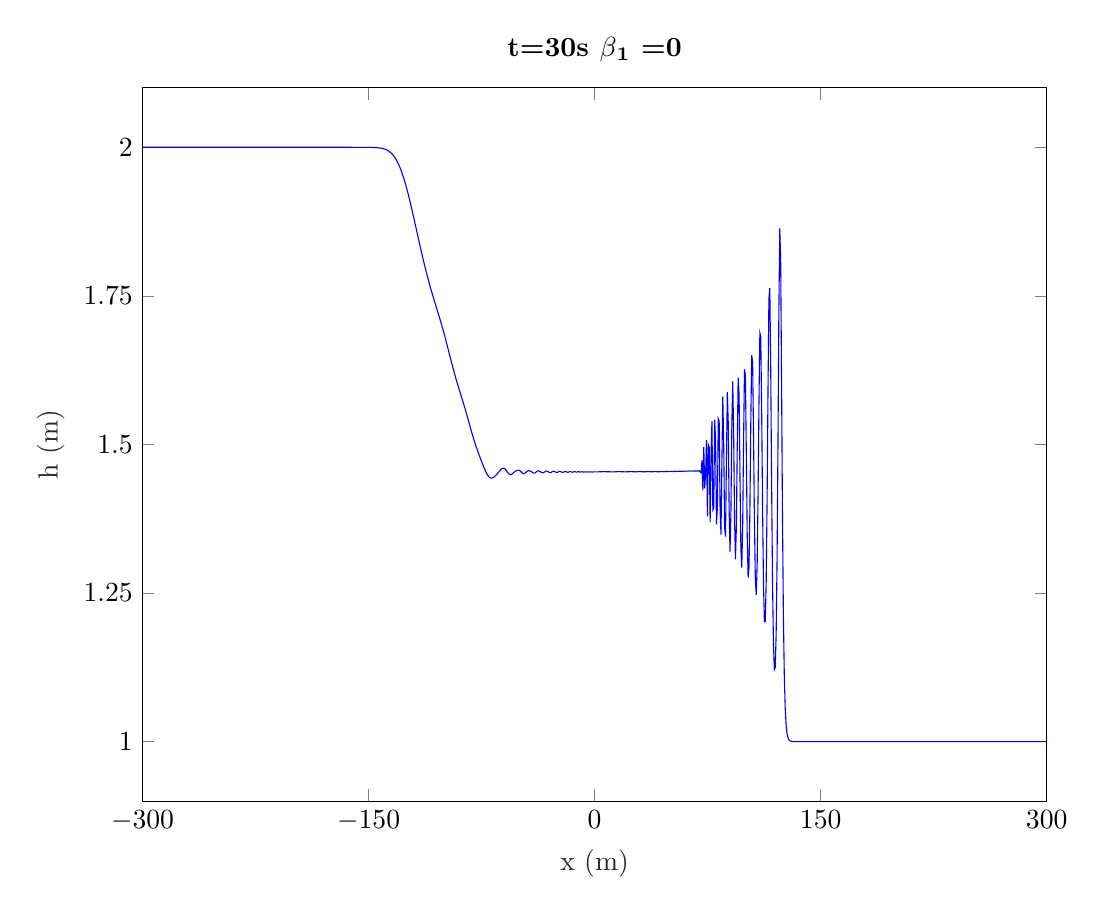
\begin{tikzpicture}

\begin{axis}[%
width=4.521in,
height=3.566in,
at={(0.758in,0.481in)},
scale only axis,
xmin=-300,
xmax=300,
xtick={-300, -150,    0,  150,  300},
xlabel style={font=\color{white!15!black}},
xlabel={x (m)},
ymin=0.9,
ymax=2.1,
ytick={   1, 1.25,  1.5, 1.75,    2},
ylabel style={font=\color{white!15!black}},
ylabel={h (m)},
axis background/.style={fill=white},
title style={font=\bfseries},
title={$\text{t=30s   }\beta{}_\text{1}\text{ =0}$}
]
\addplot [color=blue, forget plot]
  table[row sep=crcr]{%
-300.18000900045	2\\
-299.57997899895	2\\
-298.97994899745	2\\
-298.37991899595	2\\
-297.77988899445	2\\
-297.17985899295	2\\
-296.57982899145	2\\
-295.979798989949	2\\
-295.379768988449	2\\
-294.779738986949	2\\
-294.179708985449	2\\
-293.579678983949	2\\
-292.979648982449	2\\
-292.379618980949	2\\
-291.779588979449	2\\
-291.179558977949	2\\
-290.579528976449	2\\
-289.979498974949	2\\
-289.379468973449	2\\
-288.779438971949	2\\
-288.179408970449	2\\
-287.579378968948	2\\
-286.979348967448	2\\
-286.379318965948	2\\
-285.779288964448	2\\
-285.179258962948	2\\
-284.579228961448	2\\
-283.979198959948	2\\
-283.379168958448	2\\
-282.779138956948	2\\
-282.179108955448	2\\
-281.579078953948	2\\
-280.979048952448	2\\
-280.379018950948	2\\
-279.778988949447	2\\
-279.178958947947	2\\
-278.578928946447	2\\
-277.978898944947	2\\
-277.378868943447	2\\
-276.778838941947	2\\
-276.178808940447	2\\
-275.578778938947	2\\
-274.978748937447	2\\
-274.378718935947	2\\
-273.778688934447	2\\
-273.178658932947	2\\
-272.578628931447	2\\
-271.978598929946	2\\
-271.378568928446	2\\
-270.778538926946	2\\
-270.178508925446	2\\
-269.578478923946	2\\
-268.978448922446	2\\
-268.378418920946	2\\
-267.778388919446	2\\
-267.178358917946	2\\
-266.578328916446	2\\
-265.978298914946	2\\
-265.378268913446	2\\
-264.778238911946	2\\
-264.178208910446	2\\
-263.578178908945	2\\
-262.978148907445	2\\
-262.378118905945	2\\
-261.778088904445	2\\
-261.178058902945	2\\
-260.578028901445	2\\
-259.977998899945	2\\
-259.377968898445	2\\
-258.777938896945	2\\
-258.177908895445	2\\
-257.577878893945	2\\
-256.977848892445	2\\
-256.377818890945	2\\
-255.777788889444	2\\
-255.177758887944	2\\
-254.577728886444	2\\
-253.977698884944	2\\
-253.377668883444	2\\
-252.777638881944	2\\
-252.177608880444	2\\
-251.577578878944	2\\
-250.977548877444	2\\
-250.377518875944	2\\
-249.777488874444	2\\
-249.177458872944	2\\
-248.577428871444	2\\
-247.977398869943	2\\
-247.377368868443	2\\
-246.777338866943	2\\
-246.177308865443	2\\
-245.577278863943	2\\
-244.977248862443	2\\
-244.377218860943	2\\
-243.777188859443	2\\
-243.177158857943	2\\
-242.577128856443	2\\
-241.977098854943	2\\
-241.377068853443	2\\
-240.777038851943	2\\
-240.177008850443	2\\
-239.576978848942	2\\
-238.976948847442	2\\
-238.376918845942	2\\
-237.776888844442	2\\
-237.176858842942	2\\
-236.576828841442	2\\
-235.976798839942	2\\
-235.376768838442	2\\
-234.776738836942	2\\
-234.176708835442	2\\
-233.576678833942	2\\
-232.976648832442	2\\
-232.376618830942	2\\
-231.776588829441	2\\
-231.176558827941	2\\
-230.576528826441	2\\
-229.976498824941	2\\
-229.376468823441	2\\
-228.776438821941	2\\
-228.176408820441	2\\
-227.576378818941	2\\
-226.976348817441	2\\
-226.376318815941	2\\
-225.776288814441	2\\
-225.176258812941	2\\
-224.576228811441	2\\
-223.976198809941	2\\
-223.37616880844	2\\
-222.77613880694	2\\
-222.17610880544	2\\
-221.57607880394	2\\
-220.97604880244	2\\
-220.37601880094	2\\
-219.77598879944	2\\
-219.17595879794	2\\
-218.57592879644	2\\
-217.97589879494	2\\
-217.37586879344	2\\
-216.77583879194	2\\
-216.17580879044	2\\
-215.575778788939	2\\
-214.975748787439	2\\
-214.375718785939	2\\
-213.775688784439	2\\
-213.175658782939	2\\
-212.575628781439	2\\
-211.975598779939	2\\
-211.375568778439	2\\
-210.775538776939	2\\
-210.175508775439	2\\
-209.575478773939	2\\
-208.975448772439	2\\
-208.375418770939	2\\
-207.775388769438	2\\
-207.175358767938	2\\
-206.575328766438	2\\
-205.975298764938	2\\
-205.375268763438	2\\
-204.775238761938	2\\
-204.175208760438	2\\
-203.575178758938	2\\
-202.975148757438	2\\
-202.375118755938	2\\
-201.775088754438	2\\
-201.175058752938	2\\
-200.575028751438	2\\
-199.974998749937	2\\
-199.374968748437	2\\
-198.774938746937	2\\
-198.174908745437	2\\
-197.574878743937	2\\
-196.974848742437	1.99999999999999\\
-196.374818740937	1.99999999999999\\
-195.774788739437	1.99999999999997\\
-195.174758737937	1.99999999999996\\
-194.574728736437	1.99999999999994\\
-193.974698734937	1.99999999999991\\
-193.374668733437	1.99999999999987\\
-192.774638731937	1.99999999999982\\
-192.174608730437	1.99999999999975\\
-191.574578728936	1.99999999999965\\
-190.974548727436	1.99999999999951\\
-190.374518725936	1.99999999999932\\
-189.774488724436	1.99999999999906\\
-189.174458722936	1.9999999999987\\
-188.574428721436	1.99999999999821\\
-187.974398719936	1.99999999999755\\
-187.374368718436	1.99999999999664\\
-186.774338716936	1.9999999999954\\
-186.174308715436	1.99999999999371\\
-185.574278713936	1.99999999999141\\
-184.974248712436	1.99999999998829\\
-184.374218710936	1.99999999998405\\
-183.774188709435	1.99999999997829\\
-183.174158707935	1.99999999997049\\
-182.574128706435	1.99999999995994\\
-181.974098704935	1.99999999994567\\
-181.374068703435	1.9999999999264\\
-180.774038701935	1.99999999990039\\
-180.174008700435	1.99999999986534\\
-179.573978698935	1.99999999981816\\
-178.973948697435	1.99999999975473\\
-178.373918695935	1.99999999966953\\
-177.773888694435	1.99999999955523\\
-177.173858692935	1.99999999940209\\
-176.573828691435	1.99999999919715\\
-175.973798689934	1.99999999892323\\
-175.373768688434	1.99999999855755\\
-174.773738686934	1.99999999807001\\
-174.173708685434	1.9999999974208\\
-173.573678683934	1.99999999655744\\
-172.973648682434	1.99999999541079\\
-172.373618680934	1.99999999388991\\
-171.773588679434	1.99999999187538\\
-171.173558677934	1.99999998921061\\
-170.573528676434	1.99999998569057\\
-169.973498674934	1.99999998104727\\
-169.373468673434	1.999999974931\\
-168.773438671934	1.99999996688609\\
-168.173408670434	1.99999995631987\\
-167.573378668933	1.99999994246276\\
-166.973348667433	1.99999992431715\\
-166.373318665933	1.9999999005922\\
-165.773288664433	1.99999986962055\\
-165.173258662933	1.99999982925247\\
-164.573228661433	1.99999977672146\\
-163.973198659933	1.99999970847403\\
-163.373168658433	1.99999961995463\\
-162.773138656933	1.9999995053346\\
-162.173108655433	1.99999935717135\\
-161.573078653933	1.99999916598098\\
-160.973048652433	1.99999891970369\\
-160.373018650933	1.99999860303698\\
-159.772988649432	1.99999819660615\\
-159.172958647932	1.99999767593547\\
-158.572928646432	1.99999701017581\\
-157.972898644932	1.99999616053607\\
-157.372868643432	1.99999507835527\\
-156.772838641932	1.99999370274111\\
-156.172808640432	1.99999195768717\\
-155.572778638932	1.99998974856611\\
-154.972748637432	1.99998695787955\\
-154.372718635932	1.99998344012685\\
-153.772688634432	1.99997901563502\\
-153.172658632932	1.9999734631703\\
-152.572628631432	1.99996651113025\\
-151.972598629931	1.99995782709169\\
-151.372568628431	1.99994700546847\\
-150.772538626931	1.99993355301222\\
-150.172508625431	1.99991687187227\\
-149.572478623931	1.99989623991904\\
-148.972448622431	1.99987078803104\\
-148.372418620931	1.99983947405183\\
-147.772388619431	1.99980105314372\\
-147.172358617931	1.99975404430325\\
-146.572328616431	1.9996966928638\\
-145.972298614931	1.99962692889842\\
-145.372268613431	1.99954232155457\\
-144.772238611931	1.99944002950825\\
-144.172208610431	1.99931674792\\
-143.57217860893	1.99916865251421\\
-142.97214860743	1.99899134168554\\
-142.37211860593	1.99877977786202\\
-141.77208860443	1.99852822971719\\
-141.17205860293	1.99823021721658\\
-140.57202860143	1.99787846188979\\
-139.97199859993	1.99746484512191\\
-139.37196859843	1.99698037762758\\
-138.77193859693	1.99641518357818\\
-138.17190859543	1.99575850305784\\
-137.57187859393	1.99499871658757\\
-136.97184859243	1.99412339533443\\
-136.37181859093	1.99311938027632\\
-135.771788589429	1.99197289298643\\
-135.171758587929	1.99066967981626\\
-134.571728586429	1.98919519008616\\
-133.971698584929	1.98753478745812\\
-133.371668583429	1.98567399201286\\
-132.771638581929	1.98359874875598\\
-132.171608580429	1.98129571644062\\
-131.571578578929	1.97875256884168\\
-130.971548577429	1.97595829909158\\
-130.371518575929	1.97290351653463\\
-129.771488574429	1.96958072490908\\
-129.171458572929	1.96598457062993\\
-128.571428571429	1.9621120505835\\
-127.971398569929	1.9579626701679\\
-127.371368568428	1.95353854426839\\
-126.771338566928	1.94884443633207\\
-126.171308565428	1.94388773353712\\
-125.571278563928	1.93867835903409\\
-124.971248562428	1.93322862514917\\
-124.371218560928	1.92755303406533\\
-123.771188559428	1.92166803464561\\
-123.171158557928	1.91559174559081\\
-122.571128556428	1.90934365594372\\
-121.971098554928	1.90294431404519\\
-121.371068553428	1.8964150154513\\
-120.771038551928	1.88977749913296\\
-120.171008550428	1.88305365962891\\
-119.570978548927	1.87626528086855\\
-118.970948547427	1.86943379528152\\
-118.370918545927	1.86258006972059\\
-117.770888544427	1.85572421777455\\
-117.170858542927	1.8488854363456\\
-116.570828541427	1.84208186298789\\
-115.970798539927	1.83533044950076\\
-115.370768538427	1.82864684666935\\
-114.770738536927	1.82204529485661\\
-114.170708535427	1.81553851537619\\
-113.570678533927	1.80913759820972\\
-112.970648532427	1.80285188267146\\
-112.370618530927	1.79668882906245\\
-111.770588529426	1.79065388118893\\
-111.170558527926	1.78475032183093\\
-110.570528526426	1.77897912580118\\
-109.970498524926	1.77333881806762\\
-109.370468523426	1.76782534740837\\
-108.770438521926	1.76243198905043\\
-108.170408520426	1.7571492924566\\
-107.570378518926	1.7519650925351\\
-106.970348517426	1.74686460364336\\
-106.370318515926	1.74183061538509\\
-105.770288514426	1.73684380690414\\
-105.170258512926	1.73188319177837\\
-104.570228511426	1.72692669849767\\
-103.970198509925	1.72195188192517\\
-103.370168508425	1.71693674949798\\
-102.770138506925	1.71186067304164\\
-102.170108505425	1.70670534417009\\
-101.570078503925	1.70145571984574\\
-100.970048502425	1.69610089642978\\
-100.370018500925	1.69063484697892\\
-99.769988499425	1.6850569587332\\
-99.1699584979249	1.67937231610938\\
-98.5699284964248	1.67359168864778\\
-97.9698984949247	1.66773120200644\\
-97.3698684934247	1.66181169134845\\
-96.7698384919246	1.65585775809404\\
-96.1698084904245	1.64989657086929\\
-95.5697784889244	1.64395646793464\\
-94.9697484874244	1.63806543055556\\
-94.3697184859243	1.63224950469774\\
-93.7696884844242	1.62653125284218\\
-93.1696584829241	1.62092831977388\\
-92.5696284814241	1.61545219697676\\
-91.969598479924	1.61010727025151\\
-91.3695684784239	1.60489023383217\\
-90.7695384769239	1.59978994984758\\
-90.1695084754238	1.59478782157374\\
-89.5694784739237	1.5898587290593\\
-88.9694484724236	1.58497254321501\\
-88.3694184709235	1.58009618775065\\
-87.7693884694235	1.5751961587378\\
-87.1693584679234	1.57024134428918\\
-86.5693284664233	1.56520592117721\\
-85.9692984649232	1.56007205352378\\
-85.3692684634232	1.55483209406155\\
-84.7692384619231	1.5494900014441\\
-84.169208460423	1.54406174240308\\
-83.5691784589229	1.53857454200925\\
-82.9691484574229	1.53306496772158\\
-82.3691184559228	1.52757596656684\\
-81.7690884544227	1.52215310146679\\
-81.1690584529227	1.51684033705379\\
-80.5690284514226	1.51167579760153\\
-79.9689984499225	1.50668795614029\\
-79.3689684484224	1.50189271404358\\
-78.7689384469223	1.49729179352756\\
-78.1689084454223	1.49287278712354\\
-77.5688784439222	1.48861107991051\\
-76.9688484424221	1.48447367397554\\
-76.368818440922	1.48042470030017\\
-75.768788439422	1.47643211873351\\
-75.1687584379219	1.47247482308068\\
-74.5687284364218	1.46854914761802\\
-73.9686984349217	1.46467368249405\\
-73.3686684334217	1.4608914018526\\
-72.7686384319216	1.45726840539472\\
-72.1686084304215	1.45388903751186\\
-71.5685784289215	1.45084770263463\\
-70.9685484274214	1.44823824842141\\
-70.3685184259213	1.44614225785157\\
-69.7684884244212	1.44461792011593\\
-69.1684584229211	1.4436912971977\\
-68.5684284214211	1.44335159708397\\
-67.968398419921	1.44355262405937\\
-67.3683684184209	1.44421838012284\\
-66.7683384169208	1.44525633478781\\
-66.1683084154208	1.44657175602335\\
-65.5682784139207	1.44808189867486\\
-64.9682484124206	1.44972460554737\\
-64.3682184109205	1.45145752363213\\
-63.7681884094205	1.45324638713938\\
-63.1681584079204	1.4550447326789\\
-62.5681284064203	1.45677179610667\\
-61.9680984049203	1.45829856414819\\
-61.3680684034202	1.45945213089634\\
-60.7680384019201	1.46004426820002\\
-60.16800840042	1.45992150518959\\
-59.5679783989199	1.4590235206149\\
-58.9679483974199	1.45742861694046\\
-58.3679183959198	1.45536512747742\\
-57.7678883944197	1.45317705192673\\
-57.1678583929196	1.45124882318097\\
-56.5678283914196	1.44991049525733\\
-55.9677983899195	1.44935400751013\\
-55.3677683884194	1.44958944669234\\
-54.7677383869193	1.45045837107734\\
-54.1677083854193	1.45170007164572\\
-53.5676783839192	1.4530450884317\\
-52.9676483824191	1.45429445326696\\
-52.3676183809191	1.45534693010761\\
-51.767588379419	1.45616288258479\\
-51.1675583779189	1.45669284257225\\
-50.5675283764188	1.4568278759005\\
-49.9674983749187	1.45642386741632\\
-49.3674683734187	1.45540608183479\\
-48.7674383719186	1.45389628588807\\
-48.1674083704185	1.45226539679638\\
-47.5673783689184	1.4510400518793\\
-46.9673483674184	1.45067873784103\\
-46.3673183659183	1.45132907339051\\
-45.7672883644182	1.45272115863986\\
-45.1672583629181	1.45428486219313\\
-44.5672283614181	1.45544801764324\\
-43.967198359918	1.45592463284614\\
-43.3671683584179	1.45578845228767\\
-42.7671383569178	1.45528761535977\\
-42.1671083554178	1.45458657785403\\
-41.5670783539177	1.4536988697903\\
-40.9670483524176	1.45268465780774\\
-40.3670183509175	1.45187666879645\\
-39.7669883494175	1.45179613373611\\
-39.1669583479174	1.45271016701157\\
-38.5669283464173	1.45423341414019\\
-37.9668983449172	1.45547827781706\\
-37.3668683434172	1.45575386313983\\
-36.7668383419171	1.45513367373592\\
-36.166808340417	1.4542337927927\\
-35.5667783389169	1.45347869018736\\
-34.9667483374168	1.45284494241188\\
-34.3667183359168	1.45240149807475\\
-33.7666883344167	1.45264961225137\\
-33.1666583329167	1.45381557830059\\
-32.5666283314166	1.45508927374733\\
-31.9665983299165	1.45537850033799\\
-31.3665683284164	1.45472806191536\\
-30.7665383269164	1.45397216645986\\
-30.1665083254163	1.45328217601901\\
-29.5664783239162	1.45261884722491\\
-28.9664483224161	1.45281339387857\\
-28.3664183209161	1.45398492526912\\
-27.766388319416	1.4547631930896\\
-27.1663583179159	1.45487249514906\\
-26.5663283164158	1.45459888585591\\
-25.9662983149157	1.4535253052561\\
-25.3662683134157	1.45292204671782\\
-24.7662383119156	1.45304016026925\\
-24.1662083104155	1.4537808247432\\
-23.5661783089154	1.45459328613229\\
-22.9661483074154	1.45478034560382\\
-22.3661183059153	1.45416983563743\\
-21.7660883044152	1.45333870987349\\
-21.1660583029151	1.45304091344464\\
-20.5660283014151	1.4535548472357\\
-19.965998299915	1.45436070910111\\
-19.3659682984149	1.45463658740194\\
-18.7659382969148	1.45409007079115\\
-18.1659082954148	1.45334060374096\\
-17.5658782939147	1.4532309379765\\
-16.9658482924146	1.45388643533311\\
-16.3658182909145	1.45448962516212\\
-15.7657882894144	1.45426689958611\\
-15.1657582879144	1.45353398014688\\
-14.5657282864143	1.45330182544774\\
-13.9656982849143	1.45388339470283\\
-13.3656682834142	1.45439720539181\\
-12.7656382819141	1.45404214366442\\
-12.165608280414	1.45340636404645\\
-11.565578278914	1.45356346319781\\
-10.9655482774139	1.45420666811049\\
-10.3655182759138	1.45412521319022\\
-9.76548827441371	1.45349109005637\\
-9.16545827291367	1.45359239623411\\
-8.56542827141357	1.45416224906575\\
-7.96539826991352	1.45388889965508\\
-7.36536826841342	1.45343151903948\\
-6.76533826691332	1.45388907147954\\
-6.16530826541327	1.45398932665468\\
-5.56527826391317	1.45347705307128\\
-4.96524826241313	1.4538546531467\\
-4.36521826091303	1.45388419224482\\
-3.76518825941298	1.45352640039674\\
-3.16515825791288	1.45394931158433\\
-2.56512825641283	1.45359387028309\\
-1.96509825491273	1.4538635014082\\
-1.36506825341269	1.45368190934\\
-0.765038251912586	1.4538291330321\\
-0.165008250412541	1.45378397435933\\
0.435021751087561	1.45382586979734\\
1.03505175258761	1.45387219944204\\
1.63508175408771	1.45392011724347\\
2.23511175558775	1.4539694141278\\
2.83514175708785	1.45401676063771\\
3.43517175858796	1.45406242110314\\
4.035201760088	1.45410915767045\\
4.6352317615881	1.45415756432989\\
5.23526176308815	1.45419399643015\\
5.83529176458825	1.45422332181229\\
6.43532176608829	1.45422477112504\\
7.03535176758839	1.45421583220929\\
7.63538176908844	1.4541873262193\\
8.23541177058854	1.45414960924303\\
8.83544177208859	1.45411405796006\\
9.43547177358869	1.45406874720269\\
10.0355017750887	1.45402447637352\\
10.6355317765888	1.4539900217264\\
11.2355617780889	1.45395970671641\\
11.835591779589	1.45394258794773\\
12.435621781089	1.45395376791978\\
13.0356517825891	1.45398990377292\\
13.6356817840892	1.45403966596928\\
14.2357117855893	1.45409886219182\\
14.8357417870894	1.45416205054849\\
15.4357717885894	1.45421353477905\\
16.0358017900895	1.45423768908232\\
16.6358317915896	1.45423203258008\\
17.2358617930897	1.45420401217967\\
17.8358917945897	1.45416066014051\\
18.4359217960898	1.4541065914772\\
19.0359517975899	1.45405032784935\\
19.63598179909	1.45400669159981\\
20.23601180059	1.45399001603506\\
20.8360418020901	1.45400554042679\\
21.4360718035902	1.45404744380132\\
22.0361018050903	1.45410365848422\\
22.6361318065904	1.45416101003969\\
23.2361618080904	1.45420704296776\\
23.8361918095905	1.45423017615428\\
24.4362218110905	1.45422174471421\\
25.0362518125906	1.45418060397568\\
25.6362818140907	1.45411708041284\\
26.2363118155908	1.45405220284409\\
26.8363418170908	1.45401073470438\\
27.4363718185909	1.45401065399043\\
28.036401820091	1.4540543910493\\
28.6364318215911	1.45412637772679\\
29.2364618230911	1.45419838080502\\
29.8364918245912	1.45424050812401\\
30.4365218260913	1.4542337008448\\
31.0365518275914	1.45417883998099\\
31.6365818290914	1.45409814484725\\
32.2366118305915	1.45402730180063\\
32.8366418320916	1.45400048297784\\
33.4366718335917	1.45403390304788\\
34.0367018350918	1.45411587310108\\
34.6367318365918	1.45420903920826\\
35.2367618380919	1.45426691100796\\
35.836791839592	1.45425785068083\\
36.4368218410921	1.45418463148923\\
37.0368518425921	1.45408714163735\\
37.6368818440922	1.45402296159785\\
38.2369118455923	1.4540336741857\\
38.8369418470924	1.45411624504621\\
39.4369718485924	1.45421979534732\\
40.0370018500925	1.45427491103737\\
40.6370318515926	1.45424106817563\\
41.2370618530927	1.45414098453801\\
41.8370918545928	1.45405225755919\\
42.4371218560928	1.45405404191305\\
43.0371518575929	1.45416299025487\\
43.6371818590929	1.45431078797196\\
44.237211860593	1.45439138963917\\
44.8372418620931	1.4543502566683\\
45.4372718635932	1.45424142609526\\
46.0373018650932	1.45418972545567\\
46.6373318665933	1.45427552091842\\
47.2373618680934	1.45444513127826\\
47.8373918695935	1.45454861475307\\
48.4374218710935	1.45449363475031\\
49.0374518725936	1.45436216488673\\
49.6374818740937	1.45433915850599\\
50.2375118755938	1.45449758309171\\
50.8375418770938	1.45468538092156\\
51.4375718785939	1.45469390251014\\
52.037601880094	1.45454216390084\\
52.6376318815941	1.45448724889123\\
53.2376618830942	1.45467126039601\\
53.8376918845942	1.45487395130688\\
54.4377218860943	1.45481591875243\\
55.0377518875944	1.45463703922393\\
55.6377818890945	1.45471838926134\\
56.2378118905945	1.45499703094956\\
56.8378418920946	1.45500817117962\\
57.4378718935947	1.45479013117225\\
58.0379018950948	1.45489585412572\\
58.6379318965948	1.45519784606221\\
59.2379618980949	1.45506912931337\\
59.837991899595	1.45491805946838\\
60.4380219010951	1.45525754726532\\
61.0380519025952	1.45522485695741\\
61.6380819040952	1.45498928397457\\
62.2381119055953	1.4553780307169\\
62.8381419070953	1.45516038305567\\
63.4381719085955	1.4551940199594\\
64.0382019100955	1.45533718574536\\
64.6382319115956	1.45519099708883\\
65.2382619130956	1.45528947885056\\
65.8382919145957	1.45532017135983\\
66.4383219160958	1.45530685851074\\
67.0383519175959	1.45533558384612\\
67.6383819190959	1.45538028448584\\
68.238411920596	1.45540123025942\\
68.8384419220961	1.45537772167214\\
69.4384719235962	1.45607525213326\\
70.0385019250962	1.45367825983783\\
70.6385319265963	1.45253625148847\\
71.2385619280964	1.4729841353567\\
71.8385919295965	1.42260884626533\\
72.4386219310966	1.49533536862749\\
73.0386519325966	1.42633728668756\\
73.6386819340967	1.45002433182862\\
74.2387119355968	1.50777843264391\\
74.8387419370969	1.37889389012167\\
75.4387719385969	1.49939860063668\\
76.038801940097	1.49538528420114\\
76.6388319415971	1.36897876698112\\
77.2388619430972	1.48031322742535\\
77.8388919445972	1.53916222409342\\
78.4389219460973	1.38957716436667\\
79.0389519475974	1.39285166117688\\
79.6389819490975	1.54182901612949\\
80.2390119505975	1.50841599381552\\
80.8390419520976	1.36549423752042\\
81.4390719535977	1.39354068393491\\
82.0391019550977	1.54313764081951\\
82.6391319565979	1.53914931954709\\
83.2391619580979	1.39043298168387\\
83.839191959598	1.34846238735052\\
84.439221961098	1.47143155157524\\
85.0392519625981	1.58054110854061\\
85.6392819640982	1.50052811025023\\
86.2393119655983	1.36029055925645\\
86.8393419670983	1.34498254141285\\
87.4393719685984	1.46996892444967\\
88.0394019700985	1.58791439240573\\
88.6394319715986	1.5377702957113\\
89.2394619730986	1.39129693759819\\
89.8394919745987	1.31971844647142\\
90.4395219760988	1.38568873206115\\
91.0395519775989	1.53201694246294\\
91.639581979099	1.60599621077866\\
92.239611980599	1.51869094815614\\
92.8396419820991	1.3743697324043\\
93.4396719835992	1.30684642640933\\
94.0397019850993	1.36002614484794\\
94.6397319865993	1.4994451852671\\
95.2397619880994	1.61263557117597\\
95.8397919895995	1.58527781643922\\
96.4398219910996	1.44780721314315\\
97.0398519925996	1.32466542467927\\
97.6398819940997	1.29269352542484\\
98.2399119955998	1.36531205586165\\
98.8399419970999	1.50826050872623\\
99.4399719985999	1.62646952778163\\
100.0400020001	1.61653153752288\\
100.6400320016	1.48912241752283\\
101.2400620031	1.3495441101087\\
101.8400920046	1.27620678558769\\
102.4401220061	1.29267771183622\\
103.0401520076	1.39338466084146\\
103.6401820091	1.54089365351249\\
104.240212010601	1.65020963459095\\
104.840242012101	1.63793854184896\\
105.440272013601	1.51540564421351\\
106.040302015101	1.37050987232412\\
106.640332016601	1.27285926836662\\
107.240362018101	1.24679808223841\\
107.840392019601	1.29586846033571\\
108.440422021101	1.41456823087406\\
109.040452022601	1.57118572656393\\
109.640482024101	1.68769052605303\\
110.240512025601	1.6814818940583\\
110.840542027101	1.55541589151048\\
111.440572028601	1.39281140912491\\
112.040602030102	1.26625882993818\\
112.640632031602	1.20172594479208\\
113.240662033102	1.20189019267835\\
113.840692034602	1.26908683926881\\
114.440722036102	1.40601298396003\\
115.040752037602	1.59098535976334\\
115.640782039102	1.74502378454096\\
116.240812040602	1.76311432529741\\
116.840842042102	1.62818236207839\\
117.440872043602	1.43309662397987\\
118.040902045102	1.26902723280051\\
118.640932046602	1.16659482416312\\
119.240962048102	1.12111740723372\\
119.840992049603	1.12479950564048\\
120.441022051103	1.18032284250784\\
121.041052052603	1.30095332733118\\
121.641082054103	1.49442715587025\\
122.241112055603	1.72117193072469\\
122.841142057103	1.86337880386055\\
123.441172058603	1.81195644365813\\
124.041202060103	1.60696096708632\\
124.641232061603	1.38114196735124\\
125.241262063103	1.21414964650954\\
125.841292064603	1.11295594114526\\
126.441322066103	1.05761827701741\\
127.041352067603	1.02889452703206\\
127.641382069103	1.01436853049113\\
128.241412070604	1.00711622511135\\
128.841442072104	1.00351786389442\\
129.441472073604	1.00173769698008\\
130.041502075104	1.00085816324925\\
130.641532076604	1.00042382186095\\
131.241562078104	1.00020934965431\\
131.841592079604	1.00010343442905\\
132.441622081104	1.00005111821875\\
133.041652082604	1.0000252702846\\
133.641682084104	1.00001249598183\\
134.241712085604	1.00000618096189\\
134.841742087104	1.00000305819513\\
135.441772088604	1.00000151354238\\
136.041802090105	1.00000074927293\\
136.641832091605	1.00000037101922\\
137.241862093105	1.00000018376281\\
137.841892094605	1.00000009103673\\
138.441922096105	1.00000004510925\\
139.041952097605	1.00000002235608\\
139.641982099105	1.00000001108146\\
140.242012100605	1.00000000549363\\
140.842042102105	1.00000000272377\\
141.442072103605	1.00000000135057\\
142.042102105105	1.00000000066971\\
142.642132106605	1.0000000003321\\
143.242162108105	1.00000000016468\\
143.842192109605	1.00000000008166\\
144.442222111106	1.00000000004048\\
145.042252112606	1.00000000002007\\
145.642282114106	1.00000000000994\\
146.242312115606	1.00000000000492\\
146.842342117106	1.00000000000244\\
147.442372118606	1.0000000000012\\
148.042402120106	1.00000000000059\\
148.642432121606	1.00000000000029\\
149.242462123106	1.00000000000014\\
149.842492124606	1.00000000000006\\
150.442522126106	1.00000000000003\\
151.042552127606	1.00000000000001\\
151.642582129106	1\\
152.242612130607	1\\
152.842642132107	1\\
153.442672133607	1\\
154.042702135107	1\\
154.642732136607	1\\
155.242762138107	1\\
155.842792139607	1\\
156.442822141107	1\\
157.042852142607	1\\
157.642882144107	1\\
158.242912145607	1\\
158.842942147107	1\\
159.442972148607	1\\
160.043002150107	1\\
160.643032151608	1\\
161.243062153108	1\\
161.843092154608	1\\
162.443122156108	1\\
163.043152157608	1\\
163.643182159108	1\\
164.243212160608	1\\
164.843242162108	1\\
165.443272163608	1\\
166.043302165108	1\\
166.643332166608	1\\
167.243362168108	1\\
167.843392169608	1\\
168.443422171109	1\\
169.043452172609	1\\
169.643482174109	1\\
170.243512175609	1\\
170.843542177109	1\\
171.443572178609	1\\
172.043602180109	1\\
172.643632181609	1\\
173.243662183109	1\\
173.843692184609	1\\
174.443722186109	1\\
175.043752187609	1\\
175.643782189109	1\\
176.24381219061	1\\
176.84384219211	1\\
177.44387219361	1\\
178.04390219511	1\\
178.64393219661	1\\
179.24396219811	1\\
179.84399219961	1\\
180.44402220111	1\\
181.04405220261	1\\
181.64408220411	1\\
182.24411220561	1\\
182.84414220711	1\\
183.44417220861	1\\
184.04420221011	1\\
184.644232211611	1\\
185.244262213111	1\\
185.844292214611	1\\
186.444322216111	1\\
187.044352217611	1\\
187.644382219111	1\\
188.244412220611	1\\
188.844442222111	1\\
189.444472223611	1\\
190.044502225111	1\\
190.644532226611	1\\
191.244562228111	1\\
191.844592229611	1\\
192.444622231112	1\\
193.044652232612	1\\
193.644682234112	1\\
194.244712235612	1\\
194.844742237112	1\\
195.444772238612	1\\
196.044802240112	1\\
196.644832241612	1\\
197.244862243112	1\\
197.844892244612	1\\
198.444922246112	1\\
199.044952247612	1\\
199.644982249112	1\\
200.245012250613	1\\
200.845042252113	1\\
201.445072253613	1\\
202.045102255113	1\\
202.645132256613	1\\
203.245162258113	1\\
203.845192259613	1\\
204.445222261113	1\\
205.045252262613	1\\
205.645282264113	1\\
206.245312265613	1\\
206.845342267113	1\\
207.445372268613	1\\
208.045402270114	1\\
208.645432271614	1\\
209.245462273114	1\\
209.845492274614	1\\
210.445522276114	1\\
211.045552277614	1\\
211.645582279114	1\\
212.245612280614	1\\
212.845642282114	1\\
213.445672283614	1\\
214.045702285114	1\\
214.645732286614	1\\
215.245762288114	1\\
215.845792289614	1\\
216.445822291115	1\\
217.045852292615	1\\
217.645882294115	1\\
218.245912295615	1\\
218.845942297115	1\\
219.445972298615	1\\
220.046002300115	1\\
220.646032301615	1\\
221.246062303115	1\\
221.846092304615	1\\
222.446122306115	1\\
223.046152307615	1\\
223.646182309115	1\\
224.246212310616	1\\
224.846242312116	1\\
225.446272313616	1\\
226.046302315116	1\\
226.646332316616	1\\
227.246362318116	1\\
227.846392319616	1\\
228.446422321116	1\\
229.046452322616	1\\
229.646482324116	1\\
230.246512325616	1\\
230.846542327116	1\\
231.446572328616	1\\
232.046602330116	1\\
232.646632331617	1\\
233.246662333117	1\\
233.846692334617	1\\
234.446722336117	1\\
235.046752337617	1\\
235.646782339117	1\\
236.246812340617	1\\
236.846842342117	1\\
237.446872343617	1\\
238.046902345117	1\\
238.646932346617	1\\
239.246962348117	1\\
239.846992349617	1\\
240.447022351118	1\\
241.047052352618	1\\
241.647082354118	1\\
242.247112355618	1\\
242.847142357118	1\\
243.447172358618	1\\
244.047202360118	1\\
244.647232361618	1\\
245.247262363118	1\\
245.847292364618	1\\
246.447322366118	1\\
247.047352367618	1\\
247.647382369118	1\\
248.247412370619	1\\
248.847442372119	1\\
249.447472373619	1\\
250.047502375119	1\\
250.647532376619	1\\
251.247562378119	1\\
251.847592379619	1\\
252.447622381119	1\\
253.047652382619	1\\
253.647682384119	1\\
254.247712385619	1\\
254.847742387119	1\\
255.447772388619	1\\
256.04780239012	1\\
256.64783239162	1\\
257.24786239312	1\\
257.84789239462	1\\
258.44792239612	1\\
259.04795239762	1\\
259.64798239912	1\\
260.24801240062	1\\
260.84804240212	1\\
261.44807240362	1\\
262.04810240512	1\\
262.64813240662	1\\
263.24816240812	1\\
263.84819240962	1\\
264.448222411121	1\\
265.048252412621	1\\
265.648282414121	1\\
266.248312415621	1\\
266.848342417121	1\\
267.448372418621	1\\
268.048402420121	1\\
268.648432421621	1\\
269.248462423121	1\\
269.848492424621	1\\
270.448522426121	1\\
271.048552427621	1\\
271.648582429121	1\\
272.248612430622	1\\
272.848642432122	1\\
273.448672433622	1\\
274.048702435122	1\\
274.648732436622	1\\
275.248762438122	1\\
275.848792439622	1\\
276.448822441122	1\\
277.048852442622	1\\
277.648882444122	1\\
278.248912445622	1\\
278.848942447122	1\\
279.448972448622	1\\
280.049002450123	1\\
280.649032451623	1\\
281.249062453123	1\\
281.849092454623	1\\
282.449122456123	1\\
283.049152457623	1\\
283.649182459123	1\\
284.249212460623	1\\
284.849242462123	1\\
285.449272463623	1\\
286.049302465123	1\\
286.649332466623	1\\
287.249362468123	1\\
287.849392469623	1\\
288.449422471124	1\\
289.049452472624	1\\
289.649482474124	1\\
290.249512475624	1\\
290.849542477124	1\\
291.449572478624	1\\
292.049602480124	1\\
292.649632481624	1\\
293.249662483124	1\\
293.849692484624	1\\
294.449722486124	1\\
295.049752487624	1\\
295.649782489125	1\\
296.249812490625	1\\
296.849842492125	1\\
297.449872493625	1\\
298.049902495125	1\\
298.649932496625	1\\
299.249962498125	1\\
299.849992499625	1\\
};
\end{axis}
\end{tikzpicture}%
	\caption{$t=30s$}
	\end{subfigure}
	\begin{subfigure}{0.49\textwidth}
	\centering
	% This file was created by matlab2tikz.
%
%The latest updates can be retrieved from
%  http://www.mathworks.com/matlabcentral/fileexchange/22022-matlab2tikz-matlab2tikz
%where you can also make suggestions and rate matlab2tikz.
%
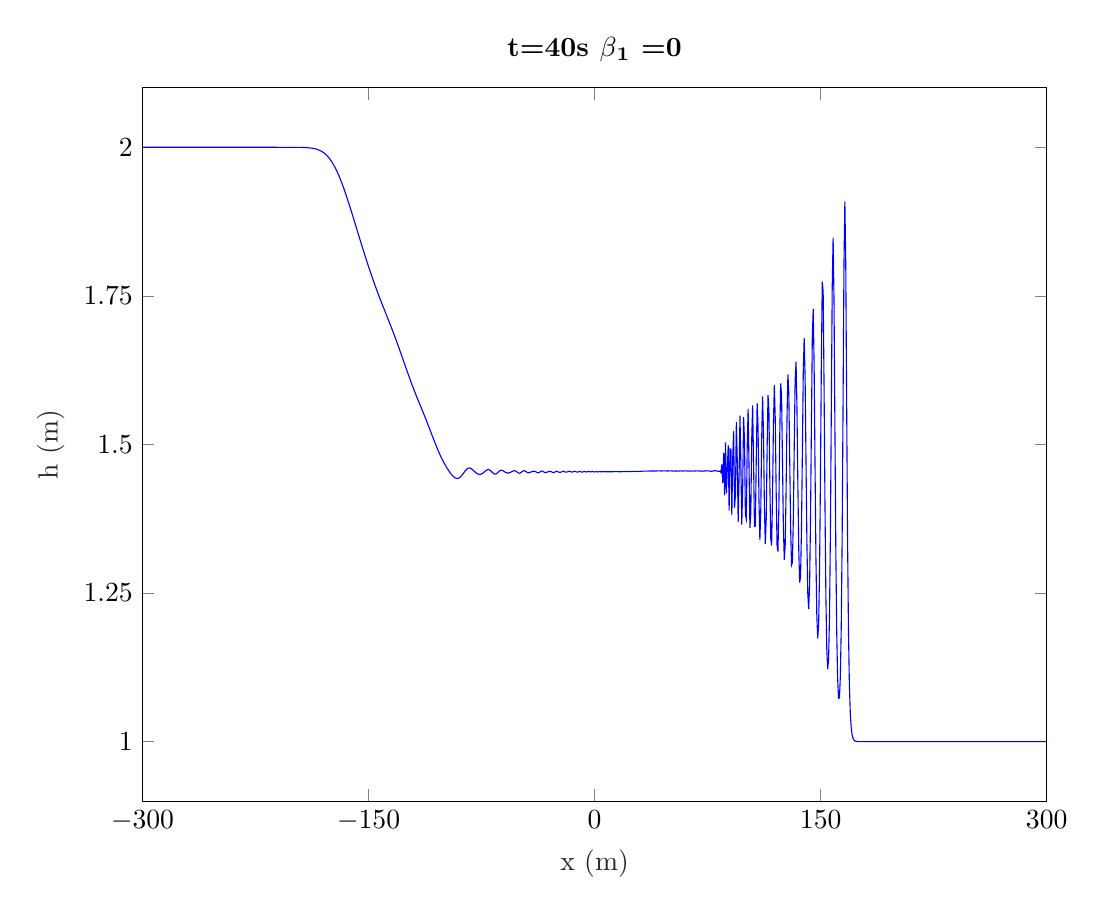
\begin{tikzpicture}

\begin{axis}[%
width=4.521in,
height=3.566in,
at={(0.758in,0.481in)},
scale only axis,
xmin=-300,
xmax=300,
xtick={-300, -150,    0,  150,  300},
xlabel style={font=\color{white!15!black}},
xlabel={x (m)},
ymin=0.9,
ymax=2.1,
ytick={   1, 1.25,  1.5, 1.75,    2},
ylabel style={font=\color{white!15!black}},
ylabel={h (m)},
axis background/.style={fill=white},
title style={font=\bfseries},
title={$\text{t=40s   }\beta{}_\text{1}\text{ =0}$}
]
\addplot [color=blue, forget plot]
  table[row sep=crcr]{%
-300.18000900045	2\\
-299.57997899895	2\\
-298.97994899745	2\\
-298.37991899595	2\\
-297.77988899445	2\\
-297.17985899295	2\\
-296.57982899145	2\\
-295.979798989949	2\\
-295.379768988449	2\\
-294.779738986949	2\\
-294.179708985449	2\\
-293.579678983949	2\\
-292.979648982449	2\\
-292.379618980949	2\\
-291.779588979449	2\\
-291.179558977949	2\\
-290.579528976449	2\\
-289.979498974949	2\\
-289.379468973449	2\\
-288.779438971949	2\\
-288.179408970449	2\\
-287.579378968948	2\\
-286.979348967448	2\\
-286.379318965948	2\\
-285.779288964448	2\\
-285.179258962948	2\\
-284.579228961448	2\\
-283.979198959948	2\\
-283.379168958448	2\\
-282.779138956948	2\\
-282.179108955448	2\\
-281.579078953948	2\\
-280.979048952448	2\\
-280.379018950948	2\\
-279.778988949447	2\\
-279.178958947947	2\\
-278.578928946447	2\\
-277.978898944947	2\\
-277.378868943447	2\\
-276.778838941947	2\\
-276.178808940447	2\\
-275.578778938947	2\\
-274.978748937447	2\\
-274.378718935947	2\\
-273.778688934447	2\\
-273.178658932947	2\\
-272.578628931447	2\\
-271.978598929946	2\\
-271.378568928446	2\\
-270.778538926946	2\\
-270.178508925446	2\\
-269.578478923946	2\\
-268.978448922446	2\\
-268.378418920946	2\\
-267.778388919446	2\\
-267.178358917946	2\\
-266.578328916446	2\\
-265.978298914946	2\\
-265.378268913446	2\\
-264.778238911946	2\\
-264.178208910446	2\\
-263.578178908945	2\\
-262.978148907445	2\\
-262.378118905945	2\\
-261.778088904445	2\\
-261.178058902945	2\\
-260.578028901445	2\\
-259.977998899945	2\\
-259.377968898445	2\\
-258.777938896945	2\\
-258.177908895445	2\\
-257.577878893945	2\\
-256.977848892445	2\\
-256.377818890945	2\\
-255.777788889444	2\\
-255.177758887944	2\\
-254.577728886444	2\\
-253.977698884944	2\\
-253.377668883444	2\\
-252.777638881944	2\\
-252.177608880444	2\\
-251.577578878944	2\\
-250.977548877444	1.99999999999999\\
-250.377518875944	1.99999999999999\\
-249.777488874444	1.99999999999998\\
-249.177458872944	1.99999999999996\\
-248.577428871444	1.99999999999995\\
-247.977398869943	1.99999999999992\\
-247.377368868443	1.99999999999989\\
-246.777338866943	1.99999999999985\\
-246.177308865443	1.99999999999979\\
-245.577278863943	1.99999999999972\\
-244.977248862443	1.99999999999962\\
-244.377218860943	1.99999999999949\\
-243.777188859443	1.99999999999932\\
-243.177158857943	1.99999999999909\\
-242.577128856443	1.99999999999879\\
-241.977098854943	1.9999999999984\\
-241.377068853443	1.99999999999788\\
-240.777038851943	1.9999999999972\\
-240.177008850443	1.9999999999963\\
-239.576978848942	1.99999999999512\\
-238.976948847442	1.99999999999357\\
-238.376918845942	1.99999999999155\\
-237.776888844442	1.99999999998889\\
-237.176858842942	1.99999999998542\\
-236.576828841442	1.99999999998088\\
-235.976798839942	1.99999999997496\\
-235.376768838442	1.99999999996722\\
-234.776738836942	1.99999999995714\\
-234.176708835442	1.999999999944\\
-233.576678833942	1.99999999992692\\
-232.976648832442	1.9999999999047\\
-232.376618830942	1.99999999987584\\
-231.776588829441	1.9999999998384\\
-231.176558827941	1.99999999978987\\
-230.576528826441	1.99999999972701\\
-229.976498824941	1.99999999964569\\
-229.376468823441	1.99999999954057\\
-228.776438821941	1.99999999940485\\
-228.176408820441	1.99999999922978\\
-227.576378818941	1.9999999990042\\
-226.976348817441	1.99999999871382\\
-226.376318815941	1.99999999834042\\
-225.776288814441	1.99999999786077\\
-225.176258812941	1.9999999972453\\
-224.576228811441	1.99999999645639\\
-223.976198809941	1.9999999954463\\
-223.37616880844	1.9999999941544\\
-222.77613880694	1.99999999250393\\
-222.17610880544	1.99999999039773\\
-221.57607880394	1.99999998771303\\
-220.97604880244	1.99999998429486\\
-220.37601880094	1.9999999799479\\
-219.77598879944	1.99999997442628\\
-219.17595879794	1.99999996742091\\
-218.57592879644	1.99999995854377\\
-217.97589879494	1.99999994730845\\
-217.37586879344	1.99999993310598\\
-216.77583879194	1.99999991517515\\
-216.17580879044	1.99999989256574\\
-215.575778788939	1.99999986409337\\
-214.975748787439	1.99999982828398\\
-214.375718785939	1.99999978330579\\
-213.775688784439	1.99999972688595\\
-213.175658782939	1.99999965620878\\
-212.575628781439	1.99999956779162\\
-211.975598779939	1.99999945733384\\
-211.375568778439	1.99999931953338\\
-210.775538776939	1.99999914786449\\
-210.175508775439	1.99999893430894\\
-209.575478773939	1.99999866903169\\
-208.975448772439	1.99999833999042\\
-208.375418770939	1.99999793246651\\
-207.775388769438	1.99999742850312\\
-207.175358767938	1.99999680623337\\
-206.575328766438	1.99999603907946\\
-205.975298764938	1.9999950948\\
-205.375268763438	1.9999939343604\\
-204.775238761938	1.9999925105964\\
-204.175208760438	1.99999076663814\\
-203.575178758938	1.99998863405672\\
-202.975148757438	1.99998603069146\\
-202.375118755938	1.99998285811078\\
-201.775088754438	1.99997899865478\\
-201.175058752938	1.99997431200243\\
-200.575028751438	1.99996863120137\\
-199.974998749937	1.99996175809343\\
-199.374968748437	1.99995345806459\\
-198.774938746937	1.99994345404482\\
-198.174908745437	1.99993141968037\\
-197.574878743937	1.99991697160025\\
-196.974848742437	1.99989966069977\\
-196.374818740937	1.99987896236713\\
-195.774788739437	1.99985426558591\\
-195.174758737937	1.99982486085668\\
-194.574728736437	1.99978992689566\\
-193.974698734937	1.99974851608886\\
-193.374668733437	1.99969953870608\\
-192.774638731937	1.99964174591217\\
-192.174608730437	1.99957371165338\\
-191.574578728936	1.99949381354472\\
-190.974548727436	1.99940021294067\\
-190.374518725936	1.99929083443587\\
-189.774488724436	1.99916334511475\\
-189.174458722936	1.99901513394763\\
-188.574428721436	1.99884329181502\\
-187.974398719936	1.99864459272876\\
-187.374368718436	1.99841547690547\\
-186.774338716936	1.99815203643126\\
-186.174308715436	1.99785000433042\\
-185.574278713936	1.9975047479124\\
-184.974248712436	1.99711126731097\\
-184.374218710936	1.99666420014449\\
-183.774188709435	1.99615783320612\\
-183.174158707935	1.99558612203525\\
-182.574128706435	1.99494271911704\\
-181.974098704935	1.99422101130498\\
-181.374068703435	1.99341416685683\\
-180.774038701935	1.99251519222027\\
-180.174008700435	1.99151699840226\\
-179.573978698935	1.99041247641494\\
-178.973948697435	1.98919458092066\\
-178.373918695935	1.98785642081474\\
-177.773888694435	1.98639135510495\\
-177.173858692935	1.98479309209232\\
-176.573828691435	1.9830557895508\\
-175.973798689934	1.98117415336504\\
-175.373768688434	1.97914353193784\\
-174.773738686934	1.97696000363592\\
-174.173708685434	1.97462045461918\\
-173.573678683934	1.97212264459579\\
-172.973648682434	1.96946525836368\\
-172.373618680934	1.96664794142469\\
-171.773588679434	1.96367131847402\\
-171.173558677934	1.96053699414821\\
-170.573528676434	1.95724753603023\\
-169.973498674934	1.95380644052693\\
-169.373468673434	1.95021808281874\\
-168.773438671934	1.94648765260365\\
-168.173408670434	1.94262107779006\\
-167.573378668933	1.93862493861599\\
-166.973348667433	1.93450637487419\\
-166.373318665933	1.9302729889978\\
-165.773288664433	1.92593274771547\\
-165.173258662933	1.92149388482764\\
-164.573228661433	1.91696480740505\\
-163.973198659933	1.91235400738664\\
-163.373168658433	1.90766998018051\\
-162.773138656933	1.90292115147153\\
-162.173108655433	1.89811581303497\\
-161.573078653933	1.89326206796596\\
-160.973048652433	1.88836778537694\\
-160.373018650933	1.88344056429949\\
-159.772988649432	1.87848770626261\\
-159.172958647932	1.8735161958091\\
-158.572928646432	1.86853268805573\\
-157.972898644932	1.86354350229924\\
-157.372868643432	1.85855462061327\\
-156.772838641932	1.85357169036523\\
-156.172808640432	1.84860002960049\\
-155.572778638932	1.84364463428565\\
-154.972748637432	1.83871018646791\\
-154.372718635932	1.83380106248633\\
-153.772688634432	1.82892134045894\\
-153.172658632932	1.82407480636299\\
-152.572628631432	1.819264958121\\
-151.972598629931	1.81449500720256\\
-151.372568628431	1.80976787734828\\
-150.772538626931	1.80508620012131\\
-150.172508625431	1.80045230709201\\
-149.572478623931	1.79586821856681\\
-148.972448622431	1.79133562888403\\
-148.372418620931	1.78685588842075\\
-147.772388619431	1.78242998258763\\
-147.172358617931	1.77805850823504\\
-146.572328616431	1.77374164805508\\
-145.972298614931	1.76947914373976\\
-145.372268613431	1.76527026884384\\
-144.772238611931	1.7611138024989\\
-144.172208610431	1.75700800532441\\
-143.57217860893	1.75295059907627\\
-142.97214860743	1.74893875174791\\
-142.37211860593	1.74496906998117\\
-141.77208860443	1.74103760073512\\
-141.17205860293	1.73713984418081\\
-140.57202860143	1.73327077971955\\
-139.97199859993	1.72942490684017\\
-139.37196859843	1.72559630222245\\
-138.77193859693	1.72177869404522\\
-138.17190859543	1.71796555386811\\
-137.57187859393	1.71415020572942\\
-136.97184859243	1.71032595126119\\
-136.37181859093	1.70648620869835\\
-135.771788589429	1.70262466269894\\
-135.171758587929	1.69873542095763\\
-134.571728586429	1.69481317275196\\
-133.971698584929	1.69085334388223\\
-133.371668583429	1.68685224202105\\
-132.771638581929	1.68280718633338\\
-132.171608580429	1.67871661540411\\
-131.571578578929	1.67458016803139\\
-130.971548577429	1.67039873229742\\
-130.371518575929	1.6661744594716\\
-129.771488574429	1.66191074066351\\
-129.171458572929	1.65761214563552\\
-128.571428571429	1.65328432470461\\
-127.971398569929	1.64893387610768\\
-127.371368568428	1.64456818248379\\
-126.771338566928	1.6401952211676\\
-126.171308565428	1.63582335375073\\
-125.571278563928	1.63146110083992\\
-124.971248562428	1.62711690814569\\
-124.371218560928	1.62279891002134\\
-123.771188559428	1.61851469640907\\
-123.171158557928	1.61427108891579\\
-122.571128556428	1.61007393151204\\
-121.971098554928	1.60592790118557\\
-121.371068553428	1.60183634382395\\
-120.771038551928	1.59780114065257\\
-120.171008550428	1.5938226106816\\
-119.570978548927	1.58989945474345\\
-118.970948547427	1.5860287467192\\
-118.370918545927	1.5822059773182\\
-117.770888544427	1.57842515513369\\
-117.170858542927	1.57467896849925\\
-116.570828541427	1.57095900979574\\
-115.970798539927	1.56725606124457\\
-115.370768538427	1.56356043789483\\
-114.770738536927	1.55986237959954\\
-114.170708535427	1.55615247953127\\
-113.570678533927	1.55242213257067\\
-112.970648532427	1.54866398316126\\
-112.370618530927	1.54487234944566\\
-111.770588529426	1.54104359913902\\
-111.170558527926	1.53717645300969\\
-110.570528526426	1.53327219421094\\
-109.970498524926	1.52933476600607\\
-109.370468523426	1.52537074638544\\
-108.770438521926	1.52138919521228\\
-108.170408520426	1.51740137723588\\
-107.570378518926	1.51342037190706\\
-106.970348517426	1.50946058781149\\
-106.370318515926	1.50553720523264\\
-105.770288514426	1.50166557461442\\
-105.170258512926	1.49786060147729\\
-104.570228511426	1.49413614980619\\
-103.970198509925	1.49050449633579\\
-103.370168508425	1.48697586777556\\
-102.770138506925	1.48355809200137\\
-102.170108505425	1.48025639254965\\
-101.570078503925	1.47707335308554\\
-100.970048502425	1.47400907433925\\
-100.370018500925	1.47106153960633\\
-99.769988499425	1.46822719556778\\
-99.1699584979249	1.46550174237726\\
-98.5699284964248	1.46288111057789\\
-97.9698984949247	1.46036258296372\\
-97.3698684934247	1.45794599822898\\
-96.7698384919246	1.45563495207269\\
-96.1698084904245	1.4534378927229\\
-95.5697784889244	1.45136899407063\\
-94.9697484874244	1.44944868284321\\
-94.3697184859243	1.44770369785903\\
-93.7696884844242	1.44616656991234\\
-93.1696584829241	1.44487443021393\\
-92.5696284814241	1.44386708368688\\
-91.969598479924	1.44318432201231\\
-91.3695684784239	1.4428625032326\\
-90.7695384769239	1.44293050096064\\
-90.1695084754238	1.44340518622221\\
-89.5694784739237	1.44428682633964\\
-88.9694484724236	1.44555478423835\\
-88.3694184709235	1.44716419558405\\
-87.7693884694235	1.44904434928184\\
-87.1693584679234	1.45109955434943\\
-86.5693284664233	1.45321314900316\\
-85.9692984649232	1.45525496331448\\
-85.3692684634232	1.45709197442682\\
-84.7692384619231	1.45860116519284\\
-84.169208460423	1.45968288207278\\
-83.5691784589229	1.4602725133347\\
-82.9691484574229	1.46034829901215\\
-82.3691184559228	1.45993367851628\\
-81.7690884544227	1.45909356029432\\
-81.1690584529227	1.45792524916592\\
-80.5690284514226	1.45654581110352\\
-79.9689984499225	1.45507832648868\\
-79.3689684484224	1.45363948728062\\
-78.7689384469223	1.45233044178727\\
-78.1689084454223	1.45123181956934\\
-77.5688784439222	1.4504027819873\\
-76.9688484424221	1.44988296692447\\
-76.368818440922	1.44969537273561\\
-75.768788439422	1.44984935469628\\
-75.1687584379219	1.45033865701394\\
-74.5687284364218	1.45113955745798\\
-73.9686984349217	1.45220396146258\\
-73.3686684334217	1.45345303050853\\
-72.7686384319216	1.4547735433198\\
-72.1686084304215	1.45602097170983\\
-71.5685784289215	1.45703229036905\\
-70.9685484274214	1.45764925956204\\
-70.3685184259213	1.4577493988019\\
-69.7684884244212	1.45727816266086\\
-69.1684584229211	1.45627323492373\\
-68.5684284214211	1.45487220392615\\
-67.968398419921	1.45329812033321\\
-67.3683684184209	1.45182319050257\\
-66.7683384169208	1.45071692818142\\
-66.1683084154208	1.45018962503821\\
-65.5682784139207	1.45034393516235\\
-64.9682484124206	1.45114644318783\\
-64.3682184109205	1.45242821406238\\
-63.7681884094205	1.45391732744589\\
-63.1681584079204	1.45529904642487\\
-62.5681284064203	1.45629025405808\\
-61.9680984049203	1.45670797485107\\
-61.3680684034202	1.45651097906071\\
-60.7680384019201	1.45580075707624\\
-60.16800840042	1.45478259819528\\
-59.5679783989199	1.45370162123311\\
-58.9679483974199	1.45277717652981\\
-58.3679183959198	1.45215716077732\\
-57.7678883944197	1.45190352934715\\
-57.1678583929196	1.45200624196785\\
-56.5678283914196	1.45241148588367\\
-55.9677983899195	1.45304560002686\\
-55.3677683884194	1.45382200317161\\
-54.7677383869193	1.45463132232196\\
-54.1677083854193	1.45532941418551\\
-53.5676783839192	1.45574482225398\\
-52.9676483824191	1.45572019695105\\
-52.3676183809191	1.45518166734075\\
-51.767588379419	1.45420583501744\\
-51.1675583779189	1.45304194768968\\
-50.5675283764188	1.45205848391463\\
-49.9674983749187	1.45161755547644\\
-49.3674683734187	1.45192328354426\\
-48.7674383719186	1.45290727259214\\
-48.1674083704185	1.45422488373783\\
-47.5673783689184	1.45537550226173\\
-46.9673483674184	1.45591333229301\\
-46.3673183659183	1.45564989274548\\
-45.7672883644182	1.45473995539005\\
-45.1672583629181	1.45359859516571\\
-44.5672283614181	1.45269297778093\\
-43.967198359918	1.45232600514193\\
-43.3671683584179	1.45253040025819\\
-42.7671383569178	1.45311390527311\\
-42.1671083554178	1.45380963297641\\
-41.5670783539177	1.45441276473013\\
-40.9670483524176	1.45481922533992\\
-40.3670183509175	1.45496963267183\\
-39.7669883494175	1.45479246297278\\
-39.1669583479174	1.45424076492263\\
-38.5669283464173	1.45341372754402\\
-37.9668983449172	1.45263435335149\\
-37.3668683434172	1.45234396992331\\
-36.7668383419171	1.45281531287729\\
-36.166808340417	1.45388655159852\\
-35.5667783389169	1.45496195396638\\
-34.9667483374168	1.4553720994362\\
-34.3667183359168	1.45486144423306\\
-33.7666883344167	1.4537937380215\\
-33.1666583329167	1.45287613510398\\
-32.5666283314166	1.45261584044149\\
-31.9665983299165	1.45299472252646\\
-31.3665683284164	1.45362533133521\\
-30.7665383269164	1.45416191734463\\
-30.1665083254163	1.45450246399845\\
-29.5664783239162	1.45461612831966\\
-28.9664483224161	1.4543535250544\\
-28.3664183209161	1.4536335942831\\
-27.766388319416	1.45281294689289\\
-27.1663583179159	1.45259207486789\\
-26.5663283164158	1.45330733113238\\
-25.9662983149157	1.45440263595879\\
-25.3662683134157	1.45490612773191\\
-24.7662383119156	1.45448573862029\\
-24.1662083104155	1.45372779646289\\
-23.5661783089154	1.45328264709894\\
-22.9661483074154	1.45320059522874\\
-22.3661183059153	1.45336776192121\\
-21.7660883044152	1.45394801807851\\
-21.1660583029151	1.45476459045014\\
-20.5660283014151	1.45494385530016\\
-19.965998299915	1.45414509954173\\
-19.3659682984149	1.45337086917903\\
-18.7659382969148	1.45345617376536\\
-18.1659082954148	1.45394855903307\\
-17.5658782939147	1.45444116646975\\
-16.9658482924146	1.45495899325862\\
-16.3658182909145	1.45479161331812\\
-15.7657882894144	1.45387187717656\\
-15.1657582879144	1.45354489400494\\
-14.5657282864143	1.45385731660637\\
-13.9656982849143	1.45433685904645\\
-13.3656682834142	1.45489697240131\\
-12.7656382819141	1.45449423825358\\
-12.165608280414	1.45384761031096\\
-11.565578278914	1.45343669192394\\
-10.9655482774139	1.453788226074\\
-10.3655182759138	1.45438618273789\\
-9.76548827441371	1.45456862285337\\
-9.16545827291367	1.45406486406877\\
-8.56542827141357	1.45351629637462\\
-7.96539826991352	1.45362182823193\\
-7.36536826841342	1.45426321632891\\
-6.76533826691332	1.45461535736353\\
-6.16530826541327	1.45424659756564\\
-5.56527826391317	1.45373705554814\\
-4.96524826241313	1.45388448119961\\
-4.36521826091303	1.45450435492584\\
-3.76518825941298	1.45467757106442\\
-3.16515825791288	1.45414800837187\\
-2.56512825641283	1.45379950926695\\
-1.96509825491273	1.45419165838129\\
-1.36506825341269	1.45457430343388\\
-0.765038251912586	1.45419636300848\\
-0.165008250412541	1.45370692301705\\
0.435021751087561	1.45398129891593\\
1.03505175258761	1.45440019694894\\
1.63508175408771	1.45406191256105\\
2.23511175558775	1.45371839529824\\
2.83514175708785	1.45416855348979\\
3.43517175858796	1.45441132581287\\
4.035201760088	1.453968100532\\
4.6352317615881	1.4540822831661\\
5.23526176308815	1.45452012476339\\
5.83529176458825	1.45415333007817\\
6.43532176608829	1.45410285491553\\
7.03535176758839	1.454461019905\\
7.63538176908844	1.45403841847775\\
8.23541177058854	1.45413556979241\\
8.83544177208859	1.45422326643297\\
9.43547177358869	1.4539407591005\\
10.0355017750887	1.45421046320554\\
10.6355317765888	1.45400039014559\\
11.2355617780889	1.45421089856899\\
11.835591779589	1.45416646717531\\
12.435621781089	1.45425849112694\\
13.0356517825891	1.45429481151081\\
13.6356817840892	1.45431688826475\\
14.2357117855893	1.45432448629883\\
14.8357417870894	1.4543030806153\\
15.4357717885894	1.45425818826144\\
16.0358017900895	1.45420678491968\\
16.6358317915896	1.45417011644523\\
17.2358617930897	1.45416423533878\\
17.8358917945897	1.4541933922659\\
18.4359217960898	1.45424435956893\\
19.0359517975899	1.45431012468166\\
19.63598179909	1.45437040763952\\
20.23601180059	1.45442442557241\\
20.8360418020901	1.45444946312981\\
21.4360718035902	1.45445423661836\\
22.0361018050903	1.45442909468038\\
22.6361318065904	1.45439245144532\\
23.2361618080904	1.45437379555563\\
23.8361918095905	1.45438177447116\\
24.4362218110905	1.45443162076915\\
25.0362518125906	1.45452106408022\\
25.6362818140907	1.45461831219488\\
26.2363118155908	1.45469920811754\\
26.8363418170908	1.45475335936589\\
27.4363718185909	1.45477031671139\\
28.036401820091	1.45475371986676\\
28.6364318215911	1.45473060805851\\
29.2364618230911	1.45472981098537\\
29.8364918245912	1.45476375722837\\
30.4365218260913	1.45483336703391\\
31.0365518275914	1.45493225844036\\
31.6365818290914	1.4550397183736\\
32.2366118305915	1.45512294835028\\
32.8366418320916	1.45515767730409\\
33.4366718335917	1.45514654294601\\
34.0367018350918	1.45511651197851\\
34.6367318365918	1.45510136018426\\
35.2367618380919	1.45512542074529\\
35.836791839592	1.45519488796747\\
36.4368218410921	1.45529392091061\\
37.0368518425921	1.45538799687044\\
37.6368818440922	1.45543910969241\\
38.2369118455923	1.45542910121358\\
38.8369418470924	1.45537542318501\\
39.4369718485924	1.45532420578756\\
40.0370018500925	1.45532171208694\\
40.6370318515926	1.45538269578139\\
41.2370618530927	1.45547846470881\\
41.8370918545928	1.45555439922902\\
42.4371218560928	1.45556645443652\\
43.0371518575929	1.45551236489116\\
43.6371818590929	1.45543544859885\\
44.237211860593	1.45539624921448\\
44.8372418620931	1.45542973733819\\
45.4372718635932	1.45551669838401\\
46.0373018650932	1.45559428054565\\
46.6373318665933	1.45560093820767\\
47.2373618680934	1.45552599994291\\
47.8373918695935	1.45542339521079\\
48.4374218710935	1.45537265203058\\
49.0374518725936	1.45541326904172\\
49.6374818740937	1.45550474736855\\
50.2375118755938	1.45555488501552\\
50.8375418770938	1.45549866210501\\
51.4375718785939	1.45536287404157\\
52.037601880094	1.45525049076675\\
52.6376318815941	1.45524866395138\\
53.2376618830942	1.4553412380021\\
53.8376918845942	1.45541762587959\\
54.4377218860943	1.4553834054766\\
55.0377518875944	1.45526760044754\\
55.6377818890945	1.45520473649763\\
56.2378118905945	1.45529065078564\\
56.8378418920946	1.45546341010528\\
57.4378718935947	1.45555628012339\\
58.0379018950948	1.45548814585823\\
58.6379318965948	1.45537199267193\\
59.2379618980949	1.45538093252719\\
59.837991899595	1.4555169029645\\
60.4380219010951	1.45558525820614\\
61.0380519025952	1.45545188974551\\
61.6380819040952	1.45525189788838\\
62.2381119055953	1.4552219226041\\
62.8381419070953	1.45534812606487\\
63.4381719085955	1.45536768681887\\
64.0382019100955	1.45519183232863\\
64.6382319115956	1.45509681759353\\
65.2382619130956	1.45528670050198\\
65.8382919145957	1.45550572721711\\
66.4383219160958	1.45545399724214\\
67.0383519175959	1.45535320512183\\
67.6383819190959	1.455526669337\\
68.238411920596	1.455684983686\\
68.8384419220961	1.45545679669805\\
69.4384719235962	1.45522760267558\\
70.0385019250962	1.45533987651522\\
70.6385319265963	1.45527184164404\\
71.2385619280964	1.45496120215176\\
71.8385919295965	1.45512458567026\\
72.4386219310966	1.45538241233775\\
73.0386519325966	1.45523915598678\\
73.6386819340967	1.45554776035228\\
74.2387119355968	1.45577679380589\\
74.8387419370969	1.45548442575768\\
75.4387719385969	1.45567740380046\\
76.038801940097	1.45523589617711\\
76.6388319415971	1.45513443192078\\
77.2388619430972	1.45488229452517\\
77.8388919445972	1.45498610931459\\
78.4389219460973	1.45510802719163\\
79.0389519475974	1.45549053055715\\
79.6389819490975	1.45577586945019\\
80.2390119505975	1.45587289080783\\
80.8390419520976	1.45567037145694\\
81.4390719535977	1.45524189127996\\
82.0391019550977	1.4547543275275\\
82.6391319565979	1.45477468936243\\
83.2391619580979	1.45538938570882\\
83.839191959598	1.45249035009099\\
84.439221961098	1.46671360017669\\
85.0392519625981	1.43554121219935\\
85.6392819640982	1.4859370104006\\
86.2393119655983	1.4143075237428\\
86.8393419670983	1.50349271633342\\
87.4393719685984	1.41759268513903\\
88.0394019700985	1.45939196887887\\
88.6394319715986	1.49849744067214\\
89.2394619730986	1.38879555837029\\
89.8394919745987	1.49248379525914\\
90.4395219760988	1.49163474790896\\
91.0395519775989	1.38120714912826\\
91.639581979099	1.47740193565733\\
92.239611980599	1.52224460176696\\
92.8396419820991	1.39358860264958\\
93.4396719835992	1.41497495911521\\
94.0397019850993	1.53791658858062\\
94.6397319865993	1.47347388860296\\
95.2397619880994	1.36949247745859\\
95.8397919895995	1.44465996422523\\
96.4398219910996	1.54856470412572\\
97.0398519925996	1.46636575428294\\
97.6398819940997	1.36497488186034\\
98.2399119955998	1.42674480115325\\
98.8399419970999	1.54599316170106\\
99.4399719985999	1.50694623966893\\
100.0400020001	1.38199229467692\\
100.6400320016	1.37495531782292\\
101.2400620031	1.49462488394536\\
101.8400920046	1.56000731871216\\
102.4401220061	1.46408209305666\\
103.0401520076	1.35964231473192\\
103.6401820091	1.3852386686018\\
104.240212010601	1.50875203572116\\
104.840242012101	1.56572327332979\\
105.440272013601	1.4728096780175\\
106.040302015101	1.36220031200735\\
106.640332016601	1.36259628536154\\
107.240362018101	1.47235845350328\\
107.840392019601	1.56967582804838\\
108.440422021101	1.52998608478194\\
109.040452022601	1.4064975877207\\
109.640482024101	1.3392675558036\\
110.240512025601	1.38783125712546\\
110.840542027101	1.50969795897597\\
111.440572028601	1.58110613470699\\
112.040602030102	1.51915050397023\\
112.640632031602	1.39678449227934\\
113.240662033102	1.33239575333559\\
113.840692034602	1.37326247858221\\
114.440722036102	1.48996007002957\\
115.040752037602	1.58318507024462\\
115.640782039102	1.55733564769671\\
116.240812040602	1.44088673058644\\
116.840842042102	1.34214154009127\\
117.440872043602	1.32986448431046\\
118.040902045102	1.41061293076167\\
118.640932046602	1.5338553052012\\
119.240962048102	1.59963249637727\\
119.840992049603	1.54512108284883\\
120.441022051103	1.42333119040768\\
121.041052052603	1.33082235918047\\
121.641082054103	1.31963976830685\\
122.241112055603	1.3938999887787\\
122.841142057103	1.51584153872833\\
123.441172058603	1.60292102652159\\
124.041202060103	1.58225270935016\\
124.641232061603	1.47342616468595\\
125.241262063103	1.36049849723922\\
125.841292064603	1.30584227493444\\
126.441322066103	1.32945043798586\\
127.041352067603	1.4226643835107\\
127.641382069103	1.54402382490521\\
128.241412070604	1.61776196605895\\
128.841442072104	1.58709878292531\\
129.441472073604	1.47695459135449\\
130.041502075104	1.36205732269727\\
130.641532076604	1.2969649082341\\
131.241562078104	1.30125320929905\\
131.841592079604	1.37434603951489\\
132.441622081104	1.49513349969802\\
133.041652082604	1.60790308689368\\
133.641682084104	1.63903883657434\\
134.241712085604	1.56407151609386\\
134.841742087104	1.43553950286605\\
135.441772088604	1.32382520147805\\
136.041802090105	1.26748983035593\\
136.641832091605	1.27789946717968\\
137.241862093105	1.35541254348428\\
137.841892094605	1.48589591570338\\
138.441922096105	1.6204379198112\\
139.041952097605	1.67894342646083\\
139.641982099105	1.61675489264134\\
140.242012100605	1.4766430389251\\
140.842042102105	1.33786876180405\\
141.442072103605	1.24876675590177\\
142.042102105105	1.22315328076866\\
142.642132106605	1.26377438958417\\
143.242162108105	1.37142938942774\\
143.842192109605	1.53051001134996\\
144.442222111106	1.68057210944363\\
145.042252112606	1.72797258196467\\
145.642282114106	1.63446227673827\\
146.242312115606	1.46535145473924\\
146.842342117106	1.309753387676\\
147.442372118606	1.21065540379865\\
148.042402120106	1.17385408668896\\
148.642432121606	1.19775230393114\\
149.242462123106	1.28680584732374\\
149.842492124606	1.44336763662948\\
150.442522126106	1.63654424442389\\
151.042552127606	1.77398568775657\\
151.642582129106	1.75698176380773\\
152.242612130607	1.59684436218315\\
152.842642132107	1.39934083749964\\
153.442672133607	1.24567851887056\\
154.042702135107	1.1558614889447\\
154.642732136607	1.12224164856395\\
155.242762138107	1.13857872668875\\
155.842792139607	1.2100329962635\\
156.442822141107	1.34940103479559\\
157.042852142607	1.5541544814996\\
157.642882144107	1.76220936297335\\
158.242912145607	1.84812268033662\\
158.842942147107	1.74272466752339\\
159.442972148607	1.52689481573478\\
160.043002150107	1.32271330027243\\
160.643032151608	1.1835208296205\\
161.243062153108	1.10600146682378\\
161.843092154608	1.072967412922\\
162.443122156108	1.07376526619767\\
163.043152157608	1.10930071230036\\
163.643182159108	1.19245802357445\\
164.243212160608	1.34338627144219\\
164.843242162108	1.56673346460952\\
165.443272163608	1.80180395225181\\
166.043302165108	1.90881469850193\\
166.643332166608	1.80140243108211\\
167.243362168108	1.56509324912262\\
167.843392169608	1.33952903517236\\
168.443422171109	1.18502149084577\\
169.043452172609	1.09554449141233\\
169.643482174109	1.04797958930414\\
170.243512175609	1.02375791809601\\
170.843542177109	1.01168294852363\\
171.443572178609	1.00572578639966\\
172.043602180109	1.00280169591936\\
172.643632181609	1.0013698911237\\
173.243662183109	1.00066959917747\\
173.843692184609	1.00032726404312\\
174.443722186109	1.00015994878693\\
175.043752187609	1.00007817811298\\
175.643782189109	1.00003821398367\\
176.24381219061	1.00001868092238\\
176.84384219211	1.0000091330653\\
177.44387219361	1.00000446559332\\
178.04390219511	1.00000218367324\\
178.64393219661	1.00000106793112\\
179.24396219811	1.00000052233251\\
179.84399219961	1.00000025550544\\
180.44402220111	1.00000012499816\\
181.04405220261	1.00000006115873\\
181.64408220411	1.00000002992718\\
182.24411220561	1.00000001464626\\
182.84414220711	1.00000000716873\\
183.44417220861	1.00000000350924\\
184.04420221011	1.00000000171807\\
184.644232211611	1.00000000084125\\
185.244262213111	1.00000000041197\\
185.844292214611	1.00000000020177\\
186.444322216111	1.00000000009884\\
187.044352217611	1.00000000004842\\
187.644382219111	1.00000000002372\\
188.244412220611	1.00000000001162\\
188.844442222111	1.00000000000569\\
189.444472223611	1.00000000000279\\
190.044502225111	1.00000000000136\\
190.644532226611	1.00000000000066\\
191.244562228111	1.00000000000032\\
191.844592229611	1.00000000000015\\
192.444622231112	1.00000000000007\\
193.044652232612	1.00000000000003\\
193.644682234112	1.00000000000001\\
194.244712235612	1\\
194.844742237112	1\\
195.444772238612	1\\
196.044802240112	1\\
196.644832241612	1\\
197.244862243112	1\\
197.844892244612	1\\
198.444922246112	1\\
199.044952247612	1\\
199.644982249112	1\\
200.245012250613	1\\
200.845042252113	1\\
201.445072253613	1\\
202.045102255113	1\\
202.645132256613	1\\
203.245162258113	1\\
203.845192259613	1\\
204.445222261113	1\\
205.045252262613	1\\
205.645282264113	1\\
206.245312265613	1\\
206.845342267113	1\\
207.445372268613	1\\
208.045402270114	1\\
208.645432271614	1\\
209.245462273114	1\\
209.845492274614	1\\
210.445522276114	1\\
211.045552277614	1\\
211.645582279114	1\\
212.245612280614	1\\
212.845642282114	1\\
213.445672283614	1\\
214.045702285114	1\\
214.645732286614	1\\
215.245762288114	1\\
215.845792289614	1\\
216.445822291115	1\\
217.045852292615	1\\
217.645882294115	1\\
218.245912295615	1\\
218.845942297115	1\\
219.445972298615	1\\
220.046002300115	1\\
220.646032301615	1\\
221.246062303115	1\\
221.846092304615	1\\
222.446122306115	1\\
223.046152307615	1\\
223.646182309115	1\\
224.246212310616	1\\
224.846242312116	1\\
225.446272313616	1\\
226.046302315116	1\\
226.646332316616	1\\
227.246362318116	1\\
227.846392319616	1\\
228.446422321116	1\\
229.046452322616	1\\
229.646482324116	1\\
230.246512325616	1\\
230.846542327116	1\\
231.446572328616	1\\
232.046602330116	1\\
232.646632331617	1\\
233.246662333117	1\\
233.846692334617	1\\
234.446722336117	1\\
235.046752337617	1\\
235.646782339117	1\\
236.246812340617	1\\
236.846842342117	1\\
237.446872343617	1\\
238.046902345117	1\\
238.646932346617	1\\
239.246962348117	1\\
239.846992349617	1\\
240.447022351118	1\\
241.047052352618	1\\
241.647082354118	1\\
242.247112355618	1\\
242.847142357118	1\\
243.447172358618	1\\
244.047202360118	1\\
244.647232361618	1\\
245.247262363118	1\\
245.847292364618	1\\
246.447322366118	1\\
247.047352367618	1\\
247.647382369118	1\\
248.247412370619	1\\
248.847442372119	1\\
249.447472373619	1\\
250.047502375119	1\\
250.647532376619	1\\
251.247562378119	1\\
251.847592379619	1\\
252.447622381119	1\\
253.047652382619	1\\
253.647682384119	1\\
254.247712385619	1\\
254.847742387119	1\\
255.447772388619	1\\
256.04780239012	1\\
256.64783239162	1\\
257.24786239312	1\\
257.84789239462	1\\
258.44792239612	1\\
259.04795239762	1\\
259.64798239912	1\\
260.24801240062	1\\
260.84804240212	1\\
261.44807240362	1\\
262.04810240512	1\\
262.64813240662	1\\
263.24816240812	1\\
263.84819240962	1\\
264.448222411121	1\\
265.048252412621	1\\
265.648282414121	1\\
266.248312415621	1\\
266.848342417121	1\\
267.448372418621	1\\
268.048402420121	1\\
268.648432421621	1\\
269.248462423121	1\\
269.848492424621	1\\
270.448522426121	1\\
271.048552427621	1\\
271.648582429121	1\\
272.248612430622	1\\
272.848642432122	1\\
273.448672433622	1\\
274.048702435122	1\\
274.648732436622	1\\
275.248762438122	1\\
275.848792439622	1\\
276.448822441122	1\\
277.048852442622	1\\
277.648882444122	1\\
278.248912445622	1\\
278.848942447122	1\\
279.448972448622	1\\
280.049002450123	1\\
280.649032451623	1\\
281.249062453123	1\\
281.849092454623	1\\
282.449122456123	1\\
283.049152457623	1\\
283.649182459123	1\\
284.249212460623	1\\
284.849242462123	1\\
285.449272463623	1\\
286.049302465123	1\\
286.649332466623	1\\
287.249362468123	1\\
287.849392469623	1\\
288.449422471124	1\\
289.049452472624	1\\
289.649482474124	1\\
290.249512475624	1\\
290.849542477124	1\\
291.449572478624	1\\
292.049602480124	1\\
292.649632481624	1\\
293.249662483124	1\\
293.849692484624	1\\
294.449722486124	1\\
295.049752487624	1\\
295.649782489125	1\\
296.249812490625	1\\
296.849842492125	1\\
297.449872493625	1\\
298.049902495125	1\\
298.649932496625	1\\
299.249962498125	1\\
299.849992499625	1\\
};
\end{axis}
\end{tikzpicture}%
	\caption{$t=40s$}
	\end{subfigure}
	\begin{subfigure}{0.49\textwidth}
	\centering
	% This file was created by matlab2tikz.
%
%The latest updates can be retrieved from
%  http://www.mathworks.com/matlabcentral/fileexchange/22022-matlab2tikz-matlab2tikz
%where you can also make suggestions and rate matlab2tikz.
%
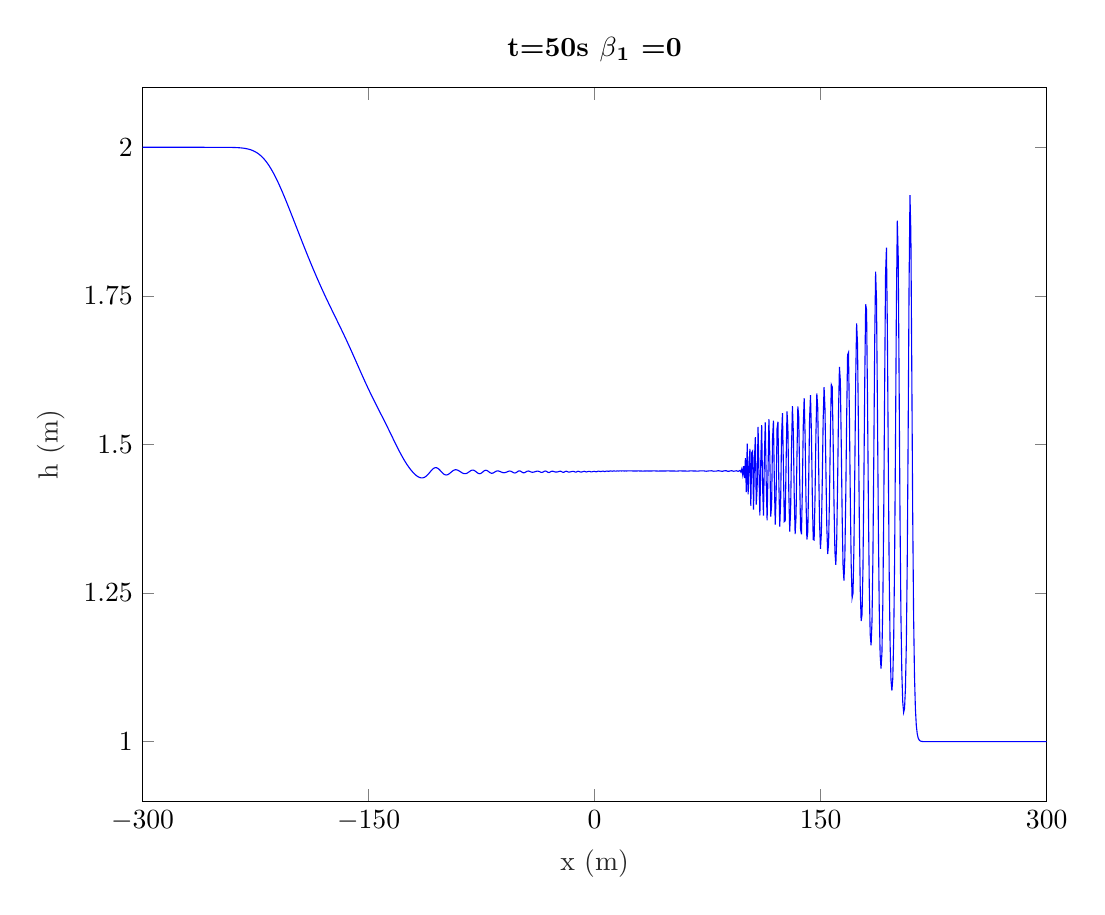
\begin{tikzpicture}

\begin{axis}[%
width=4.521in,
height=3.566in,
at={(0.758in,0.481in)},
scale only axis,
xmin=-300,
xmax=300,
xtick={-300, -150,    0,  150,  300},
xlabel style={font=\color{white!15!black}},
xlabel={x (m)},
ymin=0.9,
ymax=2.1,
ytick={   1, 1.25,  1.5, 1.75,    2},
ylabel style={font=\color{white!15!black}},
ylabel={h (m)},
axis background/.style={fill=white},
title style={font=\bfseries},
title={$\text{t=50s   }\beta{}_\text{1}\text{ =0}$}
]
\addplot [color=blue, forget plot]
  table[row sep=crcr]{%
-300.18000900045	2\\
-299.57997899895	1.99999999999988\\
-298.97994899745	1.99999999999987\\
-298.37991899595	1.99999999999984\\
-297.77988899445	1.9999999999998\\
-297.17985899295	1.99999999999974\\
-296.57982899145	1.99999999999966\\
-295.979798989949	1.99999999999955\\
-295.379768988449	1.99999999999942\\
-294.779738986949	1.99999999999924\\
-294.179708985449	1.99999999999902\\
-293.579678983949	1.99999999999872\\
-292.979648982449	1.99999999999834\\
-292.379618980949	1.99999999999786\\
-291.779588979449	1.99999999999724\\
-291.179558977949	1.99999999999644\\
-290.579528976449	1.99999999999541\\
-289.979498974949	1.99999999999409\\
-289.379468973449	1.9999999999924\\
-288.779438971949	1.99999999999024\\
-288.179408970449	1.99999999998748\\
-287.579378968948	1.99999999998395\\
-286.979348967448	1.99999999997944\\
-286.379318965948	1.99999999997368\\
-285.779288964448	1.99999999996635\\
-285.179258962948	1.999999999957\\
-284.579228961448	1.9999999999451\\
-283.979198959948	1.99999999992996\\
-283.379168958448	1.99999999991073\\
-282.779138956948	1.9999999998863\\
-282.179108955448	1.99999999985531\\
-281.579078953948	1.99999999981603\\
-280.979048952448	1.99999999976627\\
-280.379018950948	1.99999999970331\\
-279.778988949447	1.99999999962369\\
-279.178958947947	1.99999999952312\\
-278.578928946447	1.99999999939617\\
-277.978898944947	1.99999999923609\\
-277.378868943447	1.9999999990344\\
-276.778838941947	1.99999999878051\\
-276.178808940447	1.99999999846121\\
-275.578778938947	1.99999999806002\\
-274.978748937447	1.99999999755641\\
-274.378718935947	1.9999999969248\\
-273.778688934447	1.99999999613344\\
-273.178658932947	1.99999999514286\\
-272.578628931447	1.99999999390409\\
-271.978598929946	1.99999999235646\\
-271.378568928446	1.99999999042487\\
-270.778538926946	1.99999998801643\\
-270.178508925446	1.99999998501643\\
-269.578478923946	1.99999998128334\\
-268.978448922446	1.99999997664276\\
-268.378418920946	1.99999997088001\\
-267.778388919446	1.99999996373119\\
-267.178358917946	1.99999995487219\\
-266.578328916446	1.99999994390554\\
-265.978298914946	1.99999993034436\\
-265.378268913446	1.99999991359292\\
-264.778238911946	1.99999989292335\\
-264.178208910446	1.99999986744735\\
-263.578178908945	1.99999983608227\\
-262.978148907445	1.99999979751031\\
-262.378118905945	1.99999975012957\\
-261.778088904445	1.99999969199538\\
-261.178058902945	1.99999962075021\\
-260.578028901445	1.99999953353993\\
-259.977998899945	1.99999942691406\\
-259.377968898445	1.99999929670706\\
-258.777938896945	1.99999913789739\\
-258.177908895445	1.99999894444048\\
-257.577878893945	1.99999870907112\\
-256.977848892445	1.99999842307011\\
-256.377818890945	1.99999807598931\\
-255.777788889444	1.99999765532836\\
-255.177758887944	1.99999714615524\\
-254.577728886444	1.99999653066197\\
-253.977698884944	1.99999578764555\\
-253.377668883444	1.99999489190281\\
-252.777638881944	1.99999381352665\\
-252.177608880444	1.99999251708945\\
-251.577578878944	1.99999096069816\\
-250.977548877444	1.99998909490332\\
-250.377518875944	1.99998686144318\\
-249.777488874444	1.99998419180164\\
-249.177458872944	1.99998100555733\\
-248.577428871444	1.9999772084991\\
-247.977398869943	1.99997269048141\\
-247.377368868443	1.99996732299174\\
-246.777338866943	1.99996095640032\\
-246.177308865443	1.9999534168619\\
-245.577278863943	1.99994450283804\\
-244.977248862443	1.99993398120876\\
-244.377218860943	1.99992158294262\\
-243.777188859443	1.99990699829596\\
-243.177158857943	1.99988987151419\\
-242.577128856443	1.99986979501217\\
-241.977098854943	1.99984630301534\\
-241.377068853443	1.99981886465063\\
-240.777038851943	1.99978687648448\\
-240.177008850443	1.99974965451624\\
-239.576978848942	1.99970642564858\\
-238.976948847442	1.99965631867164\\
-238.376918845942	1.99959835481627\\
-237.776888844442	1.99953143795221\\
-237.176858842942	1.99945434453045\\
-236.576828841442	1.99936571339488\\
-235.976798839942	1.99926403561626\\
-235.376768838442	1.99914764453115\\
-234.776738836942	1.99901470619924\\
-234.176708835442	1.99886321052351\\
-233.576678833942	1.99869096330794\\
-232.976648832442	1.9984955795558\\
-232.376618830942	1.99827447833625\\
-231.776588829441	1.99802487956684\\
-231.176558827941	1.99774380307217\\
-230.576528826441	1.99742807028321\\
-229.976498824941	1.99707430893496\\
-229.376468823441	1.99667896110121\\
-228.776438821941	1.99623829487168\\
-228.176408820441	1.99574841992869\\
-227.576378818941	1.99520530721521\\
-226.976348817441	1.99460481280565\\
-226.376318815941	1.99394270599353\\
-225.776288814441	1.99321470149957\\
-225.176258812941	1.99241649558081\\
-224.576228811441	1.99154380569041\\
-223.976198809941	1.99059241320272\\
-223.37616880844	1.98955820858479\\
-222.77613880694	1.98843723826862\\
-222.17610880544	1.98722575236565\\
-221.57607880394	1.98592025227186\\
-220.97604880244	1.98451753714421\\
-220.37601880094	1.98301474819278\\
-219.77598879944	1.98140940973217\\
-219.17595879794	1.9796994659719\\
-218.57592879644	1.97788331260135\\
-217.97589879494	1.97595982233703\\
-217.37586879344	1.97392836374735\\
-216.77583879194	1.97178881284559\\
-216.17580879044	1.96954155713991\\
-215.575778788939	1.96718749204105\\
-214.975748787439	1.96472800974421\\
-214.375718785939	1.96216498091352\\
-213.775688784439	1.95950072969451\\
-213.175658782939	1.95673800275475\\
-212.575628781439	1.95387993319852\\
-211.975598779939	1.95093000031161\\
-211.375568778439	1.94789198616501\\
-210.775538776939	1.94476993013966\\
-210.175508775439	1.94156808242875\\
-209.575478773939	1.93829085753371\\
-208.975448772439	1.93494278869722\\
-208.375418770939	1.93152848411861\\
-207.775388769438	1.92805258567878\\
-207.175358767938	1.92451973077091\\
-206.575328766438	1.92093451769564\\
-205.975298764938	1.91730147494111\\
-205.375268763438	1.91362503453535\\
-204.775238761938	1.90990950953483\\
-204.175208760438	1.90615907560221\\
-203.575178758938	1.90237775653082\\
-202.975148757438	1.89856941349493\\
-202.375118755938	1.89473773774323\\
-201.775088754438	1.890886246408\\
-201.175058752938	1.88701828107396\\
-200.575028751438	1.88313700873553\\
-199.974998749937	1.87924542476932\\
-199.374968748437	1.87534635755637\\
-198.774938746937	1.87144247440535\\
-198.174908745437	1.86753628844999\\
-197.574878743937	1.8636301662213\\
-196.974848742437	1.85972633562429\\
-196.374818740937	1.85582689407977\\
-195.774788739437	1.85193381662214\\
-195.174758737937	1.84804896377379\\
-194.574728736437	1.84417408904429\\
-193.974698734937	1.84031084592817\\
-193.374668733437	1.83646079429791\\
-192.774638731937	1.83262540610905\\
-192.174608730437	1.82880607035172\\
-191.574578728936	1.82500409719827\\
-190.974548727436	1.82122072130901\\
-190.374518725936	1.81745710426912\\
-189.774488724436	1.81371433613873\\
-189.174458722936	1.80999343610619\\
-188.574428721436	1.80629535224143\\
-187.974398719936	1.80262096035323\\
-187.374368718436	1.79897106196037\\
-186.774338716936	1.79534638139439\\
-186.174308715436	1.791747562059\\
-185.574278713936	1.78817516188066\\
-184.974248712436	1.78462964799539\\
-184.374218710936	1.78111139072939\\
-183.774188709435	1.77762065694568\\
-183.174158707935	1.77415760284581\\
-182.574128706435	1.77072226633502\\
-181.974098704935	1.76731455908053\\
-181.374068703435	1.76393425841643\\
-180.774038701935	1.76058099927439\\
-180.174008700435	1.75725426634572\\
-179.573978698935	1.75395338670834\\
-178.973948697435	1.75067752317916\\
-178.373918695935	1.74742566867788\\
-177.773888694435	1.74419664191181\\
-177.173858692935	1.74098908470883\\
-176.573828691435	1.73780146133868\\
-175.973798689934	1.73463206016622\\
-175.373768688434	1.73147899797427\\
-174.773738686934	1.72834022727552\\
-174.173708685434	1.72521354690031\\
-173.573678683934	1.72209661610005\\
-172.973648682434	1.71898697234122\\
-172.373618680934	1.71588205288503\\
-171.773588679434	1.7127792201502\\
-171.173558677934	1.70967579074485\\
-170.573528676434	1.70656906792992\\
-169.973498674934	1.70345637714354\\
-169.373468673434	1.70033510408004\\
-168.773438671934	1.69720273468287\\
-168.173408670434	1.69405689628429\\
-167.573378668933	1.69089539901465\\
-166.973348667433	1.6877162765145\\
-166.373318665933	1.68451782492292\\
-165.773288664433	1.68129863908899\\
-165.173258662933	1.67805764496431\\
-164.573228661433	1.67479412718657\\
-163.973198659933	1.67150775095467\\
-163.373168658433	1.66819857742561\\
-162.773138656933	1.66486707202428\\
-162.173108655433	1.66151410524541\\
-161.573078653933	1.65814094573144\\
-160.973048652433	1.65474924562321\\
-160.373018650933	1.65134101839002\\
-159.772988649432	1.64791860954362\\
-159.172958647932	1.64448466081717\\
-158.572928646432	1.6410420685382\\
-157.972898644932	1.63759393703885\\
-157.372868643432	1.63414352802533\\
-156.772838641932	1.63069420687074\\
-156.172808640432	1.62724938680415\\
-155.572778638932	1.62381247194925\\
-154.972748637432	1.62038680012424\\
-154.372718635932	1.61697558625826\\
-153.772688634432	1.61358186721842\\
-153.172658632932	1.61020844878155\\
-152.572628631432	1.60685785543511\\
-151.972598629931	1.60353228365791\\
-151.372568628431	1.60023355931657\\
-150.772538626931	1.59696309982104\\
-150.172508625431	1.59372188170987\\
-149.572478623931	1.59051041438\\
-148.972448622431	1.58732872072971\\
-148.372418620931	1.58417632553757\\
-147.772388619431	1.58105225244312\\
-147.172358617931	1.57795503041239\\
-146.572328616431	1.57488271054946\\
-145.972298614931	1.57183289403826\\
-145.372268613431	1.56880277185422\\
-144.772238611931	1.56578917666273\\
-144.172208610431	1.56278864701367\\
-143.57217860893	1.55979750355021\\
-142.97214860743	1.55681193648085\\
-142.37211860593	1.55382810303505\\
-141.77208860443	1.55084223305607\\
-141.17205860293	1.54785074031508\\
-140.57202860143	1.54485033659591\\
-139.97199859993	1.54183814514283\\
-139.37196859843	1.53881180972866\\
-138.77193859693	1.53576959542438\\
-138.17190859543	1.5327104771673\\
-137.57187859393	1.52963421244859\\
-136.97184859243	1.5265413948757\\
-136.37181859093	1.52343348599689\\
-135.771788589429	1.52031282357079\\
-135.171758587929	1.51718260537818\\
-134.571728586429	1.51404684865018\\
-133.971698584929	1.51091032616583\\
-133.371668583429	1.50777848099392\\
-132.771638581929	1.50465732266962\\
-132.171608580429	1.50155330826855\\
-131.571578578929	1.49847321234964\\
-130.971548577429	1.49542399008254\\
-130.371518575929	1.49241263807022\\
-129.771488574429	1.48944605745147\\
-129.171458572929	1.48653092385832\\
-128.571428571429	1.48367356874811\\
-127.971398569929	1.48087987656162\\
-127.371368568428	1.47815520209732\\
-126.771338566928	1.47550431243988\\
-126.171308565428	1.47293135771634\\
-125.571278563928	1.47043987483157\\
-124.971248562428	1.46803282808388\\
-124.371218560928	1.46571269009099\\
-123.771188559428	1.4634815656597\\
-123.171158557928	1.46134135999704\\
-122.571128556428	1.45929399088129\\
-121.971098554928	1.45734164200257\\
-121.371068553428	1.45548705159189\\
-120.771038551928	1.45373382667696\\
-120.171008550428	1.45208676887841\\
-119.570978548927	1.45055219269319\\
-118.970948547427	1.4491382118633\\
-118.370918545927	1.44785496391482\\
-117.770888544427	1.44671473755819\\
-117.170858542927	1.44573196273316\\
-116.570828541427	1.44492301916723\\
-115.970798539927	1.44430581711484\\
-115.370768538427	1.44389910451379\\
-114.770738536927	1.44372146063014\\
-114.170708535427	1.44378994258984\\
-113.570678533927	1.44411838020962\\
-112.970648532427	1.44471534464606\\
-112.370618530927	1.44558185005082\\
-111.770588529426	1.44670893474905\\
-111.170558527926	1.44807532665505\\
-110.570528526426	1.4496454921484\\
-109.970498524926	1.45136844190847\\
-109.370468523426	1.45317771431355\\
-108.770438521926	1.45499294384506\\
-108.170408520426	1.45672331960477\\
-107.570378518926	1.45827302987675\\
-106.970348517426	1.45954847761402\\
-106.370318515926	1.46046668120492\\
-105.770288514426	1.46096392063557\\
-105.170258512926	1.46100344677215\\
-104.570228511426	1.46058107272695\\
-103.970198509925	1.4597276109491\\
-103.370168508425	1.45850766383628\\
-102.770138506925	1.45701478935074\\
-102.170108505425	1.45536363257791\\
-101.570078503925	1.45368004104419\\
-100.970048502425	1.45209034412089\\
-100.370018500925	1.45071094697687\\
-99.769988499425	1.4496391608232\\
-99.1699584979249	1.44894591562488\\
-98.5699284964248	1.44867071539138\\
-97.9698984949247	1.44881915842567\\
-97.3698684934247	1.44936271740174\\
-96.7698384919246	1.45024148844794\\
-96.1698084904245	1.45136916666492\\
-95.5697784889244	1.45264047365758\\
-94.9697484874244	1.45394046043758\\
-94.3697184859243	1.45515495057142\\
-93.7696884844242	1.45618108335854\\
-93.1696584829241	1.45693672260994\\
-92.5696284814241	1.45736756176637\\
-91.969598479924	1.45745103719943\\
-91.3695684784239	1.45719672974094\\
-90.7695384769239	1.45664346960518\\
-90.1695084754238	1.45585397947451\\
-89.5694784739237	1.45490808218569\\
-88.9694484724236	1.4538955270955\\
-88.3694184709235	1.45290917927555\\
-87.7693884694235	1.45203886361013\\
-87.1693584679234	1.45136573000909\\
-86.5693284664233	1.45095674767048\\
-85.9692984649232	1.45085894914377\\
-85.3692684634232	1.45109331829165\\
-84.7692384619231	1.45164890878735\\
-84.169208460423	1.45247826847365\\
-83.5691784589229	1.45349603709391\\
-82.9691484574229	1.45458270219387\\
-82.3691184559228	1.45559513419377\\
-81.7690884544227	1.45638434056113\\
-81.1690584529227	1.45681894364859\\
-80.5690284514226	1.45681067671174\\
-79.9689984499225	1.45633646210394\\
-79.3689684484224	1.45545105498178\\
-78.7689384469223	1.45428565954109\\
-78.1689084454223	1.45303072252524\\
-77.5688784439222	1.45190483094966\\
-76.9688484424221	1.45111497920343\\
-76.368818440922	1.45081535463275\\
-75.768788439422	1.45107468191087\\
-75.1687584379219	1.45185378261123\\
-74.5687284364218	1.45300877167522\\
-73.9686984349217	1.45431273985213\\
-73.3686684334217	1.45549989228922\\
-72.7686384319216	1.45632265883903\\
-72.1686084304215	1.45660908356702\\
-71.5685784289215	1.4563062820101\\
-70.9685484274214	1.45549368010928\\
-70.3685184259213	1.45436589397498\\
-69.7684884244212	1.45318419685715\\
-69.1684584229211	1.4522128485264\\
-68.5684284214211	1.45165634818382\\
-67.968398419921	1.45161371614262\\
-67.3683684184209	1.45206038759121\\
-66.7683384169208	1.45286104286874\\
-66.1683084154208	1.45380886959004\\
-65.5682784139207	1.45468020581456\\
-64.9682484124206	1.45528944743021\\
-64.3682184109205	1.45552935117231\\
-63.7681884094205	1.45538607547967\\
-63.1681584079204	1.45492988080491\\
-62.5681284064203	1.45428510359186\\
-61.9680984049203	1.45359551937035\\
-61.3680684034202	1.45299443905942\\
-60.7680384019201	1.45258634988048\\
-60.16800840042	1.45243894610592\\
-59.5679783989199	1.45258021489816\\
-58.9679483974199	1.452993426101\\
-58.3679183959198	1.45361113076547\\
-57.7678883944197	1.45431149680976\\
-57.1678583929196	1.45492846528072\\
-56.5678283914196	1.4552836559939\\
-55.9677983899195	1.4552391172248\\
-55.3677683884194	1.45475621416461\\
-54.7677383869193	1.45393495185762\\
-54.1677083854193	1.45300839848694\\
-53.5676783839192	1.45228128787052\\
-52.9676483824191	1.45202622084241\\
-52.3676183809191	1.45237188334835\\
-51.767588379419	1.45323407990821\\
-51.1675583779189	1.45432065301141\\
-50.5675283764188	1.4552288555254\\
-49.9674983749187	1.45560322048735\\
-49.3674683734187	1.45528846158218\\
-48.7674383719186	1.45441204780989\\
-48.1674083704185	1.45333597544751\\
-47.5673783689184	1.45250611793304\\
-46.9673483674184	1.45225848410093\\
-46.3673183659183	1.45267437605519\\
-45.7672883644182	1.45355319339421\\
-45.1672583629181	1.45451201623312\\
-44.5672283614181	1.4551662575078\\
-43.967198359918	1.45529974153615\\
-43.3671683584179	1.45494076285251\\
-42.7671383569178	1.45431352505613\\
-42.1671083554178	1.45370586704453\\
-41.5670783539177	1.45333608610026\\
-40.9670483524176	1.45328780319133\\
-40.3670183509175	1.4535264449351\\
-39.7669883494175	1.45395631212826\\
-39.1669583479174	1.45446197006675\\
-38.5669283464173	1.45491122031328\\
-37.9668983449172	1.45514888563526\\
-37.3668683434172	1.45503249602095\\
-36.7668383419171	1.45452391975202\\
-36.166808340417	1.45377952983385\\
-35.5667783389169	1.45314168713799\\
-34.9667483374168	1.45298102295589\\
-34.3667183359168	1.45345496769956\\
-33.7666883344167	1.45434666158885\\
-33.1666583329167	1.45513592115492\\
-32.5666283314166	1.45530900723734\\
-31.9665983299165	1.45471868532745\\
-31.3665683284164	1.45372096920718\\
-30.7665383269164	1.45295289458108\\
-30.1665083254163	1.45289306678267\\
-29.5664783239162	1.45353237980295\\
-28.9664483224161	1.45440735991598\\
-28.3664183209161	1.45496317047674\\
-27.766388319416	1.45494611640289\\
-27.1663583179159	1.4545123934669\\
-26.5663283164158	1.45401047138384\\
-25.9662983149157	1.45369208956583\\
-25.3662683134157	1.45362201595299\\
-24.7662383119156	1.45378857438638\\
-24.1662083104155	1.45418232658836\\
-23.5661783089154	1.45469744017808\\
-22.9661483074154	1.45502206639585\\
-22.3661183059153	1.45480048318929\\
-21.7660883044152	1.45403256325661\\
-21.1660583029151	1.4532572530331\\
-20.5660283014151	1.45315525487627\\
-19.965998299915	1.45385919214853\\
-19.3659682984149	1.45473310543414\\
-18.7659382969148	1.4549759200553\\
-18.1659082954148	1.45444292215587\\
-17.5658782939147	1.45373491670732\\
-16.9658482924146	1.45347536197706\\
-16.3658182909145	1.45371203424174\\
-15.7657882894144	1.45412360610605\\
-15.1657582879144	1.45451810250125\\
-14.5657282864143	1.45481254247392\\
-13.9656982849143	1.45473812863432\\
-13.3656682834142	1.45412592122312\\
-12.7656382819141	1.45348170783881\\
-12.165608280414	1.4536041701187\\
-11.565578278914	1.45441951354334\\
-10.9655482774139	1.45491149246224\\
-10.3655182759138	1.4545423410954\\
-9.76548827441371	1.45392296280987\\
-9.16545827291367	1.4536721542429\\
-8.56542827141357	1.45372113912215\\
-7.96539826991352	1.45405355742419\\
-7.36536826841342	1.45468230091558\\
-6.76533826691332	1.45486425167201\\
-6.16530826541327	1.45418978936683\\
-5.56527826391317	1.4537147111299\\
-4.96524826241313	1.45407301850106\\
-4.36521826091303	1.45453460484337\\
-3.76518825941298	1.45482706212934\\
-3.16515825791288	1.45477729529384\\
-2.56512825641283	1.45406182756286\\
-1.96509825491273	1.45381511168501\\
-1.36506825341269	1.45429428139124\\
-0.765038251912586	1.45469245131474\\
-0.165008250412541	1.45484965839356\\
0.435021751087561	1.45429484788151\\
1.03505175258761	1.45407151619474\\
1.63508175408771	1.45438096237187\\
2.23511175558775	1.45501860244178\\
2.83514175708785	1.45509822286292\\
3.43517175858796	1.45465087741365\\
4.035201760088	1.45438478261053\\
4.6352317615881	1.45475124435944\\
5.23526176308815	1.455208463828\\
5.83529176458825	1.45504660253011\\
6.43532176608829	1.45454466862316\\
7.03535176758839	1.45455885720779\\
7.63538176908844	1.45510924309853\\
8.23541177058854	1.45531123573671\\
8.83544177208859	1.45492748611237\\
9.43547177358869	1.45480738808618\\
10.0355017750887	1.45531616580636\\
10.6355317765888	1.45559417358522\\
11.2355617780889	1.45518845631408\\
11.835591779589	1.4550040983826\\
12.435621781089	1.45543967031173\\
13.0356517825891	1.45551920551673\\
13.6356817840892	1.455056551333\\
14.2357117855893	1.45512881300433\\
14.8357417870894	1.45558533414975\\
15.4357717885894	1.45539050007359\\
16.0358017900895	1.45520272607218\\
16.6358317915896	1.45566457799074\\
17.2358617930897	1.4556364729309\\
17.8358917945897	1.45531170215369\\
18.4359217960898	1.45564655847095\\
19.0359517975899	1.45553013004801\\
19.63598179909	1.45524755980212\\
20.23601180059	1.45557280603069\\
20.8360418020901	1.45531502390911\\
21.4360718035902	1.45542866821189\\
22.0361018050903	1.45551812686398\\
22.6361318065904	1.45546041250732\\
23.2361618080904	1.45560126855701\\
23.8361918095905	1.45551836701294\\
24.4362218110905	1.45551479808694\\
25.0362518125906	1.45545477288113\\
25.6362818140907	1.45539519496568\\
26.2363118155908	1.45536152642667\\
26.8363418170908	1.45535134039177\\
27.4363718185909	1.45537958577963\\
28.036401820091	1.45542645184143\\
28.6364318215911	1.45546358674266\\
29.2364618230911	1.45546909337234\\
29.8364918245912	1.45543679882338\\
30.4365218260913	1.455378067505\\
31.0365518275914	1.45531541306787\\
31.6365818290914	1.45527135251764\\
32.2366118305915	1.45526369364631\\
32.8366418320916	1.45530103939821\\
33.4366718335917	1.45536674801477\\
34.0367018350918	1.45543192191173\\
34.6367318365918	1.45546618006332\\
35.2367618380919	1.45544737175912\\
35.836791839592	1.45540269056228\\
36.4368218410921	1.45535626188545\\
37.0368518425921	1.45534601287505\\
37.6368818440922	1.45538852164369\\
38.2369118455923	1.45545470886232\\
38.8369418470924	1.45551347376148\\
39.4369718485924	1.45553560414038\\
40.0370018500925	1.45549764457863\\
40.6370318515926	1.45541472084791\\
41.2370618530927	1.45532933358776\\
41.8370918545928	1.45527457039853\\
42.4371218560928	1.4552672088301\\
43.0371518575929	1.45530596973024\\
43.6371818590929	1.4553597148038\\
44.237211860593	1.45538279220424\\
44.8372418620931	1.45535646863761\\
45.4372718635932	1.45530560881744\\
46.0373018650932	1.4552760405841\\
46.6373318665933	1.45530220768486\\
47.2373618680934	1.45538668273206\\
47.8373918695935	1.45549378911605\\
48.4374218710935	1.45556292811835\\
49.0374518725936	1.45554739656653\\
49.6374818740937	1.45545365926823\\
50.2375118755938	1.4553421021732\\
50.8375418770938	1.45528090133901\\
51.4375718785939	1.45529171247522\\
52.037601880094	1.45533523075393\\
52.6376318815941	1.45534840980302\\
53.2376618830942	1.455301534753\\
53.8376918845942	1.45522722703985\\
54.4377218860943	1.4551968336758\\
55.0377518875944	1.45526041479686\\
55.6377818890945	1.45539830827242\\
56.2378118905945	1.45552785757753\\
56.8378418920946	1.45556661623168\\
57.4378718935947	1.45550188048137\\
58.0379018950948	1.45540167626761\\
58.6379318965948	1.45535110051412\\
59.2379618980949	1.45536907532104\\
59.837991899595	1.45539031986971\\
60.4380219010951	1.45533892711602\\
61.0380519025952	1.45522328965748\\
61.6380819040952	1.45514792258501\\
62.2381119055953	1.45521392877328\\
62.8381419070953	1.45540254816842\\
63.4381719085955	1.45557611077416\\
64.0382019100955	1.45560995393419\\
64.6382319115956	1.45552036140619\\
65.2382619130956	1.45543671932126\\
65.8382919145957	1.45543906976615\\
66.4383219160958	1.45545523501452\\
67.0383519175959	1.45536163056312\\
67.6383819190959	1.45517457135234\\
68.238411920596	1.4550757024028\\
68.8384419220961	1.45520019915811\\
69.4384719235962	1.4554476300584\\
70.0385019250962	1.45558818530491\\
70.6385319265963	1.45555351762427\\
71.2385619280964	1.45550538461254\\
71.8385919295965	1.45555704223497\\
72.4386219310966	1.45556338346041\\
73.0386519325966	1.45534611121456\\
73.6386819340967	1.45504690327486\\
74.2387119355968	1.45499930499563\\
74.8387419370969	1.45523868136382\\
75.4387719385969	1.45544610446071\\
76.038801940097	1.45547791645981\\
76.6388319415971	1.45556162617876\\
77.2388619430972	1.45574827387654\\
77.8388919445972	1.45567675918603\\
78.4389219460973	1.45525712012717\\
79.0389519475974	1.45498577210841\\
79.6389819490975	1.45509352432236\\
80.2390119505975	1.4551885663101\\
80.8390419520976	1.45523300870514\\
81.4390719535977	1.45560419673903\\
82.0391019550977	1.4559302577976\\
82.6391319565979	1.45564736671277\\
83.2391619580979	1.45530235894671\\
83.839191959598	1.45520759736504\\
84.439221961098	1.45487588692137\\
85.0392519625981	1.45490116141803\\
85.6392819640982	1.45552357076202\\
86.2393119655983	1.45567118307129\\
86.8393419670983	1.45581774079207\\
87.4393719685984	1.45572540551411\\
88.0394019700985	1.45503563325847\\
88.6394319715986	1.45499141381237\\
89.2394619730986	1.45487191002626\\
89.8394919745987	1.45547316064392\\
90.4395219760988	1.45572511159896\\
91.0395519775989	1.45580369702692\\
91.639581979099	1.45532796724567\\
92.239611980599	1.45498306758108\\
92.8396419820991	1.45508510623607\\
93.4396719835992	1.45555141016533\\
94.0397019850993	1.45573298741601\\
94.6397319865993	1.45532505434633\\
95.2397619880994	1.45483623512699\\
95.8397919895995	1.45541996123949\\
96.4398219910996	1.45622936723046\\
97.0398519925996	1.45364084092931\\
97.6398819940997	1.45887042548994\\
98.2399119955998	1.44918204381578\\
98.8399419970999	1.46342321659656\\
99.4399719985999	1.44328070868586\\
100.0400020001	1.47701324010203\\
100.6400320016	1.41974788576736\\
101.2400620031	1.50142745180945\\
101.8400920046	1.41622197709425\\
102.4401220061	1.4628576276857\\
103.0401520076	1.49267575719867\\
103.6401820091	1.3966329041084\\
104.240212010601	1.48622002341338\\
104.840242012101	1.48891739718163\\
105.440272013601	1.39044416742851\\
106.040302015101	1.47462966759951\\
106.640332016601	1.51246718280575\\
107.240362018101	1.39892263203878\\
107.840392019601	1.42694785959626\\
108.440422021101	1.52958796557111\\
109.040452022601	1.45574127195947\\
109.640482024101	1.38051027166247\\
110.240512025601	1.47156936505347\\
110.840542027101	1.53269413259328\\
111.440572028601	1.42910361872935\\
112.040602030102	1.38013812432788\\
112.640632031602	1.47975709728327\\
113.240662033102	1.53711635390346\\
113.840692034602	1.43781318062555\\
114.440722036102	1.37246287295104\\
115.040752037602	1.45267435786454\\
115.640782039102	1.54269461926189\\
116.240812040602	1.48144388472486\\
116.840842042102	1.37882107041481\\
117.440872043602	1.3977021779497\\
118.040902045102	1.50955057315633\\
118.640932046602	1.54004086420332\\
119.240962048102	1.43955481931228\\
119.840992049603	1.36535195349796\\
120.441022051103	1.41679498630451\\
121.041052052603	1.52678153213582\\
121.641082054103	1.53815030608114\\
122.241112055603	1.43470213168251\\
122.841142057103	1.36181076684655\\
123.441172058603	1.40539954191816\\
124.041202060103	1.51564375358021\\
124.641232061603	1.55264777839331\\
125.241262063103	1.46580696550558\\
125.841292064603	1.37024053973901\\
126.441322066103	1.37151223195234\\
127.041352067603	1.46747759870124\\
127.641382069103	1.55546174733646\\
128.241412070604	1.52771784598735\\
128.841442072104	1.42031156204777\\
129.441472073604	1.35351968425863\\
130.041502075104	1.38775012421172\\
130.641532076604	1.49280074957538\\
131.241562078104	1.56446263368118\\
131.841592079604	1.52140834426837\\
132.441622081104	1.41407107795399\\
133.041652082604	1.34919329445461\\
133.641682084104	1.37802124118954\\
134.241712085604	1.47868951052121\\
134.841742087104	1.56402562197393\\
135.441772088604	1.5463115409004\\
136.041802090105	1.4450597592163\\
136.641832091605	1.35720828458546\\
137.241862093105	1.34885053420499\\
137.841892094605	1.42502152562889\\
138.441922096105	1.53232949105083\\
139.041952097605	1.57776659288601\\
139.641982099105	1.51631604044934\\
140.242012100605	1.4082828740442\\
140.842042102105	1.34015545205983\\
141.442072103605	1.3532603181004\\
142.042102105105	1.43986823594352\\
142.642132106605	1.54457424121162\\
143.242162108105	1.58314286994019\\
143.842192109605	1.52058697341286\\
144.442222111106	1.41358632037078\\
145.042252112606	1.33999525441197\\
145.642282114106	1.33917336826103\\
146.242312115606	1.41073379859949\\
146.842342117106	1.51706804102183\\
147.442372118606	1.58612275267009\\
148.042402120106	1.5618058684002\\
148.642432121606	1.46551337475543\\
149.242462123106	1.36853305351848\\
149.842492124606	1.32432172469888\\
150.442522126106	1.35043600154861\\
151.042552127606	1.4365772135104\\
151.642582129106	1.54109459048537\\
152.242612130607	1.59656187241738\\
152.842642132107	1.56046696776617\\
153.442672133607	1.46100036628035\\
154.042702135107	1.36386162998003\\
154.642732136607	1.31575506217163\\
155.242762138107	1.33307092104272\\
155.842792139607	1.41097200259098\\
156.442822141107	1.51994932490701\\
157.042852142607	1.60080306093407\\
157.642882144107	1.59695891952244\\
158.242912145607	1.51051829181017\\
158.842942147107	1.39912065221087\\
159.442972148607	1.31910080537846\\
160.043002150107	1.29751667533318\\
160.643032151608	1.34041172409407\\
161.243062153108	1.43855720573606\\
161.843092154608	1.55681932392168\\
162.443122156108	1.63049691415818\\
163.043152157608	1.60729496576173\\
163.643182159108	1.50240464045797\\
164.243212160608	1.3806516907977\\
164.843242162108	1.29590324351411\\
165.443272163608	1.27090615895289\\
166.043302165108	1.31112296529533\\
166.643332166608	1.41193665337072\\
167.243362168108	1.54641737795818\\
167.843392169608	1.65065962046536\\
168.443422171109	1.65465439352996\\
169.043452172609	1.55326310332985\\
169.643482174109	1.41215361044467\\
170.243512175609	1.29817892243241\\
170.843542177109	1.24166045846569\\
171.443572178609	1.24975765786803\\
172.043602180109	1.32400475954467\\
172.643632181609	1.45737870998939\\
173.243662183109	1.61113598147605\\
173.843692184609	1.70389833498805\\
174.443722186109	1.66844033542466\\
175.043752187609	1.52899074014354\\
175.643782189109	1.37083806116676\\
176.24381219061	1.25588037347454\\
176.84384219211	1.20303742862175\\
177.44387219361	1.21361619191501\\
178.04390219511	1.28980007772296\\
178.64393219661	1.43100746082144\\
179.24396219811	1.60746713851101\\
179.84399219961	1.73585897510924\\
180.44402220111	1.72623166527824\\
181.04405220261	1.58410265678509\\
181.64408220411	1.40299525606135\\
182.24411220561	1.26064310187236\\
182.84414220711	1.18097613047313\\
183.44417220861	1.16183912302514\\
184.04420221011	1.2018046982215\\
184.644232211611	1.30708421204848\\
185.244262213111	1.47793789656542\\
185.844292214611	1.67332279850113\\
186.444322216111	1.79061992749058\\
187.044352217611	1.74223368133464\\
187.644382219111	1.56451694455072\\
188.244412220611	1.36893574126115\\
188.844442222111	1.22578850983501\\
189.444472223611	1.14687703092809\\
190.044502225111	1.12299423131512\\
190.644532226611	1.14953448462001\\
191.244562228111	1.23349355178256\\
191.844592229611	1.38651445328054\\
192.444622231112	1.59683610256499\\
193.044652232612	1.78651615692953\\
193.644682234112	1.8313169775266\\
194.244712235612	1.69439881448428\\
194.844742237112	1.47665944980039\\
195.444772238612	1.28817643949615\\
196.044802240112	1.16659414551368\\
196.644832241612	1.10401274858035\\
197.244862243112	1.08571572787303\\
197.844892244612	1.10630373256543\\
198.444922246112	1.17305036342873\\
199.044952247612	1.30287342922191\\
199.644982249112	1.50487756509175\\
200.245012250613	1.73694341550793\\
200.845042252113	1.87654006436205\\
201.445072253613	1.8162318481952\\
202.045102255113	1.6044132079555\\
202.645132256613	1.37744910170838\\
203.245162258113	1.21288795465589\\
203.845192259613	1.11586617678756\\
204.445222261113	1.06685920706157\\
205.045252262613	1.04921450842379\\
205.645282264113	1.0559040560893\\
206.245312265613	1.09007796345857\\
206.845342267113	1.1653737236076\\
207.445372268613	1.30368490971133\\
208.045402270114	1.51827753021783\\
208.645432271614	1.76734180548004\\
209.245462273114	1.91936708371987\\
209.845492274614	1.85580371037024\\
210.445522276114	1.62905040445733\\
211.045552277614	1.38770628144333\\
211.645582279114	1.2139980962898\\
212.245612280614	1.11105754004387\\
212.845642282114	1.05580738782781\\
213.445672283614	1.02759175944844\\
214.045702285114	1.01353251434736\\
214.645732286614	1.00661108895807\\
215.245762288114	1.00322361316498\\
215.845792289614	1.00157043320625\\
216.445822291115	1.00076473911612\\
217.045852292615	1.00037232931089\\
217.645882294115	1.00018126394138\\
218.245912295615	1.00008824506511\\
218.845942297115	1.00004296119116\\
219.445972298615	1.00002091582801\\
220.046002300115	1.00001018332722\\
220.646032301615	1.00000495817459\\
221.246062303115	1.00000241419477\\
221.846092304615	1.00000117555166\\
222.446122306115	1.00000057244064\\
223.046152307615	1.00000027876538\\
223.646182309115	1.00000013575853\\
224.246212310616	1.00000006611738\\
224.846242312116	1.00000003220212\\
225.446272313616	1.00000001568462\\
226.046302315116	1.00000000763985\\
226.646332316616	1.00000000372148\\
227.246362318116	1.00000000181288\\
227.846392319616	1.00000000088316\\
228.446422321116	1.00000000043027\\
229.046452322616	1.00000000020963\\
229.646482324116	1.00000000010213\\
230.246512325616	1.00000000004976\\
230.846542327116	1.00000000002425\\
231.446572328616	1.00000000001181\\
232.046602330116	1.00000000000575\\
232.646632331617	1.0000000000028\\
233.246662333117	1.00000000000136\\
233.846692334617	1.00000000000066\\
234.446722336117	1.00000000000032\\
235.046752337617	1.00000000000015\\
235.646782339117	1.00000000000007\\
236.246812340617	1.00000000000003\\
236.846842342117	1.00000000000001\\
237.446872343617	1\\
238.046902345117	1\\
238.646932346617	1\\
239.246962348117	1\\
239.846992349617	1\\
240.447022351118	1\\
241.047052352618	1\\
241.647082354118	1\\
242.247112355618	1\\
242.847142357118	1\\
243.447172358618	1\\
244.047202360118	1\\
244.647232361618	1\\
245.247262363118	1\\
245.847292364618	1\\
246.447322366118	1\\
247.047352367618	1\\
247.647382369118	1\\
248.247412370619	1\\
248.847442372119	1\\
249.447472373619	1\\
250.047502375119	1\\
250.647532376619	1\\
251.247562378119	1\\
251.847592379619	1\\
252.447622381119	1\\
253.047652382619	1\\
253.647682384119	1\\
254.247712385619	1\\
254.847742387119	1\\
255.447772388619	1\\
256.04780239012	1\\
256.64783239162	1\\
257.24786239312	1\\
257.84789239462	1\\
258.44792239612	1\\
259.04795239762	1\\
259.64798239912	1\\
260.24801240062	1\\
260.84804240212	1\\
261.44807240362	1\\
262.04810240512	1\\
262.64813240662	1\\
263.24816240812	1\\
263.84819240962	1\\
264.448222411121	1\\
265.048252412621	1\\
265.648282414121	1\\
266.248312415621	1\\
266.848342417121	1\\
267.448372418621	1\\
268.048402420121	1\\
268.648432421621	1\\
269.248462423121	1\\
269.848492424621	1\\
270.448522426121	1\\
271.048552427621	1\\
271.648582429121	1\\
272.248612430622	1\\
272.848642432122	1\\
273.448672433622	1\\
274.048702435122	1\\
274.648732436622	1\\
275.248762438122	1\\
275.848792439622	1\\
276.448822441122	1\\
277.048852442622	1\\
277.648882444122	1\\
278.248912445622	1\\
278.848942447122	1\\
279.448972448622	1\\
280.049002450123	1\\
280.649032451623	1\\
281.249062453123	1\\
281.849092454623	1\\
282.449122456123	1\\
283.049152457623	1\\
283.649182459123	1\\
284.249212460623	1\\
284.849242462123	1\\
285.449272463623	1\\
286.049302465123	1\\
286.649332466623	1\\
287.249362468123	1\\
287.849392469623	1\\
288.449422471124	1\\
289.049452472624	1\\
289.649482474124	1\\
290.249512475624	1\\
290.849542477124	1\\
291.449572478624	1\\
292.049602480124	1\\
292.649632481624	1\\
293.249662483124	1\\
293.849692484624	1\\
294.449722486124	1\\
295.049752487624	1\\
295.649782489125	1\\
296.249812490625	1\\
296.849842492125	1\\
297.449872493625	1\\
298.049902495125	1\\
298.649932496625	1\\
299.249962498125	1\\
299.849992499625	1\\
};
\end{axis}
\end{tikzpicture}%
	\caption{$t=50s$}
	\end{subfigure}
	\begin{subfigure}{0.49\textwidth}
	\centering
	% This file was created by matlab2tikz.
%
%The latest updates can be retrieved from
%  http://www.mathworks.com/matlabcentral/fileexchange/22022-matlab2tikz-matlab2tikz
%where you can also make suggestions and rate matlab2tikz.
%
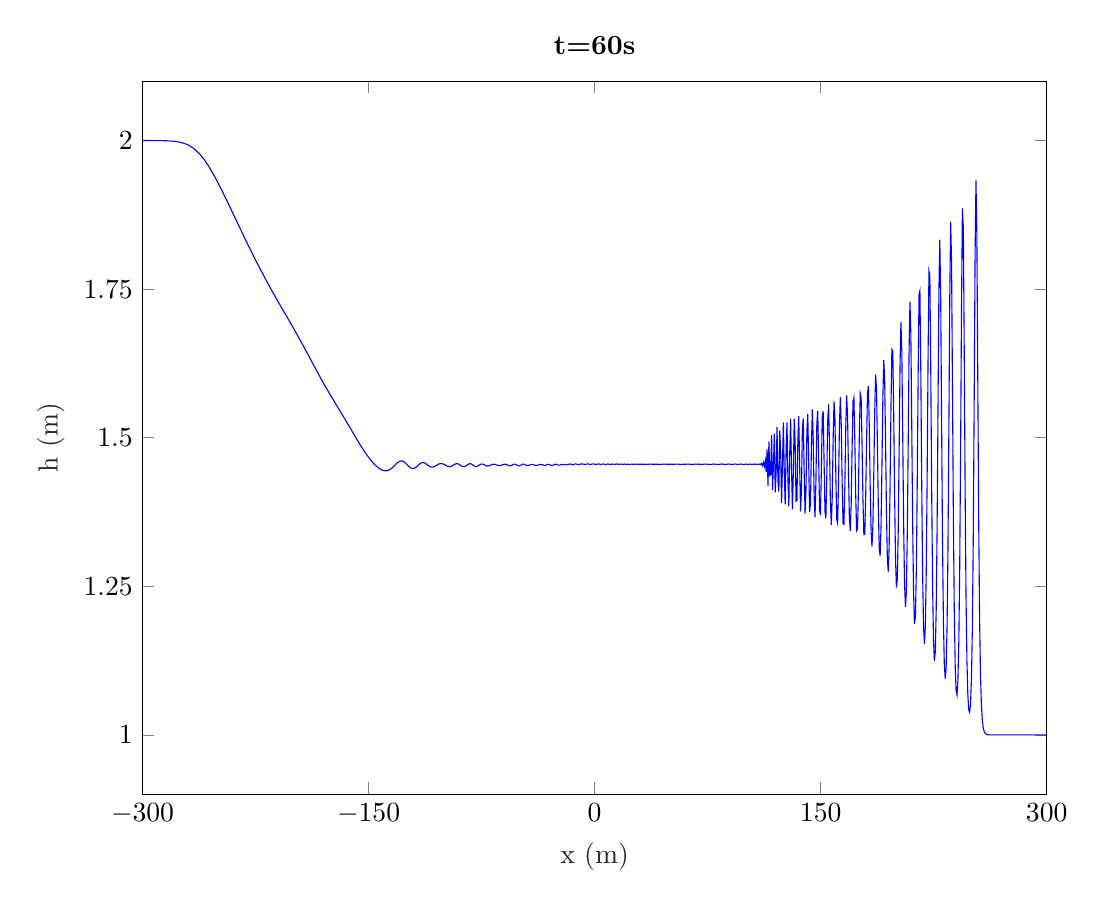
\begin{tikzpicture}

\begin{axis}[%
width=4.521in,
height=3.566in,
at={(0.758in,0.481in)},
scale only axis,
xmin=-300,
xmax=300,
xtick={-300, -150,    0,  150,  300},
xlabel style={font=\color{white!15!black}},
xlabel={x (m)},
ymin=0.9,
ymax=2.1,
ytick={   1, 1.25,  1.5, 1.75,    2},
ylabel style={font=\color{white!15!black}},
ylabel={h (m)},
axis background/.style={fill=white},
title style={font=\bfseries},
title={t=60s}
]
\addplot [color=blue, forget plot]
  table[row sep=crcr]{%
-300.18000900045	2\\
-299.57997899895	1.99998842512532\\
-298.97994899745	1.99998787096171\\
-298.37991899595	1.99998697001826\\
-297.77988899445	1.9999856841661\\
-297.17985899295	1.99998398101269\\
-296.57982899145	1.99998181810856\\
-295.979798989949	1.99997914214306\\
-295.379768988449	1.99997588796482\\
-294.779738986949	1.99997197740754\\
-294.179708985449	1.99996731791092\\
-293.579678983949	1.99996180092605\\
-292.979648982449	1.9999553000931\\
-292.379618980949	1.99994766917921\\
-291.779588979449	1.99993873976409\\
-291.179558977949	1.99992831866085\\
-290.579528976449	1.99991618506064\\
-289.979498974949	1.99990208739045\\
-289.379468973449	1.99988573987552\\
-288.779438971949	1.99986681880009\\
-288.179408970449	1.99984495846367\\
-287.579378968948	1.9998197468338\\
-286.979348967448	1.99979072090183\\
-286.379318965948	1.99975736175359\\
-285.779288964448	1.99971908937472\\
-285.179258962948	1.99967525721792\\
-284.579228961448	1.99962514656929\\
-283.979198959948	1.99956796076097\\
-283.379168958448	1.9995028192889\\
-282.779138956948	1.9994287519072\\
-282.179108955448	1.99934469278333\\
-281.579078953948	1.99924947481263\\
-280.979048952448	1.99914182420442\\
-280.379018950948	1.99902035546615\\
-279.778988949447	1.99888356692528\\
-279.178958947947	1.99872983694151\\
-278.578928946447	1.99855742097205\\
-277.978898944947	1.99836444966211\\
-277.378868943447	1.99814892813738\\
-276.778838941947	1.997908736678\\
-276.178808940447	1.99764163295036\\
-275.578778938947	1.99734525596546\\
-274.978748937447	1.99701713191931\\
-274.378718935947	1.99665468205055\\
-273.778688934447	1.99625523262415\\
-273.178658932947	1.99581602711687\\
-272.578628931447	1.99533424063959\\
-271.978598929946	1.99480699658557\\
-271.378568928446	1.99423138544145\\
-270.778538926946	1.99360448564106\\
-270.178508925446	1.99292338628269\\
-269.578478923946	1.99218521146909\\
-268.978448922446	1.99138714596926\\
-268.378418920946	1.99052646184351\\
-267.778388919446	1.98960054562156\\
-267.178358917946	1.98860692557889\\
-266.578328916446	1.98754329862291\\
-265.978298914946	1.98640755627877\\
-265.378268913446	1.98519780925703\\
-264.778238911946	1.98391241009322\\
-264.178208910446	1.98254997337321\\
-263.578178908945	1.98110939309812\\
-262.978148907445	1.97958985679734\\
-262.378118905945	1.97799085606755\\
-261.778088904445	1.97631219329566\\
-261.178058902945	1.97455398441332\\
-260.578028901445	1.97271665762571\\
-259.977998899945	1.97080094815447\\
-259.377968898445	1.96880788913056\\
-258.777938896945	1.96673879886358\\
-258.177908895445	1.96459526479649\\
-257.577878893945	1.96237912452596\\
-256.977848892445	1.96009244432603\\
-256.377818890945	1.95773749565548\\
-255.777788889444	1.95531673015559\\
-255.177758887944	1.95283275365495\\
-254.577728886444	1.95028829969263\\
-253.977698884944	1.94768620305066\\
-253.377668883444	1.94502937375404\\
-252.777638881944	1.94232077195254\\
-252.177608880444	1.93956338404695\\
-251.577578878944	1.93676020036445\\
-250.977548877444	1.93391419462684\\
-250.377518875944	1.93102830539358\\
-249.777488874444	1.92810541960085\\
-249.177458872944	1.92514835826035\\
-248.577428871444	1.92215986432902\\
-247.977398869943	1.91914259271352\\
-247.377368868443	1.91609910233308\\
-246.777338866943	1.91303185013094\\
-246.177308865443	1.90994318689814\\
-245.577278863943	1.90683535475415\\
-244.977248862443	1.90371048611583\\
-244.377218860943	1.90057060397946\\
-243.777188859443	1.89741762333857\\
-243.177158857943	1.89425335356347\\
-242.577128856443	1.89107950157446\\
-241.977098854943	1.88789767565052\\
-241.377068853443	1.88470938972619\\
-240.777038851943	1.88151606804303\\
-240.177008850443	1.87831905003515\\
-239.576978848942	1.87511959534308\\
-238.976948847442	1.87191888886358\\
-238.376918845942	1.86871804575721\\
-237.776888844442	1.86551811634751\\
-237.176858842942	1.86232009085791\\
-236.576828841442	1.85912490394299\\
-235.976798839942	1.85593343898021\\
-235.376768838442	1.85274653209664\\
-234.776738836942	1.84956497591225\\
-234.176708835442	1.84638952298759\\
-233.576678833942	1.84322088896835\\
-232.976648832442	1.84005975542362\\
-232.376618830942	1.83690677237767\\
-231.776588829441	1.83376256053736\\
-231.176558827941	1.83062771321919\\
-230.576528826441	1.82750279798125\\
-229.976498824941	1.8243883579655\\
-229.376468823441	1.82128491295701\\
-228.776438821941	1.818192960166\\
-228.176408820441	1.81511297473909\\
-227.576378818941	1.81204541000547\\
-226.976348817441	1.80899069746372\\
-226.376318815941	1.8059492465146\\
-225.776288814441	1.80292144394514\\
-225.176258812941	1.79990765316906\\
-224.576228811441	1.79690821322909\\
-223.976198809941	1.79392343756688\\
-223.37616880844	1.79095361256703\\
-222.77613880694	1.78799899588274\\
-222.17610880544	1.78505981455213\\
-221.57607880394	1.78213626291575\\
-220.97604880244	1.77922850034855\\
-220.37601880094	1.77633664882153\\
-219.77598879944	1.77346079031231\\
-219.17595879794	1.77060096408662\\
-218.57592879644	1.76775716387746\\
-217.97589879494	1.7649293349928\\
-217.37586879344	1.76211737138782\\
-216.77583879194	1.75932111274297\\
-216.17580879044	1.75654034159453\\
-215.575778788939	1.75377478057052\\
-214.975748787439	1.75102408978993\\
-214.375718785939	1.74828786448973\\
-213.775688784439	1.74556563294882\\
-213.175658782939	1.74285685478333\\
-212.575628781439	1.74016091969172\\
-211.975598779939	1.73747714673123\\
-211.375568778439	1.73480478420885\\
-210.775538776939	1.73214301027051\\
-210.175508775439	1.72949093427001\\
-209.575478773939	1.72684759899564\\
-208.975448772439	1.72421198382573\\
-208.375418770939	1.72158300887548\\
-207.775388769438	1.71895954018534\\
-207.175358767938	1.71634039598625\\
-206.575328766438	1.71372435405938\\
-205.975298764938	1.71111016018722\\
-205.375268763438	1.70849653766963\\
-204.775238761938	1.7058821978532\\
-204.175208760438	1.7032658515954\\
-203.575178758938	1.70064622155664\\
-202.975148757438	1.69802205518578\\
-202.375118755938	1.69539213823719\\
-201.775088754438	1.69275530863159\\
-201.175058752938	1.69011047045078\\
-200.575028751438	1.68745660783707\\
-199.974998749937	1.6847927985542\\
-199.374968748437	1.68211822695831\\
-198.774938746937	1.67943219612523\\
-198.174908745437	1.67673413888537\\
-197.574878743937	1.67402362752922\\
-196.974848742437	1.67130038196523\\
-196.374818740937	1.66856427613747\\
-195.774788739437	1.66581534254177\\
-195.174758737937	1.66305377471542\\
-194.574728736437	1.66027992761569\\
-193.974698734937	1.65749431584523\\
-193.374668733437	1.6546976097257\\
-192.774638731937	1.65189062926414\\
-192.174608730437	1.64907433609722\\
-191.574578728936	1.646249823536\\
-190.974548727436	1.64341830486628\\
-190.374518725936	1.64058110008676\\
-189.774488724436	1.63773962128768\\
-189.174458722936	1.63489535688699\\
-188.574428721436	1.63204985494833\\
-187.974398719936	1.62920470580655\\
-187.374368718436	1.62636152422198\\
-186.774338716936	1.6235219312757\\
-186.174308715436	1.62068753620519\\
-185.574278713936	1.6178599183647\\
-184.974248712436	1.61504060947824\\
-184.374218710936	1.61223107633689\\
-183.774188709435	1.60943270407743\\
-183.174158707935	1.60664678016645\\
-182.574128706435	1.60387447920552\\
-181.974098704935	1.60111684866712\\
-181.374068703435	1.59837479567098\\
-180.774038701935	1.59564907491363\\
-180.174008700435	1.59294027787233\\
-179.573978698935	1.59024882341615\\
-178.973948697435	1.58757494997203\\
-178.373918695935	1.58491870940961\\
-177.773888694435	1.58227996282597\\
-177.173858692935	1.5796583784264\\
-176.573828691435	1.57705343170935\\
-175.973798689934	1.57446440817003\\
-175.373768688434	1.5718904087361\\
-174.773738686934	1.56933035813756\\
-174.173708685434	1.56678301639033\\
-173.573678683934	1.56424699353706\\
-172.973648682434	1.56172076773782\\
-172.373618680934	1.55920270673857\\
-171.773588679434	1.55669109266475\\
-171.173558677934	1.55418414999491\\
-170.573528676434	1.55168007646483\\
-169.973498674934	1.54917707654179\\
-169.373468673434	1.54667339699357\\
-168.773438671934	1.54416736396512\\
-168.173408670434	1.54165742087147\\
-167.573378668933	1.53914216632603\\
-166.973348667433	1.53662039125434\\
-166.373318665933	1.5340911143007\\
-165.773288664433	1.53155361462338\\
-165.173258662933	1.52900746119667\\
-164.573228661433	1.52645253779629\\
-163.973198659933	1.52388906293815\\
-163.373168658433	1.52131760416654\\
-162.773138656933	1.5187390862412\\
-162.173108655433	1.51615479294799\\
-161.573078653933	1.51356636244575\\
-160.973048652433	1.51097577625487\\
-160.373018650933	1.5083853421816\\
-159.772988649432	1.50579767164795\\
-159.172958647932	1.50321565205395\\
-158.572928646432	1.50064241492965\\
-157.972898644932	1.49808130073836\\
-157.372868643432	1.49553582126582\\
-156.772838641932	1.49300962057656\\
-156.172808640432	1.4905064355399\\
-155.572778638932	1.48803005693052\\
-154.972748637432	1.48558429209626\\
-154.372718635932	1.48317293016806\\
-153.772688634432	1.48079971076735\\
-153.172658632932	1.47846829715123\\
-152.572628631432	1.47618225472849\\
-151.972598629931	1.47394503588078\\
-151.372568628431	1.47175997203057\\
-150.772538626931	1.46963027390572\\
-150.172508625431	1.46755904094907\\
-149.572478623931	1.46554928079773\\
-148.972448622431	1.46360393969091\\
-148.372418620931	1.4617259445369\\
-147.772388619431	1.45991825715132\\
-147.172358617931	1.458183940842\\
-146.572328616431	1.4565262390284\\
-145.972298614931	1.45494866491257\\
-145.372268613431	1.45345510033207\\
-144.772238611931	1.45204990079133\\
-144.172208610431	1.45073800226312\\
-143.57217860893	1.44952502365704\\
-142.97214860743	1.44841735686564\\
-142.37211860593	1.44742223403756\\
-141.77208860443	1.44654775924225\\
-141.17205860293	1.44580288907979\\
-140.57202860143	1.44519734422079\\
-139.97199859993	1.44474143160349\\
-139.37196859843	1.44444575547205\\
-138.77193859693	1.444320797469\\
-138.17190859543	1.44437633154673\\
-137.57187859393	1.4446206955928\\
-136.97184859243	1.4450598576714\\
-136.37181859093	1.44569633711042\\
-135.771788589429	1.44652798120119\\
-135.171758587929	1.4475466651701\\
-134.571728586429	1.4487370078008\\
-133.971698584929	1.45007523501798\\
-133.371668583429	1.45152836171926\\
-132.771638581929	1.4530538908348\\
-132.171608580429	1.45460023762994\\
-131.571578578929	1.45610806485658\\
-130.971548577429	1.45751265051225\\
-130.371518575929	1.45874730076234\\
-129.771488574429	1.45974767191397\\
-129.171458572929	1.46045669652649\\
-128.571428571429	1.4608296511071\\
-127.971398569929	1.46083879019891\\
-127.371368568428	1.4604769787945\\
-126.771338566928	1.45975975086408\\
-126.171308565428	1.45872552699534\\
-125.571278563928	1.45743384235641\\
-124.971248562428	1.45596177924399\\
-124.371218560928	1.45439895674713\\
-123.771188559428	1.45284159718183\\
-123.171158557928	1.45138620336811\\
-122.571128556428	1.45012332449734\\
-121.971098554928	1.44913178916085\\
-121.371068553428	1.44847364784904\\
-120.771038551928	1.44818999925459\\
-120.171008550428	1.44829780493238\\
-119.570978548927	1.44878786640158\\
-118.970948547427	1.44962415561549\\
-118.370918545927	1.45074479375504\\
-117.770888544427	1.45206497761739\\
-117.170858542927	1.45348209030033\\
-116.570828541427	1.45488303474567\\
-115.970798539927	1.45615348035958\\
-115.370768538427	1.45718830512455\\
-114.770738536927	1.45790210129269\\
-114.170708535427	1.45823834487277\\
-113.570678533927	1.45817582184161\\
-112.970648532427	1.45773123914765\\
-112.370618530927	1.45695743873365\\
-111.770588529426	1.45593747582724\\
-111.170558527926	1.45477539874449\\
-110.570528526426	1.45358506390704\\
-109.970498524926	1.45247848299133\\
-109.370468523426	1.45155507041054\\
-108.770438521926	1.45089283892796\\
-108.170408520426	1.45054218835933\\
-107.570378518926	1.45052257143646\\
-106.970348517426	1.450822012709\\
-106.370318515926	1.45139934619264\\
-105.770288514426	1.45218879888574\\
-105.170258512926	1.45310657171624\\
-104.570228511426	1.45405886195405\\
-103.970198509925	1.45495072680031\\
-103.370168508425	1.45569501084351\\
-102.770138506925	1.45622054531729\\
-102.170108505425	1.45647882288071\\
-101.570078503925	1.45644851078952\\
-100.970048502425	1.45613740004096\\
-100.370018500925	1.45558162038224\\
-99.769988499425	1.45484229801263\\
-99.1699584979249	1.45399996344539\\
-98.5699284964248	1.45314718520384\\
-97.9698984949247	1.4523798898733\\
-97.3698684934247	1.4517879104025\\
-96.7698384919246	1.45144528409627\\
-96.1698084904245	1.45140099725901\\
-95.5697784889244	1.45167102726442\\
-94.9697484874244	1.4522328763987\\
-94.3697184859243	1.4530239163838\\
-93.7696884844242	1.45394491009419\\
-93.1696584829241	1.45486965969334\\
-92.5696284814241	1.45566081544382\\
-91.969598479924	1.4561904905226\\
-91.3695684784239	1.45636258886182\\
-90.7695384769239	1.45613347038195\\
-90.1695084754238	1.455523710345\\
-89.5694784739237	1.45462138338598\\
-88.9694484724236	1.45357085484429\\
-88.3694184709235	1.45255053317201\\
-87.7693884694235	1.4517422634622\\
-87.1693584679234	1.45129782344909\\
-86.5693284664233	1.45130862497046\\
-85.9692984649232	1.45178444982561\\
-85.3692684634232	1.45264613611347\\
-84.7692384619231	1.45373514299999\\
-84.169208460423	1.45484036515341\\
-83.5691784589229	1.45573885286319\\
-82.9691484574229	1.45624303916039\\
-82.3691184559228	1.45624388440658\\
-81.7690884544227	1.45573872631571\\
-81.1690584529227	1.45483534784864\\
-80.5690284514226	1.45372996390955\\
-79.9689984499225	1.45266380041961\\
-79.3689684484224	1.45186868543747\\
-78.7689384469223	1.45151458121864\\
-78.1689084454223	1.45167106088196\\
-77.5688784439222	1.45229157778612\\
-76.9688484424221	1.45322416494509\\
-76.368818440922	1.4542471301777\\
-75.768788439422	1.45512213338817\\
-75.1687584379219	1.45565220789277\\
-74.5687284364218	1.45572968172101\\
-73.9686984349217	1.4553607725745\\
-73.3686684334217	1.45465988739529\\
-72.7686384319216	1.45381587301605\\
-72.1686084304215	1.45304075074562\\
-71.5685784289215	1.4525159422649\\
-70.9685484274214	1.45235051797132\\
-70.3685184259213	1.45256023519173\\
-69.7684884244212	1.45307297888996\\
-69.1684584229211	1.4537526893242\\
-68.5684284214211	1.45443764111941\\
-67.968398419921	1.45497976948218\\
-67.3683684184209	1.4552760056946\\
-66.7683384169208	1.45528516362838\\
-66.1683084154208	1.45502911182193\\
-65.5682784139207	1.45458140978167\\
-64.9682484124206	1.45404890417235\\
-64.3682184109205	1.45355119084445\\
-63.7681884094205	1.45320056008775\\
-63.1681584079204	1.45308296666509\\
-62.5681284064203	1.45323951043987\\
-61.9680984049203	1.45365226514226\\
-61.3680684034202	1.45423650409809\\
-60.7680384019201	1.45484920104635\\
-60.16800840042	1.45531709928222\\
-59.5679783989199	1.45548337987274\\
-58.9679483974199	1.455262741776\\
-58.3679183959198	1.45468272914105\\
-57.7678883944197	1.45389526283739\\
-57.1678583929196	1.45314157692586\\
-56.5678283914196	1.45267780992728\\
-55.9677983899195	1.45268268481067\\
-55.3677683884194	1.45318104483845\\
-54.7677383869193	1.45401658732729\\
-54.1677083854193	1.45489291061087\\
-53.5676783839192	1.45547712166172\\
-52.9676483824191	1.45553138536616\\
-52.3676183809191	1.455018456735\\
-51.767588379419	1.45413046587074\\
-51.1675583779189	1.45322070832362\\
-50.5675283764188	1.45266194652431\\
-49.9674983749187	1.45268996826755\\
-49.3674683734187	1.45329994956754\\
-48.7674383719186	1.45424318453569\\
-48.1674083704185	1.45513014045172\\
-47.5673783689184	1.45559889261368\\
-46.9673483674184	1.4554740005387\\
-46.3673183659183	1.45484048439343\\
-45.7672883644182	1.45399648569098\\
-45.1672583629181	1.45330978087696\\
-44.5672283614181	1.45305038826451\\
-43.967198359918	1.45328020409829\\
-43.3671683584179	1.45384528539735\\
-42.7671383569178	1.45446786630983\\
-42.1671083554178	1.45488247513818\\
-41.5670783539177	1.45494796869171\\
-40.9670483524176	1.45468518754081\\
-40.3670183509175	1.45423635453435\\
-39.7669883494175	1.45378425816496\\
-39.1669583479174	1.45348085913677\\
-38.5669283464173	1.45341309647392\\
-37.9668983449172	1.45359970844129\\
-37.3668683434172	1.45399523118534\\
-36.7668383419171	1.45448807328718\\
-36.166808340417	1.45490705017357\\
-35.5667783389169	1.45506462455243\\
-34.9667483374168	1.45484577432416\\
-34.3667183359168	1.45430061451559\\
-33.7666883344167	1.4536723414513\\
-33.1666583329167	1.45330269134085\\
-32.5666283314166	1.45344116022671\\
-31.9665983299165	1.45406480053887\\
-31.3665683284164	1.45484166185966\\
-30.7665383269164	1.45529970718442\\
-30.1665083254163	1.45512427515274\\
-29.5664783239162	1.4543908467494\\
-28.9664483224161	1.45355118583464\\
-28.3664183209161	1.45315212241864\\
-27.766388319416	1.45347068680996\\
-27.1663583179159	1.45431210146124\\
-26.5663283164158	1.45514270691793\\
-25.9662983149157	1.45545662459261\\
-25.3662683134157	1.45512399787209\\
-24.7662383119156	1.45445212384082\\
-24.1662083104155	1.45393262757205\\
-23.5661783089154	1.45388163360102\\
-22.9661483074154	1.45425818433295\\
-22.3661183059153	1.45476734777381\\
-21.7660883044152	1.45511433296535\\
-21.1660583029151	1.4551795489323\\
-20.5660283014151	1.45500746693949\\
-19.965998299915	1.45470313300088\\
-19.3659682984149	1.45438827445016\\
-18.7659382969148	1.45422989047982\\
-18.1659082954148	1.45440981243647\\
-17.5658782939147	1.45495607414446\\
-16.9658482924146	1.45559314029481\\
-16.3658182909145	1.45585425634788\\
-15.7657882894144	1.45548312672502\\
-15.1657582879144	1.45475905916624\\
-14.5657282864143	1.4543408772737\\
-13.9656982849143	1.45466782810265\\
-13.3656682834142	1.45548427898688\\
-12.7656382819141	1.45604935643793\\
-12.165608280414	1.45586388400195\\
-11.565578278914	1.45516905765945\\
-10.9655482774139	1.45466050152763\\
-10.3655182759138	1.4547587314427\\
-9.76548827441371	1.45526698493194\\
-9.16545827291367	1.45572129811894\\
-8.56542827141357	1.45588693600044\\
-7.96539826991352	1.45580266203915\\
-7.36536826841342	1.45553309732538\\
-6.76533826691332	1.45516624384985\\
-6.16530826541327	1.45500153285978\\
-5.56527826391317	1.45534425097324\\
-4.96524826241313	1.45596321946952\\
-4.36521826091303	1.45612553157539\\
-3.76518825941298	1.45551406489939\\
-3.16515825791288	1.45480432870007\\
-2.56512825641283	1.45484940280783\\
-1.96509825491273	1.45552463917559\\
-1.36506825341269	1.4559769500959\\
-0.765038251912586	1.45584442409456\\
-0.165008250412541	1.45549953640512\\
0.435021751087561	1.45523950451653\\
1.03505175258761	1.45511561582739\\
1.63508175408771	1.45534447596522\\
2.23511175558775	1.45586234996072\\
2.83514175708785	1.45590150207841\\
3.43517175858796	1.45519551358842\\
4.035201760088	1.45474553298343\\
4.6352317615881	1.45514770590191\\
5.23526176308815	1.4556455156957\\
5.83529176458825	1.45572292025144\\
6.43532176608829	1.45556997541987\\
7.03535176758839	1.45515977734473\\
7.63538176908844	1.45496455621467\\
8.23541177058854	1.45553015585626\\
8.83544177208859	1.45585837539632\\
9.43547177358869	1.45543767583456\\
10.0355017750887	1.45506319998082\\
10.6355317765888	1.45491006740871\\
11.2355617780889	1.45533736379001\\
11.835591779589	1.45577476119262\\
12.435621781089	1.45546833402941\\
13.0356517825891	1.45515269546348\\
13.6356817840892	1.45515303886833\\
14.2357117855893	1.45568783769208\\
14.8357417870894	1.45580436131624\\
15.4357717885894	1.45539179912931\\
16.0358017900895	1.45503576362328\\
16.6358317915896	1.4552970589518\\
17.2358617930897	1.45567980649212\\
17.8358917945897	1.45550529485885\\
18.4359217960898	1.45510342564911\\
19.0359517975899	1.45524049389281\\
19.63598179909	1.45569913131972\\
20.23601180059	1.45562975565865\\
20.8360418020901	1.45515744802939\\
21.4360718035902	1.45515527764798\\
22.0361018050903	1.45552684808165\\
22.6361318065904	1.45539360853909\\
23.2361618080904	1.45498133167858\\
23.8361918095905	1.45517976488569\\
24.4362218110905	1.45558828528708\\
25.0362518125906	1.45538356899958\\
25.6362818140907	1.45518980168097\\
26.2363118155908	1.455576601149\\
26.8363418170908	1.45561416919022\\
27.4363718185909	1.4551941125974\\
28.036401820091	1.4553559705859\\
28.6364318215911	1.45555807492932\\
29.2364618230911	1.45520062678519\\
29.8364918245912	1.45533872041641\\
30.4365218260913	1.45559350632342\\
31.0365518275914	1.45526901625688\\
31.6365818290914	1.45542410920019\\
32.2366118305915	1.45543786617901\\
32.8366418320916	1.4551335556628\\
33.4366718335917	1.45534392168415\\
34.0367018350918	1.45512673501703\\
34.6367318365918	1.45527297972441\\
35.2367618380919	1.45531206237568\\
35.836791839592	1.45540345939571\\
36.4368218410921	1.45545726389417\\
37.0368518425921	1.45548647872142\\
37.6368818440922	1.45544381780405\\
38.2369118455923	1.45540248086368\\
38.8369418470924	1.45534471058792\\
39.4369718485924	1.45533693322108\\
40.0370018500925	1.45535169195315\\
40.6370318515926	1.45536619951956\\
41.2370618530927	1.45536437387726\\
41.8370918545928	1.45533238037999\\
42.4371218560928	1.45527348094078\\
43.0371518575929	1.4552153716243\\
43.6371818590929	1.4551978827987\\
44.237211860593	1.4552459973313\\
44.8372418620931	1.45534747768292\\
45.4372718635932	1.45545547315998\\
46.0373018650932	1.45552149589738\\
46.6373318665933	1.45551229274732\\
47.2373618680934	1.45544484732196\\
47.8373918695935	1.45535316658958\\
48.4374218710935	1.45528243476664\\
49.0374518725936	1.45526104146323\\
49.6374818740937	1.45527343421139\\
50.2375118755938	1.45529959278323\\
50.8375418770938	1.45530052795616\\
51.4375718785939	1.45527012911747\\
52.037601880094	1.45524746333247\\
52.6376318815941	1.45526827022804\\
53.2376618830942	1.45535166785222\\
53.8376918845942	1.45547301223777\\
54.4377218860943	1.4555553060131\\
55.0377518875944	1.45553664894432\\
55.6377818890945	1.45542259063446\\
56.2378118905945	1.4552722945107\\
56.8378418920946	1.45516403422681\\
57.4378718935947	1.45515152446815\\
58.0379018950948	1.4552207827687\\
58.6379318965948	1.4553028789499\\
59.2379618980949	1.45534350590255\\
59.837991899595	1.45534953072228\\
60.4380219010951	1.45536662430431\\
61.0380519025952	1.45542437772465\\
61.6380819040952	1.4554999476491\\
62.2381119055953	1.45552668049749\\
62.8381419070953	1.45544561115728\\
63.4381719085955	1.45527009472188\\
64.0382019100955	1.45509976357736\\
64.6382319115956	1.45505169597886\\
65.2382619130956	1.45516053978136\\
65.8382919145957	1.45534526137926\\
66.4383219160958	1.45548109927702\\
67.0383519175959	1.45550762433922\\
67.6383819190959	1.45546592813425\\
68.238411920596	1.45543159352227\\
68.8384419220961	1.45542024460693\\
69.4384719235962	1.45537288531763\\
70.0385019250962	1.45524199070666\\
70.6385319265963	1.45508326308809\\
71.2385619280964	1.455034483905\\
71.8385919295965	1.45518121942487\\
72.4386219310966	1.455445731075\\
73.0386519325966	1.45563603491395\\
73.6386819340967	1.45562290327033\\
74.2387119355968	1.4554578441213\\
74.8387419370969	1.45529600810195\\
75.4387719385969	1.45521738012157\\
76.038801940097	1.45517064245845\\
76.6388319415971	1.45510664305927\\
77.2388619430972	1.45510520512111\\
77.8388919445972	1.45528351504628\\
78.4389219460973	1.45558237582627\\
79.0389519475974	1.45574782208787\\
79.6389819490975	1.4556008472749\\
80.2390119505975	1.45527265847229\\
80.8390419520976	1.45505667158571\\
81.4390719535977	1.45506148056823\\
82.0391019550977	1.4551474347184\\
82.6391319565979	1.45521999253183\\
83.2391619580979	1.45538101678973\\
83.839191959598	1.45565442932162\\
84.439221961098	1.45576907104002\\
85.0392519625981	1.45549162666657\\
85.6392819640982	1.45505538854218\\
86.2393119655983	1.45490798984819\\
86.8393419670983	1.45509470403852\\
87.4393719685984	1.45530196510832\\
88.0394019700985	1.45544653310452\\
88.6394319715986	1.45565916309019\\
89.2394619730986	1.45573545492865\\
89.8394919745987	1.45536824109799\\
90.4395219760988	1.45490182398157\\
91.0395519775989	1.45492533897764\\
91.639581979099	1.45526579741016\\
92.239611980599	1.45545117105549\\
92.8396419820991	1.45560813733383\\
93.4396719835992	1.45573273596006\\
94.0397019850993	1.45535727963791\\
94.6397319865993	1.45487590084677\\
95.2397619880994	1.45504451761274\\
95.8397919895995	1.45535969723953\\
96.4398219910996	1.45546141287567\\
97.0398519925996	1.45570453974686\\
97.6398819940997	1.455462892628\\
98.2399119955998	1.45495929835052\\
98.8399419970999	1.45517752265798\\
99.4399719985999	1.45530554855806\\
100.0400020001	1.45553430410496\\
100.6400320016	1.45555472728826\\
101.2400620031	1.45505649836282\\
101.8400920046	1.45513284385552\\
102.4401220061	1.45527776485966\\
103.0401520076	1.45569531525296\\
103.6401820091	1.45543175926516\\
104.240212010601	1.45503475815174\\
104.840242012101	1.45501306576312\\
105.440272013601	1.45554316228641\\
106.040302015101	1.45570795427736\\
106.640332016601	1.45516558772566\\
107.240362018101	1.45500815299936\\
107.840392019601	1.45562733878172\\
108.440422021101	1.45528266480007\\
109.040452022601	1.45514875770461\\
109.640482024101	1.45570615181429\\
110.240512025601	1.4548292563508\\
110.840542027101	1.45663504353761\\
111.440572028601	1.45292324866131\\
112.040602030102	1.45823611258918\\
112.640632031602	1.45191473460724\\
113.240662033102	1.46139807461357\\
113.840692034602	1.44241886148133\\
114.440722036102	1.48047542265544\\
115.040752037602	1.41907597851422\\
115.640782039102	1.49367069027022\\
116.240812040602	1.43619004994492\\
116.840842042102	1.43839911095614\\
117.440872043602	1.50465530327448\\
118.040902045102	1.41180880427873\\
118.640932046602	1.45346764936767\\
119.240962048102	1.50681358347329\\
119.840992049603	1.40815371232893\\
120.441022051103	1.44227015113942\\
121.041052052603	1.51779023430998\\
121.641082054103	1.42607621835063\\
122.241112055603	1.4094202567378\\
122.841142057103	1.51178862960365\\
123.441172058603	1.47716564234201\\
124.041202060103	1.38980558677505\\
124.641232061603	1.45428684450199\\
125.241262063103	1.5259784620904\\
125.841292064603	1.44023452145126\\
126.441322066103	1.38774228044213\\
127.041352067603	1.47695596278539\\
127.641382069103	1.52566502420008\\
128.241412070604	1.43158423675066\\
128.841442072104	1.38510998241939\\
129.441472073604	1.47227641473858\\
130.041502075104	1.53200384622439\\
130.641532076604	1.44884113549177\\
131.241562078104	1.37963195663022\\
131.841592079604	1.44107083761062\\
132.441622081104	1.53136129275372\\
133.041652082604	1.49173502763892\\
133.641682084104	1.39316671860217\\
134.241712085604	1.39418323542714\\
134.841742087104	1.49263318119337\\
135.441772088604	1.5360818676644\\
136.041802090105	1.45306746240444\\
136.641832091605	1.37627403781525\\
137.241862093105	1.41278971558577\\
137.841892094605	1.51332380824187\\
138.441922096105	1.53257019886504\\
139.041952097605	1.44162643201229\\
139.641982099105	1.37224968380876\\
140.242012100605	1.41108642112021\\
140.842042102105	1.51107403989982\\
141.442072103605	1.53985833462538\\
142.042102105105	1.45700062793225\\
142.642132106605	1.37527227392498\\
143.242162108105	1.38956685027466\\
143.842192109605	1.48392431306567\\
144.442222111106	1.54779006639688\\
145.042252112606	1.49824018367464\\
145.642282114106	1.40041709452463\\
146.242312115606	1.36584893085062\\
146.842342117106	1.4278366311824\\
147.442372118606	1.52421034798804\\
148.042402120106	1.54522213625018\\
148.642432121606	1.46561343292948\\
149.242462123106	1.37867748991762\\
149.842492124606	1.36944353668028\\
150.442522126106	1.44522972510335\\
151.042552127606	1.53605178101862\\
151.642582129106	1.5445904632059\\
152.242612130607	1.46150605545825\\
152.842642132107	1.37601341093744\\
153.442672133607	1.3638921798567\\
154.042702135107	1.43417519125123\\
154.642732136607	1.5290065583116\\
155.242762138107	1.55590842710722\\
155.842792139607	1.48616191617496\\
156.442822141107	1.39163559111206\\
157.042852142607	1.35329690774466\\
157.642882144107	1.39807775628064\\
158.242912145607	1.49420751399967\\
158.842942147107	1.56118960898851\\
159.442972148607	1.53357964189315\\
160.043002150107	1.43956051865221\\
160.643032151608	1.36241103208486\\
161.243062153108	1.35627171867387\\
161.843092154608	1.42442347683507\\
162.443122156108	1.52136624873711\\
163.043152157608	1.56807322054106\\
163.643182159108	1.52142380427932\\
164.243212160608	1.4251506833555\\
164.843242162108	1.35520859393534\\
165.443272163608	1.35426198947801\\
166.043302165108	1.42221200468154\\
166.643332166608	1.51829948730999\\
167.243362168108	1.57116515698098\\
167.843392169608	1.53561398161427\\
168.443422171109	1.44326634397499\\
169.043452172609	1.36378279600181\\
169.643482174109	1.34311116924758\\
170.243512175609	1.3905080507591\\
170.843542177109	1.48216495493865\\
171.443572178609	1.56117525370167\\
172.043602180109	1.56741524379815\\
172.643632181609	1.49620675092735\\
173.243662183109	1.40246335589038\\
173.843692184609	1.34369883720088\\
174.443722186109	1.34688268194657\\
175.043752187609	1.41051660478848\\
175.643782189109	1.50525196686711\\
176.24381219061	1.57432757230405\\
176.84384219211	1.56714912840979\\
177.44387219361	1.48933767707858\\
178.04390219511	1.39549615479502\\
178.64393219661	1.33702590108549\\
179.24396219811	1.33751688618815\\
179.84399219961	1.39709074126082\\
180.44402220111	1.49278548705644\\
181.04405220261	1.57432805467424\\
181.64408220411	1.58668960717188\\
182.24411220561	1.52011068334069\\
182.84414220711	1.42032545816583\\
183.44417220861	1.3423838629228\\
184.04420221011	1.31711332476196\\
184.644232211611	1.352733818492\\
185.244262213111	1.43959312382447\\
185.844292214611	1.54349779494679\\
186.444322216111	1.60599004213258\\
187.044352217611	1.58291036814004\\
187.644382219111	1.48956914691038\\
188.244412220611	1.3835685953432\\
188.844442222111	1.3135306868007\\
189.444472223611	1.30117320216579\\
190.044502225111	1.35052961633094\\
190.644532226611	1.45090048181482\\
191.244562228111	1.56540155777896\\
191.844592229611	1.63045833695056\\
192.444622231112	1.59976002482915\\
193.044652232612	1.49345502992219\\
193.644682234112	1.37523389170774\\
194.244712235612	1.29543322744335\\
194.844742237112	1.27486294281759\\
195.444772238612	1.31821074860341\\
196.044802240112	1.41996259638156\\
196.644832241612	1.55144333505448\\
197.244862243112	1.64864759812721\\
197.844892244612	1.64591718799634\\
198.444922246112	1.5432335071914\\
199.044952247612	1.40613056477062\\
199.644982249112	1.29819731803824\\
200.245012250613	1.2478424692057\\
200.845042252113	1.26190850525084\\
201.445072253613	1.34113675701912\\
202.045102255113	1.47511527050671\\
202.645132256613	1.6197993709042\\
203.245162258113	1.69430654350051\\
203.845192259613	1.64383559941396\\
204.445222261113	1.50332634118352\\
205.045252262613	1.3551777734207\\
205.645282264113	1.25374118426443\\
206.245312265613	1.21493265147669\\
206.845342267113	1.24058502294635\\
207.445372268613	1.3323317831194\\
208.045402270114	1.48213833177374\\
208.645432271614	1.64434960549773\\
209.245462273114	1.72886505419784\\
209.845492274614	1.67287496897561\\
210.445522276114	1.51643637733011\\
211.045552277614	1.35220350140005\\
211.645582279114	1.23787241198225\\
212.245612280614	1.18682713426244\\
212.845642282114	1.19778841548102\\
213.445672283614	1.27294113274662\\
214.045702285114	1.41425068143463\\
214.645732286614	1.59702717297969\\
215.245762288114	1.74065323989222\\
215.845792289614	1.74715667967181\\
216.445822291115	1.61009348049846\\
217.045852292615	1.42285166573737\\
217.645882294115	1.27063491823476\\
218.245912295615	1.18156795034506\\
218.845942297115	1.1532160401513\\
219.445972298615	1.18217463385985\\
220.046002300115	1.27386560779657\\
220.646032301615	1.43308508769213\\
221.246062303115	1.63232840660751\\
221.846092304615	1.78026936033523\\
222.446122306115	1.77258734703363\\
223.046152307615	1.61423925466248\\
223.646182309115	1.41256942479647\\
224.246212310616	1.25380461431399\\
224.846242312116	1.16035886452258\\
225.446272313616	1.12459109040465\\
226.046302315116	1.13950039843501\\
226.646332316616	1.20932895252248\\
227.246362318116	1.34584600702194\\
227.846392319616	1.54585608225104\\
228.446422321116	1.7486872381038\\
229.046452322616	1.83309179307213\\
229.646482324116	1.73213652003106\\
230.246512325616	1.5231175236845\\
230.846542327116	1.32461136646626\\
231.446572328616	1.19000872570295\\
232.046602330116	1.11808538867822\\
232.646632331617	1.09462103940197\\
233.246662333117	1.11302645470981\\
233.846692334617	1.17948074526966\\
234.446722336117	1.30955612134226\\
235.046752337617	1.50991256579364\\
235.646782339117	1.73518228501084\\
236.246812340617	1.86365495339759\\
236.846842342117	1.79622442987972\\
237.446872343617	1.5865205268782\\
238.046902345117	1.3666165547378\\
238.646932346617	1.20896267008896\\
239.246962348117	1.11771560155995\\
239.846992349617	1.07493670749084\\
240.447022351118	1.06679462083643\\
241.047052352618	1.09048138970896\\
241.647082354118	1.15507779359608\\
242.247112355618	1.27938129743111\\
242.847142357118	1.47769324158559\\
243.447172358618	1.71869492171093\\
244.047202360118	1.88571640138297\\
244.647232361618	1.85369912446435\\
245.247262363118	1.64872339452271\\
245.847292364618	1.41082836243515\\
246.447322366118	1.23209632631116\\
247.047352367618	1.12422790989267\\
247.647382369118	1.06733693274901\\
248.247412370619	1.04210176853667\\
248.847442372119	1.03795346111616\\
249.447472373619	1.05315773680985\\
250.047502375119	1.09469894401765\\
250.647532376619	1.17909139349534\\
251.247562378119	1.32965166884792\\
251.847592379619	1.55622849350401\\
252.447622381119	1.80472434212852\\
253.047652382619	1.933004647228\\
253.647682384119	1.83831840587917\\
254.247712385619	1.5979621927655\\
254.847742387119	1.3608854707197\\
255.447772388619	1.1965933016029\\
256.04780239012	1.10121499127212\\
256.64783239162	1.05060658157217\\
257.24786239312	1.02493392772376\\
257.84789239462	1.0121963405779\\
258.44792239612	1.00594474378238\\
259.04795239762	1.00289262963345\\
259.64798239912	1.00140635617383\\
260.24801240062	1.00068348511299\\
260.84804240212	1.00033211290483\\
261.44807240362	1.00016136525434\\
262.04810240512	1.00007840136385\\
262.64813240662	1.00003809229385\\
263.24816240812	1.00001850784044\\
263.84819240962	1.00000899253316\\
264.448222411121	1.0000043693549\\
265.048252412621	1.00000212305987\\
265.648282414121	1.00000103161389\\
266.248312415621	1.00000050128229\\
266.848342417121	1.00000024358915\\
267.448372418621	1.00000011837066\\
268.048402420121	1.0000000575229\\
268.648432421621	1.00000002795427\\
269.248462423121	1.00000001358521\\
269.848492424621	1.0000000066023\\
270.448522426121	1.00000000320874\\
271.048552427621	1.0000000015595\\
271.648582429121	1.00000000075796\\
272.248612430622	1.0000000003684\\
272.848642432122	1.00000000017906\\
273.448672433622	1.00000000008703\\
274.048702435122	1.0000000000423\\
274.648732436622	1.00000000002056\\
275.248762438122	1.00000000000999\\
275.848792439622	1.00000000000485\\
276.448822441122	1.00000000000236\\
277.048852442622	1.00000000000114\\
277.648882444122	1.00000000000055\\
278.248912445622	1.00000000000026\\
278.848942447122	1.00000000000013\\
279.448972448622	1.00000000000006\\
280.049002450123	1.00000000000002\\
280.649032451623	1.00000000000001\\
281.249062453123	1\\
281.849092454623	1\\
282.449122456123	1\\
283.049152457623	1\\
283.649182459123	1\\
284.249212460623	1\\
284.849242462123	1\\
285.449272463623	1\\
286.049302465123	1\\
286.649332466623	1\\
287.249362468123	1\\
287.849392469623	1\\
288.449422471124	1\\
289.049452472624	1\\
289.649482474124	1\\
290.249512475624	1\\
290.849542477124	1\\
291.449572478624	1\\
292.049602480124	1\\
292.649632481624	1\\
293.249662483124	1\\
293.849692484624	1\\
294.449722486124	1\\
295.049752487624	1\\
295.649782489125	1\\
296.249812490625	1\\
296.849842492125	1\\
297.449872493625	1\\
298.049902495125	1\\
298.649932496625	1\\
299.249962498125	1\\
299.849992499625	1\\
};
\end{axis}
\end{tikzpicture}%
	\caption{$t=60s$}
	\end{subfigure}
	\caption{ SWWE to Serre, linear transition from $10s$ to $20s$}
\end{figure}

\begin{figure}
	\tikzset{every picture/.style={scale=0.7}}%
	\centering
	\begin{subfigure}{0.49\textwidth}
		\centering
		% This file was created by matlab2tikz.
%
%The latest updates can be retrieved from
%  http://www.mathworks.com/matlabcentral/fileexchange/22022-matlab2tikz-matlab2tikz
%where you can also make suggestions and rate matlab2tikz.
%
\begin{tikzpicture}

\begin{axis}[%
width=4.521in,
height=3.566in,
at={(0.758in,0.481in)},
scale only axis,
xmin=-300,
xmax=300,
xtick={-300, -150,    0,  150,  300},
xlabel style={font=\color{white!15!black}},
xlabel={x (m)},
ymin=0.9,
ymax=2.1,
ytick={   1, 1.25,  1.5, 1.75,    2},
ylabel style={font=\color{white!15!black}},
ylabel={h (m)},
axis background/.style={fill=white},
title style={font=\bfseries},
title={$\text{t=10s   }\beta{}_\text{1}\text{ =-0.66667}$}
]
\addplot [color=blue, forget plot]
  table[row sep=crcr]{%
-300.18000900045	2\\
-299.57997899895	2\\
-298.97994899745	2\\
-298.37991899595	2\\
-297.77988899445	2\\
-297.17985899295	2\\
-296.57982899145	2\\
-295.979798989949	2\\
-295.379768988449	2\\
-294.779738986949	2\\
-294.179708985449	2\\
-293.579678983949	2\\
-292.979648982449	2\\
-292.379618980949	2\\
-291.779588979449	2\\
-291.179558977949	2\\
-290.579528976449	2\\
-289.979498974949	2\\
-289.379468973449	2\\
-288.779438971949	2\\
-288.179408970449	2\\
-287.579378968948	2\\
-286.979348967448	2\\
-286.379318965948	2\\
-285.779288964448	2\\
-285.179258962948	2\\
-284.579228961448	2\\
-283.979198959948	2\\
-283.379168958448	2\\
-282.779138956948	2\\
-282.179108955448	2\\
-281.579078953948	2\\
-280.979048952448	2\\
-280.379018950948	2\\
-279.778988949447	2\\
-279.178958947947	2\\
-278.578928946447	2\\
-277.978898944947	2\\
-277.378868943447	2\\
-276.778838941947	2\\
-276.178808940447	2\\
-275.578778938947	2\\
-274.978748937447	2\\
-274.378718935947	2\\
-273.778688934447	2\\
-273.178658932947	2\\
-272.578628931447	2\\
-271.978598929946	2\\
-271.378568928446	2\\
-270.778538926946	2\\
-270.178508925446	2\\
-269.578478923946	2\\
-268.978448922446	2\\
-268.378418920946	2\\
-267.778388919446	2\\
-267.178358917946	2\\
-266.578328916446	2\\
-265.978298914946	2\\
-265.378268913446	2\\
-264.778238911946	2\\
-264.178208910446	2\\
-263.578178908945	2\\
-262.978148907445	2\\
-262.378118905945	2\\
-261.778088904445	2\\
-261.178058902945	2\\
-260.578028901445	2\\
-259.977998899945	2\\
-259.377968898445	2\\
-258.777938896945	2\\
-258.177908895445	2\\
-257.577878893945	2\\
-256.977848892445	2\\
-256.377818890945	2\\
-255.777788889444	2\\
-255.177758887944	2\\
-254.577728886444	2\\
-253.977698884944	2\\
-253.377668883444	2\\
-252.777638881944	2\\
-252.177608880444	2\\
-251.577578878944	2\\
-250.977548877444	2\\
-250.377518875944	2\\
-249.777488874444	2\\
-249.177458872944	2\\
-248.577428871444	2\\
-247.977398869943	2\\
-247.377368868443	2\\
-246.777338866943	2\\
-246.177308865443	2\\
-245.577278863943	2\\
-244.977248862443	2\\
-244.377218860943	2\\
-243.777188859443	2\\
-243.177158857943	2\\
-242.577128856443	2\\
-241.977098854943	2\\
-241.377068853443	2\\
-240.777038851943	2\\
-240.177008850443	2\\
-239.576978848942	2\\
-238.976948847442	2\\
-238.376918845942	2\\
-237.776888844442	2\\
-237.176858842942	2\\
-236.576828841442	2\\
-235.976798839942	2\\
-235.376768838442	2\\
-234.776738836942	2\\
-234.176708835442	2\\
-233.576678833942	2\\
-232.976648832442	2\\
-232.376618830942	2\\
-231.776588829441	2\\
-231.176558827941	2\\
-230.576528826441	2\\
-229.976498824941	2\\
-229.376468823441	2\\
-228.776438821941	2\\
-228.176408820441	2\\
-227.576378818941	2\\
-226.976348817441	2\\
-226.376318815941	2\\
-225.776288814441	2\\
-225.176258812941	2\\
-224.576228811441	2\\
-223.976198809941	2\\
-223.37616880844	2\\
-222.77613880694	2\\
-222.17610880544	2\\
-221.57607880394	2\\
-220.97604880244	2\\
-220.37601880094	2\\
-219.77598879944	2\\
-219.17595879794	2\\
-218.57592879644	2\\
-217.97589879494	2\\
-217.37586879344	2\\
-216.77583879194	2\\
-216.17580879044	2\\
-215.575778788939	2\\
-214.975748787439	2\\
-214.375718785939	2\\
-213.775688784439	2\\
-213.175658782939	2\\
-212.575628781439	2\\
-211.975598779939	2\\
-211.375568778439	2\\
-210.775538776939	2\\
-210.175508775439	2\\
-209.575478773939	2\\
-208.975448772439	2\\
-208.375418770939	2\\
-207.775388769438	2\\
-207.175358767938	2\\
-206.575328766438	2\\
-205.975298764938	2\\
-205.375268763438	2\\
-204.775238761938	2\\
-204.175208760438	2\\
-203.575178758938	2\\
-202.975148757438	2\\
-202.375118755938	2\\
-201.775088754438	2\\
-201.175058752938	2\\
-200.575028751438	2\\
-199.974998749937	2\\
-199.374968748437	2\\
-198.774938746937	2\\
-198.174908745437	2\\
-197.574878743937	2\\
-196.974848742437	2\\
-196.374818740937	2\\
-195.774788739437	2\\
-195.174758737937	2\\
-194.574728736437	2\\
-193.974698734937	2\\
-193.374668733437	2\\
-192.774638731937	2\\
-192.174608730437	2\\
-191.574578728936	2\\
-190.974548727436	2\\
-190.374518725936	2\\
-189.774488724436	2\\
-189.174458722936	2\\
-188.574428721436	2\\
-187.974398719936	2\\
-187.374368718436	2\\
-186.774338716936	2\\
-186.174308715436	2\\
-185.574278713936	2\\
-184.974248712436	2\\
-184.374218710936	2\\
-183.774188709435	2\\
-183.174158707935	2\\
-182.574128706435	2\\
-181.974098704935	2\\
-181.374068703435	2\\
-180.774038701935	2\\
-180.174008700435	2\\
-179.573978698935	2\\
-178.973948697435	2\\
-178.373918695935	2\\
-177.773888694435	2\\
-177.173858692935	2\\
-176.573828691435	2\\
-175.973798689934	2\\
-175.373768688434	2\\
-174.773738686934	2\\
-174.173708685434	2\\
-173.573678683934	2\\
-172.973648682434	2\\
-172.373618680934	2\\
-171.773588679434	2\\
-171.173558677934	2\\
-170.573528676434	2\\
-169.973498674934	2\\
-169.373468673434	2\\
-168.773438671934	2\\
-168.173408670434	2\\
-167.573378668933	2\\
-166.973348667433	2\\
-166.373318665933	2\\
-165.773288664433	2\\
-165.173258662933	2\\
-164.573228661433	2\\
-163.973198659933	2\\
-163.373168658433	2\\
-162.773138656933	2\\
-162.173108655433	2\\
-161.573078653933	2\\
-160.973048652433	2\\
-160.373018650933	2\\
-159.772988649432	2\\
-159.172958647932	2\\
-158.572928646432	2\\
-157.972898644932	2\\
-157.372868643432	2\\
-156.772838641932	2\\
-156.172808640432	2\\
-155.572778638932	2\\
-154.972748637432	2\\
-154.372718635932	2\\
-153.772688634432	2\\
-153.172658632932	2\\
-152.572628631432	2\\
-151.972598629931	2\\
-151.372568628431	2\\
-150.772538626931	2\\
-150.172508625431	2\\
-149.572478623931	2\\
-148.972448622431	2\\
-148.372418620931	2\\
-147.772388619431	2\\
-147.172358617931	2\\
-146.572328616431	2\\
-145.972298614931	2\\
-145.372268613431	2\\
-144.772238611931	2\\
-144.172208610431	2\\
-143.57217860893	2\\
-142.97214860743	2\\
-142.37211860593	2\\
-141.77208860443	2\\
-141.17205860293	2\\
-140.57202860143	2\\
-139.97199859993	2\\
-139.37196859843	2\\
-138.77193859693	2\\
-138.17190859543	2\\
-137.57187859393	2\\
-136.97184859243	2\\
-136.37181859093	2\\
-135.771788589429	2\\
-135.171758587929	2\\
-134.571728586429	2\\
-133.971698584929	2\\
-133.371668583429	2\\
-132.771638581929	2\\
-132.171608580429	2\\
-131.571578578929	2\\
-130.971548577429	2\\
-130.371518575929	2\\
-129.771488574429	2\\
-129.171458572929	2\\
-128.571428571429	2\\
-127.971398569929	2\\
-127.371368568428	2\\
-126.771338566928	2\\
-126.171308565428	2\\
-125.571278563928	2\\
-124.971248562428	2\\
-124.371218560928	2\\
-123.771188559428	2\\
-123.171158557928	2\\
-122.571128556428	2\\
-121.971098554928	2\\
-121.371068553428	2\\
-120.771038551928	2\\
-120.171008550428	2\\
-119.570978548927	2\\
-118.970948547427	2\\
-118.370918545927	2\\
-117.770888544427	2\\
-117.170858542927	2\\
-116.570828541427	2\\
-115.970798539927	2\\
-115.370768538427	2\\
-114.770738536927	2\\
-114.170708535427	2\\
-113.570678533927	2\\
-112.970648532427	2\\
-112.370618530927	2\\
-111.770588529426	2\\
-111.170558527926	2\\
-110.570528526426	2\\
-109.970498524926	2\\
-109.370468523426	2\\
-108.770438521926	2\\
-108.170408520426	2\\
-107.570378518926	2\\
-106.970348517426	2\\
-106.370318515926	2\\
-105.770288514426	2\\
-105.170258512926	2\\
-104.570228511426	2\\
-103.970198509925	2\\
-103.370168508425	2\\
-102.770138506925	2\\
-102.170108505425	2\\
-101.570078503925	2\\
-100.970048502425	2\\
-100.370018500925	2\\
-99.769988499425	2\\
-99.1699584979249	2\\
-98.5699284964248	2\\
-97.9698984949247	2\\
-97.3698684934247	2\\
-96.7698384919246	2\\
-96.1698084904245	2\\
-95.5697784889244	2\\
-94.9697484874244	2\\
-94.3697184859243	2\\
-93.7696884844242	2\\
-93.1696584829241	2\\
-92.5696284814241	2\\
-91.969598479924	2\\
-91.3695684784239	2\\
-90.7695384769239	2\\
-90.1695084754238	2\\
-89.5694784739237	2\\
-88.9694484724236	2\\
-88.3694184709235	2\\
-87.7693884694235	2\\
-87.1693584679234	2\\
-86.5693284664233	2\\
-85.9692984649232	2\\
-85.3692684634232	2\\
-84.7692384619231	2\\
-84.169208460423	2\\
-83.5691784589229	2\\
-82.9691484574229	2\\
-82.3691184559228	2\\
-81.7690884544227	2\\
-81.1690584529227	2\\
-80.5690284514226	2\\
-79.9689984499225	2\\
-79.3689684484224	2\\
-78.7689384469223	2\\
-78.1689084454223	2\\
-77.5688784439222	2\\
-76.9688484424221	2\\
-76.368818440922	2\\
-75.768788439422	2\\
-75.1687584379219	2\\
-74.5687284364218	2\\
-73.9686984349217	2\\
-73.3686684334217	2\\
-72.7686384319216	2\\
-72.1686084304215	2\\
-71.5685784289215	2\\
-70.9685484274214	2\\
-70.3685184259213	2\\
-69.7684884244212	2\\
-69.1684584229211	2\\
-68.5684284214211	2\\
-67.968398419921	2\\
-67.3683684184209	2\\
-66.7683384169208	2\\
-66.1683084154208	2\\
-65.5682784139207	2\\
-64.9682484124206	2\\
-64.3682184109205	2\\
-63.7681884094205	2\\
-63.1681584079204	2\\
-62.5681284064203	2\\
-61.9680984049203	2\\
-61.3680684034202	2\\
-60.7680384019201	2\\
-60.16800840042	2\\
-59.5679783989199	2\\
-58.9679483974199	2\\
-58.3679183959198	2\\
-57.7678883944197	2\\
-57.1678583929196	2\\
-56.5678283914196	2\\
-55.9677983899195	2\\
-55.3677683884194	2\\
-54.7677383869193	2\\
-54.1677083854193	2\\
-53.5676783839192	2\\
-52.9676483824191	2\\
-52.3676183809191	2\\
-51.767588379419	2\\
-51.1675583779189	2\\
-50.5675283764188	2\\
-49.9674983749187	2\\
-49.3674683734187	2\\
-48.7674383719186	2\\
-48.1674083704185	2\\
-47.5673783689184	2\\
-46.9673483674184	2\\
-46.3673183659183	1.99999999999999\\
-45.7672883644182	1.99999999986787\\
-45.1672583629181	1.99999957147637\\
-44.5672283614181	1.99893629778208\\
-43.967198359918	1.98599452982622\\
-43.3671683584179	1.96932046813898\\
-42.7671383569178	1.95214540041205\\
-42.1671083554178	1.93483518080099\\
-41.5670783539177	1.9174942311749\\
-40.9670483524176	1.90016657433309\\
-40.3670183509175	1.88287487499315\\
-39.7669883494175	1.86563234843034\\
-39.1669583479174	1.84844739314403\\
-38.5669283464173	1.83132570216781\\
-37.9668983449172	1.81427133985176\\
-37.3668683434172	1.79728733626641\\
-36.7668383419171	1.78037604177194\\
-36.166808340417	1.76353934832041\\
-35.5667783389169	1.7467788358649\\
-34.9667483374168	1.73009587416087\\
-34.3667183359168	1.7134916977718\\
-33.7666883344167	1.69696746527663\\
-33.1666583329167	1.68052431013617\\
-32.5666283314166	1.66416338908159\\
-31.9665983299165	1.64788593333149\\
-31.3665683284164	1.63169330872343\\
-30.7665383269164	1.61558709311972\\
-30.1665083254163	1.59956918364676\\
-29.5664783239162	1.58364195428897\\
-28.9664483224161	1.56780850716264\\
-28.3664183209161	1.55207309461289\\
-27.766388319416	1.536441910198\\
-27.1663583179159	1.52092478246762\\
-26.5663283164158	1.50553950456835\\
-25.9662983149157	1.4903257618748\\
-25.3662683134157	1.47540531343807\\
-24.7662383119156	1.46140829088867\\
-24.1662083104155	1.4556413344824\\
-23.5661783089154	1.45431595861365\\
-22.9661483074154	1.4539541549535\\
-22.3661183059153	1.45386846639886\\
-21.7660883044152	1.45384780028162\\
-21.1660583029151	1.45384289244002\\
-20.5660283014151	1.45384164711825\\
-19.965998299915	1.45384153686562\\
-19.3659682984149	1.45384139842784\\
-18.7659382969148	1.45384118038326\\
-18.1659082954148	1.45384111611984\\
-17.5658782939147	1.45384121669317\\
-16.9658482924146	1.45384118489626\\
-16.3658182909145	1.45384107117597\\
-15.7657882894144	1.45384104656926\\
-15.1657582879144	1.45384110900549\\
-14.5657282864143	1.45384110092713\\
-13.9656982849143	1.45384106582086\\
-13.3656682834142	1.45384103074436\\
-12.7656382819141	1.45384099852986\\
-12.165608280414	1.45384108498158\\
-11.565578278914	1.45384109887832\\
-10.9655482774139	1.45384094738461\\
-10.3655182759138	1.45384089309933\\
-9.76548827441371	1.45384107849696\\
-9.16545827291367	1.45384110198434\\
-8.56542827141357	1.4538408720583\\
-7.96539826991352	1.45384083587986\\
-7.36536826841342	1.45384107989387\\
-6.76533826691332	1.45384112052971\\
-6.16530826541327	1.45384083037818\\
-5.56527826391317	1.45384081617004\\
-4.96524826241313	1.45384111148527\\
-4.36521826091303	1.45384110789559\\
-3.76518825941298	1.45384078997062\\
-3.16515825791288	1.45384079769496\\
-2.56512825641283	1.45384110085583\\
-1.96509825491273	1.45384107116367\\
-1.36506825341269	1.45384076465326\\
-0.765038251912586	1.45384078874972\\
-0.165008250412541	1.45384108173539\\
0.435021751087561	1.45384104268525\\
1.03505175258761	1.45384076861167\\
1.63508175408771	1.4538407927008\\
2.23511175558775	1.45384107012643\\
2.83514175708785	1.45384102324911\\
3.43517175858796	1.45384077921396\\
4.035201760088	1.45384081801191\\
4.6352317615881	1.45384102654706\\
5.23526176308815	1.45384097186569\\
5.83529176458825	1.45384082127006\\
6.43532176608829	1.45384084701022\\
7.03535176758839	1.45384096786271\\
7.63538176908844	1.45384094667372\\
8.23541177058854	1.45384088683512\\
8.83544177208859	1.45384084801792\\
9.43547177358869	1.45384087423721\\
10.0355017750887	1.45384102405668\\
10.6355317765888	1.45384097853133\\
11.2355617780889	1.45384074338326\\
11.835591779589	1.45384075634739\\
12.435621781089	1.45384110514351\\
13.0356517825891	1.45384099872853\\
13.6356817840892	1.45384067114793\\
14.2357117855893	1.45384071564426\\
14.8357417870894	1.45384115330673\\
15.4357717885894	1.45384094325855\\
16.0358017900895	1.45384062987145\\
16.6358317915896	1.45384071844386\\
17.2358617930897	1.45384126541211\\
17.8358917945897	1.45384084499615\\
18.4359217960898	1.45384060789229\\
19.0359517975899	1.45384068997396\\
19.63598179909	1.45384135488849\\
20.23601180059	1.45384073326213\\
20.8360418020901	1.45384060810291\\
21.4360718035902	1.45384060691922\\
22.0361018050903	1.45384141614176\\
22.6361318065904	1.45384065860451\\
23.2361618080904	1.45384069010208\\
23.8361918095905	1.45384048235259\\
24.4362218110905	1.45384156224564\\
25.0362518125906	1.45384052075213\\
25.6362818140907	1.45384090748652\\
26.2363118155908	1.4538402133869\\
26.8363418170908	1.45384180801875\\
27.4363718185909	1.45384016486923\\
28.036401820091	1.4538413494711\\
28.6364318215911	1.45383980299692\\
29.2364618230911	1.45384215304563\\
29.8364918245912	1.45383968307862\\
30.4365218260913	1.45384193541226\\
31.0365518275914	1.45383923632088\\
31.6365818290914	1.45384244315443\\
32.2366118305915	1.45383950215995\\
32.8366418320916	1.45384234862955\\
33.4366718335917	1.45383872325504\\
34.0367018350918	1.45384214523216\\
34.6367318365918	1.45384034129858\\
35.2367618380919	1.45384125608444\\
35.836791839592	1.45384005462213\\
36.4368218410921	1.45383967078887\\
37.0368518425921	1.45384409057941\\
37.6368818440922	1.4538360851558\\
38.2369118455923	1.45384648792381\\
38.8369418470924	1.45383129574846\\
39.4369718485924	1.45385573150472\\
40.0370018500925	1.45382160315372\\
40.6370318515926	1.45386474519258\\
41.2370618530927	1.45381662091999\\
41.8370918545928	1.02840882276555\\
42.4371218560928	1\\
43.0371518575929	1\\
43.6371818590929	1\\
44.237211860593	1\\
44.8372418620931	1\\
45.4372718635932	1\\
46.0373018650932	1\\
46.6373318665933	1\\
47.2373618680934	1\\
47.8373918695935	1\\
48.4374218710935	1\\
49.0374518725936	1\\
49.6374818740937	1\\
50.2375118755938	1\\
50.8375418770938	1\\
51.4375718785939	1\\
52.037601880094	1\\
52.6376318815941	1\\
53.2376618830942	1\\
53.8376918845942	1\\
54.4377218860943	1\\
55.0377518875944	1\\
55.6377818890945	1\\
56.2378118905945	1\\
56.8378418920946	1\\
57.4378718935947	1\\
58.0379018950948	1\\
58.6379318965948	1\\
59.2379618980949	1\\
59.837991899595	1\\
60.4380219010951	1\\
61.0380519025952	1\\
61.6380819040952	1\\
62.2381119055953	1\\
62.8381419070953	1\\
63.4381719085955	1\\
64.0382019100955	1\\
64.6382319115956	1\\
65.2382619130956	1\\
65.8382919145957	1\\
66.4383219160958	1\\
67.0383519175959	1\\
67.6383819190959	1\\
68.238411920596	1\\
68.8384419220961	1\\
69.4384719235962	1\\
70.0385019250962	1\\
70.6385319265963	1\\
71.2385619280964	1\\
71.8385919295965	1\\
72.4386219310966	1\\
73.0386519325966	1\\
73.6386819340967	1\\
74.2387119355968	1\\
74.8387419370969	1\\
75.4387719385969	1\\
76.038801940097	1\\
76.6388319415971	1\\
77.2388619430972	1\\
77.8388919445972	1\\
78.4389219460973	1\\
79.0389519475974	1\\
79.6389819490975	1\\
80.2390119505975	1\\
80.8390419520976	1\\
81.4390719535977	1\\
82.0391019550977	1\\
82.6391319565979	1\\
83.2391619580979	1\\
83.839191959598	1\\
84.439221961098	1\\
85.0392519625981	1\\
85.6392819640982	1\\
86.2393119655983	1\\
86.8393419670983	1\\
87.4393719685984	1\\
88.0394019700985	1\\
88.6394319715986	1\\
89.2394619730986	1\\
89.8394919745987	1\\
90.4395219760988	1\\
91.0395519775989	1\\
91.639581979099	1\\
92.239611980599	1\\
92.8396419820991	1\\
93.4396719835992	1\\
94.0397019850993	1\\
94.6397319865993	1\\
95.2397619880994	1\\
95.8397919895995	1\\
96.4398219910996	1\\
97.0398519925996	1\\
97.6398819940997	1\\
98.2399119955998	1\\
98.8399419970999	1\\
99.4399719985999	1\\
100.0400020001	1\\
100.6400320016	1\\
101.2400620031	1\\
101.8400920046	1\\
102.4401220061	1\\
103.0401520076	1\\
103.6401820091	1\\
104.240212010601	1\\
104.840242012101	1\\
105.440272013601	1\\
106.040302015101	1\\
106.640332016601	1\\
107.240362018101	1\\
107.840392019601	1\\
108.440422021101	1\\
109.040452022601	1\\
109.640482024101	1\\
110.240512025601	1\\
110.840542027101	1\\
111.440572028601	1\\
112.040602030102	1\\
112.640632031602	1\\
113.240662033102	1\\
113.840692034602	1\\
114.440722036102	1\\
115.040752037602	1\\
115.640782039102	1\\
116.240812040602	1\\
116.840842042102	1\\
117.440872043602	1\\
118.040902045102	1\\
118.640932046602	1\\
119.240962048102	1\\
119.840992049603	1\\
120.441022051103	1\\
121.041052052603	1\\
121.641082054103	1\\
122.241112055603	1\\
122.841142057103	1\\
123.441172058603	1\\
124.041202060103	1\\
124.641232061603	1\\
125.241262063103	1\\
125.841292064603	1\\
126.441322066103	1\\
127.041352067603	1\\
127.641382069103	1\\
128.241412070604	1\\
128.841442072104	1\\
129.441472073604	1\\
130.041502075104	1\\
130.641532076604	1\\
131.241562078104	1\\
131.841592079604	1\\
132.441622081104	1\\
133.041652082604	1\\
133.641682084104	1\\
134.241712085604	1\\
134.841742087104	1\\
135.441772088604	1\\
136.041802090105	1\\
136.641832091605	1\\
137.241862093105	1\\
137.841892094605	1\\
138.441922096105	1\\
139.041952097605	1\\
139.641982099105	1\\
140.242012100605	1\\
140.842042102105	1\\
141.442072103605	1\\
142.042102105105	1\\
142.642132106605	1\\
143.242162108105	1\\
143.842192109605	1\\
144.442222111106	1\\
145.042252112606	1\\
145.642282114106	1\\
146.242312115606	1\\
146.842342117106	1\\
147.442372118606	1\\
148.042402120106	1\\
148.642432121606	1\\
149.242462123106	1\\
149.842492124606	1\\
150.442522126106	1\\
151.042552127606	1\\
151.642582129106	1\\
152.242612130607	1\\
152.842642132107	1\\
153.442672133607	1\\
154.042702135107	1\\
154.642732136607	1\\
155.242762138107	1\\
155.842792139607	1\\
156.442822141107	1\\
157.042852142607	1\\
157.642882144107	1\\
158.242912145607	1\\
158.842942147107	1\\
159.442972148607	1\\
160.043002150107	1\\
160.643032151608	1\\
161.243062153108	1\\
161.843092154608	1\\
162.443122156108	1\\
163.043152157608	1\\
163.643182159108	1\\
164.243212160608	1\\
164.843242162108	1\\
165.443272163608	1\\
166.043302165108	1\\
166.643332166608	1\\
167.243362168108	1\\
167.843392169608	1\\
168.443422171109	1\\
169.043452172609	1\\
169.643482174109	1\\
170.243512175609	1\\
170.843542177109	1\\
171.443572178609	1\\
172.043602180109	1\\
172.643632181609	1\\
173.243662183109	1\\
173.843692184609	1\\
174.443722186109	1\\
175.043752187609	1\\
175.643782189109	1\\
176.24381219061	1\\
176.84384219211	1\\
177.44387219361	1\\
178.04390219511	1\\
178.64393219661	1\\
179.24396219811	1\\
179.84399219961	1\\
180.44402220111	1\\
181.04405220261	1\\
181.64408220411	1\\
182.24411220561	1\\
182.84414220711	1\\
183.44417220861	1\\
184.04420221011	1\\
184.644232211611	1\\
185.244262213111	1\\
185.844292214611	1\\
186.444322216111	1\\
187.044352217611	1\\
187.644382219111	1\\
188.244412220611	1\\
188.844442222111	1\\
189.444472223611	1\\
190.044502225111	1\\
190.644532226611	1\\
191.244562228111	1\\
191.844592229611	1\\
192.444622231112	1\\
193.044652232612	1\\
193.644682234112	1\\
194.244712235612	1\\
194.844742237112	1\\
195.444772238612	1\\
196.044802240112	1\\
196.644832241612	1\\
197.244862243112	1\\
197.844892244612	1\\
198.444922246112	1\\
199.044952247612	1\\
199.644982249112	1\\
200.245012250613	1\\
200.845042252113	1\\
201.445072253613	1\\
202.045102255113	1\\
202.645132256613	1\\
203.245162258113	1\\
203.845192259613	1\\
204.445222261113	1\\
205.045252262613	1\\
205.645282264113	1\\
206.245312265613	1\\
206.845342267113	1\\
207.445372268613	1\\
208.045402270114	1\\
208.645432271614	1\\
209.245462273114	1\\
209.845492274614	1\\
210.445522276114	1\\
211.045552277614	1\\
211.645582279114	1\\
212.245612280614	1\\
212.845642282114	1\\
213.445672283614	1\\
214.045702285114	1\\
214.645732286614	1\\
215.245762288114	1\\
215.845792289614	1\\
216.445822291115	1\\
217.045852292615	1\\
217.645882294115	1\\
218.245912295615	1\\
218.845942297115	1\\
219.445972298615	1\\
220.046002300115	1\\
220.646032301615	1\\
221.246062303115	1\\
221.846092304615	1\\
222.446122306115	1\\
223.046152307615	1\\
223.646182309115	1\\
224.246212310616	1\\
224.846242312116	1\\
225.446272313616	1\\
226.046302315116	1\\
226.646332316616	1\\
227.246362318116	1\\
227.846392319616	1\\
228.446422321116	1\\
229.046452322616	1\\
229.646482324116	1\\
230.246512325616	1\\
230.846542327116	1\\
231.446572328616	1\\
232.046602330116	1\\
232.646632331617	1\\
233.246662333117	1\\
233.846692334617	1\\
234.446722336117	1\\
235.046752337617	1\\
235.646782339117	1\\
236.246812340617	1\\
236.846842342117	1\\
237.446872343617	1\\
238.046902345117	1\\
238.646932346617	1\\
239.246962348117	1\\
239.846992349617	1\\
240.447022351118	1\\
241.047052352618	1\\
241.647082354118	1\\
242.247112355618	1\\
242.847142357118	1\\
243.447172358618	1\\
244.047202360118	1\\
244.647232361618	1\\
245.247262363118	1\\
245.847292364618	1\\
246.447322366118	1\\
247.047352367618	1\\
247.647382369118	1\\
248.247412370619	1\\
248.847442372119	1\\
249.447472373619	1\\
250.047502375119	1\\
250.647532376619	1\\
251.247562378119	1\\
251.847592379619	1\\
252.447622381119	1\\
253.047652382619	1\\
253.647682384119	1\\
254.247712385619	1\\
254.847742387119	1\\
255.447772388619	1\\
256.04780239012	1\\
256.64783239162	1\\
257.24786239312	1\\
257.84789239462	1\\
258.44792239612	1\\
259.04795239762	1\\
259.64798239912	1\\
260.24801240062	1\\
260.84804240212	1\\
261.44807240362	1\\
262.04810240512	1\\
262.64813240662	1\\
263.24816240812	1\\
263.84819240962	1\\
264.448222411121	1\\
265.048252412621	1\\
265.648282414121	1\\
266.248312415621	1\\
266.848342417121	1\\
267.448372418621	1\\
268.048402420121	1\\
268.648432421621	1\\
269.248462423121	1\\
269.848492424621	1\\
270.448522426121	1\\
271.048552427621	1\\
271.648582429121	1\\
272.248612430622	1\\
272.848642432122	1\\
273.448672433622	1\\
274.048702435122	1\\
274.648732436622	1\\
275.248762438122	1\\
275.848792439622	1\\
276.448822441122	1\\
277.048852442622	1\\
277.648882444122	1\\
278.248912445622	1\\
278.848942447122	1\\
279.448972448622	1\\
280.049002450123	1\\
280.649032451623	1\\
281.249062453123	1\\
281.849092454623	1\\
282.449122456123	1\\
283.049152457623	1\\
283.649182459123	1\\
284.249212460623	1\\
284.849242462123	1\\
285.449272463623	1\\
286.049302465123	1\\
286.649332466623	1\\
287.249362468123	1\\
287.849392469623	1\\
288.449422471124	1\\
289.049452472624	1\\
289.649482474124	1\\
290.249512475624	1\\
290.849542477124	1\\
291.449572478624	1\\
292.049602480124	1\\
292.649632481624	1\\
293.249662483124	1\\
293.849692484624	1\\
294.449722486124	1\\
295.049752487624	1\\
295.649782489125	1\\
296.249812490625	1\\
296.849842492125	1\\
297.449872493625	1\\
298.049902495125	1\\
298.649932496625	1\\
299.249962498125	1\\
299.849992499625	1\\
};
\end{axis}
\end{tikzpicture}%
		\caption{$t=10s$}
	\end{subfigure}
	\begin{subfigure}{0.49\textwidth}
		\centering
		% This file was created by matlab2tikz.
%
%The latest updates can be retrieved from
%  http://www.mathworks.com/matlabcentral/fileexchange/22022-matlab2tikz-matlab2tikz
%where you can also make suggestions and rate matlab2tikz.
%
\begin{tikzpicture}

\begin{axis}[%
width=4.521in,
height=3.566in,
at={(0.758in,0.481in)},
scale only axis,
xmin=-300,
xmax=300,
xtick={-300, -150,    0,  150,  300},
xlabel style={font=\color{white!15!black}},
xlabel={x (m)},
ymin=0.9,
ymax=2.1,
ytick={   1, 1.25,  1.5, 1.75,    2},
ylabel style={font=\color{white!15!black}},
ylabel={h (m)},
axis background/.style={fill=white},
title style={font=\bfseries},
title={$\text{t=20s   }\beta{}_\text{1}\text{ =0}$}
]
\addplot [color=blue, forget plot]
  table[row sep=crcr]{%
-300.18000900045	2\\
-299.57997899895	2\\
-298.97994899745	2\\
-298.37991899595	2\\
-297.77988899445	2\\
-297.17985899295	2\\
-296.57982899145	2\\
-295.979798989949	2\\
-295.379768988449	2\\
-294.779738986949	2\\
-294.179708985449	2\\
-293.579678983949	2\\
-292.979648982449	2\\
-292.379618980949	2\\
-291.779588979449	2\\
-291.179558977949	2\\
-290.579528976449	2\\
-289.979498974949	2\\
-289.379468973449	2\\
-288.779438971949	2\\
-288.179408970449	2\\
-287.579378968948	2\\
-286.979348967448	2\\
-286.379318965948	2\\
-285.779288964448	2\\
-285.179258962948	2\\
-284.579228961448	2\\
-283.979198959948	2\\
-283.379168958448	2\\
-282.779138956948	2\\
-282.179108955448	2\\
-281.579078953948	2\\
-280.979048952448	2\\
-280.379018950948	2\\
-279.778988949447	2\\
-279.178958947947	2\\
-278.578928946447	2\\
-277.978898944947	2\\
-277.378868943447	2\\
-276.778838941947	2\\
-276.178808940447	2\\
-275.578778938947	2\\
-274.978748937447	2\\
-274.378718935947	2\\
-273.778688934447	2\\
-273.178658932947	2\\
-272.578628931447	2\\
-271.978598929946	2\\
-271.378568928446	2\\
-270.778538926946	2\\
-270.178508925446	2\\
-269.578478923946	2\\
-268.978448922446	2\\
-268.378418920946	2\\
-267.778388919446	2\\
-267.178358917946	2\\
-266.578328916446	2\\
-265.978298914946	2\\
-265.378268913446	2\\
-264.778238911946	2\\
-264.178208910446	2\\
-263.578178908945	2\\
-262.978148907445	2\\
-262.378118905945	2\\
-261.778088904445	2\\
-261.178058902945	2\\
-260.578028901445	2\\
-259.977998899945	2\\
-259.377968898445	2\\
-258.777938896945	2\\
-258.177908895445	2\\
-257.577878893945	2\\
-256.977848892445	2\\
-256.377818890945	2\\
-255.777788889444	2\\
-255.177758887944	2\\
-254.577728886444	2\\
-253.977698884944	2\\
-253.377668883444	2\\
-252.777638881944	2\\
-252.177608880444	2\\
-251.577578878944	2\\
-250.977548877444	2\\
-250.377518875944	2\\
-249.777488874444	2\\
-249.177458872944	2\\
-248.577428871444	2\\
-247.977398869943	2\\
-247.377368868443	2\\
-246.777338866943	2\\
-246.177308865443	2\\
-245.577278863943	2\\
-244.977248862443	2\\
-244.377218860943	2\\
-243.777188859443	2\\
-243.177158857943	2\\
-242.577128856443	2\\
-241.977098854943	2\\
-241.377068853443	2\\
-240.777038851943	2\\
-240.177008850443	2\\
-239.576978848942	2\\
-238.976948847442	2\\
-238.376918845942	2\\
-237.776888844442	2\\
-237.176858842942	2\\
-236.576828841442	2\\
-235.976798839942	2\\
-235.376768838442	2\\
-234.776738836942	2\\
-234.176708835442	2\\
-233.576678833942	2\\
-232.976648832442	2\\
-232.376618830942	2\\
-231.776588829441	2\\
-231.176558827941	2\\
-230.576528826441	2\\
-229.976498824941	2\\
-229.376468823441	2\\
-228.776438821941	2\\
-228.176408820441	2\\
-227.576378818941	2\\
-226.976348817441	2\\
-226.376318815941	2\\
-225.776288814441	2\\
-225.176258812941	2\\
-224.576228811441	2\\
-223.976198809941	2\\
-223.37616880844	2\\
-222.77613880694	2\\
-222.17610880544	2\\
-221.57607880394	2\\
-220.97604880244	2\\
-220.37601880094	2\\
-219.77598879944	2\\
-219.17595879794	2\\
-218.57592879644	2\\
-217.97589879494	2\\
-217.37586879344	2\\
-216.77583879194	2\\
-216.17580879044	2\\
-215.575778788939	2\\
-214.975748787439	2\\
-214.375718785939	2\\
-213.775688784439	2\\
-213.175658782939	2\\
-212.575628781439	2\\
-211.975598779939	2\\
-211.375568778439	2\\
-210.775538776939	2\\
-210.175508775439	2\\
-209.575478773939	2\\
-208.975448772439	2\\
-208.375418770939	2\\
-207.775388769438	2\\
-207.175358767938	2\\
-206.575328766438	2\\
-205.975298764938	2\\
-205.375268763438	2\\
-204.775238761938	2\\
-204.175208760438	2\\
-203.575178758938	2\\
-202.975148757438	2\\
-202.375118755938	2\\
-201.775088754438	2\\
-201.175058752938	2\\
-200.575028751438	2\\
-199.974998749937	2\\
-199.374968748437	2\\
-198.774938746937	2\\
-198.174908745437	2\\
-197.574878743937	2\\
-196.974848742437	2\\
-196.374818740937	2\\
-195.774788739437	2\\
-195.174758737937	2\\
-194.574728736437	2\\
-193.974698734937	2\\
-193.374668733437	2\\
-192.774638731937	2\\
-192.174608730437	2\\
-191.574578728936	2\\
-190.974548727436	2\\
-190.374518725936	2\\
-189.774488724436	2\\
-189.174458722936	2\\
-188.574428721436	2\\
-187.974398719936	2\\
-187.374368718436	2\\
-186.774338716936	2\\
-186.174308715436	2\\
-185.574278713936	2\\
-184.974248712436	2\\
-184.374218710936	2\\
-183.774188709435	2\\
-183.174158707935	2\\
-182.574128706435	2\\
-181.974098704935	2\\
-181.374068703435	2\\
-180.774038701935	2\\
-180.174008700435	2\\
-179.573978698935	2\\
-178.973948697435	2\\
-178.373918695935	2\\
-177.773888694435	2\\
-177.173858692935	2\\
-176.573828691435	2\\
-175.973798689934	2\\
-175.373768688434	2\\
-174.773738686934	2\\
-174.173708685434	2\\
-173.573678683934	2\\
-172.973648682434	2\\
-172.373618680934	2\\
-171.773588679434	2\\
-171.173558677934	2\\
-170.573528676434	2\\
-169.973498674934	2\\
-169.373468673434	2\\
-168.773438671934	2\\
-168.173408670434	2\\
-167.573378668933	2\\
-166.973348667433	2\\
-166.373318665933	2\\
-165.773288664433	2\\
-165.173258662933	2\\
-164.573228661433	2\\
-163.973198659933	2\\
-163.373168658433	2\\
-162.773138656933	2\\
-162.173108655433	2\\
-161.573078653933	2\\
-160.973048652433	2\\
-160.373018650933	2\\
-159.772988649432	2\\
-159.172958647932	2\\
-158.572928646432	2\\
-157.972898644932	2\\
-157.372868643432	2\\
-156.772838641932	2\\
-156.172808640432	2\\
-155.572778638932	2\\
-154.972748637432	2\\
-154.372718635932	2\\
-153.772688634432	2\\
-153.172658632932	2\\
-152.572628631432	2\\
-151.972598629931	2\\
-151.372568628431	2\\
-150.772538626931	2\\
-150.172508625431	2\\
-149.572478623931	2\\
-148.972448622431	2\\
-148.372418620931	2\\
-147.772388619431	2\\
-147.172358617931	2\\
-146.572328616431	1.99999999999999\\
-145.972298614931	1.99999999999999\\
-145.372268613431	1.99999999999997\\
-144.772238611931	1.99999999999996\\
-144.172208610431	1.99999999999994\\
-143.57217860893	1.9999999999999\\
-142.97214860743	1.99999999999986\\
-142.37211860593	1.9999999999998\\
-141.77208860443	1.9999999999997\\
-141.17205860293	1.99999999999958\\
-140.57202860143	1.9999999999994\\
-139.97199859993	1.99999999999914\\
-139.37196859843	1.99999999999879\\
-138.77193859693	1.99999999999828\\
-138.17190859543	1.99999999999758\\
-137.57187859393	1.99999999999659\\
-136.97184859243	1.99999999999519\\
-136.37181859093	1.99999999999325\\
-135.771788589429	1.99999999999052\\
-135.171758587929	1.9999999999867\\
-134.571728586429	1.99999999998137\\
-133.971698584929	1.99999999997393\\
-133.371668583429	1.99999999996356\\
-132.771638581929	1.99999999994913\\
-132.171608580429	1.99999999992905\\
-131.571578578929	1.99999999990116\\
-130.971548577429	1.99999999986245\\
-130.371518575929	1.99999999980881\\
-129.771488574429	1.99999999973454\\
-129.171458572929	1.99999999963185\\
-128.571428571429	1.99999999949002\\
-127.971398569929	1.99999999929441\\
-127.371368568428	1.99999999902494\\
-126.771338566928	1.99999999865419\\
-126.171308565428	1.99999999814478\\
-125.571278563928	1.99999999744577\\
-124.971248562428	1.99999999648788\\
-124.371218560928	1.99999999517704\\
-123.771188559428	1.99999999338568\\
-123.171158557928	1.99999999094114\\
-122.571128556428	1.99999998761005\\
-121.971098554928	1.99999998307757\\
-121.371068553428	1.9999999769196\\
-120.771038551928	1.99999996856591\\
-120.171008550428	1.99999995725115\\
-119.570978548927	1.99999994194991\\
-118.970948547427	1.99999992129088\\
-118.370918545927	1.99999989344372\\
-117.770888544427	1.99999985597005\\
-117.170858542927	1.9999998056279\\
-116.570828541427	1.99999973811566\\
-115.970798539927	1.99999964773749\\
-115.370768538427	1.99999952696752\\
-114.770738536927	1.99999936588347\\
-114.170708535427	1.99999915143281\\
-113.570678533927	1.99999886648451\\
-112.970648532427	1.99999848860756\\
-112.370618530927	1.99999798850208\\
-111.770588529426	1.99999732799094\\
-111.170558527926	1.99999645745693\\
-110.570528526426	1.99999531258399\\
-109.970498524926	1.99999381022802\\
-109.370468523426	1.9999918432044\\
-108.770438521926	1.99998927373371\\
-108.170408520426	1.99998592523359\\
-107.570378518926	1.9999815720835\\
-106.970348517426	1.99997592691885\\
-106.370318515926	1.99996862493281\\
-105.770288514426	1.9999592045775\\
-105.170258512926	1.99994708396436\\
-104.570228511426	1.9999315321668\\
-103.970198509925	1.99991163453256\\
-103.370168508425	1.99988625102343\\
-102.770138506925	1.99985396652419\\
-102.170108505425	1.99981303201177\\
-101.570078503925	1.99976129546332\\
-100.970048502425	1.99969612142528\\
-100.370018500925	1.99961429828489\\
-99.769988499425	1.99951193250575\\
-99.1699584979249	1.99938432943541\\
-98.5699284964248	1.9992258607952\\
-97.9698984949247	1.99902981964788\\
-97.3698684934247	1.99878826453169\\
-96.7698384919246	1.99849185556869\\
-96.1698084904245	1.99812968670424\\
-95.5697784889244	1.99768911980117\\
-94.9697484874244	1.99715562805541\\
-94.3697184859243	1.99651265804876\\
-93.7696884844242	1.99574152159543\\
-93.1696584829241	1.99482133021792\\
-92.5696284814241	1.99372898640436\\
-91.969598479924	1.9924392465172\\
-91.3695684784239	1.99092487008193\\
-90.7695384769239	1.9891568689234\\
-90.1695084754238	1.98710486701056\\
-89.5694784739237	1.98473757776661\\
-88.9694484724236	1.98202339997231\\
-88.3694184709235	1.97893112637291\\
-87.7693884694235	1.97543075103015\\
-87.1693584679234	1.97149435288823\\
-86.5693284664233	1.96709702468448\\
-85.9692984649232	1.96221780910497\\
-85.3692684634232	1.9568405988757\\
-84.7692384619231	1.95095495512108\\
-84.169208460423	1.94455679942145\\
-83.5691784589229	1.93764893982671\\
-82.9691484574229	1.93024139946232\\
-82.3691184559228	1.92235152766737\\
-81.7690884544227	1.91400388678545\\
-81.1690584529227	1.90522992144347\\
-80.5690284514226	1.89606742993405\\
-79.9689984499225	1.88655986777194\\
-79.3689684484224	1.87675552049948\\
-78.7689384469223	1.86670658565558\\
-78.1689084454223	1.85646820227401\\
-77.5688784439222	1.84609746060913\\
-76.9688484424221	1.8356524157027\\
-76.368818440922	1.82519111693568\\
-75.768788439422	1.81477065310061\\
-75.1687584379219	1.80444620015178\\
-74.5687284364218	1.79427004807643\\
-73.9686984349217	1.78429057578022\\
-73.3686684334217	1.77455114008876\\
-72.7686384319216	1.765088848673\\
-72.1686084304215	1.75593319878614\\
-71.5685784289215	1.74710458605356\\
-70.9685484274214	1.73861272177511\\
-70.3685184259213	1.73045504393975\\
-69.7684884244212	1.72261526516635\\
-69.1684584229211	1.71506226563567\\
-68.5684284214211	1.70774960180552\\
-67.968398419921	1.70061594789029\\
-67.3683684184209	1.69358679717452\\
-66.7683384169208	1.68657770195039\\
-66.1683084154208	1.67949920457002\\
-65.5682784139207	1.67226339881467\\
-64.9682484124206	1.6647917713297\\
-64.3682184109205	1.65702364455973\\
-63.7681884094205	1.64892423886943\\
-63.1681584079204	1.6404911709288\\
-62.5681284064203	1.63175818041398\\
-61.9680984049203	1.62279506848295\\
-61.3680684034202	1.61370323006449\\
-60.7680384019201	1.6046067076968\\
-60.16800840042	1.59563929782356\\
-59.5679783989199	1.58692881712029\\
-58.9679483974199	1.57858013943009\\
-58.3679183959198	1.57065903938462\\
-57.7678883944197	1.5631792360547\\
-57.1678583929196	1.55609528054688\\
-56.5678283914196	1.54930392588332\\
-55.9677983899195	1.54265607800512\\
-55.3677683884194	1.535980029183\\
-54.7677383869193	1.52911425372039\\
-54.1677083854193	1.52194486349193\\
-53.5676783839192	1.51443973918928\\
-52.9676483824191	1.50666969016982\\
-52.3676183809191	1.49880799217287\\
-51.767588379419	1.49110377650562\\
-51.1675583779189	1.48383131621986\\
-50.5675283764188	1.47722471592801\\
-49.9674983749187	1.47141410394539\\
-49.3674683734187	1.46638354823295\\
-48.7674383719186	1.46197070838453\\
-48.1674083704185	1.45792102158761\\
-47.5673783689184	1.45399252600832\\
-46.9673483674184	1.45008257314362\\
-46.3673183659183	1.44632386618337\\
-45.7672883644182	1.44309069132577\\
-45.1672583629181	1.44088099110051\\
-44.5672283614181	1.44009593456931\\
-43.967198359918	1.44080929494345\\
-43.3671683584179	1.44266112955056\\
-42.7671383569178	1.44500261590426\\
-42.1671083554178	1.44727452515678\\
-41.5670783539177	1.44939592288797\\
-40.9670483524176	1.45178911105584\\
-40.3670183509175	1.45484488124574\\
-39.7669883494175	1.45818179496576\\
-39.1669583479174	1.46056560945043\\
-38.5669283464173	1.46101642148567\\
-37.9668983449172	1.4600712800784\\
-37.3668683434172	1.45904453378795\\
-36.7668383419171	1.45762554671615\\
-36.166808340417	1.45474240282454\\
-35.5667783389169	1.45228948047138\\
-34.9667483374168	1.45040739369199\\
-34.3667183359168	1.44930146446006\\
-33.7666883344167	1.44928819576089\\
-33.1666583329167	1.45025078540659\\
-32.5666283314166	1.45209632670935\\
-31.9665983299165	1.45427863492181\\
-31.3665683284164	1.45611747065378\\
-30.7665383269164	1.45714296515548\\
-30.1665083254163	1.45714375017507\\
-29.5664783239162	1.45614356205614\\
-28.9664483224161	1.45443950878765\\
-28.3664183209161	1.45260327908801\\
-27.766388319416	1.45132731720596\\
-27.1663583179159	1.45113901206798\\
-26.5663283164158	1.45212755665669\\
-25.9662983149157	1.45384501484304\\
-25.3662683134157	1.45546579354407\\
-24.7662383119156	1.45617501155024\\
-24.1662083104155	1.45560735760326\\
-23.5661783089154	1.45410682777777\\
-22.9661483074154	1.45257368514773\\
-22.3661183059153	1.45195529201114\\
-21.7660883044152	1.45262508474994\\
-21.1660583029151	1.45407222803543\\
-20.5660283014151	1.45518744989027\\
-19.965998299915	1.45509465117726\\
-19.3659682984149	1.45394155049225\\
-18.7659382969148	1.45287902858994\\
-18.1659082954148	1.45301138723086\\
-17.5658782939147	1.4541707807306\\
-16.9658482924146	1.45492356191727\\
-16.3658182909145	1.45424549982406\\
-15.7657882894144	1.4530938278988\\
-15.1657582879144	1.45325669000091\\
-14.5657282864143	1.45435705691325\\
-13.9656982849143	1.45415949686355\\
-13.3656682834142	1.45326577253114\\
-12.7656382819141	1.45406307237502\\
-12.165608280414	1.45375805181424\\
-11.565578278914	1.45382287028485\\
-10.9655482774139	1.4537358218869\\
-10.3655182759138	1.45371014856317\\
-9.76548827441371	1.45370715600544\\
-9.16545827291367	1.45372349201298\\
-8.56542827141357	1.45368929564712\\
-7.96539826991352	1.4537742610344\\
-7.36536826841342	1.45395653995216\\
-6.76533826691332	1.4540904404632\\
-6.16530826541327	1.45414278900714\\
-5.56527826391317	1.45420539443817\\
-4.96524826241313	1.45435107147906\\
-4.36521826091303	1.45455046640522\\
-3.76518825941298	1.45471465180949\\
-3.16515825791288	1.45478152417078\\
-2.56512825641283	1.45475717740444\\
-1.96509825491273	1.45469394563818\\
-1.36506825341269	1.45464235669822\\
-0.765038251912586	1.45461913145751\\
-0.165008250412541	1.45460721770332\\
0.435021751087561	1.45457712742182\\
1.03505175258761	1.45450946871015\\
1.63508175408771	1.45440519228609\\
2.23511175558775	1.454281646619\\
2.83514175708785	1.45416064471479\\
3.43517175858796	1.45405728234811\\
4.035201760088	1.45397506555919\\
4.6352317615881	1.4539078424126\\
5.23526176308815	1.45384551690138\\
5.83529176458825	1.45378027742736\\
6.43532176608829	1.45371060193327\\
7.03535176758839	1.45364173847231\\
7.63538176908844	1.45358288935293\\
8.23541177058854	1.45354320842258\\
8.83544177208859	1.45352845523915\\
9.43547177358869	1.45353884030528\\
10.0355017750887	1.45356857129527\\
10.6355317765888	1.4536070586572\\
11.2355617780889	1.45364155358018\\
11.835591779589	1.45365976064558\\
12.435621781089	1.4536517616366\\
13.0356517825891	1.4536113341957\\
13.6356817840892	1.45353659689378\\
14.2357117855893	1.45342959018448\\
14.8357417870894	1.45329507067105\\
15.4357717885894	1.45313919663896\\
16.0358017900895	1.45296845804907\\
16.6358317915896	1.45278870335154\\
17.2358617930897	1.45260427164735\\
17.8358917945897	1.4524178011655\\
18.4359217960898	1.45223062868063\\
19.0359517975899	1.45204328457802\\
19.63598179909	1.45185617461292\\
20.23601180059	1.45167055570158\\
20.8360418020901	1.45148960448544\\
21.4360718035902	1.45131914873146\\
22.0361018050903	1.45116843438644\\
22.6361318065904	1.45105038184485\\
23.2361618080904	1.45098138598206\\
23.8361918095905	1.4509806008202\\
24.4362218110905	1.45106865370914\\
25.0362518125906	1.45126532268034\\
25.6362818140907	1.45158655080903\\
26.2363118155908	1.4520412445767\\
26.8363418170908	1.45262777902224\\
27.4363718185909	1.45333043603104\\
28.036401820091	1.45411718262714\\
28.6364318215911	1.4549397129186\\
29.2364618230911	1.45573611388207\\
29.8364918245912	1.45643640650171\\
30.4365218260913	1.4569718315893\\
31.0365518275914	1.45728694879277\\
31.6365818290914	1.45735175353677\\
32.2366118305915	1.4571710611899\\
32.8366418320916	1.45678872786021\\
33.4366718335917	1.45628400615253\\
34.0367018350918	1.45575784425583\\
34.6367318365918	1.4553109578354\\
35.2367618380919	1.45501879002931\\
35.836791839592	1.45491018226463\\
36.4368218410921	1.45495739605744\\
37.0368518425921	1.45508442712423\\
37.6368818440922	1.4551970865177\\
38.2369118455923	1.45522712885445\\
38.8369418470924	1.45517371170607\\
39.4369718485924	1.45511888076044\\
40.0370018500925	1.45519905537981\\
40.6370318515926	1.45552722358034\\
41.2370618530927	1.4560933693205\\
41.8370918545928	1.45669655666314\\
42.4371218560928	1.45697766345256\\
43.0371518575929	1.45659092598146\\
43.6371818590929	1.45546608877718\\
44.237211860593	1.45401658346375\\
44.8372418620931	1.45308325624018\\
45.4372718635932	1.45350050412243\\
46.0373018650932	1.45541594699284\\
46.6373318665933	1.45781344417278\\
47.2373618680934	1.4588409758542\\
47.8373918695935	1.45719421258129\\
48.4374218710935	1.45371678444906\\
49.0374518725936	1.45148166323077\\
49.6374818740937	1.45321282852448\\
50.2375118755938	1.45765484324855\\
50.8375418770938	1.45950033428314\\
51.4375718785939	1.45581708172139\\
52.037601880094	1.45219507431632\\
52.6376318815941	1.45491605492032\\
53.2376618830942	1.45633726819012\\
53.8376918845942	1.4546147109477\\
54.4377218860943	1.45756594526506\\
55.0377518875944	1.4651817479039\\
55.6377818890945	1.41271737183024\\
56.2378118905945	1.52806612425928\\
56.8378418920946	1.38929532618338\\
57.4378718935947	1.44160139573785\\
58.0379018950948	1.54036391076365\\
58.6379318965948	1.45516330284412\\
59.2379618980949	1.37116323941755\\
59.837991899595	1.4244008239434\\
60.4380219010951	1.52887091539471\\
61.0380519025952	1.5333777224633\\
61.6380819040952	1.43851388135737\\
62.2381119055953	1.36482810920557\\
62.8381419070953	1.38125251788251\\
63.4381719085955	1.47076332784469\\
64.0382019100955	1.55424627211827\\
64.6382319115956	1.55108485922939\\
65.2382619130956	1.46564987571436\\
65.8382919145957	1.3724693121203\\
66.4383219160958	1.33305529241006\\
67.0383519175959	1.36752678451507\\
67.6383819190959	1.46234595463141\\
68.238411920596	1.56762230010563\\
68.8384419220961	1.61012643720872\\
69.4384719235962	1.55322718039722\\
70.0385019250962	1.43680075351304\\
70.6385319265963	1.32918461880501\\
71.2385619280964	1.2735475561288\\
71.8385919295965	1.28561983140962\\
72.4386219310966	1.36835359010986\\
73.0386519325966	1.50774225257298\\
73.6386819340967	1.64991841296088\\
74.2387119355968	1.70596900815782\\
74.8387419370969	1.62840901446729\\
75.4387719385969	1.46878286421871\\
76.038801940097	1.31280992937862\\
76.6388319415971	1.20724824430066\\
77.2388619430972	1.16051055022275\\
77.8388919445972	1.17128932132937\\
78.4389219460973	1.2450419919518\\
79.0389519475974	1.39189281297849\\
79.6389819490975	1.60028457094508\\
80.2390119505975	1.79290422408266\\
80.8390419520976	1.84231132348554\\
81.4390719535977	1.70566800185392\\
82.0391019550977	1.48283026540232\\
82.6391319565979	1.28692657049895\\
83.2391619580979	1.156630695743\\
83.839191959598	1.0816083822623\\
84.439221961098	1.04150329809145\\
85.0392519625981	1.0208536958032\\
85.6392819640982	1.01041751302226\\
86.2393119655983	1.00519051136638\\
86.8393419670983	1.00258354481376\\
87.4393719685984	1.0012856631146\\
88.0394019700985	1.00063990182726\\
88.6394319715986	1.00031860690739\\
89.2394619730986	1.00015870398695\\
89.8394919745987	1.00007909016953\\
90.4395219760988	1.00003943276363\\
91.0395519775989	1.00001966899482\\
91.639581979099	1.00000981482241\\
92.239611980599	1.00000489936091\\
92.8396419820991	1.00000244642312\\
93.4396719835992	1.00000122189772\\
94.0397019850993	1.00000061041214\\
94.6397319865993	1.00000030497805\\
95.2397619880994	1.00000015238481\\
95.8397919895995	1.0000000761398\\
96.4398219910996	1.00000003804057\\
97.0398519925996	1.0000000190027\\
97.6398819940997	1.00000000949038\\
98.2399119955998	1.00000000473826\\
98.8399419970999	1.00000000236477\\
99.4399719985999	1.00000000117967\\
100.0400020001	1.00000000058816\\
100.6400320016	1.00000000029307\\
101.2400620031	1.00000000014593\\
101.8400920046	1.00000000007261\\
102.4401220061	1.0000000000361\\
103.0401520076	1.00000000001793\\
103.6401820091	1.00000000000889\\
104.240212010601	1.00000000000441\\
104.840242012101	1.00000000000218\\
105.440272013601	1.00000000000107\\
106.040302015101	1.00000000000053\\
106.640332016601	1.00000000000026\\
107.240362018101	1.00000000000012\\
107.840392019601	1.00000000000006\\
108.440422021101	1.00000000000002\\
109.040452022601	1.00000000000001\\
109.640482024101	1\\
110.240512025601	1\\
110.840542027101	1\\
111.440572028601	1\\
112.040602030102	1\\
112.640632031602	1\\
113.240662033102	1\\
113.840692034602	1\\
114.440722036102	1\\
115.040752037602	1\\
115.640782039102	1\\
116.240812040602	1\\
116.840842042102	1\\
117.440872043602	1\\
118.040902045102	1\\
118.640932046602	1\\
119.240962048102	1\\
119.840992049603	1\\
120.441022051103	1\\
121.041052052603	1\\
121.641082054103	1\\
122.241112055603	1\\
122.841142057103	1\\
123.441172058603	1\\
124.041202060103	1\\
124.641232061603	1\\
125.241262063103	1\\
125.841292064603	1\\
126.441322066103	1\\
127.041352067603	1\\
127.641382069103	1\\
128.241412070604	1\\
128.841442072104	1\\
129.441472073604	1\\
130.041502075104	1\\
130.641532076604	1\\
131.241562078104	1\\
131.841592079604	1\\
132.441622081104	1\\
133.041652082604	1\\
133.641682084104	1\\
134.241712085604	1\\
134.841742087104	1\\
135.441772088604	1\\
136.041802090105	1\\
136.641832091605	1\\
137.241862093105	1\\
137.841892094605	1\\
138.441922096105	1\\
139.041952097605	1\\
139.641982099105	1\\
140.242012100605	1\\
140.842042102105	1\\
141.442072103605	1\\
142.042102105105	1\\
142.642132106605	1\\
143.242162108105	1\\
143.842192109605	1\\
144.442222111106	1\\
145.042252112606	1\\
145.642282114106	1\\
146.242312115606	1\\
146.842342117106	1\\
147.442372118606	1\\
148.042402120106	1\\
148.642432121606	1\\
149.242462123106	1\\
149.842492124606	1\\
150.442522126106	1\\
151.042552127606	1\\
151.642582129106	1\\
152.242612130607	1\\
152.842642132107	1\\
153.442672133607	1\\
154.042702135107	1\\
154.642732136607	1\\
155.242762138107	1\\
155.842792139607	1\\
156.442822141107	1\\
157.042852142607	1\\
157.642882144107	1\\
158.242912145607	1\\
158.842942147107	1\\
159.442972148607	1\\
160.043002150107	1\\
160.643032151608	1\\
161.243062153108	1\\
161.843092154608	1\\
162.443122156108	1\\
163.043152157608	1\\
163.643182159108	1\\
164.243212160608	1\\
164.843242162108	1\\
165.443272163608	1\\
166.043302165108	1\\
166.643332166608	1\\
167.243362168108	1\\
167.843392169608	1\\
168.443422171109	1\\
169.043452172609	1\\
169.643482174109	1\\
170.243512175609	1\\
170.843542177109	1\\
171.443572178609	1\\
172.043602180109	1\\
172.643632181609	1\\
173.243662183109	1\\
173.843692184609	1\\
174.443722186109	1\\
175.043752187609	1\\
175.643782189109	1\\
176.24381219061	1\\
176.84384219211	1\\
177.44387219361	1\\
178.04390219511	1\\
178.64393219661	1\\
179.24396219811	1\\
179.84399219961	1\\
180.44402220111	1\\
181.04405220261	1\\
181.64408220411	1\\
182.24411220561	1\\
182.84414220711	1\\
183.44417220861	1\\
184.04420221011	1\\
184.644232211611	1\\
185.244262213111	1\\
185.844292214611	1\\
186.444322216111	1\\
187.044352217611	1\\
187.644382219111	1\\
188.244412220611	1\\
188.844442222111	1\\
189.444472223611	1\\
190.044502225111	1\\
190.644532226611	1\\
191.244562228111	1\\
191.844592229611	1\\
192.444622231112	1\\
193.044652232612	1\\
193.644682234112	1\\
194.244712235612	1\\
194.844742237112	1\\
195.444772238612	1\\
196.044802240112	1\\
196.644832241612	1\\
197.244862243112	1\\
197.844892244612	1\\
198.444922246112	1\\
199.044952247612	1\\
199.644982249112	1\\
200.245012250613	1\\
200.845042252113	1\\
201.445072253613	1\\
202.045102255113	1\\
202.645132256613	1\\
203.245162258113	1\\
203.845192259613	1\\
204.445222261113	1\\
205.045252262613	1\\
205.645282264113	1\\
206.245312265613	1\\
206.845342267113	1\\
207.445372268613	1\\
208.045402270114	1\\
208.645432271614	1\\
209.245462273114	1\\
209.845492274614	1\\
210.445522276114	1\\
211.045552277614	1\\
211.645582279114	1\\
212.245612280614	1\\
212.845642282114	1\\
213.445672283614	1\\
214.045702285114	1\\
214.645732286614	1\\
215.245762288114	1\\
215.845792289614	1\\
216.445822291115	1\\
217.045852292615	1\\
217.645882294115	1\\
218.245912295615	1\\
218.845942297115	1\\
219.445972298615	1\\
220.046002300115	1\\
220.646032301615	1\\
221.246062303115	1\\
221.846092304615	1\\
222.446122306115	1\\
223.046152307615	1\\
223.646182309115	1\\
224.246212310616	1\\
224.846242312116	1\\
225.446272313616	1\\
226.046302315116	1\\
226.646332316616	1\\
227.246362318116	1\\
227.846392319616	1\\
228.446422321116	1\\
229.046452322616	1\\
229.646482324116	1\\
230.246512325616	1\\
230.846542327116	1\\
231.446572328616	1\\
232.046602330116	1\\
232.646632331617	1\\
233.246662333117	1\\
233.846692334617	1\\
234.446722336117	1\\
235.046752337617	1\\
235.646782339117	1\\
236.246812340617	1\\
236.846842342117	1\\
237.446872343617	1\\
238.046902345117	1\\
238.646932346617	1\\
239.246962348117	1\\
239.846992349617	1\\
240.447022351118	1\\
241.047052352618	1\\
241.647082354118	1\\
242.247112355618	1\\
242.847142357118	1\\
243.447172358618	1\\
244.047202360118	1\\
244.647232361618	1\\
245.247262363118	1\\
245.847292364618	1\\
246.447322366118	1\\
247.047352367618	1\\
247.647382369118	1\\
248.247412370619	1\\
248.847442372119	1\\
249.447472373619	1\\
250.047502375119	1\\
250.647532376619	1\\
251.247562378119	1\\
251.847592379619	1\\
252.447622381119	1\\
253.047652382619	1\\
253.647682384119	1\\
254.247712385619	1\\
254.847742387119	1\\
255.447772388619	1\\
256.04780239012	1\\
256.64783239162	1\\
257.24786239312	1\\
257.84789239462	1\\
258.44792239612	1\\
259.04795239762	1\\
259.64798239912	1\\
260.24801240062	1\\
260.84804240212	1\\
261.44807240362	1\\
262.04810240512	1\\
262.64813240662	1\\
263.24816240812	1\\
263.84819240962	1\\
264.448222411121	1\\
265.048252412621	1\\
265.648282414121	1\\
266.248312415621	1\\
266.848342417121	1\\
267.448372418621	1\\
268.048402420121	1\\
268.648432421621	1\\
269.248462423121	1\\
269.848492424621	1\\
270.448522426121	1\\
271.048552427621	1\\
271.648582429121	1\\
272.248612430622	1\\
272.848642432122	1\\
273.448672433622	1\\
274.048702435122	1\\
274.648732436622	1\\
275.248762438122	1\\
275.848792439622	1\\
276.448822441122	1\\
277.048852442622	1\\
277.648882444122	1\\
278.248912445622	1\\
278.848942447122	1\\
279.448972448622	1\\
280.049002450123	1\\
280.649032451623	1\\
281.249062453123	1\\
281.849092454623	1\\
282.449122456123	1\\
283.049152457623	1\\
283.649182459123	1\\
284.249212460623	1\\
284.849242462123	1\\
285.449272463623	1\\
286.049302465123	1\\
286.649332466623	1\\
287.249362468123	1\\
287.849392469623	1\\
288.449422471124	1\\
289.049452472624	1\\
289.649482474124	1\\
290.249512475624	1\\
290.849542477124	1\\
291.449572478624	1\\
292.049602480124	1\\
292.649632481624	1\\
293.249662483124	1\\
293.849692484624	1\\
294.449722486124	1\\
295.049752487624	1\\
295.649782489125	1\\
296.249812490625	1\\
296.849842492125	1\\
297.449872493625	1\\
298.049902495125	1\\
298.649932496625	1\\
299.249962498125	1\\
299.849992499625	1\\
};
\end{axis}
\end{tikzpicture}%
		\caption{$t=20s$}
	\end{subfigure}
	\begin{subfigure}{0.49\textwidth}
		\centering
		% This file was created by matlab2tikz.
%
%The latest updates can be retrieved from
%  http://www.mathworks.com/matlabcentral/fileexchange/22022-matlab2tikz-matlab2tikz
%where you can also make suggestions and rate matlab2tikz.
%
\begin{tikzpicture}

\begin{axis}[%
width=4.521in,
height=3.566in,
at={(0.758in,0.481in)},
scale only axis,
xmin=-300,
xmax=300,
xtick={-300, -150,    0,  150,  300},
xlabel style={font=\color{white!15!black}},
xlabel={x (m)},
ymin=0.9,
ymax=2.1,
ytick={   1, 1.25,  1.5, 1.75,    2},
ylabel style={font=\color{white!15!black}},
ylabel={h (m)},
axis background/.style={fill=white},
title style={font=\bfseries},
title={$\text{t=30s   }\beta{}_\text{1}\text{ =0}$}
]
\addplot [color=blue, forget plot]
  table[row sep=crcr]{%
-300.18000900045	2\\
-299.57997899895	2\\
-298.97994899745	2\\
-298.37991899595	2\\
-297.77988899445	2\\
-297.17985899295	2\\
-296.57982899145	2\\
-295.979798989949	2\\
-295.379768988449	2\\
-294.779738986949	2\\
-294.179708985449	2\\
-293.579678983949	2\\
-292.979648982449	2\\
-292.379618980949	2\\
-291.779588979449	2\\
-291.179558977949	2\\
-290.579528976449	2\\
-289.979498974949	2\\
-289.379468973449	2\\
-288.779438971949	2\\
-288.179408970449	2\\
-287.579378968948	2\\
-286.979348967448	2\\
-286.379318965948	2\\
-285.779288964448	2\\
-285.179258962948	2\\
-284.579228961448	2\\
-283.979198959948	2\\
-283.379168958448	2\\
-282.779138956948	2\\
-282.179108955448	2\\
-281.579078953948	2\\
-280.979048952448	2\\
-280.379018950948	2\\
-279.778988949447	2\\
-279.178958947947	2\\
-278.578928946447	2\\
-277.978898944947	2\\
-277.378868943447	2\\
-276.778838941947	2\\
-276.178808940447	2\\
-275.578778938947	2\\
-274.978748937447	2\\
-274.378718935947	2\\
-273.778688934447	2\\
-273.178658932947	2\\
-272.578628931447	2\\
-271.978598929946	2\\
-271.378568928446	2\\
-270.778538926946	2\\
-270.178508925446	2\\
-269.578478923946	2\\
-268.978448922446	2\\
-268.378418920946	2\\
-267.778388919446	2\\
-267.178358917946	2\\
-266.578328916446	2\\
-265.978298914946	2\\
-265.378268913446	2\\
-264.778238911946	2\\
-264.178208910446	2\\
-263.578178908945	2\\
-262.978148907445	2\\
-262.378118905945	2\\
-261.778088904445	2\\
-261.178058902945	2\\
-260.578028901445	2\\
-259.977998899945	2\\
-259.377968898445	2\\
-258.777938896945	2\\
-258.177908895445	2\\
-257.577878893945	2\\
-256.977848892445	2\\
-256.377818890945	2\\
-255.777788889444	2\\
-255.177758887944	2\\
-254.577728886444	2\\
-253.977698884944	2\\
-253.377668883444	2\\
-252.777638881944	2\\
-252.177608880444	2\\
-251.577578878944	2\\
-250.977548877444	2\\
-250.377518875944	2\\
-249.777488874444	2\\
-249.177458872944	2\\
-248.577428871444	2\\
-247.977398869943	2\\
-247.377368868443	2\\
-246.777338866943	2\\
-246.177308865443	2\\
-245.577278863943	2\\
-244.977248862443	2\\
-244.377218860943	2\\
-243.777188859443	2\\
-243.177158857943	2\\
-242.577128856443	2\\
-241.977098854943	2\\
-241.377068853443	2\\
-240.777038851943	2\\
-240.177008850443	2\\
-239.576978848942	2\\
-238.976948847442	2\\
-238.376918845942	2\\
-237.776888844442	2\\
-237.176858842942	2\\
-236.576828841442	2\\
-235.976798839942	2\\
-235.376768838442	2\\
-234.776738836942	2\\
-234.176708835442	2\\
-233.576678833942	2\\
-232.976648832442	2\\
-232.376618830942	2\\
-231.776588829441	2\\
-231.176558827941	2\\
-230.576528826441	2\\
-229.976498824941	2\\
-229.376468823441	2\\
-228.776438821941	2\\
-228.176408820441	2\\
-227.576378818941	2\\
-226.976348817441	2\\
-226.376318815941	2\\
-225.776288814441	2\\
-225.176258812941	2\\
-224.576228811441	2\\
-223.976198809941	2\\
-223.37616880844	2\\
-222.77613880694	2\\
-222.17610880544	2\\
-221.57607880394	2\\
-220.97604880244	2\\
-220.37601880094	2\\
-219.77598879944	2\\
-219.17595879794	2\\
-218.57592879644	2\\
-217.97589879494	2\\
-217.37586879344	2\\
-216.77583879194	2\\
-216.17580879044	2\\
-215.575778788939	2\\
-214.975748787439	2\\
-214.375718785939	2\\
-213.775688784439	2\\
-213.175658782939	2\\
-212.575628781439	2\\
-211.975598779939	2\\
-211.375568778439	2\\
-210.775538776939	2\\
-210.175508775439	2\\
-209.575478773939	2\\
-208.975448772439	2\\
-208.375418770939	2\\
-207.775388769438	2\\
-207.175358767938	2\\
-206.575328766438	2\\
-205.975298764938	2\\
-205.375268763438	2\\
-204.775238761938	2\\
-204.175208760438	2\\
-203.575178758938	2\\
-202.975148757438	2\\
-202.375118755938	1.99999999999999\\
-201.775088754438	1.99999999999998\\
-201.175058752938	1.99999999999997\\
-200.575028751438	1.99999999999996\\
-199.974998749937	1.99999999999993\\
-199.374968748437	1.99999999999991\\
-198.774938746937	1.99999999999987\\
-198.174908745437	1.99999999999981\\
-197.574878743937	1.99999999999974\\
-196.974848742437	1.99999999999965\\
-196.374818740937	1.99999999999952\\
-195.774788739437	1.99999999999935\\
-195.174758737937	1.99999999999912\\
-194.574728736437	1.99999999999881\\
-193.974698734937	1.9999999999984\\
-193.374668733437	1.99999999999785\\
-192.774638731937	1.99999999999711\\
-192.174608730437	1.99999999999613\\
-191.574578728936	1.99999999999482\\
-190.974548727436	1.99999999999307\\
-190.374518725936	1.99999999999074\\
-189.774488724436	1.99999999998765\\
-189.174458722936	1.99999999998353\\
-188.574428721436	1.99999999997807\\
-187.974398719936	1.99999999997082\\
-187.374368718436	1.99999999996122\\
-186.774338716936	1.9999999999485\\
-186.174308715436	1.99999999993168\\
-185.574278713936	1.99999999990945\\
-184.974248712436	1.99999999988011\\
-184.374218710936	1.99999999984141\\
-183.774188709435	1.99999999979043\\
-183.174158707935	1.99999999972332\\
-182.574128706435	1.99999999963509\\
-181.974098704935	1.99999999951922\\
-181.374068703435	1.99999999936718\\
-180.774038701935	1.99999999916792\\
-180.174008700435	1.99999999890704\\
-179.573978698935	1.99999999856588\\
-178.973948697435	1.99999999812021\\
-178.373918695935	1.99999999753868\\
-177.773888694435	1.99999999678072\\
-177.173858692935	1.99999999579394\\
-176.573828691435	1.99999999451075\\
-175.973798689934	1.99999999284409\\
-175.373768688434	1.99999999068193\\
-174.773738686934	1.99999998788034\\
-174.173708685434	1.99999998425463\\
-173.573678683934	1.99999997956818\\
-172.973648682434	1.99999997351823\\
-172.373618680934	1.99999996571801\\
-171.773588679434	1.99999995567403\\
-171.173558677934	1.99999994275772\\
-170.573528676434	1.99999992616956\\
-169.973498674934	1.99999990489419\\
-169.373468673434	1.99999987764414\\
-168.773438671934	1.99999984278952\\
-168.173408670434	1.99999979827024\\
-167.573378668933	1.99999974148678\\
-166.973348667433	1.99999966916439\\
-166.373318665933	1.99999957718475\\
-165.773288664433	1.99999946037758\\
-165.173258662933	1.99999931226346\\
-164.573228661433	1.9999991247369\\
-163.973198659933	1.99999888767686\\
-163.373168658433	1.99999858846919\\
-162.773138656933	1.99999821142244\\
-162.173108655433	1.99999773705514\\
-161.573078653933	1.9999971412284\\
-160.973048652433	1.9999963940932\\
-160.373018650933	1.9999954588161\\
-159.772988649432	1.99999429004134\\
-159.172958647932	1.99999283204009\\
-158.572928646432	1.99999101648997\\
-157.972898644932	1.99998875981963\\
-157.372868643432	1.99998596004323\\
-156.772838641932	1.99998249300003\\
-156.172808640432	1.99997820790308\\
-155.572778638932	1.99997292208954\\
-154.972748637432	1.99996641485375\\
-154.372718635932	1.99995842023205\\
-153.772688634432	1.99994861859755\\
-153.172658632932	1.99993662691271\\
-152.572628631432	1.99992198747943\\
-151.972598629931	1.99990415502063\\
-151.372568628431	1.99988248192603\\
-150.772538626931	1.99985620149773\\
-150.172508625431	1.99982440904225\\
-149.572478623931	1.99978604067351\\
-148.972448622431	1.99973984972113\\
-148.372418620931	1.99968438067919\\
-147.772388619431	1.99961794068715\\
-147.172358617931	1.99953856860664\\
-146.572328616431	1.99944400184918\\
-145.972298614931	1.99933164122025\\
-145.372268613431	1.99919851417687\\
-144.772238611931	1.99904123704795\\
-144.172208610431	1.99885597693826\\
-143.57217860893	1.99863841422524\\
-142.97214860743	1.99838370675846\\
-142.37211860593	1.99808645707726\\
-141.77208860443	1.9977406841643\\
-141.17205860293	1.99733980143908\\
-140.57202860143	1.99687660285279\\
-139.97199859993	1.99634325905623\\
-139.37196859843	1.99573132566007\\
-138.77193859693	1.99503176557101\\
-138.17190859543	1.99423498725176\\
-137.57187859393	1.99333090050074\\
-136.97184859243	1.99230899096856\\
-136.37181859093	1.99115841411598\\
-135.771788589429	1.98986810867738\\
-135.171758587929	1.98842692893605\\
-134.571728586429	1.98682379426907\\
-133.971698584929	1.9850478535162\\
-133.371668583429	1.98308866081536\\
-132.771638581929	1.98093635868544\\
-132.171608580429	1.97858186338468\\
-131.571578578929	1.97601704699412\\
-130.971548577429	1.9732349103276\\
-130.371518575929	1.97022974070016\\
-129.771488574429	1.96699724882531\\
-129.171458572929	1.96353467966958\\
-128.571428571429	1.95984089295395\\
-127.971398569929	1.95591641011857\\
-127.371368568428	1.95176342589682\\
-126.771338566928	1.94738578409757\\
-126.171308565428	1.94278891867896\\
-125.571278563928	1.9379797626171\\
-124.971248562428	1.93296662834038\\
-124.371218560928	1.92775906453512\\
-123.771188559428	1.92236769487642\\
-123.171158557928	1.91680404466342\\
-122.571128556428	1.91108036143463\\
-121.971098554928	1.9052094354225\\
-121.371068553428	1.89920442521476\\
-120.771038551928	1.89307869327795\\
-120.171008550428	1.8868456551288\\
-119.570978548927	1.88051864497961\\
-118.970948547427	1.87411079969864\\
-118.370918545927	1.86763496197368\\
-117.770888544427	1.86110360269215\\
-117.170858542927	1.85452876178899\\
-116.570828541427	1.84792200618468\\
-115.970798539927	1.84129440294808\\
-115.370768538427	1.83465650547094\\
-114.770738536927	1.82801835022204\\
-114.170708535427	1.82138946154238\\
-113.570678533927	1.81477886193013\\
-112.970648532427	1.80819508532357\\
-112.370618530927	1.80164619100349\\
-111.770588529426	1.79513977588605\\
-111.170558527926	1.78868298314996\\
-110.570528526426	1.78228250532886\\
-109.970498524926	1.77594458019769\\
-109.370468523426	1.76967497799063\\
-108.770438521926	1.76347897871481\\
-108.170408520426	1.75736133857781\\
-107.570378518926	1.75132624484387\\
-106.970348517426	1.74537725878959\\
-106.370318515926	1.73951724686694\\
-105.770288514426	1.73374830071723\\
-105.170258512926	1.72807164733532\\
-104.570228511426	1.72248755146989\\
-103.970198509925	1.71699521327003\\
-103.370168508425	1.7115926652411\\
-102.770138506925	1.70627667372743\\
-102.170108505425	1.70104265134624\\
-101.570078503925	1.69588458797701\\
-100.970048502425	1.69079500895364\\
-100.370018500925	1.68576496987261\\
-99.769988499425	1.68078409775066\\
-99.1699584979249	1.67584068795823\\
-98.5699284964248	1.67092186523956\\
-97.9698984949247	1.66601381505608\\
-97.3698684934247	1.66110208836662\\
-96.7698384919246	1.65617197879105\\
-96.1698084904245	1.65120896602631\\
-95.5697784889244	1.64619921367571\\
-94.9697484874244	1.64113010374697\\
-94.3697184859243	1.63599078453045\\
-93.7696884844242	1.63077270402287\\
-93.1696584829241	1.625470098145\\
-92.5696284814241	1.62008040224502\\
-91.969598479924	1.61460455611424\\
-91.3695684784239	1.60904717702097\\
-90.7695384769239	1.6034165818244\\
-90.1695084754238	1.59772464749248\\
-89.5694784739237	1.59198650851224\\
-88.9694484724236	1.58622009883711\\
-88.3694184709235	1.58044555429358\\
-87.7693884694235	1.57468449809649\\
-87.1693584679234	1.56895923693189\\
-86.5693284664233	1.56329189797112\\
-85.9692984649232	1.55770353855117\\
-85.3692684634232	1.55221326074894\\
-84.7692384619231	1.54683736348532\\
-84.169208460423	1.54158856586804\\
-83.5691784589229	1.53647533772593\\
-82.9691484574229	1.53150137676918\\
-82.3691184559228	1.52666527600764\\
-81.7690884544227	1.52196042877567\\
-81.1690584529227	1.51737522010219\\
-80.5690284514226	1.51289354991524\\
-79.9689984499225	1.50849572326217\\
-79.3689684484224	1.50415972338273\\
-78.7689384469223	1.49986285424029\\
-78.1689084454223	1.49558370095226\\
-77.5688784439222	1.49130431269964\\
-76.9688484424221	1.48701246867814\\
-76.368818440922	1.48270385068614\\
-75.768788439422	1.47838392358321\\
-75.1687584379219	1.47406932318864\\
-74.5687284364218	1.46978857305009\\
-73.9686984349217	1.46558199528673\\
-73.3686684334217	1.46150074038017\\
-72.7686384319216	1.45760492738732\\
-72.1686084304215	1.45396095030726\\
-71.5685784289215	1.4506380616903\\
-70.9685484274214	1.44770438958016\\
-70.3685184259213	1.44522258292129\\
-69.7684884244212	1.44324532229924\\
-69.1684584229211	1.44181098617927\\
-68.5684284214211	1.44093983068327\\
-67.968398419921	1.44063084840861\\
-67.3683684184209	1.44086164896873\\
-66.7683384169208	1.44158622835209\\
-66.1683084154208	1.44274028146112\\
-65.5682784139207	1.4442447300093\\
-64.9682484124206	1.44601258509313\\
-64.3682184109205	1.44795623074756\\
-63.7681884094205	1.44999383159683\\
-63.1681584079204	1.45205307609835\\
-62.5681284064203	1.45407079782931\\
-61.9680984049203	1.45598798785675\\
-61.3680684034202	1.45774126179112\\
-60.7680384019201	1.45925362563949\\
-60.16800840042	1.46042880329108\\
-59.5679783989199	1.46115373745472\\
-58.9679483974199	1.46131255198198\\
-58.3679183959198	1.46081217968986\\
-57.7678883944197	1.45961523814183\\
-57.1678583929196	1.45777184341222\\
-56.5678283914196	1.45543934033381\\
-55.9677983899195	1.45288043558392\\
-55.3677683884194	1.45043481919103\\
-54.7677383869193	1.4484663657477\\
-54.1677083854193	1.44729480557634\\
-53.5676783839192	1.44712575501521\\
-52.9676483824191	1.4479953031151\\
-52.3676183809191	1.44974527913725\\
-51.767588379419	1.45204159231269\\
-51.1675583779189	1.45443963213707\\
-50.5675283764188	1.45648661925072\\
-49.9674983749187	1.45783402054856\\
-49.3674683734187	1.45832262489162\\
-48.7674383719186	1.4580036097264\\
-48.1674083704185	1.45709440940526\\
-47.5673783689184	1.4558749152042\\
-46.9673483674184	1.45458614512691\\
-46.3673183659183	1.45337064391841\\
-45.7672883644182	1.45228405499811\\
-45.1672583629181	1.45136503961474\\
-44.5672283614181	1.45071463965462\\
-43.967198359918	1.45052278855409\\
-43.3671683584179	1.4510020326715\\
-42.7671383569178	1.45224404521435\\
-42.1671083554178	1.45407233850224\\
-41.5670783539177	1.45599837130911\\
-40.9670483524176	1.45735605055672\\
-40.3670183509175	1.4575936875687\\
-39.7669883494175	1.45658043753549\\
-39.1669583479174	1.45472648308831\\
-38.5669283464173	1.45280189283469\\
-37.9668983449172	1.45153543638184\\
-37.3668683434172	1.45124246693854\\
-36.7668383419171	1.45173256132113\\
-36.166808340417	1.45255936058854\\
-35.5667783389169	1.45340641944858\\
-34.9667483374168	1.45426379160679\\
-34.3667183359168	1.45521460130037\\
-33.7666883344167	1.45605070330385\\
-33.1666583329167	1.45620092734305\\
-32.5666283314166	1.45521629062415\\
-31.9665983299165	1.45340723045695\\
-31.3665683284164	1.45184954743043\\
-30.7665383269164	1.45151679324026\\
-30.1665083254163	1.45236725960045\\
-29.5664783239162	1.45350166785475\\
-28.9664483224161	1.45429944263849\\
-28.3664183209161	1.4549772614991\\
-27.766388319416	1.45564343018802\\
-27.1663583179159	1.45548896317085\\
-26.5663283164158	1.45405280709904\\
-25.9662983149157	1.4526045801776\\
-25.3662683134157	1.45235765996366\\
-24.7662383119156	1.45258769824274\\
-24.1662083104155	1.4531298115861\\
-23.5661783089154	1.45456579656293\\
-22.9661483074154	1.45520640792576\\
-22.3661183059153	1.45519678163116\\
-21.7660883044152	1.45435329756821\\
-21.1660583029151	1.45328695148833\\
-20.5660283014151	1.45254793664224\\
-19.965998299915	1.45270539090751\\
-19.3659682984149	1.45359842309294\\
-18.7659382969148	1.45457385418745\\
-18.1659082954148	1.45504623539381\\
-17.5658782939147	1.45463620715569\\
-16.9658482924146	1.45360183343248\\
-16.3658182909145	1.45278638437303\\
-15.7657882894144	1.45286351145208\\
-15.1657582879144	1.4537199261973\\
-14.5657282864143	1.45458348270028\\
-13.9656982849143	1.45470074375377\\
-13.3656682834142	1.45398519606015\\
-12.7656382819141	1.45310480592646\\
-12.165608280414	1.45289020257364\\
-11.565578278914	1.45352157273187\\
-10.9655482774139	1.45428863967105\\
-10.3655182759138	1.45429922305507\\
-9.76548827441371	1.45350165619758\\
-9.16545827291367	1.45282036093132\\
-8.56542827141357	1.45305751364506\\
-7.96539826991352	1.45379564456413\\
-7.36536826841342	1.45386901988974\\
-6.76533826691332	1.4530232970962\\
-6.16530826541327	1.45243256423917\\
-5.56527826391317	1.45292693760774\\
-4.96524826241313	1.45350374916741\\
-4.36521826091303	1.45292317876583\\
-3.76518825941298	1.45208638012131\\
-3.16515825791288	1.45239465372796\\
-2.56512825641283	1.45274382496943\\
-1.96509825491273	1.45201723108163\\
-1.36506825341269	1.45202886544877\\
-0.765038251912586	1.45256493651429\\
-0.165008250412541	1.45193252908262\\
0.435021751087561	1.45235294383497\\
1.03505175258761	1.45207769714839\\
1.63508175408771	1.4522755218382\\
2.23511175558775	1.45243290370091\\
2.83514175708785	1.45270665023233\\
3.43517175858796	1.45314634704187\\
4.035201760088	1.45357654032755\\
4.6352317615881	1.4540691847227\\
5.23526176308815	1.45457630128537\\
5.83529176458825	1.45501647844435\\
6.43532176608829	1.45550129331366\\
7.03535176758839	1.45601691240173\\
7.63538176908844	1.45646277367032\\
8.23541177058854	1.45685965286114\\
8.83544177208859	1.45725549878097\\
9.43547177358869	1.45757154870858\\
10.0355017750887	1.45767686780983\\
10.6355317765888	1.45754845882792\\
11.2355617780889	1.45726936259236\\
11.835591779589	1.4569082476204\\
12.435621781089	1.45645937943283\\
13.0356517825891	1.4559067185428\\
13.6356817840892	1.45530349002286\\
14.2357117855893	1.45476589301575\\
14.8357417870894	1.45439598162576\\
15.4357717885894	1.45422025127946\\
16.0358017900895	1.45419895662056\\
16.6358317915896	1.45428271782588\\
17.2358617930897	1.45445566833943\\
17.8358917945897	1.45473140737563\\
18.4359217960898	1.45511415837507\\
19.0359517975899	1.45556502794412\\
19.63598179909	1.45600253564727\\
20.23601180059	1.45633480362459\\
20.8360418020901	1.45649856226533\\
21.4360718035902	1.45648019741357\\
22.0361018050903	1.45631090397787\\
22.6361318065904	1.45604494371258\\
23.2361618080904	1.45573760189331\\
23.8361918095905	1.45543349749781\\
24.4362218110905	1.45516701338034\\
25.0362518125906	1.45496684794323\\
25.6362818140907	1.4548576629582\\
26.2363118155908	1.4548549893621\\
26.8363418170908	1.45495759477708\\
27.4363718185909	1.45514257191057\\
28.036401820091	1.45536832098346\\
28.6364318215911	1.45558546503783\\
29.2364618230911	1.45575196215991\\
29.8364918245912	1.45584564415564\\
30.4365218260913	1.45586817822267\\
31.0365518275914	1.45583893562748\\
31.6365818290914	1.45578155802512\\
32.2366118305915	1.45571048778871\\
32.8366418320916	1.45562390688082\\
33.4366718335917	1.45550725393127\\
34.0367018350918	1.45534747721024\\
34.6367318365918	1.45515032832929\\
35.2367618380919	1.45495183792739\\
35.836791839592	1.45481456350841\\
36.4368218410921	1.45480561861879\\
37.0368518425921	1.45496236737428\\
37.6368818440922	1.4552605399575\\
38.2369118455923	1.45560332890249\\
38.8369418470924	1.4558451379997\\
39.4369718485924	1.45585054968831\\
40.0370018500925	1.45556858679849\\
40.6370318515926	1.45508610857843\\
41.2370618530927	1.45462282253508\\
41.8370918545928	1.45445185042794\\
42.4371218560928	1.45476544887279\\
43.0371518575929	1.45554673824455\\
43.6371818590929	1.45651908930212\\
44.237211860593	1.45723532788779\\
44.8372418620931	1.45729583792524\\
45.4372718635932	1.45660195992246\\
46.0373018650932	1.45548772985932\\
46.6373318665933	1.45460743619936\\
47.2373618680934	1.45458310362132\\
47.8373918695935	1.45558278902577\\
48.4374218710935	1.45710123557652\\
49.0374518725936	1.45816136745075\\
49.6374818740937	1.45792197022729\\
50.2375118755938	1.45634634378021\\
50.8375418770938	1.45440042999951\\
51.4375718785939	1.45348515104755\\
52.037601880094	1.45438025295398\\
52.6376318815941	1.45645936838683\\
53.2376618830942	1.45796197926269\\
53.8376918845942	1.45737996357517\\
54.4377218860943	1.45496199287254\\
55.0377518875944	1.45280945764527\\
55.6377818890945	1.45307117181449\\
56.2378118905945	1.45568006518574\\
56.8378418920946	1.45800312429195\\
57.4378718935947	1.45738946581507\\
58.0379018950948	1.45438444558832\\
58.6379318965948	1.45257573553288\\
59.2379618980949	1.45434866059486\\
59.837991899595	1.45740891192283\\
60.4380219010951	1.45741960568227\\
61.0380519025952	1.4543921843732\\
61.6380819040952	1.45314204038758\\
62.2381119055953	1.45541449832525\\
62.8381419070953	1.45656880317653\\
63.4381719085955	1.45467266475081\\
64.0382019100955	1.45452870018033\\
64.6382319115956	1.45533810759883\\
65.2382619130956	1.45346733428831\\
65.8382919145957	1.45625548093644\\
66.4383219160958	1.45445147103103\\
67.0383519175959	1.45372685227988\\
67.6383819190959	1.45561071971384\\
68.238411920596	1.45538895966024\\
68.8384419220961	1.45167710036942\\
69.4384719235962	1.45960944182026\\
70.0385019250962	1.43410282567719\\
70.6385319265963	1.50284048164321\\
71.2385619280964	1.40912892096727\\
71.8385919295965	1.44738461320027\\
72.4386219310966	1.51272967371809\\
73.0386519325966	1.43523985602\\
73.6386819340967	1.4013394841458\\
74.2387119355968	1.48007940360706\\
74.8387419370969	1.51233812779725\\
75.4387719385969	1.43826041348964\\
76.038801940097	1.39397351198651\\
76.6388319415971	1.44730470459804\\
77.2388619430972	1.5151589553305\\
77.8388919445972	1.49433443823113\\
78.4389219460973	1.41937312959981\\
79.0389519475974	1.39193024119517\\
79.6389819490975	1.4422723603769\\
80.2390119505975	1.51094273041346\\
80.8390419520976	1.51498612199473\\
81.4390719535977	1.45120144101606\\
82.0391019550977	1.39292640834686\\
82.6391319565979	1.39598565337556\\
83.2391619580979	1.45666568994357\\
83.839191959598	1.51985099357505\\
84.439221961098	1.52334416593693\\
85.0392519625981	1.46413944109359\\
85.6392819640982	1.39799905114416\\
86.2393119655983	1.37695259218241\\
86.8393419670983	1.41528873614621\\
87.4393719685984	1.48779914149649\\
88.0394019700985	1.5403538815935\\
88.6394319715986	1.52831855308074\\
89.2394619730986	1.46120283874421\\
89.8394919745987	1.3899926066651\\
90.4395219760988	1.35928846077079\\
91.0395519775989	1.38573674891882\\
91.639581979099	1.45824383340566\\
92.239611980599	1.53719049700282\\
92.8396419820991	1.56840420731704\\
93.4396719835992	1.52600296666507\\
94.0397019850993	1.43930897034087\\
94.6397319865993	1.36118395754316\\
95.2397619880994	1.32880934360711\\
95.8397919895995	1.35580651117009\\
96.4398219910996	1.43636738211593\\
97.0398519925996	1.53918958655732\\
97.6398819940997	1.60623648698015\\
98.2399119955998	1.58839577466762\\
98.8399419970999	1.49486392765189\\
99.4399719985999	1.38246663808873\\
100.0400020001	1.30279791970015\\
100.6400320016	1.28040407910176\\
101.2400620031	1.32270256435207\\
101.8400920046	1.42563889775564\\
102.4401220061	1.56061360887484\\
103.0401520076	1.66085109321303\\
103.6401820091	1.65623504876952\\
104.240212010601	1.5459446606708\\
104.840242012101	1.3990196964114\\
105.440272013601	1.28150137805612\\
106.040302015101	1.22136363604944\\
106.640332016601	1.22460989199698\\
107.240362018101	1.29449735818964\\
107.840392019601	1.43066345161369\\
108.440422021101	1.60452795667293\\
109.040452022601	1.73429149639444\\
109.640482024101	1.72840561861843\\
110.240512025601	1.58800018156242\\
110.840542027101	1.40488116878474\\
111.440572028601	1.25805195927592\\
112.040602030102	1.17221853039656\\
112.640632031602	1.14445127945254\\
113.240662033102	1.17193592031054\\
113.840692034602	1.26159418558084\\
114.440722036102	1.42193119070356\\
115.040752037602	1.63165384732793\\
115.640782039102	1.80088036581429\\
116.240812040602	1.81159135552235\\
116.840842042102	1.65319714758851\\
117.440872043602	1.43670765274726\\
118.040902045102	1.25989184948881\\
118.640932046602	1.14899499640189\\
119.240962048102	1.09273454279249\\
119.840992049603	1.07667977098988\\
120.441022051103	1.0961298299431\\
121.041052052603	1.15873305402445\\
121.641082054103	1.28261290804338\\
122.241112055603	1.48184043241325\\
122.841142057103	1.72461943410623\\
123.441172058603	1.89268825034308\\
124.041202060103	1.85936965959119\\
124.641232061603	1.65154420119934\\
125.241262063103	1.41110988187684\\
125.841292064603	1.23058417067911\\
126.441322066103	1.12096403398175\\
127.041352067603	1.06125437912266\\
127.641382069103	1.03046712867326\\
128.241412070604	1.0150198907365\\
128.841442072104	1.00737262353077\\
129.441472073604	1.00361143668771\\
130.041502075104	1.00176736065727\\
130.641532076604	1.00086456182862\\
131.241562078104	1.00042287321165\\
131.841592079604	1.00020683586213\\
132.441622081104	1.00010117480937\\
133.041652082604	1.00004949542226\\
133.641682084104	1.00002421653902\\
134.241712085604	1.00001185000426\\
134.841742087104	1.00000579946227\\
135.441772088604	1.00000283871897\\
136.041802090105	1.00000138971217\\
136.641832091605	1.00000068045175\\
137.241862093105	1.00000033322842\\
137.841892094605	1.00000016321542\\
138.441922096105	1.00000007995711\\
139.041952097605	1.00000003917708\\
139.641982099105	1.00000001919944\\
140.242012100605	1.00000000941086\\
140.842042102105	1.00000000461377\\
141.442072103605	1.00000000226241\\
142.042102105105	1.00000000110963\\
142.642132106605	1.00000000054435\\
143.242162108105	1.0000000002671\\
143.842192109605	1.00000000013108\\
144.442222111106	1.00000000006435\\
145.042252112606	1.00000000003159\\
145.642282114106	1.00000000001551\\
146.242312115606	1.00000000000762\\
146.842342117106	1.00000000000374\\
147.442372118606	1.00000000000183\\
148.042402120106	1.0000000000009\\
148.642432121606	1.00000000000044\\
149.242462123106	1.00000000000021\\
149.842492124606	1.0000000000001\\
150.442522126106	1.00000000000005\\
151.042552127606	1.00000000000002\\
151.642582129106	1.00000000000001\\
152.242612130607	1\\
152.842642132107	1\\
153.442672133607	1\\
154.042702135107	1\\
154.642732136607	1\\
155.242762138107	1\\
155.842792139607	1\\
156.442822141107	1\\
157.042852142607	1\\
157.642882144107	1\\
158.242912145607	1\\
158.842942147107	1\\
159.442972148607	1\\
160.043002150107	1\\
160.643032151608	1\\
161.243062153108	1\\
161.843092154608	1\\
162.443122156108	1\\
163.043152157608	1\\
163.643182159108	1\\
164.243212160608	1\\
164.843242162108	1\\
165.443272163608	1\\
166.043302165108	1\\
166.643332166608	1\\
167.243362168108	1\\
167.843392169608	1\\
168.443422171109	1\\
169.043452172609	1\\
169.643482174109	1\\
170.243512175609	1\\
170.843542177109	1\\
171.443572178609	1\\
172.043602180109	1\\
172.643632181609	1\\
173.243662183109	1\\
173.843692184609	1\\
174.443722186109	1\\
175.043752187609	1\\
175.643782189109	1\\
176.24381219061	1\\
176.84384219211	1\\
177.44387219361	1\\
178.04390219511	1\\
178.64393219661	1\\
179.24396219811	1\\
179.84399219961	1\\
180.44402220111	1\\
181.04405220261	1\\
181.64408220411	1\\
182.24411220561	1\\
182.84414220711	1\\
183.44417220861	1\\
184.04420221011	1\\
184.644232211611	1\\
185.244262213111	1\\
185.844292214611	1\\
186.444322216111	1\\
187.044352217611	1\\
187.644382219111	1\\
188.244412220611	1\\
188.844442222111	1\\
189.444472223611	1\\
190.044502225111	1\\
190.644532226611	1\\
191.244562228111	1\\
191.844592229611	1\\
192.444622231112	1\\
193.044652232612	1\\
193.644682234112	1\\
194.244712235612	1\\
194.844742237112	1\\
195.444772238612	1\\
196.044802240112	1\\
196.644832241612	1\\
197.244862243112	1\\
197.844892244612	1\\
198.444922246112	1\\
199.044952247612	1\\
199.644982249112	1\\
200.245012250613	1\\
200.845042252113	1\\
201.445072253613	1\\
202.045102255113	1\\
202.645132256613	1\\
203.245162258113	1\\
203.845192259613	1\\
204.445222261113	1\\
205.045252262613	1\\
205.645282264113	1\\
206.245312265613	1\\
206.845342267113	1\\
207.445372268613	1\\
208.045402270114	1\\
208.645432271614	1\\
209.245462273114	1\\
209.845492274614	1\\
210.445522276114	1\\
211.045552277614	1\\
211.645582279114	1\\
212.245612280614	1\\
212.845642282114	1\\
213.445672283614	1\\
214.045702285114	1\\
214.645732286614	1\\
215.245762288114	1\\
215.845792289614	1\\
216.445822291115	1\\
217.045852292615	1\\
217.645882294115	1\\
218.245912295615	1\\
218.845942297115	1\\
219.445972298615	1\\
220.046002300115	1\\
220.646032301615	1\\
221.246062303115	1\\
221.846092304615	1\\
222.446122306115	1\\
223.046152307615	1\\
223.646182309115	1\\
224.246212310616	1\\
224.846242312116	1\\
225.446272313616	1\\
226.046302315116	1\\
226.646332316616	1\\
227.246362318116	1\\
227.846392319616	1\\
228.446422321116	1\\
229.046452322616	1\\
229.646482324116	1\\
230.246512325616	1\\
230.846542327116	1\\
231.446572328616	1\\
232.046602330116	1\\
232.646632331617	1\\
233.246662333117	1\\
233.846692334617	1\\
234.446722336117	1\\
235.046752337617	1\\
235.646782339117	1\\
236.246812340617	1\\
236.846842342117	1\\
237.446872343617	1\\
238.046902345117	1\\
238.646932346617	1\\
239.246962348117	1\\
239.846992349617	1\\
240.447022351118	1\\
241.047052352618	1\\
241.647082354118	1\\
242.247112355618	1\\
242.847142357118	1\\
243.447172358618	1\\
244.047202360118	1\\
244.647232361618	1\\
245.247262363118	1\\
245.847292364618	1\\
246.447322366118	1\\
247.047352367618	1\\
247.647382369118	1\\
248.247412370619	1\\
248.847442372119	1\\
249.447472373619	1\\
250.047502375119	1\\
250.647532376619	1\\
251.247562378119	1\\
251.847592379619	1\\
252.447622381119	1\\
253.047652382619	1\\
253.647682384119	1\\
254.247712385619	1\\
254.847742387119	1\\
255.447772388619	1\\
256.04780239012	1\\
256.64783239162	1\\
257.24786239312	1\\
257.84789239462	1\\
258.44792239612	1\\
259.04795239762	1\\
259.64798239912	1\\
260.24801240062	1\\
260.84804240212	1\\
261.44807240362	1\\
262.04810240512	1\\
262.64813240662	1\\
263.24816240812	1\\
263.84819240962	1\\
264.448222411121	1\\
265.048252412621	1\\
265.648282414121	1\\
266.248312415621	1\\
266.848342417121	1\\
267.448372418621	1\\
268.048402420121	1\\
268.648432421621	1\\
269.248462423121	1\\
269.848492424621	1\\
270.448522426121	1\\
271.048552427621	1\\
271.648582429121	1\\
272.248612430622	1\\
272.848642432122	1\\
273.448672433622	1\\
274.048702435122	1\\
274.648732436622	1\\
275.248762438122	1\\
275.848792439622	1\\
276.448822441122	1\\
277.048852442622	1\\
277.648882444122	1\\
278.248912445622	1\\
278.848942447122	1\\
279.448972448622	1\\
280.049002450123	1\\
280.649032451623	1\\
281.249062453123	1\\
281.849092454623	1\\
282.449122456123	1\\
283.049152457623	1\\
283.649182459123	1\\
284.249212460623	1\\
284.849242462123	1\\
285.449272463623	1\\
286.049302465123	1\\
286.649332466623	1\\
287.249362468123	1\\
287.849392469623	1\\
288.449422471124	1\\
289.049452472624	1\\
289.649482474124	1\\
290.249512475624	1\\
290.849542477124	1\\
291.449572478624	1\\
292.049602480124	1\\
292.649632481624	1\\
293.249662483124	1\\
293.849692484624	1\\
294.449722486124	1\\
295.049752487624	1\\
295.649782489125	1\\
296.249812490625	1\\
296.849842492125	1\\
297.449872493625	1\\
298.049902495125	1\\
298.649932496625	1\\
299.249962498125	1\\
299.849992499625	1\\
};
\end{axis}
\end{tikzpicture}%
		\caption{$t=30s$}
	\end{subfigure}
	\begin{subfigure}{0.49\textwidth}
		\centering
		% This file was created by matlab2tikz.
%
%The latest updates can be retrieved from
%  http://www.mathworks.com/matlabcentral/fileexchange/22022-matlab2tikz-matlab2tikz
%where you can also make suggestions and rate matlab2tikz.
%
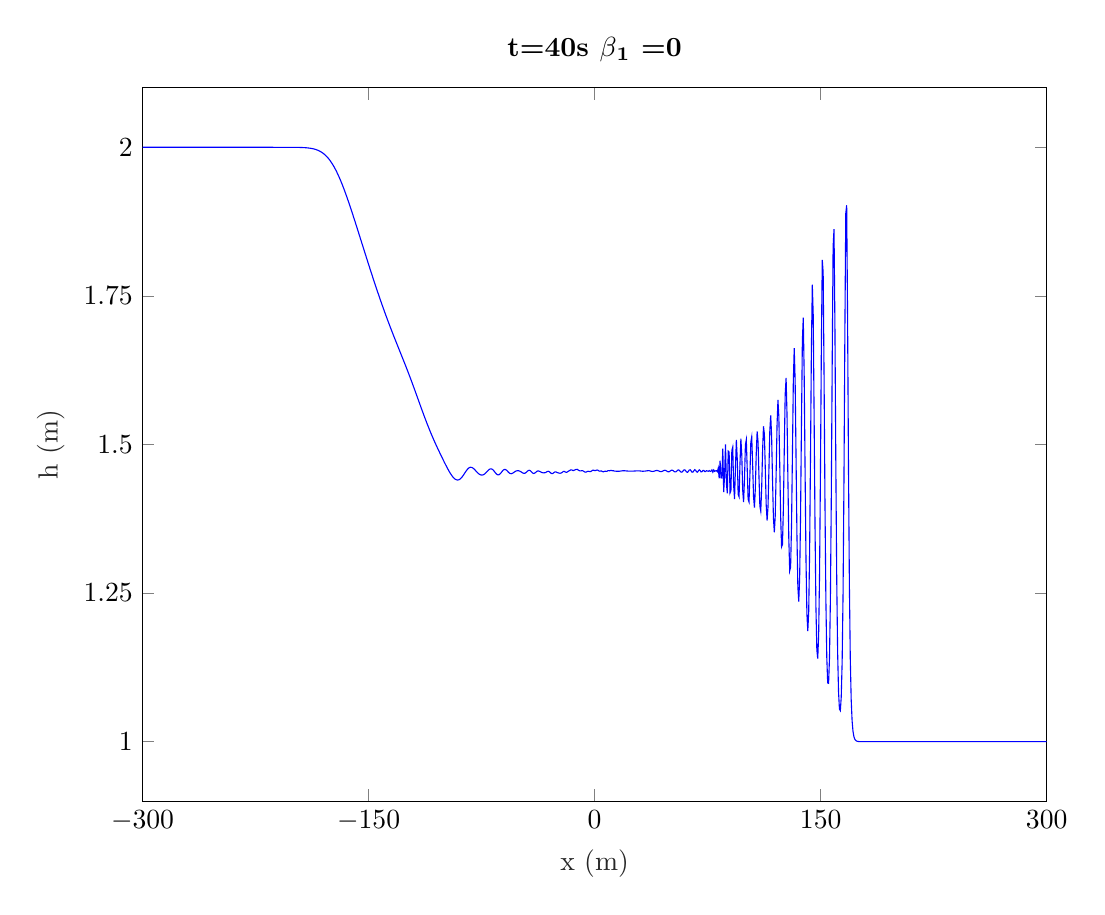
\begin{tikzpicture}

\begin{axis}[%
width=4.521in,
height=3.566in,
at={(0.758in,0.481in)},
scale only axis,
xmin=-300,
xmax=300,
xtick={-300, -150,    0,  150,  300},
xlabel style={font=\color{white!15!black}},
xlabel={x (m)},
ymin=0.9,
ymax=2.1,
ytick={   1, 1.25,  1.5, 1.75,    2},
ylabel style={font=\color{white!15!black}},
ylabel={h (m)},
axis background/.style={fill=white},
title style={font=\bfseries},
title={$\text{t=40s   }\beta{}_\text{1}\text{ =0}$}
]
\addplot [color=blue, forget plot]
  table[row sep=crcr]{%
-300.18000900045	2\\
-299.57997899895	2\\
-298.97994899745	2\\
-298.37991899595	2\\
-297.77988899445	2\\
-297.17985899295	2\\
-296.57982899145	2\\
-295.979798989949	2\\
-295.379768988449	2\\
-294.779738986949	2\\
-294.179708985449	2\\
-293.579678983949	2\\
-292.979648982449	2\\
-292.379618980949	2\\
-291.779588979449	2\\
-291.179558977949	2\\
-290.579528976449	2\\
-289.979498974949	2\\
-289.379468973449	2\\
-288.779438971949	2\\
-288.179408970449	2\\
-287.579378968948	2\\
-286.979348967448	2\\
-286.379318965948	2\\
-285.779288964448	2\\
-285.179258962948	2\\
-284.579228961448	2\\
-283.979198959948	2\\
-283.379168958448	2\\
-282.779138956948	2\\
-282.179108955448	2\\
-281.579078953948	2\\
-280.979048952448	2\\
-280.379018950948	2\\
-279.778988949447	2\\
-279.178958947947	2\\
-278.578928946447	2\\
-277.978898944947	2\\
-277.378868943447	2\\
-276.778838941947	2\\
-276.178808940447	2\\
-275.578778938947	2\\
-274.978748937447	2\\
-274.378718935947	2\\
-273.778688934447	2\\
-273.178658932947	2\\
-272.578628931447	2\\
-271.978598929946	2\\
-271.378568928446	2\\
-270.778538926946	2\\
-270.178508925446	2\\
-269.578478923946	2\\
-268.978448922446	2\\
-268.378418920946	2\\
-267.778388919446	2\\
-267.178358917946	2\\
-266.578328916446	2\\
-265.978298914946	2\\
-265.378268913446	2\\
-264.778238911946	2\\
-264.178208910446	2\\
-263.578178908945	2\\
-262.978148907445	2\\
-262.378118905945	2\\
-261.778088904445	2\\
-261.178058902945	2\\
-260.578028901445	2\\
-259.977998899945	2\\
-259.377968898445	2\\
-258.777938896945	2\\
-258.177908895445	2\\
-257.577878893945	2\\
-256.977848892445	2\\
-256.377818890945	2\\
-255.777788889444	2\\
-255.177758887944	1.99999999999999\\
-254.577728886444	1.99999999999999\\
-253.977698884944	1.99999999999998\\
-253.377668883444	1.99999999999996\\
-252.777638881944	1.99999999999995\\
-252.177608880444	1.99999999999992\\
-251.577578878944	1.99999999999989\\
-250.977548877444	1.99999999999985\\
-250.377518875944	1.9999999999998\\
-249.777488874444	1.99999999999973\\
-249.177458872944	1.99999999999964\\
-248.577428871444	1.99999999999952\\
-247.977398869943	1.99999999999936\\
-247.377368868443	1.99999999999916\\
-246.777338866943	1.9999999999989\\
-246.177308865443	1.99999999999856\\
-245.577278863943	1.99999999999811\\
-244.977248862443	1.99999999999754\\
-244.377218860943	1.99999999999679\\
-243.777188859443	1.99999999999581\\
-243.177158857943	1.99999999999455\\
-242.577128856443	1.99999999999291\\
-241.977098854943	1.9999999999908\\
-241.377068853443	1.99999999998806\\
-240.777038851943	1.99999999998452\\
-240.177008850443	1.99999999997995\\
-239.576978848942	1.99999999997406\\
-238.976948847442	1.99999999996646\\
-238.376918845942	1.99999999995666\\
-237.776888844442	1.99999999994407\\
-237.176858842942	1.99999999992787\\
-236.576828841442	1.99999999990706\\
-235.976798839942	1.99999999988034\\
-235.376768838442	1.99999999984608\\
-234.776738836942	1.99999999980218\\
-234.176708835442	1.99999999974598\\
-233.576678833942	1.9999999996741\\
-232.976648832442	1.99999999958224\\
-232.376618830942	1.99999999946496\\
-231.776588829441	1.99999999931537\\
-231.176558827941	1.99999999912475\\
-230.576528826441	1.99999999888206\\
-229.976498824941	1.99999999857339\\
-229.376468823441	1.99999999818116\\
-228.776438821941	1.99999999768325\\
-228.176408820441	1.99999999705181\\
-227.576378818941	1.99999999625181\\
-226.976348817441	1.99999999523928\\
-226.376318815941	1.99999999395907\\
-225.776288814441	1.99999999234204\\
-225.176258812941	1.99999999030172\\
-224.576228811441	1.99999998772996\\
-223.976198809941	1.99999998449177\\
-223.37616880844	1.99999998041881\\
-222.77613880694	1.99999997530139\\
-222.17610880544	1.99999996887869\\
-221.57607880394	1.99999996082665\\
-220.97604880244	1.99999995074316\\
-220.37601880094	1.9999999381299\\
-219.77598879944	1.99999992237016\\
-219.17595879794	1.99999990270167\\
-218.57592879644	1.99999987818353\\
-217.97589879494	1.99999984765594\\
-217.37586879344	1.99999980969121\\
-216.77583879194	1.99999976253436\\
-216.17580879044	1.99999970403118\\
-215.575778788939	1.99999963154112\\
-214.975748787439	1.99999954183236\\
-214.375718785939	1.99999943095516\\
-213.775688784439	1.99999929408975\\
-213.175658782939	1.99999912536366\\
-212.575628781439	1.99999891763294\\
-211.975598779939	1.99999866222065\\
-211.375568778439	1.99999834860488\\
-210.775538776939	1.99999796404735\\
-210.175508775439	1.9999974931523\\
-209.575478773939	1.99999691734367\\
-208.975448772439	1.99999621424697\\
-208.375418770939	1.99999535696\\
-207.775388769438	1.99999431319487\\
-207.175358767938	1.99999304427071\\
-206.575328766438	1.99999150393456\\
-205.975298764938	1.99998963698459\\
-205.375268763438	1.99998737766711\\
-204.775238761938	1.99998464781544\\
-204.175208760438	1.99998135469575\\
-203.575178758938	1.99997738852122\\
-202.975148757438	1.99997261959298\\
-202.375118755938	1.99996689502274\\
-201.775088754438	1.99996003498926\\
-201.175058752938	1.99995182847814\\
-200.575028751438	1.99994202845247\\
-199.974998749937	1.99993034640063\\
-199.374968748437	1.99991644620762\\
-198.774938746937	1.99989993729735\\
-198.174908745437	1.99988036699644\\
-197.574878743937	1.99985721207524\\
-196.974848742437	1.99982986942932\\
-196.374818740937	1.99979764587527\\
-195.774788739437	1.99975974704867\\
-195.174758737937	1.99971526540993\\
-194.574728736437	1.99966316738584\\
-193.974698734937	1.99960227970126\\
-193.374668733437	1.99953127498743\\
-192.774638731937	1.99944865678961\\
-192.174608730437	1.99935274413907\\
-191.574578728936	1.99924165590065\\
-190.974548727436	1.99911329515811\\
-190.374518725936	1.99896533395366\\
-189.774488724436	1.99879519875446\\
-189.174458722936	1.99860005707531\\
-188.574428721436	1.99837680574223\\
-187.974398719936	1.99812206133171\\
-187.374368718436	1.99783215336384\\
-186.774338716936	1.99750312085964\\
-186.174308715436	1.99713071289017\\
-185.574278713936	1.99671039374398\\
-184.974248712436	1.99623735331542\\
-184.374218710936	1.99570652326662\\
-183.774188709435	1.99511259943686\\
-183.174158707935	1.99445007086287\\
-182.574128706435	1.9937132556319\\
-181.974098704935	1.99289634361602\\
-181.374068703435	1.99199344593549\\
-180.774038701935	1.99099865077358\\
-180.174008700435	1.98990608492497\\
-179.573978698935	1.98870998021081\\
-178.973948697435	1.98740474364917\\
-178.373918695935	1.98598503004052\\
-177.773888694435	1.98444581542858\\
-177.173858692935	1.98278246973891\\
-176.573828691435	1.9809908267947\\
-175.973798689934	1.97906724987009\\
-175.373768688434	1.97700869097437\\
-174.773738686934	1.97481274216857\\
-174.173708685434	1.97247767739873\\
-173.573678683934	1.97000248358291\\
-172.973648682434	1.96738688000144\\
-172.373618680934	1.96463132539891\\
-171.773588679434	1.96173701259513\\
-171.173558677934	1.95870585080162\\
-170.573528676434	1.95554043623058\\
-169.973498674934	1.95224401194557\\
-169.373468673434	1.94882041821958\\
-168.773438671934	1.94527403492341\\
-168.173408670434	1.94160971765389\\
-167.573378668933	1.93783272942237\\
-166.973348667433	1.93394866975806\\
-166.373318665933	1.92996340304039\\
-165.773288664433	1.92588298776829\\
-165.173258662933	1.92171360831131\\
-164.573228661433	1.91746151048076\\
-163.973198659933	1.91313294202215\\
-163.373168658433	1.90873409887715\\
-162.773138656933	1.90427107780662\\
-162.173108655433	1.89974983571822\\
-161.573078653933	1.8951761558117\\
-160.973048652433	1.89055562045077\\
-160.373018650933	1.88589359049549\\
-159.772988649432	1.88119519068876\\
-159.172958647932	1.87646530058296\\
-158.572928646432	1.87170855041856\\
-157.972898644932	1.86692932132265\\
-157.372868643432	1.8621317491783\\
-156.772838641932	1.85731973152122\\
-156.172808640432	1.85249693684427\\
-155.572778638932	1.84766681572867\\
-154.972748637432	1.84283261326833\\
-154.372718635932	1.83799738230778\\
-153.772688634432	1.83316399707085\\
-153.172658632932	1.82833516681368\\
-152.572628631432	1.82351344919043\\
-151.972598629931	1.81870126307047\\
-151.372568628431	1.81390090059177\\
-150.772538626931	1.80911453827535\\
-150.172508625431	1.80434424706004\\
-149.572478623931	1.79959200114521\\
-148.972448622431	1.79485968555224\\
-148.372418620931	1.79014910233305\\
-147.772388619431	1.78546197536776\\
-147.172358617931	1.78079995370285\\
-146.572328616431	1.77616461338817\\
-145.972298614931	1.77155745777559\\
-145.372268613431	1.76697991624593\\
-144.772238611931	1.76243334133363\\
-144.172208610431	1.75791900422339\\
-143.57217860893	1.7534380885981\\
-142.97214860743	1.74899168282692\\
-142.37211860593	1.74458077049412\\
-141.77208860443	1.74020621928733\\
-141.17205860293	1.73586876828683\\
-140.57202860143	1.73156901372802\\
-139.97199859993	1.72730739334729\\
-139.37196859843	1.72308416946797\\
-138.77193859693	1.71889941103905\\
-138.17190859543	1.71475297490395\\
-137.57187859393	1.71064448665077\\
-136.97184859243	1.70657332147697\\
-136.37181859093	1.70253858559006\\
-135.771788589429	1.69853909875793\\
-135.171758587929	1.69457337871532\\
-134.571728586429	1.69063962822155\\
-133.971698584929	1.68673572564377\\
-133.371668583429	1.6828592200022\\
-132.771638581929	1.67900733145249\\
-132.171608580429	1.67517695818585\\
-131.571578578929	1.67136469069274\\
-130.971548577429	1.66756683425139\\
-130.371518575929	1.66377944036219\\
-129.771488574429	1.65999834764784\\
-129.171458572929	1.65621923247476\\
-128.571428571429	1.65243766922634\\
-127.971398569929	1.64864919977968\\
-127.371368568428	1.64484941131602\\
-126.771338566928	1.64103402114973\\
-126.171308565428	1.63719896681263\\
-125.571278563928	1.63334049920741\\
-124.971248562428	1.62945527627463\\
-124.371218560928	1.62554045433081\\
-123.771188559428	1.62159377405953\\
-123.171158557928	1.61761363809298\\
-122.571128556428	1.613599177224\\
-121.971098554928	1.60955030254192\\
-121.371068553428	1.60546774118235\\
-120.771038551928	1.60135305390385\\
-120.171008550428	1.59720863332254\\
-119.570978548927	1.59303768231356\\
-118.970948547427	1.58884417278094\\
-118.370918545927	1.58463278566376\\
-117.770888544427	1.58040883364264\\
-117.170858542927	1.57617816850598\\
-116.570828541427	1.57194707550425\\
-115.970798539927	1.5677221572542\\
-115.370768538427	1.56351020985526\\
-114.770738536927	1.55931809386395\\
-114.170708535427	1.55515260266753\\
-113.570678533927	1.55102033063997\\
-112.970648532427	1.54692754329524\\
-112.370618530927	1.5428800515156\\
-111.770588529426	1.53888309186762\\
-111.170558527926	1.53494121505636\\
-110.570528526426	1.53105818473205\\
-109.970498524926	1.52723688915955\\
-109.370468523426	1.52347926867854\\
-108.770438521926	1.51978626239214\\
-108.170408520426	1.51615777807119\\
-107.570378518926	1.51259268977967\\
-106.970348517426	1.50908886812086\\
-106.370318515926	1.50564324816989\\
-105.770288514426	1.50225193998352\\
-105.170258512926	1.49891038595619\\
-104.570228511426	1.49561356813673\\
-103.970198509925	1.49235626688112\\
-103.370168508425	1.48913336989989\\
-102.770138506925	1.4859402279331\\
-102.170108505425	1.48277305010037\\
-101.570078503925	1.47962932864415\\
-100.970048502425	1.47650827958474\\
-100.370018500925	1.47341128302775\\
-99.769988499425	1.47034230478074\\
-99.1699584979249	1.46730827973799\\
-98.5699284964248	1.46431943724776\\
-97.9698984949247	1.46138954928185\\
-97.3698684934247	1.45853608339678\\
-96.7698384919246	1.4557802437523\\
-96.1698084904245	1.45314688426826\\
-95.5697784889244	1.45066427776417\\
-94.9697484874244	1.44836372316073\\
-94.3697184859243	1.44627896932792\\
-93.7696884844242	1.44444542920449\\
-93.1696584829241	1.44289915232814\\
-92.5696284814241	1.44167551972235\\
-91.969598479924	1.44080762505926\\
-91.3695684784239	1.44032431415293\\
-90.7695384769239	1.44024787916678\\
-90.1695084754238	1.44059142656223\\
-89.5694784739237	1.44135603658063\\
-88.9694484724236	1.44252788714398\\
-88.3694184709235	1.44407561800733\\
-87.7693884694235	1.44594835679586\\
-87.1693584679234	1.44807488824499\\
-86.5693284664233	1.45036450205598\\
-85.9692984649232	1.45270997769468\\
-85.3692684634232	1.4549929691096\\
-84.7692384619231	1.45709169968322\\
-84.169208460423	1.45889041983931\\
-83.5691784589229	1.46028960165267\\
-82.9691484574229	1.4612154809713\\
-82.3691184559228	1.46162744779035\\
-81.7690884544227	1.46152200359639\\
-81.1690584529227	1.46093261425926\\
-80.5690284514226	1.45992541318729\\
-79.9689984499225	1.45859167836259\\
-79.3689684484224	1.45703838963898\\
-78.7689384469223	1.45537849118554\\
-78.1689084454223	1.45372230445572\\
-77.5688784439222	1.4521710795304\\
-76.9688484424221	1.45081304191328\\
-76.368818440922	1.44972167270454\\
-75.768788439422	1.44895544209002\\
-75.1687584379219	1.44855790057969\\
-74.5687284364218	1.4485570328096\\
-73.9686984349217	1.44896298005383\\
-73.3686684334217	1.44976387215092\\
-72.7686384319216	1.45092016854752\\
-72.1686084304215	1.45235888925573\\
-71.5685784289215	1.45396993909868\\
-70.9685484274214	1.45560723613624\\
-70.3685184259213	1.45709721728551\\
-69.7684884244212	1.45825619763259\\
-69.1684584229211	1.45891595359541\\
-68.5684284214211	1.45895411800534\\
-67.968398419921	1.45832339399709\\
-67.3683684184209	1.45707211536312\\
-66.7683384169208	1.45534955007664\\
-66.1683084154208	1.45339219238838\\
-65.5682784139207	1.45149160461266\\
-64.9682484124206	1.44994859580139\\
-64.3682184109205	1.44902145473694\\
-63.7681884094205	1.44887718236806\\
-63.1681584079204	1.44955450302272\\
-62.5681284064203	1.45094669689663\\
-61.9680984049203	1.45281039516857\\
-61.3680684034202	1.45480332800508\\
-60.7680384019201	1.456548185609\\
-60.16800840042	1.45771177464594\\
-59.5679783989199	1.45808072344393\\
-58.9679483974199	1.45761399425119\\
-58.3679183959198	1.45644971430356\\
-57.7678883944197	1.45487100739656\\
-57.1678583929196	1.45323200586173\\
-56.5678283914196	1.4518711826533\\
-55.9677983899195	1.45103479836398\\
-55.3677683884194	1.45083031175939\\
-54.7677383869193	1.45121892585099\\
-54.1677083854193	1.45204567432982\\
-53.5676783839192	1.45309369615527\\
-52.9676483824191	1.45414471558893\\
-52.3676183809191	1.45502571875682\\
-51.767588379419	1.45562917293804\\
-51.1675583779189	1.45590621300382\\
-50.5675283764188	1.45584505513061\\
-49.9674983749187	1.45545357390751\\
-49.3674683734187	1.45476087198652\\
-48.7674383719186	1.4538391063098\\
-48.1674083704185	1.45283000663002\\
-47.5673783689184	1.45195063158686\\
-46.9673483674184	1.45145712099511\\
-46.3673183659183	1.45156417828814\\
-45.7672883644182	1.45234407422255\\
-45.1672583629181	1.45365012884936\\
-44.5672283614181	1.45511337556744\\
-43.967198359918	1.45624023330711\\
-43.3671683584179	1.45659379921237\\
-42.7671383569178	1.45599052724304\\
-42.1671083554178	1.45461139695685\\
-41.5670783539177	1.45296068765736\\
-40.9670483524176	1.45166801804579\\
-40.3670183509175	1.45122090941498\\
-39.7669883494175	1.45174955261362\\
-39.1669583479174	1.45297623605091\\
-38.5669283464173	1.45434925783493\\
-37.9668983449172	1.45531014855034\\
-37.3668683434172	1.45554899595544\\
-36.7668383419171	1.45511055230534\\
-36.166808340417	1.45429982716881\\
-35.5667783389169	1.45346726726486\\
-34.9667483374168	1.4528281802814\\
-34.3667183359168	1.45243178788984\\
-33.7666883344167	1.45226779065174\\
-33.1666583329167	1.45238128838186\\
-32.5666283314166	1.45285847934045\\
-31.9665983299165	1.45366963458597\\
-31.3665683284164	1.45451764836471\\
-30.7665383269164	1.45489307914899\\
-30.1665083254163	1.45439391574771\\
-29.5664783239162	1.45309715591883\\
-28.9664483224161	1.45164958791444\\
-28.3664183209161	1.45089479261434\\
-27.766388319416	1.45126820941499\\
-27.1663583179159	1.45244384893406\\
-26.5663283164158	1.45357073730277\\
-25.9662983149157	1.4539413797891\\
-25.3662683134157	1.45350748897237\\
-24.7662383119156	1.45276163122664\\
-24.1662083104155	1.45216889463627\\
-23.5661783089154	1.45180698266623\\
-22.9661483074154	1.45160297406358\\
-22.3661183059153	1.45174589018239\\
-21.7660883044152	1.45255816842402\\
-21.1660583029151	1.45385566120655\\
-20.5660283014151	1.45475016545474\\
-19.965998299915	1.45450875854412\\
-19.3659682984149	1.45355126126331\\
-18.7659382969148	1.45309004352285\\
-18.1659082954148	1.45367784215267\\
-17.5658782939147	1.45472342086542\\
-16.9658482924146	1.45564632417132\\
-16.3658182909145	1.45658397464143\\
-15.7657882894144	1.45736215319329\\
-15.1657582879144	1.45716079023485\\
-14.5657282864143	1.45626001442094\\
-13.9656982849143	1.45614966497008\\
-13.3656682834142	1.45690374434387\\
-12.7656382819141	1.45749891444603\\
-12.165608280414	1.4581344422249\\
-11.565578278914	1.45822616692518\\
-10.9655482774139	1.4571087997303\\
-10.3655182759138	1.45618060733565\\
-9.76548827441371	1.45547283048476\\
-9.16545827291367	1.45559894417673\\
-8.56542827141357	1.45593075943644\\
-7.96539826991352	1.4558817167353\\
-7.36536826841342	1.45506937368376\\
-6.76533826691332	1.45401127293872\\
-6.16530826541327	1.45337321709096\\
-5.56527826391317	1.4536781342112\\
-4.96524826241313	1.45447274408421\\
-4.36521826091303	1.4548939812157\\
-3.76518825941298	1.454687703494\\
-3.16515825791288	1.454322701131\\
-2.56512825641283	1.45453900776814\\
-1.96509825491273	1.45553825150814\\
-1.36506825341269	1.45657372617656\\
-0.765038251912586	1.45676239852151\\
-0.165008250412541	1.45625255775326\\
0.435021751087561	1.45604702203302\\
1.03505175258761	1.45658117326326\\
1.63508175408771	1.45704726816473\\
2.23511175558775	1.45654161642296\\
2.83514175708785	1.45548258956212\\
3.43517175858796	1.45505581296102\\
4.035201760088	1.45537203208681\\
4.6352317615881	1.45528884871077\\
5.23526176308815	1.45442891687689\\
5.83529176458825	1.45400173965363\\
6.43532176608829	1.45462151284959\\
7.03535176758839	1.45508113173752\\
7.63538176908844	1.4547663394226\\
8.23541177058854	1.45497134376722\\
8.83544177208859	1.4558606738369\\
9.43547177358869	1.45591361794192\\
10.0355017750887	1.45575629335578\\
10.6355317765888	1.45642778204639\\
11.2355617780889	1.4562096361537\\
11.835591779589	1.45581768192572\\
12.435621781089	1.45590914785505\\
13.0356517825891	1.45524955346321\\
13.6356817840892	1.45526826811137\\
14.2357117855893	1.45497088604472\\
14.8357417870894	1.45491840820245\\
15.4357717885894	1.4548744064924\\
16.0358017900895	1.45489605423915\\
16.6358317915896	1.45505317401213\\
17.2358617930897	1.45523006348184\\
17.8358917945897	1.45552109320442\\
18.4359217960898	1.45570693124438\\
19.0359517975899	1.45582498724267\\
19.63598179909	1.4558248003974\\
20.23601180059	1.45567189621334\\
20.8360418020901	1.45551094870365\\
21.4360718035902	1.45538873524722\\
22.0361018050903	1.45527199169531\\
22.6361318065904	1.45521148876119\\
23.2361618080904	1.45523413195696\\
23.8361918095905	1.45525210432366\\
24.4362218110905	1.45520853262384\\
25.0362518125906	1.45517130974564\\
25.6362818140907	1.45521742030735\\
26.2363118155908	1.45531979264802\\
26.8363418170908	1.45541313996499\\
27.4363718185909	1.45549247826943\\
28.036401820091	1.45558913663402\\
28.6364318215911	1.45568075183988\\
29.2364618230911	1.45568485691244\\
29.8364918245912	1.4555501671336\\
30.4365218260913	1.45532352558996\\
31.0365518275914	1.45511326757577\\
31.6365818290914	1.45499957202054\\
32.2366118305915	1.45499304527242\\
32.8366418320916	1.45506849406556\\
33.4366718335917	1.45521359396604\\
34.0367018350918	1.45542827986415\\
34.6367318365918	1.45568142739714\\
35.2367618380919	1.45588146840512\\
35.836791839592	1.45590991093476\\
36.4368218410921	1.45570025700323\\
37.0368518425921	1.4553009193839\\
37.6368818440922	1.45487165630364\\
38.2369118455923	1.45461223790879\\
38.8369418470924	1.45466150624329\\
39.4369718485924	1.45502623849707\\
40.0370018500925	1.4555687434192\\
40.6370318515926	1.45605889671631\\
41.2370618530927	1.45626860998942\\
41.8370918545928	1.45607287668918\\
42.4371218560928	1.45552123076941\\
43.0371518575929	1.45483749612282\\
43.6371818590929	1.45434043593634\\
44.237211860593	1.45430083014839\\
44.8372418620931	1.45479321329633\\
45.4372718635932	1.45562124093936\\
46.0373018650932	1.4563769234066\\
46.6373318665933	1.45663425955087\\
47.2373618680934	1.45619549084738\\
47.8373918695935	1.45524486484575\\
48.4374218710935	1.45429623424575\\
49.0374518725936	1.45392276400123\\
49.6374818740937	1.45440313928777\\
50.2375118755938	1.45550335712903\\
50.8375418770938	1.45655541660674\\
51.4375718785939	1.45684875694053\\
52.037601880094	1.45611972098241\\
52.6376318815941	1.45480008251646\\
53.2376618830942	1.45379487034106\\
53.8376918845942	1.45387606967078\\
54.4377218860943	1.4550825408931\\
55.0377518875944	1.45658915041948\\
55.6377818890945	1.45723494292348\\
56.2378118905945	1.45642000981425\\
56.8378418920946	1.45467843793553\\
57.4378718935947	1.45338077665893\\
58.0379018950948	1.45366072711796\\
58.6379318965948	1.45539668203877\\
59.2379618980949	1.45715534809527\\
59.837991899595	1.45733756619258\\
60.4380219010951	1.45567570157232\\
61.0380519025952	1.45365581058527\\
61.6380819040952	1.45324058920192\\
62.2381119055953	1.45493262651613\\
62.8381419070953	1.45708420736981\\
63.4381719085955	1.45741089160969\\
64.0382019100955	1.45545792613299\\
64.6382319115956	1.45332800944642\\
65.2382619130956	1.45348593083477\\
65.8382919145957	1.45584123383908\\
66.4383219160958	1.45759322665719\\
67.0383519175959	1.45652355022682\\
67.6383819190959	1.45399878136141\\
68.238411920596	1.45340922723883\\
68.8384419220961	1.45557745876934\\
69.4384719235962	1.45737689127702\\
70.0385019250962	1.45613812228216\\
70.6385319265963	1.45386320656291\\
71.2385619280964	1.45415519164769\\
71.8385919295965	1.45624122546205\\
72.4386219310966	1.45630004086244\\
73.0386519325966	1.45449173271734\\
73.6386819340967	1.45447966388231\\
74.2387119355968	1.45579236540747\\
74.8387419370969	1.45531707786838\\
75.4387719385969	1.45497291719241\\
76.038801940097	1.45599181368554\\
76.6388319415971	1.45481802747273\\
77.2388619430972	1.45515717223788\\
77.8388919445972	1.457197113338\\
78.4389219460973	1.45343568513504\\
79.0389519475974	1.45713211871647\\
79.6389819490975	1.45475288629531\\
80.2390119505975	1.45569055216403\\
80.8390419520976	1.45583639051766\\
81.4390719535977	1.45412647065987\\
82.0391019550977	1.46029230338064\\
82.6391319565979	1.4431492903086\\
83.2391619580979	1.47284236402239\\
83.839191959598	1.44397801137836\\
84.439221961098	1.44364769364167\\
85.0392519625981	1.49299493524277\\
85.6392819640982	1.41982603416809\\
86.2393119655983	1.44873324186947\\
86.8393419670983	1.50023224623582\\
87.4393719685984	1.43408728826743\\
88.0394019700985	1.41788829736551\\
88.6394319715986	1.48869963166548\\
89.2394619730986	1.48716631437834\\
89.8394919745987	1.4182864693163\\
90.4395219760988	1.42214811908947\\
91.0395519775989	1.48971156876621\\
91.639581979099	1.49554156159226\\
92.239611980599	1.43104916331449\\
92.8396419820991	1.40812917776769\\
93.4396719835992	1.46120939325429\\
94.0397019850993	1.5077125787574\\
94.6397319865993	1.47555393539044\\
95.2397619880994	1.41586925171461\\
95.8397919895995	1.41198906439279\\
96.4398219910996	1.46744099396161\\
97.0398519925996	1.50974583268082\\
97.6398819940997	1.48259176812512\\
98.2399119955998	1.42313255473307\\
98.8399419970999	1.40292636689158\\
99.4399719985999	1.44287410576888\\
100.0400020001	1.4992685356187\\
100.6400320016	1.50792635859739\\
101.2400620031	1.45940361702062\\
101.8400920046	1.40783838299693\\
102.4401220061	1.40338331555444\\
103.0401520076	1.44944996384013\\
103.6401820091	1.50372038834835\\
104.240212010601	1.51266357613091\\
104.840242012101	1.467419106357\\
105.440272013601	1.41206454619875\\
106.040302015101	1.39360692348689\\
106.640332016601	1.42598042557453\\
107.240362018101	1.48488372597059\\
107.840392019601	1.52197384273132\\
108.440422021101	1.50395444588372\\
109.040452022601	1.44669006337406\\
109.640482024101	1.39635475818116\\
110.240512025601	1.38782500621854\\
110.840542027101	1.4268255693297\\
111.440572028601	1.48923753852192\\
112.040602030102	1.5305784502991\\
112.640632031602	1.51740208047127\\
113.240662033102	1.45940762887223\\
113.840692034602	1.398481003838\\
114.440722036102	1.37212301556592\\
115.040752037602	1.39485626986978\\
115.640782039102	1.45661116756165\\
116.240812040602	1.52298562573444\\
116.840842042102	1.54892030111907\\
117.440872043602	1.51351975139791\\
118.040902045102	1.44104207956469\\
118.640932046602	1.37625997480477\\
119.240962048102	1.35203811057422\\
119.840992049603	1.37995386062675\\
120.441022051103	1.45099607697641\\
121.041052052603	1.53247869703535\\
121.641082054103	1.57479734643644\\
122.241112055603	1.54630750004125\\
122.841142057103	1.46454876621274\\
123.441172058603	1.37820625267925\\
124.041202060103	1.32772632902228\\
124.641232061603	1.33186910657072\\
125.241262063103	1.39223875726795\\
125.841292064603	1.49132851481535\\
126.441322066103	1.58405800466284\\
127.041352067603	1.61185274697386\\
127.641382069103	1.55197321952518\\
128.241412070604	1.44234344349773\\
128.841442072104	1.34162817734399\\
129.441472073604	1.28739035853258\\
130.041502075104	1.29377073480397\\
130.641532076604	1.36271248421741\\
131.241562078104	1.48134185345581\\
131.841592079604	1.60534910755018\\
132.441622081104	1.66218520442224\\
133.041652082604	1.6087088742523\\
133.641682084104	1.47965878772615\\
134.241712085604	1.34766940660142\\
134.841742087104	1.26092404237149\\
135.441772088604	1.2354842364763\\
136.041802090105	1.27529600102321\\
136.641832091605	1.38052180965429\\
137.241862093105	1.53373335989308\\
137.841892094605	1.67429572778056\\
138.441922096105	1.71343848687986\\
139.041952097605	1.61919192592726\\
139.641982099105	1.45591114878683\\
140.242012100605	1.30789431667099\\
140.842042102105	1.2157764686597\\
141.442072103605	1.18600133408475\\
142.042102105105	1.2184336023481\\
142.642132106605	1.31731657693884\\
143.242162108105	1.47978063022023\\
143.842192109605	1.66312042342639\\
144.442222111106	1.76897963645694\\
145.042252112606	1.71799573988705\\
145.642282114106	1.54731478421325\\
146.242312115606	1.36158976712912\\
146.842342117106	1.22673092819569\\
147.442372118606	1.15496405572278\\
148.042402120106	1.13961525118315\\
148.642432121606	1.17889037302779\\
149.242462123106	1.2811119641618\\
149.842492124606	1.45262494953909\\
150.442522126106	1.66258556147734\\
151.042552127606	1.81071768961978\\
151.642582129106	1.78933600239176\\
152.242612130607	1.61414718101299\\
152.842642132107	1.40239926785751\\
153.442672133607	1.23932433432052\\
154.042702135107	1.14214686507064\\
154.642732136607	1.09875338274114\\
155.242762138107	1.09816832517072\\
155.842792139607	1.14093678148346\\
156.442822141107	1.23973432745796\\
157.042852142607	1.40991041324357\\
157.642882144107	1.63743631485035\\
158.242912145607	1.83266016983896\\
158.842942147107	1.86216687455905\\
159.442972148607	1.70097590154969\\
160.043002150107	1.46760105400817\\
160.643032151608	1.27382605059895\\
161.243062153108	1.15047814687047\\
161.843092154608	1.08384633766137\\
162.443122156108	1.05475461790132\\
163.043152157608	1.05221257402433\\
163.643182159108	1.07547633755314\\
164.243212160608	1.13435216840856\\
164.843242162108	1.24857662304813\\
165.443272163608	1.43788921304747\\
166.043302165108	1.68577836745525\\
166.643332166608	1.8888260752961\\
167.243362168108	1.90243603382437\\
167.843392169608	1.7148333345937\\
168.443422171109	1.46404500287145\\
169.043452172609	1.26416527238824\\
169.643482174109	1.13940219325407\\
170.243512175609	1.07065374752166\\
170.843542177109	1.03508137601413\\
171.443572178609	1.01724180321419\\
172.043602180109	1.00843169157527\\
172.643632181609	1.00411331716987\\
173.243662183109	1.00200430898851\\
173.843692184609	1.00097611463626\\
174.443722186109	1.00047526061258\\
175.043752187609	1.0002313778165\\
175.643782189109	1.00011264238614\\
176.24381219061	1.00005483875581\\
176.84384219211	1.0000266984849\\
177.44387219361	1.00001299878572\\
178.04390219511	1.00000632904432\\
178.64393219661	1.0000030817246\\
179.24396219811	1.00000150061945\\
179.84399219961	1.00000073075012\\
180.44402220111	1.00000035586823\\
181.04405220261	1.00000017331331\\
181.64408220411	1.00000008441067\\
182.24411220561	1.00000004111364\\
182.84414220711	1.00000002002617\\
183.44417220861	1.00000000975514\\
184.04420221011	1.00000000475219\\
184.644232211611	1.00000000231514\\
185.244262213111	1.00000000112794\\
185.844292214611	1.00000000054956\\
186.444322216111	1.00000000026778\\
187.044352217611	1.00000000013048\\
187.644382219111	1.00000000006358\\
188.244412220611	1.00000000003098\\
188.844442222111	1.0000000000151\\
189.444472223611	1.00000000000735\\
190.044502225111	1.00000000000358\\
190.644532226611	1.00000000000174\\
191.244562228111	1.00000000000085\\
191.844592229611	1.00000000000041\\
192.444622231112	1.0000000000002\\
193.044652232612	1.00000000000009\\
193.644682234112	1.00000000000004\\
194.244712235612	1.00000000000002\\
194.844742237112	1\\
195.444772238612	1\\
196.044802240112	1\\
196.644832241612	1\\
197.244862243112	1\\
197.844892244612	1\\
198.444922246112	1\\
199.044952247612	1\\
199.644982249112	1\\
200.245012250613	1\\
200.845042252113	1\\
201.445072253613	1\\
202.045102255113	1\\
202.645132256613	1\\
203.245162258113	1\\
203.845192259613	1\\
204.445222261113	1\\
205.045252262613	1\\
205.645282264113	1\\
206.245312265613	1\\
206.845342267113	1\\
207.445372268613	1\\
208.045402270114	1\\
208.645432271614	1\\
209.245462273114	1\\
209.845492274614	1\\
210.445522276114	1\\
211.045552277614	1\\
211.645582279114	1\\
212.245612280614	1\\
212.845642282114	1\\
213.445672283614	1\\
214.045702285114	1\\
214.645732286614	1\\
215.245762288114	1\\
215.845792289614	1\\
216.445822291115	1\\
217.045852292615	1\\
217.645882294115	1\\
218.245912295615	1\\
218.845942297115	1\\
219.445972298615	1\\
220.046002300115	1\\
220.646032301615	1\\
221.246062303115	1\\
221.846092304615	1\\
222.446122306115	1\\
223.046152307615	1\\
223.646182309115	1\\
224.246212310616	1\\
224.846242312116	1\\
225.446272313616	1\\
226.046302315116	1\\
226.646332316616	1\\
227.246362318116	1\\
227.846392319616	1\\
228.446422321116	1\\
229.046452322616	1\\
229.646482324116	1\\
230.246512325616	1\\
230.846542327116	1\\
231.446572328616	1\\
232.046602330116	1\\
232.646632331617	1\\
233.246662333117	1\\
233.846692334617	1\\
234.446722336117	1\\
235.046752337617	1\\
235.646782339117	1\\
236.246812340617	1\\
236.846842342117	1\\
237.446872343617	1\\
238.046902345117	1\\
238.646932346617	1\\
239.246962348117	1\\
239.846992349617	1\\
240.447022351118	1\\
241.047052352618	1\\
241.647082354118	1\\
242.247112355618	1\\
242.847142357118	1\\
243.447172358618	1\\
244.047202360118	1\\
244.647232361618	1\\
245.247262363118	1\\
245.847292364618	1\\
246.447322366118	1\\
247.047352367618	1\\
247.647382369118	1\\
248.247412370619	1\\
248.847442372119	1\\
249.447472373619	1\\
250.047502375119	1\\
250.647532376619	1\\
251.247562378119	1\\
251.847592379619	1\\
252.447622381119	1\\
253.047652382619	1\\
253.647682384119	1\\
254.247712385619	1\\
254.847742387119	1\\
255.447772388619	1\\
256.04780239012	1\\
256.64783239162	1\\
257.24786239312	1\\
257.84789239462	1\\
258.44792239612	1\\
259.04795239762	1\\
259.64798239912	1\\
260.24801240062	1\\
260.84804240212	1\\
261.44807240362	1\\
262.04810240512	1\\
262.64813240662	1\\
263.24816240812	1\\
263.84819240962	1\\
264.448222411121	1\\
265.048252412621	1\\
265.648282414121	1\\
266.248312415621	1\\
266.848342417121	1\\
267.448372418621	1\\
268.048402420121	1\\
268.648432421621	1\\
269.248462423121	1\\
269.848492424621	1\\
270.448522426121	1\\
271.048552427621	1\\
271.648582429121	1\\
272.248612430622	1\\
272.848642432122	1\\
273.448672433622	1\\
274.048702435122	1\\
274.648732436622	1\\
275.248762438122	1\\
275.848792439622	1\\
276.448822441122	1\\
277.048852442622	1\\
277.648882444122	1\\
278.248912445622	1\\
278.848942447122	1\\
279.448972448622	1\\
280.049002450123	1\\
280.649032451623	1\\
281.249062453123	1\\
281.849092454623	1\\
282.449122456123	1\\
283.049152457623	1\\
283.649182459123	1\\
284.249212460623	1\\
284.849242462123	1\\
285.449272463623	1\\
286.049302465123	1\\
286.649332466623	1\\
287.249362468123	1\\
287.849392469623	1\\
288.449422471124	1\\
289.049452472624	1\\
289.649482474124	1\\
290.249512475624	1\\
290.849542477124	1\\
291.449572478624	1\\
292.049602480124	1\\
292.649632481624	1\\
293.249662483124	1\\
293.849692484624	1\\
294.449722486124	1\\
295.049752487624	1\\
295.649782489125	1\\
296.249812490625	1\\
296.849842492125	1\\
297.449872493625	1\\
298.049902495125	1\\
298.649932496625	1\\
299.249962498125	1\\
299.849992499625	1\\
};
\end{axis}
\end{tikzpicture}%
		\caption{$t=40s$}
	\end{subfigure}
	\begin{subfigure}{0.49\textwidth}
		\centering
		% This file was created by matlab2tikz.
%
%The latest updates can be retrieved from
%  http://www.mathworks.com/matlabcentral/fileexchange/22022-matlab2tikz-matlab2tikz
%where you can also make suggestions and rate matlab2tikz.
%
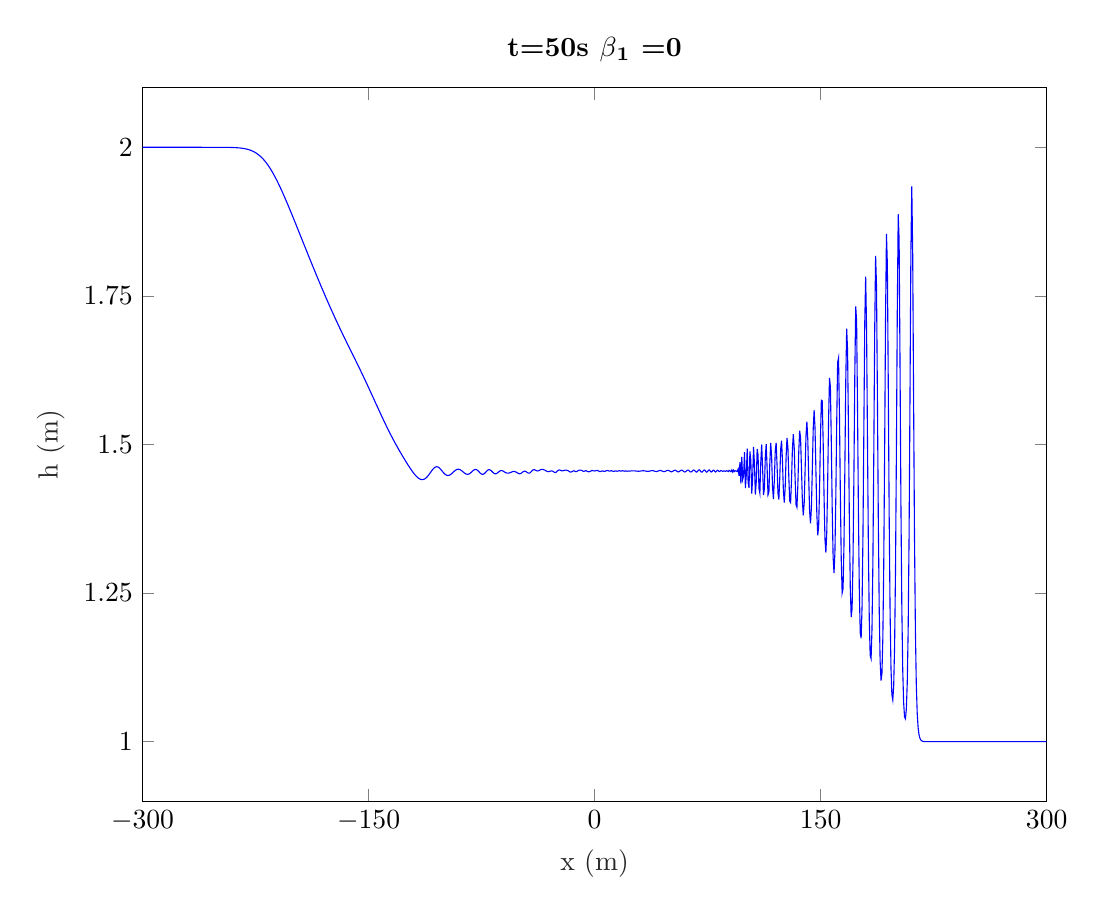
\begin{tikzpicture}

\begin{axis}[%
width=4.521in,
height=3.566in,
at={(0.758in,0.481in)},
scale only axis,
xmin=-300,
xmax=300,
xtick={-300, -150,    0,  150,  300},
xlabel style={font=\color{white!15!black}},
xlabel={x (m)},
ymin=0.9,
ymax=2.1,
ytick={   1, 1.25,  1.5, 1.75,    2},
ylabel style={font=\color{white!15!black}},
ylabel={h (m)},
axis background/.style={fill=white},
title style={font=\bfseries},
title={$\text{t=50s   }\beta{}_\text{1}\text{ =0}$}
]
\addplot [color=blue, forget plot]
  table[row sep=crcr]{%
-300.18000900045	2\\
-299.57997899895	1.99999999999933\\
-298.97994899745	1.99999999999927\\
-298.37991899595	1.99999999999916\\
-297.77988899445	1.999999999999\\
-297.17985899295	1.99999999999877\\
-296.57982899145	1.99999999999846\\
-295.979798989949	1.99999999999806\\
-295.379768988449	1.99999999999753\\
-294.779738986949	1.99999999999686\\
-294.179708985449	1.999999999996\\
-293.579678983949	1.9999999999949\\
-292.979648982449	1.9999999999935\\
-292.379618980949	1.99999999999172\\
-291.779588979449	1.99999999998946\\
-291.179558977949	1.99999999998659\\
-290.579528976449	1.99999999998295\\
-289.979498974949	1.99999999997835\\
-289.379468973449	1.99999999997252\\
-288.779438971949	1.99999999996515\\
-288.179408970449	1.99999999995583\\
-287.579378968948	1.99999999994407\\
-286.979348967448	1.99999999992924\\
-286.379318965948	1.99999999991053\\
-285.779288964448	1.99999999988698\\
-285.179258962948	1.99999999985732\\
-284.579228961448	1.99999999982002\\
-283.979198959948	1.99999999977316\\
-283.379168958448	1.99999999971431\\
-282.779138956948	1.99999999964048\\
-282.179108955448	1.99999999954792\\
-281.579078953948	1.99999999943199\\
-280.979048952448	1.99999999928689\\
-280.379018950948	1.99999999910546\\
-279.778988949447	1.99999999887877\\
-279.178958947947	1.99999999859579\\
-278.578928946447	1.99999999824284\\
-277.978898944947	1.99999999780299\\
-277.378868943447	1.99999999725535\\
-276.778838941947	1.99999999657408\\
-276.178808940447	1.99999999572735\\
-275.578778938947	1.99999999467591\\
-274.978748937447	1.99999999337144\\
-274.378718935947	1.99999999175456\\
-273.778688934447	1.99999998975227\\
-273.178658932947	1.99999998727503\\
-272.578628931447	1.99999998421306\\
-271.978598929946	1.99999998043192\\
-271.378568928446	1.99999997576716\\
-270.778538926946	1.99999997001786\\
-270.178508925446	1.99999996293879\\
-269.578478923946	1.99999995423094\\
-268.978448922446	1.99999994353022\\
-268.378418920946	1.99999993039374\\
-267.778388919446	1.99999991428341\\
-267.178358917946	1.99999989454622\\
-266.578328916446	1.99999987039067\\
-265.978298914946	1.99999984085855\\
-265.378268913446	1.99999980479121\\
-264.778238911946	1.99999976078943\\
-264.178208910446	1.99999970716552\\
-263.578178908945	1.99999964188647\\
-262.978148907445	1.99999956250644\\
-262.378118905945	1.99999946608679\\
-261.778088904445	1.99999934910142\\
-261.178058902945	1.99999920732508\\
-260.578028901445	1.99999903570158\\
-259.977998899945	1.99999882818878\\
-259.377968898445	1.99999857757648\\
-258.777938896945	1.99999827527285\\
-258.177908895445	1.99999791105458\\
-257.577878893945	1.99999747277487\\
-256.977848892445	1.99999694602326\\
-256.377818890945	1.99999631372969\\
-255.777788889444	1.99999555570494\\
-255.177758887944	1.99999464810829\\
-254.577728886444	1.99999356283217\\
-253.977698884944	1.99999226679258\\
-253.377668883444	1.9999907211127\\
-252.777638881944	1.99998888018594\\
-252.177608880444	1.99998669060331\\
-251.577578878944	1.99998408992872\\
-250.977548877444	1.99998100530422\\
-250.377518875944	1.99997735186632\\
-249.777488874444	1.99997303095269\\
-249.177458872944	1.99996792807798\\
-248.577428871444	1.99996191065593\\
-247.977398869943	1.99995482544468\\
-247.377368868443	1.99994649569137\\
-246.777338866943	1.99993671795245\\
-246.177308865443	1.99992525856607\\
-245.577278863943	1.99991184975462\\
-244.977248862443	1.99989618533674\\
-244.377218860943	1.99987791603131\\
-243.777188859443	1.99985664433922\\
-243.177158857943	1.99983191899399\\
-242.577128856443	1.99980322897843\\
-241.977098854943	1.99976999711197\\
-241.377068853443	1.99973157322324\\
-240.777038851943	1.99968722693264\\
-240.177008850443	1.99963614008342\\
-239.576978848942	1.99957739887365\\
-238.976948847442	1.99950998575867\\
-238.376918845942	1.99943277121136\\
-237.776888844442	1.99934450544798\\
-237.176858842942	1.99924381024804\\
-236.576828841442	1.99912917101943\\
-235.976798839942	1.99899892928197\\
-235.376768838442	1.99885127576591\\
-234.776738836942	1.99868424434227\\
-234.176708835442	1.9984957070227\\
-233.576678833942	1.99828337028207\\
-232.976648832442	1.99804477297029\\
-232.376618830942	1.99777728608644\\
-231.776588829441	1.9974781146891\\
-231.176558827941	1.99714430220877\\
-230.576528826441	1.99677273741196\\
-229.976498824941	1.99636016423923\\
-229.376468823441	1.99590319470162\\
-228.776438821941	1.99539832497044\\
-228.176408820441	1.99484195473449\\
-227.576378818941	1.99423040982679\\
-226.976348817441	1.99355996804134\\
-226.376318815941	1.9928268879705\\
-225.776288814441	1.9920274405981\\
-225.176258812941	1.99115794328506\\
-224.576228811441	1.99021479568725\\
-223.976198809941	1.98919451705266\\
-223.37616880844	1.98809378426199\\
-222.77613880694	1.98690946990689\\
-222.17610880544	1.98563867964833\\
-221.57607880394	1.9842787880666\\
-220.97604880244	1.98282747220845\\
-220.37601880094	1.98128274205648\\
-219.77598879944	1.97964296719336\\
-219.17595879794	1.97790689900703\\
-218.57592879644	1.9760736878821\\
-217.97589879494	1.97414289494307\\
-217.37586879344	1.97211449805302\\
-216.77583879194	1.96998889192185\\
-216.17580879044	1.96776688233409\\
-215.575778788939	1.96544967466259\\
-214.975748787439	1.96303885698342\\
-214.375718785939	1.9605363782439\\
-213.775688784439	1.95794452205426\\
-213.175658782939	1.95526587676902\\
-212.575628781439	1.95250330259539\\
-211.975598779939	1.94965989650888\\
-211.375568778439	1.94673895577234\\
-210.775538776939	1.94374394084396\\
-210.175508775439	1.94067843842469\\
-209.575478773939	1.9375461253388\\
-208.975448772439	1.93435073386812\\
-208.375418770939	1.93109601907291\\
-207.775388769438	1.92778572853755\\
-207.175358767938	1.92442357487909\\
-206.575328766438	1.92101321125738\\
-205.975298764938	1.9175582100294\\
-205.375268763438	1.91406204460095\\
-204.775238761938	1.91052807444871\\
-204.175208760438	1.90695953321592\\
-203.575178758938	1.90335951972704\\
-202.975148757438	1.89973099172101\\
-202.375118755938	1.89607676206871\\
-201.775088754438	1.8923994972175\\
-201.175058752938	1.88870171759343\\
-200.575028751438	1.8849857996884\\
-199.974998749937	1.88125397956396\\
-199.374968748437	1.87750835751401\\
-198.774938746937	1.87375090364469\\
-198.174908745437	1.86998346414839\\
-197.574878743937	1.86620776807063\\
-196.974848742437	1.86242543439141\\
-196.374818740937	1.85863797926522\\
-195.774788739437	1.85484682328739\\
-195.174758737937	1.85105329867515\\
-194.574728736437	1.84725865627289\\
-193.974698734937	1.84346407230895\\
-193.374668733437	1.83967065484786\\
-192.774638731937	1.83587944989686\\
-192.174608730437	1.83209144713725\\
-191.574578728936	1.82830758526212\\
-190.974548727436	1.82452875691035\\
-190.374518725936	1.8207558131937\\
-189.774488724436	1.816989567819\\
-189.174458722936	1.81323080081151\\
-188.574428721436	1.80948026184802\\
-187.974398719936	1.80573867321003\\
-187.374368718436	1.80200673236825\\
-186.774338716936	1.79828511420926\\
-186.174308715436	1.79457447291534\\
-185.574278713936	1.79087544350686\\
-184.974248712436	1.78718864305581\\
-184.374218710936	1.78351467157729\\
-183.774188709435	1.7798541126042\\
-183.174158707935	1.77620753344873\\
-182.574128706435	1.77257548515252\\
-181.974098704935	1.76895850212577\\
-181.374068703435	1.76535710147448\\
-180.774038701935	1.76177178201322\\
-180.174008700435	1.75820302296086\\
-179.573978698935	1.75465128231522\\
-178.973948697435	1.75111699490339\\
-178.373918695935	1.74760057010437\\
-177.773888694435	1.74410238924191\\
-177.173858692935	1.74062280264715\\
-176.573828691435	1.73716212639301\\
-175.973798689934	1.73372063870539\\
-175.373768688434	1.73029857606068\\
-174.773738686934	1.72689612898395\\
-174.173708685434	1.72351343756827\\
-173.573678683934	1.72015058674311\\
-172.973648682434	1.71680760132775\\
-172.373618680934	1.71348444091544\\
-171.773588679434	1.71018099464434\\
-171.173558677934	1.70689707592297\\
-170.573528676434	1.70363241719032\\
-169.973498674934	1.70038666480403\\
-169.373468673434	1.69715937416343\\
-168.773438671934	1.69395000518819\\
-168.173408670434	1.69075791828651\\
-167.573378668933	1.68758237095925\\
-166.973348667433	1.68442251519759\\
-166.373318665933	1.6812773958406\\
-165.773288664433	1.67814595006479\\
-165.173258662933	1.6750270081804\\
-164.573228661433	1.67191929590642\\
-163.973198659933	1.66882143828861\\
-163.373168658433	1.66573196541104\\
-162.773138656933	1.66264932003085\\
-162.173108655433	1.65957186723799\\
-161.573078653933	1.65649790620616\\
-160.973048652433	1.65342568405872\\
-160.373018650933	1.6503534118231\\
-159.772988649432	1.64727928239169\\
-159.172958647932	1.64420149034654\\
-158.572928646432	1.64111825344123\\
-157.972898644932	1.63802783546862\\
-157.372868643432	1.63492857018001\\
-156.772838641932	1.63181888586229\\
-156.172808640432	1.62869733012755\\
-155.572778638932	1.62556259442823\\
-154.972748637432	1.62241353778131\\
-154.372718635932	1.61924920917116\\
-153.772688634432	1.61606886810289\\
-153.172658632932	1.61287200279838\\
-152.572628631432	1.60965834556516\\
-151.972598629931	1.60642788492317\\
-151.372568628431	1.60318087414536\\
-150.772538626931	1.59991783595075\\
-150.172508625431	1.5966395631817\\
-149.572478623931	1.59334711539518\\
-148.972448622431	1.59004181139719\\
-148.372418620931	1.58672521784585\\
-147.772388619431	1.58339913413782\\
-147.172358617931	1.58006557387046\\
-146.572328616431	1.57672674323676\\
-145.972298614931	1.57338501675757\\
-145.372268613431	1.57004291078731\\
-144.772238611931	1.56670305524259\\
-144.172208610431	1.5633681640014\\
-143.57217860893	1.56004100440439\\
-142.97214860743	1.55672436626198\\
-142.37211860593	1.55342103073686\\
-141.77208860443	1.55013373943186\\
-141.17205860293	1.54686516397605\\
-140.57202860143	1.54361787636781\\
-139.97199859993	1.54039432030928\\
-139.37196859843	1.53719678375387\\
-138.77193859693	1.53402737289129\\
-138.17190859543	1.53088798781425\\
-137.57187859393	1.52778030014955\\
-136.97184859243	1.52470573299325\\
-136.37181859093	1.52166544356425\\
-135.771788589429	1.51866030908061\\
-135.171758587929	1.51569091646418\\
-134.571728586429	1.51275755658638\\
-133.971698584929	1.50986022387484\\
-133.371668583429	1.50699862219813\\
-132.771638581929	1.50417217802548\\
-132.171608580429	1.50138006190864\\
-131.571578578929	1.49862121934466\\
-130.971548577429	1.49589441203965\\
-130.371518575929	1.49319827049642\\
-129.771488574429	1.49053135868548\\
-129.171458572929	1.48789225132637\\
-128.571428571429	1.48527962400453\\
-127.971398569929	1.48269235598388\\
-127.371368568428	1.48012964515741\\
-126.771338566928	1.47759113412317\\
-126.171308565428	1.47507704590112\\
-125.571278563928	1.47258832733713\\
-124.971248562428	1.47012679779593\\
-124.371218560928	1.46769530033757\\
-123.771188559428	1.46529785220824\\
-123.171158557928	1.46293979114482\\
-122.571128556428	1.46062791366508\\
-121.971098554928	1.45837060113758\\
-121.371068553428	1.45617792892091\\
-120.771038551928	1.45406175312599\\
-120.171008550428	1.45203576846482\\
-119.570978548927	1.45011552906688\\
-118.970948547427	1.44831842193751\\
-118.370918545927	1.44666357979626\\
-117.770888544427	1.44517171632623\\
-117.170858542927	1.44386486246924\\
-116.570828541427	1.4427659775865\\
-115.970798539927	1.44189840463268\\
-115.370768538427	1.44128513492791\\
-114.770738536927	1.44094784714792\\
-114.170708535427	1.44090569047216\\
-113.570678533927	1.44117378484115\\
-112.970648532427	1.44176144842026\\
-112.370618530927	1.44267018953576\\
-111.770588529426	1.4438915410154\\
-111.170558527926	1.44540490370343\\
-110.570528526426	1.44717563106395\\
-109.970498524926	1.44915367061039\\
-109.370468523426	1.45127313948071\\
-108.770438521926	1.45345323013236\\
-108.170408520426	1.45560078921538\\
-107.570378518926	1.45761476466729\\
-106.970348517426	1.45939246707074\\
-106.370318515926	1.46083726490116\\
-105.770288514426	1.46186698485098\\
-105.170258512926	1.46242200530595\\
-104.570228511426	1.4624718992405\\
-103.970198509925	1.46201960605791\\
-103.370168508425	1.46110236953391\\
-102.770138506925	1.45978925161314\\
-102.170108505425	1.45817553748668\\
-101.570078503925	1.4563748082312\\
-100.970048502425	1.454509736871\\
-100.370018500925	1.45270272388448\\
-99.769988499425	1.45106728868007\\
-99.1699584979249	1.44970088776387\\
-98.5699284964248	1.44867948685474\\
-97.9698984949247	1.44805394836106\\
-97.3698684934247	1.4478482075521\\
-96.7698384919246	1.44805857125963\\
-96.1698084904245	1.44865540566194\\
-95.5697784889244	1.44958473581128\\
-94.9697484874244	1.4507720494152\\
-94.3697184859243	1.45212684575024\\
-93.7696884844242	1.45354831107673\\
-93.1696584829241	1.45493186600135\\
-92.5696284814241	1.45617625343213\\
-91.969598479924	1.45719070687413\\
-91.3695684784239	1.45790164515722\\
-90.7695384769239	1.45825831645052\\
-90.1695084754238	1.45823688686965\\
-89.5694784739237	1.45784264949804\\
-88.9694484724236	1.45711013483653\\
-88.3694184709235	1.45610120432352\\
-87.7693884694235	1.45490124119773\\
-87.1693584679234	1.45361366394351\\
-86.5693284664233	1.45235297539273\\
-85.9692984649232	1.45123653543074\\
-85.3692684634232	1.45037524178515\\
-84.7692384619231	1.44986337329515\\
-84.169208460423	1.44976804806574\\
-83.5691784589229	1.45011903822142\\
-82.9691484574229	1.45090023798606\\
-82.3691184559228	1.45204440606079\\
-81.7690884544227	1.45343327022704\\
-81.1690584529227	1.45490494497103\\
-80.5690284514226	1.45626988399142\\
-79.9689984499225	1.45733503537841\\
-79.3689684484224	1.45793364307061\\
-78.7689384469223	1.45795580099187\\
-78.1689084454223	1.45737337653485\\
-77.5688784439222	1.45625285020041\\
-76.9688484424221	1.45475182047711\\
-76.368818440922	1.45309827260996\\
-75.768788439422	1.45155559856266\\
-75.1687584379219	1.45037931011052\\
-74.5687284364218	1.44977280321465\\
-73.9686984349217	1.44984953378698\\
-73.3686684334217	1.45060800323237\\
-72.7686384319216	1.45192490055481\\
-72.1686084304215	1.45356970507566\\
-71.5685784289215	1.45524146453709\\
-70.9685484274214	1.45662392703211\\
-70.3685184259213	1.45744968625205\\
-69.7684884244212	1.45755915922041\\
-69.1684584229211	1.45693889278721\\
-68.5684284214211	1.45572737330943\\
-67.968398419921	1.45418535563752\\
-67.3683684184209	1.4526376746628\\
-66.7683384169208	1.45140123412865\\
-66.1683084154208	1.45071655207994\\
-65.5682784139207	1.45069807841059\\
-64.9682484124206	1.45131327909439\\
-64.3682184109205	1.4523943663717\\
-63.7681884094205	1.45367990083195\\
-63.1681584079204	1.45487719782378\\
-62.5681284064203	1.45573090661749\\
-61.9680984049203	1.45608039700457\\
-61.3680684034202	1.45589037460064\\
-60.7680384019201	1.45524828968577\\
-60.16800840042	1.45432988244583\\
-59.5679783989199	1.45334754220704\\
-58.9679483974199	1.45249736414622\\
-58.3679183959198	1.45192004188684\\
-57.7678883944197	1.45168321050941\\
-57.1678583929196	1.45178434975544\\
-56.5678283914196	1.4521669954821\\
-55.9677983899195	1.45274022320967\\
-55.3677683884194	1.45339400165966\\
-54.7677383869193	1.45400827647891\\
-54.1677083854193	1.4544599601217\\
-53.5676783839192	1.45463533045251\\
-52.9676483824191	1.45445257700147\\
-52.3676183809191	1.45389421268564\\
-51.767588379419	1.45303493760481\\
-51.1675583779189	1.4520507659511\\
-50.5675283764188	1.4511929274718\\
-49.9674983749187	1.45072423284924\\
-49.3674683734187	1.45083177429066\\
-48.7674383719186	1.4515448784514\\
-48.1674083704185	1.45269378212183\\
-47.5673783689184	1.4539371257545\\
-46.9673483674184	1.45486452002603\\
-46.3673183659183	1.45514741108018\\
-45.7672883644182	1.45468199107853\\
-45.1672583629181	1.45365510083992\\
-44.5672283614181	1.45249578351039\\
-43.967198359918	1.45171740898308\\
-43.3671683584179	1.45171313735518\\
-42.7671383569178	1.45258880420715\\
-42.1671083554178	1.45410735223604\\
-41.5670783539177	1.45577647239376\\
-40.9670483524176	1.45705166609354\\
-40.3670183509175	1.45756976995937\\
-39.7669883494175	1.45730164269723\\
-39.1669583479174	1.45654994243364\\
-38.5669283464173	1.45578796656662\\
-37.9668983449172	1.45543100773157\\
-37.3668683434172	1.45565556335886\\
-36.7668383419171	1.45634862811322\\
-36.166808340417	1.45720348451859\\
-35.5667783389169	1.45788893887096\\
-34.9667483374168	1.45819540621959\\
-34.3667183359168	1.45808234313467\\
-33.7666883344167	1.45762590925873\\
-33.1666583329167	1.45693360894322\\
-32.5666283314166	1.45610341001203\\
-31.9665983299165	1.45525015900891\\
-31.3665683284164	1.45454724966134\\
-30.7665383269164	1.45420321991975\\
-30.1665083254163	1.45434435987225\\
-29.5664783239162	1.45487244170824\\
-28.9664483224161	1.4554289744373\\
-28.3664183209161	1.45555580418819\\
-27.766388319416	1.45499751008325\\
-27.1663583179159	1.45394255142332\\
-26.5663283164158	1.45298866184108\\
-25.9662983149157	1.45279420415503\\
-25.3662683134157	1.45362559286461\\
-24.7662383119156	1.45512875356757\\
-24.1662083104155	1.45652649398682\\
-23.5661783089154	1.45713833211019\\
-22.9661483074154	1.45684242596949\\
-22.3661183059153	1.45611540875132\\
-21.7660883044152	1.45561531625934\\
-21.1660583029151	1.45567775174145\\
-20.5660283014151	1.45614228165766\\
-19.965998299915	1.45660659678157\\
-19.3659682984149	1.45680232507955\\
-18.7659382969148	1.45671053219646\\
-18.1659082954148	1.45637241804656\\
-17.5658782939147	1.45572901423339\\
-16.9658482924146	1.45477349186196\\
-16.3658182909145	1.45383283041393\\
-15.7657882894144	1.45349947771656\\
-15.1657582879144	1.45408260688882\\
-14.5657282864143	1.45513341879699\\
-13.9656982849143	1.4557199943931\\
-13.3656682834142	1.45534879133214\\
-12.7656382819141	1.45454244750376\\
-12.165608280414	1.45428450200414\\
-11.565578278914	1.4549402027074\\
-10.9655482774139	1.45595114314896\\
-10.3655182759138	1.45662227575625\\
-9.76548827441371	1.45683956416032\\
-9.16545827291367	1.45676639173537\\
-8.56542827141357	1.45629072187042\\
-7.96539826991352	1.45539414963748\\
-7.36536826841342	1.45475900444172\\
-6.76533826691332	1.45507099928658\\
-6.16530826541327	1.4557856110706\\
-5.56527826391317	1.45570573056312\\
-4.96524826241313	1.45482161654373\\
-4.36521826091303	1.45419630166856\\
-3.76518825941298	1.4541547043602\\
-3.16515825791288	1.45438573797159\\
-2.56512825641283	1.45515046461847\\
-1.96509825491273	1.45616387587992\\
-1.36506825341269	1.45617338074845\\
-0.765038251912586	1.45552700371035\\
-0.165008250412541	1.45542873330132\\
0.435021751087561	1.45554242707083\\
1.03505175258761	1.45604031927853\\
1.63508175408771	1.45644283526889\\
2.23511175558775	1.45584346439867\\
2.83514175708785	1.45504478411158\\
3.43517175858796	1.45443057790629\\
4.035201760088	1.45465095466603\\
4.6352317615881	1.4552262482535\\
5.23526176308815	1.4554424718162\\
5.83529176458825	1.45507929632886\\
6.43532176608829	1.45470616813043\\
7.03535176758839	1.45497714169448\\
7.63538176908844	1.45579035049104\\
8.23541177058854	1.45621723361403\\
8.83544177208859	1.45589113013308\\
9.43547177358869	1.45530243386425\\
10.0355017750887	1.45522719871033\\
10.6355317765888	1.45568977472426\\
11.2355617780889	1.45579422975999\\
11.835591779589	1.45515276603688\\
12.435621781089	1.45462060030895\\
13.0356517825891	1.45493936265835\\
13.6356817840892	1.45550915434129\\
14.2357117855893	1.45539817330219\\
14.8357417870894	1.45494454668937\\
15.4357717885894	1.45514675850113\\
16.0358017900895	1.45578795655501\\
16.6358317915896	1.45576451743952\\
17.2358617930897	1.45522460514221\\
17.8358917945897	1.45532737264626\\
18.4359217960898	1.45580202786604\\
19.0359517975899	1.45548223593339\\
19.63598179909	1.45497465752623\\
20.23601180059	1.45533456216415\\
20.8360418020901	1.45548467820092\\
21.4360718035902	1.45495964274585\\
22.0361018050903	1.45515213229059\\
22.6361318065904	1.45539199575114\\
23.2361618080904	1.45503776600661\\
23.8361918095905	1.45548617451023\\
24.4362218110905	1.45549042606571\\
25.0362518125906	1.4554691028821\\
25.6362818140907	1.45561682295421\\
26.2363118155908	1.45550909979213\\
26.8363418170908	1.45550684444664\\
27.4363718185909	1.45536082006523\\
28.036401820091	1.45517329309359\\
28.6364318215911	1.45500413665218\\
29.2364618230911	1.45495618048233\\
29.8364918245912	1.45505372376547\\
30.4365218260913	1.45528303255531\\
31.0365518275914	1.45553898168486\\
31.6365818290914	1.45569989725133\\
32.2366118305915	1.45578287222155\\
32.8366418320916	1.45567139083595\\
33.4366718335917	1.45547065892291\\
34.0367018350918	1.45521354881224\\
34.6367318365918	1.45492898136235\\
35.2367618380919	1.45478936639519\\
35.836791839592	1.4548688452132\\
36.4368218410921	1.45512713452857\\
37.0368518425921	1.45552542748577\\
37.6368818440922	1.45592409620023\\
38.2369118455923	1.4560740387243\\
38.8369418470924	1.45585568622235\\
39.4369718485924	1.45538506090534\\
40.0370018500925	1.45488049997099\\
40.6370318515926	1.45454309504679\\
41.2370618530927	1.45454379721339\\
41.8370918545928	1.45495280995416\\
42.4371218560928	1.45561250068313\\
43.0371518575929	1.45616506410563\\
43.6371818590929	1.45628582176633\\
44.237211860593	1.45590569763321\\
44.8372418620931	1.45523313783755\\
45.4372718635932	1.45460517375895\\
46.0373018650932	1.45432458887182\\
46.6373318665933	1.45455031531115\\
47.2373618680934	1.45521451796361\\
47.8373918695935	1.45600483830431\\
48.4374218710935	1.45647535473073\\
49.0374518725936	1.45630006119162\\
49.6374818740937	1.45551911107372\\
50.2375118755938	1.45457237717981\\
50.8375418770938	1.45404957891766\\
51.4375718785939	1.45431105679321\\
52.037601880094	1.455232344587\\
52.6376318815941	1.45625379738923\\
53.2376618830942	1.45671851202018\\
53.8376918845942	1.45629487396957\\
54.4377218860943	1.45522060653746\\
55.0377518875944	1.45417803610899\\
55.6377818890945	1.45387172318484\\
56.2378118905945	1.45455307652245\\
56.8378418920946	1.45580628138589\\
57.4378718935947	1.4567767746718\\
58.0379018950948	1.45674579606614\\
58.6379318965948	1.45567830656573\\
59.2379618980949	1.45431601543035\\
59.837991899595	1.45367885553531\\
60.4380219010951	1.45429640180116\\
61.0380519025952	1.45573929730125\\
61.6380819040952	1.45688107887707\\
62.2381119055953	1.45676675264502\\
62.8381419070953	1.45544346175423\\
63.4381719085955	1.45400601747996\\
64.0382019100955	1.4537182041889\\
64.6382319115956	1.45488941225531\\
65.2382619130956	1.45650716131161\\
65.8382919145957	1.4570632373296\\
66.4383219160958	1.45595341189492\\
67.0383519175959	1.45416379232421\\
67.6383819190959	1.4534363033851\\
68.238411920596	1.45457750033208\\
68.8384419220961	1.45654653344393\\
69.4384719235962	1.45734968591866\\
70.0385019250962	1.45608365112694\\
70.6385319265963	1.45401643565084\\
71.2385619280964	1.45336378220838\\
71.8385919295965	1.45487504372423\\
72.4386219310966	1.45686717917981\\
73.0386519325966	1.45701526985941\\
73.6386819340967	1.45511436942681\\
74.2387119355968	1.45347940577832\\
74.8387419370969	1.45418370130862\\
75.4387719385969	1.45637066773359\\
76.038801940097	1.45719327212954\\
76.6388319415971	1.45554523462118\\
77.2388619430972	1.45370263741261\\
77.8388919445972	1.45424555026093\\
78.4389219460973	1.45632024037778\\
79.0389519475974	1.45677590527551\\
79.6389819490975	1.45494319633693\\
80.2390119505975	1.45377353066588\\
80.8390419520976	1.4551102690134\\
81.4390719535977	1.45661712861117\\
82.0391019550977	1.45578899443821\\
82.6391319565979	1.4543918982176\\
83.2391619580979	1.45503775535692\\
83.839191959598	1.45618174588301\\
84.439221961098	1.45548174128541\\
85.0392519625981	1.45472546505812\\
85.6392819640982	1.45544882602075\\
86.2393119655983	1.45543936199088\\
86.8393419670983	1.45486475364698\\
87.4393719685984	1.45574984939168\\
88.0394019700985	1.45541737367889\\
88.6394319715986	1.45444958034114\\
89.2394619730986	1.4564510479246\\
89.8394919745987	1.45519508967364\\
90.4395219760988	1.45429910585157\\
91.0395519775989	1.45714235901317\\
91.639581979099	1.45348156158491\\
92.239611980599	1.45677653624776\\
92.8396419820991	1.45439944272953\\
93.4396719835992	1.45571011923818\\
94.0397019850993	1.455352129041\\
94.6397319865993	1.45438668952398\\
95.2397619880994	1.45874874513197\\
95.8397919895995	1.44710638662002\\
96.4398219910996	1.47038521522532\\
97.0398519925996	1.43400693100034\\
97.6398819940997	1.47908305178922\\
98.2399119955998	1.44094634184784\\
98.8399419970999	1.44691978108925\\
99.4399719985999	1.48719614808957\\
100.0400020001	1.42669410691115\\
100.6400320016	1.4491478366465\\
101.2400620031	1.49290728144143\\
101.8400920046	1.43598126835429\\
102.4401220061	1.42716606229154\\
103.0401520076	1.48845356226783\\
103.6401820091	1.47331731513089\\
104.240212010601	1.41736854278632\\
104.840242012101	1.44275032348604\\
105.440272013601	1.49593604875066\\
106.040302015101	1.46764284154284\\
106.640332016601	1.41582880944079\\
107.240362018101	1.43734296601238\\
107.840392019601	1.49253696334679\\
108.440422021101	1.48229525997711\\
109.040452022601	1.42607914225545\\
109.640482024101	1.41800469311273\\
110.240512025601	1.46948440091618\\
110.840542027101	1.49990830424984\\
111.440572028601	1.46156243911553\\
112.040602030102	1.41480103070617\\
112.640632031602	1.42567403109595\\
113.240662033102	1.4785937172969\\
113.840692034602	1.50057483465371\\
114.440722036102	1.46121478835265\\
115.040752037602	1.41517622529184\\
115.640782039102	1.41968422184683\\
116.240812040602	1.46860311078398\\
116.840842042102	1.50261486722869\\
117.440872043602	1.47928714082879\\
118.040902045102	1.42824823299169\\
118.640932046602	1.4079707838267\\
119.240962048102	1.43925061235917\\
119.840992049603	1.48911303546549\\
120.441022051103	1.50296903792311\\
121.041052052603	1.46550320791357\\
121.641082054103	1.4180518277884\\
122.241112055603	1.40745865593996\\
122.841142057103	1.44305278192019\\
123.441172058603	1.49206332096009\\
124.041202060103	1.50640417800767\\
124.641232061603	1.47160636797876\\
125.241262063103	1.42229235784895\\
125.841292064603	1.40236119879496\\
126.441322066103	1.42785580763027\\
127.041352067603	1.47845726670227\\
127.641382069103	1.51097873471972\\
128.241412070604	1.49551177250831\\
128.841442072104	1.44625451792331\\
129.441472073604	1.40488300498129\\
130.041502075104	1.40228554258867\\
130.641532076604	1.44044543755609\\
131.241562078104	1.49243666551399\\
131.841592079604	1.51737375857456\\
132.441622081104	1.49390918701549\\
133.041652082604	1.44112521766282\\
133.641682084104	1.39860924382086\\
134.241712085604	1.39427218053776\\
134.841742087104	1.43120963004103\\
135.441772088604	1.48715375092178\\
136.041802090105	1.52335569915031\\
136.641832091605	1.5115012343582\\
137.241862093105	1.4600316168355\\
137.841892094605	1.40530023757442\\
138.441922096105	1.38094127142251\\
139.041952097605	1.40060486175276\\
139.641982099105	1.45539552143706\\
140.242012100605	1.51460872554438\\
140.842042102105	1.53852965447968\\
141.442072103605	1.50849167528665\\
142.042102105105	1.44499650142182\\
142.642132106605	1.38778696220908\\
143.242162108105	1.36712067873825\\
143.842192109605	1.39354837026168\\
144.442222111106	1.45708857309454\\
145.042252112606	1.52621963982713\\
145.642282114106	1.55756815599141\\
146.242312115606	1.5276034644004\\
146.842342117106	1.45523309223409\\
147.442372118606	1.38354559827347\\
148.042402120106	1.34730501229565\\
148.642432121606	1.36169731673205\\
149.242462123106	1.42386663584181\\
149.842492124606	1.51000686489953\\
150.442522126106	1.57435638767517\\
151.042552127606	1.57328549136124\\
151.642582129106	1.50503081764723\\
152.242612130607	1.41165768542496\\
152.842642132107	1.34034109865618\\
153.442672133607	1.31799251905304\\
154.042702135107	1.35296238953541\\
154.642732136607	1.43805843829438\\
155.242762138107	1.54302142272123\\
155.842792139607	1.61186263460337\\
156.442822141107	1.59661768629266\\
157.042852142607	1.50522358124524\\
157.642882144107	1.39279788013215\\
158.242912145607	1.31062276065488\\
158.842942147107	1.28341471343724\\
159.442972148607	1.31836153638612\\
160.043002150107	1.41160180896561\\
160.643032151608	1.53798607554381\\
161.243062153108	1.63812285541154\\
161.843092154608	1.64561525632065\\
162.443122156108	1.55226755220074\\
163.043152157608	1.41764554768797\\
163.643182159108	1.30643078973159\\
164.243212160608	1.25016153104935\\
164.843242162108	1.25732591081714\\
165.443272163608	1.32962821357042\\
166.043302165108	1.45931727481245\\
166.643332166608	1.60742570059728\\
167.243362168108	1.69492919468819\\
167.843392169608	1.65841271499164\\
168.443422171109	1.52245599709645\\
169.043452172609	1.36925191345323\\
169.643482174109	1.25860288703678\\
170.243512175609	1.20947651296377\\
170.843542177109	1.22393327438411\\
171.443572178609	1.30414108752611\\
172.043602180109	1.44724495662684\\
172.643632181609	1.61850742386374\\
173.243662183109	1.73228681377821\\
173.843692184609	1.70718825282179\\
174.443722186109	1.56043248245118\\
175.043752187609	1.38541542953983\\
175.643782189109	1.25287029029497\\
176.24381219061	1.18299174399503\\
176.84384219211	1.17402229294247\\
177.44387219361	1.22615856045103\\
178.04390219511	1.34507564822553\\
178.64393219661	1.5235117188373\\
179.24396219811	1.7050498077971\\
179.84399219961	1.78253706058678\\
180.44402220111	1.69565114161136\\
181.04405220261	1.50865675409304\\
181.64408220411	1.32741923188408\\
182.24411220561	1.20467823287399\\
182.84414220711	1.14465418396139\\
183.44417220861	1.13954831433205\\
184.04420221011	1.18919130639796\\
184.644232211611	1.30300073802614\\
185.244262213111	1.48427196645072\\
185.844292214611	1.69199711530871\\
186.444322216111	1.81746309469093\\
187.044352217611	1.76631427917453\\
187.644382219111	1.57799458102209\\
188.244412220611	1.37192881363697\\
188.844442222111	1.22119844178943\\
189.444472223611	1.13567486864708\\
190.044502225111	1.10282478054411\\
190.644532226611	1.11437534605617\\
191.244562228111	1.17433376389294\\
191.844592229611	1.29694443948465\\
192.444622231112	1.49014622453011\\
193.044652232612	1.71452436849795\\
193.644682234112	1.85418796508947\\
194.244712235612	1.80328598578612\\
194.844742237112	1.60220734234482\\
195.444772238612	1.38129288693573\\
196.044802240112	1.21915300821201\\
196.644832241612	1.12402891550595\\
197.244862243112	1.07896277526835\\
197.844892244612	1.0699707638874\\
198.444922246112	1.09405463916657\\
199.044952247612	1.16030951537635\\
199.644982249112	1.28743057417783\\
200.245012250613	1.48843476984583\\
200.845042252113	1.72835311010689\\
201.445072253613	1.88733576396212\\
202.045102255113	1.84496204696108\\
202.645132256613	1.63571703161064\\
203.245162258113	1.39998146774334\\
203.845192259613	1.22523041822113\\
204.445222261113	1.12051980585427\\
205.045252262613	1.06562814727862\\
205.645282264113	1.04167581813145\\
206.245312265613	1.03860847630115\\
206.845342267113	1.05520534774711\\
207.445372268613	1.09904244675279\\
208.045402270114	1.18728181344456\\
208.645432271614	1.34329511469415\\
209.245462273114	1.57441225694155\\
209.845492274614	1.81999694590246\\
210.445522276114	1.93434102403888\\
211.045552277614	1.82485514546796\\
211.645582279114	1.58013881517778\\
212.245612280614	1.34691063595573\\
212.845642282114	1.18797512762143\\
213.445672283614	1.09649989576461\\
214.045702285114	1.04817602745262\\
214.645732286614	1.02371723608712\\
215.245762288114	1.01159596642006\\
215.845792289614	1.00565055566163\\
216.445822291115	1.00274896465162\\
217.045852292615	1.00133631398311\\
217.645882294115	1.00064936414368\\
218.245912295615	1.00031549732207\\
218.845942297115	1.00015327560534\\
219.445972298615	1.00007446308883\\
220.046002300115	1.00003617510361\\
220.646032301615	1.00001757454933\\
221.246062303115	1.00000853820822\\
221.846092304615	1.0000041481902\\
222.446122306115	1.00000201539701\\
223.046152307615	1.0000009792035\\
223.646182309115	1.00000047576877\\
224.246212310616	1.00000023116906\\
224.846242312116	1.00000011232448\\
225.446272313616	1.00000005457958\\
226.046302315116	1.00000002652144\\
226.646332316616	1.00000001288769\\
227.246362318116	1.00000000626274\\
227.846392319616	1.00000000304344\\
228.446422321116	1.00000000147903\\
229.046452322616	1.00000000071879\\
229.646482324116	1.00000000034933\\
230.246512325616	1.00000000016977\\
230.846542327116	1.00000000008251\\
231.446572328616	1.0000000000401\\
232.046602330116	1.00000000001949\\
232.646632331617	1.00000000000947\\
233.246662333117	1.0000000000046\\
233.846692334617	1.00000000000223\\
234.446722336117	1.00000000000108\\
235.046752337617	1.00000000000052\\
235.646782339117	1.00000000000025\\
236.246812340617	1.00000000000012\\
236.846842342117	1.00000000000005\\
237.446872343617	1.00000000000002\\
238.046902345117	1.00000000000001\\
238.646932346617	1\\
239.246962348117	1\\
239.846992349617	1\\
240.447022351118	1\\
241.047052352618	1\\
241.647082354118	1\\
242.247112355618	1\\
242.847142357118	1\\
243.447172358618	1\\
244.047202360118	1\\
244.647232361618	1\\
245.247262363118	1\\
245.847292364618	1\\
246.447322366118	1\\
247.047352367618	1\\
247.647382369118	1\\
248.247412370619	1\\
248.847442372119	1\\
249.447472373619	1\\
250.047502375119	1\\
250.647532376619	1\\
251.247562378119	1\\
251.847592379619	1\\
252.447622381119	1\\
253.047652382619	1\\
253.647682384119	1\\
254.247712385619	1\\
254.847742387119	1\\
255.447772388619	1\\
256.04780239012	1\\
256.64783239162	1\\
257.24786239312	1\\
257.84789239462	1\\
258.44792239612	1\\
259.04795239762	1\\
259.64798239912	1\\
260.24801240062	1\\
260.84804240212	1\\
261.44807240362	1\\
262.04810240512	1\\
262.64813240662	1\\
263.24816240812	1\\
263.84819240962	1\\
264.448222411121	1\\
265.048252412621	1\\
265.648282414121	1\\
266.248312415621	1\\
266.848342417121	1\\
267.448372418621	1\\
268.048402420121	1\\
268.648432421621	1\\
269.248462423121	1\\
269.848492424621	1\\
270.448522426121	1\\
271.048552427621	1\\
271.648582429121	1\\
272.248612430622	1\\
272.848642432122	1\\
273.448672433622	1\\
274.048702435122	1\\
274.648732436622	1\\
275.248762438122	1\\
275.848792439622	1\\
276.448822441122	1\\
277.048852442622	1\\
277.648882444122	1\\
278.248912445622	1\\
278.848942447122	1\\
279.448972448622	1\\
280.049002450123	1\\
280.649032451623	1\\
281.249062453123	1\\
281.849092454623	1\\
282.449122456123	1\\
283.049152457623	1\\
283.649182459123	1\\
284.249212460623	1\\
284.849242462123	1\\
285.449272463623	1\\
286.049302465123	1\\
286.649332466623	1\\
287.249362468123	1\\
287.849392469623	1\\
288.449422471124	1\\
289.049452472624	1\\
289.649482474124	1\\
290.249512475624	1\\
290.849542477124	1\\
291.449572478624	1\\
292.049602480124	1\\
292.649632481624	1\\
293.249662483124	1\\
293.849692484624	1\\
294.449722486124	1\\
295.049752487624	1\\
295.649782489125	1\\
296.249812490625	1\\
296.849842492125	1\\
297.449872493625	1\\
298.049902495125	1\\
298.649932496625	1\\
299.249962498125	1\\
299.849992499625	1\\
};
\end{axis}
\end{tikzpicture}%
		\caption{$t=50s$}
	\end{subfigure}
	\begin{subfigure}{0.49\textwidth}
		\centering
		% This file was created by matlab2tikz.
%
%The latest updates can be retrieved from
%  http://www.mathworks.com/matlabcentral/fileexchange/22022-matlab2tikz-matlab2tikz
%where you can also make suggestions and rate matlab2tikz.
%
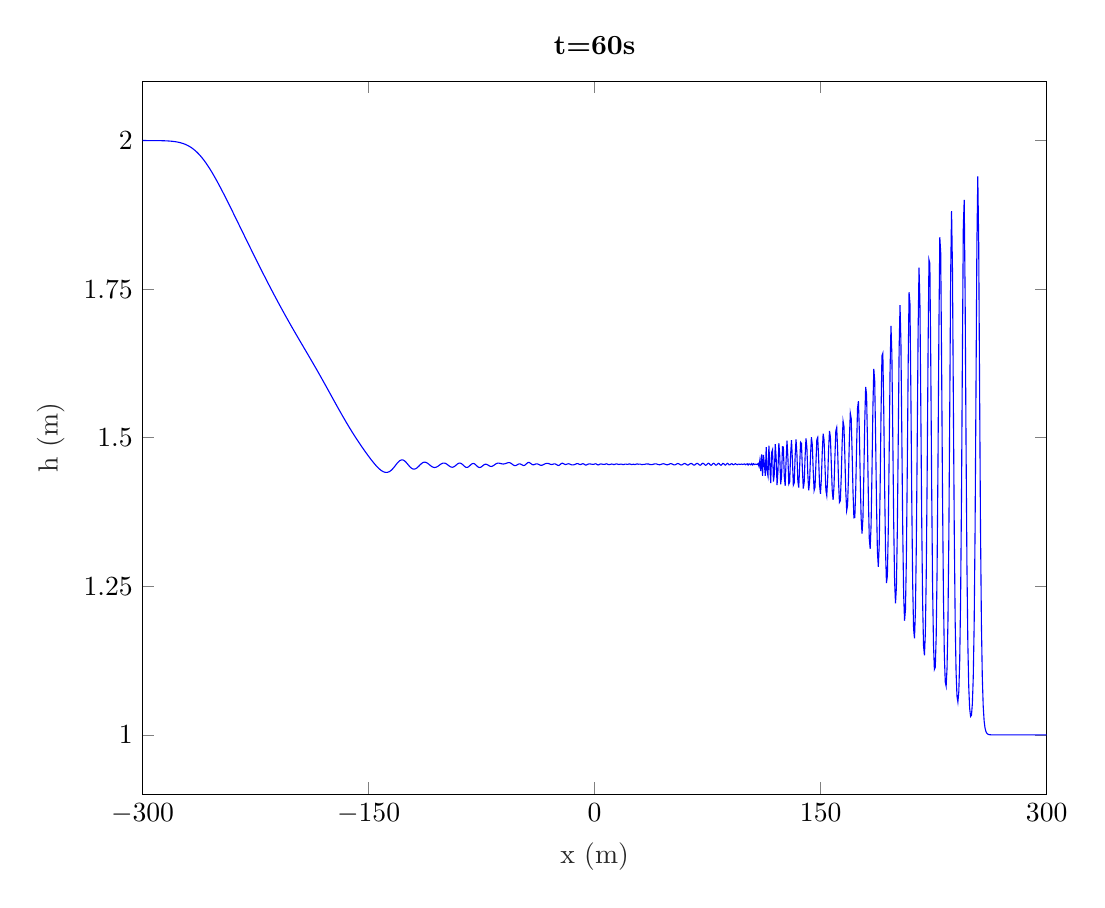
\begin{tikzpicture}

\begin{axis}[%
width=4.521in,
height=3.566in,
at={(0.758in,0.481in)},
scale only axis,
xmin=-300,
xmax=300,
xtick={-300, -150,    0,  150,  300},
xlabel style={font=\color{white!15!black}},
xlabel={x (m)},
ymin=0.9,
ymax=2.1,
ytick={   1, 1.25,  1.5, 1.75,    2},
ylabel style={font=\color{white!15!black}},
ylabel={h (m)},
axis background/.style={fill=white},
title style={font=\bfseries},
title={t=60s}
]
\addplot [color=blue, forget plot]
  table[row sep=crcr]{%
-300.18000900045	2\\
-299.57997899895	1.99998096511179\\
-298.97994899745	1.99998012452313\\
-298.37991899595	1.99997876891258\\
-297.77988899445	1.99997684359111\\
-297.17985899295	1.99997430513158\\
-296.57982899145	1.99997109691597\\
-295.979798989949	1.99996714820747\\
-295.379768988449	1.9999623730339\\
-294.779738986949	1.99995666885899\\
-294.179708985449	1.99994991503437\\
-293.579678983949	1.99994197102433\\
-292.979648982449	1.99993267439581\\
-292.379618980949	1.99992183856605\\
-291.779588979449	1.9999092503009\\
-291.179558977949	1.9998946669584\\
-290.579528976449	1.99987781347329\\
-289.979498974949	1.99985837908067\\
-289.379468973449	1.99983601377999\\
-288.779438971949	1.99981032454363\\
-288.179408970449	1.99978087127936\\
-287.579378968948	1.99974716256043\\
-286.979348967448	1.99970865114346\\
-286.379318965948	1.99966472930092\\
-285.779288964448	1.99961472400276\\
-285.179258962948	1.99955789199029\\
-284.579228961448	1.9994934147945\\
-283.979198959948	1.99942039376137\\
-283.379168958448	1.99933784515675\\
-282.779138956948	1.9992446954346\\
-282.179108955448	1.99913977676314\\
-281.579078953948	1.99902182291435\\
-280.979048952448	1.9988894656324\\
-280.379018950948	1.99874123160609\\
-279.778988949447	1.99857554017794\\
-279.178958947947	1.99839070192918\\
-278.578928946447	1.99818491828293\\
-277.978898944947	1.9979562822689\\
-277.378868943447	1.99770278058996\\
-276.778838941947	1.99742229712415\\
-276.178808940447	1.9971126179842\\
-275.578778938947	1.99677143824057\\
-274.978748937447	1.99639637039273\\
-274.378718935947	1.99598495464674\\
-273.778688934447	1.99553467102583\\
-273.178658932947	1.99504295330396\\
-272.578628931447	1.99450720471213\\
-271.978598929946	1.99392481532256\\
-271.378568928446	1.99329318097008\\
-270.778538926946	1.99260972352182\\
-270.178508925446	1.9918719122597\\
-269.578478923946	1.99107728609489\\
-268.978448922446	1.99022347629251\\
-268.378418920946	1.98930822934905\\
-267.778388919446	1.98832942963749\\
-267.178358917946	1.9872851214158\\
-266.578328916446	1.98617352978626\\
-265.978298914946	1.984993080196\\
-265.378268913446	1.98374241608416\\
-264.778238911946	1.98242041430847\\
-264.178208910446	1.98102619802301\\
-263.578178908945	1.97955914672893\\
-262.978148907445	1.97801890327941\\
-262.378118905945	1.97640537768714\\
-261.778088904445	1.97471874765502\\
-261.178058902945	1.97295945582591\\
-260.578028901445	1.97112820382277\\
-259.977998899945	1.96922594322316\\
-259.377968898445	1.96725386368014\\
-258.777938896945	1.96521337846134\\
-258.177908895445	1.96310610772982\\
-257.577878893945	1.96093385992955\\
-256.977848892445	1.9586986116674\\
-256.377818890945	1.95640248649895\\
-255.777788889444	1.95404773302959\\
-255.177758887944	1.95163670273403\\
-254.577728886444	1.94917182787929\\
-253.977698884944	1.94665559990768\\
-253.377668883444	1.94409054860142\\
-252.777638881944	1.94147922230859\\
-252.177608880444	1.938824169465\\
-251.577578878944	1.93612792159886\\
-250.977548877444	1.93339297795734\\
-250.377518875944	1.93062179184696\\
-249.777488874444	1.92781675873586\\
-249.177458872944	1.92498020612509\\
-248.577428871444	1.92211438515975\\
-247.977398869943	1.91922146391981\\
-247.377368868443	1.91630352230417\\
-246.777338866943	1.91336254840129\\
-246.177308865443	1.91040043622417\\
-245.577278863943	1.90741898467715\\
-244.977248862443	1.90441989761635\\
-244.377218860943	1.90140478486372\\
-243.777188859443	1.89837516403642\\
-243.177158857943	1.89533246305783\\
-242.577128856443	1.89227802322371\\
-241.977098854943	1.88921310270539\\
-241.377068853443	1.88613888038196\\
-240.777038851943	1.88305645990437\\
-240.177008850443	1.8799668739049\\
-239.576978848942	1.87687108827703\\
-238.976948847442	1.87377000646125\\
-238.376918845942	1.87066447368268\\
-237.776888844442	1.86755528109605\\
-237.176858842942	1.86444316980237\\
-236.576828841442	1.8613288347096\\
-235.976798839942	1.8582129282168\\
-235.376768838442	1.85509606370714\\
-234.776738836942	1.851978818841\\
-234.176708835442	1.84886173864434\\
-233.576678833942	1.84574533839146\\
-232.976648832442	1.84263010628447\\
-232.376618830942	1.83951650593383\\
-231.776588829441	1.83640497864621\\
-231.176558827941	1.83329594552755\\
-230.576528826441	1.83018980940958\\
-229.976498824941	1.82708695660894\\
-229.376468823441	1.82398775852813\\
-228.776438821941	1.82089257310758\\
-228.176408820441	1.81780174613776\\
-227.576378818941	1.81471561244005\\
-226.976348817441	1.81163449692439\\
-226.376318815941	1.80855871553142\\
-225.776288814441	1.80548857606587\\
-225.176258812941	1.80242437892757\\
-224.576228811441	1.79936641774543\\
-223.976198809941	1.79631497991942\\
-223.37616880844	1.79327034707454\\
-222.77613880694	1.79023279543023\\
-222.17610880544	1.7872025960881\\
-221.57607880394	1.78418001523999\\
-220.97604880244	1.78116531429811\\
-220.37601880094	1.77815874994806\\
-219.77598879944	1.77516057412542\\
-219.17595879794	1.77217103391578\\
-218.57592879644	1.76919037137792\\
-217.97589879494	1.7662188232893\\
-217.37586879344	1.76325662081288\\
-216.77583879194	1.76030398908378\\
-216.17580879044	1.75736114671448\\
-215.575778788939	1.75442830521668\\
-214.975748787439	1.75150566833844\\
-214.375718785939	1.74859343131465\\
-213.775688784439	1.74569178002965\\
-213.175658782939	1.74280089009062\\
-212.575628781439	1.73992092581088\\
-211.975598779939	1.73705203910278\\
-211.375568778439	1.73419436828048\\
-210.775538776939	1.73134803677344\\
-210.175508775439	1.7285131517529\\
-209.575478773939	1.72568980267416\\
-208.975448772439	1.72287805973917\\
-208.375418770939	1.72007797228525\\
-207.775388769438	1.71728956710736\\
-207.175358767938	1.71451284672351\\
-206.575328766438	1.7117477875945\\
-205.975298764938	1.70899433831192\\
-205.375268763438	1.70625241777044\\
-204.775238761938	1.70352191334316\\
-204.175208760438	1.70080267908147\\
-203.575178758938	1.69809453396377\\
-202.975148757438	1.69539726022014\\
-202.375118755938	1.69271060176309\\
-201.775088754438	1.6900342627571\\
-201.175058752938	1.68736790636263\\
-200.575028751438	1.68471115369232\\
-199.974998749937	1.68206358301931\\
-199.374968748437	1.67942472927937\\
-198.774938746937	1.6767940839092\\
-198.174908745437	1.6741710950639\\
-197.574878743937	1.67155516825582\\
-196.974848742437	1.6689456674558\\
-196.374818740937	1.66634191669501\\
-195.774788739437	1.66374320220212\\
-195.174758737937	1.66114877510541\\
-194.574728736437	1.65855785472318\\
-193.974698734937	1.65596963245848\\
-193.374668733437	1.65338327630482\\
-192.774638731937	1.65079793595979\\
-192.174608730437	1.64821274853228\\
-191.574578728936	1.6456268448163\\
-190.974548727436	1.64303935609229\\
-190.374518725936	1.64044942140276\\
-189.774488724436	1.63785619523616\\
-189.174458722936	1.63525885553961\\
-188.574428721436	1.63265661196869\\
-187.974398719936	1.63004871427144\\
-187.374368718436	1.62743446069366\\
-186.774338716936	1.62481320628549\\
-186.174308715436	1.62218437098342\\
-185.574278713936	1.6195474473397\\
-184.974248712436	1.61690200777127\\
-184.374218710936	1.61424771120392\\
-183.774188709435	1.61158430899405\\
-183.174158707935	1.60891165002005\\
-182.574128706435	1.60622968484827\\
-181.974098704935	1.60353846889324\\
-181.374068703435	1.60083816450977\\
-180.774038701935	1.59812904197352\\
-180.174008700435	1.59541147932632\\
-179.573978698935	1.59268596108386\\
-178.973948697435	1.58995307582313\\
-178.373918695935	1.5872135126867\\
-177.773888694435	1.58446805685897\\
-177.173858692935	1.58171758408541\\
-176.573828691435	1.57896305431925\\
-175.973798689934	1.57620550459085\\
-175.373768688434	1.57344604120242\\
-174.773738686934	1.57068583135547\\
-174.173708685434	1.5679260943195\\
-173.573678683934	1.56516809224911\\
-172.973648682434	1.5624131207527\\
-172.373618680934	1.55966249930946\\
-171.773588679434	1.55691756162356\\
-171.173558677934	1.55417964599532\\
-170.573528676434	1.55145008577932\\
-169.973498674934	1.5487301999901\\
-169.373468673434	1.5460212841069\\
-168.773438671934	1.54332460112149\\
-168.173408670434	1.54064137286708\\
-167.573378668933	1.53797277166301\\
-166.973348667433	1.53531991230901\\
-166.373318665933	1.5326838444652\\
-165.773288664433	1.53006554545996\\
-165.173258662933	1.52746591357657\\
-164.573228661433	1.52488576188293\\
-163.973198659933	1.52232581268464\\
-163.373168658433	1.51978669270159\\
-162.773138656933	1.51726892909084\\
-162.173108655433	1.51477294646357\\
-161.573078653933	1.512299065071\\
-160.973048652433	1.50984750036181\\
-160.373018650933	1.50741836414158\\
-159.772988649432	1.5050116675911\\
-159.172958647932	1.50262732642464\\
-158.572928646432	1.50026516848897\\
-157.972898644932	1.4979249441186\\
-157.372868643432	1.49560633956992\\
-156.772838641932	1.49330899385589\\
-156.172808640432	1.49103251929226\\
-155.572778638932	1.48877652604438\\
-154.972748637432	1.48654065093099\\
-154.372718635932	1.48432459069661\\
-153.772688634432	1.48212813990839\\
-153.172658632932	1.47995123356726\\
-152.572628631432	1.47779399444791\\
-151.972598629931	1.47565678510015\\
-151.372568628431	1.47354026435634\\
-150.772538626931	1.47144544809827\\
-150.172508625431	1.46937377394252\\
-149.572478623931	1.46732716940582\\
-148.972448622431	1.4653081230075\\
-148.372418620931	1.46331975764993\\
-147.772388619431	1.46136590547925\\
-147.172358617931	1.45945118325151\\
-146.572328616431	1.45758106699338\\
-145.972298614931	1.45576196442102\\
-145.372268613431	1.45400128312932\\
-144.772238611931	1.45230749194142\\
-144.172208610431	1.45069017196153\\
-143.57217860893	1.44916005274724\\
-142.97214860743	1.44772902754991\\
-142.37211860593	1.44641013971679\\
-141.77208860443	1.44521753007387\\
-141.17205860293	1.44416633242962\\
-140.57202860143	1.44327250133677\\
-139.97199859993	1.44255255311757\\
-139.37196859843	1.4420231982529\\
-138.77193859693	1.44170084113554\\
-138.17190859543	1.4416009888028\\
-137.57187859393	1.44173708728643\\
-136.97184859243	1.4421201413203\\
-136.37181859093	1.4427568402948\\
-135.771788589429	1.44364847721122\\
-135.171758587929	1.44478935275823\\
-134.571728586429	1.44616520646449\\
-133.971698584929	1.44775174816464\\
-133.371668583429	1.44951347985233\\
-132.771638581929	1.45140304256184\\
-132.171608580429	1.45336134951277\\
-131.571578578929	1.45531875865001\\
-130.971548577429	1.45719747808758\\
-130.371518575929	1.45891527975958\\
-129.771488574429	1.46039041927222\\
-129.171458572929	1.46154744560949\\
-128.571428571429	1.46232337093488\\
-127.971398569929	1.46267350919456\\
-127.371368568428	1.46257622274637\\
-126.771338566928	1.46203595243727\\
-126.171308565428	1.46108396741261\\
-125.571278563928	1.45977680029398\\
-124.971248562428	1.4581924851675\\
-124.371218560928	1.45642509744959\\
-123.771188559428	1.45457825545497\\
-123.171158557928	1.45275828739354\\
-122.571128556428	1.45106768000434\\
-121.971098554928	1.44959925375373\\
-121.371068553428	1.44843131425289\\
-120.771038551928	1.44762385255708\\
-120.171008550428	1.44721574954958\\
-119.570978548927	1.44722291032005\\
-118.970948547427	1.44763725761509\\
-118.370918545927	1.44842667798786\\
-117.770888544427	1.44953599076606\\
-117.170858542927	1.45088919540517\\
-116.570828541427	1.4523931986239\\
-115.970798539927	1.45394315886765\\
-115.370768538427	1.45542939411738\\
-114.770738536927	1.45674550422445\\
-114.170708535427	1.45779705939227\\
-113.570678533927	1.45850991934109\\
-112.970648532427	1.45883712941189\\
-112.370618530927	1.45876339841903\\
-111.770588529426	1.45830649446754\\
-111.170558527926	1.45751526006535\\
-110.570528526426	1.45646459656362\\
-109.970498524926	1.45524810983125\\
-109.370468523426	1.4539694257655\\
-108.770438521926	1.45273323597537\\
-108.170408520426	1.45163697511775\\
-107.570378518926	1.45076377525684\\
-106.970348517426	1.45017702608032\\
-106.370318515926	1.44991662377287\\
-105.770288514426	1.44999682753707\\
-105.170258512926	1.45040557087612\\
-104.570228511426	1.45110520213359\\
-103.970198509925	1.45203459553562\\
-103.370168508425	1.45311276440055\\
-102.770138506925	1.45424409465052\\
-102.170108505425	1.45532524108899\\
-101.570078503925	1.45625354099299\\
-100.970048502425	1.45693649232101\\
-100.370018500925	1.45730149104771\\
-99.769988499425	1.45730471010118\\
-99.1699584979249	1.45693788974711\\
-98.5699284964248	1.45623177708672\\
-97.9698984949247	1.45525543280287\\
-97.3698684934247	1.45411101722284\\
-96.7698384919246	1.45292433249563\\
-96.1698084904245	1.451831944864\\
-95.5697784889244	1.45096611207901\\
-94.9697484874244	1.45043896760859\\
-94.3697184859243	1.45032756948701\\
-93.7696884844242	1.45066141781107\\
-93.1696584829241	1.45141427297774\\
-92.5696284814241	1.45250195181763\\
-91.969598479924	1.45378776875001\\
-91.3695684784239	1.45509657327919\\
-90.7695384769239	1.45623709615062\\
-90.1695084754238	1.45703045591452\\
-89.5694784739237	1.45734089936294\\
-88.9694484724236	1.45710085962716\\
-88.3694184709235	1.45633069383836\\
-87.7693884694235	1.45513778921538\\
-87.1693584679234	1.45370415118448\\
-86.5693284664233	1.45225793390806\\
-85.9692984649232	1.45103594389116\\
-85.3692684634232	1.45024334912512\\
-84.7692384619231	1.45001741403257\\
-84.169208460423	1.45040056043625\\
-83.5691784589229	1.45132923746135\\
-82.9691484574229	1.45263878328517\\
-82.3691184559228	1.45408831477432\\
-81.7690884544227	1.45540198491634\\
-81.1690584529227	1.45632127126939\\
-80.5690284514226	1.45665837746067\\
-79.9689984499225	1.45633741240319\\
-79.3689684484224	1.45541529003957\\
-78.7689384469223	1.45407091401818\\
-78.1689084454223	1.45256930797199\\
-77.5688784439222	1.45120597496835\\
-76.9688484424221	1.45024534707352\\
-76.368818440922	1.44986618527193\\
-75.768788439422	1.45012689769441\\
-75.1687584379219	1.45095132503324\\
-74.5687284364218	1.45214809327125\\
-73.9686984349217	1.45345056238813\\
-73.3686684334217	1.45457622941266\\
-72.7686384319216	1.45529097155201\\
-72.1686084304215	1.45546295881249\\
-71.5685784289215	1.45509201586007\\
-70.9685484274214	1.45430610065019\\
-70.3685184259213	1.45332628666719\\
-69.7684884244212	1.4524103770867\\
-69.1684584229211	1.4517908896406\\
-68.5684284214211	1.45162321679908\\
-67.968398419921	1.45195523300638\\
-67.3683684184209	1.45272450573688\\
-66.7683384169208	1.45378014661706\\
-66.1683084154208	1.45492371106598\\
-65.5682784139207	1.45595731993374\\
-64.9682484124206	1.45672708138562\\
-64.3682184109205	1.45715149102592\\
-63.7681884094205	1.45722945951766\\
-63.1681584079204	1.45702898447372\\
-62.5681284064203	1.45666279870874\\
-61.9680984049203	1.45625972756382\\
-61.3680684034202	1.45593916617868\\
-60.7680384019201	1.45579245343547\\
-60.16800840042	1.45587104031505\\
-59.5679783989199	1.4561794138906\\
-58.9679483974199	1.45667122022384\\
-58.3679183959198	1.45724989662608\\
-57.7678883944197	1.45777771573552\\
-57.1678583929196	1.45809770367111\\
-56.5678283914196	1.45806947961875\\
-55.9677983899195	1.4576132630667\\
-55.3677683884194	1.45674873808965\\
-54.7677383869193	1.45561187124738\\
-54.1677083854193	1.45443626199292\\
-53.5676783839192	1.45349672223065\\
-52.9676483824191	1.45302750205111\\
-52.3676183809191	1.45314010060454\\
-51.767588379419	1.45377071553341\\
-51.1675583779189	1.45468277022139\\
-50.5675283764188	1.45553402524106\\
-49.9674983749187	1.45599416728796\\
-49.3674683734187	1.45587370127449\\
-48.7674383719186	1.45521171604135\\
-48.1674083704185	1.45427891699449\\
-47.5673783689184	1.45348543101486\\
-46.9673483674184	1.45322374735478\\
-46.3673183659183	1.45370620705115\\
-45.7672883644182	1.45486546764537\\
-45.1672583629181	1.45635953374566\\
-44.5672283614181	1.457692759299\\
-43.967198359918	1.45840981882047\\
-43.3671683584179	1.45828416842106\\
-42.7671383569178	1.45741445350437\\
-42.1671083554178	1.45617944914789\\
-41.5670783539177	1.45507019826793\\
-40.9670483524176	1.45447733739874\\
-40.3670183509175	1.45453105370705\\
-39.7669883494175	1.45506341192411\\
-39.1669583479174	1.45570587677011\\
-38.5669283464173	1.45607291562734\\
-37.9668983449172	1.4559427866342\\
-37.3668683434172	1.45534865265679\\
-36.7668383419171	1.4545411306749\\
-36.166808340417	1.45385287186348\\
-35.5667783389169	1.45354356976289\\
-34.9667483374168	1.45370383395471\\
-34.3667183359168	1.45425265299111\\
-33.7666883344167	1.45500820094367\\
-33.1666583329167	1.45577576821778\\
-32.5666283314166	1.45640242868434\\
-31.9665983299165	1.45678506715502\\
-31.3665683284164	1.45685921764564\\
-30.7665383269164	1.45660695285413\\
-30.1665083254163	1.45609258248931\\
-29.5664783239162	1.45549006923881\\
-28.9664483224161	1.45504832363298\\
-28.3664183209161	1.45497607547894\\
-27.766388319416	1.45529807877079\\
-27.1663583179159	1.45578575834236\\
-26.5663283164158	1.45604675799757\\
-25.9662983149157	1.45575814437738\\
-25.3662683134157	1.45491585065733\\
-24.7662383119156	1.45390703389737\\
-24.1662083104155	1.45332245991889\\
-23.5661783089154	1.45359099682734\\
-22.9661483074154	1.45467179752124\\
-22.3661183059153	1.45602881229286\\
-21.7660883044152	1.45694225630792\\
-21.1660583029151	1.45697119213356\\
-20.5660283014151	1.45624299474175\\
-19.965998299915	1.45534582173308\\
-19.3659682984149	1.45489724248195\\
-18.7659382969148	1.45511420494923\\
-18.1659082954148	1.45570182867187\\
-17.5658782939147	1.45612666550535\\
-16.9658482924146	1.45603513444178\\
-16.3658182909145	1.45547991658646\\
-15.7657882894144	1.45480270955008\\
-15.1657582879144	1.45433373697381\\
-14.5657282864143	1.45420054613748\\
-13.9656982849143	1.45437312916483\\
-13.3656682834142	1.45480448692711\\
-12.7656382819141	1.45544337951855\\
-12.165608280414	1.45610844945466\\
-11.565578278914	1.45645195777874\\
-10.9655482774139	1.45619560367997\\
-10.3655182759138	1.45547903074855\\
-9.76548827441371	1.4548842537326\\
-9.16545827291367	1.45496512014923\\
-8.56542827141357	1.45566305905457\\
-7.96539826991352	1.45625915850587\\
-7.36536826841342	1.45604074306228\\
-6.76533826691332	1.45505869541237\\
-6.16530826541327	1.45413127018175\\
-5.56527826391317	1.45403130977902\\
-4.96524826241313	1.45473594076468\\
-4.36521826091303	1.45555761842695\\
-3.76518825941298	1.45593090923023\\
-3.16515825791288	1.4558755783297\\
-2.56512825641283	1.45568015124751\\
-1.96509825491273	1.45544573719641\\
-1.36506825341269	1.4551947546117\\
-0.765038251912586	1.45518267928121\\
-0.165008250412541	1.45561783785862\\
0.435021751087561	1.45608476983133\\
1.03505175258761	1.45582530740882\\
1.63508175408771	1.45484810530199\\
2.23511175558775	1.45418443739162\\
2.83514175708785	1.4545774710407\\
3.43517175858796	1.45545350733395\\
4.035201760088	1.45583192003157\\
4.6352317615881	1.45565788891348\\
5.23526176308815	1.45542394087985\\
5.83529176458825	1.45519281250922\\
6.43532176608829	1.45503855176335\\
7.03535176758839	1.45544081563891\\
7.63538176908844	1.45610876771084\\
8.23541177058854	1.45592037425446\\
8.83544177208859	1.45501695858739\\
9.43547177358869	1.45467407545499\\
10.0355017750887	1.45494425579779\\
10.6355317765888	1.45527296018484\\
11.2355617780889	1.45571213926819\\
11.835591779589	1.45558800051065\\
12.435621781089	1.45487919613491\\
13.0356517825891	1.4549259876162\\
13.6356817840892	1.45537811844331\\
14.2357117855893	1.45586898831805\\
14.8357417870894	1.45589040263603\\
15.4357717885894	1.45526808530278\\
16.0358017900895	1.45495274525947\\
16.6358317915896	1.45519947174205\\
17.2358617930897	1.45565338582587\\
17.8358917945897	1.45558343886957\\
18.4359217960898	1.45500936331882\\
19.0359517975899	1.45471521518322\\
19.63598179909	1.45510464708242\\
20.23601180059	1.45566378236246\\
20.8360418020901	1.45563196525253\\
21.4360718035902	1.45519677066382\\
22.0361018050903	1.45522611596982\\
22.6361318065904	1.45571252032042\\
23.2361618080904	1.45587979186133\\
23.8361918095905	1.45534462244898\\
24.4362218110905	1.45482899701399\\
25.0362518125906	1.45504676740452\\
25.6362818140907	1.45538985759974\\
26.2363118155908	1.4550991098705\\
26.8363418170908	1.45483597240713\\
27.4363718185909	1.45537498917005\\
28.036401820091	1.45594552931126\\
28.6364318215911	1.45568648122169\\
29.2364618230911	1.45537181547819\\
29.8364918245912	1.4556448487039\\
30.4365218260913	1.45553735592576\\
31.0365518275914	1.45480036076751\\
31.6365818290914	1.45472347318099\\
32.2366118305915	1.45516853649119\\
32.8366418320916	1.45505015173557\\
33.4366718335917	1.45521559189978\\
34.0367018350918	1.45591586595909\\
34.6367318365918	1.45582407304328\\
35.2367618380919	1.45571448410105\\
35.836791839592	1.45571187740332\\
36.4368218410921	1.45496666045349\\
37.0368518425921	1.45488908295192\\
37.6368818440922	1.45468078082608\\
38.2369118455923	1.45488610846305\\
38.8369418470924	1.45523342071408\\
39.4369718485924	1.45568152578715\\
40.0370018500925	1.4559831526178\\
40.6370318515926	1.4560230037951\\
41.2370618530927	1.45568624611515\\
41.8370918545928	1.45514367405893\\
42.4371218560928	1.45467503254922\\
43.0371518575929	1.45451377793692\\
43.6371818590929	1.45479061675747\\
44.237211860593	1.45531620263869\\
44.8372418620931	1.45587010063155\\
45.4372718635932	1.45616703347042\\
46.0373018650932	1.45601975346843\\
46.6373318665933	1.45555030921918\\
47.2373618680934	1.45489925561427\\
47.8373918695935	1.45444106846605\\
48.4374218710935	1.45446551477461\\
49.0374518725936	1.45495039948056\\
49.6374818740937	1.45569592220036\\
50.2375118755938	1.45629434875748\\
50.8375418770938	1.45632122781245\\
51.4375718785939	1.45573573266219\\
52.037601880094	1.45489806284658\\
52.6376318815941	1.45428360979604\\
53.2376618830942	1.45427007845097\\
53.8376918845942	1.45493377048787\\
54.4377218860943	1.45589312337252\\
55.0377518875944	1.45650268240329\\
55.6377818890945	1.45634180932577\\
56.2378118905945	1.45552315085726\\
56.8378418920946	1.45457361108468\\
57.4378718935947	1.45408893465387\\
58.0379018950948	1.45440293799731\\
58.6379318965948	1.45536352703323\\
59.2379618980949	1.45635140094822\\
59.837991899595	1.45664895492417\\
60.4380219010951	1.45598597662695\\
61.0380519025952	1.45481126388389\\
61.6380819040952	1.45399271755739\\
62.2381119055953	1.45415646002344\\
62.8381419070953	1.45519993210808\\
63.4381719085955	1.45635277974548\\
64.0382019100955	1.45673902857211\\
64.6382319115956	1.45603980272779\\
65.2382619130956	1.45476104335966\\
65.8382919145957	1.45389008444227\\
66.4383219160958	1.454148565374\\
67.0383519175959	1.45538626460836\\
67.6383819190959	1.45662431049045\\
68.238411920596	1.45680541652969\\
68.8384419220961	1.45570962811415\\
69.4384719235962	1.4542304838874\\
70.0385019250962	1.45366831072715\\
70.6385319265963	1.4545780793309\\
71.2385619280964	1.45620149384761\\
71.8385919295965	1.45706215263992\\
72.4386219310966	1.45631216136187\\
73.0386519325966	1.4546101669108\\
73.6386819340967	1.45356848552347\\
74.2387119355968	1.45422595007742\\
74.8387419370969	1.45597146082456\\
75.4387719385969	1.45706555014236\\
76.038801940097	1.45636916219928\\
76.6388319415971	1.45458921091063\\
77.2388619430972	1.45361065458479\\
77.8388919445972	1.45450901569171\\
78.4389219460973	1.45630825594743\\
79.0389519475974	1.45698218172373\\
79.6389819490975	1.45572308266207\\
80.2390119505975	1.45397395342801\\
80.8390419520976	1.45382179261461\\
81.4390719535977	1.45549865153673\\
82.0391019550977	1.45698725877607\\
82.6391319565979	1.45641763274447\\
83.2391619580979	1.45448323090575\\
83.839191959598	1.45366060325461\\
84.439221961098	1.45501652192196\\
85.0392519625981	1.456713456\\
85.6392819640982	1.45641960948473\\
86.2393119655983	1.45457779958429\\
86.8393419670983	1.45387326380761\\
87.4393719685984	1.45535260592234\\
88.0394019700985	1.45680158711249\\
88.6394319715986	1.45600708957325\\
89.2394619730986	1.45422383521335\\
89.8394919745987	1.45423685370401\\
90.4395219760988	1.4558817278652\\
91.0395519775989	1.45635069432337\\
91.639581979099	1.45500034490015\\
92.239611980599	1.45441184217063\\
92.8396419820991	1.45561956207755\\
93.4396719835992	1.4562414420927\\
94.0397019850993	1.455153914699\\
94.6397319865993	1.45461564343193\\
95.2397619880994	1.45548353509639\\
95.8397919895995	1.455628853521\\
96.4398219910996	1.45494687252322\\
97.0398519925996	1.45531460217652\\
97.6398819940997	1.45566706166712\\
98.2399119955998	1.45501532076596\\
98.8399419970999	1.45545333320943\\
99.4399719985999	1.45585908678891\\
100.0400020001	1.45459022643562\\
100.6400320016	1.45541157518207\\
101.2400620031	1.45612710986567\\
101.8400920046	1.45403321126555\\
102.4401220061	1.45605206376998\\
103.0401520076	1.45546481959085\\
103.6401820091	1.45440514768698\\
104.240212010601	1.45654151626207\\
104.840242012101	1.45425816694102\\
105.440272013601	1.45615523014446\\
106.040302015101	1.4549143640413\\
106.640332016601	1.45557086676829\\
107.240362018101	1.45530332493646\\
107.840392019601	1.45495142223821\\
108.440422021101	1.45659947219329\\
109.040452022601	1.45184425749707\\
109.640482024101	1.46221131790412\\
110.240512025601	1.44371892809531\\
110.840542027101	1.47193008147499\\
111.440572028601	1.43592905859334\\
112.040602030102	1.47120294245516\\
112.640632031602	1.45427769810935\\
113.240662033102	1.43602867067227\\
113.840692034602	1.48414706257872\\
114.440722036102	1.44335192481957\\
115.040752037602	1.43523706979857\\
115.640782039102	1.48656465436251\\
116.240812040602	1.45299571556236\\
116.840842042102	1.42378882084692\\
117.440872043602	1.47504163451985\\
118.040902045102	1.47955863489755\\
118.640932046602	1.42622732390513\\
119.240962048102	1.43897624279664\\
119.840992049603	1.48929494947843\\
120.441022051103	1.46690309735418\\
121.041052052603	1.42035213515009\\
121.641082054103	1.44403306213667\\
122.241112055603	1.49099650561388\\
122.841142057103	1.46944583881679\\
123.441172058603	1.4217140984305\\
124.041202060103	1.43448596957396\\
124.641232061603	1.48475740490117\\
125.241262063103	1.48439718663761\\
125.841292064603	1.43487439736736\\
126.441322066103	1.4192230665944\\
127.041352067603	1.46124042081616\\
127.641382069103	1.49494754864487\\
128.241412070604	1.46707483834196\\
128.841442072104	1.42198450682126\\
129.441472073604	1.42557239106395\\
130.041502075104	1.47210530699934\\
130.641532076604	1.4957262756786\\
131.241562078104	1.46251977434977\\
131.841592079604	1.42021280062323\\
132.441622081104	1.4240762279493\\
133.041652082604	1.46868541638844\\
133.641682084104	1.49700792542939\\
134.241712085604	1.47207062938353\\
134.841742087104	1.4268211770734\\
135.441772088604	1.41600167782593\\
136.041802090105	1.45135152821209\\
136.641832091605	1.49245914804709\\
137.241862093105	1.490481568136\\
137.841892094605	1.44823309243899\\
138.441922096105	1.41440593859889\\
139.041952097605	1.42432356935621\\
139.641982099105	1.46765066729996\\
140.242012100605	1.49897951355077\\
140.842042102105	1.48396391968634\\
141.442072103605	1.43946847174855\\
142.042102105105	1.41132224458989\\
142.642132106605	1.42574990438427\\
143.242162108105	1.46945493289034\\
143.842192109605	1.50072655489529\\
144.442222111106	1.48799863744156\\
145.042252112606	1.44433489536074\\
145.642282114106	1.41114718888986\\
146.242312115606	1.41680474307868\\
146.842342117106	1.4566227413264\\
147.442372118606	1.49677866292063\\
148.042402120106	1.50055017141631\\
148.642432121606	1.46439404227624\\
149.242462123106	1.4209515596838\\
149.842492124606	1.40555946559536\\
150.442522126106	1.42983496081171\\
151.042552127606	1.47584228794082\\
151.642582129106	1.50689403918628\\
152.242612130607	1.49611925864461\\
152.842642132107	1.452683494135\\
153.442672133607	1.41163353167136\\
154.042702135107	1.40255641489717\\
154.642732136607	1.43169593857314\\
155.242762138107	1.4797974635387\\
155.842792139607	1.51155366871591\\
156.442822141107	1.50128867797014\\
157.042852142607	1.45690237864309\\
157.642882144107	1.41158201961709\\
158.242912145607	1.39540306868147\\
158.842942147107	1.41855388291124\\
159.442972148607	1.467832154773\\
160.043002150107	1.51140039389809\\
160.643032151608	1.51719900349641\\
161.243062153108	1.48009466589485\\
161.843092154608	1.42664317218699\\
162.443122156108	1.39118162497337\\
163.043152157608	1.39389183573436\\
163.643182159108	1.4342616578452\\
164.243212160608	1.49086506639056\\
164.843242162108	1.52806208339583\\
165.443272163608	1.51880259803891\\
166.043302165108	1.46867729511806\\
166.643332166608	1.41050900099403\\
167.243362168108	1.37747556754542\\
167.843392169608	1.38629969980863\\
168.443422171109	1.43429881267855\\
169.043452172609	1.49866110814868\\
169.643482174109	1.54141217843809\\
170.243512175609	1.53252571368677\\
170.843542177109	1.47667395631372\\
171.443572178609	1.40879511428803\\
172.043602180109	1.36519010256849\\
172.643632181609	1.36566650681963\\
173.243662183109	1.41174848546295\\
173.843692184609	1.48563172501301\\
174.443722186109	1.54932044723374\\
175.043752187609	1.56153349515155\\
175.643782189109	1.5119057078671\\
176.24381219061	1.43151362935218\\
176.84384219211	1.3640924344572\\
177.44387219361	1.33867401671366\\
178.04390219511	1.36536355992193\\
178.64393219661	1.4375892598659\\
179.24396219811	1.52727131236323\\
179.84399219961	1.58561984438449\\
180.44402220111	1.57240902552822\\
181.04405220261	1.49442168500915\\
181.64408220411	1.3984821654535\\
182.24411220561	1.33015702487504\\
182.84414220711	1.31313182955903\\
183.44417220861	1.3536065275218\\
184.04420221011	1.4431314003737\\
184.644232211611	1.54962212508049\\
185.244262213111	1.61585525114627\\
185.844292214611	1.59567187879225\\
186.444322216111	1.500834270281\\
187.044352217611	1.38810510067562\\
187.644382219111	1.30770761108656\\
188.244412220611	1.28292100148596\\
188.844442222111	1.32013855722793\\
189.444472223611	1.4147562806328\\
190.044502225111	1.54061836249153\\
190.644532226611	1.63791736573652\\
191.244562228111	1.64210522710069\\
191.844592229611	1.54785402480133\\
192.444622231112	1.41528981874701\\
193.044652232612	1.30769445091497\\
193.644682234112	1.25556747475511\\
194.244712235612	1.26709681858166\\
194.844742237112	1.3432100491703\\
195.444772238612	1.47340852517269\\
196.044802240112	1.61456580874639\\
196.644832241612	1.68800891133194\\
197.244862243112	1.6398958006951\\
197.844892244612	1.50316908269412\\
198.444922246112	1.35800149094703\\
199.044952247612	1.25847038691727\\
199.644982249112	1.22124723842626\\
200.245012250613	1.24868994619814\\
200.845042252113	1.34206678522723\\
201.445072253613	1.49139663386938\\
202.045102255113	1.64824173474349\\
202.645132256613	1.72314354278974\\
203.245162258113	1.66004599353088\\
203.845192259613	1.5037083270794\\
204.445222261113	1.34460048255555\\
205.045252262613	1.23665555004186\\
205.645282264113	1.19208648963634\\
206.245312265613	1.21024188039926\\
206.845342267113	1.29359511917519\\
207.445372268613	1.44131893052085\\
208.045402270114	1.62081000899419\\
208.645432271614	1.74486657763689\\
209.245462273114	1.72548646253416\\
209.845492274614	1.57617089947911\\
210.445522276114	1.39406621869125\\
211.045552277614	1.25437651022763\\
211.645582279114	1.17820712993786\\
212.245612280614	1.1624903765694\\
212.845642282114	1.20590347778808\\
213.445672283614	1.31452730059629\\
214.045702285114	1.48692949265293\\
214.645732286614	1.67861122739543\\
215.245762288114	1.78611831619234\\
215.845792289614	1.72877630143801\\
216.445822291115	1.54986069112453\\
217.045852292615	1.35922305511905\\
217.645882294115	1.22261480279717\\
218.245912295615	1.15020509434048\\
218.845942297115	1.13374284656624\\
219.445972298615	1.17044658237417\\
220.046002300115	1.26818185759332\\
220.646032301615	1.4344460281281\\
221.246062303115	1.64305074688502\\
221.846092304615	1.79955131392349\\
222.446122306115	1.79322976068854\\
223.046152307615	1.62826857216363\\
223.646182309115	1.41788144199631\\
224.246212310616	1.25213658979748\\
224.846242312116	1.15290953587868\\
225.446272313616	1.11012710839835\\
226.046302315116	1.11386793141892\\
226.646332316616	1.16571796329421\\
227.246362318116	1.27826590253549\\
227.846392319616	1.4610667337189\\
228.446422321116	1.68291745268565\\
229.046452322616	1.83736119446983\\
229.646482324116	1.81112083993047\\
230.246512325616	1.62478284545225\\
230.846542327116	1.4040233680234\\
231.446572328616	1.23611543281866\\
232.046602330116	1.13606856840141\\
232.646632331617	1.08915904679456\\
233.246662333117	1.08201409540352\\
233.846692334617	1.1125019604151\\
234.446722336117	1.19095894057358\\
235.046752337617	1.33530324290766\\
235.646782339117	1.54916537258948\\
236.246812340617	1.77512869938528\\
236.846842342117	1.88125012435795\\
237.446872343617	1.78339048255909\\
238.046902345117	1.55879748182921\\
238.646932346617	1.34088508791549\\
239.246962348117	1.1906819719181\\
239.846992349617	1.10529020740915\\
240.447022351118	1.06488806453296\\
241.047052352618	1.05524015333686\\
241.647082354118	1.07263267110128\\
242.247112355618	1.12429681861402\\
242.847142357118	1.22789538709311\\
243.447172358618	1.40354953166148\\
244.047202360118	1.64251382397578\\
244.647232361618	1.85614790496465\\
245.247262363118	1.90022705534913\\
245.847292364618	1.73792412038276\\
246.447322366118	1.49229132305342\\
247.047352367618	1.285993373329\\
247.647382369118	1.15386601997065\\
248.247412370619	1.08082753800974\\
248.847442372119	1.04476311319044\\
249.447472373619	1.03093840239236\\
250.047502375119	1.03306423259042\\
250.647532376619	1.05226423045016\\
251.247562378119	1.0974221181772\\
251.847592379619	1.18648057099778\\
252.447622381119	1.34339643520219\\
253.047652382619	1.57603990805515\\
253.647682384119	1.82381261727551\\
254.247712385619	1.93977490903217\\
254.847742387119	1.82992114073987\\
255.447772388619	1.58343863645811\\
256.04780239012	1.34855934417702\\
256.64783239162	1.18865402179978\\
257.24786239312	1.09673303882583\\
257.84789239462	1.04823491024864\\
258.44792239612	1.02371825073109\\
259.04795239762	1.01158292059508\\
259.64798239912	1.00563763357867\\
260.24801240062	1.00273948720696\\
260.84804240212	1.00133015252384\\
261.44807240362	1.00064561178849\\
262.04810240512	1.00031330393793\\
262.64813240662	1.00015202908801\\
263.24816240812	1.00007376908364\\
263.84819240962	1.00003579471291\\
264.448222411121	1.00001736860818\\
265.048252412621	1.00000842781831\\
265.648282414121	1.00000408950268\\
266.248312415621	1.00000198441091\\
266.848342417121	1.00000096293907\\
267.448372418621	1.0000004672747\\
268.048402420121	1.00000022675251\\
268.648432421621	1.00000011003691\\
269.248462423121	1.00000005339875\\
269.848492424621	1.00000002591376\\
270.448522426121	1.00000001257582\\
271.048552427621	1.00000000610307\\
271.648582429121	1.00000000296188\\
272.248612430622	1.00000000143745\\
272.848642432122	1.00000000069763\\
273.448672433622	1.00000000033858\\
274.048702435122	1.00000000016432\\
274.648732436622	1.00000000007975\\
275.248762438122	1.0000000000387\\
275.848792439622	1.00000000001878\\
276.448822441122	1.00000000000911\\
277.048852442622	1.00000000000442\\
277.648882444122	1.00000000000214\\
278.248912445622	1.00000000000104\\
278.848942447122	1.0000000000005\\
279.448972448622	1.00000000000024\\
280.049002450123	1.00000000000011\\
280.649032451623	1.00000000000005\\
281.249062453123	1.00000000000002\\
281.849092454623	1.00000000000001\\
282.449122456123	1\\
283.049152457623	1\\
283.649182459123	1\\
284.249212460623	1\\
284.849242462123	1\\
285.449272463623	1\\
286.049302465123	1\\
286.649332466623	1\\
287.249362468123	1\\
287.849392469623	1\\
288.449422471124	1\\
289.049452472624	1\\
289.649482474124	1\\
290.249512475624	1\\
290.849542477124	1\\
291.449572478624	1\\
292.049602480124	1\\
292.649632481624	1\\
293.249662483124	1\\
293.849692484624	1\\
294.449722486124	1\\
295.049752487624	1\\
295.649782489125	1\\
296.249812490625	1\\
296.849842492125	1\\
297.449872493625	1\\
298.049902495125	1\\
298.649932496625	1\\
299.249962498125	1\\
299.849992499625	1\\
};
\end{axis}
\end{tikzpicture}%
		\caption{$t=60s$}
	\end{subfigure}
\caption{ SWWE to Serre, linear transition from $10s$ to $11s$}
\end{figure}

\begin{figure}
	\tikzset{every picture/.style={scale=0.7}}%
	\centering
	\begin{subfigure}{0.49\textwidth}
		\centering
		% This file was created by matlab2tikz.
%
%The latest updates can be retrieved from
%  http://www.mathworks.com/matlabcentral/fileexchange/22022-matlab2tikz-matlab2tikz
%where you can also make suggestions and rate matlab2tikz.
%
\begin{tikzpicture}

\begin{axis}[%
width=4.521in,
height=3.566in,
at={(0.758in,0.481in)},
scale only axis,
xmin=-300,
xmax=300,
xtick={-300, -150,    0,  150,  300},
xlabel style={font=\color{white!15!black}},
xlabel={x (m)},
ymin=0.9,
ymax=2.1,
ytick={   1, 1.25,  1.5, 1.75,    2},
ylabel style={font=\color{white!15!black}},
ylabel={h (m)},
axis background/.style={fill=white},
title style={font=\bfseries},
title={$\text{t=10s   }\beta{}_\text{1}\text{ = 0}$}
]
\addplot [color=blue, forget plot]
  table[row sep=crcr]{%
-300.18000900045	2\\
-300.030001500075	2\\
-299.8799939997	2\\
-299.729986499325	2\\
-299.57997899895	2\\
-299.429971498575	2\\
-299.2799639982	2\\
-299.129956497825	2\\
-298.97994899745	2\\
-298.829941497075	2\\
-298.6799339967	2\\
-298.529926496325	2\\
-298.37991899595	2\\
-298.229911495575	2\\
-298.0799039952	2\\
-297.929896494825	2\\
-297.77988899445	2\\
-297.629881494075	2\\
-297.4798739937	2\\
-297.329866493325	2\\
-297.17985899295	2\\
-297.029851492575	2\\
-296.8798439922	2\\
-296.729836491825	2\\
-296.57982899145	2\\
-296.429821491075	2\\
-296.2798139907	2\\
-296.129806490325	2\\
-295.979798989949	2\\
-295.829791489574	2\\
-295.679783989199	2\\
-295.529776488824	2\\
-295.379768988449	2\\
-295.229761488074	2\\
-295.079753987699	2\\
-294.929746487324	2\\
-294.779738986949	2\\
-294.629731486574	2\\
-294.479723986199	2\\
-294.329716485824	2\\
-294.179708985449	2\\
-294.029701485074	2\\
-293.879693984699	2\\
-293.729686484324	2\\
-293.579678983949	2\\
-293.429671483574	2\\
-293.279663983199	2\\
-293.129656482824	2\\
-292.979648982449	2\\
-292.829641482074	2\\
-292.679633981699	2\\
-292.529626481324	2\\
-292.379618980949	2\\
-292.229611480574	2\\
-292.079603980199	2\\
-291.929596479824	2\\
-291.779588979449	2\\
-291.629581479074	2\\
-291.479573978699	2\\
-291.329566478324	2\\
-291.179558977949	2\\
-291.029551477574	2\\
-290.879543977199	2\\
-290.729536476824	2\\
-290.579528976449	2\\
-290.429521476074	2\\
-290.279513975699	2\\
-290.129506475324	2\\
-289.979498974949	2\\
-289.829491474574	2\\
-289.679483974199	2\\
-289.529476473824	2\\
-289.379468973449	2\\
-289.229461473074	2\\
-289.079453972699	2\\
-288.929446472324	2\\
-288.779438971949	2\\
-288.629431471574	2\\
-288.479423971199	2\\
-288.329416470824	2\\
-288.179408970449	2\\
-288.029401470073	2\\
-287.879393969698	2\\
-287.729386469323	2\\
-287.579378968948	2\\
-287.429371468573	2\\
-287.279363968198	2\\
-287.129356467823	2\\
-286.979348967448	2\\
-286.829341467073	2\\
-286.679333966698	2\\
-286.529326466323	2\\
-286.379318965948	2\\
-286.229311465573	2\\
-286.079303965198	2\\
-285.929296464823	2\\
-285.779288964448	2\\
-285.629281464073	2\\
-285.479273963698	2\\
-285.329266463323	2\\
-285.179258962948	2\\
-285.029251462573	2\\
-284.879243962198	2\\
-284.729236461823	2\\
-284.579228961448	2\\
-284.429221461073	2\\
-284.279213960698	2\\
-284.129206460323	2\\
-283.979198959948	2\\
-283.829191459573	2\\
-283.679183959198	2\\
-283.529176458823	2\\
-283.379168958448	2\\
-283.229161458073	2\\
-283.079153957698	2\\
-282.929146457323	2\\
-282.779138956948	2\\
-282.629131456573	2\\
-282.479123956198	2\\
-282.329116455823	2\\
-282.179108955448	2\\
-282.029101455073	2\\
-281.879093954698	2\\
-281.729086454323	2\\
-281.579078953948	2\\
-281.429071453573	2\\
-281.279063953198	2\\
-281.129056452823	2\\
-280.979048952448	2\\
-280.829041452073	2\\
-280.679033951698	2\\
-280.529026451323	2\\
-280.379018950948	2\\
-280.229011450573	2\\
-280.079003950197	2\\
-279.928996449822	2\\
-279.778988949447	2\\
-279.628981449072	2\\
-279.478973948697	2\\
-279.328966448322	2\\
-279.178958947947	2\\
-279.028951447572	2\\
-278.878943947197	2\\
-278.728936446822	2\\
-278.578928946447	2\\
-278.428921446072	2\\
-278.278913945697	2\\
-278.128906445322	2\\
-277.978898944947	2\\
-277.828891444572	2\\
-277.678883944197	2\\
-277.528876443822	2\\
-277.378868943447	2\\
-277.228861443072	2\\
-277.078853942697	2\\
-276.928846442322	2\\
-276.778838941947	2\\
-276.628831441572	2\\
-276.478823941197	2\\
-276.328816440822	2\\
-276.178808940447	2\\
-276.028801440072	2\\
-275.878793939697	2\\
-275.728786439322	2\\
-275.578778938947	2\\
-275.428771438572	2\\
-275.278763938197	2\\
-275.128756437822	2\\
-274.978748937447	2\\
-274.828741437072	2\\
-274.678733936697	2\\
-274.528726436322	2\\
-274.378718935947	2\\
-274.228711435572	2\\
-274.078703935197	2\\
-273.928696434822	2\\
-273.778688934447	2\\
-273.628681434072	2\\
-273.478673933697	2\\
-273.328666433322	2\\
-273.178658932947	2\\
-273.028651432572	2\\
-272.878643932197	2\\
-272.728636431822	2\\
-272.578628931447	2\\
-272.428621431072	2\\
-272.278613930697	2\\
-272.128606430321	2\\
-271.978598929946	2\\
-271.828591429571	2\\
-271.678583929196	2\\
-271.528576428821	2\\
-271.378568928446	2\\
-271.228561428071	2\\
-271.078553927696	2\\
-270.928546427321	2\\
-270.778538926946	2\\
-270.628531426571	2\\
-270.478523926196	2\\
-270.328516425821	2\\
-270.178508925446	2\\
-270.028501425071	2\\
-269.878493924696	2\\
-269.728486424321	2\\
-269.578478923946	2\\
-269.428471423571	2\\
-269.278463923196	2\\
-269.128456422821	2\\
-268.978448922446	2\\
-268.828441422071	2\\
-268.678433921696	2\\
-268.528426421321	2\\
-268.378418920946	2\\
-268.228411420571	2\\
-268.078403920196	2\\
-267.928396419821	2\\
-267.778388919446	2\\
-267.628381419071	2\\
-267.478373918696	2\\
-267.328366418321	2\\
-267.178358917946	2\\
-267.028351417571	2\\
-266.878343917196	2\\
-266.728336416821	2\\
-266.578328916446	2\\
-266.428321416071	2\\
-266.278313915696	2\\
-266.128306415321	2\\
-265.978298914946	2\\
-265.828291414571	2\\
-265.678283914196	2\\
-265.528276413821	2\\
-265.378268913446	2\\
-265.228261413071	2\\
-265.078253912696	2\\
-264.928246412321	2\\
-264.778238911946	2\\
-264.628231411571	2\\
-264.478223911196	2\\
-264.328216410821	2\\
-264.178208910446	2\\
-264.02820141007	2\\
-263.878193909695	2\\
-263.72818640932	2\\
-263.578178908945	2\\
-263.42817140857	2\\
-263.278163908195	2\\
-263.12815640782	2\\
-262.978148907445	2\\
-262.82814140707	2\\
-262.678133906695	2\\
-262.52812640632	2\\
-262.378118905945	2\\
-262.22811140557	2\\
-262.078103905195	2\\
-261.92809640482	2\\
-261.778088904445	2\\
-261.62808140407	2\\
-261.478073903695	2\\
-261.32806640332	2\\
-261.178058902945	2\\
-261.02805140257	2\\
-260.878043902195	2\\
-260.72803640182	2\\
-260.578028901445	2\\
-260.42802140107	2\\
-260.278013900695	2\\
-260.12800640032	2\\
-259.977998899945	2\\
-259.82799139957	2\\
-259.677983899195	2\\
-259.52797639882	2\\
-259.377968898445	2\\
-259.22796139807	2\\
-259.077953897695	2\\
-258.92794639732	2\\
-258.777938896945	2\\
-258.62793139657	2\\
-258.477923896195	2\\
-258.32791639582	2\\
-258.177908895445	2\\
-258.02790139507	2\\
-257.877893894695	2\\
-257.72788639432	2\\
-257.577878893945	2\\
-257.42787139357	2\\
-257.277863893195	2\\
-257.12785639282	2\\
-256.977848892445	2\\
-256.82784139207	2\\
-256.677833891695	2\\
-256.52782639132	2\\
-256.377818890945	2\\
-256.22781139057	2\\
-256.077803890195	2\\
-255.927796389819	2\\
-255.777788889444	2\\
-255.627781389069	2\\
-255.477773888694	2\\
-255.327766388319	2\\
-255.177758887944	2\\
-255.027751387569	2\\
-254.877743887194	2\\
-254.727736386819	2\\
-254.577728886444	2\\
-254.427721386069	2\\
-254.277713885694	2\\
-254.127706385319	2\\
-253.977698884944	2\\
-253.827691384569	2\\
-253.677683884194	2\\
-253.527676383819	2\\
-253.377668883444	2\\
-253.227661383069	2\\
-253.077653882694	2\\
-252.927646382319	2\\
-252.777638881944	2\\
-252.627631381569	2\\
-252.477623881194	2\\
-252.327616380819	2\\
-252.177608880444	2\\
-252.027601380069	2\\
-251.877593879694	2\\
-251.727586379319	2\\
-251.577578878944	2\\
-251.427571378569	2\\
-251.277563878194	2\\
-251.127556377819	2\\
-250.977548877444	2\\
-250.827541377069	2\\
-250.677533876694	2\\
-250.527526376319	2\\
-250.377518875944	2\\
-250.227511375569	2\\
-250.077503875194	2\\
-249.927496374819	2\\
-249.777488874444	2\\
-249.627481374069	2\\
-249.477473873694	2\\
-249.327466373319	2\\
-249.177458872944	2\\
-249.027451372569	2\\
-248.877443872194	2\\
-248.727436371819	2\\
-248.577428871444	2\\
-248.427421371069	2\\
-248.277413870694	2\\
-248.127406370319	2\\
-247.977398869943	2\\
-247.827391369568	2\\
-247.677383869193	2\\
-247.527376368818	2\\
-247.377368868443	2\\
-247.227361368068	2\\
-247.077353867693	2\\
-246.927346367318	2\\
-246.777338866943	2\\
-246.627331366568	2\\
-246.477323866193	2\\
-246.327316365818	2\\
-246.177308865443	2\\
-246.027301365068	2\\
-245.877293864693	2\\
-245.727286364318	2\\
-245.577278863943	2\\
-245.427271363568	2\\
-245.277263863193	2\\
-245.127256362818	2\\
-244.977248862443	2\\
-244.827241362068	2\\
-244.677233861693	2\\
-244.527226361318	2\\
-244.377218860943	2\\
-244.227211360568	2\\
-244.077203860193	2\\
-243.927196359818	2\\
-243.777188859443	2\\
-243.627181359068	2\\
-243.477173858693	2\\
-243.327166358318	2\\
-243.177158857943	2\\
-243.027151357568	2\\
-242.877143857193	2\\
-242.727136356818	2\\
-242.577128856443	2\\
-242.427121356068	2\\
-242.277113855693	2\\
-242.127106355318	2\\
-241.977098854943	2\\
-241.827091354568	2\\
-241.677083854193	2\\
-241.527076353818	2\\
-241.377068853443	2\\
-241.227061353068	2\\
-241.077053852693	2\\
-240.927046352318	2\\
-240.777038851943	2\\
-240.627031351568	2\\
-240.477023851193	2\\
-240.327016350818	2\\
-240.177008850443	2\\
-240.027001350068	2\\
-239.876993849692	2\\
-239.726986349317	2\\
-239.576978848942	2\\
-239.426971348567	2\\
-239.276963848192	2\\
-239.126956347817	2\\
-238.976948847442	2\\
-238.826941347067	2\\
-238.676933846692	2\\
-238.526926346317	2\\
-238.376918845942	2\\
-238.226911345567	2\\
-238.076903845192	2\\
-237.926896344817	2\\
-237.776888844442	2\\
-237.626881344067	2\\
-237.476873843692	2\\
-237.326866343317	2\\
-237.176858842942	2\\
-237.026851342567	2\\
-236.876843842192	2\\
-236.726836341817	2\\
-236.576828841442	2\\
-236.426821341067	2\\
-236.276813840692	2\\
-236.126806340317	2\\
-235.976798839942	2\\
-235.826791339567	2\\
-235.676783839192	2\\
-235.526776338817	2\\
-235.376768838442	2\\
-235.226761338067	2\\
-235.076753837692	2\\
-234.926746337317	2\\
-234.776738836942	2\\
-234.626731336567	2\\
-234.476723836192	2\\
-234.326716335817	2\\
-234.176708835442	2\\
-234.026701335067	2\\
-233.876693834692	2\\
-233.726686334317	2\\
-233.576678833942	2\\
-233.426671333567	2\\
-233.276663833192	2\\
-233.126656332817	2\\
-232.976648832442	2\\
-232.826641332067	2\\
-232.676633831692	2\\
-232.526626331317	2\\
-232.376618830942	2\\
-232.226611330567	2\\
-232.076603830192	2\\
-231.926596329817	2\\
-231.776588829441	2\\
-231.626581329066	2\\
-231.476573828691	2\\
-231.326566328316	2\\
-231.176558827941	2\\
-231.026551327566	2\\
-230.876543827191	2\\
-230.726536326816	2\\
-230.576528826441	2\\
-230.426521326066	2\\
-230.276513825691	2\\
-230.126506325316	2\\
-229.976498824941	2\\
-229.826491324566	2\\
-229.676483824191	2\\
-229.526476323816	2\\
-229.376468823441	2\\
-229.226461323066	2\\
-229.076453822691	2\\
-228.926446322316	2\\
-228.776438821941	2\\
-228.626431321566	2\\
-228.476423821191	2\\
-228.326416320816	2\\
-228.176408820441	2\\
-228.026401320066	2\\
-227.876393819691	2\\
-227.726386319316	2\\
-227.576378818941	2\\
-227.426371318566	2\\
-227.276363818191	2\\
-227.126356317816	2\\
-226.976348817441	2\\
-226.826341317066	2\\
-226.676333816691	2\\
-226.526326316316	2\\
-226.376318815941	2\\
-226.226311315566	2\\
-226.076303815191	2\\
-225.926296314816	2\\
-225.776288814441	2\\
-225.626281314066	2\\
-225.476273813691	2\\
-225.326266313316	2\\
-225.176258812941	2\\
-225.026251312566	2\\
-224.876243812191	2\\
-224.726236311816	2\\
-224.576228811441	2\\
-224.426221311066	2\\
-224.276213810691	2\\
-224.126206310316	2\\
-223.976198809941	2\\
-223.826191309565	2\\
-223.67618380919	2\\
-223.526176308815	2\\
-223.37616880844	2\\
-223.226161308065	2\\
-223.07615380769	2\\
-222.926146307315	2\\
-222.77613880694	2\\
-222.626131306565	2\\
-222.47612380619	2\\
-222.326116305815	2\\
-222.17610880544	2\\
-222.026101305065	2\\
-221.87609380469	2\\
-221.726086304315	2\\
-221.57607880394	2\\
-221.426071303565	2\\
-221.27606380319	2\\
-221.126056302815	2\\
-220.97604880244	2\\
-220.826041302065	2\\
-220.67603380169	2\\
-220.526026301315	2\\
-220.37601880094	2\\
-220.226011300565	2\\
-220.07600380019	2\\
-219.925996299815	2\\
-219.77598879944	2\\
-219.625981299065	2\\
-219.47597379869	2\\
-219.325966298315	2\\
-219.17595879794	2\\
-219.025951297565	2\\
-218.87594379719	2\\
-218.725936296815	2\\
-218.57592879644	2\\
-218.425921296065	2\\
-218.27591379569	2\\
-218.125906295315	2\\
-217.97589879494	2\\
-217.825891294565	2\\
-217.67588379419	2\\
-217.525876293815	2\\
-217.37586879344	2\\
-217.225861293065	2\\
-217.07585379269	2\\
-216.925846292315	2\\
-216.77583879194	2\\
-216.625831291565	2\\
-216.47582379119	2\\
-216.325816290815	2\\
-216.17580879044	2\\
-216.025801290065	2\\
-215.875793789689	2\\
-215.725786289314	2\\
-215.575778788939	2\\
-215.425771288564	2\\
-215.275763788189	2\\
-215.125756287814	2\\
-214.975748787439	2\\
-214.825741287064	2\\
-214.675733786689	2\\
-214.525726286314	2\\
-214.375718785939	2\\
-214.225711285564	2\\
-214.075703785189	2\\
-213.925696284814	2\\
-213.775688784439	2\\
-213.625681284064	2\\
-213.475673783689	2\\
-213.325666283314	2\\
-213.175658782939	2\\
-213.025651282564	2\\
-212.875643782189	2\\
-212.725636281814	2\\
-212.575628781439	2\\
-212.425621281064	2\\
-212.275613780689	2\\
-212.125606280314	2\\
-211.975598779939	2\\
-211.825591279564	2\\
-211.675583779189	2\\
-211.525576278814	2\\
-211.375568778439	2\\
-211.225561278064	2\\
-211.075553777689	2\\
-210.925546277314	2\\
-210.775538776939	2\\
-210.625531276564	2\\
-210.475523776189	2\\
-210.325516275814	2\\
-210.175508775439	2\\
-210.025501275064	2\\
-209.875493774689	2\\
-209.725486274314	2\\
-209.575478773939	2\\
-209.425471273564	2\\
-209.275463773189	2\\
-209.125456272814	2\\
-208.975448772439	2\\
-208.825441272064	2\\
-208.675433771689	2\\
-208.525426271314	2\\
-208.375418770939	2\\
-208.225411270564	2\\
-208.075403770189	2\\
-207.925396269813	2\\
-207.775388769438	2\\
-207.625381269063	2\\
-207.475373768688	2\\
-207.325366268313	2\\
-207.175358767938	2\\
-207.025351267563	2\\
-206.875343767188	2\\
-206.725336266813	2\\
-206.575328766438	2\\
-206.425321266063	2\\
-206.275313765688	2\\
-206.125306265313	2\\
-205.975298764938	2\\
-205.825291264563	2\\
-205.675283764188	2\\
-205.525276263813	2\\
-205.375268763438	2\\
-205.225261263063	2\\
-205.075253762688	2\\
-204.925246262313	2\\
-204.775238761938	2\\
-204.625231261563	2\\
-204.475223761188	2\\
-204.325216260813	2\\
-204.175208760438	2\\
-204.025201260063	2\\
-203.875193759688	2\\
-203.725186259313	2\\
-203.575178758938	2\\
-203.425171258563	2\\
-203.275163758188	2\\
-203.125156257813	2\\
-202.975148757438	2\\
-202.825141257063	2\\
-202.675133756688	2\\
-202.525126256313	2\\
-202.375118755938	2\\
-202.225111255563	2\\
-202.075103755188	2\\
-201.925096254813	2\\
-201.775088754438	2\\
-201.625081254063	2\\
-201.475073753688	2\\
-201.325066253313	2\\
-201.175058752938	2\\
-201.025051252563	2\\
-200.875043752188	2\\
-200.725036251813	2\\
-200.575028751438	2\\
-200.425021251063	2\\
-200.275013750688	2\\
-200.125006250313	2\\
-199.974998749937	2\\
-199.824991249562	2\\
-199.674983749187	2\\
-199.524976248812	2\\
-199.374968748437	2\\
-199.224961248062	2\\
-199.074953747687	2\\
-198.924946247312	2\\
-198.774938746937	2\\
-198.624931246562	2\\
-198.474923746187	2\\
-198.324916245812	2\\
-198.174908745437	2\\
-198.024901245062	2\\
-197.874893744687	2\\
-197.724886244312	2\\
-197.574878743937	2\\
-197.424871243562	2\\
-197.274863743187	2\\
-197.124856242812	2\\
-196.974848742437	2\\
-196.824841242062	2\\
-196.674833741687	2\\
-196.524826241312	2\\
-196.374818740937	2\\
-196.224811240562	2\\
-196.074803740187	2\\
-195.924796239812	2\\
-195.774788739437	2\\
-195.624781239062	2\\
-195.474773738687	2\\
-195.324766238312	2\\
-195.174758737937	2\\
-195.024751237562	2\\
-194.874743737187	2\\
-194.724736236812	2\\
-194.574728736437	2\\
-194.424721236062	2\\
-194.274713735687	2\\
-194.124706235312	2\\
-193.974698734937	2\\
-193.824691234562	2\\
-193.674683734187	2\\
-193.524676233812	2\\
-193.374668733437	2\\
-193.224661233062	2\\
-193.074653732687	2\\
-192.924646232312	2\\
-192.774638731937	2\\
-192.624631231562	2\\
-192.474623731187	2\\
-192.324616230812	2\\
-192.174608730437	2\\
-192.024601230062	2\\
-191.874593729686	2\\
-191.724586229311	2\\
-191.574578728936	2\\
-191.424571228561	2\\
-191.274563728186	2\\
-191.124556227811	2\\
-190.974548727436	2\\
-190.824541227061	2\\
-190.674533726686	2\\
-190.524526226311	2\\
-190.374518725936	2\\
-190.224511225561	2\\
-190.074503725186	2\\
-189.924496224811	2\\
-189.774488724436	2\\
-189.624481224061	2\\
-189.474473723686	2\\
-189.324466223311	2\\
-189.174458722936	2\\
-189.024451222561	2\\
-188.874443722186	2\\
-188.724436221811	2\\
-188.574428721436	2\\
-188.424421221061	2\\
-188.274413720686	2\\
-188.124406220311	2\\
-187.974398719936	2\\
-187.824391219561	2\\
-187.674383719186	2\\
-187.524376218811	2\\
-187.374368718436	2\\
-187.224361218061	2\\
-187.074353717686	2\\
-186.924346217311	2\\
-186.774338716936	2\\
-186.624331216561	2\\
-186.474323716186	2\\
-186.324316215811	2\\
-186.174308715436	2\\
-186.024301215061	2\\
-185.874293714686	2\\
-185.724286214311	2\\
-185.574278713936	2\\
-185.424271213561	2\\
-185.274263713186	2\\
-185.124256212811	2\\
-184.974248712436	2\\
-184.824241212061	2\\
-184.674233711686	2\\
-184.524226211311	2\\
-184.374218710936	2\\
-184.224211210561	2\\
-184.074203710186	2\\
-183.92419620981	2\\
-183.774188709435	2\\
-183.62418120906	2\\
-183.474173708685	2\\
-183.32416620831	2\\
-183.174158707935	2\\
-183.02415120756	2\\
-182.874143707185	2\\
-182.72413620681	2\\
-182.574128706435	2\\
-182.42412120606	2\\
-182.274113705685	2\\
-182.12410620531	2\\
-181.974098704935	2\\
-181.82409120456	2\\
-181.674083704185	2\\
-181.52407620381	2\\
-181.374068703435	2\\
-181.22406120306	2\\
-181.074053702685	2\\
-180.92404620231	2\\
-180.774038701935	2\\
-180.62403120156	2\\
-180.474023701185	2\\
-180.32401620081	2\\
-180.174008700435	2\\
-180.02400120006	2\\
-179.873993699685	2\\
-179.72398619931	2\\
-179.573978698935	2\\
-179.42397119856	2\\
-179.273963698185	2\\
-179.12395619781	2\\
-178.973948697435	2\\
-178.82394119706	2\\
-178.673933696685	2\\
-178.52392619631	2\\
-178.373918695935	2\\
-178.22391119556	2\\
-178.073903695185	2\\
-177.92389619481	2\\
-177.773888694435	2\\
-177.62388119406	2\\
-177.473873693685	2\\
-177.32386619331	2\\
-177.173858692935	2\\
-177.02385119256	2\\
-176.873843692185	2\\
-176.72383619181	2\\
-176.573828691435	2\\
-176.42382119106	2\\
-176.273813690685	2\\
-176.123806190309	2\\
-175.973798689934	2\\
-175.823791189559	2\\
-175.673783689184	2\\
-175.523776188809	2\\
-175.373768688434	2\\
-175.223761188059	2\\
-175.073753687684	2\\
-174.923746187309	2\\
-174.773738686934	2\\
-174.623731186559	2\\
-174.473723686184	2\\
-174.323716185809	2\\
-174.173708685434	2\\
-174.023701185059	2\\
-173.873693684684	2\\
-173.723686184309	2\\
-173.573678683934	2\\
-173.423671183559	2\\
-173.273663683184	2\\
-173.123656182809	2\\
-172.973648682434	2\\
-172.823641182059	2\\
-172.673633681684	2\\
-172.523626181309	2\\
-172.373618680934	2\\
-172.223611180559	2\\
-172.073603680184	2\\
-171.923596179809	2\\
-171.773588679434	2\\
-171.623581179059	2\\
-171.473573678684	2\\
-171.323566178309	2\\
-171.173558677934	2\\
-171.023551177559	2\\
-170.873543677184	2\\
-170.723536176809	2\\
-170.573528676434	2\\
-170.423521176059	2\\
-170.273513675684	2\\
-170.123506175309	2\\
-169.973498674934	2\\
-169.823491174559	2\\
-169.673483674184	2\\
-169.523476173809	2\\
-169.373468673434	2\\
-169.223461173059	2\\
-169.073453672684	2\\
-168.923446172309	2\\
-168.773438671934	2\\
-168.623431171559	2\\
-168.473423671184	2\\
-168.323416170809	2\\
-168.173408670434	2\\
-168.023401170058	2\\
-167.873393669683	2\\
-167.723386169308	2\\
-167.573378668933	2\\
-167.423371168558	2\\
-167.273363668183	2\\
-167.123356167808	2\\
-166.973348667433	2\\
-166.823341167058	2\\
-166.673333666683	2\\
-166.523326166308	2\\
-166.373318665933	2\\
-166.223311165558	2\\
-166.073303665183	2\\
-165.923296164808	2\\
-165.773288664433	2\\
-165.623281164058	2\\
-165.473273663683	2\\
-165.323266163308	2\\
-165.173258662933	2\\
-165.023251162558	2\\
-164.873243662183	2\\
-164.723236161808	2\\
-164.573228661433	2\\
-164.423221161058	2\\
-164.273213660683	2\\
-164.123206160308	2\\
-163.973198659933	2\\
-163.823191159558	2\\
-163.673183659183	2\\
-163.523176158808	2\\
-163.373168658433	2\\
-163.223161158058	2\\
-163.073153657683	2\\
-162.923146157308	2\\
-162.773138656933	2\\
-162.623131156558	2\\
-162.473123656183	2\\
-162.323116155808	2\\
-162.173108655433	2\\
-162.023101155058	2\\
-161.873093654683	2\\
-161.723086154308	2\\
-161.573078653933	2\\
-161.423071153558	2\\
-161.273063653183	2\\
-161.123056152808	2\\
-160.973048652433	2\\
-160.823041152058	2\\
-160.673033651683	2\\
-160.523026151308	2\\
-160.373018650933	2\\
-160.223011150558	2\\
-160.073003650182	2\\
-159.922996149807	2\\
-159.772988649432	2\\
-159.622981149057	2\\
-159.472973648682	2\\
-159.322966148307	2\\
-159.172958647932	2\\
-159.022951147557	2\\
-158.872943647182	2\\
-158.722936146807	2\\
-158.572928646432	2\\
-158.422921146057	2\\
-158.272913645682	2\\
-158.122906145307	2\\
-157.972898644932	2\\
-157.822891144557	2\\
-157.672883644182	2\\
-157.522876143807	2\\
-157.372868643432	2\\
-157.222861143057	2\\
-157.072853642682	2\\
-156.922846142307	2\\
-156.772838641932	2\\
-156.622831141557	2\\
-156.472823641182	2\\
-156.322816140807	2\\
-156.172808640432	2\\
-156.022801140057	2\\
-155.872793639682	2\\
-155.722786139307	2\\
-155.572778638932	2\\
-155.422771138557	2\\
-155.272763638182	2\\
-155.122756137807	2\\
-154.972748637432	2\\
-154.822741137057	2\\
-154.672733636682	2\\
-154.522726136307	2\\
-154.372718635932	2\\
-154.222711135557	2\\
-154.072703635182	2\\
-153.922696134807	2\\
-153.772688634432	2\\
-153.622681134057	2\\
-153.472673633682	2\\
-153.322666133307	2\\
-153.172658632932	2\\
-153.022651132557	2\\
-152.872643632182	2\\
-152.722636131807	2\\
-152.572628631432	2\\
-152.422621131057	2\\
-152.272613630682	2\\
-152.122606130307	2\\
-151.972598629931	2\\
-151.822591129556	2\\
-151.672583629181	2\\
-151.522576128806	2\\
-151.372568628431	2\\
-151.222561128056	2\\
-151.072553627681	2\\
-150.922546127306	2\\
-150.772538626931	2\\
-150.622531126556	2\\
-150.472523626181	2\\
-150.322516125806	2\\
-150.172508625431	2\\
-150.022501125056	2\\
-149.872493624681	2\\
-149.722486124306	2\\
-149.572478623931	2\\
-149.422471123556	2\\
-149.272463623181	2\\
-149.122456122806	2\\
-148.972448622431	2\\
-148.822441122056	2\\
-148.672433621681	2\\
-148.522426121306	2\\
-148.372418620931	2\\
-148.222411120556	2\\
-148.072403620181	2\\
-147.922396119806	2\\
-147.772388619431	2\\
-147.622381119056	2\\
-147.472373618681	2\\
-147.322366118306	2\\
-147.172358617931	2\\
-147.022351117556	2\\
-146.872343617181	2\\
-146.722336116806	2\\
-146.572328616431	2\\
-146.422321116056	2\\
-146.272313615681	2\\
-146.122306115306	2\\
-145.972298614931	2\\
-145.822291114556	2\\
-145.672283614181	2\\
-145.522276113806	2\\
-145.372268613431	2\\
-145.222261113056	2\\
-145.072253612681	2\\
-144.922246112306	2\\
-144.772238611931	2\\
-144.622231111556	2\\
-144.472223611181	2\\
-144.322216110806	2\\
-144.172208610431	2\\
-144.022201110056	2\\
-143.87219360968	2\\
-143.722186109305	2\\
-143.57217860893	2\\
-143.422171108555	2\\
-143.27216360818	2\\
-143.122156107805	2\\
-142.97214860743	2\\
-142.822141107055	2\\
-142.67213360668	2\\
-142.522126106305	2\\
-142.37211860593	2\\
-142.222111105555	2\\
-142.07210360518	2\\
-141.922096104805	2\\
-141.77208860443	2\\
-141.622081104055	2\\
-141.47207360368	2\\
-141.322066103305	2\\
-141.17205860293	2\\
-141.022051102555	2\\
-140.87204360218	2\\
-140.722036101805	2\\
-140.57202860143	2\\
-140.422021101055	2\\
-140.27201360068	2\\
-140.122006100305	2\\
-139.97199859993	2\\
-139.821991099555	2\\
-139.67198359918	2\\
-139.521976098805	2\\
-139.37196859843	2\\
-139.221961098055	2\\
-139.07195359768	2\\
-138.921946097305	2\\
-138.77193859693	2\\
-138.621931096555	2\\
-138.47192359618	2\\
-138.321916095805	2\\
-138.17190859543	2\\
-138.021901095055	2\\
-137.87189359468	2\\
-137.721886094305	2\\
-137.57187859393	2\\
-137.421871093555	2\\
-137.27186359318	2\\
-137.121856092805	2\\
-136.97184859243	2\\
-136.821841092055	2\\
-136.67183359168	2\\
-136.521826091305	2\\
-136.37181859093	2\\
-136.221811090555	2\\
-136.07180359018	2\\
-135.921796089805	2\\
-135.771788589429	2\\
-135.621781089054	2\\
-135.471773588679	2\\
-135.321766088304	2\\
-135.171758587929	2\\
-135.021751087554	2\\
-134.871743587179	2\\
-134.721736086804	2\\
-134.571728586429	2\\
-134.421721086054	2\\
-134.271713585679	2\\
-134.121706085304	2\\
-133.971698584929	2\\
-133.821691084554	2\\
-133.671683584179	2\\
-133.521676083804	2\\
-133.371668583429	2\\
-133.221661083054	2\\
-133.071653582679	2\\
-132.921646082304	2\\
-132.771638581929	2\\
-132.621631081554	2\\
-132.471623581179	2\\
-132.321616080804	2\\
-132.171608580429	2\\
-132.021601080054	2\\
-131.871593579679	2\\
-131.721586079304	2\\
-131.571578578929	2\\
-131.421571078554	2\\
-131.271563578179	2\\
-131.121556077804	2\\
-130.971548577429	2\\
-130.821541077054	2\\
-130.671533576679	2\\
-130.521526076304	2\\
-130.371518575929	2\\
-130.221511075554	2\\
-130.071503575179	2\\
-129.921496074804	2\\
-129.771488574429	2\\
-129.621481074054	2\\
-129.471473573679	2\\
-129.321466073304	2\\
-129.171458572929	2\\
-129.021451072554	2\\
-128.871443572179	2\\
-128.721436071804	2\\
-128.571428571429	2\\
-128.421421071054	2\\
-128.271413570679	2\\
-128.121406070304	2\\
-127.971398569929	2\\
-127.821391069553	2\\
-127.671383569178	2\\
-127.521376068803	2\\
-127.371368568428	2\\
-127.221361068053	2\\
-127.071353567678	2\\
-126.921346067303	2\\
-126.771338566928	2\\
-126.621331066553	2\\
-126.471323566178	2\\
-126.321316065803	2\\
-126.171308565428	2\\
-126.021301065053	2\\
-125.871293564678	2\\
-125.721286064303	2\\
-125.571278563928	2\\
-125.421271063553	2\\
-125.271263563178	2\\
-125.121256062803	2\\
-124.971248562428	2\\
-124.821241062053	2\\
-124.671233561678	2\\
-124.521226061303	2\\
-124.371218560928	2\\
-124.221211060553	2\\
-124.071203560178	2\\
-123.921196059803	2\\
-123.771188559428	2\\
-123.621181059053	2\\
-123.471173558678	2\\
-123.321166058303	2\\
-123.171158557928	2\\
-123.021151057553	2\\
-122.871143557178	2\\
-122.721136056803	2\\
-122.571128556428	2\\
-122.421121056053	2\\
-122.271113555678	2\\
-122.121106055303	2\\
-121.971098554928	2\\
-121.821091054553	2\\
-121.671083554178	2\\
-121.521076053803	2\\
-121.371068553428	2\\
-121.221061053053	2\\
-121.071053552678	2\\
-120.921046052303	2\\
-120.771038551928	2\\
-120.621031051553	2\\
-120.471023551178	2\\
-120.321016050803	2\\
-120.171008550428	2\\
-120.021001050052	2\\
-119.870993549677	2\\
-119.720986049302	2\\
-119.570978548927	2\\
-119.420971048552	2\\
-119.270963548177	2\\
-119.120956047802	2\\
-118.970948547427	2\\
-118.820941047052	2\\
-118.670933546677	2\\
-118.520926046302	2\\
-118.370918545927	2\\
-118.220911045552	2\\
-118.070903545177	2\\
-117.920896044802	2\\
-117.770888544427	2\\
-117.620881044052	2\\
-117.470873543677	2\\
-117.320866043302	2\\
-117.170858542927	2\\
-117.020851042552	2\\
-116.870843542177	2\\
-116.720836041802	2\\
-116.570828541427	2\\
-116.420821041052	2\\
-116.270813540677	2\\
-116.120806040302	2\\
-115.970798539927	2\\
-115.820791039552	2\\
-115.670783539177	2\\
-115.520776038802	2\\
-115.370768538427	2\\
-115.220761038052	2\\
-115.070753537677	2\\
-114.920746037302	2\\
-114.770738536927	2\\
-114.620731036552	2\\
-114.470723536177	2\\
-114.320716035802	2\\
-114.170708535427	2\\
-114.020701035052	2\\
-113.870693534677	2\\
-113.720686034302	2\\
-113.570678533927	2\\
-113.420671033552	2\\
-113.270663533177	2\\
-113.120656032802	2\\
-112.970648532427	2\\
-112.820641032052	2\\
-112.670633531677	2\\
-112.520626031302	2\\
-112.370618530927	2\\
-112.220611030552	2\\
-112.070603530176	2\\
-111.920596029801	2\\
-111.770588529426	2\\
-111.620581029051	2\\
-111.470573528676	2\\
-111.320566028301	2\\
-111.170558527926	2\\
-111.020551027551	2\\
-110.870543527176	2\\
-110.720536026801	2\\
-110.570528526426	2\\
-110.420521026051	2\\
-110.270513525676	2\\
-110.120506025301	2\\
-109.970498524926	2\\
-109.820491024551	2\\
-109.670483524176	2\\
-109.520476023801	2\\
-109.370468523426	2\\
-109.220461023051	2\\
-109.070453522676	2\\
-108.920446022301	2\\
-108.770438521926	2\\
-108.620431021551	2\\
-108.470423521176	2\\
-108.320416020801	2\\
-108.170408520426	2\\
-108.020401020051	2\\
-107.870393519676	2\\
-107.720386019301	2\\
-107.570378518926	2\\
-107.420371018551	2\\
-107.270363518176	2\\
-107.120356017801	2\\
-106.970348517426	2\\
-106.820341017051	2\\
-106.670333516676	1.99999999999999\\
-106.520326016301	1.99999999999999\\
-106.370318515926	1.99999999999999\\
-106.220311015551	1.99999999999999\\
-106.070303515176	1.99999999999999\\
-105.920296014801	1.99999999999999\\
-105.770288514426	1.99999999999998\\
-105.620281014051	1.99999999999998\\
-105.470273513676	1.99999999999998\\
-105.320266013301	1.99999999999998\\
-105.170258512926	1.99999999999997\\
-105.020251012551	1.99999999999997\\
-104.870243512176	1.99999999999996\\
-104.720236011801	1.99999999999996\\
-104.570228511426	1.99999999999996\\
-104.420221011051	1.99999999999995\\
-104.270213510676	1.99999999999995\\
-104.120206010301	1.99999999999994\\
-103.970198509925	1.99999999999993\\
-103.82019100955	1.99999999999992\\
-103.670183509175	1.99999999999992\\
-103.5201760088	1.99999999999991\\
-103.370168508425	1.9999999999999\\
-103.22016100805	1.99999999999989\\
-103.070153507675	1.99999999999988\\
-102.9201460073	1.99999999999987\\
-102.770138506925	1.99999999999985\\
-102.62013100655	1.99999999999984\\
-102.470123506175	1.99999999999982\\
-102.3201160058	1.99999999999981\\
-102.170108505425	1.99999999999979\\
-102.02010100505	1.99999999999977\\
-101.870093504675	1.99999999999975\\
-101.7200860043	1.99999999999972\\
-101.570078503925	1.9999999999997\\
-101.42007100355	1.99999999999967\\
-101.270063503175	1.99999999999964\\
-101.1200560028	1.9999999999996\\
-100.970048502425	1.99999999999956\\
-100.82004100205	1.99999999999952\\
-100.670033501675	1.99999999999948\\
-100.5200260013	1.99999999999943\\
-100.370018500925	1.99999999999938\\
-100.22001100055	1.99999999999932\\
-100.070003500175	1.99999999999926\\
-99.9199959998	1.9999999999992\\
-99.769988499425	1.99999999999912\\
-99.6199809990499	1.99999999999904\\
-99.4699734986749	1.99999999999896\\
-99.3199659982999	1.99999999999886\\
-99.1699584979249	1.99999999999876\\
-99.0199509975499	1.99999999999865\\
-98.8699434971749	1.99999999999853\\
-98.7199359967998	1.99999999999839\\
-98.5699284964248	1.99999999999825\\
-98.4199209960498	1.99999999999809\\
-98.2699134956748	1.99999999999792\\
-98.1199059952998	1.99999999999773\\
-97.9698984949247	1.99999999999753\\
-97.8198909945497	1.99999999999731\\
-97.6698834941747	1.99999999999707\\
-97.5198759937997	1.99999999999681\\
-97.3698684934247	1.99999999999653\\
-97.2198609930497	1.99999999999622\\
-97.0698534926746	1.99999999999588\\
-96.9198459922996	1.99999999999552\\
-96.7698384919246	1.99999999999512\\
-96.6198309915496	1.99999999999469\\
-96.4698234911746	1.99999999999423\\
-96.3198159907996	1.99999999999372\\
-96.1698084904245	1.99999999999316\\
-96.0198009900495	1.99999999999256\\
-95.8697934896745	1.9999999999919\\
-95.7197859892995	1.99999999999119\\
-95.5697784889244	1.99999999999042\\
-95.4197709885494	1.99999999998958\\
-95.2697634881744	1.99999999998866\\
-95.1197559877994	1.99999999998767\\
-94.9697484874244	1.99999999998659\\
-94.8197409870494	1.99999999998541\\
-94.6697334866743	1.99999999998414\\
-94.5197259862993	1.99999999998275\\
-94.3697184859243	1.99999999998125\\
-94.2197109855493	1.99999999997961\\
-94.0697034851743	1.99999999997784\\
-93.9196959847992	1.99999999997591\\
-93.7696884844242	1.99999999997381\\
-93.6196809840492	1.99999999997154\\
-93.4696734836742	1.99999999996907\\
-93.3196659832992	1.99999999996638\\
-93.1696584829241	1.99999999996347\\
-93.0196509825491	1.9999999999603\\
-92.8696434821741	1.99999999995687\\
-92.7196359817991	1.99999999995314\\
-92.5696284814241	1.99999999994909\\
-92.4196209810491	1.99999999994469\\
-92.269613480674	1.99999999993992\\
-92.119605980299	1.99999999993474\\
-91.969598479924	1.99999999992912\\
-91.819590979549	1.99999999992303\\
-91.669583479174	1.99999999991641\\
-91.5195759787989	1.99999999990923\\
-91.3695684784239	1.99999999990144\\
-91.2195609780489	1.99999999989298\\
-91.0695534776739	1.99999999988382\\
-90.9195459772989	1.99999999987387\\
-90.7695384769239	1.99999999986308\\
-90.6195309765488	1.99999999985138\\
-90.4695234761738	1.99999999983869\\
-90.3195159757988	1.99999999982493\\
-90.1695084754238	1.99999999981\\
-90.0195009750487	1.99999999979382\\
-89.8694934746737	1.99999999977628\\
-89.7194859742987	1.99999999975726\\
-89.5694784739237	1.99999999973664\\
-89.4194709735487	1.99999999971429\\
-89.2694634731737	1.99999999969007\\
-89.1194559727986	1.99999999966381\\
-88.9694484724236	1.99999999963536\\
-88.8194409720486	1.99999999960453\\
-88.6694334716736	1.99999999957112\\
-88.5194259712986	1.99999999953491\\
-88.3694184709235	1.99999999949569\\
-88.2194109705485	1.99999999945321\\
-88.0694034701735	1.99999999940718\\
-87.9193959697985	1.99999999935733\\
-87.7693884694235	1.99999999930334\\
-87.6193809690484	1.99999999924486\\
-87.4693734686734	1.99999999918154\\
-87.3193659682984	1.99999999911297\\
-87.1693584679234	1.99999999903873\\
-87.0193509675484	1.99999999895834\\
-86.8693434671734	1.99999999887133\\
-86.7193359667984	1.99999999877713\\
-86.5693284664233	1.99999999867517\\
-86.4193209660483	1.99999999856481\\
-86.2693134656733	1.99999999844538\\
-86.1193059652983	1.99999999831614\\
-85.9692984649232	1.9999999981763\\
-85.8192909645482	1.99999999802499\\
-85.6692834641732	1.99999999786128\\
-85.5192759637982	1.99999999768419\\
-85.3692684634232	1.99999999749262\\
-85.2192609630482	1.99999999728542\\
-85.0692534626731	1.99999999706132\\
-84.9192459622981	1.99999999681897\\
-84.7692384619231	1.9999999965569\\
-84.6192309615481	1.99999999627353\\
-84.4692234611731	1.99999999596716\\
-84.319215960798	1.99999999563594\\
-84.169208460423	1.9999999952779\\
-84.019200960048	1.99999999489088\\
-83.869193459673	1.99999999447259\\
-83.719185959298	1.99999999402053\\
-83.5691784589229	1.99999999353202\\
-83.4191709585479	1.99999999300417\\
-83.2691634581729	1.99999999243386\\
-83.1191559577979	1.99999999181771\\
-82.9691484574229	1.99999999115212\\
-82.8191409570479	1.99999999043317\\
-82.6691334566728	1.99999998965665\\
-82.5191259562978	1.99999998881803\\
-82.3691184559228	1.99999998791242\\
-82.2191109555478	1.99999998693456\\
-82.0691034551728	1.99999998587877\\
-81.9190959547977	1.99999998473896\\
-81.7690884544227	1.99999998350854\\
-81.6190809540477	1.99999998218043\\
-81.4690734536727	1.999999980747\\
-81.3190659532977	1.99999997920004\\
-81.1690584529227	1.99999997753073\\
-81.0190509525476	1.99999997572954\\
-80.8690434521726	1.99999997378623\\
-80.7190359517976	1.99999997168979\\
-80.5690284514226	1.99999996942835\\
-80.4190209510475	1.99999996698918\\
-80.2690134506725	1.99999996435853\\
-80.1190059502975	1.99999996152166\\
-79.9689984499225	1.99999995846268\\
-79.8189909495475	1.99999995516452\\
-79.6689834491725	1.99999995160882\\
-79.5189759487974	1.99999994777583\\
-79.3689684484224	1.99999994364435\\
-79.2189609480474	1.99999993919154\\
-79.0689534476724	1.9999999343929\\
-78.9189459472974	1.99999992922206\\
-78.7689384469223	1.99999992365072\\
-78.6189309465473	1.99999991764843\\
-78.4689234461723	1.99999991118252\\
-78.3189159457973	1.99999990421788\\
-78.1689084454223	1.99999989671678\\
-78.0189009450472	1.99999988863871\\
-77.8688934446722	1.9999998799402\\
-77.7188859442972	1.99999987057453\\
-77.5688784439222	1.99999986049157\\
-77.4188709435472	1.9999998496375\\
-77.2688634431722	1.99999983795457\\
-77.1188559427972	1.99999982538077\\
-76.9688484424221	1.99999981184961\\
-76.8188409420471	1.9999997972897\\
-76.6688334416721	1.99999978162449\\
-76.5188259412971	1.99999976477186\\
-76.368818440922	1.99999974664375\\
-76.218810940547	1.99999972714569\\
-76.068803440172	1.99999970617642\\
-75.918795939797	1.99999968362738\\
-75.768788439422	1.99999965938218\\
-75.618780939047	1.99999963331609\\
-75.4687734386719	1.99999960529543\\
-75.3187659382969	1.99999957517696\\
-75.1687584379219	1.99999954280723\\
-75.0187509375469	1.99999950802183\\
-74.8687434371719	1.99999947064468\\
-74.7187359367968	1.99999943048722\\
-74.5687284364218	1.9999993873475\\
-74.4187209360468	1.99999934100933\\
-74.2687134356718	1.99999929124128\\
-74.1187059352968	1.99999923779563\\
-73.9686984349217	1.99999918040726\\
-73.8186909345467	1.99999911879247\\
-73.6686834341717	1.99999905264775\\
-73.5186759337967	1.9999989816484\\
-73.3686684334217	1.99999890544713\\
-73.2186609330467	1.99999882367253\\
-73.0686534326716	1.99999873592746\\
-72.9186459322966	1.9999986417873\\
-72.7686384319216	1.99999854079818\\
-72.6186309315466	1.99999843247496\\
-72.4686234311716	1.99999831629922\\
-72.3186159307965	1.999998191717\\
-72.1686084304215	1.99999805813652\\
-72.0186009300465	1.99999791492564\\
-71.8685934296715	1.99999776140923\\
-71.7185859292965	1.99999759686635\\
-71.5685784289215	1.99999742052729\\
-71.4185709285464	1.99999723157038\\
-71.2685634281714	1.9999970291186\\
-71.1185559277964	1.99999681223605\\
-70.9685484274214	1.9999965799241\\
-70.8185409270463	1.99999633111742\\
-70.6685334266713	1.99999606467966\\
-70.5185259262963	1.99999577939893\\
-70.3685184259213	1.999995473983\\
-70.2185109255463	1.99999514705421\\
-70.0685034251713	1.99999479714405\\
-69.9184959247962	1.99999442268743\\
-69.7684884244212	1.99999402201665\\
-69.6184809240462	1.99999359335492\\
-69.4684734236712	1.99999313480963\\
-69.3184659232962	1.99999264436506\\
-69.1684584229211	1.99999211987483\\
-69.0184509225461	1.9999915590538\\
-68.8684434221711	1.99999095946953\\
-68.7184359217961	1.99999031853325\\
-68.5684284214211	1.99998963349036\\
-68.418420921046	1.99998890141027\\
-68.268413420671	1.99998811917579\\
-68.118405920296	1.99998728347186\\
-67.968398419921	1.9999863907736\\
-67.818390919546	1.99998543733382\\
-67.668383419171	1.99998441916969\\
-67.518375918796	1.9999833320488\\
-67.3683684184209	1.99998217147433\\
-67.2183609180459	1.99998093266952\\
-67.0683534176709	1.99997961056121\\
-66.9183459172959	1.99997819976257\\
-66.7683384169208	1.99997669455478\\
-66.6183309165458	1.9999750888679\\
-66.4683234161708	1.99997337626054\\
-66.3183159157958	1.99997154989862\\
-66.1683084154208	1.99996960253288\\
-66.0183009150458	1.99996752647532\\
-65.8682934146707	1.99996531357434\\
-65.7182859142957	1.99996295518868\\
-65.5682784139207	1.99996044215997\\
-65.4182709135457	1.9999577647839\\
-65.2682634131707	1.99995491277995\\
-65.1182559127956	1.99995187525962\\
-64.9682484124206	1.99994864069302\\
-64.8182409120456	1.99994519687393\\
-64.6682334116706	1.99994153088303\\
-64.5182259112956	1.99993762904945\\
-64.3682184109205	1.9999334769104\\
-64.2182109105455	1.99992905916895\\
-64.0682034101705	1.99992435964975\\
-63.9181959097955	1.99991936125273\\
-63.7681884094205	1.99991404590464\\
-63.6181809090455	1.99990839450835\\
-63.4681734086704	1.99990238688989\\
-63.3181659082954	1.99989600174308\\
-63.1681584079204	1.99988921657169\\
-63.0181509075454	1.99988200762909\\
-62.8681434071704	1.99987434985526\\
-62.7181359067953	1.99986621681105\\
-62.5681284064203	1.99985758060973\\
-62.4181209060453	1.99984841184563\\
-62.2681134056703	1.99983867951975\\
-62.1181059052953	1.99982835096245\\
-61.9680984049203	1.99981739175297\\
-61.8180909045452	1.9998057656357\\
-61.6680834041702	1.99979343443325\\
-61.5180759037952	1.99978035795613\\
-61.3680684034202	1.99976649390897\\
-61.2180609030451	1.99975179779326\\
-61.0680534026701	1.99973622280657\\
-60.9180459022951	1.999719719738\\
-60.7680384019201	1.9997022368601\\
-60.6180309015451	1.99968371981687\\
-60.4680234011701	1.99966411150807\\
-60.318015900795	1.99964335196961\\
-60.16800840042	1.99962137825011\\
-60.018000900045	1.99959812428343\\
-59.86799339967	1.99957352075739\\
-59.717985899295	1.9995474949784\\
-59.5679783989199	1.99951997073221\\
-59.4179708985449	1.9994908681406\\
-59.2679633981699	1.99946010351424\\
-59.1179558977949	1.99942758920152\\
-58.9679483974199	1.99939323343351\\
-58.8179408970448	1.99935694016515\\
-58.6679333966698	1.99931860891259\\
-58.5179258962948	1.99927813458691\\
-58.3679183959198	1.99923540732425\\
-58.2179108955448	1.99919031231241\\
-58.0679033951698	1.9991427296142\\
-57.9178958947948	1.99909253398761\\
-57.7678883944197	1.99903959470291\\
-57.6178808940447	1.99898377535702\\
-57.4678733936697	1.99892493368529\\
-57.3178658932947	1.99886292137094\\
-57.1678583929196	1.99879758385241\\
-57.0178508925446	1.998728760129\\
-56.8678433921696	1.998656282565\\
-56.7178358917946	1.99857997669278\\
-56.5678283914196	1.99849966101514\\
-56.4178208910446	1.99841514680736\\
-56.2678133906695	1.99832623791935\\
-56.1178058902945	1.99823273057849\\
-55.9677983899195	1.99813441319346\\
-55.8177908895445	1.99803106615981\\
-55.6677833891695	1.99792246166768\\
-55.5177758887944	1.99780836351234\\
-55.3677683884194	1.99768852690822\\
-55.2177608880444	1.99756269830695\\
-55.0677533876694	1.99743061522032\\
-54.9177458872944	1.99729200604872\\
-54.7677383869193	1.99714658991589\\
-54.6177308865443	1.99699407651082\\
-54.4677233861693	1.99683416593755\\
-54.3177158857943	1.99666654857381\\
-54.1677083854193	1.99649090493929\\
-54.0177008850443	1.99630690557457\\
-53.8676933846692	1.99611421093159\\
-53.7176858842942	1.99591247127657\\
-53.5676783839192	1.99570132660653\\
-53.4176708835442	1.99548040658024\\
-53.2676633831692	1.99524933046472\\
-53.1176558827941	1.99500770709827\\
-52.9676483824191	1.99475513487118\\
-52.8176408820441	1.99449120172499\\
-52.6676333816691	1.99421548517152\\
-52.5176258812941	1.99392755233265\\
-52.3676183809191	1.99362696000177\\
-52.217610880544	1.99331325472824\\
-52.067603380169	1.99298597292547\\
-51.917595879794	1.99264464100388\\
-51.767588379419	1.99228877552964\\
-51.6175808790439	1.99191788341004\\
-51.4675733786689	1.99153146210636\\
-51.3175658782939	1.99112899987521\\
-51.1675583779189	1.9907099760389\\
-51.0175508775439	1.9902738612857\\
-50.8675433771689	1.98982011800063\\
-50.7175358767938	1.98934820062721\\
-50.5675283764188	1.98885755606075\\
-50.4175208760438	1.98834762407361\\
-50.2675133756688	1.98781783777259\\
-50.1175058752938	1.98726762408874\\
-49.9674983749187	1.98669640429964\\
-49.8174908745437	1.98610359458406\\
-49.6674833741687	1.9854886066089\\
-49.5174758737937	1.9848508481481\\
-49.3674683734187	1.98418972373305\\
-49.2174608730436	1.98350463533398\\
-49.0674533726686	1.98279498307154\\
-48.9174458722936	1.98206016595789\\
-48.7674383719186	1.98129958266601\\
-48.6174308715436	1.98051263232635\\
-48.4674233711686	1.97969871534926\\
-48.3174158707936	1.97885723427195\\
-48.1674083704185	1.97798759462814\\
-48.0174008700435	1.97708920583881\\
-47.8673933696685	1.97616148212197\\
-47.7173858692935	1.9752038434194\\
-47.5673783689184	1.97421571633828\\
-47.4173708685434	1.97319653510512\\
-47.2673633681684	1.97214574252967\\
-47.1173558677934	1.97106279097607\\
-46.9673483674184	1.96994714333867\\
-46.8173408670434	1.96879827401947\\
-46.6673333666683	1.9676156699044\\
-46.5173258662933	1.96639883133542\\
-46.3673183659183	1.96514727307518\\
-46.2173108655433	1.96386052526139\\
-46.0673033651683	1.96253813434736\\
-45.9172958647932	1.96117966402586\\
-45.7672883644182	1.9597846961327\\
-45.6172808640432	1.95835283152718\\
-45.4672733636682	1.95688369094587\\
-45.3172658632932	1.9553769158268\\
-45.1672583629181	1.95383216910085\\
-45.0172508625431	1.95224913594732\\
-44.8672433621681	1.95062752451073\\
-44.7172358617931	1.94896706657609\\
-44.5672283614181	1.9472675181998\\
-44.4172208610431	1.94552866029378\\
-44.267213360668	1.94375029916029\\
-44.117205860293	1.94193226697527\\
-43.967198359918	1.94007442221817\\
-43.817190859543	1.93817665004639\\
-43.667183359168	1.93623886261275\\
-43.5171758587929	1.93426099932454\\
-43.3671683584179	1.93224302704297\\
-43.2171608580429	1.93018494022221\\
-43.0671533576679	1.92808676098719\\
-42.9171458572928	1.92594853914985\\
-42.7671383569178	1.92377035216361\\
-42.6171308565428	1.9215523050162\\
-42.4671233561678	1.9192945300612\\
-42.3171158557928	1.91699718678891\\
-42.1671083554178	1.91466046153741\\
-42.0171008550428	1.91228456714492\\
-41.8670933546678	1.90986974254486\\
-41.7170858542927	1.90741625230525\\
-41.5670783539177	1.90492438611417\\
-41.4170708535427	1.90239445821345\\
-41.2670633531677	1.89982680678275\\
-41.1170558527926	1.89722179327657\\
-40.9670483524176	1.89457980171666\\
-40.8170408520426	1.89190123794282\\
-40.6670333516676	1.88918652882475\\
-40.5170258512925	1.88643612143827\\
-40.3670183509175	1.88365048220883\\
-40.2170108505425	1.88083009602574\\
-40.0670033501675	1.87797546533025\\
-39.9169958497925	1.87508710918109\\
-39.7669883494175	1.87216556230057\\
-39.6169808490425	1.86921137410502\\
-39.4669733486674	1.86622510772262\\
-39.3169658482924	1.86320733900228\\
-39.1669583479174	1.86015865551685\\
-39.0169508475424	1.8570796555639\\
-38.8669433471674	1.85397094716741\\
-38.7169358467924	1.85083314708345\\
-38.5669283464173	1.84766687981297\\
-38.4169208460423	1.84447277662456\\
-38.2669133456673	1.84125147459007\\
-38.1169058452923	1.83800361563575\\
-37.9668983449172	1.83472984561147\\
-37.8168908445422	1.83143081338043\\
-37.6668833441672	1.8281071699315\\
-37.5168758437922	1.82475956751646\\
-37.3668683434172	1.82138865881383\\
-37.2168608430421	1.81799509612121\\
-37.0668533426671	1.81457953057758\\
-36.9168458422921	1.81114261141699\\
-36.7668383419171	1.80768498525493\\
-36.6168308415421	1.80420729540831\\
-36.4668233411671	1.80071018125\\
-36.3168158407921	1.79719427759867\\
-36.166808340417	1.79366021414447\\
-36.016800840042	1.7901086149109\\
-35.866793339667	1.78654009775318\\
-35.716785839292	1.78295527389324\\
-35.5667783389169	1.77935474749123\\
-35.4167708385419	1.77573911525351\\
-35.2667633381669	1.77210896607667\\
-35.1167558377919	1.76846488072737\\
-34.9667483374168	1.76480743155742\\
-34.8167408370418	1.76113718225352\\
-34.6667333366668	1.75745468762093\\
-34.5167258362918	1.75376049340044\\
-34.3667183359168	1.75005513611776\\
-34.2167108355418	1.74633914296439\\
-34.0667033351668	1.74261303170914\\
-33.9166958347918	1.73887731063927\\
-33.7666883344167	1.7351324785303\\
-33.6166808340417	1.73137902464335\\
-33.4666733336667	1.72761742874916\\
-33.3166658332917	1.72384816117749\\
-33.1666583329167	1.7200716828911\\
-33.0166508325416	1.71628844558304\\
-32.8666433321666	1.71249889179641\\
-32.7166358317916	1.70870345506542\\
-32.5666283314166	1.70490256007682\\
-32.4166208310415	1.70109662285083\\
-32.2666133306665	1.69728605094047\\
-32.1166058302915	1.69347124364854\\
-31.9665983299165	1.68965259226149\\
-31.8165908295415	1.68583048029911\\
-31.6665833291665	1.68200528377972\\
-31.5165758287914	1.67817737149986\\
-31.3665683284164	1.67434710532804\\
-31.2165608280414	1.67051484051206\\
-31.0665533276664	1.66668092599928\\
-30.9165458272914	1.66284570476964\\
-30.7665383269164	1.65900951418101\\
-30.6165308265414	1.65517268632666\\
-30.4665233261663	1.65133554840475\\
-30.3165158257913	1.64749842309977\\
-30.1665083254163	1.64366162897594\\
-30.0165008250412	1.63982548088272\\
-29.8664933246662	1.63599029037271\\
-29.7164858242912	1.63215636613215\\
-29.5664783239162	1.62832401442457\\
-29.4164708235412	1.62449353954805\\
-29.2664633231661	1.6206652443068\\
-29.1164558227911	1.61683943049778\\
-28.9664483224161	1.61301639941326\\
-28.8164408220411	1.60919645236041\\
-28.6664333216661	1.60537989119895\\
-28.5164258212911	1.60156701889821\\
-28.3664183209161	1.59775814011509\\
-28.216410820541	1.59395356179439\\
-28.066403320166	1.59015359379345\\
-27.916395819791	1.58635854953277\\
-27.766388319416	1.58256874667496\\
-27.616380819041	1.57878450783424\\
-27.4663733186659	1.57500616131892\\
-27.3163658182909	1.57123404190977\\
-27.1663583179159	1.56746849167703\\
-27.0163508175409	1.56370986083952\\
-26.8663433171658	1.55995850866909\\
-26.7163358167908	1.55621480444437\\
-26.5663283164158	1.55247912845786\\
-26.4163208160408	1.54875187308064\\
-26.2663133156658	1.54503344388968\\
-26.1163058152908	1.54132426086268\\
-25.9662983149157	1.53762475964614\\
-25.8162908145407	1.53393539290253\\
-25.6662833141657	1.53025663174306\\
-25.5162758137907	1.52658896725297\\
-25.3662683134157	1.52293291211687\\
-25.2162608130407	1.51928900235203\\
-25.0662533126657	1.51565779915843\\
-24.9162458122906	1.51203989089481\\
-24.7662383119156	1.5084358951907\\
-24.6162308115406	1.50484646120516\\
-24.4662233111655	1.50127227204376\\
-24.3162158107905	1.49771404734617\\
-24.1662083104155	1.49417254605745\\
-24.0162008100405	1.49064856939735\\
-23.8661933096655	1.48714296404254\\
-23.7161858092904	1.48365662553795\\
-23.5661783089154	1.48019050195435\\
-23.4161708085404	1.47674559781035\\
-23.2661633081654	1.47332297827812\\
-23.1161558077904	1.46992377369326\\
-22.9661483074154	1.46654918439033\\
-22.8161408070404	1.46320048588665\\
-22.6661333066654	1.459879034438\\
-22.5161258062903	1.45658627299099\\
-22.3661183059153	1.45332373755744\\
-22.2161108055403	1.45009306403723\\
-22.0661033051653	1.44689599551644\\
-21.9160958047902	1.44373439006778\\
-21.7660883044152	1.4406102290806\\
-21.6160808040402	1.43752562614711\\
-21.4660733036652	1.43448283653046\\
-21.3160658032901	1.43148426723892\\
-21.1660583029151	1.42853248772775\\
-21.0160508025401	1.42563024124725\\
-20.8660433021651	1.42278045685063\\
-20.7160358017901	1.41998626206965\\
-20.5660283014151	1.41725099625809\\
-20.4160208010401	1.41457822459343\\
-20.266013300665	1.41197175271515\\
-20.11600580029	1.4094356419629\\
-19.965998299915	1.40697422515939\\
-19.81599079954	1.40459212286097\\
-19.665983299165	1.40229425997158\\
-19.51597579879	1.40008588258408\\
-19.3659682984149	1.39797257487455\\
-19.2159607980399	1.39596027583028\\
-19.0659532976649	1.39405529553905\\
-18.9159457972899	1.39226433070566\\
-18.7659382969148	1.39059447898974\\
-18.6159307965398	1.38905325167631\\
-18.4659232961648	1.38764858409581\\
-18.3159157957898	1.38638884310265\\
-18.1659082954148	1.38528283079984\\
-18.0159007950397	1.38433978356168\\
-17.8658932946647	1.38356936525648\\
-17.7158857942897	1.38298165340711\\
-17.5658782939147	1.38258711686234\\
-17.4158707935397	1.38239568750144\\
-17.2658632931647	1.38242150810551\\
-17.1158557927897	1.3826723679218\\
-16.9658482924146	1.38316164880173\\
-16.8158407920396	1.38390071953293\\
-16.6658332916646	1.38490122327534\\
-16.5158257912896	1.38617463839073\\
-16.3658182909145	1.38773211513286\\
-16.2158107905395	1.38958428232699\\
-16.0658032901645	1.3917410225838\\
-15.9157957897895	1.39421121368369\\
-15.7657882894144	1.39700243477771\\
-15.6157807890394	1.40012063641264\\
-15.4657732886644	1.40356977616106\\
-15.3157657882894	1.40735141577705\\
-15.1657582879144	1.41146429290289\\
-15.0157507875394	1.41590386006504\\
-14.8657432871644	1.42066180557749\\
-14.7157357867894	1.42572557417571\\
-14.5657282864143	1.43107788168239\\
-14.4157207860393	1.43669625603592\\
-14.2657132856643	1.44255261915677\\
-14.1157057852893	1.44861293440536\\
-13.9656982849143	1.45483694394142\\
-13.8156907845392	1.4611780207032\\
-13.6656832841642	1.46758316862933\\
-13.5156757837892	1.47399320500861\\
-13.3656682834142	1.4803431399218\\
-13.2156607830391	1.48656278204112\\
-13.0656532826641	1.49257758509288\\
-12.9156457822891	1.49830973430364\\
-12.7656382819141	1.50367948744571\\
-12.6156307815391	1.50860673742263\\
-12.4656232811641	1.51301275695258\\
-12.315615780789	1.51682210065648\\
-12.165608280414	1.51996457313937\\
-12.015600780039	1.52237722851161\\
-11.865593279664	1.52400630342132\\
-11.715585779289	1.52481336965192\\
-11.565578278914	1.5247530007038\\
-11.4155707785389	1.52382706722576\\
-11.2655632781639	1.52202385738754\\
-11.1155557777889	1.51935784438227\\
-10.9655482774139	1.51585675689133\\
-10.8155407770388	1.51156278568956\\
-10.6655332766638	1.50653170010168\\
-10.5155257762888	1.50083158786208\\
-10.3655182759138	1.49454131308677\\
-10.2155107755388	1.48774873070545\\
-10.0655032751637	1.4805487302471\\
-9.91549577478872	1.47304126497495\\
-9.76548827441371	1.46532942003768\\
-9.6154807740387	1.45751752908339\\
-9.46547327366369	1.4497094626982\\
-9.31546577328868	1.44200716265499\\
-9.16545827291367	1.4345093958909\\
-9.0154507725386	1.42731066518811\\
-8.86544327216359	1.42050047015238\\
-8.71543577178858	1.41416274844074\\
-8.56542827141357	1.40837542353916\\
-8.41542077103855	1.40321021704809\\
-8.26541327066354	1.39873248050761\\
-8.11540577028853	1.39500110007508\\
-7.96539826991352	1.39206840610364\\
-7.81539076953845	1.38998002945369\\
-7.66538326916344	1.38877489026221\\
-7.51537576878843	1.38848875160687\\
-7.36536826841342	1.38913091359771\\
-7.21536076803841	1.39073072468251\\
-7.0653532676634	1.39328884065029\\
-6.91534576728839	1.39679984179398\\
-6.76533826691332	1.40124627704176\\
-6.61533076653831	1.40659708031138\\
-6.4653232661633	1.41280593483435\\
-6.31531576578828	1.41980963561734\\
-6.16530826541327	1.42752657550247\\
-6.01530076503826	1.4358554700376\\
-5.86529326466325	1.44467451380225\\
-5.71528576428824	1.45384118107894\\
-5.56527826391317	1.46319281039528\\
-5.41527076353816	1.47254821106665\\
-5.26526326316315	1.48171047559034\\
-5.11525576278814	1.49047102451356\\
-4.96524826241313	1.49861496280725\\
-4.81524076203812	1.50592754556105\\
-4.6652332616631	1.51220183681221\\
-4.51522576128809	1.51724686064943\\
-4.36521826091303	1.52089597721578\\
-4.21521076053801	1.52301414042691\\
-4.065203260163	1.52349902671998\\
-3.91519575978799	1.52232968496504\\
-3.76518825941298	1.51947698428619\\
-3.61518075903797	1.51500159931668\\
-3.46517325866296	1.50900455383185\\
-3.31516575828789	1.50163343343175\\
-3.16515825791288	1.49307735579773\\
-3.01515075753787	1.48355988960662\\
-2.86514325716286	1.47333101873055\\
-2.71513575678784	1.46265844762614\\
-2.56512825641283	1.45181897217796\\
-2.41512075603782	1.441090319608\\
-2.26511325566281	1.43074385180544\\
-2.11510575528774	1.42103839646872\\
-1.96509825491273	1.4122151917973\\
-1.81509075453772	1.4044939580045\\
-1.66508325416271	1.39806991220267\\
-1.5150757537877	1.39311140907836\\
-1.36506825341269	1.38975798167559\\
-1.21506075303768	1.38810883568596\\
-1.06505325266261	1.3882730983384\\
-0.915045752287597	1.39024973857636\\
-0.765038251912586	1.39406246167803\\
-0.615030751537574	1.39966652658002\\
-0.465023251162563	1.40697472115215\\
-0.315015750787552	1.41584856276401\\
-0.165008250412541	1.42609468037144\\
-0.0150007500375295	1.43746181099996\\
0.135006750337539	1.44963996302353\\
0.28501425071255	1.46226254648142\\
0.435021751087561	1.47491251156182\\
0.585029251462572	1.48713325119963\\
0.735036751837583	1.49844473494596\\
0.885044252212595	1.50836476823897\\
1.03505175258761	1.5164344628708\\
1.18505925296267	1.52224641466067\\
1.33506675333768	1.52547384333978\\
1.4850742537127	1.52587215413492\\
1.63508175408771	1.52340879963249\\
1.78508925446272	1.51806667419327\\
1.93509675483773	1.51004993699382\\
2.08510425521274	1.49967690536397\\
2.23511175558775	1.48738291374111\\
2.38511925596282	1.473695958514\\
2.53512675633783	1.45920784997678\\
2.68513425671284	1.44454355262823\\
2.83514175708785	1.43033153882725\\
2.98514925746287	1.4171775251152\\
3.13515675783788	1.4056422255765\\
3.28516425821289	1.39622382886172\\
3.43517175858796	1.38934432526744\\
3.58517925896297	1.38534034834436\\
3.73518675933798	1.38446316343983\\
3.88519425971299	1.38679353653645\\
4.035201760088	1.39239751715085\\
4.18520926046301	1.40113855094787\\
4.33521676083802	1.41275471137512\\
4.48522426121303	1.4268272618404\\
4.6352317615881	1.44277317618245\\
4.78523926196311	1.45984616780394\\
4.93524676233812	1.47715171829802\\
5.08525426271314	1.49368121438255\\
5.23526176308815	1.50836671206842\\
5.38526926346316	1.52015817479823\\
5.53527676383817	1.52811637998906\\
5.68528426421324	1.53157140909569\\
5.83529176458825	1.52990040895655\\
5.98529926496326	1.52324324435415\\
6.13530676533827	1.51185613286735\\
6.28531426571328	1.49645865370955\\
6.43532176608829	1.47809374706073\\
6.5853292664633	1.45804337459506\\
6.73533676683832	1.43772257970403\\
6.88534426721338	1.41857109365498\\
7.03535176758839	1.40195557929255\\
7.18535926796341	1.38908897967011\\
7.33536676833842	1.38096925497459\\
7.48537426871343	1.37835635992556\\
7.63538176908844	1.38157128127704\\
7.78538926946345	1.39076309035447\\
7.93539676983852	1.40554964742773\\
8.08540427021353	1.42510703847204\\
8.23541177058854	1.44810653587251\\
8.38541927096355	1.47271031176252\\
8.53542677133856	1.49663884015167\\
8.68543427171358	1.51733882424639\\
8.83544177208859	1.53226577335855\\
8.9854492724636	1.53943598344732\\
9.13545677283867	1.53689045919261\\
9.28546427321368	1.52499701803607\\
9.43547177358869	1.50455692757746\\
9.5854792739637	1.4778454143034\\
9.73548677433871	1.44806838925073\\
9.88549427471372	1.4189426883973\\
10.0355017750887	1.39422485456001\\
10.1855092754638	1.37728933547754\\
10.3355167758388	1.37074347633377\\
10.4855242762138	1.37632768014764\\
10.6355317765888	1.39414080085194\\
10.7855392769638	1.42292132035642\\
10.9355467773389	1.45913142440798\\
11.0855542777139	1.49710272187036\\
11.2355617780889	1.52917807104393\\
11.3855692784639	1.54773392149874\\
11.535576778839	1.54399119638973\\
11.685584279214	1.51814130691263\\
11.835591779589	1.47329154759071\\
11.985599279964	1.42147169612823\\
12.135606780339	1.38099714829486\\
12.285614280714	1.37238580141484\\
12.435621781089	1.40100639159496\\
12.5856292814641	1.45423116769832\\
12.7356367818391	1.49281523096908\\
12.8856442822141	1.48680556521906\\
13.0356517825891	1.45469198936755\\
13.1856592829641	1.4325691956521\\
13.3356667833391	1.43908452721939\\
13.4856742837142	1.47743674146813\\
13.6356817840892	1.52261662569769\\
13.7856892844642	1.53548768517017\\
13.9356967848393	1.50458435393116\\
14.0857042852143	1.45166213271381\\
14.2357117855893	1.40280158722238\\
14.3857192859643	1.37306125758248\\
14.5357267863393	1.36558256722625\\
14.6857342867143	1.37854531932963\\
14.8357417870894	1.40705731191486\\
14.9857492874644	1.44504474981108\\
15.1357567878394	1.48497132142385\\
15.2857642882144	1.51936365587181\\
15.4357717885894	1.54223427341551\\
15.5857792889644	1.55002951598608\\
15.7357867893394	1.54272234096215\\
15.8857942897145	1.52226207690541\\
16.0358017900895	1.49289052995202\\
16.1858092904645	1.45954304878316\\
16.3358167908395	1.42689795549379\\
16.4858242912146	1.39880557281596\\
16.6358317915896	1.37802092902564\\
16.7858392919646	1.36620165321972\\
16.9358467923396	1.36385403449726\\
17.0858542927147	1.37117179984759\\
17.2358617930897	1.38682682051658\\
17.3858692934647	1.40935519873046\\
17.5358767938397	1.43662199592097\\
17.6858842942147	1.46607223095199\\
17.8358917945897	1.4949144591546\\
17.9858992949647	1.52037286636787\\
18.1359067953398	1.53998506433565\\
18.2859142957148	1.55189329193226\\
18.4359217960898	1.5551020445396\\
18.5859292964648	1.54944934321175\\
18.7359367968398	1.53582107682888\\
18.8859442972148	1.51570820253556\\
19.0359517975899	1.49111557865294\\
19.1859592979649	1.46422920727043\\
19.3359667983399	1.43718359143576\\
19.485974298715	1.41188455412082\\
19.63598179909	1.38990555020509\\
19.785989299465	1.37244789315812\\
19.93599679984	1.36034599299939\\
20.086004300215	1.35411122553675\\
20.23601180059	1.35381408916855\\
20.3860193009651	1.35966138314131\\
20.5360268013401	1.37107326584933\\
20.6860343017151	1.3875553242077\\
20.8360418020901	1.40829943270058\\
20.9860493024651	1.43226477443243\\
21.1360568028401	1.4581952615505\\
21.2860643032151	1.48465807780834\\
21.4360718035902	1.51010820378874\\
21.5860793039652	1.53298252010085\\
21.7360868043402	1.55181572575682\\
21.8860943047152	1.56536598498864\\
22.0361018050903	1.57271988558771\\
22.1861093054653	1.5735539345846\\
22.3361168058403	1.56746885931923\\
22.4861243062153	1.55527162151195\\
22.6361318065904	1.53768966645739\\
22.7861393069654	1.51585454990368\\
22.9361468073404	1.49107401994372\\
23.0861543077154	1.46471400413375\\
23.2361618080904	1.43809762473977\\
23.3861693084654	1.41243004860446\\
23.5361768088404	1.38875209790603\\
23.6861843092154	1.36792036581674\\
23.8361918095905	1.35060776518781\\
23.9861993099655	1.33731737124388\\
24.1362068103405	1.32840289802628\\
24.2862143107155	1.32410757635386\\
24.4362218110905	1.32446605579482\\
24.5862293114656	1.32962372365009\\
24.7362368118406	1.33940241774893\\
24.8862443122156	1.35364062116015\\
25.0362518125906	1.37203728906511\\
25.1862593129657	1.39415966615786\\
25.3362668133407	1.41942523060755\\
25.4862743137157	1.44708698229633\\
25.6362818140907	1.47622760461204\\
25.7862893144657	1.50576822564569\\
25.9362968148407	1.53449693288201\\
26.0863043152158	1.56111995081817\\
26.2363118155908	1.58433504405805\\
26.3863193159658	1.60292193153089\\
26.5363268163408	1.61584053293062\\
26.6863343167158	1.6222941337594\\
26.8363418170908	1.62203218785122\\
26.9863493174659	1.61467077042557\\
27.1363568178409	1.6008370816759\\
27.2863643182159	1.58114194059352\\
27.4363718185909	1.55655055056778\\
27.586379318966	1.52821182936073\\
27.736386819341	1.4973606752294\\
27.886394319716	1.46522798472355\\
28.036401820091	1.43296773005215\\
28.186409320466	1.40160612659367\\
28.3364168208411	1.37201361710102\\
28.4864243212161	1.34489732213895\\
28.6364318215911	1.32080915943101\\
28.7864393219661	1.30016463343912\\
28.9364468223411	1.2832671482388\\
29.0864543227161	1.27033395350213\\
29.2364618230911	1.26152047322167\\
29.3864693234661	1.25694677139666\\
29.5364768238412	1.25664501417016\\
29.6864843242162	1.26081308156429\\
29.8364918245912	1.26939083430025\\
29.9864993249662	1.28244710853509\\
30.1365068253413	1.29998148333867\\
30.2865143257163	1.32193913744958\\
30.4365218260913	1.34818341914625\\
30.5865293264663	1.37846243863305\\
30.7365368268414	1.41237213719836\\
30.8865443272164	1.44931974962443\\
31.0365518275914	1.48849311217701\\
31.1865593279664	1.528842842143\\
31.3365668283414	1.56908561613758\\
31.4865743287164	1.60773596734295\\
31.6365818290914	1.643171339525\\
31.7865893294665	1.67373125041797\\
31.9365968298415	1.69784328429328\\
32.0866043302165	1.71416285141\\
32.2366118305915	1.72163883133113\\
32.3866193309665	1.72000804447077\\
32.5366268313416	1.70890685983009\\
32.6866343317166	1.68908525778958\\
32.8366418320916	1.66147669150354\\
32.9866493324666	1.62741647821428\\
33.1366568328417	1.58845827472242\\
33.2866643332167	1.54623344643011\\
33.4366718335917	1.502324901141\\
33.5866793339667	1.45816876809332\\
33.7366868343417	1.4149901812283\\
33.8866943347167	1.37377265942457\\
34.0367018350918	1.33525619437447\\
34.1867093354668	1.29995614358751\\
34.3367168358418	1.26819541204712\\
34.4867243362168	1.24014292513941\\
34.6367318365918	1.2158530731361\\
34.7867393369668	1.19530216995389\\
34.9367468373418	1.17842172556584\\
35.0867543377169	1.16512402635986\\
35.2367618380919	1.15532501237665\\
35.3867693384669	1.14896174098654\\
35.5367768388419	1.14601217547356\\
35.686784339217	1.14644831951763\\
35.836791839592	1.15037000912217\\
35.986799339967	1.15785665218903\\
36.136806840342	1.1690586055153\\
36.2868143407171	1.18416210575976\\
36.4368218410921	1.20338133432458\\
36.5868293414671	1.22694195144815\\
36.7368368418421	1.25505664123249\\
36.8868443422171	1.28789242531189\\
37.0368518425921	1.32552896118465\\
37.1868593429671	1.36790657912636\\
37.3368668433422	1.41476818959633\\
37.4868743437172	1.46559571987582\\
37.6368818440922	1.5195521105337\\
37.7868893444672	1.57543507214079\\
37.9368968448422	1.63166050929412\\
38.0869043452172	1.68628547168564\\
38.2369118455923	1.73708637939956\\
38.3869193459673	1.78169854102927\\
38.5369268463423	1.8177996981338\\
38.6869343467174	1.84334557664684\\
38.8369418470924	1.85675564247521\\
38.9869493474674	1.85749674942981\\
39.1369568478424	1.84466224939174\\
39.2869643482174	1.81972663708853\\
39.4369718485924	1.7838892495875\\
39.5869793489675	1.73911003830636\\
39.7369868493425	1.68766316174504\\
39.8869943497175	1.63190661682162\\
40.0370018500925	1.57408250463371\\
40.1870093504675	1.51616823957497\\
40.3370168508425	1.45978707000723\\
40.4870243512175	1.40617423555582\\
40.6370318515926	1.35618742363514\\
40.7870393519676	1.31034716963668\\
40.9370468523426	1.26889341894325\\
41.0870543527176	1.23184712662444\\
41.2370618530927	1.19906915816626\\
41.3870693534677	1.17031195061813\\
41.5370768538427	1.14526193116751\\
41.6870843542177	1.12357244583744\\
41.8370918545928	1.10488800313419\\
41.9870993549678	1.08886114974923\\
42.1371068553428	1.07516344204768\\
42.2871143557178	1.06349190532988\\
42.4371218560928	1.05357219106795\\
42.5871293564678	1.0451594218318\\
42.7371368568428	1.03803749644408\\
42.8871443572178	1.03201743540255\\
43.0371518575929	1.0269351869479\\
43.1871593579679	1.02264918786481\\
43.3371668583429	1.01903787684421\\
43.4871743587179	1.01599728712948\\
43.6371818590929	1.01343879413173\\
43.787189359468	1.0112870581028\\
43.937196859843	1.00947817789472\\
44.087204360218	1.00795805618118\\
44.237211860593	1.00668096684702\\
44.3872193609681	1.00560830974226\\
44.5372268613431	1.00470753530707\\
44.6872343617181	1.00395122073622\\
44.8372418620931	1.00331627968342\\
44.9872493624681	1.00278328853296\\
45.1372568628431	1.0023359136672\\
45.2872643632182	1.00196042572054\\
45.4372718635932	1.00164528839674\\
45.5872793639682	1.00138081095448\\
45.7372868643432	1.0011588548867\\
45.8872943647182	1.00097258661085\\
46.0373018650932	1.00081626913974\\
46.1873093654683	1.00068508671959\\
46.3373168658433	1.00057499730937\\
46.4873243662183	1.0004826085445\\
46.6373318665933	1.00040507349038\\
46.7873393669684	1.00034000305884\\
46.9373468673434	1.00028539244504\\
47.0873543677184	1.00023955935512\\
47.2373618680934	1.00020109214454\\
47.3873693684684	1.00016880628394\\
47.5373768688435	1.00014170781992\\
47.6873843692185	1.00011896270989\\
47.8373918695935	1.00009987108868\\
47.9873993699685	1.00008384567509\\
48.1374068703435	1.00007039365324\\
48.2874143707185	1.00005910146994\\
48.4374218710935	1.00004962207921\\
48.5874293714685	1.00004166424012\\
48.7374368718436	1.00003498353742\\
48.8874443722186	1.00002937484775\\
49.0374518725936	1.00002466601861\\
49.1874593729686	1.00002071256477\\
49.3374668733437	1.00001739321845\\
49.4874743737187	1.00001460619554\\
49.6374818740937	1.00001226606281\\
49.7874893744687	1.00001030110917\\
49.9374968748438	1.00000865113985\\
50.0875043752188	1.00000726562549\\
50.2375118755938	1.00000610214892\\
50.3875193759688	1.00000512510173\\
50.5375268763438	1.00000430459048\\
50.6875343767188	1.0000036155187\\
50.8375418770938	1.00000303681652\\
50.9875493774689	1.00000255079411\\
51.1375568778439	1.00000214259903\\
51.2875643782189	1.00000179976073\\
51.4375718785939	1.00000151180831\\
51.5875793789689	1.00000126994959\\
51.737586879344	1.0000010668018\\
51.887594379719	1.00000089616545\\
52.037601880094	1.00000075283454\\
52.187609380469	1.00000063243725\\
52.3376168808441	1.00000053130218\\
52.4876243812191	1.00000044634601\\
52.6376318815941	1.0000003749793\\
52.7876393819691	1.00000031502728\\
52.9376468823441	1.00000026466342\\
53.0876543827191	1.00000022235361\\
53.2376618830942	1.00000018680936\\
53.3876693834692	1.00000015694839\\
53.5376768838442	1.00000013186165\\
53.6876843842192	1.00000011078558\\
53.8376918845942	1.00000009307876\\
53.9876993849692	1.00000007820243\\
54.1377068853442	1.000000065704\\
54.2877143857193	1.00000005520327\\
54.4377218860943	1.00000004638088\\
54.5877293864693	1.00000003896851\\
54.7377368868443	1.00000003274077\\
54.8877443872194	1.0000000275083\\
55.0377518875944	1.00000002311203\\
55.1877593879694	1.00000001941832\\
55.3377668883444	1.00000001631487\\
55.4877743887195	1.00000001370736\\
55.6377818890945	1.00000001151654\\
55.7877893894695	1.00000000967581\\
55.9377968898445	1.00000000812923\\
56.0878043902195	1.0000000068298\\
56.2378118905945	1.00000000573803\\
56.3878193909695	1.00000000482073\\
56.5378268913446	1.00000000405003\\
56.6878343917196	1.0000000034025\\
56.8378418920946	1.00000000285847\\
56.9878493924696	1.00000000240138\\
57.1378568928446	1.00000000201736\\
57.2878643932196	1.00000000169472\\
57.4378718935947	1.00000000142365\\
57.5878793939697	1.00000000119592\\
57.7378868943447	1.0000000010046\\
57.8878943947198	1.00000000084387\\
58.0379018950948	1.00000000070884\\
58.1879093954698	1.0000000005954\\
58.3379168958448	1.00000000050011\\
58.4879243962198	1.00000000042005\\
58.6379318965948	1.0000000003528\\
58.7879393969699	1.00000000029631\\
58.9379468973449	1.00000000024886\\
59.0879543977199	1.000000000209\\
59.2379618980949	1.00000000017552\\
59.3879693984699	1.0000000001474\\
59.5379768988449	1.00000000012378\\
59.6879843992199	1.00000000010394\\
59.837991899595	1.00000000008728\\
59.98799939997	1.00000000007328\\
60.138006900345	1.00000000006153\\
60.28801440072	1.00000000005166\\
60.4380219010951	1.00000000004337\\
60.5880294014701	1.00000000003641\\
60.7380369018451	1.00000000003057\\
60.8880444022201	1.00000000002566\\
61.0380519025952	1.00000000002154\\
61.1880594029702	1.00000000001808\\
61.3380669033452	1.00000000001517\\
61.4880744037202	1.00000000001274\\
61.6380819040952	1.00000000001069\\
61.7880894044702	1.00000000000897\\
61.9380969048452	1.00000000000753\\
62.0881044052202	1.00000000000631\\
62.2381119055953	1.0000000000053\\
62.3881194059703	1.00000000000444\\
62.5381269063453	1.00000000000373\\
62.6881344067203	1.00000000000313\\
62.8381419070953	1.00000000000262\\
62.9881494074704	1.0000000000022\\
63.1381569078454	1.00000000000184\\
63.2881644082204	1.00000000000155\\
63.4381719085955	1.00000000000129\\
63.5881794089705	1.00000000000108\\
63.7381869093455	1.00000000000091\\
63.8881944097205	1.00000000000076\\
64.0382019100955	1.00000000000064\\
64.1882094104705	1.00000000000053\\
64.3382169108455	1.00000000000045\\
64.4882244112206	1.00000000000037\\
64.6382319115956	1.00000000000031\\
64.7882394119706	1.00000000000026\\
64.9382469123456	1.00000000000022\\
65.0882544127206	1.00000000000018\\
65.2382619130956	1.00000000000015\\
65.3882694134707	1.00000000000012\\
65.5382769138457	1.0000000000001\\
65.6882844142207	1.00000000000009\\
65.8382919145957	1.00000000000007\\
65.9882994149708	1.00000000000006\\
66.1383069153458	1.00000000000005\\
66.2883144157208	1.00000000000004\\
66.4383219160958	1.00000000000003\\
66.5883294164708	1.00000000000002\\
66.7383369168459	1.00000000000002\\
66.8883444172209	1.00000000000001\\
67.0383519175959	1.00000000000001\\
67.1883594179709	1.00000000000001\\
67.3383669183459	1.00000000000001\\
67.4883744187209	1\\
67.6383819190959	1\\
67.7883894194709	1\\
67.938396919846	1\\
68.088404420221	1\\
68.238411920596	1\\
68.388419420971	1\\
68.5384269213461	1\\
68.6884344217211	1\\
68.8384419220961	1\\
68.9884494224711	1\\
69.1384569228462	1\\
69.2884644232212	1\\
69.4384719235962	1\\
69.5884794239712	1\\
69.7384869243462	1\\
69.8884944247212	1\\
70.0385019250962	1\\
70.1885094254713	1\\
70.3385169258463	1\\
70.4885244262213	1\\
70.6385319265963	1\\
70.7885394269713	1\\
70.9385469273464	1\\
71.0885544277214	1\\
71.2385619280964	1\\
71.3885694284714	1\\
71.5385769288465	1\\
71.6885844292215	1\\
71.8385919295965	1\\
71.9885994299715	1\\
72.1386069303465	1\\
72.2886144307215	1\\
72.4386219310966	1\\
72.5886294314716	1\\
72.7386369318466	1\\
72.8886444322216	1\\
73.0386519325966	1\\
73.1886594329716	1\\
73.3386669333466	1\\
73.4886744337217	1\\
73.6386819340967	1\\
73.7886894344717	1\\
73.9386969348467	1\\
74.0887044352218	1\\
74.2387119355968	1\\
74.3887194359718	1\\
74.5387269363468	1\\
74.6887344367219	1\\
74.8387419370969	1\\
74.9887494374719	1\\
75.1387569378469	1\\
75.2887644382219	1\\
75.4387719385969	1\\
75.5887794389719	1\\
75.738786939347	1\\
75.888794439722	1\\
76.038801940097	1\\
76.188809440472	1\\
76.338816940847	1\\
76.4888244412221	1\\
76.6388319415971	1\\
76.7888394419721	1\\
76.9388469423471	1\\
77.0888544427222	1\\
77.2388619430972	1\\
77.3888694434722	1\\
77.5388769438472	1\\
77.6888844442222	1\\
77.8388919445972	1\\
77.9888994449723	1\\
78.1389069453473	1\\
78.2889144457223	1\\
78.4389219460973	1\\
78.5889294464723	1\\
78.7389369468473	1\\
78.8889444472223	1\\
79.0389519475974	1\\
79.1889594479724	1\\
79.3389669483474	1\\
79.4889744487224	1\\
79.6389819490975	1\\
79.7889894494725	1\\
79.9389969498475	1\\
80.0890044502225	1\\
80.2390119505975	1\\
80.3890194509726	1\\
80.5390269513476	1\\
80.6890344517226	1\\
80.8390419520976	1\\
80.9890494524726	1\\
81.1390569528476	1\\
81.2890644532226	1\\
81.4390719535977	1\\
81.5890794539727	1\\
81.7390869543477	1\\
81.8890944547227	1\\
82.0391019550977	1\\
82.1891094554728	1\\
82.3391169558478	1\\
82.4891244562228	1\\
82.6391319565979	1\\
82.7891394569729	1\\
82.9391469573479	1\\
83.0891544577229	1\\
83.2391619580979	1\\
83.3891694584729	1\\
83.5391769588479	1\\
83.689184459223	1\\
83.839191959598	1\\
83.989199459973	1\\
84.139206960348	1\\
84.289214460723	1\\
84.439221961098	1\\
84.5892294614731	1\\
84.7392369618481	1\\
84.8892444622231	1\\
85.0392519625981	1\\
85.1892594629732	1\\
85.3392669633482	1\\
85.4892744637232	1\\
85.6392819640982	1\\
85.7892894644732	1\\
85.9392969648483	1\\
86.0893044652233	1\\
86.2393119655983	1\\
86.3893194659733	1\\
86.5393269663483	1\\
86.6893344667233	1\\
86.8393419670983	1\\
86.9893494674733	1\\
87.1393569678484	1\\
87.2893644682234	1\\
87.4393719685984	1\\
87.5893794689734	1\\
87.7393869693485	1\\
87.8893944697235	1\\
88.0394019700985	1\\
88.1894094704735	1\\
88.3394169708486	1\\
88.4894244712236	1\\
88.6394319715986	1\\
88.7894394719736	1\\
88.9394469723486	1\\
89.0894544727236	1\\
89.2394619730986	1\\
89.3894694734737	1\\
89.5394769738487	1\\
89.6894844742237	1\\
89.8394919745987	1\\
89.9894994749737	1\\
90.1395069753488	1\\
90.2895144757238	1\\
90.4395219760988	1\\
90.5895294764738	1\\
90.7395369768489	1\\
90.8895444772239	1\\
91.0395519775989	1\\
91.1895594779739	1\\
91.3395669783489	1\\
91.4895744787239	1\\
91.639581979099	1\\
91.789589479474	1\\
91.939596979849	1\\
92.089604480224	1\\
92.239611980599	1\\
92.389619480974	1\\
92.539626981349	1\\
92.6896344817241	1\\
92.8396419820991	1\\
92.9896494824741	1\\
93.1396569828491	1\\
93.2896644832242	1\\
93.4396719835992	1\\
93.5896794839742	1\\
93.7396869843492	1\\
93.8896944847243	1\\
94.0397019850993	1\\
94.1897094854743	1\\
94.3397169858493	1\\
94.4897244862243	1\\
94.6397319865993	1\\
94.7897394869743	1\\
94.9397469873494	1\\
95.0897544877244	1\\
95.2397619880994	1\\
95.3897694884744	1\\
95.5397769888494	1\\
95.6897844892245	1\\
95.8397919895995	1\\
95.9897994899745	1\\
96.1398069903495	1\\
96.2898144907246	1\\
96.4398219910996	1\\
96.5898294914746	1\\
96.7398369918496	1\\
96.8898444922246	1\\
97.0398519925996	1\\
97.1898594929746	1\\
97.3398669933497	1\\
97.4898744937247	1\\
97.6398819940997	1\\
97.7898894944747	1\\
97.9398969948497	1\\
98.0899044952247	1\\
98.2399119955998	1\\
98.3899194959748	1\\
98.5399269963498	1\\
98.6899344967248	1\\
98.8399419970999	1\\
98.9899494974749	1\\
99.1399569978499	1\\
99.2899644982249	1\\
99.4399719985999	1\\
99.589979498975	1\\
99.73998699935	1\\
99.889994499725	1\\
100.0400020001	1\\
100.190009500475	1\\
100.34001700085	1\\
100.490024501225	1\\
100.6400320016	1\\
100.790039501975	1\\
100.94004700235	1\\
101.090054502725	1\\
101.2400620031	1\\
101.390069503475	1\\
101.54007700385	1\\
101.690084504225	1\\
101.8400920046	1\\
101.990099504975	1\\
102.14010700535	1\\
102.290114505725	1\\
102.4401220061	1\\
102.590129506475	1\\
102.74013700685	1\\
102.890144507225	1\\
103.0401520076	1\\
103.190159507975	1\\
103.34016700835	1\\
103.490174508725	1\\
103.6401820091	1\\
103.790189509475	1\\
103.94019700985	1\\
104.090204510226	1\\
104.240212010601	1\\
104.390219510976	1\\
104.540227011351	1\\
104.690234511726	1\\
104.840242012101	1\\
104.990249512476	1\\
105.140257012851	1\\
105.290264513226	1\\
105.440272013601	1\\
105.590279513976	1\\
105.740287014351	1\\
105.890294514726	1\\
106.040302015101	1\\
106.190309515476	1\\
106.340317015851	1\\
106.490324516226	1\\
106.640332016601	1\\
106.790339516976	1\\
106.940347017351	1\\
107.090354517726	1\\
107.240362018101	1\\
107.390369518476	1\\
107.540377018851	1\\
107.690384519226	1\\
107.840392019601	1\\
107.990399519976	1\\
108.140407020351	1\\
108.290414520726	1\\
108.440422021101	1\\
108.590429521476	1\\
108.740437021851	1\\
108.890444522226	1\\
109.040452022601	1\\
109.190459522976	1\\
109.340467023351	1\\
109.490474523726	1\\
109.640482024101	1\\
109.790489524476	1\\
109.940497024851	1\\
110.090504525226	1\\
110.240512025601	1\\
110.390519525976	1\\
110.540527026351	1\\
110.690534526726	1\\
110.840542027101	1\\
110.990549527476	1\\
111.140557027851	1\\
111.290564528226	1\\
111.440572028601	1\\
111.590579528976	1\\
111.740587029351	1\\
111.890594529727	1\\
112.040602030102	1\\
112.190609530477	1\\
112.340617030852	1\\
112.490624531227	1\\
112.640632031602	1\\
112.790639531977	1\\
112.940647032352	1\\
113.090654532727	1\\
113.240662033102	1\\
113.390669533477	1\\
113.540677033852	1\\
113.690684534227	1\\
113.840692034602	1\\
113.990699534977	1\\
114.140707035352	1\\
114.290714535727	1\\
114.440722036102	1\\
114.590729536477	1\\
114.740737036852	1\\
114.890744537227	1\\
115.040752037602	1\\
115.190759537977	1\\
115.340767038352	1\\
115.490774538727	1\\
115.640782039102	1\\
115.790789539477	1\\
115.940797039852	1\\
116.090804540227	1\\
116.240812040602	1\\
116.390819540977	1\\
116.540827041352	1\\
116.690834541727	1\\
116.840842042102	1\\
116.990849542477	1\\
117.140857042852	1\\
117.290864543227	1\\
117.440872043602	1\\
117.590879543977	1\\
117.740887044352	1\\
117.890894544727	1\\
118.040902045102	1\\
118.190909545477	1\\
118.340917045852	1\\
118.490924546227	1\\
118.640932046602	1\\
118.790939546977	1\\
118.940947047352	1\\
119.090954547727	1\\
119.240962048102	1\\
119.390969548477	1\\
119.540977048852	1\\
119.690984549227	1\\
119.840992049603	1\\
119.990999549978	1\\
120.141007050353	1\\
120.291014550728	1\\
120.441022051103	1\\
120.591029551478	1\\
120.741037051853	1\\
120.891044552228	1\\
121.041052052603	1\\
121.191059552978	1\\
121.341067053353	1\\
121.491074553728	1\\
121.641082054103	1\\
121.791089554478	1\\
121.941097054853	1\\
122.091104555228	1\\
122.241112055603	1\\
122.391119555978	1\\
122.541127056353	1\\
122.691134556728	1\\
122.841142057103	1\\
122.991149557478	1\\
123.141157057853	1\\
123.291164558228	1\\
123.441172058603	1\\
123.591179558978	1\\
123.741187059353	1\\
123.891194559728	1\\
124.041202060103	1\\
124.191209560478	1\\
124.341217060853	1\\
124.491224561228	1\\
124.641232061603	1\\
124.791239561978	1\\
124.941247062353	1\\
125.091254562728	1\\
125.241262063103	1\\
125.391269563478	1\\
125.541277063853	1\\
125.691284564228	1\\
125.841292064603	1\\
125.991299564978	1\\
126.141307065353	1\\
126.291314565728	1\\
126.441322066103	1\\
126.591329566478	1\\
126.741337066853	1\\
126.891344567228	1\\
127.041352067603	1\\
127.191359567978	1\\
127.341367068353	1\\
127.491374568728	1\\
127.641382069103	1\\
127.791389569478	1\\
127.941397069854	1\\
128.091404570229	1\\
128.241412070604	1\\
128.391419570979	1\\
128.541427071354	1\\
128.691434571729	1\\
128.841442072104	1\\
128.991449572479	1\\
129.141457072854	1\\
129.291464573229	1\\
129.441472073604	1\\
129.591479573979	1\\
129.741487074354	1\\
129.891494574729	1\\
130.041502075104	1\\
130.191509575479	1\\
130.341517075854	1\\
130.491524576229	1\\
130.641532076604	1\\
130.791539576979	1\\
130.941547077354	1\\
131.091554577729	1\\
131.241562078104	1\\
131.391569578479	1\\
131.541577078854	1\\
131.691584579229	1\\
131.841592079604	1\\
131.991599579979	1\\
132.141607080354	1\\
132.291614580729	1\\
132.441622081104	1\\
132.591629581479	1\\
132.741637081854	1\\
132.891644582229	1\\
133.041652082604	1\\
133.191659582979	1\\
133.341667083354	1\\
133.491674583729	1\\
133.641682084104	1\\
133.791689584479	1\\
133.941697084854	1\\
134.091704585229	1\\
134.241712085604	1\\
134.391719585979	1\\
134.541727086354	1\\
134.691734586729	1\\
134.841742087104	1\\
134.991749587479	1\\
135.141757087854	1\\
135.291764588229	1\\
135.441772088604	1\\
135.591779588979	1\\
135.741787089354	1\\
135.891794589729	1\\
136.041802090105	1\\
136.19180959048	1\\
136.341817090855	1\\
136.49182459123	1\\
136.641832091605	1\\
136.79183959198	1\\
136.941847092355	1\\
137.09185459273	1\\
137.241862093105	1\\
137.39186959348	1\\
137.541877093855	1\\
137.69188459423	1\\
137.841892094605	1\\
137.99189959498	1\\
138.141907095355	1\\
138.29191459573	1\\
138.441922096105	1\\
138.59192959648	1\\
138.741937096855	1\\
138.89194459723	1\\
139.041952097605	1\\
139.19195959798	1\\
139.341967098355	1\\
139.49197459873	1\\
139.641982099105	1\\
139.79198959948	1\\
139.941997099855	1\\
140.09200460023	1\\
140.242012100605	1\\
140.39201960098	1\\
140.542027101355	1\\
140.69203460173	1\\
140.842042102105	1\\
140.99204960248	1\\
141.142057102855	1\\
141.29206460323	1\\
141.442072103605	1\\
141.59207960398	1\\
141.742087104355	1\\
141.89209460473	1\\
142.042102105105	1\\
142.19210960548	1\\
142.342117105855	1\\
142.49212460623	1\\
142.642132106605	1\\
142.79213960698	1\\
142.942147107355	1\\
143.09215460773	1\\
143.242162108105	1\\
143.39216960848	1\\
143.542177108855	1\\
143.69218460923	1\\
143.842192109605	1\\
143.992199609981	1\\
144.142207110356	1\\
144.292214610731	1\\
144.442222111106	1\\
144.592229611481	1\\
144.742237111856	1\\
144.892244612231	1\\
145.042252112606	1\\
145.192259612981	1\\
145.342267113356	1\\
145.492274613731	1\\
145.642282114106	1\\
145.792289614481	1\\
145.942297114856	1\\
146.092304615231	1\\
146.242312115606	1\\
146.392319615981	1\\
146.542327116356	1\\
146.692334616731	1\\
146.842342117106	1\\
146.992349617481	1\\
147.142357117856	1\\
147.292364618231	1\\
147.442372118606	1\\
147.592379618981	1\\
147.742387119356	1\\
147.892394619731	1\\
148.042402120106	1\\
148.192409620481	1\\
148.342417120856	1\\
148.492424621231	1\\
148.642432121606	1\\
148.792439621981	1\\
148.942447122356	1\\
149.092454622731	1\\
149.242462123106	1\\
149.392469623481	1\\
149.542477123856	1\\
149.692484624231	1\\
149.842492124606	1\\
149.992499624981	1\\
150.142507125356	1\\
150.292514625731	1\\
150.442522126106	1\\
150.592529626481	1\\
150.742537126856	1\\
150.892544627231	1\\
151.042552127606	1\\
151.192559627981	1\\
151.342567128356	1\\
151.492574628731	1\\
151.642582129106	1\\
151.792589629481	1\\
151.942597129856	1\\
152.092604630232	1\\
152.242612130607	1\\
152.392619630982	1\\
152.542627131357	1\\
152.692634631732	1\\
152.842642132107	1\\
152.992649632482	1\\
153.142657132857	1\\
153.292664633232	1\\
153.442672133607	1\\
153.592679633982	1\\
153.742687134357	1\\
153.892694634732	1\\
154.042702135107	1\\
154.192709635482	1\\
154.342717135857	1\\
154.492724636232	1\\
154.642732136607	1\\
154.792739636982	1\\
154.942747137357	1\\
155.092754637732	1\\
155.242762138107	1\\
155.392769638482	1\\
155.542777138857	1\\
155.692784639232	1\\
155.842792139607	1\\
155.992799639982	1\\
156.142807140357	1\\
156.292814640732	1\\
156.442822141107	1\\
156.592829641482	1\\
156.742837141857	1\\
156.892844642232	1\\
157.042852142607	1\\
157.192859642982	1\\
157.342867143357	1\\
157.492874643732	1\\
157.642882144107	1\\
157.792889644482	1\\
157.942897144857	1\\
158.092904645232	1\\
158.242912145607	1\\
158.392919645982	1\\
158.542927146357	1\\
158.692934646732	1\\
158.842942147107	1\\
158.992949647482	1\\
159.142957147857	1\\
159.292964648232	1\\
159.442972148607	1\\
159.592979648982	1\\
159.742987149357	1\\
159.892994649732	1\\
160.043002150107	1\\
160.193009650483	1\\
160.343017150858	1\\
160.493024651233	1\\
160.643032151608	1\\
160.793039651983	1\\
160.943047152358	1\\
161.093054652733	1\\
161.243062153108	1\\
161.393069653483	1\\
161.543077153858	1\\
161.693084654233	1\\
161.843092154608	1\\
161.993099654983	1\\
162.143107155358	1\\
162.293114655733	1\\
162.443122156108	1\\
162.593129656483	1\\
162.743137156858	1\\
162.893144657233	1\\
163.043152157608	1\\
163.193159657983	1\\
163.343167158358	1\\
163.493174658733	1\\
163.643182159108	1\\
163.793189659483	1\\
163.943197159858	1\\
164.093204660233	1\\
164.243212160608	1\\
164.393219660983	1\\
164.543227161358	1\\
164.693234661733	1\\
164.843242162108	1\\
164.993249662483	1\\
165.143257162858	1\\
165.293264663233	1\\
165.443272163608	1\\
165.593279663983	1\\
165.743287164358	1\\
165.893294664733	1\\
166.043302165108	1\\
166.193309665483	1\\
166.343317165858	1\\
166.493324666233	1\\
166.643332166608	1\\
166.793339666983	1\\
166.943347167358	1\\
167.093354667733	1\\
167.243362168108	1\\
167.393369668483	1\\
167.543377168858	1\\
167.693384669233	1\\
167.843392169608	1\\
167.993399669983	1\\
168.143407170359	1\\
168.293414670734	1\\
168.443422171109	1\\
168.593429671484	1\\
168.743437171859	1\\
168.893444672234	1\\
169.043452172609	1\\
169.193459672984	1\\
169.343467173359	1\\
169.493474673734	1\\
169.643482174109	1\\
169.793489674484	1\\
169.943497174859	1\\
170.093504675234	1\\
170.243512175609	1\\
170.393519675984	1\\
170.543527176359	1\\
170.693534676734	1\\
170.843542177109	1\\
170.993549677484	1\\
171.143557177859	1\\
171.293564678234	1\\
171.443572178609	1\\
171.593579678984	1\\
171.743587179359	1\\
171.893594679734	1\\
172.043602180109	1\\
172.193609680484	1\\
172.343617180859	1\\
172.493624681234	1\\
172.643632181609	1\\
172.793639681984	1\\
172.943647182359	1\\
173.093654682734	1\\
173.243662183109	1\\
173.393669683484	1\\
173.543677183859	1\\
173.693684684234	1\\
173.843692184609	1\\
173.993699684984	1\\
174.143707185359	1\\
174.293714685734	1\\
174.443722186109	1\\
174.593729686484	1\\
174.743737186859	1\\
174.893744687234	1\\
175.043752187609	1\\
175.193759687984	1\\
175.343767188359	1\\
175.493774688734	1\\
175.643782189109	1\\
175.793789689484	1\\
175.943797189859	1\\
176.093804690234	1\\
176.24381219061	1\\
176.393819690985	1\\
176.54382719136	1\\
176.693834691735	1\\
176.84384219211	1\\
176.993849692485	1\\
177.14385719286	1\\
177.293864693235	1\\
177.44387219361	1\\
177.593879693985	1\\
177.74388719436	1\\
177.893894694735	1\\
178.04390219511	1\\
178.193909695485	1\\
178.34391719586	1\\
178.493924696235	1\\
178.64393219661	1\\
178.793939696985	1\\
178.94394719736	1\\
179.093954697735	1\\
179.24396219811	1\\
179.393969698485	1\\
179.54397719886	1\\
179.693984699235	1\\
179.84399219961	1\\
179.993999699985	1\\
180.14400720036	1\\
180.294014700735	1\\
180.44402220111	1\\
180.594029701485	1\\
180.74403720186	1\\
180.894044702235	1\\
181.04405220261	1\\
181.194059702985	1\\
181.34406720336	1\\
181.494074703735	1\\
181.64408220411	1\\
181.794089704485	1\\
181.94409720486	1\\
182.094104705235	1\\
182.24411220561	1\\
182.394119705985	1\\
182.54412720636	1\\
182.694134706735	1\\
182.84414220711	1\\
182.994149707485	1\\
183.14415720786	1\\
183.294164708235	1\\
183.44417220861	1\\
183.594179708985	1\\
183.74418720936	1\\
183.894194709735	1\\
184.04420221011	1\\
184.194209710485	1\\
184.344217210861	1\\
184.494224711236	1\\
184.644232211611	1\\
184.794239711986	1\\
184.944247212361	1\\
185.094254712736	1\\
185.244262213111	1\\
185.394269713486	1\\
185.544277213861	1\\
185.694284714236	1\\
185.844292214611	1\\
185.994299714986	1\\
186.144307215361	1\\
186.294314715736	1\\
186.444322216111	1\\
186.594329716486	1\\
186.744337216861	1\\
186.894344717236	1\\
187.044352217611	1\\
187.194359717986	1\\
187.344367218361	1\\
187.494374718736	1\\
187.644382219111	1\\
187.794389719486	1\\
187.944397219861	1\\
188.094404720236	1\\
188.244412220611	1\\
188.394419720986	1\\
188.544427221361	1\\
188.694434721736	1\\
188.844442222111	1\\
188.994449722486	1\\
189.144457222861	1\\
189.294464723236	1\\
189.444472223611	1\\
189.594479723986	1\\
189.744487224361	1\\
189.894494724736	1\\
190.044502225111	1\\
190.194509725486	1\\
190.344517225861	1\\
190.494524726236	1\\
190.644532226611	1\\
190.794539726986	1\\
190.944547227361	1\\
191.094554727736	1\\
191.244562228111	1\\
191.394569728486	1\\
191.544577228861	1\\
191.694584729236	1\\
191.844592229611	1\\
191.994599729986	1\\
192.144607230362	1\\
192.294614730737	1\\
192.444622231112	1\\
192.594629731487	1\\
192.744637231862	1\\
192.894644732237	1\\
193.044652232612	1\\
193.194659732987	1\\
193.344667233362	1\\
193.494674733737	1\\
193.644682234112	1\\
193.794689734487	1\\
193.944697234862	1\\
194.094704735237	1\\
194.244712235612	1\\
194.394719735987	1\\
194.544727236362	1\\
194.694734736737	1\\
194.844742237112	1\\
194.994749737487	1\\
195.144757237862	1\\
195.294764738237	1\\
195.444772238612	1\\
195.594779738987	1\\
195.744787239362	1\\
195.894794739737	1\\
196.044802240112	1\\
196.194809740487	1\\
196.344817240862	1\\
196.494824741237	1\\
196.644832241612	1\\
196.794839741987	1\\
196.944847242362	1\\
197.094854742737	1\\
197.244862243112	1\\
197.394869743487	1\\
197.544877243862	1\\
197.694884744237	1\\
197.844892244612	1\\
197.994899744987	1\\
198.144907245362	1\\
198.294914745737	1\\
198.444922246112	1\\
198.594929746487	1\\
198.744937246862	1\\
198.894944747237	1\\
199.044952247612	1\\
199.194959747987	1\\
199.344967248362	1\\
199.494974748737	1\\
199.644982249112	1\\
199.794989749487	1\\
199.944997249862	1\\
200.095004750238	1\\
200.245012250613	1\\
200.395019750988	1\\
200.545027251363	1\\
200.695034751738	1\\
200.845042252113	1\\
200.995049752488	1\\
201.145057252863	1\\
201.295064753238	1\\
201.445072253613	1\\
201.595079753988	1\\
201.745087254363	1\\
201.895094754738	1\\
202.045102255113	1\\
202.195109755488	1\\
202.345117255863	1\\
202.495124756238	1\\
202.645132256613	1\\
202.795139756988	1\\
202.945147257363	1\\
203.095154757738	1\\
203.245162258113	1\\
203.395169758488	1\\
203.545177258863	1\\
203.695184759238	1\\
203.845192259613	1\\
203.995199759988	1\\
204.145207260363	1\\
204.295214760738	1\\
204.445222261113	1\\
204.595229761488	1\\
204.745237261863	1\\
204.895244762238	1\\
205.045252262613	1\\
205.195259762988	1\\
205.345267263363	1\\
205.495274763738	1\\
205.645282264113	1\\
205.795289764488	1\\
205.945297264863	1\\
206.095304765238	1\\
206.245312265613	1\\
206.395319765988	1\\
206.545327266363	1\\
206.695334766738	1\\
206.845342267113	1\\
206.995349767488	1\\
207.145357267863	1\\
207.295364768238	1\\
207.445372268613	1\\
207.595379768988	1\\
207.745387269363	1\\
207.895394769738	1\\
208.045402270114	1\\
208.195409770489	1\\
208.345417270864	1\\
208.495424771239	1\\
208.645432271614	1\\
208.795439771989	1\\
208.945447272364	1\\
209.095454772739	1\\
209.245462273114	1\\
209.395469773489	1\\
209.545477273864	1\\
209.695484774239	1\\
209.845492274614	1\\
209.995499774989	1\\
210.145507275364	1\\
210.295514775739	1\\
210.445522276114	1\\
210.595529776489	1\\
210.745537276864	1\\
210.895544777239	1\\
211.045552277614	1\\
211.195559777989	1\\
211.345567278364	1\\
211.495574778739	1\\
211.645582279114	1\\
211.795589779489	1\\
211.945597279864	1\\
212.095604780239	1\\
212.245612280614	1\\
212.395619780989	1\\
212.545627281364	1\\
212.695634781739	1\\
212.845642282114	1\\
212.995649782489	1\\
213.145657282864	1\\
213.295664783239	1\\
213.445672283614	1\\
213.595679783989	1\\
213.745687284364	1\\
213.895694784739	1\\
214.045702285114	1\\
214.195709785489	1\\
214.345717285864	1\\
214.495724786239	1\\
214.645732286614	1\\
214.795739786989	1\\
214.945747287364	1\\
215.095754787739	1\\
215.245762288114	1\\
215.395769788489	1\\
215.545777288864	1\\
215.695784789239	1\\
215.845792289614	1\\
215.99579978999	1\\
216.145807290364	1\\
216.29581479074	1\\
216.445822291115	1\\
216.59582979149	1\\
216.745837291865	1\\
216.89584479224	1\\
217.045852292615	1\\
217.19585979299	1\\
217.345867293365	1\\
217.49587479374	1\\
217.645882294115	1\\
217.79588979449	1\\
217.945897294865	1\\
218.09590479524	1\\
218.245912295615	1\\
218.39591979599	1\\
218.545927296365	1\\
218.69593479674	1\\
218.845942297115	1\\
218.99594979749	1\\
219.145957297865	1\\
219.29596479824	1\\
219.445972298615	1\\
219.59597979899	1\\
219.745987299365	1\\
219.89599479974	1\\
220.046002300115	1\\
220.19600980049	1\\
220.346017300865	1\\
220.49602480124	1\\
220.646032301615	1\\
220.79603980199	1\\
220.946047302365	1\\
221.09605480274	1\\
221.246062303115	1\\
221.39606980349	1\\
221.546077303865	1\\
221.69608480424	1\\
221.846092304615	1\\
221.99609980499	1\\
222.146107305365	1\\
222.29611480574	1\\
222.446122306115	1\\
222.59612980649	1\\
222.746137306865	1\\
222.89614480724	1\\
223.046152307615	1\\
223.19615980799	1\\
223.346167308365	1\\
223.49617480874	1\\
223.646182309115	1\\
223.79618980949	1\\
223.946197309866	1\\
224.09620481024	1\\
224.246212310616	1\\
224.396219810991	1\\
224.546227311366	1\\
224.696234811741	1\\
224.846242312116	1\\
224.996249812491	1\\
225.146257312866	1\\
225.296264813241	1\\
225.446272313616	1\\
225.596279813991	1\\
225.746287314366	1\\
225.896294814741	1\\
226.046302315116	1\\
226.196309815491	1\\
226.346317315866	1\\
226.496324816241	1\\
226.646332316616	1\\
226.796339816991	1\\
226.946347317366	1\\
227.096354817741	1\\
227.246362318116	1\\
227.396369818491	1\\
227.546377318866	1\\
227.696384819241	1\\
227.846392319616	1\\
227.996399819991	1\\
228.146407320366	1\\
228.296414820741	1\\
228.446422321116	1\\
228.596429821491	1\\
228.746437321866	1\\
228.896444822241	1\\
229.046452322616	1\\
229.196459822991	1\\
229.346467323366	1\\
229.496474823741	1\\
229.646482324116	1\\
229.796489824491	1\\
229.946497324866	1\\
230.096504825241	1\\
230.246512325616	1\\
230.396519825991	1\\
230.546527326366	1\\
230.696534826741	1\\
230.846542327116	1\\
230.996549827491	1\\
231.146557327866	1\\
231.296564828241	1\\
231.446572328616	1\\
231.596579828991	1\\
231.746587329366	1\\
231.896594829742	1\\
232.046602330116	1\\
232.196609830492	1\\
232.346617330867	1\\
232.496624831242	1\\
232.646632331617	1\\
232.796639831992	1\\
232.946647332367	1\\
233.096654832742	1\\
233.246662333117	1\\
233.396669833492	1\\
233.546677333867	1\\
233.696684834242	1\\
233.846692334617	1\\
233.996699834992	1\\
234.146707335367	1\\
234.296714835742	1\\
234.446722336117	1\\
234.596729836492	1\\
234.746737336867	1\\
234.896744837242	1\\
235.046752337617	1\\
235.196759837992	1\\
235.346767338367	1\\
235.496774838742	1\\
235.646782339117	1\\
235.796789839492	1\\
235.946797339867	1\\
236.096804840242	1\\
236.246812340617	1\\
236.396819840992	1\\
236.546827341367	1\\
236.696834841742	1\\
236.846842342117	1\\
236.996849842492	1\\
237.146857342867	1\\
237.296864843242	1\\
237.446872343617	1\\
237.596879843992	1\\
237.746887344367	1\\
237.896894844742	1\\
238.046902345117	1\\
238.196909845492	1\\
238.346917345867	1\\
238.496924846242	1\\
238.646932346617	1\\
238.796939846992	1\\
238.946947347367	1\\
239.096954847742	1\\
239.246962348117	1\\
239.396969848492	1\\
239.546977348867	1\\
239.696984849242	1\\
239.846992349617	1\\
239.996999849992	1\\
240.147007350368	1\\
240.297014850743	1\\
240.447022351118	1\\
240.597029851493	1\\
240.747037351868	1\\
240.897044852243	1\\
241.047052352618	1\\
241.197059852993	1\\
241.347067353368	1\\
241.497074853743	1\\
241.647082354118	1\\
241.797089854493	1\\
241.947097354868	1\\
242.097104855243	1\\
242.247112355618	1\\
242.397119855993	1\\
242.547127356368	1\\
242.697134856743	1\\
242.847142357118	1\\
242.997149857493	1\\
243.147157357868	1\\
243.297164858243	1\\
243.447172358618	1\\
243.597179858993	1\\
243.747187359368	1\\
243.897194859743	1\\
244.047202360118	1\\
244.197209860493	1\\
244.347217360868	1\\
244.497224861243	1\\
244.647232361618	1\\
244.797239861993	1\\
244.947247362368	1\\
245.097254862743	1\\
245.247262363118	1\\
245.397269863493	1\\
245.547277363868	1\\
245.697284864243	1\\
245.847292364618	1\\
245.997299864993	1\\
246.147307365368	1\\
246.297314865743	1\\
246.447322366118	1\\
246.597329866493	1\\
246.747337366868	1\\
246.897344867243	1\\
247.047352367618	1\\
247.197359867993	1\\
247.347367368368	1\\
247.497374868743	1\\
247.647382369118	1\\
247.797389869493	1\\
247.947397369868	1\\
248.097404870244	1\\
248.247412370619	1\\
248.397419870994	1\\
248.547427371369	1\\
248.697434871744	1\\
248.847442372119	1\\
248.997449872494	1\\
249.147457372869	1\\
249.297464873244	1\\
249.447472373619	1\\
249.597479873994	1\\
249.747487374369	1\\
249.897494874744	1\\
250.047502375119	1\\
250.197509875494	1\\
250.347517375869	1\\
250.497524876244	1\\
250.647532376619	1\\
250.797539876994	1\\
250.947547377369	1\\
251.097554877744	1\\
251.247562378119	1\\
251.397569878494	1\\
251.547577378869	1\\
251.697584879244	1\\
251.847592379619	1\\
251.997599879994	1\\
252.147607380369	1\\
252.297614880744	1\\
252.447622381119	1\\
252.597629881494	1\\
252.747637381869	1\\
252.897644882244	1\\
253.047652382619	1\\
253.197659882994	1\\
253.347667383369	1\\
253.497674883744	1\\
253.647682384119	1\\
253.797689884494	1\\
253.947697384869	1\\
254.097704885244	1\\
254.247712385619	1\\
254.397719885994	1\\
254.547727386369	1\\
254.697734886744	1\\
254.847742387119	1\\
254.997749887494	1\\
255.147757387869	1\\
255.297764888244	1\\
255.447772388619	1\\
255.597779888994	1\\
255.747787389369	1\\
255.897794889744	1\\
256.04780239012	1\\
256.197809890495	1\\
256.34781739087	1\\
256.497824891245	1\\
256.64783239162	1\\
256.797839891995	1\\
256.94784739237	1\\
257.097854892745	1\\
257.24786239312	1\\
257.397869893495	1\\
257.54787739387	1\\
257.697884894245	1\\
257.84789239462	1\\
257.997899894995	1\\
258.14790739537	1\\
258.297914895745	1\\
258.44792239612	1\\
258.597929896495	1\\
258.74793739687	1\\
258.897944897245	1\\
259.04795239762	1\\
259.197959897995	1\\
259.34796739837	1\\
259.497974898745	1\\
259.64798239912	1\\
259.797989899495	1\\
259.94799739987	1\\
260.098004900245	1\\
260.24801240062	1\\
260.398019900995	1\\
260.54802740137	1\\
260.698034901745	1\\
260.84804240212	1\\
260.998049902495	1\\
261.14805740287	1\\
261.298064903245	1\\
261.44807240362	1\\
261.598079903995	1\\
261.74808740437	1\\
261.898094904745	1\\
262.04810240512	1\\
262.198109905495	1\\
262.34811740587	1\\
262.498124906245	1\\
262.64813240662	1\\
262.798139906995	1\\
262.94814740737	1\\
263.098154907745	1\\
263.24816240812	1\\
263.398169908495	1\\
263.54817740887	1\\
263.698184909245	1\\
263.84819240962	1\\
263.998199909995	1\\
264.148207410371	1\\
264.298214910746	1\\
264.448222411121	1\\
264.598229911496	1\\
264.748237411871	1\\
264.898244912246	1\\
265.048252412621	1\\
265.198259912996	1\\
265.348267413371	1\\
265.498274913746	1\\
265.648282414121	1\\
265.798289914496	1\\
265.948297414871	1\\
266.098304915246	1\\
266.248312415621	1\\
266.398319915996	1\\
266.548327416371	1\\
266.698334916746	1\\
266.848342417121	1\\
266.998349917496	1\\
267.148357417871	1\\
267.298364918246	1\\
267.448372418621	1\\
267.598379918996	1\\
267.748387419371	1\\
267.898394919746	1\\
268.048402420121	1\\
268.198409920496	1\\
268.348417420871	1\\
268.498424921246	1\\
268.648432421621	1\\
268.798439921996	1\\
268.948447422371	1\\
269.098454922746	1\\
269.248462423121	1\\
269.398469923496	1\\
269.548477423871	1\\
269.698484924246	1\\
269.848492424621	1\\
269.998499924996	1\\
270.148507425371	1\\
270.298514925746	1\\
270.448522426121	1\\
270.598529926496	1\\
270.748537426871	1\\
270.898544927246	1\\
271.048552427621	1\\
271.198559927996	1\\
271.348567428371	1\\
271.498574928746	1\\
271.648582429121	1\\
271.798589929497	1\\
271.948597429871	1\\
272.098604930247	1\\
272.248612430622	1\\
272.398619930997	1\\
272.548627431372	1\\
272.698634931747	1\\
272.848642432122	1\\
272.998649932497	1\\
273.148657432872	1\\
273.298664933247	1\\
273.448672433622	1\\
273.598679933997	1\\
273.748687434372	1\\
273.898694934747	1\\
274.048702435122	1\\
274.198709935497	1\\
274.348717435872	1\\
274.498724936247	1\\
274.648732436622	1\\
274.798739936997	1\\
274.948747437372	1\\
275.098754937747	1\\
275.248762438122	1\\
275.398769938497	1\\
275.548777438872	1\\
275.698784939247	1\\
275.848792439622	1\\
275.998799939997	1\\
276.148807440372	1\\
276.298814940747	1\\
276.448822441122	1\\
276.598829941497	1\\
276.748837441872	1\\
276.898844942247	1\\
277.048852442622	1\\
277.198859942997	1\\
277.348867443372	1\\
277.498874943747	1\\
277.648882444122	1\\
277.798889944497	1\\
277.948897444872	1\\
278.098904945247	1\\
278.248912445622	1\\
278.398919945997	1\\
278.548927446372	1\\
278.698934946747	1\\
278.848942447122	1\\
278.998949947497	1\\
279.148957447872	1\\
279.298964948247	1\\
279.448972448622	1\\
279.598979948997	1\\
279.748987449373	1\\
279.898994949747	1\\
280.049002450123	1\\
280.199009950497	1\\
280.349017450873	1\\
280.499024951248	1\\
280.649032451623	1\\
280.799039951998	1\\
280.949047452373	1\\
281.099054952748	1\\
281.249062453123	1\\
281.399069953498	1\\
281.549077453873	1\\
281.699084954248	1\\
281.849092454623	1\\
281.999099954998	1\\
282.149107455373	1\\
282.299114955748	1\\
282.449122456123	1\\
282.599129956498	1\\
282.749137456873	1\\
282.899144957248	1\\
283.049152457623	1\\
283.199159957998	1\\
283.349167458373	1\\
283.499174958748	1\\
283.649182459123	1\\
283.799189959498	1\\
283.949197459873	1\\
284.099204960248	1\\
284.249212460623	1\\
284.399219960998	1\\
284.549227461373	1\\
284.699234961748	1\\
284.849242462123	1\\
284.999249962498	1\\
285.149257462873	1\\
285.299264963248	1\\
285.449272463623	1\\
285.599279963998	1\\
285.749287464373	1\\
285.899294964748	1\\
286.049302465123	1\\
286.199309965498	1\\
286.349317465873	1\\
286.499324966248	1\\
286.649332466623	1\\
286.799339966998	1\\
286.949347467373	1\\
287.099354967748	1\\
287.249362468123	1\\
287.399369968498	1\\
287.549377468873	1\\
287.699384969249	1\\
287.849392469623	1\\
287.999399969999	1\\
288.149407470373	1\\
288.299414970749	1\\
288.449422471124	1\\
288.599429971499	1\\
288.749437471874	1\\
288.899444972249	1\\
289.049452472624	1\\
289.199459972999	1\\
289.349467473374	1\\
289.499474973749	1\\
289.649482474124	1\\
289.799489974499	1\\
289.949497474874	1\\
290.099504975249	1\\
290.249512475624	1\\
290.399519975999	1\\
290.549527476374	1\\
290.699534976749	1\\
290.849542477124	1\\
290.999549977499	1\\
291.149557477874	1\\
291.299564978249	1\\
291.449572478624	1\\
291.599579978999	1\\
291.749587479374	1\\
291.899594979749	1\\
292.049602480124	1\\
292.199609980499	1\\
292.349617480874	1\\
292.499624981249	1\\
292.649632481624	1\\
292.799639981999	1\\
292.949647482374	1\\
293.099654982749	1\\
293.249662483124	1\\
293.399669983499	1\\
293.549677483874	1\\
293.699684984249	1\\
293.849692484624	1\\
293.999699984999	1\\
294.149707485374	1\\
294.299714985749	1\\
294.449722486124	1\\
294.599729986499	1\\
294.749737486874	1\\
294.899744987249	1\\
295.049752487624	1\\
295.199759987999	1\\
295.349767488374	1\\
295.499774988749	1\\
295.649782489125	1\\
295.799789989499	1\\
295.949797489875	1\\
296.099804990249	1\\
296.249812490625	1\\
296.399819991	1\\
296.549827491375	1\\
296.69983499175	1\\
296.849842492125	1\\
296.9998499925	1\\
297.149857492875	1\\
297.29986499325	1\\
297.449872493625	1\\
297.599879994	1\\
297.749887494375	1\\
297.89989499475	1\\
298.049902495125	1\\
298.1999099955	1\\
298.349917495875	1\\
298.49992499625	1\\
298.649932496625	1\\
298.799939997	1\\
298.949947497375	1\\
299.09995499775	1\\
299.249962498125	1\\
299.3999699985	1\\
299.549977498875	1\\
299.69998499925	1\\
299.849992499625	1\\
};
\addplot [color=blue, forget plot]
  table[row sep=crcr]{%
299.849992499625	1\\
300	1\\
300.150007500375	1\\
};
\end{axis}
\end{tikzpicture}%
		\caption{$t=10s$}
	\end{subfigure}
	\begin{subfigure}{0.49\textwidth}
		\centering
		% This file was created by matlab2tikz.
%
%The latest updates can be retrieved from
%  http://www.mathworks.com/matlabcentral/fileexchange/22022-matlab2tikz-matlab2tikz
%where you can also make suggestions and rate matlab2tikz.
%
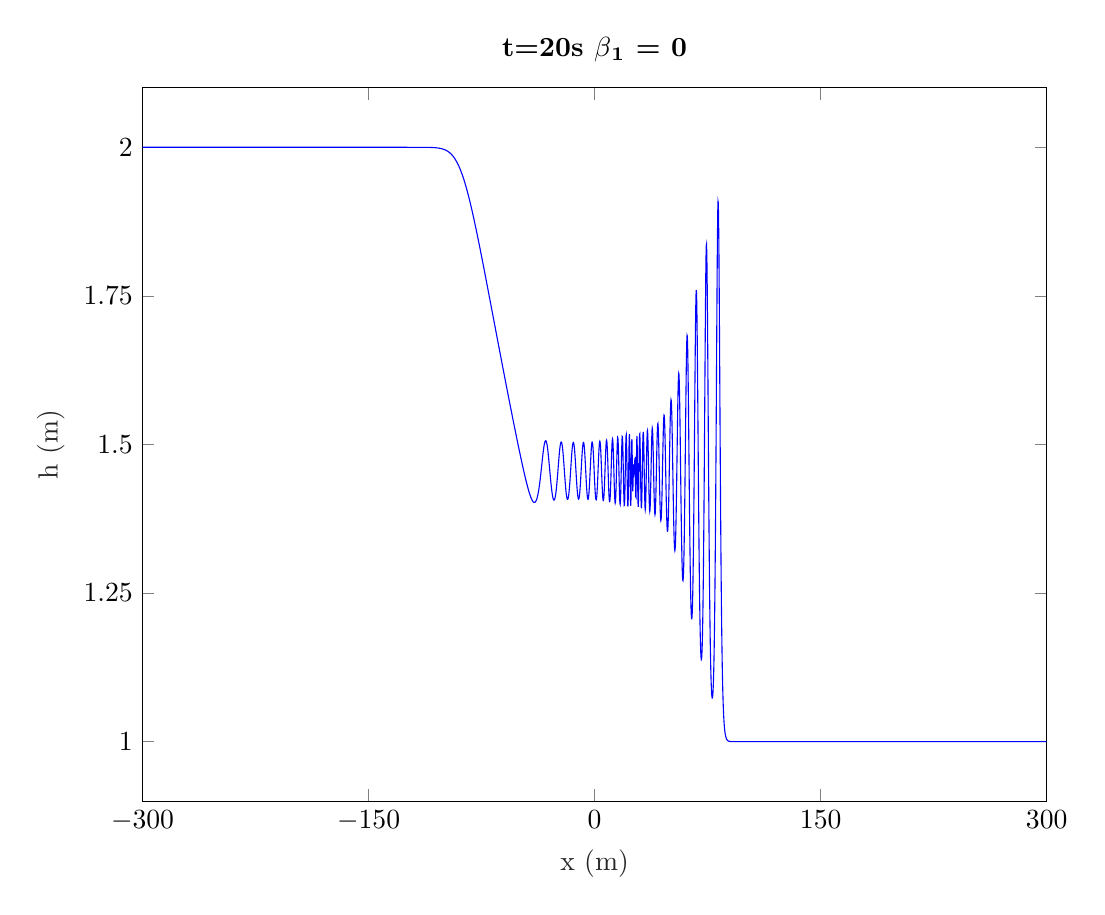
\begin{tikzpicture}

\begin{axis}[%
width=4.521in,
height=3.566in,
at={(0.758in,0.481in)},
scale only axis,
xmin=-300,
xmax=300,
xtick={-300, -150,    0,  150,  300},
xlabel style={font=\color{white!15!black}},
xlabel={x (m)},
ymin=0.9,
ymax=2.1,
ytick={   1, 1.25,  1.5, 1.75,    2},
ylabel style={font=\color{white!15!black}},
ylabel={h (m)},
axis background/.style={fill=white},
title style={font=\bfseries},
title={$\text{t=20s   }\beta{}_\text{1}\text{ = 0}$}
]
\addplot [color=blue, forget plot]
  table[row sep=crcr]{%
-300.18000900045	2\\
-300.030001500075	2\\
-299.8799939997	2\\
-299.729986499325	2\\
-299.57997899895	2\\
-299.429971498575	2\\
-299.2799639982	2\\
-299.129956497825	2\\
-298.97994899745	2\\
-298.829941497075	2\\
-298.6799339967	2\\
-298.529926496325	2\\
-298.37991899595	2\\
-298.229911495575	2\\
-298.0799039952	2\\
-297.929896494825	2\\
-297.77988899445	2\\
-297.629881494075	2\\
-297.4798739937	2\\
-297.329866493325	2\\
-297.17985899295	2\\
-297.029851492575	2\\
-296.8798439922	2\\
-296.729836491825	2\\
-296.57982899145	2\\
-296.429821491075	2\\
-296.2798139907	2\\
-296.129806490325	2\\
-295.979798989949	2\\
-295.829791489574	2\\
-295.679783989199	2\\
-295.529776488824	2\\
-295.379768988449	2\\
-295.229761488074	2\\
-295.079753987699	2\\
-294.929746487324	2\\
-294.779738986949	2\\
-294.629731486574	2\\
-294.479723986199	2\\
-294.329716485824	2\\
-294.179708985449	2\\
-294.029701485074	2\\
-293.879693984699	2\\
-293.729686484324	2\\
-293.579678983949	2\\
-293.429671483574	2\\
-293.279663983199	2\\
-293.129656482824	2\\
-292.979648982449	2\\
-292.829641482074	2\\
-292.679633981699	2\\
-292.529626481324	2\\
-292.379618980949	2\\
-292.229611480574	2\\
-292.079603980199	2\\
-291.929596479824	2\\
-291.779588979449	2\\
-291.629581479074	2\\
-291.479573978699	2\\
-291.329566478324	2\\
-291.179558977949	2\\
-291.029551477574	2\\
-290.879543977199	2\\
-290.729536476824	2\\
-290.579528976449	2\\
-290.429521476074	2\\
-290.279513975699	2\\
-290.129506475324	2\\
-289.979498974949	2\\
-289.829491474574	2\\
-289.679483974199	2\\
-289.529476473824	2\\
-289.379468973449	2\\
-289.229461473074	2\\
-289.079453972699	2\\
-288.929446472324	2\\
-288.779438971949	2\\
-288.629431471574	2\\
-288.479423971199	2\\
-288.329416470824	2\\
-288.179408970449	2\\
-288.029401470073	2\\
-287.879393969698	2\\
-287.729386469323	2\\
-287.579378968948	2\\
-287.429371468573	2\\
-287.279363968198	2\\
-287.129356467823	2\\
-286.979348967448	2\\
-286.829341467073	2\\
-286.679333966698	2\\
-286.529326466323	2\\
-286.379318965948	2\\
-286.229311465573	2\\
-286.079303965198	2\\
-285.929296464823	2\\
-285.779288964448	2\\
-285.629281464073	2\\
-285.479273963698	2\\
-285.329266463323	2\\
-285.179258962948	2\\
-285.029251462573	2\\
-284.879243962198	2\\
-284.729236461823	2\\
-284.579228961448	2\\
-284.429221461073	2\\
-284.279213960698	2\\
-284.129206460323	2\\
-283.979198959948	2\\
-283.829191459573	2\\
-283.679183959198	2\\
-283.529176458823	2\\
-283.379168958448	2\\
-283.229161458073	2\\
-283.079153957698	2\\
-282.929146457323	2\\
-282.779138956948	2\\
-282.629131456573	2\\
-282.479123956198	2\\
-282.329116455823	2\\
-282.179108955448	2\\
-282.029101455073	2\\
-281.879093954698	2\\
-281.729086454323	2\\
-281.579078953948	2\\
-281.429071453573	2\\
-281.279063953198	2\\
-281.129056452823	2\\
-280.979048952448	2\\
-280.829041452073	2\\
-280.679033951698	2\\
-280.529026451323	2\\
-280.379018950948	2\\
-280.229011450573	2\\
-280.079003950197	2\\
-279.928996449822	2\\
-279.778988949447	2\\
-279.628981449072	2\\
-279.478973948697	2\\
-279.328966448322	2\\
-279.178958947947	2\\
-279.028951447572	2\\
-278.878943947197	2\\
-278.728936446822	2\\
-278.578928946447	2\\
-278.428921446072	2\\
-278.278913945697	2\\
-278.128906445322	2\\
-277.978898944947	2\\
-277.828891444572	2\\
-277.678883944197	2\\
-277.528876443822	2\\
-277.378868943447	2\\
-277.228861443072	2\\
-277.078853942697	2\\
-276.928846442322	2\\
-276.778838941947	2\\
-276.628831441572	2\\
-276.478823941197	2\\
-276.328816440822	2\\
-276.178808940447	2\\
-276.028801440072	2\\
-275.878793939697	2\\
-275.728786439322	2\\
-275.578778938947	2\\
-275.428771438572	2\\
-275.278763938197	2\\
-275.128756437822	2\\
-274.978748937447	2\\
-274.828741437072	2\\
-274.678733936697	2\\
-274.528726436322	2\\
-274.378718935947	2\\
-274.228711435572	2\\
-274.078703935197	2\\
-273.928696434822	2\\
-273.778688934447	2\\
-273.628681434072	2\\
-273.478673933697	2\\
-273.328666433322	2\\
-273.178658932947	2\\
-273.028651432572	2\\
-272.878643932197	2\\
-272.728636431822	2\\
-272.578628931447	2\\
-272.428621431072	2\\
-272.278613930697	2\\
-272.128606430321	2\\
-271.978598929946	2\\
-271.828591429571	2\\
-271.678583929196	2\\
-271.528576428821	2\\
-271.378568928446	2\\
-271.228561428071	2\\
-271.078553927696	2\\
-270.928546427321	2\\
-270.778538926946	2\\
-270.628531426571	2\\
-270.478523926196	2\\
-270.328516425821	2\\
-270.178508925446	2\\
-270.028501425071	2\\
-269.878493924696	2\\
-269.728486424321	2\\
-269.578478923946	2\\
-269.428471423571	2\\
-269.278463923196	2\\
-269.128456422821	2\\
-268.978448922446	2\\
-268.828441422071	2\\
-268.678433921696	2\\
-268.528426421321	2\\
-268.378418920946	2\\
-268.228411420571	2\\
-268.078403920196	2\\
-267.928396419821	2\\
-267.778388919446	2\\
-267.628381419071	2\\
-267.478373918696	2\\
-267.328366418321	2\\
-267.178358917946	2\\
-267.028351417571	2\\
-266.878343917196	2\\
-266.728336416821	2\\
-266.578328916446	2\\
-266.428321416071	2\\
-266.278313915696	2\\
-266.128306415321	2\\
-265.978298914946	2\\
-265.828291414571	2\\
-265.678283914196	2\\
-265.528276413821	2\\
-265.378268913446	2\\
-265.228261413071	2\\
-265.078253912696	2\\
-264.928246412321	2\\
-264.778238911946	2\\
-264.628231411571	2\\
-264.478223911196	2\\
-264.328216410821	2\\
-264.178208910446	2\\
-264.02820141007	2\\
-263.878193909695	2\\
-263.72818640932	2\\
-263.578178908945	2\\
-263.42817140857	2\\
-263.278163908195	2\\
-263.12815640782	2\\
-262.978148907445	2\\
-262.82814140707	2\\
-262.678133906695	2\\
-262.52812640632	2\\
-262.378118905945	2\\
-262.22811140557	2\\
-262.078103905195	2\\
-261.92809640482	2\\
-261.778088904445	2\\
-261.62808140407	2\\
-261.478073903695	2\\
-261.32806640332	2\\
-261.178058902945	2\\
-261.02805140257	2\\
-260.878043902195	2\\
-260.72803640182	2\\
-260.578028901445	2\\
-260.42802140107	2\\
-260.278013900695	2\\
-260.12800640032	2\\
-259.977998899945	2\\
-259.82799139957	2\\
-259.677983899195	2\\
-259.52797639882	2\\
-259.377968898445	2\\
-259.22796139807	2\\
-259.077953897695	2\\
-258.92794639732	2\\
-258.777938896945	2\\
-258.62793139657	2\\
-258.477923896195	2\\
-258.32791639582	2\\
-258.177908895445	2\\
-258.02790139507	2\\
-257.877893894695	2\\
-257.72788639432	2\\
-257.577878893945	2\\
-257.42787139357	2\\
-257.277863893195	2\\
-257.12785639282	2\\
-256.977848892445	2\\
-256.82784139207	2\\
-256.677833891695	2\\
-256.52782639132	2\\
-256.377818890945	2\\
-256.22781139057	2\\
-256.077803890195	2\\
-255.927796389819	2\\
-255.777788889444	2\\
-255.627781389069	2\\
-255.477773888694	2\\
-255.327766388319	2\\
-255.177758887944	2\\
-255.027751387569	2\\
-254.877743887194	2\\
-254.727736386819	2\\
-254.577728886444	2\\
-254.427721386069	2\\
-254.277713885694	2\\
-254.127706385319	2\\
-253.977698884944	2\\
-253.827691384569	2\\
-253.677683884194	2\\
-253.527676383819	2\\
-253.377668883444	2\\
-253.227661383069	2\\
-253.077653882694	2\\
-252.927646382319	2\\
-252.777638881944	2\\
-252.627631381569	2\\
-252.477623881194	2\\
-252.327616380819	2\\
-252.177608880444	2\\
-252.027601380069	2\\
-251.877593879694	2\\
-251.727586379319	2\\
-251.577578878944	2\\
-251.427571378569	2\\
-251.277563878194	2\\
-251.127556377819	2\\
-250.977548877444	2\\
-250.827541377069	2\\
-250.677533876694	2\\
-250.527526376319	2\\
-250.377518875944	2\\
-250.227511375569	2\\
-250.077503875194	2\\
-249.927496374819	2\\
-249.777488874444	2\\
-249.627481374069	2\\
-249.477473873694	2\\
-249.327466373319	2\\
-249.177458872944	2\\
-249.027451372569	2\\
-248.877443872194	2\\
-248.727436371819	2\\
-248.577428871444	2\\
-248.427421371069	2\\
-248.277413870694	2\\
-248.127406370319	2\\
-247.977398869943	2\\
-247.827391369568	2\\
-247.677383869193	2\\
-247.527376368818	2\\
-247.377368868443	2\\
-247.227361368068	2\\
-247.077353867693	2\\
-246.927346367318	2\\
-246.777338866943	2\\
-246.627331366568	2\\
-246.477323866193	2\\
-246.327316365818	2\\
-246.177308865443	2\\
-246.027301365068	2\\
-245.877293864693	2\\
-245.727286364318	2\\
-245.577278863943	2\\
-245.427271363568	2\\
-245.277263863193	2\\
-245.127256362818	2\\
-244.977248862443	2\\
-244.827241362068	2\\
-244.677233861693	2\\
-244.527226361318	2\\
-244.377218860943	2\\
-244.227211360568	2\\
-244.077203860193	2\\
-243.927196359818	2\\
-243.777188859443	2\\
-243.627181359068	2\\
-243.477173858693	2\\
-243.327166358318	2\\
-243.177158857943	2\\
-243.027151357568	2\\
-242.877143857193	2\\
-242.727136356818	2\\
-242.577128856443	2\\
-242.427121356068	2\\
-242.277113855693	2\\
-242.127106355318	2\\
-241.977098854943	2\\
-241.827091354568	2\\
-241.677083854193	2\\
-241.527076353818	2\\
-241.377068853443	2\\
-241.227061353068	2\\
-241.077053852693	2\\
-240.927046352318	2\\
-240.777038851943	2\\
-240.627031351568	2\\
-240.477023851193	2\\
-240.327016350818	2\\
-240.177008850443	2\\
-240.027001350068	2\\
-239.876993849692	2\\
-239.726986349317	2\\
-239.576978848942	2\\
-239.426971348567	2\\
-239.276963848192	2\\
-239.126956347817	2\\
-238.976948847442	2\\
-238.826941347067	2\\
-238.676933846692	2\\
-238.526926346317	2\\
-238.376918845942	2\\
-238.226911345567	2\\
-238.076903845192	2\\
-237.926896344817	2\\
-237.776888844442	2\\
-237.626881344067	2\\
-237.476873843692	2\\
-237.326866343317	2\\
-237.176858842942	2\\
-237.026851342567	2\\
-236.876843842192	2\\
-236.726836341817	2\\
-236.576828841442	2\\
-236.426821341067	2\\
-236.276813840692	2\\
-236.126806340317	2\\
-235.976798839942	2\\
-235.826791339567	2\\
-235.676783839192	2\\
-235.526776338817	2\\
-235.376768838442	2\\
-235.226761338067	2\\
-235.076753837692	2\\
-234.926746337317	2\\
-234.776738836942	2\\
-234.626731336567	2\\
-234.476723836192	2\\
-234.326716335817	2\\
-234.176708835442	2\\
-234.026701335067	2\\
-233.876693834692	2\\
-233.726686334317	2\\
-233.576678833942	2\\
-233.426671333567	2\\
-233.276663833192	2\\
-233.126656332817	2\\
-232.976648832442	2\\
-232.826641332067	2\\
-232.676633831692	2\\
-232.526626331317	2\\
-232.376618830942	2\\
-232.226611330567	2\\
-232.076603830192	2\\
-231.926596329817	2\\
-231.776588829441	2\\
-231.626581329066	2\\
-231.476573828691	2\\
-231.326566328316	2\\
-231.176558827941	2\\
-231.026551327566	2\\
-230.876543827191	2\\
-230.726536326816	2\\
-230.576528826441	2\\
-230.426521326066	2\\
-230.276513825691	2\\
-230.126506325316	2\\
-229.976498824941	2\\
-229.826491324566	2\\
-229.676483824191	2\\
-229.526476323816	2\\
-229.376468823441	2\\
-229.226461323066	2\\
-229.076453822691	2\\
-228.926446322316	2\\
-228.776438821941	2\\
-228.626431321566	2\\
-228.476423821191	2\\
-228.326416320816	2\\
-228.176408820441	2\\
-228.026401320066	2\\
-227.876393819691	2\\
-227.726386319316	2\\
-227.576378818941	2\\
-227.426371318566	2\\
-227.276363818191	2\\
-227.126356317816	2\\
-226.976348817441	2\\
-226.826341317066	2\\
-226.676333816691	2\\
-226.526326316316	2\\
-226.376318815941	2\\
-226.226311315566	2\\
-226.076303815191	2\\
-225.926296314816	2\\
-225.776288814441	2\\
-225.626281314066	2\\
-225.476273813691	2\\
-225.326266313316	2\\
-225.176258812941	2\\
-225.026251312566	2\\
-224.876243812191	2\\
-224.726236311816	2\\
-224.576228811441	2\\
-224.426221311066	2\\
-224.276213810691	2\\
-224.126206310316	2\\
-223.976198809941	2\\
-223.826191309565	2\\
-223.67618380919	2\\
-223.526176308815	2\\
-223.37616880844	2\\
-223.226161308065	2\\
-223.07615380769	2\\
-222.926146307315	2\\
-222.77613880694	2\\
-222.626131306565	2\\
-222.47612380619	2\\
-222.326116305815	2\\
-222.17610880544	2\\
-222.026101305065	2\\
-221.87609380469	2\\
-221.726086304315	2\\
-221.57607880394	2\\
-221.426071303565	2\\
-221.27606380319	2\\
-221.126056302815	2\\
-220.97604880244	2\\
-220.826041302065	2\\
-220.67603380169	2\\
-220.526026301315	2\\
-220.37601880094	2\\
-220.226011300565	2\\
-220.07600380019	2\\
-219.925996299815	2\\
-219.77598879944	2\\
-219.625981299065	2\\
-219.47597379869	2\\
-219.325966298315	2\\
-219.17595879794	2\\
-219.025951297565	2\\
-218.87594379719	2\\
-218.725936296815	2\\
-218.57592879644	2\\
-218.425921296065	2\\
-218.27591379569	2\\
-218.125906295315	2\\
-217.97589879494	2\\
-217.825891294565	2\\
-217.67588379419	2\\
-217.525876293815	2\\
-217.37586879344	2\\
-217.225861293065	2\\
-217.07585379269	2\\
-216.925846292315	2\\
-216.77583879194	2\\
-216.625831291565	2\\
-216.47582379119	2\\
-216.325816290815	2\\
-216.17580879044	2\\
-216.025801290065	2\\
-215.875793789689	2\\
-215.725786289314	2\\
-215.575778788939	2\\
-215.425771288564	2\\
-215.275763788189	2\\
-215.125756287814	2\\
-214.975748787439	2\\
-214.825741287064	2\\
-214.675733786689	2\\
-214.525726286314	2\\
-214.375718785939	2\\
-214.225711285564	2\\
-214.075703785189	2\\
-213.925696284814	2\\
-213.775688784439	2\\
-213.625681284064	2\\
-213.475673783689	2\\
-213.325666283314	2\\
-213.175658782939	2\\
-213.025651282564	2\\
-212.875643782189	2\\
-212.725636281814	2\\
-212.575628781439	2\\
-212.425621281064	2\\
-212.275613780689	2\\
-212.125606280314	2\\
-211.975598779939	2\\
-211.825591279564	2\\
-211.675583779189	2\\
-211.525576278814	2\\
-211.375568778439	2\\
-211.225561278064	2\\
-211.075553777689	2\\
-210.925546277314	2\\
-210.775538776939	2\\
-210.625531276564	2\\
-210.475523776189	2\\
-210.325516275814	2\\
-210.175508775439	2\\
-210.025501275064	2\\
-209.875493774689	2\\
-209.725486274314	2\\
-209.575478773939	2\\
-209.425471273564	2\\
-209.275463773189	2\\
-209.125456272814	2\\
-208.975448772439	2\\
-208.825441272064	2\\
-208.675433771689	2\\
-208.525426271314	2\\
-208.375418770939	2\\
-208.225411270564	2\\
-208.075403770189	2\\
-207.925396269813	2\\
-207.775388769438	2\\
-207.625381269063	2\\
-207.475373768688	2\\
-207.325366268313	2\\
-207.175358767938	2\\
-207.025351267563	2\\
-206.875343767188	2\\
-206.725336266813	2\\
-206.575328766438	2\\
-206.425321266063	2\\
-206.275313765688	2\\
-206.125306265313	2\\
-205.975298764938	2\\
-205.825291264563	2\\
-205.675283764188	2\\
-205.525276263813	2\\
-205.375268763438	2\\
-205.225261263063	2\\
-205.075253762688	2\\
-204.925246262313	2\\
-204.775238761938	2\\
-204.625231261563	2\\
-204.475223761188	2\\
-204.325216260813	2\\
-204.175208760438	2\\
-204.025201260063	2\\
-203.875193759688	2\\
-203.725186259313	2\\
-203.575178758938	2\\
-203.425171258563	2\\
-203.275163758188	2\\
-203.125156257813	2\\
-202.975148757438	2\\
-202.825141257063	2\\
-202.675133756688	2\\
-202.525126256313	2\\
-202.375118755938	2\\
-202.225111255563	2\\
-202.075103755188	2\\
-201.925096254813	2\\
-201.775088754438	2\\
-201.625081254063	2\\
-201.475073753688	2\\
-201.325066253313	2\\
-201.175058752938	2\\
-201.025051252563	2\\
-200.875043752188	2\\
-200.725036251813	2\\
-200.575028751438	2\\
-200.425021251063	2\\
-200.275013750688	2\\
-200.125006250313	2\\
-199.974998749937	2\\
-199.824991249562	2\\
-199.674983749187	2\\
-199.524976248812	2\\
-199.374968748437	2\\
-199.224961248062	2\\
-199.074953747687	2\\
-198.924946247312	2\\
-198.774938746937	2\\
-198.624931246562	2\\
-198.474923746187	2\\
-198.324916245812	2\\
-198.174908745437	2\\
-198.024901245062	2\\
-197.874893744687	2\\
-197.724886244312	2\\
-197.574878743937	2\\
-197.424871243562	2\\
-197.274863743187	2\\
-197.124856242812	2\\
-196.974848742437	2\\
-196.824841242062	2\\
-196.674833741687	2\\
-196.524826241312	2\\
-196.374818740937	2\\
-196.224811240562	2\\
-196.074803740187	2\\
-195.924796239812	2\\
-195.774788739437	2\\
-195.624781239062	2\\
-195.474773738687	2\\
-195.324766238312	2\\
-195.174758737937	2\\
-195.024751237562	2\\
-194.874743737187	2\\
-194.724736236812	2\\
-194.574728736437	2\\
-194.424721236062	2\\
-194.274713735687	2\\
-194.124706235312	2\\
-193.974698734937	2\\
-193.824691234562	2\\
-193.674683734187	2\\
-193.524676233812	2\\
-193.374668733437	2\\
-193.224661233062	2\\
-193.074653732687	2\\
-192.924646232312	2\\
-192.774638731937	2\\
-192.624631231562	2\\
-192.474623731187	2\\
-192.324616230812	2\\
-192.174608730437	2\\
-192.024601230062	2\\
-191.874593729686	2\\
-191.724586229311	2\\
-191.574578728936	2\\
-191.424571228561	2\\
-191.274563728186	2\\
-191.124556227811	2\\
-190.974548727436	2\\
-190.824541227061	2\\
-190.674533726686	2\\
-190.524526226311	2\\
-190.374518725936	2\\
-190.224511225561	2\\
-190.074503725186	2\\
-189.924496224811	2\\
-189.774488724436	2\\
-189.624481224061	2\\
-189.474473723686	2\\
-189.324466223311	2\\
-189.174458722936	2\\
-189.024451222561	2\\
-188.874443722186	2\\
-188.724436221811	2\\
-188.574428721436	2\\
-188.424421221061	2\\
-188.274413720686	2\\
-188.124406220311	2\\
-187.974398719936	2\\
-187.824391219561	2\\
-187.674383719186	2\\
-187.524376218811	2\\
-187.374368718436	2\\
-187.224361218061	2\\
-187.074353717686	2\\
-186.924346217311	2\\
-186.774338716936	2\\
-186.624331216561	2\\
-186.474323716186	2\\
-186.324316215811	2\\
-186.174308715436	2\\
-186.024301215061	2\\
-185.874293714686	2\\
-185.724286214311	2\\
-185.574278713936	2\\
-185.424271213561	2\\
-185.274263713186	2\\
-185.124256212811	2\\
-184.974248712436	2\\
-184.824241212061	2\\
-184.674233711686	2\\
-184.524226211311	2\\
-184.374218710936	2\\
-184.224211210561	2\\
-184.074203710186	2\\
-183.92419620981	2\\
-183.774188709435	2\\
-183.62418120906	2\\
-183.474173708685	2\\
-183.32416620831	2\\
-183.174158707935	2\\
-183.02415120756	2\\
-182.874143707185	2\\
-182.72413620681	2\\
-182.574128706435	2\\
-182.42412120606	2\\
-182.274113705685	2\\
-182.12410620531	2\\
-181.974098704935	2\\
-181.82409120456	2\\
-181.674083704185	2\\
-181.52407620381	2\\
-181.374068703435	2\\
-181.22406120306	2\\
-181.074053702685	2\\
-180.92404620231	2\\
-180.774038701935	2\\
-180.62403120156	2\\
-180.474023701185	2\\
-180.32401620081	2\\
-180.174008700435	2\\
-180.02400120006	2\\
-179.873993699685	2\\
-179.72398619931	2\\
-179.573978698935	2\\
-179.42397119856	2\\
-179.273963698185	2\\
-179.12395619781	2\\
-178.973948697435	2\\
-178.82394119706	2\\
-178.673933696685	2\\
-178.52392619631	2\\
-178.373918695935	2\\
-178.22391119556	2\\
-178.073903695185	2\\
-177.92389619481	2\\
-177.773888694435	2\\
-177.62388119406	2\\
-177.473873693685	2\\
-177.32386619331	2\\
-177.173858692935	2\\
-177.02385119256	2\\
-176.873843692185	2\\
-176.72383619181	2\\
-176.573828691435	2\\
-176.42382119106	2\\
-176.273813690685	2\\
-176.123806190309	2\\
-175.973798689934	2\\
-175.823791189559	2\\
-175.673783689184	2\\
-175.523776188809	2\\
-175.373768688434	2\\
-175.223761188059	2\\
-175.073753687684	2\\
-174.923746187309	2\\
-174.773738686934	2\\
-174.623731186559	2\\
-174.473723686184	2\\
-174.323716185809	2\\
-174.173708685434	2\\
-174.023701185059	2\\
-173.873693684684	2\\
-173.723686184309	2\\
-173.573678683934	2\\
-173.423671183559	2\\
-173.273663683184	2\\
-173.123656182809	2\\
-172.973648682434	2\\
-172.823641182059	2\\
-172.673633681684	2\\
-172.523626181309	2\\
-172.373618680934	2\\
-172.223611180559	2\\
-172.073603680184	2\\
-171.923596179809	2\\
-171.773588679434	2\\
-171.623581179059	2\\
-171.473573678684	2\\
-171.323566178309	2\\
-171.173558677934	2\\
-171.023551177559	2\\
-170.873543677184	2\\
-170.723536176809	2\\
-170.573528676434	2\\
-170.423521176059	2\\
-170.273513675684	2\\
-170.123506175309	2\\
-169.973498674934	2\\
-169.823491174559	2\\
-169.673483674184	2\\
-169.523476173809	2\\
-169.373468673434	2\\
-169.223461173059	2\\
-169.073453672684	2\\
-168.923446172309	2\\
-168.773438671934	2\\
-168.623431171559	2\\
-168.473423671184	2\\
-168.323416170809	2\\
-168.173408670434	2\\
-168.023401170058	2\\
-167.873393669683	2\\
-167.723386169308	2\\
-167.573378668933	2\\
-167.423371168558	2\\
-167.273363668183	2\\
-167.123356167808	2\\
-166.973348667433	2\\
-166.823341167058	2\\
-166.673333666683	2\\
-166.523326166308	2\\
-166.373318665933	2\\
-166.223311165558	2\\
-166.073303665183	2\\
-165.923296164808	2\\
-165.773288664433	2\\
-165.623281164058	2\\
-165.473273663683	2\\
-165.323266163308	2\\
-165.173258662933	2\\
-165.023251162558	2\\
-164.873243662183	2\\
-164.723236161808	2\\
-164.573228661433	2\\
-164.423221161058	2\\
-164.273213660683	2\\
-164.123206160308	2\\
-163.973198659933	2\\
-163.823191159558	2\\
-163.673183659183	2\\
-163.523176158808	2\\
-163.373168658433	2\\
-163.223161158058	2\\
-163.073153657683	2\\
-162.923146157308	2\\
-162.773138656933	2\\
-162.623131156558	2\\
-162.473123656183	2\\
-162.323116155808	1.99999999999999\\
-162.173108655433	1.99999999999999\\
-162.023101155058	1.99999999999999\\
-161.873093654683	1.99999999999999\\
-161.723086154308	1.99999999999999\\
-161.573078653933	1.99999999999998\\
-161.423071153558	1.99999999999998\\
-161.273063653183	1.99999999999998\\
-161.123056152808	1.99999999999998\\
-160.973048652433	1.99999999999997\\
-160.823041152058	1.99999999999997\\
-160.673033651683	1.99999999999996\\
-160.523026151308	1.99999999999996\\
-160.373018650933	1.99999999999996\\
-160.223011150558	1.99999999999995\\
-160.073003650182	1.99999999999995\\
-159.922996149807	1.99999999999994\\
-159.772988649432	1.99999999999994\\
-159.622981149057	1.99999999999993\\
-159.472973648682	1.99999999999992\\
-159.322966148307	1.99999999999992\\
-159.172958647932	1.99999999999991\\
-159.022951147557	1.9999999999999\\
-158.872943647182	1.99999999999989\\
-158.722936146807	1.99999999999988\\
-158.572928646432	1.99999999999987\\
-158.422921146057	1.99999999999986\\
-158.272913645682	1.99999999999985\\
-158.122906145307	1.99999999999983\\
-157.972898644932	1.99999999999982\\
-157.822891144557	1.9999999999998\\
-157.672883644182	1.99999999999979\\
-157.522876143807	1.99999999999977\\
-157.372868643432	1.99999999999975\\
-157.222861143057	1.99999999999973\\
-157.072853642682	1.99999999999971\\
-156.922846142307	1.99999999999968\\
-156.772838641932	1.99999999999966\\
-156.622831141557	1.99999999999963\\
-156.472823641182	1.9999999999996\\
-156.322816140807	1.99999999999957\\
-156.172808640432	1.99999999999953\\
-156.022801140057	1.9999999999995\\
-155.872793639682	1.99999999999945\\
-155.722786139307	1.99999999999941\\
-155.572778638932	1.99999999999936\\
-155.422771138557	1.99999999999931\\
-155.272763638182	1.99999999999926\\
-155.122756137807	1.9999999999992\\
-154.972748637432	1.99999999999914\\
-154.822741137057	1.99999999999907\\
-154.672733636682	1.999999999999\\
-154.522726136307	1.99999999999892\\
-154.372718635932	1.99999999999884\\
-154.222711135557	1.99999999999875\\
-154.072703635182	1.99999999999865\\
-153.922696134807	1.99999999999855\\
-153.772688634432	1.99999999999844\\
-153.622681134057	1.99999999999832\\
-153.472673633682	1.99999999999819\\
-153.322666133307	1.99999999999805\\
-153.172658632932	1.9999999999979\\
-153.022651132557	1.99999999999774\\
-152.872643632182	1.99999999999757\\
-152.722636131807	1.99999999999738\\
-152.572628631432	1.99999999999718\\
-152.422621131057	1.99999999999697\\
-152.272613630682	1.99999999999674\\
-152.122606130307	1.99999999999649\\
-151.972598629931	1.99999999999622\\
-151.822591129556	1.99999999999594\\
-151.672583629181	1.99999999999563\\
-151.522576128806	1.9999999999953\\
-151.372568628431	1.99999999999494\\
-151.222561128056	1.99999999999456\\
-151.072553627681	1.99999999999415\\
-150.922546127306	1.99999999999371\\
-150.772538626931	1.99999999999324\\
-150.622531126556	1.99999999999273\\
-150.472523626181	1.99999999999218\\
-150.322516125806	1.9999999999916\\
-150.172508625431	1.99999999999097\\
-150.022501125056	1.99999999999029\\
-149.872493624681	1.99999999998957\\
-149.722486124306	1.99999999998879\\
-149.572478623931	1.99999999998795\\
-149.422471123556	1.99999999998705\\
-149.272463623181	1.99999999998609\\
-149.122456122806	1.99999999998505\\
-148.972448622431	1.99999999998394\\
-148.822441122056	1.99999999998275\\
-148.672433621681	1.99999999998147\\
-148.522426121306	1.99999999998009\\
-148.372418620931	1.99999999997861\\
-148.222411120556	1.99999999997703\\
-148.072403620181	1.99999999997533\\
-147.922396119806	1.99999999997351\\
-147.772388619431	1.99999999997155\\
-147.622381119056	1.99999999996945\\
-147.472373618681	1.9999999999672\\
-147.322366118306	1.99999999996478\\
-147.172358617931	1.99999999996219\\
-147.022351117556	1.99999999995941\\
-146.872343617181	1.99999999995643\\
-146.722336116806	1.99999999995323\\
-146.572328616431	1.9999999999498\\
-146.422321116056	1.99999999994612\\
-146.272313615681	1.99999999994217\\
-146.122306115306	1.99999999993794\\
-145.972298614931	1.99999999993341\\
-145.822291114556	1.99999999992854\\
-145.672283614181	1.99999999992333\\
-145.522276113806	1.99999999991774\\
-145.372268613431	1.99999999991174\\
-145.222261113056	1.99999999990532\\
-145.072253612681	1.99999999989844\\
-144.922246112306	1.99999999989106\\
-144.772238611931	1.99999999988315\\
-144.622231111556	1.99999999987467\\
-144.472223611181	1.99999999986559\\
-144.322216110806	1.99999999985586\\
-144.172208610431	1.99999999984543\\
-144.022201110056	1.99999999983426\\
-143.87219360968	1.99999999982229\\
-143.722186109305	1.99999999980947\\
-143.57217860893	1.99999999979574\\
-143.422171108555	1.99999999978103\\
-143.27216360818	1.99999999976528\\
-143.122156107805	1.99999999974841\\
-142.97214860743	1.99999999973034\\
-142.822141107055	1.99999999971099\\
-142.67213360668	1.99999999969027\\
-142.522126106305	1.99999999966809\\
-142.37211860593	1.99999999964434\\
-142.222111105555	1.99999999961891\\
-142.07210360518	1.99999999959169\\
-141.922096104805	1.99999999956256\\
-141.77208860443	1.99999999953138\\
-141.622081104055	1.999999999498\\
-141.47207360368	1.99999999946228\\
-141.322066103305	1.99999999942405\\
-141.17205860293	1.99999999938315\\
-141.022051102555	1.99999999933938\\
-140.87204360218	1.99999999929255\\
-140.722036101805	1.99999999924245\\
-140.57202860143	1.99999999918885\\
-140.422021101055	1.99999999913151\\
-140.27201360068	1.99999999907018\\
-140.122006100305	1.99999999900459\\
-139.97199859993	1.99999999893443\\
-139.821991099555	1.99999999885941\\
-139.67198359918	1.99999999877917\\
-139.521976098805	1.99999999869338\\
-139.37196859843	1.99999999860166\\
-139.221961098055	1.99999999850358\\
-139.07195359768	1.99999999839874\\
-138.921946097305	1.99999999828666\\
-138.77193859693	1.99999999816685\\
-138.621931096555	1.9999999980388\\
-138.47192359618	1.99999999790194\\
-138.321916095805	1.99999999775568\\
-138.17190859543	1.99999999759937\\
-138.021901095055	1.99999999743236\\
-137.87189359468	1.99999999725391\\
-137.721886094305	1.99999999706325\\
-137.57187859393	1.99999999685956\\
-137.421871093555	1.99999999664197\\
-137.27186359318	1.99999999640954\\
-137.121856092805	1.99999999616129\\
-136.97184859243	1.99999999589615\\
-136.821841092055	1.99999999561299\\
-136.67183359168	1.99999999531062\\
-136.521826091305	1.99999999498774\\
-136.37181859093	1.999999994643\\
-136.221811090555	1.99999999427495\\
-136.07180359018	1.99999999388202\\
-135.921796089805	1.99999999346258\\
-135.771788589429	1.99999999301487\\
-135.621781089054	1.99999999253701\\
-135.471773588679	1.99999999202702\\
-135.321766088304	1.99999999148277\\
-135.171758587929	1.999999990902\\
-135.021751087554	1.99999999028231\\
-134.871743587179	1.99999998962115\\
-134.721736086804	1.99999998891579\\
-134.571728586429	1.99999998816333\\
-134.421721086054	1.99999998736068\\
-134.271713585679	1.99999998650457\\
-134.121706085304	1.9999999855915\\
-133.971698584929	1.99999998461776\\
-133.821691084554	1.99999998357938\\
-133.671683584179	1.99999998247218\\
-133.521676083804	1.99999998129167\\
-133.371668583429	1.9999999800331\\
-133.221661083054	1.99999997869142\\
-133.071653582679	1.99999997726123\\
-132.921646082304	1.99999997573684\\
-132.771638581929	1.99999997411215\\
-132.621631081554	1.9999999723807\\
-132.471623581179	1.99999997053562\\
-132.321616080804	1.99999996856961\\
-132.171608580429	1.9999999664749\\
-132.021601080054	1.99999996424326\\
-131.871593579679	1.99999996186592\\
-131.721586079304	1.99999995933357\\
-131.571578578929	1.99999995663631\\
-131.421571078554	1.99999995376365\\
-131.271563578179	1.99999995070441\\
-131.121556077804	1.99999994744674\\
-130.971548577429	1.99999994397806\\
-130.821541077054	1.999999940285\\
-130.671533576679	1.99999993635336\\
-130.521526076304	1.99999993216808\\
-130.371518575929	1.99999992771315\\
-130.221511075554	1.9999999229716\\
-130.071503575179	1.99999991792541\\
-129.921496074804	1.99999991255544\\
-129.771488574429	1.99999990684141\\
-129.621481074054	1.99999990076176\\
-129.471473573679	1.99999989429366\\
-129.321466073304	1.99999988741286\\
-129.171458572929	1.99999988009365\\
-129.021451072554	1.99999987230876\\
-128.871443572179	1.99999986402926\\
-128.721436071804	1.99999985522448\\
-128.571428571429	1.9999998458619\\
-128.421421071054	1.99999983590704\\
-128.271413570679	1.99999982532334\\
-128.121406070304	1.99999981407205\\
-127.971398569929	1.99999980211211\\
-127.821391069553	1.9999997894\\
-127.671383569178	1.99999977588959\\
-127.521376068803	1.99999976153201\\
-127.371368568428	1.99999974627548\\
-127.221361068053	1.99999973006516\\
-127.071353567678	1.99999971284296\\
-126.921346067303	1.99999969454734\\
-126.771338566928	1.99999967511313\\
-126.621331066553	1.99999965447134\\
-126.471323566178	1.99999963254891\\
-126.321316065803	1.99999960926849\\
-126.171308565428	1.99999958454821\\
-126.021301065053	1.99999955830141\\
-125.871293564678	1.99999953043638\\
-125.721286064303	1.99999950085606\\
-125.571278563928	1.99999946945776\\
-125.421271063553	1.99999943613284\\
-125.271263563178	1.99999940076637\\
-125.121256062803	1.99999936323678\\
-124.971248562428	1.99999932341549\\
-124.821241062053	1.99999928116655\\
-124.671233561678	1.99999923634617\\
-124.521226061303	1.99999918880236\\
-124.371218560928	1.99999913837444\\
-124.221211060553	1.99999908489254\\
-124.071203560178	1.99999902817716\\
-123.921196059803	1.99999896803859\\
-123.771188559428	1.99999890427637\\
-123.621181059053	1.99999883667872\\
-123.471173558678	1.9999987650219\\
-123.321166058303	1.9999986890696\\
-123.171158557928	1.99999860857221\\
-123.021151057553	1.99999852326617\\
-122.871143557178	1.99999843287316\\
-122.721136056803	1.99999833709935\\
-122.571128556428	1.99999823563456\\
-122.421121056053	1.99999812815138\\
-122.271113555678	1.99999801430429\\
-122.121106055303	1.99999789372865\\
-121.971098554928	1.99999776603974\\
-121.821091054553	1.99999763083169\\
-121.671083554178	1.99999748767635\\
-121.521076053803	1.99999733612215\\
-121.371068553428	1.99999717569285\\
-121.221061053053	1.99999700588631\\
-121.071053552678	1.99999682617308\\
-120.921046052303	1.99999663599504\\
-120.771038551928	1.99999643476392\\
-120.621031051553	1.99999622185972\\
-120.471023551178	1.99999599662909\\
-120.321016050803	1.99999575838367\\
-120.171008550428	1.99999550639827\\
-120.021001050052	1.99999523990901\\
-119.870993549677	1.99999495811135\\
-119.720986049302	1.99999466015808\\
-119.570978548927	1.99999434515716\\
-119.420971048552	1.99999401216945\\
-119.270963548177	1.99999366020639\\
-119.120956047802	1.99999328822753\\
-118.970948547427	1.99999289513798\\
-118.820941047052	1.99999247978569\\
-118.670933546677	1.99999204095866\\
-118.520926046302	1.999991577382\\
-118.370918545927	1.99999108771483\\
-118.220911045552	1.99999057054712\\
-118.070903545177	1.9999900243963\\
-117.920896044802	1.99998944770376\\
-117.770888544427	1.99998883883118\\
-117.620881044052	1.99998819605675\\
-117.470873543677	1.99998751757113\\
-117.320866043302	1.99998680147333\\
-117.170858542927	1.99998604576633\\
-117.020851042552	1.99998524835257\\
-116.870843542177	1.99998440702922\\
-116.720836041802	1.99998351948326\\
-116.570828541427	1.99998258328629\\
-116.420821041052	1.99998159588927\\
-116.270813540677	1.99998055461684\\
-116.120806040302	1.99997945666157\\
-115.970798539927	1.99997829907791\\
-115.820791039552	1.99997707877582\\
-115.670783539177	1.99997579251427\\
-115.520776038802	1.99997443689441\\
-115.370768538427	1.99997300835243\\
-115.220761038052	1.99997150315217\\
-115.070753537677	1.99996991737749\\
-114.920746037302	1.99996824692419\\
-114.770738536927	1.99996648749181\\
-114.620731036552	1.99996463457489\\
-114.470723536177	1.99996268345411\\
-114.320716035802	1.99996062918691\\
-114.170708535427	1.99995846659784\\
-114.020701035052	1.99995619026858\\
-113.870693534677	1.99995379452746\\
-113.720686034302	1.99995127343873\\
-113.570678533927	1.9999486207913\\
-113.420671033552	1.99994583008723\\
-113.270663533177	1.99994289452961\\
-113.120656032802	1.99993980701017\\
-112.970648532427	1.99993656009636\\
-112.820641032052	1.99993314601798\\
-112.670633531677	1.99992955665337\\
-112.520626031302	1.99992578351512\\
-112.370618530927	1.99992181773528\\
-112.220611030552	1.99991765005002\\
-112.070603530176	1.99991327078391\\
-111.920596029801	1.99990866983351\\
-111.770588529426	1.99990383665056\\
-111.620581029051	1.99989876022454\\
-111.470573528676	1.99989342906472\\
-111.320566028301	1.99988783118161\\
-111.170558527926	1.99988195406788\\
-111.020551027551	1.99987578467861\\
-110.870543527176	1.99986930941102\\
-110.720536026801	1.99986251408356\\
-110.570528526426	1.99985538391437\\
-110.420521026051	1.99984790349916\\
-110.270513525676	1.99984005678839\\
-110.120506025301	1.99983182706387\\
-109.970498524926	1.9998231969147\\
-109.820491024551	1.9998141482125\\
-109.670483524176	1.99980466208605\\
-109.520476023801	1.99979471889526\\
-109.370468523426	1.99978429820441\\
-109.220461023051	1.99977337875479\\
-109.070453522676	1.9997619384366\\
-108.920446022301	1.99974995426028\\
-108.770438521926	1.99973740232701\\
-108.620431021551	1.99972425779869\\
-108.470423521176	1.99971049486715\\
-108.320416020801	1.99969608672272\\
-108.170408520426	1.99968100552219\\
-108.020401020051	1.99966522235601\\
-107.870393519676	1.99964870721496\\
-107.720386019301	1.99963142895607\\
-107.570378518926	1.99961335526802\\
-107.420371018551	1.99959445263586\\
-107.270363518176	1.99957468630515\\
-107.120356017801	1.99955402024557\\
-106.970348517426	1.99953241711385\\
-106.820341017051	1.99950983821635\\
-106.670333516676	1.99948624347092\\
-106.520326016301	1.99946159136846\\
-106.370318515926	1.99943583893387\\
-106.220311015551	1.99940894168671\\
-106.070303515176	1.99938085360136\\
-105.920296014801	1.99935152706689\\
-105.770288514426	1.9993209128466\\
-105.620281014051	1.99928896003727\\
-105.470273513676	1.99925561602822\\
-105.320266013301	1.99922082646017\\
-105.170258512926	1.99918453518398\\
-105.020251012551	1.99914668421929\\
-104.870243512176	1.99910721371322\\
-104.720236011801	1.99906606189908\\
-104.570228511426	1.99902316505515\\
-104.420221011051	1.99897845746373\\
-104.270213510676	1.99893187137036\\
-104.120206010301	1.99888333694347\\
-103.970198509925	1.99883278223435\\
-103.82019100955	1.99878013313763\\
-103.670183509175	1.99872531335241\\
-103.5201760088	1.99866824434395\\
-103.370168508425	1.9986088453062\\
-103.22016100805	1.99854703312518\\
-103.070153507675	1.99848272234328\\
-102.9201460073	1.99841582512464\\
-102.770138506925	1.99834625122171\\
-102.62013100655	1.99827390794312\\
-102.470123506175	1.99819870012284\\
-102.3201160058	1.99812053009096\\
-102.170108505425	1.99803929764602\\
-102.02010100505	1.99795490002915\\
-101.870093504675	1.99786723190003\\
-101.7200860043	1.99777618531489\\
-101.570078503925	1.99768164970662\\
-101.42007100355	1.99758351186716\\
-101.270063503175	1.99748165593223\\
-101.1200560028	1.99737596336871\\
-100.970048502425	1.99726631296453\\
-100.82004100205	1.99715258082146\\
-100.670033501675	1.99703464035087\\
-100.5200260013	1.99691236227242\\
-100.370018500925	1.99678561461611\\
-100.22001100055	1.99665426272765\\
-100.070003500175	1.99651816927721\\
-99.9199959998	1.99637719427195\\
-99.769988499425	1.99623119507218\\
-99.6199809990499	1.99608002641145\\
-99.4699734986749	1.99592354042066\\
-99.3199659982999	1.99576158665629\\
-99.1699584979249	1.99559401213286\\
-99.0199509975499	1.99542066135983\\
-98.8699434971749	1.99524137638292\\
-98.7199359967998	1.99505599683005\\
-98.5699284964248	1.99486435996195\\
-98.4199209960498	1.99466630072758\\
-98.2699134956748	1.99446165182442\\
-98.1199059952998	1.99425024376368\\
-97.9698984949247	1.99403190494054\\
-97.8198909945497	1.99380646170951\\
-97.6698834941747	1.99357373846489\\
-97.5198759937997	1.9933335577264\\
-97.3698684934247	1.99308574023003\\
-97.2198609930497	1.99283010502416\\
-97.0698534926746	1.99256646957085\\
-96.9198459922996	1.99229464985245\\
-96.7698384919246	1.99201446048332\\
-96.6198309915496	1.99172571482689\\
-96.4698234911746	1.99142822511771\\
-96.3198159907996	1.99112180258875\\
-96.1698084904245	1.99080625760362\\
-96.0198009900495	1.99048139979378\\
-95.8697934896745	1.99014703820053\\
-95.7197859892995	1.98980298142183\\
-95.5697784889244	1.98944903776363\\
-95.4197709885494	1.98908501539563\\
-95.2697634881744	1.98871072251145\\
-95.1197559877994	1.98832596749274\\
-94.9697484874244	1.9879305590773\\
-94.8197409870494	1.98752430653094\\
-94.6697334866743	1.98710701982269\\
-94.5197259862993	1.98667850980338\\
-94.3697184859243	1.98623858838712\\
-94.2197109855493	1.98578706873548\\
-94.0697034851743	1.98532376544419\\
-93.9196959847992	1.98484849473186\\
-93.7696884844242	1.98436107463057\\
-93.6196809840492	1.98386132517791\\
-93.4696734836742	1.98334906861025\\
-93.3196659832992	1.98282412955669\\
-93.1696584829241	1.98228633523355\\
-93.0196509825491	1.98173551563891\\
-92.8696434821741	1.9811715037468\\
-92.7196359817991	1.98059413570077\\
-92.5696284814241	1.98000325100631\\
-92.4196209810491	1.97939869272183\\
-92.269613480674	1.97878030764776\\
-92.119605980299	1.97814794651331\\
-91.969598479924	1.9775014641606\\
-91.819590979549	1.97684071972566\\
-91.669583479174	1.97616557681588\\
-91.5195759787989	1.97547590368362\\
-91.3695684784239	1.97477157339543\\
-91.2195609780489	1.97405246399662\\
-91.0695534776739	1.97331845867065\\
-90.9195459772989	1.97256944589313\\
-90.7695384769239	1.97180531957985\\
-90.6195309765488	1.97102597922871\\
-90.4695234761738	1.97023133005494\\
-90.3195159757988	1.96942128311953\\
-90.1695084754238	1.96859575545036\\
-90.0195009750487	1.96775467015576\\
-89.8694934746737	1.96689795653035\\
-89.7194859742987	1.96602555015263\\
-89.5694784739237	1.96513739297431\\
-89.4194709735487	1.96423343340102\\
-89.2694634731737	1.96331362636419\\
-89.1194559727986	1.96237793338399\\
-88.9694484724236	1.96142632262303\\
-88.8194409720486	1.96045876893085\\
-88.6694334716736	1.95947525387889\\
-88.5194259712986	1.95847576578603\\
-88.3694184709235	1.95746029973447\\
-88.2194109705485	1.95642885757602\\
-88.0694034701735	1.95538144792876\\
-87.9193959697985	1.95431808616398\\
-87.7693884694235	1.95323879438358\\
-87.6193809690484	1.95214360138792\\
-87.4693734686734	1.95103254263416\\
-87.3193659682984	1.94990566018531\\
-87.1693584679234	1.94876300264998\\
-87.0193509675484	1.94760462511312\\
-86.8693434671734	1.94643058905788\\
-86.7193359667984	1.94524096227881\\
-86.5693284664233	1.94403581878651\\
-86.4193209660483	1.94281523870423\\
-86.2693134656733	1.94157930815643\\
-86.1193059652983	1.94032811914973\\
-85.9692984649232	1.93906176944648\\
-85.8192909645482	1.93778036243145\\
-85.6692834641732	1.93648400697159\\
-85.5192759637982	1.93517281726975\\
-85.3692684634232	1.93384691271217\\
-85.2192609630482	1.9325064177106\\
-85.0692534626731	1.93115146153903\\
-84.9192459622981	1.92978217816578\\
-84.7692384619231	1.92839870608103\\
-84.6192309615481	1.92700118812044\\
-84.4692234611731	1.92558977128522\\
-84.319215960798	1.92416460655887\\
-84.169208460423	1.92272584872136\\
-84.019200960048	1.92127365616079\\
-83.869193459673	1.91980819068327\\
-83.719185959298	1.91832961732117\\
-83.5691784589229	1.91683810414038\\
-83.4191709585479	1.91533382204672\\
-83.2691634581729	1.9138169445922\\
-83.1191559577979	1.91228764778127\\
-82.9691484574229	1.91074610987753\\
-82.8191409570479	1.90919251121131\\
-82.6691334566728	1.90762703398844\\
-82.5191259562978	1.90604986210051\\
-82.3691184559228	1.90446118093709\\
-82.2191109555478	1.90286117720005\\
-82.0691034551728	1.90125003872049\\
-81.9190959547977	1.89962795427834\\
-81.7690884544227	1.89799511342516\\
-81.6190809540477	1.89635170631024\\
-81.4690734536727	1.89469792351024\\
-81.3190659532977	1.89303395586269\\
-81.1690584529227	1.89135999430354\\
-81.0190509525476	1.88967622970888\\
-80.8690434521726	1.88798285274116\\
-80.7190359517976	1.88628005369985\\
-80.5690284514226	1.884568022377\\
-80.4190209510475	1.88284694791746\\
-80.2690134506725	1.88111701868422\\
-80.1190059502975	1.87937842212876\\
-79.9689984499225	1.8776313446665\\
-79.8189909495475	1.87587597155754\\
-79.6689834491725	1.87411248679264\\
-79.5189759487974	1.87234107298445\\
-79.3689684484224	1.87056191126418\\
-79.2189609480474	1.86877518118345\\
-79.0689534476724	1.86698106062161\\
-78.9189459472974	1.86517972569826\\
-78.7689384469223	1.86337135069113\\
-78.6189309465473	1.86155610795912\\
-78.4689234461723	1.85973416787059\\
-78.3189159457973	1.85790569873676\\
-78.1689084454223	1.85607086675009\\
-78.0189009450472	1.85422983592772\\
-77.8688934446722	1.85238276805973\\
-77.7188859442972	1.85052982266215\\
-77.5688784439222	1.84867115693476\\
-77.4188709435472	1.84680692572326\\
-77.2688634431722	1.84493728148607\\
-77.1188559427972	1.84306237426533\\
-76.9688484424221	1.84118235166209\\
-76.8188409420471	1.83929735881567\\
-76.6688334416721	1.83740753838675\\
-76.5188259412971	1.83551303054444\\
-76.368818440922	1.83361397295686\\
-76.218810940547	1.83171050078529\\
-76.068803440172	1.82980274668161\\
-75.918795939797	1.827890840789\\
-75.768788439422	1.82597491074573\\
-75.618780939047	1.82405508169179\\
-75.4687734386719	1.82213147627835\\
-75.3187659382969	1.82020421467986\\
-75.1687584379219	1.81827341460858\\
-75.0187509375469	1.81633919133154\\
-74.8687434371719	1.81440165768963\\
-74.7187359367968	1.81246092411883\\
-74.5687284364218	1.81051709867333\\
-74.4187209360468	1.80857028705046\\
-74.2687134356718	1.80662059261732\\
-74.1187059352968	1.80466811643894\\
-73.9686984349217	1.80271295730789\\
-73.8186909345467	1.80075521177517\\
-73.6686834341717	1.79879497418233\\
-73.5186759337967	1.79683233669461\\
-73.3686684334217	1.79486738933513\\
-73.2186609330467	1.79290022001992\\
-73.0686534326716	1.79093091459368\\
-72.9186459322966	1.78895955686626\\
-72.7686384319216	1.78698622864974\\
-72.6186309315466	1.78501100979591\\
-72.4686234311716	1.78303397823427\\
-72.3186159307965	1.78105521001028\\
-72.1686084304215	1.77907477932393\\
-72.0186009300465	1.7770927585684\\
-71.8685934296715	1.77510921836889\\
-71.7185859292965	1.77312422762154\\
-71.5685784289215	1.77113785353223\\
-71.4185709285464	1.76915016165538\\
-71.2685634281714	1.76716121593264\\
-71.1185559277964	1.76517107873135\\
-70.9685484274214	1.76317981088281\\
-70.8185409270463	1.7611874717203\\
-70.6685334266713	1.7591941191168\\
-70.5185259262963	1.75719980952231\\
-70.3685184259213	1.75520459800087\\
-70.2185109255463	1.75320853826717\\
-70.0685034251713	1.75121168272268\\
-69.9184959247962	1.74921408249135\\
-69.7684884244212	1.74721578745488\\
-69.6184809240462	1.74521684628742\\
-69.4684734236712	1.74321730648977\\
-69.3184659232962	1.74121721442312\\
-69.1684584229211	1.73921661534215\\
-69.0184509225461	1.73721555342763\\
-68.8684434221711	1.73521407181848\\
-68.7184359217961	1.73321221264319\\
-68.5684284214211	1.73121001705077\\
-68.418420921046	1.72920752524099\\
-68.268413420671	1.72720477649417\\
-68.118405920296	1.72520180920032\\
-67.968398419921	1.72319866088773\\
-67.818390919546	1.72119536825097\\
-67.668383419171	1.7191919671783\\
-67.518375918796	1.71718849277861\\
-67.3683684184209	1.71518497940766\\
-67.2183609180459	1.71318146069386\\
-67.0683534176709	1.71117796956352\\
-66.9183459172959	1.70917453826546\\
-66.7683384169208	1.70717119839522\\
-66.6183309165458	1.70516798091869\\
-66.4683234161708	1.70316491619521\\
-66.3183159157958	1.70116203400023\\
-66.1683084154208	1.69915936354749\\
-66.0183009150458	1.69715693351067\\
-65.8682934146707	1.69515477204468\\
-65.7182859142957	1.6931529068064\\
-65.5682784139207	1.6911513649751\\
-65.4182709135457	1.68915017327239\\
-65.2682634131707	1.68714935798177\\
-65.1182559127956	1.68514894496785\\
-64.9682484124206	1.68314895969511\\
-64.8182409120456	1.68114942724646\\
-64.6682334116706	1.67915037234127\\
-64.5182259112956	1.67715181935329\\
-64.3682184109205	1.67515379232813\\
-64.2182109105455	1.67315631500047\\
-64.0682034101705	1.67115941081109\\
-63.9181959097955	1.66916310292356\\
-63.7681884094205	1.66716741424072\\
-63.6181809090455	1.66517236742101\\
-63.4681734086704	1.66317798489447\\
-63.3181659082954	1.66118428887876\\
-63.1681584079204	1.65919130139479\\
-63.0181509075454	1.65719904428239\\
-62.8681434071704	1.65520753921581\\
-62.7181359067953	1.65321680771902\\
-62.5681284064203	1.6512268711811\\
-62.4181209060453	1.64923775087139\\
-62.2681134056703	1.64724946795472\\
-62.1181059052953	1.64526204350659\\
-61.9680984049203	1.64327549852825\\
-61.8180909045452	1.64128985396197\\
-61.6680834041702	1.63930513070617\\
-61.5180759037952	1.63732134963074\\
-61.3680684034202	1.63533853159235\\
-61.2180609030451	1.63335669744997\\
-61.0680534026701	1.63137586808038\\
-60.9180459022951	1.62939606439393\\
-60.7680384019201	1.62741730735049\\
-60.6180309015451	1.62543961797547\\
-60.4680234011701	1.62346301737625\\
-60.318015900795	1.62148752675871\\
-60.16800840042	1.61951316744411\\
-60.018000900045	1.61753996088628\\
-59.86799339967	1.61556792868909\\
-59.717985899295	1.6135970926244\\
-59.5679783989199	1.61162747465029\\
-59.4179708985449	1.6096590969298\\
-59.2679633981699	1.60769198185009\\
-59.1179558977949	1.60572615204214\\
-58.9679483974199	1.60376163040098\\
-58.8179408970448	1.60179844010646\\
-58.6679333966698	1.5998366046447\\
-58.5179258962948	1.59787614783015\\
-58.3679183959198	1.59591709382837\\
-58.2179108955448	1.59395946717956\\
-58.0679033951698	1.59200329282291\\
-57.9178958947948	1.59004859612175\\
-57.7678883944197	1.58809540288963\\
-57.6178808940447	1.58614373941738\\
-57.4678733936697	1.58419363250112\\
-57.3178658932947	1.58224510947145\\
-57.1678583929196	1.58029819822364\\
-57.0178508925446	1.57835292724917\\
-56.8678433921696	1.57640932566848\\
-56.7178358917946	1.57446742326507\\
-56.5678283914196	1.57252725052105\\
-56.4178208910446	1.57058883865425\\
-56.2678133906695	1.56865221965688\\
-56.1178058902945	1.5667174263359\\
-55.9677983899195	1.56478449235526\\
-55.8177908895445	1.56285345227995\\
-55.6677833891695	1.56092434162215\\
-55.5177758887944	1.55899719688944\\
-55.3677683884194	1.55707205563532\\
-55.2177608880444	1.55514895651214\\
-55.0677533876694	1.55322793932646\\
-54.9177458872944	1.55130904509717\\
-54.7677383869193	1.54939231611643\\
-54.6177308865443	1.54747779601353\\
-54.4677233861693	1.54556552982204\\
-54.3177158857943	1.54365556405018\\
-54.1677083854193	1.54174794675482\\
-54.0177008850443	1.53984272761922\\
-53.8676933846692	1.53793995803473\\
-53.7176858842942	1.53603969118667\\
-53.5676783839192	1.53414198214476\\
-53.4176708835442	1.53224688795813\\
-53.2676633831692	1.53035446775547\\
-53.1176558827941	1.52846478285035\\
-52.9676483824191	1.5265778968522\\
-52.8176408820441	1.52469387578323\\
-52.6676333816691	1.52281278820166\\
-52.5176258812941	1.52093470533155\\
-52.3676183809191	1.51905970119977\\
-52.217610880544	1.51718785278039\\
-52.067603380169	1.5153192401471\\
-51.917595879794	1.51345394663395\\
-51.767588379419	1.51159205900511\\
-51.6175808790439	1.50973366763396\\
-51.4675733786689	1.5078788666924\\
-51.3175658782939	1.50602775435063\\
-51.1675583779189	1.50418043298833\\
-51.0175508775439	1.50233700941778\\
-50.8675433771689	1.50049759511966\\
-50.7175358767938	1.49866230649237\\
-50.5675283764188	1.49683126511564\\
-50.4175208760438	1.49500459802927\\
-50.2675133756688	1.49318243802801\\
-50.1175058752938	1.49136492397352\\
-49.9674983749187	1.48955220112439\\
-49.8174908745437	1.48774442148543\\
-49.6674833741687	1.48594174417737\\
-49.5174758737937	1.48414433582813\\
-49.3674683734187	1.48235237098708\\
-49.2174608730436	1.48056603256368\\
-49.0674533726686	1.47878551229181\\
-48.9174458722936	1.47701101122165\\
-48.7674383719186	1.47524274024044\\
-48.6174308715436	1.47348092062407\\
-48.4674233711686	1.47172578462128\\
-48.3174158707936	1.46997757607241\\
-48.1674083704185	1.46823655106477\\
-48.0174008700435	1.46650297862669\\
-47.8673933696685	1.46477714146272\\
-47.7173858692935	1.46305933673211\\
-47.5673783689184	1.46134987687333\\
-47.4173708685434	1.45964909047705\\
-47.2673633681684	1.45795732321042\\
-47.1173558677934	1.4562749387955\\
-46.9673483674184	1.45460232004487\\
-46.8173408670434	1.45293986995741\\
-46.6673333666683	1.45128801287766\\
-46.5173258662933	1.44964719572185\\
-46.3673183659183	1.44801788927428\\
-46.2173108655433	1.44640058955743\\
-46.0673033651683	1.44479581927951\\
-45.9172958647932	1.44320412936293\\
-45.7672883644182	1.44162610055773\\
-45.6172808640432	1.44006234514339\\
-45.4672733636682	1.43851350872293\\
-45.3172658632932	1.4369802721129\\
-45.1672583629181	1.43546335333283\\
-45.0172508625431	1.43396350969762\\
-44.8672433621681	1.43248154001606\\
-44.7172358617931	1.4310182868983\\
-44.5672283614181	1.42957463917506\\
-44.4172208610431	1.4281515344304\\
-44.267213360668	1.42674996164981\\
-44.117205860293	1.42537096398415\\
-43.967198359918	1.4240156416295\\
-43.817190859543	1.42268515482175\\
-43.667183359168	1.4213807269434\\
-43.5171758587929	1.42010364773878\\
-43.3671683584179	1.41885527663201\\
-43.2171608580429	1.41763704613991\\
-43.0671533576679	1.41645046536981\\
-42.9171458572928	1.41529712358936\\
-42.7671383569178	1.41417869385232\\
-42.6171308565428	1.41309693666043\\
-42.4671233561678	1.41205370363754\\
-42.3171158557928	1.41105094118711\\
-42.1671083554178	1.41009069409907\\
-42.0171008550428	1.40917510906533\\
-41.8670933546678	1.40830643805699\\
-41.7170858542927	1.40748704150789\\
-41.5670783539177	1.40671939124068\\
-41.4170708535427	1.40600607306202\\
-41.2670633531677	1.40534978894252\\
-41.1170558527926	1.4047533586853\\
-40.9670483524176	1.40421972097418\\
-40.8170408520426	1.40375193367809\\
-40.6670333516676	1.40335317327332\\
-40.5170258512925	1.40302673322846\\
-40.3670183509175	1.40277602117937\\
-40.2170108505425	1.40260455474939\\
-40.0670033501675	1.4025158562738\\
-39.9169958497925	1.40251420700323\\
-39.7669883494175	1.40260232490827\\
-39.6169808490425	1.40278497187187\\
-39.4669733486674	1.40306582793428\\
-39.3169658482924	1.4034488710947\\
-39.1669583479174	1.40393810830618\\
-39.0169508475424	1.40453753200058\\
-38.8669433471674	1.40525111364284\\
-38.7169358467924	1.40608274938629\\
-38.5669283464173	1.4070362390502\\
-38.4169208460423	1.40811523516245\\
-38.2669133456673	1.40932319344422\\
-38.1169058452923	1.41066333078661\\
-37.9668983449172	1.41213854669977\\
-37.8168908445422	1.41375138198276\\
-37.6668833441672	1.41550392356083\\
-37.5168758437922	1.41739774742892\\
-37.3668683434172	1.41943382334104\\
-37.2168608430421	1.42161243039849\\
-37.0668533426671	1.42393306995945\\
-36.9168458422921	1.42639435496685\\
-36.7668383419171	1.42899393093575\\
-36.6168308415421	1.43172835088895\\
-36.4668233411671	1.43459299833779\\
-36.3168158407921	1.43758196828617\\
-36.166808340417	1.44068798713957\\
-36.016800840042	1.44390231777131\\
-35.866793339667	1.44721468391953\\
-35.716785839292	1.45061320853529\\
-35.5667783389169	1.45408436218114\\
-35.4167708385419	1.45761293940427\\
-35.2667633381669	1.46118205496201\\
-35.1167558377919	1.46477316470044\\
-34.9667483374168	1.46836612916725\\
-34.8167408370418	1.47193929103245\\
-34.6667333366668	1.47546961573236\\
-34.5167258362918	1.47893284098844\\
-34.3667183359168	1.48230369396635\\
-34.2167108355418	1.4855561241428\\
-34.0667033351668	1.48866358968792\\
-33.9166958347918	1.49159937167523\\
-33.7666883344167	1.49433691812537\\
-33.6166808340417	1.4968502200361\\
-33.4666733336667	1.49911419589617\\
-33.3166658332917	1.50110509514881\\
-33.1666583329167	1.50280089680238\\
-33.0166508325416	1.50418169869095\\
-32.8666433321666	1.50523009239723\\
-32.7166358317916	1.50593149839217\\
-32.5666283314166	1.50627611597674\\
-32.4166208310415	1.50625025354612\\
-32.2666133306665	1.50585637322851\\
-32.1166058302915	1.50509007038832\\
-31.9665983299165	1.50395502605792\\
-31.8165908295415	1.50245795338461\\
-31.6665833291665	1.50060929494298\\
-31.5165758287914	1.49842305952556\\
-31.3665683284164	1.4959165512994\\
-31.2165608280414	1.49311018882686\\
-31.0665533276664	1.49002715334439\\
-30.9165458272914	1.48669304540822\\
-30.7665383269164	1.48313556253315\\
-30.6165308265414	1.47938403490081\\
-30.4665233261663	1.47546908051411\\
-30.3165158257913	1.47142225484945\\
-30.1665083254163	1.46727556481453\\
-30.0165008250412	1.46306120468344\\
-29.8664933246662	1.4588112440658\\
-29.7164858242912	1.45455722349066\\
-29.5664783239162	1.45033000747241\\
-29.4164708235412	1.44615954012955\\
-29.2664633231661	1.44207460138502\\
-29.1164558227911	1.43810274782631\\
-28.9664483224161	1.43427016182908\\
-28.8164408220411	1.43060157630701\\
-28.6664333216661	1.4271202479606\\
-28.5164258212911	1.42384792057725\\
-28.3664183209161	1.42080485267384\\
-28.216410820541	1.41800978859833\\
-28.066403320166	1.41548002729454\\
-27.916395819791	1.41323145142597\\
-27.766388319416	1.41127850464614\\
-27.616380819041	1.40963430003568\\
-27.4663733186659	1.40831058260998\\
-27.3163658182909	1.40731772635634\\
-27.1663583179159	1.40666478218632\\
-27.0163508175409	1.40635735116408\\
-26.8663433171658	1.40640819496165\\
-26.7163358167908	1.40681444549949\\
-26.5663283164158	1.40758254423396\\
-26.4163208160408	1.4087132773778\\
-26.2663133156658	1.41020596279624\\
-26.1163058152908	1.41205778875481\\
-25.9662983149157	1.41426361764759\\
-25.8162908145407	1.41681576450842\\
-25.6662833141657	1.41970373063184\\
-25.5162758137907	1.42291398408879\\
-25.3662683134157	1.42642969497965\\
-25.2162608130407	1.4302304915134\\
-25.0662533126657	1.43429227863109\\
-24.9162458122906	1.43858702296048\\
-24.7662383119156	1.44308266133754\\
-24.6162308115406	1.44774302960488\\
-24.4662233111655	1.45252788880842\\
-24.3162158107905	1.45739306153882\\
-24.1662083104155	1.46229065684381\\
-24.0162008100405	1.46716944958379\\
-23.8661933096655	1.47197536420971\\
-23.7161858092904	1.47665211977513\\
-23.5661783089154	1.48114200127327\\
-23.4161708085404	1.48538675350815\\
-23.2661633081654	1.48932860496712\\
-23.1161558077904	1.49291136803691\\
-22.9661483074154	1.49608161400671\\
-22.8161408070404	1.49878986294673\\
-22.6661333066654	1.50099177351966\\
-22.5161258062903	1.50264926872883\\
-22.3661183059153	1.50373156892888\\
-22.2161108055403	1.50422180388881\\
-22.0661033051653	1.50408831262851\\
-21.9160958047902	1.50334579655819\\
-21.7660883044152	1.50199208169142\\
-21.6160808040402	1.50004256719378\\
-21.4660733036652	1.49752151624836\\
-21.3160658032901	1.49446207978646\\
-21.1660583029151	1.4909056308074\\
-21.0160508025401	1.48690087279764\\
-20.8660433021651	1.48250281265529\\
-20.7160358017901	1.47777164176366\\
-20.5660283014151	1.47277153457726\\
-20.4160208010401	1.46756947310968\\
-20.266013300665	1.46223402128222\\
-20.11600580029	1.45683426842989\\
-19.965998299915	1.45143873642217\\
-19.81599079954	1.44611451292267\\
-19.665983299165	1.44092641246196\\
-19.51597579879	1.43593633050222\\
-19.3659682984149	1.4312026897385\\
-19.2159607980399	1.42678001368233\\
-19.0659532976649	1.42271860639743\\
-18.9159457972899	1.41906431740405\\
-18.7659382969148	1.41585838296492\\
-18.6159307965398	1.41313730396524\\
-18.4659232961648	1.41093276254978\\
-18.3159157957898	1.40927154039798\\
-18.1659082954148	1.40817542868031\\
-18.0159007950397	1.40765744533598\\
-17.8658932946647	1.40774097156605\\
-17.7158857942897	1.40841820012229\\
-17.5658782939147	1.40969571776623\\
-17.4158707935397	1.41156679671345\\
-17.2658632931647	1.41401931488453\\
-17.1158557927897	1.41703426757328\\
-16.9658482924146	1.42058556579908\\
-16.8158407920396	1.42463950480444\\
-16.6658332916646	1.42915450960917\\
-16.5158257912896	1.43408081792769\\
-16.3658182909145	1.43936035405423\\
-16.2158107905395	1.44492673978432\\
-16.0658032901645	1.45070554567641\\
-15.9157957897895	1.45661475706049\\
-15.7657882894144	1.46256559471997\\
-15.6157807890394	1.46846358267366\\
-15.4657732886644	1.47421005189286\\
-15.3157657882894	1.47970388866666\\
-15.1657582879144	1.48484366418234\\
-15.0157507875394	1.48952999185873\\
-14.8657432871644	1.4936681058516\\
-14.7157357867894	1.49717052615941\\
-14.5657282864143	1.49995971057821\\
-14.4157207860393	1.5019705987119\\
-14.2657132856643	1.50315259952869\\
-14.1157057852893	1.50346734710365\\
-13.9656982849143	1.50291451240925\\
-13.8156907845392	1.50148161950826\\
-13.6656832841642	1.49919608305636\\
-13.5156757837892	1.49609875061432\\
-13.3656682834142	1.492247994627\\
-13.2156607830391	1.48771812213467\\
-13.0656532826641	1.48259732631793\\
-12.9156457822891	1.47698528166532\\
-12.7656382819141	1.47099052296635\\
-12.6156307815391	1.46472762961208\\
-12.4656232811641	1.45831458165095\\
-12.315615780789	1.45187019160358\\
-12.165608280414	1.44551166597621\\
-12.015600780039	1.43935248121572\\
-11.865593279664	1.43350066829634\\
-11.715585779289	1.42805727181664\\
-11.565578278914	1.42311507228726\\
-11.4155707785389	1.41875771938591\\
-11.2655632781639	1.41505902717394\\
-11.1155557777889	1.41208231194128\\
-10.9655482774139	1.40988000860605\\
-10.8155407770388	1.40849325427782\\
-10.6655332766638	1.40794535149807\\
-10.5155257762888	1.408272645746\\
-10.3655182759138	1.40946024623627\\
-10.2155107755388	1.41150688673307\\
-10.0655032751637	1.41439028081748\\
-9.91549577478872	1.41807411578516\\
-9.76548827441371	1.42250723010076\\
-9.6154807740387	1.42762309775937\\
-9.46547327366369	1.43333962718576\\
-9.31546577328868	1.43955911476523\\
-9.16545827291367	1.44616869992127\\
-9.0154507725386	1.4530412844471\\
-8.86544327216359	1.46003708885914\\
-8.71543577178858	1.46700590297997\\
-8.56542827141357	1.47379007887905\\
-8.41542077103855	1.48022825371905\\
-8.26541327066354	1.48615974185548\\
-8.11540577028853	1.49142947752266\\
-7.96539826991352	1.49589328016418\\
-7.81539076953845	1.49942322795546\\
-7.66538326916344	1.50191278678383\\
-7.51537576878843	1.50328117548167\\
-7.36536826841342	1.5034709327895\\
-7.21536076803841	1.50248518145997\\
-7.0653532676634	1.50031783389262\\
-6.91534576728839	1.49702554717658\\
-6.76533826691332	1.49268990438022\\
-6.61533076653831	1.48742204147961\\
-6.4653232661633	1.48135867584492\\
-6.31531576578828	1.47465734471678\\
-6.16530826541327	1.46749109691116\\
-6.01530076503826	1.46004293835954\\
-5.86529326466325	1.45250034242839\\
-5.71528576428824	1.44505006810464\\
-5.56527826391317	1.43787350285885\\
-5.41527076353816	1.43114260346197\\
-5.26526326316315	1.42501650890397\\
-5.11525576278814	1.41963880355772\\
-4.96524826241313	1.41513534521393\\
-4.81524076203812	1.41161255045247\\
-4.6652332616631	1.40915607692491\\
-4.51522576128809	1.40782972953698\\
-4.36521826091303	1.40768130129256\\
-4.21521076053801	1.40870708010057\\
-4.065203260163	1.4109197046736\\
-3.91519575978799	1.4142786052892\\
-3.76518825941298	1.41872328051811\\
-3.61518075903797	1.42416568739291\\
-3.46517325866296	1.43048985214023\\
-3.31516575828789	1.43755201942989\\
-3.16515825791288	1.4451816385593\\
-3.01515075753787	1.45318336794345\\
-2.86514325716286	1.46134043221821\\
-2.71513575678784	1.46941936715136\\
-2.56512825641283	1.47717642077651\\
-2.41512075603782	1.48436533515404\\
-2.26511325566281	1.49074639598266\\
-2.11510575528774	1.49609636094293\\
-1.96509825491273	1.500218691565\\
-1.81509075453772	1.50295337966343\\
-1.66508325416271	1.50420439183811\\
-1.5150757537877	1.50385022852289\\
-1.36506825341269	1.50194575142995\\
-1.21506075303768	1.49851958000574\\
-1.06505325266261	1.49368043823793\\
-0.915045752287597	1.48758786501733\\
-0.765038251912586	1.48044622464465\\
-0.615030751537574	1.47249583604516\\
-0.465023251162563	1.46400272496919\\
-0.315015750787552	1.45524805463654\\
-0.165008250412541	1.44651751701165\\
-0.0150007500375295	1.43809165511401\\
0.135006750337539	1.4302372399522\\
0.28501425071255	1.42319997940867\\
0.435021751087561	1.41719860683574\\
0.585029251462572	1.41242018076997\\
0.735036751837583	1.40901643445955\\
0.885044252212595	1.40710175766609\\
1.03505175258761	1.40675630057324\\
1.18505925296267	1.40798412998749\\
1.33506675333768	1.41079845820533\\
1.4850742537127	1.41512885591927\\
1.63508175408771	1.42086697656877\\
1.78508925446272	1.4278557653669\\
1.93509675483773	1.43589006627613\\
2.08510425521274	1.4447183409191\\
2.23511175558775	1.45404687123656\\
2.38511925596282	1.46354638349289\\
2.53512675633783	1.47286181958606\\
2.68513425671284	1.48162523405518\\
2.83514175708785	1.48947149386277\\
2.98514925746287	1.49605629887695\\
3.13515675783788	1.5010750865517\\
3.28516425821289	1.5042816737046\\
3.43517175858796	1.50551618561016\\
3.58517925896297	1.50465796159389\\
3.73518675933798	1.50175769434515\\
3.88519425971299	1.49690797072972\\
4.035201760088	1.49030910125979\\
4.18520926046301	1.48224168556938\\
4.33521676083802	1.47305207683468\\
4.48522426121303	1.46313393836058\\
4.6352317615881	1.45290820062783\\
4.78523926196311	1.44280321872259\\
4.93524676233812	1.4332363645729\\
5.08525426271314	1.42459777702142\\
5.23526176308815	1.41723709246708\\
5.38526926346316	1.41145279636098\\
5.53527676383817	1.40748386186864\\
5.68528426421324	1.40549157183283\\
5.83529176458825	1.4056205400236\\
5.98529926496326	1.40784264878794\\
6.13530676533827	1.41213661335003\\
6.28531426571328	1.41836262665652\\
6.43532176608829	1.42630409058352\\
6.5853292664633	1.43566171765377\\
6.73533676683832	1.44605752932934\\
6.88534426721338	1.45704320284588\\
7.03535176758839	1.46811407330935\\
7.18535926796341	1.47872949364407\\
7.33536676833842	1.48833953400383\\
7.48537426871343	1.49641691035111\\
7.63538176908844	1.50249215295124\\
7.78538926946345	1.50618695716896\\
7.93539676983852	1.5072334532487\\
8.08540427021353	1.50558012609656\\
8.23541177058854	1.50122838761467\\
8.38541927096355	1.49441108617328\\
8.53542677133856	1.48549144825858\\
8.68543427171358	1.47495462203881\\
8.83544177208859	1.46337572378652\\
8.9854492724636	1.4513826418119\\
9.13545677283867	1.43961818302987\\
9.28546427321368	1.428704934428\\
9.43547177358869	1.41921479049282\\
9.5854792739637	1.41164415762925\\
9.73548677433871	1.40639449121725\\
9.88549427471372	1.40373923712926\\
10.0355017750887	1.40391566917732\\
10.1855092754638	1.40687907375668\\
10.3355167758388	1.41258128837745\\
10.4855242762138	1.42077491929846\\
10.6355317765888	1.43107929876386\\
10.7855392769638	1.44297467990305\\
10.9355467773389	1.4558151486154\\
11.0855542777139	1.46885273189938\\
11.2355617780889	1.48127455352701\\
11.3855692784639	1.49225359945596\\
11.535576778839	1.50101034495787\\
11.685584279214	1.50688037845919\\
11.835591779589	1.50942437417774\\
11.985599279964	1.50824710050734\\
12.135606780339	1.50351745112901\\
12.285614280714	1.49546842217463\\
12.435621781089	1.48464697699083\\
12.5856292814641	1.47180456692854\\
12.7356367818391	1.45783724504363\\
12.8856442822141	1.44371349664261\\
13.0356517825891	1.4304021697201\\
13.1856592829641	1.41880791928162\\
13.3356667833391	1.40971751785821\\
13.4856742837142	1.40375826394366\\
13.6356817840892	1.40133171919419\\
13.7856892844642	1.40277276964315\\
13.9356967848393	1.40795175121203\\
14.0857042852143	1.41665954615041\\
14.2357117855893	1.42838759971663\\
14.3857192859643	1.44238258732136\\
14.5357267863393	1.45766617605721\\
14.6857342867143	1.4730813004925\\
14.8357417870894	1.48736781118855\\
14.9857492874644	1.49926746942437\\
15.1357567878394	1.50765145277255\\
15.2857642882144	1.5117411840291\\
15.4357717885894	1.51077130508047\\
15.5857792889644	1.50500181638321\\
15.7357867893394	1.49478460885445\\
15.8857942897145	1.48101833956078\\
16.0358017900895	1.46494482258245\\
16.1858092904645	1.44802033836777\\
16.3358167908395	1.43176896211736\\
16.4858242912146	1.4176436844791\\
16.6358317915896	1.40690882849565\\
16.7858392919646	1.40055362121137\\
16.9358467923396	1.39924678952301\\
17.0858542927147	1.4031068779463\\
17.2358617930897	1.41206474272494\\
17.3858692934647	1.42542611683583\\
17.5358767938397	1.44208154317485\\
17.6858842942147	1.460501189241\\
17.8358917945897	1.47882784663711\\
17.9858992949647	1.49504061500701\\
18.1359067953398	1.50718827481298\\
18.2859142957148	1.51375525151839\\
18.4359217960898	1.51342654604856\\
18.5859292964648	1.50643522237189\\
18.7359367968398	1.4932969218765\\
18.8859442972148	1.47557950076895\\
19.0359517975899	1.45542226874452\\
19.1859592979649	1.43527261011374\\
19.3359667983399	1.41757270437189\\
19.485974298715	1.40447869659161\\
19.63598179909	1.39754826485247\\
19.785989299465	1.39808172845281\\
19.93599679984	1.40588106636935\\
20.086004300215	1.42046550036483\\
20.23601180059	1.44021191306555\\
20.3860193009651	1.46267207876697\\
20.5360268013401	1.48472424401579\\
20.6860343017151	1.50294763621182\\
20.8360418020901	1.51419307742833\\
20.9860493024651	1.51608265436356\\
21.1360568028401	1.50823367758496\\
21.2860643032151	1.49138128914155\\
21.4360718035902	1.46841328843768\\
21.5860793039652	1.44319804415874\\
21.7360868043402	1.42012915819107\\
21.8860943047152	1.4032178172228\\
22.0361018050903	1.39544097991426\\
22.1861093054653	1.39906034389731\\
22.3361168058403	1.41335839230965\\
22.4861243062153	1.43655246038852\\
22.6361318065904	1.46447635368989\\
22.7861393069654	1.49139745650415\\
22.9361468073404	1.51085442550736\\
23.0861543077154	1.51732792934987\\
23.2361618080904	1.50851675078388\\
23.3861693084654	1.48571816491672\\
23.5361768088404	1.45482526709627\\
23.6861843092154	1.42421655382002\\
23.8361918095905	1.40257591409782\\
23.9861993099655	1.39694899193057\\
24.1362068103405	1.40973441642923\\
24.2862143107155	1.43883969393156\\
24.4362218110905	1.47494212587603\\
24.5862293114656	1.50389809123434\\
24.7362368118406	1.50910800697549\\
24.8862443122156	1.48979461992124\\
25.0362518125906	1.45582110922604\\
25.1862593129657	1.42754565395979\\
25.3362668133407	1.42102956967558\\
25.4862743137157	1.43442279665625\\
25.6362818140907	1.45530236930296\\
25.7862893144657	1.46658071574084\\
25.9362968148407	1.46420702087109\\
26.0863043152158	1.45624668748788\\
26.2363118155908	1.4517968188243\\
26.3863193159658	1.45416473325128\\
26.5363268163408	1.46491765374391\\
26.6863343167158	1.4761609194069\\
26.8363418170908	1.47670132840795\\
26.9863493174659	1.45879572178245\\
27.1363568178409	1.43163407940171\\
27.2863643182159	1.41200727892105\\
27.4363718185909	1.41114839694361\\
27.586379318966	1.43468243911255\\
27.736386819341	1.46954731247737\\
27.886394319716	1.50075020148485\\
28.036401820091	1.51458941438743\\
28.186409320466	1.50787012222374\\
28.3364168208411	1.48302409092081\\
28.4864243212161	1.45087135433644\\
28.6364318215911	1.42105884559713\\
28.7864393219661	1.40112102743519\\
28.9364468223411	1.39518141092434\\
29.0864543227161	1.40377219556874\\
29.2364618230911	1.42440241798184\\
29.3864693234661	1.45224214380336\\
29.5364768238412	1.48102715894407\\
29.6864843242162	1.50445701862941\\
29.8364918245912	1.51750637784502\\
29.9864993249662	1.51826841719956\\
30.1365068253413	1.50581126051889\\
30.2865143257163	1.48439229908601\\
30.4365218260913	1.4582229143482\\
30.5865293264663	1.43223571333771\\
30.7365368268414	1.41075804596301\\
30.8865443272164	1.39693306596973\\
31.0365518275914	1.39253301493925\\
31.1865593279664	1.39774198738628\\
31.3365668283414	1.41168062391271\\
31.4865743287164	1.43222133356507\\
31.6365818290914	1.45635230655699\\
31.7865893294665	1.48056525216119\\
31.9365968298415	1.50131524654116\\
32.0866043302165	1.51556793904354\\
32.2366118305915	1.52120500212748\\
32.3866193309665	1.51789691069366\\
32.5366268313416	1.50604609379004\\
32.6866343317166	1.48772409973556\\
32.8366418320916	1.46563185209007\\
32.9866493324666	1.44272252312536\\
33.1366568328417	1.42177953618228\\
33.2866643332167	1.40510300650662\\
33.4366718335917	1.3943439368601\\
33.5866793339667	1.3904961616455\\
33.7366868343417	1.39362182079076\\
33.8866943347167	1.40343833575844\\
34.0367018350918	1.41886173027124\\
34.1867093354668	1.43829882736925\\
34.3367168358418	1.4597528361545\\
34.4867243362168	1.48098000566676\\
34.6367318365918	1.49971366239567\\
34.7867393369668	1.51392599638683\\
34.9367468373418	1.52207912699735\\
35.0867543377169	1.52349275261482\\
35.2367618380919	1.51774313991345\\
35.3867693384669	1.5059518729379\\
35.5367768388419	1.48938231789447\\
35.686784339217	1.46982651261161\\
35.836791839592	1.44924005603892\\
35.986799339967	1.42952038187081\\
36.136806840342	1.41233716885056\\
36.2868143407171	1.39902462727094\\
36.4368218410921	1.39052855707905\\
36.5868293414671	1.38743472004593\\
36.7368368418421	1.3897641165936\\
36.8868443422171	1.39740048597502\\
37.0368518425921	1.40972834131959\\
37.1868593429671	1.42582132279853\\
37.3368668433422	1.44447252179109\\
37.4868743437172	1.46424955280448\\
37.6368818440922	1.48358603823608\\
37.7868893444672	1.50090294670043\\
37.9368968448422	1.51475151402332\\
38.0869043452172	1.5239596893898\\
38.2369118455923	1.52770350519431\\
38.3869193459673	1.52587268388096\\
38.5369268463423	1.51851426269874\\
38.6869343467174	1.50638542507259\\
38.8369418470924	1.49054989165543\\
38.9869493474674	1.47231031981356\\
39.1369568478424	1.45306967298519\\
39.2869643482174	1.43420486391722\\
39.4369718485924	1.41696703863914\\
39.5869793489675	1.40241416984254\\
39.7369868493425	1.39137336547851\\
39.8869943497175	1.38442659487732\\
40.0370018500925	1.3819412844398\\
40.1870093504675	1.38392691026526\\
40.3370168508425	1.3903331591938\\
40.4870243512175	1.40078846266585\\
40.6370318515926	1.41472082165349\\
40.7870393519676	1.43136285697095\\
40.9370468523426	1.44976816613108\\
41.0870543527176	1.46884703337727\\
41.2370618530927	1.48742027566687\\
41.3870693534677	1.50429184144575\\
41.5370768538427	1.51833608344334\\
41.6870843542177	1.52859116354199\\
41.8370918545928	1.53434085136333\\
41.9870993549678	1.53528450428758\\
42.1371068553428	1.53113279482225\\
42.2871143557178	1.52243003756273\\
42.4371218560928	1.50972470534843\\
42.5871293564678	1.49388189947898\\
42.7371368568428	1.47592437452352\\
42.8871443572178	1.45694348436337\\
43.0371518575929	1.4380179489763\\
43.1871593579679	1.42014877440882\\
43.3371668583429	1.40421366524725\\
43.4871743587179	1.39094015515891\\
43.6371818590929	1.38089407179819\\
43.787189359468	1.37447866104708\\
43.937196859843	1.3719687000172\\
44.087204360218	1.37336982659046\\
44.237211860593	1.37871044807781\\
44.3872193609681	1.38776976322623\\
44.5372268613431	1.4002002784026\\
44.6872343617181	1.41551305780102\\
44.8372418620931	1.43307658490704\\
44.9872493624681	1.45212557692038\\
45.1372568628431	1.47177972053254\\
45.2872643632182	1.49107550643475\\
45.4372718635932	1.50901239364549\\
45.5872793639682	1.52461184220818\\
45.7372868643432	1.53698484584538\\
45.8872943647182	1.54540088158361\\
46.0373018650932	1.54931769237371\\
46.1873093654683	1.54861073200295\\
46.3373168658433	1.54313317890693\\
46.4873243662183	1.53331761452996\\
46.6373318665933	1.51969608408843\\
46.7873393669684	1.50301988016371\\
46.9373468673434	1.48416812208521\\
47.0873543677184	1.46408034712969\\
47.2373618680934	1.44369433340429\\
47.3873693684684	1.42389568026043\\
47.5373768688435	1.40548125158406\\
47.6873843692185	1.38913699923827\\
47.8373918695935	1.37542827254777\\
47.9873993699685	1.36479918569338\\
48.1374068703435	1.35757775399291\\
48.2874143707185	1.35399564297933\\
48.4374218710935	1.35410364603636\\
48.5874293714685	1.35804808655463\\
48.7374368718436	1.36565110146991\\
48.8874443722186	1.37676416561498\\
49.0374518725936	1.39110379807532\\
49.1874593729686	1.40827251984553\\
49.3374668733437	1.42775218633098\\
49.4874743737187	1.44890151364075\\
49.6374818740937	1.47096100970797\\
49.7874893744687	1.49306870969883\\
49.9374968748438	1.51428908951623\\
50.0875043752188	1.53365586743182\\
50.2375118755938	1.5502271306275\\
50.3875193759688	1.56314855968329\\
50.5375268763438	1.57171800950414\\
50.6875343767188	1.5754021356242\\
50.8375418770938	1.57409122920861\\
50.9875493774689	1.56767272865899\\
51.1375568778439	1.55650919186312\\
51.2875643782189	1.54113693199995\\
51.4375718785939	1.52228900686897\\
51.5875793789689	1.5008295465748\\
51.737586879344	1.47768959054174\\
51.887594379719	1.45380697178447\\
52.037601880094	1.43007621948244\\
52.187609380469	1.4073118984886\\
52.3376168808441	1.38622604962563\\
52.4876243812191	1.36741861123897\\
52.6376318815941	1.35137788235398\\
52.7876393819691	1.3384880618053\\
52.9376468823441	1.32904063067183\\
53.0876543827191	1.32324657666784\\
53.2376618830942	1.32126249981318\\
53.3876693834692	1.3231175710843\\
53.5376768838442	1.32887406840299\\
53.6876843842192	1.33847384924657\\
53.8376918845942	1.3517978330367\\
53.9876993849692	1.3686462658504\\
54.1377068853442	1.38872107394461\\
54.2877143857193	1.41160941326184\\
54.4377218860943	1.43676847490227\\
54.5877293864693	1.46351550300801\\
54.7377368868443	1.4910271124112\\
54.8877443872194	1.51835168551372\\
55.0377518875944	1.5444384442773\\
55.1877593879694	1.56818417760867\\
55.3377668883444	1.58849657415472\\
55.4877743887195	1.60436939519027\\
55.6377818890945	1.61496125857491\\
55.7877893894695	1.61962051786246\\
55.9377968898445	1.61819721652858\\
56.0878043902195	1.61051050305556\\
56.2378118905945	1.59698535302437\\
56.3878193909695	1.57822953057786\\
56.5378268913446	1.55509399478098\\
56.6878343917196	1.52858628452565\\
56.8378418920946	1.49979150750468\\
56.9878493924696	1.46979815947961\\
57.1378568928446	1.43963658580955\\
57.2878643932196	1.41023465734008\\
57.4378718935947	1.3823916396566\\
57.5878793939697	1.35676860416284\\
57.7378868943447	1.33389245715233\\
57.8878943947198	1.31416912726532\\
58.0379018950948	1.29790238340337\\
58.1879093954698	1.28531446855179\\
58.3379168958448	1.27656593039561\\
58.4879243962198	1.27177492191871\\
58.6379318965948	1.27097935636266\\
58.7879393969699	1.27436170031622\\
58.9379468973449	1.28184059463138\\
59.0879543977199	1.29346224774439\\
59.2379618980949	1.30919674016118\\
59.3879693984699	1.32895810589992\\
59.5379768988449	1.35258163897131\\
59.6879843992199	1.37979675775546\\
59.837991899595	1.41019771686036\\
59.98799939997	1.44321564893658\\
60.138006900345	1.47809646596943\\
60.28801440072	1.51389049110045\\
60.4380219010951	1.54945980079224\\
60.5880294014701	1.58350879294885\\
60.7380369018451	1.61464144095956\\
60.8880444022201	1.64144428030687\\
61.0380519025952	1.66258988782107\\
61.1880594029702	1.67694960561694\\
61.3380669033452	1.68364740313307\\
61.4880744037202	1.68245604633104\\
61.6380819040952	1.67305352586483\\
61.7880894044702	1.65608239914508\\
61.9380969048452	1.6323106138064\\
62.0881044052202	1.602859803158\\
62.2381119055953	1.56904893427996\\
62.3881194059703	1.53228075707407\\
62.5381269063453	1.49393783135408\\
62.6881344067203	1.45529899325953\\
62.8381419070953	1.41748197734043\\
62.9881494074704	1.381413172355\\
63.1381569078454	1.34782089074812\\
63.2881644082204	1.31724712829911\\
63.4381719085955	1.29007132759776\\
63.5881794089705	1.26654069161203\\
63.7381869093455	1.24680236731772\\
63.8881944097205	1.23093443906774\\
64.0382019100955	1.21897318671794\\
64.1882094104705	1.21093587284591\\
64.3382169108455	1.20684451095956\\
64.4882244112206	1.20668206634878\\
64.6382319115956	1.21058799880901\\
64.7882394119706	1.2185436218147\\
64.9382469123456	1.23065195673609\\
65.0882544127206	1.24699516157351\\
65.2382619130956	1.26764241068678\\
65.3882694134707	1.29262595937106\\
65.5382769138457	1.32191006868359\\
65.6882844142207	1.35535345115653\\
65.8382919145957	1.39266672847533\\
65.9882994149708	1.43336801722948\\
66.1383069153458	1.47674202430084\\
66.2883144157208	1.52180948138689\\
66.4383219160958	1.56731602101602\\
66.5883294164708	1.61175004438704\\
66.7383369168459	1.65339670391342\\
66.8883444172209	1.6904326297569\\
67.0383519175959	1.72105700676621\\
67.1883594179709	1.74364751440895\\
67.3383669183459	1.7569177372135\\
67.4883744187209	1.76012483292578\\
67.6383819190959	1.75284505808771\\
67.7883894194709	1.73561845535108\\
67.938396919846	1.70929219994978\\
68.088404420221	1.67523208614484\\
68.238411920596	1.63510374315224\\
68.388419420971	1.59071447304514\\
68.5384269213461	1.54386052137763\\
68.6884344217211	1.49620247886347\\
68.8384419220961	1.44917772914449\\
68.9884494224711	1.40395501221337\\
69.1384569228462	1.36142284365557\\
69.2884644232212	1.32220537398071\\
69.4384719235962	1.28669681128347\\
69.5884794239712	1.25510336368198\\
69.7384869243462	1.22748856246714\\
69.8884944247212	1.20381605314296\\
70.0385019250962	1.18398748050162\\
70.1885094254713	1.16787336904594\\
70.3385169258463	1.15533858452874\\
70.4885244262213	1.14626367697901\\
70.6385319265963	1.14055494385901\\
70.7885394269713	1.13817581882959\\
70.9385469273464	1.13907094078931\\
71.0885544277214	1.1433249873539\\
71.2385619280964	1.1510136994014\\
71.3885694284714	1.16227007317802\\
71.5385769288465	1.17726771440646\\
71.6885844292215	1.19620844449155\\
71.8385919295965	1.2193050020225\\
71.9885994299715	1.24675854746024\\
72.1386069303465	1.27872783541297\\
72.2886144307215	1.31528881961584\\
72.4386219310966	1.35638611510888\\
72.5886294314716	1.40177883306857\\
72.7386369318466	1.45098122259389\\
72.8886444322216	1.50320645651753\\
73.0386519325966	1.55732502145042\\
73.1886594329716	1.61184703438421\\
73.3386669333466	1.66494097536994\\
73.4886744337217	1.71450677502418\\
73.6386819340967	1.75829863740946\\
73.7886894344717	1.79410341065058\\
73.9386969348467	1.81994713386753\\
74.0887044352218	1.83428785381202\\
74.2387119355968	1.83648855476216\\
74.3887194359718	1.82573163336241\\
74.5387269363468	1.80324315691958\\
74.6887344367219	1.7701168147906\\
74.8387419370969	1.72816599981758\\
74.9887494374719	1.67953183251154\\
75.1387569378469	1.62645872339088\\
75.2887644382219	1.57111292910164\\
75.4387719385969	1.51542910849228\\
75.5887794389719	1.46101409233942\\
75.738786939347	1.40912189015782\\
75.888794439722	1.36063990473728\\
76.038801940097	1.31613266302911\\
76.188809440472	1.27589604672946\\
76.338816940847	1.24000687004536\\
76.4888244412221	1.20838310137963\\
76.6388319415971	1.18083741328963\\
76.7888394419721	1.15711679248478\\
76.9388469423471	1.13693662488412\\
77.0888544427222	1.12000572818696\\
77.2388619430972	1.10604524434736\\
77.3888694434722	1.09480575413176\\
77.5388769438472	1.0860713071776\\
77.6888844442222	1.0796634505257\\
77.8388919445972	1.07544935258532\\
77.9888994449723	1.07334870511847\\
78.1389069453473	1.0733075791138\\
78.2889144457223	1.07536447954824\\
78.4389219460973	1.07955468536402\\
78.5889294464723	1.08599626722389\\
78.7389369468473	1.09484751797685\\
78.8889444472223	1.10631456754519\\
79.0389519475974	1.12065068823273\\
79.1889594479724	1.13815006903144\\
79.3389669483474	1.15914141833679\\
79.4889744487224	1.18397557842899\\
79.6389819490975	1.21300188627834\\
79.7889894494725	1.24654474794261\\
79.9389969498475	1.284872562054\\
80.0890044502225	1.32813993951002\\
80.2390119505975	1.37632834279276\\
80.3890194509726	1.42919226890619\\
80.5390269513476	1.4861757655788\\
80.6890344517226	1.54634155268043\\
80.8390419520976	1.60833607510865\\
80.9890494524726	1.67036073802159\\
81.1390569528476	1.73021072988436\\
81.2890644532226	1.78537237990908\\
81.4390719535977	1.83320182223164\\
81.5890794539727	1.87113420807814\\
81.7390869543477	1.89697362548107\\
81.8890944547227	1.90902374014823\\
82.0391019550977	1.90696289970322\\
82.1891094554728	1.89017354329575\\
82.3391169558478	1.86021901851826\\
82.4891244562228	1.81875739312872\\
82.6391319565979	1.76811902057674\\
82.7891394569729	1.71091197181284\\
82.9391469573479	1.64976277647363\\
83.0891544577229	1.58710204631807\\
83.2391619580979	1.52501519784626\\
83.3891694584729	1.46516290922554\\
83.5391769588479	1.4087629692125\\
83.689184459223	1.35661798698705\\
83.839191959598	1.30917162973918\\
83.989199459973	1.2665779844739\\
84.139206960348	1.22877241595122\\
84.289214460723	1.19553641701996\\
84.439221961098	1.16655251869752\\
84.5892294614731	1.14144797281449\\
84.7392369618481	1.11982762317226\\
84.8892444622231	1.101297306942\\
85.0392519625981	1.08547949724894\\
85.1892594629732	1.07202291563653\\
85.3392669633482	1.06060766908157\\
85.4892744637232	1.05094721027536\\
85.6392819640982	1.04278814956263\\
85.7892894644732	1.03590869873907\\
85.9392969648483	1.03011631682265\\
86.0893044652233	1.0252449596301\\
86.2393119655983	1.02115220567732\\
86.3893194659733	1.01771643488487\\
86.5393269663483	1.01483416737168\\
86.6893344667233	1.01241762120458\\
86.8393419670983	1.01039251513777\\
86.9893494674733	1.00869612091698\\
87.1393569678484	1.00727555636382\\
87.2893644682234	1.0060863027287\\
87.4393719685984	1.0050909258903\\
87.5893794689734	1.00425797957795\\
87.7393869693485	1.00356106897892\\
87.8893944697235	1.00297805422604\\
88.0394019700985	1.00249037491111\\
88.1894094704735	1.00208247864961\\
88.3394169708486	1.00174133865111\\
88.4894244712236	1.00145604711458\\
88.6394319715986	1.00121747300556\\
88.7894394719736	1.00101797435138\\
88.9394469723486	1.00085115659937\\
89.0894544727236	1.00071166982322\\
89.2394619730986	1.00059503864357\\
89.3894694734737	1.00049751966306\\
89.5394769738487	1.00041598201892\\
89.6894844742237	1.00034780734201\\
89.8394919745987	1.00029080599573\\
89.9894994749737	1.00024314696367\\
90.1395069753488	1.00020329917476\\
90.2895144757238	1.00016998240879\\
90.4395219760988	1.0001421262242\\
90.5895294764738	1.00011883560152\\
90.7395369768489	1.0000993622073\\
90.8895444772239	1.00008308036103\\
91.0395519775989	1.00006946693681\\
91.1895594779739	1.00005808455656\\
91.3395669783489	1.00004856753618\\
91.4895744787239	1.00004061013439\\
91.639581979099	1.0000339567271\\
91.789589479474	1.00002839359209\\
91.939596979849	1.00002374204017\\
92.089604480224	1.00001985267223\\
92.239611980599	1.00001660057775\\
92.389619480974	1.00001388132029\\
92.539626981349	1.00001160758126\\
92.6896344817241	1.00000970635379\\
92.8396419820991	1.00000811659669\\
92.9896494824741	1.00000678727299\\
93.1396569828491	1.00000567571009\\
93.2896644832242	1.00000474622868\\
93.4396719835992	1.0000039689965\\
93.5896794839742	1.00000331906994\\
93.7396869843492	1.0000027755928\\
93.8896944847243	1.00000232112641\\
94.0397019850993	1.00000194108947\\
94.1897094854743	1.00000162328982\\
94.3397169858493	1.00000135753287\\
94.4897244862243	1.00000113529427\\
94.6397319865993	1.00000094944624\\
94.7897394869743	1.00000079402864\\
94.9397469873494	1.00000066405776\\
95.0897544877244	1.00000055536622\\
95.2397619880994	1.00000046446929\\
95.3897694884744	1.00000038845305\\
95.5397769888494	1.00000032488082\\
95.6897844892245	1.00000027171502\\
95.8397919895995	1.00000022725177\\
95.9897994899745	1.00000019006625\\
96.1398069903495	1.00000015896695\\
96.2898144907246	1.0000001329575\\
96.4398219910996	1.00000011120467\\
96.5898294914746	1.00000009301166\\
96.7398369918496	1.00000007779578\\
96.8898444922246	1.00000006506972\\
97.0398519925996	1.00000005442597\\
97.1898594929746	1.00000004552371\\
97.3398669933497	1.00000003807795\\
97.4898744937247	1.00000003185033\\
97.6398819940997	1.0000000266415\\
97.7898894944747	1.00000002228475\\
97.9398969948497	1.00000001864067\\
98.0899044952247	1.00000001559264\\
98.2399119955998	1.00000001304315\\
98.3899194959748	1.00000001091063\\
98.5399269963498	1.00000000912687\\
98.6899344967248	1.00000000763481\\
98.8399419970999	1.00000000638674\\
98.9899494974749	1.00000000534276\\
99.1399569978499	1.00000000446947\\
99.2899644982249	1.00000000373897\\
99.4399719985999	1.00000000312789\\
99.589979498975	1.00000000261672\\
99.73998699935	1.00000000218911\\
99.889994499725	1.0000000018314\\
100.0400020001	1.00000000153215\\
100.190009500475	1.00000000128182\\
100.34001700085	1.0000000010724\\
100.490024501225	1.0000000008972\\
100.6400320016	1.00000000075064\\
100.790039501975	1.00000000062802\\
100.94004700235	1.00000000052544\\
101.090054502725	1.00000000043962\\
101.2400620031	1.00000000036782\\
101.390069503475	1.00000000030775\\
101.54007700385	1.0000000002575\\
101.690084504225	1.00000000021545\\
101.8400920046	1.00000000018027\\
101.990099504975	1.00000000015084\\
102.14010700535	1.00000000012621\\
102.290114505725	1.00000000010561\\
102.4401220061	1.00000000008837\\
102.590129506475	1.00000000007394\\
102.74013700685	1.00000000006187\\
102.890144507225	1.00000000005177\\
103.0401520076	1.00000000004332\\
103.190159507975	1.00000000003625\\
103.34016700835	1.00000000003034\\
103.490174508725	1.00000000002539\\
103.6401820091	1.00000000002124\\
103.790189509475	1.00000000001778\\
103.94019700985	1.00000000001488\\
104.090204510226	1.00000000001245\\
104.240212010601	1.00000000001042\\
104.390219510976	1.00000000000872\\
104.540227011351	1.00000000000729\\
104.690234511726	1.0000000000061\\
104.840242012101	1.00000000000511\\
104.990249512476	1.00000000000427\\
105.140257012851	1.00000000000357\\
105.290264513226	1.00000000000299\\
105.440272013601	1.0000000000025\\
105.590279513976	1.00000000000209\\
105.740287014351	1.00000000000175\\
105.890294514726	1.00000000000146\\
106.040302015101	1.00000000000122\\
106.190309515476	1.00000000000102\\
106.340317015851	1.00000000000085\\
106.490324516226	1.00000000000071\\
106.640332016601	1.0000000000006\\
106.790339516976	1.0000000000005\\
106.940347017351	1.00000000000042\\
107.090354517726	1.00000000000035\\
107.240362018101	1.00000000000029\\
107.390369518476	1.00000000000024\\
107.540377018851	1.0000000000002\\
107.690384519226	1.00000000000017\\
107.840392019601	1.00000000000014\\
107.990399519976	1.00000000000012\\
108.140407020351	1.0000000000001\\
108.290414520726	1.00000000000008\\
108.440422021101	1.00000000000006\\
108.590429521476	1.00000000000005\\
108.740437021851	1.00000000000004\\
108.890444522226	1.00000000000003\\
109.040452022601	1.00000000000003\\
109.190459522976	1.00000000000002\\
109.340467023351	1.00000000000002\\
109.490474523726	1.00000000000001\\
109.640482024101	1.00000000000001\\
109.790489524476	1.00000000000001\\
109.940497024851	1\\
110.090504525226	1\\
110.240512025601	1\\
110.390519525976	1\\
110.540527026351	1\\
110.690534526726	1\\
110.840542027101	1\\
110.990549527476	1\\
111.140557027851	1\\
111.290564528226	1\\
111.440572028601	1\\
111.590579528976	1\\
111.740587029351	1\\
111.890594529727	1\\
112.040602030102	1\\
112.190609530477	1\\
112.340617030852	1\\
112.490624531227	1\\
112.640632031602	1\\
112.790639531977	1\\
112.940647032352	1\\
113.090654532727	1\\
113.240662033102	1\\
113.390669533477	1\\
113.540677033852	1\\
113.690684534227	1\\
113.840692034602	1\\
113.990699534977	1\\
114.140707035352	1\\
114.290714535727	1\\
114.440722036102	1\\
114.590729536477	1\\
114.740737036852	1\\
114.890744537227	1\\
115.040752037602	1\\
115.190759537977	1\\
115.340767038352	1\\
115.490774538727	1\\
115.640782039102	1\\
115.790789539477	1\\
115.940797039852	1\\
116.090804540227	1\\
116.240812040602	1\\
116.390819540977	1\\
116.540827041352	1\\
116.690834541727	1\\
116.840842042102	1\\
116.990849542477	1\\
117.140857042852	1\\
117.290864543227	1\\
117.440872043602	1\\
117.590879543977	1\\
117.740887044352	1\\
117.890894544727	1\\
118.040902045102	1\\
118.190909545477	1\\
118.340917045852	1\\
118.490924546227	1\\
118.640932046602	1\\
118.790939546977	1\\
118.940947047352	1\\
119.090954547727	1\\
119.240962048102	1\\
119.390969548477	1\\
119.540977048852	1\\
119.690984549227	1\\
119.840992049603	1\\
119.990999549978	1\\
120.141007050353	1\\
120.291014550728	1\\
120.441022051103	1\\
120.591029551478	1\\
120.741037051853	1\\
120.891044552228	1\\
121.041052052603	1\\
121.191059552978	1\\
121.341067053353	1\\
121.491074553728	1\\
121.641082054103	1\\
121.791089554478	1\\
121.941097054853	1\\
122.091104555228	1\\
122.241112055603	1\\
122.391119555978	1\\
122.541127056353	1\\
122.691134556728	1\\
122.841142057103	1\\
122.991149557478	1\\
123.141157057853	1\\
123.291164558228	1\\
123.441172058603	1\\
123.591179558978	1\\
123.741187059353	1\\
123.891194559728	1\\
124.041202060103	1\\
124.191209560478	1\\
124.341217060853	1\\
124.491224561228	1\\
124.641232061603	1\\
124.791239561978	1\\
124.941247062353	1\\
125.091254562728	1\\
125.241262063103	1\\
125.391269563478	1\\
125.541277063853	1\\
125.691284564228	1\\
125.841292064603	1\\
125.991299564978	1\\
126.141307065353	1\\
126.291314565728	1\\
126.441322066103	1\\
126.591329566478	1\\
126.741337066853	1\\
126.891344567228	1\\
127.041352067603	1\\
127.191359567978	1\\
127.341367068353	1\\
127.491374568728	1\\
127.641382069103	1\\
127.791389569478	1\\
127.941397069854	1\\
128.091404570229	1\\
128.241412070604	1\\
128.391419570979	1\\
128.541427071354	1\\
128.691434571729	1\\
128.841442072104	1\\
128.991449572479	1\\
129.141457072854	1\\
129.291464573229	1\\
129.441472073604	1\\
129.591479573979	1\\
129.741487074354	1\\
129.891494574729	1\\
130.041502075104	1\\
130.191509575479	1\\
130.341517075854	1\\
130.491524576229	1\\
130.641532076604	1\\
130.791539576979	1\\
130.941547077354	1\\
131.091554577729	1\\
131.241562078104	1\\
131.391569578479	1\\
131.541577078854	1\\
131.691584579229	1\\
131.841592079604	1\\
131.991599579979	1\\
132.141607080354	1\\
132.291614580729	1\\
132.441622081104	1\\
132.591629581479	1\\
132.741637081854	1\\
132.891644582229	1\\
133.041652082604	1\\
133.191659582979	1\\
133.341667083354	1\\
133.491674583729	1\\
133.641682084104	1\\
133.791689584479	1\\
133.941697084854	1\\
134.091704585229	1\\
134.241712085604	1\\
134.391719585979	1\\
134.541727086354	1\\
134.691734586729	1\\
134.841742087104	1\\
134.991749587479	1\\
135.141757087854	1\\
135.291764588229	1\\
135.441772088604	1\\
135.591779588979	1\\
135.741787089354	1\\
135.891794589729	1\\
136.041802090105	1\\
136.19180959048	1\\
136.341817090855	1\\
136.49182459123	1\\
136.641832091605	1\\
136.79183959198	1\\
136.941847092355	1\\
137.09185459273	1\\
137.241862093105	1\\
137.39186959348	1\\
137.541877093855	1\\
137.69188459423	1\\
137.841892094605	1\\
137.99189959498	1\\
138.141907095355	1\\
138.29191459573	1\\
138.441922096105	1\\
138.59192959648	1\\
138.741937096855	1\\
138.89194459723	1\\
139.041952097605	1\\
139.19195959798	1\\
139.341967098355	1\\
139.49197459873	1\\
139.641982099105	1\\
139.79198959948	1\\
139.941997099855	1\\
140.09200460023	1\\
140.242012100605	1\\
140.39201960098	1\\
140.542027101355	1\\
140.69203460173	1\\
140.842042102105	1\\
140.99204960248	1\\
141.142057102855	1\\
141.29206460323	1\\
141.442072103605	1\\
141.59207960398	1\\
141.742087104355	1\\
141.89209460473	1\\
142.042102105105	1\\
142.19210960548	1\\
142.342117105855	1\\
142.49212460623	1\\
142.642132106605	1\\
142.79213960698	1\\
142.942147107355	1\\
143.09215460773	1\\
143.242162108105	1\\
143.39216960848	1\\
143.542177108855	1\\
143.69218460923	1\\
143.842192109605	1\\
143.992199609981	1\\
144.142207110356	1\\
144.292214610731	1\\
144.442222111106	1\\
144.592229611481	1\\
144.742237111856	1\\
144.892244612231	1\\
145.042252112606	1\\
145.192259612981	1\\
145.342267113356	1\\
145.492274613731	1\\
145.642282114106	1\\
145.792289614481	1\\
145.942297114856	1\\
146.092304615231	1\\
146.242312115606	1\\
146.392319615981	1\\
146.542327116356	1\\
146.692334616731	1\\
146.842342117106	1\\
146.992349617481	1\\
147.142357117856	1\\
147.292364618231	1\\
147.442372118606	1\\
147.592379618981	1\\
147.742387119356	1\\
147.892394619731	1\\
148.042402120106	1\\
148.192409620481	1\\
148.342417120856	1\\
148.492424621231	1\\
148.642432121606	1\\
148.792439621981	1\\
148.942447122356	1\\
149.092454622731	1\\
149.242462123106	1\\
149.392469623481	1\\
149.542477123856	1\\
149.692484624231	1\\
149.842492124606	1\\
149.992499624981	1\\
150.142507125356	1\\
150.292514625731	1\\
150.442522126106	1\\
150.592529626481	1\\
150.742537126856	1\\
150.892544627231	1\\
151.042552127606	1\\
151.192559627981	1\\
151.342567128356	1\\
151.492574628731	1\\
151.642582129106	1\\
151.792589629481	1\\
151.942597129856	1\\
152.092604630232	1\\
152.242612130607	1\\
152.392619630982	1\\
152.542627131357	1\\
152.692634631732	1\\
152.842642132107	1\\
152.992649632482	1\\
153.142657132857	1\\
153.292664633232	1\\
153.442672133607	1\\
153.592679633982	1\\
153.742687134357	1\\
153.892694634732	1\\
154.042702135107	1\\
154.192709635482	1\\
154.342717135857	1\\
154.492724636232	1\\
154.642732136607	1\\
154.792739636982	1\\
154.942747137357	1\\
155.092754637732	1\\
155.242762138107	1\\
155.392769638482	1\\
155.542777138857	1\\
155.692784639232	1\\
155.842792139607	1\\
155.992799639982	1\\
156.142807140357	1\\
156.292814640732	1\\
156.442822141107	1\\
156.592829641482	1\\
156.742837141857	1\\
156.892844642232	1\\
157.042852142607	1\\
157.192859642982	1\\
157.342867143357	1\\
157.492874643732	1\\
157.642882144107	1\\
157.792889644482	1\\
157.942897144857	1\\
158.092904645232	1\\
158.242912145607	1\\
158.392919645982	1\\
158.542927146357	1\\
158.692934646732	1\\
158.842942147107	1\\
158.992949647482	1\\
159.142957147857	1\\
159.292964648232	1\\
159.442972148607	1\\
159.592979648982	1\\
159.742987149357	1\\
159.892994649732	1\\
160.043002150107	1\\
160.193009650483	1\\
160.343017150858	1\\
160.493024651233	1\\
160.643032151608	1\\
160.793039651983	1\\
160.943047152358	1\\
161.093054652733	1\\
161.243062153108	1\\
161.393069653483	1\\
161.543077153858	1\\
161.693084654233	1\\
161.843092154608	1\\
161.993099654983	1\\
162.143107155358	1\\
162.293114655733	1\\
162.443122156108	1\\
162.593129656483	1\\
162.743137156858	1\\
162.893144657233	1\\
163.043152157608	1\\
163.193159657983	1\\
163.343167158358	1\\
163.493174658733	1\\
163.643182159108	1\\
163.793189659483	1\\
163.943197159858	1\\
164.093204660233	1\\
164.243212160608	1\\
164.393219660983	1\\
164.543227161358	1\\
164.693234661733	1\\
164.843242162108	1\\
164.993249662483	1\\
165.143257162858	1\\
165.293264663233	1\\
165.443272163608	1\\
165.593279663983	1\\
165.743287164358	1\\
165.893294664733	1\\
166.043302165108	1\\
166.193309665483	1\\
166.343317165858	1\\
166.493324666233	1\\
166.643332166608	1\\
166.793339666983	1\\
166.943347167358	1\\
167.093354667733	1\\
167.243362168108	1\\
167.393369668483	1\\
167.543377168858	1\\
167.693384669233	1\\
167.843392169608	1\\
167.993399669983	1\\
168.143407170359	1\\
168.293414670734	1\\
168.443422171109	1\\
168.593429671484	1\\
168.743437171859	1\\
168.893444672234	1\\
169.043452172609	1\\
169.193459672984	1\\
169.343467173359	1\\
169.493474673734	1\\
169.643482174109	1\\
169.793489674484	1\\
169.943497174859	1\\
170.093504675234	1\\
170.243512175609	1\\
170.393519675984	1\\
170.543527176359	1\\
170.693534676734	1\\
170.843542177109	1\\
170.993549677484	1\\
171.143557177859	1\\
171.293564678234	1\\
171.443572178609	1\\
171.593579678984	1\\
171.743587179359	1\\
171.893594679734	1\\
172.043602180109	1\\
172.193609680484	1\\
172.343617180859	1\\
172.493624681234	1\\
172.643632181609	1\\
172.793639681984	1\\
172.943647182359	1\\
173.093654682734	1\\
173.243662183109	1\\
173.393669683484	1\\
173.543677183859	1\\
173.693684684234	1\\
173.843692184609	1\\
173.993699684984	1\\
174.143707185359	1\\
174.293714685734	1\\
174.443722186109	1\\
174.593729686484	1\\
174.743737186859	1\\
174.893744687234	1\\
175.043752187609	1\\
175.193759687984	1\\
175.343767188359	1\\
175.493774688734	1\\
175.643782189109	1\\
175.793789689484	1\\
175.943797189859	1\\
176.093804690234	1\\
176.24381219061	1\\
176.393819690985	1\\
176.54382719136	1\\
176.693834691735	1\\
176.84384219211	1\\
176.993849692485	1\\
177.14385719286	1\\
177.293864693235	1\\
177.44387219361	1\\
177.593879693985	1\\
177.74388719436	1\\
177.893894694735	1\\
178.04390219511	1\\
178.193909695485	1\\
178.34391719586	1\\
178.493924696235	1\\
178.64393219661	1\\
178.793939696985	1\\
178.94394719736	1\\
179.093954697735	1\\
179.24396219811	1\\
179.393969698485	1\\
179.54397719886	1\\
179.693984699235	1\\
179.84399219961	1\\
179.993999699985	1\\
180.14400720036	1\\
180.294014700735	1\\
180.44402220111	1\\
180.594029701485	1\\
180.74403720186	1\\
180.894044702235	1\\
181.04405220261	1\\
181.194059702985	1\\
181.34406720336	1\\
181.494074703735	1\\
181.64408220411	1\\
181.794089704485	1\\
181.94409720486	1\\
182.094104705235	1\\
182.24411220561	1\\
182.394119705985	1\\
182.54412720636	1\\
182.694134706735	1\\
182.84414220711	1\\
182.994149707485	1\\
183.14415720786	1\\
183.294164708235	1\\
183.44417220861	1\\
183.594179708985	1\\
183.74418720936	1\\
183.894194709735	1\\
184.04420221011	1\\
184.194209710485	1\\
184.344217210861	1\\
184.494224711236	1\\
184.644232211611	1\\
184.794239711986	1\\
184.944247212361	1\\
185.094254712736	1\\
185.244262213111	1\\
185.394269713486	1\\
185.544277213861	1\\
185.694284714236	1\\
185.844292214611	1\\
185.994299714986	1\\
186.144307215361	1\\
186.294314715736	1\\
186.444322216111	1\\
186.594329716486	1\\
186.744337216861	1\\
186.894344717236	1\\
187.044352217611	1\\
187.194359717986	1\\
187.344367218361	1\\
187.494374718736	1\\
187.644382219111	1\\
187.794389719486	1\\
187.944397219861	1\\
188.094404720236	1\\
188.244412220611	1\\
188.394419720986	1\\
188.544427221361	1\\
188.694434721736	1\\
188.844442222111	1\\
188.994449722486	1\\
189.144457222861	1\\
189.294464723236	1\\
189.444472223611	1\\
189.594479723986	1\\
189.744487224361	1\\
189.894494724736	1\\
190.044502225111	1\\
190.194509725486	1\\
190.344517225861	1\\
190.494524726236	1\\
190.644532226611	1\\
190.794539726986	1\\
190.944547227361	1\\
191.094554727736	1\\
191.244562228111	1\\
191.394569728486	1\\
191.544577228861	1\\
191.694584729236	1\\
191.844592229611	1\\
191.994599729986	1\\
192.144607230362	1\\
192.294614730737	1\\
192.444622231112	1\\
192.594629731487	1\\
192.744637231862	1\\
192.894644732237	1\\
193.044652232612	1\\
193.194659732987	1\\
193.344667233362	1\\
193.494674733737	1\\
193.644682234112	1\\
193.794689734487	1\\
193.944697234862	1\\
194.094704735237	1\\
194.244712235612	1\\
194.394719735987	1\\
194.544727236362	1\\
194.694734736737	1\\
194.844742237112	1\\
194.994749737487	1\\
195.144757237862	1\\
195.294764738237	1\\
195.444772238612	1\\
195.594779738987	1\\
195.744787239362	1\\
195.894794739737	1\\
196.044802240112	1\\
196.194809740487	1\\
196.344817240862	1\\
196.494824741237	1\\
196.644832241612	1\\
196.794839741987	1\\
196.944847242362	1\\
197.094854742737	1\\
197.244862243112	1\\
197.394869743487	1\\
197.544877243862	1\\
197.694884744237	1\\
197.844892244612	1\\
197.994899744987	1\\
198.144907245362	1\\
198.294914745737	1\\
198.444922246112	1\\
198.594929746487	1\\
198.744937246862	1\\
198.894944747237	1\\
199.044952247612	1\\
199.194959747987	1\\
199.344967248362	1\\
199.494974748737	1\\
199.644982249112	1\\
199.794989749487	1\\
199.944997249862	1\\
200.095004750238	1\\
200.245012250613	1\\
200.395019750988	1\\
200.545027251363	1\\
200.695034751738	1\\
200.845042252113	1\\
200.995049752488	1\\
201.145057252863	1\\
201.295064753238	1\\
201.445072253613	1\\
201.595079753988	1\\
201.745087254363	1\\
201.895094754738	1\\
202.045102255113	1\\
202.195109755488	1\\
202.345117255863	1\\
202.495124756238	1\\
202.645132256613	1\\
202.795139756988	1\\
202.945147257363	1\\
203.095154757738	1\\
203.245162258113	1\\
203.395169758488	1\\
203.545177258863	1\\
203.695184759238	1\\
203.845192259613	1\\
203.995199759988	1\\
204.145207260363	1\\
204.295214760738	1\\
204.445222261113	1\\
204.595229761488	1\\
204.745237261863	1\\
204.895244762238	1\\
205.045252262613	1\\
205.195259762988	1\\
205.345267263363	1\\
205.495274763738	1\\
205.645282264113	1\\
205.795289764488	1\\
205.945297264863	1\\
206.095304765238	1\\
206.245312265613	1\\
206.395319765988	1\\
206.545327266363	1\\
206.695334766738	1\\
206.845342267113	1\\
206.995349767488	1\\
207.145357267863	1\\
207.295364768238	1\\
207.445372268613	1\\
207.595379768988	1\\
207.745387269363	1\\
207.895394769738	1\\
208.045402270114	1\\
208.195409770489	1\\
208.345417270864	1\\
208.495424771239	1\\
208.645432271614	1\\
208.795439771989	1\\
208.945447272364	1\\
209.095454772739	1\\
209.245462273114	1\\
209.395469773489	1\\
209.545477273864	1\\
209.695484774239	1\\
209.845492274614	1\\
209.995499774989	1\\
210.145507275364	1\\
210.295514775739	1\\
210.445522276114	1\\
210.595529776489	1\\
210.745537276864	1\\
210.895544777239	1\\
211.045552277614	1\\
211.195559777989	1\\
211.345567278364	1\\
211.495574778739	1\\
211.645582279114	1\\
211.795589779489	1\\
211.945597279864	1\\
212.095604780239	1\\
212.245612280614	1\\
212.395619780989	1\\
212.545627281364	1\\
212.695634781739	1\\
212.845642282114	1\\
212.995649782489	1\\
213.145657282864	1\\
213.295664783239	1\\
213.445672283614	1\\
213.595679783989	1\\
213.745687284364	1\\
213.895694784739	1\\
214.045702285114	1\\
214.195709785489	1\\
214.345717285864	1\\
214.495724786239	1\\
214.645732286614	1\\
214.795739786989	1\\
214.945747287364	1\\
215.095754787739	1\\
215.245762288114	1\\
215.395769788489	1\\
215.545777288864	1\\
215.695784789239	1\\
215.845792289614	1\\
215.99579978999	1\\
216.145807290364	1\\
216.29581479074	1\\
216.445822291115	1\\
216.59582979149	1\\
216.745837291865	1\\
216.89584479224	1\\
217.045852292615	1\\
217.19585979299	1\\
217.345867293365	1\\
217.49587479374	1\\
217.645882294115	1\\
217.79588979449	1\\
217.945897294865	1\\
218.09590479524	1\\
218.245912295615	1\\
218.39591979599	1\\
218.545927296365	1\\
218.69593479674	1\\
218.845942297115	1\\
218.99594979749	1\\
219.145957297865	1\\
219.29596479824	1\\
219.445972298615	1\\
219.59597979899	1\\
219.745987299365	1\\
219.89599479974	1\\
220.046002300115	1\\
220.19600980049	1\\
220.346017300865	1\\
220.49602480124	1\\
220.646032301615	1\\
220.79603980199	1\\
220.946047302365	1\\
221.09605480274	1\\
221.246062303115	1\\
221.39606980349	1\\
221.546077303865	1\\
221.69608480424	1\\
221.846092304615	1\\
221.99609980499	1\\
222.146107305365	1\\
222.29611480574	1\\
222.446122306115	1\\
222.59612980649	1\\
222.746137306865	1\\
222.89614480724	1\\
223.046152307615	1\\
223.19615980799	1\\
223.346167308365	1\\
223.49617480874	1\\
223.646182309115	1\\
223.79618980949	1\\
223.946197309866	1\\
224.09620481024	1\\
224.246212310616	1\\
224.396219810991	1\\
224.546227311366	1\\
224.696234811741	1\\
224.846242312116	1\\
224.996249812491	1\\
225.146257312866	1\\
225.296264813241	1\\
225.446272313616	1\\
225.596279813991	1\\
225.746287314366	1\\
225.896294814741	1\\
226.046302315116	1\\
226.196309815491	1\\
226.346317315866	1\\
226.496324816241	1\\
226.646332316616	1\\
226.796339816991	1\\
226.946347317366	1\\
227.096354817741	1\\
227.246362318116	1\\
227.396369818491	1\\
227.546377318866	1\\
227.696384819241	1\\
227.846392319616	1\\
227.996399819991	1\\
228.146407320366	1\\
228.296414820741	1\\
228.446422321116	1\\
228.596429821491	1\\
228.746437321866	1\\
228.896444822241	1\\
229.046452322616	1\\
229.196459822991	1\\
229.346467323366	1\\
229.496474823741	1\\
229.646482324116	1\\
229.796489824491	1\\
229.946497324866	1\\
230.096504825241	1\\
230.246512325616	1\\
230.396519825991	1\\
230.546527326366	1\\
230.696534826741	1\\
230.846542327116	1\\
230.996549827491	1\\
231.146557327866	1\\
231.296564828241	1\\
231.446572328616	1\\
231.596579828991	1\\
231.746587329366	1\\
231.896594829742	1\\
232.046602330116	1\\
232.196609830492	1\\
232.346617330867	1\\
232.496624831242	1\\
232.646632331617	1\\
232.796639831992	1\\
232.946647332367	1\\
233.096654832742	1\\
233.246662333117	1\\
233.396669833492	1\\
233.546677333867	1\\
233.696684834242	1\\
233.846692334617	1\\
233.996699834992	1\\
234.146707335367	1\\
234.296714835742	1\\
234.446722336117	1\\
234.596729836492	1\\
234.746737336867	1\\
234.896744837242	1\\
235.046752337617	1\\
235.196759837992	1\\
235.346767338367	1\\
235.496774838742	1\\
235.646782339117	1\\
235.796789839492	1\\
235.946797339867	1\\
236.096804840242	1\\
236.246812340617	1\\
236.396819840992	1\\
236.546827341367	1\\
236.696834841742	1\\
236.846842342117	1\\
236.996849842492	1\\
237.146857342867	1\\
237.296864843242	1\\
237.446872343617	1\\
237.596879843992	1\\
237.746887344367	1\\
237.896894844742	1\\
238.046902345117	1\\
238.196909845492	1\\
238.346917345867	1\\
238.496924846242	1\\
238.646932346617	1\\
238.796939846992	1\\
238.946947347367	1\\
239.096954847742	1\\
239.246962348117	1\\
239.396969848492	1\\
239.546977348867	1\\
239.696984849242	1\\
239.846992349617	1\\
239.996999849992	1\\
240.147007350368	1\\
240.297014850743	1\\
240.447022351118	1\\
240.597029851493	1\\
240.747037351868	1\\
240.897044852243	1\\
241.047052352618	1\\
241.197059852993	1\\
241.347067353368	1\\
241.497074853743	1\\
241.647082354118	1\\
241.797089854493	1\\
241.947097354868	1\\
242.097104855243	1\\
242.247112355618	1\\
242.397119855993	1\\
242.547127356368	1\\
242.697134856743	1\\
242.847142357118	1\\
242.997149857493	1\\
243.147157357868	1\\
243.297164858243	1\\
243.447172358618	1\\
243.597179858993	1\\
243.747187359368	1\\
243.897194859743	1\\
244.047202360118	1\\
244.197209860493	1\\
244.347217360868	1\\
244.497224861243	1\\
244.647232361618	1\\
244.797239861993	1\\
244.947247362368	1\\
245.097254862743	1\\
245.247262363118	1\\
245.397269863493	1\\
245.547277363868	1\\
245.697284864243	1\\
245.847292364618	1\\
245.997299864993	1\\
246.147307365368	1\\
246.297314865743	1\\
246.447322366118	1\\
246.597329866493	1\\
246.747337366868	1\\
246.897344867243	1\\
247.047352367618	1\\
247.197359867993	1\\
247.347367368368	1\\
247.497374868743	1\\
247.647382369118	1\\
247.797389869493	1\\
247.947397369868	1\\
248.097404870244	1\\
248.247412370619	1\\
248.397419870994	1\\
248.547427371369	1\\
248.697434871744	1\\
248.847442372119	1\\
248.997449872494	1\\
249.147457372869	1\\
249.297464873244	1\\
249.447472373619	1\\
249.597479873994	1\\
249.747487374369	1\\
249.897494874744	1\\
250.047502375119	1\\
250.197509875494	1\\
250.347517375869	1\\
250.497524876244	1\\
250.647532376619	1\\
250.797539876994	1\\
250.947547377369	1\\
251.097554877744	1\\
251.247562378119	1\\
251.397569878494	1\\
251.547577378869	1\\
251.697584879244	1\\
251.847592379619	1\\
251.997599879994	1\\
252.147607380369	1\\
252.297614880744	1\\
252.447622381119	1\\
252.597629881494	1\\
252.747637381869	1\\
252.897644882244	1\\
253.047652382619	1\\
253.197659882994	1\\
253.347667383369	1\\
253.497674883744	1\\
253.647682384119	1\\
253.797689884494	1\\
253.947697384869	1\\
254.097704885244	1\\
254.247712385619	1\\
254.397719885994	1\\
254.547727386369	1\\
254.697734886744	1\\
254.847742387119	1\\
254.997749887494	1\\
255.147757387869	1\\
255.297764888244	1\\
255.447772388619	1\\
255.597779888994	1\\
255.747787389369	1\\
255.897794889744	1\\
256.04780239012	1\\
256.197809890495	1\\
256.34781739087	1\\
256.497824891245	1\\
256.64783239162	1\\
256.797839891995	1\\
256.94784739237	1\\
257.097854892745	1\\
257.24786239312	1\\
257.397869893495	1\\
257.54787739387	1\\
257.697884894245	1\\
257.84789239462	1\\
257.997899894995	1\\
258.14790739537	1\\
258.297914895745	1\\
258.44792239612	1\\
258.597929896495	1\\
258.74793739687	1\\
258.897944897245	1\\
259.04795239762	1\\
259.197959897995	1\\
259.34796739837	1\\
259.497974898745	1\\
259.64798239912	1\\
259.797989899495	1\\
259.94799739987	1\\
260.098004900245	1\\
260.24801240062	1\\
260.398019900995	1\\
260.54802740137	1\\
260.698034901745	1\\
260.84804240212	1\\
260.998049902495	1\\
261.14805740287	1\\
261.298064903245	1\\
261.44807240362	1\\
261.598079903995	1\\
261.74808740437	1\\
261.898094904745	1\\
262.04810240512	1\\
262.198109905495	1\\
262.34811740587	1\\
262.498124906245	1\\
262.64813240662	1\\
262.798139906995	1\\
262.94814740737	1\\
263.098154907745	1\\
263.24816240812	1\\
263.398169908495	1\\
263.54817740887	1\\
263.698184909245	1\\
263.84819240962	1\\
263.998199909995	1\\
264.148207410371	1\\
264.298214910746	1\\
264.448222411121	1\\
264.598229911496	1\\
264.748237411871	1\\
264.898244912246	1\\
265.048252412621	1\\
265.198259912996	1\\
265.348267413371	1\\
265.498274913746	1\\
265.648282414121	1\\
265.798289914496	1\\
265.948297414871	1\\
266.098304915246	1\\
266.248312415621	1\\
266.398319915996	1\\
266.548327416371	1\\
266.698334916746	1\\
266.848342417121	1\\
266.998349917496	1\\
267.148357417871	1\\
267.298364918246	1\\
267.448372418621	1\\
267.598379918996	1\\
267.748387419371	1\\
267.898394919746	1\\
268.048402420121	1\\
268.198409920496	1\\
268.348417420871	1\\
268.498424921246	1\\
268.648432421621	1\\
268.798439921996	1\\
268.948447422371	1\\
269.098454922746	1\\
269.248462423121	1\\
269.398469923496	1\\
269.548477423871	1\\
269.698484924246	1\\
269.848492424621	1\\
269.998499924996	1\\
270.148507425371	1\\
270.298514925746	1\\
270.448522426121	1\\
270.598529926496	1\\
270.748537426871	1\\
270.898544927246	1\\
271.048552427621	1\\
271.198559927996	1\\
271.348567428371	1\\
271.498574928746	1\\
271.648582429121	1\\
271.798589929497	1\\
271.948597429871	1\\
272.098604930247	1\\
272.248612430622	1\\
272.398619930997	1\\
272.548627431372	1\\
272.698634931747	1\\
272.848642432122	1\\
272.998649932497	1\\
273.148657432872	1\\
273.298664933247	1\\
273.448672433622	1\\
273.598679933997	1\\
273.748687434372	1\\
273.898694934747	1\\
274.048702435122	1\\
274.198709935497	1\\
274.348717435872	1\\
274.498724936247	1\\
274.648732436622	1\\
274.798739936997	1\\
274.948747437372	1\\
275.098754937747	1\\
275.248762438122	1\\
275.398769938497	1\\
275.548777438872	1\\
275.698784939247	1\\
275.848792439622	1\\
275.998799939997	1\\
276.148807440372	1\\
276.298814940747	1\\
276.448822441122	1\\
276.598829941497	1\\
276.748837441872	1\\
276.898844942247	1\\
277.048852442622	1\\
277.198859942997	1\\
277.348867443372	1\\
277.498874943747	1\\
277.648882444122	1\\
277.798889944497	1\\
277.948897444872	1\\
278.098904945247	1\\
278.248912445622	1\\
278.398919945997	1\\
278.548927446372	1\\
278.698934946747	1\\
278.848942447122	1\\
278.998949947497	1\\
279.148957447872	1\\
279.298964948247	1\\
279.448972448622	1\\
279.598979948997	1\\
279.748987449373	1\\
279.898994949747	1\\
280.049002450123	1\\
280.199009950497	1\\
280.349017450873	1\\
280.499024951248	1\\
280.649032451623	1\\
280.799039951998	1\\
280.949047452373	1\\
281.099054952748	1\\
281.249062453123	1\\
281.399069953498	1\\
281.549077453873	1\\
281.699084954248	1\\
281.849092454623	1\\
281.999099954998	1\\
282.149107455373	1\\
282.299114955748	1\\
282.449122456123	1\\
282.599129956498	1\\
282.749137456873	1\\
282.899144957248	1\\
283.049152457623	1\\
283.199159957998	1\\
283.349167458373	1\\
283.499174958748	1\\
283.649182459123	1\\
283.799189959498	1\\
283.949197459873	1\\
284.099204960248	1\\
284.249212460623	1\\
284.399219960998	1\\
284.549227461373	1\\
284.699234961748	1\\
284.849242462123	1\\
284.999249962498	1\\
285.149257462873	1\\
285.299264963248	1\\
285.449272463623	1\\
285.599279963998	1\\
285.749287464373	1\\
285.899294964748	1\\
286.049302465123	1\\
286.199309965498	1\\
286.349317465873	1\\
286.499324966248	1\\
286.649332466623	1\\
286.799339966998	1\\
286.949347467373	1\\
287.099354967748	1\\
287.249362468123	1\\
287.399369968498	1\\
287.549377468873	1\\
287.699384969249	1\\
287.849392469623	1\\
287.999399969999	1\\
288.149407470373	1\\
288.299414970749	1\\
288.449422471124	1\\
288.599429971499	1\\
288.749437471874	1\\
288.899444972249	1\\
289.049452472624	1\\
289.199459972999	1\\
289.349467473374	1\\
289.499474973749	1\\
289.649482474124	1\\
289.799489974499	1\\
289.949497474874	1\\
290.099504975249	1\\
290.249512475624	1\\
290.399519975999	1\\
290.549527476374	1\\
290.699534976749	1\\
290.849542477124	1\\
290.999549977499	1\\
291.149557477874	1\\
291.299564978249	1\\
291.449572478624	1\\
291.599579978999	1\\
291.749587479374	1\\
291.899594979749	1\\
292.049602480124	1\\
292.199609980499	1\\
292.349617480874	1\\
292.499624981249	1\\
292.649632481624	1\\
292.799639981999	1\\
292.949647482374	1\\
293.099654982749	1\\
293.249662483124	1\\
293.399669983499	1\\
293.549677483874	1\\
293.699684984249	1\\
293.849692484624	1\\
293.999699984999	1\\
294.149707485374	1\\
294.299714985749	1\\
294.449722486124	1\\
294.599729986499	1\\
294.749737486874	1\\
294.899744987249	1\\
295.049752487624	1\\
295.199759987999	1\\
295.349767488374	1\\
295.499774988749	1\\
295.649782489125	1\\
295.799789989499	1\\
295.949797489875	1\\
296.099804990249	1\\
296.249812490625	1\\
296.399819991	1\\
296.549827491375	1\\
296.69983499175	1\\
296.849842492125	1\\
296.9998499925	1\\
297.149857492875	1\\
297.29986499325	1\\
297.449872493625	1\\
297.599879994	1\\
297.749887494375	1\\
297.89989499475	1\\
298.049902495125	1\\
298.1999099955	1\\
298.349917495875	1\\
298.49992499625	1\\
298.649932496625	1\\
298.799939997	1\\
298.949947497375	1\\
299.09995499775	1\\
299.249962498125	1\\
299.3999699985	1\\
299.549977498875	1\\
299.69998499925	1\\
299.849992499625	1\\
};
\addplot [color=blue, forget plot]
  table[row sep=crcr]{%
299.849992499625	1\\
300	1\\
300.150007500375	1\\
};
\end{axis}
\end{tikzpicture}%
		\caption{$t=20s$}
	\end{subfigure}
	\begin{subfigure}{0.49\textwidth}
		\centering
		% This file was created by matlab2tikz.
%
%The latest updates can be retrieved from
%  http://www.mathworks.com/matlabcentral/fileexchange/22022-matlab2tikz-matlab2tikz
%where you can also make suggestions and rate matlab2tikz.
%
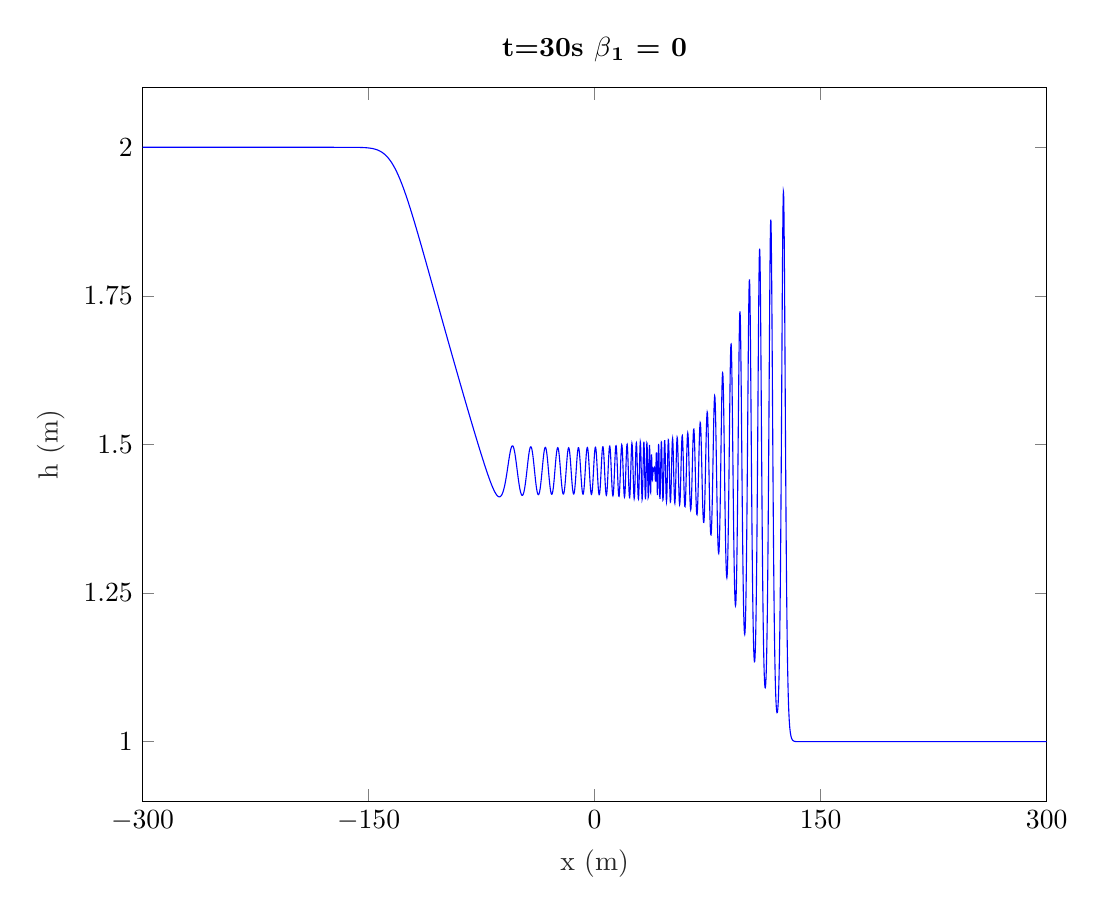
\begin{tikzpicture}

\begin{axis}[%
width=4.521in,
height=3.566in,
at={(0.758in,0.481in)},
scale only axis,
xmin=-300,
xmax=300,
xtick={-300, -150,    0,  150,  300},
xlabel style={font=\color{white!15!black}},
xlabel={x (m)},
ymin=0.9,
ymax=2.1,
ytick={   1, 1.25,  1.5, 1.75,    2},
ylabel style={font=\color{white!15!black}},
ylabel={h (m)},
axis background/.style={fill=white},
title style={font=\bfseries},
title={$\text{t=30s   }\beta{}_\text{1}\text{ = 0}$}
]
\addplot [color=blue, forget plot]
  table[row sep=crcr]{%
-300.18000900045	2\\
-300.030001500075	2\\
-299.8799939997	2\\
-299.729986499325	2\\
-299.57997899895	2\\
-299.429971498575	2\\
-299.2799639982	2\\
-299.129956497825	2\\
-298.97994899745	2\\
-298.829941497075	2\\
-298.6799339967	2\\
-298.529926496325	2\\
-298.37991899595	2\\
-298.229911495575	2\\
-298.0799039952	2\\
-297.929896494825	2\\
-297.77988899445	2\\
-297.629881494075	2\\
-297.4798739937	2\\
-297.329866493325	2\\
-297.17985899295	2\\
-297.029851492575	2\\
-296.8798439922	2\\
-296.729836491825	2\\
-296.57982899145	2\\
-296.429821491075	2\\
-296.2798139907	2\\
-296.129806490325	2\\
-295.979798989949	2\\
-295.829791489574	2\\
-295.679783989199	2\\
-295.529776488824	2\\
-295.379768988449	2\\
-295.229761488074	2\\
-295.079753987699	2\\
-294.929746487324	2\\
-294.779738986949	2\\
-294.629731486574	2\\
-294.479723986199	2\\
-294.329716485824	2\\
-294.179708985449	2\\
-294.029701485074	2\\
-293.879693984699	2\\
-293.729686484324	2\\
-293.579678983949	2\\
-293.429671483574	2\\
-293.279663983199	2\\
-293.129656482824	2\\
-292.979648982449	2\\
-292.829641482074	2\\
-292.679633981699	2\\
-292.529626481324	2\\
-292.379618980949	2\\
-292.229611480574	2\\
-292.079603980199	2\\
-291.929596479824	2\\
-291.779588979449	2\\
-291.629581479074	2\\
-291.479573978699	2\\
-291.329566478324	2\\
-291.179558977949	2\\
-291.029551477574	2\\
-290.879543977199	2\\
-290.729536476824	2\\
-290.579528976449	2\\
-290.429521476074	2\\
-290.279513975699	2\\
-290.129506475324	2\\
-289.979498974949	2\\
-289.829491474574	2\\
-289.679483974199	2\\
-289.529476473824	2\\
-289.379468973449	2\\
-289.229461473074	2\\
-289.079453972699	2\\
-288.929446472324	2\\
-288.779438971949	2\\
-288.629431471574	2\\
-288.479423971199	2\\
-288.329416470824	2\\
-288.179408970449	2\\
-288.029401470073	2\\
-287.879393969698	2\\
-287.729386469323	2\\
-287.579378968948	2\\
-287.429371468573	2\\
-287.279363968198	2\\
-287.129356467823	2\\
-286.979348967448	2\\
-286.829341467073	2\\
-286.679333966698	2\\
-286.529326466323	2\\
-286.379318965948	2\\
-286.229311465573	2\\
-286.079303965198	2\\
-285.929296464823	2\\
-285.779288964448	2\\
-285.629281464073	2\\
-285.479273963698	2\\
-285.329266463323	2\\
-285.179258962948	2\\
-285.029251462573	2\\
-284.879243962198	2\\
-284.729236461823	2\\
-284.579228961448	2\\
-284.429221461073	2\\
-284.279213960698	2\\
-284.129206460323	2\\
-283.979198959948	2\\
-283.829191459573	2\\
-283.679183959198	2\\
-283.529176458823	2\\
-283.379168958448	2\\
-283.229161458073	2\\
-283.079153957698	2\\
-282.929146457323	2\\
-282.779138956948	2\\
-282.629131456573	2\\
-282.479123956198	2\\
-282.329116455823	2\\
-282.179108955448	2\\
-282.029101455073	2\\
-281.879093954698	2\\
-281.729086454323	2\\
-281.579078953948	2\\
-281.429071453573	2\\
-281.279063953198	2\\
-281.129056452823	2\\
-280.979048952448	2\\
-280.829041452073	2\\
-280.679033951698	2\\
-280.529026451323	2\\
-280.379018950948	2\\
-280.229011450573	2\\
-280.079003950197	2\\
-279.928996449822	2\\
-279.778988949447	2\\
-279.628981449072	2\\
-279.478973948697	2\\
-279.328966448322	2\\
-279.178958947947	2\\
-279.028951447572	2\\
-278.878943947197	2\\
-278.728936446822	2\\
-278.578928946447	2\\
-278.428921446072	2\\
-278.278913945697	2\\
-278.128906445322	2\\
-277.978898944947	2\\
-277.828891444572	2\\
-277.678883944197	2\\
-277.528876443822	2\\
-277.378868943447	2\\
-277.228861443072	2\\
-277.078853942697	2\\
-276.928846442322	2\\
-276.778838941947	2\\
-276.628831441572	2\\
-276.478823941197	2\\
-276.328816440822	2\\
-276.178808940447	2\\
-276.028801440072	2\\
-275.878793939697	2\\
-275.728786439322	2\\
-275.578778938947	2\\
-275.428771438572	2\\
-275.278763938197	2\\
-275.128756437822	2\\
-274.978748937447	2\\
-274.828741437072	2\\
-274.678733936697	2\\
-274.528726436322	2\\
-274.378718935947	2\\
-274.228711435572	2\\
-274.078703935197	2\\
-273.928696434822	2\\
-273.778688934447	2\\
-273.628681434072	2\\
-273.478673933697	2\\
-273.328666433322	2\\
-273.178658932947	2\\
-273.028651432572	2\\
-272.878643932197	2\\
-272.728636431822	2\\
-272.578628931447	2\\
-272.428621431072	2\\
-272.278613930697	2\\
-272.128606430321	2\\
-271.978598929946	2\\
-271.828591429571	2\\
-271.678583929196	2\\
-271.528576428821	2\\
-271.378568928446	2\\
-271.228561428071	2\\
-271.078553927696	2\\
-270.928546427321	2\\
-270.778538926946	2\\
-270.628531426571	2\\
-270.478523926196	2\\
-270.328516425821	2\\
-270.178508925446	2\\
-270.028501425071	2\\
-269.878493924696	2\\
-269.728486424321	2\\
-269.578478923946	2\\
-269.428471423571	2\\
-269.278463923196	2\\
-269.128456422821	2\\
-268.978448922446	2\\
-268.828441422071	2\\
-268.678433921696	2\\
-268.528426421321	2\\
-268.378418920946	2\\
-268.228411420571	2\\
-268.078403920196	2\\
-267.928396419821	2\\
-267.778388919446	2\\
-267.628381419071	2\\
-267.478373918696	2\\
-267.328366418321	2\\
-267.178358917946	2\\
-267.028351417571	2\\
-266.878343917196	2\\
-266.728336416821	2\\
-266.578328916446	2\\
-266.428321416071	2\\
-266.278313915696	2\\
-266.128306415321	2\\
-265.978298914946	2\\
-265.828291414571	2\\
-265.678283914196	2\\
-265.528276413821	2\\
-265.378268913446	2\\
-265.228261413071	2\\
-265.078253912696	2\\
-264.928246412321	2\\
-264.778238911946	2\\
-264.628231411571	2\\
-264.478223911196	2\\
-264.328216410821	2\\
-264.178208910446	2\\
-264.02820141007	2\\
-263.878193909695	2\\
-263.72818640932	2\\
-263.578178908945	2\\
-263.42817140857	2\\
-263.278163908195	2\\
-263.12815640782	2\\
-262.978148907445	2\\
-262.82814140707	2\\
-262.678133906695	2\\
-262.52812640632	2\\
-262.378118905945	2\\
-262.22811140557	2\\
-262.078103905195	2\\
-261.92809640482	2\\
-261.778088904445	2\\
-261.62808140407	2\\
-261.478073903695	2\\
-261.32806640332	2\\
-261.178058902945	2\\
-261.02805140257	2\\
-260.878043902195	2\\
-260.72803640182	2\\
-260.578028901445	2\\
-260.42802140107	2\\
-260.278013900695	2\\
-260.12800640032	2\\
-259.977998899945	2\\
-259.82799139957	2\\
-259.677983899195	2\\
-259.52797639882	2\\
-259.377968898445	2\\
-259.22796139807	2\\
-259.077953897695	2\\
-258.92794639732	2\\
-258.777938896945	2\\
-258.62793139657	2\\
-258.477923896195	2\\
-258.32791639582	2\\
-258.177908895445	2\\
-258.02790139507	2\\
-257.877893894695	2\\
-257.72788639432	2\\
-257.577878893945	2\\
-257.42787139357	2\\
-257.277863893195	2\\
-257.12785639282	2\\
-256.977848892445	2\\
-256.82784139207	2\\
-256.677833891695	2\\
-256.52782639132	2\\
-256.377818890945	2\\
-256.22781139057	2\\
-256.077803890195	2\\
-255.927796389819	2\\
-255.777788889444	2\\
-255.627781389069	2\\
-255.477773888694	2\\
-255.327766388319	2\\
-255.177758887944	2\\
-255.027751387569	2\\
-254.877743887194	2\\
-254.727736386819	2\\
-254.577728886444	2\\
-254.427721386069	2\\
-254.277713885694	2\\
-254.127706385319	2\\
-253.977698884944	2\\
-253.827691384569	2\\
-253.677683884194	2\\
-253.527676383819	2\\
-253.377668883444	2\\
-253.227661383069	2\\
-253.077653882694	2\\
-252.927646382319	2\\
-252.777638881944	2\\
-252.627631381569	2\\
-252.477623881194	2\\
-252.327616380819	2\\
-252.177608880444	2\\
-252.027601380069	2\\
-251.877593879694	2\\
-251.727586379319	2\\
-251.577578878944	2\\
-251.427571378569	2\\
-251.277563878194	2\\
-251.127556377819	2\\
-250.977548877444	2\\
-250.827541377069	2\\
-250.677533876694	2\\
-250.527526376319	2\\
-250.377518875944	2\\
-250.227511375569	2\\
-250.077503875194	2\\
-249.927496374819	2\\
-249.777488874444	2\\
-249.627481374069	2\\
-249.477473873694	2\\
-249.327466373319	2\\
-249.177458872944	2\\
-249.027451372569	2\\
-248.877443872194	2\\
-248.727436371819	2\\
-248.577428871444	2\\
-248.427421371069	2\\
-248.277413870694	2\\
-248.127406370319	2\\
-247.977398869943	2\\
-247.827391369568	2\\
-247.677383869193	2\\
-247.527376368818	2\\
-247.377368868443	2\\
-247.227361368068	2\\
-247.077353867693	2\\
-246.927346367318	2\\
-246.777338866943	2\\
-246.627331366568	2\\
-246.477323866193	2\\
-246.327316365818	2\\
-246.177308865443	2\\
-246.027301365068	2\\
-245.877293864693	2\\
-245.727286364318	2\\
-245.577278863943	2\\
-245.427271363568	2\\
-245.277263863193	2\\
-245.127256362818	2\\
-244.977248862443	2\\
-244.827241362068	2\\
-244.677233861693	2\\
-244.527226361318	2\\
-244.377218860943	2\\
-244.227211360568	2\\
-244.077203860193	2\\
-243.927196359818	2\\
-243.777188859443	2\\
-243.627181359068	2\\
-243.477173858693	2\\
-243.327166358318	2\\
-243.177158857943	2\\
-243.027151357568	2\\
-242.877143857193	2\\
-242.727136356818	2\\
-242.577128856443	2\\
-242.427121356068	2\\
-242.277113855693	2\\
-242.127106355318	2\\
-241.977098854943	2\\
-241.827091354568	2\\
-241.677083854193	2\\
-241.527076353818	2\\
-241.377068853443	2\\
-241.227061353068	2\\
-241.077053852693	2\\
-240.927046352318	2\\
-240.777038851943	2\\
-240.627031351568	2\\
-240.477023851193	2\\
-240.327016350818	2\\
-240.177008850443	2\\
-240.027001350068	2\\
-239.876993849692	2\\
-239.726986349317	2\\
-239.576978848942	2\\
-239.426971348567	2\\
-239.276963848192	2\\
-239.126956347817	2\\
-238.976948847442	2\\
-238.826941347067	2\\
-238.676933846692	2\\
-238.526926346317	2\\
-238.376918845942	2\\
-238.226911345567	2\\
-238.076903845192	2\\
-237.926896344817	2\\
-237.776888844442	2\\
-237.626881344067	2\\
-237.476873843692	2\\
-237.326866343317	2\\
-237.176858842942	2\\
-237.026851342567	2\\
-236.876843842192	2\\
-236.726836341817	2\\
-236.576828841442	2\\
-236.426821341067	2\\
-236.276813840692	2\\
-236.126806340317	2\\
-235.976798839942	2\\
-235.826791339567	2\\
-235.676783839192	2\\
-235.526776338817	2\\
-235.376768838442	2\\
-235.226761338067	2\\
-235.076753837692	2\\
-234.926746337317	2\\
-234.776738836942	2\\
-234.626731336567	2\\
-234.476723836192	2\\
-234.326716335817	2\\
-234.176708835442	2\\
-234.026701335067	2\\
-233.876693834692	2\\
-233.726686334317	2\\
-233.576678833942	2\\
-233.426671333567	2\\
-233.276663833192	2\\
-233.126656332817	2\\
-232.976648832442	2\\
-232.826641332067	2\\
-232.676633831692	2\\
-232.526626331317	2\\
-232.376618830942	2\\
-232.226611330567	2\\
-232.076603830192	2\\
-231.926596329817	2\\
-231.776588829441	2\\
-231.626581329066	2\\
-231.476573828691	2\\
-231.326566328316	2\\
-231.176558827941	2\\
-231.026551327566	2\\
-230.876543827191	2\\
-230.726536326816	2\\
-230.576528826441	2\\
-230.426521326066	2\\
-230.276513825691	2\\
-230.126506325316	2\\
-229.976498824941	2\\
-229.826491324566	2\\
-229.676483824191	2\\
-229.526476323816	2\\
-229.376468823441	2\\
-229.226461323066	2\\
-229.076453822691	2\\
-228.926446322316	2\\
-228.776438821941	2\\
-228.626431321566	2\\
-228.476423821191	2\\
-228.326416320816	2\\
-228.176408820441	2\\
-228.026401320066	2\\
-227.876393819691	2\\
-227.726386319316	2\\
-227.576378818941	2\\
-227.426371318566	2\\
-227.276363818191	2\\
-227.126356317816	2\\
-226.976348817441	2\\
-226.826341317066	2\\
-226.676333816691	2\\
-226.526326316316	2\\
-226.376318815941	2\\
-226.226311315566	2\\
-226.076303815191	2\\
-225.926296314816	2\\
-225.776288814441	2\\
-225.626281314066	2\\
-225.476273813691	2\\
-225.326266313316	2\\
-225.176258812941	2\\
-225.026251312566	2\\
-224.876243812191	2\\
-224.726236311816	2\\
-224.576228811441	2\\
-224.426221311066	2\\
-224.276213810691	2\\
-224.126206310316	2\\
-223.976198809941	2\\
-223.826191309565	2\\
-223.67618380919	2\\
-223.526176308815	2\\
-223.37616880844	2\\
-223.226161308065	2\\
-223.07615380769	2\\
-222.926146307315	2\\
-222.77613880694	2\\
-222.626131306565	2\\
-222.47612380619	2\\
-222.326116305815	2\\
-222.17610880544	2\\
-222.026101305065	2\\
-221.87609380469	2\\
-221.726086304315	2\\
-221.57607880394	2\\
-221.426071303565	2\\
-221.27606380319	2\\
-221.126056302815	2\\
-220.97604880244	2\\
-220.826041302065	2\\
-220.67603380169	2\\
-220.526026301315	2\\
-220.37601880094	2\\
-220.226011300565	2\\
-220.07600380019	2\\
-219.925996299815	2\\
-219.77598879944	2\\
-219.625981299065	2\\
-219.47597379869	2\\
-219.325966298315	2\\
-219.17595879794	2\\
-219.025951297565	2\\
-218.87594379719	2\\
-218.725936296815	2\\
-218.57592879644	2\\
-218.425921296065	2\\
-218.27591379569	2\\
-218.125906295315	2\\
-217.97589879494	2\\
-217.825891294565	2\\
-217.67588379419	2\\
-217.525876293815	2\\
-217.37586879344	2\\
-217.225861293065	2\\
-217.07585379269	2\\
-216.925846292315	2\\
-216.77583879194	2\\
-216.625831291565	2\\
-216.47582379119	2\\
-216.325816290815	2\\
-216.17580879044	2\\
-216.025801290065	2\\
-215.875793789689	2\\
-215.725786289314	2\\
-215.575778788939	2\\
-215.425771288564	2\\
-215.275763788189	2\\
-215.125756287814	2\\
-214.975748787439	2\\
-214.825741287064	1.99999999999999\\
-214.675733786689	1.99999999999999\\
-214.525726286314	1.99999999999999\\
-214.375718785939	1.99999999999999\\
-214.225711285564	1.99999999999999\\
-214.075703785189	1.99999999999998\\
-213.925696284814	1.99999999999998\\
-213.775688784439	1.99999999999998\\
-213.625681284064	1.99999999999998\\
-213.475673783689	1.99999999999997\\
-213.325666283314	1.99999999999997\\
-213.175658782939	1.99999999999996\\
-213.025651282564	1.99999999999996\\
-212.875643782189	1.99999999999996\\
-212.725636281814	1.99999999999995\\
-212.575628781439	1.99999999999995\\
-212.425621281064	1.99999999999994\\
-212.275613780689	1.99999999999994\\
-212.125606280314	1.99999999999993\\
-211.975598779939	1.99999999999992\\
-211.825591279564	1.99999999999992\\
-211.675583779189	1.99999999999991\\
-211.525576278814	1.9999999999999\\
-211.375568778439	1.99999999999989\\
-211.225561278064	1.99999999999989\\
-211.075553777689	1.99999999999988\\
-210.925546277314	1.99999999999987\\
-210.775538776939	1.99999999999985\\
-210.625531276564	1.99999999999984\\
-210.475523776189	1.99999999999983\\
-210.325516275814	1.99999999999982\\
-210.175508775439	1.9999999999998\\
-210.025501275064	1.99999999999979\\
-209.875493774689	1.99999999999977\\
-209.725486274314	1.99999999999975\\
-209.575478773939	1.99999999999973\\
-209.425471273564	1.99999999999971\\
-209.275463773189	1.99999999999969\\
-209.125456272814	1.99999999999967\\
-208.975448772439	1.99999999999965\\
-208.825441272064	1.99999999999962\\
-208.675433771689	1.99999999999959\\
-208.525426271314	1.99999999999956\\
-208.375418770939	1.99999999999953\\
-208.225411270564	1.9999999999995\\
-208.075403770189	1.99999999999946\\
-207.925396269813	1.99999999999942\\
-207.775388769438	1.99999999999938\\
-207.625381269063	1.99999999999933\\
-207.475373768688	1.99999999999929\\
-207.325366268313	1.99999999999924\\
-207.175358767938	1.99999999999918\\
-207.025351267563	1.99999999999912\\
-206.875343767188	1.99999999999906\\
-206.725336266813	1.999999999999\\
-206.575328766438	1.99999999999892\\
-206.425321266063	1.99999999999885\\
-206.275313765688	1.99999999999877\\
-206.125306265313	1.99999999999868\\
-205.975298764938	1.99999999999859\\
-205.825291264563	1.99999999999849\\
-205.675283764188	1.99999999999839\\
-205.525276263813	1.99999999999827\\
-205.375268763438	1.99999999999816\\
-205.225261263063	1.99999999999803\\
-205.075253762688	1.99999999999789\\
-204.925246262313	1.99999999999775\\
-204.775238761938	1.99999999999759\\
-204.625231261563	1.99999999999742\\
-204.475223761188	1.99999999999725\\
-204.325216260813	1.99999999999706\\
-204.175208760438	1.99999999999686\\
-204.025201260063	1.99999999999664\\
-203.875193759688	1.99999999999641\\
-203.725186259313	1.99999999999617\\
-203.575178758938	1.9999999999959\\
-203.425171258563	1.99999999999562\\
-203.275163758188	1.99999999999532\\
-203.125156257813	1.99999999999501\\
-202.975148757438	1.99999999999467\\
-202.825141257063	1.9999999999943\\
-202.675133756688	1.99999999999392\\
-202.525126256313	1.9999999999935\\
-202.375118755938	1.99999999999306\\
-202.225111255563	1.99999999999259\\
-202.075103755188	1.99999999999209\\
-201.925096254813	1.99999999999156\\
-201.775088754438	1.99999999999099\\
-201.625081254063	1.99999999999038\\
-201.475073753688	1.99999999998973\\
-201.325066253313	1.99999999998904\\
-201.175058752938	1.9999999999883\\
-201.025051252563	1.99999999998752\\
-200.875043752188	1.99999999998668\\
-200.725036251813	1.99999999998579\\
-200.575028751438	1.99999999998483\\
-200.425021251063	1.99999999998382\\
-200.275013750688	1.99999999998274\\
-200.125006250313	1.99999999998158\\
-199.974998749937	1.99999999998035\\
-199.824991249562	1.99999999997904\\
-199.674983749187	1.99999999997764\\
-199.524976248812	1.99999999997616\\
-199.374968748437	1.99999999997457\\
-199.224961248062	1.99999999997288\\
-199.074953747687	1.99999999997108\\
-198.924946247312	1.99999999996916\\
-198.774938746937	1.99999999996711\\
-198.624931246562	1.99999999996493\\
-198.474923746187	1.99999999996261\\
-198.324916245812	1.99999999996014\\
-198.174908745437	1.99999999995751\\
-198.024901245062	1.9999999999547\\
-197.874893744687	1.99999999995171\\
-197.724886244312	1.99999999994853\\
-197.574878743937	1.99999999994514\\
-197.424871243562	1.99999999994153\\
-197.274863743187	1.99999999993768\\
-197.124856242812	1.99999999993359\\
-196.974848742437	1.99999999992923\\
-196.824841242062	1.99999999992459\\
-196.674833741687	1.99999999991965\\
-196.524826241312	1.99999999991439\\
-196.374818740937	1.99999999990879\\
-196.224811240562	1.99999999990283\\
-196.074803740187	1.99999999989648\\
-195.924796239812	1.99999999988973\\
-195.774788739437	1.99999999988254\\
-195.624781239062	1.99999999987489\\
-195.474773738687	1.99999999986675\\
-195.324766238312	1.99999999985808\\
-195.174758737937	1.99999999984886\\
-195.024751237562	1.99999999983906\\
-194.874743737187	1.99999999982862\\
-194.724736236812	1.99999999981752\\
-194.574728736437	1.9999999998057\\
-194.424721236062	1.99999999979314\\
-194.274713735687	1.99999999977977\\
-194.124706235312	1.99999999976555\\
-193.974698734937	1.99999999975043\\
-193.824691234562	1.99999999973435\\
-193.674683734187	1.99999999971724\\
-193.524676233812	1.99999999969905\\
-193.374668733437	1.99999999967971\\
-193.224661233062	1.99999999965914\\
-193.074653732687	1.99999999963727\\
-192.924646232312	1.99999999961402\\
-192.774638731937	1.9999999995893\\
-192.624631231562	1.99999999956302\\
-192.474623731187	1.99999999953509\\
-192.324616230812	1.9999999995054\\
-192.174608730437	1.99999999947384\\
-192.024601230062	1.9999999994403\\
-191.874593729686	1.99999999940465\\
-191.724586229311	1.99999999936677\\
-191.574578728936	1.99999999932651\\
-191.424571228561	1.99999999928373\\
-191.274563728186	1.99999999923828\\
-191.124556227811	1.99999999919\\
-190.974548727436	1.99999999913869\\
-190.824541227061	1.99999999908419\\
-190.674533726686	1.9999999990263\\
-190.524526226311	1.9999999989648\\
-190.374518725936	1.99999999889949\\
-190.224511225561	1.99999999883011\\
-190.074503725186	1.99999999875644\\
-189.924496224811	1.9999999986782\\
-189.774488724436	1.99999999859512\\
-189.624481224061	1.9999999985069\\
-189.474473723686	1.99999999841323\\
-189.324466223311	1.99999999831379\\
-189.174458722936	1.99999999820821\\
-189.024451222561	1.99999999809613\\
-188.874443722186	1.99999999797716\\
-188.724436221811	1.99999999785087\\
-188.574428721436	1.99999999771684\\
-188.424421221061	1.99999999757459\\
-188.274413720686	1.99999999742362\\
-188.124406220311	1.99999999726342\\
-187.974398719936	1.99999999709343\\
-187.824391219561	1.99999999691305\\
-187.674383719186	1.99999999672168\\
-187.524376218811	1.99999999651865\\
-187.374368718436	1.99999999630326\\
-187.224361218061	1.99999999607477\\
-187.074353717686	1.99999999583242\\
-186.924346217311	1.99999999557536\\
-186.774338716936	1.99999999530272\\
-186.624331216561	1.99999999501358\\
-186.474323716186	1.99999999470697\\
-186.324316215811	1.99999999438183\\
-186.174308715436	1.99999999403708\\
-186.024301215061	1.99999999367156\\
-185.874293714686	1.99999999328404\\
-185.724286214311	1.99999999287322\\
-185.574278713936	1.99999999243772\\
-185.424271213561	1.9999999919761\\
-185.274263713186	1.99999999148683\\
-185.124256212811	1.99999999096827\\
-184.974248712436	1.99999999041871\\
-184.824241212061	1.99999998983634\\
-184.674233711686	1.99999998921923\\
-184.524226211311	1.99999998856536\\
-184.374218710936	1.99999998787258\\
-184.224211210561	1.99999998713863\\
-184.074203710186	1.9999999863611\\
-183.92419620981	1.99999998553747\\
-183.774188709435	1.99999998466506\\
-183.62418120906	1.99999998374105\\
-183.474173708685	1.99999998276244\\
-183.32416620831	1.99999998172607\\
-183.174158707935	1.99999998062862\\
-183.02415120756	1.99999997946656\\
-182.874143707185	1.99999997823617\\
-182.72413620681	1.99999997693352\\
-182.574128706435	1.99999997555445\\
-182.42412120606	1.99999997409459\\
-182.274113705685	1.99999997254931\\
-182.12410620531	1.99999997091372\\
-181.974098704935	1.99999996918266\\
-181.82409120456	1.99999996735067\\
-181.674083704185	1.99999996541203\\
-181.52407620381	1.99999996336064\\
-181.374068703435	1.99999996119011\\
-181.22406120306	1.99999995889367\\
-181.074053702685	1.9999999564642\\
-180.92404620231	1.99999995389415\\
-180.774038701935	1.9999999511756\\
-180.62403120156	1.99999994830016\\
-180.474023701185	1.99999994525898\\
-180.32401620081	1.99999994204274\\
-180.174008700435	1.99999993864161\\
-180.02400120006	1.99999993504521\\
-179.873993699685	1.9999999312426\\
-179.72398619931	1.99999992722223\\
-179.573978698935	1.99999992297196\\
-179.42397119856	1.99999991847894\\
-179.273963698185	1.99999991372966\\
-179.12395619781	1.99999990870986\\
-178.973948697435	1.99999990340452\\
-178.82394119706	1.9999998977978\\
-178.673933696685	1.999999891873\\
-178.52392619631	1.99999988561255\\
-178.373918695935	1.99999987899791\\
-178.22391119556	1.99999987200955\\
-178.073903695185	1.9999998646269\\
-177.92389619481	1.99999985682828\\
-177.773888694435	1.99999984859088\\
-177.62388119406	1.99999983989064\\
-177.473873693685	1.99999983070225\\
-177.32386619331	1.99999982099903\\
-177.173858692935	1.99999981075292\\
-177.02385119256	1.99999979993433\\
-176.873843692185	1.99999978851216\\
-176.72383619181	1.99999977645363\\
-176.573828691435	1.99999976372426\\
-176.42382119106	1.99999975028774\\
-176.273813690685	1.99999973610587\\
-176.123806190309	1.99999972113845\\
-175.973798689934	1.99999970534316\\
-175.823791189559	1.99999968867552\\
-175.673783689184	1.99999967108868\\
-175.523776188809	1.9999996525334\\
-175.373768688434	1.99999963295786\\
-175.223761188059	1.99999961230757\\
-175.073753687684	1.99999959052522\\
-174.923746187309	1.99999956755055\\
-174.773738686934	1.9999995433202\\
-174.623731186559	1.99999951776755\\
-174.473723686184	1.99999949082256\\
-174.323716185809	1.99999946241163\\
-174.173708685434	1.99999943245738\\
-174.023701185059	1.99999940087849\\
-173.873693684684	1.99999936758951\\
-173.723686184309	1.99999933250064\\
-173.573678683934	1.99999929551756\\
-173.423671183559	1.99999925654114\\
-173.273663683184	1.99999921546728\\
-173.123656182809	1.99999917218663\\
-172.973648682434	1.99999912658434\\
-172.823641182059	1.99999907853981\\
-172.673633681684	1.99999902792639\\
-172.523626181309	1.99999897461111\\
-172.373618680934	1.9999989184544\\
-172.223611180559	1.99999885930971\\
-172.073603680184	1.99999879702323\\
-171.923596179809	1.99999873143356\\
-171.773588679434	1.99999866237129\\
-171.623581179059	1.99999858965867\\
-171.473573678684	1.99999851310921\\
-171.323566178309	1.99999843252728\\
-171.173558677934	1.99999834770762\\
-171.023551177559	1.999998258435\\
-170.873543677184	1.99999816448364\\
-170.723536176809	1.99999806561682\\
-170.573528676434	1.99999796158631\\
-170.423521176059	1.99999785213185\\
-170.273513675684	1.99999773698061\\
-170.123506175309	1.99999761584663\\
-169.973498674934	1.99999748843016\\
-169.823491174559	1.99999735441709\\
-169.673483674184	1.99999721347828\\
-169.523476173809	1.99999706526885\\
-169.373468673434	1.99999690942751\\
-169.223461173059	1.99999674557579\\
-169.073453672684	1.99999657331728\\
-168.923446172309	1.99999639223683\\
-168.773438671934	1.99999620189968\\
-168.623431171559	1.99999600185064\\
-168.473423671184	1.99999579161314\\
-168.323416170809	1.9999955706883\\
-168.173408670434	1.99999533855392\\
-168.023401170058	1.9999950946635\\
-167.873393669683	1.99999483844515\\
-167.723386169308	1.99999456930044\\
-167.573378668933	1.99999428660331\\
-167.423371168558	1.99999398969884\\
-167.273363668183	1.99999367790199\\
-167.123356167808	1.99999335049628\\
-166.973348667433	1.99999300673252\\
-166.823341167058	1.99999264582731\\
-166.673333666683	1.99999226696164\\
-166.523326166308	1.99999186927933\\
-166.373318665933	1.9999914518855\\
-166.223311165558	1.99999101384489\\
-166.073303665183	1.9999905541802\\
-165.923296164808	1.99999007187027\\
-165.773288664433	1.99998956584829\\
-165.623281164058	1.9999890349999\\
-165.473273663683	1.99998847816117\\
-165.323266163308	1.99998789411658\\
-165.173258662933	1.99998728159692\\
-165.023251162558	1.99998663927702\\
-164.873243662183	1.99998596577352\\
-164.723236161808	1.99998525964245\\
-164.573228661433	1.99998451937684\\
-164.423221161058	1.99998374340408\\
-164.273213660683	1.99998293008335\\
-164.123206160308	1.99998207770287\\
-163.973198659933	1.99998118447706\\
-163.823191159558	1.99998024854358\\
-163.673183659183	1.99997926796034\\
-163.523176158808	1.99997824070232\\
-163.373168658433	1.99997716465833\\
-163.223161158058	1.99997603762766\\
-163.073153657683	1.99997485731656\\
-162.923146157308	1.99997362133464\\
-162.773138656933	1.99997232719118\\
-162.623131156558	1.99997097229126\\
-162.473123656183	1.99996955393179\\
-162.323116155808	1.99996806929734\\
-162.173108655433	1.99996651545601\\
-162.023101155058	1.99996488935491\\
-161.873093654683	1.99996318781572\\
-161.723086154308	1.99996140753\\
-161.573078653933	1.99995954505432\\
-161.423071153558	1.99995759680535\\
-161.273063653183	1.99995555905464\\
-161.123056152808	1.99995342792341\\
-160.973048652433	1.99995119937704\\
-160.823041152058	1.99994886921943\\
-160.673033651683	1.99994643308726\\
-160.523026151308	1.99994388644395\\
-160.373018650933	1.99994122457356\\
-160.223011150558	1.99993844257441\\
-160.073003650182	1.99993553535261\\
-159.922996149807	1.99993249761533\\
-159.772988649432	1.99992932386387\\
-159.622981149057	1.99992600838663\\
-159.472973648682	1.99992254525175\\
-159.322966148307	1.99991892829968\\
-159.172958647932	1.99991515113539\\
-159.022951147557	1.99991120712057\\
-158.872943647182	1.99990708936541\\
-158.722936146807	1.99990279072031\\
-158.572928646432	1.99989830376734\\
-158.422921146057	1.99989362081145\\
-158.272913645682	1.99988873387144\\
-158.122906145307	1.99988363467081\\
-157.972898644932	1.99987831462826\\
-157.822891144557	1.99987276484803\\
-157.672883644182	1.99986697611002\\
-157.522876143807	1.99986093885958\\
-157.372868643432	1.99985464319721\\
-157.222861143057	1.99984807886794\\
-157.072853642682	1.99984123525043\\
-156.922846142307	1.99983410134594\\
-156.772838641932	1.99982666576703\\
-156.622831141557	1.99981891672593\\
-156.472823641182	1.99981084202282\\
-156.322816140807	1.99980242903375\\
-156.172808640432	1.99979366469842\\
-156.022801140057	1.99978453550764\\
-155.872793639682	1.9997750274906\\
-155.722786139307	1.99976512620196\\
-155.572778638932	1.99975481670859\\
-155.422771138557	1.99974408357617\\
-155.272763638182	1.9997329108556\\
-155.122756137807	1.99972128206908\\
-154.972748637432	1.99970918019608\\
-154.822741137057	1.99969658765902\\
-154.672733636682	1.99968348630884\\
-154.522726136307	1.99966985741028\\
-154.372718635932	1.99965568162702\\
-154.222711135557	1.99964093900664\\
-154.072703635182	1.99962560896537\\
-153.922696134807	1.99960967027269\\
-153.772688634432	1.9995931010358\\
-153.622681134057	1.9995758786839\\
-153.472673633682	1.99955797995235\\
-153.322666133307	1.99953938086672\\
-153.172658632932	1.99952005672668\\
-153.022651132557	1.99949998208986\\
-152.872643632182	1.99947913075555\\
-152.722636131807	1.99945747574838\\
-152.572628631432	1.99943498930191\\
-152.422621131057	1.99941164284221\\
-152.272613630682	1.9993874069714\\
-152.122606130307	1.99936225145114\\
-151.972598629931	1.99933614518623\\
-151.822591129556	1.99930905620817\\
-151.672583629181	1.9992809516588\\
-151.522576128806	1.99925179777398\\
-151.372568628431	1.99922155986744\\
-151.222561128056	1.99919020231467\\
-151.072553627681	1.99915768853702\\
-150.922546127306	1.99912398098592\\
-150.772538626931	1.99908904112736\\
-150.622531126556	1.99905282942651\\
-150.472523626181	1.9990153053327\\
-150.322516125806	1.99897642726456\\
-150.172508625431	1.99893615259558\\
-150.022501125056	1.99889443763997\\
-149.872493624681	1.99885123763886\\
-149.722486124306	1.99880650674698\\
-149.572478623931	1.99876019801974\\
-149.422471123556	1.99871226340078\\
-149.272463623181	1.99866265371006\\
-149.122456122806	1.99861131863247\\
-148.972448622431	1.99855820670705\\
-148.822441122056	1.99850326531681\\
-148.672433621681	1.99844644067925\\
-148.522426121306	1.99838767783752\\
-148.372418620931	1.99832692065235\\
-148.222411120556	1.99826411179481\\
-148.072403620181	1.99819919273978\\
-147.922396119806	1.99813210376038\\
-147.772388619431	1.99806278392324\\
-147.622381119056	1.99799117108476\\
-147.472373618681	1.99791720188831\\
-147.322366118306	1.99784081176249\\
-147.172358617931	1.99776193492044\\
-147.022351117556	1.99768050436027\\
-146.872343617181	1.99759645186663\\
-146.722336116806	1.9975097080135\\
-146.572328616431	1.99742020216814\\
-146.422321116056	1.99732786249644\\
-146.272313615681	1.99723261596947\\
-146.122306115306	1.99713438837143\\
-145.972298614931	1.99703310430898\\
-145.822291114556	1.99692868722203\\
-145.672283614181	1.99682105939594\\
-145.522276113806	1.9967101419753\\
-145.372268613431	1.99659585497915\\
-145.222261113056	1.99647811731784\\
-145.072253612681	1.99635684681147\\
-144.922246112306	1.99623196020997\\
-144.772238611931	1.99610337321479\\
-144.622231111556	1.99597100050232\\
-144.472223611181	1.99583475574903\\
-144.322216110806	1.99569455165826\\
-144.172208610431	1.99555029998886\\
-144.022201110056	1.99540191158552\\
-143.87219360968	1.9952492964109\\
-143.722186109305	1.99509236357955\\
-143.57217860893	1.99493102139364\\
-143.422171108555	1.99476517738048\\
-143.27216360818	1.99459473833186\\
-143.122156107805	1.99441961034515\\
-142.97214860743	1.9942396988663\\
-142.822141107055	1.99405490873453\\
-142.67213360668	1.99386514422886\\
-142.522126106305	1.99367030911639\\
-142.37211860593	1.99347030670234\\
-142.222111105555	1.99326503988182\\
-142.07210360518	1.99305441119328\\
-141.922096104805	1.99283832287367\\
-141.77208860443	1.99261667691518\\
-141.622081104055	1.99238937512366\\
-141.47207360368	1.99215631917848\\
-141.322066103305	1.99191741069404\\
-141.17205860293	1.99167255128264\\
-141.022051102555	1.99142164261874\\
-140.87204360218	1.99116458650469\\
-140.722036101805	1.99090128493759\\
-140.57202860143	1.99063164017745\\
-140.422021101055	1.99035555481651\\
-140.27201360068	1.99007293184951\\
-140.122006100305	1.98978367474515\\
-139.97199859993	1.9894876875182\\
-139.821991099555	1.9891848748027\\
-139.67198359918	1.98887514192562\\
-139.521976098805	1.98855839498139\\
-139.37196859843	1.9882345409068\\
-139.221961098055	1.98790348755639\\
-139.07195359768	1.98756514377822\\
-138.921946097305	1.98721941948976\\
-138.77193859693	1.98686622575401\\
-138.621931096555	1.98650547485554\\
-138.47192359618	1.98613708037642\\
-138.321916095805	1.985760957272\\
-138.17190859543	1.9853770219463\\
-138.021901095055	1.98498519232687\\
-137.87189359468	1.98458538793919\\
-137.721886094305	1.98417752998029\\
-137.57187859393	1.98376154139158\\
-137.421871093555	1.98333734693066\\
-137.27186359318	1.98290487324219\\
-137.121856092805	1.98246404892741\\
-136.97184859243	1.9820148046125\\
-136.821841092055	1.98155707301538\\
-136.67183359168	1.98109078901106\\
-136.521826091305	1.98061588969522\\
-136.37181859093	1.98013231444609\\
-136.221811090555	1.97964000498438\\
-136.07180359018	1.97913890543125\\
-135.921796089805	1.97862896236407\\
-135.771788589429	1.97811012487003\\
-135.621781089054	1.97758234459746\\
-135.471773588679	1.97704557580458\\
-135.321766088304	1.97649977540592\\
-135.171758587929	1.97594490301598\\
-135.021751087554	1.97538092099028\\
-134.871743587179	1.97480779446362\\
-134.721736086804	1.97422549138549\\
-134.571728586429	1.97363398255256\\
-134.421721086054	1.9730332416382\\
-134.271713585679	1.97242324521897\\
-134.121706085304	1.97180397279796\\
-133.971698584929	1.97117540682512\\
-133.821691084554	1.97053753271425\\
-133.671683584179	1.96989033885691\\
-133.521676083804	1.96923381663305\\
-133.371668583429	1.96856796041831\\
-133.221661083054	1.96789276758821\\
-133.071653582679	1.96720823851886\\
-132.921646082304	1.96651437658459\\
-132.771638581929	1.96581118815212\\
-132.621631081554	1.96509868257159\\
-132.471623581179	1.96437687216435\\
-132.321616080804	1.96364577220741\\
-132.171608580429	1.96290540091486\\
-132.021601080054	1.96215577941607\\
-131.871593579679	1.96139693173077\\
-131.721586079304	1.96062888474112\\
-131.571578578929	1.95985166816077\\
-131.421571078554	1.95906531450104\\
-131.271563578179	1.95826985903414\\
-131.121556077804	1.95746533975373\\
-130.971548577429	1.95665179733268\\
-130.821541077054	1.95582927507823\\
-130.671533576679	1.95499781888466\\
-130.521526076304	1.95415747718352\\
-130.371518575929	1.95330830089143\\
-130.221511075554	1.95245034335575\\
-130.071503575179	1.95158366029806\\
-129.921496074804	1.95070830975568\\
-129.771488574429	1.94982435202114\\
-129.621481074054	1.94893184958002\\
-129.471473573679	1.94803086704697\\
-129.321466073304	1.94712147110028\\
-129.171458572929	1.94620373041488\\
-129.021451072554	1.94527771559415\\
-128.871443572179	1.9443434991004\\
-128.721436071804	1.9434011551844\\
-128.571428571429	1.94245075981383\\
-128.421421071054	1.94149239060099\\
-128.271413570679	1.94052612672975\\
-128.121406070304	1.93955204888194\\
-127.971398569929	1.93857023916327\\
-127.821391069553	1.93758078102888\\
-127.671383569178	1.93658375920866\\
-127.521376068803	1.93557925963256\\
-127.371368568428	1.93456736935571\\
-127.221361068053	1.93354817648386\\
-127.071353567678	1.93252177009893\\
-126.921346067303	1.93148824018488\\
-126.771338566928	1.93044767755414\\
-126.621331066553	1.92940017377442\\
-126.471323566178	1.92834582109629\\
-126.321316065803	1.92728471238143\\
-126.171308565428	1.92621694103169\\
-126.021301065053	1.92514260091912\\
-125.871293564678	1.92406178631693\\
-125.721286064303	1.92297459183157\\
-125.571278563928	1.92188111233595\\
-125.421271063553	1.92078144290385\\
-125.271263563178	1.91967567874564\\
-125.121256062803	1.91856391514538\\
-124.971248562428	1.91744624739924\\
-124.821241062053	1.91632277075551\\
-124.671233561678	1.91519358035599\\
-124.521226061303	1.91405877117903\\
-124.371218560928	1.91291843798411\\
-124.221211060553	1.91177267525813\\
-124.071203560178	1.91062157716326\\
-123.921196059803	1.90946523748659\\
-123.771188559428	1.90830374959146\\
-123.621181059053	1.90713720637049\\
-123.471173558678	1.90596570020044\\
-123.321166058303	1.90478932289882\\
-123.171158557928	1.90360816568223\\
-123.021151057553	1.90242231912656\\
-122.871143557178	1.90123187312892\\
-122.721136056803	1.90003691687139\\
-122.571128556428	1.89883753878653\\
-122.421121056053	1.89763382652465\\
-122.271113555678	1.89642586692291\\
-122.121106055303	1.89521374597606\\
-121.971098554928	1.893997548809\\
-121.821091054553	1.89277735965102\\
-121.671083554178	1.89155326181171\\
-121.521076053803	1.89032533765856\\
-121.371068553428	1.8890936685962\\
-121.221061053053	1.88785833504723\\
-121.071053552678	1.88661941643467\\
-120.921046052303	1.88537699116589\\
-120.771038551928	1.88413113661812\\
-120.621031051553	1.88288192912544\\
-120.471023551178	1.88162944396714\\
-120.321016050803	1.88037375535758\\
-120.171008550428	1.87911493643736\\
-120.021001050052	1.87785305926585\\
-119.870993549677	1.87658819481496\\
-119.720986049302	1.87532041296423\\
-119.570978548927	1.87404978249706\\
-119.420971048552	1.87277637109815\\
-119.270963548177	1.87150024535204\\
-119.120956047802	1.87022147074272\\
-118.970948547427	1.86894011165435\\
-118.820941047052	1.86765623137282\\
-118.670933546677	1.86636989208846\\
-118.520926046302	1.86508115489952\\
-118.370918545927	1.86379007981655\\
-118.220911045552	1.86249672576765\\
-118.070903545177	1.86120115060446\\
-117.920896044802	1.8599034111089\\
-117.770888544427	1.85860356300066\\
-117.620881044052	1.85730166094531\\
-117.470873543677	1.85599775856302\\
-117.320866043302	1.85469190843797\\
-117.170858542927	1.85338416212816\\
-117.020851042552	1.85207457017587\\
-116.870843542177	1.85076318211855\\
-116.720836041802	1.84945004650011\\
-116.570828541427	1.8481352108827\\
-116.420821041052	1.8468187218588\\
-116.270813540677	1.84550062506372\\
-116.120806040302	1.84418096518833\\
-115.970798539927	1.84285978599217\\
-115.820791039552	1.84153713031672\\
-115.670783539177	1.84021304009899\\
-115.520776038802	1.83888755638524\\
-115.370768538427	1.83756071934489\\
-115.220761038052	1.83623256828459\\
-115.070753537677	1.83490314166243\\
-114.920746037302	1.83357247710218\\
-114.770738536927	1.83224061140774\\
-114.620731036552	1.83090758057747\\
-114.470723536177	1.82957341981872\\
-114.320716035802	1.82823816356231\\
-114.170708535427	1.82690184547698\\
-114.020701035052	1.82556449848389\\
-113.870693534677	1.82422615477104\\
-113.720686034302	1.82288684580763\\
-113.570678533927	1.82154660235844\\
-113.420671033552	1.82020545449802\\
-113.270663533177	1.81886343162488\\
-113.120656032802	1.81752056247551\\
-112.970648532427	1.81617687513837\\
-112.820641032052	1.81483239706764\\
-112.670633531677	1.81348715509697\\
-112.520626031302	1.81214117545297\\
-112.370618530927	1.81079448376863\\
-112.220611030552	1.80944710509655\\
-112.070603530176	1.80809906392199\\
-111.920596029801	1.8067503841758\\
-111.770588529426	1.80540108924711\\
-111.620581029051	1.80405120199588\\
-111.470573528676	1.80270074476524\\
-111.320566028301	1.80134973939367\\
-111.170558527926	1.79999820722698\\
-111.020551027551	1.79864616913002\\
-110.870543527176	1.79729364549832\\
-110.720536026801	1.79594065626942\\
-110.570528526426	1.79458722093403\\
-110.420521026051	1.79323335854703\\
-110.270513525676	1.79187908773818\\
-110.120506025301	1.7905244267227\\
-109.970498524926	1.78916939331159\\
-109.820491024551	1.7878140049218\\
-109.670483524176	1.78645827858611\\
-109.520476023801	1.78510223096292\\
-109.370468523426	1.7837458783457\\
-109.220461023051	1.78238923667237\\
-109.070453522676	1.78103232153437\\
-108.920446022301	1.77967514818562\\
-108.770438521926	1.77831773155119\\
-108.620431021551	1.77696008623588\\
-108.470423521176	1.77560222653248\\
-108.320416020801	1.77424416642996\\
-108.170408520426	1.77288591962138\\
-108.020401020051	1.77152749951168\\
-107.870393519676	1.77016891922524\\
-107.720386019301	1.76881019161327\\
-107.570378518926	1.76745132926104\\
-107.420371018551	1.76609234449489\\
-107.270363518176	1.76473324938914\\
-107.120356017801	1.76337405577274\\
-106.970348517426	1.76201477523586\\
-106.820341017051	1.76065541913618\\
-106.670333516676	1.75929599860518\\
-106.520326016301	1.75793652455411\\
-106.370318515926	1.75657700767998\\
-106.220311015551	1.75521745847121\\
-106.070303515176	1.75385788721329\\
-105.920296014801	1.75249830399424\\
-105.770288514426	1.75113871870988\\
-105.620281014051	1.74977914106904\\
-105.470273513676	1.74841958059861\\
-105.320266013301	1.74706004664844\\
-105.170258512926	1.7457005483961\\
-105.020251012551	1.74434109485161\\
-104.870243512176	1.74298169486191\\
-104.720236011801	1.74162235711533\\
-104.570228511426	1.74026309014585\\
-104.420221011051	1.73890390233733\\
-104.270213510676	1.7375448019276\\
-104.120206010301	1.73618579701242\\
-103.970198509925	1.73482689554935\\
-103.82019100955	1.73346810536154\\
-103.670183509175	1.73210943414143\\
-103.5201760088	1.73075088945428\\
-103.370168508425	1.7293924787417\\
-103.22016100805	1.72803420932507\\
-103.070153507675	1.72667608840879\\
-102.9201460073	1.72531812308359\\
-102.770138506925	1.72396032032963\\
-102.62013100655	1.7226026870196\\
-102.470123506175	1.72124522992168\\
-102.3201160058	1.71988795570251\\
-102.170108505425	1.71853087093001\\
-102.02010100505	1.71717398207616\\
-101.870093504675	1.71581729551974\\
-101.7200860043	1.71446081754893\\
-101.570078503925	1.71310455436396\\
-101.42007100355	1.71174851207957\\
-101.270063503175	1.71039269672754\\
-101.1200560028	1.70903711425905\\
-100.970048502425	1.70768177054707\\
-100.82004100205	1.70632667138864\\
-100.670033501675	1.70497182250715\\
-100.5200260013	1.70361722955451\\
-100.370018500925	1.70226289811333\\
-100.22001100055	1.70090883369904\\
-100.070003500175	1.69955504176193\\
-99.9199959998	1.69820152768919\\
-99.769988499425	1.69684829680693\\
-99.6199809990499	1.69549535438206\\
-99.4699734986749	1.69414270562425\\
-99.3199659982999	1.69279035568781\\
-99.1699584979249	1.6914383096735\\
-99.0199509975499	1.69008657263035\\
-98.8699434971749	1.68873514955745\\
-98.7199359967998	1.6873840454057\\
-98.5699284964248	1.68603326507952\\
-98.4199209960498	1.68468281343854\\
-98.2699134956748	1.68333269529928\\
-98.1199059952998	1.6819829154368\\
-97.9698984949247	1.6806334785863\\
-97.8198909945497	1.67928438944475\\
-97.6698834941747	1.67793565267243\\
-97.5198759937997	1.67658727289456\\
-97.3698684934247	1.67523925470274\\
-97.2198609930497	1.6738916026566\\
-97.0698534926746	1.67254432128521\\
-96.9198459922996	1.67119741508863\\
-96.7698384919246	1.66985088853939\\
-96.6198309915496	1.66850474608395\\
-96.4698234911746	1.66715899214417\\
-96.3198159907996	1.66581363111878\\
-96.1698084904245	1.66446866738479\\
-96.0198009900495	1.66312410529897\\
-95.8697934896745	1.66177994919923\\
-95.7197859892995	1.6604362034061\\
-95.5697784889244	1.65909287222412\\
-95.4197709885494	1.65774995994329\\
-95.2697634881744	1.65640747084045\\
-95.1197559877994	1.65506540918073\\
-94.9697484874244	1.65372377921895\\
-94.8197409870494	1.65238258520107\\
-94.6697334866743	1.65104183136558\\
-94.5197259862993	1.64970152194495\\
-94.3697184859243	1.64836166116706\\
-94.2197109855493	1.64702225325662\\
-94.0697034851743	1.64568330243668\\
-93.9196959847992	1.64434481292999\\
-93.7696884844242	1.64300678896057\\
-93.6196809840492	1.64166923475511\\
-93.4696734836742	1.64033215454451\\
-93.3196659832992	1.63899555256535\\
-93.1696584829241	1.63765943306145\\
-93.0196509825491	1.63632380028535\\
-92.8696434821741	1.63498865849994\\
-92.7196359817991	1.63365401197995\\
-92.5696284814241	1.63231986501363\\
-92.4196209810491	1.63098622190429\\
-92.269613480674	1.629653086972\\
-92.119605980299	1.62832046455521\\
-91.969598479924	1.62698835901247\\
-91.819590979549	1.62565677472415\\
-91.669583479174	1.62432571609418\\
-91.5195759787989	1.62299518755184\\
-91.3695684784239	1.62166519355357\\
-91.2195609780489	1.62033573858482\\
-91.0695534776739	1.61900682716193\\
-90.9195459772989	1.6176784638341\\
-90.7695384769239	1.6163506531853\\
-90.6195309765488	1.61502339983631\\
-90.4695234761738	1.61369670844679\\
-90.3195159757988	1.61237058371736\\
-90.1695084754238	1.61104503039175\\
-90.0195009750487	1.60972005325903\\
-89.8694934746737	1.60839565715586\\
-89.7194859742987	1.60707184696879\\
-89.5694784739237	1.60574862763667\\
-89.4194709735487	1.60442600415305\\
-89.2694634731737	1.60310398156873\\
-89.1194559727986	1.60178256499428\\
-88.9694484724236	1.60046175960272\\
-88.8194409720486	1.59914157063225\\
-88.6694334716736	1.597822003389\\
-88.5194259712986	1.59650306324996\\
-88.3694184709235	1.59518475566588\\
-88.2194109705485	1.59386708616438\\
-88.0694034701735	1.59255006035309\\
-87.9193959697985	1.59123368392282\\
-87.7693884694235	1.589917962651\\
-87.6193809690484	1.58860290240504\\
-87.4693734686734	1.58728850914595\\
-87.3193659682984	1.58597478893196\\
-87.1693584679234	1.58466174792235\\
-87.0193509675484	1.58334939238134\\
-86.8693434671734	1.58203772868216\\
-86.7193359667984	1.58072676331118\\
-86.5693284664233	1.57941650287231\\
-86.4193209660483	1.5781069540914\\
-86.2693134656733	1.57679812382092\\
-86.1193059652983	1.57549001904471\\
-85.9692984649232	1.57418264688295\\
-85.8192909645482	1.57287601459732\\
-85.6692834641732	1.57157012959627\\
-85.5192759637982	1.57026499944056\\
-85.3692684634232	1.56896063184898\\
-85.2192609630482	1.56765703470424\\
-85.0692534626731	1.56635421605914\\
-84.9192459622981	1.5650521841429\\
-84.7692384619231	1.5637509473678\\
-84.6192309615481	1.56245051433605\\
-84.4692234611731	1.56115089384686\\
-84.319215960798	1.55985209490388\\
-84.169208460423	1.55855412672284\\
-84.019200960048	1.55725699873956\\
-83.869193459673	1.55596072061822\\
-83.719185959298	1.55466530225998\\
-83.5691784589229	1.55337075381191\\
-83.4191709585479	1.55207708567637\\
-83.2691634581729	1.55078430852062\\
-83.1191559577979	1.54949243328695\\
-82.9691484574229	1.54820147120317\\
-82.8191409570479	1.54691143379347\\
-82.6691334566728	1.54562233288987\\
-82.5191259562978	1.54433418064398\\
-82.3691184559228	1.54304698953937\\
-82.2191109555478	1.5417607724044\\
-82.0691034551728	1.54047554242561\\
-81.9190959547977	1.53919131316165\\
-81.7690884544227	1.53790809855784\\
-81.6190809540477	1.53662591296132\\
-81.4690734536727	1.53534477113685\\
-81.3190659532977	1.53406468828336\\
-81.1690584529227	1.53278568005107\\
-81.0190509525476	1.53150776255953\\
-80.8690434521726	1.53023095241633\\
-80.7190359517976	1.52895526673669\\
-80.5690284514226	1.52768072316387\\
-80.4190209510475	1.52640733989056\\
-80.2690134506725	1.52513513568114\\
-80.1190059502975	1.523864129895\\
-79.9689984499225	1.5225943425109\\
-79.8189909495475	1.52132579415244\\
-79.6689834491725	1.52005850611463\\
-79.5189759487974	1.51879250039177\\
-79.3689684484224	1.51752779970653\\
-79.2189609480474	1.51626442754043\\
-79.0689534476724	1.5150024081657\\
-78.9189459472974	1.51374176667859\\
-78.7689384469223	1.51248252903435\\
-78.6189309465473	1.51122472208373\\
-78.4689234461723	1.50996837361126\\
-78.3189159457973	1.50871351237531\\
-78.1689084454223	1.50746016815012\\
-78.0189009450472	1.50620837176978\\
-77.8688934446722	1.50495815517429\\
-77.7188859442972	1.50370955145793\\
-77.5688784439222	1.50246259491987\\
-77.4188709435472	1.50121732111729\\
-77.2688634431722	1.49997376692108\\
-77.1188559427972	1.49873197057422\\
-76.9688484424221	1.49749197175308\\
-76.8188409420471	1.49625381163169\\
-76.6688334416721	1.4950175329492\\
-76.5188259412971	1.49378318008068\\
-76.368818440922	1.49255079911146\\
-76.218810940547	1.49132043791512\\
-76.068803440172	1.49009214623543\\
-75.918795939797	1.48886597577241\\
-75.768788439422	1.48764198027268\\
-75.618780939047	1.48642021562439\\
-75.4687734386719	1.48520073995697\\
-75.3187659382969	1.48398361374593\\
-75.1687584379219	1.48276889992298\\
-75.0187509375469	1.48155666399183\\
-74.8687434371719	1.48034697414981\\
-74.7187359367968	1.47913990141586\\
-74.5687284364218	1.47793551976499\\
-74.4187209360468	1.4767339062697\\
-74.2687134356718	1.47553514124873\\
-74.1187059352968	1.47433930842346\\
-73.9686984349217	1.47314649508248\\
-73.8186909345467	1.47195679225457\\
-73.6686834341717	1.47077029489083\\
-73.5186759337967	1.46958710205616\\
-73.3686684334217	1.4684073171308\\
-73.2186609330467	1.46723104802233\\
-73.0686534326716	1.46605840738875\\
-72.9186459322966	1.46488951287321\\
-72.7686384319216	1.463724487351\\
-72.6186309315466	1.46256345918946\\
-72.4686234311716	1.46140656252144\\
-72.3186159307965	1.46025393753309\\
-72.1686084304215	1.45910573076663\\
-72.0186009300465	1.4579620954389\\
-71.8685934296715	1.45682319177661\\
-71.7185859292965	1.45568918736888\\
-71.5685784289215	1.45456025753825\\
-71.4185709285464	1.45343658573079\\
-71.2685634281714	1.45231836392646\\
-71.1185559277964	1.45120579307062\\
-70.9685484274214	1.45009908352764\\
-70.8185409270463	1.44899845555785\\
-70.6685334266713	1.44790413981871\\
-70.5185259262963	1.44681637789145\\
-70.3685184259213	1.44573542283427\\
-70.2185109255463	1.44466153976328\\
-70.0685034251713	1.44359500646239\\
-69.9184959247962	1.44253611402337\\
-69.7684884244212	1.44148516751726\\
-69.6184809240462	1.44044248669845\\
-69.4684734236712	1.43940840674258\\
-69.3184659232962	1.43838327901958\\
-69.1684584229211	1.43736747190292\\
-69.0184509225461	1.43636137161649\\
-68.8684434221711	1.43536538311995\\
-68.7184359217961	1.43437993103387\\
-68.5684284214211	1.43340546060552\\
-68.418420921046	1.43244243871623\\
-68.268413420671	1.43149135493119\\
-68.118405920296	1.43055272259214\\
-67.968398419921	1.42962707995351\\
-67.818390919546	1.42871499136216\\
-67.668383419171	1.42781704848077\\
-67.518375918796	1.42693387155437\\
-67.3683684184209	1.42606611071946\\
-67.2183609180459	1.42521444735448\\
-67.0683534176709	1.42437959547006\\
-66.9183459172959	1.42356230313694\\
-66.7683384169208	1.42276335394864\\
-66.6183309165458	1.42198356851553\\
-66.4683234161708	1.4212238059858\\
-66.3183159157958	1.42048496558812\\
-66.1683084154208	1.41976798818971\\
-66.0183009150458	1.41907385786221\\
-65.8682934146707	1.41840360344655\\
-65.7182859142957	1.41775830010646\\
-65.5682784139207	1.41713907085858\\
-65.4182709135457	1.41654708806543\\
-65.2682634131707	1.41598357487504\\
-65.1182559127956	1.41544980658936\\
-64.9682484124206	1.4149471119405\\
-64.8182409120456	1.41447687425141\\
-64.6682334116706	1.41404053245452\\
-64.5182259112956	1.4136395819385\\
-64.3682184109205	1.41327557518992\\
-64.2182109105455	1.41295012219232\\
-64.0682034101705	1.41266489054164\\
-63.9181959097955	1.4124216052319\\
-63.7681884094205	1.41222204806063\\
-63.6181809090455	1.41206805659851\\
-63.4681734086704	1.41196152267883\\
-63.3181659082954	1.41190438346584\\
-63.1681584079204	1.41189888503311\\
-63.0181509075454	1.41194635387367\\
-62.8681434071704	1.41204956881052\\
-62.7181359067953	1.41221041188827\\
-62.5681284064203	1.41243104144316\\
-62.4181209060453	1.41271362280984\\
-62.2681134056703	1.41306034295681\\
-62.1181059052953	1.41347339659507\\
-61.9680984049203	1.41395496770109\\
-61.8180909045452	1.41450722516966\\
-61.6680834041702	1.41513230442455\\
-61.5180759037952	1.41583229208433\\
-61.3680684034202	1.41660920935528\\
-61.2180609030451	1.41746499038715\\
-61.0680534026701	1.41840146231951\\
-60.9180459022951	1.41942032030264\\
-60.7680384019201	1.42052310146307\\
-60.6180309015451	1.42171115721013\\
-60.4680234011701	1.42298562253171\\
-60.318015900795	1.42434738267338\\
-60.16800840042	1.42579703959888\\
-60.018000900045	1.42733487458148\\
-59.86799339967	1.42896080941123\\
-59.717985899295	1.43067436725161\\
-59.5679783989199	1.43247463052519\\
-59.4179708985449	1.43436019923454\\
-59.2679633981699	1.43632914831691\\
-59.1179558977949	1.43837898523851\\
-58.9679483974199	1.44050660873901\\
-58.8179408970448	1.44270826875986\\
-58.6679333966698	1.44497952891519\\
-58.5179258962948	1.44731523274857\\
-58.3679183959198	1.44970947357262\\
-58.2179108955448	1.4521555704946\\
-58.0679033951698	1.45464605051584\\
-57.9178958947948	1.45717263888275\\
-57.7678883944197	1.45972625792973\\
-57.6178808940447	1.46229703619655\\
-57.4678733936697	1.46487432886693\\
-57.3178658932947	1.46744675030151\\
-57.1678583929196	1.47000221971481\\
-57.0178508925446	1.47252802046392\\
-56.8678433921696	1.47501087379836\\
-56.7178358917946	1.47743702673393\\
-56.5678283914196	1.47979235443705\\
-56.4178208910446	1.48206247612488\\
-56.2678133906695	1.48423288396945\\
-56.1178058902945	1.4862890835753\\
-55.9677983899195	1.48821674436295\\
-55.8177908895445	1.49000185777291\\
-55.6677833891695	1.49163090096748\\
-55.5177758887944	1.49309100296319\\
-55.3677683884194	1.49437011051186\\
-55.2177608880444	1.49545715038917\\
-55.0677533876694	1.49634218449064\\
-54.9177458872944	1.49701655480488\\
-54.7677383869193	1.49747301450275\\
-54.6177308865443	1.49770627721025\\
-54.4677233861693	1.4977102254011\\
-54.3177158857943	1.49748586718615\\
-54.1677083854193	1.49703003440496\\
-54.0177008850443	1.49634452389447\\
-53.8676933846692	1.49543222653637\\
-53.7176858842942	1.49429777667417\\
-53.5676783839192	1.49294750504029\\
-53.4176708835442	1.49138937215114\\
-53.2676633831692	1.48963287026225\\
-53.1176558827941	1.4876889094644\\
-52.9676483824191	1.48556969099649\\
-52.8176408820441	1.48328856659169\\
-52.6676333816691	1.48085987705926\\
-52.5176258812941	1.47829880384259\\
-52.3676183809191	1.4756212042562\\
-52.217610880544	1.47284344527127\\
-52.067603380169	1.46998224805107\\
-51.917595879794	1.4670545352926\\
-51.767588379419	1.46407728478423\\
-51.6175808790439	1.46106739658483\\
-51.4675733786689	1.45804156718425\\
-51.3175658782939	1.45501618301028\\
-51.1675583779189	1.45200722819122\\
-51.0175508775439	1.4490301955962\\
-50.8675433771689	1.44610002368207\\
-50.7175358767938	1.44323104319921\\
-50.5675283764188	1.44043693702615\\
-50.4175208760438	1.43773071147389\\
-50.2675133756688	1.43512467892952\\
-50.1175058752938	1.43263045123682\\
-49.9674983749187	1.43025894474073\\
-49.8174908745437	1.4280203841395\\
-49.6674833741687	1.42592431567689\\
-49.5174758737937	1.42397962933192\\
-49.3674683734187	1.42219457730697\\
-49.2174608730436	1.42057679448471\\
-49.0674533726686	1.41913331878371\\
-48.9174458722936	1.41787061162629\\
-48.7674383719186	1.41679457313674\\
-48.6174308715436	1.41591055389184\\
-48.4674233711686	1.41522336161332\\
-48.3174158707936	1.41473726059614\\
-48.1674083704185	1.41445599472969\\
-48.0174008700435	1.41438374557359\\
-47.8673933696685	1.41451981918733\\
-47.7173858692935	1.4148694417137\\
-47.5673783689184	1.41543280917525\\
-47.4173708685434	1.41621045317732\\
-47.2673633681684	1.41720219215461\\
-47.1173558677934	1.41840697284798\\
-46.9673483674184	1.41982281823051\\
-46.8173408670434	1.42144677554949\\
-46.6673333666683	1.42327477775627\\
-46.5173258662933	1.42530158803757\\
-46.3673183659183	1.42752068006086\\
-46.2173108655433	1.42992414308328\\
-46.0673033651683	1.43250261751643\\
-45.9172958647932	1.43524514860191\\
-45.7672883644182	1.43813916473199\\
-45.6172808640432	1.44117039379952\\
-45.4672733636682	1.44432277259873\\
-45.3172658632932	1.44757850142707\\
-45.1672583629181	1.45091797242795\\
-45.0172508625431	1.45431981911044\\
-44.8672433621681	1.45776101564462\\
-44.7172358617931	1.46121691969136\\
-44.5672283614181	1.4646614657571\\
-44.4172208610431	1.46806733234491\\
-44.267213360668	1.47140617096649\\
-44.117205860293	1.47464889196478\\
-43.967198359918	1.47776597857327\\
-43.817190859543	1.48072784809258\\
-43.667183359168	1.48350523061628\\
-43.5171758587929	1.48606961722506\\
-43.3671683584179	1.4883936566829\\
-43.2171608580429	1.49045163838862\\
-43.0671533576679	1.49221991841708\\
-42.9171458572928	1.49367733771272\\
-42.7671383569178	1.49480566010429\\
-42.6171308565428	1.49558988999049\\
-42.4671233561678	1.49601852570074\\
-42.3171158557928	1.49608238065578\\
-42.1671083554178	1.49578326931088\\
-42.0171008550428	1.49511621975616\\
-41.8670933546678	1.49408785537588\\
-41.7170858542927	1.49270701288949\\
-41.5670783539177	1.49098651782495\\
-41.4170708535427	1.48894298383548\\
-41.2670633531677	1.4865965558394\\
-41.1170558527926	1.48397057175329\\
-40.9670483524176	1.48109119484251\\
-40.8170408520426	1.47798701413741\\
-40.6670333516676	1.47468859815791\\
-40.5170258512925	1.47122807082924\\
-40.3670183509175	1.46763865073547\\
-40.2170108505425	1.46395423172489\\
-40.0670033501675	1.46020896250771\\
-39.9169958497925	1.45643686973794\\
-39.7669883494175	1.4526715046811\\
-39.6169808490425	1.44894563066017\\
-39.4669733486674	1.44529095888959\\
-39.3169658482924	1.44173791653809\\
-39.1669583479174	1.43831545864909\\
-39.0169508475424	1.43505092619427\\
-38.8669433471674	1.43196992575723\\
-38.7169358467924	1.42909625524723\\
-38.5669283464173	1.42645184419553\\
-38.4169208460423	1.42405672301954\\
-38.2669133456673	1.42192900462802\\
-38.1169058452923	1.42008487301012\\
-37.9668983449172	1.41853858649929\\
-37.8168908445422	1.41730246545837\\
-37.6668833441672	1.41638689117205\\
-37.5168758437922	1.4158002804364\\
-37.3668683434172	1.41554623355676\\
-37.2168608430421	1.41563780623771\\
-37.0668533426671	1.41606837815293\\
-36.9168458422921	1.41684125446656\\
-36.7668383419171	1.41795418927358\\
-36.6168308415421	1.41940263573386\\
-36.4668233411671	1.42117955276484\\
-36.3168158407921	1.42327524569265\\
-36.166808340417	1.42567724169865\\
-36.016800840042	1.42837014691777\\
-35.866793339667	1.43133551707482\\
-35.716785839292	1.43455175457786\\
-35.5667783389169	1.43799402200325\\
-35.4167708385419	1.44163419695465\\
-35.2667633381669	1.44544089162851\\
-35.1167558377919	1.44937950059409\\
-34.9667483374168	1.45341236281491\\
-34.8167408370418	1.45749895520156\\
-34.6667333366668	1.46159623150913\\
-34.5167258362918	1.46565899967466\\
-34.3667183359168	1.46964043328076\\
-34.2167108355418	1.47349266955612\\
-34.0667033351668	1.47716748288894\\
-33.9166958347918	1.48061705746208\\
-33.7666883344167	1.48379480919458\\
-33.6166808340417	1.4866562598477\\
-33.4666733336667	1.4891599256626\\
-33.3166658332917	1.4912682054079\\
-33.1666583329167	1.49294821990352\\
-33.0166508325416	1.49417259817557\\
-32.8666433321666	1.49492015455391\\
-32.7166358317916	1.49517685817028\\
-32.5666283314166	1.4949341483056\\
-32.4166208310415	1.4941936301778\\
-32.2666133306665	1.49296237744855\\
-32.1166058302915	1.49125545791199\\
-31.9665983299165	1.48909505631995\\
-31.8165908295415	1.48651000304712\\
-31.6665833291665	1.48353525174136\\
-31.5165758287914	1.48021114981738\\
-31.3665683284164	1.47658265078155\\
-31.2165608280414	1.47269844990295\\
-31.0665533276664	1.4686101001243\\
-30.9165458272914	1.46437109610896\\
-30.7665383269164	1.46003602080496\\
-30.6165308265414	1.45565968281163\\
-30.4665233261663	1.45129637569897\\
-30.3165158257913	1.44699914790642\\
-30.1665083254163	1.44281922541015\\
-30.0165008250412	1.43880546609505\\
-29.8664933246662	1.43500394815385\\
-29.7164858242912	1.43145760033355\\
-29.5664783239162	1.42820593413723\\
-29.4164708235412	1.4252848242771\\
-29.2664633231661	1.42272635788248\\
-29.1164558227911	1.42055870882027\\
-28.9664483224161	1.41880604768402\\
-28.8164408220411	1.41748846047382\\
-28.6664333216661	1.41662187371476\\
-28.5164258212911	1.4162148949849\\
-28.3664183209161	1.41628484178275\\
-28.216410820541	1.41682327300569\\
-28.066403320166	1.4178336371877\\
-27.916395819791	1.41930880935898\\
-27.766388319416	1.42123749080275\\
-27.616380819041	1.42360328930207\\
-27.4663733186659	1.42638454950286\\
-27.3163658182909	1.42955422585003\\
-27.1663583179159	1.43307977022569\\
-27.0163508175409	1.43692305681063\\
-26.8663433171658	1.44104040892841\\
-26.7163358167908	1.44538272310466\\
-26.5663283164158	1.44989571464391\\
-26.4163208160408	1.45452031179626\\
-26.2663133156658	1.45919321455481\\
-26.1163058152908	1.46384761792555\\
-25.9662983149157	1.46841412446714\\
-25.8162908145407	1.4728218447671\\
-25.6662833141657	1.47699965181421\\
-25.5162758137907	1.4808775720281\\
-25.3662683134157	1.48438829250513\\
-25.2162608130407	1.48746872911986\\
-25.0662533126657	1.49006159982516\\
-24.9162458122906	1.49211694203712\\
-24.7662383119156	1.49359351000475\\
-24.6162308115406	1.49445982240678\\
-24.4662233111655	1.49469213353493\\
-24.3162158107905	1.49429270096485\\
-24.1662083104155	1.49325360808166\\
-24.0162008100405	1.4915939386044\\
-23.8661933096655	1.48934078779841\\
-23.7161858092904	1.48653238739929\\
-23.5661783089154	1.48321714476183\\
-23.4161708085404	1.47945251021575\\
-23.2661633081654	1.47530355782121\\
-23.1161558077904	1.47084149446334\\
-22.9661483074154	1.46614205326357\\
-22.8161408070404	1.46128389770735\\
-22.6661333066654	1.45634703161935\\
-22.5161258062903	1.45141137360618\\
-22.3661183059153	1.44655533856666\\
-22.2161108055403	1.44185468199177\\
-22.0661033051653	1.43738143002802\\
-21.9160958047902	1.43320302875627\\
-21.7660883044152	1.42938160006882\\
-21.6160808040402	1.42597335700346\\
-21.4660733036652	1.42302818415953\\
-21.3160658032901	1.42058924840984\\
-21.1660583029151	1.41869272975318\\
-21.0160508025401	1.41736758173735\\
-20.8660433021651	1.41663556754227\\
-20.7160358017901	1.4165131423464\\
-20.5660283014151	1.4169974132067\\
-20.4160208010401	1.41809576365902\\
-20.266013300665	1.41979477631203\\
-20.11600580029	1.42207573186623\\
-19.965998299915	1.42491123835362\\
-19.81599079954	1.42826506903766\\
-19.665983299165	1.43209200942788\\
-19.51597579879	1.43633790558494\\
-19.3659682984149	1.44093983341356\\
-19.2159607980399	1.44582643322982\\
-19.0659532976649	1.45091847216881\\
-18.9159457972899	1.45612971347505\\
-18.7659382969148	1.46136809860103\\
-18.6159307965398	1.46653714967305\\
-18.4659232961648	1.47153778082142\\
-18.3159157957898	1.47627040813907\\
-18.1659082954148	1.48063723261491\\
-18.0159007950397	1.48454472088825\\
-17.8658932946647	1.48790628471357\\
-17.7158857942897	1.49064480934157\\
-17.5658782939147	1.49269510354775\\
-17.4158707935397	1.4940061732824\\
-17.2658632931647	1.49454999951731\\
-17.1158557927897	1.4942871883349\\
-16.9658482924146	1.49324037469546\\
-16.8158407920396	1.49142056005809\\
-16.6658332916646	1.48886458730179\\
-16.5158257912896	1.48562608205324\\
-16.3658182909145	1.48177402395812\\
-16.2158107905395	1.47739076950791\\
-16.0658032901645	1.47256971664229\\
-15.9157957897895	1.46741274507558\\
-15.7657882894144	1.46202750340787\\
-15.6157807890394	1.45652480079584\\
-15.4657732886644	1.45101601351938\\
-15.3157657882894	1.44561072895227\\
-15.1657582879144	1.44041462474158\\
-15.0157507875394	1.43552763670684\\
-14.8657432871644	1.43104239799123\\
-14.7157357867894	1.42704294699602\\
-14.5657282864143	1.42360371525262\\
-14.4157207860393	1.42078871185548\\
-14.2657132856643	1.41865084782952\\
-14.1157057852893	1.41723143658819\\
-13.9656982849143	1.41655465763015\\
-13.8156907845392	1.41665422886222\\
-13.6656832841642	1.41751455006135\\
-13.5156757837892	1.41913588370722\\
-13.3656682834142	1.42149439053432\\
-13.2156607830391	1.424553978878\\
-13.0656532826641	1.42826471371887\\
-12.9156457822891	1.43256280622684\\
-12.7656382819141	1.43737082633441\\
-12.6156307815391	1.44259819996327\\
-12.4656232811641	1.44814203811268\\
-12.315615780789	1.45388841163926\\
-12.165608280414	1.4597141382369\\
-12.015600780039	1.46548907190062\\
-11.865593279664	1.47107891968898\\
-11.715585779289	1.47634858730323\\
-11.565578278914	1.48116590839885\\
-11.4155707785389	1.4854056461915\\
-11.2655632781639	1.48895366596197\\
-11.1155557777889	1.49171100912516\\
-10.9655482774139	1.49359763381625\\
-10.8155407770388	1.49455932658968\\
-10.6655332766638	1.49454906655886\\
-10.5155257762888	1.4935791738729\\
-10.3655182759138	1.4916581169436\\
-10.2155107755388	1.48883496718468\\
-10.0655032751637	1.48518121587718\\
-9.91549577478872	1.48079090000771\\
-9.76548827441371	1.47577743074393\\
-9.6154807740387	1.47026981047191\\
-9.46547327366369	1.46440848072546\\
-9.31546577328868	1.45834103989863\\
-9.16545827291367	1.452218010523\\
-9.0154507725386	1.44618883690148\\
-8.86544327216359	1.44039826083137\\
-8.71543577178858	1.43498311699313\\
-8.56542827141357	1.43006962815185\\
-8.41542077103855	1.42577116306699\\
-8.26541327066354	1.42218644109204\\
-8.11540577028853	1.41939808375533\\
-7.96539826991352	1.41747149127745\\
-7.81539076953845	1.41645327795428\\
-7.66538326916344	1.41637862466236\\
-7.51537576878843	1.41724047245152\\
-7.36536826841342	1.41904210400289\\
-7.21536076803841	1.42174750889407\\
-7.0653532676634	1.42530436367964\\
-6.91534576728839	1.42963963704697\\
-6.76533826691332	1.43465974723451\\
-6.61533076653831	1.44025121856904\\
-6.4653232661633	1.4462820123013\\
-6.31531576578828	1.45260338198107\\
-6.16530826541327	1.4590526102821\\
-6.01530076503826	1.46545665018283\\
-5.86529326466325	1.4716365578981\\
-5.71528576428824	1.47741275140379\\
-5.56527826391317	1.48261090649813\\
-5.41527076353816	1.48706834536204\\
-5.26526326316315	1.49064045608962\\
-5.11525576278814	1.49320683741562\\
-4.96524826241313	1.49467611775092\\
-4.81524076203812	1.49498673221245\\
-4.6652332616631	1.49413783439092\\
-4.51522576128809	1.49212925491828\\
-4.36521826091303	1.48902488945546\\
-4.21521076053801	1.48491834168013\\
-4.065203260163	1.47993563756509\\
-3.91519575978799	1.47423015503876\\
-3.76518825941298	1.46797687537586\\
-3.61518075903797	1.46136568032871\\
-3.46517325866296	1.45459480519318\\
-3.31516575828789	1.44786409515725\\
-3.16515825791288	1.44136921319055\\
-3.01515075753787	1.43529597784922\\
-2.86514325716286	1.42981585120975\\
-2.71513575678784	1.42508204387611\\
-2.56512825641283	1.421226398948\\
-2.41512075603782	1.4183569947056\\
-2.26511325566281	1.41655606202265\\
-2.11510575528774	1.41587221696991\\
-1.96509825491273	1.41635252304129\\
-1.81509075453772	1.41797248993711\\
-1.66508325416271	1.42070754402346\\
-1.5150757537877	1.42449388722905\\
-1.36506825341269	1.42923767939671\\
-1.21506075303768	1.43481507583341\\
-1.06505325266261	1.44107352846163\\
-0.915045752287597	1.44783402885349\\
-0.765038251912586	1.45489450926746\\
-0.615030751537574	1.46203462818507\\
-0.465023251162563	1.46902193011498\\
-0.315015750787552	1.47561944728965\\
-0.165008250412541	1.48159438745701\\
-0.0150007500375295	1.48672772149413\\
0.135006750337539	1.4908240872777\\
0.28501425071255	1.49372129277485\\
0.435021751087561	1.4952993378964\\
0.585029251462572	1.49547546653778\\
0.735036751837583	1.49425959308068\\
0.885044252212595	1.49166032224309\\
1.03505175258761	1.48777615964912\\
1.18505925296267	1.48274661008086\\
1.33506675333768	1.47675454335468\\
1.4850742537127	1.47001784626095\\
1.63508175408771	1.46277979126501\\
1.78508925446272	1.45529877963897\\
1.93509675483773	1.44783808146438\\
2.08510425521274	1.44065623535722\\
2.23511175558775	1.43399843388603\\
2.38511925596282	1.42808913971619\\
2.53512675633783	1.42312599311471\\
2.68513425671284	1.41927489563722\\
2.83514175708785	1.41666622418854\\
2.98514925746287	1.4153830431447\\
3.13515675783788	1.41550726058249\\
3.28516425821289	1.41700971866094\\
3.43517175858796	1.41987546514775\\
3.58517925896297	1.42402190309471\\
3.73518675933798	1.42932594957836\\
3.88519425971299	1.43562130743952\\
4.035201760088	1.44270091249988\\
4.18520926046301	1.45032093210945\\
4.33521676083802	1.45820676168036\\
4.48522426121303	1.46606135726612\\
4.6352317615881	1.47357574124614\\
4.78523926196311	1.48044171763926\\
4.93524676233812	1.48636610110041\\
5.08525426271314	1.49108564597743\\
5.23526176308815	1.49438183046697\\
5.38526926346316	1.49610088610893\\
5.53527676383817	1.49612361517254\\
5.68528426421324	1.49447165628142\\
5.83529176458825	1.49118133183325\\
5.98529926496326	1.4863935288182\\
6.13530676533827	1.48031162006877\\
6.28531426571328	1.47319602910054\\
6.43532176608829	1.46535062147272\\
6.5853292664633	1.45710738832381\\
6.73533676683832	1.44881057515666\\
6.88534426721338	1.44080159530053\\
7.03535176758839	1.43340521925617\\
7.18535926796341	1.42691777679089\\
7.33536676833842	1.42159734337692\\
7.48537426871343	1.41765602520118\\
7.63538176908844	1.41525430417198\\
7.78538926946345	1.41450337865568\\
7.93539676983852	1.41542399008431\\
8.08540427021353	1.41802136186749\\
8.23541177058854	1.42220592323539\\
8.38541927096355	1.42783249012153\\
8.53542677133856	1.4346934198143\\
8.68543427171358	1.4425222918648\\
8.83544177208859	1.45100001596972\\
8.9854492724636	1.45976433070699\\
9.13545677283867	1.46842297142847\\
9.28546427321368	1.47657047163669\\
9.43547177358869	1.48380833028641\\
9.5854792739637	1.48976718944809\\
9.73548677433871	1.4941297451507\\
9.88549427471372	1.49665068958692\\
10.0355017750887	1.49716799441183\\
10.1855092754638	1.49566957453918\\
10.3355167758388	1.49217721375776\\
10.4855242762138	1.48687177169293\\
10.6355317765888	1.48001721908934\\
10.7855392769638	1.47195822226243\\
10.9355467773389	1.46309900019459\\
11.0855542777139	1.45387962984185\\
11.2355617780889	1.44475209614825\\
11.3855692784639	1.4361572883047\\
11.535576778839	1.42850504531414\\
11.685584279214	1.42215691888426\\
11.835591779589	1.41741283515094\\
11.985599279964	1.41450084506341\\
12.135606780339	1.4135776185061\\
12.285614280714	1.41467755298113\\
12.435621781089	1.41780142188625\\
12.5856292814641	1.4228211028684\\
12.7356367818391	1.42952685029844\\
12.8856442822141	1.43762076271067\\
13.0356517825891	1.44672365808939\\
13.1856592829641	1.45638691807337\\
13.3356667833391	1.46611014587496\\
13.4856742837142	1.47536488209092\\
13.6356817840892	1.48362396903291\\
13.7856892844642	1.49039505467337\\
13.9356967848393	1.49525569950927\\
14.0857042852143	1.49789217967398\\
14.2357117855893	1.4980828969839\\
14.3857192859643	1.49584655642668\\
14.5357267863393	1.49125184051434\\
14.6857342867143	1.48457410104177\\
14.8357417870894	1.47620618856296\\
14.9857492874644	1.46664273703212\\
15.1357567878394	1.45644568366193\\
15.2857642882144	1.44620724958272\\
15.4357717885894	1.43651375750769\\
15.5857792889644	1.42791309213913\\
15.7357867893394	1.42088716394868\\
15.8857942897145	1.41583014397719\\
16.0358017900895	1.41303198349775\\
16.1858092904645	1.41268393033683\\
16.3358167908395	1.41478083162281\\
16.4858242912146	1.41929239936575\\
16.6358317915896	1.42598781395998\\
16.7858392919646	1.4345229909486\\
16.9358467923396	1.44443281684096\\
17.0858542927147	1.45514688925558\\
17.2358617930897	1.46601474966519\\
17.3858692934647	1.47634146971523\\
17.5358767938397	1.48543253198416\\
17.6858842942147	1.49264582560431\\
17.8358917945897	1.49744583062492\\
17.9858992949647	1.4994875911325\\
18.1359067953398	1.49847780735846\\
18.2859142957148	1.49456829492037\\
18.4359217960898	1.48796789845796\\
18.5859292964648	1.47913311948991\\
18.7359367968398	1.46867962477845\\
18.8859442972148	1.45733421358628\\
19.0359517975899	1.44587770241267\\
19.1859592979649	1.43508806284377\\
19.3359667983399	1.42568894204102\\
19.485974298715	1.41830642169675\\
19.63598179909	1.41343509120142\\
19.785989299465	1.41137861619555\\
19.93599679984	1.4124115654759\\
20.086004300215	1.41639347743366\\
20.23601180059	1.42315649527342\\
20.3860193009651	1.43229363935669\\
20.5360268013401	1.44322036007382\\
20.6860343017151	1.45519463908327\\
20.8360418020901	1.46735496164547\\
20.9860493024651	1.47877583292667\\
21.1360568028401	1.48853942473111\\
21.2860643032151	1.49581791684518\\
21.4360718035902	1.49995943245313\\
21.5860793039652	1.50052204796395\\
21.7360868043402	1.49749998667626\\
21.8860943047152	1.49102074066271\\
22.0361018050903	1.48163301402192\\
22.1861093054653	1.47011227101228\\
22.3361168058403	1.45741113556103\\
22.4861243062153	1.44457097372872\\
22.6361318065904	1.43263143941338\\
22.7861393069654	1.42254840394792\\
22.9361468073404	1.41512647017463\\
23.0861543077154	1.41096601164692\\
23.2361618080904	1.41046037196116\\
23.3861693084654	1.41361841625745\\
23.5361768088404	1.42033479842244\\
23.6861843092154	1.43011637349237\\
23.8361918095905	1.44222306143106\\
23.9861993099655	1.45567625924742\\
24.1362068103405	1.46931764831548\\
24.2862143107155	1.48189839912862\\
24.4362218110905	1.49219593396736\\
24.5862293114656	1.49914822432026\\
24.7362368118406	1.50202906629269\\
24.8862443122156	1.50033894333844\\
25.0362518125906	1.49432040826313\\
25.1862593129657	1.48448657580487\\
25.3362668133407	1.47180719683185\\
25.4862743137157	1.45754090800007\\
25.6362818140907	1.44309529046069\\
25.7862893144657	1.42987967990778\\
25.9362968148407	1.41917166533683\\
26.0863043152158	1.41200832422136\\
26.2363118155908	1.40906098036033\\
26.3863193159658	1.41080779095663\\
26.5363268163408	1.41702908892666\\
26.6863343167158	1.42727117088055\\
26.8363418170908	1.44061229875944\\
26.9863493174659	1.45575840386918\\
27.1363568178409	1.47113308120094\\
27.2863643182159	1.48502329098372\\
27.4363718185909	1.49577545018404\\
27.586379318966	1.50203002260733\\
27.736386819341	1.50283101612058\\
27.886394319716	1.49814279702915\\
28.036401820091	1.48831835038274\\
28.186409320466	1.47456507496309\\
28.3364168208411	1.45854295921656\\
28.4864243212161	1.44218330871368\\
28.6364318215911	1.42744082071573\\
28.7864393219661	1.41606618455842\\
28.9364468223411	1.40942458998793\\
29.0864543227161	1.4084117513289\\
29.2364618230911	1.41310600279055\\
29.3864693234661	1.4232378890198\\
29.5364768238412	1.43766767732245\\
29.6864843242162	1.45469790171229\\
29.8364918245912	1.47215882783174\\
29.9864993249662	1.48764754566361\\
30.1365068253413	1.49886664498156\\
30.2865143257163	1.50414196715773\\
30.4365218260913	1.50210322458185\\
30.5865293264663	1.49335527023935\\
30.7365368268414	1.47895396944032\\
30.8865443272164	1.46106684116236\\
31.0365518275914	1.44238648551541\\
31.1865593279664	1.42570997131238\\
31.3365668283414	1.41352952380593\\
31.4865743287164	1.40754027105249\\
31.6365818290914	1.40926461423558\\
31.7865893294665	1.41806057176223\\
31.9365968298415	1.43307398859866\\
32.0866043302165	1.45207680117044\\
32.2366118305915	1.47206244493268\\
32.3866193309665	1.48954465492127\\
32.5366268313416	1.50119210894033\\
32.6866343317166	1.50451298244509\\
32.8366418320916	1.49878831040917\\
32.9866493324666	1.48475379692453\\
33.1366568328417	1.46512937234919\\
33.2866643332167	1.44370930739533\\
33.4366718335917	1.42465670062756\\
33.5866793339667	1.41173674351548\\
33.7366868343417	1.40760651155197\\
33.8866943347167	1.41314088934845\\
34.0367018350918	1.42773721991357\\
34.1867093354668	1.44865117352696\\
34.3367168358418	1.47153802189796\\
34.4867243362168	1.49112878652253\\
34.6367318365918	1.50277867613553\\
34.7867393369668	1.50196226315622\\
34.9367468373418	1.48981529037472\\
35.0867543377169	1.46871045722077\\
35.2367618380919	1.44429173110033\\
35.3867693384669	1.42307939519303\\
35.5367768388419	1.41054593677655\\
35.686784339217	1.41166373325807\\
35.836791839592	1.42518007379739\\
35.986799339967	1.44824349074718\\
36.136806840342	1.47401616691262\\
36.2868143407171	1.49372348803124\\
36.4368218410921	1.49937469755225\\
36.5868293414671	1.48877398859689\\
36.7368368418421	1.4652843318904\\
36.8868443422171	1.43869836018151\\
37.0368518425921	1.4198832001119\\
37.1868593429671	1.41882709505791\\
37.3368668433422	1.43381873911556\\
37.4868743437172	1.45816123454234\\
37.6368818440922	1.47878239949374\\
37.7868893444672	1.48326317921256\\
37.9368968448422	1.47267305653379\\
38.0869043452172	1.45503344596496\\
38.2369118455923	1.44204722135961\\
38.3869193459673	1.44092535445775\\
38.5369268463423	1.4477819279647\\
38.6869343467174	1.45592443811834\\
38.8369418470924	1.45960000668748\\
38.9869493474674	1.4588219960423\\
39.1369568478424	1.45647074533092\\
39.2869643482174	1.45536141970486\\
39.4369718485924	1.45589077699893\\
39.5869793489675	1.45854964982818\\
39.7369868493425	1.46092865834248\\
39.8869943497175	1.4600202653664\\
40.0370018500925	1.4533674933247\\
40.1870093504675	1.44352347867858\\
40.3370168508425	1.43777236808196\\
40.4870243512175	1.44114379094532\\
40.6370318515926	1.45609648476314\\
40.7870393519676	1.4749335904871\\
40.9370468523426	1.48653240344772\\
41.0870543527176	1.48420775913992\\
41.2370618530927	1.46490784941877\\
41.3870693534677	1.44003212169101\\
41.5370768538427	1.42057212697058\\
41.6870843542177	1.41475448460924\\
41.8370918545928	1.42479677710763\\
41.9870993549678	1.44662700376093\\
42.1371068553428	1.47229602190466\\
42.2871143557178	1.49276943100796\\
42.4371218560928	1.5010186751863\\
42.5871293564678	1.49530918859569\\
42.7371368568428	1.47717414773724\\
42.8871443572178	1.45303373728462\\
43.0371518575929	1.42989509231514\\
43.1871593579679	1.41376234571563\\
43.3371668583429	1.40840215069706\\
43.4871743587179	1.4145275191999\\
43.6371818590929	1.43064280642785\\
43.787189359468	1.45284478214488\\
43.937196859843	1.47592252436343\\
44.087204360218	1.49451820299282\\
44.237211860593	1.50428475100169\\
44.3872193609681	1.50370298800606\\
44.5372268613431	1.49206917851961\\
44.6872343617181	1.47321315375327\\
44.8372418620931	1.45108332409832\\
44.9872493624681	1.4301866612716\\
45.1372568628431	1.41439380868003\\
45.2872643632182	1.40641394331109\\
45.4372718635932	1.40703309155916\\
45.5872793639682	1.41666098141144\\
45.7372868643432	1.43298785389807\\
45.8872943647182	1.45336240618032\\
46.0373018650932	1.47428484650325\\
46.1873093654683	1.49212744082906\\
46.3373168658433	1.50378711058029\\
46.4873243662183	1.50727894836347\\
46.6373318665933	1.50217696128677\\
46.7873393669684	1.4895312184255\\
46.9373468673434	1.47164101899194\\
47.0873543677184	1.45153776559348\\
47.2373618680934	1.43234575430753\\
47.3873693684684	1.41681178647784\\
47.5373768688435	1.40698148175497\\
47.6873843692185	1.40403549805709\\
47.8373918695935	1.40819523461681\\
47.9873993699685	1.41884647702558\\
48.1374068703435	1.43455818382602\\
48.2874143707185	1.45323388894232\\
48.4374218710935	1.47237327003792\\
48.5874293714685	1.48937148586723\\
48.7374368718436	1.50188830007667\\
48.8874443722186	1.50816203349496\\
49.0374518725936	1.50766112844984\\
49.1874593729686	1.50004708056409\\
49.3374668733437	1.48691036431752\\
49.4874743737187	1.46999312143857\\
49.6374818740937	1.45153235798792\\
49.7874893744687	1.43380326067654\\
49.9374968748438	1.41883783731281\\
50.0875043752188	1.40822923711066\\
50.2375118755938	1.40305700528476\\
50.3875193759688	1.40358260378388\\
50.5375268763438	1.41000730277611\\
50.6875343767188	1.4213699146143\\
50.8375418770938	1.43653744209319\\
50.9875493774689	1.45390432695298\\
51.1375568778439	1.47159923456593\\
51.2875643782189	1.48767368603782\\
51.4375718785939	1.50032541477534\\
51.5875793789689	1.50812614462334\\
51.737586879344	1.51023753501567\\
51.887594379719	1.50642653023335\\
52.037601880094	1.497263038414\\
52.187609380469	1.48382618903506\\
52.3376168808441	1.4676454832399\\
52.4876243812191	1.45044563748863\\
52.6376318815941	1.43394598551483\\
52.7876393819691	1.41968966274721\\
52.9376468823441	1.40892336404571\\
53.0876543827191	1.40252769730374\\
53.2376618830942	1.40094694070114\\
53.3876693834692	1.40435688624446\\
53.5376768838442	1.41234083906259\\
53.6876843842192	1.42424454340975\\
53.8376918845942	1.43904937147085\\
53.9876993849692	1.45547354291807\\
54.1377068853442	1.4720607096542\\
54.2877143857193	1.48730091031871\\
54.4377218860943	1.4997748400861\\
54.5877293864693	1.50830503071663\\
54.7377368868443	1.51204320387343\\
54.8877443872194	1.51082297013032\\
55.0377518875944	1.50460974458066\\
55.1877593879694	1.49415260141879\\
55.3377668883444	1.4804543662414\\
55.4877743887195	1.46478016548966\\
55.6377818890945	1.44849849693884\\
55.7877893894695	1.43294813227892\\
55.9377968898445	1.41933053685518\\
56.0878043902195	1.40863443268266\\
56.2378118905945	1.40159029200526\\
56.3878193909695	1.39868613285412\\
56.5378268913446	1.39997213507152\\
56.6878343917196	1.40544871500044\\
56.8378418920946	1.41468675175661\\
56.9878493924696	1.42704352737295\\
57.1378568928446	1.44165133615894\\
57.2878643932196	1.45745984503936\\
57.4378718935947	1.47329788626971\\
57.5878793939697	1.48795536622426\\
57.7378868943447	1.50028118999813\\
57.8878943947198	1.50928786853929\\
58.0379018950948	1.51424201883361\\
58.1879093954698	1.51485833083205\\
58.3379168958448	1.51084841120068\\
58.4879243962198	1.50281713336847\\
58.6379318965948	1.49136259279622\\
58.7879393969699	1.47740426464324\\
58.9379468973449	1.46200937832664\\
59.0879543977199	1.44629334568453\\
59.2379618980949	1.43133117553007\\
59.3879693984699	1.41808725207378\\
59.5379768988449	1.407366465184\\
59.6879843992199	1.39978458670898\\
59.837991899595	1.39576113874165\\
59.98799939997	1.39542064322011\\
60.138006900345	1.39895717574147\\
60.28801440072	1.40598929513045\\
60.4380219010951	1.41617418182136\\
60.5880294014701	1.42893207822502\\
60.7380369018451	1.44351902248406\\
60.8880444022201	1.45905620343327\\
61.0380519025952	1.47457301048702\\
61.1880594029702	1.48906434144549\\
61.3380669033452	1.5015596539788\\
61.4880744037202	1.51119979425921\\
61.6380819040952	1.5173099411807\\
61.7880894044702	1.51943361568164\\
61.9380969048452	1.51750972387456\\
62.0881044052202	1.51161764420656\\
62.2381119055953	1.50220238159157\\
62.3881194059703	1.48993043428288\\
62.5381269063453	1.47562775592627\\
62.6881344067203	1.46021253456273\\
62.8381419070953	1.44462360065182\\
62.9881494074704	1.42975821960736\\
63.1381569078454	1.41642358066121\\
63.2881644082204	1.40530359768943\\
63.4381719085955	1.39693864035888\\
63.5881794089705	1.39171616870259\\
63.7381869093455	1.38988899144898\\
63.8881944097205	1.39147429767367\\
64.0382019100955	1.3964521825023\\
64.1882094104705	1.40458555891917\\
64.3382169108455	1.41550014896019\\
64.4882244112206	1.42868541890276\\
64.6382319115956	1.44350217387429\\
64.7882394119706	1.45920147994981\\
64.9382469123456	1.47495385999274\\
65.0882544127206	1.48988973179183\\
65.2382619130956	1.5031502672606\\
65.3882694134707	1.51394549938006\\
65.5382769138457	1.52161381712397\\
65.6882844142207	1.52566696407138\\
65.8382919145957	1.52593989374411\\
65.9882994149708	1.52220062260027\\
66.1383069153458	1.51487775030096\\
66.2883144157208	1.5043611195808\\
66.4383219160958	1.49127776150152\\
66.5883294164708	1.47637889738114\\
66.7383369168459	1.46048129169112\\
66.8883444172209	1.4444118870095\\
67.0383519175959	1.4289602563739\\
67.1883594179709	1.4148421893219\\
67.3383669183459	1.40267465542109\\
67.4883744187209	1.39296136107103\\
67.6383819190959	1.38608629030497\\
67.7883894194709	1.38231515532766\\
67.938396919846	1.38174038998767\\
68.088404420221	1.38452428759806\\
68.238411920596	1.39044728209671\\
68.388419420971	1.39934355155425\\
68.5384269213461	1.4108906550649\\
68.6884344217211	1.42465080848923\\
68.8384419220961	1.44007558771605\\
68.9884494224711	1.45651597791935\\
69.1384569228462	1.4732405071349\\
69.2884644232212	1.48946308032118\\
69.4384719235962	1.5043805578989\\
69.5884794239712	1.51721872583133\\
69.7384869243462	1.52728324528896\\
69.8884944247212	1.53401017749629\\
70.0385019250962	1.53697977189789\\
70.1885094254713	1.53611106640445\\
70.3385169258463	1.53131837430767\\
70.4885244262213	1.52291619444857\\
70.6385319265963	1.51134305748629\\
70.7885394269713	1.49720110584469\\
70.9385469273464	1.48120029926435\\
71.0885544277214	1.46410786407951\\
71.2385619280964	1.4467005004348\\
71.3885694284714	1.42972358416693\\
71.5385769288465	1.41385988666896\\
71.6885844292215	1.39970840380565\\
71.8385919295965	1.38777249503793\\
71.9885994299715	1.37845531473524\\
72.1386069303465	1.37206011277159\\
72.2886144307215	1.36880074473559\\
72.4386219310966	1.36873261293507\\
72.5886294314716	1.37200031685022\\
72.7386369318466	1.37842550433863\\
72.8886444322216	1.38787581419275\\
73.0386519325966	1.40008968468922\\
73.1886594329716	1.41470427185677\\
73.3386669333466	1.43125363616645\\
73.4886744337217	1.44917013606957\\
73.6386819340967	1.46779232099981\\
73.7886894344717	1.48638151942031\\
73.9386969348467	1.50414801219273\\
74.0887044352218	1.520287738767\\
74.2387119355968	1.53402698321456\\
74.3887194359718	1.54467257306343\\
74.5387269363468	1.55166153848838\\
74.6887344367219	1.55456928510838\\
74.8387419370969	1.55332116808153\\
74.9887494374719	1.54784305606096\\
75.1387569378469	1.53842776874835\\
75.2887644382219	1.52552481657191\\
75.4387719385969	1.50974119449371\\
75.5887794389719	1.49179511970995\\
75.738786939347	1.47246602140063\\
75.888794439722	1.45254682546078\\
76.038801940097	1.43280306714568\\
76.188809440472	1.41394155067425\\
76.338816940847	1.3965893817133\\
76.4888244412221	1.38128276701825\\
76.6388319415971	1.36846376183679\\
76.7888394419721	1.35848259140131\\
76.9388469423471	1.35160302935308\\
77.0888544427222	1.34801486043798\\
77.2388619430972	1.34777222086008\\
77.3888694434722	1.35104070302674\\
77.5388769438472	1.35767046962709\\
77.6888844442222	1.36758686417675\\
77.8388919445972	1.38059784349069\\
77.9888994449723	1.39642044846637\\
78.1389069453473	1.41467198197714\\
78.2889144457223	1.43486274875904\\
78.4389219460973	1.4563928904511\\
78.5889294464723	1.4785568660039\\
78.7389369468473	1.50055759506347\\
78.8889444472223	1.5215324200684\\
79.0389519475974	1.54059156632118\\
79.1889594479724	1.55686723735924\\
79.3389669483474	1.56957002992869\\
79.4889744487224	1.57804674585635\\
79.6389819490975	1.58179538345525\\
79.7889894494725	1.58070419460385\\
79.9389969498475	1.57463369853644\\
80.0890044502225	1.56391657041908\\
80.2390119505975	1.54902545812362\\
80.3890194509726	1.53062689971577\\
80.5390269513476	1.50951770962353\\
80.6890344517226	1.48656712665674\\
80.8390419520976	1.46266139454166\\
80.9890494524726	1.43865601882194\\
81.1390569528476	1.41533957206497\\
81.2890644532226	1.39341009862104\\
81.4390719535977	1.37346341331333\\
81.5890794539727	1.35599142278868\\
81.7390869543477	1.34138765067388\\
81.8890944547227	1.32995730287816\\
82.0391019550977	1.32192880074047\\
82.1891094554728	1.31746628900772\\
82.3391169558478	1.31663508660762\\
82.4891244562228	1.3196016405662\\
82.6391319565979	1.32626020020505\\
82.7891394569729	1.33659301442542\\
82.9391469573479	1.35048378391275\\
83.0891544577229	1.36773928065651\\
83.2391619580979	1.38807393593339\\
83.3891694584729	1.4110932569423\\
83.5391769588479	1.43627886014384\\
83.689184459223	1.46297846651509\\
83.839191959598	1.49040460921454\\
83.989199459973	1.51764581063761\\
84.139206960348	1.54369323999382\\
84.289214460723	1.56748427391431\\
84.439221961098	1.58796200941404\\
84.5892294614731	1.6041461766339\\
84.7392369618481	1.61520853884814\\
84.8892444622231	1.62050994238033\\
85.0392519625981	1.61987269581715\\
85.1892594629732	1.61302251394482\\
85.3392669633482	1.60043221910382\\
85.4892744637232	1.58262634624347\\
85.6392819640982	1.56040693893152\\
85.7892894644732	1.53473758730232\\
85.9392969648483	1.50666761974809\\
86.0893044652233	1.47726010955613\\
86.2393119655983	1.44753062594399\\
86.3893194659733	1.41840192313797\\
86.5393269663483	1.39067584482528\\
86.6893344667233	1.36502131240626\\
86.8393419670983	1.34197599842083\\
86.9893494674733	1.32195726636386\\
87.1393569678484	1.30527920435141\\
87.2893644682234	1.29217208617935\\
87.4393719685984	1.28280128838169\\
87.5893794689734	1.27728424240959\\
87.7393869693485	1.27569829368926\\
87.8893944697235	1.27811206999263\\
88.0394019700985	1.28454139016982\\
88.1894094704735	1.29499263713087\\
88.3394169708486	1.30942935932111\\
88.4894244712236	1.32776279420178\\
88.6394319715986	1.34983111724767\\
88.7894394719736	1.37537516215234\\
88.9394469723486	1.40401200104088\\
89.0894544727236	1.43520961403025\\
89.2394619730986	1.46826653683586\\
89.3894694734737	1.50230188556414\\
89.5394769738487	1.53626100581006\\
89.6894844742237	1.56894166493247\\
89.8394919745987	1.5990440701031\\
89.9894994749737	1.62524440733064\\
90.1395069753488	1.64628738951484\\
90.2895144757238	1.6610885319374\\
90.4395219760988	1.66881411397057\\
90.5895294764738	1.66917326094749\\
90.7395369768489	1.6616792697716\\
90.8895444772239	1.64703889441565\\
91.0395519775989	1.62584112235953\\
91.1895594779739	1.59908621801001\\
91.3395669783489	1.5679799613635\\
91.4895744787239	1.533829696098\\
91.639581979099	1.49794677999492\\
91.789589479474	1.46156524511971\\
91.939596979849	1.42578365970266\\
92.089604480224	1.39153120757921\\
92.239611980599	1.35955616771111\\
92.389619480974	1.33043249455256\\
92.539626981349	1.30457859799409\\
92.6896344817241	1.28228350900816\\
92.8396419820991	1.2637357662709\\
92.9896494824741	1.2490517076825\\
93.1396569828491	1.2383007874199\\
93.2896644832242	1.23152657819265\\
93.4396719835992	1.22878574366719\\
93.5896794839742	1.23004670891745\\
93.7396869843492	1.23541146436844\\
93.8896944847243	1.24490642168822\\
94.0397019850993	1.25857001090566\\
94.1897094854743	1.27642560568601\\
94.3397169858493	1.2984592825151\\
94.4897244862243	1.3245932609659\\
94.6397319865993	1.35465375861898\\
94.7897394869743	1.38833473795679\\
94.9397469873494	1.42516045199578\\
95.0897544877244	1.4644515667698\\
95.2397619880994	1.50530098033112\\
95.3897694884744	1.54656616237626\\
95.5397769888494	1.58688633649887\\
95.6897844892245	1.62473063598359\\
95.8397919895995	1.65847938351567\\
95.9897994899745	1.68653575156251\\
96.1398069903495	1.70745833772511\\
96.2898144907246	1.72009583802654\\
96.4398219910996	1.72370321393258\\
96.5898294914746	1.71803744993912\\
96.7398369918496	1.70336557338026\\
96.8898444922246	1.68043124313218\\
97.0398519925996	1.65040294249632\\
97.1898594929746	1.61472602709474\\
97.3398669933497	1.57499432638398\\
97.4898744937247	1.53281789469884\\
97.6398819940997	1.48971106049482\\
97.7898894944747	1.4470123401789\\
97.9398969948497	1.40583761015707\\
98.0899044952247	1.3670636072799\\
98.2399119955998	1.33133681950545\\
98.3899194959748	1.29909922270409\\
98.5399269963498	1.27062312723781\\
98.6899344967248	1.24604957887806\\
98.8399419970999	1.22542640851056\\
98.9899494974749	1.20874237747923\\
99.1399569978499	1.1959557580119\\
99.2899644982249	1.18701758308699\\
99.4399719985999	1.18189055190308\\
99.589979498975	1.18054636239467\\
99.73998699935	1.18303942306107\\
99.889994499725	1.18938015265754\\
100.0400020001	1.19965994144849\\
100.190009500475	1.21398111153054\\
100.34001700085	1.23245615877321\\
100.490024501225	1.25518819362858\\
100.6400320016	1.28224466082392\\
100.790039501975	1.31362409714144\\
100.94004700235	1.34921585834291\\
101.090054502725	1.38875416010896\\
101.2400620031	1.43177002065363\\
101.390069503475	1.47754678188969\\
101.54007700385	1.52508625341077\\
101.690084504225	1.57309452747403\\
101.8400920046	1.61999890659815\\
101.990099504975	1.66400503396524\\
102.14010700535	1.70319576152591\\
102.290114505725	1.73567075961635\\
102.4401220061	1.75971521432245\\
102.590129506475	1.77396750507644\\
102.74013700685	1.77762074793527\\
102.890144507225	1.77030725826968\\
103.0401520076	1.7525331067605\\
103.190159507975	1.72522690186443\\
103.34016700835	1.68984668424158\\
103.490174508725	1.64816003196631\\
103.6401820091	1.6020776491319\\
103.790189509475	1.55349124125329\\
103.94019700985	1.50413943709141\\
104.090204510226	1.45551812928596\\
104.240212010601	1.40883502747826\\
104.390219510976	1.36499907590122\\
104.540227011351	1.32463906133412\\
104.690234511726	1.28814251458306\\
104.840242012101	1.25570178967445\\
104.990249512476	1.22736094231923\\
105.140257012851	1.20306144731299\\
105.290264513226	1.18268128531238\\
105.440272013601	1.16606871789615\\
105.590279513976	1.15306676434216\\
105.740287014351	1.14353361046151\\
105.890294514726	1.13735751844894\\
106.040302015101	1.13447411726716\\
106.190309515476	1.13482399752526\\
106.340317015851	1.13847332004163\\
106.490324516226	1.14547124085609\\
106.640332016601	1.15594154169946\\
106.790339516976	1.17004541167869\\
106.940347017351	1.18797558749262\\
107.090354517726	1.20994083134086\\
107.240362018101	1.2361444956146\\
107.390369518476	1.26675636525165\\
107.540377018851	1.30187607112316\\
107.690384519226	1.34148781690693\\
107.840392019601	1.38540688104973\\
107.990399519976	1.43322255940792\\
108.140407020351	1.4842433849168\\
108.290414520726	1.53745130096605\\
108.440422021101	1.59147490837506\\
108.590429521476	1.6445990762117\\
108.740437021851	1.69482263143197\\
108.890444522226	1.73996406998475\\
109.040452022601	1.77782006944377\\
109.190459522976	1.80636558386854\\
109.340467023351	1.82396186477852\\
109.490474523726	1.82949042036058\\
109.640482024101	1.82275027917628\\
109.790489524476	1.80398806917177\\
109.940497024851	1.77430479237895\\
110.090504525226	1.73537353040141\\
110.240512025601	1.68922587957837\\
110.390519525976	1.63805874893157\\
110.540527026351	1.58404458808374\\
110.690534526726	1.52916682928559\\
110.840542027101	1.47511286463589\\
110.990549527476	1.4232257444146\\
111.140557027851	1.37449303814893\\
111.290564528226	1.32957247473961\\
111.440572028601	1.28883729237502\\
111.590579528976	1.25243577939922\\
111.740587029351	1.22034459133137\\
111.890594529727	1.19242231941002\\
112.040602030102	1.16845322068074\\
112.190609530477	1.14818205370562\\
112.340617030852	1.13134578572414\\
112.490624531227	1.11769298195808\\
112.640632031602	1.10699632825434\\
112.790639531977	1.09906446818454\\
112.940647032352	1.09375030316511\\
113.090654532727	1.09095544173695\\
113.240662033102	1.09061090612913\\
113.390669533477	1.09277090666371\\
113.540677033852	1.09744276526833\\
113.690684534227	1.10474945300705\\
113.840692034602	1.1148503091864\\
113.990699534977	1.12795185912257\\
114.140707035352	1.14430372487358\\
114.290714535727	1.16419026908968\\
114.440722036102	1.18791386219645\\
114.590729536477	1.2157786278631\\
114.740737036852	1.24806625129369\\
114.890744537227	1.28499356770322\\
115.040752037602	1.32667054376953\\
115.190759537977	1.37304231711738\\
115.340767038352	1.4238271736507\\
115.490774538727	1.47845379078654\\
115.640782039102	1.53599146112808\\
115.790789539477	1.59511595650852\\
115.940797039852	1.65409442590767\\
116.090804540227	1.71082625008108\\
116.240812040602	1.76293828841685\\
116.390819540977	1.80794134867331\\
116.540827041352	1.84345683562761\\
116.690834541727	1.86745306947666\\
116.840842042102	1.87834962404087\\
116.990849542477	1.87589940408774\\
117.140857042852	1.85960703771883\\
117.290864543227	1.83086328343008\\
117.440872043602	1.79126756687257\\
117.590879543977	1.74299986122779\\
117.740887044352	1.68850479562853\\
117.890894544727	1.63024637594035\\
118.040902045102	1.57051046579628\\
118.190909545477	1.51126683329425\\
118.340917045852	1.45409078080924\\
118.490924546227	1.4001529926662\\
118.640932046602	1.35023616025542\\
118.790939546977	1.304780562488\\
118.940947047352	1.26395848910207\\
119.090954547727	1.22773927596274\\
119.240962048102	1.19594147076073\\
119.390969548477	1.1682863622887\\
119.540977048852	1.14444570855506\\
119.690984549227	1.12407200735182\\
119.840992049603	1.10681795912843\\
119.990999549978	1.0923535175022\\
120.141007050353	1.08037886386157\\
120.291014550728	1.07062928670637\\
120.441022051103	1.06287652589288\\
120.591029551478	1.05693201347736\\
120.741037051853	1.05265015915072\\
120.891044552228	1.04992537141996\\
121.041052052603	1.04869357404284\\
121.191059552978	1.04890915084213\\
121.341067053353	1.0505976754023\\
121.491074553728	1.05380541658366\\
121.641082054103	1.0586240697847\\
121.791089554478	1.06518313980692\\
121.941097054853	1.07365418112459\\
122.091104555228	1.08425381970028\\
122.241112055603	1.09724183881587\\
122.391119555978	1.112917578991\\
122.541127056353	1.13161800308716\\
122.691134556728	1.15371274866672\\
122.841142057103	1.17958962291189\\
122.991149557478	1.20963378424251\\
123.141157057853	1.2442049506947\\
123.291164558228	1.28360352456923\\
123.441172058603	1.32801591582426\\
123.591179558978	1.37744990063734\\
123.741187059353	1.43167405567078\\
123.891194559728	1.49014616113931\\
124.041202060103	1.55193022519092\\
124.191209560478	1.61564569038778\\
124.341217060853	1.67945924993896\\
124.491224561228	1.74110667749904\\
124.641232061603	1.79799903118016\\
124.791239561978	1.84739924681508\\
124.941247062353	1.88664737028141\\
125.091254562728	1.91346480680211\\
125.241262063103	1.92608556203555\\
125.391269563478	1.92416860821592\\
125.541277063853	1.90704150861455\\
125.691284564228	1.87636102663979\\
125.841292064603	1.83383382880499\\
125.991299564978	1.78187712322621\\
126.141307065353	1.72319391700615\\
126.291314565728	1.6605021073288\\
126.441322066103	1.59631147735732\\
126.591329566478	1.53276939695361\\
126.741337066853	1.47157972306836\\
126.891344567228	1.41398577706502\\
127.041352067603	1.36080084570611\\
127.191359567978	1.31246792064515\\
127.341367068353	1.26913255894485\\
127.491374568728	1.23071680132301\\
127.641382069103	1.19698644917702\\
127.791389569478	1.1676077416469\\
127.941397069854	1.14219221763661\\
128.091404570229	1.12033029365681\\
128.241412070604	1.10161502075035\\
128.391419570979	1.08565783989017\\
128.541427071354	1.07209815187244\\
128.691434571729	1.06060832161335\\
128.841442072104	1.0508954613098\\
128.991449572479	1.04270105102398\\
129.141457072854	1.03579919545274\\
129.291464573229	1.02999409738042\\
129.441472073604	1.02511715456034\\
129.591479573979	1.02102395399209\\
129.741487074354	1.01759133946753\\
129.891494574729	1.01471465795442\\
130.041502075104	1.01230524147523\\
130.191509575479	1.01028814818481\\
130.341517075854	1.00860016498481\\
130.491524576229	1.00718806085829\\
130.641532076604	1.0060070726312\\
130.791539576979	1.00501960121494\\
130.941547077354	1.00419409522642\\
131.091554577729	1.00350409928689\\
131.241562078104	1.00292744562529\\
131.391569578479	1.0024455694241\\
131.541577078854	1.00204293036229\\
131.691584579229	1.00170652485053\\
131.841592079604	1.00142547541131\\
131.991599579979	1.00119068546895\\
132.141607080354	1.00099454945407\\
132.291614580729	1.00083070958475\\
132.441622081104	1.00069385196539\\
132.591629581479	1.00057953575665\\
132.741637081854	1.00048405012829\\
132.891644582229	1.00040429452943\\
133.041652082604	1.000337678512\\
133.191659582979	1.00028203793991\\
133.341667083354	1.0002355649213\\
133.491674583729	1.00019674922901\\
133.641682084104	1.00016432933405\\
133.791689584479	1.00013725148073\\
133.941697084854	1.00011463548681\\
134.091704585229	1.0000957461666\\
134.241712085604	1.00007996945444\\
134.391719585979	1.00006679245681\\
134.541727086354	1.00005578678774\\
134.691734586729	1.00004659464758\\
134.841742087104	1.00003891719417\\
134.991749587479	1.00003250482914\\
135.141757087854	1.00002714908412\\
135.291764588229	1.00002267584361\\
135.441772088604	1.00001893968429\\
135.591779588979	1.00001581914703\\
135.741787089354	1.00001321278788\\
135.891794589729	1.00001103587976\\
136.041802090105	1.00000921765766\\
136.19180959048	1.00000769901783\\
136.341817090855	1.00000643059602\\
136.49182459123	1.00000537116253\\
136.641832091605	1.00000448628169\\
136.79183959198	1.00000374719223\\
136.941847092355	1.0000031298722\\
137.09185459273	1.000002614258\\
137.241862093105	1.00000218359203\\
137.39186959348	1.00000182387798\\
137.541877093855	1.00000152342574\\
137.69188459423	1.00000127247142\\
137.841892094605	1.00000106285991\\
137.99189959498	1.00000088777981\\
138.141907095355	1.00000074154201\\
138.29191459573	1.00000061939474\\
138.441922096105	1.00000051736916\\
138.59192959648	1.00000043215031\\
138.741937096855	1.00000036096941\\
138.89194459723	1.00000030151384\\
139.041952097605	1.000000251852\\
139.19195959798	1.0000002103705\\
139.341967098355	1.00000017572177\\
139.49197459873	1.00000014678024\\
139.641982099105	1.00000012260578\\
139.79198959948	1.00000010241312\\
139.941997099855	1.00000008554636\\
140.09200460023	1.00000007145767\\
140.242012100605	1.00000005968943\\
140.39201960098	1.00000004985944\\
140.542027101355	1.00000004164843\\
140.69203460173	1.00000003478975\\
140.842042102105	1.00000002906065\\
140.99204960248	1.00000002427507\\
141.142057102855	1.00000002027763\\
141.29206460323	1.00000001693851\\
141.442072103605	1.00000001414929\\
141.59207960398	1.0000000118194\\
141.742087104355	1.00000000987319\\
141.89209460473	1.00000000824748\\
142.042102105105	1.00000000688947\\
142.19210960548	1.00000000575509\\
142.342117105855	1.00000000480751\\
142.49212460623	1.00000000401596\\
142.642132106605	1.00000000335474\\
142.79213960698	1.0000000028024\\
142.942147107355	1.00000000234101\\
143.09215460773	1.00000000195559\\
143.242162108105	1.00000000163363\\
143.39216960848	1.00000000136468\\
143.542177108855	1.00000000114001\\
143.69218460923	1.00000000095234\\
143.842192109605	1.00000000079556\\
143.992199609981	1.00000000066459\\
144.142207110356	1.00000000055519\\
144.292214610731	1.00000000046379\\
144.442222111106	1.00000000038744\\
144.592229611481	1.00000000032367\\
144.742237111856	1.00000000027039\\
144.892244612231	1.00000000022588\\
145.042252112606	1.0000000001887\\
145.192259612981	1.00000000015764\\
145.342267113356	1.00000000013169\\
145.492274613731	1.00000000011001\\
145.642282114106	1.0000000000919\\
145.792289614481	1.00000000007678\\
145.942297114856	1.00000000006414\\
146.092304615231	1.00000000005358\\
146.242312115606	1.00000000004476\\
146.392319615981	1.00000000003739\\
146.542327116356	1.00000000003124\\
146.692334616731	1.0000000000261\\
146.842342117106	1.0000000000218\\
146.992349617481	1.00000000001821\\
147.142357117856	1.00000000001521\\
147.292364618231	1.00000000001271\\
147.442372118606	1.00000000001062\\
147.592379618981	1.00000000000887\\
147.742387119356	1.00000000000741\\
147.892394619731	1.00000000000619\\
148.042402120106	1.00000000000517\\
148.192409620481	1.00000000000432\\
148.342417120856	1.00000000000361\\
148.492424621231	1.00000000000301\\
148.642432121606	1.00000000000251\\
148.792439621981	1.0000000000021\\
148.942447122356	1.00000000000175\\
149.092454622731	1.00000000000146\\
149.242462123106	1.00000000000122\\
149.392469623481	1.00000000000102\\
149.542477123856	1.00000000000085\\
149.692484624231	1.00000000000071\\
149.842492124606	1.00000000000059\\
149.992499624981	1.00000000000049\\
150.142507125356	1.00000000000041\\
150.292514625731	1.00000000000034\\
150.442522126106	1.00000000000028\\
150.592529626481	1.00000000000024\\
150.742537126856	1.0000000000002\\
150.892544627231	1.00000000000016\\
151.042552127606	1.00000000000014\\
151.192559627981	1.00000000000011\\
151.342567128356	1.00000000000009\\
151.492574628731	1.00000000000008\\
151.642582129106	1.00000000000006\\
151.792589629481	1.00000000000005\\
151.942597129856	1.00000000000004\\
152.092604630232	1.00000000000003\\
152.242612130607	1.00000000000003\\
152.392619630982	1.00000000000002\\
152.542627131357	1.00000000000002\\
152.692634631732	1.00000000000001\\
152.842642132107	1.00000000000001\\
152.992649632482	1.00000000000001\\
153.142657132857	1\\
153.292664633232	1\\
153.442672133607	1\\
153.592679633982	1\\
153.742687134357	1\\
153.892694634732	1\\
154.042702135107	1\\
154.192709635482	1\\
154.342717135857	1\\
154.492724636232	1\\
154.642732136607	1\\
154.792739636982	1\\
154.942747137357	1\\
155.092754637732	1\\
155.242762138107	1\\
155.392769638482	1\\
155.542777138857	1\\
155.692784639232	1\\
155.842792139607	1\\
155.992799639982	1\\
156.142807140357	1\\
156.292814640732	1\\
156.442822141107	1\\
156.592829641482	1\\
156.742837141857	1\\
156.892844642232	1\\
157.042852142607	1\\
157.192859642982	1\\
157.342867143357	1\\
157.492874643732	1\\
157.642882144107	1\\
157.792889644482	1\\
157.942897144857	1\\
158.092904645232	1\\
158.242912145607	1\\
158.392919645982	1\\
158.542927146357	1\\
158.692934646732	1\\
158.842942147107	1\\
158.992949647482	1\\
159.142957147857	1\\
159.292964648232	1\\
159.442972148607	1\\
159.592979648982	1\\
159.742987149357	1\\
159.892994649732	1\\
160.043002150107	1\\
160.193009650483	1\\
160.343017150858	1\\
160.493024651233	1\\
160.643032151608	1\\
160.793039651983	1\\
160.943047152358	1\\
161.093054652733	1\\
161.243062153108	1\\
161.393069653483	1\\
161.543077153858	1\\
161.693084654233	1\\
161.843092154608	1\\
161.993099654983	1\\
162.143107155358	1\\
162.293114655733	1\\
162.443122156108	1\\
162.593129656483	1\\
162.743137156858	1\\
162.893144657233	1\\
163.043152157608	1\\
163.193159657983	1\\
163.343167158358	1\\
163.493174658733	1\\
163.643182159108	1\\
163.793189659483	1\\
163.943197159858	1\\
164.093204660233	1\\
164.243212160608	1\\
164.393219660983	1\\
164.543227161358	1\\
164.693234661733	1\\
164.843242162108	1\\
164.993249662483	1\\
165.143257162858	1\\
165.293264663233	1\\
165.443272163608	1\\
165.593279663983	1\\
165.743287164358	1\\
165.893294664733	1\\
166.043302165108	1\\
166.193309665483	1\\
166.343317165858	1\\
166.493324666233	1\\
166.643332166608	1\\
166.793339666983	1\\
166.943347167358	1\\
167.093354667733	1\\
167.243362168108	1\\
167.393369668483	1\\
167.543377168858	1\\
167.693384669233	1\\
167.843392169608	1\\
167.993399669983	1\\
168.143407170359	1\\
168.293414670734	1\\
168.443422171109	1\\
168.593429671484	1\\
168.743437171859	1\\
168.893444672234	1\\
169.043452172609	1\\
169.193459672984	1\\
169.343467173359	1\\
169.493474673734	1\\
169.643482174109	1\\
169.793489674484	1\\
169.943497174859	1\\
170.093504675234	1\\
170.243512175609	1\\
170.393519675984	1\\
170.543527176359	1\\
170.693534676734	1\\
170.843542177109	1\\
170.993549677484	1\\
171.143557177859	1\\
171.293564678234	1\\
171.443572178609	1\\
171.593579678984	1\\
171.743587179359	1\\
171.893594679734	1\\
172.043602180109	1\\
172.193609680484	1\\
172.343617180859	1\\
172.493624681234	1\\
172.643632181609	1\\
172.793639681984	1\\
172.943647182359	1\\
173.093654682734	1\\
173.243662183109	1\\
173.393669683484	1\\
173.543677183859	1\\
173.693684684234	1\\
173.843692184609	1\\
173.993699684984	1\\
174.143707185359	1\\
174.293714685734	1\\
174.443722186109	1\\
174.593729686484	1\\
174.743737186859	1\\
174.893744687234	1\\
175.043752187609	1\\
175.193759687984	1\\
175.343767188359	1\\
175.493774688734	1\\
175.643782189109	1\\
175.793789689484	1\\
175.943797189859	1\\
176.093804690234	1\\
176.24381219061	1\\
176.393819690985	1\\
176.54382719136	1\\
176.693834691735	1\\
176.84384219211	1\\
176.993849692485	1\\
177.14385719286	1\\
177.293864693235	1\\
177.44387219361	1\\
177.593879693985	1\\
177.74388719436	1\\
177.893894694735	1\\
178.04390219511	1\\
178.193909695485	1\\
178.34391719586	1\\
178.493924696235	1\\
178.64393219661	1\\
178.793939696985	1\\
178.94394719736	1\\
179.093954697735	1\\
179.24396219811	1\\
179.393969698485	1\\
179.54397719886	1\\
179.693984699235	1\\
179.84399219961	1\\
179.993999699985	1\\
180.14400720036	1\\
180.294014700735	1\\
180.44402220111	1\\
180.594029701485	1\\
180.74403720186	1\\
180.894044702235	1\\
181.04405220261	1\\
181.194059702985	1\\
181.34406720336	1\\
181.494074703735	1\\
181.64408220411	1\\
181.794089704485	1\\
181.94409720486	1\\
182.094104705235	1\\
182.24411220561	1\\
182.394119705985	1\\
182.54412720636	1\\
182.694134706735	1\\
182.84414220711	1\\
182.994149707485	1\\
183.14415720786	1\\
183.294164708235	1\\
183.44417220861	1\\
183.594179708985	1\\
183.74418720936	1\\
183.894194709735	1\\
184.04420221011	1\\
184.194209710485	1\\
184.344217210861	1\\
184.494224711236	1\\
184.644232211611	1\\
184.794239711986	1\\
184.944247212361	1\\
185.094254712736	1\\
185.244262213111	1\\
185.394269713486	1\\
185.544277213861	1\\
185.694284714236	1\\
185.844292214611	1\\
185.994299714986	1\\
186.144307215361	1\\
186.294314715736	1\\
186.444322216111	1\\
186.594329716486	1\\
186.744337216861	1\\
186.894344717236	1\\
187.044352217611	1\\
187.194359717986	1\\
187.344367218361	1\\
187.494374718736	1\\
187.644382219111	1\\
187.794389719486	1\\
187.944397219861	1\\
188.094404720236	1\\
188.244412220611	1\\
188.394419720986	1\\
188.544427221361	1\\
188.694434721736	1\\
188.844442222111	1\\
188.994449722486	1\\
189.144457222861	1\\
189.294464723236	1\\
189.444472223611	1\\
189.594479723986	1\\
189.744487224361	1\\
189.894494724736	1\\
190.044502225111	1\\
190.194509725486	1\\
190.344517225861	1\\
190.494524726236	1\\
190.644532226611	1\\
190.794539726986	1\\
190.944547227361	1\\
191.094554727736	1\\
191.244562228111	1\\
191.394569728486	1\\
191.544577228861	1\\
191.694584729236	1\\
191.844592229611	1\\
191.994599729986	1\\
192.144607230362	1\\
192.294614730737	1\\
192.444622231112	1\\
192.594629731487	1\\
192.744637231862	1\\
192.894644732237	1\\
193.044652232612	1\\
193.194659732987	1\\
193.344667233362	1\\
193.494674733737	1\\
193.644682234112	1\\
193.794689734487	1\\
193.944697234862	1\\
194.094704735237	1\\
194.244712235612	1\\
194.394719735987	1\\
194.544727236362	1\\
194.694734736737	1\\
194.844742237112	1\\
194.994749737487	1\\
195.144757237862	1\\
195.294764738237	1\\
195.444772238612	1\\
195.594779738987	1\\
195.744787239362	1\\
195.894794739737	1\\
196.044802240112	1\\
196.194809740487	1\\
196.344817240862	1\\
196.494824741237	1\\
196.644832241612	1\\
196.794839741987	1\\
196.944847242362	1\\
197.094854742737	1\\
197.244862243112	1\\
197.394869743487	1\\
197.544877243862	1\\
197.694884744237	1\\
197.844892244612	1\\
197.994899744987	1\\
198.144907245362	1\\
198.294914745737	1\\
198.444922246112	1\\
198.594929746487	1\\
198.744937246862	1\\
198.894944747237	1\\
199.044952247612	1\\
199.194959747987	1\\
199.344967248362	1\\
199.494974748737	1\\
199.644982249112	1\\
199.794989749487	1\\
199.944997249862	1\\
200.095004750238	1\\
200.245012250613	1\\
200.395019750988	1\\
200.545027251363	1\\
200.695034751738	1\\
200.845042252113	1\\
200.995049752488	1\\
201.145057252863	1\\
201.295064753238	1\\
201.445072253613	1\\
201.595079753988	1\\
201.745087254363	1\\
201.895094754738	1\\
202.045102255113	1\\
202.195109755488	1\\
202.345117255863	1\\
202.495124756238	1\\
202.645132256613	1\\
202.795139756988	1\\
202.945147257363	1\\
203.095154757738	1\\
203.245162258113	1\\
203.395169758488	1\\
203.545177258863	1\\
203.695184759238	1\\
203.845192259613	1\\
203.995199759988	1\\
204.145207260363	1\\
204.295214760738	1\\
204.445222261113	1\\
204.595229761488	1\\
204.745237261863	1\\
204.895244762238	1\\
205.045252262613	1\\
205.195259762988	1\\
205.345267263363	1\\
205.495274763738	1\\
205.645282264113	1\\
205.795289764488	1\\
205.945297264863	1\\
206.095304765238	1\\
206.245312265613	1\\
206.395319765988	1\\
206.545327266363	1\\
206.695334766738	1\\
206.845342267113	1\\
206.995349767488	1\\
207.145357267863	1\\
207.295364768238	1\\
207.445372268613	1\\
207.595379768988	1\\
207.745387269363	1\\
207.895394769738	1\\
208.045402270114	1\\
208.195409770489	1\\
208.345417270864	1\\
208.495424771239	1\\
208.645432271614	1\\
208.795439771989	1\\
208.945447272364	1\\
209.095454772739	1\\
209.245462273114	1\\
209.395469773489	1\\
209.545477273864	1\\
209.695484774239	1\\
209.845492274614	1\\
209.995499774989	1\\
210.145507275364	1\\
210.295514775739	1\\
210.445522276114	1\\
210.595529776489	1\\
210.745537276864	1\\
210.895544777239	1\\
211.045552277614	1\\
211.195559777989	1\\
211.345567278364	1\\
211.495574778739	1\\
211.645582279114	1\\
211.795589779489	1\\
211.945597279864	1\\
212.095604780239	1\\
212.245612280614	1\\
212.395619780989	1\\
212.545627281364	1\\
212.695634781739	1\\
212.845642282114	1\\
212.995649782489	1\\
213.145657282864	1\\
213.295664783239	1\\
213.445672283614	1\\
213.595679783989	1\\
213.745687284364	1\\
213.895694784739	1\\
214.045702285114	1\\
214.195709785489	1\\
214.345717285864	1\\
214.495724786239	1\\
214.645732286614	1\\
214.795739786989	1\\
214.945747287364	1\\
215.095754787739	1\\
215.245762288114	1\\
215.395769788489	1\\
215.545777288864	1\\
215.695784789239	1\\
215.845792289614	1\\
215.99579978999	1\\
216.145807290364	1\\
216.29581479074	1\\
216.445822291115	1\\
216.59582979149	1\\
216.745837291865	1\\
216.89584479224	1\\
217.045852292615	1\\
217.19585979299	1\\
217.345867293365	1\\
217.49587479374	1\\
217.645882294115	1\\
217.79588979449	1\\
217.945897294865	1\\
218.09590479524	1\\
218.245912295615	1\\
218.39591979599	1\\
218.545927296365	1\\
218.69593479674	1\\
218.845942297115	1\\
218.99594979749	1\\
219.145957297865	1\\
219.29596479824	1\\
219.445972298615	1\\
219.59597979899	1\\
219.745987299365	1\\
219.89599479974	1\\
220.046002300115	1\\
220.19600980049	1\\
220.346017300865	1\\
220.49602480124	1\\
220.646032301615	1\\
220.79603980199	1\\
220.946047302365	1\\
221.09605480274	1\\
221.246062303115	1\\
221.39606980349	1\\
221.546077303865	1\\
221.69608480424	1\\
221.846092304615	1\\
221.99609980499	1\\
222.146107305365	1\\
222.29611480574	1\\
222.446122306115	1\\
222.59612980649	1\\
222.746137306865	1\\
222.89614480724	1\\
223.046152307615	1\\
223.19615980799	1\\
223.346167308365	1\\
223.49617480874	1\\
223.646182309115	1\\
223.79618980949	1\\
223.946197309866	1\\
224.09620481024	1\\
224.246212310616	1\\
224.396219810991	1\\
224.546227311366	1\\
224.696234811741	1\\
224.846242312116	1\\
224.996249812491	1\\
225.146257312866	1\\
225.296264813241	1\\
225.446272313616	1\\
225.596279813991	1\\
225.746287314366	1\\
225.896294814741	1\\
226.046302315116	1\\
226.196309815491	1\\
226.346317315866	1\\
226.496324816241	1\\
226.646332316616	1\\
226.796339816991	1\\
226.946347317366	1\\
227.096354817741	1\\
227.246362318116	1\\
227.396369818491	1\\
227.546377318866	1\\
227.696384819241	1\\
227.846392319616	1\\
227.996399819991	1\\
228.146407320366	1\\
228.296414820741	1\\
228.446422321116	1\\
228.596429821491	1\\
228.746437321866	1\\
228.896444822241	1\\
229.046452322616	1\\
229.196459822991	1\\
229.346467323366	1\\
229.496474823741	1\\
229.646482324116	1\\
229.796489824491	1\\
229.946497324866	1\\
230.096504825241	1\\
230.246512325616	1\\
230.396519825991	1\\
230.546527326366	1\\
230.696534826741	1\\
230.846542327116	1\\
230.996549827491	1\\
231.146557327866	1\\
231.296564828241	1\\
231.446572328616	1\\
231.596579828991	1\\
231.746587329366	1\\
231.896594829742	1\\
232.046602330116	1\\
232.196609830492	1\\
232.346617330867	1\\
232.496624831242	1\\
232.646632331617	1\\
232.796639831992	1\\
232.946647332367	1\\
233.096654832742	1\\
233.246662333117	1\\
233.396669833492	1\\
233.546677333867	1\\
233.696684834242	1\\
233.846692334617	1\\
233.996699834992	1\\
234.146707335367	1\\
234.296714835742	1\\
234.446722336117	1\\
234.596729836492	1\\
234.746737336867	1\\
234.896744837242	1\\
235.046752337617	1\\
235.196759837992	1\\
235.346767338367	1\\
235.496774838742	1\\
235.646782339117	1\\
235.796789839492	1\\
235.946797339867	1\\
236.096804840242	1\\
236.246812340617	1\\
236.396819840992	1\\
236.546827341367	1\\
236.696834841742	1\\
236.846842342117	1\\
236.996849842492	1\\
237.146857342867	1\\
237.296864843242	1\\
237.446872343617	1\\
237.596879843992	1\\
237.746887344367	1\\
237.896894844742	1\\
238.046902345117	1\\
238.196909845492	1\\
238.346917345867	1\\
238.496924846242	1\\
238.646932346617	1\\
238.796939846992	1\\
238.946947347367	1\\
239.096954847742	1\\
239.246962348117	1\\
239.396969848492	1\\
239.546977348867	1\\
239.696984849242	1\\
239.846992349617	1\\
239.996999849992	1\\
240.147007350368	1\\
240.297014850743	1\\
240.447022351118	1\\
240.597029851493	1\\
240.747037351868	1\\
240.897044852243	1\\
241.047052352618	1\\
241.197059852993	1\\
241.347067353368	1\\
241.497074853743	1\\
241.647082354118	1\\
241.797089854493	1\\
241.947097354868	1\\
242.097104855243	1\\
242.247112355618	1\\
242.397119855993	1\\
242.547127356368	1\\
242.697134856743	1\\
242.847142357118	1\\
242.997149857493	1\\
243.147157357868	1\\
243.297164858243	1\\
243.447172358618	1\\
243.597179858993	1\\
243.747187359368	1\\
243.897194859743	1\\
244.047202360118	1\\
244.197209860493	1\\
244.347217360868	1\\
244.497224861243	1\\
244.647232361618	1\\
244.797239861993	1\\
244.947247362368	1\\
245.097254862743	1\\
245.247262363118	1\\
245.397269863493	1\\
245.547277363868	1\\
245.697284864243	1\\
245.847292364618	1\\
245.997299864993	1\\
246.147307365368	1\\
246.297314865743	1\\
246.447322366118	1\\
246.597329866493	1\\
246.747337366868	1\\
246.897344867243	1\\
247.047352367618	1\\
247.197359867993	1\\
247.347367368368	1\\
247.497374868743	1\\
247.647382369118	1\\
247.797389869493	1\\
247.947397369868	1\\
248.097404870244	1\\
248.247412370619	1\\
248.397419870994	1\\
248.547427371369	1\\
248.697434871744	1\\
248.847442372119	1\\
248.997449872494	1\\
249.147457372869	1\\
249.297464873244	1\\
249.447472373619	1\\
249.597479873994	1\\
249.747487374369	1\\
249.897494874744	1\\
250.047502375119	1\\
250.197509875494	1\\
250.347517375869	1\\
250.497524876244	1\\
250.647532376619	1\\
250.797539876994	1\\
250.947547377369	1\\
251.097554877744	1\\
251.247562378119	1\\
251.397569878494	1\\
251.547577378869	1\\
251.697584879244	1\\
251.847592379619	1\\
251.997599879994	1\\
252.147607380369	1\\
252.297614880744	1\\
252.447622381119	1\\
252.597629881494	1\\
252.747637381869	1\\
252.897644882244	1\\
253.047652382619	1\\
253.197659882994	1\\
253.347667383369	1\\
253.497674883744	1\\
253.647682384119	1\\
253.797689884494	1\\
253.947697384869	1\\
254.097704885244	1\\
254.247712385619	1\\
254.397719885994	1\\
254.547727386369	1\\
254.697734886744	1\\
254.847742387119	1\\
254.997749887494	1\\
255.147757387869	1\\
255.297764888244	1\\
255.447772388619	1\\
255.597779888994	1\\
255.747787389369	1\\
255.897794889744	1\\
256.04780239012	1\\
256.197809890495	1\\
256.34781739087	1\\
256.497824891245	1\\
256.64783239162	1\\
256.797839891995	1\\
256.94784739237	1\\
257.097854892745	1\\
257.24786239312	1\\
257.397869893495	1\\
257.54787739387	1\\
257.697884894245	1\\
257.84789239462	1\\
257.997899894995	1\\
258.14790739537	1\\
258.297914895745	1\\
258.44792239612	1\\
258.597929896495	1\\
258.74793739687	1\\
258.897944897245	1\\
259.04795239762	1\\
259.197959897995	1\\
259.34796739837	1\\
259.497974898745	1\\
259.64798239912	1\\
259.797989899495	1\\
259.94799739987	1\\
260.098004900245	1\\
260.24801240062	1\\
260.398019900995	1\\
260.54802740137	1\\
260.698034901745	1\\
260.84804240212	1\\
260.998049902495	1\\
261.14805740287	1\\
261.298064903245	1\\
261.44807240362	1\\
261.598079903995	1\\
261.74808740437	1\\
261.898094904745	1\\
262.04810240512	1\\
262.198109905495	1\\
262.34811740587	1\\
262.498124906245	1\\
262.64813240662	1\\
262.798139906995	1\\
262.94814740737	1\\
263.098154907745	1\\
263.24816240812	1\\
263.398169908495	1\\
263.54817740887	1\\
263.698184909245	1\\
263.84819240962	1\\
263.998199909995	1\\
264.148207410371	1\\
264.298214910746	1\\
264.448222411121	1\\
264.598229911496	1\\
264.748237411871	1\\
264.898244912246	1\\
265.048252412621	1\\
265.198259912996	1\\
265.348267413371	1\\
265.498274913746	1\\
265.648282414121	1\\
265.798289914496	1\\
265.948297414871	1\\
266.098304915246	1\\
266.248312415621	1\\
266.398319915996	1\\
266.548327416371	1\\
266.698334916746	1\\
266.848342417121	1\\
266.998349917496	1\\
267.148357417871	1\\
267.298364918246	1\\
267.448372418621	1\\
267.598379918996	1\\
267.748387419371	1\\
267.898394919746	1\\
268.048402420121	1\\
268.198409920496	1\\
268.348417420871	1\\
268.498424921246	1\\
268.648432421621	1\\
268.798439921996	1\\
268.948447422371	1\\
269.098454922746	1\\
269.248462423121	1\\
269.398469923496	1\\
269.548477423871	1\\
269.698484924246	1\\
269.848492424621	1\\
269.998499924996	1\\
270.148507425371	1\\
270.298514925746	1\\
270.448522426121	1\\
270.598529926496	1\\
270.748537426871	1\\
270.898544927246	1\\
271.048552427621	1\\
271.198559927996	1\\
271.348567428371	1\\
271.498574928746	1\\
271.648582429121	1\\
271.798589929497	1\\
271.948597429871	1\\
272.098604930247	1\\
272.248612430622	1\\
272.398619930997	1\\
272.548627431372	1\\
272.698634931747	1\\
272.848642432122	1\\
272.998649932497	1\\
273.148657432872	1\\
273.298664933247	1\\
273.448672433622	1\\
273.598679933997	1\\
273.748687434372	1\\
273.898694934747	1\\
274.048702435122	1\\
274.198709935497	1\\
274.348717435872	1\\
274.498724936247	1\\
274.648732436622	1\\
274.798739936997	1\\
274.948747437372	1\\
275.098754937747	1\\
275.248762438122	1\\
275.398769938497	1\\
275.548777438872	1\\
275.698784939247	1\\
275.848792439622	1\\
275.998799939997	1\\
276.148807440372	1\\
276.298814940747	1\\
276.448822441122	1\\
276.598829941497	1\\
276.748837441872	1\\
276.898844942247	1\\
277.048852442622	1\\
277.198859942997	1\\
277.348867443372	1\\
277.498874943747	1\\
277.648882444122	1\\
277.798889944497	1\\
277.948897444872	1\\
278.098904945247	1\\
278.248912445622	1\\
278.398919945997	1\\
278.548927446372	1\\
278.698934946747	1\\
278.848942447122	1\\
278.998949947497	1\\
279.148957447872	1\\
279.298964948247	1\\
279.448972448622	1\\
279.598979948997	1\\
279.748987449373	1\\
279.898994949747	1\\
280.049002450123	1\\
280.199009950497	1\\
280.349017450873	1\\
280.499024951248	1\\
280.649032451623	1\\
280.799039951998	1\\
280.949047452373	1\\
281.099054952748	1\\
281.249062453123	1\\
281.399069953498	1\\
281.549077453873	1\\
281.699084954248	1\\
281.849092454623	1\\
281.999099954998	1\\
282.149107455373	1\\
282.299114955748	1\\
282.449122456123	1\\
282.599129956498	1\\
282.749137456873	1\\
282.899144957248	1\\
283.049152457623	1\\
283.199159957998	1\\
283.349167458373	1\\
283.499174958748	1\\
283.649182459123	1\\
283.799189959498	1\\
283.949197459873	1\\
284.099204960248	1\\
284.249212460623	1\\
284.399219960998	1\\
284.549227461373	1\\
284.699234961748	1\\
284.849242462123	1\\
284.999249962498	1\\
285.149257462873	1\\
285.299264963248	1\\
285.449272463623	1\\
285.599279963998	1\\
285.749287464373	1\\
285.899294964748	1\\
286.049302465123	1\\
286.199309965498	1\\
286.349317465873	1\\
286.499324966248	1\\
286.649332466623	1\\
286.799339966998	1\\
286.949347467373	1\\
287.099354967748	1\\
287.249362468123	1\\
287.399369968498	1\\
287.549377468873	1\\
287.699384969249	1\\
287.849392469623	1\\
287.999399969999	1\\
288.149407470373	1\\
288.299414970749	1\\
288.449422471124	1\\
288.599429971499	1\\
288.749437471874	1\\
288.899444972249	1\\
289.049452472624	1\\
289.199459972999	1\\
289.349467473374	1\\
289.499474973749	1\\
289.649482474124	1\\
289.799489974499	1\\
289.949497474874	1\\
290.099504975249	1\\
290.249512475624	1\\
290.399519975999	1\\
290.549527476374	1\\
290.699534976749	1\\
290.849542477124	1\\
290.999549977499	1\\
291.149557477874	1\\
291.299564978249	1\\
291.449572478624	1\\
291.599579978999	1\\
291.749587479374	1\\
291.899594979749	1\\
292.049602480124	1\\
292.199609980499	1\\
292.349617480874	1\\
292.499624981249	1\\
292.649632481624	1\\
292.799639981999	1\\
292.949647482374	1\\
293.099654982749	1\\
293.249662483124	1\\
293.399669983499	1\\
293.549677483874	1\\
293.699684984249	1\\
293.849692484624	1\\
293.999699984999	1\\
294.149707485374	1\\
294.299714985749	1\\
294.449722486124	1\\
294.599729986499	1\\
294.749737486874	1\\
294.899744987249	1\\
295.049752487624	1\\
295.199759987999	1\\
295.349767488374	1\\
295.499774988749	1\\
295.649782489125	1\\
295.799789989499	1\\
295.949797489875	1\\
296.099804990249	1\\
296.249812490625	1\\
296.399819991	1\\
296.549827491375	1\\
296.69983499175	1\\
296.849842492125	1\\
296.9998499925	1\\
297.149857492875	1\\
297.29986499325	1\\
297.449872493625	1\\
297.599879994	1\\
297.749887494375	1\\
297.89989499475	1\\
298.049902495125	1\\
298.1999099955	1\\
298.349917495875	1\\
298.49992499625	1\\
298.649932496625	1\\
298.799939997	1\\
298.949947497375	1\\
299.09995499775	1\\
299.249962498125	1\\
299.3999699985	1\\
299.549977498875	1\\
299.69998499925	1\\
299.849992499625	1\\
};
\addplot [color=blue, forget plot]
  table[row sep=crcr]{%
299.849992499625	1\\
300	1\\
300.150007500375	1\\
};
\end{axis}
\end{tikzpicture}%
		\caption{$t=30s$}
	\end{subfigure}
	\begin{subfigure}{0.49\textwidth}
		\centering
		% This file was created by matlab2tikz.
%
%The latest updates can be retrieved from
%  http://www.mathworks.com/matlabcentral/fileexchange/22022-matlab2tikz-matlab2tikz
%where you can also make suggestions and rate matlab2tikz.
%
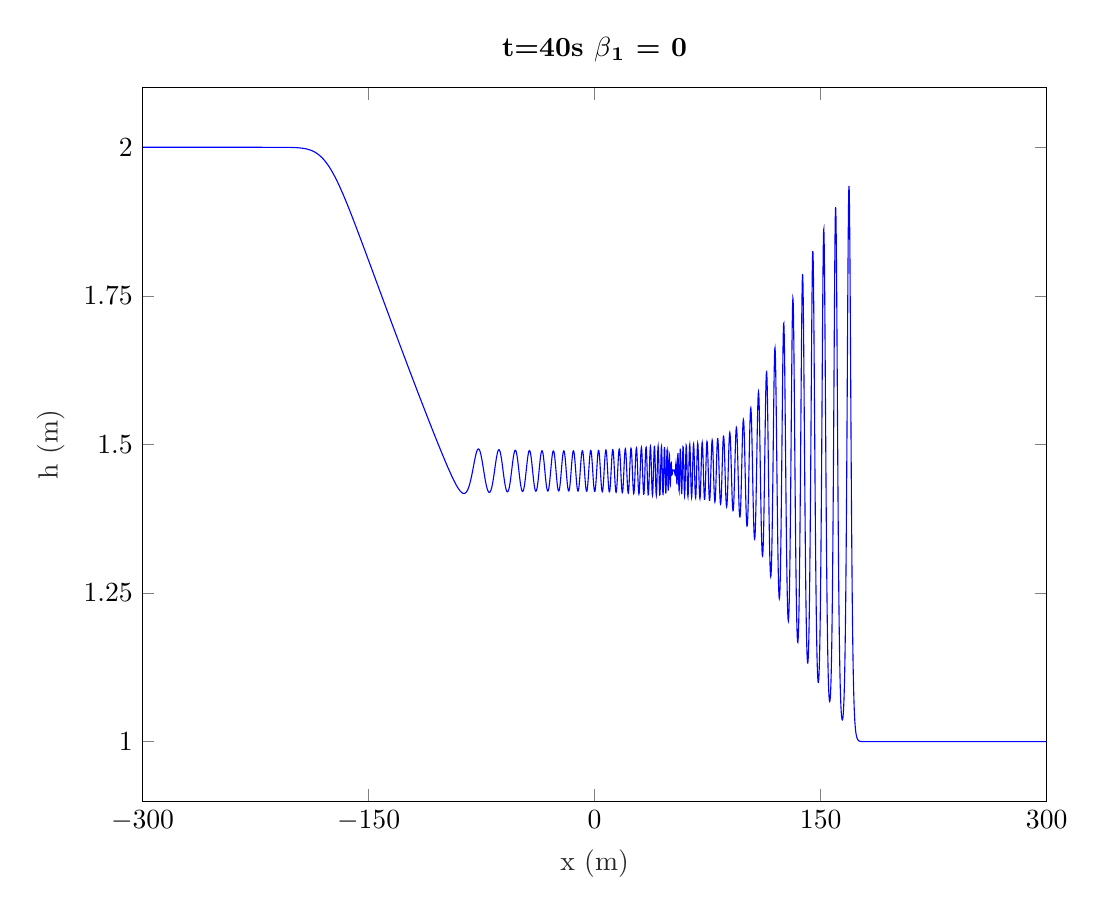
\begin{tikzpicture}

\begin{axis}[%
width=4.521in,
height=3.566in,
at={(0.758in,0.481in)},
scale only axis,
xmin=-300,
xmax=300,
xtick={-300, -150,    0,  150,  300},
xlabel style={font=\color{white!15!black}},
xlabel={x (m)},
ymin=0.9,
ymax=2.1,
ytick={   1, 1.25,  1.5, 1.75,    2},
ylabel style={font=\color{white!15!black}},
ylabel={h (m)},
axis background/.style={fill=white},
title style={font=\bfseries},
title={$\text{t=40s   }\beta{}_\text{1}\text{ = 0}$}
]
\addplot [color=blue, forget plot]
  table[row sep=crcr]{%
-300.18000900045	2\\
-300.030001500075	2\\
-299.8799939997	2\\
-299.729986499325	2\\
-299.57997899895	2\\
-299.429971498575	2\\
-299.2799639982	2\\
-299.129956497825	2\\
-298.97994899745	2\\
-298.829941497075	2\\
-298.6799339967	2\\
-298.529926496325	2\\
-298.37991899595	2\\
-298.229911495575	2\\
-298.0799039952	2\\
-297.929896494825	2\\
-297.77988899445	2\\
-297.629881494075	2\\
-297.4798739937	2\\
-297.329866493325	2\\
-297.17985899295	2\\
-297.029851492575	2\\
-296.8798439922	2\\
-296.729836491825	2\\
-296.57982899145	2\\
-296.429821491075	2\\
-296.2798139907	2\\
-296.129806490325	2\\
-295.979798989949	2\\
-295.829791489574	2\\
-295.679783989199	2\\
-295.529776488824	2\\
-295.379768988449	2\\
-295.229761488074	2\\
-295.079753987699	2\\
-294.929746487324	2\\
-294.779738986949	2\\
-294.629731486574	2\\
-294.479723986199	2\\
-294.329716485824	2\\
-294.179708985449	2\\
-294.029701485074	2\\
-293.879693984699	2\\
-293.729686484324	2\\
-293.579678983949	2\\
-293.429671483574	2\\
-293.279663983199	2\\
-293.129656482824	2\\
-292.979648982449	2\\
-292.829641482074	2\\
-292.679633981699	2\\
-292.529626481324	2\\
-292.379618980949	2\\
-292.229611480574	2\\
-292.079603980199	2\\
-291.929596479824	2\\
-291.779588979449	2\\
-291.629581479074	2\\
-291.479573978699	2\\
-291.329566478324	2\\
-291.179558977949	2\\
-291.029551477574	2\\
-290.879543977199	2\\
-290.729536476824	2\\
-290.579528976449	2\\
-290.429521476074	2\\
-290.279513975699	2\\
-290.129506475324	2\\
-289.979498974949	2\\
-289.829491474574	2\\
-289.679483974199	2\\
-289.529476473824	2\\
-289.379468973449	2\\
-289.229461473074	2\\
-289.079453972699	2\\
-288.929446472324	2\\
-288.779438971949	2\\
-288.629431471574	2\\
-288.479423971199	2\\
-288.329416470824	2\\
-288.179408970449	2\\
-288.029401470073	2\\
-287.879393969698	2\\
-287.729386469323	2\\
-287.579378968948	2\\
-287.429371468573	2\\
-287.279363968198	2\\
-287.129356467823	2\\
-286.979348967448	2\\
-286.829341467073	2\\
-286.679333966698	2\\
-286.529326466323	2\\
-286.379318965948	2\\
-286.229311465573	2\\
-286.079303965198	2\\
-285.929296464823	2\\
-285.779288964448	2\\
-285.629281464073	2\\
-285.479273963698	2\\
-285.329266463323	2\\
-285.179258962948	2\\
-285.029251462573	2\\
-284.879243962198	2\\
-284.729236461823	2\\
-284.579228961448	2\\
-284.429221461073	2\\
-284.279213960698	2\\
-284.129206460323	2\\
-283.979198959948	2\\
-283.829191459573	2\\
-283.679183959198	2\\
-283.529176458823	2\\
-283.379168958448	2\\
-283.229161458073	2\\
-283.079153957698	2\\
-282.929146457323	2\\
-282.779138956948	2\\
-282.629131456573	2\\
-282.479123956198	2\\
-282.329116455823	2\\
-282.179108955448	2\\
-282.029101455073	2\\
-281.879093954698	2\\
-281.729086454323	2\\
-281.579078953948	2\\
-281.429071453573	2\\
-281.279063953198	2\\
-281.129056452823	2\\
-280.979048952448	2\\
-280.829041452073	2\\
-280.679033951698	2\\
-280.529026451323	2\\
-280.379018950948	2\\
-280.229011450573	2\\
-280.079003950197	2\\
-279.928996449822	2\\
-279.778988949447	2\\
-279.628981449072	2\\
-279.478973948697	2\\
-279.328966448322	2\\
-279.178958947947	2\\
-279.028951447572	2\\
-278.878943947197	2\\
-278.728936446822	2\\
-278.578928946447	2\\
-278.428921446072	2\\
-278.278913945697	2\\
-278.128906445322	2\\
-277.978898944947	2\\
-277.828891444572	2\\
-277.678883944197	2\\
-277.528876443822	2\\
-277.378868943447	2\\
-277.228861443072	2\\
-277.078853942697	2\\
-276.928846442322	2\\
-276.778838941947	2\\
-276.628831441572	2\\
-276.478823941197	2\\
-276.328816440822	2\\
-276.178808940447	2\\
-276.028801440072	2\\
-275.878793939697	2\\
-275.728786439322	2\\
-275.578778938947	2\\
-275.428771438572	2\\
-275.278763938197	2\\
-275.128756437822	2\\
-274.978748937447	2\\
-274.828741437072	2\\
-274.678733936697	2\\
-274.528726436322	2\\
-274.378718935947	2\\
-274.228711435572	2\\
-274.078703935197	2\\
-273.928696434822	2\\
-273.778688934447	2\\
-273.628681434072	2\\
-273.478673933697	2\\
-273.328666433322	2\\
-273.178658932947	2\\
-273.028651432572	2\\
-272.878643932197	2\\
-272.728636431822	2\\
-272.578628931447	2\\
-272.428621431072	2\\
-272.278613930697	2\\
-272.128606430321	2\\
-271.978598929946	2\\
-271.828591429571	2\\
-271.678583929196	2\\
-271.528576428821	2\\
-271.378568928446	2\\
-271.228561428071	2\\
-271.078553927696	2\\
-270.928546427321	2\\
-270.778538926946	2\\
-270.628531426571	2\\
-270.478523926196	2\\
-270.328516425821	2\\
-270.178508925446	2\\
-270.028501425071	2\\
-269.878493924696	2\\
-269.728486424321	2\\
-269.578478923946	2\\
-269.428471423571	2\\
-269.278463923196	2\\
-269.128456422821	2\\
-268.978448922446	2\\
-268.828441422071	2\\
-268.678433921696	2\\
-268.528426421321	2\\
-268.378418920946	2\\
-268.228411420571	2\\
-268.078403920196	2\\
-267.928396419821	2\\
-267.778388919446	2\\
-267.628381419071	2\\
-267.478373918696	2\\
-267.328366418321	2\\
-267.178358917946	2\\
-267.028351417571	2\\
-266.878343917196	2\\
-266.728336416821	2\\
-266.578328916446	2\\
-266.428321416071	2\\
-266.278313915696	2\\
-266.128306415321	2\\
-265.978298914946	2\\
-265.828291414571	1.99999999999999\\
-265.678283914196	1.99999999999999\\
-265.528276413821	1.99999999999999\\
-265.378268913446	1.99999999999999\\
-265.228261413071	1.99999999999999\\
-265.078253912696	1.99999999999998\\
-264.928246412321	1.99999999999998\\
-264.778238911946	1.99999999999998\\
-264.628231411571	1.99999999999998\\
-264.478223911196	1.99999999999998\\
-264.328216410821	1.99999999999997\\
-264.178208910446	1.99999999999997\\
-264.02820141007	1.99999999999996\\
-263.878193909695	1.99999999999996\\
-263.72818640932	1.99999999999996\\
-263.578178908945	1.99999999999995\\
-263.42817140857	1.99999999999995\\
-263.278163908195	1.99999999999994\\
-263.12815640782	1.99999999999994\\
-262.978148907445	1.99999999999993\\
-262.82814140707	1.99999999999993\\
-262.678133906695	1.99999999999992\\
-262.52812640632	1.99999999999991\\
-262.378118905945	1.9999999999999\\
-262.22811140557	1.9999999999999\\
-262.078103905195	1.99999999999989\\
-261.92809640482	1.99999999999988\\
-261.778088904445	1.99999999999987\\
-261.62808140407	1.99999999999986\\
-261.478073903695	1.99999999999985\\
-261.32806640332	1.99999999999984\\
-261.178058902945	1.99999999999982\\
-261.02805140257	1.99999999999981\\
-260.878043902195	1.9999999999998\\
-260.72803640182	1.99999999999978\\
-260.578028901445	1.99999999999977\\
-260.42802140107	1.99999999999975\\
-260.278013900695	1.99999999999973\\
-260.12800640032	1.99999999999971\\
-259.977998899945	1.99999999999969\\
-259.82799139957	1.99999999999967\\
-259.677983899195	1.99999999999965\\
-259.52797639882	1.99999999999962\\
-259.377968898445	1.9999999999996\\
-259.22796139807	1.99999999999957\\
-259.077953897695	1.99999999999954\\
-258.92794639732	1.99999999999951\\
-258.777938896945	1.99999999999948\\
-258.62793139657	1.99999999999944\\
-258.477923896195	1.9999999999994\\
-258.32791639582	1.99999999999936\\
-258.177908895445	1.99999999999932\\
-258.02790139507	1.99999999999928\\
-257.877893894695	1.99999999999923\\
-257.72788639432	1.99999999999918\\
-257.577878893945	1.99999999999912\\
-257.42787139357	1.99999999999906\\
-257.277863893195	1.999999999999\\
-257.12785639282	1.99999999999894\\
-256.977848892445	1.99999999999887\\
-256.82784139207	1.99999999999879\\
-256.677833891695	1.99999999999872\\
-256.52782639132	1.99999999999863\\
-256.377818890945	1.99999999999854\\
-256.22781139057	1.99999999999845\\
-256.077803890195	1.99999999999835\\
-255.927796389819	1.99999999999824\\
-255.777788889444	1.99999999999813\\
-255.627781389069	1.99999999999801\\
-255.477773888694	1.99999999999788\\
-255.327766388319	1.99999999999775\\
-255.177758887944	1.9999999999976\\
-255.027751387569	1.99999999999745\\
-254.877743887194	1.99999999999729\\
-254.727736386819	1.99999999999711\\
-254.577728886444	1.99999999999693\\
-254.427721386069	1.99999999999674\\
-254.277713885694	1.99999999999653\\
-254.127706385319	1.99999999999631\\
-253.977698884944	1.99999999999608\\
-253.827691384569	1.99999999999583\\
-253.677683884194	1.99999999999556\\
-253.527676383819	1.99999999999528\\
-253.377668883444	1.99999999999499\\
-253.227661383069	1.99999999999467\\
-253.077653882694	1.99999999999434\\
-252.927646382319	1.99999999999398\\
-252.777638881944	1.9999999999936\\
-252.627631381569	1.9999999999932\\
-252.477623881194	1.99999999999277\\
-252.327616380819	1.99999999999232\\
-252.177608880444	1.99999999999184\\
-252.027601380069	1.99999999999133\\
-251.877593879694	1.99999999999079\\
-251.727586379319	1.99999999999021\\
-251.577578878944	1.9999999999896\\
-251.427571378569	1.99999999998896\\
-251.277563878194	1.99999999998827\\
-251.127556377819	1.99999999998754\\
-250.977548877444	1.99999999998677\\
-250.827541377069	1.99999999998595\\
-250.677533876694	1.99999999998508\\
-250.527526376319	1.99999999998416\\
-250.377518875944	1.99999999998318\\
-250.227511375569	1.99999999998213\\
-250.077503875194	1.99999999998103\\
-249.927496374819	1.99999999997986\\
-249.777488874444	1.99999999997862\\
-249.627481374069	1.9999999999773\\
-249.477473873694	1.99999999997591\\
-249.327466373319	1.99999999997443\\
-249.177458872944	1.99999999997286\\
-249.027451372569	1.99999999997119\\
-248.877443872194	1.99999999996942\\
-248.727436371819	1.99999999996755\\
-248.577428871444	1.99999999996557\\
-248.427421371069	1.99999999996346\\
-248.277413870694	1.99999999996123\\
-248.127406370319	1.99999999995886\\
-247.977398869943	1.99999999995635\\
-247.827391369568	1.99999999995369\\
-247.677383869193	1.99999999995087\\
-247.527376368818	1.99999999994788\\
-247.377368868443	1.99999999994471\\
-247.227361368068	1.99999999994135\\
-247.077353867693	1.99999999993779\\
-246.927346367318	1.99999999993402\\
-246.777338866943	1.99999999993002\\
-246.627331366568	1.99999999992578\\
-246.477323866193	1.99999999992129\\
-246.327316365818	1.99999999991653\\
-246.177308865443	1.99999999991149\\
-246.027301365068	1.99999999990615\\
-245.877293864693	1.99999999990049\\
-245.727286364318	1.9999999998945\\
-245.577278863943	1.99999999988815\\
-245.427271363568	1.99999999988142\\
-245.277263863193	1.9999999998743\\
-245.127256362818	1.99999999986675\\
-244.977248862443	1.99999999985876\\
-244.827241362068	1.99999999985029\\
-244.677233861693	1.99999999984133\\
-244.527226361318	1.99999999983183\\
-244.377218860943	1.99999999982178\\
-244.227211360568	1.99999999981113\\
-244.077203860193	1.99999999979986\\
-243.927196359818	1.99999999978792\\
-243.777188859443	1.99999999977529\\
-243.627181359068	1.99999999976191\\
-243.477173858693	1.99999999974775\\
-243.327166358318	1.99999999973276\\
-243.177158857943	1.9999999997169\\
-243.027151357568	1.9999999997001\\
-242.877143857193	1.99999999968233\\
-242.727136356818	1.99999999966351\\
-242.577128856443	1.9999999996436\\
-242.427121356068	1.99999999962254\\
-242.277113855693	1.99999999960024\\
-242.127106355318	1.99999999957665\\
-241.977098854943	1.99999999955169\\
-241.827091354568	1.99999999952529\\
-241.677083854193	1.99999999949734\\
-241.527076353818	1.99999999946779\\
-241.377068853443	1.99999999943652\\
-241.227061353068	1.99999999940345\\
-241.077053852693	1.99999999936846\\
-240.927046352318	1.99999999933146\\
-240.777038851943	1.99999999929233\\
-240.627031351568	1.99999999925094\\
-240.477023851193	1.99999999920717\\
-240.327016350818	1.99999999916088\\
-240.177008850443	1.99999999911194\\
-240.027001350068	1.99999999906019\\
-239.876993849692	1.99999999900548\\
-239.726986349317	1.99999999894763\\
-239.576978848942	1.99999999888648\\
-239.426971348567	1.99999999882183\\
-239.276963848192	1.99999999875349\\
-239.126956347817	1.99999999868125\\
-238.976948847442	1.9999999986049\\
-238.826941347067	1.99999999852421\\
-238.676933846692	1.99999999843893\\
-238.526926346317	1.9999999983488\\
-238.376918845942	1.99999999825356\\
-238.226911345567	1.99999999815292\\
-238.076903845192	1.99999999804659\\
-237.926896344817	1.99999999793424\\
-237.776888844442	1.99999999781554\\
-237.626881344067	1.99999999769014\\
-237.476873843692	1.99999999755767\\
-237.326866343317	1.99999999741774\\
-237.176858842942	1.99999999726993\\
-237.026851342567	1.99999999711381\\
-236.876843842192	1.99999999694893\\
-236.726836341817	1.9999999967748\\
-236.576828841442	1.99999999659091\\
-236.426821341067	1.99999999639672\\
-236.276813840692	1.99999999619167\\
-236.126806340317	1.99999999597517\\
-235.976798839942	1.99999999574659\\
-235.826791339567	1.99999999550526\\
-235.676783839192	1.9999999952505\\
-235.526776338817	1.99999999498156\\
-235.376768838442	1.99999999469768\\
-235.226761338067	1.99999999439804\\
-235.076753837692	1.99999999408178\\
-234.926746337317	1.99999999374801\\
-234.776738836942	1.99999999339578\\
-234.626731336567	1.99999999302407\\
-234.476723836192	1.99999999263185\\
-234.326716335817	1.99999999221799\\
-234.176708835442	1.99999999178134\\
-234.026701335067	1.99999999132065\\
-233.876693834692	1.99999999083465\\
-233.726686334317	1.99999999032196\\
-233.576678833942	1.99999998978116\\
-233.426671333567	1.99999998921073\\
-233.276663833192	1.99999998860908\\
-233.126656332817	1.99999998797455\\
-232.976648832442	1.99999998730538\\
-232.826641332067	1.99999998659971\\
-232.676633831692	1.9999999858556\\
-232.526626331317	1.99999998507101\\
-232.376618830942	1.99999998424377\\
-232.226611330567	1.99999998337163\\
-232.076603830192	1.99999998245219\\
-231.926596329817	1.99999998148295\\
-231.776588829441	1.99999998046129\\
-231.626581329066	1.99999997938441\\
-231.476573828691	1.99999997824942\\
-231.326566328316	1.99999997705324\\
-231.176558827941	1.99999997579264\\
-231.026551327566	1.99999997446425\\
-230.876543827191	1.99999997306451\\
-230.726536326816	1.99999997158965\\
-230.576528826441	1.99999997003577\\
-230.426521326066	1.9999999683987\\
-230.276513825691	1.99999996667412\\
-230.126506325316	1.99999996485745\\
-229.976498824941	1.99999996294388\\
-229.826491324566	1.99999996092839\\
-229.676483824191	1.99999995880566\\
-229.526476323816	1.99999995657014\\
-229.376468823441	1.99999995421597\\
-229.226461323066	1.99999995173701\\
-229.076453822691	1.99999994912681\\
-228.926446322316	1.99999994637859\\
-228.776438821941	1.99999994348523\\
-228.626431321566	1.99999994043927\\
-228.476423821191	1.99999993723284\\
-228.326416320816	1.99999993385772\\
-228.176408820441	1.99999993030525\\
-228.026401320066	1.99999992656635\\
-227.876393819691	1.99999992263149\\
-227.726386319316	1.99999991849065\\
-227.576378818941	1.99999991413334\\
-227.426371318566	1.99999990954853\\
-227.276363818191	1.99999990472464\\
-227.126356317816	1.99999989964955\\
-226.976348817441	1.99999989431052\\
-226.826341317066	1.99999988869417\\
-226.676333816691	1.99999988278649\\
-226.526326316316	1.99999987657276\\
-226.376318815941	1.99999987003757\\
-226.226311315566	1.99999986316473\\
-226.076303815191	1.99999985593726\\
-225.926296314816	1.99999984833737\\
-225.776288814441	1.99999984034638\\
-225.626281314066	1.99999983194474\\
-225.476273813691	1.99999982311191\\
-225.326266313316	1.99999981382639\\
-225.176258812941	1.99999980406562\\
-225.026251312566	1.99999979380597\\
-224.876243812191	1.99999978302264\\
-224.726236311816	1.99999977168968\\
-224.576228811441	1.99999975977987\\
-224.426221311066	1.99999974726469\\
-224.276213810691	1.99999973411425\\
-224.126206310316	1.99999972029725\\
-223.976198809941	1.99999970578088\\
-223.826191309565	1.99999969053079\\
-223.67618380919	1.99999967451097\\
-223.526176308815	1.99999965768374\\
-223.37616880844	1.9999996400096\\
-223.226161308065	1.99999962144722\\
-223.07615380769	1.99999960195329\\
-222.926146307315	1.99999958148248\\
-222.77613880694	1.99999955998733\\
-222.626131306565	1.99999953741815\\
-222.47612380619	1.99999951372293\\
-222.326116305815	1.99999948884722\\
-222.17610880544	1.99999946273405\\
-222.026101305065	1.99999943532378\\
-221.87609380469	1.99999940655402\\
-221.726086304315	1.99999937635946\\
-221.57607880394	1.99999934467179\\
-221.426071303565	1.99999931141955\\
-221.27606380319	1.99999927652797\\
-221.126056302815	1.99999923991885\\
-220.97604880244	1.99999920151039\\
-220.826041302065	1.99999916121706\\
-220.67603380169	1.99999911894939\\
-220.526026301315	1.99999907461387\\
-220.37601880094	1.9999990281127\\
-220.226011300565	1.99999897934363\\
-220.07600380019	1.99999892819979\\
-219.925996299815	1.99999887456946\\
-219.77598879944	1.99999881833588\\
-219.625981299065	1.99999875937703\\
-219.47597379869	1.99999869756539\\
-219.325966298315	1.99999863276772\\
-219.17595879794	1.99999856484481\\
-219.025951297565	1.99999849365122\\
-218.87594379719	1.99999841903504\\
-218.725936296815	1.99999834083757\\
-218.57592879644	1.99999825889309\\
-218.425921296065	1.99999817302851\\
-218.27591379569	1.9999980830631\\
-218.125906295315	1.99999798880814\\
-217.97589879494	1.99999789006662\\
-217.825891294565	1.99999778663286\\
-217.67588379419	1.99999767829215\\
-217.525876293815	1.99999756482043\\
-217.37586879344	1.99999744598381\\
-217.225861293065	1.99999732153825\\
-217.07585379269	1.99999719122911\\
-216.925846292315	1.99999705479069\\
-216.77583879194	1.99999691194582\\
-216.625831291565	1.99999676240536\\
-216.47582379119	1.99999660586773\\
-216.325816290815	1.99999644201841\\
-216.17580879044	1.9999962705294\\
-216.025801290065	1.99999609105867\\
-215.875793789689	1.99999590324963\\
-215.725786289314	1.99999570673051\\
-215.575778788939	1.99999550111379\\
-215.425771288564	1.99999528599552\\
-215.275763788189	1.99999506095473\\
-215.125756287814	1.99999482555269\\
-214.975748787439	1.99999457933227\\
-214.825741287064	1.99999432181718\\
-214.675733786689	1.99999405251123\\
-214.525726286314	1.99999377089753\\
-214.375718785939	1.99999347643772\\
-214.225711285564	1.99999316857111\\
-214.075703785189	1.99999284671382\\
-213.925696284814	1.9999925102579\\
-213.775688784439	1.99999215857036\\
-213.625681284064	1.99999179099228\\
-213.475673783689	1.99999140683774\\
-213.325666283314	1.99999100539286\\
-213.175658782939	1.99999058591471\\
-213.025651282564	1.99999014763018\\
-212.875643782189	1.99998968973491\\
-212.725636281814	1.99998921139206\\
-212.575628781439	1.99998871173113\\
-212.425621281064	1.99998818984667\\
-212.275613780689	1.99998764479703\\
-212.125606280314	1.99998707560298\\
-211.975598779939	1.99998648124632\\
-211.825591279564	1.99998586066851\\
-211.675583779189	1.99998521276911\\
-211.525576278814	1.99998453640432\\
-211.375568778439	1.99998383038537\\
-211.225561278064	1.99998309347692\\
-211.075553777689	1.99998232439536\\
-210.925546277314	1.99998152180708\\
-210.775538776939	1.99998068432671\\
-210.625531276564	1.99997981051524\\
-210.475523776189	1.99997889887818\\
-210.325516275814	1.99997794786351\\
-210.175508775439	1.99997695585978\\
-210.025501275064	1.99997592119392\\
-209.875493774689	1.99997484212916\\
-209.725486274314	1.99997371686281\\
-209.575478773939	1.99997254352398\\
-209.425471273564	1.99997132017125\\
-209.275463773189	1.99997004479023\\
-209.125456272814	1.99996871529111\\
-208.975448772439	1.99996732950609\\
-208.825441272064	1.99996588518678\\
-208.675433771689	1.99996438000142\\
-208.525426271314	1.9999628115322\\
-208.375418770939	1.99996117727234\\
-208.225411270564	1.99995947462315\\
-208.075403770189	1.99995770089104\\
-207.925396269813	1.99995585328439\\
-207.775388769438	1.99995392891039\\
-207.625381269063	1.99995192477172\\
-207.475373768688	1.99994983776322\\
-207.325366268313	1.99994766466846\\
-207.175358767938	1.99994540215614\\
-207.025351267563	1.9999430467765\\
-206.875343767188	1.99994059495758\\
-206.725336266813	1.99993804300137\\
-206.575328766438	1.99993538707994\\
-206.425321266063	1.99993262323138\\
-206.275313765688	1.99992974735571\\
-206.125306265313	1.99992675521065\\
-205.975298764938	1.99992364240728\\
-205.825291264563	1.99992040440565\\
-205.675283764188	1.99991703651025\\
-205.525276263813	1.99991353386536\\
-205.375268763438	1.99990989145032\\
-205.225261263063	1.99990610407467\\
-205.075253762688	1.99990216637325\\
-204.925246262313	1.99989807280104\\
-204.775238761938	1.9998938176281\\
-204.625231261563	1.99988939493418\\
-204.475223761188	1.9998847986034\\
-204.325216260813	1.99988002231873\\
-204.175208760438	1.99987505955632\\
-204.025201260063	1.99986990357985\\
-203.875193759688	1.99986454743462\\
-203.725186259313	1.99985898394161\\
-203.575178758938	1.99985320569145\\
-203.425171258563	1.99984720503818\\
-203.275163758188	1.99984097409299\\
-203.125156257813	1.9998345047178\\
-202.975148757438	1.99982778851878\\
-202.825141257063	1.99982081683967\\
-202.675133756688	1.99981358075508\\
-202.525126256313	1.99980607106361\\
-202.375118755938	1.99979827828096\\
-202.225111255563	1.99979019263281\\
-202.075103755188	1.99978180404769\\
-201.925096254813	1.99977310214971\\
-201.775088754438	1.9997640762512\\
-201.625081254063	1.99975471534524\\
-201.475073753688	1.99974500809812\\
-201.325066253313	1.99973494284167\\
-201.175058752938	1.99972450756554\\
-201.025051252563	1.99971368990934\\
-200.875043752188	1.9997024771548\\
-200.725036251813	1.9996908562177\\
-200.575028751438	1.99967881363986\\
-200.425021251063	1.999666335581\\
-200.275013750688	1.99965340781053\\
-200.125006250313	1.99964001569927\\
-199.974998749937	1.99962614421117\\
-199.824991249562	1.99961177789491\\
-199.674983749187	1.9995969008755\\
-199.524976248812	1.9995814968458\\
-199.374968748437	1.99956554905807\\
-199.224961248062	1.99954904031543\\
-199.074953747687	1.99953195296334\\
-198.924946247312	1.99951426888102\\
-198.774938746937	1.99949596947295\\
-198.624931246562	1.99947703566031\\
-198.474923746187	1.99945744787241\\
-198.324916245812	1.99943718603823\\
-198.174908745437	1.9994162295779\\
-198.024901245062	1.99939455739428\\
-197.874893744687	1.99937214786457\\
-197.724886244312	1.99934897883195\\
-197.574878743937	1.99932502759736\\
-197.424871243562	1.99930027091128\\
-197.274863743187	1.99927468496568\\
-197.124856242812	1.99924824538602\\
-196.974848742437	1.99922092722339\\
-196.824841242062	1.99919270494676\\
-196.674833741687	1.99916355243541\\
-196.524826241312	1.99913344297151\\
-196.374818740937	1.99910234923279\\
-196.224811240562	1.99907024328552\\
-196.074803740187	1.9990370965776\\
-195.924796239812	1.99900287993187\\
-195.774788739437	1.99896756353969\\
-195.624781239062	1.99893111695472\\
-195.474773738687	1.99889350908697\\
-195.324766238312	1.99885470819713\\
-195.174758737937	1.99881468189119\\
-195.024751237562	1.99877339711535\\
-194.874743737187	1.99873082015129\\
-194.724736236812	1.99868691661171\\
-194.574728736437	1.99864165143632\\
-194.424721236062	1.99859498888813\\
-194.274713735687	1.99854689255014\\
-194.124706235312	1.9984973253225\\
-193.974698734937	1.99844624941999\\
-193.824691234562	1.99839362637006\\
-193.674683734187	1.99833941701126\\
-193.524676233812	1.99828358149215\\
-193.374668733437	1.99822607927075\\
-193.224661233062	1.99816686911446\\
-193.074653732687	1.99810590910056\\
-192.924646232312	1.99804315661722\\
-192.774638731937	1.99797856836508\\
-192.624631231562	1.99791210035947\\
-192.474623731187	1.99784370793317\\
-192.324616230812	1.99777334573981\\
-192.174608730437	1.99770096775796\\
-192.024601230062	1.99762652729575\\
-191.874593729686	1.99754997699632\\
-191.724586229311	1.9974712688438\\
-191.574578728936	1.99739035417015\\
-191.424571228561	1.99730718366253\\
-191.274563728186	1.9972217073716\\
-191.124556227811	1.99713387472039\\
-190.974548727436	1.99704363451405\\
-190.824541227061	1.99695093495029\\
-190.674533726686	1.99685572363066\\
-190.524526226311	1.99675794757256\\
-190.374518725936	1.99665755322212\\
-190.224511225561	1.99655448646785\\
-190.074503725186	1.99644869265509\\
-189.924496224811	1.99634011660134\\
-189.774488724436	1.99622870261239\\
-189.624481224061	1.99611439449931\\
-189.474473723686	1.99599713559622\\
-189.324466223311	1.99587686877901\\
-189.174458722936	1.99575353648481\\
-189.024451222561	1.99562708073238\\
-188.874443722186	1.99549744314329\\
-188.724436221811	1.99536456496398\\
-188.574428721436	1.99522838708867\\
-188.424421221061	1.99508885008308\\
-188.274413720686	1.99494589420897\\
-188.124406220311	1.99479945944959\\
-187.974398719936	1.99464948553582\\
-187.824391219561	1.9944959119732\\
-187.674383719186	1.99433867806974\\
-187.524376218811	1.9941777229645\\
-187.374368718436	1.99401298565689\\
-187.224361218061	1.99384440503683\\
-187.074353717686	1.9936719199155\\
-186.924346217311	1.9934954690569\\
-186.774338716936	1.99331499121005\\
-186.624331216561	1.99313042514189\\
-186.474323716186	1.99294170967075\\
-186.324316215811	1.99274878370051\\
-186.174308715436	1.99255158625529\\
-186.024301215061	1.99235005651474\\
-185.874293714686	1.99214413384978\\
-185.724286214311	1.99193375785894\\
-185.574278713936	1.99171886840503\\
-185.424271213561	1.99149940565233\\
-185.274263713186	1.99127531010412\\
-185.124256212811	1.99104652264057\\
-184.974248712436	1.99081298455688\\
-184.824241212061	1.99057463760178\\
-184.674233711686	1.99033142401616\\
-184.524226211311	1.99008328657194\\
-184.374218710936	1.98983016861103\\
-184.224211210561	1.98957201408439\\
-184.074203710186	1.98930876759114\\
-183.92419620981	1.98904037441765\\
-183.774188709435	1.98876678057654\\
-183.62418120906	1.98848793284568\\
-183.474173708685	1.98820377880687\\
-183.32416620831	1.98791426688448\\
-183.174158707935	1.98761934638371\\
-183.02415120756	1.98731896752856\\
-182.874143707185	1.98701308149953\\
-182.72413620681	1.98670164047078\\
-182.574128706435	1.98638459764689\\
-182.42412120606	1.98606190729912\\
-182.274113705685	1.98573352480102\\
-182.12410620531	1.98539940666354\\
-181.974098704935	1.98505951056934\\
-181.82409120456	1.98471379540646\\
-181.674083704185	1.98436222130123\\
-181.52407620381	1.98400474965024\\
-181.374068703435	1.9836413431516\\
-181.22406120306	1.98327196583517\\
-181.074053702685	1.98289658309185\\
-180.92404620231	1.98251516170192\\
-180.774038701935	1.9821276698622\\
-180.62403120156	1.98173407721224\\
-180.474023701185	1.98133435485933\\
-180.32401620081	1.98092847540229\\
-180.174008700435	1.9805164129541\\
-180.02400120006	1.98009814316329\\
-179.873993699685	1.97967364323394\\
-179.72398619931	1.97924289194451\\
-179.573978698935	1.97880586966521\\
-179.42397119856	1.97836255837405\\
-179.273963698185	1.97791294167149\\
-179.12395619781	1.97745700479358\\
-178.973948697435	1.97699473462381\\
-178.82394119706	1.97652611970334\\
-178.673933696685	1.97605115023985\\
-178.52392619631	1.97556981811483\\
-178.373918695935	1.97508211688941\\
-178.22391119556	1.97458804180866\\
-178.073903695185	1.97408758980432\\
-177.92389619481	1.97358075949609\\
-177.773888694435	1.97306755119129\\
-177.62388119406	1.97254796688312\\
-177.473873693685	1.97202201024726\\
-177.32386619331	1.97148968663702\\
-177.173858692935	1.97095100307702\\
-177.02385119256	1.9704059682553\\
-176.873843692185	1.96985459251398\\
-176.72383619181	1.96929688783847\\
-176.573828691435	1.9687328678452\\
-176.42382119106	1.96816254776795\\
-176.273813690685	1.96758594444276\\
-176.123806190309	1.96700307629147\\
-175.973798689934	1.96641396330394\\
-175.823791189559	1.96581862701891\\
-175.673783689184	1.96521709050357\\
-175.523776188809	1.96460937833194\\
-175.373768688434	1.96399551656196\\
-175.223761188059	1.96337553271145\\
-175.073753687684	1.96274945573295\\
-174.923746187309	1.96211731598736\\
-174.773738686934	1.96147914521668\\
-174.623731186559	1.9608349765156\\
-174.473723686184	1.96018484430224\\
-174.323716185809	1.95952878428784\\
-174.173708685434	1.95886683344574\\
-174.023701185059	1.9581990299794\\
-173.873693684684	1.95752541328973\\
-173.723686184309	1.95684602394166\\
-173.573678683934	1.95616090363004\\
-173.423671183559	1.95547009514496\\
-173.273663683184	1.95477364233643\\
-173.123656182809	1.95407159007861\\
-172.973648682434	1.95336398423355\\
-172.823641182059	1.9526508716145\\
-172.673633681684	1.95193229994887\\
-172.523626181309	1.95120831784089\\
-172.373618680934	1.95047897473404\\
-172.223611180559	1.94974432087317\\
-172.073603680184	1.9490044072666\\
-171.923596179809	1.94825928564803\\
-171.773588679434	1.94750900843835\\
-171.623581179059	1.94675362870761\\
-171.473573678684	1.94599320013683\\
-171.323566178309	1.94522777698003\\
-171.173558677934	1.94445741402634\\
-171.023551177559	1.94368216656229\\
-170.873543677184	1.94290209033433\\
-170.723536176809	1.94211724151161\\
-170.573528676434	1.94132767664906\\
-170.423521176059	1.94053345265081\\
-170.273513675684	1.93973462673397\\
-170.123506175309	1.9389312563929\\
-169.973498674934	1.93812339936385\\
-169.823491174559	1.93731111359014\\
-169.673483674184	1.93649445718781\\
-169.523476173809	1.93567348841188\\
-169.373468673434	1.93484826562314\\
-169.223461173059	1.93401884725558\\
-169.073453672684	1.93318529178442\\
-168.923446172309	1.93234765769482\\
-168.773438671934	1.93150600345126\\
-168.623431171559	1.9306603874676\\
-168.473423671184	1.9298108680779\\
-168.323416170809	1.92895750350798\\
-168.173408670434	1.92810035184762\\
-168.023401170058	1.92723947102369\\
-167.873393669683	1.92637491877395\\
-167.723386169308	1.92550675262169\\
-167.573378668933	1.92463502985109\\
-167.423371168558	1.92375980748354\\
-167.273363668183	1.92288114225459\\
-167.123356167808	1.92199909059186\\
-166.973348667433	1.92111370859373\\
-166.823341167058	1.92022505200882\\
-166.673333666683	1.91933317621631\\
-166.523326166308	1.91843813620718\\
-166.373318665933	1.91753998656608\\
-166.223311165558	1.91663878145422\\
-166.073303665183	1.91573457459296\\
-165.923296164808	1.91482741924826\\
-165.773288664433	1.91391736821588\\
-165.623281164058	1.91300447380745\\
-165.473273663683	1.91208878783732\\
-165.323266163308	1.91117036161011\\
-165.173258662933	1.91024924590912\\
-165.023251162558	1.90932549098547\\
-164.873243662183	1.90839914654801\\
-164.723236161808	1.90747026175388\\
-164.573228661433	1.90653888519993\\
-164.423221161058	1.90560506491472\\
-164.273213660683	1.90466884835129\\
-164.123206160308	1.90373028238061\\
-163.973198659933	1.90278941328562\\
-163.823191159558	1.90184628675605\\
-163.673183659183	1.90090094788373\\
-163.523176158808	1.89995344115861\\
-163.373168658433	1.89900381046535\\
-163.223161158058	1.8980520990805\\
-163.073153657683	1.89709834967021\\
-162.923146157308	1.89614260428858\\
-162.773138656933	1.89518490437639\\
-162.623131156558	1.89422529076053\\
-162.473123656183	1.89326380365372\\
-162.323116155808	1.8923004826549\\
-162.173108655433	1.89133536674994\\
-162.023101155058	1.89036849431286\\
-161.873093654683	1.88939990310745\\
-161.723086154308	1.8884296302893\\
-161.573078653933	1.88745771240823\\
-161.423071153558	1.88648418541108\\
-161.273063653183	1.88550908464485\\
-161.123056152808	1.88453244486019\\
-160.973048652433	1.8835543002152\\
-160.823041152058	1.88257468427955\\
-160.673033651683	1.88159363003885\\
-160.523026151308	1.88061116989935\\
-160.373018650933	1.87962733569286\\
-160.223011150558	1.87864215868189\\
-160.073003650182	1.87765566956507\\
-159.922996149807	1.87666789848275\\
-159.772988649432	1.87567887502277\\
-159.622981149057	1.8746886282265\\
-159.472973648682	1.87369718659494\\
-159.322966148307	1.87270457809504\\
-159.172958647932	1.87171083016618\\
-159.022951147557	1.87071596972672\\
-158.872943647182	1.8697200231807\\
-158.722936146807	1.86872301642466\\
-158.572928646432	1.86772497485456\\
-158.422921146057	1.86672592337271\\
-158.272913645682	1.86572588639487\\
-158.122906145307	1.86472488785738\\
-157.972898644932	1.86372295122428\\
-157.822891144557	1.86272009949461\\
-157.672883644182	1.86171635520959\\
-157.522876143807	1.86071174045991\\
-157.372868643432	1.85970627689309\\
-157.222861143057	1.85869998572069\\
-157.072853642682	1.85769288772569\\
-156.922846142307	1.85668500326978\\
-156.772838641932	1.85567635230059\\
-156.622831141557	1.85466695435906\\
-156.472823641182	1.85365682858659\\
-156.322816140807	1.85264599373232\\
-156.172808640432	1.85163446816027\\
-156.022801140057	1.85062226985651\\
-155.872793639682	1.84960941643619\\
-155.722786139307	1.84859592515064\\
-155.572778638932	1.8475818128943\\
-155.422771138557	1.84656709621169\\
-155.272763638182	1.84555179130421\\
-155.122756137807	1.84453591403696\\
-154.972748637432	1.84351947994546\\
-154.822741137057	1.8425025042423\\
-154.672733636682	1.84148500182365\\
-154.522726136307	1.84046698727584\\
-154.372718635932	1.83944847488168\\
-154.222711135557	1.83842947862682\\
-154.072703635182	1.83741001220602\\
-153.922696134807	1.83639008902921\\
-153.772688634432	1.83536972222766\\
-153.622681134057	1.83434892465984\\
-153.472673633682	1.8333277089174\\
-153.322666133307	1.83230608733087\\
-153.172658632932	1.83128407197543\\
-153.022651132557	1.83026167467645\\
-152.872643632182	1.82923890701503\\
-152.722636131807	1.8282157803334\\
-152.572628631432	1.82719230574022\\
-152.422621131057	1.82616849411585\\
-152.272613630682	1.82514435611741\\
-152.122606130307	1.82411990218387\\
-151.972598629931	1.82309514254095\\
-151.822591129556	1.82207008720598\\
-151.672583629181	1.82104474599266\\
-151.522576128806	1.82001912851567\\
-151.372568628431	1.81899324419528\\
-151.222561128056	1.81796710226181\\
-151.072553627681	1.81694071176\\
-150.922546127306	1.81591408155328\\
-150.772538626931	1.81488722032802\\
-150.622531126556	1.8138601365976\\
-150.472523626181	1.81283283870645\\
-150.322516125806	1.81180533483398\\
-150.172508625431	1.81077763299842\\
-150.022501125056	1.8097497410606\\
-149.872493624681	1.80872166672765\\
-149.722486124306	1.80769341755656\\
-149.572478623931	1.80666500095773\\
-149.422471123556	1.80563642419839\\
-149.272463623181	1.80460769440598\\
-149.122456122806	1.80357881857142\\
-148.972448622431	1.80254980355231\\
-148.822441122056	1.8015206560761\\
-148.672433621681	1.8004913827431\\
-148.522426121306	1.79946199002952\\
-148.372418620931	1.79843248429032\\
-148.222411120556	1.79740287176214\\
-148.072403620181	1.79637315856601\\
-147.922396119806	1.7953433507101\\
-147.772388619431	1.79431345409236\\
-147.622381119056	1.79328347450309\\
-147.472373618681	1.7922534176275\\
-147.322366118306	1.7912232890481\\
-147.172358617931	1.79019309424719\\
-147.022351117556	1.78916283860912\\
-146.872343617181	1.7881325274226\\
-146.722336116806	1.78710216588296\\
-146.572328616431	1.78607175909428\\
-146.422321116056	1.78504131207153\\
-146.272313615681	1.7840108297426\\
-146.122306115306	1.78298031695039\\
-145.972298614931	1.78194977845469\\
-145.822291114556	1.78091921893414\\
-145.672283614181	1.77988864298811\\
-145.522276113806	1.77885805513847\\
-145.372268613431	1.77782745983143\\
-145.222261113056	1.77679686143922\\
-145.072253612681	1.77576626426181\\
-144.922246112306	1.77473567252852\\
-144.772238611931	1.77370509039967\\
-144.622231111556	1.77267452196812\\
-144.472223611181	1.77164397126081\\
-144.322216110806	1.77061344224021\\
-144.172208610431	1.76958293880583\\
-144.022201110056	1.76855246479559\\
-143.87219360968	1.7675220239872\\
-143.722186109305	1.76649162009955\\
-143.57217860893	1.76546125679397\\
-143.422171108555	1.76443093767555\\
-143.27216360818	1.76340066629434\\
-143.122156107805	1.76237044614662\\
-142.97214860743	1.76134028067607\\
-142.822141107055	1.76031017327491\\
-142.67213360668	1.75928012728505\\
-142.522126106305	1.75825014599918\\
-142.37211860593	1.75722023266187\\
-142.222111105555	1.7561903904706\\
-142.07210360518	1.75516062257677\\
-141.922096104805	1.75413093208674\\
-141.77208860443	1.75310132206277\\
-141.622081104055	1.75207179552398\\
-141.47207360368	1.75104235544731\\
-141.322066103305	1.75001300476839\\
-141.17205860293	1.74898374638246\\
-141.022051102555	1.74795458314517\\
-140.87204360218	1.74692551787354\\
-140.722036101805	1.74589655334667\\
-140.57202860143	1.74486769230662\\
-140.422021101055	1.74383893745916\\
-140.27201360068	1.74281029147457\\
-140.122006100305	1.74178175698838\\
-139.97199859993	1.74075333660209\\
-139.821991099555	1.73972503288391\\
-139.67198359918	1.73869684836947\\
-139.521976098805	1.73766878556247\\
-139.37196859843	1.7366408469354\\
-139.221961098055	1.73561303493016\\
-139.07195359768	1.73458535195874\\
-138.921946097305	1.7335578004038\\
-138.77193859693	1.73253038261933\\
-138.621931096555	1.73150310093125\\
-138.47192359618	1.73047595763796\\
-138.321916095805	1.72944895501097\\
-138.17190859543	1.72842209529543\\
-138.021901095055	1.72739538071069\\
-137.87189359468	1.72636881345088\\
-137.721886094305	1.72534239568537\\
-137.57187859393	1.72431612955936\\
-137.421871093555	1.72329001719437\\
-137.27186359318	1.7222640606887\\
-137.121856092805	1.721238262118\\
-136.97184859243	1.72021262353568\\
-136.821841092055	1.71918714697342\\
-136.67183359168	1.71816183444161\\
-136.521826091305	1.71713668792985\\
-136.37181859093	1.71611170940734\\
-136.221811090555	1.71508690082337\\
-136.07180359018	1.7140622641077\\
-135.921796089805	1.71303780117103\\
-135.771788589429	1.71201351390539\\
-135.621781089054	1.71098940418453\\
-135.471773588679	1.70996547386439\\
-135.321766088304	1.70894172478343\\
-135.171758587929	1.70791815876302\\
-135.021751087554	1.70689477760788\\
-134.871743587179	1.70587158310639\\
-134.721736086804	1.70484857703099\\
-134.571728586429	1.70382576113856\\
-134.421721086054	1.70280313717073\\
-134.271713585679	1.70178070685431\\
-134.121706085304	1.70075847190155\\
-133.971698584929	1.69973643401055\\
-133.821691084554	1.69871459486556\\
-133.671683584179	1.69769295613736\\
-133.521676083804	1.69667151948352\\
-133.371668583429	1.69565028654879\\
-133.221661083054	1.69462925896539\\
-133.071653582679	1.69360843835332\\
-132.921646082304	1.69258782632071\\
-132.771638581929	1.69156742446408\\
-132.621631081554	1.69054723436869\\
-132.471623581179	1.68952725760882\\
-132.321616080804	1.68850749574805\\
-132.171608580429	1.68748795033961\\
-132.021601080054	1.68646862292662\\
-131.871593579679	1.68544951504242\\
-131.721586079304	1.68443062821083\\
-131.571578578929	1.68341196394644\\
-131.421571078554	1.6823935237549\\
-131.271563578179	1.68137530913322\\
-131.121556077804	1.68035732156999\\
-130.971548577429	1.67933956254571\\
-130.821541077054	1.67832203353305\\
-130.671533576679	1.6773047359971\\
-130.521526076304	1.67628767139569\\
-130.371518575929	1.67527084117958\\
-130.221511075554	1.67425424679282\\
-130.071503575179	1.67323788967294\\
-129.921496074804	1.67222177125126\\
-129.771488574429	1.67120589295314\\
-129.621481074054	1.67019025619824\\
-129.471473573679	1.66917486240077\\
-129.321466073304	1.66815971296977\\
-129.171458572929	1.66714480930939\\
-129.021451072554	1.66613015281908\\
-128.871443572179	1.66511574489395\\
-128.721436071804	1.66410158692492\\
-128.571428571429	1.66308768029906\\
-128.421421071054	1.66207402639983\\
-128.271413570679	1.66106062660731\\
-128.121406070304	1.66004748229849\\
-127.971398569929	1.65903459484753\\
-127.821391069553	1.65802196562599\\
-127.671383569178	1.65700959600313\\
-127.521376068803	1.65599748734613\\
-127.371368568428	1.65498564102041\\
-127.221361068053	1.65397405838981\\
-127.071353567678	1.65296274081695\\
-126.921346067303	1.6519516896634\\
-126.771338566928	1.65094090629002\\
-126.621331066553	1.64993039205721\\
-126.471323566178	1.64892014832515\\
-126.321316065803	1.64791017645408\\
-126.171308565428	1.64690047780462\\
-126.021301065053	1.64589105373799\\
-125.871293564678	1.64488190561631\\
-125.721286064303	1.64387303480287\\
-125.571278563928	1.64286444266242\\
-125.421271063553	1.64185613056145\\
-125.271263563178	1.64084809986849\\
-125.121256062803	1.63984035195437\\
-124.971248562428	1.63883288819256\\
-124.821241062053	1.63782570995941\\
-124.671233561678	1.63681881863449\\
-124.521226061303	1.63581221560088\\
-124.371218560928	1.63480590224546\\
-124.221211060553	1.63379987995927\\
-124.071203560178	1.63279415013774\\
-123.921196059803	1.63178871418112\\
-123.771188559428	1.63078357349469\\
-123.621181059053	1.62977872948916\\
-123.471173558678	1.628774183581\\
-123.321166058303	1.62776993719272\\
-123.171158557928	1.62676599175328\\
-123.021151057553	1.62576234869841\\
-122.871143557178	1.62475900947093\\
-122.721136056803	1.62375597552118\\
-122.571128556428	1.62275324830731\\
-122.421121056053	1.62175082929573\\
-122.271113555678	1.62074871996141\\
-122.121106055303	1.6197469217883\\
-121.971098554928	1.61874543626976\\
-121.821091054553	1.61774426490887\\
-121.671083554178	1.61674340921892\\
-121.521076053803	1.6157428707238\\
-121.371068553428	1.61474265095837\\
-121.221061053053	1.613742751469\\
-121.071053552678	1.61274317381388\\
-120.921046052303	1.61174391956358\\
-120.771038551928	1.61074499030145\\
-120.621031051553	1.60974638762408\\
-120.471023551178	1.60874811314184\\
-120.321016050803	1.60775016847929\\
-120.171008550428	1.60675255527574\\
-120.021001050052	1.6057552751857\\
-119.870993549677	1.60475832987949\\
-119.720986049302	1.60376172104369\\
-119.570978548927	1.60276545038172\\
-119.420971048552	1.6017695196144\\
-119.270963548177	1.60077393048053\\
-119.120956047802	1.59977868473746\\
-118.970948547427	1.59878378416169\\
-118.820941047052	1.5977892305495\\
-118.670933546677	1.59679502571758\\
-118.520926046302	1.59580117150365\\
-118.370918545927	1.59480766976716\\
-118.220911045552	1.59381452238993\\
-118.070903545177	1.59282173127689\\
-117.920896044802	1.59182929835677\\
-117.770888544427	1.59083722558281\\
-117.620881044052	1.58984551493357\\
-117.470873543677	1.58885416841368\\
-117.320866043302	1.5878631880546\\
-117.170858542927	1.58687257591547\\
-117.020851042552	1.58588233408397\\
-116.870843542177	1.58489246467711\\
-116.720836041802	1.5839029698422\\
-116.570828541427	1.5829138517577\\
-116.420821041052	1.58192511263417\\
-116.270813540677	1.58093675471524\\
-116.120806040302	1.57994878027861\\
-115.970798539927	1.57896119163703\\
-115.820791039552	1.5779739911394\\
-115.670783539177	1.57698718117181\\
-115.520776038802	1.57600076415867\\
-115.370768538427	1.57501474256382\\
-115.220761038052	1.57402911889176\\
-115.070753537677	1.57304389568884\\
-114.920746037302	1.57205907554447\\
-114.770738536927	1.57107466109248\\
-114.620731036552	1.57009065501239\\
-114.470723536177	1.56910706003081\\
-114.320716035802	1.56812387892281\\
-114.170708535427	1.56714111451343\\
-114.020701035052	1.56615876967913\\
-113.870693534677	1.56517684734938\\
-113.720686034302	1.5641953505082\\
-113.570678533927	1.56321428219586\\
-113.420671033552	1.56223364551055\\
-113.270663533177	1.56125344361015\\
-113.120656032802	1.56027367971403\\
-112.970648532427	1.55929435710492\\
-112.820641032052	1.55831547913084\\
-112.670633531677	1.5573370492071\\
-112.520626031302	1.55635907081838\\
-112.370618530927	1.55538154752081\\
-112.220611030552	1.55440448294421\\
-112.070603530176	1.55342788079437\\
-111.920596029801	1.55245174485536\\
-111.770588529426	1.55147607899202\\
-111.620581029051	1.55050088715243\\
-111.470573528676	1.54952617337051\\
-111.320566028301	1.54855194176876\\
-111.170558527926	1.54757819656097\\
-111.020551027551	1.54660494205517\\
-110.870543527176	1.5456321826566\\
-110.720536026801	1.54465992287073\\
-110.570528526426	1.54368816730656\\
-110.420521026051	1.54271692067986\\
-110.270513525676	1.54174618781662\\
-110.120506025301	1.54077597365658\\
-109.970498524926	1.53980628325697\\
-109.820491024551	1.53883712179624\\
-109.670483524176	1.53786849457809\\
-109.520476023801	1.53690040703552\\
-109.370468523426	1.53593286473508\\
-109.220461023051	1.53496587338127\\
-109.070453522676	1.53399943882116\\
-108.920446022301	1.53303356704903\\
-108.770438521926	1.5320682642114\\
-108.620431021551	1.53110353661201\\
-108.470423521176	1.53013939071722\\
-108.320416020801	1.52917583316143\\
-108.170408520426	1.52821287075279\\
-108.020401020051	1.52725051047917\\
-107.870393519676	1.52628875951425\\
-107.720386019301	1.52532762522393\\
-107.570378518926	1.52436711517295\\
-107.420371018551	1.52340723713182\\
-107.270363518176	1.52244799908392\\
-107.120356017801	1.52148940923297\\
-106.970348517426	1.5205314760108\\
-106.820341017051	1.51957420808532\\
-106.670333516676	1.51861761436895\\
-106.520326016301	1.51766170402727\\
-106.370318515926	1.51670648648808\\
-106.220311015551	1.51575197145081\\
-106.070303515176	1.51479816889632\\
-105.920296014801	1.51384508909707\\
-105.770288514426	1.51289274262773\\
-105.620281014051	1.51194114037622\\
-105.470273513676	1.5109902935552\\
-105.320266013301	1.51004021371403\\
-105.170258512926	1.50909091275126\\
-105.020251012551	1.50814240292756\\
-104.870243512176	1.50719469687929\\
-104.720236011801	1.50624780763258\\
-104.570228511426	1.505301748618\\
-104.420221011051	1.50435653368589\\
-104.270213510676	1.50341217712228\\
-104.120206010301	1.50246869366556\\
-103.970198509925	1.50152609852381\\
-103.82019100955	1.5005844073929\\
-103.670183509175	1.49964363647535\\
-103.5201760088	1.49870380250003\\
-103.370168508425	1.49776492274268\\
-103.22016100805	1.49682701504739\\
-103.070153507675	1.49589009784892\\
-102.9201460073	1.4949541901961\\
-102.770138506925	1.4940193117762\\
-102.62013100655	1.49308548294038\\
-102.470123506175	1.49215272473028\\
-102.3201160058	1.49122105890582\\
-102.170108505425	1.49029050797421\\
-102.02010100505	1.48936109522021\\
-101.870093504675	1.48843284473789\\
-101.7200860043	1.48750578146364\\
-101.570078503925	1.48657993121085\\
-101.42007100355	1.48565532070602\\
-101.270063503175	1.48473197762662\\
-101.1200560028	1.48380993064058\\
-100.970048502425	1.48288920944766\\
-100.82004100205	1.48196984482271\\
-100.670033501675	1.48105186866089\\
-100.5200260013	1.48013531402498\\
-100.370018500925	1.47922021519491\\
-100.22001100055	1.47830660771958\\
-100.070003500175	1.47739452847104\\
-99.9199959998	1.47648401570128\\
-99.769988499425	1.47557510910159\\
-99.6199809990499	1.47466784986477\\
-99.4699734986749	1.47376228075023\\
-99.3199659982999	1.47285844615212\\
-99.1699584979249	1.47195639217074\\
-99.0199509975499	1.47105616668728\\
-98.8699434971749	1.47015781944209\\
-98.7199359967998	1.4692614021167\\
-98.5699284964248	1.46836696841967\\
-98.4199209960498	1.46747457417664\\
-98.2699134956748	1.46658427742447\\
-98.1199059952998	1.46569613851013\\
-97.9698984949247	1.46481022019405\\
-97.8198909945497	1.46392658775859\\
-97.6698834941747	1.46304530912165\\
-97.5198759937997	1.46216645495565\\
-97.3698684934247	1.46129009881232\\
-97.2198609930497	1.46041631725336\\
-97.0698534926746	1.45954518998746\\
-96.9198459922996	1.45867680001382\\
-96.7698384919246	1.45781123377255\\
-96.6198309915496	1.45694858130233\\
-96.4698234911746	1.45608893640553\\
-96.3198159907996	1.45523239682133\\
-96.1698084904245	1.45437906440703\\
-96.0198009900495	1.45352904532806\\
-95.8697934896745	1.45268245025703\\
-95.7197859892995	1.45183939458223\\
-95.5697784889244	1.45099999862608\\
-95.4197709885494	1.45016438787385\\
-95.2697634881744	1.44933269321326\\
-95.1197559877994	1.44850505118532\\
-94.9697484874244	1.44768160424688\\
-94.8197409870494	1.44686250104557\\
-94.6697334866743	1.44604789670741\\
-94.5197259862993	1.4452379531378\\
-94.3697184859243	1.44443283933636\\
-94.2197109855493	1.44363273172612\\
-94.0697034851743	1.44283781449775\\
-93.9196959847992	1.44204827996931\\
-93.7696884844242	1.44126432896203\\
-93.6196809840492	1.44048617119285\\
-93.4696734836742	1.4397140256842\\
-93.3196659832992	1.43894812119157\\
-93.1696584829241	1.43818869664948\\
-93.0196509825491	1.43743600163636\\
-92.8696434821741	1.43669029685891\\
-92.7196359817991	1.43595185465641\\
-92.5696284814241	1.43522095952547\\
-92.4196209810491	1.43449790866562\\
-92.269613480674	1.43378301254616\\
-92.119605980299	1.43307659549462\\
-91.969598479924	1.43237899630698\\
-91.819590979549	1.43169056887991\\
-91.669583479174	1.43101168286513\\
-91.5195759787989	1.43034272434575\\
-91.3695684784239	1.42968409653443\\
-91.2195609780489	1.42903622049314\\
-91.0695534776739	1.42839953587393\\
-90.9195459772989	1.42777450167996\\
-90.7695384769239	1.42716159704601\\
-90.6195309765488	1.42656132203717\\
-90.4695234761738	1.42597419846425\\
-90.3195159757988	1.4254007707141\\
-90.1695084754238	1.42484160659274\\
-90.0195009750487	1.42429729817861\\
-89.8694934746737	1.42376846268296\\
-89.7194859742987	1.4232557433138\\
-89.5694784739237	1.42275981013921\\
-89.4194709735487	1.42228136094544\\
-89.2694634731737	1.42182112208403\\
-89.1194559727986	1.42137984930205\\
-88.9694484724236	1.42095832854803\\
-88.8194409720486	1.42055737674593\\
-88.6694334716736	1.42017784252769\\
-88.5194259712986	1.41982060691461\\
-88.3694184709235	1.41948658393591\\
-88.2194109705485	1.41917672117192\\
-88.0694034701735	1.41889200020778\\
-87.9193959697985	1.41863343698196\\
-87.7693884694235	1.41840208201251\\
-87.6193809690484	1.41819902048172\\
-87.4693734686734	1.41802537215857\\
-87.3193659682984	1.41788229113599\\
-87.1693584679234	1.41777096535791\\
-87.0193509675484	1.41769261591065\\
-86.8693434671734	1.41764850462836\\
-86.7193359667984	1.4176400476105\\
-86.5693284664233	1.41766811588484\\
-86.4193209660483	1.41773450255975\\
-86.2693134656733	1.41784042595913\\
-86.1193059652983	1.41798727085879\\
-85.9692984649232	1.41817644255753\\
-85.8192909645482	1.41840936315885\\
-85.6692834641732	1.41868746497754\\
-85.5192759637982	1.41901218483993\\
-85.3692684634232	1.41938495924718\\
-85.2192609630482	1.41980721814391\\
-85.0692534626731	1.42028037705674\\
-84.9192459622981	1.42080582898704\\
-84.7692384619231	1.4213849355908\\
-84.6192309615481	1.42201901712149\\
-84.4692234611731	1.42270934137112\\
-84.319215960798	1.42345711174706\\
-84.169208460423	1.42426345423854\\
-84.019200960048	1.4251294032483\\
-83.869193459673	1.4260558863635\\
-83.719185959298	1.42704370801727\\
-83.5691784589229	1.42809353206017\\
-83.4191709585479	1.42920586325121\\
-83.2691634581729	1.43038102773428\\
-83.1191559577979	1.43161915256312\\
-82.9691484574229	1.43292014436385\\
-82.8191409570479	1.43428366725469\\
-82.6691334566728	1.43570912017619\\
-82.5191259562978	1.43719561381467\\
-82.3691184559228	1.43874194733594\\
-82.2191109555478	1.44034658518416\\
-82.0691034551728	1.44200763424031\\
-81.9190959547977	1.44372282167291\\
-81.7690884544227	1.44548947385124\\
-81.6190809540477	1.44730449673157\\
-81.4690734536727	1.44916435816169\\
-81.3190659532977	1.45106507258035\\
-81.1690584529227	1.45300218861633\\
-81.0190509525476	1.45497078010994\\
-80.8690434521726	1.45696544109665\\
-80.7190359517976	1.45898028528988\\
-80.5690284514226	1.46100895058538\\
-80.4190209510475	1.463044609103\\
-80.2690134506725	1.46507998322066\\
-80.1190059502975	1.46710736801732\\
-79.9689984499225	1.4691186604651\\
-79.8189909495475	1.4711053956159\\
-79.6689834491725	1.47305878992904\\
-79.5189759487974	1.47496979175807\\
-79.3689684484224	1.47682913887793\\
-79.2189609480474	1.47862742278542\\
-79.0689534476724	1.48035515933966\\
-78.9189459472974	1.48200286514262\\
-78.7689384469223	1.48356113890287\\
-78.6189309465473	1.48502074684449\\
-78.4689234461723	1.48637271107904\\
-78.3189159457973	1.48760839971914\\
-78.1689084454223	1.48871961738386\\
-78.0189009450472	1.48969869466421\\
-77.8688934446722	1.49053857504989\\
-77.7188859442972	1.4912328977948\\
-77.5688784439222	1.49177607521263\\
-77.4188709435472	1.49216336295498\\
-77.2688634431722	1.49239089955936\\
-77.1188559427972	1.49245504284941\\
-76.9688484424221	1.49235630500319\\
-76.8188409420471	1.49209140260141\\
-76.6688334416721	1.49166134867968\\
-76.5188259412971	1.49106740019012\\
-76.368818440922	1.4903118281649\\
-76.218810940547	1.48939796866726\\
-76.068803440172	1.48833012789902\\
-75.918795939797	1.48711357282342\\
-75.768788439422	1.48575446974254\\
-75.618780939047	1.48425981968187\\
-75.4687734386719	1.4826373950238\\
-75.3187659382969	1.48089564446624\\
-75.1687584379219	1.47904364671863\\
-75.0187509375469	1.47709098156176\\
-74.8687434371719	1.47504766657296\\
-74.7187359367968	1.47292408598897\\
-74.5687284364218	1.47073084969171\\
-74.4187209360468	1.46847876452994\\
-74.2687134356718	1.46617873140823\\
-74.1187059352968	1.46384164203086\\
-73.9686984349217	1.46147835670403\\
-73.8186909345467	1.45909960171209\\
-73.6686834341717	1.45671591298261\\
-73.5186759337967	1.45433760502638\\
-73.3686684334217	1.45197470197425\\
-73.2186609330467	1.44963691129171\\
-73.0686534326716	1.44733358849434\\
-72.9186459322966	1.44507371467569\\
-72.7686384319216	1.44286588099244\\
-72.6186309315466	1.44071826123495\\
-72.4686234311716	1.43863862857037\\
-72.3186159307965	1.43663434093207\\
-72.1686084304215	1.43471232928607\\
-72.0186009300465	1.43287913606284\\
-71.8685934296715	1.43114090156756\\
-71.7185859292965	1.42950336672366\\
-71.5685784289215	1.42797191582653\\
-71.4185709285464	1.4265515677805\\
-71.2685634281714	1.42524698646615\\
-71.1185559277964	1.42406251506634\\
-70.9685484274214	1.4230021735516\\
-70.8185409270463	1.42206967055399\\
-70.6685334266713	1.42126842021806\\
-70.5185259262963	1.42060154391433\\
-70.3685184259213	1.42007187957184\\
-70.2185109255463	1.41968197648836\\
-70.0685034251713	1.41943409432357\\
-69.9184959247962	1.41932909417114\\
-69.7684884244212	1.41937204062879\\
-69.6184809240462	1.41956081720936\\
-69.4684734236712	1.41989765514251\\
-69.3184659232962	1.42038318840295\\
-69.1684584229211	1.42101768479186\\
-69.0184509225461	1.42180100829302\\
-68.8684434221711	1.42273256518197\\
-68.7184359217961	1.4238112638981\\
-68.5684284214211	1.42503548620572\\
-68.418420921046	1.42640303040907\\
-68.268413420671	1.42791106101618\\
-68.118405920296	1.42955606436367\\
-67.968398419921	1.43133379349347\\
-67.818390919546	1.43323921963549\\
-67.668383419171	1.4352664791012\\
-67.518375918796	1.43740882410899\\
-67.3683684184209	1.43965859022286\\
-67.2183609180459	1.44200715047493\\
-67.0683534176709	1.44444488068423\\
-66.9183459172959	1.44696115457428\\
-66.7683384169208	1.44954432773537\\
-66.6183309165458	1.45218173161095\\
-66.4683234161708	1.45485970799101\\
-66.3183159157958	1.45756364350485\\
-66.1683084154208	1.46027801090897\\
-66.0183009150458	1.46298645303786\\
-65.8682934146707	1.46567187868691\\
-65.7182859142957	1.46831656952518\\
-65.5682784139207	1.47090231928062\\
-65.4182709135457	1.47341058945828\\
-65.2682634131707	1.47582268446085\\
-65.1182559127956	1.47811994550367\\
-64.9682484124206	1.48028395045727\\
-64.8182409120456	1.48229673739303\\
-64.6682334116706	1.48414103687034\\
-64.5182259112956	1.48580048913511\\
-64.3682184109205	1.48725987573152\\
-64.2182109105455	1.48850535457837\\
-64.0682034101705	1.48952465930832\\
-63.9181959097955	1.49030729080911\\
-63.7681884094205	1.49084470359629\\
-63.6181809090455	1.49113051637022\\
-63.4681734086704	1.49115902212371\\
-63.3181659082954	1.49093222238647\\
-63.1681584079204	1.49044676575711\\
-63.0181509075454	1.48970662381428\\
-62.8681434071704	1.48871693733823\\
-62.7181359067953	1.48748506949476\\
-62.5681284064203	1.48602058527466\\
-62.4181209060453	1.48433512206346\\
-62.2681134056703	1.4824421908279\\
-62.1181059052953	1.48035703463073\\
-61.9680984049203	1.47809641716248\\
-61.8180909045452	1.47567842517839\\
-61.6680834041702	1.47312218799659\\
-61.5180759037952	1.47044773962987\\
-61.3680684034202	1.4676757197206\\
-61.2180609030451	1.46482716072528\\
-61.0680534026701	1.46192333523674\\
-60.9180459022951	1.4589854517856\\
-60.7680384019201	1.45603457682941\\
-60.6180309015451	1.453091401187\\
-60.4680234011701	1.45017609076744\\
-60.318015900795	1.44730821362844\\
-60.16800840042	1.44450656002266\\
-60.018000900045	1.44178910159017\\
-59.86799339967	1.43917290297061\\
-59.717985899295	1.43667405912915\\
-59.5679783989199	1.43430766940219\\
-59.4179708985449	1.43208781562914\\
-59.2679633981699	1.43002752030592\\
-59.1179558977949	1.42813876370412\\
-58.9679483974199	1.42643249238615\\
-58.8179408970448	1.42491858203323\\
-58.6679333966698	1.42360589616003\\
-58.5179258962948	1.42250224839339\\
-58.3679183959198	1.42161442911204\\
-58.2179108955448	1.42094821593568\\
-58.0679033951698	1.4205083301792\\
-57.9178958947948	1.42029741021451\\
-57.7678883944197	1.42032164250047\\
-57.6178808940447	1.4205783310412\\
-57.4678733936697	1.42106996284879\\
-57.3178658932947	1.42179549750657\\
-57.1678583929196	1.42275295860837\\
-57.0178508925446	1.423939110333\\
-56.8678433921696	1.42534939388941\\
-56.7178358917946	1.42697783175435\\
-56.5678283914196	1.42881696723721\\
-56.4178208910446	1.43085779786703\\
-56.2678133906695	1.43308971204435\\
-56.1178058902945	1.43550040989833\\
-55.9677983899195	1.43807587296784\\
-55.8177908895445	1.44080031404594\\
-55.6677833891695	1.44365616687992\\
-55.5177758887944	1.44662409197411\\
-55.3677683884194	1.44968299561256\\
-55.2177608880444	1.45281011242014\\
-55.0677533876694	1.45598108925414\\
-54.9177458872944	1.45917013131998\\
-54.7677383869193	1.46235018180872\\
-54.6177308865443	1.46549313619326\\
-54.4677233861693	1.46857010912927\\
-54.3177158857943	1.47155173407156\\
-54.1677083854193	1.47440851686427\\
-54.0177008850443	1.47711120527951\\
-53.8676933846692	1.4796311900879\\
-53.7176858842942	1.4819409341969\\
-53.5676783839192	1.48401440413026\\
-53.4176708835442	1.48582750674599\\
-53.2676633831692	1.48735850522592\\
-53.1176558827941	1.48858842587556\\
-52.9676483824191	1.48950141927255\\
-52.8176408820441	1.49008508458293\\
-52.6676333816691	1.49033373264791\\
-52.5176258812941	1.49023335430841\\
-52.3676183809191	1.48979254448296\\
-52.217610880544	1.48901135040559\\
-52.067603380169	1.48789717511845\\
-51.917595879794	1.48646130300366\\
-51.767588379419	1.48471878003977\\
-51.6175808790439	1.48268816826025\\
-51.4675733786689	1.48039124557031\\
-51.3175658782939	1.47785265355744\\
-51.1675583779189	1.47509950308859\\
-51.0175508775439	1.47216095202726\\
-50.8675433771689	1.46906777543447\\
-50.7175358767938	1.46585193073275\\
-50.5675283764188	1.46254612917957\\
-50.4175208760438	1.45918341735659\\
-50.2675133756688	1.45579678857405\\
-50.1175058752938	1.45241883042884\\
-49.9674983749187	1.44908140151014\\
-49.8174908745437	1.44581534447265\\
-49.6674833741687	1.44265023997893\\
-49.5174758737937	1.43961420362523\\
-49.3674683734187	1.43673371963161\\
-49.2174608730436	1.43403350452091\\
-49.0674533726686	1.43153640107307\\
-48.9174458722936	1.42926330061432\\
-48.7674383719186	1.42723308819928\\
-48.6174308715436	1.42546260314898\\
-48.4674233711686	1.42396660893495\\
-48.3174158707936	1.42275776620273\\
-48.1674083704185	1.42184661197804\\
-48.0174008700435	1.4212415409813\\
-47.8673933696685	1.42094749208854\\
-47.7173858692935	1.42097289473542\\
-47.5673783689184	1.42131400745858\\
-47.4173708685434	1.42197315237063\\
-47.2673633681684	1.42294686219778\\
-47.1173558677934	1.42422975549359\\
-46.9673483674184	1.42581390494709\\
-46.8173408670434	1.42768876758397\\
-46.6673333666683	1.42984110191647\\
-46.5173258662933	1.43225489906972\\
-46.3673183659183	1.43491131824857\\
-46.2173108655433	1.43778864588601\\
-46.0673033651683	1.44086229006545\\
-45.9172958647932	1.44410481776953\\
-45.7672883644182	1.44748602729939\\
-45.6172808640432	1.45097307205815\\
-45.4672733636682	1.45453066300529\\
-45.3172658632932	1.45812133055646\\
-45.1672583629181	1.46170575951336\\
-45.0172508625431	1.46524319517458\\
-44.8672433621681	1.46869192594195\\
-44.7172358617931	1.47200984207727\\
-44.5672283614181	1.47515505289449\\
-44.4172208610431	1.47808654845439\\
-44.267213360668	1.48076490670851\\
-44.117205860293	1.48315302165486\\
-43.967198359918	1.48521682566236\\
-43.817190859543	1.48692598935115\\
-43.667183359168	1.4882545806629\\
-43.5171758587929	1.48918165241595\\
-43.3671683584179	1.48969158480536\\
-43.2171608580429	1.48977290148321\\
-43.0671533576679	1.48942857482581\\
-42.9171458572928	1.48865476051888\\
-42.7671383569178	1.48746276285337\\
-42.6171308565428	1.48586775906715\\
-42.4671233561678	1.48389074322656\\
-42.3171158557928	1.48155814316022\\
-42.1671083554178	1.47890127962406\\
-42.0171008550428	1.47595579191004\\
-41.8670933546678	1.47276096114786\\
-41.7170858542927	1.46935899012014\\
-41.5670783539177	1.46579428063304\\
-41.4170708535427	1.46211268694623\\
-41.2670633531677	1.45836082012589\\
-41.1170558527926	1.45458534976569\\
-40.9670483524176	1.45083239515125\\
-40.8170408520426	1.44714693936374\\
-40.6670333516676	1.44357234286797\\
-40.5170258512925	1.44014989985122\\
-40.3670183509175	1.43691847980417\\
-40.2170108505425	1.43391421951766\\
-40.0670033501675	1.4311702836843\\
-39.9169958497925	1.42871667470589\\
-39.7669883494175	1.42658007934058\\
-39.6169808490425	1.42478375052884\\
-39.4669733486674	1.42334741795758\\
-39.3169658482924	1.42228721214245\\
-39.1669583479174	1.42161558547181\\
-39.0169508475424	1.42133797334237\\
-38.8669433471674	1.42146926723512\\
-38.7169358467924	1.42200039319515\\
-38.5669283464173	1.42293181175759\\
-38.4169208460423	1.42425647020902\\
-38.2669133456673	1.42596318327076\\
-38.1169058452923	1.42803651101786\\
-37.9668983449172	1.43045668214813\\
-37.8168908445422	1.43319953454545\\
-37.6668833441672	1.4362365001306\\
-37.5168758437922	1.43953463020314\\
-37.3668683434172	1.44305667877546\\
-37.2168608430421	1.44676127848085\\
-37.0668533426671	1.45060319089837\\
-36.9168458422921	1.45453367791078\\
-36.7668383419171	1.45850097327644\\
-36.6168308415421	1.46245087856502\\
-36.4668233411671	1.4663274846225\\
-36.3168158407921	1.47007400803364\\
-36.166808340417	1.47363372890077\\
-36.016800840042	1.47695102663325\\
-35.866793339667	1.47997246985731\\
-35.716785839292	1.48264794968993\\
-35.5667783389169	1.484931806572\\
-35.4167708385419	1.48678391630102\\
-35.2667633381669	1.48817069504838\\
-35.1167558377919	1.48906599113877\\
-34.9667483374168	1.4894568297642\\
-34.8167408370418	1.48931841850127\\
-34.6667333366668	1.48866628125641\\
-34.5167258362918	1.48750359412279\\
-34.3667183359168	1.48584815115309\\
-34.2167108355418	1.48372624109219\\
-34.0667033351668	1.4811720877645\\
-33.9166958347918	1.47822714245711\\
-33.7666883344167	1.47493913438705\\
-33.6166808340417	1.47136103446962\\
-33.4666733336667	1.46754994349631\\
-33.3166658332917	1.46356593398056\\
-33.1666583329167	1.45947090323777\\
-33.0166508325416	1.45532745930678\\
-32.8666433321666	1.45119788368045\\
-32.7166358317916	1.44714314712005\\
-32.5666283314166	1.44322209132668\\
-32.4166208310415	1.43949062225297\\
-32.2666133306665	1.43600114417413\\
-32.1166058302915	1.43280194816728\\
-31.9665983299165	1.42993685774871\\
-31.8165908295415	1.42744481224685\\
-31.6665833291665	1.4253596379691\\
-31.5165758287914	1.42370979913942\\
-31.3665683284164	1.42251823125789\\
-31.2165608280414	1.42180220972573\\
-31.0665533276664	1.42157422026724\\
-30.9165458272914	1.42183656324023\\
-30.7665383269164	1.42259185598266\\
-30.6165308265414	1.4238322325236\\
-30.4665233261663	1.42554465419104\\
-30.3165158257913	1.42770966866189\\
-30.1665083254163	1.43030133657836\\
-30.0165008250412	1.43328726224539\\
-29.8664933246662	1.43662856957167\\
-29.7164858242912	1.44028006995151\\
-29.5664783239162	1.44419049430831\\
-29.4164708235412	1.44830284789087\\
-29.2664633231661	1.45255494989437\\
-29.1164558227911	1.45688012786864\\
-28.9664483224161	1.46120811926328\\
-28.8164408220411	1.46546611339931\\
-28.6664333216661	1.4695800441956\\
-28.5164258212911	1.47347599633039\\
-28.3664183209161	1.47708174763447\\
-28.216410820541	1.48032845044986\\
-28.066403320166	1.48315229204515\\
-27.916395819791	1.48549616512263\\
-27.766388319416	1.48731126876683\\
-27.616380819041	1.48855850193379\\
-27.4663733186659	1.48921055440215\\
-27.3163658182909	1.48924564724906\\
-27.1663583179159	1.48867061450669\\
-27.0163508175409	1.48748528883249\\
-26.8663433171658	1.48571349149352\\
-26.7163358167908	1.48338841737807\\
-26.5663283164158	1.48055442220786\\
-26.4163208160408	1.47726584779942\\
-26.2663133156658	1.47358563873218\\
-26.1163058152908	1.46958380693086\\
-25.9662983149157	1.46533570484989\\
-25.8162908145407	1.46092029905879\\
-25.6662833141657	1.45641849577336\\
-25.5162758137907	1.45191146583023\\
-25.3662683134157	1.44747908816404\\
-25.2162608130407	1.44319863701259\\
-25.0662533126657	1.43914354256353\\
-24.9162458122906	1.43538229889355\\
-24.7662383119156	1.43197763134977\\
-24.6162308115406	1.42898580700099\\
-24.4662233111655	1.42645598687469\\
-24.3162158107905	1.4244297988917\\
-24.1662083104155	1.42294098065726\\
-24.0162008100405	1.42201503337445\\
-23.8661933096655	1.42166593366897\\
-23.7161858092904	1.42191174033956\\
-23.5661783089154	1.42274181246371\\
-23.4161708085404	1.42415047497664\\
-23.2661633081654	1.42611888741407\\
-23.1161558077904	1.42861916015002\\
-22.9661483074154	1.43161421635382\\
-22.8161408070404	1.4350577166764\\
-22.6661333066654	1.43889441666382\\
-22.5161258062903	1.44306044350285\\
-22.3661183059153	1.44748388789125\\
-22.2161108055403	1.45208562113353\\
-22.0661033051653	1.45678035011456\\
-21.9160958047902	1.46147795943672\\
-21.7660883044152	1.46608516607254\\
-21.6160808040402	1.47050741868213\\
-21.4660733036652	1.47465101160442\\
-21.3160658032901	1.47842542872702\\
-21.1660583029151	1.48174575513245\\
-21.0160508025401	1.48453513525623\\
-20.8660433021651	1.48672711270087\\
-20.7160358017901	1.4882677656062\\
-20.5660283014151	1.48911728361929\\
-20.4160208010401	1.48924839945628\\
-20.266013300665	1.48866619861741\\
-20.11600580029	1.48736840066271\\
-19.965998299915	1.48538635205308\\
-19.81599079954	1.48276338554016\\
-19.665983299165	1.4795578153931\\
-19.51597579879	1.47584119213854\\
-19.3659682984149	1.47169623878175\\
-19.2159607980399	1.46721453484287\\
-19.0659532976649	1.46249402337267\\
-18.9159457972899	1.45763648540293\\
-18.7659382969148	1.45274510504459\\
-18.6159307965398	1.4479221217505\\
-18.4659232961648	1.44326671705927\\
-18.3159157957898	1.43887313598297\\
-18.1659082954148	1.43482905293757\\
-18.0159007950397	1.43121420022854\\
-17.8658932946647	1.42809925305014\\
-17.7158857942897	1.42554492127116\\
-17.5658782939147	1.42360121527613\\
-17.4158707935397	1.42230687474406\\
-17.2658632931647	1.42168461995362\\
-17.1158557927897	1.4217637339614\\
-16.9658482924146	1.42252962741885\\
-16.8158407920396	1.42398053245043\\
-16.6658332916646	1.42609220888447\\
-16.5158257912896	1.42882888815235\\
-16.3658182909145	1.4321419706412\\
-16.2158107905395	1.4359702773109\\
-16.0658032901645	1.44024045625037\\
-15.9157957897895	1.44486771777161\\
-15.7657882894144	1.44975686588352\\
-15.6157807890394	1.45480368675348\\
-15.4657732886644	1.45989680636692\\
-15.3157657882894	1.46491992038569\\
-15.1657582879144	1.46975444420247\\
-15.0157507875394	1.47428252926882\\
-14.8657432871644	1.47839032920795\\
-14.7157357867894	1.4819714627597\\
-14.5657282864143	1.48493045736591\\
-14.4157207860393	1.48718606501265\\
-14.2657132856643	1.48867426654581\\
-14.1157057852893	1.48935955687364\\
-13.9656982849143	1.4891912974112\\
-13.8156907845392	1.48819907224315\\
-13.6656832841642	1.48639371916734\\
-13.5156757837892	1.48382089975259\\
-13.3656682834142	1.48054615220039\\
-13.2156607830391	1.47665361573273\\
-13.0656532826641	1.47224323287686\\
-12.9156457822891	1.46742753538204\\
-12.7656382819141	1.46232815914741\\
-12.6156307815391	1.45707227137396\\
-12.4656232811641	1.45178903780367\\
-12.315615780789	1.44660626631958\\
-12.165608280414	1.44164738426266\\
-12.015600780039	1.43702873855808\\
-11.865593279664	1.43285728123533\\
-11.715585779289	1.42922863383321\\
-11.565578278914	1.42622553072247\\
-11.4155707785389	1.42391654439401\\
-11.2655632781639	1.42235511301672\\
-11.1155557777889	1.42157554722106\\
-10.9655482774139	1.42161047599265\\
-10.8155407770388	1.42244847921534\\
-10.6655332766638	1.42408503906788\\
-10.5155257762888	1.42648752130828\\
-10.3655182759138	1.4296075886132\\
-10.2155107755388	1.43337957290835\\
-10.0655032751637	1.4377210303835\\
-9.91549577478872	1.44253352676322\\
-9.76548827441371	1.44770402155269\\
-9.6154807740387	1.45310667844756\\
-9.46547327366369	1.45860537084588\\
-9.31546577328868	1.46405659920955\\
-9.16545827291367	1.46931333349877\\
-9.0154507725386	1.47422903463128\\
-8.86544327216359	1.4786622789744\\
-8.71543577178858	1.48248171159416\\
-8.56542827141357	1.48557069563524\\
-8.41542077103855	1.48783198265154\\
-8.26541327066354	1.4891915704144\\
-8.11540577028853	1.48959749938493\\
-7.96539826991352	1.48904693621688\\
-7.81539076953845	1.48753608003716\\
-7.66538326916344	1.48511178787492\\
-7.51537576878843	1.48184399038743\\
-7.36536826841342	1.47782843378402\\
-7.21536076803841	1.47318305533336\\
-7.0653532676634	1.46804368523857\\
-6.91534576728839	1.46255925221022\\
-6.76533826691332	1.45688677767765\\
-6.61533076653831	1.45118634697763\\
-6.4653232661633	1.44561639667451\\
-6.31531576578828	1.44032938767056\\
-6.16530826541327	1.4354679797325\\
-6.01530076503826	1.43116178533596\\
-5.86529326466325	1.42752467972459\\
-5.71528576428824	1.42465262337401\\
-5.56527826391317	1.42262194014282\\
-5.41527076353816	1.42148843974027\\
-5.26526326316315	1.42128969220248\\
-5.11525576278814	1.42202120534039\\
-4.96524826241313	1.42368620345198\\
-4.81524076203812	1.4262431167206\\
-4.6652332616631	1.42963224265007\\
-4.51522576128809	1.43377087568275\\
-4.36521826091303	1.43855396764757\\
-4.21521076053801	1.44385554142799\\
-4.065203260163	1.44953095281619\\
-3.91519575978799	1.45541975849162\\
-3.76518825941298	1.46134948620135\\
-3.61518075903797	1.46714028683875\\
-3.46517325866296	1.47261060867884\\
-3.31516575828789	1.47758324299154\\
-3.16515825791288	1.48189199474996\\
-3.01515075753787	1.485388419053\\
-2.86514325716286	1.48794824958063\\
-2.71513575678784	1.48947673956396\\
-2.56512825641283	1.48990795904369\\
-2.41512075603782	1.48924005880624\\
-2.26511325566281	1.48746969238143\\
-2.11510575528774	1.48465952347685\\
-1.96509825491273	1.48090216571819\\
-1.81509075453772	1.47632290999073\\
-1.66508325416271	1.47107455357669\\
-1.5150757537877	1.46533119037569\\
-1.36506825341269	1.45928141960506\\
-1.21506075303768	1.45312131207546\\
-1.06505325266261	1.44704757017863\\
-0.915045752287597	1.44125127705864\\
-0.765038251912586	1.43591218512236\\
-0.615030751537574	1.43119382941858\\
-0.465023251162563	1.42723955634383\\
-0.315015750787552	1.42416925089237\\
-0.165008250412541	1.42207675853854\\
-0.0150007500375295	1.42102336235833\\
0.135006750337539	1.42106229384188\\
0.28501425071255	1.42217705311479\\
0.435021751087561	1.42435548380489\\
0.585029251462572	1.42753836075053\\
0.735036751837583	1.43163831458778\\
0.885044252212595	1.43653785468634\\
1.03505175258761	1.4420911802462\\
1.18505925296267	1.44812685638023\\
1.33506675333768	1.45445168468589\\
1.4850742537127	1.46085578961963\\
1.63508175408771	1.46711898876434\\
1.78508925446272	1.47301836456054\\
1.93509675483773	1.47833686145165\\
2.08510425521274	1.48287243383798\\
2.23511175558775	1.48644724912934\\
2.38511925596282	1.48891645857492\\
2.53512675633783	1.49018181306445\\
2.68513425671284	1.49016322054977\\
2.83514175708785	1.48888274882463\\
2.98514925746287	1.48636626844136\\
3.13515675783788	1.48270986017092\\
3.28516425821289	1.47805112390611\\
3.43517175858796	1.47256617781825\\
3.58517925896297	1.4664617419494\\
3.73518675933798	1.4599657433066\\
3.88519425971299	1.4533177940717\\
4.035201760088	1.44675959804196\\
4.18520926046301	1.44052606735775\\
4.33521676083802	1.43483739641863\\
4.48522426121303	1.42989222590496\\
4.6352317615881	1.42586202137103\\
4.78523926196311	1.42288662923645\\
4.93524676233812	1.42107088029077\\
5.08525426271314	1.42048549461057\\
5.23526176308815	1.42114647265784\\
5.38526926346316	1.42305216924256\\
5.53527676383817	1.42614383442475\\
5.68528426421324	1.43032600601546\\
5.83529176458825	1.4354631254552\\
5.98529926496326	1.44138193019825\\
6.13530676533827	1.44787511377608\\
6.28531426571328	1.45470664676951\\
6.43532176608829	1.46161882900684\\
6.5853292664633	1.46834124247346\\
6.73533676683832	1.47460142863283\\
6.88534426721338	1.48013686059735\\
7.03535176758839	1.48470757379612\\
7.18535926796341	1.48810887683483\\
7.33536676833842	1.490182307464\\
7.48537426871343	1.4908187092817\\
7.63538176908844	1.49000299525348\\
7.78538926946345	1.48773813613896\\
7.93539676983852	1.48412449658106\\
8.08540427021353	1.47931493875789\\
8.23541177058854	1.47351485127891\\
8.38541927096355	1.46697155416579\\
8.53542677133856	1.45996183680112\\
8.68543427171358	1.4527786933595\\
8.83544177208859	1.44571812557466\\
8.9854492724636	1.43906685545855\\
9.13545677283867	1.43309136124548\\
9.28546427321368	1.428028574003\\
9.43547177358869	1.42407826975561\\
9.5854792739637	1.42139718784626\\
9.73548677433871	1.42008343267407\\
9.88549427471372	1.42023285857082\\
10.0355017750887	1.42180544214345\\
10.1855092754638	1.42477513381085\\
10.3355167758388	1.42903521338482\\
10.4855242762138	1.43442998285374\\
10.6355317765888	1.44075373519667\\
10.7855392769638	1.44775570193968\\
10.9355467773389	1.45514731269122\\
11.0855542777139	1.46261207509774\\
11.2355617780889	1.46981811545614\\
11.3855692784639	1.47643315223836\\
11.535576778839	1.4821412288108\\
11.685584279214	1.48666020837358\\
11.835591779589	1.4897587681618\\
11.985599279964	1.49128764062045\\
12.135606780339	1.49110373694394\\
12.285614280714	1.48926732138469\\
12.435621781089	1.48582910676037\\
12.5856292814641	1.48095635328135\\
12.7356367818391	1.47488350436171\\
12.8856442822141	1.46790323387428\\
13.0356517825891	1.46034971392491\\
13.1856592829641	1.45258043285792\\
13.3356667833391	1.44495806461183\\
13.4856742837142	1.43783323658001\\
13.6356817840892	1.43152945105994\\
13.7856892844642	1.42633029220378\\
13.9356967848393	1.42246907938902\\
14.0857042852143	1.42012142922358\\
14.2357117855893	1.41940733602761\\
14.3857192859643	1.42034240525875\\
14.5357267863393	1.4229269288239\\
14.6857342867143	1.42705348584243\\
14.8357417870894	1.4325533107656\\
14.9857492874644	1.43919107981675\\
15.1357567878394	1.44667063704846\\
15.2857642882144	1.45464469087282\\
15.4357717885894	1.46272795553375\\
15.5857792889644	1.470514184151\\
15.7357867893394	1.47759697054481\\
15.8857942897145	1.48359276244573\\
16.0358017900895	1.48816498525223\\
16.1858092904645	1.49104683528677\\
16.3358167908395	1.4920624946865\\
16.4858242912146	1.49113549892189\\
16.6358317915896	1.48830699619797\\
16.7858392919646	1.48372333217413\\
16.9358467923396	1.47763176493135\\
17.0858542927147	1.47036387138475\\
17.2358617930897	1.46231386076417\\
17.3858692934647	1.45391405676337\\
17.5358767938397	1.44560959521759\\
17.6858842942147	1.4378342426794\\
17.8358917945897	1.43098885252181\\
17.9858992949647	1.42542312211042\\
18.1359067953398	1.4214210065938\\
18.2859142957148	1.41919053928899\\
18.4359217960898	1.41886631214628\\
18.5859292964648	1.42043964904744\\
18.7359367968398	1.42389121141876\\
18.8859442972148	1.42905287465774\\
19.0359517975899	1.43567983333835\\
19.1859592979649	1.44344323118141\\
19.3359667983399	1.45194112821415\\
19.485974298715	1.46071477336904\\
19.63598179909	1.46927058863248\\
19.785989299465	1.47710753058844\\
19.93599679984	1.48374850184922\\
20.086004300215	1.48877347699715\\
20.23601180059	1.49185041924077\\
20.3860193009651	1.49275243257194\\
20.5360268013401	1.4914447395007\\
20.6860343017151	1.48795023652374\\
20.8360418020901	1.48249018462778\\
20.9860493024651	1.47539939288033\\
21.1360568028401	1.46711396128435\\
21.2860643032151	1.45814054624431\\
21.4360718035902	1.44902160653495\\
21.5860793039652	1.44030072456305\\
21.7360868043402	1.43249063895217\\
21.8860943047152	1.42604567169444\\
22.0361018050903	1.42133948444907\\
22.1861093054653	1.4186496913388\\
22.3361168058403	1.41815470091797\\
22.4861243062153	1.41985636189559\\
22.6361318065904	1.42372851633039\\
22.7861393069654	1.42955663805509\\
22.9361468073404	1.43702497107188\\
23.0861543077154	1.44570898852374\\
23.2361618080904	1.45509264908315\\
23.3861693084654	1.46459335221093\\
23.5361768088404	1.47359524507922\\
23.6861843092154	1.48148997390575\\
23.8361918095905	1.48772200233756\\
23.9861993099655	1.49183452612108\\
24.1362068103405	1.49353594844617\\
24.2862143107155	1.4925987799926\\
24.4362218110905	1.48915363521904\\
24.5862293114656	1.48339552146971\\
24.7362368118406	1.47572492006936\\
24.8862443122156	1.4666763080199\\
25.0362518125906	1.45687682699113\\
25.1862593129657	1.44699789381644\\
25.3362668133407	1.43770703298401\\
25.4862743137157	1.4296237594092\\
25.6362818140907	1.42328246727935\\
25.7862893144657	1.41910291697348\\
25.9362968148407	1.41733918442419\\
26.0863043152158	1.41821840350703\\
26.2363118155908	1.42161151537833\\
26.3863193159658	1.42736699909423\\
26.5363268163408	1.43513237094979\\
26.6863343167158	1.44441000287165\\
26.8363418170908	1.45457658663214\\
26.9863493174659	1.46491660072424\\
27.1363568178409	1.47466847085366\\
27.2863643182159	1.48308140028286\\
27.4363718185909	1.48947924191025\\
27.586379318966	1.49332127292528\\
27.736386819341	1.49425037133857\\
27.886394319716	1.49221477527875\\
28.036401820091	1.48729348748206\\
28.186409320466	1.47988912164917\\
28.3364168208411	1.47058652155932\\
28.4864243212161	1.46012130930095\\
28.6364318215911	1.44931363510685\\
28.7864393219661	1.43899930700069\\
28.9364468223411	1.42996536833244\\
29.0864543227161	1.42289486537478\\
29.2364618230911	1.41832322416663\\
29.3864693234661	1.41659197755374\\
29.5364768238412	1.41789815959058\\
29.6864843242162	1.42213785828228\\
29.8364918245912	1.42904651778885\\
29.9864993249662	1.43813726329588\\
30.1365068253413	1.4487333678632\\
30.2865143257163	1.46000563692809\\
30.4365218260913	1.47102771097311\\
30.5865293264663	1.48084938433344\\
30.7365368268414	1.48858376829452\\
30.8865443272164	1.49349684567131\\
31.0365518275914	1.49507770520246\\
31.1865593279664	1.49319894782368\\
31.3365668283414	1.48794082306632\\
31.4865743287164	1.47978411576354\\
31.6365818290914	1.46946636520868\\
31.7865893294665	1.4579197312376\\
31.9365968298415	1.4461777383107\\
32.0866043302165	1.43527762250261\\
32.2366118305915	1.42617058117047\\
32.3866193309665	1.41964702586871\\
32.5366268313416	1.41624960042351\\
32.6866343317166	1.41640387533085\\
32.8366418320916	1.41999818116946\\
32.9866493324666	1.42685137934728\\
33.1366568328417	1.4364013259265\\
33.2866643332167	1.44783790340916\\
33.4366718335917	1.46013773975581\\
33.5866793339667	1.47214101200664\\
33.7366868343417	1.48265635587355\\
33.8866943347167	1.49058681860254\\
34.0367018350918	1.49507366950652\\
34.1867093354668	1.49552139271134\\
34.3367168358418	1.4919503516465\\
34.4867243362168	1.48460843176779\\
34.6367318365918	1.47427761177654\\
34.7867393369668	1.46203228044001\\
34.9367468373418	1.44914023312223\\
35.0867543377169	1.43692062435372\\
35.2367618380919	1.4266086178802\\
35.3867693384669	1.41924014183745\\
35.5367768388419	1.41550435177087\\
35.686784339217	1.41599762276355\\
35.836791839592	1.42051349498178\\
35.986799339967	1.42876051977547\\
36.136806840342	1.43995376112178\\
36.2868143407171	1.45297534589968\\
36.4368218410921	1.46644783205047\\
36.5868293414671	1.47886391983183\\
36.7368368418421	1.4887566379869\\
36.8868443422171	1.49488553611026\\
37.0368518425921	1.49640898640596\\
37.1868593429671	1.49316641013795\\
37.3368668433422	1.48539800747396\\
37.4868743437172	1.47406478782212\\
37.6368818440922	1.46053361979844\\
37.7868893444672	1.44643132479058\\
37.9368968448422	1.43343491622438\\
38.0869043452172	1.42307397392316\\
38.2369118455923	1.41657347889615\\
38.3869193459673	1.41474164086906\\
38.5369268463423	1.41776559218707\\
38.6869343467174	1.42547350127533\\
38.8369418470924	1.43700185810946\\
38.9869493474674	1.45102536579442\\
39.1369568478424	1.46582583586482\\
39.2869643482174	1.47947506849177\\
39.4369718485924	1.49008603818131\\
39.5869793489675	1.49614794599075\\
39.7369868493425	1.49651831825736\\
39.8869943497175	1.49130106857117\\
40.0370018500925	1.48103921316553\\
40.1870093504675	1.46720634408646\\
40.3370168508425	1.45176258162111\\
40.4870243512175	1.43688280947047\\
40.6370318515926	1.42464166958985\\
40.7870393519676	1.41675000075718\\
40.9370468523426	1.4143574388966\\
41.0870543527176	1.41777227130427\\
41.2370618530927	1.42675229206911\\
41.3870693534677	1.44009043014227\\
41.5370768538427	1.4559488910303\\
41.6870843542177	1.47197922762861\\
41.8370918545928	1.48564038870818\\
41.9870993549678	1.49461104230644\\
42.1371068553428	1.4972375848195\\
42.2871143557178	1.49304633001374\\
42.4371218560928	1.48255910923743\\
42.5871293564678	1.46755541790072\\
42.7371368568428	1.45056987210226\\
42.8871443572178	1.43448255278852\\
43.0371518575929	1.42197350093761\\
43.1871593579679	1.41506998834542\\
43.3371668583429	1.41528528257356\\
43.4871743587179	1.42237025035694\\
43.6371818590929	1.4354165084515\\
43.787189359468	1.45232111879274\\
43.937196859843	1.47006366362924\\
44.087204360218	1.48526841988592\\
44.237211860593	1.49488240617149\\
44.3872193609681	1.49659049940099\\
44.5372268613431	1.4901643937144\\
44.6872343617181	1.47663025021923\\
44.8372418620931	1.45880553084837\\
44.9872493624681	1.4403996478713\\
45.1372568628431	1.42523540861262\\
45.2872643632182	1.41635398384058\\
45.4372718635932	1.41602233035827\\
45.5872793639682	1.42402073490006\\
45.7372868643432	1.43912971064462\\
45.8872943647182	1.45815419350572\\
46.0373018650932	1.4768028429326\\
46.1873093654683	1.49049168299106\\
46.3373168658433	1.49554749391559\\
46.4873243662183	1.49054795415892\\
46.6373318665933	1.47651099684097\\
46.7873393669684	1.45714002452908\\
46.9373468673434	1.43752861754231\\
47.0873543677184	1.42294129069614\\
47.2373618680934	1.41735834653848\\
47.3873693684684	1.42223518164673\\
47.5373768688435	1.43668031617572\\
47.6873843692185	1.45676166392437\\
47.8373918695935	1.476571476769\\
47.9873993699685	1.48989464045321\\
48.1374068703435	1.49128280796739\\
48.2874143707185	1.48097961031903\\
48.4374218710935	1.46195127394317\\
48.5874293714685	1.44109768341363\\
48.7374368718436	1.42594494848575\\
48.8874443722186	1.42250673737333\\
49.0374518725936	1.43154733433289\\
49.1874593729686	1.45015128204006\\
49.3374668733437	1.47048431384854\\
49.4874743737187	1.48406209045475\\
49.6374818740937	1.48246456132917\\
49.7874893744687	1.46902364317878\\
49.9374968748438	1.45020873857833\\
50.0875043752188	1.43576480624205\\
50.2375118755938	1.43384046005683\\
50.3875193759688	1.44281193933503\\
50.5375268763438	1.45703826238247\\
50.6875343767188	1.46795923264853\\
50.8375418770938	1.46886836638331\\
50.9875493774689	1.4626057165474\\
51.1375568778439	1.45415257574243\\
51.2875643782189	1.44886921156472\\
51.4375718785939	1.44922583757361\\
51.5875793789689	1.45252651179273\\
51.737586879344	1.45570920541613\\
51.887594379719	1.4570431134387\\
52.037601880094	1.45686759769151\\
52.187609380469	1.45608490724348\\
52.3376168808441	1.45572161204767\\
52.4876243812191	1.45579649061424\\
52.6376318815941	1.45628835641333\\
52.7876393819691	1.45663501477378\\
52.9376468823441	1.45597582936725\\
53.0876543827191	1.45372667129684\\
53.2376618830942	1.45057508745916\\
53.3876693834692	1.44923620831398\\
53.5376768838442	1.45168383779868\\
53.6876843842192	1.45831703717302\\
53.8376918845942	1.46593048379451\\
53.9876993849692	1.46920311922819\\
54.1377068853442	1.4648486455198\\
54.2877143857193	1.45293788374258\\
54.4377218860943	1.43968999845257\\
54.5877293864693	1.43280941078314\\
54.7377368868443	1.43630938093889\\
54.8877443872194	1.45098938176545\\
55.0377518875944	1.4694299191273\\
55.1877593879694	1.48299721376821\\
55.3377668883444	1.48548882410562\\
55.4877743887195	1.47430089002228\\
55.6377818890945	1.45535709102076\\
55.7877893894695	1.43598677438511\\
55.9377968898445	1.42347069586457\\
56.0878043902195	1.42158195813859\\
56.2378118905945	1.43189400232758\\
56.3878193909695	1.4499390975906\\
56.5378268913446	1.47024806840212\\
56.6878343917196	1.4863151387679\\
56.8378418920946	1.49291432336941\\
56.9878493924696	1.48860837167881\\
57.1378568928446	1.47427686837831\\
57.2878643932196	1.45472418581734\\
57.4378718935947	1.43548322079128\\
57.5878793939697	1.42158540036892\\
57.7378868943447	1.41646387470572\\
57.8878943947198	1.42088432757951\\
58.0379018950948	1.43397123155493\\
58.1879093954698	1.45245093744234\\
58.3379168958448	1.47190209887845\\
58.4879243962198	1.48767352281097\\
58.6379318965948	1.49592428951148\\
58.7879393969699	1.4952649601961\\
58.9379468973449	1.4850452153439\\
59.0879543977199	1.46862208664937\\
59.2379618980949	1.44955824359239\\
59.3879693984699	1.43193651502089\\
59.5379768988449	1.41925583294962\\
59.6879843992199	1.41393891705187\\
59.837991899595	1.41652806298539\\
59.98799939997	1.42680605939613\\
60.138006900345	1.44262623776837\\
60.28801440072	1.46103717812014\\
60.4380219010951	1.47856176096143\\
60.5880294014701	1.49185706255674\\
60.7380369018451	1.49831462813274\\
60.8880444022201	1.4971376603956\\
61.0380519025952	1.48804591121796\\
61.1880594029702	1.47335933988012\\
61.3380669033452	1.45573263694426\\
61.4880744037202	1.43827953855244\\
61.6380819040952	1.42387971739308\\
61.7880894044702	1.41474942999602\\
61.9380969048452	1.4121753093171\\
62.0881044052202	1.41647384479112\\
62.2381119055953	1.42689107376101\\
62.3881194059703	1.44184811942438\\
62.5381269063453	1.45904610725196\\
62.6881344067203	1.47582467185148\\
62.8381419070953	1.48954976394182\\
62.9881494074704	1.49804846342217\\
63.1381569078454	1.50008178197102\\
63.2881644082204	1.49520116143698\\
63.4381719085955	1.48447729380435\\
63.5881794089705	1.46959347344025\\
63.7381869093455	1.4528540086818\\
63.8881944097205	1.4366829176302\\
64.0382019100955	1.42328013002222\\
64.1882094104705	1.4143539415814\\
64.3382169108455	1.4110226956941\\
64.4882244112206	1.4134667819311\\
64.6382319115956	1.42147769709233\\
64.7882394119706	1.43397951391258\\
64.9382469123456	1.4493745121878\\
65.0882544127206	1.46568617025857\\
65.2382619130956	1.48078169899461\\
65.3882694134707	1.49265421320925\\
65.5382769138457	1.49971159590297\\
65.6882844142207	1.50113690423527\\
65.8382919145957	1.49651739765544\\
65.9882994149708	1.48681477248448\\
66.1383069153458	1.47329075967762\\
66.2883144157208	1.45773127217427\\
66.4383219160958	1.44207483009139\\
66.5883294164708	1.42816100715965\\
66.7383369168459	1.41753103466195\\
66.8883444172209	1.41129625946887\\
67.0383519175959	1.40998470290855\\
67.1883594179709	1.41388353003516\\
67.3383669183459	1.4223553303095\\
67.4883744187209	1.43455118485773\\
67.6383819190959	1.44915869541464\\
67.7883894194709	1.4645843622677\\
67.938396919846	1.47910987014647\\
68.088404420221	1.49108474122661\\
68.238411920596	1.49913163410453\\
68.388419420971	1.502276519729\\
68.5384269213461	1.5003469747223\\
68.6884344217211	1.49345774653725\\
68.8384419220961	1.48251186035657\\
68.9884494224711	1.46879065268285\\
69.1384569228462	1.45381634910649\\
69.2884644232212	1.43916423936467\\
69.4384719235962	1.42629265894774\\
69.5884794239712	1.41641324000367\\
69.7384869243462	1.410406632476\\
69.8884944247212	1.4087617466902\\
70.0385019250962	1.41162037257944\\
70.1885094254713	1.41866474386874\\
70.3385169258463	1.42926211824456\\
70.4885244262213	1.44243840095934\\
70.6385319265963	1.45697006470099\\
70.7885394269713	1.47147757586198\\
70.9385469273464	1.48455061481171\\
71.0885544277214	1.49489254697223\\
71.2385619280964	1.50146625222122\\
71.3885694284714	1.50359501761903\\
71.5385769288465	1.5011557381087\\
71.6885844292215	1.49437738039951\\
71.8385919295965	1.48398927043669\\
71.9885994299715	1.47105179924794\\
72.1386069303465	1.45681610807457\\
72.2886144307215	1.44259192724241\\
72.4386219310966	1.42962118126991\\
72.5886294314716	1.4189779214307\\
72.7386369318466	1.41149877435069\\
72.8886444322216	1.40775989740026\\
73.0386519325966	1.40791229598359\\
73.1886594329716	1.41212847261682\\
73.3386669333466	1.4198980507424\\
73.4886744337217	1.43066063482857\\
73.6386819340967	1.44356695103668\\
73.7886894344717	1.45757815675526\\
73.9386969348467	1.47153762197079\\
74.0887044352218	1.48426231079392\\
74.2387119355968	1.49464881616539\\
74.3887194359718	1.5017827342043\\
74.5387269363468	1.50499957731304\\
74.6887344367219	1.50415571578973\\
74.8387419370969	1.49917977574406\\
74.9887494374719	1.49064444727586\\
75.1387569378469	1.47930196287384\\
75.2887644382219	1.46613551044986\\
75.4387719385969	1.45223608942322\\
75.5887794389719	1.43870065595405\\
75.738786939347	1.42654460701758\\
75.888794439722	1.41663470799702\\
76.038801940097	1.40964375341731\\
76.188809440472	1.40603536009237\\
76.338816940847	1.40594074558558\\
76.4888244412221	1.40954126787683\\
76.6388319415971	1.4164197909369\\
76.7888394419721	1.4261632788922\\
76.9388469423471	1.43811024553403\\
77.0888544427222	1.4514324694015\\
77.2388619430972	1.46518111602877\\
77.3888694434722	1.47834795533963\\
77.5388769438472	1.48994009645291\\
77.6888844442222	1.49906289358636\\
77.8388919445972	1.5050017680938\\
77.9888994449723	1.50725725781335\\
78.1389069453473	1.50576037209811\\
78.2889144457223	1.50055471086239\\
78.4389219460973	1.49209537102728\\
78.5889294464723	1.48105926018837\\
78.7389369468473	1.46828967135393\\
78.8889444472223	1.45472123074432\\
79.0389519475974	1.44130155879435\\
79.1889594479724	1.42892289045916\\
79.3389669483474	1.41836850322892\\
79.4889744487224	1.41027505795493\\
79.6389819490975	1.40510946090715\\
79.7889894494725	1.40318273656657\\
79.9389969498475	1.40451863383715\\
80.0890044502225	1.40910045097062\\
80.2390119505975	1.41664518439622\\
80.3890194509726	1.42671073483996\\
80.5390269513476	1.43870318780934\\
80.6890344517226	1.45189630353813\\
80.8390419520976	1.46546582977415\\
80.9890494524726	1.47853575374977\\
81.1390569528476	1.49023550531674\\
81.2890644532226	1.49976428307591\\
81.4390719535977	1.50645669902002\\
81.5890794539727	1.50982540019496\\
81.7390869543477	1.50973039635241\\
81.8890944547227	1.50599675400902\\
82.0391019550977	1.49905921142795\\
82.1891094554728	1.48936701969813\\
82.3391169558478	1.47758908113746\\
82.4891244562228	1.46450833306183\\
82.6391319565979	1.45095754899343\\
82.7891394569729	1.43775975468279\\
82.9391469573479	1.42567816400692\\
83.0891544577229	1.41537822794296\\
83.2391619580979	1.40740170566846\\
83.3891694584729	1.40215111212273\\
83.5391769588479	1.39990562536798\\
83.689184459223	1.40069614060006\\
83.839191959598	1.40455936602162\\
83.989199459973	1.41127316917397\\
84.139206960348	1.42050650780198\\
84.289214460723	1.4317929136534\\
84.439221961098	1.44454551436479\\
84.5892294614731	1.45807790363746\\
84.7392369618481	1.47163455416002\\
84.8892444622231	1.48442982516121\\
85.0392519625981	1.4956963975513\\
85.1892594629732	1.50473851125973\\
85.3392669633482	1.51098450997853\\
85.4892744637232	1.51401594232054\\
85.6392819640982	1.51372609606262\\
85.7892894644732	1.50998092603138\\
85.9392969648483	1.50314201269659\\
86.0893044652233	1.49361169482176\\
86.2393119655983	1.48197799750933\\
86.3893194659733	1.46893394572582\\
86.5393269663483	1.4552249626585\\
86.6893344667233	1.44159916549762\\
86.8393419670983	1.42876463347361\\
86.9893494674733	1.41735614134455\\
87.1393569678484	1.40791173455155\\
87.2893644682234	1.40085809846354\\
87.4393719685984	1.39650296326784\\
87.5893794689734	1.39504559350682\\
87.7393869693485	1.39650817079768\\
87.8893944697235	1.40086882835477\\
88.0394019700985	1.40793949041546\\
88.1894094704735	1.41741973052598\\
88.3394169708486	1.42889823318139\\
88.4894244712236	1.44185861769966\\
88.6394319715986	1.45569347571801\\
88.7894394719736	1.46972575669806\\
88.9394469723486	1.4832385841363\\
89.0894544727236	1.49551284853556\\
89.2394619730986	1.50587089866936\\
89.3894694734737	1.51372253396638\\
89.5394769738487	1.518608803126\\
89.6894844742237	1.5202212383986\\
89.8394919745987	1.51850783066882\\
89.9894994749737	1.5135216035672\\
90.1395069753488	1.50555666301935\\
90.2895144757238	1.49506626038537\\
90.4395219760988	1.48262639097375\\
90.5895294764738	1.46889615567809\\
90.7395369768489	1.45457279365554\\
90.8895444772239	1.44034991099375\\
91.0395519775989	1.42688232594411\\
91.1895594779739	1.41475912408738\\
91.3395669783489	1.40448513078983\\
91.4895744787239	1.39646981000128\\
91.639581979099	1.39102167422248\\
91.789589479474	1.38835811526727\\
91.939596979849	1.38852553100097\\
92.089604480224	1.39162773553436\\
92.239611980599	1.39748616455282\\
92.389619480974	1.4059208211999\\
92.539626981349	1.41662934636168\\
92.6896344817241	1.42921042765188\\
92.8396419820991	1.44316932850957\\
92.9896494824741	1.45792827920204\\
93.1396569828491	1.47284367412004\\
93.2896644832242	1.48723096139176\\
93.4396719835992	1.50039714856815\\
93.5896794839742	1.5116794618158\\
93.7396869843492	1.52048744604024\\
93.8896944847243	1.52634408841997\\
94.0397019850993	1.52889454351713\\
94.1897094854743	1.52807373865079\\
94.3397169858493	1.52381334592707\\
94.4897244862243	1.51637561935218\\
94.6397319865993	1.50613670448057\\
94.7897394869743	1.49361231153712\\
94.9397469873494	1.47941419902699\\
95.0897544877244	1.46420877928914\\
95.2397619880994	1.44867703304988\\
95.3897694884744	1.43347922651856\\
95.5397769888494	1.4192269857944\\
95.6897844892245	1.40646326698349\\
95.8397919895995	1.39564979075899\\
95.9897994899745	1.38716064486106\\
96.1398069903495	1.38128034906239\\
96.2898144907246	1.37820985240992\\
96.4398219910996	1.37800584213851\\
96.5898294914746	1.38081075531837\\
96.7398369918496	1.38645062383798\\
96.8898444922246	1.39480590529441\\
97.0398519925996	1.40563385553816\\
97.1898594929746	1.41859985347842\\
97.3398669933497	1.433277321628\\
97.4898744937247	1.44915135737503\\
97.6398819940997	1.46562779434445\\
97.7898894944747	1.48204904953258\\
97.9398969948497	1.49771835004454\\
98.0899044952247	1.51193179425297\\
98.2399119955998	1.52401685618908\\
98.3899194959748	1.53337439556169\\
98.5399269963498	1.53952034710035\\
98.6899344967248	1.5420905834323\\
98.8399419970999	1.5410224989305\\
98.9899494974749	1.53625216089686\\
99.1399569978499	1.52803283699109\\
99.2899644982249	1.51675209992816\\
99.4399719985999	1.50293575254136\\
99.589979498975	1.48720928771423\\
99.73998699935	1.4702560838907\\
99.889994499725	1.4527768944594\\
100.0400020001	1.43545432550126\\
100.190009500475	1.41892465317016\\
100.34001700085	1.40375790617149\\
100.490024501225	1.39044591106129\\
100.6400320016	1.37939692998821\\
100.790039501975	1.3709351790707\\
100.94004700235	1.36530325256988\\
101.090054502725	1.36268058258288\\
101.2400620031	1.36310005447184\\
101.390069503475	1.36665390196826\\
101.54007700385	1.37323641423009\\
101.690084504225	1.38271988454259\\
101.8400920046	1.39488432074726\\
101.990099504975	1.40942176135658\\
102.14010700535	1.42593160763232\\
102.290114505725	1.44391877308992\\
102.4401220061	1.46279687192937\\
102.590129506475	1.4818983251181\\
102.74013700685	1.50049345222541\\
102.890144507225	1.51781888214803\\
103.0401520076	1.53311516234392\\
103.190159507975	1.54567100800888\\
103.34016700835	1.55487043625879\\
103.490174508725	1.56023665595729\\
103.6401820091	1.5615044831981\\
103.790189509475	1.55848558298103\\
103.94019700985	1.5513820992689\\
104.090204510226	1.54047901629032\\
104.240212010601	1.5262659085306\\
104.390219510976	1.50936838950208\\
104.540227011351	1.4905036096235\\
104.690234511726	1.47043349607991\\
104.840242012101	1.44992135804334\\
104.990249512476	1.42969573351066\\
105.140257012851	1.41042350802289\\
105.290264513226	1.3926927648997\\
105.440272013601	1.37700443561871\\
105.590279513976	1.36377108392506\\
105.740287014351	1.35332057962169\\
105.890294514726	1.3459022998108\\
106.040302015101	1.34169513650006\\
106.190309515476	1.34078142535843\\
106.340317015851	1.34329538180595\\
106.490324516226	1.34914392945668\\
106.640332016601	1.3582763013674\\
106.790339516976	1.3705444681566\\
106.940347017351	1.38572008067264\\
107.090354517726	1.40348431384252\\
107.240362018101	1.42341816168317\\
107.390369518476	1.44499558099412\\
107.540377018851	1.4675821887741\\
107.690384519226	1.49044232691186\\
107.840392019601	1.51275679474491\\
107.990399519976	1.53365284327756\\
108.140407020351	1.55224625720154\\
108.290414520726	1.56769304539308\\
108.440422021101	1.57924682845648\\
108.590429521476	1.58631504529443\\
108.740437021851	1.5884936349705\\
108.890444522226	1.58567073460944\\
109.040452022601	1.57790513719134\\
109.190459522976	1.56554033022747\\
109.340467023351	1.54913049295601\\
109.490474523726	1.52939224825483\\
109.640482024101	1.50715372746667\\
109.790489524476	1.48329697836497\\
109.940497024851	1.45870446307336\\
110.090504525226	1.43421481100497\\
110.240512025601	1.41059048173134\\
110.390519525976	1.38849806544727\\
110.540527026351	1.36850004886109\\
110.690534526726	1.35105584310964\\
110.840542027101	1.33652929829528\\
110.990549527476	1.3251998446527\\
111.140557027851	1.31727480096338\\
111.290564528226	1.31290236329105\\
111.440572028601	1.31213568975134\\
111.590579528976	1.31513692554011\\
111.740587029351	1.32179669155322\\
111.890594529727	1.33210096459811\\
112.040602030102	1.34594116122958\\
112.190609530477	1.363136504783\\
112.340617030852	1.38341835903327\\
112.490624531227	1.40641345223988\\
112.640632031602	1.43162805769147\\
112.790639531977	1.45843690312892\\
112.940647032352	1.48607988082446\\
113.090654532727	1.51367081448256\\
113.240662033102	1.54022107420052\\
113.390669533477	1.56467993676613\\
113.540677033852	1.58599102555246\\
113.690684534227	1.60316135291074\\
113.840692034602	1.61533568738533\\
113.990699534977	1.621858098948\\
114.140707035352	1.62247772306906\\
114.290714535727	1.61679644071817\\
114.440722036102	1.60534505688657\\
114.590729536477	1.58855368963684\\
114.740737036852	1.56718367783499\\
114.890744537227	1.54217090683313\\
115.040752037602	1.51455083351891\\
115.190759537977	1.48538549184299\\
115.340767038352	1.45570008207762\\
115.490774538727	1.42643478115513\\
115.640782039102	1.39841337806862\\
115.790789539477	1.37232843827909\\
115.940797039852	1.34874038987056\\
116.090804540227	1.328086689354\\
116.240812040602	1.31069787920371\\
116.390819540977	1.29681653834924\\
116.540827041352	1.28661614949034\\
116.690834541727	1.28021849774158\\
116.840842042102	1.27773043857191\\
116.990849542477	1.27913728628777\\
117.140857042852	1.28453206295814\\
117.290864543227	1.29389828377214\\
117.440872043602	1.30719858627436\\
117.590879543977	1.32434913420478\\
117.740887044352	1.3451988203969\\
117.890894544727	1.36950648160958\\
118.040902045102	1.39691605652726\\
118.190909545477	1.42693227517684\\
118.340917045852	1.45890025347158\\
118.490924546227	1.49199445250407\\
118.640932046602	1.525221173184\\
118.790939546977	1.55744024709207\\
118.940947047352	1.58740859455187\\
119.090954547727	1.61384677309194\\
119.240962048102	1.63552404135093\\
119.390969548477	1.65135493509014\\
119.540977048852	1.66049163718074\\
119.690984549227	1.66248678173917\\
119.840992049603	1.65697789025022\\
119.990999549978	1.64440726556172\\
120.141007050353	1.6253123662981\\
120.291014550728	1.60060207978559\\
120.441022051103	1.57140330311452\\
120.591029551478	1.53896482721386\\
120.741037051853	1.50456198745431\\
120.891044552228	1.46941478097362\\
121.041052052603	1.43462670192747\\
121.191059552978	1.40114642247171\\
121.341067053353	1.36975135584198\\
121.491074553728	1.34104963236845\\
121.641082054103	1.31549525585817\\
121.791089554478	1.2934111926953\\
121.941097054853	1.27501612984722\\
122.091104555228	1.26045145907974\\
122.241112055603	1.24980588783874\\
122.391119555978	1.24313598627549\\
122.541127056353	1.24050460685336\\
122.691134556728	1.2418782035825\\
122.841142057103	1.24735188490243\\
122.991149557478	1.25693619010185\\
123.141157057853	1.27064530311018\\
123.291164558228	1.28846992433645\\
123.441172058603	1.31035490578677\\
123.591179558978	1.33617331889397\\
123.741187059353	1.36569559624627\\
123.891194559728	1.39855585597978\\
124.041202060103	1.43421898708181\\
124.191209560478	1.47195310875104\\
124.341217060853	1.51081325560003\\
124.491224561228	1.54964279875298\\
124.641232061603	1.58709975289061\\
124.791239561978	1.62171260185624\\
124.941247062353	1.65196505092047\\
125.091254562728	1.67640543992717\\
125.241262063103	1.69377058321198\\
125.391269563478	1.70309050876096\\
125.541277063853	1.70400828988899\\
125.691284564228	1.69595464658848\\
125.841292064603	1.67976861746494\\
125.991299564978	1.65613425117438\\
126.141307065353	1.62621788443601\\
126.291314565728	1.59141748990903\\
126.441322066103	1.55323635306166\\
126.591329566478	1.51316642751212\\
126.741337066853	1.4725938641769\\
126.891344567228	1.4327329888398\\
127.041352067603	1.39458994583072\\
127.191359567978	1.35895350487277\\
127.341367068353	1.32640690470602\\
127.491374568728	1.29735311728412\\
127.641382069103	1.27204745018673\\
127.791389569478	1.25063278896401\\
127.941397069854	1.23317353845405\\
128.091404570229	1.21968559553326\\
128.241412070604	1.21016125011078\\
128.391419570979	1.20458881450772\\
128.541427071354	1.20296244668924\\
128.691434571729	1.20531033589876\\
128.841442072104	1.21165814429229\\
128.991449572479	1.22206560172004\\
129.141457072854	1.23659816821703\\
129.291464573229	1.25531692992915\\
129.441472073604	1.27825761830925\\
129.591479573979	1.30540302592247\\
129.741487074354	1.33664886624687\\
129.891494574729	1.37176452077375\\
130.041502075104	1.41035122970365\\
130.191509575479	1.45180161802794\\
130.341517075854	1.49526646810582\\
130.491524576229	1.53963644834509\\
130.641532076604	1.58354829328333\\
130.791539576979	1.62542339035896\\
130.941547077354	1.66354263076206\\
131.091554577729	1.69615743805589\\
131.241562078104	1.72163081926135\\
131.391569578479	1.73858965613952\\
131.541577078854	1.74598080005041\\
131.691584579229	1.74362614248116\\
131.841592079604	1.73129467389959\\
131.991599579979	1.70981281478666\\
132.141607080354	1.68029083035235\\
132.291614580729	1.64421739128494\\
132.441622081104	1.60328557269216\\
132.591629581479	1.55924149673147\\
132.741637081854	1.51375404302669\\
132.891644582229	1.46831636961991\\
133.041652082604	1.4241840110335\\
133.191659582979	1.3823497299111\\
133.341667083354	1.34354840886677\\
133.491674583729	1.30828205517215\\
133.641682084104	1.27685653036909\\
133.791689584479	1.24942371750724\\
133.941697084854	1.22602396130933\\
134.091704585229	1.2066244040082\\
134.241712085604	1.19115165161488\\
134.391719585979	1.17951913625378\\
134.541727086354	1.17164732759543\\
134.691734586729	1.16748000476306\\
134.841742087104	1.16695647830668\\
134.991749587479	1.17018277811753\\
135.141757087854	1.17712374926005\\
135.291764588229	1.18789521773225\\
135.441772088604	1.20261327823719\\
135.591779588979	1.22140914360706\\
135.741787089354	1.24441015218795\\
135.891794589729	1.27171367037465\\
136.041802090105	1.30335364264114\\
136.19180959048	1.33926026105633\\
136.341817090855	1.37921393660917\\
136.49182459123	1.42279581785895\\
136.641832091605	1.46933960543049\\
136.79183959198	1.517892587461\\
136.941847092355	1.5671964749959\\
137.09185459273	1.61569800569515\\
137.241862093105	1.66159744751707\\
137.39186959348	1.70294199115879\\
137.541877093855	1.73776445812382\\
137.69188459423	1.76425311624982\\
137.841892094605	1.78092905390499\\
137.99189959498	1.78672813359925\\
138.141907095355	1.78152238830378\\
138.29191459573	1.76537709565073\\
138.441922096105	1.73923962414447\\
138.59192959648	1.70454753708235\\
138.741937096855	1.66307762139032\\
138.89194459723	1.61678161756903\\
139.041952097605	1.56761527858927\\
139.19195959798	1.51739668304594\\
139.341967098355	1.46770400548828\\
139.49197459873	1.41982004086856\\
139.641982099105	1.37471903992673\\
139.79198959948	1.33308312398888\\
139.941997099855	1.2953382097982\\
140.09200460023	1.26170124347877\\
140.242012100605	1.23222959737168\\
140.39201960098	1.20686897686971\\
140.542027101355	1.18549501100052\\
140.69203460173	1.1679470982499\\
140.842042102105	1.15405640238409\\
140.99204960248	1.14366484655644\\
141.142057102855	1.13664472967402\\
141.29206460323	1.13290603127726\\
141.442072103605	1.13237626133035\\
141.59207960398	1.13513661471196\\
141.742087104355	1.14116930889891\\
141.89209460473	1.15060136875459\\
142.042102105105	1.16358021111067\\
142.19210960548	1.18028827572207\\
142.342117105855	1.20092965196922\\
142.49212460623	1.22571073228068\\
142.642132106605	1.25481411529794\\
142.79213960698	1.28836494038232\\
142.942147107355	1.3263891538829\\
143.09215460773	1.36876353163192\\
143.242162108105	1.41515945292048\\
143.39216960848	1.46498625497132\\
143.542177108855	1.51734234785194\\
143.69218460923	1.57098341345285\\
143.842192109605	1.62431835407928\\
143.992199609981	1.6754466879237\\
144.142207110356	1.72224961408844\\
144.292214610731	1.7625337066306\\
144.442222111106	1.79421390228827\\
144.592229611481	1.81551673271958\\
144.742237111856	1.82508326136644\\
144.892244612231	1.82268785024206\\
145.042252112606	1.80795265511978\\
145.192259612981	1.78203635144845\\
145.342267113356	1.74634583251065\\
145.492274613731	1.70278953499513\\
145.642282114106	1.65351184945753\\
145.792289614481	1.60069475690196\\
145.942297114856	1.54638326780117\\
146.092304615231	1.49236067964659\\
146.242312115606	1.44008061445941\\
146.392319615981	1.39064449267562\\
146.542327116356	1.34481731185927\\
146.692334616731	1.30306739578451\\
146.842342117106	1.2656175732741\\
146.992349617481	1.23250468716007\\
147.142357117856	1.20363153312549\\
147.292364618231	1.17881556667923\\
147.442372118606	1.15782513138873\\
147.592379618981	1.14041133361418\\
147.742387119356	1.12633105586453\\
147.892394619731	1.11536397076327\\
148.042402120106	1.10732647698566\\
148.192409620481	1.10207488749696\\
148.342417120856	1.09952210685818\\
148.492424621231	1.09959979951405\\
148.642432121606	1.1023568238823\\
148.792439621981	1.10782994477485\\
148.942447122356	1.11614190678314\\
149.092454622731	1.12745916441497\\
149.242462123106	1.1419935069222\\
149.392469623481	1.15999272508166\\
149.542477123856	1.18173087703194\\
149.692484624231	1.20749079768872\\
149.842492124606	1.23753969534197\\
149.992499624981	1.27209761233946\\
150.142507125356	1.31129281040542\\
150.292514625731	1.35511359012041\\
150.442522126106	1.40334688129325\\
150.592529626481	1.45551801330858\\
150.742537126856	1.51082745336773\\
150.892544627231	1.56810482508134\\
151.042552127606	1.62578743486639\\
151.192559627981	1.68194217328304\\
151.342567128356	1.73434285591292\\
151.492574628731	1.78060540706324\\
151.642582129106	1.81836803446971\\
151.792589629481	1.84554167995613\\
151.942597129856	1.8605042535416\\
152.092604630232	1.86260218418997\\
152.242612130607	1.85097111335138\\
152.392619630982	1.82699804807151\\
152.542627131357	1.79187570530218\\
152.692634631732	1.74757222923373\\
152.842642132107	1.69638457162218\\
152.992649632482	1.64071078762542\\
153.142657132857	1.58283959565774\\
153.292664633232	1.5247942703202\\
153.442672133607	1.4682510367864\\
153.592679633982	1.41448773648801\\
153.742687134357	1.36440287417636\\
153.892694634732	1.31854960807079\\
154.042702135107	1.27719551046728\\
154.192709635482	1.24039130987516\\
154.342717135857	1.20802284599312\\
154.492724636232	1.17986619878018\\
154.642732136607	1.15563529310502\\
154.792739636982	1.13501617547154\\
154.942747137357	1.11769065508\\
155.092754637732	1.10335440708367\\
155.242762138107	1.09173257933224\\
155.392769638482	1.08258844692695\\
155.542777138857	1.07572379331739\\
155.692784639232	1.07098210900743\\
155.842792139607	1.06825685685172\\
155.992799639982	1.06748594413193\\
156.142807140357	1.0686663862778\\
156.292814640732	1.07181911695823\\
156.442822141107	1.07703035525496\\
156.592829641482	1.08442915827171\\
156.742837141857	1.0941914381369\\
156.892844642232	1.10654023170888\\
157.042852142607	1.12174164853999\\
157.192859642982	1.14010045288247\\
157.342867143357	1.16195035167153\\
157.492874643732	1.18763859278561\\
157.642882144107	1.2175104445074\\
157.792889644482	1.2518787558319\\
157.942897144857	1.29098029732671\\
158.092904645232	1.3349360138783\\
158.242912145607	1.38368655173657\\
158.392919645982	1.43691565297714\\
158.542927146357	1.49399912177109\\
158.692934646732	1.55393287828394\\
158.842942147107	1.61528343421307\\
158.992949647482	1.67619363862354\\
159.142957147857	1.73442668978067\\
159.292964648232	1.78747246241007\\
159.442972148607	1.83274164755781\\
159.592979648982	1.8677774125461\\
159.742987149357	1.89053628946914\\
159.892994649732	1.89947017873005\\
160.043002150107	1.89443693724136\\
160.193009650483	1.87531586313691\\
160.343017150858	1.84342409751554\\
160.493024651233	1.80065355840106\\
160.643032151608	1.74935659990796\\
160.793039651983	1.6921149553005\\
160.943047152358	1.63148230614454\\
161.093054652733	1.56978260737233\\
161.243062153108	1.50898848093771\\
161.393069653483	1.45064990445967\\
161.543077153858	1.3958846294481\\
161.693084654233	1.34541729071207\\
161.843092154608	1.29963410957713\\
161.993099654983	1.25864720835843\\
162.143107155358	1.22236769826662\\
162.293114655733	1.19057121890924\\
162.443122156108	1.16294601889635\\
162.593129656483	1.13913078294132\\
162.743137156858	1.11874675658668\\
162.893144657233	1.10142328640818\\
163.043152157608	1.08681217453897\\
163.193159657983	1.07459431483716\\
163.343167158358	1.06448381817254\\
163.493174658733	1.05623221191204\\
163.643182159108	1.04963009178999\\
163.793189659483	1.04450530265569\\
163.943197159858	1.0407201525504\\
164.093204660233	1.03817062935048\\
164.243212160608	1.03678726829812\\
164.393219660983	1.03652785519243\\
164.543227161358	1.03740888309124\\
164.693234661733	1.03943778229699\\
164.843242162108	1.04267891606177\\
164.993249662483	1.0472250452329\\
165.143257162858	1.05320593227001\\
165.293264663233	1.06078837285329\\
165.443272163608	1.07017577076042\\
165.593279663983	1.08160989661271\\
165.743287164358	1.09537364479883\\
165.893294664733	1.11179060349174\\
166.043302165108	1.13121958818059\\
166.193309665483	1.15404654123207\\
166.343317165858	1.18067444339026\\
166.493324666233	1.21150633755648\\
166.643332166608	1.24691602859622\\
166.793339666983	1.28720594825047\\
166.943347167358	1.33255844670372\\
167.093354667733	1.38297991236191\\
167.243362168108	1.43822782000424\\
167.393369668483	1.49772713809553\\
167.543377168858	1.5604996064655\\
167.693384669233	1.62511997099435\\
167.843392169608	1.68969511031698\\
167.993399669983	1.75189533442342\\
168.143407170359	1.80907356478468\\
168.293414670734	1.85844356229399\\
168.443422171109	1.89732000604663\\
168.593429671484	1.92342292181785\\
168.743437171859	1.93499484075287\\
168.893444672234	1.93176444389712\\
169.043452172609	1.91328768633248\\
169.193459672984	1.88111678311544\\
169.343467173359	1.83712557099549\\
169.493474673734	1.78381142250343\\
169.643482174109	1.72393582709292\\
169.793489674484	1.66025138830747\\
169.943497174859	1.5952800065395\\
170.093504675234	1.53116263236984\\
170.243512175609	1.4695835909896\\
170.393519675984	1.41175904913086\\
170.543527176359	1.35847220194137\\
170.693534676734	1.3101364905193\\
170.843542177109	1.26687069244423\\
170.993549677484	1.22857400148047\\
171.143557177859	1.19499366784516\\
171.293564678234	1.16578151313285\\
171.443572178609	1.14053833320274\\
171.593579678984	1.11884688800106\\
171.743587179359	1.10029505214844\\
171.893594679734	1.08449100988252\\
172.043602180109	1.07107234130976\\
172.193609680484	1.05971062920206\\
172.343617180859	1.05011292751278\\
172.493624681234	1.04202114053745\\
172.643632181609	1.03521009949122\\
172.793639681984	1.02948490498229\\
172.943647182359	1.02467793126943\\
173.093654682734	1.02064575706057\\
173.243662183109	1.01726619124013\\
173.393669683484	1.01443549319752\\
173.543677183859	1.01206583988366\\
173.693684684234	1.01008305988682\\
173.843692184609	1.00842463434197\\
173.993699684984	1.00703795202048\\
174.143707185359	1.00587879899268\\
174.293714685734	1.0049100599933\\
174.443722186109	1.00410060774945\\
174.593729686484	1.00342435714438\\
174.743737186859	1.00285946256495\\
174.893744687234	1.00238763869878\\
175.043752187609	1.00199358713787\\
175.193759687984	1.0016645132365\\
175.343767188359	1.0013897196628\\
175.493774688734	1.00116026491744\\
175.643782189109	1.00096867674616\\
175.793789689484	1.00080871183808\\
175.943797189859	1.00067515448452\\
176.093804690234	1.00056364798613\\
176.24381219061	1.00047055355447\\
176.393819690985	1.00039283227476\\
176.54382719136	1.00032794639586\\
176.693834691735	1.00027377680723\\
176.84384219211	1.00022855406576\\
176.993849692485	1.0001908007591\\
177.14385719286	1.00015928335082\\
177.293864693235	1.00013297195307\\
177.44387219361	1.00011100672567\\
177.593879693985	1.00009266981296\\
177.74388719436	1.0000773619076\\
177.893894694735	1.00006458267971\\
178.04390219511	1.00005391443497\\
178.193909695485	1.00004500846934\\
178.34391719586	1.00003757367603\\
178.493924696235	1.00003136703328\\
178.64393219661	1.00002618566255\\
178.793939696985	1.00002186019813\\
178.94394719736	1.00001824925164\\
179.093954697735	1.00001523479075\\
179.24396219811	1.00001271828109\\
179.393969698485	1.00001061746548\\
179.54397719886	1.00000886367505\\
179.693984699235	1.00000739958458\\
179.84399219961	1.00000617733863\\
179.993999699985	1.00000515698713\\
180.14400720036	1.00000430517949\\
180.294014700735	1.0000035940744\\
180.44402220111	1.0000030004297\\
180.594029701485	1.00000250484263\\
180.74403720186	1.00000209111558\\
180.894044702235	1.00000174572664\\
181.04405220261	1.00000145738753\\
181.194059702985	1.0000012166747\\
181.34406720336	1.00000101572121\\
181.494074703735	1.00000084795966\\
181.64408220411	1.00000070790745\\
181.794089704485	1.00000059098764\\
181.94409720486	1.00000049337933\\
182.094104705235	1.00000041189273\\
182.24411220561	1.00000034386497\\
182.394119705985	1.00000028707302\\
182.54412720636	1.00000023966105\\
182.694134706735	1.00000020007977\\
182.84414220711	1.0000001670358\\
182.994149707485	1.00000013944937\\
183.14415720786	1.00000011641909\\
183.294164708235	1.00000009719244\\
183.44417220861	1.0000000811412\\
183.594179708985	1.00000006774091\\
183.74418720936	1.00000005655373\\
183.894194709735	1.00000004721415\\
184.04420221011	1.00000003941701\\
184.194209710485	1.00000003290758\\
184.344217210861	1.00000002747317\\
184.494224711236	1.00000002293624\\
184.644232211611	1.00000001914857\\
184.794239711986	1.00000001598642\\
184.944247212361	1.00000001334648\\
185.094254712736	1.00000001114251\\
185.244262213111	1.0000000093025\\
185.394269713486	1.00000000776635\\
185.544277213861	1.00000000648388\\
185.694284714236	1.0000000054132\\
185.844292214611	1.00000000451932\\
185.994299714986	1.00000000377306\\
186.144307215361	1.00000000315003\\
186.294314715736	1.00000000262988\\
186.444322216111	1.00000000219562\\
186.594329716486	1.00000000183307\\
186.744337216861	1.00000000153039\\
186.894344717236	1.0000000012777\\
187.044352217611	1.00000000106672\\
187.194359717986	1.00000000089059\\
187.344367218361	1.00000000074354\\
187.494374718736	1.00000000062077\\
187.644382219111	1.00000000051827\\
187.794389719486	1.0000000004327\\
187.944397219861	1.00000000036125\\
188.094404720236	1.0000000003016\\
188.244412220611	1.00000000025181\\
188.394419720986	1.00000000021023\\
188.544427221361	1.00000000017552\\
188.694434721736	1.00000000014654\\
188.844442222111	1.00000000012234\\
188.994449722486	1.00000000010214\\
189.144457222861	1.00000000008528\\
189.294464723236	1.0000000000712\\
189.444472223611	1.00000000005944\\
189.594479723986	1.00000000004963\\
189.744487224361	1.00000000004143\\
189.894494724736	1.00000000003459\\
190.044502225111	1.00000000002888\\
190.194509725486	1.00000000002411\\
190.344517225861	1.00000000002013\\
190.494524726236	1.00000000001681\\
190.644532226611	1.00000000001403\\
190.794539726986	1.00000000001171\\
190.944547227361	1.00000000000978\\
191.094554727736	1.00000000000816\\
191.244562228111	1.00000000000681\\
191.394569728486	1.00000000000569\\
191.544577228861	1.00000000000475\\
191.694584729236	1.00000000000396\\
191.844592229611	1.00000000000331\\
191.994599729986	1.00000000000276\\
192.144607230362	1.0000000000023\\
192.294614730737	1.00000000000192\\
192.444622231112	1.0000000000016\\
192.594629731487	1.00000000000134\\
192.744637231862	1.00000000000112\\
192.894644732237	1.00000000000093\\
193.044652232612	1.00000000000077\\
193.194659732987	1.00000000000065\\
193.344667233362	1.00000000000054\\
193.494674733737	1.00000000000045\\
193.644682234112	1.00000000000037\\
193.794689734487	1.00000000000031\\
193.944697234862	1.00000000000026\\
194.094704735237	1.00000000000021\\
194.244712235612	1.00000000000018\\
194.394719735987	1.00000000000015\\
194.544727236362	1.00000000000012\\
194.694734736737	1.0000000000001\\
194.844742237112	1.00000000000008\\
194.994749737487	1.00000000000007\\
195.144757237862	1.00000000000005\\
195.294764738237	1.00000000000004\\
195.444772238612	1.00000000000004\\
195.594779738987	1.00000000000003\\
195.744787239362	1.00000000000002\\
195.894794739737	1.00000000000002\\
196.044802240112	1.00000000000001\\
196.194809740487	1.00000000000001\\
196.344817240862	1.00000000000001\\
196.494824741237	1\\
196.644832241612	1\\
196.794839741987	1\\
196.944847242362	1\\
197.094854742737	1\\
197.244862243112	1\\
197.394869743487	1\\
197.544877243862	1\\
197.694884744237	1\\
197.844892244612	1\\
197.994899744987	1\\
198.144907245362	1\\
198.294914745737	1\\
198.444922246112	1\\
198.594929746487	1\\
198.744937246862	1\\
198.894944747237	1\\
199.044952247612	1\\
199.194959747987	1\\
199.344967248362	1\\
199.494974748737	1\\
199.644982249112	1\\
199.794989749487	1\\
199.944997249862	1\\
200.095004750238	1\\
200.245012250613	1\\
200.395019750988	1\\
200.545027251363	1\\
200.695034751738	1\\
200.845042252113	1\\
200.995049752488	1\\
201.145057252863	1\\
201.295064753238	1\\
201.445072253613	1\\
201.595079753988	1\\
201.745087254363	1\\
201.895094754738	1\\
202.045102255113	1\\
202.195109755488	1\\
202.345117255863	1\\
202.495124756238	1\\
202.645132256613	1\\
202.795139756988	1\\
202.945147257363	1\\
203.095154757738	1\\
203.245162258113	1\\
203.395169758488	1\\
203.545177258863	1\\
203.695184759238	1\\
203.845192259613	1\\
203.995199759988	1\\
204.145207260363	1\\
204.295214760738	1\\
204.445222261113	1\\
204.595229761488	1\\
204.745237261863	1\\
204.895244762238	1\\
205.045252262613	1\\
205.195259762988	1\\
205.345267263363	1\\
205.495274763738	1\\
205.645282264113	1\\
205.795289764488	1\\
205.945297264863	1\\
206.095304765238	1\\
206.245312265613	1\\
206.395319765988	1\\
206.545327266363	1\\
206.695334766738	1\\
206.845342267113	1\\
206.995349767488	1\\
207.145357267863	1\\
207.295364768238	1\\
207.445372268613	1\\
207.595379768988	1\\
207.745387269363	1\\
207.895394769738	1\\
208.045402270114	1\\
208.195409770489	1\\
208.345417270864	1\\
208.495424771239	1\\
208.645432271614	1\\
208.795439771989	1\\
208.945447272364	1\\
209.095454772739	1\\
209.245462273114	1\\
209.395469773489	1\\
209.545477273864	1\\
209.695484774239	1\\
209.845492274614	1\\
209.995499774989	1\\
210.145507275364	1\\
210.295514775739	1\\
210.445522276114	1\\
210.595529776489	1\\
210.745537276864	1\\
210.895544777239	1\\
211.045552277614	1\\
211.195559777989	1\\
211.345567278364	1\\
211.495574778739	1\\
211.645582279114	1\\
211.795589779489	1\\
211.945597279864	1\\
212.095604780239	1\\
212.245612280614	1\\
212.395619780989	1\\
212.545627281364	1\\
212.695634781739	1\\
212.845642282114	1\\
212.995649782489	1\\
213.145657282864	1\\
213.295664783239	1\\
213.445672283614	1\\
213.595679783989	1\\
213.745687284364	1\\
213.895694784739	1\\
214.045702285114	1\\
214.195709785489	1\\
214.345717285864	1\\
214.495724786239	1\\
214.645732286614	1\\
214.795739786989	1\\
214.945747287364	1\\
215.095754787739	1\\
215.245762288114	1\\
215.395769788489	1\\
215.545777288864	1\\
215.695784789239	1\\
215.845792289614	1\\
215.99579978999	1\\
216.145807290364	1\\
216.29581479074	1\\
216.445822291115	1\\
216.59582979149	1\\
216.745837291865	1\\
216.89584479224	1\\
217.045852292615	1\\
217.19585979299	1\\
217.345867293365	1\\
217.49587479374	1\\
217.645882294115	1\\
217.79588979449	1\\
217.945897294865	1\\
218.09590479524	1\\
218.245912295615	1\\
218.39591979599	1\\
218.545927296365	1\\
218.69593479674	1\\
218.845942297115	1\\
218.99594979749	1\\
219.145957297865	1\\
219.29596479824	1\\
219.445972298615	1\\
219.59597979899	1\\
219.745987299365	1\\
219.89599479974	1\\
220.046002300115	1\\
220.19600980049	1\\
220.346017300865	1\\
220.49602480124	1\\
220.646032301615	1\\
220.79603980199	1\\
220.946047302365	1\\
221.09605480274	1\\
221.246062303115	1\\
221.39606980349	1\\
221.546077303865	1\\
221.69608480424	1\\
221.846092304615	1\\
221.99609980499	1\\
222.146107305365	1\\
222.29611480574	1\\
222.446122306115	1\\
222.59612980649	1\\
222.746137306865	1\\
222.89614480724	1\\
223.046152307615	1\\
223.19615980799	1\\
223.346167308365	1\\
223.49617480874	1\\
223.646182309115	1\\
223.79618980949	1\\
223.946197309866	1\\
224.09620481024	1\\
224.246212310616	1\\
224.396219810991	1\\
224.546227311366	1\\
224.696234811741	1\\
224.846242312116	1\\
224.996249812491	1\\
225.146257312866	1\\
225.296264813241	1\\
225.446272313616	1\\
225.596279813991	1\\
225.746287314366	1\\
225.896294814741	1\\
226.046302315116	1\\
226.196309815491	1\\
226.346317315866	1\\
226.496324816241	1\\
226.646332316616	1\\
226.796339816991	1\\
226.946347317366	1\\
227.096354817741	1\\
227.246362318116	1\\
227.396369818491	1\\
227.546377318866	1\\
227.696384819241	1\\
227.846392319616	1\\
227.996399819991	1\\
228.146407320366	1\\
228.296414820741	1\\
228.446422321116	1\\
228.596429821491	1\\
228.746437321866	1\\
228.896444822241	1\\
229.046452322616	1\\
229.196459822991	1\\
229.346467323366	1\\
229.496474823741	1\\
229.646482324116	1\\
229.796489824491	1\\
229.946497324866	1\\
230.096504825241	1\\
230.246512325616	1\\
230.396519825991	1\\
230.546527326366	1\\
230.696534826741	1\\
230.846542327116	1\\
230.996549827491	1\\
231.146557327866	1\\
231.296564828241	1\\
231.446572328616	1\\
231.596579828991	1\\
231.746587329366	1\\
231.896594829742	1\\
232.046602330116	1\\
232.196609830492	1\\
232.346617330867	1\\
232.496624831242	1\\
232.646632331617	1\\
232.796639831992	1\\
232.946647332367	1\\
233.096654832742	1\\
233.246662333117	1\\
233.396669833492	1\\
233.546677333867	1\\
233.696684834242	1\\
233.846692334617	1\\
233.996699834992	1\\
234.146707335367	1\\
234.296714835742	1\\
234.446722336117	1\\
234.596729836492	1\\
234.746737336867	1\\
234.896744837242	1\\
235.046752337617	1\\
235.196759837992	1\\
235.346767338367	1\\
235.496774838742	1\\
235.646782339117	1\\
235.796789839492	1\\
235.946797339867	1\\
236.096804840242	1\\
236.246812340617	1\\
236.396819840992	1\\
236.546827341367	1\\
236.696834841742	1\\
236.846842342117	1\\
236.996849842492	1\\
237.146857342867	1\\
237.296864843242	1\\
237.446872343617	1\\
237.596879843992	1\\
237.746887344367	1\\
237.896894844742	1\\
238.046902345117	1\\
238.196909845492	1\\
238.346917345867	1\\
238.496924846242	1\\
238.646932346617	1\\
238.796939846992	1\\
238.946947347367	1\\
239.096954847742	1\\
239.246962348117	1\\
239.396969848492	1\\
239.546977348867	1\\
239.696984849242	1\\
239.846992349617	1\\
239.996999849992	1\\
240.147007350368	1\\
240.297014850743	1\\
240.447022351118	1\\
240.597029851493	1\\
240.747037351868	1\\
240.897044852243	1\\
241.047052352618	1\\
241.197059852993	1\\
241.347067353368	1\\
241.497074853743	1\\
241.647082354118	1\\
241.797089854493	1\\
241.947097354868	1\\
242.097104855243	1\\
242.247112355618	1\\
242.397119855993	1\\
242.547127356368	1\\
242.697134856743	1\\
242.847142357118	1\\
242.997149857493	1\\
243.147157357868	1\\
243.297164858243	1\\
243.447172358618	1\\
243.597179858993	1\\
243.747187359368	1\\
243.897194859743	1\\
244.047202360118	1\\
244.197209860493	1\\
244.347217360868	1\\
244.497224861243	1\\
244.647232361618	1\\
244.797239861993	1\\
244.947247362368	1\\
245.097254862743	1\\
245.247262363118	1\\
245.397269863493	1\\
245.547277363868	1\\
245.697284864243	1\\
245.847292364618	1\\
245.997299864993	1\\
246.147307365368	1\\
246.297314865743	1\\
246.447322366118	1\\
246.597329866493	1\\
246.747337366868	1\\
246.897344867243	1\\
247.047352367618	1\\
247.197359867993	1\\
247.347367368368	1\\
247.497374868743	1\\
247.647382369118	1\\
247.797389869493	1\\
247.947397369868	1\\
248.097404870244	1\\
248.247412370619	1\\
248.397419870994	1\\
248.547427371369	1\\
248.697434871744	1\\
248.847442372119	1\\
248.997449872494	1\\
249.147457372869	1\\
249.297464873244	1\\
249.447472373619	1\\
249.597479873994	1\\
249.747487374369	1\\
249.897494874744	1\\
250.047502375119	1\\
250.197509875494	1\\
250.347517375869	1\\
250.497524876244	1\\
250.647532376619	1\\
250.797539876994	1\\
250.947547377369	1\\
251.097554877744	1\\
251.247562378119	1\\
251.397569878494	1\\
251.547577378869	1\\
251.697584879244	1\\
251.847592379619	1\\
251.997599879994	1\\
252.147607380369	1\\
252.297614880744	1\\
252.447622381119	1\\
252.597629881494	1\\
252.747637381869	1\\
252.897644882244	1\\
253.047652382619	1\\
253.197659882994	1\\
253.347667383369	1\\
253.497674883744	1\\
253.647682384119	1\\
253.797689884494	1\\
253.947697384869	1\\
254.097704885244	1\\
254.247712385619	1\\
254.397719885994	1\\
254.547727386369	1\\
254.697734886744	1\\
254.847742387119	1\\
254.997749887494	1\\
255.147757387869	1\\
255.297764888244	1\\
255.447772388619	1\\
255.597779888994	1\\
255.747787389369	1\\
255.897794889744	1\\
256.04780239012	1\\
256.197809890495	1\\
256.34781739087	1\\
256.497824891245	1\\
256.64783239162	1\\
256.797839891995	1\\
256.94784739237	1\\
257.097854892745	1\\
257.24786239312	1\\
257.397869893495	1\\
257.54787739387	1\\
257.697884894245	1\\
257.84789239462	1\\
257.997899894995	1\\
258.14790739537	1\\
258.297914895745	1\\
258.44792239612	1\\
258.597929896495	1\\
258.74793739687	1\\
258.897944897245	1\\
259.04795239762	1\\
259.197959897995	1\\
259.34796739837	1\\
259.497974898745	1\\
259.64798239912	1\\
259.797989899495	1\\
259.94799739987	1\\
260.098004900245	1\\
260.24801240062	1\\
260.398019900995	1\\
260.54802740137	1\\
260.698034901745	1\\
260.84804240212	1\\
260.998049902495	1\\
261.14805740287	1\\
261.298064903245	1\\
261.44807240362	1\\
261.598079903995	1\\
261.74808740437	1\\
261.898094904745	1\\
262.04810240512	1\\
262.198109905495	1\\
262.34811740587	1\\
262.498124906245	1\\
262.64813240662	1\\
262.798139906995	1\\
262.94814740737	1\\
263.098154907745	1\\
263.24816240812	1\\
263.398169908495	1\\
263.54817740887	1\\
263.698184909245	1\\
263.84819240962	1\\
263.998199909995	1\\
264.148207410371	1\\
264.298214910746	1\\
264.448222411121	1\\
264.598229911496	1\\
264.748237411871	1\\
264.898244912246	1\\
265.048252412621	1\\
265.198259912996	1\\
265.348267413371	1\\
265.498274913746	1\\
265.648282414121	1\\
265.798289914496	1\\
265.948297414871	1\\
266.098304915246	1\\
266.248312415621	1\\
266.398319915996	1\\
266.548327416371	1\\
266.698334916746	1\\
266.848342417121	1\\
266.998349917496	1\\
267.148357417871	1\\
267.298364918246	1\\
267.448372418621	1\\
267.598379918996	1\\
267.748387419371	1\\
267.898394919746	1\\
268.048402420121	1\\
268.198409920496	1\\
268.348417420871	1\\
268.498424921246	1\\
268.648432421621	1\\
268.798439921996	1\\
268.948447422371	1\\
269.098454922746	1\\
269.248462423121	1\\
269.398469923496	1\\
269.548477423871	1\\
269.698484924246	1\\
269.848492424621	1\\
269.998499924996	1\\
270.148507425371	1\\
270.298514925746	1\\
270.448522426121	1\\
270.598529926496	1\\
270.748537426871	1\\
270.898544927246	1\\
271.048552427621	1\\
271.198559927996	1\\
271.348567428371	1\\
271.498574928746	1\\
271.648582429121	1\\
271.798589929497	1\\
271.948597429871	1\\
272.098604930247	1\\
272.248612430622	1\\
272.398619930997	1\\
272.548627431372	1\\
272.698634931747	1\\
272.848642432122	1\\
272.998649932497	1\\
273.148657432872	1\\
273.298664933247	1\\
273.448672433622	1\\
273.598679933997	1\\
273.748687434372	1\\
273.898694934747	1\\
274.048702435122	1\\
274.198709935497	1\\
274.348717435872	1\\
274.498724936247	1\\
274.648732436622	1\\
274.798739936997	1\\
274.948747437372	1\\
275.098754937747	1\\
275.248762438122	1\\
275.398769938497	1\\
275.548777438872	1\\
275.698784939247	1\\
275.848792439622	1\\
275.998799939997	1\\
276.148807440372	1\\
276.298814940747	1\\
276.448822441122	1\\
276.598829941497	1\\
276.748837441872	1\\
276.898844942247	1\\
277.048852442622	1\\
277.198859942997	1\\
277.348867443372	1\\
277.498874943747	1\\
277.648882444122	1\\
277.798889944497	1\\
277.948897444872	1\\
278.098904945247	1\\
278.248912445622	1\\
278.398919945997	1\\
278.548927446372	1\\
278.698934946747	1\\
278.848942447122	1\\
278.998949947497	1\\
279.148957447872	1\\
279.298964948247	1\\
279.448972448622	1\\
279.598979948997	1\\
279.748987449373	1\\
279.898994949747	1\\
280.049002450123	1\\
280.199009950497	1\\
280.349017450873	1\\
280.499024951248	1\\
280.649032451623	1\\
280.799039951998	1\\
280.949047452373	1\\
281.099054952748	1\\
281.249062453123	1\\
281.399069953498	1\\
281.549077453873	1\\
281.699084954248	1\\
281.849092454623	1\\
281.999099954998	1\\
282.149107455373	1\\
282.299114955748	1\\
282.449122456123	1\\
282.599129956498	1\\
282.749137456873	1\\
282.899144957248	1\\
283.049152457623	1\\
283.199159957998	1\\
283.349167458373	1\\
283.499174958748	1\\
283.649182459123	1\\
283.799189959498	1\\
283.949197459873	1\\
284.099204960248	1\\
284.249212460623	1\\
284.399219960998	1\\
284.549227461373	1\\
284.699234961748	1\\
284.849242462123	1\\
284.999249962498	1\\
285.149257462873	1\\
285.299264963248	1\\
285.449272463623	1\\
285.599279963998	1\\
285.749287464373	1\\
285.899294964748	1\\
286.049302465123	1\\
286.199309965498	1\\
286.349317465873	1\\
286.499324966248	1\\
286.649332466623	1\\
286.799339966998	1\\
286.949347467373	1\\
287.099354967748	1\\
287.249362468123	1\\
287.399369968498	1\\
287.549377468873	1\\
287.699384969249	1\\
287.849392469623	1\\
287.999399969999	1\\
288.149407470373	1\\
288.299414970749	1\\
288.449422471124	1\\
288.599429971499	1\\
288.749437471874	1\\
288.899444972249	1\\
289.049452472624	1\\
289.199459972999	1\\
289.349467473374	1\\
289.499474973749	1\\
289.649482474124	1\\
289.799489974499	1\\
289.949497474874	1\\
290.099504975249	1\\
290.249512475624	1\\
290.399519975999	1\\
290.549527476374	1\\
290.699534976749	1\\
290.849542477124	1\\
290.999549977499	1\\
291.149557477874	1\\
291.299564978249	1\\
291.449572478624	1\\
291.599579978999	1\\
291.749587479374	1\\
291.899594979749	1\\
292.049602480124	1\\
292.199609980499	1\\
292.349617480874	1\\
292.499624981249	1\\
292.649632481624	1\\
292.799639981999	1\\
292.949647482374	1\\
293.099654982749	1\\
293.249662483124	1\\
293.399669983499	1\\
293.549677483874	1\\
293.699684984249	1\\
293.849692484624	1\\
293.999699984999	1\\
294.149707485374	1\\
294.299714985749	1\\
294.449722486124	1\\
294.599729986499	1\\
294.749737486874	1\\
294.899744987249	1\\
295.049752487624	1\\
295.199759987999	1\\
295.349767488374	1\\
295.499774988749	1\\
295.649782489125	1\\
295.799789989499	1\\
295.949797489875	1\\
296.099804990249	1\\
296.249812490625	1\\
296.399819991	1\\
296.549827491375	1\\
296.69983499175	1\\
296.849842492125	1\\
296.9998499925	1\\
297.149857492875	1\\
297.29986499325	1\\
297.449872493625	1\\
297.599879994	1\\
297.749887494375	1\\
297.89989499475	1\\
298.049902495125	1\\
298.1999099955	1\\
298.349917495875	1\\
298.49992499625	1\\
298.649932496625	1\\
298.799939997	1\\
298.949947497375	1\\
299.09995499775	1\\
299.249962498125	1\\
299.3999699985	1\\
299.549977498875	1\\
299.69998499925	1\\
299.849992499625	1\\
};
\addplot [color=blue, forget plot]
  table[row sep=crcr]{%
299.849992499625	1\\
300	1\\
300.150007500375	1\\
};
\end{axis}
\end{tikzpicture}%
		\caption{$t=40s$}
	\end{subfigure}
	\begin{subfigure}{0.49\textwidth}
		\centering
		% This file was created by matlab2tikz.
%
%The latest updates can be retrieved from
%  http://www.mathworks.com/matlabcentral/fileexchange/22022-matlab2tikz-matlab2tikz
%where you can also make suggestions and rate matlab2tikz.
%
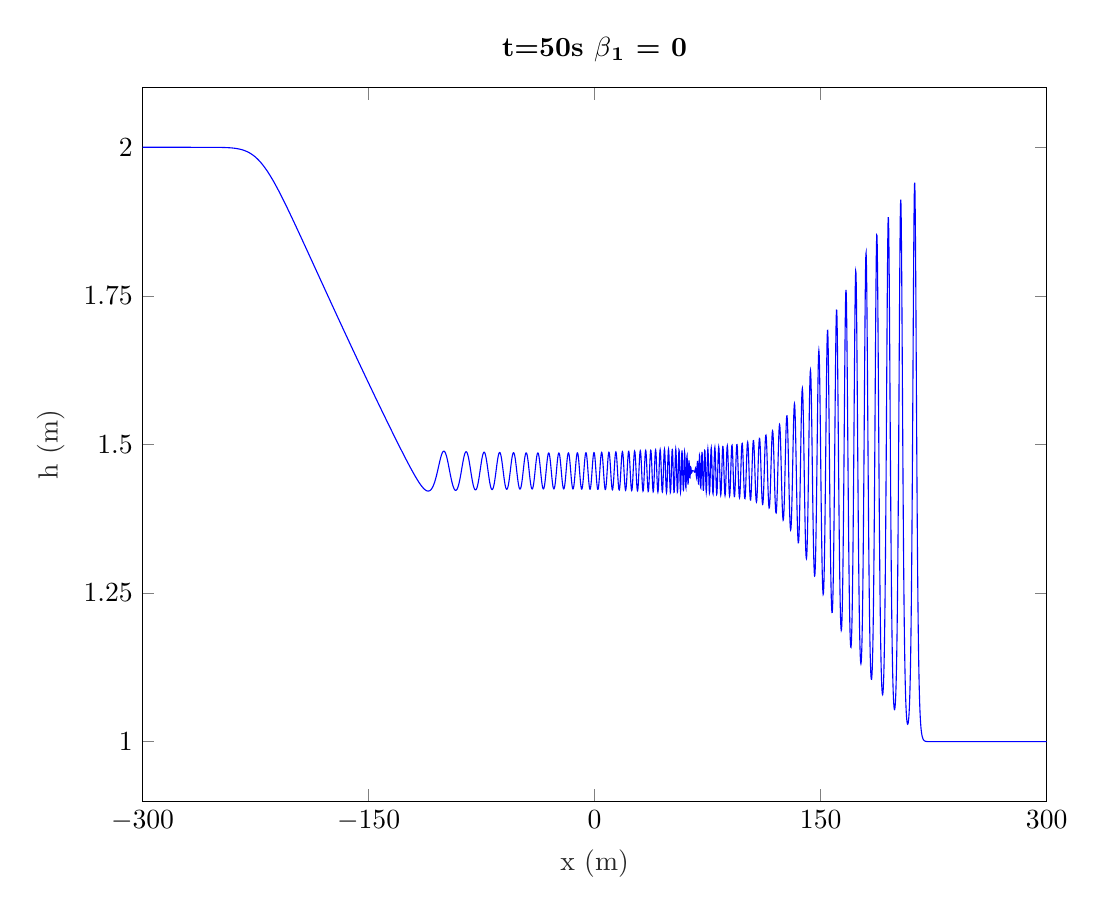
\begin{tikzpicture}

\begin{axis}[%
width=4.521in,
height=3.566in,
at={(0.758in,0.481in)},
scale only axis,
xmin=-300,
xmax=300,
xtick={-300, -150,    0,  150,  300},
xlabel style={font=\color{white!15!black}},
xlabel={x (m)},
ymin=0.9,
ymax=2.1,
ytick={   1, 1.25,  1.5, 1.75,    2},
ylabel style={font=\color{white!15!black}},
ylabel={h (m)},
axis background/.style={fill=white},
title style={font=\bfseries},
title={$\text{t=50s   }\beta{}_\text{1}\text{ = 0}$}
]
\addplot [color=blue, forget plot]
  table[row sep=crcr]{%
-300.18000900045	2\\
-300.030001500075	2\\
-299.8799939997	1.99999999997268\\
-299.729986499325	1.99999999997267\\
-299.57997899895	1.99999999997262\\
-299.429971498575	1.9999999999722\\
-299.2799639982	1.99999999997175\\
-299.129956497825	1.99999999997121\\
-298.97994899745	1.99999999997058\\
-298.829941497075	1.99999999996985\\
-298.6799339967	1.99999999996903\\
-298.529926496325	1.99999999996812\\
-298.37991899595	1.9999999999671\\
-298.229911495575	1.99999999996598\\
-298.0799039952	1.99999999996476\\
-297.929896494825	1.99999999996342\\
-297.77988899445	1.99999999996198\\
-297.629881494075	1.99999999996041\\
-297.4798739937	1.99999999995872\\
-297.329866493325	1.99999999995691\\
-297.17985899295	1.99999999995496\\
-297.029851492575	1.99999999995287\\
-296.8798439922	1.99999999995064\\
-296.729836491825	1.99999999994826\\
-296.57982899145	1.99999999994572\\
-296.429821491075	1.99999999994301\\
-296.2798139907	1.99999999994013\\
-296.129806490325	1.99999999993707\\
-295.979798989949	1.99999999993382\\
-295.829791489574	1.99999999993036\\
-295.679783989199	1.9999999999267\\
-295.529776488824	1.99999999992281\\
-295.379768988449	1.9999999999187\\
-295.229761488074	1.99999999991433\\
-295.079753987699	1.99999999990971\\
-294.929746487324	1.99999999990483\\
-294.779738986949	1.99999999989965\\
-294.629731486574	1.99999999989418\\
-294.479723986199	1.99999999988839\\
-294.329716485824	1.99999999988226\\
-294.179708985449	1.99999999987579\\
-294.029701485074	1.99999999986895\\
-293.879693984699	1.99999999986172\\
-293.729686484324	1.99999999985409\\
-293.579678983949	1.99999999984602\\
-293.429671483574	1.9999999998375\\
-293.279663983199	1.99999999982851\\
-293.129656482824	1.999999999819\\
-292.979648982449	1.99999999980897\\
-292.829641482074	1.99999999979838\\
-292.679633981699	1.99999999978721\\
-292.529626481324	1.99999999977541\\
-292.379618980949	1.99999999976296\\
-292.229611480574	1.99999999974982\\
-292.079603980199	1.99999999973595\\
-291.929596479824	1.99999999972132\\
-291.779588979449	1.99999999970589\\
-291.629581479074	1.99999999968961\\
-291.479573978699	1.99999999967243\\
-291.329566478324	1.99999999965431\\
-291.179558977949	1.99999999963521\\
-291.029551477574	1.99999999961506\\
-290.879543977199	1.9999999995938\\
-290.729536476824	1.99999999957139\\
-290.579528976449	1.99999999954775\\
-290.429521476074	1.99999999952283\\
-290.279513975699	1.99999999949656\\
-290.129506475324	1.99999999946886\\
-289.979498974949	1.99999999943965\\
-289.829491474574	1.99999999940886\\
-289.679483974199	1.99999999937641\\
-289.529476473824	1.9999999993422\\
-289.379468973449	1.99999999930615\\
-289.229461473074	1.99999999926815\\
-289.079453972699	1.9999999992281\\
-288.929446472324	1.99999999918589\\
-288.779438971949	1.99999999914141\\
-288.629431471574	1.99999999909454\\
-288.479423971199	1.99999999904516\\
-288.329416470824	1.99999999899312\\
-288.179408970449	1.9999999989383\\
-288.029401470073	1.99999999888054\\
-287.879393969698	1.9999999988197\\
-287.729386469323	1.9999999987556\\
-287.579378968948	1.99999999868808\\
-287.429371468573	1.99999999861696\\
-287.279363968198	1.99999999854206\\
-287.129356467823	1.99999999846317\\
-286.979348967448	1.99999999838008\\
-286.829341467073	1.99999999829258\\
-286.679333966698	1.99999999820044\\
-286.529326466323	1.99999999810341\\
-286.379318965948	1.99999999800125\\
-286.229311465573	1.99999999789368\\
-286.079303965198	1.99999999778042\\
-285.929296464823	1.99999999766119\\
-285.779288964448	1.99999999753567\\
-285.629281464073	1.99999999740353\\
-285.479273963698	1.99999999726444\\
-285.329266463323	1.99999999711803\\
-285.179258962948	1.99999999696394\\
-285.029251462573	1.99999999680176\\
-284.879243962198	1.99999999663107\\
-284.729236461823	1.99999999645145\\
-284.579228961448	1.99999999626243\\
-284.429221461073	1.99999999606353\\
-284.279213960698	1.99999999585425\\
-284.129206460323	1.99999999563405\\
-283.979198959948	1.99999999540237\\
-283.829191459573	1.99999999515864\\
-283.679183959198	1.99999999490224\\
-283.529176458823	1.99999999463252\\
-283.379168958448	1.9999999943488\\
-283.229161458073	1.99999999405038\\
-283.079153957698	1.9999999937365\\
-282.929146457323	1.99999999340639\\
-282.779138956948	1.99999999305923\\
-282.629131456573	1.99999999269415\\
-282.479123956198	1.99999999231024\\
-282.329116455823	1.99999999190656\\
-282.179108955448	1.99999999148211\\
-282.029101455073	1.99999999103585\\
-281.879093954698	1.99999999056667\\
-281.729086454323	1.99999999007344\\
-281.579078953948	1.99999998955494\\
-281.429071453573	1.9999999890099\\
-281.279063953198	1.999999988437\\
-281.129056452823	1.99999998783485\\
-280.979048952448	1.999999987202\\
-280.829041452073	1.99999998653689\\
-280.679033951698	1.99999998583794\\
-280.529026451323	1.99999998510345\\
-280.379018950948	1.99999998433166\\
-280.229011450573	1.99999998352073\\
-280.079003950197	1.99999998266871\\
-279.928996449822	1.99999998177357\\
-279.778988949447	1.99999998083317\\
-279.628981449072	1.99999997984529\\
-279.478973948697	1.99999997880758\\
-279.328966448322	1.99999997771758\\
-279.178958947947	1.99999997657273\\
-279.028951447572	1.99999997537033\\
-278.878943947197	1.99999997410756\\
-278.728936446822	1.99999997278146\\
-278.578928946447	1.99999997138892\\
-278.428921446072	1.99999996992671\\
-278.278913945697	1.99999996839141\\
-278.128906445322	1.99999996677947\\
-277.978898944947	1.99999996508715\\
-277.828891444572	1.99999996331056\\
-277.678883944197	1.99999996144558\\
-277.528876443822	1.99999995948793\\
-277.378868943447	1.99999995743313\\
-277.228861443072	1.99999995527647\\
-277.078853942697	1.99999995301303\\
-276.928846442322	1.99999995063766\\
-276.778838941947	1.99999994814497\\
-276.628831441572	1.99999994552931\\
-276.478823941197	1.99999994278476\\
-276.328816440822	1.99999993990514\\
-276.178808940447	1.99999993688397\\
-276.028801440072	1.99999993371448\\
-275.878793939697	1.99999993038958\\
-275.728786439322	1.99999992690185\\
-275.578778938947	1.99999992324351\\
-275.428771438572	1.99999991940645\\
-275.278763938197	1.99999991538218\\
-275.128756437822	1.99999991116179\\
-274.978748937447	1.99999990673598\\
-274.828741437072	1.99999990209504\\
-274.678733936697	1.99999989722878\\
-274.528726436322	1.99999989212657\\
-274.378718935947	1.99999988677727\\
-274.228711435572	1.99999988116925\\
-274.078703935197	1.99999987529035\\
-273.928696434822	1.99999986912783\\
-273.778688934447	1.9999998626684\\
-273.628681434072	1.99999985589816\\
-273.478673933697	1.99999984880258\\
-273.328666433322	1.99999984136645\\
-273.178658932947	1.9999998335739\\
-273.028651432572	1.99999982540834\\
-272.878643932197	1.99999981685242\\
-272.728636431822	1.99999980788802\\
-272.578628931447	1.9999997984962\\
-272.428621431072	1.99999978865718\\
-272.278613930697	1.99999977835028\\
-272.128606430321	1.99999976755392\\
-271.978598929946	1.99999975624553\\
-271.828591429571	1.99999974440155\\
-271.678583929196	1.99999973199738\\
-271.528576428821	1.99999971900731\\
-271.378568928446	1.99999970540451\\
-271.228561428071	1.99999969116094\\
-271.078553927696	1.99999967624735\\
-270.928546427321	1.99999966063317\\
-270.778538926946	1.99999964428652\\
-270.628531426571	1.99999962717409\\
-270.478523926196	1.99999960926113\\
-270.328516425821	1.99999959051136\\
-270.178508925446	1.9999995708869\\
-270.028501425071	1.99999955034826\\
-269.878493924696	1.99999952885418\\
-269.728486424321	1.99999950636165\\
-269.578478923946	1.99999948282577\\
-269.428471423571	1.99999945819971\\
-269.278463923196	1.99999943243459\\
-269.128456422821	1.99999940547946\\
-268.978448922446	1.99999937728114\\
-268.828441422071	1.9999993477842\\
-268.678433921696	1.9999993169308\\
-268.528426421321	1.99999928466065\\
-268.378418920946	1.99999925091085\\
-268.228411420571	1.99999921561586\\
-268.078403920196	1.99999917870731\\
-267.928396419821	1.99999914011395\\
-267.778388919446	1.9999990997615\\
-267.628381419071	1.99999905757253\\
-267.478373918696	1.99999901346636\\
-267.328366418321	1.99999896735889\\
-267.178358917946	1.99999891916246\\
-267.028351417571	1.99999886878579\\
-266.878343917196	1.99999881613371\\
-266.728336416821	1.9999987611071\\
-266.578328916446	1.99999870360271\\
-266.428321416071	1.99999864351297\\
-266.278313915696	1.99999858072584\\
-266.128306415321	1.99999851512464\\
-265.978298914946	1.99999844658785\\
-265.828291414571	1.99999837498894\\
-265.678283914196	1.99999830019615\\
-265.528276413821	1.99999822207231\\
-265.378268913446	1.9999981404746\\
-265.228261413071	1.99999805525436\\
-265.078253912696	1.99999796625686\\
-264.928246412321	1.99999787332104\\
-264.778238911946	1.99999777627929\\
-264.628231411571	1.99999767495719\\
-264.478223911196	1.99999756917324\\
-264.328216410821	1.99999745873863\\
-264.178208910446	1.9999973434569\\
-264.02820141007	1.99999722312369\\
-263.878193909695	1.99999709752641\\
-263.72818640932	1.99999696644398\\
-263.578178908945	1.99999682964645\\
-263.42817140857	1.99999668689472\\
-263.278163908195	1.99999653794013\\
-263.12815640782	1.99999638252419\\
-262.978148907445	1.99999622037813\\
-262.82814140707	1.99999605122256\\
-262.678133906695	1.99999587476708\\
-262.52812640632	1.99999569070985\\
-262.378118905945	1.99999549873719\\
-262.22811140557	1.99999529852311\\
-262.078103905195	1.99999508972892\\
-261.92809640482	1.9999948720027\\
-261.778088904445	1.99999464497885\\
-261.62808140407	1.9999944082776\\
-261.478073903695	1.99999416150448\\
-261.32806640332	1.99999390424979\\
-261.178058902945	1.99999363608806\\
-261.02805140257	1.99999335657749\\
-260.878043902195	1.99999306525935\\
-260.72803640182	1.99999276165738\\
-260.578028901445	1.99999244527718\\
-260.42802140107	1.99999211560554\\
-260.278013900695	1.99999177210981\\
-260.12800640032	1.99999141423719\\
-259.977998899945	1.99999104141406\\
-259.82799139957	1.99999065304519\\
-259.677983899195	1.99999024851304\\
-259.52797639882	1.99998982717697\\
-259.377968898445	1.99998938837244\\
-259.22796139807	1.99998893141018\\
-259.077953897695	1.99998845557535\\
-258.92794639732	1.99998796012668\\
-258.777938896945	1.99998744429553\\
-258.62793139657	1.99998690728499\\
-258.477923896195	1.99998634826891\\
-258.32791639582	1.99998576639093\\
-258.177908895445	1.99998516076345\\
-258.02790139507	1.99998453046658\\
-257.877893894695	1.9999838745471\\
-257.72788639432	1.99998319201731\\
-257.577878893945	1.9999824818539\\
-257.42787139357	1.99998174299679\\
-257.277863893195	1.99998097434794\\
-257.12785639282	1.99998017477006\\
-256.977848892445	1.99997934308538\\
-256.82784139207	1.99997847807431\\
-256.677833891695	1.99997757847411\\
-256.52782639132	1.99997664297748\\
-256.377818890945	1.99997567023116\\
-256.22781139057	1.99997465883446\\
-256.077803890195	1.99997360733775\\
-255.927796389819	1.99997251424092\\
-255.777788889444	1.99997137799177\\
-255.627781389069	1.99997019698443\\
-255.477773888694	1.99996896955764\\
-255.327766388319	1.99996769399306\\
-255.177758887944	1.99996636851352\\
-255.027751387569	1.99996499128116\\
-254.877743887194	1.99996356039566\\
-254.727736386819	1.99996207389225\\
-254.577728886444	1.99996052973983\\
-254.427721386069	1.99995892583894\\
-254.277713885694	1.99995726001972\\
-254.127706385319	1.99995553003983\\
-253.977698884944	1.99995373358226\\
-253.827691384569	1.99995186825318\\
-253.677683884194	1.99994993157964\\
-253.527676383819	1.9999479210073\\
-253.377668883444	1.99994583389805\\
-253.227661383069	1.99994366752759\\
-253.077653882694	1.99994141908299\\
-252.927646382319	1.99993908566011\\
-252.777638881944	1.99993666426105\\
-252.627631381569	1.99993415179154\\
-252.477623881194	1.99993154505815\\
-252.327616380819	1.99992884076561\\
-252.177608880444	1.99992603551395\\
-252.027601380069	1.99992312579566\\
-251.877593879694	1.9999201079927\\
-251.727586379319	1.99991697837353\\
-251.577578878944	1.99991373309006\\
-251.427571378569	1.9999103681745\\
-251.277563878194	1.99990687953618\\
-251.127556377819	1.99990326295833\\
-250.977548877444	1.99989951409475\\
-250.827541377069	1.99989562846641\\
-250.677533876694	1.99989160145808\\
-250.527526376319	1.99988742831477\\
-250.377518875944	1.9998831041382\\
-250.227511375569	1.99987862388318\\
-250.077503875194	1.99987398235388\\
-249.927496374819	1.99986917420015\\
-249.777488874444	1.99986419391363\\
-249.627481374069	1.99985903582394\\
-249.477473873694	1.9998536940947\\
-249.327466373319	1.99984816271955\\
-249.177458872944	1.99984243551807\\
-249.027451372569	1.99983650613168\\
-248.877443872194	1.99983036801947\\
-248.727436371819	1.99982401445393\\
-248.577428871444	1.99981743851665\\
-248.427421371069	1.99981063309399\\
-248.277413870694	1.99980359087266\\
-248.127406370319	1.99979630433526\\
-247.977398869943	1.99978876575572\\
-247.827391369568	1.99978096719479\\
-247.677383869193	1.99977290049536\\
-247.527376368818	1.99976455727783\\
-247.377368868443	1.99975592893534\\
-247.227361368068	1.99974700662905\\
-247.077353867693	1.99973778128333\\
-246.927346367318	1.99972824358087\\
-246.777338866943	1.9997183839578\\
-246.627331366568	1.9997081925988\\
-246.477323866193	1.99969765943209\\
-246.327316365818	1.99968677412445\\
-246.177308865443	1.99967552607622\\
-246.027301365068	1.99966390441622\\
-245.877293864693	1.99965189799669\\
-245.727286364318	1.99963949538818\\
-245.577278863943	1.9996266848745\\
-245.427271363568	1.99961345444752\\
-245.277263863193	1.99959979180209\\
-245.127256362818	1.99958568433091\\
-244.977248862443	1.99957111911935\\
-244.827241362068	1.99955608294037\\
-244.677233861693	1.99954056224936\\
-244.527226361318	1.99952454317905\\
-244.377218860943	1.9995080115344\\
-244.227211360568	1.99949095278755\\
-244.077203860193	1.99947335207274\\
-243.927196359818	1.99945519418133\\
-243.777188859443	1.99943646355683\\
-243.627181359068	1.99941714428994\\
-243.477173858693	1.9993972201137\\
-243.327166358318	1.99937667439864\\
-243.177158857943	1.99935549014804\\
-243.027151357568	1.99933364999323\\
-242.877143857193	1.99931113618898\\
-242.727136356818	1.99928793060895\\
-242.577128856443	1.99926401474123\\
-242.427121356068	1.99923936968404\\
-242.277113855693	1.99921397614142\\
-242.127106355318	1.99918781441913\\
-241.977098854943	1.99916086442062\\
-241.827091354568	1.99913310564314\\
-241.677083854193	1.99910451717397\\
-241.527076353818	1.9990750776868\\
-241.377068853443	1.99904476543829\\
-241.227061353068	1.99901355826472\\
-241.077053852693	1.99898143357886\\
-240.927046352318	1.99894836836703\\
-240.777038851943	1.99891433918627\\
-240.627031351568	1.99887932216178\\
-240.477023851193	1.99884329298452\\
-240.327016350818	1.99880622690903\\
-240.177008850443	1.99876809875146\\
-240.027001350068	1.99872888288787\\
-239.876993849692	1.99868855325271\\
-239.726986349317	1.99864708333758\\
-239.576978848942	1.99860444619024\\
-239.426971348567	1.99856061441388\\
-239.276963848192	1.9985155601667\\
-239.126956347817	1.99846925516171\\
-238.976948847442	1.99842167066686\\
-238.826941347067	1.99837277750551\\
-238.676933846692	1.99832254605714\\
-238.526926346317	1.9982709462584\\
-238.376918845942	1.99821794760455\\
-238.226911345567	1.99816351915115\\
-238.076903845192	1.99810762951616\\
-237.926896344817	1.99805024688238\\
-237.776888844442	1.99799133900023\\
-237.626881344067	1.99793087319096\\
-237.476873843692	1.99786881635016\\
-237.326866343317	1.99780513495173\\
-237.176858842942	1.99773979505224\\
-237.026851342567	1.99767276229563\\
-236.876843842192	1.99760400191839\\
-236.726836341817	1.99753347875515\\
-236.576828841442	1.99746115724464\\
-236.426821341067	1.99738700143616\\
-236.276813840692	1.99731097499644\\
-236.126806340317	1.99723304121692\\
-235.976798839942	1.99715316302152\\
-235.826791339567	1.99707130297487\\
-235.676783839192	1.99698742329096\\
-235.526776338817	1.99690148584226\\
-235.376768838442	1.99681345216931\\
-235.226761338067	1.99672328349077\\
-235.076753837692	1.99663094071396\\
-234.926746337317	1.99653638444584\\
-234.776738836942	1.99643957500445\\
-234.626731336567	1.99634047243089\\
-234.476723836192	1.99623903650169\\
-234.326716335817	1.9961352267417\\
-234.176708835442	1.99602900243744\\
-234.026701335067	1.9959203226509\\
-233.876693834692	1.99580914623383\\
-233.726686334317	1.99569543184246\\
-233.576678833942	1.99557913795273\\
-233.426671333567	1.99546022287591\\
-233.276663833192	1.9953386447747\\
-233.126656332817	1.99521436167978\\
-232.976648832442	1.99508733150676\\
-232.826641332067	1.99495751207361\\
-232.676633831692	1.99482486111842\\
-232.526626331317	1.99468933631768\\
-232.376618830942	1.99455089530487\\
-232.226611330567	1.99440949568946\\
-232.076603830192	1.99426509507632\\
-231.926596329817	1.99411765108545\\
-231.776588829441	1.99396712137207\\
-231.626581329066	1.99381346364707\\
-231.476573828691	1.99365663569775\\
-231.326566328316	1.9934965954089\\
-231.176558827941	1.99333330078413\\
-231.026551327566	1.99316670996751\\
-230.876543827191	1.99299678126544\\
-230.726536326816	1.99282347316876\\
-230.576528826441	1.9926467443751\\
-230.426521326066	1.99246655381142\\
-230.276513825691	1.99228286065668\\
-230.126506325316	1.99209562436474\\
-229.976498824941	1.99190480468737\\
-229.826491324566	1.99171036169732\\
-229.676483824191	1.99151225581157\\
-229.526476323816	1.99131044781459\\
-229.376468823441	1.99110489888162\\
-229.226461323066	1.99089557060206\\
-229.076453822691	1.99068242500275\\
-228.926446322316	1.99046542457128\\
-228.776438821941	1.99024453227924\\
-228.626431321566	1.99001971160536\\
-228.476423821191	1.98979092655857\\
-228.326416320816	1.9895581417009\\
-228.176408820441	1.98932132217024\\
-228.026401320066	1.98908043370291\\
-227.876393819691	1.98883544265597\\
-227.726386319316	1.9885863160294\\
-227.576378818941	1.98833302148788\\
-227.426371318566	1.98807552738236\\
-227.276363818191	1.98781380277126\\
-227.126356317816	1.98754781744138\\
-226.976348817441	1.98727754192838\\
-226.826341317066	1.98700294753689\\
-226.676333816691	1.98672400636018\\
-226.526326316316	1.98644069129937\\
-226.376318815941	1.98615297608222\\
-226.226311315566	1.98586083528133\\
-226.076303815191	1.9855642443319\\
-225.926296314816	1.98526317954886\\
-225.776288814441	1.98495761814352\\
-225.626281314066	1.98464753823955\\
-225.476273813691	1.98433291888837\\
-225.326266313316	1.98401374008391\\
-225.176258812941	1.98368998277674\\
-225.026251312566	1.98336162888744\\
-224.876243812191	1.98302866131939\\
-224.726236311816	1.98269106397073\\
-224.576228811441	1.98234882174569\\
-224.426221311066	1.98200192056514\\
-224.276213810691	1.98165034737634\\
-224.126206310316	1.98129409016201\\
-223.976198809941	1.98093313794852\\
-223.826191309565	1.98056748081334\\
-223.67618380919	1.98019710989169\\
-223.526176308815	1.97982201738232\\
-223.37616880844	1.97944219655252\\
-223.226161308065	1.9790576417423\\
-223.07615380769	1.97866834836769\\
-222.926146307315	1.97827431292324\\
-222.77613880694	1.97787553298367\\
-222.626131306565	1.97747200720464\\
-222.47612380619	1.97706373532277\\
-222.326116305815	1.97665071815466\\
-222.17610880544	1.97623295759523\\
-222.026101305065	1.97581045661512\\
-221.87609380469	1.97538321925727\\
-221.726086304315	1.9749512506327\\
-221.57607880394	1.97451455691543\\
-221.426071303565	1.97407314533663\\
-221.27606380319	1.9736270241779\\
-221.126056302815	1.9731762027638\\
-220.97604880244	1.9727206914536\\
-220.826041302065	1.97226050163221\\
-220.67603380169	1.97179564570043\\
-220.526026301315	1.97132613706435\\
-220.37601880094	1.97085199012411\\
-220.226011300565	1.97037322026191\\
-220.07600380019	1.96988984382934\\
-219.925996299815	1.969401878134\\
-219.77598879944	1.9689093414255\\
-219.625981299065	1.96841225288082\\
-219.47597379869	1.96791063258902\\
-219.325966298315	1.96740450153539\\
-219.17595879794	1.966893881585\\
-219.025951297565	1.96637879546574\\
-218.87594379719	1.96585926675078\\
-218.725936296815	1.96533531984059\\
-218.57592879644	1.96480697994438\\
-218.425921296065	1.96427427306124\\
-218.27591379569	1.9637372259607\\
-218.125906295315	1.96319586616298\\
-217.97589879494	1.96265022191887\\
-217.825891294565	1.96210032218915\\
-217.67588379419	1.96154619662384\\
-217.525876293815	1.96098787554104\\
-217.37586879344	1.96042538990553\\
-217.225861293065	1.95985877130719\\
-217.07585379269	1.95928805193908\\
-216.925846292315	1.95871326457544\\
-216.77583879194	1.95813444254946\\
-216.625831291565	1.95755161973095\\
-216.47582379119	1.95696483050389\\
-216.325816290815	1.95637410974386\\
-216.17580879044	1.95577949279548\\
-216.025801290065	1.95518101544975\\
-215.875793789689	1.95457871392138\\
-215.725786289314	1.95397262482624\\
-215.575778788939	1.95336278515866\\
-215.425771288564	1.95274923226901\\
-215.275763788189	1.95213200384118\\
-215.125756287814	1.95151113787027\\
-214.975748787439	1.9508866726404\\
-214.825741287064	1.95025864670262\\
-214.675733786689	1.9496270988531\\
-214.525726286314	1.94899206811134\\
-214.375718785939	1.94835359369879\\
-214.225711285564	1.94771171501756\\
-214.075703785189	1.94706647162941\\
-213.925696284814	1.94641790323504\\
-213.775688784439	1.94576604965366\\
-213.625681284064	1.94511095080279\\
-213.475673783689	1.94445264667848\\
-213.325666283314	1.94379117733575\\
-213.175658782939	1.94312658286947\\
-213.025651282564	1.94245890339553\\
-212.875643782189	1.94178817903236\\
-212.725636281814	1.94111444988292\\
-212.575628781439	1.94043775601696\\
-212.425621281064	1.93975813745381\\
-212.275613780689	1.9390756341454\\
-212.125606280314	1.9383902859599\\
-211.975598779939	1.93770213266559\\
-211.825591279564	1.93701121391534\\
-211.675583779189	1.93631756923131\\
-211.525576278814	1.93562123799032\\
-211.375568778439	1.93492225940949\\
-211.225561278064	1.9342206725324\\
-211.075553777689	1.9335165162157\\
-210.925546277314	1.93280982911614\\
-210.775538776939	1.9321006496781\\
-210.625531276564	1.93138901612151\\
-210.475523776189	1.93067496643031\\
-210.325516275814	1.92995853834128\\
-210.175508775439	1.92923976933336\\
-210.025501275064	1.92851869661744\\
-209.875493774689	1.92779535712658\\
-209.725486274314	1.92706978750667\\
-209.575478773939	1.92634202410756\\
-209.425471273564	1.92561210297456\\
-209.275463773189	1.92488005984052\\
-209.125456272814	1.92414593011815\\
-208.975448772439	1.92340974889296\\
-208.825441272064	1.92267155091647\\
-208.675433771689	1.9219313705999\\
-208.525426271314	1.9211892420083\\
-208.375418770939	1.92044519885503\\
-208.225411270564	1.91969927449662\\
-208.075403770189	1.91895150192813\\
-207.925396269813	1.91820191377873\\
-207.775388769438	1.91745054230781\\
-207.625381269063	1.91669741940137\\
-207.475373768688	1.91594257656873\\
-207.325366268313	1.91518604493975\\
-207.175358767938	1.91442785526219\\
-207.025351267563	1.91366803789957\\
-206.875343767188	1.91290662282926\\
-206.725336266813	1.91214363964091\\
-206.575328766438	1.91137911753519\\
-206.425321266063	1.91061308532286\\
-206.275313765688	1.90984557142406\\
-206.125306265313	1.90907660386795\\
-205.975298764938	1.90830621029255\\
-205.825291264563	1.90753441794496\\
-205.675283764188	1.90676125368165\\
-205.525276263813	1.9059867439692\\
-205.375268763438	1.90521091488511\\
-205.225261263063	1.90443379211895\\
-205.075253762688	1.90365540097363\\
-204.925246262313	1.90287576636697\\
-204.775238761938	1.9020949128334\\
-204.625231261563	1.9013128645259\\
-204.475223761188	1.9005296452181\\
-204.325216260813	1.89974527830652\\
-204.175208760438	1.89895978681304\\
-204.025201260063	1.89817319338751\\
-203.875193759688	1.89738552031047\\
-203.725186259313	1.89659678949604\\
-203.575178758938	1.89580702249496\\
-203.425171258563	1.89501624049773\\
-203.275163758188	1.89422446433785\\
-203.125156257813	1.89343171449524\\
-202.975148757438	1.89263801109967\\
-202.825141257063	1.8918433739344\\
-202.675133756688	1.89104782243976\\
-202.525126256313	1.89025137571699\\
-202.375118755938	1.88945405253198\\
-202.225111255563	1.88865587131924\\
-202.075103755188	1.8878568501858\\
-201.925096254813	1.88705700691526\\
-201.775088754438	1.88625635897185\\
-201.625081254063	1.88545492350456\\
-201.475073753688	1.88465271735125\\
-201.325066253313	1.88384975704291\\
-201.175058752938	1.88304605880782\\
-201.025051252563	1.88224163857583\\
-200.875043752188	1.88143651198265\\
-200.725036251813	1.8806306943741\\
-200.575028751438	1.87982420081043\\
-200.425021251063	1.87901704607059\\
-200.275013750688	1.87820924465661\\
-200.125006250313	1.87740081079787\\
-199.974998749937	1.8765917584554\\
-199.824991249562	1.87578210132618\\
-199.674983749187	1.87497185284748\\
-199.524976248812	1.87416102620108\\
-199.374968748437	1.87334963431754\\
-199.224961248062	1.87253768988049\\
-199.074953747687	1.87172520533078\\
-198.924946247312	1.87091219287072\\
-198.774938746937	1.87009866446823\\
-198.624931246562	1.86928463186101\\
-198.474923746187	1.8684701065606\\
-198.324916245812	1.86765509985645\\
-198.174908745437	1.86683962282003\\
-198.024901245062	1.86602368630875\\
-197.874893744687	1.86520730096995\\
-197.724886244312	1.86439047724483\\
-197.574878743937	1.86357322537233\\
-197.424871243562	1.86275555539294\\
-197.274863743187	1.86193747715252\\
-197.124856242812	1.86111900030602\\
-196.974848742437	1.86030013432122\\
-196.824841242062	1.85948088848231\\
-196.674833741687	1.85866127189358\\
-196.524826241312	1.8578412934829\\
-196.374818740937	1.85702096200529\\
-196.224811240562	1.8562002860463\\
-196.074803740187	1.85537927402548\\
-195.924796239812	1.85455793419972\\
-195.774788739437	1.85373627466652\\
-195.624781239062	1.85291430336726\\
-195.474773738687	1.8520920280904\\
-195.324766238312	1.85126945647465\\
-195.174758737937	1.85044659601201\\
-195.024751237562	1.84962345405086\\
-194.874743737187	1.84880003779892\\
-194.724736236812	1.84797635432621\\
-194.574728736437	1.84715241056794\\
-194.424721236062	1.84632821332731\\
-194.274713735687	1.84550376927835\\
-194.124706235312	1.8446790849686\\
-193.974698734937	1.84385416682183\\
-193.824691234562	1.84302902114063\\
-193.674683734187	1.84220365410907\\
-193.524676233812	1.84137807179512\\
-193.374668733437	1.84055228015326\\
-193.224661233062	1.8397262850268\\
-193.074653732687	1.83890009215035\\
-192.924646232312	1.83807370715211\\
-192.774638731937	1.83724713555618\\
-192.624631231562	1.83642038278482\\
-192.474623731187	1.83559345416061\\
-192.324616230812	1.83476635490865\\
-192.174608730437	1.83393909015863\\
-192.024601230062	1.83311166494692\\
-191.874593729686	1.83228408421857\\
-191.724586229311	1.83145635282933\\
-191.574578728936	1.83062847554752\\
-191.424571228561	1.829800457056\\
-191.274563728186	1.82897230195395\\
-191.124556227811	1.82814401475874\\
-190.974548727436	1.82731559990766\\
-190.824541227061	1.82648706175971\\
-190.674533726686	1.82565840459724\\
-190.524526226311	1.82482963262762\\
-190.374518725936	1.8240007499849\\
-190.224511225561	1.82317176073134\\
-190.074503725186	1.82234266885901\\
-189.924496224811	1.82151347829126\\
-189.774488724436	1.82068419288423\\
-189.624481224061	1.81985481642831\\
-189.474473723686	1.81902535264949\\
-189.324466223311	1.81819580521082\\
-189.174458722936	1.81736617771371\\
-189.024451222561	1.81653647369925\\
-188.874443722186	1.81570669664953\\
-188.724436221811	1.81487684998888\\
-188.574428721436	1.81404693708508\\
-188.424421221061	1.81321696125059\\
-188.274413720686	1.81238692574373\\
-188.124406220311	1.81155683376978\\
-187.974398719936	1.81072668848214\\
-187.824391219561	1.80989649298342\\
-187.674383719186	1.8090662503265\\
-187.524376218811	1.80823596351556\\
-187.374368718436	1.80740563550712\\
-187.224361218061	1.80657526921101\\
-187.074353717686	1.80574486749137\\
-186.924346217311	1.8049144331676\\
-186.774338716936	1.80408396901525\\
-186.624331216561	1.80325347776693\\
-186.474323716186	1.80242296211326\\
-186.324316215811	1.80159242470364\\
-186.174308715436	1.80076186814716\\
-186.024301215061	1.79993129501337\\
-185.874293714686	1.79910070783314\\
-185.724286214311	1.79827010909941\\
-185.574278713936	1.79743950126796\\
-185.424271213561	1.79660888675817\\
-185.274263713186	1.79577826795372\\
-185.124256212811	1.79494764720337\\
-184.974248712436	1.79411702682158\\
-184.824241212061	1.79328640908924\\
-184.674233711686	1.79245579625433\\
-184.524226211311	1.79162519053256\\
-184.374218710936	1.790794594108\\
-184.224211210561	1.78996400913374\\
-184.074203710186	1.78913343773243\\
-183.92419620981	1.78830288199693\\
-183.774188709435	1.78747234399087\\
-183.62418120906	1.78664182574921\\
-183.474173708685	1.7858113292788\\
-183.32416620831	1.78498085655891\\
-183.174158707935	1.78415040954178\\
-183.02415120756	1.78331999015311\\
-182.874143707185	1.7824896002926\\
-182.72413620681	1.78165924183439\\
-182.574128706435	1.78082891662759\\
-182.42412120606	1.77999862649673\\
-182.274113705685	1.77916837324224\\
-182.12410620531	1.77833815864086\\
-181.974098704935	1.77750798444613\\
-181.82409120456	1.77667785238878\\
-181.674083704185	1.77584776417719\\
-181.52407620381	1.77501772149777\\
-181.374068703435	1.77418772601537\\
-181.22406120306	1.7733577793737\\
-181.074053702685	1.77252788319567\\
-180.92404620231	1.77169803908381\\
-180.774038701935	1.77086824862063\\
-180.62403120156	1.77003851336896\\
-180.474023701185	1.76920883487233\\
-180.32401620081	1.76837921465531\\
-180.174008700435	1.76754965422384\\
-180.02400120006	1.76672015506555\\
-179.873993699685	1.76589071865014\\
-179.72398619931	1.76506134642963\\
-179.573978698935	1.76423203983872\\
-179.42397119856	1.76340280029508\\
-179.273963698185	1.76257362919963\\
-179.12395619781	1.76174452793686\\
-178.973948697435	1.76091549787512\\
-178.82394119706	1.76008654036687\\
-178.673933696685	1.75925765674898\\
-178.52392619631	1.75842884834301\\
-178.373918695935	1.75760011645544\\
-178.22391119556	1.75677146237795\\
-178.073903695185	1.75594288738769\\
-177.92389619481	1.75511439274749\\
-177.773888694435	1.75428597970614\\
-177.62388119406	1.7534576494986\\
-177.473873693685	1.75262940334628\\
-177.32386619331	1.75180124245722\\
-177.173858692935	1.75097316802633\\
-177.02385119256	1.75014518123565\\
-176.873843692185	1.74931728325452\\
-176.72383619181	1.74848947523979\\
-176.573828691435	1.74766175833609\\
-176.42382119106	1.74683413367597\\
-176.273813690685	1.74600660238014\\
-176.123806190309	1.74517916555764\\
-175.973798689934	1.74435182430606\\
-175.823791189559	1.74352457971174\\
-175.673783689184	1.74269743284991\\
-175.523776188809	1.74187038478491\\
-175.373768688434	1.74104343657039\\
-175.223761188059	1.74021658924942\\
-175.073753687684	1.73938984385475\\
-174.923746187309	1.7385632014089\\
-174.773738686934	1.7377366629244\\
-174.623731186559	1.7369102294039\\
-174.473723686184	1.73608390184038\\
-174.323716185809	1.73525768121725\\
-174.173708685434	1.73443156850858\\
-174.023701185059	1.73360556467919\\
-173.873693684684	1.73277967068487\\
-173.723686184309	1.73195388747244\\
-173.573678683934	1.73112821597999\\
-173.423671183559	1.73030265713696\\
-173.273663683184	1.72947721186431\\
-173.123656182809	1.72865188107466\\
-172.973648682434	1.72782666567243\\
-172.823641182059	1.72700156655397\\
-172.673633681684	1.72617658460767\\
-172.523626181309	1.72535172071415\\
-172.373618680934	1.72452697574634\\
-172.223611180559	1.72370235056961\\
-172.073603680184	1.72287784604195\\
-171.923596179809	1.722053463014\\
-171.773588679434	1.72122920232927\\
-171.623581179059	1.7204050648242\\
-171.473573678684	1.7195810513283\\
-171.323566178309	1.71875716266426\\
-171.173558677934	1.71793339964806\\
-171.023551177559	1.7171097630891\\
-170.873543677184	1.71628625379031\\
-170.723536176809	1.71546287254824\\
-170.573528676434	1.71463962015319\\
-170.423521176059	1.71381649738932\\
-170.273513675684	1.71299350503474\\
-170.123506175309	1.71217064386161\\
-169.973498674934	1.71134791463628\\
-169.823491174559	1.71052531811936\\
-169.673483674184	1.70970285506582\\
-169.523476173809	1.70888052622511\\
-169.373468673434	1.70805833234124\\
-169.223461173059	1.70723627415288\\
-169.073453672684	1.70641435239349\\
-168.923446172309	1.70559256779134\\
-168.773438671934	1.7047709210697\\
-168.623431171559	1.70394941294683\\
-168.473423671184	1.70312804413617\\
-168.323416170809	1.70230681534636\\
-168.173408670434	1.70148572728136\\
-168.023401170058	1.70066478064054\\
-167.873393669683	1.69984397611875\\
-167.723386169308	1.69902331440642\\
-167.573378668933	1.69820279618966\\
-167.423371168558	1.69738242215032\\
-167.273363668183	1.69656219296607\\
-167.123356167808	1.69574210931053\\
-166.973348667433	1.6949221718533\\
-166.823341167058	1.69410238126006\\
-166.673333666683	1.69328273819266\\
-166.523326166308	1.69246324330919\\
-166.373318665933	1.69164389726408\\
-166.223311165558	1.69082470070816\\
-166.073303665183	1.69000565428873\\
-165.923296164808	1.68918675864966\\
-165.773288664433	1.68836801443145\\
-165.623281164058	1.68754942227134\\
-165.473273663683	1.68673098280335\\
-165.323266163308	1.68591269665834\\
-165.173258662933	1.68509456446415\\
-165.023251162558	1.68427658684564\\
-164.873243662183	1.68345876442473\\
-164.723236161808	1.68264109782053\\
-164.573228661433	1.68182358764938\\
-164.423221161058	1.68100623452496\\
-164.273213660683	1.68018903905829\\
-164.123206160308	1.67937200185789\\
-163.973198659933	1.67855512352979\\
-163.823191159558	1.67773840467763\\
-163.673183659183	1.67692184590272\\
-163.523176158808	1.67610544780412\\
-163.373168658433	1.67528921097871\\
-163.223161158058	1.67447313602124\\
-163.073153657683	1.67365722352443\\
-162.923146157308	1.67284147407903\\
-162.773138656933	1.67202588827388\\
-162.623131156558	1.67121046669601\\
-162.473123656183	1.67039520993066\\
-162.323116155808	1.66958011856139\\
-162.173108655433	1.66876519317013\\
-162.023101155058	1.66795043433729\\
-161.873093654683	1.66713584264174\\
-161.723086154308	1.66632141866099\\
-161.573078653933	1.66550716297118\\
-161.423071153558	1.66469307614718\\
-161.273063653183	1.66387915876264\\
-161.123056152808	1.66306541139012\\
-160.973048652433	1.66225183460105\\
-160.823041152058	1.66143842896592\\
-160.673033651683	1.66062519505426\\
-160.523026151308	1.65981213343476\\
-160.373018650933	1.65899924467532\\
-160.223011150558	1.65818652934313\\
-160.073003650182	1.65737398800471\\
-159.922996149807	1.65656162122604\\
-159.772988649432	1.65574942957258\\
-159.622981149057	1.65493741360936\\
-159.472973648682	1.65412557390105\\
-159.322966148307	1.65331391101202\\
-159.172958647932	1.65250242550645\\
-159.022951147557	1.65169111794835\\
-158.872943647182	1.65087998890167\\
-158.722936146807	1.65006903893037\\
-158.572928646432	1.64925826859848\\
-158.422921146057	1.64844767847017\\
-158.272913645682	1.64763726910985\\
-158.122906145307	1.64682704108222\\
-157.972898644932	1.64601699495236\\
-157.822891144557	1.64520713128581\\
-157.672883644182	1.64439745064864\\
-157.522876143807	1.6435879536075\\
-157.372868643432	1.64277864072977\\
-157.222861143057	1.64196951258354\\
-157.072853642682	1.64116056973779\\
-156.922846142307	1.6403518127624\\
-156.772838641932	1.63954324222826\\
-156.622831141557	1.63873485870734\\
-156.472823641182	1.63792666277279\\
-156.322816140807	1.63711865499901\\
-156.172808640432	1.63631083596172\\
-156.022801140057	1.63550320623808\\
-155.872793639682	1.63469576640676\\
-155.722786139307	1.633888517048\\
-155.572778638932	1.63308145874374\\
-155.422771138557	1.6322745920777\\
-155.272763638182	1.63146791763545\\
-155.122756137807	1.63066143600452\\
-154.972748637432	1.62985514777447\\
-154.822741137057	1.62904905353702\\
-154.672733636682	1.62824315388611\\
-154.522726136307	1.62743744941803\\
-154.372718635932	1.62663194073147\\
-154.222711135557	1.62582662842767\\
-154.072703635182	1.62502151311048\\
-153.922696134807	1.62421659538651\\
-153.772688634432	1.62341187586517\\
-153.622681134057	1.62260735515882\\
-153.472673633682	1.62180303388286\\
-153.322666133307	1.62099891265585\\
-153.172658632932	1.62019499209959\\
-153.022651132557	1.61939127283929\\
-152.872643632182	1.61858775550361\\
-152.722636131807	1.61778444072483\\
-152.572628631432	1.61698132913894\\
-152.422621131057	1.61617842138576\\
-152.272613630682	1.6153757181091\\
-152.122606130307	1.61457321995681\\
-151.972598629931	1.61377092758096\\
-151.822591129556	1.61296884163797\\
-151.672583629181	1.6121669627887\\
-151.522576128806	1.61136529169862\\
-151.372568628431	1.61056382903791\\
-151.222561128056	1.60976257548163\\
-151.072553627681	1.60896153170986\\
-150.922546127306	1.60816069840779\\
-150.772538626931	1.60736007626593\\
-150.622531126556	1.60655966598022\\
-150.472523626181	1.6057594682522\\
-150.322516125806	1.60495948378912\\
-150.172508625431	1.60415971330416\\
-150.022501125056	1.60336015751656\\
-149.872493624681	1.60256081715176\\
-149.722486124306	1.6017616929416\\
-149.572478623931	1.60096278562447\\
-149.422471123556	1.60016409594549\\
-149.272463623181	1.59936562465668\\
-149.122456122806	1.59856737251716\\
-148.972448622431	1.59776934029331\\
-148.822441122056	1.59697152875896\\
-148.672433621681	1.5961739386956\\
-148.522426121306	1.59537657089255\\
-148.372418620931	1.59457942614719\\
-148.222411120556	1.59378250526514\\
-148.072403620181	1.59298580906048\\
-147.922396119806	1.59218933835597\\
-147.772388619431	1.59139309398324\\
-147.622381119056	1.59059707678305\\
-147.472373618681	1.58980128760552\\
-147.322366118306	1.5890057273103\\
-147.172358617931	1.58821039676691\\
-147.022351117556	1.58741529685489\\
-146.872343617181	1.58662042846411\\
-146.722336116806	1.58582579249502\\
-146.572328616431	1.58503138985888\\
-146.422321116056	1.58423722147805\\
-146.272313615681	1.58344328828629\\
-146.122306115306	1.58264959122898\\
-145.972298614931	1.58185613126349\\
-145.822291114556	1.58106290935939\\
-145.672283614181	1.58026992649882\\
-145.522276113806	1.57947718367678\\
-145.372268613431	1.57868468190141\\
-145.222261113056	1.5778924221944\\
-145.072253612681	1.57710040559124\\
-144.922246112306	1.57630863314161\\
-144.772238611931	1.57551710590972\\
-144.622231111556	1.57472582497466\\
-144.472223611181	1.5739347914308\\
-144.322216110806	1.57314400638813\\
-144.172208610431	1.57235347097269\\
-144.022201110056	1.57156318632693\\
-143.87219360968	1.57077315361015\\
-143.722186109305	1.56998337399891\\
-143.57217860893	1.56919384868746\\
-143.422171108555	1.56840457888818\\
-143.27216360818	1.56761556583206\\
-143.122156107805	1.56682681076912\\
-142.97214860743	1.56603831496894\\
-142.822141107055	1.56525007972114\\
-142.67213360668	1.56446210633586\\
-142.522126106305	1.56367439614432\\
-142.37211860593	1.56288695049931\\
-142.222111105555	1.56209977077579\\
-142.07210360518	1.56131285837143\\
-141.922096104805	1.56052621470719\\
-141.77208860443	1.55973984122791\\
-141.622081104055	1.55895373940294\\
-141.47207360368	1.55816791072678\\
-141.322066103305	1.55738235671971\\
-141.17205860293	1.55659707892847\\
-141.022051102555	1.55581207892694\\
-140.87204360218	1.55502735831685\\
-140.722036101805	1.55424291872852\\
-140.57202860143	1.55345876182158\\
-140.422021101055	1.5526748892858\\
-140.27201360068	1.5518913028418\\
-140.122006100305	1.55110800424197\\
-139.97199859993	1.55032499527121\\
-139.821991099555	1.54954227774787\\
-139.67198359918	1.54875985352461\\
-139.521976098805	1.54797772448934\\
-139.37196859843	1.54719589256615\\
-139.221961098055	1.54641435971629\\
-139.07195359768	1.5456331279392\\
-138.921946097305	1.54485219927352\\
-138.77193859693	1.54407157579817\\
-138.621931096555	1.54329125963347\\
-138.47192359618	1.54251125294223\\
-138.321916095805	1.54173155793099\\
-138.17190859543	1.54095217685118\\
-138.021901095055	1.54017311200037\\
-137.87189359468	1.53939436572361\\
-137.721886094305	1.53861594041468\\
-137.57187859393	1.53783783851751\\
-137.421871093555	1.53706006252759\\
-137.27186359318	1.53628261499344\\
-137.121856092805	1.53550549851807\\
-136.97184859243	1.5347287157606\\
-136.821841092055	1.53395226943781\\
-136.67183359168	1.53317616232585\\
-136.521826091305	1.53240039726192\\
-136.37181859093	1.53162497714605\\
-136.221811090555	1.53084990494292\\
-136.07180359018	1.5300751836838\\
-135.921796089805	1.52930081646842\\
-135.771788589429	1.52852680646707\\
-135.621781089054	1.52775315692263\\
-135.471773588679	1.52697987115276\\
-135.321766088304	1.52620695255212\\
-135.171758587929	1.52543440459468\\
-135.021751087554	1.52466223083612\\
-134.871743587179	1.52389043491626\\
-134.721736086804	1.52311902056166\\
-134.571728586429	1.52234799158823\\
-134.421721086054	1.52157735190398\\
-134.271713585679	1.52080710551186\\
-134.121706085304	1.52003725651265\\
-133.971698584929	1.51926780910806\\
-133.821691084554	1.5184987676038\\
-133.671683584179	1.51773013641286\\
-133.521676083804	1.51696192005891\\
-133.371668583429	1.51619412317974\\
-133.221661083054	1.51542675053089\\
-133.071653582679	1.51465980698943\\
-132.921646082304	1.51389329755778\\
-132.771638581929	1.51312722736777\\
-132.621631081554	1.51236160168481\\
-132.471623581179	1.5115964259122\\
-132.321616080804	1.51083170559562\\
-132.171608580429	1.51006744642776\\
-132.021601080054	1.50930365425316\\
-131.871593579679	1.50854033507319\\
-131.721586079304	1.50777749505127\\
-131.571578578929	1.50701514051819\\
-131.421571078554	1.50625327797776\\
-131.271563578179	1.50549191411256\\
-131.121556077804	1.50473105578998\\
-130.971548577429	1.50397071006844\\
-130.821541077054	1.50321088420389\\
-130.671533576679	1.50245158565655\\
-130.521526076304	1.50169282209786\\
-130.371518575929	1.50093460141781\\
-130.221511075554	1.5001769317324\\
-130.071503575179	1.49941982139157\\
-129.921496074804	1.49866327898726\\
-129.771488574429	1.49790731336192\\
-129.621481074054	1.49715193361731\\
-129.471473573679	1.49639714912363\\
-129.321466073304	1.49564296952902\\
-129.171458572929	1.49488940476947\\
-129.021451072554	1.49413646507909\\
-128.871443572179	1.49338416100081\\
-128.721436071804	1.4926325033975\\
-128.571428571429	1.49188150346353\\
-128.421421071054	1.49113117273684\\
-128.271413570679	1.49038152311146\\
-128.121406070304	1.48963256685054\\
-127.971398569929	1.48888431659996\\
-127.821391069553	1.48813678540241\\
-127.671383569178	1.48738998671217\\
-127.521376068803	1.48664393441038\\
-127.371368568428	1.48589864282105\\
-127.221361068053	1.48515412672761\\
-127.071353567678	1.48441040139032\\
-126.921346067303	1.48366748256424\\
-126.771338566928	1.48292538651804\\
-126.621331066553	1.48218413005361\\
-126.471323566178	1.48144373052645\\
-126.321316065803	1.48070420586698\\
-126.171308565428	1.4799655746027\\
-126.021301065053	1.4792278558813\\
-125.871293564678	1.47849106949484\\
-125.721286064303	1.4777552359048\\
-125.571278563928	1.47702037626841\\
-125.421271063553	1.47628651246591\\
-125.271263563178	1.47555366712915\\
-125.121256062803	1.47482186367135\\
-124.971248562428	1.47409112631812\\
-124.821241062053	1.4733614801399\\
-124.671233561678	1.47263295108578\\
-124.521226061303	1.47190556601882\\
-124.371218560928	1.47117935275281\\
-124.221211060553	1.47045434009084\\
-124.071203560178	1.46973055786535\\
-123.921196059803	1.4690080369801\\
-123.771188559428	1.46828680945392\\
-123.621181059053	1.4675669084664\\
-123.471173558678	1.46684836840562\\
-123.321166058303	1.46613122491798\\
-123.171158557928	1.46541551496024\\
-123.021151057553	1.46470127685391\\
-122.871143557178	1.46398855034199\\
-122.721136056803	1.46327737664836\\
-122.571128556428	1.46256779853965\\
-122.421121056053	1.46185986039005\\
-122.271113555678	1.46115360824892\\
-122.121106055303	1.46044908991141\\
-121.971098554928	1.45974635499232\\
-121.821091054553	1.45904545500324\\
-121.671083554178	1.45834644343308\\
-121.521076053803	1.45764937583235\\
-121.371068553428	1.45695430990105\\
-121.221061053053	1.4562613055807\\
-121.071053552678	1.45557042515029\\
-120.921046052303	1.4548817333267\\
-120.771038551928	1.4541952973695\\
-120.621031051553	1.45351118719051\\
-120.471023551178	1.45282947546825\\
-120.321016050803	1.45215023776748\\
-120.171008550428	1.45147355266406\\
-120.021001050052	1.45079950187541\\
-119.870993549677	1.45012817039674\\
-119.720986049302	1.44945964664332\\
-119.570978548927	1.44879402259903\\
-119.420971048552	1.44813139397152\\
-119.270963548177	1.44747186035408\\
-119.120956047802	1.44681552539472\\
-118.970948547427	1.44616249697251\\
-118.820941047052	1.4455128873817\\
-118.670933546677	1.44486681352369\\
-118.520926046302	1.44422439710732\\
-118.370918545927	1.4435857648577\\
-118.220911045552	1.44295104873393\\
-118.070903545177	1.44232038615599\\
-117.920896044802	1.44169392024116\\
-117.770888544427	1.44107180005021\\
-117.620881044052	1.4404541808438\\
-117.470873543677	1.43984122434927\\
-117.320866043302	1.43923309903824\\
-117.170858542927	1.43862998041529\\
-117.020851042552	1.43803205131795\\
-116.870843542177	1.43743950222842\\
-116.720836041802	1.43685253159718\\
-116.570828541427	1.43627134617877\\
-116.420821041052	1.43569616138005\\
-116.270813540677	1.43512720162098\\
-116.120806040302	1.43456470070829\\
-115.970798539927	1.43400890222203\\
-115.820791039552	1.43346005991513\\
-115.670783539177	1.43291843812609\\
-115.520776038802	1.4323843122046\\
-115.370768538427	1.43185796895028\\
-115.220761038052	1.43133970706407\\
-115.070753537677	1.43082983761227\\
-114.920746037302	1.43032868450275\\
-114.770738536927	1.42983658497293\\
-114.620731036552	1.42935389008888\\
-114.470723536177	1.42888096525489\\
-114.320716035802	1.4284181907326\\
-114.170708535427	1.42796596216859\\
-114.020701035052	1.4275246911292\\
-113.870693534677	1.42709480564112\\
-113.720686034302	1.426676750736\\
-113.570678533927	1.42627098899713\\
-113.420671033552	1.42587800110583\\
-113.270663533177	1.42549828638501\\
-113.120656032802	1.42513236333698\\
-112.970648532427	1.42478077017193\\
-112.820641032052	1.42444406532359\\
-112.670633531677	1.42412282794758\\
-112.520626031302	1.42381765839778\\
-112.370618530927	1.42352917867539\\
-112.220611030552	1.42325803284477\\
-112.070603530176	1.42300488740939\\
-111.920596029801	1.42277043164081\\
-111.770588529426	1.42255537785249\\
-111.620581029051	1.42236046160974\\
-111.470573528676	1.42218644186598\\
-111.320566028301	1.42203410101494\\
-111.170558527926	1.42190424484703\\
-111.020551027551	1.42179770239744\\
-110.870543527176	1.42171532567225\\
-110.720536026801	1.42165798924276\\
-110.570528526426	1.42162659472453\\
-110.420521026051	1.42162217012208\\
-110.270513525676	1.42164529398825\\
-110.120506025301	1.42169729328323\\
-109.970498524926	1.42177901812163\\
-109.820491024551	1.42189145917537\\
-109.670483524176	1.42203562308281\\
-109.520476023801	1.42221252769961\\
-109.370468523426	1.42242320119218\\
-109.220461023051	1.42266867777471\\
-109.070453522676	1.42294999569998\\
-108.920446022301	1.42326819303818\\
-108.770438521926	1.42362430381054\\
-108.620431021551	1.42401935344027\\
-108.470423521176	1.42445435351289\\
-108.320416020801	1.42493029659701\\
-108.170408520426	1.42544814985554\\
-108.020401020051	1.42600884841909\\
-107.870393519676	1.42661328840574\\
-107.720386019301	1.42726231868753\\
-107.570378518926	1.42795673256286\\
-107.420371018551	1.42869725868682\\
-107.270363518176	1.42948455119278\\
-107.120356017801	1.43031917914796\\
-106.970348517426	1.43120161579889\\
-106.820341017051	1.43213222645667\\
-106.670333516676	1.4331112564997\\
-106.520326016301	1.43413881837051\\
-106.370318515926	1.43521487824762\\
-106.220311015551	1.43633924216116\\
-106.070303515176	1.43751154185768\\
-105.920296014801	1.43873122030389\\
-105.770288514426	1.43999751712316\\
-105.620281014051	1.44130945378624\\
-105.470273513676	1.44266581929453\\
-105.320266013301	1.44406515586876\\
-105.170258512926	1.44550574512675\\
-105.020251012551	1.44698559515201\\
-104.870243512176	1.44850242844227\\
-104.720236011801	1.45005367079725\\
-104.570228511426	1.45163644203328\\
-104.420221011051	1.45324754814162\\
-104.270213510676	1.4548834755076\\
-104.120206010301	1.45654038754758\\
-103.970198509925	1.45821412384616\\
-103.82019100955	1.4599002021477\\
-103.670183509175	1.46159382364434\\
-103.5201760088	1.46328988158051\\
-103.370168508425	1.46498297359018\\
-103.22016100805	1.46666741790371\\
-103.070153507675	1.46833727350747\\
-102.9201460073	1.46998636458256\\
-102.770138506925	1.47160830906342\\
-102.62013100655	1.47319655133209\\
-102.470123506175	1.47474439914936\\
-102.3201160058	1.47624506443876\\
-102.170108505425	1.47769170769712\\
-102.02010100505	1.47907748592849\\
-101.870093504675	1.48039560342483\\
-101.7200860043	1.48163936491692\\
-101.570078503925	1.48280223071979\\
-101.42007100355	1.48387787303475\\
-101.270063503175	1.48486023267142\\
-101.1200560028	1.48574357556394\\
-100.970048502425	1.48652254815318\\
-100.82004100205	1.4871922308489\\
-100.670033501675	1.48774818879641\\
-100.5200260013	1.48818651895494\\
-100.370018500925	1.48850389288269\\
-100.22001100055	1.48869759453208\\
-100.070003500175	1.48876581378105\\
-99.9199959998	1.48870633137077\\
-99.769988499425	1.48851929314668\\
-99.6199809990499	1.48820437359971\\
-99.4699734986749	1.48776227256089\\
-99.3199659982999	1.48719439703292\\
-99.1699584979249	1.48650282564157\\
-99.0199509975499	1.48569033078755\\
-98.8699434971749	1.48476032324453\\
-98.7199359967998	1.48371684188872\\
-98.5699284964248	1.48256451049693\\
-98.4199209960498	1.48130849097778\\
-98.2699134956748	1.47995445519166\\
-98.1199059952998	1.4785085085772\\
-97.9698984949247	1.47697717315884\\
-97.8198909945497	1.47536729341171\\
-97.6698834941747	1.47368602466465\\
-97.5198759937997	1.47194073318183\\
-97.3698684934247	1.47013898548235\\
-97.2198609930497	1.46828845297463\\
-97.0698534926746	1.46639689827491\\
-96.9198459922996	1.4644720922695\\
-96.7698384919246	1.46252179689727\\
-96.6198309915496	1.46055369791247\\
-96.4698234911746	1.45857538503735\\
-96.3198159907996	1.4565943022576\\
-96.1698084904245	1.45461772642142\\
-96.0198009900495	1.4526527348254\\
-95.8697934896745	1.45070618381208\\
-95.7197859892995	1.44878469229948\\
-95.5697784889244	1.44689462177332\\
-95.4197709885494	1.44504207272247\\
-95.2697634881744	1.44323286811403\\
-95.1197559877994	1.44147255936603\\
-94.9697484874244	1.43976641423233\\
-94.8197409870494	1.43811942904976\\
-94.6697334866743	1.43653632186421\\
-94.5197259862993	1.43502154722764\\
-94.3697184859243	1.43357929553394\\
-94.2197109855493	1.43221350731098\\
-94.0697034851743	1.43092787806298\\
-93.9196959847992	1.42972587017527\\
-93.7696884844242	1.42861072235122\\
-93.6196809840492	1.42758545811221\\
-93.4696734836742	1.42665289726772\\
-93.3196659832992	1.42581566156749\\
-93.1696584829241	1.42507618555333\\
-93.0196509825491	1.42443671967369\\
-92.8696434821741	1.42389933783093\\
-92.7196359817991	1.42346593898443\\
-92.5696284814241	1.42313824935231\\
-92.4196209810491	1.42291782210994\\
-92.269613480674	1.4228058742112\\
-92.119605980299	1.42280439004205\\
-91.969598479924	1.42291297944724\\
-91.819590979549	1.42313351763773\\
-91.669583479174	1.42346630283081\\
-91.5195759787989	1.42391170469617\\
-91.3695684784239	1.42446985542431\\
-91.2195609780489	1.42514062033917\\
-91.0695534776739	1.42592357950966\\
-90.9195459772989	1.42681800319605\\
-90.7695384769239	1.42782282751636\\
-90.6195309765488	1.42893662402719\\
-90.4695234761738	1.43015756863571\\
-90.3195159757988	1.4314834118573\\
-90.1695084754238	1.43291144635615\\
-90.0195009750487	1.43443847946535\\
-89.8694934746737	1.4360607955187\\
-89.7194859742987	1.43777412633397\\
-89.5694784739237	1.43957362631908\\
-89.4194709735487	1.44145384347341\\
-89.2694634731737	1.44340869758808\\
-89.1194559727986	1.44543146287096\\
-88.9694484724236	1.44751474828615\\
-88.8194409720486	1.44965050010507\\
-88.6694334716736	1.4518299978323\\
-88.5194259712986	1.45404386309648\\
-88.3694184709235	1.45628207707299\\
-88.2194109705485	1.45853400662615\\
-88.0694034701735	1.46078844640391\\
-87.9193959697985	1.46303366659661\\
-87.7693884694235	1.46525747473311\\
-87.6193809690484	1.46744728706405\\
-87.4693734686734	1.46959021287153\\
-87.3193659682984	1.47167315484914\\
-87.1693584679234	1.47368291228869\\
-87.0193509675484	1.47560629750031\\
-86.8693434671734	1.47743026174913\\
-86.7193359667984	1.47914202526535\\
-86.5693284664233	1.48072921599287\\
-86.4193209660483	1.48218000985329\\
-86.2693134656733	1.48348326524597\\
-86.1193059652983	1.48462866311885\\
-85.9692984649232	1.4856068389188\\
-85.8192909645482	1.4864095076735\\
-85.6692834641732	1.48702957871765\\
-85.5192759637982	1.48746125483511\\
-85.3692684634232	1.48770005176018\\
-85.2192609630482	1.48774223776426\\
-85.0692534626731	1.48758900922011\\
-84.9192459622981	1.48723766492097\\
-84.7692384619231	1.48669074697633\\
-84.6192309615481	1.48595139365362\\
-84.4692234611731	1.4850242399175\\
-84.319215960798	1.48391536620631\\
-84.169208460423	1.4826322332539\\
-84.019200960048	1.4811835920944\\
-83.869193459673	1.47957938142496\\
-83.719185959298	1.47783061537369\\
-83.5691784589229	1.4759492612873\\
-83.4191709585479	1.4739481061564\\
-83.2691634581729	1.47184062066914\\
-83.1191559577979	1.46964081856988\\
-82.9691484574229	1.46736312787577\\
-82.8191409570479	1.46502224719122\\
-82.6691334566728	1.4626330214821\\
-82.5191259562978	1.46021031913731\\
-82.3691184559228	1.45776891781865\\
-82.2191109555478	1.45532339783891\\
-82.0691034551728	1.45288804745742\\
-81.9190959547977	1.45047678398448\\
-81.7690884544227	1.44810308334173\\
-81.6190809540477	1.4457799144371\\
-81.4690734536727	1.44351968986172\\
-81.3190659532977	1.44133422918395\\
-81.1690584529227	1.43923472655019\\
-81.0190509525476	1.43723172998409\\
-80.8690434521726	1.43533512908046\\
-80.7190359517976	1.43355414863362\\
-80.5690284514226	1.43189734196179\\
-80.4190209510475	1.43037259275824\\
-80.2690134506725	1.4289871253822\\
-80.1190059502975	1.42774750748351\\
-79.9689984499225	1.42665965778846\\
-79.8189909495475	1.42572885473402\\
-79.6689834491725	1.42495974217473\\
-79.5189759487974	1.42435633122329\\
-79.3689684484224	1.42392199862519\\
-79.2189609480474	1.42365948779353\\
-79.0689534476724	1.42357075364543\\
-78.9189459472974	1.42365771950327\\
-78.7689384469223	1.42392063613366\\
-78.6189309465473	1.42435981350047\\
-78.4689234461723	1.4249745783601\\
-78.3189159457973	1.42576356568406\\
-78.1689084454223	1.42672461180436\\
-78.0189009450472	1.42785472255334\\
-77.8688934446722	1.42915006015707\\
-77.7188859442972	1.43060586795862\\
-77.5688784439222	1.43221644827764\\
-77.4188709435472	1.43397509588168\\
-77.2688634431722	1.4358740998535\\
-77.1188559427972	1.43790466116923\\
-76.9688484424221	1.44005688960345\\
-76.8188409420471	1.442319790356\\
-76.6688334416721	1.44468120273542\\
-76.5188259412971	1.44712787705309\\
-76.368818440922	1.44964542068744\\
-76.218810940547	1.45221836841422\\
-76.068803440172	1.45483024085462\\
-75.918795939797	1.45746357118946\\
-75.768788439422	1.46010005410848\\
-75.618780939047	1.4627206235354\\
-75.4687734386719	1.46530561192109\\
-75.3187659382969	1.46783490709118\\
-75.1687584379219	1.4702881326725\\
-75.0187509375469	1.47264485592409\\
-74.8687434371719	1.47488481989785\\
-74.7187359367968	1.47698816700843\\
-74.5687284364218	1.47893569756\\
-74.4187209360468	1.48070912530932\\
-74.2687134356718	1.48229131060818\\
-74.1187059352968	1.48366655261036\\
-73.9686984349217	1.48482078892059\\
-73.8186909345467	1.48574184753756\\
-73.6686834341717	1.48641963408042\\
-73.5186759337967	1.4868463084314\\
-73.3686684334217	1.48701829612363\\
-73.2186609330467	1.48692696262858\\
-73.0686534326716	1.48657771386045\\
-72.9186459322966	1.48597080693984\\
-72.7686384319216	1.48511102895859\\
-72.6186309315466	1.4840056966165\\
-72.4686234311716	1.48266455051942\\
-72.3186159307965	1.48109958329275\\
-72.1686084304215	1.47932491681088\\
-72.0186009300465	1.47735657955114\\
-71.8685934296715	1.47521230169829\\
-71.7185859292965	1.4729112681892\\
-71.5685784289215	1.47047386580304\\
-71.4185709285464	1.46792143750403\\
-71.2685634281714	1.46527602247713\\
-71.1185559277964	1.46256010638815\\
-70.9685484274214	1.4597963799887\\
-70.8185409270463	1.45700751217417\\
-70.6685334266713	1.45421594268777\\
-70.5185259262963	1.45144369576137\\
-70.3685184259213	1.44871219857151\\
-70.2185109255463	1.44604213570188\\
-70.0685034251713	1.44345332966388\\
-69.9184959247962	1.44096463081862\\
-69.7684884244212	1.43859383317023\\
-69.6184809240462	1.43635759947457\\
-69.4684734236712	1.4342714112521\\
-69.3184659232962	1.43234953806041\\
-69.1684584229211	1.43060500312931\\
-69.0184509225461	1.42904956750321\\
-68.8684434221711	1.42769371654817\\
-68.7184359217961	1.42654665557049\\
-68.5684284214211	1.42561630240003\\
-68.418420921046	1.4249092760072\\
-68.268413420671	1.42443089111039\\
-68.118405920296	1.42418488241777\\
-67.968398419921	1.42417555412501\\
-67.818390919546	1.42440093255328\\
-67.668383419171	1.42486365619719\\
-67.518375918796	1.42556140084015\\
-67.3683684184209	1.4264912041417\\
-67.2183609180459	1.42764859241978\\
-67.0683534176709	1.4290275278677\\
-66.9183459172959	1.43062036857589\\
-66.7683384169208	1.43241781843921\\
-66.6183309165458	1.43440888278008\\
-66.4683234161708	1.43658083011803\\
-66.3183159157958	1.43891916872721\\
-66.1683084154208	1.44140763632892\\
-66.0183009150458	1.44402820355593\\
-65.8682934146707	1.44676110835735\\
-65.7182859142957	1.44958491966416\\
-65.5682784139207	1.45247662256494\\
-65.4182709135457	1.45541173663617\\
-65.2682634131707	1.45836447793448\\
-65.1182559127956	1.46130796642445\\
-64.9682484124206	1.46421446065865\\
-64.8182409120456	1.46705562616878\\
-64.6682334116706	1.46980285347365\\
-64.5182259112956	1.47242760946973\\
-64.3682184109205	1.47490180912394\\
-64.2182109105455	1.47719820892221\\
-64.0682034101705	1.47929081833683\\
-63.9181959097955	1.48115531393002\\
-63.7681884094205	1.48276944487496\\
-63.6181809090455	1.48411342633977\\
-63.4681734086704	1.48517030322235\\
-63.3181659082954	1.48592626764289\\
-63.1681584079204	1.48637087935574\\
-63.0181509075454	1.48649585509689\\
-62.8681434071704	1.48630314513338\\
-62.7181359067953	1.48578872890501\\
-62.5681284064203	1.48495908836097\\
-62.4181209060453	1.483822864089\\
-62.2681134056703	1.48239240756483\\
-62.1181059052953	1.48068353562872\\
-61.9680984049203	1.47871531243283\\
-61.8180909045452	1.47650971469281\\
-61.6680834041702	1.47409128789981\\
-61.5180759037952	1.47148675434972\\
-61.3680684034202	1.46872460975515\\
-61.2180609030451	1.46583470573993\\
-61.0680534026701	1.46284783551573\\
-60.9180459022951	1.45979533439225\\
-60.7680384019201	1.45670867640937\\
-60.6180309015451	1.45361912694253\\
-60.4680234011701	1.45055740531461\\
-60.318015900795	1.44755338967232\\
-60.16800840042	1.44463584514631\\
-60.018000900045	1.44183220473202\\
-59.86799339967	1.43916838125382\\
-59.717985899295	1.43666860279529\\
-59.5679783989199	1.43435528585775\\
-59.4179708985449	1.43224893662251\\
-59.2679633981699	1.43036807482725\\
-59.1179558977949	1.42872917059906\\
-58.9679483974199	1.42734659745527\\
-58.8179408970448	1.42623259565843\\
-58.6679333966698	1.42539724374646\\
-58.5179258962948	1.42484842699241\\
-58.3679183959198	1.42459000930663\\
-58.2179108955448	1.42463122690181\\
-58.0679033951698	1.42496650825628\\
-57.9178958947948	1.42559766529661\\
-57.7678883944197	1.42652065848808\\
-57.6178808940447	1.42772942652557\\
-57.4678733936697	1.42921541310402\\
-57.3178658932947	1.43096751871064\\
-57.1678583929196	1.43297205243442\\
-57.0178508925446	1.43521270594755\\
-56.8678433921696	1.43767053577885\\
-56.7178358917946	1.440323970386\\
-56.5678283914196	1.44314884880627\\
-56.4178208910446	1.44611849756628\\
-56.2678133906695	1.44920385295134\\
-56.1178058902945	1.45237362582153\\
-55.9677983899195	1.45559452917186\\
-55.8177908895445	1.45883156224094\\
-55.6677833891695	1.46204835708654\\
-55.5177758887944	1.46520757931549\\
-55.3677683884194	1.46827139736401\\
-55.2177608880444	1.47120200172412\\
-55.0677533876694	1.47396215994604\\
-54.9177458872944	1.47651582090448\\
-54.7677383869193	1.47882873123027\\
-54.6177308865443	1.4808690553273\\
-54.4677233861693	1.48260798722469\\
-54.3177158857943	1.48402033005197\\
-54.1677083854193	1.48508502594078\\
-54.0177008850443	1.48578561788947\\
-53.8676933846692	1.48611359167479\\
-53.7176858842942	1.48605320618593\\
-53.5676783839192	1.48561426401942\\
-53.4176708835442	1.48479688309804\\
-53.2676633831692	1.48361168331547\\
-53.1176558827941	1.48207402793181\\
-52.9676483824191	1.48020422751233\\
-52.8176408820441	1.47802718698239\\
-52.6676333816691	1.47557191335389\\
-52.5176258812941	1.47287099401824\\
-52.3676183809191	1.46996000928905\\
-52.217610880544	1.46687690754441\\
-52.067603380169	1.46366138555937\\
-51.917595879794	1.46035424688168\\
-51.767588379419	1.45699680984546\\
-51.6175808790439	1.45363030950548\\
-51.4675733786689	1.45029538999175\\
-51.3175658782939	1.44703159532462\\
-51.1675583779189	1.44387695776763\\
-51.0175508775439	1.44086761412414\\
-50.8675433771689	1.43803749916246\\
-50.7175358767938	1.43541806708553\\
-50.5675283764188	1.43303808556973\\
-50.4175208760438	1.43092345951907\\
-50.2675133756688	1.42909708874188\\
-50.1175058752938	1.42757875931338\\
-49.9674983749187	1.42638505696148\\
-49.8174908745437	1.42552929013844\\
-49.6674833741687	1.42502145526521\\
-49.5174758737937	1.42486948059205\\
-49.3674683734187	1.42507228163135\\
-49.2174608730436	1.42563367111804\\
-49.0674533726686	1.42654822559159\\
-48.9174458722936	1.42780833454338\\
-48.7674383719186	1.42940268179268\\
-48.6174308715436	1.43131621285376\\
-48.4674233711686	1.43353010999806\\
-48.3174158707936	1.436021782793\\
-48.1674083704185	1.43876489854742\\
-48.0174008700435	1.44172945510482\\
-47.8673933696685	1.44488190739862\\
-47.7173858692935	1.44818535961064\\
-47.5673783689184	1.45159983150362\\
-47.4173708685434	1.45508260777677\\
-47.2673633681684	1.45858867288701\\
-47.1173558677934	1.46207124235822\\
-46.9673483674184	1.46548238073807\\
-46.8173408670434	1.4687737018901\\
-46.6673333666683	1.47189714858744\\
-46.5173258662933	1.47480583325641\\
-46.3673183659183	1.47745491694698\\
-46.2173108655433	1.47980250286708\\
-46.0673033651683	1.48181052378991\\
-45.9172958647932	1.48344559273282\\
-45.7672883644182	1.48467978168895\\
-45.6172808640432	1.48549130388191\\
-45.4672733636682	1.48586882177964\\
-45.3172658632932	1.48579234891493\\
-45.1672583629181	1.48527450364878\\
-45.0172508625431	1.48431642209703\\
-44.8672433621681	1.48293279031677\\
-44.7172358617931	1.48114473641394\\
-44.5672283614181	1.47897991289651\\
-44.4172208610431	1.47647201176615\\
-44.267213360668	1.473659979026\\
-44.117205860293	1.47058723264612\\
-43.967198359918	1.46730079789577\\
-43.817190859543	1.46385038797333\\
-43.667183359168	1.46028750519836\\
-43.5171758587929	1.45666452950451\\
-43.3671683584179	1.45303387985719\\
-43.2171608580429	1.44944721532679\\
-43.0671533576679	1.4459547107339\\
-42.9171458572928	1.44260442255724\\
-42.7671383569178	1.4394417228094\\
-42.6171308565428	1.43650883297958\\
-42.4671233561678	1.43384442072233\\
-42.3171158557928	1.43148327580997\\
-42.1671083554178	1.42945605066715\\
-42.0171008550428	1.42778904223138\\
-41.8670933546678	1.42650403093651\\
-41.7170858542927	1.42561813522656\\
-41.5670783539177	1.42514370469678\\
-41.4170708535427	1.42509046673528\\
-41.2670633531677	1.42545417025249\\
-41.1170558527926	1.42623897594491\\
-40.9670483524176	1.42743496405607\\
-40.8170408520426	1.42902928752965\\
-40.6670333516676	1.43100388816896\\
-40.5170258512925	1.43333544591248\\
-40.3670183509175	1.43599546646705\\
-40.2170108505425	1.43895032303076\\
-40.0670033501675	1.442161428777\\
-39.9169958497925	1.44558548288331\\
-39.7669883494175	1.44917478102788\\
-39.6169808490425	1.45287770973151\\
-39.4669733486674	1.45663929470643\\
-39.3169658482924	1.46040190895991\\
-39.1669583479174	1.46410614630366\\
-39.0169508475424	1.46769174306714\\
-38.8669433471674	1.47109866722117\\
-38.7169358467924	1.47426831032838\\
-38.5669283464173	1.47714467265887\\
-38.4169208460423	1.4796756322382\\
-38.2669133456673	1.48181419611772\\
-38.1169058452923	1.48351964296805\\
-37.9668983449172	1.48475860459534\\
-37.8168908445422	1.48550594083709\\
-37.6668833441672	1.4857442868066\\
-37.5168758437922	1.48547087760701\\
-37.3668683434172	1.48468494493728\\
-37.2168608430421	1.4834006233698\\
-37.0668533426671	1.48164017024163\\
-36.9168458422921	1.47943479549687\\
-36.7668383419171	1.47682388440046\\
-36.6168308415421	1.47385406509134\\
-36.4668233411671	1.47057813228457\\
-36.3168158407921	1.46705383935559\\
-36.166808340417	1.46334262917593\\
-36.016800840042	1.45950836835145\\
-35.866793339667	1.45561608430151\\
-35.716785839292	1.4517307604886\\
-35.5667783389169	1.4479162207306\\
-35.4167708385419	1.44423412415014\\
-35.2667633381669	1.44074306420657\\
-35.1167558377919	1.43749778653254\\
-34.9667483374168	1.43454854401469\\
-34.8167408370418	1.43194055025996\\
-34.6667333366668	1.42971352957203\\
-34.5167258362918	1.42790135853705\\
-34.3667183359168	1.42653177263786\\
-34.2167108355418	1.42562614589969\\
-34.0667033351668	1.42519613743123\\
-33.9166958347918	1.42526022701565\\
-33.7666883344167	1.42580765561466\\
-33.6166808340417	1.42683834789658\\
-33.4666733336667	1.4283387884408\\
-33.3166658332917	1.43028924524857\\
-33.1666583329167	1.43266288259169\\
-33.0166508325416	1.43542587989307\\
-32.8666433321666	1.43853757702161\\
-32.7166358317916	1.44195071676593\\
-32.5666283314166	1.44561180154442\\
-32.4166208310415	1.44946163184422\\
-32.2666133306665	1.45343600220599\\
-32.1166058302915	1.4574665236616\\
-31.9665983299165	1.46148170962976\\
-31.8165908295415	1.46540820944543\\
-31.6665833291665	1.4691721741531\\
-31.5165758287914	1.47270080336185\\
-31.3665683284164	1.47592403567169\\
-31.2165608280414	1.47877620755782\\
-31.0665533276664	1.48119773670655\\
-30.9165458272914	1.48313679803391\\
-30.7665383269164	1.48455077393384\\
-30.6165308265414	1.48540749716747\\
-30.4665233261663	1.48568528978025\\
-30.3165158257913	1.48537910112121\\
-30.1665083254163	1.48448981091278\\
-30.0165008250412	1.4830351805942\\
-29.8664933246662	1.48104406419363\\
-29.7164858242912	1.47855663833914\\
-29.5664783239162	1.47562340633831\\
-29.4164708235412	1.47230382375658\\
-29.2664633231661	1.46866481033851\\
-29.1164558227911	1.46477900313033\\
-28.9664483224161	1.46072308017191\\
-28.8164408220411	1.45657598159442\\
-28.6664333216661	1.45241723394249\\
-28.5164258212911	1.44832535212525\\
-28.3664183209161	1.44437638627481\\
-28.216410820541	1.44064261341452\\
-28.066403320166	1.437191412613\\
-27.916395819791	1.43408434099639\\
-27.766388319416	1.43137628065084\\
-27.616380819041	1.42911482509667\\
-27.4663733186659	1.42733974725954\\
-27.3163658182909	1.42608257533373\\
-27.1663583179159	1.42536646934068\\
-27.0163508175409	1.42520800573688\\
-26.8663433171658	1.42560385382373\\
-26.7163358167908	1.4265585067532\\
-26.5663283164158	1.42805570020145\\
-26.4163208160408	1.43007263499797\\
-26.2663133156658	1.43257721866076\\
-26.1163058152908	1.4355281940915\\
-25.9662983149157	1.43887537168923\\
-25.8162908145407	1.44256002920811\\
-25.6662833141657	1.44651551691264\\
-25.5162758137907	1.45066806001906\\
-25.3662683134157	1.45493780166733\\
-25.2162608130407	1.4592401050774\\
-25.0662533126657	1.46348710355242\\
-24.9162458122906	1.46758949620327\\
-24.7662383119156	1.47145857057971\\
-24.6162308115406	1.475008368867\\
-24.4662233111655	1.47815794435153\\
-24.3162158107905	1.4808336673862\\
-24.1662083104155	1.48297142870813\\
-24.0162008100405	1.48451864005297\\
-23.8661933096655	1.48543581542851\\
-23.7161858092904	1.48569479333558\\
-23.5661783089154	1.48529768548533\\
-23.4161708085404	1.48423997853582\\
-23.2661633081654	1.48254820115536\\
-23.1161558077904	1.48026039624524\\
-22.9661483074154	1.4774287073962\\
-22.8161408070404	1.47411790214956\\
-22.6661333066654	1.47040347853401\\
-22.5161258062903	1.46636951658653\\
-22.3661183059153	1.46210639066972\\
-22.2161108055403	1.4577084114463\\
-22.0661033051653	1.45327150899891\\
-21.9160958047902	1.44889099488546\\
-21.7660883044152	1.44465954895414\\
-21.6160808040402	1.44066538297159\\
-21.4660733036652	1.43699061553641\\
-21.3160658032901	1.43370991562242\\
-21.1660583029151	1.43088937804085\\
-21.0160508025401	1.42858558865581\\
-20.8660433021651	1.42684488039934\\
-20.7160358017901	1.42570273752756\\
-20.5660283014151	1.4251775223234\\
-20.4160208010401	1.42530019670196\\
-20.266013300665	1.42605142883203\\
-20.11600580029	1.42742790760369\\
-19.965998299915	1.42940534449897\\
-19.81599079954	1.43194806668698\\
-19.665983299165	1.43500850229858\\
-19.51597579879	1.43852750905863\\
-19.3659682984149	1.44243496928938\\
-19.2159607980399	1.44665063608073\\
-19.0659532976649	1.45108525649575\\
-18.9159457972899	1.45564204874056\\
-18.7659382969148	1.46021853262537\\
-18.6159307965398	1.46470868457214\\
-18.4659232961648	1.4690054511685\\
-18.3159157957898	1.47300349094264\\
-18.1659082954148	1.47660213610723\\
-18.0159007950397	1.47970843404339\\
-17.8658932946647	1.48224011073367\\
-17.7158857942897	1.4841283800419\\
-17.5658782939147	1.48532040819886\\
-17.4158707935397	1.48578619204918\\
-17.2658632931647	1.48549473606984\\
-17.1158557927897	1.48446661985691\\
-16.9658482924146	1.4827203928019\\
-16.8158407920396	1.48030014591047\\
-16.6658332916646	1.47726759803322\\
-16.5158257912896	1.47370038793356\\
-16.3658182909145	1.46968956808298\\
-16.2158107905395	1.46533674684482\\
-16.0658032901645	1.46075104371925\\
-15.9157957897895	1.45604595658428\\
-15.7657882894144	1.45133629199717\\
-15.6157807890394	1.44673526864244\\
-15.4657732886644	1.44235185255451\\
-15.3157657882894	1.4382884091291\\
-15.1657582879144	1.4346386658903\\
-15.0157507875394	1.43148601071818\\
-14.8657432871644	1.42890208386806\\
-14.7157357867894	1.4269456565817\\
-14.5657282864143	1.42566173410241\\
-14.4157207860393	1.42507391457498\\
-14.2657132856643	1.42521975188112\\
-14.1157057852893	1.42607608860732\\
-13.9656982849143	1.42763705611026\\
-13.8156907845392	1.42987113713581\\
-13.6656832841642	1.43273222115288\\
-13.5156757837892	1.43615900621807\\
-13.3656682834142	1.44007580872545\\
-13.2156607830391	1.44439340375463\\
-13.0656532826641	1.44901042182697\\
-12.9156457822891	1.45381513567302\\
-12.7656382819141	1.45868768392334\\
-12.6156307815391	1.46350284827882\\
-12.4656232811641	1.4681332193642\\
-12.315615780789	1.47245273496496\\
-12.165608280414	1.47634061902287\\
-12.015600780039	1.47968521679955\\
-11.865593279664	1.48238809507473\\
-11.715585779289	1.48436752926575\\
-11.565578278914	1.48556170830828\\
-11.4155707785389	1.48592789667306\\
-11.2655632781639	1.48546270016179\\
-11.1155557777889	1.48416479850849\\
-10.9655482774139	1.48207330377862\\
-10.8155407770388	1.47924702308956\\
-10.6655332766638	1.4757664203436\\
-10.5155257762888	1.47173071225196\\
-10.3655182759138	1.46725433786085\\
-10.2155107755388	1.46246312931667\\
-10.0655032751637	1.45749022768342\\
-9.91549577478872	1.45247191117976\\
-9.76548827441371	1.4475437423412\\
-9.6154807740387	1.44283692342145\\
-9.46547327366369	1.43847499109262\\
-9.31546577328868	1.43457104355858\\
-9.16545827291367	1.431225354226\\
-9.0154507725386	1.4285234122533\\
-8.86544327216359	1.42653438881129\\
-8.71543577178858	1.42530994065203\\
-8.56542827141357	1.42488194129474\\
-8.41542077103855	1.42526867643223\\
-8.26541327066354	1.42646015015609\\
-8.11540577028853	1.42843282330203\\
-7.96539826991352	1.43114175336338\\
-7.81539076953845	1.43452268006926\\
-7.66538326916344	1.43849274939751\\
-7.51537576878843	1.44295161561549\\
-7.36536826841342	1.44778306924823\\
-7.21536076803841	1.45285730417924\\
-7.0653532676634	1.45803379138972\\
-6.91534576728839	1.46316473113164\\
-6.76533826691332	1.46809925190354\\
-6.61533076653831	1.47268809629125\\
-6.4653232661633	1.47678850338272\\
-6.31531576578828	1.48026953170913\\
-6.16530826541327	1.48301713284998\\
-6.01530076503826	1.48493874424971\\
-5.86529326466325	1.4859682301545\\
-5.71528576428824	1.48605946913008\\
-5.56527826391317	1.48522339324464\\
-5.41527076353816	1.48346680134767\\
-5.26526326316315	1.48084893218472\\
-5.11525576278814	1.47745211508333\\
-4.96524826241313	1.47338378205237\\
-4.81524076203812	1.46877240741968\\
-4.6652332616631	1.46376244877886\\
-4.51522576128809	1.45850925611485\\
-4.36521826091303	1.45317357348627\\
-4.21521076053801	1.44791638704775\\
-4.065203260163	1.44289402353621\\
-3.91519575978799	1.43825377430968\\
-3.76518825941298	1.43413008808346\\
-3.61518075903797	1.43064133016718\\
-3.46517325866296	1.42788727050155\\
-3.31516575828789	1.42594695686498\\
-3.16515825791288	1.42487749210434\\
-3.01515075753787	1.42471682576018\\
-2.86514325716286	1.42545774337358\\
-2.71513575678784	1.4271012808047\\
-2.56512825641283	1.42960096326923\\
-2.41512075603782	1.43289163517939\\
-2.26511325566281	1.43688426285966\\
-2.11510575528774	1.44146730923867\\
-1.96509825491273	1.44650872475998\\
-1.81509075453772	1.45185870387152\\
-1.66508325416271	1.45735330910302\\
-1.5150757537877	1.46281892401103\\
-1.36506825341269	1.46807756002056\\
-1.21506075303768	1.47295294106439\\
-1.06505325266261	1.4772769753923\\
-0.915045752287597	1.48089648743449\\
-0.765038251912586	1.48367982912861\\
-0.615030751537574	1.48552288814492\\
-0.465023251162563	1.48636656308979\\
-0.315015750787552	1.48613630700636\\
-0.165008250412541	1.48487582436731\\
-0.0150007500375295	1.48261111312679\\
0.135006750337539	1.47942085028673\\
0.28501425071255	1.47541652401459\\
0.435021751087561	1.47073827200823\\
0.585029251462572	1.46554900353437\\
0.735036751837583	1.46002775308011\\
0.885044252212595	1.45436272337071\\
1.03505175258761	1.44874435182074\\
1.18505925296267	1.44335881982044\\
1.33506675333768	1.43838212098794\\
1.4850742537127	1.4339749338937\\
1.63508175408771	1.43027826584873\\
1.78508925446272	1.42740994439088\\
1.93509675483773	1.42546183655142\\
2.08510425521274	1.42449234139709\\
2.23511175558775	1.4245548463013\\
2.38511925596282	1.42562839470966\\
2.53512675633783	1.42769892242531\\
2.68513425671284	1.43070534888468\\
2.83514175708785	1.43455875723462\\
2.98514925746287	1.43914123560768\\
3.13515675783788	1.44430798111512\\
3.28516425821289	1.44989055875814\\
3.43517175858796	1.45570114878942\\
3.58517925896297	1.46153809165431\\
3.73518675933798	1.4671924421964\\
3.88519425971299	1.47245566563817\\
4.035201760088	1.47712793786486\\
4.18520926046301	1.48102690148487\\
4.33521676083802	1.48399614740476\\
4.48522426121303	1.48591308885596\\
4.6352317615881	1.48670661650566\\
4.78523926196311	1.48630382931702\\
4.93524676233812	1.48475123126326\\
5.08525426271314	1.48209238522918\\
5.23526176308815	1.47842941712649\\
5.38526926346316	1.47390379232238\\
5.53527676383817	1.46869028920671\\
5.68528426421324	1.46298892382415\\
5.83529176458825	1.45701613737669\\
5.98529926496326	1.45099578580321\\
6.13530676533827	1.44515030788455\\
6.28531426571328	1.43969267441249\\
6.43532176608829	1.43481921590941\\
6.5853292664633	1.43070349629725\\
6.73533676683832	1.42749137495575\\
6.88534426721338	1.42529707508089\\
7.03535176758839	1.42419449272991\\
7.18535926796341	1.42424707300054\\
7.33536676833842	1.4254325727415\\
7.48537426871343	1.42773212624193\\
7.63538176908844	1.43106994034397\\
7.78538926946345	1.43533568070952\\
7.93539676983852	1.44038333728977\\
8.08540427021353	1.4460345027623\\
8.23541177058854	1.45208286467751\\
8.38541927096355	1.45830048742868\\
8.53542677133856	1.4644454446511\\
8.68543427171358	1.4702710853056\\
8.83544177208859	1.4755364308456\\
8.9854492724636	1.48001721332521\\
9.13545677283867	1.48351720236107\\
9.28546427321368	1.48587853897853\\
9.43547177358869	1.48700577490774\\
9.5854792739637	1.4867942709919\\
9.73548677433871	1.48529887645761\\
9.88549427471372	1.48255682456025\\
10.0355017750887	1.47868567680046\\
10.1855092754638	1.47385031350753\\
10.3355167758388	1.46825671859963\\
10.4855242762138	1.46214160928876\\
10.6355317765888	1.45576102793593\\
10.7855392769638	1.44937867313116\\
10.9355467773389	1.44325459467619\\
11.0855542777139	1.43763489585375\\
11.2355617780889	1.43274276273981\\
11.3855692784639	1.42877091546825\\
11.535576778839	1.42587556388079\\
11.685584279214	1.42417240241099\\
11.835591779589	1.42373861661561\\
11.985599279964	1.42457529381526\\
12.135606780339	1.42668105324273\\
12.285614280714	1.42997603601196\\
12.435621781089	1.43434028031754\\
12.5856292814641	1.43960918727355\\
12.7356367818391	1.44557726310395\\
12.8856442822141	1.45200397640091\\
13.0356517825891	1.45862166559503\\
13.1856592829641	1.46514557096413\\
13.3356667833391	1.47128585861144\\
13.4856742837142	1.4767611563396\\
13.6356817840892	1.48131299348871\\
13.7856892844642	1.48472013886057\\
13.9356967848393	1.48681131192729\\
14.0857042852143	1.48747026247986\\
14.2357117855893	1.48667693252617\\
14.3857192859643	1.48444091064961\\
14.5357267863393	1.4808709791766\\
14.6857342867143	1.47613400592995\\
14.8357417870894	1.47045248200816\\
14.9857492874644	1.46409239690983\\
15.1357567878394	1.457348695305\\
15.2857642882144	1.45053030512719\\
15.4357717885894	1.44394515409528\\
15.5857792889644	1.43788661530519\\
15.7357867893394	1.43262132933726\\
15.8857942897145	1.42837906681014\\
16.0358017900895	1.42534478666616\\
16.1858092904645	1.42365312524887\\
16.3358167908395	1.42339067857486\\
16.4858242912146	1.42454853036279\\
16.6358317915896	1.42711666968272\\
16.7858392919646	1.43098513311046\\
16.9358467923396	1.43599637681522\\
17.0858542927147	1.44193859813762\\
17.2358617930897	1.44855190749622\\
17.3858692934647	1.45553714309523\\
17.5358767938397	1.46256745431767\\
17.6858842942147	1.46930275831851\\
17.8358917945897	1.47540648624194\\
17.9858992949647	1.48056398761514\\
18.1359067953398	1.48450123594641\\
18.2859142957148	1.48700217641939\\
18.4359217960898	1.48792967269019\\
18.5859292964648	1.48720515438325\\
18.7359367968398	1.48487748995003\\
18.8859442972148	1.48105555026077\\
19.0359517975899	1.47593624339352\\
19.1859592979649	1.46978467390752\\
19.3359667983399	1.46291808284127\\
19.485974298715	1.45568716028829\\
19.63598179909	1.44845649616973\\
19.785989299465	1.44158561409784\\
19.93599679984	1.43541153907471\\
20.086004300215	1.43023387920079\\
20.23601180059	1.42630244794455\\
20.3860193009651	1.42380775006715\\
20.5360268013401	1.42286561949114\\
20.6860343017151	1.42355536037752\\
20.8360418020901	1.42582815343342\\
20.9860493024651	1.42959870735159\\
21.1360568028401	1.4346984331866\\
21.2860643032151	1.44089053049117\\
21.4360718035902	1.44787704991318\\
21.5860793039652	1.45530986683937\\
21.7360868043402	1.46280548903123\\
21.8860943047152	1.4699636112784\\
22.0361018050903	1.47638891212292\\
22.1861093054653	1.48171491576969\\
22.3361168058403	1.48562810271557\\
22.4861243062153	1.48788867664016\\
22.6361318065904	1.48834240151923\\
22.7861393069654	1.48698450565476\\
22.9361468073404	1.48384766103493\\
23.0861543077154	1.47912043707998\\
23.2361618080904	1.47307191704069\\
23.3861693084654	1.46604703951327\\
23.5361768088404	1.45844358046123\\
23.6861843092154	1.45068715570517\\
23.8361918095905	1.44320599429097\\
23.9861993099655	1.4364074255546\\
24.1362068103405	1.4306573313991\\
24.2862143107155	1.42626309783794\\
24.4362218110905	1.42346029806565\\
24.5862293114656	1.42239294715203\\
24.7362368118406	1.42315864706343\\
24.8862443122156	1.42569772347258\\
25.0362518125906	1.42990349959263\\
25.1862593129657	1.43556681146394\\
25.3362668133407	1.44239467985421\\
25.4862743137157	1.45002079902157\\
25.6362818140907	1.45802086579931\\
25.7862893144657	1.46593341626152\\
25.9362968148407	1.47328556477127\\
26.0863043152158	1.47962258328157\\
26.2363118155908	1.48453932168728\\
26.3863193159658	1.48771060272249\\
26.5363268163408	1.48892872186883\\
26.6863343167158	1.48806496586008\\
26.8363418170908	1.48519868364888\\
26.9863493174659	1.48049079607127\\
27.1363568178409	1.47423702020914\\
27.2863643182159	1.46683120076024\\
27.4363718185909	1.45873696139463\\
27.586379318966	1.45045534895001\\
27.736386819341	1.44249207398448\\
27.886394319716	1.43532667655119\\
28.036401820091	1.42938590000245\\
28.186409320466	1.42502159784592\\
28.3364168208411	1.42249556211693\\
28.4864243212161	1.4219738735152\\
28.6364318215911	1.42346388160294\\
28.7864393219661	1.42693515700383\\
28.9364468223411	1.43218797681159\\
29.0864543227161	1.43892782799692\\
29.2364618230911	1.44676113707889\\
29.3864693234661	1.45521278649171\\
29.5364768238412	1.46375047843882\\
29.6864843242162	1.47181607304525\\
29.8364918245912	1.47886296345301\\
29.9864993249662	1.48439654627593\\
30.1365068253413	1.48801465903432\\
30.2865143257163	1.48946072280412\\
30.4365218260913	1.48855716246003\\
30.5865293264663	1.48541253759063\\
30.7365368268414	1.4802154535356\\
30.8865443272164	1.4733275863219\\
31.0365518275914	1.46522828486804\\
31.1865593279664	1.45647737267874\\
31.3365668283414	1.44767259379149\\
31.4865743287164	1.43940702130725\\
31.6365818290914	1.43223013159754\\
31.7865893294665	1.42661462982705\\
31.9365968298415	1.42293004647072\\
32.0866043302165	1.4213992149614\\
32.2366118305915	1.42221158594791\\
32.3866193309665	1.42525173957827\\
32.5366268313416	1.43037636369855\\
32.6866343317166	1.43726792356638\\
32.8366418320916	1.44548352926999\\
32.9866493324666	1.45447391976713\\
33.1366568328417	1.4636138705899\\
33.2866643332167	1.47224250985481\\
33.4366718335917	1.47971189139274\\
33.5866793339667	1.48544029141332\\
33.7366868343417	1.48896247365842\\
33.8866943347167	1.48996545775367\\
34.0367018350918	1.48839808069496\\
34.1867093354668	1.48431540487982\\
34.3367168358418	1.47804231143363\\
34.4867243362168	1.47006270225614\\
34.6367318365918	1.46099076875032\\
34.7867393369668	1.45151837653577\\
34.9367468373418	1.44235848614569\\
35.0867543377169	1.43419100674383\\
35.2367618380919	1.42761565395059\\
35.3867693384669	1.42311324077653\\
35.5367768388419	1.42097784621807\\
35.686784339217	1.42149863582913\\
35.836791839592	1.42453801035703\\
35.986799339967	1.42994585601591\\
36.136806840342	1.4373516814071\\
36.2868143407171	1.4462260308179\\
36.4368218410921	1.45590723262023\\
36.5868293414671	1.46564308078864\\
36.7368368418421	1.47464586752185\\
36.8868443422171	1.48215782348164\\
37.0368518425921	1.48752214213534\\
37.1868593429671	1.49028411997914\\
37.3368668433422	1.49006007323301\\
37.4868743437172	1.48698365823432\\
37.6368818440922	1.48123597441049\\
37.7868893444672	1.47331726848517\\
37.9368968448422	1.46390609753103\\
38.0869043452172	1.45380349584125\\
38.2369118455923	1.44385895648033\\
38.3869193459673	1.43489719910781\\
38.5369268463423	1.42765283458587\\
38.6869343467174	1.42271696134175\\
38.8369418470924	1.42045058839323\\
38.9869493474674	1.42119862638776\\
39.1369568478424	1.42477971765743\\
39.2869643482174	1.43099125605433\\
39.4369718485924	1.4393531910203\\
39.5869793489675	1.44919184191523\\
39.7369868493425	1.45967900254998\\
39.8869943497175	1.46989284382202\\
40.0370018500925	1.47889682018683\\
40.1870093504675	1.48583084106603\\
40.3370168508425	1.49000103205119\\
40.4870243512175	1.49095263397169\\
40.6370318515926	1.48862667459831\\
40.7870393519676	1.48315356130472\\
40.9370468523426	1.47507604687471\\
41.0870543527176	1.46516520736857\\
41.2370618530927	1.45436374822123\\
41.3870693534677	1.44368747760646\\
41.5370768538427	1.43412688291944\\
41.6870843542177	1.42655909252207\\
41.8370918545928	1.42167724612286\\
41.9870993549678	1.41993636811969\\
42.1371068553428	1.42151957206933\\
42.2871143557178	1.4263183803339\\
42.4371218560928	1.43393645002287\\
42.5871293564678	1.44370462500259\\
42.7371368568428	1.45472378629163\\
42.8871443572178	1.46593198679485\\
43.0371518575929	1.47619918067573\\
43.1871593579679	1.48444372474599\\
43.3371668583429	1.48975588388996\\
43.4871743587179	1.4915017351617\\
43.6371818590929	1.48951374509732\\
43.787189359468	1.48391564953132\\
43.937196859843	1.47531412936326\\
44.087204360218	1.46463123911821\\
44.237211860593	1.45300644982767\\
44.3872193609681	1.44166570740358\\
44.5372268613431	1.43178922991107\\
44.6872343617181	1.42439515309958\\
44.8372418620931	1.42023999418563\\
44.9872493624681	1.41981727090729\\
45.1372568628431	1.42311257529276\\
45.2872643632182	1.42991565357531\\
45.4372718635932	1.43954529084079\\
45.5872793639682	1.4510227584755\\
45.7372868643432	1.46312235426499\\
45.8872943647182	1.4744881299509\\
46.0373018650932	1.4837850843053\\
46.1873093654683	1.48986638488101\\
46.3373168658433	1.49192376088731\\
46.4873243662183	1.489719637807\\
46.6373318665933	1.48342408012871\\
46.7873393669684	1.47380075652454\\
46.9373468673434	1.46201257621299\\
47.0873543677184	1.44947576040756\\
47.2373618680934	1.43767887107112\\
47.3873693684684	1.42800568284094\\
47.5373768688435	1.42158570093706\\
47.6873843692185	1.41916590520374\\
47.8373918695935	1.42110497243716\\
47.9873993699685	1.42718777003167\\
48.1374068703435	1.43678257445788\\
48.2874143707185	1.44879807245026\\
48.4374218710935	1.46179383604786\\
48.5874293714685	1.47412979681634\\
48.7374368718436	1.48416910618014\\
48.8874443722186	1.49050499608709\\
49.0374518725936	1.49217946411454\\
49.1874593729686	1.48899155775274\\
49.3374668733437	1.48123692513371\\
49.4874743737187	1.47000649182441\\
49.6374818740937	1.45683720372026\\
49.7874893744687	1.44352135415093\\
49.9374968748438	1.43185014529906\\
50.0875043752188	1.42337897891095\\
50.2375118755938	1.4191388929421\\
50.3875193759688	1.42004737368785\\
50.5375268763438	1.42571310402959\\
50.6875343767188	1.43558125802616\\
50.8375418770938	1.44837577092385\\
50.9875493774689	1.46234734194226\\
51.1375568778439	1.47547709114534\\
51.2875643782189	1.4857648903257\\
51.4375718785939	1.49162162619948\\
51.5875793789689	1.49180099245403\\
51.737586879344	1.48652687839489\\
51.887594379719	1.47640563118219\\
52.037601880094	1.46305156376244\\
52.187609380469	1.44856897038546\\
52.3376168808441	1.4352093014355\\
52.4876243812191	1.42502724988788\\
52.6376318815941	1.41951349091245\\
52.7876393819691	1.41981777276489\\
52.9376468823441	1.42565524623971\\
53.0876543827191	1.43637766827489\\
53.2376618830942	1.4503402034057\\
53.3876693834692	1.46533713529417\\
53.5376768838442	1.47882268039992\\
53.6876843842192	1.48839391155611\\
53.8376918845942	1.4922672192975\\
53.9876993849692	1.48950660636345\\
54.1377068853442	1.48071028879983\\
54.2877143857193	1.46735906245047\\
54.4377218860943	1.45193301584463\\
54.5877293864693	1.43722595924652\\
54.7377368868443	1.42586460342158\\
54.8877443872194	1.41978194571186\\
55.0377518875944	1.42056842167148\\
55.1877593879694	1.42765038458065\\
55.3377668883444	1.44011536701968\\
55.4877743887195	1.45566180144817\\
55.6377818890945	1.47135703668883\\
55.7877893894695	1.48398922725602\\
55.9377968898445	1.49108519541726\\
56.0878043902195	1.49028219330104\\
56.2378118905945	1.48243063592061\\
56.3878193909695	1.46883789244281\\
56.5378268913446	1.45247284571716\\
56.6878343917196	1.4368795250723\\
56.8378418920946	1.42539855808862\\
56.9878493924696	1.4204080344502\\
57.1378568928446	1.42331280871357\\
57.2878643932196	1.43334405956419\\
57.4378718935947	1.44851680420739\\
57.5878793939697	1.46544995138852\\
57.7378868943447	1.48011677147417\\
57.8878943947198	1.48896009043657\\
58.0379018950948	1.48898406066681\\
58.1879093954698	1.48075988448173\\
58.3379168958448	1.46605114326991\\
58.4879243962198	1.44875571079845\\
58.6379318965948	1.43344527220607\\
58.7879393969699	1.423993389301\\
58.9379468973449	1.42330465047786\\
59.0879543977199	1.43123493365443\\
59.2379618980949	1.4460124906415\\
59.3879693984699	1.46351054639174\\
59.5379768988449	1.47862892694334\\
59.6879843992199	1.48693746472606\\
59.837991899595	1.48469378449579\\
59.98799939997	1.47352021130851\\
60.138006900345	1.45670861396132\\
60.28801440072	1.43986072442528\\
60.4380219010951	1.4284729024567\\
60.5880294014701	1.42688049762228\\
60.7380369018451	1.4349941115765\\
60.8880444022201	1.45046597008385\\
61.0380519025952	1.46755664621793\\
61.1880594029702	1.47980542526922\\
61.3380669033452	1.48134568007893\\
61.4880744037202	1.47257345125069\\
61.6380819040952	1.45687785336429\\
61.7880894044702	1.44141161400709\\
61.9380969048452	1.43270507050972\\
62.0881044052202	1.43546166937133\\
62.2381119055953	1.44691684370439\\
62.3881194059703	1.46157412382232\\
62.5381269063453	1.47223977186731\\
62.6881344067203	1.47224311602243\\
62.8381419070953	1.46406022925061\\
62.9881494074704	1.45248274911687\\
63.1381569078454	1.44406393518995\\
63.2881644082204	1.44387783370375\\
63.4381719085955	1.44952174726943\\
63.5881794089705	1.4570901357851\\
63.7381869093455	1.46202258573157\\
63.8881944097205	1.46156322318223\\
64.0382019100955	1.45808557795374\\
64.1882094104705	1.45427404213573\\
64.3382169108455	1.45232932044418\\
64.4882244112206	1.4527694129018\\
64.6382319115956	1.45428284976\\
64.7882394119706	1.4555550412204\\
64.9382469123456	1.45609065236553\\
65.0882544127206	1.45604735397521\\
65.2382619130956	1.45572791064223\\
65.3882694134707	1.45556593963786\\
65.5382769138457	1.45551690091732\\
65.6882844142207	1.45554839631152\\
65.8382919145957	1.45554033535066\\
65.9882994149708	1.45522452552786\\
66.1383069153458	1.45448058917668\\
66.2883144157208	1.45357534804577\\
66.4383219160958	1.45338412118361\\
66.5883294164708	1.45465584603559\\
66.7383369168459	1.45727087158898\\
66.8883444172209	1.45995293046346\\
67.0383519175959	1.46067664616268\\
67.1883594179709	1.45786903815206\\
67.3383669183459	1.45218388893521\\
67.4883744187209	1.44651660318203\\
67.6383819190959	1.4446344223519\\
67.7883894194709	1.44890768818083\\
67.938396919846	1.45827238337405\\
68.088404420221	1.46808011992464\\
68.238411920596	1.47245393570495\\
68.388419420971	1.46849272817263\\
68.5384269213461	1.45663801707793\\
68.6884344217211	1.44291227318986\\
68.8384419220961	1.43395888469309\\
68.9884494224711	1.4335733221733\\
69.1384569228462	1.44367475865123\\
69.2884644232212	1.4590547811\\
69.4384719235962	1.47381606201174\\
69.5884794239712	1.4817238180433\\
69.7384869243462	1.48020809433171\\
69.8884944247212	1.4685036819738\\
70.0385019250962	1.45211827637405\\
70.1885094254713	1.43662939681782\\
70.3385169258463	1.42728082949944\\
70.4885244262213	1.42656175545079\\
70.6385319265963	1.43571526398848\\
70.7885394269713	1.45096233034025\\
70.9385469273464	1.46796585068512\\
71.0885544277214	1.48152569308686\\
71.2385619280964	1.48736607781531\\
71.3885694284714	1.48421426461836\\
71.5385769288465	1.47248144765662\\
71.6885844292215	1.4560447440061\\
71.8385919295965	1.43946174191929\\
71.9885994299715	1.4270876828926\\
72.1386069303465	1.42207515469128\\
72.2886144307215	1.42522143195684\\
72.4386219310966	1.43609443718764\\
72.5886294314716	1.45186409146142\\
72.7386369318466	1.46873270394596\\
72.8886444322216	1.48259784674017\\
73.0386519325966	1.49001030458276\\
73.1886594329716	1.48963637135213\\
73.3386669333466	1.48078434421762\\
73.4886744337217	1.46641488355793\\
73.6386819340967	1.44970211292774\\
73.7886894344717	1.43435332513441\\
73.9386969348467	1.42356820815182\\
74.0887044352218	1.41953424935252\\
74.2387119355968	1.42273208475736\\
74.3887194359718	1.43270027481302\\
74.5387269363468	1.44736759368315\\
74.6887344367219	1.46381098325522\\
74.8387419370969	1.4787330746006\\
74.9887494374719	1.48911050518701\\
75.1387569378469	1.4927821940211\\
75.2887644382219	1.48925150019399\\
75.4387719385969	1.47913852428974\\
75.5887794389719	1.46459762728474\\
75.738786939347	1.44849267949366\\
75.888794439722	1.43379883669506\\
76.038801940097	1.42307352207653\\
76.188809440472	1.41814044636697\\
76.338816940847	1.41948249003503\\
76.4888244412221	1.42719478161907\\
76.6388319415971	1.43972416496133\\
76.7888394419721	1.45503062762584\\
76.9388469423471	1.47053498694113\\
77.0888544427222	1.48358531730869\\
77.2388619430972	1.49192588035187\\
77.3888694434722	1.49416313700772\\
77.5388769438472	1.48988014449127\\
77.6888844442222	1.47998415355105\\
77.8388919445972	1.46618791011401\\
77.9888994449723	1.4508208690758\\
78.1389069453473	1.43632677167724\\
78.2889144457223	1.42488423855991\\
78.4389219460973	1.418125681017\\
78.5889294464723	1.41683462370729\\
78.7389369468473	1.4214332438752\\
78.8889444472223	1.43095255783218\\
79.0389519475974	1.44412250172571\\
79.1889594479724	1.4590493366141\\
79.3389669483474	1.47355776085904\\
79.4889744487224	1.4854993895864\\
79.6389819490975	1.49308358081463\\
79.7889894494725	1.49520234217402\\
79.9389969498475	1.4915449323044\\
80.0890044502225	1.482764071652\\
80.2390119505975	1.47019643497869\\
80.3890194509726	1.45570590153748\\
80.5390269513476	1.44132322166074\\
80.6890344517226	1.42896050251841\\
80.8390419520976	1.42017620646923\\
80.9890494524726	1.41606180618673\\
81.1390569528476	1.41689586923565\\
81.2890644532226	1.42280418851655\\
81.4390719535977	1.43285955776853\\
81.5890794539727	1.44585772704223\\
81.7390869543477	1.4601746469759\\
81.8890944547227	1.47398796810059\\
82.0391019550977	1.48550668512426\\
82.1891094554728	1.49321903699191\\
82.3391169558478	1.49606916338933\\
82.4891244562228	1.49384934830161\\
82.6391319565979	1.48676719165479\\
82.7891394569729	1.47583896034508\\
82.9391469573479	1.46251207954396\\
83.0891544577229	1.44846097847593\\
83.2391619580979	1.4353656382598\\
83.3891694584729	1.4247152297302\\
83.5391769588479	1.41766176413749\\
83.689184459223	1.41497152024567\\
83.839191959598	1.41676791830333\\
83.989199459973	1.42295165577984\\
84.139206960348	1.43281068839665\\
84.289214460723	1.44526986194547\\
84.439221961098	1.45896211574568\\
84.5892294614731	1.47235587275124\\
84.7392369618481	1.48392231931563\\
84.8892444622231	1.49232064167098\\
85.0392519625981	1.49654551838502\\
85.1892594629732	1.49628225027534\\
85.3392669633482	1.49128105002841\\
85.4892744637232	1.48242354808861\\
85.6392819640982	1.47069159609865\\
85.7892894644732	1.45742254554096\\
85.9392969648483	1.44406275658283\\
86.0893044652233	1.43200058206788\\
86.2393119655983	1.42243042011836\\
86.3893194659733	1.41625622076275\\
86.5393269663483	1.4140644931589\\
86.6893344667233	1.41594057339491\\
86.8393419670983	1.4217685785735\\
86.9893494674733	1.43096993512394\\
87.1393569678484	1.44265923066811\\
87.2893644682234	1.45570630913256\\
87.4393719685984	1.46882395043351\\
87.5893794689734	1.48068901759985\\
87.7393869693485	1.49008154776811\\
87.8893944697235	1.49602444851475\\
88.0394019700985	1.49788788795823\\
88.1894094704735	1.49554050624676\\
88.3394169708486	1.48922219177306\\
88.4894244712236	1.47962526297781\\
88.6394319715986	1.46776061800743\\
88.7894394719736	1.4548192836745\\
88.9394469723486	1.44204409641578\\
89.0894544727236	1.43060652216891\\
89.2394619730986	1.42150793791864\\
89.3894694734737	1.41550993308845\\
89.5394769738487	1.41312691673301\\
89.6894844742237	1.41442969314013\\
89.8394919745987	1.41939446077382\\
89.9894994749737	1.42756630299079\\
90.1395069753488	1.43825273305318\\
90.2895144757238	1.45054149150159\\
90.4395219760988	1.46336195555316\\
90.5895294764738	1.47557046624436\\
90.7395369768489	1.48605295132085\\
90.8895444772239	1.49383579641233\\
91.0395519775989	1.49818453043928\\
91.1895594779739	1.4987900652035\\
91.3395669783489	1.49538111062142\\
91.4895744787239	1.48852108895512\\
91.639581979099	1.47880419247773\\
91.789589479474	1.46713518011079\\
91.939596979849	1.45455864653539\\
92.089604480224	1.44215318429064\\
92.239611980599	1.43093612088337\\
92.389619480974	1.42178697878764\\
92.539626981349	1.41539269107655\\
92.6896344817241	1.41223048122953\\
92.8396419820991	1.41242313501875\\
92.9896494824741	1.41611263002188\\
93.1396569828491	1.42288220887032\\
93.2896644832242	1.43226400834015\\
93.4396719835992	1.44355078549678\\
93.5896794839742	1.45587484559655\\
93.7396869843492	1.46826541288898\\
93.8896944847243	1.4797212611117\\
94.0397019850993	1.48929512966369\\
94.1897094854743	1.49618153720498\\
94.3397169858493	1.4997850725182\\
94.4897244862243	1.49990653101871\\
94.6397319865993	1.49632449318193\\
94.7897394869743	1.48956240402893\\
94.9397469873494	1.4801472715779\\
95.0897544877244	1.46886867651137\\
95.2397619880994	1.4566381309606\\
95.3897694884744	1.44440407690009\\
95.5397769888494	1.43307476437697\\
95.6897844892245	1.42345513448601\\
95.8397919895995	1.41620030039213\\
95.9897994899745	1.41178533645027\\
96.1398069903495	1.41048863315181\\
96.2898144907246	1.4123769427248\\
96.4398219910996	1.41732189681214\\
96.5898294914746	1.42499638341873\\
96.7398369918496	1.43488669632971\\
96.8898444922246	1.44632341656226\\
97.0398519925996	1.45851399818339\\
97.1898594929746	1.4705904851934\\
97.3398669933497	1.48166934792908\\
97.4898744937247	1.49091996524494\\
97.6398819940997	1.4976356873982\\
97.7898894944747	1.50129257426932\\
97.9398969948497	1.50169148525916\\
98.0899044952247	1.4986128025725\\
98.2399119955998	1.49249252917425\\
98.3899194959748	1.48375603736816\\
98.5399269963498	1.47307082267976\\
98.6899344967248	1.46122539115427\\
98.8399419970999	1.44906018099041\\
98.9899494974749	1.43740268238863\\
99.1399569978499	1.42701223997316\\
99.2899644982249	1.41853746585792\\
99.4399719985999	1.41248667896834\\
99.589979498975	1.40921420608934\\
99.73998699935	1.40884049469633\\
99.889994499725	1.41153259385394\\
100.0400020001	1.41698748787827\\
100.190009500475	1.42492890588123\\
100.34001700085	1.43488533803974\\
100.490024501225	1.44625303877155\\
100.6400320016	1.45832408099544\\
100.790039501975	1.47032419533361\\
100.94004700235	1.4814605197123\\
101.090054502725	1.49097707165826\\
101.2400620031	1.49821351604122\\
101.390069503475	1.5026598026191\\
101.54007700385	1.5039963033758\\
101.690084504225	1.5021501210758\\
101.8400920046	1.49724640251353\\
101.990099504975	1.48964036417125\\
102.14010700535	1.47987019875446\\
102.290114505725	1.46860122919677\\
102.4401220061	1.45657364926452\\
102.590129506475	1.44454622552428\\
102.74013700685	1.43324605190914\\
102.890144507225	1.42332753342119\\
103.0401520076	1.41534170149928\\
103.190159507975	1.40971586533904\\
103.34016700835	1.40674669777709\\
103.490174508725	1.40652405299921\\
103.6401820091	1.40919524941731\\
103.790189509475	1.41449384213681\\
103.94019700985	1.42218363886924\\
104.090204510226	1.43185927839495\\
104.240212010601	1.4429984178761\\
104.390219510976	1.45498192689793\\
104.540227011351	1.46712191302515\\
104.690234511726	1.47869830178042\\
104.840242012101	1.48900278984306\\
104.990249512476	1.49738758054624\\
105.140257012851	1.50331423485011\\
105.290264513226	1.50638778874158\\
105.440272013601	1.50648335392112\\
105.590279513976	1.50342862050815\\
105.740287014351	1.49757542578185\\
105.890294514726	1.48925949932283\\
106.040302015101	1.47900789527463\\
106.190309515476	1.46745055678792\\
106.340317015851	1.45527233192298\\
106.490324516226	1.44316567988299\\
106.640332016601	1.43179041511372\\
106.790339516976	1.42173997093472\\
106.940347017351	1.41351750835923\\
107.090354517726	1.40751976701536\\
107.240362018101	1.40402758542913\\
107.390369518476	1.40318178057348\\
107.540377018851	1.40507289249722\\
107.690384519226	1.4095645021916\\
107.840392019601	1.41646885405443\\
107.990399519976	1.42546561657941\\
108.140407020351	1.43612722746786\\
108.290414520726	1.44793086288586\\
108.440422021101	1.46027698282869\\
108.590429521476	1.4725150669672\\
108.740437021851	1.48397663486871\\
108.890444522226	1.49401434332302\\
109.040452022601	1.50204450937615\\
109.190459522976	1.50758903974614\\
109.340467023351	1.51029734891048\\
109.490474523726	1.51007814702001\\
109.640482024101	1.50680797356775\\
109.790489524476	1.50078809945074\\
109.940497024851	1.49234633178332\\
110.090504525226	1.48197174462296\\
110.240512025601	1.47024784995318\\
110.390519525976	1.45781067375774\\
110.540527026351	1.44530808220342\\
110.690534526726	1.43336363689796\\
110.840542027101	1.42254722192969\\
110.990549527476	1.41335320421036\\
111.140557027851	1.40618578366014\\
111.290564528226	1.40135008847717\\
111.440572028601	1.39906131002758\\
111.590579528976	1.39935986882354\\
111.740587029351	1.40232274574202\\
111.890594529727	1.40777737830161\\
112.040602030102	1.41552020916995\\
112.190609530477	1.42523321881556\\
112.340617030852	1.4365037323489\\
112.490624531227	1.44883425316733\\
112.640632031602	1.46165769107961\\
112.790639531977	1.47435907265689\\
112.940647032352	1.48630389591845\\
113.090654532727	1.49687233301827\\
113.240662033102	1.50549709870522\\
113.390669533477	1.51170162538067\\
113.540677033852	1.51513152783979\\
113.690684534227	1.51564288351505\\
113.840692034602	1.51305648643111\\
113.990699534977	1.50764752784961\\
114.140707035352	1.49966707810239\\
114.290714535727	1.48954286565712\\
114.440722036102	1.47780407774947\\
114.590729536477	1.46504408268015\\
114.740737036852	1.45188288018327\\
114.890744537227	1.43893259246111\\
115.040752037602	1.42676844648195\\
115.190759537977	1.41590645650854\\
115.340767038352	1.40678788203481\\
115.490774538727	1.39976948116479\\
115.640782039102	1.39511831142248\\
115.790789539477	1.3930259153768\\
115.940797039852	1.39351988701893\\
116.090804540227	1.39665808525243\\
116.240812040602	1.40230468656502\\
116.390819540977	1.41027115796759\\
116.540827041352	1.42027267325519\\
116.690834541727	1.43193612378779\\
116.840842042102	1.44480602395911\\
116.990849542477	1.45835494986963\\
117.140857042852	1.47199969730393\\
117.290864543227	1.48512408374198\\
117.440872043602	1.49710787558603\\
117.590879543977	1.50736074188433\\
117.740887044352	1.51535864257149\\
117.890894544727	1.5206790984143\\
118.040902045102	1.52300774406282\\
118.190909545477	1.52228707704232\\
118.340917045852	1.51845281862523\\
118.490924546227	1.51173685127899\\
118.640932046602	1.50247001870095\\
118.790939546977	1.49110913754293\\
118.940947047352	1.47819929718793\\
119.090954547727	1.46433815809313\\
119.240962048102	1.45014074695748\\
119.390969548477	1.43620812897151\\
119.540977048852	1.42310167684129\\
119.690984549227	1.41132398078166\\
119.840992049603	1.40130616695553\\
119.990999549978	1.39340052599611\\
120.141007050353	1.38787724950047\\
120.291014550728	1.3849270343841\\
120.441022051103	1.38460982879646\\
120.591029551478	1.3870623061017\\
120.741037051853	1.39211907874802\\
120.891044552228	1.39967069650611\\
121.041052052603	1.40949047457118\\
121.191059552978	1.42126666162243\\
121.341067053353	1.4346039038505\\
121.491074553728	1.44902762615071\\
121.641082054103	1.46399336076382\\
121.791089554478	1.47890228292301\\
121.941097054853	1.49312338050891\\
122.091104555228	1.50602230815593\\
122.241112055603	1.51699540875829\\
122.391119555978	1.52550654935235\\
122.541127056353	1.53112302314586\\
122.691134556728	1.53352011013655\\
122.841142057103	1.53263948090969\\
122.991149557478	1.52841813410964\\
123.141157057853	1.52108365539644\\
123.291164558228	1.51097692473204\\
123.441172058603	1.49856570890403\\
123.591179558978	1.484409643594\\
123.741187059353	1.4691239259813\\
123.891194559728	1.45334362789312\\
124.041202060103	1.43769180503609\\
124.191209560478	1.42275351032242\\
124.341217060853	1.40905672672902\\
124.491224561228	1.39706007929103\\
124.641232061603	1.38714620168482\\
124.791239561978	1.37961954103609\\
124.941247062353	1.37470704811649\\
125.091254562728	1.37257799471961\\
125.241262063103	1.37325181207891\\
125.391269563478	1.37679220381624\\
125.541277063853	1.38310437959027\\
125.691284564228	1.39204086994176\\
125.841292064603	1.40337293748571\\
125.991299564978	1.41678848555419\\
126.141307065353	1.43189026346054\\
126.291314565728	1.44819715336448\\
126.441322066103	1.46515039825185\\
126.591329566478	1.48212636166481\\
126.741337066853	1.49845684483574\\
126.891344567228	1.51345721387585\\
127.041352067603	1.52646129850771\\
127.191359567978	1.53686079361678\\
127.341367068353	1.54414541081532\\
127.491374568728	1.54793034213244\\
127.641382069103	1.54808478907203\\
127.791389569478	1.54438826365751\\
127.941397069854	1.53715852552982\\
128.091404570229	1.52666638652034\\
128.241412070604	1.51337899625175\\
128.391419570979	1.49787576565931\\
128.541427071354	1.48080868709504\\
128.691434571729	1.46286256234277\\
128.841442072104	1.4447186787461\\
128.991449572479	1.42702457323591\\
129.141457072854	1.41037174845243\\
129.291464573229	1.39528111745766\\
129.441472073604	1.38219556254922\\
129.591479573979	1.37147818710905\\
129.741487074354	1.36341419733871\\
129.891494574729	1.35821470263479\\
130.041502075104	1.35604198187201\\
130.191509575479	1.35690823372605\\
130.341517075854	1.36088284542156\\
130.491524576229	1.36788881394171\\
130.641532076604	1.37779547241316\\
130.791539576979	1.39039678665389\\
130.941547077354	1.40540351913385\\
131.091554577729	1.42243695614808\\
131.241562078104	1.44102514024849\\
131.391569578479	1.46060361832521\\
131.541577078854	1.48052289531607\\
131.691584579229	1.500064374583\\
131.841592079604	1.51846602163881\\
131.991599579979	1.53495747637817\\
132.141607080354	1.54880289843315\\
132.291614580729	1.55934811420863\\
132.441622081104	1.56606708110075\\
132.591629581479	1.56856957482386\\
132.741637081854	1.56679348968843\\
132.891644582229	1.56070177981156\\
133.041652082604	1.55057427567069\\
133.191659582979	1.53686197760841\\
133.341667083354	1.52016119768922\\
133.491674583729	1.50117497994681\\
133.641682084104	1.48066570871608\\
133.791689584479	1.45940967478091\\
133.941697084854	1.43815795511757\\
134.091704585229	1.41760632010007\\
134.241712085604	1.39837496344648\\
134.391719585979	1.38099774136423\\
134.541727086354	1.36591933897873\\
134.691734586729	1.35349816968925\\
134.841742087104	1.34401299167601\\
134.991749587479	1.33767057849388\\
135.141757087854	1.3346264313841\\
135.291764588229	1.33490954695804\\
135.441772088604	1.3386330912318\\
135.591779588979	1.34570751389612\\
135.741787089354	1.35605626050889\\
135.891794589729	1.36951822153831\\
136.041802090105	1.38585265618505\\
136.19180959048	1.40472774217819\\
136.341817090855	1.42571017222542\\
136.49182459123	1.4482578268111\\
136.641832091605	1.47171858174445\\
136.79183959198	1.49533786219122\\
136.941847092355	1.518277638888\\
137.09185459273	1.53964791470168\\
137.241862093105	1.55855066331747\\
137.39186959348	1.57413338930326\\
137.541877093855	1.58564828253338\\
137.69188459423	1.59250878983956\\
137.841892094605	1.59435314204422\\
137.99189959498	1.59101025314917\\
138.141907095355	1.58264215235527\\
138.29191459573	1.56960101620917\\
138.441922096105	1.55246945943998\\
138.59192959648	1.53199256831101\\
138.741937096855	1.50902297256168\\
138.89194459723	1.48446183182272\\
139.041952097605	1.45920482668051\\
139.19195959798	1.43409797746407\\
139.341967098355	1.40990599840815\\
139.49197459873	1.38729347465843\\
139.641982099105	1.36681783028866\\
139.79198959948	1.34893140044502\\
139.941997099855	1.33399012059767\\
140.09200460023	1.32226554396824\\
140.242012100605	1.31395790115032\\
140.39201960098	1.30920870600573\\
140.542027101355	1.30808532537942\\
140.69203460173	1.31070347670893\\
140.842042102105	1.31699953983587\\
140.99204960248	1.32695199384441\\
141.142057102855	1.34046244583032\\
141.29206460323	1.3573648794636\\
141.442072103605	1.37740984668268\\
141.59207960398	1.40024708405583\\
141.742087104355	1.42540924997056\\
141.89209460473	1.45229886391241\\
142.042102105105	1.48018294086946\\
142.19210960548	1.50819880248672\\
142.342117105855	1.53537413278108\\
142.49212460623	1.56066404035937\\
142.642132106605	1.58300423682352\\
142.79213960698	1.60137807636621\\
142.942147107355	1.61489135534003\\
143.09215460773	1.62284359569061\\
143.242162108105	1.62482814549131\\
143.39216960848	1.6206071329159\\
143.542177108855	1.61044136126873\\
143.69218460923	1.59476543810386\\
143.842192109605	1.57430036426447\\
143.992199609981	1.54995523987231\\
144.142207110356	1.52275520675526\\
144.292214610731	1.49376685617895\\
144.442222111106	1.46403213611589\\
144.592229611481	1.43451633171183\\
144.742237111856	1.40607279991437\\
144.892244612231	1.37942472043836\\
145.042252112606	1.35516134972447\\
145.192259612981	1.33374545841403\\
145.342267113356	1.31552831887512\\
145.492274613731	1.3007681817677\\
145.642282114106	1.28964949506346\\
145.792289614481	1.28230091604862\\
145.942297114856	1.27882435837834\\
146.092304615231	1.27921848197522\\
146.242312115606	1.28359423305607\\
146.392319615981	1.29190302258514\\
146.542327116356	1.30412559209429\\
146.692334616731	1.32018609648184\\
146.842342117106	1.33994647351451\\
146.992349617481	1.36318548843948\\
147.142357117856	1.38957463699756\\
147.292364618231	1.41865429097837\\
147.442372118606	1.44981313920179\\
147.592379618981	1.48227469508946\\
147.742387119356	1.51509714845284\\
147.892394619731	1.54719022651403\\
148.042402120106	1.57735306913345\\
148.192409620481	1.60433392443094\\
148.342417120856	1.62690955874567\\
148.492424621231	1.64397785761161\\
148.642432121606	1.65465029592127\\
148.792439621981	1.65829155333648\\
148.942447122356	1.65479899355706\\
149.092454622731	1.64419694042186\\
149.242462123106	1.62701882105829\\
149.392469623481	1.60409746157868\\
149.542477123856	1.57649218933702\\
149.692484624231	1.54540556121699\\
149.842492124606	1.51208910876687\\
149.992499624981	1.47775982996013\\
150.142507125356	1.44353536774197\\
150.292514625731	1.41039074577986\\
150.442522126106	1.37913690564111\\
150.592529626481	1.35041831938605\\
150.742537126856	1.32472467361797\\
150.892544627231	1.30241137073887\\
151.042552127606	1.28372467565334\\
151.192559627981	1.26882779344157\\
151.342567128356	1.25782524898588\\
151.492574628731	1.25078359995786\\
151.642582129106	1.24776914524601\\
151.792589629481	1.24875029867356\\
151.942597129856	1.25381682814774\\
152.092604630232	1.26296681122487\\
152.242612130607	1.27620250982288\\
152.392619630982	1.29349826771935\\
152.542627131357	1.31478025129729\\
152.692634631732	1.33990151069971\\
152.842642132107	1.36861284374085\\
152.992649632482	1.40053147116431\\
153.142657132857	1.43511063406797\\
153.292664633232	1.47161481547185\\
153.442672133607	1.5091065642574\\
153.592679633982	1.54645130363024\\
153.742687134357	1.58234558668683\\
153.892694634732	1.61537241876417\\
154.042702135107	1.64408422515388\\
154.192709635482	1.66710827974236\\
154.342717135857	1.68326274493362\\
154.492724636232	1.69164576060463\\
154.642732136607	1.69196530992873\\
154.792739636982	1.68371560273714\\
154.942747137357	1.66771029428091\\
155.092754637732	1.64463254371592\\
155.242762138107	1.6156108955673\\
155.392769638482	1.58198824704789\\
155.542777138857	1.54520335388064\\
155.692784639232	1.50668218512564\\
155.842792139607	1.46775004870841\\
155.992799639982	1.4295702138636\\
156.142807140357	1.39311023020214\\
156.292814640732	1.35913339496405\\
156.442822141107	1.32820983024178\\
156.592829641482	1.30074025810643\\
156.742837141857	1.27698650178526\\
156.892844642232	1.25710424101858\\
157.042852142607	1.24117458547584\\
157.192859642982	1.22923216175291\\
157.342867143357	1.22128815403941\\
157.492874643732	1.21735700989627\\
157.642882144107	1.21740189951961\\
157.792889644482	1.22153217720622\\
157.942897144857	1.2297151149658\\
158.092904645232	1.24201163811912\\
158.242912145607	1.25845875378482\\
158.392919645982	1.27907060933326\\
158.542927146357	1.30381417628017\\
158.692934646732	1.332579021909\\
158.842942147107	1.36514205632665\\
158.992949647482	1.40112934262292\\
159.142957147857	1.43997855942\\
159.292964648232	1.48090754790982\\
159.442972148607	1.52289633072615\\
159.592979648982	1.56469003332048\\
159.742987149357	1.60482945570905\\
159.892994649732	1.64171469303715\\
160.043002150107	1.67370306853529\\
160.193009650483	1.69923440994053\\
160.343017150858	1.71696899966987\\
160.493024651233	1.7258837775998\\
160.643032151608	1.7256937883914\\
160.793039651983	1.71588230136523\\
160.943047152358	1.6973826043784\\
161.093054652733	1.6710408030729\\
161.243062153108	1.63818319137965\\
161.393069653483	1.60036221629209\\
161.543077153858	1.55921549666754\\
161.693084654233	1.51634006284895\\
161.843092154608	1.47319386541662\\
161.993099654983	1.43103011174208\\
162.143107155358	1.39086478913131\\
162.293114655733	1.35347341844886\\
162.443122156108	1.31940939060277\\
162.593129656483	1.28903542671273\\
162.743137156858	1.26256128090798\\
162.893144657233	1.24008266131715\\
163.043152157608	1.22161783325934\\
163.193159657983	1.20713965479135\\
163.343167158358	1.19660199942841\\
163.493174658733	1.18996051672814\\
163.643182159108	1.18720690765181\\
163.793189659483	1.18827779413136\\
163.943197159858	1.19325610132067\\
164.093204660233	1.20218001909552\\
164.243212160608	1.2151250695187\\
164.393219660983	1.23217900513341\\
164.543227161358	1.25342240244083\\
164.693234661733	1.27890435071348\\
164.843242162108	1.3086114909939\\
164.993249662483	1.34243059986667\\
165.143257162858	1.38010597127262\\
165.293264663233	1.42119433767769\\
165.443272163608	1.46502245999824\\
165.593279663983	1.51065482505871\\
165.743287164358	1.55687965930042\\
165.893294664733	1.60222206726268\\
166.043302165108	1.64499262934207\\
166.193309665483	1.68337681385677\\
166.343317165858	1.71556312423755\\
166.493324666233	1.73989679176245\\
166.643332166608	1.7550396009612\\
166.793339666983	1.76004949009805\\
166.943347167358	1.75479091574156\\
167.093354667733	1.73938734263213\\
167.243362168108	1.71470982698608\\
167.393369668483	1.68208663466024\\
167.543377168858	1.6431574374956\\
167.693384669233	1.59972573739046\\
167.843392169608	1.55360340220556\\
167.993399669983	1.50648234165082\\
168.143407170359	1.45984266864153\\
168.293414670734	1.41490031838381\\
168.443422171109	1.37259169265192\\
168.593429671484	1.33358722431522\\
168.743437171859	1.29832374434464\\
168.893444672234	1.26704633792368\\
169.043452172609	1.23985300861611\\
169.193459672984	1.2167380639261\\
169.343467173359	1.19763083544834\\
169.493474673734	1.18242761994246\\
169.643482174109	1.17101841282973\\
169.793489674484	1.1633067260994\\
169.943497174859	1.15922333158856\\
170.093504675234	1.15870011415524\\
170.243512175609	1.16183369969566\\
170.393519675984	1.16859010085798\\
170.543527176359	1.17908583351361\\
170.693534676734	1.1934428798284\\
170.843542177109	1.21180300571862\\
170.993549677484	1.23430977545715\\
171.143557177859	1.26108414868448\\
171.293564678234	1.29219293781783\\
171.443572178609	1.32760970554821\\
171.593579678984	1.36716871972175\\
171.743587179359	1.41051451154788\\
171.893594679734	1.45705193067462\\
172.043602180109	1.50590370122716\\
172.193609680484	1.55588409448831\\
172.343617180859	1.60549900197372\\
172.493624681234	1.65298363990354\\
172.643632181609	1.69638637053618\\
172.793639681984	1.7336987350474\\
172.943647182359	1.76302079293379\\
173.093654682734	1.78274286036505\\
173.243662183109	1.79163384664156\\
173.393669683484	1.78947878675755\\
173.543677183859	1.77593331943322\\
173.693684684234	1.75203821019626\\
173.843692184609	1.7190590326671\\
173.993699684984	1.67872598782745\\
174.143707185359	1.63299468362483\\
174.293714685734	1.58386569665906\\
174.443722186109	1.53323086971581\\
174.593729686484	1.48275910659432\\
174.743737186859	1.43382840782679\\
174.893744687234	1.3875016418917\\
175.043752187609	1.34453707965093\\
175.193759687984	1.30542270642803\\
175.343767188359	1.27042212397119\\
175.493774688734	1.23962450688474\\
175.643782189109	1.21299416219723\\
175.793789689484	1.19041370796299\\
175.943797189859	1.17172211096761\\
176.093804690234	1.15674292040774\\
176.24381219061	1.14530849152312\\
176.393819690985	1.13727490297536\\
176.54382719136	1.13253425808152\\
176.693834691735	1.13102778382341\\
176.84384219211	1.13273105737434\\
176.993849692485	1.13769099238555\\
177.14385719286	1.14599133781397\\
177.293864693235	1.15776438993499\\
177.44387219361	1.17318079281711\\
177.593879693985	1.19243761665697\\
177.74388719436	1.21574161453233\\
177.893894694735	1.24328616013325\\
178.04390219511	1.27522039257651\\
178.193909695485	1.31160969049186\\
178.34391719586	1.3523882132915\\
178.493924696235	1.39730551089894\\
178.64393219661	1.44587071190482\\
178.793939696985	1.4972999156278\\
178.94394719736	1.55047660061978\\
179.093954697735	1.60393647365125\\
179.24396219811	1.65588973996103\\
179.393969698485	1.70429290457282\\
179.54397719886	1.74697311620913\\
179.693984699235	1.78179734892983\\
179.84399219961	1.80687047419745\\
179.993999699985	1.82072489634666\\
180.14400720036	1.82277281842664\\
180.294014700735	1.81223472194331\\
180.44402220111	1.79032507914904\\
180.594029701485	1.75811263443028\\
180.74403720186	1.71736097368545\\
180.894044702235	1.67014296329089\\
181.04405220261	1.61863596464166\\
181.194059702985	1.56493905628129\\
181.34406720336	1.51093158663294\\
181.494074703735	1.45818381969759\\
181.64408220411	1.40791863094172\\
181.794089704485	1.36101601939642\\
181.94409720486	1.31804619678619\\
182.094104705235	1.27931709375471\\
182.24411220561	1.24493117008655\\
182.394119705985	1.21483835880252\\
182.54412720636	1.18888827036631\\
182.694134706735	1.16687058490642\\
182.84414220711	1.14854874985353\\
182.994149707485	1.13368511811058\\
183.14415720786	1.12205979787008\\
183.294164708235	1.11348568856329\\
183.44417220861	1.10781518202255\\
183.594179708985	1.10495413255644\\
183.74418720936	1.10482869195437\\
183.894194709735	1.10749466401795\\
184.04420221011	1.11296936222463\\
184.194209710485	1.12137597192868\\
184.344217210861	1.13287455183933\\
184.494224711236	1.14766910916707\\
184.644232211611	1.16599996165302\\
184.794239711986	1.18812974918226\\
184.944247212361	1.21432526312425\\
185.094254712736	1.24483136080296\\
185.244262213111	1.27983723073933\\
185.394269713486	1.31943353588628\\
185.544277213861	1.36355989616322\\
185.694284714236	1.41194714895587\\
185.844292214611	1.46405439956378\\
185.994299714986	1.51901294412207\\
186.144307215361	1.57558391330391\\
186.294314715736	1.63214889158131\\
186.444322216111	1.68674207381431\\
186.594329716486	1.73713583604586\\
186.744337216861	1.78098548131871\\
186.894344717236	1.81602143187093\\
187.044352217611	1.84028253686531\\
187.194359717986	1.85227169839725\\
187.344367218361	1.85161227734906\\
187.494374718736	1.83759350757345\\
187.644382219111	1.81166758000064\\
187.794389719486	1.77516721968047\\
187.944397219861	1.73009532330972\\
188.094404720236	1.67873689162561\\
188.244412220611	1.62342979798604\\
188.394419720986	1.56637620965721\\
188.544427221361	1.50949847404509\\
188.694434721736	1.45436494605806\\
188.844442222111	1.40216124466948\\
188.994449722486	1.35370807746237\\
189.144457222861	1.30949803301458\\
189.294464723236	1.26975827007853\\
189.444472223611	1.23451270173825\\
189.594479723986	1.20363681966186\\
189.744487224361	1.17690953994579\\
189.894494724736	1.15405703480325\\
190.044502225111	1.13478188097187\\
190.194509725486	1.11878933926174\\
190.344517225861	1.10580415349073\\
190.494524726236	1.09558171820759\\
190.644532226611	1.0879182166097\\
190.794539726986	1.08265646560031\\
190.944547227361	1.07968385638503\\
191.094554727736	1.07892706704982\\
191.244562228111	1.08040182997259\\
191.394569728486	1.08412037143857\\
191.544577228861	1.09017976230638\\
191.694584729236	1.09871975255171\\
191.844592229611	1.1099281663795\\
191.994599729986	1.12403773357056\\
192.144607230362	1.14132161456981\\
192.294614730737	1.16208466935832\\
192.444622231112	1.18664727267557\\
192.594629731487	1.21532887769786\\
192.744637231862	1.24842267570486\\
192.894644732237	1.28615141106576\\
193.044652232612	1.32862682032944\\
193.194659732987	1.37579167063338\\
193.344667233362	1.42734969062732\\
193.494674733737	1.48270924975844\\
193.644682234112	1.5409144685129\\
193.794689734487	1.60060765554818\\
193.944697234862	1.66001854413646\\
194.094704735237	1.71700532832928\\
194.244712235612	1.7691661957902\\
194.394719735987	1.81398767294862\\
194.544727236362	1.84909568779892\\
194.694734736737	1.87245382513959\\
194.844742237112	1.88252888626567\\
194.994749737487	1.8791045018348\\
195.144757237862	1.86186347205896\\
195.294764738237	1.83212723297623\\
195.444772238612	1.79160136236041\\
195.594779738987	1.74252230812887\\
195.744787239362	1.68736368205984\\
195.894794739737	1.62860279630331\\
196.044802240112	1.56852657280272\\
196.194809740487	1.50909471414322\\
196.344817240862	1.45186288770803\\
196.494824741237	1.39797767315352\\
196.644832241612	1.34819879694666\\
196.794839741987	1.30294567316689\\
196.944847242362	1.26237512011225\\
197.094854742737	1.22644314885025\\
197.244862243112	1.19495588196502\\
197.394869743487	1.16762913452344\\
197.544877243862	1.14413404660308\\
197.694884744237	1.12412295120033\\
197.844892244612	1.10725146731864\\
197.994899744987	1.09319575260135\\
198.144907245362	1.08166186297466\\
198.294914745737	1.07239354791341\\
198.444922246112	1.06517728368137\\
198.594929746487	1.05983904238854\\
198.744937246862	1.0562440308009\\
198.894944747237	1.05430266141697\\
199.044952247612	1.05396016152838\\
199.194959747987	1.05524194493217\\
199.344967248362	1.05815258620898\\
199.494974748737	1.06277877563701\\
199.644982249112	1.06924384762522\\
199.794989749487	1.07771374521576\\
199.944997249862	1.08839680063796\\
200.095004750238	1.10154529671477\\
200.245012250613	1.11745194194111\\
200.395019750988	1.13644494450608\\
200.545027251363	1.15888298949406\\
200.695034751738	1.18513965112604\\
200.845042252113	1.21557920721877\\
200.995049752488	1.25053459139045\\
201.145057252863	1.29027211621075\\
201.295064753238	1.33493071401065\\
201.445072253613	1.38446325199349\\
201.595079753988	1.438578196569\\
201.745087254363	1.49665646623979\\
201.895094754738	1.55768806761655\\
202.045102255113	1.62023655585341\\
202.195109755488	1.68241530243658\\
202.345117255863	1.74194430161145\\
202.495124756238	1.79626048877556\\
202.645132256613	1.84270684728324\\
202.795139756988	1.87875663915175\\
202.945147257363	1.90229794479294\\
203.095154757738	1.91173177690389\\
203.245162258113	1.90688231120815\\
203.395169758488	1.88761587388605\\
203.545177258863	1.85527755113919\\
203.695184759238	1.81179421588038\\
203.845192259613	1.75959063465991\\
203.995199759988	1.70130730678842\\
204.145207260363	1.63955764607288\\
204.295214760738	1.57673106499207\\
204.445222261113	1.51484601756518\\
204.595229761488	1.45548262626697\\
204.745237261863	1.39978184280827\\
204.895244762238	1.34847771686105\\
205.045252262613	1.3019540936285\\
205.195259762988	1.26031893812983\\
205.345267263363	1.2234770737581\\
205.495274763738	1.19119145291308\\
205.645282264113	1.16313343950781\\
205.795289764488	1.1389260555992\\
205.945297264863	1.11817827911662\\
206.095304765238	1.10050730960277\\
206.245312265613	1.08555077062121\\
206.395319765988	1.07297445334882\\
206.545327266363	1.0624780281892\\
206.695334766738	1.05379859099145\\
206.845342267113	1.04671110163647\\
206.995349767488	1.04102609854528\\
207.145357267863	1.03658698772221\\
207.295364768238	1.0332685811569\\
207.445372268613	1.03097681408754\\
207.595379768988	1.02964770402681\\
207.745387269363	1.02924392622622\\
207.895394769738	1.02975707099162\\
208.045402270114	1.0312002329704\\
208.195409770489	1.03361701372467\\
208.345417270864	1.03707997714929\\
208.495424771239	1.04169228851923\\
208.645432271614	1.04758768405161\\
208.795439771989	1.05493163747961\\
208.945447272364	1.06392468687676\\
209.095454772739	1.07480590317423\\
209.245462273114	1.08785419647568\\
209.395469773489	1.10338690952519\\
209.545477273864	1.12175688198326\\
209.695484774239	1.143348356601\\
209.845492274614	1.16856891576203\\
209.995499774989	1.19783373729305\\
210.145507275364	1.23153963349181\\
210.295514775739	1.27002965530193\\
210.445522276114	1.31355080564219\\
210.595529776489	1.36219957358067\\
210.745537276864	1.41585059024284\\
210.895544777239	1.47407616599635\\
211.045552277614	1.53607119658226\\
211.195559777989	1.60059633635196\\
211.345567278364	1.66594130253484\\
211.495574778739	1.72993058173876\\
211.645582279114	1.79000796493233\\
211.795589779489	1.84339357986341\\
211.945597279864	1.88729988066498\\
212.095604780239	1.91921269688279\\
212.245612280614	1.93717810726712\\
212.395619780989	1.94031477486195\\
212.545627281364	1.92770146541584\\
212.695634781739	1.90082675705751\\
212.845642282114	1.86113704597575\\
212.995649782489	1.81096421713219\\
213.145657282864	1.75302361462264\\
213.295664783239	1.69012957323049\\
213.445672283614	1.62494630741961\\
213.595679783989	1.55980499743046\\
213.745687284364	1.49659725563386\\
213.895694784739	1.43673914325701\\
214.045702285114	1.38119012289034\\
214.195709785489	1.33050789573622\\
214.345717285864	1.28492136220812\\
214.495724786239	1.24440780990862\\
214.645732286614	1.20876503709874\\
214.795739786989	1.17767328162139\\
214.945747287364	1.15074500196539\\
215.095754787739	1.12756265907507\\
215.245762288114	1.10770583139154\\
215.395769788489	1.09076950643993\\
215.545777288864	1.07637546908589\\
215.695784789239	1.06417854037988\\
215.845792289614	1.05386914541887\\
215.99579978999	1.04517338743439\\
216.145807290364	1.03785152436159\\
216.29581479074	1.03169550433547\\
216.445822291115	1.02652602358097\\
216.59582979149	1.02218942150949\\
216.745837291865	1.01855461730433\\
216.89584479224	1.01551021261343\\
217.045852292615	1.01296182923812\\
217.19585979299	1.01082971293009\\
217.345867293365	1.0090466097275\\
217.49587479374	1.00755590589666\\
217.645882294115	1.0063100136485\\
217.79588979449	1.00526898027681\\
217.945897294865	1.00439929671363\\
218.09590479524	1.00367288165639\\
218.245912295615	1.00306621866151\\
218.39591979599	1.00255962542458\\
218.545927296365	1.00213663655564\\
218.69593479674	1.00178348329931\\
218.845942297115	1.00148865571999\\
218.99594979749	1.00124253479942\\
219.145957297865	1.00103708364213\\
219.29596479824	1.00086558854199\\
219.445972298615	1.00072244203232\\
219.59597979899	1.00060296123289\\
219.745987299365	1.00050323583485\\
219.89599479974	1.00042000094637\\
220.046002300115	1.00035053077367\\
220.19600980049	1.00029254975162\\
220.346017300865	1.0002441582796\\
220.49602480124	1.00020377067598\\
220.646032301615	1.00017006335031\\
220.79603980199	1.00014193151732\\
220.946047302365	1.00011845304931\\
221.09605480274	1.00009885829315\\
221.246062303115	1.00008250486971\\
221.39606980349	1.00006885663494\\
221.546077303865	1.00005746611633\\
221.69608480424	1.00004795985138\\
221.846092304615	1.00004002614923\\
221.99609980499	1.00003340487519\\
222.146107305365	1.00002787892406\\
222.29611480574	1.00002326710337\\
222.446122306115	1.0000194181933\\
222.59612980649	1.00001620598905\\
222.746137306865	1.00001352516299\\
222.89614480724	1.00001128781128\\
223.046152307615	1.00000942057163\\
223.19615980799	1.00000786221781\\
223.346167308365	1.00000656165205\\
223.49617480874	1.00000547622955\\
223.646182309115	1.00000457036013\\
223.79618980949	1.0000038143412\\
223.946197309866	1.00000318338378\\
224.09620481024	1.00000265679967\\
224.246212310616	1.00000221732306\\
224.396219810991	1.00000185054434\\
224.546227311366	1.00000154443765\\
224.696234811741	1.0000012889665\\
224.846242312116	1.00000107575468\\
224.996249812491	1.00000089781164\\
225.146257312866	1.00000074930321\\
225.296264813241	1.00000062536032\\
225.446272313616	1.00000052191938\\
225.596279813991	1.00000043558901\\
225.746287314366	1.0000003635388\\
225.896294814741	1.00000030340659\\
226.046302315116	1.00000025322095\\
226.196309815491	1.00000021133656\\
226.346317315866	1.00000017638027\\
226.496324816241	1.00000014720609\\
226.646332316616	1.00000012285757\\
226.796339816991	1.00000010253649\\
226.946347317366	1.00000008557667\\
227.096354817741	1.00000007142211\\
227.246362318116	1.0000000596088\\
227.396369818491	1.00000004974947\\
227.546377318866	1.00000004152091\\
227.696384819241	1.00000003465339\\
227.846392319616	1.00000002892178\\
227.996399819991	1.00000002413818\\
228.146407320366	1.0000000201458\\
228.296414820741	1.00000001681377\\
228.446422321116	1.00000001403285\\
228.596429821491	1.00000001171189\\
228.746437321866	1.00000000977482\\
228.896444822241	1.00000000815813\\
229.046452322616	1.00000000680883\\
229.196459822991	1.00000000568271\\
229.346467323366	1.00000000474284\\
229.496474823741	1.00000000395842\\
229.646482324116	1.00000000330374\\
229.796489824491	1.00000000275734\\
229.946497324866	1.00000000230131\\
230.096504825241	1.0000000019207\\
230.246512325616	1.00000000160304\\
230.396519825991	1.00000000133792\\
230.546527326366	1.00000000111665\\
230.696534826741	1.00000000093197\\
230.846542327116	1.00000000077784\\
230.996549827491	1.0000000006492\\
231.146557327866	1.00000000054183\\
231.296564828241	1.00000000045222\\
231.446572328616	1.00000000037743\\
231.596579828991	1.00000000031501\\
231.746587329366	1.00000000026291\\
231.896594829742	1.00000000021943\\
232.046602330116	1.00000000018314\\
232.196609830492	1.00000000015285\\
232.346617330867	1.00000000012757\\
232.496624831242	1.00000000010648\\
232.646632331617	1.00000000008887\\
232.796639831992	1.00000000007417\\
232.946647332367	1.0000000000619\\
233.096654832742	1.00000000005166\\
233.246662333117	1.00000000004312\\
233.396669833492	1.00000000003599\\
233.546677333867	1.00000000003004\\
233.696684834242	1.00000000002507\\
233.846692334617	1.00000000002092\\
233.996699834992	1.00000000001746\\
234.146707335367	1.00000000001457\\
234.296714835742	1.00000000001216\\
234.446722336117	1.00000000001015\\
234.596729836492	1.00000000000847\\
234.746737336867	1.00000000000707\\
234.896744837242	1.0000000000059\\
235.046752337617	1.00000000000492\\
235.196759837992	1.00000000000411\\
235.346767338367	1.00000000000343\\
235.496774838742	1.00000000000286\\
235.646782339117	1.00000000000238\\
235.796789839492	1.00000000000199\\
235.946797339867	1.00000000000166\\
236.096804840242	1.00000000000138\\
236.246812340617	1.00000000000115\\
236.396819840992	1.00000000000096\\
236.546827341367	1.0000000000008\\
236.696834841742	1.00000000000067\\
236.846842342117	1.00000000000056\\
236.996849842492	1.00000000000046\\
237.146857342867	1.00000000000038\\
237.296864843242	1.00000000000032\\
237.446872343617	1.00000000000027\\
237.596879843992	1.00000000000022\\
237.746887344367	1.00000000000018\\
237.896894844742	1.00000000000015\\
238.046902345117	1.00000000000013\\
238.196909845492	1.0000000000001\\
238.346917345867	1.00000000000008\\
238.496924846242	1.00000000000007\\
238.646932346617	1.00000000000006\\
238.796939846992	1.00000000000005\\
238.946947347367	1.00000000000004\\
239.096954847742	1.00000000000003\\
239.246962348117	1.00000000000002\\
239.396969848492	1.00000000000002\\
239.546977348867	1.00000000000001\\
239.696984849242	1.00000000000001\\
239.846992349617	1.00000000000001\\
239.996999849992	1.00000000000001\\
240.147007350368	1\\
240.297014850743	1\\
240.447022351118	1\\
240.597029851493	1\\
240.747037351868	1\\
240.897044852243	1\\
241.047052352618	1\\
241.197059852993	1\\
241.347067353368	1\\
241.497074853743	1\\
241.647082354118	1\\
241.797089854493	1\\
241.947097354868	1\\
242.097104855243	1\\
242.247112355618	1\\
242.397119855993	1\\
242.547127356368	1\\
242.697134856743	1\\
242.847142357118	1\\
242.997149857493	1\\
243.147157357868	1\\
243.297164858243	1\\
243.447172358618	1\\
243.597179858993	1\\
243.747187359368	1\\
243.897194859743	1\\
244.047202360118	1\\
244.197209860493	1\\
244.347217360868	1\\
244.497224861243	1\\
244.647232361618	1\\
244.797239861993	1\\
244.947247362368	1\\
245.097254862743	1\\
245.247262363118	1\\
245.397269863493	1\\
245.547277363868	1\\
245.697284864243	1\\
245.847292364618	1\\
245.997299864993	1\\
246.147307365368	1\\
246.297314865743	1\\
246.447322366118	1\\
246.597329866493	1\\
246.747337366868	1\\
246.897344867243	1\\
247.047352367618	1\\
247.197359867993	1\\
247.347367368368	1\\
247.497374868743	1\\
247.647382369118	1\\
247.797389869493	1\\
247.947397369868	1\\
248.097404870244	1\\
248.247412370619	1\\
248.397419870994	1\\
248.547427371369	1\\
248.697434871744	1\\
248.847442372119	1\\
248.997449872494	1\\
249.147457372869	1\\
249.297464873244	1\\
249.447472373619	1\\
249.597479873994	1\\
249.747487374369	1\\
249.897494874744	1\\
250.047502375119	1\\
250.197509875494	1\\
250.347517375869	1\\
250.497524876244	1\\
250.647532376619	1\\
250.797539876994	1\\
250.947547377369	1\\
251.097554877744	1\\
251.247562378119	1\\
251.397569878494	1\\
251.547577378869	1\\
251.697584879244	1\\
251.847592379619	1\\
251.997599879994	1\\
252.147607380369	1\\
252.297614880744	1\\
252.447622381119	1\\
252.597629881494	1\\
252.747637381869	1\\
252.897644882244	1\\
253.047652382619	1\\
253.197659882994	1\\
253.347667383369	1\\
253.497674883744	1\\
253.647682384119	1\\
253.797689884494	1\\
253.947697384869	1\\
254.097704885244	1\\
254.247712385619	1\\
254.397719885994	1\\
254.547727386369	1\\
254.697734886744	1\\
254.847742387119	1\\
254.997749887494	1\\
255.147757387869	1\\
255.297764888244	1\\
255.447772388619	1\\
255.597779888994	1\\
255.747787389369	1\\
255.897794889744	1\\
256.04780239012	1\\
256.197809890495	1\\
256.34781739087	1\\
256.497824891245	1\\
256.64783239162	1\\
256.797839891995	1\\
256.94784739237	1\\
257.097854892745	1\\
257.24786239312	1\\
257.397869893495	1\\
257.54787739387	1\\
257.697884894245	1\\
257.84789239462	1\\
257.997899894995	1\\
258.14790739537	1\\
258.297914895745	1\\
258.44792239612	1\\
258.597929896495	1\\
258.74793739687	1\\
258.897944897245	1\\
259.04795239762	1\\
259.197959897995	1\\
259.34796739837	1\\
259.497974898745	1\\
259.64798239912	1\\
259.797989899495	1\\
259.94799739987	1\\
260.098004900245	1\\
260.24801240062	1\\
260.398019900995	1\\
260.54802740137	1\\
260.698034901745	1\\
260.84804240212	1\\
260.998049902495	1\\
261.14805740287	1\\
261.298064903245	1\\
261.44807240362	1\\
261.598079903995	1\\
261.74808740437	1\\
261.898094904745	1\\
262.04810240512	1\\
262.198109905495	1\\
262.34811740587	1\\
262.498124906245	1\\
262.64813240662	1\\
262.798139906995	1\\
262.94814740737	1\\
263.098154907745	1\\
263.24816240812	1\\
263.398169908495	1\\
263.54817740887	1\\
263.698184909245	1\\
263.84819240962	1\\
263.998199909995	1\\
264.148207410371	1\\
264.298214910746	1\\
264.448222411121	1\\
264.598229911496	1\\
264.748237411871	1\\
264.898244912246	1\\
265.048252412621	1\\
265.198259912996	1\\
265.348267413371	1\\
265.498274913746	1\\
265.648282414121	1\\
265.798289914496	1\\
265.948297414871	1\\
266.098304915246	1\\
266.248312415621	1\\
266.398319915996	1\\
266.548327416371	1\\
266.698334916746	1\\
266.848342417121	1\\
266.998349917496	1\\
267.148357417871	1\\
267.298364918246	1\\
267.448372418621	1\\
267.598379918996	1\\
267.748387419371	1\\
267.898394919746	1\\
268.048402420121	1\\
268.198409920496	1\\
268.348417420871	1\\
268.498424921246	1\\
268.648432421621	1\\
268.798439921996	1\\
268.948447422371	1\\
269.098454922746	1\\
269.248462423121	1\\
269.398469923496	1\\
269.548477423871	1\\
269.698484924246	1\\
269.848492424621	1\\
269.998499924996	1\\
270.148507425371	1\\
270.298514925746	1\\
270.448522426121	1\\
270.598529926496	1\\
270.748537426871	1\\
270.898544927246	1\\
271.048552427621	1\\
271.198559927996	1\\
271.348567428371	1\\
271.498574928746	1\\
271.648582429121	1\\
271.798589929497	1\\
271.948597429871	1\\
272.098604930247	1\\
272.248612430622	1\\
272.398619930997	1\\
272.548627431372	1\\
272.698634931747	1\\
272.848642432122	1\\
272.998649932497	1\\
273.148657432872	1\\
273.298664933247	1\\
273.448672433622	1\\
273.598679933997	1\\
273.748687434372	1\\
273.898694934747	1\\
274.048702435122	1\\
274.198709935497	1\\
274.348717435872	1\\
274.498724936247	1\\
274.648732436622	1\\
274.798739936997	1\\
274.948747437372	1\\
275.098754937747	1\\
275.248762438122	1\\
275.398769938497	1\\
275.548777438872	1\\
275.698784939247	1\\
275.848792439622	1\\
275.998799939997	1\\
276.148807440372	1\\
276.298814940747	1\\
276.448822441122	1\\
276.598829941497	1\\
276.748837441872	1\\
276.898844942247	1\\
277.048852442622	1\\
277.198859942997	1\\
277.348867443372	1\\
277.498874943747	1\\
277.648882444122	1\\
277.798889944497	1\\
277.948897444872	1\\
278.098904945247	1\\
278.248912445622	1\\
278.398919945997	1\\
278.548927446372	1\\
278.698934946747	1\\
278.848942447122	1\\
278.998949947497	1\\
279.148957447872	1\\
279.298964948247	1\\
279.448972448622	1\\
279.598979948997	1\\
279.748987449373	1\\
279.898994949747	1\\
280.049002450123	1\\
280.199009950497	1\\
280.349017450873	1\\
280.499024951248	1\\
280.649032451623	1\\
280.799039951998	1\\
280.949047452373	1\\
281.099054952748	1\\
281.249062453123	1\\
281.399069953498	1\\
281.549077453873	1\\
281.699084954248	1\\
281.849092454623	1\\
281.999099954998	1\\
282.149107455373	1\\
282.299114955748	1\\
282.449122456123	1\\
282.599129956498	1\\
282.749137456873	1\\
282.899144957248	1\\
283.049152457623	1\\
283.199159957998	1\\
283.349167458373	1\\
283.499174958748	1\\
283.649182459123	1\\
283.799189959498	1\\
283.949197459873	1\\
284.099204960248	1\\
284.249212460623	1\\
284.399219960998	1\\
284.549227461373	1\\
284.699234961748	1\\
284.849242462123	1\\
284.999249962498	1\\
285.149257462873	1\\
285.299264963248	1\\
285.449272463623	1\\
285.599279963998	1\\
285.749287464373	1\\
285.899294964748	1\\
286.049302465123	1\\
286.199309965498	1\\
286.349317465873	1\\
286.499324966248	1\\
286.649332466623	1\\
286.799339966998	1\\
286.949347467373	1\\
287.099354967748	1\\
287.249362468123	1\\
287.399369968498	1\\
287.549377468873	1\\
287.699384969249	1\\
287.849392469623	1\\
287.999399969999	1\\
288.149407470373	1\\
288.299414970749	1\\
288.449422471124	1\\
288.599429971499	1\\
288.749437471874	1\\
288.899444972249	1\\
289.049452472624	1\\
289.199459972999	1\\
289.349467473374	1\\
289.499474973749	1\\
289.649482474124	1\\
289.799489974499	1\\
289.949497474874	1\\
290.099504975249	1\\
290.249512475624	1\\
290.399519975999	1\\
290.549527476374	1\\
290.699534976749	1\\
290.849542477124	1\\
290.999549977499	1\\
291.149557477874	1\\
291.299564978249	1\\
291.449572478624	1\\
291.599579978999	1\\
291.749587479374	1\\
291.899594979749	1\\
292.049602480124	1\\
292.199609980499	1\\
292.349617480874	1\\
292.499624981249	1\\
292.649632481624	1\\
292.799639981999	1\\
292.949647482374	1\\
293.099654982749	1\\
293.249662483124	1\\
293.399669983499	1\\
293.549677483874	1\\
293.699684984249	1\\
293.849692484624	1\\
293.999699984999	1\\
294.149707485374	1\\
294.299714985749	1\\
294.449722486124	1\\
294.599729986499	1\\
294.749737486874	1\\
294.899744987249	1\\
295.049752487624	1\\
295.199759987999	1\\
295.349767488374	1\\
295.499774988749	1\\
295.649782489125	1\\
295.799789989499	1\\
295.949797489875	1\\
296.099804990249	1\\
296.249812490625	1\\
296.399819991	1\\
296.549827491375	1\\
296.69983499175	1\\
296.849842492125	1\\
296.9998499925	1\\
297.149857492875	1\\
297.29986499325	1\\
297.449872493625	1\\
297.599879994	1\\
297.749887494375	1\\
297.89989499475	1\\
298.049902495125	1\\
298.1999099955	1\\
298.349917495875	1\\
298.49992499625	1\\
298.649932496625	1\\
298.799939997	1\\
298.949947497375	1\\
299.09995499775	1\\
299.249962498125	1\\
299.3999699985	1\\
299.549977498875	1\\
299.69998499925	1\\
299.849992499625	1\\
};
\addplot [color=blue, forget plot]
  table[row sep=crcr]{%
299.849992499625	1\\
300	1\\
300.150007500375	1\\
};
\end{axis}
\end{tikzpicture}%
		\caption{$t=50s$}
	\end{subfigure}
	\begin{subfigure}{0.49\textwidth}
		\centering
		% This file was created by matlab2tikz.
%
%The latest updates can be retrieved from
%  http://www.mathworks.com/matlabcentral/fileexchange/22022-matlab2tikz-matlab2tikz
%where you can also make suggestions and rate matlab2tikz.
%
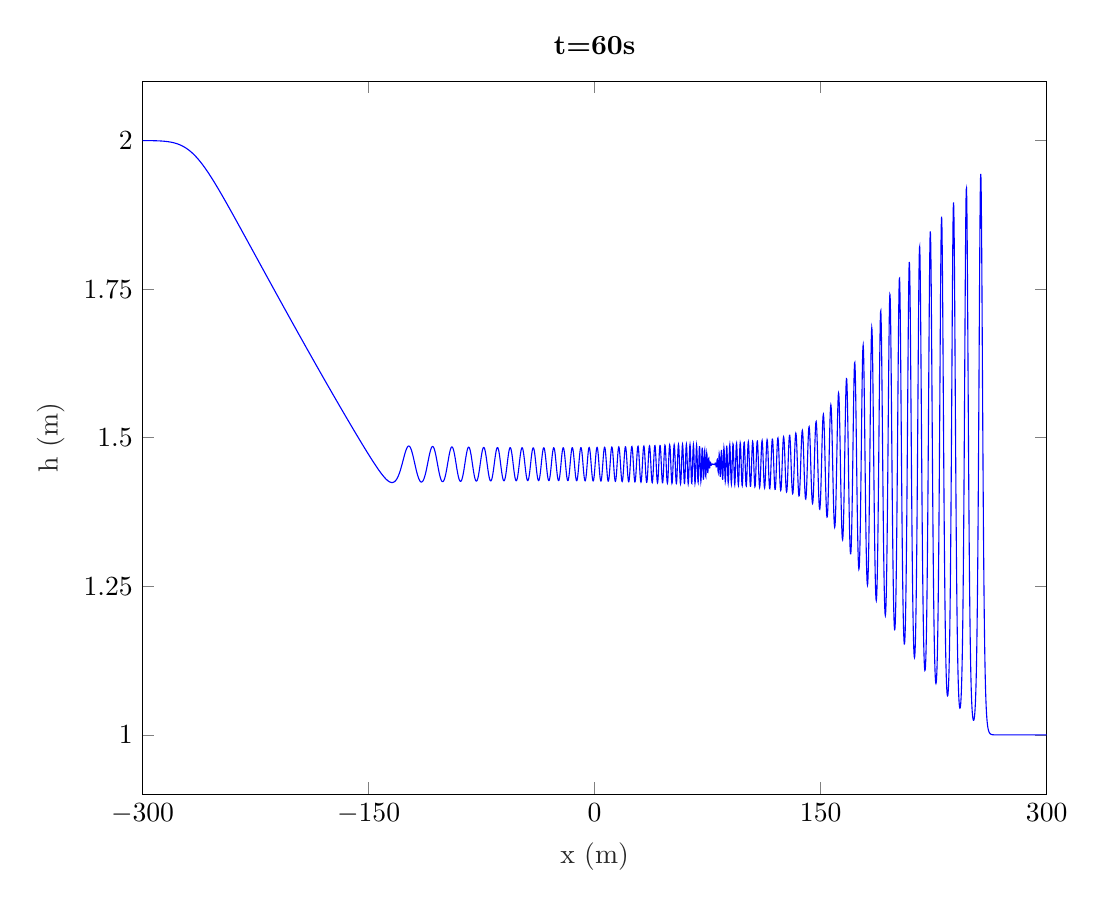
\begin{tikzpicture}

\begin{axis}[%
width=4.521in,
height=3.566in,
at={(0.758in,0.481in)},
scale only axis,
xmin=-300,
xmax=300,
xtick={-300, -150,    0,  150,  300},
xlabel style={font=\color{white!15!black}},
xlabel={x (m)},
ymin=0.9,
ymax=2.1,
ytick={   1, 1.25,  1.5, 1.75,    2},
ylabel style={font=\color{white!15!black}},
ylabel={h (m)},
axis background/.style={fill=white},
title style={font=\bfseries},
title={t=60s}
]
\addplot [color=blue, forget plot]
  table[row sep=crcr]{%
-300.18000900045	2\\
-300.030001500075	2\\
-299.8799939997	1.99990515311427\\
-299.729986499325	1.99990732133151\\
-299.57997899895	1.99990779077288\\
-299.429971498575	1.99990707525083\\
-299.2799639982	1.99990635262908\\
-299.129956497825	1.99990549887404\\
-298.97994899745	1.99990452632624\\
-298.829941497075	1.99990342963956\\
-298.6799339967	1.99990220842728\\
-298.529926496325	1.9999008613263\\
-298.37991899595	1.99989938698292\\
-298.229911495575	1.99989778390072\\
-298.0799039952	1.99989605046134\\
-297.929896494825	1.99989418492101\\
-297.77988899445	1.99989218540962\\
-297.629881494075	1.99989004992973\\
-297.4798739937	1.99988777635538\\
-297.329866493325	1.99988536243086\\
-297.17985899295	1.99988280576947\\
-297.029851492575	1.99988010385217\\
-296.8798439922	1.99987725402618\\
-296.729836491825	1.99987425350348\\
-296.57982899145	1.99987109935935\\
-296.429821491075	1.99986778853073\\
-296.2798139907	1.9998643178146\\
-296.129806490325	1.99986068386625\\
-295.979798989949	1.99985688319751\\
-295.829791489574	1.99985291217495\\
-295.679783989199	1.99984876701796\\
-295.529776488824	1.99984444379684\\
-295.379768988449	1.99983993843076\\
-295.229761488074	1.99983524668574\\
-295.079753987699	1.99983036417251\\
-294.929746487324	1.99982528634435\\
-294.779738986949	1.99982000849489\\
-294.629731486574	1.99981452575581\\
-294.479723986199	1.99980883309455\\
-294.329716485824	1.99980292531188\\
-294.179708985449	1.99979679703955\\
-294.029701485074	1.99979044273777\\
-293.879693984699	1.99978385669273\\
-293.729686484324	1.99977703301399\\
-293.579678983949	1.99976996563194\\
-293.429671483574	1.99976264829511\\
-293.279663983199	1.99975507456751\\
-293.129656482824	1.99974723782588\\
-292.979648982449	1.99973913125696\\
-292.829641482074	1.99973074785467\\
-292.679633981699	1.9997220804173\\
-292.529626481324	1.99971312154465\\
-292.379618980949	1.99970386363513\\
-292.229611480574	1.99969429888285\\
-292.079603980199	1.99968441927469\\
-291.929596479824	1.99967421658731\\
-291.779588979449	1.99966368238421\\
-291.629581479074	1.99965280801269\\
-291.479573978699	1.99964158460087\\
-291.329566478324	1.99963000305462\\
-291.179558977949	1.99961805405457\\
-291.029551477574	1.99960572805303\\
-290.879543977199	1.99959301527096\\
-290.729536476824	1.99957990569491\\
-290.579528976449	1.99956638907398\\
-290.429521476074	1.99955245491678\\
-290.279513975699	1.99953809248837\\
-290.129506475324	1.99952329080728\\
-289.979498974949	1.99950803864248\\
-289.829491474574	1.99949232451036\\
-289.679483974199	1.99947613667184\\
-289.529476473824	1.99945946312935\\
-289.379468973449	1.99944229162397\\
-289.229461473074	1.99942460963253\\
-289.079453972699	1.99940640436479\\
-288.929446472324	1.99938766276061\\
-288.779438971949	1.99936837148724\\
-288.629431471574	1.99934851693658\\
-288.479423971199	1.99932808522257\\
-288.329416470824	1.99930706217858\\
-288.179408970449	1.99928543335487\\
-288.029401470073	1.9992631840162\\
-287.879393969698	1.99924029913936\\
-287.729386469323	1.99921676341093\\
-287.579378968948	1.99919256122503\\
-287.429371468573	1.99916767668121\\
-287.279363968198	1.99914209358237\\
-287.129356467823	1.99911579543284\\
-286.979348967448	1.99908876543654\\
-286.829341467073	1.99906098649524\\
-286.679333966698	1.99903244120694\\
-286.529326466323	1.99900311186437\\
-286.379318965948	1.99897298045358\\
-286.229311465573	1.99894202865277\\
-286.079303965198	1.99891023783107\\
-285.929296464823	1.99887758904766\\
-285.779288964448	1.99884406305088\\
-285.629281464073	1.99880964027757\\
-285.479273963698	1.99877430085255\\
-285.329266463323	1.99873802458826\\
-285.179258962948	1.99870079098455\\
-285.029251462573	1.99866257922869\\
-284.879243962198	1.99862336819551\\
-284.729236461823	1.99858313644772\\
-284.579228961448	1.99854186223649\\
-284.429221461073	1.99849952350215\\
-284.279213960698	1.9984560978751\\
-284.129206460323	1.99841156267696\\
-283.979198959948	1.99836589492191\\
-283.829191459573	1.99831907131826\\
-283.679183959198	1.99827106827019\\
-283.529176458823	1.99822186187978\\
-283.379168958448	1.99817142794926\\
-283.229161458073	1.99811974198343\\
-283.079153957698	1.99806677919241\\
-282.929146457323	1.99801251449459\\
-282.779138956948	1.99795692251979\\
-282.629131456573	1.99789997761279\\
-282.479123956198	1.99784165383696\\
-282.329116455823	1.99778192497827\\
-282.179108955448	1.99772076454957\\
-282.029101455073	1.99765814579499\\
-281.879093954698	1.99759404169482\\
-281.729086454323	1.99752842497048\\
-281.579078953948	1.99746126808992\\
-281.429071453573	1.99739254327314\\
-281.279063953198	1.99732222249816\\
-281.129056452823	1.99725027750715\\
-280.979048952448	1.99717667981286\\
-280.829041452073	1.99710140070544\\
-280.679033951698	1.9970244112594\\
-280.529026451323	1.99694568234096\\
-280.379018950948	1.99686518461568\\
-280.229011450573	1.99678288855631\\
-280.079003950197	1.99669876445103\\
-279.928996449822	1.99661278241191\\
-279.778988949447	1.99652491238368\\
-279.628981449072	1.99643512415278\\
-279.478973948697	1.99634338735671\\
-279.328966448322	1.99624967149365\\
-279.178958947947	1.99615394593238\\
-279.028951447572	1.99605617992245\\
-278.878943947197	1.99595634260465\\
-278.728936446822	1.99585440302175\\
-278.578928946447	1.99575033012948\\
-278.428921446072	1.99564409280785\\
-278.278913945697	1.99553565987261\\
-278.128906445322	1.99542500008709\\
-277.978898944947	1.99531208217419\\
-277.828891444572	1.99519687482869\\
-277.678883944197	1.9950793467297\\
-277.528876443822	1.99495946655348\\
-277.378868943447	1.99483720298634\\
-277.228861443072	1.99471252473786\\
-277.078853942697	1.99458540055421\\
-276.928846442322	1.99445579923182\\
-276.778838941947	1.99432368963106\\
-276.628831441572	1.99418904069025\\
-276.478823941197	1.99405182143978\\
-276.328816440822	1.99391200101635\\
-276.178808940447	1.99376954867743\\
-276.028801440072	1.99362443381581\\
-275.878793939697	1.99347662597431\\
-275.728786439322	1.99332609486059\\
-275.578778938947	1.99317281036205\\
-275.428771438572	1.99301674256083\\
-275.278763938197	1.99285786174891\\
-275.128756437822	1.99269613844327\\
-274.978748937447	1.99253154340104\\
-274.828741437072	1.99236404763479\\
-274.678733936697	1.99219362242776\\
-274.528726436322	1.99202023934915\\
-274.378718935947	1.99184387026939\\
-274.228711435572	1.99166448737536\\
-274.078703935197	1.99148206318566\\
-273.928696434822	1.99129657056574\\
-273.778688934447	1.99110798274303\\
-273.628681434072	1.99091627332194\\
-273.478673933697	1.99072141629881\\
-273.328666433322	1.99052338607676\\
-273.178658932947	1.99032215748035\\
-273.028651432572	1.99011770577015\\
-272.878643932197	1.98991000665719\\
-272.728636431822	1.9896990363171\\
-272.578628931447	1.98948477140427\\
-272.428621431072	1.98926718906562\\
-272.278613930697	1.98904626695424\\
-272.128606430321	1.98882198324282\\
-271.978598929946	1.98859431663675\\
-271.828591429571	1.98836324638705\\
-271.678583929196	1.98812875230296\\
-271.528576428821	1.98789081476424\\
-271.378568928446	1.98764941473323\\
-271.228561428071	1.98740453376649\\
-271.078553927696	1.98715615402618\\
-270.928546427321	1.98690425829109\\
-270.778538926946	1.98664882996725\\
-270.628531426571	1.98638985309825\\
-270.478523926196	1.9861273123751\\
-270.328516425821	1.98586119314576\\
-270.178508925446	1.98559148142419\\
-270.028501425071	1.98531816389906\\
-269.878493924696	1.98504122794194\\
-269.728486424321	1.98476066161516\\
-269.578478923946	1.98447645367911\\
-269.428471423571	1.98418859359914\\
-269.278463923196	1.98389707155204\\
-269.128456422821	1.98360187843188\\
-268.978448922446	1.9833030058556\\
-268.828441422071	1.98300044616791\\
-268.678433921696	1.9826941924458\\
-268.528426421321	1.98238423850254\\
-268.378418920946	1.98207057889114\\
-268.228411420571	1.98175320890733\\
-268.078403920196	1.98143212459201\\
-267.928396419821	1.98110732273323\\
-267.778388919446	1.98077880086757\\
-267.628381419071	1.98044655728108\\
-267.478373918696	1.98011059100967\\
-267.328366418321	1.97977090183895\\
-267.178358917946	1.97942749030361\\
-267.028351417571	1.97908035768623\\
-266.878343917196	1.97872950601563\\
-266.728336416821	1.97837493806462\\
-266.578328916446	1.97801665734733\\
-266.428321416071	1.97765466811599\\
-266.278313915696	1.97728897535718\\
-266.128306415321	1.97691958478767\\
-265.978298914946	1.97654650284966\\
-265.828291414571	1.97616973670562\\
-265.678283914196	1.97578929423261\\
-265.528276413821	1.97540518401614\\
-265.378268913446	1.97501741534359\\
-265.228261413071	1.97462599819709\\
-265.078253912696	1.97423094324611\\
-264.928246412321	1.97383226183945\\
-264.778238911946	1.97342996599694\\
-264.628231411571	1.9730240684006\\
-264.478223911196	1.97261458238553\\
-264.328216410821	1.9722015219303\\
-264.178208910446	1.97178490164705\\
-264.02820141007	1.97136473677113\\
-263.878193909695	1.97094104315046\\
-263.72818640932	1.97051383723453\\
-263.578178908945	1.97008313606307\\
-263.42817140857	1.96964895725441\\
-263.278163908195	1.9692113189935\\
-263.12815640782	1.96877024001975\\
-262.978148907445	1.96832573961448\\
-262.82814140707	1.96787783758818\\
-262.678133906695	1.96742655426754\\
-262.52812640632	1.96697191048223\\
-262.378118905945	1.96651392755145\\
-262.22811140557	1.96605262727032\\
-262.078103905195	1.96558803189611\\
-261.92809640482	1.96512016413424\\
-261.778088904445	1.96464904712417\\
-261.62808140407	1.96417470442519\\
-261.478073903695	1.96369716000201\\
-261.32806640332	1.96321643821036\\
-261.178058902945	1.96273256378236\\
-261.02805140257	1.96224556181195\\
-260.878043902195	1.96175545774023\\
-260.72803640182	1.96126227734066\\
-260.578028901445	1.96076604670437\\
-260.42802140107	1.9602667922254\\
-260.278013900695	1.95976454058591\\
-260.12800640032	1.95925931874145\\
-259.977998899945	1.95875115390624\\
-259.82799139957	1.9582400735385\\
-259.677983899195	1.95772610532583\\
-259.52797639882	1.95720927717067\\
-259.377968898445	1.95668961717582\\
-259.22796139807	1.95616715363005\\
-259.077953897695	1.9556419149939\\
-258.92794639732	1.95511392988544\\
-258.777938896945	1.95458322706633\\
-258.62793139657	1.95404983542788\\
-258.477923896195	1.95351378397735\\
-258.32791639582	1.95297510182436\\
-258.177908895445	1.95243381816751\\
-258.02790139507	1.95188996228114\\
-257.877893894695	1.95134356350231\\
-257.72788639432	1.95079465121795\\
-257.577878893945	1.95024325485221\\
-257.42787139357	1.94968940385409\\
-257.277863893195	1.94913312768519\\
-257.12785639282	1.94857445580777\\
-256.977848892445	1.94801341767298\\
-256.82784139207	1.94745004270936\\
-256.677833891695	1.94688436031159\\
-256.52782639132	1.94631639982948\\
-256.377818890945	1.94574619055719\\
-256.22781139057	1.94517376172276\\
-256.077803890195	1.94459914247784\\
-255.927796389819	1.94402236188776\\
-255.777788889444	1.94344344892177\\
-255.627781389069	1.94286243244364\\
-255.477773888694	1.94227934120251\\
-255.327766388319	1.94169420382397\\
-255.177758887944	1.94110704880146\\
-255.027751387569	1.94051790448794\\
-254.877743887194	1.93992679908786\\
-254.727736386819	1.93933376064933\\
-254.577728886444	1.93873881705668\\
-254.427721386069	1.93814199602318\\
-254.277713885694	1.93754332508416\\
-254.127706385319	1.9369428315903\\
-253.977698884944	1.93634054270125\\
-253.827691384569	1.93573648537954\\
-253.677683884194	1.9351306863847\\
-253.527676383819	1.9345231722677\\
-253.377668883444	1.93391396936566\\
-253.227661383069	1.93330310379679\\
-253.077653882694	1.93269060145563\\
-252.927646382319	1.93207648800851\\
-252.777638881944	1.93146078888932\\
-252.627631381569	1.93084352929547\\
-252.477623881194	1.93022473418415\\
-252.327616380819	1.92960442826881\\
-252.177608880444	1.9289826360159\\
-252.027601380069	1.92835938164182\\
-251.877593879694	1.92773468911012\\
-251.727586379319	1.92710858212895\\
-251.577578878944	1.92648108414867\\
-251.427571378569	1.92585221835978\\
-251.277563878194	1.92522200769096\\
-251.127556377819	1.92459047480739\\
-250.977548877444	1.92395764210922\\
-250.827541377069	1.92332353173035\\
-250.677533876694	1.92268816553723\\
-250.527526376319	1.92205156512803\\
-250.377518875944	1.92141375183188\\
-250.227511375569	1.9207747467083\\
-250.077503875194	1.92013457054687\\
-249.927496374819	1.91949324386704\\
-249.777488874444	1.91885078691802\\
-249.627481374069	1.91820721967898\\
-249.477473873694	1.91756256185929\\
-249.327466373319	1.91691683289893\\
-249.177458872944	1.91627005196911\\
-249.027451372569	1.91562223797291\\
-248.877443872194	1.91497340954618\\
-248.727436371819	1.91432358505847\\
-248.577428871444	1.91367278261413\\
-248.427421371069	1.91302102005355\\
-248.277413870694	1.9123683149544\\
-248.127406370319	1.91171468463317\\
-247.977398869943	1.91106014614661\\
-247.827391369568	1.91040471629344\\
-247.677383869193	1.90974841161599\\
-247.527376368818	1.9090912484021\\
-247.377368868443	1.90843324268697\\
-247.227361368068	1.90777441025516\\
-247.077353867693	1.90711476664262\\
-246.927346367318	1.90645432713886\\
-246.777338866943	1.90579310678912\\
-246.627331366568	1.90513112039662\\
-246.477323866193	1.9044683825249\\
-246.327316365818	1.90380490750017\\
-246.177308865443	1.90314070941375\\
-246.027301365068	1.90247580212454\\
-245.877293864693	1.90181019926152\\
-245.727286364318	1.90114391422632\\
-245.577278863943	1.90047696019582\\
-245.427271363568	1.89980935012475\\
-245.277263863193	1.89914109674837\\
-245.127256362818	1.89847221258513\\
-244.977248862443	1.8978027099394\\
-244.827241362068	1.89713260090418\\
-244.677233861693	1.89646189736387\\
-244.527226361318	1.895790610997\\
-244.377218860943	1.895118753279\\
-244.227211360568	1.89444633548504\\
-244.077203860193	1.89377336869274\\
-243.927196359818	1.89309986378505\\
-243.777188859443	1.89242583145297\\
-243.627181359068	1.8917512821984\\
-243.477173858693	1.89107622633693\\
-243.327166358318	1.89040067400063\\
-243.177158857943	1.88972463514082\\
-243.027151357568	1.88904811953087\\
-242.877143857193	1.88837113676898\\
-242.727136356818	1.88769369628092\\
-242.577128856443	1.88701580732281\\
-242.427121356068	1.8863374789838\\
-242.277113855693	1.88565872018885\\
-242.127106355318	1.88497953970138\\
-241.977098854943	1.884299946126\\
-241.827091354568	1.88361994791114\\
-241.677083854193	1.8829395533517\\
-241.527076353818	1.88225877059169\\
-241.377068853443	1.88157760762682\\
-241.227061353068	1.88089607230707\\
-241.077053852693	1.88021417233922\\
-240.927046352318	1.87953191528943\\
-240.777038851943	1.87884930858571\\
-240.627031351568	1.87816635952038\\
-240.477023851193	1.87748307525252\\
-240.327016350818	1.87679946281041\\
-240.177008850443	1.87611552909392\\
-240.027001350068	1.87543128087682\\
-239.876993849692	1.87474672480916\\
-239.726986349317	1.87406186741956\\
-239.576978848942	1.87337671511746\\
-239.426971348567	1.87269127419539\\
-239.276963848192	1.87200555083113\\
-239.126956347817	1.87131955108997\\
-238.976948847442	1.87063328092674\\
-238.826941347067	1.86994674618804\\
-238.676933846692	1.86925995261425\\
-238.526926346317	1.86857290584159\\
-238.376918845942	1.86788561140418\\
-238.226911345567	1.86719807473597\\
-238.076903845192	1.86651030117274\\
-237.926896344817	1.865822295954\\
-237.776888844442	1.86513406422491\\
-237.626881344067	1.86444561103809\\
-237.476873843692	1.86375694135551\\
-237.326866343317	1.86306806005026\\
-237.176858842942	1.8623789719083\\
-237.026851342567	1.86168968163023\\
-236.876843842192	1.86100019383298\\
-236.726836341817	1.86031051305147\\
-236.576828841442	1.85962064374029\\
-236.426821341067	1.85893059027529\\
-236.276813840692	1.85824035695518\\
-236.126806340317	1.85754994800305\\
-235.976798839942	1.85685936756796\\
-235.826791339567	1.85616861972638\\
-235.676783839192	1.85547770848368\\
-235.526776338817	1.85478663777558\\
-235.376768838442	1.85409541146957\\
-235.226761338067	1.85340403336625\\
-235.076753837692	1.85271250720075\\
-234.926746337317	1.85202083664402\\
-234.776738836942	1.85132902530413\\
-234.626731336567	1.8506370767276\\
-234.476723836192	1.8499449944006\\
-234.326716335817	1.84925278175018\\
-234.176708835442	1.84856044214553\\
-234.026701335067	1.84786797889908\\
-233.876693834692	1.84717539526772\\
-233.726686334317	1.84648269445389\\
-233.576678833942	1.8457898796067\\
-233.426671333567	1.845096953823\\
-233.276663833192	1.84440392014849\\
-233.126656332817	1.84371078157868\\
-232.976648832442	1.84301754105997\\
-232.826641332067	1.84232420149062\\
-232.676633831692	1.84163076572174\\
-232.526626331317	1.84093723655822\\
-232.376618830942	1.84024361675967\\
-232.226611330567	1.83954990904133\\
-232.076603830192	1.83885611607499\\
-231.926596329817	1.83816224048984\\
-231.776588829441	1.83746828487331\\
-231.626581329066	1.83677425177195\\
-231.476573828691	1.83608014369221\\
-231.326566328316	1.83538596310123\\
-231.176558827941	1.8346917124277\\
-231.026551327566	1.83399739406253\\
-230.876543827191	1.83330301035966\\
-230.726536326816	1.83260856363676\\
-230.576528826441	1.83191405617597\\
-230.426521326066	1.83121949022459\\
-230.276513825691	1.83052486799578\\
-230.126506325316	1.82983019166918\\
-229.976498824941	1.82913546339165\\
-229.826491324566	1.82844068527783\\
-229.676483824191	1.82774585941081\\
-229.526476323816	1.82705098784274\\
-229.376468823441	1.82635607259543\\
-229.226461323066	1.8256611156609\\
-229.076453822691	1.82496611900201\\
-228.926446322316	1.82427108455299\\
-228.776438821941	1.82357601421999\\
-228.626431321566	1.82288090988162\\
-228.476423821191	1.82218577338948\\
-228.326416320816	1.82149060656864\\
-228.176408820441	1.82079541121821\\
-228.026401320066	1.82010018911176\\
-227.876393819691	1.81940494199783\\
-227.726386319316	1.8187096716004\\
-227.576378818941	1.81801437961937\\
-227.426371318566	1.81731906773094\\
-227.276363818191	1.81662373758813\\
-227.126356317816	1.81592839082118\\
-226.976348817441	1.81523302903793\\
-226.826341317066	1.81453765382429\\
-226.676333816691	1.81384226674461\\
-226.526326316316	1.8131468693421\\
-226.376318815941	1.81245146313916\\
-226.226311315566	1.81175604963783\\
-226.076303815191	1.81106063032008\\
-225.926296314816	1.81036520664824\\
-225.776288814441	1.80966978006531\\
-225.626281314066	1.80897435199533\\
-225.476273813691	1.8082789238437\\
-225.326266313316	1.80758349699751\\
-225.176258812941	1.80688807282588\\
-225.026251312566	1.80619265268024\\
-224.876243812191	1.80549723789471\\
-224.726236311816	1.80480182978633\\
-224.576228811441	1.80410642965537\\
-224.426221311066	1.80341103878568\\
-224.276213810691	1.8027156584449\\
-224.126206310316	1.80202028988477\\
-223.976198809941	1.80132493434141\\
-223.826191309565	1.80062959303559\\
-223.67618380919	1.79993426717296\\
-223.526176308815	1.79923895794433\\
-223.37616880844	1.79854366652593\\
-223.226161308065	1.79784839407963\\
-223.07615380769	1.7971531417532\\
-222.926146307315	1.79645791068054\\
-222.77613880694	1.7957627019819\\
-222.626131306565	1.79506751676412\\
-222.47612380619	1.79437235612087\\
-222.326116305815	1.79367722113281\\
-222.17610880544	1.79298211286788\\
-222.026101305065	1.79228703238141\\
-221.87609380469	1.79159198071643\\
-221.726086304315	1.79089695890381\\
-221.57607880394	1.79020196796245\\
-221.426071303565	1.78950700889951\\
-221.27606380319	1.78881208271057\\
-221.126056302815	1.78811719037982\\
-220.97604880244	1.78742233288025\\
-220.826041302065	1.78672751117384\\
-220.67603380169	1.78603272621169\\
-220.526026301315	1.78533797893424\\
-220.37601880094	1.7846432702714\\
-220.226011300565	1.78394860114274\\
-220.07600380019	1.78325397245766\\
-219.925996299815	1.78255938511549\\
-219.77598879944	1.78186484000574\\
-219.625981299065	1.78117033800816\\
-219.47597379869	1.78047587999294\\
-219.325966298315	1.77978146682085\\
-219.17595879794	1.77908709934338\\
-219.025951297565	1.77839277840287\\
-218.87594379719	1.77769850483269\\
-218.725936296815	1.77700427945732\\
-218.57592879644	1.77631010309252\\
-218.425921296065	1.77561597654545\\
-218.27591379569	1.77492190061482\\
-218.125906295315	1.77422787609097\\
-217.97589879494	1.77353390375604\\
-217.825891294565	1.77283998438407\\
-217.67588379419	1.77214611874114\\
-217.525876293815	1.77145230758545\\
-217.37586879344	1.77075855166748\\
-217.225861293065	1.77006485173006\\
-217.07585379269	1.76937120850853\\
-216.925846292315	1.76867762273082\\
-216.77583879194	1.76798409511754\\
-216.625831291565	1.76729062638214\\
-216.47582379119	1.76659721723096\\
-216.325816290815	1.76590386836339\\
-216.17580879044	1.76521058047189\\
-216.025801290065	1.76451735424217\\
-215.875793789689	1.76382419035324\\
-215.725786289314	1.76313108947753\\
-215.575778788939	1.76243805228097\\
-215.425771288564	1.76174507942309\\
-215.275763788189	1.76105217155708\\
-215.125756287814	1.76035932932995\\
-214.975748787439	1.75966655338254\\
-214.825741287064	1.75897384434967\\
-214.675733786689	1.75828120286018\\
-214.525726286314	1.75758862953704\\
-214.375718785939	1.75689612499742\\
-214.225711285564	1.75620368985278\\
-214.075703785189	1.75551132470893\\
-213.925696284814	1.75481903016616\\
-213.775688784439	1.75412680681924\\
-213.625681284064	1.75343465525756\\
-213.475673783689	1.75274257606518\\
-213.325666283314	1.75205056982092\\
-213.175658782939	1.75135863709839\\
-213.025651282564	1.75066677846613\\
-212.875643782189	1.7499749944876\\
-212.725636281814	1.74928328572134\\
-212.575628781439	1.74859165272094\\
-212.425621281064	1.7479000960352\\
-212.275613780689	1.74720861620813\\
-212.125606280314	1.74651721377904\\
-211.975598779939	1.74582588928262\\
-211.825591279564	1.74513464324898\\
-211.675583779189	1.74444347620371\\
-211.525576278814	1.74375238866797\\
-211.375568778439	1.74306138115853\\
-211.225561278064	1.74237045418781\\
-211.075553777689	1.74167960826399\\
-210.925546277314	1.74098884389102\\
-210.775538776939	1.74029816156871\\
-210.625531276564	1.73960756179278\\
-210.475523776189	1.73891704505489\\
-210.325516275814	1.73822661184273\\
-210.175508775439	1.73753626264005\\
-210.025501275064	1.73684599792673\\
-209.875493774689	1.73615581817882\\
-209.725486274314	1.73546572386861\\
-209.575478773939	1.73477571546464\\
-209.425471273564	1.73408579343182\\
-209.275463773189	1.7333959582314\\
-209.125456272814	1.73270621032109\\
-208.975448772439	1.73201655015505\\
-208.825441272064	1.731326978184\\
-208.675433771689	1.73063749485519\\
-208.525426271314	1.72994810061253\\
-208.375418770939	1.72925879589658\\
-208.225411270564	1.72856958114459\\
-208.075403770189	1.72788045679061\\
-207.925396269813	1.72719142326546\\
-207.775388769438	1.72650248099681\\
-207.625381269063	1.72581363040922\\
-207.475373768688	1.72512487192419\\
-207.325366268313	1.72443620596018\\
-207.175358767938	1.72374763293268\\
-207.025351267563	1.72305915325422\\
-206.875343767188	1.72237076733444\\
-206.725336266813	1.72168247558011\\
-206.575328766438	1.72099427839518\\
-206.425321266063	1.72030617618081\\
-206.275313765688	1.71961816933545\\
-206.125306265313	1.71893025825479\\
-205.975298764938	1.71824244333189\\
-205.825291264563	1.71755472495718\\
-205.675283764188	1.71686710351847\\
-205.525276263813	1.71617957940105\\
-205.375268763438	1.71549215298766\\
-205.225261263063	1.71480482465857\\
-205.075253762688	1.7141175947916\\
-204.925246262313	1.71343046376216\\
-204.775238761938	1.71274343194327\\
-204.625231261563	1.71205649970562\\
-204.475223761188	1.71136966741759\\
-204.325216260813	1.71068293544528\\
-204.175208760438	1.70999630415254\\
-204.025201260063	1.70930977390102\\
-203.875193759688	1.7086233450502\\
-203.725186259313	1.7079370179574\\
-203.575178758938	1.70725079297784\\
-203.425171258563	1.70656467046465\\
-203.275163758188	1.70587865076893\\
-203.125156257813	1.70519273423974\\
-202.975148757438	1.70450692122418\\
-202.825141257063	1.70382121206735\\
-202.675133756688	1.70313560711248\\
-202.525126256313	1.70245010670086\\
-202.375118755938	1.70176471117195\\
-202.225111255563	1.70107942086334\\
-202.075103755188	1.70039423611084\\
-201.925096254813	1.69970915724847\\
-201.775088754438	1.69902418460852\\
-201.625081254063	1.69833931852152\\
-201.475073753688	1.69765455931635\\
-201.325066253313	1.69696990732021\\
-201.175058752938	1.69628536285868\\
-201.025051252563	1.69560092625569\\
-200.875043752188	1.69491659783365\\
-200.725036251813	1.69423237791336\\
-200.575028751438	1.69354826681414\\
-200.425021251063	1.69286426485379\\
-200.275013750688	1.69218037234864\\
-200.125006250313	1.69149658961359\\
-199.974998749937	1.6908129169621\\
-199.824991249562	1.69012935470624\\
-199.674983749187	1.68944590315674\\
-199.524976248812	1.68876256262296\\
-199.374968748437	1.68807933341296\\
-199.224961248062	1.68739621583352\\
-199.074953747687	1.68671321019015\\
-198.924946247312	1.68603031678711\\
-198.774938746937	1.68534753592746\\
-198.624931246562	1.68466486791308\\
-198.474923746187	1.68398231304468\\
-198.324916245812	1.68329987162183\\
-198.174908745437	1.68261754394299\\
-198.024901245062	1.68193533030554\\
-197.874893744687	1.68125323100579\\
-197.724886244312	1.68057124633901\\
-197.574878743937	1.67988937659947\\
-197.424871243562	1.67920762208043\\
-197.274863743187	1.67852598307421\\
-197.124856242812	1.67784445987216\\
-196.974848742437	1.67716305276474\\
-196.824841242062	1.6764817620415\\
-196.674833741687	1.67580058799113\\
-196.524826241312	1.67511953090147\\
-196.374818740937	1.67443859105953\\
-196.224811240562	1.67375776875155\\
-196.074803740187	1.67307706426298\\
-195.924796239812	1.67239647787851\\
-195.774788739437	1.67171600988212\\
-195.624781239062	1.67103566055708\\
-195.474773738687	1.67035543018599\\
-195.324766238312	1.66967531905078\\
-195.174758737937	1.66899532743275\\
-195.024751237562	1.66831545561263\\
-194.874743737187	1.6676357038705\\
-194.724736236812	1.66695607248593\\
-194.574728736437	1.66627656173793\\
-194.424721236062	1.66559717190502\\
-194.274713735687	1.66491790326521\\
-194.124706235312	1.66423875609603\\
-193.974698734937	1.66355973067459\\
-193.824691234562	1.66288082727759\\
-193.674683734187	1.6622020461813\\
-193.524676233812	1.66152338766166\\
-193.374668733437	1.66084485199423\\
-193.224661233062	1.66016643945427\\
-193.074653732687	1.65948815031671\\
-192.924646232312	1.65880998485623\\
-192.774638731937	1.65813194334725\\
-192.624631231562	1.65745402606397\\
-192.474623731187	1.65677623328037\\
-192.324616230812	1.65609856527027\\
-192.174608730437	1.65542102230731\\
-192.024601230062	1.65474360466502\\
-191.874593729686	1.65406631261682\\
-191.724586229311	1.65338914643604\\
-191.574578728936	1.65271210639598\\
-191.424571228561	1.65203519276986\\
-191.274563728186	1.65135840583094\\
-191.124556227811	1.65068174585247\\
-190.974548727436	1.65000521310776\\
-190.824541227061	1.64932880787018\\
-190.674533726686	1.64865253041319\\
-190.524526226311	1.64797638101038\\
-190.374518725936	1.64730035993549\\
-190.224511225561	1.64662446746241\\
-190.074503725186	1.64594870386525\\
-189.924496224811	1.64527306941834\\
-189.774488724436	1.64459756439624\\
-189.624481224061	1.64392218907382\\
-189.474473723686	1.64324694372624\\
-189.324466223311	1.64257182862898\\
-189.174458722936	1.6418968440579\\
-189.024451222561	1.64122199028922\\
-188.874443722186	1.64054726759961\\
-188.724436221811	1.63987267626615\\
-188.574428721436	1.6391982165664\\
-188.424421221061	1.63852388877843\\
-188.274413720686	1.63784969318081\\
-188.124406220311	1.63717563005271\\
-187.974398719936	1.63650169967385\\
-187.824391219561	1.63582790232457\\
-187.674383719186	1.63515423828586\\
-187.524376218811	1.6344807078394\\
-187.374368718436	1.63380731126756\\
-187.224361218061	1.63313404885344\\
-187.074353717686	1.63246092088093\\
-186.924346217311	1.63178792763469\\
-186.774338716936	1.63111506940023\\
-186.624331216561	1.63044234646393\\
-186.474323716186	1.62976975911304\\
-186.324316215811	1.62909730763577\\
-186.174308715436	1.62842499232125\\
-186.024301215061	1.62775281345966\\
-185.874293714686	1.62708077134215\\
-185.724286214311	1.62640886626097\\
-185.574278713936	1.62573709850946\\
-185.424271213561	1.62506546838209\\
-185.274263713186	1.62439397617452\\
-185.124256212811	1.62372262218358\\
-184.974248712436	1.62305140670736\\
-184.824241212061	1.62238033004524\\
-184.674233711686	1.6217093924979\\
-184.524226211311	1.62103859436738\\
-184.374218710936	1.62036793595712\\
-184.224211210561	1.61969741757198\\
-184.074203710186	1.61902703951832\\
-183.92419620981	1.61835680210397\\
-183.774188709435	1.61768670563835\\
-183.62418120906	1.61701675043246\\
-183.474173708685	1.61634693679895\\
-183.32416620831	1.61567726505214\\
-183.174158707935	1.61500773550806\\
-183.02415120756	1.61433834848454\\
-182.874143707185	1.61366910430119\\
-182.72413620681	1.61300000327951\\
-182.574128706435	1.61233104574288\\
-182.42412120606	1.61166223201663\\
-182.274113705685	1.61099356242812\\
-182.12410620531	1.61032503730671\\
-181.974098704935	1.60965665698388\\
-181.82409120456	1.60898842179327\\
-181.674083704185	1.60832033207069\\
-181.52407620381	1.6076523881542\\
-181.374068703435	1.60698459038418\\
-181.22406120306	1.60631693910335\\
-181.074053702685	1.60564943465684\\
-180.92404620231	1.60498207739224\\
-180.774038701935	1.60431486765967\\
-180.62403120156	1.6036478058118\\
-180.474023701185	1.60298089220397\\
-180.32401620081	1.60231412719419\\
-180.174008700435	1.60164751114322\\
-180.02400120006	1.60098104441464\\
-179.873993699685	1.60031472737493\\
-179.72398619931	1.59964856039347\\
-179.573978698935	1.59898254384267\\
-179.42397119856	1.598316678098\\
-179.273963698185	1.59765096353807\\
-179.12395619781	1.59698540054471\\
-178.973948697435	1.596319989503\\
-178.82394119706	1.59565473080139\\
-178.673933696685	1.59498962483172\\
-178.52392619631	1.59432467198935\\
-178.373918695935	1.59365987267319\\
-178.22391119556	1.5929952272858\\
-178.073903695185	1.59233073623345\\
-177.92389619481	1.59166639992623\\
-177.773888694435	1.59100221877809\\
-177.62388119406	1.59033819320696\\
-177.473873693685	1.58967432363481\\
-177.32386619331	1.58901061048774\\
-177.173858692935	1.58834705419609\\
-177.02385119256	1.58768365519448\\
-176.873843692185	1.58702041392196\\
-176.72383619181	1.58635733082207\\
-176.573828691435	1.58569440634292\\
-176.42382119106	1.58503164093734\\
-176.273813690685	1.58436903506291\\
-176.123806190309	1.58370658918214\\
-175.973798689934	1.58304430376249\\
-175.823791189559	1.58238217927654\\
-175.673783689184	1.58172021620206\\
-175.523776188809	1.58105841502215\\
-175.373768688434	1.58039677622532\\
-175.223761188059	1.57973530030563\\
-175.073753687684	1.57907398776279\\
-174.923746187309	1.57841283910229\\
-174.773738686934	1.57775185483552\\
-174.623731186559	1.57709103547989\\
-174.473723686184	1.57643038155899\\
-174.323716185809	1.57576989360265\\
-174.173708685434	1.57510957214715\\
-174.023701185059	1.57444941773531\\
-173.873693684684	1.57378943091664\\
-173.723686184309	1.5731296122475\\
-173.573678683934	1.57246996229122\\
-173.423671183559	1.57181048161825\\
-173.273663683184	1.57115117080636\\
-173.123656182809	1.57049203044073\\
-172.973648682434	1.56983306111414\\
-172.823641182059	1.56917426342716\\
-172.673633681684	1.56851563798827\\
-172.523626181309	1.56785718541405\\
-172.373618680934	1.56719890632938\\
-172.223611180559	1.56654080136758\\
-172.073603680184	1.56588287117062\\
-171.923596179809	1.56522511638929\\
-171.773588679434	1.56456753768342\\
-171.623581179059	1.56391013572205\\
-171.473573678684	1.56325291118364\\
-171.323566178309	1.56259586475629\\
-171.173558677934	1.56193899713795\\
-171.023551177559	1.56128230903661\\
-170.873543677184	1.56062580117056\\
-170.723536176809	1.55996947426858\\
-170.573528676434	1.55931332907021\\
-170.423521176059	1.55865736632599\\
-170.273513675684	1.55800158679765\\
-170.123506175309	1.55734599125844\\
-169.973498674934	1.55669058049335\\
-169.823491174559	1.55603535529935\\
-169.673483674184	1.55538031648571\\
-169.523476173809	1.55472546487424\\
-169.373468673434	1.55407080129962\\
-169.223461173059	1.55341632660963\\
-169.073453672684	1.55276204166552\\
-168.923446172309	1.55210794734226\\
-168.773438671934	1.5514540445289\\
-168.623431171559	1.55080033412886\\
-168.473423671184	1.5501468170603\\
-168.323416170809	1.54949349425642\\
-168.173408670434	1.54884036666584\\
-168.023401170058	1.54818743525298\\
-167.873393669683	1.54753470099837\\
-167.723386169308	1.54688216489908\\
-167.573378668933	1.54622982796912\\
-167.423371168558	1.54557769123977\\
-167.273363668183	1.54492575576007\\
-167.123356167808	1.54427402259723\\
-166.973348667433	1.543622492837\\
-166.823341167058	1.54297116758421\\
-166.673333666683	1.54232004796316\\
-166.523326166308	1.54166913511812\\
-166.373318665933	1.54101843021383\\
-166.223311165558	1.54036793443595\\
-166.073303665183	1.53971764899164\\
-165.923296164808	1.53906757511002\\
-165.773288664433	1.53841771404277\\
-165.623281164058	1.53776806706464\\
-165.473273663683	1.53711863547405\\
-165.323266163308	1.53646942059369\\
-165.173258662933	1.53582042377108\\
-165.023251162558	1.53517164637927\\
-164.873243662183	1.5345230898174\\
-164.723236161808	1.53387475551143\\
-164.573228661433	1.53322664491477\\
-164.423221161058	1.53257875950901\\
-164.273213660683	1.53193110080465\\
-164.123206160308	1.53128367034179\\
-163.973198659933	1.53063646969095\\
-163.823191159558	1.52998950045385\\
-163.673183659183	1.5293427642642\\
-163.523176158808	1.52869626278854\\
-163.373168658433	1.5280499977271\\
-163.223161158058	1.52740397081472\\
-163.073153657683	1.5267581838217\\
-162.923146157308	1.5261126385548\\
-162.773138656933	1.52546733685819\\
-162.623131156558	1.52482228061442\\
-162.473123656183	1.52417747174552\\
-162.323116155808	1.52353291221398\\
-162.173108655433	1.52288860402393\\
-162.023101155058	1.52224454922218\\
-161.873093654683	1.52160074989949\\
-161.723086154308	1.52095720819167\\
-161.573078653933	1.52031392628088\\
-161.423071153558	1.51967090639692\\
-161.273063653183	1.51902815081849\\
-161.123056152808	1.51838566187462\\
-160.973048652433	1.51774344194602\\
-160.823041152058	1.5171014934666\\
-160.673033651683	1.51645981892488\\
-160.523026151308	1.51581842086561\\
-160.373018650933	1.51517730189134\\
-160.223011150558	1.51453646466407\\
-160.073003650182	1.51389591190696\\
-159.922996149807	1.51325564640607\\
-159.772988649432	1.51261567101222\\
-159.622981149057	1.51197598864283\\
-159.472973648682	1.51133660228387\\
-159.322966148307	1.51069751499188\\
-159.172958647932	1.51005872989604\\
-159.022951147557	1.50942025020031\\
-158.872943647182	1.50878207918563\\
-158.722936146807	1.50814422021224\\
-158.572928646432	1.50750667672204\\
-158.422921146057	1.50686945224103\\
-158.272913645682	1.50623255038186\\
-158.122906145307	1.50559597484642\\
-157.972898644932	1.50495972942861\\
-157.822891144557	1.50432381801709\\
-157.672883644182	1.50368824459823\\
-157.522876143807	1.50305301325906\\
-157.372868643432	1.50241812819046\\
-157.222861143057	1.5017835936903\\
-157.072853642682	1.50114941416684\\
-156.922846142307	1.50051559414213\\
-156.772838641932	1.49988213825565\\
-156.622831141557	1.49924905126793\\
-156.472823641182	1.49861633806446\\
-156.322816140807	1.49798400365966\\
-156.172808640432	1.49735205320093\\
-156.022801140057	1.49672049197299\\
-155.872793639682	1.49608932540229\\
-155.722786139307	1.49545855906155\\
-155.572778638932	1.49482819867459\\
-155.422771138557	1.49419825012116\\
-155.272763638182	1.49356871944214\\
-155.122756137807	1.49293961284478\\
-154.972748637432	1.49231093670821\\
-154.822741137057	1.49168269758914\\
-154.672733636682	1.49105490222779\\
-154.522726136307	1.49042755755397\\
-154.372718635932	1.4898006706935\\
-154.222711135557	1.4891742489748\\
-154.072703635182	1.48854829993571\\
-153.922696134807	1.48792283133067\\
-153.772688634432	1.48729785113802\\
-153.622681134057	1.48667336756775\\
-153.472673633682	1.48604938906942\\
-153.322666133307	1.48542592434042\\
-153.172658632932	1.48480298233459\\
-153.022651132557	1.48418057227111\\
-152.872643632182	1.48355870364381\\
-152.722636131807	1.48293738623072\\
-152.572628631432	1.48231663010416\\
-152.422621131057	1.48169644564109\\
-152.272613630682	1.48107684353389\\
-152.122606130307	1.48045783480167\\
-151.972598629931	1.47983943080186\\
-151.822591129556	1.47922164324239\\
-151.672583629181	1.47860448419433\\
-151.522576128806	1.47798796610495\\
-151.372568628431	1.47737210181143\\
-151.222561128056	1.47675690455501\\
-151.072553627681	1.47614238799579\\
-150.922546127306	1.47552856622806\\
-150.772538626931	1.47491545379632\\
-150.622531126556	1.47430306571187\\
-150.472523626181	1.47369141747014\\
-150.322516125806	1.47308052506868\\
-150.172508625431	1.47247040502592\\
-150.022501125056	1.47186107440069\\
-149.872493624681	1.47125255081249\\
-149.722486124306	1.47064485246268\\
-149.572478623931	1.47003799815649\\
-149.422471123556	1.46943200732594\\
-149.272463623181	1.4688269000537\\
-149.122456122806	1.46822269709797\\
-148.972448622431	1.46761941991839\\
-148.822441122056	1.46701709070299\\
-148.672433621681	1.46641573239632\\
-148.522426121306	1.4658153687287\\
-148.372418620931	1.46521602424673\\
-148.222411120556	1.46461772434507\\
-148.072403620181	1.46402049529955\\
-147.922396119806	1.46342436430167\\
-147.772388619431	1.46282935949459\\
-147.622381119056	1.46223551001053\\
-147.472373618681	1.46164284600991\\
-147.322366118306	1.46105139872201\\
-147.172358617931	1.46046120048739\\
-147.022351117556	1.45987228480216\\
-146.872343617181	1.45928468636402\\
-146.722336116806	1.45869844112038\\
-146.572328616431	1.45811358631839\\
-146.422321116056	1.45753016055719\\
-146.272313615681	1.45694820384239\\
-146.122306115306	1.45636775764273\\
-145.972298614931	1.45578886494933\\
-145.822291114556	1.45521157033734\\
-145.672283614181	1.45463592003021\\
-145.522276113806	1.45406196196676\\
-145.372268613431	1.45348974587105\\
-145.222261113056	1.45291932332519\\
-145.072253612681	1.4523507478453\\
-144.922246112306	1.45178407496062\\
-144.772238611931	1.45121936229604\\
-144.622231111556	1.45065666965804\\
-144.472223611181	1.45009605912432\\
-144.322216110806	1.44953759513711\\
-144.172208610431	1.44898134460053\\
-144.022201110056	1.4484273769819\\
-143.87219360968	1.44787576441737\\
-143.722186109305	1.44732658182188\\
-143.57217860893	1.4467799070038\\
-143.422171108555	1.44623582078412\\
-143.27216360818	1.44569440712078\\
-143.122156107805	1.44515575323791\\
-142.97214860743	1.44461994976045\\
-142.822141107055	1.44408709085422\\
-142.67213360668	1.4435572743716\\
-142.522126106305	1.44303060200314\\
-142.37211860593	1.44250717943516\\
-142.222111105555	1.44198711651356\\
-142.07210360518	1.44147052741415\\
-141.922096104805	1.44095753081954\\
-141.77208860443	1.44044825010288\\
-141.622081104055	1.43994281351863\\
-141.47207360368	1.4394413544005\\
-141.322066103305	1.43894401136684\\
-141.17205860293	1.43845092853352\\
-141.022051102555	1.43796225573461\\
-140.87204360218	1.43747814875094\\
-140.722036101805	1.4369987695467\\
-140.57202860143	1.43652428651418\\
-140.422021101055	1.4360548747269\\
-140.27201360068	1.43559071620101\\
-140.122006100305	1.43513200016522\\
-139.97199859993	1.4346789233392\\
-139.821991099555	1.43423169022048\\
-139.67198359918	1.43379051337991\\
-139.521976098805	1.43335561376544\\
-139.37196859843	1.43292722101426\\
-139.221961098055	1.4325055737731\\
-139.07195359768	1.43209092002643\\
-138.921946097305	1.43168351743232\\
-138.77193859693	1.43128363366549\\
-138.621931096555	1.4308915467673\\
-138.47192359618	1.43050754550196\\
-138.321916095805	1.43013192971838\\
-138.17190859543	1.42976501071697\\
-138.021901095055	1.42940711162034\\
-137.87189359468	1.42905856774719\\
-137.721886094305	1.42871972698784\\
-137.57187859393	1.42839095018036\\
-137.421871093555	1.42807261148573\\
-137.27186359318	1.42776509876014\\
-137.121856092805	1.42746881392274\\
-136.97184859243	1.42718417331652\\
-136.821841092055	1.4269116080599\\
-136.67183359168	1.42665156438638\\
-136.521826091305	1.42640450396923\\
-136.37181859093	1.42617090422776\\
-136.221811090555	1.42595125861169\\
-136.07180359018	1.42574607685932\\
-135.921796089805	1.42555588522517\\
-135.771788589429	1.42538122667212\\
-135.621781089054	1.4252226610227\\
-135.471773588679	1.4250807650635\\
-135.321766088304	1.42495613259657\\
-135.171758587929	1.42484937443059\\
-135.021751087554	1.42476111830433\\
-134.871743587179	1.42469200873444\\
-134.721736086804	1.42464270677783\\
-134.571728586429	1.42461389229207\\
-134.421721086054	1.42460635882282\\
-134.271713585679	1.42462050010228\\
-134.121706085304	1.42465735628306\\
-133.971698584929	1.42471755804193\\
-133.821691084554	1.42480185455098\\
-133.671683584179	1.42491100716511\\
-133.521676083804	1.42504578677279\\
-133.371668583429	1.42520697356243\\
-133.221661083054	1.42539535457117\\
-133.071653582679	1.42561172211989\\
-132.921646082304	1.42585687144221\\
-132.771638581929	1.42613159827404\\
-132.621631081554	1.42643669614031\\
-132.471623581179	1.42677295323433\\
-132.321616080804	1.42714114920937\\
-132.171608580429	1.42754205149052\\
-132.021601080054	1.42797641100877\\
-131.871593579679	1.42844495835341\\
-131.721586079304	1.42894839834694\\
-131.571578578929	1.42948740542327\\
-131.421571078554	1.43006261789721\\
-131.271563578179	1.43067463179967\\
-131.121556077804	1.4313239948885\\
-130.971548577429	1.43201119949402\\
-130.821541077054	1.43273667544097\\
-130.671533576679	1.43350078244589\\
-130.521526076304	1.43430380196114\\
-130.371518575929	1.43514592881339\\
-130.221511075554	1.4360272623855\\
-130.071503575179	1.43694779749421\\
-129.921496074804	1.43790741489594\\
-129.771488574429	1.43890587171707\\
-129.621481074054	1.43994279152279\\
-129.471473573679	1.441017654208\\
-129.321466073304	1.44212978623621\\
-129.171458572929	1.44327835030422\\
-129.021451072554	1.44446233570393\\
-128.871443572179	1.44568054866704\\
-128.721436071804	1.44693160298932\\
-128.571428571429	1.44821391152868\\
-128.421421071054	1.44952567794864\\
-128.271413570679	1.45086488950427\\
-128.121406070304	1.45222931083832\\
-127.971398569929	1.4536164787012\\
-127.821391069553	1.45502369823496\\
-127.671383569178	1.45644804062143\\
-127.521376068803	1.45788634244532\\
-127.371368568428	1.45933520691861\\
-127.221361068053	1.46079100719914\\
-127.071353567678	1.46224989175084\\
-126.921346067303	1.46370779224942\\
-126.771338566928	1.46516043381\\
-126.621331066553	1.46660334780428\\
-126.471323566178	1.46803188752223\\
-126.321316065803	1.46944124622093\\
-126.171308565428	1.47082647818232\\
-126.021301065053	1.47218252234422\\
-125.871293564678	1.47350422847277\\
-125.721286064303	1.47478638601406\\
-125.571278563928	1.47602375507509\\
-125.421271063553	1.47721109966333\\
-125.271263563178	1.47834322270792\\
-125.121256062803	1.47941500257562\\
-124.971248562428	1.48042143082774\\
-124.821241062053	1.48135765068851\\
-124.671233561678	1.4822189958203\\
-124.521226061303	1.48300102901877\\
-124.371218560928	1.48369958017703\\
-124.221211060553	1.48431078316704\\
-124.071203560178	1.48483111107394\\
-123.921196059803	1.48525740916482\\
-123.771188559428	1.48558692538631\\
-123.621181059053	1.48581733759212\\
-123.471173558678	1.48594674702261\\
-123.321166058303	1.48597335081882\\
-123.171158557928	1.48589762524896\\
-123.021151057553	1.48571775289284\\
-122.871143557178	1.48543429432053\\
-122.721136056803	1.48504786866328\\
-122.571128556428	1.48455960238532\\
-122.421121056053	1.48397109833568\\
-122.271113555678	1.48328446770943\\
-122.121106055303	1.482502277941\\
-121.971098554928	1.48162755156522\\
-121.821091054553	1.48066373392627\\
-121.671083554178	1.47961466820077\\
-121.521076053803	1.4784845649052\\
-121.371068553428	1.47727796513077\\
-121.221061053053	1.47599971354113\\
-121.071053552678	1.47465491138909\\
-120.921046052303	1.47324888895275\\
-120.771038551928	1.47178716182696\\
-120.621031051553	1.4702753941686\\
-120.471023551178	1.46871936488181\\
-120.321016050803	1.46712492595736\\
-120.171008550428	1.46549797300878\\
-120.021001050052	1.46384440842163\\
-119.870993549677	1.4621701118209\\
-119.720986049302	1.46048091118482\\
-119.570978548927	1.4587825553429\\
-119.420971048552	1.45708069147309\\
-119.270963548177	1.45538084242654\\
-119.120956047802	1.45368838936061\\
-118.970948547427	1.45200855492423\\
-118.820941047052	1.4503463907526\\
-118.670933546677	1.4487067665589\\
-118.520926046302	1.44709436189649\\
-118.370918545927	1.44551366089199\\
-118.220911045552	1.44396894783447\\
-118.070903545177	1.44246430647456\\
-117.920896044802	1.44100361946195\\
-117.770888544427	1.43959057079351\\
-117.620881044052	1.43822864868392\\
-117.470873543677	1.43692115001558\\
-117.320866043302	1.43567118588366\\
-117.170858542927	1.43448168738811\\
-117.020851042552	1.43335541283194\\
-116.870843542177	1.43229495435744\\
-116.720836041802	1.43130274526878\\
-116.570828541427	1.43038106722384\\
-116.420821041052	1.42953205716861\\
-116.270813540677	1.42875771388067\\
-116.120806040302	1.4280599040924\\
-115.970798539927	1.42744036769662\\
-115.820791039552	1.42690072239106\\
-115.670783539177	1.42644246735098\\
-115.520776038802	1.42606698551893\\
-115.370768538427	1.4257755451788\\
-115.220761038052	1.42556929977955\\
-115.070753537677	1.42544929652939\\
-114.920746037302	1.42541685722156\\
-114.770738536927	1.42547152395293\\
-114.620731036552	1.42561522453674\\
-114.470723536177	1.42584807362637\\
-114.320716035802	1.42617045766029\\
-114.170708535427	1.42658260051091\\
-114.020701035052	1.42708457258552\\
-113.870693534677	1.42767625463909\\
-113.720686034302	1.42835732920425\\
-113.570678533927	1.42912727344207\\
-113.420671033552	1.42998532630015\\
-113.270663533177	1.43093048066567\\
-113.120656032802	1.43196145993964\\
-112.970648532427	1.43307669093575\\
-112.820641032052	1.4342742972262\\
-112.670633531677	1.43555206222785\\
-112.520626031302	1.43690741062767\\
-112.370618530927	1.43833740203019\\
-112.220611030552	1.4398386889634\\
-112.070603530176	1.44140750683335\\
-111.920596029801	1.44303966904694\\
-111.770588529426	1.44473053001127\\
-111.620581029051	1.44647498486162\\
-111.470573528676	1.44826746753705\\
-111.320566028301	1.45010192968913\\
-111.170558527926	1.45197185192986\\
-111.020551027551	1.45387024866283\\
-110.870543527176	1.45578967165947\\
-110.720536026801	1.45772223542651\\
-110.570528526426	1.45965963387844\\
-110.420521026051	1.46159317355951\\
-110.270513525676	1.46351381631532\\
-110.120506025301	1.46541221256613\\
-109.970498524926	1.4672787641529\\
-109.820491024551	1.46910368606809\\
-109.670483524176	1.47087705932993\\
-109.520476023801	1.47258891829561\\
-109.370468523426	1.4742293293586\\
-109.220461023051	1.47578846273678\\
-109.070453522676	1.4772566944765\\
-108.920446022301	1.47862469516547\\
-108.770438521926	1.47988351488745\\
-108.620431021551	1.4810246861544\\
-108.470423521176	1.48204031188286\\
-108.320416020801	1.48292315221701\\
-108.170408520426	1.48366671345881\\
-108.020401020051	1.48426532154362\\
-107.870393519676	1.48471419671658\\
-107.720386019301	1.48500951515516\\
-107.570378518926	1.48514938785861\\
-107.420371018551	1.48512901097012\\
-107.270363518176	1.48495114094439\\
-107.120356017801	1.48461460007676\\
-106.970348517426	1.48412107341017\\
-106.820341017051	1.48347312117405\\
-106.670333516676	1.48267435709084\\
-106.520326016301	1.48172941420698\\
-106.370318515926	1.4806439017033\\
-106.220311015551	1.47942433811166\\
-106.070303515176	1.47807809065863\\
-105.920296014801	1.47661329689754\\
-105.770288514426	1.47503878214409\\
-105.620281014051	1.47336397499324\\
-105.470273513676	1.47159881415891\\
-105.320266013301	1.46975365916704\\
-105.170258512926	1.46783919916031\\
-105.020251012551	1.46586635811408\\
-104.870243512176	1.4638462090503\\
-104.720236011801	1.46178989328959\\
-104.570228511426	1.45970853579464\\
-104.420221011051	1.4576131712155\\
-104.270213510676	1.45551468288664\\
-104.120206010301	1.45342373398452\\
-103.970198509925	1.45135071596873\\
-103.82019100955	1.44930570678135\\
-103.670183509175	1.44729842543072\\
-103.5201760088	1.44533819991918\\
-103.370168508425	1.44343394398346\\
-103.22016100805	1.44159413417751\\
-103.070153507675	1.43982679624898\\
-102.9201460073	1.43813949576138\\
-102.770138506925	1.43653933166336\\
-102.62013100655	1.43503293726661\\
-102.470123506175	1.43362647977107\\
-102.3201160058	1.43232566237493\\
-102.170108505425	1.43113573236501\\
-102.02010100505	1.43006148900099\\
-101.870093504675	1.4291072857834\\
-101.7200860043	1.42827703739694\\
-101.570078503925	1.42757422893676\\
-101.42007100355	1.42700191713986\\
-101.270063503175	1.42656273112975\\
-101.1200560028	1.42625887582374\\
-100.970048502425	1.42609216834322\\
-100.82004100205	1.4260644842659\\
-100.670033501675	1.42617491321914\\
-100.5200260013	1.42642577759252\\
-100.370018500925	1.42681642851748\\
-100.22001100055	1.42734636313653\\
-100.070003500175	1.42801457586988\\
-99.9199959998	1.42881953123089\\
-99.769988499425	1.429759141499\\
-99.6199809990499	1.43083074175809\\
-99.4699734986749	1.43203105673399\\
-99.3199659982999	1.43335617174566\\
-99.1699584979249	1.43480150753439\\
-99.0199509975499	1.43636178802243\\
-98.8699434971749	1.43803101424172\\
-98.7199359967998	1.43980244751841\\
-98.5699284964248	1.44166858118756\\
-98.4199209960498	1.44362112829138\\
-98.2699134956748	1.44565101724908\\
-98.1199059952998	1.44774839021799\\
-97.9698984949247	1.44990261474333\\
-97.8198909945497	1.4521023026943\\
-97.6698834941747	1.45433533640251\\
-97.5198759937997	1.45658891580157\\
-97.3698684934247	1.45884961805224\\
-97.2198609930497	1.4611034666074\\
-97.0698534926746	1.46333601424891\\
-96.9198459922996	1.46553244084128\\
-96.7698384919246	1.46767767185785\\
-96.6198309915496	1.46975650195505\\
-96.4698234911746	1.47175373194165\\
-96.3198159907996	1.47365432034179\\
-96.1698084904245	1.47544353664834\\
-96.0198009900495	1.4771071266981\\
-95.8697934896745	1.4786314837184\\
-95.7197859892995	1.48000381091947\\
-95.5697784889244	1.48121228567745\\
-95.4197709885494	1.48224621592646\\
-95.2697634881744	1.48309619201918\\
-95.1197559877994	1.48375422351663\\
-94.9697484874244	1.48421385426009\\
-94.8197409870494	1.48447019202328\\
-94.6697334866743	1.48451932382984\\
-94.5197259862993	1.48436271499825\\
-94.3697184859243	1.48399790439255\\
-94.2197109855493	1.48342817618248\\
-94.0697034851743	1.48265754109691\\
-93.9196959847992	1.48169180589436\\
-93.7696884844242	1.48053842196906\\
-93.6196809840492	1.47920641095581\\
-93.4696734836742	1.47770626240736\\
-93.3196659832992	1.47604979194628\\
-93.1696584829241	1.47425000969886\\
-93.0196509825491	1.47232095317784\\
-92.8696434821741	1.47027754849507\\
-92.7196359817991	1.46813538976324\\
-92.5696284814241	1.4659106570258\\
-92.4196209810491	1.46361986776051\\
-92.269613480674	1.46127977022302\\
-92.119605980299	1.45890718489961\\
-91.969598479924	1.45651881739389\\
-91.819590979549	1.45413121126031\\
-91.669583479174	1.45176054011744\\
-91.5195759787989	1.44942255683015\\
-91.3695684784239	1.44713248842514\\
-91.2195609780489	1.44490494573695\\
-91.0695534776739	1.44275387603449\\
-90.9195459772989	1.44069248703192\\
-90.7695384769239	1.43873321474291\\
-90.6195309765488	1.43688769720388\\
-90.4695234761738	1.43516674598342\\
-90.3195159757988	1.43358031253925\\
-90.1695084754238	1.43213750994329\\
-90.0195009750487	1.43084657149835\\
-89.8694934746737	1.42971487719238\\
-89.7194859742987	1.42874894005882\\
-89.5694784739237	1.42795439104359\\
-89.4194709735487	1.42733601257694\\
-89.2694634731737	1.42689769554461\\
-89.1194559727986	1.42664248584391\\
-88.9694484724236	1.42657339922512\\
-88.8194409720486	1.4266889080449\\
-88.6694334716736	1.42699209341818\\
-88.5194259712986	1.42748143026252\\
-88.3694184709235	1.42815531461358\\
-88.2194109705485	1.42901116625685\\
-88.0694034701735	1.43004540444594\\
-87.9193959697985	1.43125336571304\\
-87.7693884694235	1.43262932477903\\
-87.6193809690484	1.43416641717561\\
-87.4693734686734	1.43585665367958\\
-87.3193659682984	1.43769085078459\\
-87.1693584679234	1.43965864414703\\
-87.0193509675484	1.44174846089497\\
-86.8693434671734	1.44394752119584\\
-86.7193359667984	1.44624186032369\\
-86.5693284664233	1.44861633585569\\
-86.4193209660483	1.45105470012663\\
-86.2693134656733	1.45353964387571\\
-86.1193059652983	1.45605288451301\\
-85.9692984649232	1.45857528425627\\
-85.8192909645482	1.46108697450716\\
-85.6692834641732	1.46356751494413\\
-85.5192759637982	1.46599606330055\\
-85.3692684634232	1.468351583723\\
-85.2192609630482	1.47061306994449\\
-85.0692534626731	1.47275977320847\\
-84.9192459622981	1.47477145949479\\
-84.7692384619231	1.47662866737188\\
-84.6192309615481	1.47831297629558\\
-84.4692234611731	1.4798072656233\\
-84.319215960798	1.4810959731271\\
-84.169208460423	1.48216533746538\\
-84.019200960048	1.48300361590383\\
-83.869193459673	1.4836012883186\\
-83.719185959298	1.4839511776102\\
-83.5691784589229	1.48404743538982\\
-83.4191709585479	1.48389195364816\\
-83.2691634581729	1.48348141994993\\
-83.1191559577979	1.48282048141242\\
-82.9691484574229	1.4819150653662\\
-82.8191409570479	1.48077364742947\\
-82.6691334566728	1.4794071327004\\
-82.5191259562978	1.47782869369313\\
-82.3691184559228	1.47605357624946\\
-82.2191109555478	1.47409888831811\\
-82.0691034551728	1.47198335979904\\
-81.9190959547977	1.46972708783133\\
-81.7690884544227	1.46735127783011\\
-81.6190809540477	1.46487797394903\\
-81.4690734536727	1.46232979470822\\
-81.3190659532977	1.45972967894042\\
-81.1690584529227	1.45710064067157\\
-81.0190509525476	1.45446554330942\\
-80.8690434521726	1.4518468777926\\
-80.7190359517976	1.44926658895751\\
-80.5690284514226	1.44674589588998\\
-80.4190209510475	1.44430514687134\\
-80.2690134506725	1.44196369558631\\
-80.1190059502975	1.43973979747731\\
-79.9689984499225	1.43765052356284\\
-79.8189909495475	1.43571169051084\\
-79.6689834491725	1.43393780812126\\
-79.5189759487974	1.43234203926579\\
-79.3689684484224	1.43093616714112\\
-79.2189609480474	1.42973057483193\\
-79.0689534476724	1.42873422450599\\
-78.9189459472974	1.42795464094417\\
-78.7689384469223	1.42739790373625\\
-78.6189309465473	1.42706864115069\\
-78.4689234461723	1.42697084764416\\
-78.3189159457973	1.42710347789978\\
-78.1689084454223	1.42746932807574\\
-78.0189009450472	1.42806603231421\\
-77.8688934446722	1.42889055406759\\
-77.7188859442972	1.42993823563623\\
-77.5688784439222	1.43120276869876\\
-77.4188709435472	1.43267615685855\\
-77.2688634431722	1.43434868654296\\
-77.1188559427972	1.43620890541066\\
-76.9688484424221	1.43824360819393\\
-76.8188409420471	1.44043783036011\\
-76.6688334416721	1.44277486073279\\
-76.5188259412971	1.44523627917918\\
-76.368818440922	1.44780201555483\\
-76.218810940547	1.45045042639971\\
-76.068803440172	1.45315841510211\\
-75.918795939797	1.45590157879088\\
-75.768788439422	1.45865439025022\\
-75.618780939047	1.46139041630476\\
-75.4687734386719	1.46408257228426\\
-75.3187659382969	1.466703411787\\
-75.1687584379219	1.46922544334675\\
-75.0187509375469	1.47162147834261\\
-74.8687434371719	1.47386500244807\\
-74.7187359367968	1.47593055794382\\
-74.5687284364218	1.47779413072877\\
-74.4187209360468	1.47943354090524\\
-74.2687134356718	1.48082881943088\\
-74.1187059352968	1.48196255488948\\
-73.9686984349217	1.48282021365283\\
-73.8186909345467	1.48339042120885\\
-73.6686834341717	1.4836667525206\\
-73.5186759337967	1.48363950478501\\
-73.3686684334217	1.48331416250806\\
-73.2186609330467	1.48269053846485\\
-73.0686534326716	1.48177570384327\\
-72.9186459322966	1.4805797614892\\
-72.7686384319216	1.47911624420395\\
-72.6186309315466	1.47740184644999\\
-72.4686234311716	1.47545617319228\\
-72.3186159307965	1.47330141520064\\
-72.1686084304215	1.47096200157017\\
-72.0186009300465	1.4684642162351\\
-71.8685934296715	1.46583582111293\\
-71.7185859292965	1.46310565048761\\
-71.5685784289215	1.46030322234067\\
-71.4185709285464	1.45745837352068\\
-71.2685634281714	1.45460087786256\\
-71.1185559277964	1.45176014411587\\
-70.9685484274214	1.44896489096626\\
-70.8185409270463	1.44624288146814\\
-70.6685334266713	1.44362069717028\\
-70.5185259262963	1.44112351405781\\
-70.3685184259213	1.43877494498527\\
-70.2185109255463	1.43659689130945\\
-70.0685034251713	1.4346094214992\\
-69.9184959247962	1.4328306839888\\
-69.7684884244212	1.43127682952216\\
-69.6184809240462	1.42996195586113\\
-69.4684734236712	1.42889805364166\\
-69.3184659232962	1.42809497272995\\
-69.1684584229211	1.4275603901292\\
-69.0184509225461	1.4272987307908\\
-68.8684434221711	1.42731686591007\\
-68.7184359217961	1.4276110856151\\
-68.5684284214211	1.42818257246492\\
-68.418420921046	1.42902714065052\\
-68.268413420671	1.43013871105275\\
-68.118405920296	1.43150878790026\\
-67.968398419921	1.43312643630638\\
-67.818390919546	1.43497826201975\\
-67.668383419171	1.43704839961226\\
-67.518375918796	1.43931852694946\\
-67.3683684184209	1.44176789607734\\
-67.2183609180459	1.44437339498292\\
-67.0683534176709	1.44710965176844\\
-66.9183459172959	1.44994916781599\\
-66.7683384169208	1.45286249800945\\
-66.6183309165458	1.45581848897242\\
-66.4683234161708	1.45878455728946\\
-66.3183159157958	1.46172701747052\\
-66.1683084154208	1.46461147382158\\
-66.0183009150458	1.46740325646428\\
-65.8682934146707	1.4700678896292\\
-65.7182859142957	1.47257160452019\\
-65.5682784139207	1.47488187729551\\
-65.4182709135457	1.47696797377019\\
-65.2682634131707	1.47880149492458\\
-65.1182559127956	1.48035691144149\\
-64.9682484124206	1.48161206202537\\
-64.8182409120456	1.48254859972417\\
-64.6682334116706	1.48315238584697\\
-64.5182259112956	1.4834170454378\\
-64.3682184109205	1.4833276866198\\
-64.2182109105455	1.48289466099958\\
-64.0682034101705	1.48211909199463\\
-63.9181959097955	1.48101086397184\\
-63.7681884094205	1.47958435027806\\
-63.6181809090455	1.47785834166457\\
-63.4681734086704	1.47585567185011\\
-63.3181659082954	1.47360282142074\\
-63.1681584079204	1.47112943026332\\
-63.0181509075454	1.46846778138406\\
-62.8681434071704	1.46565225984437\\
-62.7181359067953	1.46271878783397\\
-62.5681284064203	1.45970428644982\\
-62.4181209060453	1.45664611651872\\
-62.2681134056703	1.45358158622326\\
-62.1181059052953	1.45054745648926\\
-61.9680984049203	1.44757952517974\\
-61.8180909045452	1.4447122265265\\
-61.6680834041702	1.44197829952595\\
-61.5180759037952	1.43940848970095\\
-61.3680684034202	1.43703130434932\\
-61.2180609030451	1.4348728076695\\
-61.0680534026701	1.43295645503851\\
-60.9180459022951	1.43130295769893\\
-60.7680384019201	1.42993017147788\\
-60.6180309015451	1.42885300844358\\
-60.4680234011701	1.42808336627041\\
-60.318015900795	1.42763010587429\\
-60.16800840042	1.42750045458273\\
-60.018000900045	1.42769215718068\\
-59.86799339967	1.42820930364361\\
-59.717985899295	1.429046296258\\
-59.5679783989199	1.43019584960012\\
-59.4179708985449	1.43164733437184\\
-59.2679633981699	1.43338676399385\\
-59.1179558977949	1.43539678890788\\
-58.9679483974199	1.4376567173753\\
-58.8179408970448	1.4401425692511\\
-58.6679333966698	1.44282716364339\\
-58.5179258962948	1.44568025378664\\
-58.3679183959198	1.44866871925473\\
-58.2179108955448	1.45175681933393\\
-58.0679033951698	1.45490651213192\\
-57.9178958947948	1.45807784554802\\
-57.7678883944197	1.46122941966606\\
-57.6178808940447	1.46431892490751\\
-57.4678733936697	1.46730374733039\\
-57.3178658932947	1.47014162388394\\
-57.1678583929196	1.4727913481814\\
-57.0178508925446	1.4752135095719\\
-56.8678433921696	1.47737124169973\\
-56.7178358917946	1.47923096033051\\
-56.5678283914196	1.48076307030061\\
-56.4178208910446	1.4819426137751\\
-56.2678133906695	1.48274984090018\\
-56.1178058902945	1.48317115527385\\
-55.9677983899195	1.48319535496728\\
-55.8177908895445	1.48282720560697\\
-55.6677833891695	1.48206572096542\\
-55.5177758887944	1.48092341775961\\
-55.3677683884194	1.47941715181295\\
-55.2177608880444	1.47756952143127\\
-55.0677533876694	1.47540839402456\\
-54.9177458872944	1.47296632094769\\
-54.7677383869193	1.47027989851038\\
-54.6177308865443	1.46738906032448\\
-54.4677233861693	1.46433632550165\\
-54.3177158857943	1.46116603848939\\
-54.1677083854193	1.45792361594838\\
-54.0177008850443	1.45465481451128\\
-53.8676933846692	1.45140503986673\\
-53.7176858842942	1.44821871123872\\
-53.5676783839192	1.44513868744563\\
-53.4176708835442	1.44220575876446\\
-53.2676633831692	1.43945820416243\\
-53.1176558827941	1.43693141437209\\
-52.9676483824191	1.43465757900055\\
-52.8176408820441	1.43266542566767\\
-52.6676333816691	1.43098000977387\\
-52.5176258812941	1.42962254634344\\
-52.3676183809191	1.42861026961985\\
-52.217610880544	1.42795631424364\\
-52.067603380169	1.42766626311904\\
-51.917595879794	1.42775520534461\\
-51.767588379419	1.42821265897675\\
-51.6175808790439	1.4290386026945\\
-51.4675733786689	1.43022439215694\\
-51.3175658782939	1.4317571086114\\
-51.1675583779189	1.43361938256874\\
-51.0175508775439	1.43578939966299\\
-50.8675433771689	1.4382409757744\\
-50.7175358767938	1.44094365338285\\
-50.5675283764188	1.44386288937144\\
-50.4175208760438	1.44696027271778\\
-50.2675133756688	1.45019388380492\\
-50.1175058752938	1.45351865758777\\
-49.9674983749187	1.45688695569414\\
-49.8174908745437	1.46024910254885\\
-49.6674833741687	1.46355417680958\\
-49.5174758737937	1.46675072221542\\
-49.3674683734187	1.46978771345164\\
-49.2174608730436	1.47261542390307\\
-49.0674533726686	1.47518646611232\\
-48.9174458722936	1.47745674761255\\
-48.7674383719186	1.47938647753218\\
-48.6174308715436	1.48094107280007\\
-48.4674233711686	1.4820920098497\\
-48.3174158707936	1.48281755962607\\
-48.1674083704185	1.48310654492385\\
-48.0174008700435	1.48294243389407\\
-47.8673933696685	1.48233678543099\\
-47.7173858692935	1.48129532930781\\
-47.5673783689184	1.47983531415586\\
-47.4173708685434	1.4779813304094\\
-47.2673633681684	1.47576484405505\\
-47.1173558677934	1.4732234859218\\
-46.9673483674184	1.47040022854558\\
-46.8173408670434	1.46734246730941\\
-46.6673333666683	1.46410100436455\\
-46.5173258662933	1.46072905243889\\
-46.3673183659183	1.45728122946227\\
-46.2173108655433	1.45381255541269\\
-46.0673033651683	1.45037755119661\\
-45.9172958647932	1.44702935772767\\
-45.7672883644182	1.443818999514\\
-45.6172808640432	1.44079467347085\\
-45.4672733636682	1.43800118041769\\
-45.3172658632932	1.43547942097752\\
-45.1672583629181	1.43326599056569\\
-45.0172508625431	1.43139282605265\\
-44.8672433621681	1.42988693256212\\
-44.7172358617931	1.42877017067026\\
-44.5672283614181	1.42805906146523\\
-44.4172208610431	1.42776095688975\\
-44.267213360668	1.42789264478865\\
-44.117205860293	1.42844244139139\\
-43.967198359918	1.42940832413706\\
-43.817190859543	1.43077852106682\\
-43.667183359168	1.43253551751444\\
-43.5171758587929	1.4346560259006\\
-43.3671683584179	1.43711108568252\\
-43.2171608580429	1.43986621082071\\
-43.0671533576679	1.4428815961805\\
-42.9171458572928	1.44611245746671\\
-42.7671383569178	1.44950945222872\\
-42.6171308565428	1.45301922536357\\
-42.4671233561678	1.45658510708816\\
-42.3171158557928	1.4601479127026\\
-42.1671083554178	1.46364688709998\\
-42.0171008550428	1.46702078746556\\
-41.8670933546678	1.47020903924575\\
-41.7170858542927	1.4731529891089\\
-41.5670783539177	1.475797211243\\
-41.4170708535427	1.4780907960662\\
-41.2670633531677	1.4799886074881\\
-41.1170558527926	1.48145245808297\\
-40.9670483524176	1.48245213950915\\
-40.8170408520426	1.48296735642359\\
-40.6670333516676	1.48298118753917\\
-40.5170258512925	1.48250001795416\\
-40.3670183509175	1.48152565018918\\
-40.2170108505425	1.48007745748788\\
-40.0670033501675	1.47818260471177\\
-39.9169958497925	1.47587696842972\\
-39.7669883494175	1.47320429044744\\
-39.6169808490425	1.47021506183634\\
-39.4669733486674	1.46696537116619\\
-39.3169658482924	1.46351560141689\\
-39.1669583479174	1.45992907032164\\
-39.0169508475424	1.45627074757093\\
-38.8669433471674	1.45260595459548\\
-38.7169358467924	1.44899913446163\\
-38.5669283464173	1.44551275059084\\
-38.4169208460423	1.44220633228044\\
-38.2669133456673	1.43913554633411\\
-38.1169058452923	1.43635145457617\\
-37.9668983449172	1.43389991835316\\
-37.8168908445422	1.43182105688522\\
-37.6668833441672	1.43014880855279\\
-37.5168758437922	1.42891061964309\\
-37.3668683434172	1.42812715021893\\
-37.2168608430421	1.42780819763045\\
-37.0668533426671	1.42797219711748\\
-36.9168458422921	1.42860621547277\\
-36.7668383419171	1.42970642764697\\
-36.6168308415421	1.4312572423014\\
-36.4668233411671	1.43323584584623\\
-36.3168158407921	1.43561209317817\\
-36.166808340417	1.43834879089429\\
-36.016800840042	1.44140185402688\\
-35.866793339667	1.44472078088686\\
-35.716785839292	1.4482491709023\\
-35.5667783389169	1.45192535355679\\
-35.4167708385419	1.45568332780246\\
-35.2667633381669	1.45945374466572\\
-35.1167558377919	1.4631651666958\\
-34.9667483374168	1.46674539141026\\
-34.8167408370418	1.47012300438374\\
-34.6667333366668	1.47322898222439\\
-34.5167258362918	1.47599835909772\\
-34.3667183359168	1.47837192158131\\
-34.2167108355418	1.48029778336919\\
-34.0667033351668	1.48173289227256\\
-33.9166958347918	1.48264432544881\\
-33.7666883344167	1.48301479546084\\
-33.6166808340417	1.4828203128845\\
-33.4666733336667	1.48207752641442\\
-33.3166658332917	1.48079587280192\\
-33.1666583329167	1.47900185929867\\
-33.0166508325416	1.47673302134123\\
-32.8666433321666	1.47403708836272\\
-32.7166358317916	1.47097067902384\\
-32.5666283314166	1.4675977978937\\
-32.4166208310415	1.4639882264958\\
-32.2666133306665	1.46021580595583\\
-32.1166058302915	1.45635670865334\\
-31.9665983299165	1.45248777863272\\
-31.8165908295415	1.44868492342518\\
-31.6665833291665	1.44502166322488\\
-31.5165758287914	1.44156781287813\\
-31.3665683284164	1.43838833903777\\
-31.2165608280414	1.43554236341188\\
-31.0665533276664	1.43308234568046\\
-30.9165458272914	1.43105341784059\\
-30.7665383269164	1.42949281707514\\
-30.6165308265414	1.42842945501978\\
-30.4665233261663	1.4278826271867\\
-30.3165158257913	1.42786836561551\\
-30.1665083254163	1.42838070260378\\
-30.0165008250412	1.42941875895601\\
-29.8664933246662	1.43096460307603\\
-29.7164858242912	1.43299270066347\\
-29.5664783239162	1.43546842147841\\
-29.4164708235412	1.43834826607745\\
-29.2664633231661	1.44158024785225\\
-29.1164558227911	1.44510443923786\\
-28.9664483224161	1.44885370669082\\
-28.8164408220411	1.45275467255278\\
-28.6664333216661	1.45672890415072\\
-28.5164258212911	1.46069431876632\\
-28.3664183209161	1.46456683311346\\
-28.216410820541	1.46826218973752\\
-28.066403320166	1.47169797478652\\
-27.916395819791	1.47479574121776\\
-27.766388319416	1.47748313200559\\
-27.616380819041	1.47969598074992\\
-27.4663733186659	1.48138025933628\\
-27.3163658182909	1.48249381467334\\
-27.1663583179159	1.4830135869907\\
-27.0163508175409	1.48290639966914\\
-26.8663433171658	1.48219294233429\\
-26.7163358167908	1.48087986318822\\
-26.5663283164158	1.47899778131337\\
-26.4163208160408	1.47659013745892\\
-26.2663133156658	1.47371279997242\\
-26.1163058152908	1.47043241997852\\
-25.9662983149157	1.46682451509001\\
-25.8162908145407	1.46297138351481\\
-25.6662833141657	1.45895992837912\\
-25.5162758137907	1.45487944868251\\
-25.3662683134157	1.4508195086409\\
-25.2162608130407	1.44686793407267\\
-25.0662533126657	1.44310899143218\\
-24.9162458122906	1.43962176601067\\
-24.7662383119156	1.43647875130755\\
-24.6162308115406	1.43374465900001\\
-24.4662233111655	1.43147543854607\\
-24.3162158107905	1.42971747821867\\
-24.1662083104155	1.42850697305502\\
-24.0162008100405	1.42786900324373\\
-23.8661933096655	1.42782224914211\\
-23.7161858092904	1.42835995883217\\
-23.5661783089154	1.42948270960518\\
-23.4161708085404	1.43116790674565\\
-23.2661633081654	1.43338427989368\\
-23.1161558077904	1.43608934951281\\
-22.9661483074154	1.43922979601296\\
-22.8161408070404	1.44274203869108\\
-22.6661333066654	1.44655305289924\\
-22.5161258062903	1.45058144231984\\
-22.3661183059153	1.45473883501376\\
-22.2161108055403	1.45893153428178\\
-22.0661033051653	1.4630625200189\\
-21.9160958047902	1.46703367246505\\
-21.7660883044152	1.47074829258739\\
-21.6160808040402	1.47411370818043\\
-21.4660733036652	1.47704401494492\\
-21.3160658032901	1.47946272087278\\
-21.1660583029151	1.48130526852979\\
-21.0160508025401	1.48252125925433\\
-20.8660433021651	1.48308325595418\\
-20.7160358017901	1.48295195635559\\
-20.5660283014151	1.48215206812633\\
-20.4160208010401	1.48069290550505\\
-20.266013300665	1.47861170908205\\
-20.11600580029	1.47596131802556\\
-19.965998299915	1.47280928316943\\
-19.81599079954	1.46923572357613\\
-19.665983299165	1.46533085512928\\
-19.51597579879	1.46119228717329\\
-19.3659682984149	1.45692224485836\\
-19.2159607980399	1.45262480679939\\
-19.0659532976649	1.44840324076601\\
-18.9159457972899	1.44435755748332\\
-18.7659382969148	1.44058230339217\\
-18.6159307965398	1.43716461575989\\
-18.4659232961648	1.43418258885098\\
-18.3159157957898	1.43170389698431\\
-18.1659082954148	1.4297846874112\\
-18.0159007950397	1.42846870167422\\
-17.8658932946647	1.4277855529109\\
-17.7158857942897	1.42775802226115\\
-17.5658782939147	1.4283785605242\\
-17.4158707935397	1.42964465945328\\
-17.2658632931647	1.431528721946\\
-17.1158557927897	1.43399170540311\\
-16.9658482924146	1.43698080471147\\
-16.8158407920396	1.44043023291771\\
-16.6658332916646	1.44426197831105\\
-16.5158257912896	1.44838706866371\\
-16.3658182909145	1.45270709324625\\
-16.2158107905395	1.4571162209713\\
-16.0658032901645	1.46150345997583\\
-15.9157957897895	1.46575548820501\\
-15.7657882894144	1.46975957193116\\
-15.6157807890394	1.4734069829048\\
-15.4657732886644	1.47659626189493\\
-15.3157657882894	1.4792367217285\\
-15.1657582879144	1.48125151939896\\
-15.0157507875394	1.48258061768975\\
-14.8657432871644	1.48319112196516\\
-14.7157357867894	1.48303733167999\\
-14.5657282864143	1.48214774581715\\
-14.4157207860393	1.48053504261389\\
-14.2657132856643	1.47824417273271\\
-14.1157057852893	1.47533882164671\\
-13.9656982849143	1.4719000688834\\
-13.8156907845392	1.46802349125496\\
-13.6656832841642	1.46381601579755\\
-13.5156757837892	1.45939253181732\\
-13.3656682834142	1.45487230501525\\
-13.2156607830391	1.45037558721609\\
-13.0656532826641	1.44602029391266\\
-12.9156457822891	1.44191910982651\\
-12.7656382819141	1.4381767774346\\
-12.6156307815391	1.4348878370374\\
-12.4656232811641	1.4321347251906\\
-12.315615780789	1.42998623539295\\
-12.165608280414	1.42849630512565\\
-12.015600780039	1.42770268275333\\
-11.865593279664	1.4276319353869\\
-11.715585779289	1.42827590296368\\
-11.565578278914	1.42963383279485\\
-11.4155707785389	1.43167204302713\\
-11.2655632781639	1.43434362089713\\
-11.1155557777889	1.43758512379596\\
-10.9655482774139	1.44131745304963\\
-10.8155407770388	1.44544707696779\\
-10.6655332766638	1.44986768812669\\
-10.5155257762888	1.45446238177474\\
-10.3655182759138	1.45910633156229\\
-10.2155107755388	1.46366994539635\\
-10.0655032751637	1.46802251407245\\
-9.91549577478872	1.47203619618829\\
-9.76548827441371	1.47559019617285\\
-9.6154807740387	1.47857504113181\\
-9.46547327366369	1.48089668816946\\
-9.31546577328868	1.48248021683562\\
-9.16545827291367	1.48327705290833\\
-9.0154507725386	1.48324415247054\\
-8.86544327216359	1.48239834589312\\
-8.71543577178858	1.4807528531059\\
-8.56542827141357	1.47835888527937\\
-8.41542077103855	1.47528913384172\\
-8.26541327066354	1.47163702767719\\
-8.11540577028853	1.46751341983957\\
-7.96539826991352	1.46304247020362\\
-7.81539076953845	1.45835740330038\\
-7.66538326916344	1.45359602473684\\
-7.51537576878843	1.44889660385848\\
-7.36536826841342	1.44439361222109\\
-7.21536076803841	1.44021422735984\\
-7.0653532676634	1.43647510951749\\
-6.91534576728839	1.43327957136504\\
-6.76533826691332	1.43071548876113\\
-6.61533076653831	1.42885334589254\\
-6.4653232661633	1.42774516143319\\
-6.31531576578828	1.42742722679104\\
-6.16530826541327	1.42789763397866\\
-6.01530076503826	1.42916083507284\\
-5.86529326466325	1.43118199335647\\
-5.71528576428824	1.43391027315706\\
-5.56527826391317	1.43727468202992\\
-5.41527076353816	1.44118520535872\\
-5.26526326316315	1.44553437268138\\
-5.11525576278814	1.45019937003386\\
-4.96524826241313	1.45504484762368\\
-4.81524076203812	1.45992636312876\\
-4.6652332616631	1.46469442768918\\
-4.51522576128809	1.46919914006595\\
-4.36521826091303	1.47329523364007\\
-4.21521076053801	1.47684740149385\\
-4.065203260163	1.4797355192153\\
-3.91519575978799	1.48185961029995\\
-3.76518825941298	1.48314398402971\\
-3.61518075903797	1.48353687259287\\
-3.46517325866296	1.48303429944023\\
-3.31516575828789	1.48163667313803\\
-3.16515825791288	1.47939332386204\\
-3.01515075753787	1.47637810421216\\
-2.86514325716286	1.47269098635681\\
-2.71513575678784	1.46845406012434\\
-2.56512825641283	1.46380666220497\\
-2.41512075603782	1.45890014267946\\
-2.26511325566281	1.45389237067799\\
-2.11510575528774	1.44894229578558\\
-1.96509825491273	1.44420488594228\\
-1.81509075453772	1.43982650879386\\
-1.66508325416271	1.43594082391772\\
-1.5150757537877	1.43266540084324\\
-1.36506825341269	1.43009888188274\\
-1.21506075303768	1.42831872368342\\
-1.06505325266261	1.42737856326755\\
-0.915045752287597	1.42731618569764\\
-0.765038251912586	1.42812151148676\\
-0.615030751537574	1.42978822715494\\
-0.465023251162563	1.43226743999502\\
-0.315015750787552	1.43548950992385\\
-0.165008250412541	1.43936121983359\\
-0.0150007500375295	1.44376743825505\\
0.135006750337539	1.44857352292868\\
0.28501425071255	1.45362852209371\\
0.435021751087561	1.45876924175533\\
0.585029251462572	1.46382513176972\\
0.735036751837583	1.4686238896927\\
0.885044252212595	1.47299770638204\\
1.03505175258761	1.47678979640922\\
1.18505925296267	1.47986091575605\\
1.33506675333768	1.48209558226131\\
1.4850742537127	1.48340693732453\\
1.63508175408771	1.4837368869818\\
1.78508925446272	1.48308666646422\\
1.93509675483773	1.48145837388655\\
2.08510425521274	1.47891516664749\\
2.23511175558775	1.47554843247425\\
2.38511925596282	1.47147957175567\\
2.53512675633783	1.46685490663086\\
2.68513425671284	1.46183947580438\\
2.83514175708785	1.4566103436628\\
2.98514925746287	1.45134977918299\\
3.13515675783788	1.44623867342877\\
3.28516425821289	1.44145040880459\\
3.43517175858796	1.43714538808905\\
3.58517925896297	1.43346637535214\\
3.73518675933798	1.4305346119368\\
3.88519425971299	1.42844671749153\\
4.035201760088	1.42727285813061\\
4.18520926046301	1.42705836033237\\
4.33521676083802	1.42779819330759\\
4.48522426121303	1.42949000625422\\
4.6352317615881	1.43207820953655\\
4.78523926196311	1.43548340803308\\
4.93524676233812	1.43959788043645\\
5.08525426271314	1.44428768730398\\
5.23526176308815	1.44939594329724\\
5.38526926346316	1.45474689109885\\
5.53527676383817	1.46015125168873\\
5.68528426421324	1.46541249678253\\
5.83529176458825	1.47033403274346\\
5.98529926496326	1.47472716075726\\
6.13530676533827	1.47841915235715\\
6.28531426571328	1.48126128679531\\
6.43532176608829	1.48313619891528\\
6.5853292664633	1.48397736769919\\
6.73533676683832	1.48370475732004\\
6.88534426721338	1.4823668894595\\
7.03535176758839	1.47999881272888\\
7.18535926796341	1.47669260319975\\
7.33536676833842	1.47257770524344\\
7.48537426871343	1.46781505429441\\
7.63538176908844	1.46258970216431\\
7.78538926946345	1.4571026278478\\
7.93539676983852	1.45156224743589\\
8.08540427021353	1.44617619494465\\
8.23541177058854	1.44114359539087\\
8.38541927096355	1.43664820215648\\
8.53542677133856	1.43285255532033\\
8.68543427171358	1.42989311714252\\
8.83544177208859	1.42787646359468\\
8.9854492724636	1.42687042607675\\
9.13545677283867	1.42693510606485\\
9.28546427321368	1.42804632780943\\
9.43547177358869	1.43018516991497\\
9.5854792739637	1.43327871286598\\
9.73548677433871	1.43722202756577\\
9.88549427471372	1.44187714893491\\
10.0355017750887	1.44707660317349\\
10.1855092754638	1.45262793737168\\
10.3355167758388	1.45831982289957\\
10.4855242762138	1.463929277655\\
10.6355317765888	1.46923043330883\\
10.7855392769638	1.47400397377643\\
10.9355467773389	1.47804730431296\\
11.0855542777139	1.48118443293735\\
11.2355617780889	1.4832753446724\\
11.3855692784639	1.48423884045754\\
11.535576778839	1.48398030087644\\
11.685584279214	1.48255457958807\\
11.835591779589	1.48000125866166\\
11.985599279964	1.47642856025552\\
12.135606780339	1.47198829596972\\
12.285614280714	1.46686883818937\\
12.435621781089	1.46128583003482\\
12.5856292814641	1.45547194913384\\
12.7356367818391	1.44966641627895\\
12.8856442822141	1.44410486860687\\
13.0356517825891	1.43901008522077\\
13.1856592829641	1.43458380751004\\
13.3356667833391	1.43099987448149\\
13.4856742837142	1.4283987226348\\
13.6356817840892	1.42688372525336\\
13.7856892844642	1.42652244057528\\
13.9356967848393	1.4273144288007\\
14.0857042852143	1.42925543118902\\
14.2357117855893	1.43227060621894\\
14.3857192859643	1.43624913827585\\
14.5357267863393	1.44104029525949\\
14.6857342867143	1.4464572003884\\
14.8357417870894	1.45228238865715\\
14.9857492874644	1.45827514205527\\
15.1357567878394	1.46418057297789\\
15.2857642882144	1.46974026461261\\
15.4357717885894	1.47470415656097\\
15.5857792889644	1.47884302364165\\
15.7357867893394	1.48196077705236\\
15.8857942897145	1.48390554242132\\
16.0358017900895	1.48457914369845\\
16.1858092904645	1.48394296960615\\
16.3358167908395	1.48202143161339\\
16.4858242912146	1.47890077368857\\
16.6358317915896	1.47472401783557\\
16.7858392919646	1.46968364487798\\
16.9358467923396	1.46401105014704\\
17.0858542927147	1.45796427295527\\
17.2358617930897	1.45181516297842\\
17.3858692934647	1.44583644952377\\
17.5358767938397	1.44028978284598\\
17.6858842942147	1.43541491698475\\
17.8358917945897	1.43142069404669\\
17.9858992949647	1.42847751838843\\
18.1359067953398	1.42671220482314\\
18.2859142957148	1.42621008219458\\
18.4359217960898	1.42697468942896\\
18.5859292964648	1.42900427177876\\
18.7359367968398	1.43221373375217\\
18.8859442972148	1.43647437833315\\
19.0359517975899	1.44161008773322\\
19.1859592979649	1.44740215830694\\
19.3359667983399	1.4535965890296\\
19.485974298715	1.45991350628803\\
19.63598179909	1.4660589457077\\
19.785989299465	1.4717386105623\\
19.93599679984	1.47667280275715\\
20.086004300215	1.48061193581512\\
20.23601180059	1.48335142385568\\
20.3860193009651	1.48475354908468\\
20.5360268013401	1.48470682010352\\
20.6860343017151	1.48324772417205\\
20.8360418020901	1.48042204163161\\
20.9860493024651	1.47637417830392\\
21.1360568028401	1.47130629229438\\
21.2860643032151	1.46547114010086\\
21.4360718035902	1.45915757014237\\
21.5860793039652	1.45267452733058\\
21.7360868043402	1.44633509565054\\
21.8860943047152	1.44044138508165\\
22.0361018050903	1.43527067672942\\
22.1861093054653	1.4310641026203\\
22.3361168058403	1.42801701795609\\
22.4861243062153	1.42627298950968\\
22.6361318065904	1.42592294939054\\
22.7861393069654	1.42696575111784\\
22.9361468073404	1.42938770789808\\
23.0861543077154	1.4330775040943\\
23.2361618080904	1.43787313611463\\
23.3861693084654	1.44355691707911\\
23.5361768088404	1.44986290557437\\
23.6861843092154	1.45648697274039\\
23.8361918095905	1.46309974775464\\
23.9861993099655	1.46936241224968\\
24.1362068103405	1.4749445980177\\
24.2862143107155	1.47954346175423\\
24.4362218110905	1.48290260861523\\
24.5862293114656	1.48482802678791\\
24.7362368118406	1.48519569588709\\
24.8862443122156	1.48400689720711\\
25.0362518125906	1.48128833512304\\
25.1862593129657	1.47719654412196\\
25.3362668133407	1.47195285709513\\
25.4862743137157	1.46584112906096\\
25.6362818140907	1.45918983189313\\
25.7862893144657	1.45235249243942\\
25.9362968148407	1.44568774958884\\
26.0863043152158	1.43954046775506\\
26.2363118155908	1.43422489141849\\
26.3863193159658	1.43001043720826\\
26.5363268163408	1.42711030602428\\
26.6863343167158	1.42566125684203\\
26.8363418170908	1.42578177302454\\
26.9863493174659	1.42742431194504\\
27.1363568178409	1.43054370437487\\
27.2863643182159	1.43498906031479\\
27.4363718185909	1.44054457453125\\
27.586379318966	1.44693178820708\\
27.736386819341	1.45382040328438\\
27.886394319716	1.4608428552428\\
28.036401820091	1.46761260912422\\
28.186409320466	1.47374554385163\\
28.3364168208411	1.47888332896647\\
28.4864243212161	1.48271716771696\\
28.6364318215911	1.48500840595767\\
28.7864393219661	1.48560026893212\\
28.9364468223411	1.48447907645394\\
29.0864543227161	1.48167077013469\\
29.2364618230911	1.4773485691226\\
29.3864693234661	1.47176658219455\\
29.5364768238412	1.46525264704432\\
29.6864843242162	1.45818658102014\\
29.8364918245912	1.45097572066613\\
29.9864993249662	1.44403018773696\\
30.1365068253413	1.43773972565455\\
30.2865143257163	1.43245327189899\\
30.4365218260913	1.4284621409979\\
30.5865293264663	1.42598694521825\\
30.7365368268414	1.42517284252871\\
30.8865443272164	1.4260557314846\\
31.0365518275914	1.42861560598926\\
31.1865593279664	1.43271916171575\\
31.3365668283414	1.43815288723365\\
31.4865743287164	1.44462403970778\\
31.6365818290914	1.45177251790463\\
31.7865893294665	1.45918749220892\\
31.9365968298415	1.46642887264516\\
32.0866043302165	1.47305309592856\\
32.2366118305915	1.47864184682011\\
32.3866193309665	1.48283166957372\\
32.5366268313416	1.48534009529237\\
32.6866343317166	1.48598218485509\\
32.8366418320916	1.4847394360428\\
32.9866493324666	1.48164669912516\\
33.1366568328417	1.47691063706741\\
33.2866643332167	1.47083361627009\\
33.4366718335917	1.46380301805092\\
33.5866793339667	1.45626343764452\\
33.7366868343417	1.44868588346542\\
33.8866943347167	1.44153734820644\\
34.0367018350918	1.43525270299071\\
34.1867093354668	1.43021037764236\\
34.3367168358418	1.42671286743461\\
34.4867243362168	1.42495613913039\\
34.6367318365918	1.42510659037999\\
34.7867393369668	1.42709934509843\\
34.9367468373418	1.4308655012986\\
35.0867543377169	1.4361881688791\\
35.2367618380919	1.44275818897764\\
35.3867693384669	1.45018097114544\\
35.5367768388419	1.45799554814553\\
35.686784339217	1.46570021296857\\
35.836791839592	1.47278387369936\\
35.986799339967	1.47876146354227\\
36.136806840342	1.48321103139358\\
36.2868143407171	1.48580644259187\\
36.4368218410921	1.48633875005586\\
36.5868293414671	1.48479824035516\\
36.7368368418421	1.48123890376104\\
36.8868443422171	1.47592094290103\\
37.0368518425921	1.4692130484763\\
37.1868593429671	1.46157956614646\\
37.3368668433422	1.45354405913753\\
37.4868743437172	1.44565064704756\\
37.6368818440922	1.43842651511281\\
37.7868893444672	1.43234834433794\\
37.9368968448422	1.42781420982197\\
38.0869043452172	1.42512330848622\\
38.2369118455923	1.42446649402212\\
38.3869193459673	1.42586201674148\\
38.5369268463423	1.42927340674561\\
38.6869343467174	1.43448208726802\\
38.8369418470924	1.44116145757307\\
38.9869493474674	1.44887739284625\\
39.1369568478424	1.45711076365934\\
39.2869643482174	1.46528821901067\\
39.4369718485924	1.47282058862996\\
39.5869793489675	1.47914698954091\\
39.7369868493425	1.48378113164075\\
39.8869943497175	1.48635779059958\\
40.0370018500925	1.48663532383567\\
40.1870093504675	1.48463481620433\\
40.3370168508425	1.48044881175945\\
40.4870243512175	1.47440614034859\\
40.6370318515926	1.4669637047936\\
40.7870393519676	1.45868152238568\\
40.9370468523426	1.45017615196713\\
41.0870543527176	1.44207234067195\\
41.2370618530927	1.43495740593577\\
41.3870693534677	1.42934167243942\\
41.5370768538427	1.42562651701402\\
41.6870843542177	1.42405410219378\\
41.8370918545928	1.42483173026304\\
41.9870993549678	1.42783059117817\\
42.1371068553428	1.43289341395796\\
42.2871143557178	1.43967429363238\\
42.4371218560928	1.44769519950606\\
42.5871293564678	1.45637017083929\\
42.7371368568428	1.46504232396043\\
42.8871443572178	1.47303134012398\\
43.0371518575929	1.47968869792281\\
43.1871593579679	1.48445577717485\\
43.3371668583429	1.48694228798382\\
43.4871743587179	1.48683595914932\\
43.6371818590929	1.48423451684654\\
43.787189359468	1.4792859669001\\
43.937196859843	1.47240730994701\\
44.087204360218	1.46416550856432\\
44.237211860593	1.45523542977003\\
44.3872193609681	1.4463396649053\\
44.5372268613431	1.43818816414737\\
44.6872343617181	1.43142352311657\\
44.8372418620931	1.42657519559628\\
44.9872493624681	1.42400973338394\\
45.1372568628431	1.42399248968074\\
45.2872643632182	1.42646565404793\\
45.4372718635932	1.43130712170752\\
45.5872793639682	1.43814972827218\\
45.7372868643432	1.44646978144127\\
45.8872943647182	1.45560590696451\\
46.0373018650932	1.46480433293522\\
46.1873093654683	1.47327760289441\\
46.3373168658433	1.48027394516544\\
46.4873243662183	1.48515103407134\\
46.6373318665933	1.48749457235906\\
46.7873393669684	1.48691340186919\\
46.9373468673434	1.48359836568088\\
47.0873543677184	1.47778318528004\\
47.2373618680934	1.46999236727939\\
47.3873693684684	1.46092727143779\\
47.5373768688435	1.4513972475513\\
47.6873843692185	1.44224226075709\\
47.8373918695935	1.43425846514149\\
47.9873993699685	1.42813299825455\\
48.1374068703435	1.42439485790032\\
48.2874143707185	1.42338539725197\\
48.4374218710935	1.42515811538345\\
48.5874293714685	1.42964101334553\\
48.7374368718436	1.43645823186129\\
48.8874443722186	1.44504197808351\\
49.0374518725936	1.45464848531243\\
49.1874593729686	1.46441236981893\\
49.3374668733437	1.47341957925066\\
49.4874743737187	1.48079476812208\\
49.6374818740937	1.48579485924706\\
49.7874893744687	1.48793309889911\\
49.9374968748438	1.48684950610311\\
50.0875043752188	1.48275792399325\\
50.2375118755938	1.4760044358839\\
50.3875193759688	1.46725901889923\\
50.5375268763438	1.45738423315521\\
50.6875343767188	1.44734401495385\\
50.8375418770938	1.4381053861933\\
50.9875493774689	1.43054714503345\\
51.1375568778439	1.42538322907574\\
51.2875643782189	1.42305618568213\\
51.4375718785939	1.42395533442425\\
51.5875793789689	1.42785930556612\\
51.737586879344	1.43449748248859\\
51.887594379719	1.44326403952287\\
52.037601880094	1.45332936807478\\
52.187609380469	1.46370166997915\\
52.3376168808441	1.47331693676233\\
52.4876243812191	1.48114930734488\\
52.6376318815941	1.48632955997053\\
52.7876393819691	1.48826725357347\\
52.9376468823441	1.48669170400104\\
53.0876543827191	1.48177710641998\\
53.2376618830942	1.47404199917612\\
53.3876693834692	1.46432781531086\\
53.5376768838442	1.45368679483657\\
53.6876843842192	1.44325867478446\\
53.8376918845942	1.43414560616483\\
53.9876993849692	1.42730084026464\\
54.1377068853442	1.42343485800483\\
54.2877143857193	1.42300535755761\\
54.4377218860943	1.42599723166526\\
54.5877293864693	1.43221261179352\\
54.7377368868443	1.44101236654908\\
54.8877443872194	1.4514864368044\\
55.0377518875944	1.46250393911746\\
55.1877593879694	1.47282378297603\\
55.3377668883444	1.48123444259229\\
55.4877743887195	1.48670454110536\\
55.6377818890945	1.48851423744199\\
55.7877893894695	1.48647175661397\\
55.9377968898445	1.48073411939321\\
56.0878043902195	1.47200146138426\\
56.2378118905945	1.46132564682252\\
56.3878193909695	1.4499829513263\\
56.5378268913446	1.43931279669189\\
56.6878343917196	1.43055943074515\\
56.8378418920946	1.42473745568256\\
56.9878493924696	1.42251195383229\\
57.1378568928446	1.42421500932338\\
57.2878643932196	1.42963900552467\\
57.4378718935947	1.43821940131273\\
57.5878793939697	1.44898364844547\\
57.7378868943447	1.46065522243303\\
57.8878943947198	1.47178687358601\\
58.0379018950948	1.48093678375407\\
58.1879093954698	1.48686259215513\\
58.3379168958448	1.48870326055585\\
58.4879243962198	1.48624858000601\\
58.6379318965948	1.47970723529348\\
58.7879393969699	1.46997867549478\\
58.9379468973449	1.45836235627972\\
59.0879543977199	1.44639811044272\\
59.2379618980949	1.43565263755448\\
59.3879693984699	1.42751770868881\\
59.5379768988449	1.42301101865026\\
59.6879843992199	1.42286922655273\\
59.837991899595	1.42696153491729\\
59.98799939997	1.43492667167158\\
60.138006900345	1.44575207163776\\
60.28801440072	1.45802228222348\\
60.4380219010951	1.47005675131692\\
60.5880294014701	1.48013003292494\\
60.7380369018451	1.48672414140888\\
60.8880444022201	1.48877923362318\\
61.0380519025952	1.48602394433801\\
61.1880594029702	1.47872894396033\\
61.3380669033452	1.46802151320075\\
61.4880744037202	1.45549818841153\\
61.6380819040952	1.44301149632161\\
61.7880894044702	1.43238874890466\\
61.9380969048452	1.42517369545897\\
62.0881044052202	1.42240460526967\\
62.2381119055953	1.42457623132301\\
62.3881194059703	1.43135392681027\\
62.5381269063453	1.44185583079211\\
62.6881344067203	1.45455707109225\\
62.8381419070953	1.46752475139669\\
62.9881494074704	1.47869493398432\\
63.1381569078454	1.48619065500092\\
63.2881644082204	1.48866875847707\\
63.4381719085955	1.48575189717774\\
63.5881794089705	1.47775790335961\\
63.7381869093455	1.46609848754353\\
63.8881944097205	1.45271304695886\\
64.0382019100955	1.4398400254454\\
64.1882094104705	1.42960487488551\\
64.3382169108455	1.42364863968912\\
64.4882244112206	1.42313671985765\\
64.6382319115956	1.42796366548204\\
64.7882394119706	1.43756942341916\\
64.9382469123456	1.45036569580591\\
65.0882544127206	1.46419134748941\\
65.2382619130956	1.47656143587459\\
65.3882694134707	1.48517261583346\\
65.5382769138457	1.48825925710087\\
65.6882844142207	1.48530169972508\\
65.8382919145957	1.47665011545434\\
65.9882994149708	1.46404880501285\\
66.1383069153458	1.44988846134194\\
66.2883144157208	1.43685479055452\\
66.4383219160958	1.42740344995081\\
66.5883294164708	1.42325429734803\\
66.7383369168459	1.42547396082606\\
66.8883444172209	1.43342068696787\\
67.0383519175959	1.44580777524612\\
67.1883594179709	1.46023361741587\\
67.3383669183459	1.47379205308145\\
67.4883744187209	1.48360063911127\\
67.6383819190959	1.48743898003261\\
67.7883894194709	1.4843898460739\\
67.938396919846	1.47507832119764\\
68.088404420221	1.46153860881975\\
68.238411920596	1.44677747945396\\
68.388419420971	1.43403655217902\\
68.5384269213461	1.42606762445204\\
68.6884344217211	1.42478429293034\\
68.8384419220961	1.43025153741568\\
68.9884494224711	1.44156446837191\\
69.1384569228462	1.45617121368774\\
69.2884644232212	1.47068484491339\\
69.4384719235962	1.48152869105362\\
69.5884794239712	1.48591853298761\\
69.7384869243462	1.48258811230133\\
69.8884944247212	1.47241477483815\\
70.0385019250962	1.45799438792069\\
70.1885094254713	1.44311006238992\\
70.3385169258463	1.43159435012708\\
70.4885244262213	1.42626745859281\\
70.6385319265963	1.42899168694333\\
70.7885394269713	1.43871186405569\\
70.9385469273464	1.45297614513455\\
71.0885544277214	1.46792641198271\\
71.2385619280964	1.47924579593095\\
71.3885694284714	1.4833922752399\\
71.5385769288465	1.47909721290204\\
71.6885844292215	1.4676493447669\\
71.8385919295965	1.45265093888712\\
71.9885994299715	1.43882895372626\\
72.1386069303465	1.43026173867906\\
72.2886144307215	1.43041939664365\\
72.4386219310966	1.43838285805717\\
72.5886294314716	1.45200513127705\\
72.7386369318466	1.46662544256627\\
72.8886444322216	1.47711577754538\\
73.0386519325966	1.47915409437933\\
73.1886594329716	1.47258774825308\\
73.3386669333466	1.45963400906864\\
73.4886744337217	1.4455369410247\\
73.6386819340967	1.43569235589059\\
73.7886894344717	1.43452843122093\\
73.9386969348467	1.44162129332485\\
74.0887044352218	1.45430315013475\\
74.2387119355968	1.46687417801085\\
74.3887194359718	1.47386460457928\\
74.5387269363468	1.47142040387785\\
74.6887344367219	1.46193395456337\\
74.8387419370969	1.45010358736082\\
74.9887494374719	1.44163521744716\\
75.1387569378469	1.44143174609503\\
75.2887644382219	1.44785693834468\\
75.4387719385969	1.45741281066294\\
75.5887794389719	1.46478639205448\\
75.738786939347	1.46551764226771\\
75.888794439722	1.46093687321513\\
76.038801940097	1.45413568801911\\
76.188809440472	1.44920172944394\\
76.338816940847	1.44907065262969\\
76.4888244412221	1.45216916874985\\
76.6388319415971	1.45621082993822\\
76.7888394419721	1.45874586884535\\
76.9388469423471	1.45847552025723\\
77.0888544427222	1.45670505110925\\
77.2388619430972	1.45480307329824\\
77.3888694434722	1.45383650405026\\
77.5388769438472	1.45404463551624\\
77.6888844442222	1.45479173709391\\
77.8388919445972	1.45545959091789\\
77.9888994449723	1.45575269168014\\
78.1389069453473	1.4557063840871\\
78.2889144457223	1.45549862698435\\
78.4389219460973	1.45535905164601\\
78.5889294464723	1.45531915049401\\
78.7389369468473	1.45535070479717\\
78.8889444472223	1.455397651498\\
79.0389519475974	1.45536420638324\\
79.1889594479724	1.45517891806448\\
79.3389669483474	1.45484143344741\\
79.4889744487224	1.45461512319138\\
79.6389819490975	1.45475560175651\\
79.7889894494725	1.45548783847652\\
79.9389969498475	1.4565874824796\\
80.0890044502225	1.45736882490573\\
80.2390119505975	1.45719037586317\\
80.3890194509726	1.45542273190179\\
80.5390269513476	1.45281366715019\\
80.6890344517226	1.45081928206744\\
80.8390419520976	1.45087253091184\\
80.9890494524726	1.45423371040927\\
81.1390569528476	1.45929322447337\\
81.2890644532226	1.46335972564675\\
81.4390719535977	1.46380187289564\\
81.5890794539727	1.45874715209179\\
81.7390869543477	1.45080976908736\\
81.8890944547227	1.44393894765739\\
82.0391019550977	1.44208286250586\\
82.1891094554728	1.44720403846633\\
82.3391169558478	1.45719896117466\\
82.4891244562228	1.46749782069695\\
82.6391319565979	1.47281147405898\\
82.7891394569729	1.47077057106015\\
82.9391469573479	1.46095987835457\\
83.0891544577229	1.44830257205558\\
83.2391619580979	1.43798666492349\\
83.3891694584729	1.43434286126138\\
83.5391769588479	1.43876546611811\\
83.689184459223	1.44995604593545\\
83.839191959598	1.46372041883172\\
83.989199459973	1.47494546887414\\
84.139206960348	1.47933152158569\\
84.289214460723	1.47553400801515\\
84.439221961098	1.46445924993905\\
84.5892294614731	1.4501626927026\\
84.7392369618481	1.43736966169157\\
84.8892444622231	1.43016927399199\\
85.0392519625981	1.43029811248315\\
85.1892594629732	1.43864636473895\\
85.3392669633482	1.4519757996645\\
85.4892744637232	1.46663275177591\\
85.6392819640982	1.47829625084874\\
85.7892894644732	1.48339309994068\\
85.9392969648483	1.48082382362444\\
86.0893044652233	1.4708266290213\\
86.2393119655983	1.45662448007772\\
86.3893194659733	1.44207655436481\\
86.5393269663483	1.43098267260045\\
86.6893344667233	1.426193480507\\
86.8393419670983	1.42850416394092\\
86.9893494674733	1.43775245428848\\
87.1393569678484	1.45145683336737\\
87.2893644682234	1.46633432931643\\
87.4393719685984	1.47874940728144\\
87.5893794689734	1.48559712808289\\
87.7393869693485	1.48557971462332\\
87.8893944697235	1.47796384883447\\
88.0394019700985	1.46534216553284\\
88.1894094704735	1.4505159276171\\
88.3394169708486	1.43684247393297\\
88.4894244712236	1.42726122876463\\
88.6394319715986	1.42379099839681\\
88.7894394719736	1.42690123862072\\
88.9394469723486	1.43610363762703\\
89.0894544727236	1.44944956215691\\
89.2394619730986	1.46418401981037\\
89.3894694734737	1.4772446075424\\
89.5394769738487	1.4858852322746\\
89.6894844742237	1.48831431701537\\
89.8394919745987	1.48401516262951\\
89.9894994749737	1.47400648768047\\
90.1395069753488	1.46037235162431\\
90.2895144757238	1.44587418507222\\
90.4395219760988	1.43328617109171\\
90.5895294764738	1.42489687709545\\
90.7395369768489	1.42218426225359\\
90.8895444772239	1.42548420715607\\
91.0395519775989	1.43425783067315\\
91.1895594779739	1.44693729962294\\
91.3395669783489	1.46125781306052\\
91.4895744787239	1.47464520192087\\
91.639581979099	1.48466031742024\\
91.789589479474	1.48940715818659\\
91.939596979849	1.48830905905644\\
92.089604480224	1.48119065885505\\
92.239611980599	1.46971090349564\\
92.389619480974	1.45587769238798\\
92.539626981349	1.44208100040899\\
92.6896344817241	1.4305909694733\\
92.8396419820991	1.42320823567829\\
92.9896494824741	1.42103336653156\\
93.1396569828491	1.42434179234199\\
93.2896644832242	1.43259855586167\\
93.4396719835992	1.44453268087326\\
93.5896794839742	1.45828058521813\\
93.7396869843492	1.47167832009522\\
93.8896944847243	1.48258365809636\\
94.0397019850993	1.48923170822013\\
94.1897094854743	1.49065117486497\\
94.3397169858493	1.48640664951627\\
94.4897244862243	1.47747048474276\\
94.6397319865993	1.46523237792504\\
94.7897394869743	1.45162485205862\\
94.9397469873494	1.4386929827167\\
95.0897544877244	1.42829074617116\\
95.2397619880994	1.42183941096949\\
95.3897694884744	1.42015072119484\\
95.5397769888494	1.42348603152838\\
95.6897844892245	1.43129350278414\\
95.8397919895995	1.44253484691879\\
95.9897994899745	1.45566209371957\\
96.1398069903495	1.46884834129568\\
96.2898144907246	1.48022618527575\\
96.4398219910996	1.48816206713321\\
96.5898294914746	1.49145742258294\\
96.7398369918496	1.48983949923646\\
96.8898444922246	1.48337683332171\\
97.0398519925996	1.47313457309519\\
97.1898594929746	1.46058150962494\\
97.3398669933497	1.447449016231\\
97.4898744937247	1.4354687043224\\
97.6398819940997	1.42614967036569\\
97.7898894944747	1.42061622967754\\
97.9398969948497	1.41943364177655\\
98.0899044952247	1.42288973361004\\
98.2399119955998	1.43037795661207\\
98.3899194959748	1.441042493378\\
98.5399269963498	1.45358073886413\\
98.6899344967248	1.46643599362506\\
98.8399419970999	1.47798394248968\\
98.9899494974749	1.4867423281985\\
99.1399569978499	1.49156507107457\\
99.2899644982249	1.49198328012061\\
99.4399719985999	1.4876250360868\\
99.589979498975	1.47940936378999\\
99.73998699935	1.46832231517107\\
99.889994499725	1.45577024107941\\
100.0400020001	1.44328070942999\\
100.190009500475	1.43230790687154\\
100.34001700085	1.4240740989757\\
100.490024501225	1.41946546575024\\
100.6400320016	1.41884556496529\\
100.790039501975	1.42251315402109\\
100.94004700235	1.42981781816248\\
101.090054502725	1.44004056015691\\
101.2400620031	1.45206243163002\\
101.390069503475	1.46454599442935\\
101.54007700385	1.47607476053912\\
101.690084504225	1.4853166156269\\
101.8400920046	1.49119084700047\\
101.990099504975	1.49300071130656\\
102.14010700535	1.49058792484884\\
102.290114505725	1.48423739045276\\
102.4401220061	1.47472146200207\\
102.590129506475	1.46316044413738\\
102.74013700685	1.45085458393743\\
102.890144507225	1.43913147188421\\
103.0401520076	1.42920281453892\\
103.190159507975	1.42205245497614\\
103.34016700835	1.41837639548135\\
103.490174508725	1.41839175465331\\
103.6401820091	1.42231540397591\\
103.790189509475	1.42955314585211\\
103.94019700985	1.43945688570213\\
104.090204510226	1.45105041187585\\
104.240212010601	1.46317038124945\\
104.390219510976	1.47457508057865\\
104.540227011351	1.48407280955576\\
104.690234511726	1.49065674258377\\
104.840242012101	1.49358964310455\\
104.990249512476	1.49269966589999\\
105.140257012851	1.48793383729264\\
105.290264513226	1.47992291165419\\
105.440272013601	1.4695141914142\\
105.590279513976	1.45779043936744\\
105.740287014351	1.44592488941007\\
105.890294514726	1.43505714119714\\
106.040302015101	1.42618851916875\\
106.190309515476	1.42010397948215\\
106.340317015851	1.41734960992127\\
106.490324516226	1.41804260171965\\
106.640332016601	1.42224590075523\\
106.790339516976	1.4295033849627\\
106.940347017351	1.43918938153256\\
107.090354517726	1.45043956956197\\
107.240362018101	1.46223111658152\\
107.390369518476	1.47346823274036\\
107.540377018851	1.48308434927415\\
107.690384519226	1.49015150352221\\
107.840392019601	1.49397324001317\\
107.990399519976	1.49428499984069\\
108.140407020351	1.49082996054692\\
108.290414520726	1.48418660624885\\
108.440422021101	1.4749486517635\\
108.590429521476	1.46400560159203\\
108.740437021851	1.45237423407773\\
108.890444522226	1.44109382740973\\
109.040452022601	1.43113230550294\\
109.190459522976	1.42331086569803\\
109.340467023351	1.41825021639953\\
109.490474523726	1.4163642004994\\
109.640482024101	1.41770690740378\\
109.790489524476	1.42223500728555\\
109.940497024851	1.42956650884825\\
110.090504525226	1.43911004919192\\
110.240512025601	1.45009210324147\\
110.390519525976	1.46160461100759\\
110.540527026351	1.47267346504718\\
110.690534526726	1.48234087706195\\
110.840542027101	1.48975463281804\\
110.990549527476	1.49425317413578\\
111.140557027851	1.49545078649461\\
111.290564528226	1.49321438866308\\
111.440572028601	1.48779755788383\\
111.590579528976	1.47968484363112\\
111.740587029351	1.46960375648511\\
111.890594529727	1.45842479629665\\
112.040602030102	1.4470783241202\\
112.190609530477	1.43647236105321\\
112.340617030852	1.4274225745424\\
112.490624531227	1.42059874474502\\
112.640632031602	1.41648845709982\\
112.790639531977	1.41536531422689\\
112.940647032352	1.41732063363641\\
113.090654532727	1.42218405044004\\
113.240662033102	1.42961266793211\\
113.390669533477	1.43906473713176\\
113.540677033852	1.44984272345369\\
113.690684534227	1.46113387945097\\
113.840692034602	1.47206583863814\\
113.990699534977	1.48177352664779\\
114.140707035352	1.48947295830339\\
114.290714535727	1.4945335666967\\
114.440722036102	1.49650946951572\\
114.590729536477	1.49533176221202\\
114.740737036852	1.49102401931598\\
114.890744537227	1.48398038656674\\
115.040752037602	1.47478790422511\\
115.190759537977	1.46418518307483\\
115.340767038352	1.45299513298362\\
115.490774538727	1.44205416727483\\
115.640782039102	1.43214872173658\\
115.790789539477	1.42396376762475\\
115.940797039852	1.41804495427263\\
116.090804540227	1.41477696262115\\
116.240812040602	1.41430580843902\\
116.390819540977	1.41679932988315\\
116.540827041352	1.42195422263168\\
116.690834541727	1.42947567635041\\
116.840842042102	1.43886671707952\\
116.990849542477	1.44949537941627\\
117.140857042852	1.46062940151488\\
117.290864543227	1.4714816006292\\
117.440872043602	1.48126501770565\\
117.590879543977	1.48925417280207\\
117.740887044352	1.49484662194853\\
117.890894544727	1.49760123548259\\
118.040902045102	1.49739632535047\\
118.190909545477	1.49409768287264\\
118.340917045852	1.48809138828201\\
118.490924546227	1.47980535291095\\
118.640932046602	1.46985958286311\\
118.790939546977	1.45897505206359\\
118.940947047352	1.44791310259157\\
119.090954547727	1.43741850187626\\
119.240962048102	1.42817090255653\\
119.390969548477	1.42074711241685\\
119.540977048852	1.41559435558704\\
119.690984549227	1.41302454142637\\
119.840992049603	1.41311726401289\\
119.990999549978	1.41598780890651\\
120.141007050353	1.42136162314127\\
120.291014550728	1.42894872826466\\
120.441022051103	1.43829281809532\\
120.591029551478	1.44882007491107\\
120.741037051853	1.45986738260215\\
120.891044552228	1.47071942928038\\
121.041052052603	1.48065418044691\\
121.191059552978	1.48899419816005\\
121.341067053353	1.49515939909034\\
121.491074553728	1.49871392138259\\
121.641082054103	1.49944675711036\\
121.791089554478	1.49720465182778\\
121.941097054853	1.49225401542707\\
122.091104555228	1.484916808028\\
122.241112055603	1.47570591166854\\
122.391119555978	1.46524627779105\\
122.541127056353	1.45422403440867\\
122.691134556728	1.44333609270467\\
122.841142057103	1.43324485465688\\
122.991149557478	1.4245410813352\\
123.141157057853	1.41771605631475\\
123.291164558228	1.41314266590829\\
123.441172058603	1.41108154064721\\
123.591179558978	1.41157654910806\\
123.741187059353	1.41467745301643\\
123.891194559728	1.42017472629705\\
124.041202060103	1.42777961645312\\
124.191209560478	1.43707601676849\\
124.341217060853	1.44754352607038\\
124.491224561228	1.45857971087334\\
124.641232061603	1.46953030038719\\
124.791239561978	1.47972671500192\\
124.941247062353	1.48852928865849\\
125.091254562728	1.49537289848985\\
125.241262063103	1.49981054387775\\
125.391269563478	1.50152521514023\\
125.541277063853	1.5004753554125\\
125.691284564228	1.49666660373777\\
125.841292064603	1.49037142650131\\
125.991299564978	1.4820039515849\\
126.141307065353	1.47209666700141\\
126.291314565728	1.46126080568238\\
126.441322066103	1.45014190166609\\
126.591329566478	1.43937789836205\\
126.741337066853	1.42956258479055\\
126.891344567228	1.42121715233038\\
127.041352067603	1.414769442693\\
127.191359567978	1.41053989921708\\
127.341367068353	1.40875330163576\\
127.491374568728	1.409434964142\\
127.641382069103	1.41261336134754\\
127.791389569478	1.41811264710832\\
127.941397069854	1.42566548739065\\
128.091404570229	1.43489711075055\\
128.241412070604	1.44533766490441\\
128.391419570979	1.45643947248625\\
128.541427071354	1.46760119635981\\
128.691434571729	1.47819835783022\\
128.841442072104	1.48761973582329\\
128.991449572479	1.49530715601524\\
129.141457072854	1.50079504711054\\
129.291464573229	1.50374058965154\\
129.441472073604	1.50402175957976\\
129.591479573979	1.50147220014146\\
129.741487074354	1.49638634468304\\
129.891494574729	1.48903176871343\\
130.041502075104	1.47984793570005\\
130.191509575479	1.46936946094578\\
130.341517075854	1.45818693288738\\
130.491524576229	1.44690809878198\\
130.641532076604	1.43612254944719\\
130.791539576979	1.42637220654805\\
130.941547077354	1.41812859270652\\
131.091554577729	1.4117767197907\\
131.241562078104	1.40760481597964\\
131.391569578479	1.4058167948925\\
131.541577078854	1.40643575665824\\
131.691584579229	1.40949666564702\\
131.841592079604	1.41484469935254\\
131.991599579979	1.42224735193693\\
132.141607080354	1.43137352093669\\
132.291614580729	1.44180307710795\\
132.441622081104	1.45303976023446\\
132.591629581479	1.4645296284649\\
132.741637081854	1.4756855826969\\
132.891644582229	1.48591759977376\\
133.041652082604	1.49466715541087\\
133.191659582979	1.50144346000626\\
133.341667083354	1.50585778181162\\
133.491674583729	1.50762855922089\\
133.641682084104	1.50671905740053\\
133.791689584479	1.5031113653983\\
133.941697084854	1.49703122757074\\
134.091704585229	1.48882247566536\\
134.241712085604	1.47893732198789\\
134.391719585979	1.46790525878769\\
134.541727086354	1.45629756991502\\
134.691734586729	1.44469305707019\\
134.841742087104	1.43364755750767\\
134.991749587479	1.4236690163932\\
135.141757087854	1.41519876277556\\
135.291764588229	1.40859857472383\\
135.441772088604	1.40414266258921\\
135.591779588979	1.40202524412854\\
135.741787089354	1.4022837327449\\
135.891794589729	1.40499123446617\\
136.041802090105	1.40999216318292\\
136.19180959048	1.41710617438644\\
136.341817090855	1.42604925003418\\
136.49182459123	1.43645231325515\\
136.641832091605	1.44786980422872\\
136.79183959198	1.4597930925691\\
136.941847092355	1.47166905558677\\
137.09185459273	1.48292451838412\\
137.241862093105	1.49299565923448\\
137.39186959348	1.50136074345525\\
137.541877093855	1.50757357259589\\
137.69188459423	1.51129386867505\\
137.841892094605	1.51231862000417\\
137.99189959498	1.51056967963557\\
138.141907095355	1.50615174644025\\
138.29191459573	1.49929039048507\\
138.441922096105	1.49034507257576\\
138.59192959648	1.47977303949341\\
138.741937096855	1.46809928036858\\
138.89194459723	1.45588354287452\\
139.041952097605	1.44368887021965\\
139.19195959798	1.43205416113737\\
139.341967098355	1.42147211970975\\
139.49197459873	1.41237292930189\\
139.641982099105	1.40511328430238\\
139.79198959948	1.39996979253437\\
139.941997099855	1.39713737160036\\
140.09200460023	1.39668740375128\\
140.242012100605	1.39874146612907\\
140.39201960098	1.40314292594333\\
140.542027101355	1.40977330659354\\
140.69203460173	1.41840028483961\\
140.842042102105	1.42870904804247\\
140.99204960248	1.44030718517362\\
141.142057102855	1.4527328382725\\
141.29206460323	1.46546773712575\\
141.442072103605	1.47795568716284\\
141.59207960398	1.48962646825174\\
141.742087104355	1.4999247792276\\
141.89209460473	1.50834207549373\\
142.042102105105	1.51444864671387\\
142.19210960548	1.51792149030489\\
142.342117105855	1.51860862878448\\
142.49212460623	1.51636094920829\\
142.642132106605	1.51138159156584\\
142.79213960698	1.50388318260293\\
142.942147107355	1.49423202788729\\
143.09215460773	1.4828904018303\\
143.242162108105	1.47038582784835\\
143.39216960848	1.45727913659839\\
143.542177108855	1.44413419537775\\
143.69218460923	1.43149177370771\\
143.842192109605	1.41984865951435\\
143.992199609981	1.40964247445194\\
144.142207110356	1.4012417754494\\
144.292214610731	1.39494038779994\\
144.442222111106	1.39095479153565\\
144.592229611481	1.38944122188854\\
144.742237111856	1.39040827452401\\
144.892244612231	1.39388574827359\\
145.042252112606	1.39976521316131\\
145.192259612981	1.40786811054714\\
145.342267113356	1.41793869637541\\
145.492274613731	1.42964260994628\\
145.642282114106	1.44257030502047\\
145.792289614481	1.45624413092626\\
145.942297114856	1.47013049672165\\
146.092304615231	1.48365789500562\\
146.242312115606	1.49624057234993\\
146.392319615981	1.5073075006308\\
146.542327116356	1.5163345483026\\
146.692334616731	1.52287735899908\\
146.842342117106	1.52660003542643\\
146.992349617481	1.52734181992792\\
147.142357117856	1.52494225948654\\
147.292364618231	1.51960632948594\\
147.442372118606	1.51154724269928\\
147.592379618981	1.50113796522789\\
147.742387119356	1.488851829834\\
147.892394619731	1.47523134267957\\
148.042402120106	1.46085549359027\\
148.192409620481	1.44630886478905\\
148.342417120856	1.43215488017976\\
148.492424621231	1.41891457129766\\
148.642432121606	1.40705142137055\\
148.792439621981	1.3969617229527\\
148.942447122356	1.38896955733022\\
149.092454622731	1.38332509319776\\
149.242462123106	1.38020615755153\\
149.392469623481	1.37968054473829\\
149.542477123856	1.38187657744027\\
149.692484624231	1.38665963463797\\
149.842492124606	1.39394356234772\\
149.992499624981	1.40353685968068\\
150.142507125356	1.41516970542241\\
150.292514625731	1.4284932482662\\
150.442522126106	1.4430809948894\\
150.592529626481	1.45843424064693\\
150.742537126856	1.47399292939322\\
150.892544627231	1.48915270669622\\
151.042552127606	1.503288788414\\
151.192559627981	1.51578588794806\\
151.342567128356	1.52607242098873\\
151.492574628731	1.53365618935658\\
151.642582129106	1.53815754983381\\
151.792589629481	1.53934927331926\\
151.942597129856	1.5371188398962\\
152.092604630232	1.5315828698202\\
152.242612130607	1.52297295084657\\
152.392619630982	1.51167378393423\\
152.542627131357	1.49818144576287\\
152.692634631732	1.48307109536337\\
152.842642132107	1.46696155719627\\
152.992649632482	1.45048156573124\\
153.142657132857	1.43424031779262\\
153.292664633232	1.41880441386428\\
153.442672133607	1.40468145933943\\
153.592679633982	1.39231008143789\\
153.742687134357	1.3820553829913\\
153.892694634732	1.37420827468485\\
154.042702135107	1.36898715989736\\
154.192709635482	1.3665542477091\\
154.342717135857	1.36693840656992\\
154.492724636232	1.37022418217299\\
154.642732136607	1.3763144417604\\
154.792739636982	1.38509309008443\\
154.942747137357	1.39636040575185\\
155.092754637732	1.40983749746718\\
155.242762138107	1.42516259627704\\
155.392769638482	1.44188965053382\\
155.542777138857	1.45949117988721\\
155.692784639232	1.4773668917012\\
155.842792139607	1.49485990982179\\
155.992799639982	1.5112809219033\\
156.142807140357	1.52594007664122\\
156.292814640732	1.53818487825797\\
156.442822141107	1.54744102311248\\
156.592829641482	1.55325241481132\\
156.742837141857	1.55528909344167\\
156.892844642232	1.55349606899747\\
157.042852142607	1.54786447456314\\
157.192859642982	1.53864842394524\\
157.342867143357	1.52625555075414\\
157.492874643732	1.51122168127889\\
157.642882144107	1.49417753646625\\
157.792889644482	1.47580806545504\\
157.942897144857	1.45681303458297\\
158.092904645232	1.43787280938917\\
158.242912145607	1.41962152056325\\
158.392919645982	1.40262834817011\\
158.542927146357	1.387386679838\\
158.692934646732	1.37431003664234\\
158.842942147107	1.36373292880309\\
158.992949647482	1.35591477319071\\
159.142957147857	1.3510450416325\\
159.292964648232	1.34926584082275\\
159.442972148607	1.35058767511257\\
159.592979648982	1.35506044059162\\
159.742987149357	1.36261086383531\\
159.892994649732	1.37310809621699\\
160.043002150107	1.38634975602895\\
160.193009650483	1.40205178522174\\
160.343017150858	1.41984097433236\\
160.493024651233	1.43924961505424\\
160.643032151608	1.45971456795664\\
160.793039651983	1.48058315587234\\
160.943047152358	1.50112775121356\\
161.093054652733	1.52057036946593\\
161.243062153108	1.5381174018995\\
161.393069653483	1.55300293016278\\
161.543077153858	1.56453727879002\\
161.693084654233	1.57215607179808\\
161.843092154608	1.57542848387967\\
161.993099654983	1.57427109044055\\
162.143107155358	1.56858454265094\\
162.293114655733	1.55865838991782\\
162.443122156108	1.5449241928095\\
162.593129656483	1.52797881584027\\
162.743137156858	1.508535499712\\
162.893144657233	1.48737463414963\\
163.043152157608	1.46529590626091\\
163.193159657983	1.44307682147546\\
163.343167158358	1.42144005263517\\
163.493174658733	1.40103144939829\\
163.643182159108	1.3824080040795\\
163.793189659483	1.36603453714401\\
163.943197159858	1.35228672719217\\
164.093204660233	1.34145816787114\\
164.243212160608	1.33376924540858\\
164.393219660983	1.32937632348687\\
164.543227161358	1.32835403299475\\
164.693234661733	1.33081682380705\\
164.843242162108	1.33669007765326\\
164.993249662483	1.34593230955543\\
165.143257162858	1.3584177105343\\
165.293264663233	1.3739477759763\\
165.443272163608	1.39223937404394\\
165.593279663983	1.41291241597305\\
165.743287164358	1.43547950043834\\
165.893294664733	1.45934019292282\\
166.043302165108	1.48378282833682\\
166.193309665483	1.50799669814789\\
166.343317165858	1.53109675788059\\
166.493324666233	1.55216173722804\\
166.643332166608	1.5702842424608\\
166.793339666983	1.58462924443117\\
166.943347167358	1.5944952813032\\
167.093354667733	1.5993484270737\\
167.243362168108	1.59903458822087\\
167.393369668483	1.59330086035412\\
167.543377168858	1.58257488195135\\
167.693384669233	1.56728601014718\\
167.843392169608	1.54811333714476\\
167.993399669983	1.5258792576625\\
168.143407170359	1.50148813918322\\
168.293414670734	1.47586694819365\\
168.443422171109	1.44991355330857\\
168.593429671484	1.42445689771346\\
168.743437171859	1.4002306822109\\
168.893444672234	1.37786008881059\\
169.043452172609	1.35785971018053\\
169.193459672984	1.34063931608019\\
169.343467173359	1.32651522704652\\
169.493474673734	1.31572418439727\\
169.643482174109	1.30843683266656\\
169.793489674484	1.30477891842898\\
169.943497174859	1.30476731087809\\
170.093504675234	1.30853929037567\\
170.243512175609	1.31599492762187\\
170.393519675984	1.3271021125915\\
170.543527176359	1.34174652457621\\
170.693534676734	1.35974364324242\\
170.843542177109	1.38082208323947\\
170.993549677484	1.40460565577057\\
171.143557177859	1.43059695332264\\
171.293564678234	1.45816553671712\\
171.443572178609	1.48654424304117\\
171.593579678984	1.51483767527578\\
171.743587179359	1.54204631644779\\
171.893594679734	1.5671074584159\\
172.043602180109	1.58895238262494\\
172.193609680484	1.60657650868504\\
172.343617180859	1.6191154455684\\
172.493624681234	1.62590956206439\\
172.643632181609	1.62670192150038\\
172.793639681984	1.62109833446639\\
172.943647182359	1.60963965485903\\
173.093654682734	1.5927654652764\\
173.243662183109	1.5712505281152\\
173.393669683484	1.5460453800441\\
173.543677183859	1.51820007029954\\
173.693684684234	1.48879002484977\\
173.843692184609	1.45885174356594\\
173.993699684984	1.42933409600311\\
174.143707185359	1.40106691131822\\
174.293714685734	1.37474614394844\\
174.443722186109	1.35093318413704\\
174.593729686484	1.3300644126856\\
174.743737186859	1.31246733074547\\
174.893744687234	1.29838005262765\\
175.043752187609	1.28797068282388\\
175.193759687984	1.28135449334252\\
175.343767188359	1.27863072703435\\
175.493774688734	1.27977655026853\\
175.643782189109	1.28487868120122\\
175.793789689484	1.29391090532578\\
175.943797189859	1.30682893937278\\
176.093804690234	1.32354260693424\\
176.24381219061	1.34389637992819\\
176.393819690985	1.36764756561263\\
176.54382719136	1.39444271811489\\
176.693834691735	1.4237945312461\\
176.84384219211	1.45506229746108\\
176.993849692485	1.48744173846579\\
177.14385719286	1.51996787550051\\
177.293864693235	1.55153579545396\\
177.44387219361	1.58094247437078\\
177.593879693985	1.60694998426552\\
177.74388719436	1.6283670171005\\
177.893894694735	1.64414115018778\\
178.04390219511	1.65344745065797\\
178.193909695485	1.65580560366777\\
178.34391719586	1.65096180721353\\
178.493924696235	1.63922474778438\\
178.64393219661	1.62113042561017\\
178.793939696985	1.59754662551364\\
178.94394719736	1.5695543888689\\
179.093954697735	1.53835836473241\\
179.24396219811	1.50519529707778\\
179.393969698485	1.47125470601306\\
179.54397719886	1.43761902487855\\
179.693984699235	1.40522537672561\\
179.84399219961	1.37484790738966\\
179.993999699985	1.34709805060127\\
180.14400720036	1.3224378472402\\
180.294014700735	1.30120112573854\\
180.44402220111	1.28361859335429\\
180.594029701485	1.2698431129356\\
180.74403720186	1.25997263412749\\
180.894044702235	1.25406960331707\\
181.04405220261	1.25218217767527\\
181.194059702985	1.25431721222652\\
181.34406720336	1.260515465383\\
181.494074703735	1.27077787180936\\
181.64408220411	1.28508912342816\\
181.794089704485	1.30339819726905\\
181.94409720486	1.32559694288909\\
182.094104705235	1.35149438343531\\
182.24411220561	1.38078749132769\\
182.394119705985	1.41303115454293\\
182.54412720636	1.44761117760083\\
182.694134706735	1.48372498053997\\
182.84414220711	1.52037577466063\\
182.994149707485	1.55638614204241\\
183.14415720786	1.59043595296829\\
183.294164708235	1.62112728507342\\
183.44417220861	1.64707398967436\\
183.594179708985	1.66700792060157\\
183.74418720936	1.67989006572541\\
183.894194709735	1.68493930379995\\
184.04420221011	1.68205726204872\\
184.194209710485	1.67117133510185\\
184.344217210861	1.65288485476943\\
184.494224711236	1.62811777389679\\
184.644232211611	1.5980559844201\\
184.794239711986	1.56404904021348\\
184.944247212361	1.52749960952628\\
185.094254712736	1.4897657223918\\
185.244262213111	1.45208522626698\\
185.394269713486	1.41552649522037\\
185.544277213861	1.38096508797791\\
185.694284714236	1.3490826029033\\
185.844292214611	1.32038203437957\\
185.994299714986	1.29521337926207\\
186.144307215361	1.27380373893885\\
186.294314715736	1.25628847751642\\
186.444322216111	1.2427403025439\\
186.594329716486	1.23319406913991\\
186.744337216861	1.22766705147582\\
186.894344717236	1.22616031565608\\
187.044352217611	1.22872418840303\\
187.194359717986	1.23535256576268\\
187.344367218361	1.24608356733075\\
187.494374718736	1.2609397290513\\
187.644382219111	1.27992222630687\\
187.794389719486	1.302988939428\\
187.944397219861	1.33002636267685\\
188.094404720236	1.36081686387742\\
188.244412220611	1.39500325272986\\
188.394419720986	1.43205352950662\\
188.544427221361	1.47123122404166\\
188.694434721736	1.5115766985797\\
188.844442222111	1.55190757305514\\
188.994449722486	1.59084490761175\\
189.144457222861	1.62687043271571\\
189.294464723236	1.65841461857065\\
189.444472223611	1.68397090875363\\
189.594479723986	1.70222488671175\\
189.744487224361	1.71217034085346\\
189.894494724736	1.71341902272252\\
190.044502225111	1.70539932283666\\
190.194509725486	1.68897112709486\\
190.344517225861	1.66484968238464\\
190.494524726236	1.63424929861805\\
190.644532226611	1.59862234591186\\
190.794539726986	1.55952747672706\\
190.944547227361	1.51850837329951\\
191.094554727736	1.47699498710314\\
191.244562228111	1.43623492265258\\
191.394569728486	1.39725697366959\\
191.544577228861	1.36086293311086\\
191.694584729236	1.32764072757325\\
191.844592229611	1.29799139608408\\
191.994599729986	1.27216354389463\\
192.144607230362	1.25029013300391\\
192.294614730737	1.2324237491888\\
192.444622231112	1.21856768286066\\
192.594629731487	1.20870155250223\\
192.744637231862	1.20280127208682\\
192.894644732237	1.20086164063404\\
193.044652232612	1.20286390261648\\
193.194659732987	1.20885943309692\\
193.344667233362	1.21888901726173\\
193.494674733737	1.23301165161774\\
193.644682234112	1.25128489961322\\
193.794689734487	1.27374382983427\\
193.944697234862	1.3003741953863\\
194.094704735237	1.33107946880875\\
194.244712235612	1.36564273615502\\
194.394719735987	1.40368547307666\\
194.544727236362	1.4446270731534\\
194.694734736737	1.48765109442782\\
194.844742237112	1.53168602448715\\
194.994749737487	1.57540908388095\\
195.144757237862	1.617280655599\\
195.294764738237	1.65561415243887\\
195.444772238612	1.68868207016886\\
195.594779738987	1.71485190277297\\
195.744787239362	1.73273574913443\\
195.894794739737	1.74127422082735\\
196.044802240112	1.7402296213636\\
196.194809740487	1.72918200791068\\
196.344817240862	1.70906588438907\\
196.494824741237	1.6808649560375\\
196.644832241612	1.64601437129876\\
196.794839741987	1.60616902722174\\
196.944847242362	1.56305469010047\\
197.094854742737	1.51833565345672\\
197.244862243112	1.47351302800566\\
197.394869743487	1.42986059203895\\
197.544877243862	1.38839649494846\\
197.694884744237	1.34988419081268\\
197.844892244612	1.31485442883041\\
197.994899744987	1.28364055012956\\
198.144907245362	1.25641986820046\\
198.294914745737	1.23325535568659\\
198.444922246112	1.21413381858419\\
198.594929746487	1.19899895538281\\
198.744937246862	1.18777840320919\\
198.894944747237	1.18040390519116\\
199.044952247612	1.17683553750419\\
199.194959747987	1.17701354318274\\
199.344967248362	1.18101865522465\\
199.494974748737	1.18885457485835\\
199.644982249112	1.20061278429734\\
199.794989749487	1.21639291766265\\
199.944997249862	1.2362992695061\\
200.095004750238	1.26041930025499\\
200.245012250613	1.28879535699789\\
200.395019750988	1.32138933875676\\
200.545027251363	1.35804098570924\\
200.695034751738	1.39842194777923\\
200.845042252113	1.44198962540197\\
200.995049752488	1.48794677328629\\
201.145057252863	1.53521477903544\\
201.295064753238	1.58242988689042\\
201.445072253613	1.62797194256515\\
201.595079753988	1.67003356792269\\
201.745087254363	1.70673206172103\\
201.895094754738	1.73625661043941\\
202.045102255113	1.7570339818132\\
202.195109755488	1.76786214287212\\
202.345117255863	1.76836344963132\\
202.495124756238	1.75787158632838\\
202.645132256613	1.7375280636348\\
202.795139756988	1.70827720113757\\
202.945147257363	1.67165134549227\\
203.095154757738	1.62944138157966\\
203.245162258113	1.58352633828432\\
203.395169758488	1.53572275653376\\
203.545177258863	1.48766929940547\\
203.695184759238	1.44075281980061\\
203.845192259613	1.39607456315849\\
203.995199759988	1.35445001231985\\
204.145207260363	1.31643372064671\\
204.295214760738	1.28235931410754\\
204.445222261113	1.25238588437952\\
204.595229761488	1.22654388177274\\
204.745237261863	1.20477750939215\\
204.895244762238	1.18698128062281\\
205.045252262613	1.1730290495868\\
205.195259762988	1.16279883257583\\
205.345267263363	1.15619000402319\\
205.495274763738	1.15314467255163\\
205.645282264113	1.1535963410291\\
205.795289764488	1.15760913332603\\
205.945297264863	1.16522012200434\\
206.095304765238	1.17653365727765\\
206.245312265613	1.19168253823318\\
206.395319765988	1.21081878478537\\
206.545327266363	1.23409486649636\\
206.695334766738	1.26163814029283\\
206.845342267113	1.29351795429869\\
206.995349767488	1.32970541601276\\
207.145357267863	1.37002675901533\\
207.295364768238	1.41411260685057\\
207.445372268613	1.46134761737898\\
207.595379768988	1.51082751481032\\
207.745387269363	1.56133337113352\\
207.895394769738	1.61133470015645\\
208.045402270114	1.65903211916065\\
208.195409770489	1.70244578777863\\
208.345417270864	1.73954885707911\\
208.495424771239	1.7684370026454\\
208.645432271614	1.78751593284037\\
208.795439771989	1.79557592743093\\
208.945447272364	1.79245125129944\\
209.095454772739	1.77794139244679\\
209.245462273114	1.75303679743468\\
209.395469773489	1.71910377483159\\
209.545477273864	1.67791937298199\\
209.695484774239	1.63147148951919\\
209.845492274614	1.58177792098005\\
209.995499774989	1.53073324331164\\
210.145507275364	1.47999744167266\\
210.295514775739	1.43093140326405\\
210.445522276114	1.38457657582415\\
210.595529776489	1.34166894914482\\
210.745537276864	1.30267467196064\\
210.895544777239	1.26783778253628\\
211.045552277614	1.23723149975492\\
211.195559777989	1.21080660311099\\
211.345567278364	1.18843618193719\\
211.495574778739	1.1699513345473\\
211.645582279114	1.15517152312584\\
211.795589779489	1.14392479384793\\
211.945597279864	1.13606604991846\\
212.095604780239	1.13148783248844\\
212.245612280614	1.1301231275743\\
212.395619780989	1.13196723081143\\
212.545627281364	1.13704974196101\\
212.695634781739	1.14546031244661\\
212.845642282114	1.15733197839884\\
212.995649782489	1.1728358849727\\
213.145657282864	1.19216926427987\\
213.295664783239	1.21553846384407\\
213.445672283614	1.24313571348445\\
213.595679783989	1.27510837378269\\
213.745687284364	1.31151982520723\\
213.895694784739	1.35230221117338\\
214.045702285114	1.39720280793605\\
214.195709785489	1.44572809435038\\
214.345717285864	1.49709135454609\\
214.495724786239	1.55017404037162\\
214.645732286614	1.60351246630183\\
214.795739786989	1.6553203886198\\
214.945747287364	1.70355885316956\\
215.095754787739	1.74606089165617\\
215.245762288114	1.78070373069582\\
215.395769788489	1.80560709050425\\
215.545777288864	1.81931519643787\\
215.695784789239	1.82125261680241\\
215.845792289614	1.81063860750437\\
215.99579978999	1.78870799903728\\
216.145807290364	1.75652574779203\\
216.29581479074	1.71585170747724\\
216.445822291115	1.66875385661224\\
216.59582979149	1.61740313827187\\
216.745837291865	1.56389000570064\\
216.89584479224	1.51008415256642\\
217.045852292615	1.45754799147602\\
217.19585979299	1.40749990105764\\
217.345867293365	1.36081739095344\\
217.49587479374	1.31806765260571\\
217.645882294115	1.27955807598387\\
217.79588979449	1.24539223235356\\
217.945897294865	1.21552363966082\\
218.09590479524	1.18980599365428\\
218.245912295615	1.16803352793562\\
218.39591979599	1.14997488283995\\
218.545927296365	1.13539885027889\\
218.69593479674	1.12409188586855\\
218.845942297115	1.11587450593223\\
218.99594979749	1.11060679976475\\
219.145957297865	1.10820956788022\\
219.29596479824	1.10861179123099\\
219.445972298615	1.11186253377652\\
219.59597979899	1.11801435587761\\
219.745987299365	1.12718774453533\\
219.89599479974	1.13954945148969\\
220.046002300115	1.1553079929897\\
220.19600980049	1.17470317813497\\
220.346017300865	1.19799149588669\\
220.49602480124	1.22542501662383\\
220.646032301615	1.2572228356812\\
220.79603980199	1.29353433001888\\
220.946047302365	1.33439299384788\\
221.09605480274	1.37966315443029\\
221.246062303115	1.42897979189691\\
221.39606980349	1.48168929857582\\
221.546077303865	1.53679747888543\\
221.69608480424	1.59293891979305\\
221.846092304615	1.64838164114724\\
221.99609980499	1.70107770286727\\
222.146107305365	1.74877084034128\\
222.29611480574	1.78915435238762\\
222.446122306115	1.820078516099\\
222.59612980649	1.83978087995484\\
222.746137306865	1.84696326619577\\
222.89614480724	1.84149273180705\\
223.046152307615	1.82340629641045\\
223.19615980799	1.79383874663159\\
223.346167308365	1.75449963102234\\
223.49617480874	1.70748861982909\\
223.646182309115	1.65509684741539\\
223.79618980949	1.5996001968735\\
223.946197309866	1.54308483651767\\
224.09620481024	1.4873328521863\\
224.246212310616	1.4337605150636\\
224.396219810991	1.38341085703072\\
224.546227311366	1.33697867249253\\
224.696234811741	1.29485947052666\\
224.846242312116	1.25720842256028\\
224.996249812491	1.2239982527746\\
225.146257312866	1.19507680165624\\
225.296264813241	1.17021189986564\\
225.446272313616	1.14913122326735\\
225.596279813991	1.13155096855455\\
225.746287314366	1.11719698368684\\
225.896294814741	1.10582144724623\\
226.046302315116	1.09721237312885\\
226.196309815491	1.09119943825408\\
226.346317315866	1.08766070934499\\
226.496324816241	1.08652668583345\\
226.646332316616	1.08777072111305\\
226.796339816991	1.0914314865599\\
226.946347317366	1.09759098884076\\
227.096354817741	1.10638361000508\\
227.246362318116	1.11799329266349\\
227.396369818491	1.13264840916829\\
227.546377318866	1.15061460753931\\
227.696384819241	1.17218591814877\\
227.846392319616	1.197667408191\\
227.996399819991	1.22735420928387\\
228.146407320366	1.26150225072608\\
228.296414820741	1.30028325523802\\
228.446422321116	1.34374058005813\\
228.596429821491	1.39172807459836\\
228.746437321866	1.44384713743826\\
228.896444822241	1.499383932088\\
229.046452322616	1.55725212\\
229.196459822991	1.61596873987226\\
229.346467323366	1.6736586072841\\
229.496474823741	1.72811984029589\\
229.646482324116	1.77694272111631\\
229.796489824491	1.81770536772232\\
229.946497324866	1.84817436001509\\
230.096504825241	1.86656833257098\\
230.246512325616	1.87176283776343\\
230.396519825991	1.86343097418454\\
230.546527326366	1.84208776416408\\
230.696534826741	1.80898938493366\\
230.846542327116	1.7660468494495\\
230.996549827491	1.71555144194685\\
231.146557327866	1.65994112409512\\
231.296564828241	1.60159156246604\\
231.446572328616	1.54263807368895\\
231.596579828991	1.48487071038052\\
231.746587329366	1.42968078579547\\
231.896594829742	1.37806138980071\\
232.046602330116	1.33064790956377\\
232.196609830492	1.28776577094185\\
232.346617330867	1.24950332304441\\
232.496624831242	1.2157741781156\\
232.646632331617	1.1863670068368\\
232.796639831992	1.16099596425728\\
232.946647332367	1.13934090585429\\
233.096654832742	1.12107400511247\\
233.246662333117	1.10587832862868\\
233.396669833492	1.09346214218508\\
233.546677333867	1.08357006203213\\
233.696684834242	1.07598722773286\\
233.846692334617	1.07054015673948\\
233.996699834992	1.06710265443777\\
234.146707335367	1.06560382920599\\
234.296714835742	1.06598540836408\\
234.446722336117	1.06828053317102\\
234.596729836492	1.07254407996303\\
234.746737336867	1.07888421532984\\
234.896744837242	1.08745327141502\\
235.046752337617	1.09845016051611\\
235.196759837992	1.11211893051748\\
235.346767338367	1.12874506314717\\
235.496774838742	1.14864776006203\\
235.646782339117	1.17216783894202\\
235.796789839492	1.19965505937041\\
235.946797339867	1.23144257701146\\
236.096804840242	1.26781085819207\\
236.246812340617	1.3089529956929\\
236.396819840992	1.35491469456772\\
236.546827341367	1.40552557774595\\
236.696834841742	1.46034836227406\\
236.846842342117	1.51859914121174\\
236.996849842492	1.5790881397238\\
237.146857342867	1.64020317016144\\
237.296864843242	1.69992142592027\\
237.446872343617	1.75588311674164\\
237.596879843992	1.80553810866188\\
237.746887344367	1.84633732920797\\
237.896894844742	1.87600765980676\\
238.046902345117	1.89274371810178\\
238.196909845492	1.89576100082001\\
238.346917345867	1.88422155938904\\
238.496924846242	1.85944158873797\\
238.646932346617	1.82272772318363\\
238.796939846992	1.77618633119171\\
238.946947347367	1.72229138659388\\
239.096954847742	1.66361429817021\\
239.246962348117	1.60261133722152\\
239.396969848492	1.54145424055803\\
239.546977348867	1.48192371465856\\
239.696984849242	1.42537271198985\\
239.846992349617	1.37273530854541\\
239.996999849992	1.3245800626535\\
240.147007350368	1.28116983052742\\
240.297014850743	1.24252360992086\\
240.447022351118	1.20849105820783\\
240.597029851493	1.17881284384904\\
240.747037351868	1.15315835536438\\
240.897044852243	1.13116133937309\\
241.047052352618	1.11245412145538\\
241.197059852993	1.09668596436032\\
241.347067353368	1.08353095411713\\
241.497074853743	1.07269583086507\\
241.647082354118	1.06392598096687\\
241.797089854493	1.05700577162014\\
241.947097354868	1.05175810718994\\
242.097104855243	1.04804692178186\\
242.247112355618	1.04577682593461\\
242.397119855993	1.04489431681997\\
242.547127356368	1.04535819549329\\
242.697134856743	1.0471977303807\\
242.847142357118	1.05046286525823\\
242.997149857493	1.05524644367288\\
243.147157357868	1.06167670015869\\
243.297164858243	1.06992051674129\\
243.447172358618	1.08018871519043\\
243.597179858993	1.09273530562347\\
243.747187359368	1.10785324830778\\
243.897194859743	1.12587232986662\\
244.047202360118	1.14715464448208\\
244.197209860493	1.17208170670613\\
244.347217360868	1.20103788247314\\
244.497224861243	1.23439076009412\\
244.647232361618	1.27245515135899\\
244.797239861993	1.31543965561562\\
244.947247362368	1.3633952439\\
245.097254862743	1.41615873685043\\
245.247262363118	1.47326789847504\\
245.397269863493	1.53388199215367\\
245.547277363868	1.59674251533679\\
245.697284864243	1.66014242107328\\
245.847292364618	1.7219364723312\\
245.997299864993	1.779630921016\\
246.147307365368	1.8305324071604\\
246.297314865743	1.87199065477729\\
246.447322366118	1.90163375844606\\
246.597329866493	1.91763089748415\\
246.747337366868	1.91934665392447\\
246.897344867243	1.90573584520176\\
247.047352367618	1.87851213975784\\
247.197359867993	1.83907517973487\\
247.347367368368	1.78969728805995\\
247.497374868743	1.7329976246479\\
247.647382369118	1.67168087114415\\
247.797389869493	1.60829557383546\\
247.947397369868	1.54505791718918\\
248.097404870244	1.48376311107045\\
248.247412370619	1.42575604078869\\
248.397419870994	1.37194582007631\\
248.547427371369	1.32285788864949\\
248.697434871744	1.27870708149296\\
248.847442372119	1.23947166132335\\
248.997449872494	1.20495902286735\\
249.147457372869	1.17486335437424\\
249.297464873244	1.14881503462698\\
249.447472373619	1.12641856266001\\
249.597479873994	1.10727728706599\\
249.747487374369	1.09100939046665\\
249.897494874744	1.07725844678037\\
250.047502375119	1.0657004652288\\
250.197509875494	1.05604846640811\\
250.347517375869	1.04805316382633\\
250.497524876244	1.0415007616997\\
250.647532376619	1.03621020418004\\
250.797539876994	1.03203136644029\\
250.947547377369	1.02884391424623\\
251.097554877744	1.02655588312452\\
251.247562378119	1.0251012636696\\
251.397569878494	1.02444003102192\\
251.547577378869	1.02454523586423\\
251.697584879244	1.02542802561784\\
251.847592379619	1.02711259652925\\
251.997599879994	1.02965170295606\\
252.147607380369	1.03312311802875\\
252.297614880744	1.03763004371906\\
252.447622381119	1.04330317022264\\
252.597629881494	1.05030420769835\\
252.747637381869	1.05882916839545\\
252.897644882244	1.06911052645829\\
253.047652382619	1.08141801681893\\
253.197659882994	1.09605859118156\\
253.347667383369	1.11337607549816\\
253.497674883744	1.13374888628109\\
253.647682384119	1.15758299327365\\
253.797689884494	1.18529793312193\\
253.947697384869	1.21730474598417\\
254.097704885244	1.25397706419864\\
254.247712385619	1.29561344819816\\
254.397719885994	1.3423848212272\\
254.547727386369	1.39426702241253\\
254.697734886744	1.45096404798908\\
254.847742387119	1.51183171288274\\
254.997749887494	1.57581190783317\\
255.147757387869	1.64138087084393\\
255.297764888244	1.7065346076066\\
255.447772388619	1.76884286380297\\
255.597779888994	1.82557742863648\\
255.747787389369	1.8739040175431\\
255.897794889744	1.91114343683318\\
256.04780239012	1.93507564379559\\
256.197809890495	1.94404576880427\\
256.34781739087	1.93789453001416\\
256.497824891245	1.91662022729738\\
256.64783239162	1.88166858933046\\
256.797839891995	1.83517164788234\\
256.94784739237	1.77974294953261\\
257.097854892745	1.7182085846162\\
257.24786239312	1.65333676022405\\
257.397869893495	1.58762443940161\\
257.54787739387	1.52315920736314\\
257.697884894245	1.46155624935619\\
257.84789239462	1.403957772707\\
257.997899894995	1.35107631357975\\
258.14790739537	1.30326303831808\\
258.297914895745	1.26058528289689\\
258.44792239612	1.22290211766164\\
258.597929896495	1.18993120663444\\
258.74793739687	1.16130386447732\\
258.897944897245	1.13660775506327\\
259.04795239762	1.11541820734147\\
259.197959897995	1.09731987495755\\
259.34796739837	1.0819206879536\\
259.497974898745	1.06885995272564\\
259.64798239912	1.05781220795581\\
259.797989899495	1.04848814235513\\
259.94799739987	1.04063358442817\\
260.098004900245	1.0340273146848\\
260.24801240062	1.02847823743884\\
260.398019900995	1.02382228252319\\
260.54802740137	1.01991928165883\\
260.698034901745	1.01664997267227\\
260.84804240212	1.0139132200083\\
260.998049902495	1.01162349556732\\
261.14805740287	1.00970863445426\\
261.298064903245	1.00810786153408\\
261.44807240362	1.00677007352586\\
261.598079903995	1.00565235534713\\
261.74808740437	1.00471870681412\\
261.898094904745	1.00393895538564\\
262.04810240512	1.00328783155613\\
262.198109905495	1.00274418517684\\
262.34811740587	1.00229032302749\\
262.498124906245	1.00191145012502\\
262.64813240662	1.00159519938723\\
262.798139906995	1.00133123627644\\
262.94814740737	1.00111092688499\\
263.098154907745	1.00092705957021\\
263.24816240812	1.00077361169939\\
263.398169908495	1.00064555433353\\
263.54817740887	1.00053868877564\\
263.698184909245	1.00044950985229\\
263.84819240962	1.00037509160264\\
263.998199909995	1.00031299173502\\
264.148207410371	1.00026117179229\\
264.298214910746	1.00021793045901\\
264.448222411121	1.00018184785791\\
264.598229911496	1.0001517390326\\
264.748237411871	1.00012661510681\\
264.898244912246	1.00010565085703\\
265.048252412621	1.00008815764212\\
265.198259912996	1.00007356080669\\
265.348267413371	1.00006138082013\\
265.498274913746	1.00005121753461\\
265.648282414121	1.0000427370468\\
265.798289914496	1.00003566073318\\
265.948297414871	1.0000297560995\\
266.098304915246	1.00002482914451\\
266.248312415621	1.00002071798752\\
266.398319915996	1.00001728755071\\
266.548327416371	1.00001442512157\\
266.698334916746	1.00001203665004\\
266.848342417121	1.00001004365858\\
266.998349917496	1.00000838066382\\
267.148357417871	1.00000699302501\\
267.298364918246	1.00000583514884\\
267.448372418621	1.0000048689913\\
267.598379918996	1.00000406280773\\
267.748387419371	1.00000339010977\\
267.898394919746	1.00000282879499\\
268.048402420121	1.0000023604207\\
268.198409920496	1.00000196959797\\
268.348417420871	1.00000164348595\\
268.498424921246	1.00000137136999\\
268.648432421621	1.00000114430956\\
268.798439921996	1.00000095484451\\
268.948447422371	1.00000079674992\\
269.098454922746	1.00000066483159\\
269.248462423121	1.00000055475536\\
269.398469923496	1.00000046290474\\
269.548477423871	1.000000386262\\
269.698484924246	1.00000032230912\\
269.848492424621	1.00000026894499\\
269.998499924996	1.00000022441639\\
270.148507425371	1.0000001872604\\
270.298514925746	1.00000015625631\\
270.448522426121	1.00000013038554\\
270.598529926496	1.00000010879816\\
270.748537426871	1.00000009078497\\
270.898544927246	1.00000007575418\\
271.048552427621	1.00000006321199\\
271.198559927996	1.00000005274637\\
271.348567428371	1.00000004401351\\
271.498574928746	1.00000003672651\\
271.648582429121	1.00000003064598\\
271.798589929497	1.00000002557218\\
271.948597429871	1.00000002133841\\
272.098604930247	1.00000001780561\\
272.248612430622	1.00000001485771\\
272.398619930997	1.00000001239787\\
272.548627431372	1.00000001034528\\
272.698634931747	1.00000000863253\\
272.848642432122	1.00000000720334\\
272.998649932497	1.00000000601077\\
273.148657432872	1.00000000501564\\
273.298664933247	1.00000000418527\\
273.448672433622	1.00000000349237\\
273.598679933997	1.00000000291419\\
273.748687434372	1.00000000243173\\
273.898694934747	1.00000000202914\\
274.048702435122	1.00000000169321\\
274.198709935497	1.00000000141289\\
274.348717435872	1.00000000117898\\
274.498724936247	1.0000000009838\\
274.648732436622	1.00000000082093\\
274.798739936997	1.00000000068502\\
274.948747437372	1.00000000057161\\
275.098754937747	1.00000000047698\\
275.248762438122	1.00000000039801\\
275.398769938497	1.00000000033212\\
275.548777438872	1.00000000027714\\
275.698784939247	1.00000000023126\\
275.848792439622	1.00000000019297\\
275.998799939997	1.00000000016102\\
276.148807440372	1.00000000013437\\
276.298814940747	1.00000000011212\\
276.448822441122	1.00000000009356\\
276.598829941497	1.00000000007807\\
276.748837441872	1.00000000006514\\
276.898844942247	1.00000000005436\\
277.048852442622	1.00000000004536\\
277.198859942997	1.00000000003785\\
277.348867443372	1.00000000003158\\
277.498874943747	1.00000000002635\\
277.648882444122	1.00000000002199\\
277.798889944497	1.00000000001835\\
277.948897444872	1.00000000001531\\
278.098904945247	1.00000000001277\\
278.248912445622	1.00000000001066\\
278.398919945997	1.00000000000889\\
278.548927446372	1.00000000000742\\
278.698934946747	1.00000000000619\\
278.848942447122	1.00000000000516\\
278.998949947497	1.00000000000431\\
279.148957447872	1.00000000000359\\
279.298964948247	1.000000000003\\
279.448972448622	1.0000000000025\\
279.598979948997	1.00000000000209\\
279.748987449373	1.00000000000174\\
279.898994949747	1.00000000000145\\
280.049002450123	1.00000000000121\\
280.199009950497	1.00000000000101\\
280.349017450873	1.00000000000084\\
280.499024951248	1.0000000000007\\
280.649032451623	1.00000000000058\\
280.799039951998	1.00000000000048\\
280.949047452373	1.0000000000004\\
281.099054952748	1.00000000000034\\
281.249062453123	1.00000000000028\\
281.399069953498	1.00000000000023\\
281.549077453873	1.00000000000019\\
281.699084954248	1.00000000000016\\
281.849092454623	1.00000000000013\\
281.999099954998	1.00000000000011\\
282.149107455373	1.00000000000009\\
282.299114955748	1.00000000000007\\
282.449122456123	1.00000000000006\\
282.599129956498	1.00000000000005\\
282.749137456873	1.00000000000004\\
282.899144957248	1.00000000000003\\
283.049152457623	1.00000000000002\\
283.199159957998	1.00000000000002\\
283.349167458373	1.00000000000002\\
283.499174958748	1.00000000000001\\
283.649182459123	1.00000000000001\\
283.799189959498	1.00000000000001\\
283.949197459873	1\\
284.099204960248	1\\
284.249212460623	1\\
284.399219960998	1\\
284.549227461373	1\\
284.699234961748	1\\
284.849242462123	1\\
284.999249962498	1\\
285.149257462873	1\\
285.299264963248	1\\
285.449272463623	1\\
285.599279963998	1\\
285.749287464373	1\\
285.899294964748	1\\
286.049302465123	1\\
286.199309965498	1\\
286.349317465873	1\\
286.499324966248	1\\
286.649332466623	1\\
286.799339966998	1\\
286.949347467373	1\\
287.099354967748	1\\
287.249362468123	1\\
287.399369968498	1\\
287.549377468873	1\\
287.699384969249	1\\
287.849392469623	1\\
287.999399969999	1\\
288.149407470373	1\\
288.299414970749	1\\
288.449422471124	1\\
288.599429971499	1\\
288.749437471874	1\\
288.899444972249	1\\
289.049452472624	1\\
289.199459972999	1\\
289.349467473374	1\\
289.499474973749	1\\
289.649482474124	1\\
289.799489974499	1\\
289.949497474874	1\\
290.099504975249	1\\
290.249512475624	1\\
290.399519975999	1\\
290.549527476374	1\\
290.699534976749	1\\
290.849542477124	1\\
290.999549977499	1\\
291.149557477874	1\\
291.299564978249	1\\
291.449572478624	1\\
291.599579978999	1\\
291.749587479374	1\\
291.899594979749	1\\
292.049602480124	1\\
292.199609980499	1\\
292.349617480874	1\\
292.499624981249	1\\
292.649632481624	1\\
292.799639981999	1\\
292.949647482374	1\\
293.099654982749	1\\
293.249662483124	1\\
293.399669983499	1\\
293.549677483874	1\\
293.699684984249	1\\
293.849692484624	1\\
293.999699984999	1\\
294.149707485374	1\\
294.299714985749	1\\
294.449722486124	1\\
294.599729986499	1\\
294.749737486874	1\\
294.899744987249	1\\
295.049752487624	1\\
295.199759987999	1\\
295.349767488374	1\\
295.499774988749	1\\
295.649782489125	1\\
295.799789989499	1\\
295.949797489875	1\\
296.099804990249	1\\
296.249812490625	1\\
296.399819991	1\\
296.549827491375	1\\
296.69983499175	1\\
296.849842492125	1\\
296.9998499925	1\\
297.149857492875	1\\
297.29986499325	1\\
297.449872493625	1\\
297.599879994	1\\
297.749887494375	1\\
297.89989499475	1\\
298.049902495125	1\\
298.1999099955	1\\
298.349917495875	1\\
298.49992499625	1\\
298.649932496625	1\\
298.799939997	1\\
298.949947497375	1\\
299.09995499775	1\\
299.249962498125	1\\
299.3999699985	1\\
299.549977498875	1\\
299.69998499925	1\\
299.849992499625	1\\
};
\addplot [color=blue, forget plot]
  table[row sep=crcr]{%
299.849992499625	1\\
300	1\\
300.150007500375	1\\
};
\end{axis}
\end{tikzpicture}%
		\caption{$t=60s$}
	\end{subfigure}
	\caption{Serre equations throughout,Solutions are smooth, only resolution issues stop it from appearing so}
\end{figure}


\begin{figure}
	\tikzset{every picture/.style={scale=0.7}}%
	\centering
	\begin{subfigure}{0.49\textwidth}
		\centering
		% This file was created by matlab2tikz.
%
%The latest updates can be retrieved from
%  http://www.mathworks.com/matlabcentral/fileexchange/22022-matlab2tikz-matlab2tikz
%where you can also make suggestions and rate matlab2tikz.
%
\begin{tikzpicture}

\begin{axis}[%
width=4.521in,
height=3.566in,
at={(0.758in,0.481in)},
scale only axis,
xmin=-300,
xmax=300,
xtick={-300, -150,    0,  150,  300},
xlabel style={font=\color{white!15!black}},
xlabel={x (m)},
ymin=0.9,
ymax=2.1,
ytick={   1, 1.25,  1.5, 1.75,    2},
ylabel style={font=\color{white!15!black}},
ylabel={h (m)},
axis background/.style={fill=white},
title style={font=\bfseries},
title={$\text{t=10s   }\beta{}_\text{1}\text{ =0}$}
]
\addplot [color=blue, forget plot]
  table[row sep=crcr]{%
-300.18000900045	2\\
-299.57997899895	2\\
-298.97994899745	2\\
-298.37991899595	2\\
-297.77988899445	2\\
-297.17985899295	2\\
-296.57982899145	2\\
-295.979798989949	2\\
-295.379768988449	2\\
-294.779738986949	2\\
-294.179708985449	2\\
-293.579678983949	2\\
-292.979648982449	2\\
-292.379618980949	2\\
-291.779588979449	2\\
-291.179558977949	2\\
-290.579528976449	2\\
-289.979498974949	2\\
-289.379468973449	2\\
-288.779438971949	2\\
-288.179408970449	2\\
-287.579378968948	2\\
-286.979348967448	2\\
-286.379318965948	2\\
-285.779288964448	2\\
-285.179258962948	2\\
-284.579228961448	2\\
-283.979198959948	2\\
-283.379168958448	2\\
-282.779138956948	2\\
-282.179108955448	2\\
-281.579078953948	2\\
-280.979048952448	2\\
-280.379018950948	2\\
-279.778988949447	2\\
-279.178958947947	2\\
-278.578928946447	2\\
-277.978898944947	2\\
-277.378868943447	2\\
-276.778838941947	2\\
-276.178808940447	2\\
-275.578778938947	2\\
-274.978748937447	2\\
-274.378718935947	2\\
-273.778688934447	2\\
-273.178658932947	2\\
-272.578628931447	2\\
-271.978598929946	2\\
-271.378568928446	2\\
-270.778538926946	2\\
-270.178508925446	2\\
-269.578478923946	2\\
-268.978448922446	2\\
-268.378418920946	2\\
-267.778388919446	2\\
-267.178358917946	2\\
-266.578328916446	2\\
-265.978298914946	2\\
-265.378268913446	2\\
-264.778238911946	2\\
-264.178208910446	2\\
-263.578178908945	2\\
-262.978148907445	2\\
-262.378118905945	2\\
-261.778088904445	2\\
-261.178058902945	2\\
-260.578028901445	2\\
-259.977998899945	2\\
-259.377968898445	2\\
-258.777938896945	2\\
-258.177908895445	2\\
-257.577878893945	2\\
-256.977848892445	2\\
-256.377818890945	2\\
-255.777788889444	2\\
-255.177758887944	2\\
-254.577728886444	2\\
-253.977698884944	2\\
-253.377668883444	2\\
-252.777638881944	2\\
-252.177608880444	2\\
-251.577578878944	2\\
-250.977548877444	2\\
-250.377518875944	2\\
-249.777488874444	2\\
-249.177458872944	2\\
-248.577428871444	2\\
-247.977398869943	2\\
-247.377368868443	2\\
-246.777338866943	2\\
-246.177308865443	2\\
-245.577278863943	2\\
-244.977248862443	2\\
-244.377218860943	2\\
-243.777188859443	2\\
-243.177158857943	2\\
-242.577128856443	2\\
-241.977098854943	2\\
-241.377068853443	2\\
-240.777038851943	2\\
-240.177008850443	2\\
-239.576978848942	2\\
-238.976948847442	2\\
-238.376918845942	2\\
-237.776888844442	2\\
-237.176858842942	2\\
-236.576828841442	2\\
-235.976798839942	2\\
-235.376768838442	2\\
-234.776738836942	2\\
-234.176708835442	2\\
-233.576678833942	2\\
-232.976648832442	2\\
-232.376618830942	2\\
-231.776588829441	2\\
-231.176558827941	2\\
-230.576528826441	2\\
-229.976498824941	2\\
-229.376468823441	2\\
-228.776438821941	2\\
-228.176408820441	2\\
-227.576378818941	2\\
-226.976348817441	2\\
-226.376318815941	2\\
-225.776288814441	2\\
-225.176258812941	2\\
-224.576228811441	2\\
-223.976198809941	2\\
-223.37616880844	2\\
-222.77613880694	2\\
-222.17610880544	2\\
-221.57607880394	2\\
-220.97604880244	2\\
-220.37601880094	2\\
-219.77598879944	2\\
-219.17595879794	2\\
-218.57592879644	2\\
-217.97589879494	2\\
-217.37586879344	2\\
-216.77583879194	2\\
-216.17580879044	2\\
-215.575778788939	2\\
-214.975748787439	2\\
-214.375718785939	2\\
-213.775688784439	2\\
-213.175658782939	2\\
-212.575628781439	2\\
-211.975598779939	2\\
-211.375568778439	2\\
-210.775538776939	2\\
-210.175508775439	2\\
-209.575478773939	2\\
-208.975448772439	2\\
-208.375418770939	2\\
-207.775388769438	2\\
-207.175358767938	2\\
-206.575328766438	2\\
-205.975298764938	2\\
-205.375268763438	2\\
-204.775238761938	2\\
-204.175208760438	2\\
-203.575178758938	2\\
-202.975148757438	2\\
-202.375118755938	2\\
-201.775088754438	2\\
-201.175058752938	2\\
-200.575028751438	2\\
-199.974998749937	2\\
-199.374968748437	2\\
-198.774938746937	2\\
-198.174908745437	2\\
-197.574878743937	2\\
-196.974848742437	2\\
-196.374818740937	2\\
-195.774788739437	2\\
-195.174758737937	2\\
-194.574728736437	2\\
-193.974698734937	2\\
-193.374668733437	2\\
-192.774638731937	2\\
-192.174608730437	2\\
-191.574578728936	2\\
-190.974548727436	2\\
-190.374518725936	2\\
-189.774488724436	2\\
-189.174458722936	2\\
-188.574428721436	2\\
-187.974398719936	2\\
-187.374368718436	2\\
-186.774338716936	2\\
-186.174308715436	2\\
-185.574278713936	2\\
-184.974248712436	2\\
-184.374218710936	2\\
-183.774188709435	2\\
-183.174158707935	2\\
-182.574128706435	2\\
-181.974098704935	2\\
-181.374068703435	2\\
-180.774038701935	2\\
-180.174008700435	2\\
-179.573978698935	2\\
-178.973948697435	2\\
-178.373918695935	2\\
-177.773888694435	2\\
-177.173858692935	2\\
-176.573828691435	2\\
-175.973798689934	2\\
-175.373768688434	2\\
-174.773738686934	2\\
-174.173708685434	2\\
-173.573678683934	2\\
-172.973648682434	2\\
-172.373618680934	2\\
-171.773588679434	2\\
-171.173558677934	2\\
-170.573528676434	2\\
-169.973498674934	2\\
-169.373468673434	2\\
-168.773438671934	2\\
-168.173408670434	2\\
-167.573378668933	2\\
-166.973348667433	2\\
-166.373318665933	2\\
-165.773288664433	2\\
-165.173258662933	2\\
-164.573228661433	2\\
-163.973198659933	2\\
-163.373168658433	2\\
-162.773138656933	2\\
-162.173108655433	2\\
-161.573078653933	2\\
-160.973048652433	2\\
-160.373018650933	2\\
-159.772988649432	2\\
-159.172958647932	2\\
-158.572928646432	2\\
-157.972898644932	2\\
-157.372868643432	2\\
-156.772838641932	2\\
-156.172808640432	2\\
-155.572778638932	2\\
-154.972748637432	2\\
-154.372718635932	2\\
-153.772688634432	2\\
-153.172658632932	2\\
-152.572628631432	2\\
-151.972598629931	2\\
-151.372568628431	2\\
-150.772538626931	2\\
-150.172508625431	2\\
-149.572478623931	2\\
-148.972448622431	2\\
-148.372418620931	2\\
-147.772388619431	2\\
-147.172358617931	2\\
-146.572328616431	2\\
-145.972298614931	2\\
-145.372268613431	2\\
-144.772238611931	2\\
-144.172208610431	2\\
-143.57217860893	2\\
-142.97214860743	2\\
-142.37211860593	2\\
-141.77208860443	2\\
-141.17205860293	2\\
-140.57202860143	2\\
-139.97199859993	2\\
-139.37196859843	2\\
-138.77193859693	2\\
-138.17190859543	2\\
-137.57187859393	2\\
-136.97184859243	2\\
-136.37181859093	2\\
-135.771788589429	2\\
-135.171758587929	2\\
-134.571728586429	2\\
-133.971698584929	2\\
-133.371668583429	2\\
-132.771638581929	2\\
-132.171608580429	2\\
-131.571578578929	2\\
-130.971548577429	2\\
-130.371518575929	2\\
-129.771488574429	2\\
-129.171458572929	2\\
-128.571428571429	2\\
-127.971398569929	2\\
-127.371368568428	2\\
-126.771338566928	2\\
-126.171308565428	2\\
-125.571278563928	2\\
-124.971248562428	2\\
-124.371218560928	2\\
-123.771188559428	2\\
-123.171158557928	2\\
-122.571128556428	2\\
-121.971098554928	2\\
-121.371068553428	2\\
-120.771038551928	2\\
-120.171008550428	2\\
-119.570978548927	2\\
-118.970948547427	2\\
-118.370918545927	2\\
-117.770888544427	2\\
-117.170858542927	2\\
-116.570828541427	2\\
-115.970798539927	2\\
-115.370768538427	2\\
-114.770738536927	2\\
-114.170708535427	2\\
-113.570678533927	2\\
-112.970648532427	2\\
-112.370618530927	2\\
-111.770588529426	2\\
-111.170558527926	2\\
-110.570528526426	2\\
-109.970498524926	2\\
-109.370468523426	2\\
-108.770438521926	2\\
-108.170408520426	2\\
-107.570378518926	2\\
-106.970348517426	2\\
-106.370318515926	1.99999999999999\\
-105.770288514426	1.99999999999998\\
-105.170258512926	1.99999999999997\\
-104.570228511426	1.99999999999996\\
-103.970198509925	1.99999999999993\\
-103.370168508425	1.9999999999999\\
-102.770138506925	1.99999999999985\\
-102.170108505425	1.99999999999979\\
-101.570078503925	1.9999999999997\\
-100.970048502425	1.99999999999956\\
-100.370018500925	1.99999999999938\\
-99.769988499425	1.99999999999912\\
-99.1699584979249	1.99999999999876\\
-98.5699284964248	1.99999999999825\\
-97.9698984949247	1.99999999999753\\
-97.3698684934247	1.99999999999653\\
-96.7698384919246	1.99999999999512\\
-96.1698084904245	1.99999999999316\\
-95.5697784889244	1.99999999999042\\
-94.9697484874244	1.99999999998659\\
-94.3697184859243	1.99999999998125\\
-93.7696884844242	1.99999999997381\\
-93.1696584829241	1.99999999996347\\
-92.5696284814241	1.99999999994909\\
-91.969598479924	1.99999999992912\\
-91.3695684784239	1.99999999990144\\
-90.7695384769239	1.99999999986308\\
-90.1695084754238	1.99999999981\\
-89.5694784739237	1.99999999973664\\
-88.9694484724236	1.99999999963536\\
-88.3694184709235	1.99999999949569\\
-87.7693884694235	1.99999999930334\\
-87.1693584679234	1.99999999903873\\
-86.5693284664233	1.99999999867517\\
-85.9692984649232	1.9999999981763\\
-85.3692684634232	1.99999999749262\\
-84.7692384619231	1.9999999965569\\
-84.169208460423	1.9999999952779\\
-83.5691784589229	1.99999999353202\\
-82.9691484574229	1.99999999115212\\
-82.3691184559228	1.99999998791242\\
-81.7690884544227	1.99999998350854\\
-81.1690584529227	1.99999997753073\\
-80.5690284514226	1.99999996942835\\
-79.9689984499225	1.99999995846268\\
-79.3689684484224	1.99999994364435\\
-78.7689384469223	1.99999992365072\\
-78.1689084454223	1.99999989671678\\
-77.5688784439222	1.99999986049157\\
-76.9688484424221	1.99999981184961\\
-76.368818440922	1.99999974664375\\
-75.768788439422	1.99999965938218\\
-75.1687584379219	1.99999954280723\\
-74.5687284364218	1.9999993873475\\
-73.9686984349217	1.99999918040726\\
-73.3686684334217	1.99999890544713\\
-72.7686384319216	1.99999854079818\\
-72.1686084304215	1.99999805813652\\
-71.5685784289215	1.99999742052729\\
-70.9685484274214	1.9999965799241\\
-70.3685184259213	1.999995473983\\
-69.7684884244212	1.99999402201665\\
-69.1684584229211	1.99999211987483\\
-68.5684284214211	1.99998963349036\\
-67.968398419921	1.9999863907736\\
-67.3683684184209	1.99998217147433\\
-66.7683384169208	1.99997669455478\\
-66.1683084154208	1.99996960253288\\
-65.5682784139207	1.99996044215997\\
-64.9682484124206	1.99994864069302\\
-64.3682184109205	1.9999334769104\\
-63.7681884094205	1.99991404590464\\
-63.1681584079204	1.99988921657169\\
-62.5681284064203	1.99985758060973\\
-61.9680984049203	1.99981739175297\\
-61.3680684034202	1.99976649390897\\
-60.7680384019201	1.9997022368601\\
-60.16800840042	1.99962137825011\\
-59.5679783989199	1.99951997073221\\
-58.9679483974199	1.99939323343351\\
-58.3679183959198	1.99923540732425\\
-57.7678883944197	1.99903959470291\\
-57.1678583929196	1.99879758385241\\
-56.5678283914196	1.99849966101514\\
-55.9677983899195	1.99813441319346\\
-55.3677683884194	1.99768852690822\\
-54.7677383869193	1.99714658991589\\
-54.1677083854193	1.99649090493929\\
-53.5676783839192	1.99570132660653\\
-52.9676483824191	1.99475513487118\\
-52.3676183809191	1.99362696000177\\
-51.767588379419	1.99228877552964\\
-51.1675583779189	1.9907099760389\\
-50.5675283764188	1.98885755606075\\
-49.9674983749187	1.98669640429964\\
-49.3674683734187	1.98418972373305\\
-48.7674383719186	1.98129958266601\\
-48.1674083704185	1.97798759462814\\
-47.5673783689184	1.97421571633828\\
-46.9673483674184	1.96994714333867\\
-46.3673183659183	1.96514727307518\\
-45.7672883644182	1.9597846961327\\
-45.1672583629181	1.95383216910085\\
-44.5672283614181	1.9472675181998\\
-43.967198359918	1.94007442221817\\
-43.3671683584179	1.93224302704297\\
-42.7671383569178	1.92377035216361\\
-42.1671083554178	1.91466046153741\\
-41.5670783539177	1.90492438611417\\
-40.9670483524176	1.89457980171666\\
-40.3670183509175	1.88365048220883\\
-39.7669883494175	1.87216556230057\\
-39.1669583479174	1.86015865551685\\
-38.5669283464173	1.84766687981297\\
-37.9668983449172	1.83472984561147\\
-37.3668683434172	1.82138865881383\\
-36.7668383419171	1.80768498525493\\
-36.166808340417	1.79366021414447\\
-35.5667783389169	1.77935474749123\\
-34.9667483374168	1.76480743155742\\
-34.3667183359168	1.75005513611776\\
-33.7666883344167	1.7351324785303\\
-33.1666583329167	1.7200716828911\\
-32.5666283314166	1.70490256007682\\
-31.9665983299165	1.68965259226149\\
-31.3665683284164	1.67434710532804\\
-30.7665383269164	1.65900951418101\\
-30.1665083254163	1.64366162897594\\
-29.5664783239162	1.62832401442457\\
-28.9664483224161	1.61301639941326\\
-28.3664183209161	1.59775814011509\\
-27.766388319416	1.58256874667496\\
-27.1663583179159	1.56746849167703\\
-26.5663283164158	1.55247912845786\\
-25.9662983149157	1.53762475964614\\
-25.3662683134157	1.52293291211687\\
-24.7662383119156	1.5084358951907\\
-24.1662083104155	1.49417254605745\\
-23.5661783089154	1.48019050195435\\
-22.9661483074154	1.46654918439033\\
-22.3661183059153	1.45332373755744\\
-21.7660883044152	1.4406102290806\\
-21.1660583029151	1.42853248772775\\
-20.5660283014151	1.41725099625809\\
-19.965998299915	1.40697422515939\\
-19.3659682984149	1.39797257487455\\
-18.7659382969148	1.39059447898974\\
-18.1659082954148	1.38528283079984\\
-17.5658782939147	1.38258711686234\\
-16.9658482924146	1.38316164880173\\
-16.3658182909145	1.38773211513286\\
-15.7657882894144	1.39700243477771\\
-15.1657582879144	1.41146429290289\\
-14.5657282864143	1.43107788168239\\
-13.9656982849143	1.45483694394142\\
-13.3656682834142	1.4803431399218\\
-12.7656382819141	1.50367948744571\\
-12.165608280414	1.51996457313937\\
-11.565578278914	1.5247530007038\\
-10.9655482774139	1.51585675689133\\
-10.3655182759138	1.49454131308677\\
-9.76548827441371	1.46532942003768\\
-9.16545827291367	1.4345093958909\\
-8.56542827141357	1.40837542353916\\
-7.96539826991352	1.39206840610364\\
-7.36536826841342	1.38913091359771\\
-6.76533826691332	1.40124627704176\\
-6.16530826541327	1.42752657550247\\
-5.56527826391317	1.46319281039528\\
-4.96524826241313	1.49861496280725\\
-4.36521826091303	1.52089597721578\\
-3.76518825941298	1.51947698428619\\
-3.16515825791288	1.49307735579773\\
-2.56512825641283	1.45181897217796\\
-1.96509825491273	1.4122151917973\\
-1.36506825341269	1.38975798167559\\
-0.765038251912586	1.39406246167803\\
-0.165008250412541	1.42609468037144\\
0.435021751087561	1.47491251156182\\
1.03505175258761	1.5164344628708\\
1.63508175408771	1.52340879963249\\
2.23511175558775	1.48738291374111\\
2.83514175708785	1.43033153882725\\
3.43517175858796	1.38934432526744\\
4.035201760088	1.39239751715085\\
4.6352317615881	1.44277317618245\\
5.23526176308815	1.50836671206842\\
5.83529176458825	1.52990040895655\\
6.43532176608829	1.47809374706073\\
7.03535176758839	1.40195557929255\\
7.63538176908844	1.38157128127704\\
8.23541177058854	1.44810653587251\\
8.83544177208859	1.53226577335855\\
9.43547177358869	1.50455692757746\\
10.0355017750887	1.39422485456001\\
10.6355317765888	1.39414080085194\\
11.2355617780889	1.52917807104393\\
11.835591779589	1.47329154759071\\
12.435621781089	1.40100639159496\\
13.0356517825891	1.45469198936755\\
13.6356817840892	1.52261662569769\\
14.2357117855893	1.40280158722238\\
14.8357417870894	1.40705731191486\\
15.4357717885894	1.54223427341551\\
16.0358017900895	1.49289052995202\\
16.6358317915896	1.37802092902564\\
17.2358617930897	1.38682682051658\\
17.8358917945897	1.4949144591546\\
18.4359217960898	1.5551020445396\\
19.0359517975899	1.49111557865294\\
19.63598179909	1.38990555020509\\
20.23601180059	1.35381408916855\\
20.8360418020901	1.40829943270058\\
21.4360718035902	1.51010820378874\\
22.0361018050903	1.57271988558771\\
22.6361318065904	1.53768966645739\\
23.2361618080904	1.43809762473977\\
23.8361918095905	1.35060776518781\\
24.4362218110905	1.32446605579482\\
25.0362518125906	1.37203728906511\\
25.6362818140907	1.47622760461204\\
26.2363118155908	1.58433504405805\\
26.8363418170908	1.62203218785122\\
27.4363718185909	1.55655055056778\\
28.036401820091	1.43296773005215\\
28.6364318215911	1.32080915943101\\
29.2364618230911	1.26152047322167\\
29.8364918245912	1.26939083430025\\
30.4365218260913	1.34818341914625\\
31.0365518275914	1.48849311217701\\
31.6365818290914	1.643171339525\\
32.2366118305915	1.72163883133113\\
32.8366418320916	1.66147669150354\\
33.4366718335917	1.502324901141\\
34.0367018350918	1.33525619437447\\
34.6367318365918	1.2158530731361\\
35.2367618380919	1.15532501237665\\
35.836791839592	1.15037000912217\\
36.4368218410921	1.20338133432458\\
37.0368518425921	1.32552896118465\\
37.6368818440922	1.5195521105337\\
38.2369118455923	1.73708637939956\\
38.8369418470924	1.85675564247521\\
39.4369718485924	1.7838892495875\\
40.0370018500925	1.57408250463371\\
40.6370318515926	1.35618742363514\\
41.2370618530927	1.19906915816626\\
41.8370918545928	1.10488800313419\\
42.4371218560928	1.05357219106795\\
43.0371518575929	1.0269351869479\\
43.6371818590929	1.01343879413173\\
44.237211860593	1.00668096684702\\
44.8372418620931	1.00331627968342\\
45.4372718635932	1.00164528839674\\
46.0373018650932	1.00081626913974\\
46.6373318665933	1.00040507349038\\
47.2373618680934	1.00020109214454\\
47.8373918695935	1.00009987108868\\
48.4374218710935	1.00004962207921\\
49.0374518725936	1.00002466601861\\
49.6374818740937	1.00001226606281\\
50.2375118755938	1.00000610214892\\
50.8375418770938	1.00000303681652\\
51.4375718785939	1.00000151180831\\
52.037601880094	1.00000075283454\\
52.6376318815941	1.0000003749793\\
53.2376618830942	1.00000018680936\\
53.8376918845942	1.00000009307876\\
54.4377218860943	1.00000004638088\\
55.0377518875944	1.00000002311203\\
55.6377818890945	1.00000001151654\\
56.2378118905945	1.00000000573803\\
56.8378418920946	1.00000000285847\\
57.4378718935947	1.00000000142365\\
58.0379018950948	1.00000000070884\\
58.6379318965948	1.0000000003528\\
59.2379618980949	1.00000000017552\\
59.837991899595	1.00000000008728\\
60.4380219010951	1.00000000004337\\
61.0380519025952	1.00000000002154\\
61.6380819040952	1.00000000001069\\
62.2381119055953	1.0000000000053\\
62.8381419070953	1.00000000000262\\
63.4381719085955	1.00000000000129\\
64.0382019100955	1.00000000000064\\
64.6382319115956	1.00000000000031\\
65.2382619130956	1.00000000000015\\
65.8382919145957	1.00000000000007\\
66.4383219160958	1.00000000000003\\
67.0383519175959	1.00000000000001\\
67.6383819190959	1\\
68.238411920596	1\\
68.8384419220961	1\\
69.4384719235962	1\\
70.0385019250962	1\\
70.6385319265963	1\\
71.2385619280964	1\\
71.8385919295965	1\\
72.4386219310966	1\\
73.0386519325966	1\\
73.6386819340967	1\\
74.2387119355968	1\\
74.8387419370969	1\\
75.4387719385969	1\\
76.038801940097	1\\
76.6388319415971	1\\
77.2388619430972	1\\
77.8388919445972	1\\
78.4389219460973	1\\
79.0389519475974	1\\
79.6389819490975	1\\
80.2390119505975	1\\
80.8390419520976	1\\
81.4390719535977	1\\
82.0391019550977	1\\
82.6391319565979	1\\
83.2391619580979	1\\
83.839191959598	1\\
84.439221961098	1\\
85.0392519625981	1\\
85.6392819640982	1\\
86.2393119655983	1\\
86.8393419670983	1\\
87.4393719685984	1\\
88.0394019700985	1\\
88.6394319715986	1\\
89.2394619730986	1\\
89.8394919745987	1\\
90.4395219760988	1\\
91.0395519775989	1\\
91.639581979099	1\\
92.239611980599	1\\
92.8396419820991	1\\
93.4396719835992	1\\
94.0397019850993	1\\
94.6397319865993	1\\
95.2397619880994	1\\
95.8397919895995	1\\
96.4398219910996	1\\
97.0398519925996	1\\
97.6398819940997	1\\
98.2399119955998	1\\
98.8399419970999	1\\
99.4399719985999	1\\
100.0400020001	1\\
100.6400320016	1\\
101.2400620031	1\\
101.8400920046	1\\
102.4401220061	1\\
103.0401520076	1\\
103.6401820091	1\\
104.240212010601	1\\
104.840242012101	1\\
105.440272013601	1\\
106.040302015101	1\\
106.640332016601	1\\
107.240362018101	1\\
107.840392019601	1\\
108.440422021101	1\\
109.040452022601	1\\
109.640482024101	1\\
110.240512025601	1\\
110.840542027101	1\\
111.440572028601	1\\
112.040602030102	1\\
112.640632031602	1\\
113.240662033102	1\\
113.840692034602	1\\
114.440722036102	1\\
115.040752037602	1\\
115.640782039102	1\\
116.240812040602	1\\
116.840842042102	1\\
117.440872043602	1\\
118.040902045102	1\\
118.640932046602	1\\
119.240962048102	1\\
119.840992049603	1\\
120.441022051103	1\\
121.041052052603	1\\
121.641082054103	1\\
122.241112055603	1\\
122.841142057103	1\\
123.441172058603	1\\
124.041202060103	1\\
124.641232061603	1\\
125.241262063103	1\\
125.841292064603	1\\
126.441322066103	1\\
127.041352067603	1\\
127.641382069103	1\\
128.241412070604	1\\
128.841442072104	1\\
129.441472073604	1\\
130.041502075104	1\\
130.641532076604	1\\
131.241562078104	1\\
131.841592079604	1\\
132.441622081104	1\\
133.041652082604	1\\
133.641682084104	1\\
134.241712085604	1\\
134.841742087104	1\\
135.441772088604	1\\
136.041802090105	1\\
136.641832091605	1\\
137.241862093105	1\\
137.841892094605	1\\
138.441922096105	1\\
139.041952097605	1\\
139.641982099105	1\\
140.242012100605	1\\
140.842042102105	1\\
141.442072103605	1\\
142.042102105105	1\\
142.642132106605	1\\
143.242162108105	1\\
143.842192109605	1\\
144.442222111106	1\\
145.042252112606	1\\
145.642282114106	1\\
146.242312115606	1\\
146.842342117106	1\\
147.442372118606	1\\
148.042402120106	1\\
148.642432121606	1\\
149.242462123106	1\\
149.842492124606	1\\
150.442522126106	1\\
151.042552127606	1\\
151.642582129106	1\\
152.242612130607	1\\
152.842642132107	1\\
153.442672133607	1\\
154.042702135107	1\\
154.642732136607	1\\
155.242762138107	1\\
155.842792139607	1\\
156.442822141107	1\\
157.042852142607	1\\
157.642882144107	1\\
158.242912145607	1\\
158.842942147107	1\\
159.442972148607	1\\
160.043002150107	1\\
160.643032151608	1\\
161.243062153108	1\\
161.843092154608	1\\
162.443122156108	1\\
163.043152157608	1\\
163.643182159108	1\\
164.243212160608	1\\
164.843242162108	1\\
165.443272163608	1\\
166.043302165108	1\\
166.643332166608	1\\
167.243362168108	1\\
167.843392169608	1\\
168.443422171109	1\\
169.043452172609	1\\
169.643482174109	1\\
170.243512175609	1\\
170.843542177109	1\\
171.443572178609	1\\
172.043602180109	1\\
172.643632181609	1\\
173.243662183109	1\\
173.843692184609	1\\
174.443722186109	1\\
175.043752187609	1\\
175.643782189109	1\\
176.24381219061	1\\
176.84384219211	1\\
177.44387219361	1\\
178.04390219511	1\\
178.64393219661	1\\
179.24396219811	1\\
179.84399219961	1\\
180.44402220111	1\\
181.04405220261	1\\
181.64408220411	1\\
182.24411220561	1\\
182.84414220711	1\\
183.44417220861	1\\
184.04420221011	1\\
184.644232211611	1\\
185.244262213111	1\\
185.844292214611	1\\
186.444322216111	1\\
187.044352217611	1\\
187.644382219111	1\\
188.244412220611	1\\
188.844442222111	1\\
189.444472223611	1\\
190.044502225111	1\\
190.644532226611	1\\
191.244562228111	1\\
191.844592229611	1\\
192.444622231112	1\\
193.044652232612	1\\
193.644682234112	1\\
194.244712235612	1\\
194.844742237112	1\\
195.444772238612	1\\
196.044802240112	1\\
196.644832241612	1\\
197.244862243112	1\\
197.844892244612	1\\
198.444922246112	1\\
199.044952247612	1\\
199.644982249112	1\\
200.245012250613	1\\
200.845042252113	1\\
201.445072253613	1\\
202.045102255113	1\\
202.645132256613	1\\
203.245162258113	1\\
203.845192259613	1\\
204.445222261113	1\\
205.045252262613	1\\
205.645282264113	1\\
206.245312265613	1\\
206.845342267113	1\\
207.445372268613	1\\
208.045402270114	1\\
208.645432271614	1\\
209.245462273114	1\\
209.845492274614	1\\
210.445522276114	1\\
211.045552277614	1\\
211.645582279114	1\\
212.245612280614	1\\
212.845642282114	1\\
213.445672283614	1\\
214.045702285114	1\\
214.645732286614	1\\
215.245762288114	1\\
215.845792289614	1\\
216.445822291115	1\\
217.045852292615	1\\
217.645882294115	1\\
218.245912295615	1\\
218.845942297115	1\\
219.445972298615	1\\
220.046002300115	1\\
220.646032301615	1\\
221.246062303115	1\\
221.846092304615	1\\
222.446122306115	1\\
223.046152307615	1\\
223.646182309115	1\\
224.246212310616	1\\
224.846242312116	1\\
225.446272313616	1\\
226.046302315116	1\\
226.646332316616	1\\
227.246362318116	1\\
227.846392319616	1\\
228.446422321116	1\\
229.046452322616	1\\
229.646482324116	1\\
230.246512325616	1\\
230.846542327116	1\\
231.446572328616	1\\
232.046602330116	1\\
232.646632331617	1\\
233.246662333117	1\\
233.846692334617	1\\
234.446722336117	1\\
235.046752337617	1\\
235.646782339117	1\\
236.246812340617	1\\
236.846842342117	1\\
237.446872343617	1\\
238.046902345117	1\\
238.646932346617	1\\
239.246962348117	1\\
239.846992349617	1\\
240.447022351118	1\\
241.047052352618	1\\
241.647082354118	1\\
242.247112355618	1\\
242.847142357118	1\\
243.447172358618	1\\
244.047202360118	1\\
244.647232361618	1\\
245.247262363118	1\\
245.847292364618	1\\
246.447322366118	1\\
247.047352367618	1\\
247.647382369118	1\\
248.247412370619	1\\
248.847442372119	1\\
249.447472373619	1\\
250.047502375119	1\\
250.647532376619	1\\
251.247562378119	1\\
251.847592379619	1\\
252.447622381119	1\\
253.047652382619	1\\
253.647682384119	1\\
254.247712385619	1\\
254.847742387119	1\\
255.447772388619	1\\
256.04780239012	1\\
256.64783239162	1\\
257.24786239312	1\\
257.84789239462	1\\
258.44792239612	1\\
259.04795239762	1\\
259.64798239912	1\\
260.24801240062	1\\
260.84804240212	1\\
261.44807240362	1\\
262.04810240512	1\\
262.64813240662	1\\
263.24816240812	1\\
263.84819240962	1\\
264.448222411121	1\\
265.048252412621	1\\
265.648282414121	1\\
266.248312415621	1\\
266.848342417121	1\\
267.448372418621	1\\
268.048402420121	1\\
268.648432421621	1\\
269.248462423121	1\\
269.848492424621	1\\
270.448522426121	1\\
271.048552427621	1\\
271.648582429121	1\\
272.248612430622	1\\
272.848642432122	1\\
273.448672433622	1\\
274.048702435122	1\\
274.648732436622	1\\
275.248762438122	1\\
275.848792439622	1\\
276.448822441122	1\\
277.048852442622	1\\
277.648882444122	1\\
278.248912445622	1\\
278.848942447122	1\\
279.448972448622	1\\
280.049002450123	1\\
280.649032451623	1\\
281.249062453123	1\\
281.849092454623	1\\
282.449122456123	1\\
283.049152457623	1\\
283.649182459123	1\\
284.249212460623	1\\
284.849242462123	1\\
285.449272463623	1\\
286.049302465123	1\\
286.649332466623	1\\
287.249362468123	1\\
287.849392469623	1\\
288.449422471124	1\\
289.049452472624	1\\
289.649482474124	1\\
290.249512475624	1\\
290.849542477124	1\\
291.449572478624	1\\
292.049602480124	1\\
292.649632481624	1\\
293.249662483124	1\\
293.849692484624	1\\
294.449722486124	1\\
295.049752487624	1\\
295.649782489125	1\\
296.249812490625	1\\
296.849842492125	1\\
297.449872493625	1\\
298.049902495125	1\\
298.649932496625	1\\
299.249962498125	1\\
299.849992499625	1\\
};
\end{axis}
\end{tikzpicture}%
		\caption{$t=10s$}
	\end{subfigure}
	\begin{subfigure}{0.49\textwidth}
		\centering
		% This file was created by matlab2tikz.
%
%The latest updates can be retrieved from
%  http://www.mathworks.com/matlabcentral/fileexchange/22022-matlab2tikz-matlab2tikz
%where you can also make suggestions and rate matlab2tikz.
%
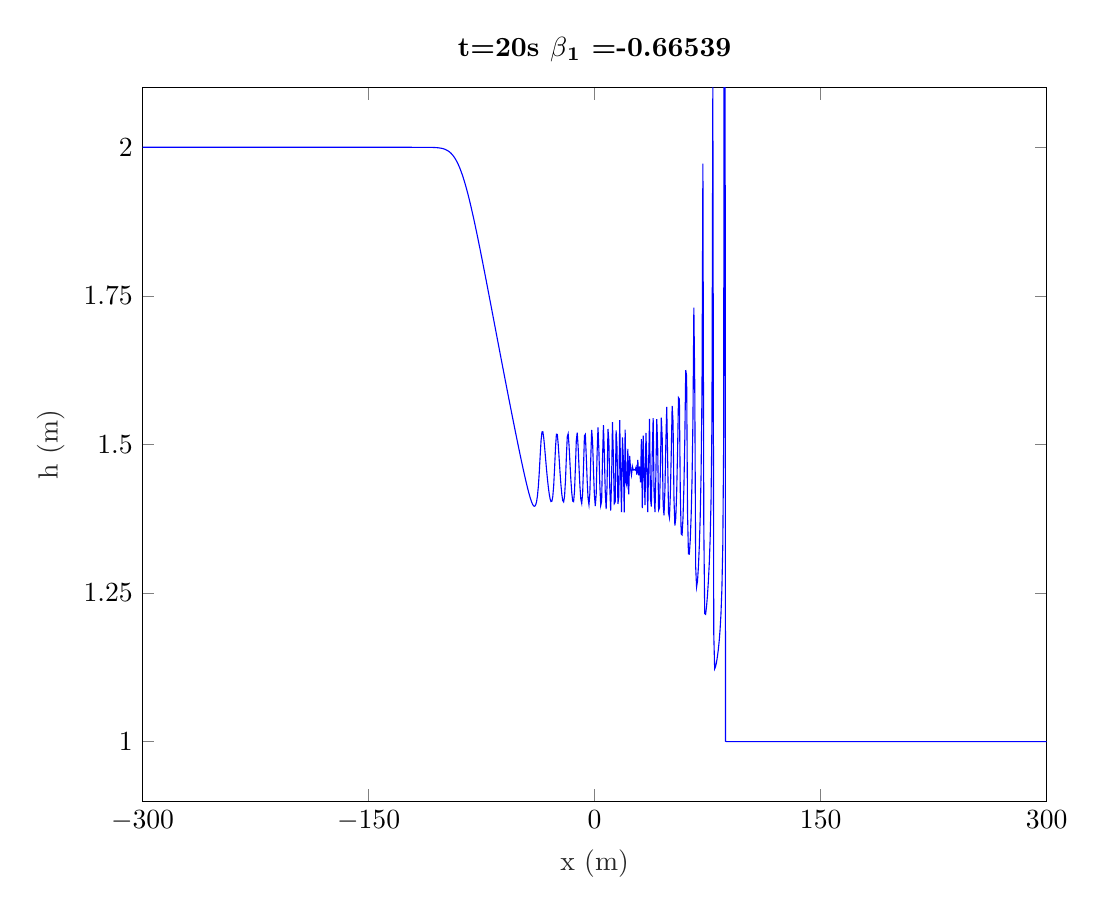
\begin{tikzpicture}

\begin{axis}[%
width=4.521in,
height=3.566in,
at={(0.758in,0.481in)},
scale only axis,
xmin=-300,
xmax=300,
xtick={-300, -150,    0,  150,  300},
xlabel style={font=\color{white!15!black}},
xlabel={x (m)},
ymin=0.9,
ymax=2.1,
ytick={   1, 1.25,  1.5, 1.75,    2},
ylabel style={font=\color{white!15!black}},
ylabel={h (m)},
axis background/.style={fill=white},
title style={font=\bfseries},
title={$\text{t=20s   }\beta{}_\text{1}\text{ =-0.66539}$}
]
\addplot [color=blue, forget plot]
  table[row sep=crcr]{%
-300.18000900045	2\\
-299.57997899895	2\\
-298.97994899745	2\\
-298.37991899595	2\\
-297.77988899445	2\\
-297.17985899295	2\\
-296.57982899145	2\\
-295.979798989949	2\\
-295.379768988449	2\\
-294.779738986949	2\\
-294.179708985449	2\\
-293.579678983949	2\\
-292.979648982449	2\\
-292.379618980949	2\\
-291.779588979449	2\\
-291.179558977949	2\\
-290.579528976449	2\\
-289.979498974949	2\\
-289.379468973449	2\\
-288.779438971949	2\\
-288.179408970449	2\\
-287.579378968948	2\\
-286.979348967448	2\\
-286.379318965948	2\\
-285.779288964448	2\\
-285.179258962948	2\\
-284.579228961448	2\\
-283.979198959948	2\\
-283.379168958448	2\\
-282.779138956948	2\\
-282.179108955448	2\\
-281.579078953948	2\\
-280.979048952448	2\\
-280.379018950948	2\\
-279.778988949447	2\\
-279.178958947947	2\\
-278.578928946447	2\\
-277.978898944947	2\\
-277.378868943447	2\\
-276.778838941947	2\\
-276.178808940447	2\\
-275.578778938947	2\\
-274.978748937447	2\\
-274.378718935947	2\\
-273.778688934447	2\\
-273.178658932947	2\\
-272.578628931447	2\\
-271.978598929946	2\\
-271.378568928446	2\\
-270.778538926946	2\\
-270.178508925446	2\\
-269.578478923946	2\\
-268.978448922446	2\\
-268.378418920946	2\\
-267.778388919446	2\\
-267.178358917946	2\\
-266.578328916446	2\\
-265.978298914946	2\\
-265.378268913446	2\\
-264.778238911946	2\\
-264.178208910446	2\\
-263.578178908945	2\\
-262.978148907445	2\\
-262.378118905945	2\\
-261.778088904445	2\\
-261.178058902945	2\\
-260.578028901445	2\\
-259.977998899945	2\\
-259.377968898445	2\\
-258.777938896945	2\\
-258.177908895445	2\\
-257.577878893945	2\\
-256.977848892445	2\\
-256.377818890945	2\\
-255.777788889444	2\\
-255.177758887944	2\\
-254.577728886444	2\\
-253.977698884944	2\\
-253.377668883444	2\\
-252.777638881944	2\\
-252.177608880444	2\\
-251.577578878944	2\\
-250.977548877444	2\\
-250.377518875944	2\\
-249.777488874444	2\\
-249.177458872944	2\\
-248.577428871444	2\\
-247.977398869943	2\\
-247.377368868443	2\\
-246.777338866943	2\\
-246.177308865443	2\\
-245.577278863943	2\\
-244.977248862443	2\\
-244.377218860943	2\\
-243.777188859443	2\\
-243.177158857943	2\\
-242.577128856443	2\\
-241.977098854943	2\\
-241.377068853443	2\\
-240.777038851943	2\\
-240.177008850443	2\\
-239.576978848942	2\\
-238.976948847442	2\\
-238.376918845942	2\\
-237.776888844442	2\\
-237.176858842942	2\\
-236.576828841442	2\\
-235.976798839942	2\\
-235.376768838442	2\\
-234.776738836942	2\\
-234.176708835442	2\\
-233.576678833942	2\\
-232.976648832442	2\\
-232.376618830942	2\\
-231.776588829441	2\\
-231.176558827941	2\\
-230.576528826441	2\\
-229.976498824941	2\\
-229.376468823441	2\\
-228.776438821941	2\\
-228.176408820441	2\\
-227.576378818941	2\\
-226.976348817441	2\\
-226.376318815941	2\\
-225.776288814441	2\\
-225.176258812941	2\\
-224.576228811441	2\\
-223.976198809941	2\\
-223.37616880844	2\\
-222.77613880694	2\\
-222.17610880544	2\\
-221.57607880394	2\\
-220.97604880244	2\\
-220.37601880094	2\\
-219.77598879944	2\\
-219.17595879794	2\\
-218.57592879644	2\\
-217.97589879494	2\\
-217.37586879344	2\\
-216.77583879194	2\\
-216.17580879044	2\\
-215.575778788939	2\\
-214.975748787439	2\\
-214.375718785939	2\\
-213.775688784439	2\\
-213.175658782939	2\\
-212.575628781439	2\\
-211.975598779939	2\\
-211.375568778439	2\\
-210.775538776939	2\\
-210.175508775439	2\\
-209.575478773939	2\\
-208.975448772439	2\\
-208.375418770939	2\\
-207.775388769438	2\\
-207.175358767938	2\\
-206.575328766438	2\\
-205.975298764938	2\\
-205.375268763438	2\\
-204.775238761938	2\\
-204.175208760438	2\\
-203.575178758938	2\\
-202.975148757438	2\\
-202.375118755938	2\\
-201.775088754438	2\\
-201.175058752938	2\\
-200.575028751438	2\\
-199.974998749937	2\\
-199.374968748437	2\\
-198.774938746937	2\\
-198.174908745437	2\\
-197.574878743937	2\\
-196.974848742437	2\\
-196.374818740937	2\\
-195.774788739437	2\\
-195.174758737937	2\\
-194.574728736437	2\\
-193.974698734937	2\\
-193.374668733437	2\\
-192.774638731937	2\\
-192.174608730437	2\\
-191.574578728936	2\\
-190.974548727436	2\\
-190.374518725936	2\\
-189.774488724436	2\\
-189.174458722936	2\\
-188.574428721436	2\\
-187.974398719936	2\\
-187.374368718436	2\\
-186.774338716936	2\\
-186.174308715436	2\\
-185.574278713936	2\\
-184.974248712436	2\\
-184.374218710936	2\\
-183.774188709435	2\\
-183.174158707935	2\\
-182.574128706435	2\\
-181.974098704935	2\\
-181.374068703435	2\\
-180.774038701935	2\\
-180.174008700435	2\\
-179.573978698935	2\\
-178.973948697435	2\\
-178.373918695935	2\\
-177.773888694435	2\\
-177.173858692935	2\\
-176.573828691435	2\\
-175.973798689934	2\\
-175.373768688434	2\\
-174.773738686934	2\\
-174.173708685434	2\\
-173.573678683934	2\\
-172.973648682434	2\\
-172.373618680934	2\\
-171.773588679434	2\\
-171.173558677934	2\\
-170.573528676434	2\\
-169.973498674934	2\\
-169.373468673434	2\\
-168.773438671934	2\\
-168.173408670434	2\\
-167.573378668933	2\\
-166.973348667433	2\\
-166.373318665933	2\\
-165.773288664433	2\\
-165.173258662933	2\\
-164.573228661433	2\\
-163.973198659933	2\\
-163.373168658433	2\\
-162.773138656933	2\\
-162.173108655433	2\\
-161.573078653933	2\\
-160.973048652433	2\\
-160.373018650933	2\\
-159.772988649432	2\\
-159.172958647932	2\\
-158.572928646432	2\\
-157.972898644932	2\\
-157.372868643432	2\\
-156.772838641932	2\\
-156.172808640432	2\\
-155.572778638932	2\\
-154.972748637432	1.99999999999998\\
-154.372718635932	1.99999999999997\\
-153.772688634432	1.99999999999995\\
-153.172658632932	1.99999999999991\\
-152.572628631432	1.99999999999987\\
-151.972598629931	1.99999999999981\\
-151.372568628431	1.99999999999973\\
-150.772538626931	1.99999999999961\\
-150.172508625431	1.99999999999946\\
-149.572478623931	1.99999999999925\\
-148.972448622431	1.99999999999896\\
-148.372418620931	1.99999999999856\\
-147.772388619431	1.99999999999802\\
-147.172358617931	1.99999999999728\\
-146.572328616431	1.99999999999625\\
-145.972298614931	1.99999999999485\\
-145.372268613431	1.99999999999294\\
-144.772238611931	1.99999999999033\\
-144.172208610431	1.99999999998676\\
-143.57217860893	1.99999999998192\\
-142.97214860743	1.99999999997531\\
-142.37211860593	1.99999999996634\\
-141.77208860443	1.99999999995415\\
-141.17205860293	1.99999999993762\\
-140.57202860143	1.99999999991521\\
-139.97199859993	1.99999999988489\\
-139.37196859843	1.99999999984387\\
-138.77193859693	1.99999999978848\\
-138.17190859543	1.99999999971375\\
-137.57187859393	1.99999999961304\\
-136.97184859243	1.99999999947747\\
-136.37181859093	1.99999999929522\\
-135.771788589429	1.99999999905047\\
-135.171758587929	1.99999999872222\\
-134.571728586429	1.9999999982825\\
-133.971698584929	1.99999999769419\\
-133.371668583429	1.99999999690808\\
-132.771638581929	1.99999999585899\\
-132.171608580429	1.99999999446078\\
-131.571578578929	1.99999999259971\\
-130.971548577429	1.99999999012585\\
-130.371518575929	1.99999998684187\\
-129.771488574429	1.99999998248846\\
-129.171458572929	1.99999997672538\\
-128.571428571429	1.99999996910695\\
-127.971398569929	1.9999999590503\\
-127.371368568428	1.9999999457944\\
-126.771338566928	1.99999992834732\\
-126.171308565428	1.99999990541836\\
-125.571278563928	1.99999987533107\\
-124.971248562428	1.99999983591176\\
-124.371218560928	1.99999978434727\\
-123.771188559428	1.99999971700355\\
-123.171158557928	1.99999962919506\\
-122.571128556428	1.99999951489225\\
-121.971098554928	1.99999936635137\\
-121.371068553428	1.99999917364729\\
-120.771038551928	1.99999892408528\\
-120.171008550428	1.99999860146252\\
-119.570978548927	1.99999818514342\\
-118.970948547427	1.99999764890517\\
-118.370918545927	1.99999695950062\\
-117.770888544427	1.99999607487487\\
-117.170858542927	1.99999494195896\\
-116.570828541427	1.99999349394972\\
-115.970798539927	1.99999164696745\\
-115.370768538427	1.99998929596389\\
-114.770738536927	1.99998630973143\\
-114.170708535427	1.99998252484005\\
-113.570678533927	1.9999777383024\\
-112.970648532427	1.99997169873915\\
-112.370618530927	1.99996409578744\\
-111.770588529426	1.99995454746587\\
-111.170558527926	1.99994258518107\\
-110.570528526426	1.99992763603602\\
-109.970498524926	1.99990900208094\\
-109.370468523426	1.99988583613805\\
-108.770438521926	1.99985711383449\\
-108.170408520426	1.99982160150055\\
-107.570378518926	1.99977781963696\\
-106.970348517426	1.99972400173367\\
-106.370318515926	1.99965804834084\\
-105.770288514426	1.99957747645781\\
-105.170258512926	1.99947936452577\\
-104.570228511426	1.99936029359148\\
-103.970198509925	1.9992162855555\\
-103.370168508425	1.9990427398304\\
-102.770138506925	1.99883437020604\\
-102.170108505425	1.99858514423659\\
-101.570078503925	1.99828822800589\\
-100.970048502425	1.99793593965763\\
-100.370018500925	1.99751971555082\\
-99.769988499425	1.99703009325862\\
-99.1699584979249	1.99645671580481\\
-98.5699284964248	1.99578836145427\\
-97.9698984949247	1.99501300297462\\
-97.3698684934247	1.9941178995099\\
-96.7698384919246	1.99308972302639\\
-96.1698084904245	1.99191471971072\\
-95.5697784889244	1.99057890477931\\
-94.9697484874244	1.98906828700143\\
-94.3697184859243	1.98736911700671\\
-93.7696884844242	1.98546815133933\\
-93.1696584829241	1.98335292245527\\
-92.5696284814241	1.98101200364716\\
-91.969598479924	1.97843525739681\\
-91.3695684784239	1.97561405600306\\
-90.7695384769239	1.97254146452975\\
-90.1695084754238	1.96921237808331\\
-89.5694784739237	1.96562360799162\\
-88.9694484724236	1.96177391437592\\
-88.3694184709235	1.95766398561192\\
-87.7693884694235	1.95329636799308\\
-87.1693584679234	1.9486753513051\\
-86.5693284664233	1.94380681782708\\
-85.9692984649232	1.93869806340119\\
-85.3692684634232	1.93335759965093\\
-84.7692384619231	1.92779494623591\\
-84.169208460423	1.92202042132207\\
-83.5691784589229	1.9160449373586\\
-82.9691484574229	1.90987980793662\\
-82.3691184559228	1.9035365700965\\
-81.7690884544227	1.89702682506925\\
-81.1690584529227	1.89036209916846\\
-80.5690284514226	1.88355372545211\\
-79.9689984499225	1.87661274587808\\
-79.3689684484224	1.86954983298978\\
-78.7689384469223	1.86237522968014\\
-78.1689084454223	1.85509870527021\\
-77.5688784439222	1.8477295259766\\
-76.9688484424221	1.84027643779806\\
-76.368818440922	1.83274765989878\\
-75.768788439422	1.82515088667578\\
-75.1687584379219	1.81749329684924\\
-74.5687284364218	1.80978156808919\\
-73.9686984349217	1.80202189587471\\
-73.3686684334217	1.79422001546332\\
-72.7686384319216	1.78638122602129\\
-72.1686084304215	1.77851041612461\\
-71.5685784289215	1.77061208998474\\
-70.9685484274214	1.76269039388012\\
-70.3685184259213	1.7547491423849\\
-69.7684884244212	1.74679184408215\\
-69.1684584229211	1.73882172652829\\
-68.5684284214211	1.7308417603047\\
-67.968398419921	1.72285468204806\\
-67.3683684184209	1.71486301639863\\
-66.7683384169208	1.70686909684478\\
-66.1683084154208	1.69887508547418\\
-65.5682784139207	1.69088299166922\\
-64.9682484124206	1.6828946898071\\
-64.3682184109205	1.67491193604452\\
-63.7681884094205	1.6669363842843\\
-63.1681584079204	1.65896960143728\\
-62.5681284064203	1.65101308210841\\
-61.9680984049203	1.64306826285191\\
-61.3680684034202	1.63513653615756\\
-60.7680384019201	1.62721926434951\\
-60.16800840042	1.61931779360238\\
-59.5679783989199	1.61143346830654\\
-58.9679483974199	1.603567646049\\
-58.3679183959198	1.59572171351882\\
-57.7678883944197	1.58789710369952\\
-57.1678583929196	1.58009531477916\\
-56.5678283914196	1.57231793129591\\
-55.9677983899195	1.56456664814797\\
-55.3677683884194	1.55684329824131\\
-54.7677383869193	1.54914988473431\\
-54.1677083854193	1.54148861908207\\
-53.5676783839192	1.53386196640168\\
-52.9676483824191	1.52627270010044\\
-52.3676183809191	1.51872396826906\\
-51.767588379419	1.51121937509152\\
-51.1675583779189	1.50376308153729\\
-50.5675283764188	1.49635993098399\\
-49.9674983749187	1.48901560732199\\
-49.3674683734187	1.48173683574015\\
-48.7674383719186	1.47453164011514\\
-48.1674083704185	1.46740967622183\\
-47.5673783689184	1.46038266760648\\
-46.9673483674184	1.4534649820802\\
-46.3673183659183	1.44667440321752\\
-45.7672883644182	1.44003317585744\\
-45.1672583629181	1.43356944201618\\
-44.5672283614181	1.42731924131359\\
-43.967198359918	1.421329340264\\
-43.3671683584179	1.4156612978434\\
-42.7671383569178	1.41039740402218\\
-42.1671083554178	1.40564949764328\\
-41.5670783539177	1.40157226376366\\
-40.9670483524176	1.39838353960062\\
-40.3670183509175	1.39639548170783\\
-39.7669883494175	1.39606246545715\\
-39.1669583479174	1.39804909017868\\
-38.5669283464173	1.40331939959109\\
-37.9668983449172	1.41319535775176\\
-37.3668683434172	1.42920171953841\\
-36.7668383419171	1.45219152209228\\
-36.166808340417	1.48015365961418\\
-35.5667783389169	1.50609970610429\\
-34.9667483374168	1.52104615130345\\
-34.3667183359168	1.52148294336858\\
-33.7666883344167	1.51087122720023\\
-33.1666583329167	1.49461163431472\\
-32.5666283314166	1.47662922683657\\
-31.9665983299165	1.4590642127174\\
-31.3665683284164	1.44296485435423\\
-30.7665383269164	1.42888718803003\\
-30.1665083254163	1.41726378595999\\
-29.5664783239162	1.40864214963671\\
-28.9664483224161	1.40389340210967\\
-28.3664183209161	1.40445586082853\\
-27.766388319416	1.41256318900731\\
-27.1663583179159	1.43101314302169\\
-26.5663283164158	1.46081336185665\\
-25.9662983149157	1.4950452078113\\
-25.3662683134157	1.5172162138687\\
-24.7662383119156	1.51700666158101\\
-24.1662083104155	1.50004924827451\\
-23.5661783089154	1.47652459705629\\
-22.9661483074154	1.45289331756061\\
-22.3661183059153	1.43217492097902\\
-21.7660883044152	1.41592679120209\\
-21.1660583029151	1.40558632490717\\
-20.5660283014151	1.40336444264405\\
-19.965998299915	1.41289816366879\\
-19.3659682984149	1.43855163049373\\
-18.7659382969148	1.47861059343076\\
-18.1659082954148	1.51300551201322\\
-17.5658782939147	1.51802276489843\\
-16.9658482924146	1.49751080870748\\
-16.3658182909145	1.46815146674136\\
-15.7657882894144	1.44024483810967\\
-15.1657582879144	1.41821374543114\\
-14.5657282864143	1.40479494909984\\
-13.9656982849143	1.4037039282739\\
-13.3656682834142	1.42095180145102\\
-12.7656382819141	1.46084883529825\\
-12.165608280414	1.50669898800621\\
-11.565578278914	1.51996199139564\\
-10.9655482774139	1.49675448179546\\
-10.3655182759138	1.46146768150313\\
-9.76548827441371	1.42962465140307\\
-9.16545827291367	1.40769472224305\\
-8.56542827141357	1.40085794047134\\
-7.96539826991352	1.41730921664887\\
-7.36536826841342	1.4639205225583\\
-6.76533826691332	1.51466349376672\\
-6.16530826541327	1.51703380697022\\
-5.56527826391317	1.48069117816436\\
-4.96524826241313	1.43969559896712\\
-4.36521826091303	1.40962358463362\\
-3.76518825941298	1.39866584370711\\
-3.16515825791288	1.41834875944655\\
-2.56512825641283	1.47649580090714\\
-1.96509825491273	1.52453217905179\\
-1.36506825341269	1.50476274044684\\
-0.765038251912586	1.45569161946689\\
-0.165008250412541	1.41460361219127\\
0.435021751087561	1.39624361540005\\
1.03505175258761	1.41652478325879\\
1.63508175408771	1.48574237307273\\
2.23511175558775	1.52883478837645\\
2.83514175708785	1.48916655738449\\
3.43517175858796	1.4324220493498\\
4.035201760088	1.39728242909289\\
4.6352317615881	1.4044806767827\\
5.23526176308815	1.47608940495773\\
5.83529176458825	1.53236181756437\\
6.43532176608829	1.48429982546888\\
7.03535176758839	1.42027272517448\\
7.63538176908844	1.39110402251876\\
8.23541177058854	1.4302654816311\\
8.83544177208859	1.52598304023489\\
9.43547177358869	1.50575908163208\\
10.0355017750887	1.4278197932732\\
10.6355317765888	1.38890505253643\\
11.2355617780889	1.43832793314859\\
11.835591779589	1.53762098404067\\
12.435621781089	1.47976778222708\\
13.0356517825891	1.40045595785245\\
13.6356817840892	1.40322591542182\\
14.2357117855893	1.52351758076104\\
14.8357417870894	1.49573542963326\\
15.4357717885894	1.39993145510729\\
16.0358017900895	1.41198000545111\\
16.6358317915896	1.5408650849976\\
17.2358617930897	1.45331415518602\\
17.8358917945897	1.38629733470177\\
18.4359217960898	1.51180750590596\\
19.0359517975899	1.47699425883363\\
19.63598179909	1.38585978695387\\
20.23601180059	1.52479705913696\\
20.8360418020901	1.43575113319475\\
21.4360718035902	1.43012417680538\\
22.0361018050903	1.49251854288509\\
22.6361318065904	1.4160086349335\\
23.2361618080904	1.48091235955574\\
23.8361918095905	1.45873645912597\\
24.4362218110905	1.44872117560191\\
25.0362518125906	1.46315254068791\\
25.6362818140907	1.45695461617351\\
26.2363118155908	1.45755480038834\\
26.8363418170908	1.45680126107533\\
27.4363718185909	1.46136870947753\\
28.036401820091	1.44912852353657\\
28.6364318215911	1.47423270639072\\
29.2364618230911	1.44803970124373\\
29.8364918245912	1.46286602363155\\
30.4365218260913	1.43626980483965\\
31.0365518275914	1.50914986321485\\
31.6365818290914	1.39273375871496\\
32.2366118305915	1.51467773473557\\
32.8366418320916	1.44744131868776\\
33.4366718335917	1.39790260300464\\
34.0367018350918	1.51955587641191\\
34.6367318365918	1.46905012196139\\
35.2367618380919	1.38608818631036\\
35.836791839592	1.46978940473976\\
36.4368218410921	1.54293980793083\\
37.0368518425921	1.40874727058557\\
37.6368818440922	1.39558417609282\\
38.2369118455923	1.48639861225395\\
38.8369418470924	1.54438403585309\\
39.4369718485924	1.4177879562827\\
40.0370018500925	1.38606564131984\\
40.6370318515926	1.44962008460146\\
41.2370618530927	1.54251866405343\\
41.8370918545928	1.49433516151437\\
42.4371218560928	1.38964046457827\\
43.0371518575929	1.39336824185027\\
43.6371818590929	1.45942219501669\\
44.237211860593	1.54522482897806\\
44.8372418620931	1.51073454919109\\
45.4372718635932	1.39852703571124\\
46.0373018650932	1.38092364605715\\
46.6373318665933	1.42368305784665\\
47.2373618680934	1.50161332569055\\
47.8373918695935	1.56341302675265\\
48.4374218710935	1.47759296647351\\
49.0374518725936	1.38472020040981\\
49.6374818740937	1.37686991231872\\
50.2375118755938	1.41528072939716\\
50.8375418770938	1.48476520541351\\
51.4375718785939	1.56508140062899\\
52.037601880094	1.53799861280182\\
52.6376318815941	1.40915543743726\\
53.2376618830942	1.3634658436639\\
53.8376918845942	1.37578930889314\\
54.4377218860943	1.4191701696095\\
55.0377518875944	1.48941274471326\\
55.6377818890945	1.5788553568603\\
56.2378118905945	1.57657252156467\\
56.8378418920946	1.41902457426208\\
57.4378718935947	1.34950862359233\\
58.0379018950948	1.34794558343874\\
58.6379318965948	1.37647563040886\\
59.2379618980949	1.42802975614648\\
59.837991899595	1.50893568763638\\
60.4380219010951	1.62517506428562\\
61.0380519025952	1.61534782994243\\
61.6380819040952	1.38563001661885\\
62.2381119055953	1.31588283158221\\
62.8381419070953	1.31552122753079\\
63.4381719085955	1.33921426929495\\
64.0382019100955	1.37946264631143\\
64.6382319115956	1.44098328201846\\
65.2382619130956	1.54289209080662\\
65.8382919145957	1.73003695029011\\
66.4383219160958	1.60000551839763\\
67.0383519175959	1.29434865441783\\
67.6383819190959	1.26022215821469\\
68.238411920596	1.2695543184984\\
68.8384419220961	1.29313608665996\\
69.4384719235962	1.32760150599234\\
70.0385019250962	1.37634054931193\\
70.6385319265963	1.45097749168563\\
71.2385619280964	1.59067163686541\\
71.8385919295965	1.97272013113284\\
72.4386219310966	1.36195442050509\\
73.0386519325966	1.21541900947635\\
73.6386819340967	1.21415765571236\\
74.2387119355968	1.22701280380471\\
74.8387419370969	1.24528511252114\\
75.4387719385969	1.2684805992846\\
76.038801940097	1.2985045572228\\
76.6388319415971	1.34012429884733\\
77.2388619430972	1.40543938220156\\
77.8388919445972	1.53650140397437\\
78.4389219460973	2.1108829023394\\
79.0389519475974	1.18246257510866\\
79.6389819490975	1.12244469187345\\
80.2390119505975	1.12593285439786\\
80.8390419520976	1.13328203270357\\
81.4390719535977	1.14264959441957\\
82.0391019550977	1.15428521596594\\
82.6391319565979	1.16903607274565\\
83.2391619580979	1.18846270894011\\
83.839191959598	1.21555648529546\\
84.439221961098	1.25682542323288\\
85.0392519625981	1.32891802240021\\
85.6392819640982	1.51160739815568\\
86.2393119655983	3.71389524327639\\
86.8393419670983	1.00082169349943\\
87.4393719685984	1.00004067502193\\
88.0394019700985	1.00000667871753\\
88.6394319715986	1.0000017227266\\
89.2394619730986	1.00000055844759\\
89.8394919745987	1.00000020655971\\
90.4395219760988	1.00000008298411\\
91.0395519775989	1.00000003521692\\
91.639581979099	1.00000001552397\\
92.239611980599	1.00000000703198\\
92.8396419820991	1.00000000324984\\
93.4396719835992	1.00000000152476\\
94.0397019850993	1.00000000072372\\
94.6397319865993	1.00000000034661\\
95.2397619880994	1.00000000016718\\
95.8397919895995	1.00000000008109\\
96.4398219910996	1.00000000003951\\
97.0398519925996	1.00000000001932\\
97.6398819940997	1.00000000000947\\
98.2399119955998	1.00000000000465\\
98.8399419970999	1.00000000000229\\
99.4399719985999	1.00000000000112\\
100.0400020001	1.00000000000055\\
100.6400320016	1.00000000000027\\
101.2400620031	1.00000000000013\\
101.8400920046	1.00000000000006\\
102.4401220061	1.00000000000002\\
103.0401520076	1\\
103.6401820091	1\\
104.240212010601	1\\
104.840242012101	1\\
105.440272013601	1\\
106.040302015101	1\\
106.640332016601	1\\
107.240362018101	1\\
107.840392019601	1\\
108.440422021101	1\\
109.040452022601	1\\
109.640482024101	1\\
110.240512025601	1\\
110.840542027101	1\\
111.440572028601	1\\
112.040602030102	1\\
112.640632031602	1\\
113.240662033102	1\\
113.840692034602	1\\
114.440722036102	1\\
115.040752037602	1\\
115.640782039102	1\\
116.240812040602	1\\
116.840842042102	1\\
117.440872043602	1\\
118.040902045102	1\\
118.640932046602	1\\
119.240962048102	1\\
119.840992049603	1\\
120.441022051103	1\\
121.041052052603	1\\
121.641082054103	1\\
122.241112055603	1\\
122.841142057103	1\\
123.441172058603	1\\
124.041202060103	1\\
124.641232061603	1\\
125.241262063103	1\\
125.841292064603	1\\
126.441322066103	1\\
127.041352067603	1\\
127.641382069103	1\\
128.241412070604	1\\
128.841442072104	1\\
129.441472073604	1\\
130.041502075104	1\\
130.641532076604	1\\
131.241562078104	1\\
131.841592079604	1\\
132.441622081104	1\\
133.041652082604	1\\
133.641682084104	1\\
134.241712085604	1\\
134.841742087104	1\\
135.441772088604	1\\
136.041802090105	1\\
136.641832091605	1\\
137.241862093105	1\\
137.841892094605	1\\
138.441922096105	1\\
139.041952097605	1\\
139.641982099105	1\\
140.242012100605	1\\
140.842042102105	1\\
141.442072103605	1\\
142.042102105105	1\\
142.642132106605	1\\
143.242162108105	1\\
143.842192109605	1\\
144.442222111106	1\\
145.042252112606	1\\
145.642282114106	1\\
146.242312115606	1\\
146.842342117106	1\\
147.442372118606	1\\
148.042402120106	1\\
148.642432121606	1\\
149.242462123106	1\\
149.842492124606	1\\
150.442522126106	1\\
151.042552127606	1\\
151.642582129106	1\\
152.242612130607	1\\
152.842642132107	1\\
153.442672133607	1\\
154.042702135107	1\\
154.642732136607	1\\
155.242762138107	1\\
155.842792139607	1\\
156.442822141107	1\\
157.042852142607	1\\
157.642882144107	1\\
158.242912145607	1\\
158.842942147107	1\\
159.442972148607	1\\
160.043002150107	1\\
160.643032151608	1\\
161.243062153108	1\\
161.843092154608	1\\
162.443122156108	1\\
163.043152157608	1\\
163.643182159108	1\\
164.243212160608	1\\
164.843242162108	1\\
165.443272163608	1\\
166.043302165108	1\\
166.643332166608	1\\
167.243362168108	1\\
167.843392169608	1\\
168.443422171109	1\\
169.043452172609	1\\
169.643482174109	1\\
170.243512175609	1\\
170.843542177109	1\\
171.443572178609	1\\
172.043602180109	1\\
172.643632181609	1\\
173.243662183109	1\\
173.843692184609	1\\
174.443722186109	1\\
175.043752187609	1\\
175.643782189109	1\\
176.24381219061	1\\
176.84384219211	1\\
177.44387219361	1\\
178.04390219511	1\\
178.64393219661	1\\
179.24396219811	1\\
179.84399219961	1\\
180.44402220111	1\\
181.04405220261	1\\
181.64408220411	1\\
182.24411220561	1\\
182.84414220711	1\\
183.44417220861	1\\
184.04420221011	1\\
184.644232211611	1\\
185.244262213111	1\\
185.844292214611	1\\
186.444322216111	1\\
187.044352217611	1\\
187.644382219111	1\\
188.244412220611	1\\
188.844442222111	1\\
189.444472223611	1\\
190.044502225111	1\\
190.644532226611	1\\
191.244562228111	1\\
191.844592229611	1\\
192.444622231112	1\\
193.044652232612	1\\
193.644682234112	1\\
194.244712235612	1\\
194.844742237112	1\\
195.444772238612	1\\
196.044802240112	1\\
196.644832241612	1\\
197.244862243112	1\\
197.844892244612	1\\
198.444922246112	1\\
199.044952247612	1\\
199.644982249112	1\\
200.245012250613	1\\
200.845042252113	1\\
201.445072253613	1\\
202.045102255113	1\\
202.645132256613	1\\
203.245162258113	1\\
203.845192259613	1\\
204.445222261113	1\\
205.045252262613	1\\
205.645282264113	1\\
206.245312265613	1\\
206.845342267113	1\\
207.445372268613	1\\
208.045402270114	1\\
208.645432271614	1\\
209.245462273114	1\\
209.845492274614	1\\
210.445522276114	1\\
211.045552277614	1\\
211.645582279114	1\\
212.245612280614	1\\
212.845642282114	1\\
213.445672283614	1\\
214.045702285114	1\\
214.645732286614	1\\
215.245762288114	1\\
215.845792289614	1\\
216.445822291115	1\\
217.045852292615	1\\
217.645882294115	1\\
218.245912295615	1\\
218.845942297115	1\\
219.445972298615	1\\
220.046002300115	1\\
220.646032301615	1\\
221.246062303115	1\\
221.846092304615	1\\
222.446122306115	1\\
223.046152307615	1\\
223.646182309115	1\\
224.246212310616	1\\
224.846242312116	1\\
225.446272313616	1\\
226.046302315116	1\\
226.646332316616	1\\
227.246362318116	1\\
227.846392319616	1\\
228.446422321116	1\\
229.046452322616	1\\
229.646482324116	1\\
230.246512325616	1\\
230.846542327116	1\\
231.446572328616	1\\
232.046602330116	1\\
232.646632331617	1\\
233.246662333117	1\\
233.846692334617	1\\
234.446722336117	1\\
235.046752337617	1\\
235.646782339117	1\\
236.246812340617	1\\
236.846842342117	1\\
237.446872343617	1\\
238.046902345117	1\\
238.646932346617	1\\
239.246962348117	1\\
239.846992349617	1\\
240.447022351118	1\\
241.047052352618	1\\
241.647082354118	1\\
242.247112355618	1\\
242.847142357118	1\\
243.447172358618	1\\
244.047202360118	1\\
244.647232361618	1\\
245.247262363118	1\\
245.847292364618	1\\
246.447322366118	1\\
247.047352367618	1\\
247.647382369118	1\\
248.247412370619	1\\
248.847442372119	1\\
249.447472373619	1\\
250.047502375119	1\\
250.647532376619	1\\
251.247562378119	1\\
251.847592379619	1\\
252.447622381119	1\\
253.047652382619	1\\
253.647682384119	1\\
254.247712385619	1\\
254.847742387119	1\\
255.447772388619	1\\
256.04780239012	1\\
256.64783239162	1\\
257.24786239312	1\\
257.84789239462	1\\
258.44792239612	1\\
259.04795239762	1\\
259.64798239912	1\\
260.24801240062	1\\
260.84804240212	1\\
261.44807240362	1\\
262.04810240512	1\\
262.64813240662	1\\
263.24816240812	1\\
263.84819240962	1\\
264.448222411121	1\\
265.048252412621	1\\
265.648282414121	1\\
266.248312415621	1\\
266.848342417121	1\\
267.448372418621	1\\
268.048402420121	1\\
268.648432421621	1\\
269.248462423121	1\\
269.848492424621	1\\
270.448522426121	1\\
271.048552427621	1\\
271.648582429121	1\\
272.248612430622	1\\
272.848642432122	1\\
273.448672433622	1\\
274.048702435122	1\\
274.648732436622	1\\
275.248762438122	1\\
275.848792439622	1\\
276.448822441122	1\\
277.048852442622	1\\
277.648882444122	1\\
278.248912445622	1\\
278.848942447122	1\\
279.448972448622	1\\
280.049002450123	1\\
280.649032451623	1\\
281.249062453123	1\\
281.849092454623	1\\
282.449122456123	1\\
283.049152457623	1\\
283.649182459123	1\\
284.249212460623	1\\
284.849242462123	1\\
285.449272463623	1\\
286.049302465123	1\\
286.649332466623	1\\
287.249362468123	1\\
287.849392469623	1\\
288.449422471124	1\\
289.049452472624	1\\
289.649482474124	1\\
290.249512475624	1\\
290.849542477124	1\\
291.449572478624	1\\
292.049602480124	1\\
292.649632481624	1\\
293.249662483124	1\\
293.849692484624	1\\
294.449722486124	1\\
295.049752487624	1\\
295.649782489125	1\\
296.249812490625	1\\
296.849842492125	1\\
297.449872493625	1\\
298.049902495125	1\\
298.649932496625	1\\
299.249962498125	1\\
299.849992499625	1\\
};
\end{axis}
\end{tikzpicture}%
		\caption{$t=20s$}
	\end{subfigure}
	\begin{subfigure}{0.49\textwidth}
		\centering
		% This file was created by matlab2tikz.
%
%The latest updates can be retrieved from
%  http://www.mathworks.com/matlabcentral/fileexchange/22022-matlab2tikz-matlab2tikz
%where you can also make suggestions and rate matlab2tikz.
%
\begin{tikzpicture}

\begin{axis}[%
width=4.521in,
height=3.566in,
at={(0.758in,0.481in)},
scale only axis,
xmin=-300,
xmax=300,
xtick={-300, -150,    0,  150,  300},
xlabel style={font=\color{white!15!black}},
xlabel={x (m)},
ymin=0.9,
ymax=2.1,
ytick={   1, 1.25,  1.5, 1.75,    2},
ylabel style={font=\color{white!15!black}},
ylabel={h (m)},
axis background/.style={fill=white},
title style={font=\bfseries},
title={$\text{t=30s   }\beta{}_\text{1}\text{ =-0.66667}$}
]
\addplot [color=blue, forget plot]
  table[row sep=crcr]{%
-300.18000900045	2\\
-299.57997899895	2\\
-298.97994899745	2\\
-298.37991899595	2\\
-297.77988899445	2\\
-297.17985899295	2\\
-296.57982899145	2\\
-295.979798989949	2\\
-295.379768988449	2\\
-294.779738986949	2\\
-294.179708985449	2\\
-293.579678983949	2\\
-292.979648982449	2\\
-292.379618980949	2\\
-291.779588979449	2\\
-291.179558977949	2\\
-290.579528976449	2\\
-289.979498974949	2\\
-289.379468973449	2\\
-288.779438971949	2\\
-288.179408970449	2\\
-287.579378968948	2\\
-286.979348967448	2\\
-286.379318965948	2\\
-285.779288964448	2\\
-285.179258962948	2\\
-284.579228961448	2\\
-283.979198959948	2\\
-283.379168958448	2\\
-282.779138956948	2\\
-282.179108955448	2\\
-281.579078953948	2\\
-280.979048952448	2\\
-280.379018950948	2\\
-279.778988949447	2\\
-279.178958947947	2\\
-278.578928946447	2\\
-277.978898944947	2\\
-277.378868943447	2\\
-276.778838941947	2\\
-276.178808940447	2\\
-275.578778938947	2\\
-274.978748937447	2\\
-274.378718935947	2\\
-273.778688934447	2\\
-273.178658932947	2\\
-272.578628931447	2\\
-271.978598929946	2\\
-271.378568928446	2\\
-270.778538926946	2\\
-270.178508925446	2\\
-269.578478923946	2\\
-268.978448922446	2\\
-268.378418920946	2\\
-267.778388919446	2\\
-267.178358917946	2\\
-266.578328916446	2\\
-265.978298914946	2\\
-265.378268913446	2\\
-264.778238911946	2\\
-264.178208910446	2\\
-263.578178908945	2\\
-262.978148907445	2\\
-262.378118905945	2\\
-261.778088904445	2\\
-261.178058902945	2\\
-260.578028901445	2\\
-259.977998899945	2\\
-259.377968898445	2\\
-258.777938896945	2\\
-258.177908895445	2\\
-257.577878893945	2\\
-256.977848892445	2\\
-256.377818890945	2\\
-255.777788889444	2\\
-255.177758887944	2\\
-254.577728886444	2\\
-253.977698884944	2\\
-253.377668883444	2\\
-252.777638881944	2\\
-252.177608880444	2\\
-251.577578878944	2\\
-250.977548877444	2\\
-250.377518875944	2\\
-249.777488874444	2\\
-249.177458872944	2\\
-248.577428871444	2\\
-247.977398869943	2\\
-247.377368868443	2\\
-246.777338866943	2\\
-246.177308865443	2\\
-245.577278863943	2\\
-244.977248862443	2\\
-244.377218860943	2\\
-243.777188859443	2\\
-243.177158857943	2\\
-242.577128856443	2\\
-241.977098854943	2\\
-241.377068853443	2\\
-240.777038851943	2\\
-240.177008850443	2\\
-239.576978848942	2\\
-238.976948847442	2\\
-238.376918845942	2\\
-237.776888844442	2\\
-237.176858842942	2\\
-236.576828841442	2\\
-235.976798839942	2\\
-235.376768838442	2\\
-234.776738836942	2\\
-234.176708835442	2\\
-233.576678833942	2\\
-232.976648832442	2\\
-232.376618830942	2\\
-231.776588829441	2\\
-231.176558827941	2\\
-230.576528826441	2\\
-229.976498824941	2\\
-229.376468823441	2\\
-228.776438821941	2\\
-228.176408820441	2\\
-227.576378818941	2\\
-226.976348817441	2\\
-226.376318815941	2\\
-225.776288814441	2\\
-225.176258812941	2\\
-224.576228811441	2\\
-223.976198809941	2\\
-223.37616880844	2\\
-222.77613880694	2\\
-222.17610880544	2\\
-221.57607880394	2\\
-220.97604880244	2\\
-220.37601880094	2\\
-219.77598879944	2\\
-219.17595879794	2\\
-218.57592879644	2\\
-217.97589879494	2\\
-217.37586879344	2\\
-216.77583879194	2\\
-216.17580879044	2\\
-215.575778788939	2\\
-214.975748787439	2\\
-214.375718785939	2\\
-213.775688784439	2\\
-213.175658782939	2\\
-212.575628781439	2\\
-211.975598779939	2\\
-211.375568778439	2\\
-210.775538776939	2\\
-210.175508775439	2\\
-209.575478773939	2\\
-208.975448772439	2\\
-208.375418770939	2\\
-207.775388769438	2\\
-207.175358767938	2\\
-206.575328766438	2\\
-205.975298764938	2\\
-205.375268763438	2\\
-204.775238761938	2\\
-204.175208760438	2\\
-203.575178758938	2\\
-202.975148757438	2\\
-202.375118755938	2\\
-201.775088754438	2\\
-201.175058752938	2\\
-200.575028751438	2\\
-199.974998749937	2\\
-199.374968748437	2\\
-198.774938746937	2\\
-198.174908745437	2\\
-197.574878743937	2\\
-196.974848742437	2\\
-196.374818740937	2\\
-195.774788739437	2\\
-195.174758737937	1.99999999999999\\
-194.574728736437	1.99999999999998\\
-193.974698734937	1.99999999999997\\
-193.374668733437	1.99999999999995\\
-192.774638731937	1.99999999999993\\
-192.174608730437	1.99999999999989\\
-191.574578728936	1.99999999999984\\
-190.974548727436	1.99999999999977\\
-190.374518725936	1.99999999999968\\
-189.774488724436	1.99999999999954\\
-189.174458722936	1.99999999999935\\
-188.574428721436	1.99999999999908\\
-187.974398719936	1.99999999999871\\
-187.374368718436	1.99999999999818\\
-186.774338716936	1.99999999999745\\
-186.174308715436	1.99999999999641\\
-185.574278713936	1.99999999999497\\
-184.974248712436	1.99999999999296\\
-184.374218710936	1.99999999999015\\
-183.774188709435	1.99999999998625\\
-183.174158707935	1.99999999998082\\
-182.574128706435	1.99999999997328\\
-181.974098704935	1.9999999999628\\
-181.374068703435	1.99999999994826\\
-180.774038701935	1.99999999992813\\
-180.174008700435	1.99999999990027\\
-179.573978698935	1.99999999986175\\
-178.973948697435	1.99999999980857\\
-178.373918695935	1.99999999973522\\
-177.773888694435	1.99999999963417\\
-177.173858692935	1.99999999949513\\
-176.573828691435	1.99999999930404\\
-175.973798689934	1.99999999904175\\
-175.373768688434	1.99999999868215\\
-174.773738686934	1.99999999818977\\
-174.173708685434	1.99999999751645\\
-173.573678683934	1.99999999659687\\
-172.973648682434	1.99999999534263\\
-172.373618680934	1.99999999363423\\
-171.773588679434	1.99999999131038\\
-171.173558677934	1.99999998815384\\
-170.573528676434	1.99999998387205\\
-169.973498674934	1.99999997807228\\
-169.373468673434	1.99999997022786\\
-168.773438671934	1.9999999596337\\
-168.173408670434	1.99999994534752\\
-167.573378668933	1.99999992611231\\
-166.973348667433	1.99999990025416\\
-166.373318665933	1.99999986554816\\
-165.773288664433	1.9999998190426\\
-165.173258662933	1.99999975682904\\
-164.573228661433	1.99999967374252\\
-163.973198659933	1.9999995629713\\
-163.373168658433	1.99999941555051\\
-162.773138656933	1.9999992197065\\
-162.173108655433	1.99999896001066\\
-161.573078653933	1.99999861628993\\
-160.973048652433	1.99999816222865\\
-160.373018650933	1.99999756357926\\
-159.772988649432	1.99999677588042\\
-159.172958647932	1.99999574155593\\
-158.572928646432	1.99999438624005\\
-157.972898644932	1.99999261413977\\
-157.372868643432	1.99999030220472\\
-156.772838641932	1.99998729282881\\
-156.172808640432	1.99998338475458\\
-155.572778638932	1.99997832179205\\
-154.972748637432	1.99997177889998\\
-154.372718635932	1.9999633451103\\
-153.772688634432	1.99995250271095\\
-153.172658632932	1.99993860204349\\
-152.572628631432	1.99992083122953\\
-151.972598629931	1.99989818012643\\
-151.372568628431	1.99986939784613\\
-150.772538626931	1.99983294327454\\
-150.172508625431	1.99978692823235\\
-149.572478623931	1.99972905325704\\
-148.972448622431	1.99965653649882\\
-148.372418620931	1.99956603695104\\
-147.772388619431	1.99945357420615\\
-147.172358617931	1.99931444815374\\
-146.572328616431	1.99914316348539\\
-145.972298614931	1.99893336545434\\
-145.372268613431	1.9986777948809\\
-144.772238611931	1.99836827162861\\
-144.172208610431	1.99799571633737\\
-143.57217860893	1.99755021967198\\
-142.97214860743	1.99702116633832\\
-142.37211860593	1.99639741740249\\
-141.77208860443	1.9956675490874\\
-141.17205860293	1.99482013970253\\
-140.57202860143	1.99384408961369\\
-139.97199859993	1.99272895341921\\
-139.37196859843	1.99146526004213\\
-138.77193859693	1.99004479621015\\
-138.17190859543	1.9884608320589\\
-137.57187859393	1.98670827384852\\
-136.97184859243	1.9847837368444\\
-136.37181859093	1.9826855397666\\
-135.771788589429	1.98041362943024\\
-135.171758587929	1.97796944929192\\
-134.571728586429	1.97535576818674\\
-133.971698584929	1.9725764857487\\
-133.371668583429	1.96963642939484\\
-132.771638581929	1.96654115501837\\
-132.171608580429	1.96329676034781\\
-131.571578578929	1.95990971680952\\
-130.971548577429	1.95638672301455\\
-130.371518575929	1.9527345808395\\
-129.771488574429	1.94896009351197\\
-129.171458572929	1.94506998409047\\
-128.571428571429	1.9410708321489\\
-127.971398569929	1.93696902622948\\
-127.371368568428	1.93277072961491\\
-126.771338566928	1.92848185710707\\
-126.171308565428	1.92410806072105\\
-125.571278563928	1.91965472246354\\
-124.971248562428	1.91512695263213\\
-124.371218560928	1.91052959232761\\
-123.771188559428	1.9058672191038\\
-123.171158557928	1.90114415488369\\
-122.571128556428	1.89636447544651\\
-121.971098554928	1.8915320209372\\
-121.371068553428	1.88665040697226\\
-120.771038551928	1.8817230360153\\
-120.171008550428	1.87675310877608\\
-119.570978548927	1.87174363545131\\
-118.970948547427	1.86669744667583\\
-118.370918545927	1.86161720409318\\
-117.770888544427	1.85650541048504\\
-117.170858542927	1.85136441942303\\
-116.570828541427	1.84619644442425\\
-115.970798539927	1.84100356760554\\
-115.370768538427	1.83578774784117\\
-114.770738536927	1.83055082843615\\
-114.170708535427	1.82529454433186\\
-113.570678533927	1.82002052886437\\
-112.970648532427	1.81473032009787\\
-112.370618530927	1.80942536675622\\
-111.770588529426	1.80410703377672\\
-111.170558527926	1.79877660750942\\
-110.570528526426	1.79343530058499\\
-109.970498524926	1.78808425647347\\
-109.370468523426	1.78272455375505\\
-108.770438521926	1.77735721012297\\
-108.170408520426	1.77198318613763\\
-107.570378518926	1.76660338874973\\
-106.970348517426	1.76121867460908\\
-106.370318515926	1.7558298531747\\
-105.770288514426	1.75043768964082\\
-105.170258512926	1.745042907692\\
-104.570228511426	1.73964619210024\\
-103.970198509925	1.73424819117553\\
-103.370168508425	1.72884951908072\\
-102.770138506925	1.72345075802081\\
-102.170108505425	1.71805246031612\\
-101.570078503925	1.71265515036797\\
-100.970048502425	1.70725932652523\\
-100.370018500925	1.70186546285945\\
-99.769988499425	1.6964740108558\\
-99.1699584979249	1.69108540102683\\
-98.5699284964248	1.68570004445555\\
-97.9698984949247	1.68031833427432\\
-97.3698684934247	1.6749406470855\\
-96.7698384919246	1.6695673443299\\
-96.1698084904245	1.664198773609\\
-95.5697784889244	1.65883526996645\\
-94.9697484874244	1.65347715713502\\
-94.3697184859243	1.64812474875448\\
-93.7696884844242	1.64277834956669\\
-93.1696584829241	1.63743825659386\\
-92.5696284814241	1.63210476030634\\
-91.969598479924	1.62677814578683\\
-91.3695684784239	1.62145869389786\\
-90.7695384769239	1.61614668246031\\
-90.1695084754238	1.61084238745111\\
-89.5694784739237	1.60554608422894\\
-88.9694484724236	1.60025804879781\\
-88.3694184709235	1.59497855911925\\
-87.7693884694235	1.58970789648504\\
-87.1693584679234	1.58444634696409\\
-86.5693284664233	1.57919420293831\\
-85.9692984649232	1.573951764745\\
-85.3692684634232	1.56871934244497\\
-84.7692384619231	1.56349725773909\\
-84.169208460423	1.55828584605897\\
-83.5691784589229	1.55308545886187\\
-82.9691484574229	1.54789646616462\\
-82.3691184559228	1.54271925935754\\
-81.7690884544227	1.53755425434638\\
-81.1690584529227	1.53240189507928\\
-80.5690284514226	1.52726265752625\\
-79.9689984499225	1.52213705419228\\
-79.3689684484224	1.51702563926116\\
-78.7689384469223	1.51192901448773\\
-78.1689084454223	1.50684783598163\\
-77.5688784439222	1.50178282205768\\
-76.9688484424221	1.49673476236898\\
-76.368818440922	1.49170452859054\\
-75.768788439422	1.48669308698885\\
-75.1687584379219	1.4817015132999\\
-74.5687284364218	1.47673101045315\\
-73.9686984349217	1.47178292983117\\
-73.3686684334217	1.46685879695896\\
-72.7686384319216	1.4619603427944\\
-72.1686084304215	1.45708954217285\\
-71.5685784289215	1.45224866149059\\
-70.9685484274214	1.44744031846596\\
-70.3685184259213	1.44266755790216\\
-69.7684884244212	1.4379339489699\\
-69.1684584229211	1.43324371191607\\
-68.5684284214211	1.42860188576858\\
-67.968398419921	1.42401455437578\\
-67.3683684184209	1.41948915747459\\
-66.7683384169208	1.41503492917837\\
-66.1683084154208	1.41066353366477\\
-65.5682784139207	1.40639001788227\\
-64.9682484124206	1.402234297645\\
-64.3682184109205	1.39822359253701\\
-63.7681884094205	1.3943965858741\\
-63.1681584079204	1.40376497691252\\
-62.5681284064203	1.4958681468474\\
-61.9680984049203	1.48952372618359\\
-61.3680684034202	1.4831559452681\\
-60.7680384019201	1.47676501096386\\
-60.16800840042	1.47035661748309\\
-59.5679783989199	1.46394015159924\\
-58.9679483974199	1.4575351067435\\
-58.3679183959198	1.45114553733659\\
-57.7678883944197	1.44478277620248\\
-57.1678583929196	1.43845935488255\\
-56.5678283914196	1.43218448881697\\
-55.9677983899195	1.42597136206173\\
-55.3677683884194	1.41983761139008\\
-54.7677383869193	1.42316685666718\\
-54.1677083854193	1.48492442139958\\
-53.5676783839192	1.47803260215357\\
-52.9676483824191	1.47117938680265\\
-52.3676183809191	1.46431924105481\\
-51.767588379419	1.45747202283921\\
-51.1675583779189	1.45064142890586\\
-50.5675283764188	1.4438397022195\\
-49.9674983749187	1.43707359540363\\
-49.3674683734187	1.43035245655446\\
-48.7674383719186	1.42609789626838\\
-48.1674083704185	1.47905400478732\\
-47.5673783689184	1.47220633979366\\
-46.9673483674184	1.46500286370552\\
-46.3673183659183	1.45783217248208\\
-45.7672883644182	1.45067957944286\\
-45.1672583629181	1.44355199556042\\
-44.5672283614181	1.43645772274358\\
-43.967198359918	1.43347719645899\\
-43.3671683584179	1.47361732870611\\
-42.7671383569178	1.46658718105408\\
-42.1671083554178	1.45911835124992\\
-41.5670783539177	1.45170025031073\\
-40.9670483524176	1.44430624481933\\
-40.3670183509175	1.43652472280976\\
-39.7669883494175	1.47316208558118\\
-39.1669583479174	1.46463410704241\\
-38.5669283464173	1.45694211828111\\
-37.9668983449172	1.44933260342453\\
-37.3668683434172	1.44143659928054\\
-36.7668383419171	1.46778634088292\\
-36.166808340417	1.4604575872961\\
-35.5667783389169	1.45249922373867\\
-34.9667483374168	1.44457969821797\\
-34.3667183359168	1.45238432380255\\
-33.7666883344167	1.4526341300286\\
-33.1666583329167	1.44545151273495\\
-32.5666283314166	1.43768191503363\\
-31.9665983299165	1.42989223185947\\
-31.3665683284164	1.46089774843496\\
-30.7665383269164	1.45438799783248\\
-30.1665083254163	1.46462226739621\\
-29.5664783239162	1.45856628840611\\
-28.9664483224161	1.45419329422769\\
-28.3664183209161	1.45053938992033\\
-27.766388319416	1.46590494585466\\
-27.1663583179159	1.46213866923548\\
-26.5663283164158	1.45813941872963\\
-25.9662983149157	1.45423133086748\\
-25.3662683134157	1.45074828949738\\
-24.7662383119156	1.44934512489692\\
-24.1662083104155	1.46490887348864\\
-23.5661783089154	1.46245667399922\\
-22.9661483074154	1.45982575939067\\
-22.3661183059153	1.45693743576681\\
-21.7660883044152	1.45388414440447\\
-21.1660583029151	1.45089551723353\\
-20.5660283014151	1.45008821216812\\
-19.965998299915	1.46301769499331\\
-19.3659682984149	1.46276838038848\\
-18.7659382969148	1.46240989862532\\
-18.1659082954148	1.46125415062378\\
-17.5658782939147	1.4592856933702\\
-16.9658482924146	1.45675102003588\\
-16.3658182909145	1.45393403862598\\
-15.7657882894144	1.45324072730243\\
-15.1657582879144	1.46230660204586\\
-14.5657282864143	1.46075523659579\\
-13.9656982849143	1.46147509426346\\
-13.3656682834142	1.46415708255317\\
-12.7656382819141	1.463967972945\\
-12.165608280414	1.46272066215198\\
-11.565578278914	1.46129667349519\\
-10.9655482774139	1.45986605714756\\
-10.3655182759138	1.47108103972498\\
-9.76548827441371	1.46709484592567\\
-9.16545827291367	1.46216969407767\\
-8.56542827141357	1.45772549135177\\
-7.96539826991352	1.45494712365141\\
-7.36536826841342	1.45656850817807\\
-6.76533826691332	1.46255450967412\\
-6.16530826541327	1.46205351046613\\
-5.56527826391317	1.4590066474744\\
-4.96524826241313	1.45521232098687\\
-4.36521826091303	1.45139048612919\\
-3.76518825941298	1.44773787106354\\
-3.16515825791288	1.46937390485201\\
-2.56512825641283	1.46302721750573\\
-1.96509825491273	1.45744693813454\\
-1.36506825341269	1.45301302973224\\
-0.765038251912586	1.45009323605541\\
-0.165008250412541	1.44891282890657\\
0.435021751087561	1.44866673604684\\
1.03505175258761	1.44687520505168\\
1.63508175408771	1.44349401454278\\
2.23511175558775	1.44046653401874\\
2.83514175708785	1.43796965973766\\
3.43517175858796	1.43608911347605\\
4.035201760088	1.43480243329949\\
4.6352317615881	1.43427918548888\\
5.23526176308815	1.43445410894642\\
5.83529176458825	1.43498482117924\\
6.43532176608829	1.43573813021586\\
7.03535176758839	1.43662045031982\\
7.63538176908844	1.43751704632855\\
8.23541177058854	1.43841888628035\\
8.83544177208859	1.43930450225164\\
9.43547177358869	1.44013747775533\\
10.0355017750887	1.44092056982707\\
10.6355317765888	1.44166629905275\\
11.2355617780889	1.4423632679231\\
11.835591779589	1.44301252452039\\
12.435621781089	1.44362423574164\\
13.0356517825891	1.44418728644667\\
13.6356817840892	1.44471366858217\\
14.2357117855893	1.4452129161963\\
14.8357417870894	1.44567476890531\\
15.4357717885894	1.44611370975163\\
16.0358017900895	1.44652206347784\\
16.6358317915896	1.44690654203603\\
17.2358617930897	1.4472659250571\\
17.8358917945897	1.44760686097202\\
18.4359217960898	1.44793012479934\\
19.0359517975899	1.44822055483061\\
19.63598179909	1.44846304269486\\
20.23601180059	1.44879704267396\\
20.8360418020901	1.44906335567963\\
21.4360718035902	1.44929325862502\\
22.0361018050903	1.44949367110278\\
22.6361318065904	1.44974401274486\\
23.2361618080904	1.4499506797954\\
23.8361918095905	1.4501548371857\\
24.4362218110905	1.45033718915789\\
25.0362518125906	1.45051517590322\\
25.6362818140907	1.4506814830996\\
26.2363118155908	1.45084891963969\\
26.8363418170908	1.45105360147016\\
27.4363718185909	1.45113822825806\\
28.036401820091	1.45129855519187\\
28.6364318215911	1.45144450736026\\
29.2364618230911	1.45158642247636\\
29.8364918245912	1.45168948105059\\
30.4365218260913	1.4518656588791\\
31.0365518275914	1.45193003292256\\
31.6365818290914	1.45203715255567\\
32.2366118305915	1.45216707340103\\
32.8366418320916	1.45228460922964\\
33.4366718335917	1.45238312104234\\
34.0367018350918	1.45247229090103\\
34.6367318365918	1.45255664898603\\
35.2367618380919	1.45264386811185\\
35.836791839592	1.45272592891129\\
36.4368218410921	1.45280376404196\\
37.0368518425921	1.45287438848042\\
37.6368818440922	1.45294463612243\\
38.2369118455923	1.45301288962932\\
38.8369418470924	1.45307963823465\\
39.4369718485924	1.45313549670589\\
40.0370018500925	1.45319118987737\\
40.6370318515926	1.45324321832665\\
41.2370618530927	1.45329366857403\\
41.8370918545928	1.4533382838985\\
42.4371218560928	1.45337969208637\\
43.0371518575929	1.45342127764493\\
43.6371818590929	1.45345882171464\\
44.237211860593	1.4534931053783\\
44.8372418620931	1.45352472834363\\
45.4372718635932	1.45355704895699\\
46.0373018650932	1.45359078787016\\
46.6373318665933	1.45362047328459\\
47.2373618680934	1.45365061431488\\
47.8373918695935	1.45368469509088\\
48.4374218710935	1.45371749932462\\
49.0374518725936	1.45375101376251\\
49.6374818740937	1.45378538702397\\
50.2375118755938	1.45382425797706\\
50.8375418770938	1.45386197133502\\
51.4375718785939	1.45390632704755\\
52.037601880094	1.4539508835678\\
52.6376318815941	1.45399970033076\\
53.2376618830942	1.45405254077482\\
53.8376918845942	1.45410462679467\\
54.4377218860943	1.45415944447256\\
55.0377518875944	1.45421697836483\\
55.6377818890945	1.4542773332434\\
56.2378118905945	1.45433908008434\\
56.8378418920946	1.4543994403516\\
57.4378718935947	1.45446161926863\\
58.0379018950948	1.45452499022003\\
58.6379318965948	1.454587877456\\
59.2379618980949	1.45464795331669\\
59.837991899595	1.45470637086374\\
60.4380219010951	1.4547678999538\\
61.0380519025952	1.45482440862683\\
61.6380819040952	1.45487952704879\\
62.2381119055953	1.45493333034655\\
62.8381419070953	1.45498282349864\\
63.4381719085955	1.45502475067448\\
64.0382019100955	1.45506702601778\\
64.6382319115956	1.45510452966584\\
65.2382619130956	1.45514071895705\\
65.8382919145957	1.45517720438367\\
66.4383219160958	1.45520590992642\\
67.0383519175959	1.45523587147341\\
67.6383819190959	1.45526760956213\\
68.238411920596	1.4552883872888\\
68.8384419220961	1.4553204498932\\
69.4384719235962	1.45534248780373\\
70.0385019250962	1.4553687887679\\
70.6385319265963	1.45539376201785\\
71.2385619280964	1.45542170380387\\
71.8385919295965	1.4554494333971\\
72.4386219310966	1.45547448988853\\
73.0386519325966	1.4555106180188\\
73.6386819340967	1.45554734110475\\
74.2387119355968	1.45559278686747\\
74.8387419370969	1.45567393336053\\
75.4387719385969	1.45590860820119\\
76.038801940097	1.45515390202413\\
76.6388319415971	1.45412661096706\\
77.2388619430972	1.45405337993145\\
77.8388919445972	1.45416199790899\\
78.4389219460973	1.45435213448988\\
79.0389519475974	1.4545813074337\\
79.6389819490975	1.45480314615594\\
80.2390119505975	1.45500693780967\\
80.8390419520976	1.45505232106412\\
81.4390719535977	1.45485069312937\\
82.0391019550977	1.45435315895439\\
82.6391319565979	1.45365005863662\\
83.2391619580979	1.45303412942267\\
83.839191959598	1.45263259884437\\
84.439221961098	1.45247517609513\\
85.0392519625981	1.4524520467942\\
85.6392819640982	1.45252430369632\\
86.2393119655983	1.45268131002915\\
86.8393419670983	1.45298572080343\\
87.4393719685984	1.45348922914554\\
88.0394019700985	1.45417657759236\\
88.6394319715986	1.45492159480578\\
89.2394619730986	1.45542230902859\\
89.8394919745987	1.45526380818237\\
90.4395219760988	1.4544246413814\\
91.0395519775989	1.45369591971723\\
91.639581979099	1.45353847746649\\
92.239611980599	1.45372759943024\\
92.8396419820991	1.45404696768999\\
93.4396719835992	1.45439555191246\\
94.0397019850993	1.45480172440339\\
94.6397319865993	1.45527405082879\\
95.2397619880994	1.45523168933789\\
95.8397919895995	1.45367010148181\\
96.4398219910996	1.45224771444381\\
97.0398519925996	1.45261301298729\\
97.6398819940997	1.45383673543299\\
98.2399119955998	1.45521756839787\\
98.8399419970999	1.4565463286828\\
99.4399719985999	1.45773860182949\\
100.0400020001	1.45760851113983\\
100.6400320016	1.45048387008694\\
101.2400620031	1.45025075341021\\
101.8400920046	1.45243673710653\\
102.4401220061	1.45510298318702\\
103.0401520076	1.4579671641552\\
103.6401820091	1.46099168444053\\
104.240212010601	1.45628956501172\\
104.840242012101	1.44924324550002\\
105.440272013601	1.45262221066755\\
106.040302015101	1.45655506938695\\
106.640332016601	1.46116977619366\\
107.240362018101	1.46072470178634\\
107.840392019601	1.4516722450253\\
108.440422021101	1.45652537131601\\
109.040452022601	1.4611244424858\\
109.640482024101	1.45569385068683\\
110.240512025601	1.4440389701833\\
110.840542027101	1.43037233334982\\
111.440572028601	1.4379831962733\\
112.040602030102	1.44492508386834\\
112.640632031602	1.45318580992666\\
113.240662033102	1.45992732519663\\
113.840692034602	1.43772371117363\\
114.440722036102	1.4461177374696\\
115.040752037602	1.45394272507386\\
115.640782039102	1.46223677490351\\
116.240812040602	1.43498264133358\\
116.840842042102	1.4390168397368\\
117.440872043602	1.44638934608941\\
118.040902045102	1.45398932504545\\
118.640932046602	1.46174535976649\\
119.240962048102	1.46298288405244\\
119.840992049603	1.42895497711544\\
120.441022051103	1.43653314936129\\
121.041052052603	1.44414677257099\\
121.641082054103	1.45165277077993\\
122.241112055603	1.4593564522743\\
122.841142057103	1.46579694722007\\
123.441172058603	1.41502463477798\\
124.041202060103	1.42332949543445\\
124.641232061603	1.43088294173537\\
125.241262063103	1.43845813615318\\
125.841292064603	1.00146763296773\\
126.441322066103	1.00000000000118\\
127.041352067603	1.00000000000057\\
127.641382069103	1.00000000000028\\
128.241412070604	1.00000000000019\\
128.841442072104	1.00000000000009\\
129.441472073604	1\\
130.041502075104	1\\
130.641532076604	1\\
131.241562078104	1\\
131.841592079604	1\\
132.441622081104	1\\
133.041652082604	1\\
133.641682084104	1\\
134.241712085604	1\\
134.841742087104	1\\
135.441772088604	1\\
136.041802090105	1\\
136.641832091605	1\\
137.241862093105	1\\
137.841892094605	1\\
138.441922096105	1\\
139.041952097605	1\\
139.641982099105	1\\
140.242012100605	1\\
140.842042102105	1\\
141.442072103605	1\\
142.042102105105	1\\
142.642132106605	1\\
143.242162108105	1\\
143.842192109605	1\\
144.442222111106	1\\
145.042252112606	1\\
145.642282114106	1\\
146.242312115606	1\\
146.842342117106	1\\
147.442372118606	1\\
148.042402120106	1\\
148.642432121606	1\\
149.242462123106	1\\
149.842492124606	1\\
150.442522126106	1\\
151.042552127606	1\\
151.642582129106	1\\
152.242612130607	1\\
152.842642132107	1\\
153.442672133607	1\\
154.042702135107	1\\
154.642732136607	1\\
155.242762138107	1\\
155.842792139607	1\\
156.442822141107	1\\
157.042852142607	1\\
157.642882144107	1\\
158.242912145607	1\\
158.842942147107	1\\
159.442972148607	1\\
160.043002150107	1\\
160.643032151608	1\\
161.243062153108	1\\
161.843092154608	1\\
162.443122156108	1\\
163.043152157608	1\\
163.643182159108	1\\
164.243212160608	1\\
164.843242162108	1\\
165.443272163608	1\\
166.043302165108	1\\
166.643332166608	1\\
167.243362168108	1\\
167.843392169608	1\\
168.443422171109	1\\
169.043452172609	1\\
169.643482174109	1\\
170.243512175609	1\\
170.843542177109	1\\
171.443572178609	1\\
172.043602180109	1\\
172.643632181609	1\\
173.243662183109	1\\
173.843692184609	1\\
174.443722186109	1\\
175.043752187609	1\\
175.643782189109	1\\
176.24381219061	1\\
176.84384219211	1\\
177.44387219361	1\\
178.04390219511	1\\
178.64393219661	1\\
179.24396219811	1\\
179.84399219961	1\\
180.44402220111	1\\
181.04405220261	1\\
181.64408220411	1\\
182.24411220561	1\\
182.84414220711	1\\
183.44417220861	1\\
184.04420221011	1\\
184.644232211611	1\\
185.244262213111	1\\
185.844292214611	1\\
186.444322216111	1\\
187.044352217611	1\\
187.644382219111	1\\
188.244412220611	1\\
188.844442222111	1\\
189.444472223611	1\\
190.044502225111	1\\
190.644532226611	1\\
191.244562228111	1\\
191.844592229611	1\\
192.444622231112	1\\
193.044652232612	1\\
193.644682234112	1\\
194.244712235612	1\\
194.844742237112	1\\
195.444772238612	1\\
196.044802240112	1\\
196.644832241612	1\\
197.244862243112	1\\
197.844892244612	1\\
198.444922246112	1\\
199.044952247612	1\\
199.644982249112	1\\
200.245012250613	1\\
200.845042252113	1\\
201.445072253613	1\\
202.045102255113	1\\
202.645132256613	1\\
203.245162258113	1\\
203.845192259613	1\\
204.445222261113	1\\
205.045252262613	1\\
205.645282264113	1\\
206.245312265613	1\\
206.845342267113	1\\
207.445372268613	1\\
208.045402270114	1\\
208.645432271614	1\\
209.245462273114	1\\
209.845492274614	1\\
210.445522276114	1\\
211.045552277614	1\\
211.645582279114	1\\
212.245612280614	1\\
212.845642282114	1\\
213.445672283614	1\\
214.045702285114	1\\
214.645732286614	1\\
215.245762288114	1\\
215.845792289614	1\\
216.445822291115	1\\
217.045852292615	1\\
217.645882294115	1\\
218.245912295615	1\\
218.845942297115	1\\
219.445972298615	1\\
220.046002300115	1\\
220.646032301615	1\\
221.246062303115	1\\
221.846092304615	1\\
222.446122306115	1\\
223.046152307615	1\\
223.646182309115	1\\
224.246212310616	1\\
224.846242312116	1\\
225.446272313616	1\\
226.046302315116	1\\
226.646332316616	1\\
227.246362318116	1\\
227.846392319616	1\\
228.446422321116	1\\
229.046452322616	1\\
229.646482324116	1\\
230.246512325616	1\\
230.846542327116	1\\
231.446572328616	1\\
232.046602330116	1\\
232.646632331617	1\\
233.246662333117	1\\
233.846692334617	1\\
234.446722336117	1\\
235.046752337617	1\\
235.646782339117	1\\
236.246812340617	1\\
236.846842342117	1\\
237.446872343617	1\\
238.046902345117	1\\
238.646932346617	1\\
239.246962348117	1\\
239.846992349617	1\\
240.447022351118	1\\
241.047052352618	1\\
241.647082354118	1\\
242.247112355618	1\\
242.847142357118	1\\
243.447172358618	1\\
244.047202360118	1\\
244.647232361618	1\\
245.247262363118	1\\
245.847292364618	1\\
246.447322366118	1\\
247.047352367618	1\\
247.647382369118	1\\
248.247412370619	1\\
248.847442372119	1\\
249.447472373619	1\\
250.047502375119	1\\
250.647532376619	1\\
251.247562378119	1\\
251.847592379619	1\\
252.447622381119	1\\
253.047652382619	1\\
253.647682384119	1\\
254.247712385619	1\\
254.847742387119	1\\
255.447772388619	1\\
256.04780239012	1\\
256.64783239162	1\\
257.24786239312	1\\
257.84789239462	1\\
258.44792239612	1\\
259.04795239762	1\\
259.64798239912	1\\
260.24801240062	1\\
260.84804240212	1\\
261.44807240362	1\\
262.04810240512	1\\
262.64813240662	1\\
263.24816240812	1\\
263.84819240962	1\\
264.448222411121	1\\
265.048252412621	1\\
265.648282414121	1\\
266.248312415621	1\\
266.848342417121	1\\
267.448372418621	1\\
268.048402420121	1\\
268.648432421621	1\\
269.248462423121	1\\
269.848492424621	1\\
270.448522426121	1\\
271.048552427621	1\\
271.648582429121	1\\
272.248612430622	1\\
272.848642432122	1\\
273.448672433622	1\\
274.048702435122	1\\
274.648732436622	1\\
275.248762438122	1\\
275.848792439622	1\\
276.448822441122	1\\
277.048852442622	1\\
277.648882444122	1\\
278.248912445622	1\\
278.848942447122	1\\
279.448972448622	1\\
280.049002450123	1\\
280.649032451623	1\\
281.249062453123	1\\
281.849092454623	1\\
282.449122456123	1\\
283.049152457623	1\\
283.649182459123	1\\
284.249212460623	1\\
284.849242462123	1\\
285.449272463623	1\\
286.049302465123	1\\
286.649332466623	1\\
287.249362468123	1\\
287.849392469623	1\\
288.449422471124	1\\
289.049452472624	1\\
289.649482474124	1\\
290.249512475624	1\\
290.849542477124	1\\
291.449572478624	1\\
292.049602480124	1\\
292.649632481624	1\\
293.249662483124	1\\
293.849692484624	1\\
294.449722486124	1\\
295.049752487624	1\\
295.649782489125	1\\
296.249812490625	1\\
296.849842492125	1\\
297.449872493625	1\\
298.049902495125	1\\
298.649932496625	1\\
299.249962498125	1\\
299.849992499625	1\\
};
\end{axis}
\end{tikzpicture}%
		\caption{$t=30s$}
	\end{subfigure}
	\begin{subfigure}{0.49\textwidth}
		\centering
		% This file was created by matlab2tikz.
%
%The latest updates can be retrieved from
%  http://www.mathworks.com/matlabcentral/fileexchange/22022-matlab2tikz-matlab2tikz
%where you can also make suggestions and rate matlab2tikz.
%
\begin{tikzpicture}

\begin{axis}[%
width=4.521in,
height=3.566in,
at={(0.758in,0.481in)},
scale only axis,
xmin=-300,
xmax=300,
xtick={-300, -150,    0,  150,  300},
xlabel style={font=\color{white!15!black}},
xlabel={x (m)},
ymin=0.9,
ymax=2.1,
ytick={   1, 1.25,  1.5, 1.75,    2},
ylabel style={font=\color{white!15!black}},
ylabel={h (m)},
axis background/.style={fill=white},
title style={font=\bfseries},
title={$\text{t=40s   }\beta{}_\text{1}\text{ =-0.66667}$}
]
\addplot [color=blue, forget plot]
  table[row sep=crcr]{%
-300.18000900045	2\\
-299.57997899895	2\\
-298.97994899745	2\\
-298.37991899595	2\\
-297.77988899445	2\\
-297.17985899295	2\\
-296.57982899145	2\\
-295.979798989949	2\\
-295.379768988449	2\\
-294.779738986949	2\\
-294.179708985449	2\\
-293.579678983949	2\\
-292.979648982449	2\\
-292.379618980949	2\\
-291.779588979449	2\\
-291.179558977949	2\\
-290.579528976449	2\\
-289.979498974949	2\\
-289.379468973449	2\\
-288.779438971949	2\\
-288.179408970449	2\\
-287.579378968948	2\\
-286.979348967448	2\\
-286.379318965948	2\\
-285.779288964448	2\\
-285.179258962948	2\\
-284.579228961448	2\\
-283.979198959948	2\\
-283.379168958448	2\\
-282.779138956948	2\\
-282.179108955448	2\\
-281.579078953948	2\\
-280.979048952448	2\\
-280.379018950948	2\\
-279.778988949447	2\\
-279.178958947947	2\\
-278.578928946447	2\\
-277.978898944947	2\\
-277.378868943447	2\\
-276.778838941947	2\\
-276.178808940447	2\\
-275.578778938947	2\\
-274.978748937447	2\\
-274.378718935947	2\\
-273.778688934447	2\\
-273.178658932947	2\\
-272.578628931447	2\\
-271.978598929946	2\\
-271.378568928446	2\\
-270.778538926946	2\\
-270.178508925446	2\\
-269.578478923946	2\\
-268.978448922446	2\\
-268.378418920946	2\\
-267.778388919446	2\\
-267.178358917946	2\\
-266.578328916446	2\\
-265.978298914946	2\\
-265.378268913446	2\\
-264.778238911946	2\\
-264.178208910446	2\\
-263.578178908945	2\\
-262.978148907445	2\\
-262.378118905945	2\\
-261.778088904445	2\\
-261.178058902945	2\\
-260.578028901445	2\\
-259.977998899945	2\\
-259.377968898445	2\\
-258.777938896945	2\\
-258.177908895445	2\\
-257.577878893945	2\\
-256.977848892445	2\\
-256.377818890945	2\\
-255.777788889444	2\\
-255.177758887944	2\\
-254.577728886444	2\\
-253.977698884944	2\\
-253.377668883444	2\\
-252.777638881944	2\\
-252.177608880444	2\\
-251.577578878944	2\\
-250.977548877444	2\\
-250.377518875944	2\\
-249.777488874444	2\\
-249.177458872944	2\\
-248.577428871444	2\\
-247.977398869943	2\\
-247.377368868443	2\\
-246.777338866943	2\\
-246.177308865443	2\\
-245.577278863943	2\\
-244.977248862443	2\\
-244.377218860943	2\\
-243.777188859443	1.99999999999999\\
-243.177158857943	1.99999999999998\\
-242.577128856443	1.99999999999996\\
-241.977098854943	1.99999999999993\\
-241.377068853443	1.99999999999989\\
-240.777038851943	1.99999999999984\\
-240.177008850443	1.99999999999977\\
-239.576978848942	1.99999999999967\\
-238.976948847442	1.99999999999954\\
-238.376918845942	1.99999999999936\\
-237.776888844442	1.99999999999911\\
-237.176858842942	1.99999999999878\\
-236.576828841442	1.99999999999832\\
-235.976798839942	1.99999999999768\\
-235.376768838442	1.99999999999681\\
-234.776738836942	1.99999999999561\\
-234.176708835442	1.99999999999398\\
-233.576678833942	1.99999999999175\\
-232.976648832442	1.99999999998871\\
-232.376618830942	1.99999999998456\\
-231.776588829441	1.99999999997891\\
-231.176558827941	1.99999999997123\\
-230.576528826441	1.99999999996079\\
-229.976498824941	1.99999999994663\\
-229.376468823441	1.99999999992742\\
-228.776438821941	1.9999999999014\\
-228.176408820441	1.9999999998662\\
-227.576378818941	1.99999999981863\\
-226.976348817441	1.99999999975441\\
-226.376318815941	1.99999999966782\\
-225.776288814441	1.99999999955119\\
-225.176258812941	1.9999999993943\\
-224.576228811441	1.99999999918349\\
-223.976198809941	1.99999999890058\\
-223.37616880844	1.99999999852136\\
-222.77613880694	1.99999999801367\\
-222.17610880544	1.99999999733485\\
-221.57607880394	1.99999999642836\\
-220.97604880244	1.9999999952194\\
-220.37601880094	1.99999999360916\\
-219.77598879944	1.99999999146728\\
-219.17595879794	1.99999998862204\\
-218.57592879644	1.99999998484764\\
-217.97589879494	1.99999997984746\\
-217.37586879344	1.99999997323279\\
-216.77583879194	1.99999996449477\\
-216.17580879044	1.99999995296844\\
-215.575778788939	1.99999993778635\\
-214.975748787439	1.99999991781881\\
-214.375718785939	1.99999989159713\\
-213.775688784439	1.99999985721534\\
-213.175658782939	1.99999981220443\\
-212.575628781439	1.99999975337195\\
-211.975598779939	1.99999967659779\\
-211.375568778439	1.99999957657486\\
-210.775538776939	1.99999944648049\\
-210.175508775439	1.99999927756131\\
-209.575478773939	1.99999905860991\\
-208.975448772439	1.99999877530696\\
-208.375418770939	1.99999840939655\\
-207.775388769438	1.99999793765528\\
-207.175358767938	1.99999733060753\\
-206.575328766438	1.99999655092918\\
-205.975298764938	1.99999555147086\\
-205.375268763438	1.99999427281822\\
-204.775238761938	1.99999264029162\\
-204.175208760438	1.99999056027039\\
-203.575178758938	1.99998791570745\\
-202.975148757438	1.99998456067956\\
-202.375118755938	1.99998031379581\\
-201.775088754438	1.9999749502646\\
-201.175058752938	1.9999681923966\\
-200.575028751438	1.99995969830192\\
-199.974998749937	1.9999490485235\\
-199.374968748437	1.99993573034228\\
-198.774938746937	1.99991911949377\\
-198.174908745437	1.99989845905927\\
-197.574878743937	1.99987283534207\\
-196.974848742437	1.99984115062014\\
-196.374818740937	1.99980209279025\\
-195.774788739437	1.99975410209419\\
-195.174758737937	1.99969533535587\\
-194.574728736437	1.99962362846511\\
-193.974698734937	1.99953645822276\\
-193.374668733437	1.99943090510681\\
-192.774638731937	1.99930361901252\\
-192.174608730437	1.99915079052736\\
-191.574578728936	1.99896813076951\\
-190.974548727436	1.99875086317268\\
-190.374518725936	1.99849373074579\\
-189.774488724436	1.99819102217373\\
-189.174458722936	1.99783661955959\\
-188.574428721436	1.99742406957921\\
-187.974398719936	1.99694667832055\\
-187.374368718436	1.99639762819409\\
-186.774338716936	1.99577011319965\\
-186.174308715436	1.99505748677656\\
-185.574278713936	1.9942534147569\\
-184.974248712436	1.9933520248805\\
-184.374218710936	1.99234804413575\\
-183.774188709435	1.99123691594536\\
-183.174158707935	1.99001489083981\\
-182.574128706435	1.98867908652155\\
-181.974098704935	1.9872275157866\\
-181.374068703435	1.98565908327745\\
-180.774038701935	1.98397355417894\\
-180.174008700435	1.98217149952511\\
-179.573978698935	1.98025422367038\\
-178.973948697435	1.97822367971916\\
-178.373918695935	1.97608237841305\\
-177.773888694435	1.97383329529881\\
-177.173858692935	1.97147978010626\\
-176.573828691435	1.96902547129643\\
-175.973798689934	1.96647421780684\\
-175.373768688434	1.96383000919454\\
-174.773738686934	1.96109691469727\\
-174.173708685434	1.95827903120746\\
-173.573678683934	1.95538043977661\\
-172.973648682434	1.95240517001854\\
-172.373618680934	1.94935717163607\\
-171.773588679434	1.94624029223271\\
-171.173558677934	1.94305826056594\\
-170.573528676434	1.93981467443431\\
-169.973498674934	1.93651299245064\\
-169.373468673434	1.93315652902742\\
-168.773438671934	1.92974845197926\\
-168.173408670434	1.92629178222647\\
-167.573378668933	1.92278939515807\\
-166.973348667433	1.91924402328134\\
-166.373318665933	1.91565825984662\\
-165.773288664433	1.91203456319003\\
-165.173258662933	1.90837526158333\\
-164.573228661433	1.90468255842054\\
-163.973198659933	1.90095853760424\\
-163.373168658433	1.89720516902311\\
-162.773138656933	1.89342431403564\\
-162.173108655433	1.88961773089419\\
-161.573078653933	1.88578708005978\\
-160.973048652433	1.88193392937048\\
-160.373018650933	1.87805975903699\\
-159.772988649432	1.87416596644719\\
-159.172958647932	1.87025387076815\\
-158.572928646432	1.86632471733935\\
-157.972898644932	1.86237968185475\\
-157.372868643432	1.85841987433481\\
-156.772838641932	1.85444634289171\\
-156.172808640432	1.85046007729291\\
-155.572778638932	1.84646201232937\\
-154.972748637432	1.84245303099596\\
-154.372718635932	1.83843396749157\\
-153.772688634432	1.8344056100476\\
-153.172658632932	1.83036870359287\\
-152.572628631432	1.82632395226354\\
-151.972598629931	1.82227202176636\\
-151.372568628431	1.81821354160314\\
-150.772538626931	1.81414910716471\\
-150.172508625431	1.81007928170153\\
-149.572478623931	1.80600459817855\\
-148.972448622431	1.80192556102112\\
-148.372418620931	1.79784264775846\\
-147.772388619431	1.79375631057115\\
-147.172358617931	1.78966697774842\\
-146.572328616431	1.78557505506074\\
-145.972298614931	1.78148092705314\\
-145.372268613431	1.77738495826414\\
-144.772238611931	1.77328749437478\\
-144.172208610431	1.76918886329236\\
-143.57217860893	1.76508937617277\\
-142.97214860743	1.76098932838535\\
-142.37211860593	1.75688900042382\\
-141.77208860443	1.75278865876669\\
-141.17205860293	1.74868855669025\\
-140.57202860143	1.74458893503721\\
-139.97199859993	1.74049002294355\\
-139.37196859843	1.73639203852649\\
-138.77193859693	1.73229518953574\\
-138.17190859543	1.72819967397048\\
-137.57187859393	1.72410568066424\\
-136.97184859243	1.72001338983967\\
-136.37181859093	1.71592297363508\\
-135.771788589429	1.71183459660478\\
-135.171758587929	1.70774841619457\\
-134.571728586429	1.70366458319445\\
-133.971698584929	1.69958324216978\\
-133.371668583429	1.69550453187246\\
-132.771638581929	1.69142858563365\\
-132.171608580429	1.68735553173923\\
-131.571578578929	1.68328549378943\\
-130.971548577429	1.67921859104379\\
-130.371518575929	1.67515493875284\\
-129.771488574429	1.67109464847741\\
-129.171458572929	1.6670378283971\\
-128.571428571429	1.66298458360868\\
-127.971398569929	1.65893501641588\\
-127.371368568428	1.65488922661145\\
-126.771338566928	1.65084731175283\\
-126.171308565428	1.64680936743233\\
-125.571278563928	1.6427754875432\\
-124.971248562428	1.63874576454257\\
-124.371218560928	1.63472028971263\\
-123.771188559428	1.63069915342111\\
-123.171158557928	1.62668244538251\\
-122.571128556428	1.62267025492137\\
-121.971098554928	1.61866267123894\\
-121.371068553428	1.61465978368487\\
-120.771038551928	1.61066168203549\\
-120.171008550428	1.60666845678037\\
-119.570978548927	1.60268019941906\\
-118.970948547427	1.59869700277014\\
-118.370918545927	1.59471896129458\\
-117.770888544427	1.59074617143607\\
-117.170858542927	1.58677873198089\\
-116.570828541427	1.58281674444035\\
-115.970798539927	1.578860313459\\
-115.370768538427	1.57490954725251\\
-114.770738536927	1.57096455807919\\
-114.170708535427	1.5670254627499\\
-113.570678533927	1.56309238318169\\
-112.970648532427	1.55916544700096\\
-112.370618530927	1.5552447882032\\
-111.770588529426	1.55133054787694\\
-111.170558527926	1.54742287500079\\
-110.570528526426	1.54352192732395\\
-109.970498524926	1.53962787234182\\
-109.370468523426	1.53574088838054\\
-108.770438521926	1.53186116580621\\
-108.170408520426	1.52798890837724\\
-107.570378518926	1.52412433476164\\
-106.970348517426	1.5202676802444\\
-106.370318515926	1.51641919865491\\
-105.770288514426	1.51257916455002\\
-105.170258512926	1.50874787569434\\
-104.570228511426	1.50492565588846\\
-103.970198509925	1.50111285820469\\
-103.370168508425	1.4973098687033\\
-102.770138506925	1.4935171107165\\
-102.170108505425	1.48973504980735\\
-101.570078503925	1.48596419953403\\
-100.970048502425	1.48220512818081\\
-100.370018500925	1.4784584666552\\
-99.769988499425	1.4747249178006\\
-99.1699584979249	1.47100526743795\\
-98.5699284964248	1.46730039753354\\
-97.9698984949247	1.46361130200084\\
-97.3698684934247	1.45993910579133\\
-96.7698384919246	1.4562850881275\\
-96.1698084904245	1.45265071100161\\
-95.5697784889244	1.44903765443658\\
-94.9697484874244	1.44544786052812\\
-94.3697184859243	1.44188358903025\\
-93.7696884844242	1.43834748832164\\
-93.1696584829241	1.43484268717583\\
-92.5696284814241	1.43137291514571\\
-91.969598479924	1.42794266305342\\
-91.3695684784239	1.42455740090404\\
-90.7695384769239	1.42122388004724\\
-90.1695084754238	1.41795056246596\\
-89.5694784739237	1.4147482482894\\
-88.9694484724236	1.4116310246132\\
-88.3694184709235	1.40861775999541\\
-87.7693884694235	1.40573458024215\\
-87.1693584679234	1.40301924250329\\
-86.5693284664233	1.40074177420085\\
-85.9692984649232	1.49702723792404\\
-85.3692684634232	1.4917339528118\\
-84.7692384619231	1.48630026935092\\
-84.169208460423	1.48085299130686\\
-83.5691784589229	1.47542297323961\\
-82.9691484574229	1.47001105170813\\
-82.3691184559228	1.46463545870532\\
-81.7690884544227	1.45930345006593\\
-81.1690584529227	1.45402230276662\\
-80.5690284514226	1.4488031766948\\
-79.9689984499225	1.44365568878868\\
-79.3689684484224	1.43858781107385\\
-78.7689384469223	1.43361619587219\\
-78.1689084454223	1.42875487506612\\
-77.5688784439222	1.42402356230822\\
-76.9688484424221	1.41945592106773\\
-76.368818440922	1.43737934463141\\
-75.768788439422	1.48713712959504\\
-75.1687584379219	1.481169222744\\
-74.5687284364218	1.47528134317817\\
-73.9686984349217	1.46940421915976\\
-73.3686684334217	1.46355777283171\\
-72.7686384319216	1.45774910429409\\
-72.1686084304215	1.45198799430378\\
-71.5685784289215	1.44628887628768\\
-70.9685484274214	1.44066285114297\\
-70.3685184259213	1.43512282923841\\
-69.7684884244212	1.42968795533387\\
-69.1684584229211	1.42431699164182\\
-68.5684284214211	1.48591202859739\\
-67.968398419921	1.47961023925804\\
-67.3683684184209	1.473482378684\\
-66.7683384169208	1.46732755265502\\
-66.1683084154208	1.46120189643281\\
-65.5682784139207	1.45511719290773\\
-64.9682484124206	1.44908391461868\\
-64.3682184109205	1.44311325896216\\
-63.7681884094205	1.43721817403154\\
-63.1681584079204	1.43141668798746\\
-62.5681284064203	1.43033509521723\\
-61.9680984049203	1.47858774534739\\
-61.3680684034202	1.47246675076853\\
-60.7680384019201	1.46608553251486\\
-60.16800840042	1.45974533870317\\
-59.5679783989199	1.45344133868188\\
-58.9679483974199	1.4471859877821\\
-58.3679183959198	1.44099189349804\\
-57.7678883944197	1.43487252745237\\
-57.1678583929196	1.43377488152778\\
-56.5678283914196	1.47541940002192\\
-55.9677983899195	1.46919611062352\\
-55.3677683884194	1.46262693838117\\
-54.7677383869193	1.45611517119595\\
-54.1677083854193	1.44964322272747\\
-53.5676783839192	1.44322239497893\\
-52.9676483824191	1.43686884434626\\
-52.3676183809191	1.44761620508237\\
-51.767588379419	1.47212645710688\\
-51.1675583779189	1.46555314928064\\
-50.5675283764188	1.45884181793656\\
-49.9674983749187	1.45218850176785\\
-49.3674683734187	1.44557694154403\\
-48.7674383719186	1.43902329825443\\
-48.1674083704185	1.456775682571\\
-47.5673783689184	1.46953055352383\\
-46.9673483674184	1.46279660245296\\
-46.3673183659183	1.45594780522457\\
-45.7672883644182	1.44916498202541\\
-45.1672583629181	1.4424310124299\\
-44.5672283614181	1.44151990529368\\
-43.967198359918	1.46833101403079\\
-43.3671683584179	1.4617918562493\\
-42.7671383569178	1.45487891213198\\
-42.1671083554178	1.4479735862648\\
-41.5670783539177	1.44069388588213\\
-40.9670483524176	1.47080132985471\\
-40.3670183509175	1.46358384818646\\
-39.7669883494175	1.45634463481337\\
-39.1669583479174	1.44931000301793\\
-38.5669283464173	1.4420740085825\\
-37.9668983449172	1.46894430163649\\
-37.3668683434172	1.46106987778069\\
-36.7668383419171	1.45375498320153\\
-36.166808340417	1.44654723610752\\
-35.5667783389169	1.4632002327603\\
-34.9667483374168	1.46121988023602\\
-34.3667183359168	1.4543556762705\\
-33.7666883344167	1.44692248440552\\
-33.1666583329167	1.46523139313447\\
-32.5666283314166	1.4585974138986\\
-31.9665983299165	1.45153757848205\\
-31.3665683284164	1.45099590002299\\
-30.7665383269164	1.45998666525258\\
-30.1665083254163	1.45302452353999\\
-29.5664783239162	1.44781673545947\\
-28.9664483224161	1.45947693055296\\
-28.3664183209161	1.45090876817389\\
-27.766388319416	1.45663829599106\\
-27.1663583179159	1.45244944836757\\
-26.5663283164158	1.45140018685522\\
-25.9662983149157	1.45318500440938\\
-25.3662683134157	1.45316975650369\\
-24.7662383119156	1.45575673757494\\
-24.1662083104155	1.45797206271206\\
-23.5661783089154	1.45802781807605\\
-22.9661483074154	1.45773962939094\\
-22.3661183059153	1.45771716109569\\
-21.7660883044152	1.45789024952541\\
-21.1660583029151	1.45801851993111\\
-20.5660283014151	1.45841070301632\\
-19.965998299915	1.45849778709331\\
-19.3659682984149	1.45873271336524\\
-18.7659382969148	1.45845427601441\\
-18.1659082954148	1.45908120987466\\
-17.5658782939147	1.45787929413465\\
-16.9658482924146	1.45843686644064\\
-16.3658182909145	1.45818786337987\\
-15.7657882894144	1.4575997750303\\
-15.1657582879144	1.45879884594505\\
-14.5657282864143	1.45886488215794\\
-13.9656982849143	1.45809431275301\\
-13.3656682834142	1.45794380747271\\
-12.7656382819141	1.45855198251783\\
-12.165608280414	1.45795013833322\\
-11.565578278914	1.45780847885396\\
-10.9655482774139	1.45799783761017\\
-10.3655182759138	1.45872339702994\\
-9.76548827441371	1.45814763107176\\
-9.16545827291367	1.45780648968326\\
-8.56542827141357	1.4576604233757\\
-7.96539826991352	1.45833579439013\\
-7.36536826841342	1.45853498178427\\
-6.76533826691332	1.45799351563273\\
-6.16530826541327	1.45773356603896\\
-5.56527826391317	1.45764443002418\\
-4.96524826241313	1.45823777129566\\
-4.36521826091303	1.45850223555503\\
-3.76518825941298	1.45797888741155\\
-3.16515825791288	1.45781009577608\\
-2.56512825641283	1.45769593709944\\
-1.96509825491273	1.4577195612186\\
-1.36506825341269	1.45846518233548\\
-0.765038251912586	1.45834734607905\\
-0.165008250412541	1.45796068330125\\
0.435021751087561	1.45781812406368\\
1.03505175258761	1.45770832790986\\
1.63508175408771	1.45765130066984\\
2.23511175558775	1.45812102886587\\
2.83514175708785	1.4585141663681\\
3.43517175858796	1.45803424836292\\
4.035201760088	1.45788602346371\\
4.6352317615881	1.45780017346495\\
5.23526176308815	1.45769939716584\\
5.83529176458825	1.45761986582384\\
6.43532176608829	1.45798152519682\\
7.03535176758839	1.45862423651228\\
7.63538176908844	1.45806141615993\\
8.23541177058854	1.45789827470533\\
8.83544177208859	1.45782914293296\\
9.43547177358869	1.45776968264664\\
10.0355017750887	1.45764539509462\\
10.6355317765888	1.45747546105618\\
11.2355617780889	1.45799687353464\\
11.835591779589	1.45887841993473\\
12.435621781089	1.45787800520077\\
13.0356517825891	1.45776380640612\\
13.6356817840892	1.4576882240632\\
14.2357117855893	1.4576496762547\\
14.8357417870894	1.4576054824487\\
15.4357717885894	1.4574420088683\\
16.0358017900895	1.45695278676907\\
16.6358317915896	1.45839337267232\\
17.2358617930897	1.45833333214339\\
17.8358917945897	1.45700342205377\\
18.4359217960898	1.456806462405\\
19.0359517975899	1.45620628354117\\
19.63598179909	1.45558540081605\\
20.23601180059	1.45518498293093\\
20.8360418020901	1.45500675377059\\
21.4360718035902	1.45496590285889\\
22.0361018050903	1.45477729626965\\
22.6361318065904	1.45887378105031\\
23.2361618080904	1.45470653602868\\
23.8361918095905	1.45239586073762\\
24.4362218110905	1.44914821261724\\
25.0362518125906	1.44757654533866\\
25.6362818140907	1.44723616885814\\
26.2363118155908	1.44818285300085\\
26.8363418170908	1.4496193136419\\
27.4363718185909	1.45123454184021\\
28.036401820091	1.45332038989855\\
28.6364318215911	1.4624117208345\\
29.2364618230911	1.45986340019485\\
29.8364918245912	1.44995617105155\\
30.4365218260913	1.44279760858336\\
31.0365518275914	1.43535799127354\\
31.6365818290914	1.42819616662148\\
32.2366118305915	1.42146208889883\\
32.8366418320916	1.41625053990765\\
33.4366718335917	1.4371061647177\\
34.0367018350918	1.44241359696181\\
34.6367318365918	1.44688676116827\\
35.2367618380919	1.45248004122617\\
35.836791839592	1.46548017468227\\
36.4368218410921	1.46141538379076\\
37.0368518425921	1.45154130097731\\
37.6368818440922	1.44392940316733\\
38.2369118455923	1.43612046961494\\
38.8369418470924	1.42840685175992\\
39.4369718485924	1.42068671400435\\
40.0370018500925	1.41300452137428\\
40.6370318515926	1.4053518721175\\
41.2370618530927	1.3977234590694\\
41.8370918545928	1.39012286518658\\
42.4371218560928	1.38255016420423\\
43.0371518575929	1.37501328651217\\
43.6371818590929	1.36958625812744\\
44.237211860593	1.43725552536692\\
44.8372418620931	1.43931708430779\\
45.4372718635932	1.4409368489048\\
46.0373018650932	1.44226995304164\\
46.6373318665933	1.44337661903341\\
47.2373618680934	1.44432053278653\\
47.8373918695935	1.44514608897579\\
48.4374218710935	1.44586720369763\\
49.0374518725936	1.44650464048849\\
49.6374818740937	1.44709292035971\\
50.2375118755938	1.44765215505855\\
50.8375418770938	1.44807556960263\\
51.4375718785939	1.44846943773714\\
52.037601880094	1.44889336026159\\
52.6376318815941	1.44924605369713\\
53.2376618830942	1.4495585001932\\
53.8376918845942	1.44988265196732\\
54.4377218860943	1.45015457039911\\
55.0377518875944	1.4504584927899\\
55.6377818890945	1.4506602853392\\
56.2378118905945	1.45090425270539\\
56.8378418920946	1.45113728813327\\
57.4378718935947	1.45134875997823\\
58.0379018950948	1.45153797593656\\
58.6379318965948	1.45171574942384\\
59.2379618980949	1.45188380961129\\
59.837991899595	1.45204634119084\\
60.4380219010951	1.45220473413377\\
61.0380519025952	1.45235767847046\\
61.6380819040952	1.45250350611452\\
62.2381119055953	1.4526367810887\\
62.8381419070953	1.45276962212256\\
63.4381719085955	1.45290817029288\\
64.0382019100955	1.45305365061804\\
64.6382319115956	1.45319182801533\\
65.2382619130956	1.45332004545964\\
65.8382919145957	1.45340191687302\\
66.4383219160958	1.45344024295414\\
67.0383519175959	1.4534778758803\\
67.6383819190959	1.45352900828685\\
68.238411920596	1.45359923229476\\
68.8384419220961	1.45367776665136\\
69.4384719235962	1.45376227897806\\
70.0385019250962	1.45383807722925\\
70.6385319265963	1.45391370849964\\
71.2385619280964	1.45398831718051\\
71.8385919295965	1.4540563139141\\
72.4386219310966	1.45412482444392\\
73.0386519325966	1.45420168492851\\
73.6386819340967	1.45428789613189\\
74.2387119355968	1.45439585509932\\
74.8387419370969	1.45450621439522\\
75.4387719385969	1.4545743094951\\
76.038801940097	1.45455965837884\\
76.6388319415971	1.45451047146456\\
77.2388619430972	1.45450196465859\\
77.8388919445972	1.45451867594747\\
78.4389219460973	1.45456233059097\\
79.0389519475974	1.45462779629042\\
79.6389819490975	1.4547062963346\\
80.2390119505975	1.45478904530771\\
80.8390419520976	1.45486082288736\\
81.4390719535977	1.45492803068629\\
82.0391019550977	1.45502097105109\\
82.6391319565979	1.4551080124392\\
83.2391619580979	1.45509487119043\\
83.839191959598	1.4550014703534\\
84.439221961098	1.45494950166085\\
85.0392519625981	1.45495727374926\\
85.6392819640982	1.45500352036913\\
86.2393119655983	1.4550807594817\\
86.8393419670983	1.45516099628781\\
87.4393719685984	1.45523313488299\\
88.0394019700985	1.45531990043462\\
88.6394319715986	1.45543938616764\\
89.2394619730986	1.45546017053069\\
89.8394919745987	1.45530875754994\\
90.4395219760988	1.45521260629578\\
91.0395519775989	1.45522085639725\\
91.639581979099	1.45528769910519\\
92.239611980599	1.45537406818146\\
92.8396419820991	1.45545636050877\\
93.4396719835992	1.45556306421324\\
94.0397019850993	1.45571033960415\\
94.6397319865993	1.45568849480889\\
95.2397619880994	1.45546037587608\\
95.8397919895995	1.45539033523437\\
96.4398219910996	1.45544541127676\\
97.0398519925996	1.45553570781154\\
97.6398819940997	1.45564184884649\\
98.2399119955998	1.45578718776065\\
98.8399419970999	1.45594495300563\\
99.4399719985999	1.45580998309335\\
100.0400020001	1.45555229440294\\
100.6400320016	1.45556617716402\\
101.2400620031	1.45566089042707\\
101.8400920046	1.455790571019\\
102.4401220061	1.45598049132166\\
103.0401520076	1.45615558599148\\
103.6401820091	1.4559065471246\\
104.240212010601	1.45567016782437\\
104.840242012101	1.45574812198711\\
105.440272013601	1.45588925297049\\
106.040302015101	1.4561074801801\\
106.640332016601	1.45636735679154\\
107.240362018101	1.45611596097873\\
107.840392019601	1.45579422965048\\
108.440422021101	1.45592016366503\\
109.040452022601	1.45612450308991\\
109.640482024101	1.45645246095175\\
110.240512025601	1.45655816847257\\
110.840542027101	1.45592399061977\\
111.440572028601	1.45601454256377\\
112.040602030102	1.45627779369055\\
112.640632031602	1.45671035504522\\
113.240662033102	1.45670368345913\\
113.840692034602	1.45604867973307\\
114.440722036102	1.45629693156661\\
115.040752037602	1.45671873292988\\
115.640782039102	1.45704455091163\\
116.240812040602	1.45621096006637\\
116.840842042102	1.4564401356453\\
117.440872043602	1.45699125309166\\
118.040902045102	1.45721845291953\\
118.640932046602	1.45640018169282\\
119.240962048102	1.45704101101206\\
119.840992049603	1.45741466844556\\
120.441022051103	1.45535547181428\\
121.041052052603	1.45559317704651\\
121.641082054103	1.45619966753229\\
122.241112055603	1.45527326443136\\
122.841142057103	1.45624252994188\\
123.441172058603	1.45580912293571\\
124.041202060103	1.45597494204562\\
124.641232061603	1.45605303984715\\
125.241262063103	1.45607841437769\\
125.841292064603	1.45591178244189\\
126.441322066103	1.45599132509444\\
127.041352067603	1.45585428134156\\
127.641382069103	1.45583369879679\\
128.241412070604	1.45572517423184\\
128.841442072104	1.45580308716977\\
129.441472073604	1.45339082121494\\
130.041502075104	1.44746069659694\\
130.641532076604	1.4523842555533\\
131.241562078104	1.44709173409175\\
131.841592079604	1.45135474622299\\
132.441622081104	1.4567341365386\\
133.041652082604	1.44651710804826\\
133.641682084104	1.45619927768974\\
134.241712085604	1.45330361409114\\
134.841742087104	1.44816186290321\\
135.441772088604	1.45588905090927\\
136.041802090105	1.46080043819366\\
136.641832091605	1.44487206106963\\
137.241862093105	1.45342338427871\\
137.841892094605	1.46163851941881\\
138.441922096105	1.44480393161997\\
139.041952097605	1.4481201054876\\
139.641982099105	1.45486347509028\\
140.242012100605	1.46225399521224\\
140.842042102105	1.44778764664644\\
141.442072103605	1.44567371733868\\
142.042102105105	1.45245055082862\\
142.642132106605	1.45956299736035\\
143.242162108105	1.46668351778184\\
143.842192109605	1.43885369475614\\
144.442222111106	1.44602591923533\\
145.042252112606	1.45321316028721\\
145.642282114106	1.46033637630336\\
146.242312115606	1.4682430737134\\
146.842342117106	1.43631498961429\\
147.442372118606	1.44176747315316\\
148.042402120106	1.4485352082124\\
148.642432121606	1.45550578835835\\
149.242462123106	1.46255294606024\\
149.842492124606	1.46754703353318\\
150.442522126106	1.43254239490358\\
151.042552127606	1.44039308311955\\
151.642582129106	1.44732834157758\\
152.242612130607	1.45431688967673\\
152.842642132107	1.46134427825906\\
153.442672133607	1.46864451578718\\
154.042702135107	1.42705486238115\\
154.642732136607	1.4339601432746\\
155.242762138107	1.44090430928893\\
155.842792139607	1.44783539737303\\
156.442822141107	1.45481114535421\\
157.042852142607	1.46183075066597\\
157.642882144107	1.46568910792745\\
158.242912145607	1.42105651370041\\
158.842942147107	1.42834716406324\\
159.442972148607	1.43522704017746\\
160.043002150107	1.44215958407676\\
160.643032151608	1.44913679832744\\
161.243062153108	1.45615606229291\\
161.843092154608	1.46097500960532\\
162.443122156108	1.40860529601429\\
163.043152157608	1.41591545558485\\
163.643182159108	1.42278217499737\\
164.243212160608	1.42971062628032\\
164.843242162108	1.43669024551262\\
165.443272163608	1.44371032515618\\
166.043302165108	1.43689596453722\\
166.643332166608	1.38915035798881\\
167.243362168108	1.39575710570316\\
167.843392169608	1.40270281919281\\
168.443422171109	1.00000003031986\\
169.043452172609	1\\
169.643482174109	1\\
170.243512175609	1\\
170.843542177109	1\\
171.443572178609	1\\
172.043602180109	1\\
172.643632181609	1\\
173.243662183109	1\\
173.843692184609	1\\
174.443722186109	1\\
175.043752187609	1\\
175.643782189109	1\\
176.24381219061	1\\
176.84384219211	1\\
177.44387219361	1\\
178.04390219511	1\\
178.64393219661	1\\
179.24396219811	1\\
179.84399219961	1\\
180.44402220111	1\\
181.04405220261	1\\
181.64408220411	1\\
182.24411220561	1\\
182.84414220711	1\\
183.44417220861	1\\
184.04420221011	1\\
184.644232211611	1\\
185.244262213111	1\\
185.844292214611	1\\
186.444322216111	1\\
187.044352217611	1\\
187.644382219111	1\\
188.244412220611	1\\
188.844442222111	1\\
189.444472223611	1\\
190.044502225111	1\\
190.644532226611	1\\
191.244562228111	1\\
191.844592229611	1\\
192.444622231112	1\\
193.044652232612	1\\
193.644682234112	1\\
194.244712235612	1\\
194.844742237112	1\\
195.444772238612	1\\
196.044802240112	1\\
196.644832241612	1\\
197.244862243112	1\\
197.844892244612	1\\
198.444922246112	1\\
199.044952247612	1\\
199.644982249112	1\\
200.245012250613	1\\
200.845042252113	1\\
201.445072253613	1\\
202.045102255113	1\\
202.645132256613	1\\
203.245162258113	1\\
203.845192259613	1\\
204.445222261113	1\\
205.045252262613	1\\
205.645282264113	1\\
206.245312265613	1\\
206.845342267113	1\\
207.445372268613	1\\
208.045402270114	1\\
208.645432271614	1\\
209.245462273114	1\\
209.845492274614	1\\
210.445522276114	1\\
211.045552277614	1\\
211.645582279114	1\\
212.245612280614	1\\
212.845642282114	1\\
213.445672283614	1\\
214.045702285114	1\\
214.645732286614	1\\
215.245762288114	1\\
215.845792289614	1\\
216.445822291115	1\\
217.045852292615	1\\
217.645882294115	1\\
218.245912295615	1\\
218.845942297115	1\\
219.445972298615	1\\
220.046002300115	1\\
220.646032301615	1\\
221.246062303115	1\\
221.846092304615	1\\
222.446122306115	1\\
223.046152307615	1\\
223.646182309115	1\\
224.246212310616	1\\
224.846242312116	1\\
225.446272313616	1\\
226.046302315116	1\\
226.646332316616	1\\
227.246362318116	1\\
227.846392319616	1\\
228.446422321116	1\\
229.046452322616	1\\
229.646482324116	1\\
230.246512325616	1\\
230.846542327116	1\\
231.446572328616	1\\
232.046602330116	1\\
232.646632331617	1\\
233.246662333117	1\\
233.846692334617	1\\
234.446722336117	1\\
235.046752337617	1\\
235.646782339117	1\\
236.246812340617	1\\
236.846842342117	1\\
237.446872343617	1\\
238.046902345117	1\\
238.646932346617	1\\
239.246962348117	1\\
239.846992349617	1\\
240.447022351118	1\\
241.047052352618	1\\
241.647082354118	1\\
242.247112355618	1\\
242.847142357118	1\\
243.447172358618	1\\
244.047202360118	1\\
244.647232361618	1\\
245.247262363118	1\\
245.847292364618	1\\
246.447322366118	1\\
247.047352367618	1\\
247.647382369118	1\\
248.247412370619	1\\
248.847442372119	1\\
249.447472373619	1\\
250.047502375119	1\\
250.647532376619	1\\
251.247562378119	1\\
251.847592379619	1\\
252.447622381119	1\\
253.047652382619	1\\
253.647682384119	1\\
254.247712385619	1\\
254.847742387119	1\\
255.447772388619	1\\
256.04780239012	1\\
256.64783239162	1\\
257.24786239312	1\\
257.84789239462	1\\
258.44792239612	1\\
259.04795239762	1\\
259.64798239912	1\\
260.24801240062	1\\
260.84804240212	1\\
261.44807240362	1\\
262.04810240512	1\\
262.64813240662	1\\
263.24816240812	1\\
263.84819240962	1\\
264.448222411121	1\\
265.048252412621	1\\
265.648282414121	1\\
266.248312415621	1\\
266.848342417121	1\\
267.448372418621	1\\
268.048402420121	1\\
268.648432421621	1\\
269.248462423121	1\\
269.848492424621	1\\
270.448522426121	1\\
271.048552427621	1\\
271.648582429121	1\\
272.248612430622	1\\
272.848642432122	1\\
273.448672433622	1\\
274.048702435122	1\\
274.648732436622	1\\
275.248762438122	1\\
275.848792439622	1\\
276.448822441122	1\\
277.048852442622	1\\
277.648882444122	1\\
278.248912445622	1\\
278.848942447122	1\\
279.448972448622	1\\
280.049002450123	1\\
280.649032451623	1\\
281.249062453123	1\\
281.849092454623	1\\
282.449122456123	1\\
283.049152457623	1\\
283.649182459123	1\\
284.249212460623	1\\
284.849242462123	1\\
285.449272463623	1\\
286.049302465123	1\\
286.649332466623	1\\
287.249362468123	1\\
287.849392469623	1\\
288.449422471124	1\\
289.049452472624	1\\
289.649482474124	1\\
290.249512475624	1\\
290.849542477124	1\\
291.449572478624	1\\
292.049602480124	1\\
292.649632481624	1\\
293.249662483124	1\\
293.849692484624	1\\
294.449722486124	1\\
295.049752487624	1\\
295.649782489125	1\\
296.249812490625	1\\
296.849842492125	1\\
297.449872493625	1\\
298.049902495125	1\\
298.649932496625	1\\
299.249962498125	1\\
299.849992499625	1\\
};
\end{axis}
\end{tikzpicture}%
		\caption{$t=40s$}
	\end{subfigure}
	\begin{subfigure}{0.49\textwidth}
		\centering
		% This file was created by matlab2tikz.
%
%The latest updates can be retrieved from
%  http://www.mathworks.com/matlabcentral/fileexchange/22022-matlab2tikz-matlab2tikz
%where you can also make suggestions and rate matlab2tikz.
%
\begin{tikzpicture}

\begin{axis}[%
width=4.521in,
height=3.566in,
at={(0.758in,0.481in)},
scale only axis,
xmin=-300,
xmax=300,
xtick={-300, -150,    0,  150,  300},
xlabel style={font=\color{white!15!black}},
xlabel={x (m)},
ymin=0.9,
ymax=2.1,
ytick={   1, 1.25,  1.5, 1.75,    2},
ylabel style={font=\color{white!15!black}},
ylabel={h (m)},
axis background/.style={fill=white},
title style={font=\bfseries},
title={$\text{t=50s   }\beta{}_\text{1}\text{ =-0.66667}$}
]
\addplot [color=blue, forget plot]
  table[row sep=crcr]{%
-300.18000900045	2\\
-299.57997899895	2\\
-298.97994899745	2\\
-298.37991899595	2\\
-297.77988899445	2\\
-297.17985899295	2\\
-296.57982899145	2\\
-295.979798989949	2\\
-295.379768988449	2\\
-294.779738986949	2\\
-294.179708985449	2\\
-293.579678983949	2\\
-292.979648982449	2\\
-292.379618980949	2\\
-291.779588979449	2\\
-291.179558977949	2\\
-290.579528976449	2\\
-289.979498974949	2\\
-289.379468973449	2\\
-288.779438971949	2\\
-288.179408970449	2\\
-287.579378968948	1.99999999999998\\
-286.979348967448	1.99999999999996\\
-286.379318965948	1.99999999999994\\
-285.779288964448	1.9999999999999\\
-285.179258962948	1.99999999999986\\
-284.579228961448	1.99999999999979\\
-283.979198959948	1.9999999999997\\
-283.379168958448	1.99999999999958\\
-282.779138956948	1.99999999999941\\
-282.179108955448	1.99999999999918\\
-281.579078953948	1.99999999999887\\
-280.979048952448	1.99999999999845\\
-280.379018950948	1.99999999999786\\
-279.778988949447	1.99999999999706\\
-279.178958947947	1.99999999999595\\
-278.578928946447	1.99999999999443\\
-277.978898944947	1.99999999999237\\
-277.378868943447	1.99999999998956\\
-276.778838941947	1.99999999998571\\
-276.178808940447	1.99999999998049\\
-275.578778938947	1.99999999997338\\
-274.978748937447	1.99999999996371\\
-274.378718935947	1.99999999995058\\
-273.778688934447	1.99999999993278\\
-273.178658932947	1.99999999990866\\
-272.578628931447	1.99999999987602\\
-271.978598929946	1.99999999983189\\
-271.378568928446	1.99999999977231\\
-270.778538926946	1.99999999969194\\
-270.178508925446	1.99999999958367\\
-269.578478923946	1.99999999943798\\
-268.978448922446	1.99999999924215\\
-268.378418920946	1.99999999897927\\
-267.778388919446	1.99999999862679\\
-267.178358917946	1.99999999815476\\
-266.578328916446	1.99999999752341\\
-265.978298914946	1.99999999668005\\
-265.378268913446	1.99999999555493\\
-264.778238911946	1.99999999405585\\
-264.178208910446	1.99999999206117\\
-263.578178908945	1.99999998941058\\
-262.978148907445	1.99999998589327\\
-262.378118905945	1.99999998123197\\
-261.778088904445	1.99999997506345\\
-261.178058902945	1.99999996691185\\
-260.578028901445	1.99999995615517\\
-259.977998899945	1.99999994198162\\
-259.377968898445	1.99999992333352\\
-258.777938896945	1.99999989883525\\
-258.177908895445	1.99999986670078\\
-257.577878893945	1.99999982461546\\
-256.977848892445	1.99999976958501\\
-256.377818890945	1.9999996977433\\
-255.777788889444	1.99999960410798\\
-255.177758887944	1.99999948227077\\
-254.577728886444	1.99999932400591\\
-253.977698884944	1.99999911877617\\
-253.377668883444	1.99999885311169\\
-252.777638881944	1.99999850983064\\
-252.177608880444	1.99999806706458\\
-251.577578878944	1.99999749704297\\
-250.977548877444	1.9999967645821\\
-250.377518875944	1.99999582521281\\
-249.777488874444	1.99999462286843\\
-249.177458872944	1.99999308704013\\
-248.577428871444	1.99999112929033\\
-247.977398869943	1.9999886389968\\
-247.377368868443	1.99998547818063\\
-246.777338866943	1.99998147525035\\
-246.177308865443	1.999976417474\\
-245.577278863943	1.99997004197127\\
-244.977248862443	1.99996202500138\\
-244.377218860943	1.99995196931152\\
-243.777188859443	1.99993938930964\\
-243.177158857943	1.99992369383849\\
-242.577128856443	1.99990416636189\\
-241.977098854943	1.99987994243608\\
-241.377068853443	1.99984998443927\\
-240.777038851943	1.99981305367883\\
-240.177008850443	1.9997676802005\\
-239.576978848942	1.99971213089373\\
-238.976948847442	1.99964437682812\\
-238.376918845942	1.99956206116383\\
-237.776888844442	1.99946246944086\\
-237.176858842942	1.99934250453604\\
-236.576828841442	1.99919866903301\\
-235.976798839942	1.99902705810393\\
-235.376768838442	1.99882336615987\\
-234.776738836942	1.99858291038277\\
-234.176708835442	1.9983006737094\\
-233.576678833942	1.99797136882904\\
-232.976648832442	1.99758952328178\\
-232.376618830942	1.99714958388992\\
-231.776588829441	1.99664603671281\\
-231.176558827941	1.9960735367642\\
-230.576528826441	1.99542704019631\\
-229.976498824941	1.99470193083503\\
-229.376468823441	1.99389413304565\\
-228.776438821941	1.99300020395528\\
-228.176408820441	1.99201739991482\\
-227.576378818941	1.99094371445623\\
-226.976348817441	1.98977788751718\\
-226.376318815941	1.98851938799772\\
-225.776288814441	1.98716837350144\\
-225.176258812941	1.98572563224091\\
-224.576228811441	1.98419251253594\\
-223.976198809941	1.98257084519089\\
-223.37616880844	1.98086286345729\\
-222.77613880694	1.9790711244453\\
-222.17610880544	1.97719843490082\\
-221.57607880394	1.97524778333919\\
-220.97604880244	1.97322227970532\\
-220.37601880094	1.97112510305474\\
-219.77598879944	1.96895945723595\\
-219.17595879794	1.96672853419052\\
-218.57592879644	1.96443548425449\\
-217.97589879494	1.96208339271613\\
-217.37586879344	1.95967526183638\\
-216.77583879194	1.95721399754433\\
-216.17580879044	1.95470240006409\\
-215.575778788939	1.95214315779379\\
-214.975748787439	1.94953884383324\\
-214.375718785939	1.94689191463517\\
-213.775688784439	1.94420471033061\\
-213.175658782939	1.94147945635015\\
-212.575628781439	1.938718266026\\
-211.975598779939	1.93592314391611\\
-211.375568778439	1.9330959896397\\
-210.775538776939	1.93023860205506\\
-210.175508775439	1.92735268364465\\
-209.575478773939	1.92443984500189\\
-208.975448772439	1.92150160933704\\
-208.375418770939	1.91853941693977\\
-207.775388769438	1.91555462955098\\
-207.175358767938	1.91254853460971\\
-206.575328766438	1.9095223493506\\
-205.975298764938	1.90647722473566\\
-205.375268763438	1.90341424921045\\
-204.775238761938	1.90033445227916\\
-204.175208760438	1.89723880789762\\
-203.575178758938	1.89412823768544\\
-202.975148757438	1.89100361396086\\
-202.375118755938	1.88786576260361\\
-201.775088754438	1.88471546575177\\
-201.175058752938	1.88155346433974\\
-200.575028751438	1.87838046048455\\
-199.974998749937	1.87519711972818\\
-199.374968748437	1.87200407314352\\
-198.774938746937	1.86880191931167\\
-198.174908745437	1.86559122617775\\
-197.574878743937	1.86237253279273\\
-196.974848742437	1.85914635094805\\
-196.374818740937	1.85591316670976\\
-195.774788739437	1.85267344185831\\
-195.174758737937	1.8494276152403\\
-194.574728736437	1.84617610403758\\
-193.974698734937	1.84291930495913\\
-193.374668733437	1.83965759536076\\
-192.774638731937	1.83639133429728\\
-192.174608730437	1.83312086351161\\
-191.574578728936	1.8298465083649\\
-190.974548727436	1.82656857871148\\
-190.374518725936	1.82328736972241\\
-189.774488724436	1.82000316266073\\
-189.174458722936	1.81671622561174\\
-188.574428721436	1.81342681417119\\
-187.974398719936	1.81013517209404\\
-187.374368718436	1.80684153190632\\
-186.774338716936	1.8035461154826\\
-186.174308715436	1.800249134591\\
-185.574278713936	1.79695079140812\\
-184.974248712436	1.79365127900546\\
-184.374218710936	1.7903507818094\\
-183.774188709435	1.78704947603621\\
-183.174158707935	1.78374753010365\\
-182.574128706435	1.78044510502075\\
-181.974098704935	1.77714235475691\\
-181.374068703435	1.77383942659171\\
-180.774038701935	1.77053646144654\\
-180.174008700435	1.76723359419922\\
-179.573978698935	1.76393095398241\\
-178.973948697435	1.76062866446712\\
-178.373918695935	1.75732684413191\\
-177.773888694435	1.75402560651865\\
-177.173858692935	1.75072506047586\\
-176.573828691435	1.74742531039\\
-175.973798689934	1.74412645640573\\
-175.373768688434	1.74082859463554\\
-174.773738686934	1.7375318173595\\
-174.173708685434	1.73423621321565\\
-173.573678683934	1.73094186738149\\
-172.973648682434	1.72764886174725\\
-172.373618680934	1.72435727508123\\
-171.773588679434	1.72106718318773\\
-171.173558677934	1.71777865905809\\
-170.573528676434	1.71449177301496\\
-169.973498674934	1.71120659285061\\
-169.373468673434	1.70792318395915\\
-168.773438671934	1.7046416094634\\
-168.173408670434	1.70136193033654\\
-167.573378668933	1.69808420551882\\
-166.973348667433	1.69480849202978\\
-166.373318665933	1.69153484507617\\
-165.773288664433	1.68826331815574\\
-165.173258662933	1.6849939631574\\
-164.573228661433	1.6817268304578\\
-163.973198659933	1.67846196901464\\
-163.373168658433	1.67519942645699\\
-162.773138656933	1.67193924917276\\
-162.173108655433	1.66868148239364\\
-161.573078653933	1.66542617027766\\
-160.973048652433	1.66217335598959\\
-160.373018650933	1.65892308177949\\
-159.772988649432	1.65567538905943\\
-159.172958647932	1.65243031847885\\
-158.572928646432	1.64918790999845\\
-157.972898644932	1.64594820296321\\
-157.372868643432	1.64271123617435\\
-156.772838641932	1.63947704796077\\
-156.172808640432	1.63624567624997\\
-155.572778638932	1.63301715863885\\
-154.972748637432	1.62979153246449\\
-154.372718635932	1.62656883487516\\
-153.772688634432	1.62334910290196\\
-153.172658632932	1.62013237353112\\
-152.572628631432	1.61691868377742\\
-151.972598629931	1.61370807075891\\
-151.372568628431	1.61050057177331\\
-150.772538626931	1.60729622437631\\
-150.172508625431	1.60409506646221\\
-149.572478623931	1.60089713634725\\
-148.972448622431	1.59770247285595\\
-148.372418620931	1.59451111541097\\
-147.772388619431	1.5913231041269\\
-147.172358617931	1.58813847990848\\
-146.572328616431	1.58495728455387\\
-145.972298614931	1.58177956086333\\
-145.372268613431	1.5786053527543\\
-144.772238611931	1.57543470538328\\
-144.172208610431	1.5722676652754\\
-143.57217860893	1.56910428046265\\
-142.97214860743	1.56594460063145\\
-142.37211860593	1.5627886772809\\
-141.77208860443	1.55963656389269\\
-141.17205860293	1.55648831611396\\
-140.57202860143	1.5533439919547\\
-139.97199859993	1.55020365200115\\
-139.37196859843	1.54706735964708\\
-138.77193859693	1.543935181345\\
-138.17190859543	1.54080718687953\\
-137.57187859393	1.53768344966554\\
-136.97184859243	1.53456404707396\\
-136.37181859093	1.53144906078867\\
-135.771788589429	1.52833857719797\\
-135.171758587929	1.52523268782532\\
-134.571728586429	1.52213148980371\\
-133.971698584929	1.51903508639988\\
-133.371668583429	1.51594358759418\\
-132.771638581929	1.51285711072404\\
-132.171608580429	1.50977578119924\\
-131.571578578929	1.50669973329906\\
-130.971548577429	1.50362911106279\\
-130.371518575929	1.5005640692871\\
-129.771488574429	1.49750477464594\\
-129.171458572929	1.49445140695153\\
-128.571428571429	1.49140416057824\\
-127.971398569929	1.48836324607515\\
-127.371368568428	1.48532889199811\\
-126.771338566928	1.48230134699789\\
-126.171308565428	1.47928088220857\\
-125.571278563928	1.4762677939892\\
-124.971248562428	1.47326240708332\\
-124.371218560928	1.47026507827469\\
-123.771188559428	1.46727620063592\\
-123.171158557928	1.46429620848865\\
-122.571128556428	1.46132558322359\\
-121.971098554928	1.45836486016517\\
-121.371068553428	1.45541463671481\\
-120.771038551928	1.45247558206982\\
-120.171008550428	1.4495484488994\\
-119.570978548927	1.44663408747258\\
-118.970948547427	1.44373346288546\\
-118.370918545927	1.44084767624614\\
-117.770888544427	1.43797799096826\\
-117.170858542927	1.43512586573873\\
-116.570828541427	1.4322929963201\\
-115.970798539927	1.42948136922043\\
-115.370768538427	1.42669333156625\\
-114.770738536927	1.42393168350651\\
-114.170708535427	1.42119980260072\\
-113.570678533927	1.41850181469197\\
-112.970648532427	1.41584283419274\\
-112.370618530927	1.41322931133321\\
-111.770588529426	1.41066955093848\\
-111.170558527926	1.40809525605505\\
-110.570528526426	1.48567433809802\\
-109.970498524926	1.48133484344666\\
-109.370468523426	1.47730624332178\\
-108.770438521926	1.47329040106796\\
-108.170408520426	1.46928362924248\\
-107.570378518926	1.46529260744285\\
-106.970348517426	1.46132135036035\\
-106.370318515926	1.45737044112279\\
-105.770288514426	1.45344462370455\\
-105.170258512926	1.44954603663438\\
-104.570228511426	1.44567752494664\\
-103.970198509925	1.44184264148182\\
-103.370168508425	1.4380456286752\\
-102.770138506925	1.4342907829968\\
-102.170108505425	1.43058412788926\\
-101.570078503925	1.42693542608139\\
-100.970048502425	1.46246968915255\\
-100.370018500925	1.47739944562232\\
-99.769988499425	1.47305331775734\\
-99.1699584979249	1.46879957667478\\
-98.5699284964248	1.46455454767994\\
-97.9698984949247	1.46032528371766\\
-97.3698684934247	1.45611453403131\\
-96.7698384919246	1.45192574895591\\
-96.1698084904245	1.44776219968823\\
-95.5697784889244	1.44362698552953\\
-94.9697484874244	1.43952460847712\\
-94.3697184859243	1.43545938741998\\
-93.7696884844242	1.43129746965935\\
-93.1696584829241	1.47656546828946\\
-92.5696284814241	1.47166288899615\\
-91.969598479924	1.4672943744104\\
-91.3695684784239	1.46290272810977\\
-90.7695384769239	1.45852770497901\\
-90.1695084754238	1.45417150292835\\
-89.5694784739237	1.44983619628199\\
-88.9694484724236	1.44552534657754\\
-88.3694184709235	1.44124307225461\\
-87.7693884694235	1.43699674205104\\
-87.1693584679234	1.44945485049236\\
-86.5693284664233	1.47077235747483\\
-85.9692984649232	1.46643525929175\\
-85.3692684634232	1.46191193179691\\
-84.7692384619231	1.45742588976376\\
-84.169208460423	1.45295687609949\\
-83.5691784589229	1.44850708290373\\
-82.9691484574229	1.44408037246698\\
-82.3691184559228	1.4396794784583\\
-81.7690884544227	1.45284273629274\\
-81.1690584529227	1.46837917997186\\
-80.5690284514226	1.46401330217849\\
-79.9689984499225	1.4594054498071\\
-79.3689684484224	1.45482854196673\\
-78.7689384469223	1.45027152529682\\
-78.1689084454223	1.44573504070573\\
-77.5688784439222	1.44113613705117\\
-76.9688484424221	1.46751479553423\\
-76.368818440922	1.46601539587331\\
-75.768788439422	1.46140125550466\\
-75.1687584379219	1.45671539979574\\
-74.5687284364218	1.45206587916969\\
-73.9686984349217	1.44743754754308\\
-73.3686684334217	1.44262877863234\\
-72.7686384319216	1.4678636368388\\
-72.1686084304215	1.46413623553917\\
-71.5685784289215	1.4594276897193\\
-70.9685484274214	1.45467894697504\\
-70.3685184259213	1.44996381562311\\
-69.7684884244212	1.4452234126761\\
-69.1684584229211	1.45822298227928\\
-68.5684284214211	1.46309933383602\\
-67.968398419921	1.458627648476\\
-67.3683684184209	1.45389701764541\\
-66.7683384169208	1.44914726806478\\
-66.1683084154208	1.44497529408024\\
-65.5682784139207	1.46542034074435\\
-64.9682484124206	1.45994789724125\\
-64.3682184109205	1.45495179199198\\
-63.7681884094205	1.45008126242916\\
-63.1681584079204	1.44662756225646\\
-62.5681284064203	1.46374015051113\\
-61.9680984049203	1.45821552076142\\
-61.3680684034202	1.45315243897579\\
-60.7680384019201	1.4478475820187\\
-60.16800840042	1.46335774354286\\
-59.5679783989199	1.4581951920754\\
-58.9679483974199	1.45346056050307\\
-58.3679183959198	1.44869424169289\\
-57.7678883944197	1.462009260088\\
-57.1678583929196	1.45631912971933\\
-56.5678283914196	1.45120027570657\\
-55.9677983899195	1.46022389108676\\
-55.3677683884194	1.4569602525432\\
-54.7677383869193	1.45271183964694\\
-54.1677083854193	1.45132002556764\\
-53.5676783839192	1.45705061756375\\
-52.9676483824191	1.45063566713585\\
-52.3676183809191	1.45651480625535\\
-51.767588379419	1.45207631774913\\
-51.1675583779189	1.45292180645992\\
-50.5675283764188	1.45283405449567\\
-49.9674983749187	1.45273690982601\\
-49.3674683734187	1.4575666756693\\
-48.7674383719186	1.4578627794037\\
-48.1674083704185	1.45797884349113\\
-47.5673783689184	1.45780197480024\\
-46.9673483674184	1.45780232358035\\
-46.3673183659183	1.45801395408212\\
-45.7672883644182	1.45835709010586\\
-45.1672583629181	1.45843366323955\\
-44.5672283614181	1.458893928181\\
-43.967198359918	1.45845149528418\\
-43.3671683584179	1.4590973462796\\
-42.7671383569178	1.45860925328929\\
-42.1671083554178	1.45800799520932\\
-41.5670783539177	1.45854364675544\\
-40.9670483524176	1.45774072381256\\
-40.3670183509175	1.45786003297771\\
-39.7669883494175	1.4590732786282\\
-39.1669583479174	1.45853677116163\\
-38.5669283464173	1.45801407053238\\
-37.9668983449172	1.4583237244773\\
-37.3668683434172	1.45850462247571\\
-36.7668383419171	1.45789638962456\\
-36.166808340417	1.45789483709964\\
-35.5667783389169	1.45854480616183\\
-34.9667483374168	1.45867548033976\\
-34.3667183359168	1.458000776113\\
-33.7666883344167	1.45776972837262\\
-33.1666583329167	1.45784284766621\\
-32.5666283314166	1.45865581616474\\
-31.9665983299165	1.45837790658475\\
-31.3665683284164	1.45795425839577\\
-30.7665383269164	1.45772515757177\\
-30.1665083254163	1.45782893939624\\
-29.5664783239162	1.45859941697663\\
-28.9664483224161	1.45837757670875\\
-28.3664183209161	1.4579637841716\\
-27.766388319416	1.45783923808675\\
-27.1663583179159	1.45776036034765\\
-26.5663283164158	1.45801113346416\\
-25.9662983149157	1.45855900857794\\
-25.3662683134157	1.45822089311706\\
-24.7662383119156	1.45798044828645\\
-24.1662083104155	1.45785809250004\\
-23.5661783089154	1.45774619861689\\
-22.9661483074154	1.45781953637691\\
-22.3661183059153	1.45858337470246\\
-21.7660883044152	1.45844303728686\\
-21.1660583029151	1.45803031454113\\
-20.5660283014151	1.45793531671143\\
-19.965998299915	1.45785317746997\\
-19.3659682984149	1.45774764036226\\
-18.7659382969148	1.45775505434532\\
-18.1659082954148	1.45859196494582\\
-17.5658782939147	1.45857140971611\\
-16.9658482924146	1.45802771893565\\
-16.3658182909145	1.45796356776618\\
-15.7657882894144	1.4579114954612\\
-15.1657582879144	1.45783267005535\\
-14.5657282864143	1.45767521204787\\
-13.9656982849143	1.45762268733244\\
-13.3656682834142	1.45891600246606\\
-12.7656382819141	1.45858985305662\\
-12.165608280414	1.45794959329145\\
-11.565578278914	1.45783096647896\\
-10.9655482774139	1.45778203585381\\
-10.3655182759138	1.45774544998578\\
-9.76548827441371	1.45768130971198\\
-9.16545827291367	1.45739828563127\\
-8.56542827141357	1.45718046647201\\
-7.96539826991352	1.45905956072794\\
-7.36536826841342	1.45729781698274\\
-6.76533826691332	1.4570715768436\\
-6.16530826541327	1.45680007936336\\
-5.56527826391317	1.45610747902734\\
-4.96524826241313	1.4555792225374\\
-4.36521826091303	1.45523948410143\\
-3.76518825941298	1.45510165673305\\
-3.16515825791288	1.45504764654726\\
-2.56512825641283	1.4552533485998\\
-1.96509825491273	1.45838537825978\\
-1.36506825341269	1.45394028361674\\
-0.765038251912586	1.45236798691189\\
-0.165008250412541	1.44967641150481\\
0.435021751087561	1.44797862358294\\
1.03505175258761	1.44733867459082\\
1.63508175408771	1.44792033590601\\
2.23511175558775	1.44949981439135\\
2.83514175708785	1.45130741072198\\
3.43517175858796	1.4542124550538\\
4.035201760088	1.46296955547401\\
4.6352317615881	1.45636691481248\\
5.23526176308815	1.45057787232134\\
5.83529176458825	1.4456169307993\\
6.43532176608829	1.44076182374138\\
7.03535176758839	1.4357249078916\\
7.63538176908844	1.43080501254068\\
8.23541177058854	1.4260129595291\\
8.83544177208859	1.42138654009867\\
9.43547177358869	1.41929531358917\\
10.0355017750887	1.44497346681141\\
10.6355317765888	1.4554824123712\\
11.2355617780889	1.46418710163994\\
11.835591779589	1.45740018706653\\
12.435621781089	1.45162145424075\\
13.0356517825891	1.44650672263127\\
13.6356817840892	1.44142184143573\\
14.2357117855893	1.43622771330923\\
14.8357417870894	1.43109906017503\\
15.4357717885894	1.42596686724265\\
16.0358017900895	1.42084326977356\\
16.6358317915896	1.41573481576615\\
17.2358617930897	1.4106366333698\\
17.8358917945897	1.40555047016687\\
18.4359217960898	1.40047459507776\\
19.0359517975899	1.39540968104265\\
19.63598179909	1.3903555146606\\
20.23601180059	1.38531328104583\\
20.8360418020901	1.38212187024049\\
21.4360718035902	1.44151716036147\\
22.0361018050903	1.44286818072482\\
22.6361318065904	1.44397296113332\\
23.2361618080904	1.44489927468308\\
23.8361918095905	1.44569891403221\\
24.4362218110905	1.44639667013181\\
25.0362518125906	1.44702097392344\\
25.6362818140907	1.44753532735195\\
26.2363118155908	1.44807991938806\\
26.8363418170908	1.44847194128654\\
27.4363718185909	1.44893447336263\\
28.036401820091	1.4493020529929\\
28.6364318215911	1.44960585045633\\
29.2364618230911	1.44993839915593\\
29.8364918245912	1.45024684883353\\
30.4365218260913	1.45050959718395\\
31.0365518275914	1.45074056438842\\
31.6365818290914	1.45100582249707\\
32.2366118305915	1.45122445744956\\
32.8366418320916	1.45142135456931\\
33.4366718335917	1.45161158859102\\
34.0367018350918	1.45179187510313\\
34.6367318365918	1.45196707769615\\
35.2367618380919	1.45213265500837\\
35.836791839592	1.45228607246748\\
36.4368218410921	1.45243063688666\\
37.0368518425921	1.45257018902592\\
37.6368818440922	1.45270024463655\\
38.2369118455923	1.45282484219627\\
38.8369418470924	1.45294468562215\\
39.4369718485924	1.45305782875586\\
40.0370018500925	1.45316033229941\\
40.6370318515926	1.45326444325739\\
41.2370618530927	1.45336521039627\\
41.8370918545928	1.45345630556693\\
42.4371218560928	1.45354905065036\\
43.0371518575929	1.45363550981815\\
43.6371818590929	1.45371542622315\\
44.237211860593	1.45379705306318\\
44.8372418620931	1.45387392546511\\
45.4372718635932	1.45394831363372\\
46.0373018650932	1.45401614042217\\
46.6373318665933	1.45407979210061\\
47.2373618680934	1.45414270187829\\
47.8373918695935	1.45420321955645\\
48.4374218710935	1.45426359640862\\
49.0374518725936	1.45431731868881\\
49.6374818740937	1.4543751880448\\
50.2375118755938	1.45443166380119\\
50.8375418770938	1.4544914996746\\
51.4375718785939	1.45454593372281\\
52.037601880094	1.454590041194\\
52.6376318815941	1.45463377905821\\
53.2376618830942	1.45467221437151\\
53.8376918845942	1.45471084573968\\
54.4377218860943	1.45475166395034\\
55.0377518875944	1.45479901007096\\
55.6377818890945	1.45484635449895\\
56.2378118905945	1.45488635638904\\
56.8378418920946	1.45491157194438\\
57.4378718935947	1.45494298944363\\
58.0379018950948	1.45497787126268\\
58.6379318965948	1.45501548113267\\
59.2379618980949	1.45505341167171\\
59.837991899595	1.45508233062928\\
60.4380219010951	1.45510374680853\\
61.0380519025952	1.45513071188851\\
61.6380819040952	1.45516470358513\\
62.2381119055953	1.4552014568634\\
62.8381419070953	1.45522634726634\\
63.4381719085955	1.45523834084217\\
64.0382019100955	1.45526469139712\\
64.6382319115956	1.45529726923801\\
65.2382619130956	1.45532846021182\\
65.8382919145957	1.4553446272045\\
66.4383219160958	1.45536079164678\\
67.0383519175959	1.45538550763057\\
67.6383819190959	1.45541514032414\\
68.238411920596	1.455440624632\\
68.8384419220961	1.45545031098851\\
69.4384719235962	1.45547055578225\\
70.0385019250962	1.45549696847643\\
70.6385319265963	1.45552344761968\\
71.2385619280964	1.45552819570133\\
71.8385919295965	1.45555253319065\\
72.4386219310966	1.45557343896687\\
73.0386519325966	1.45559824178967\\
73.6386819340967	1.45561130382754\\
74.2387119355968	1.45562595566804\\
74.8387419370969	1.45564782272243\\
75.4387719385969	1.45566806758308\\
76.038801940097	1.45567572259448\\
76.6388319415971	1.45569244721814\\
77.2388619430972	1.45571365385853\\
77.8388919445972	1.45572950944687\\
78.4389219460973	1.45573801398659\\
79.0389519475974	1.45575208563416\\
79.6389819490975	1.45577041624205\\
80.2390119505975	1.45578145590561\\
80.8390419520976	1.45579020394893\\
81.4390719535977	1.4558088401657\\
82.0391019550977	1.45582112297695\\
82.6391319565979	1.45582792228164\\
83.2391619580979	1.45584395941522\\
83.839191959598	1.45585564147833\\
84.439221961098	1.45586964097618\\
85.0392519625981	1.45588008982588\\
85.6392819640982	1.45589359221629\\
86.2393119655983	1.45590218452997\\
86.8393419670983	1.45590764911982\\
87.4393719685984	1.45592034544753\\
88.0394019700985	1.45593425727802\\
88.6394319715986	1.45594515780329\\
89.2394619730986	1.45595214766187\\
89.8394919745987	1.4559672756027\\
90.4395219760988	1.45598013115297\\
91.0395519775989	1.45598266937436\\
91.639581979099	1.45599605235266\\
92.239611980599	1.45601081399322\\
92.8396419820991	1.45601833641766\\
93.4396719835992	1.45602963858202\\
94.0397019850993	1.45608402531431\\
94.6397319865993	1.45623237885033\\
95.2397619880994	1.45564560838821\\
95.8397919895995	1.45476185993189\\
96.4398219910996	1.45465699167968\\
97.0398519925996	1.45464243922938\\
97.6398819940997	1.45464874753965\\
98.2399119955998	1.45466354984384\\
98.8399419970999	1.45468244009\\
99.4399719985999	1.45470279772574\\
100.0400020001	1.4547186727222\\
100.6400320016	1.45473570600226\\
101.2400620031	1.45475379108354\\
101.8400920046	1.45477152706021\\
102.4401220061	1.45478673257418\\
103.0401520076	1.4548036374366\\
103.6401820091	1.45482039582062\\
104.240212010601	1.45483609406395\\
104.840242012101	1.45485092215449\\
105.440272013601	1.45487254482035\\
106.040302015101	1.45488569726279\\
106.640332016601	1.45490466844556\\
107.240362018101	1.45491929854035\\
107.840392019601	1.45493061959123\\
108.440422021101	1.4549497526829\\
109.040452022601	1.45496270140325\\
109.640482024101	1.45497798815667\\
110.240512025601	1.45499257511954\\
110.840542027101	1.45500936451563\\
111.440572028601	1.45502815790683\\
112.040602030102	1.45504384610205\\
112.640632031602	1.45506757220979\\
113.240662033102	1.45509199217153\\
113.840692034602	1.4551207180208\\
114.440722036102	1.45515664239059\\
115.040752037602	1.4552001726183\\
115.640782039102	1.45523209958798\\
116.240812040602	1.45524704069373\\
116.840842042102	1.45522611216103\\
117.440872043602	1.45517061208411\\
118.040902045102	1.45513636695223\\
118.640932046602	1.45511962053477\\
119.240962048102	1.45512612790787\\
119.840992049603	1.45514179039481\\
120.441022051103	1.4551647766898\\
121.041052052603	1.45519943826467\\
121.641082054103	1.45529751309448\\
122.241112055603	1.45497464351724\\
122.841142057103	1.45416374791126\\
123.441172058603	1.45400838432265\\
124.041202060103	1.45400129785633\\
124.641232061603	1.45403880586253\\
125.241262063103	1.45409691518079\\
125.841292064603	1.45415132317211\\
126.441322066103	1.45414143106749\\
127.041352067603	1.45406087676557\\
127.641382069103	1.45399914062093\\
128.241412070604	1.45398985331746\\
128.841442072104	1.45400843802147\\
129.441472073604	1.45403871027151\\
130.041502075104	1.45407166613968\\
130.641532076604	1.45410877927904\\
131.241562078104	1.4541557571062\\
131.841592079604	1.4542128157282\\
132.441622081104	1.45428982803224\\
133.041652082604	1.45437536462886\\
133.641682084104	1.45439740413702\\
134.241712085604	1.45429446326682\\
134.841742087104	1.45418671061595\\
135.441772088604	1.4541629914352\\
136.041802090105	1.45418950411128\\
136.641832091605	1.45422839188677\\
137.241862093105	1.45427539243859\\
137.841892094605	1.45433066754831\\
138.441922096105	1.45440934710766\\
139.041952097605	1.45451424725047\\
139.641982099105	1.45458759555417\\
140.242012100605	1.45450294559005\\
140.842042102105	1.45433434287717\\
141.442072103605	1.45429754284394\\
142.042102105105	1.45432820536238\\
142.642132106605	1.45438529256647\\
143.242162108105	1.45444832907347\\
143.842192109605	1.4545443473888\\
144.442222111106	1.45467619197205\\
145.042252112606	1.45475495078639\\
145.642282114106	1.45460606390628\\
146.242312115606	1.45440586253846\\
146.842342117106	1.45442080146806\\
147.442372118606	1.45447834897653\\
148.042402120106	1.45456006085089\\
148.642432121606	1.45467675366399\\
149.242462123106	1.45485007654228\\
149.842492124606	1.45491301138619\\
150.442522126106	1.45464148635784\\
151.042552127606	1.45450921666564\\
151.642582129106	1.4545686597365\\
152.242612130607	1.45466678970023\\
152.842642132107	1.45480799291154\\
153.442672133607	1.45502379174437\\
154.042702135107	1.45507444061877\\
154.642732136607	1.45467449150814\\
155.242762138107	1.45463492252312\\
155.842792139607	1.45475158152193\\
156.442822141107	1.45492125665187\\
157.042852142607	1.45520843370055\\
157.642882144107	1.45492372554998\\
158.242912145607	1.45399088334383\\
158.842942147107	1.45381456039677\\
159.442972148607	1.45395002683372\\
160.043002150107	1.45417545862763\\
160.643032151608	1.45449861386354\\
161.243062153108	1.45428868183929\\
161.843092154608	1.45387983886713\\
162.443122156108	1.45407346144159\\
163.043152157608	1.45437531235454\\
163.643182159108	1.45474133268569\\
164.243212160608	1.45431280615056\\
164.843242162108	1.45406623161632\\
165.443272163608	1.45440170628344\\
166.043302165108	1.45492325285964\\
166.643332166608	1.45483744940134\\
167.243362168108	1.45422322687468\\
167.843392169608	1.45460371128371\\
168.443422171109	1.45519650390612\\
169.043452172609	1.45480367303875\\
169.643482174109	1.45444719461026\\
170.243512175609	1.45518765596099\\
170.843542177109	1.45535030954614\\
171.443572178609	1.4546201125824\\
172.043602180109	1.4554163415\\
172.643632181609	1.4554154950608\\
173.243662183109	1.45486447239751\\
173.843692184609	1.45566650385577\\
174.443722186109	1.45514934718822\\
175.043752187609	1.45563281529939\\
175.643782189109	1.4553565009662\\
176.24381219061	1.4554969582595\\
176.84384219211	1.45535588800263\\
177.44387219361	1.45536139139594\\
178.04390219511	1.45526628592189\\
178.64393219661	1.45521182769062\\
179.24396219811	1.45508551183805\\
179.84399219961	1.45492605934214\\
180.44402220111	1.4498849586548\\
181.04405220261	1.4483162055384\\
181.64408220411	1.45090175712136\\
182.24411220561	1.44761232322379\\
182.84414220711	1.45487736713419\\
183.44417220861	1.44737137826437\\
184.04420221011	1.45193753839182\\
184.644232211611	1.45613449206678\\
185.244262213111	1.44685773630806\\
185.844292214611	1.45283143953278\\
186.444322216111	1.45773021603514\\
187.044352217611	1.44653904930646\\
187.644382219111	1.45018983567113\\
188.244412220611	1.45446569242243\\
188.844442222111	1.4581019181333\\
189.444472223611	1.44475135626568\\
190.044502225111	1.45071861169381\\
190.644532226611	1.45548360993774\\
191.244562228111	1.45940177648032\\
191.844592229611	1.4434806523139\\
192.444622231112	1.44903284946421\\
193.044652232612	1.45384189173279\\
193.644682234112	1.45901189835626\\
194.244712235612	1.45010356437948\\
194.844742237112	1.44456350563629\\
195.444772238612	1.4494486026277\\
196.044802240112	1.45432929344662\\
196.644832241612	1.4593140094268\\
197.244862243112	1.45486358933824\\
197.844892244612	1.44207485129248\\
198.444922246112	1.44713691096231\\
199.044952247612	1.45196906488557\\
199.644982249112	1.45686262537587\\
200.245012250613	1.46206193667052\\
200.845042252113	1.43754960377969\\
201.445072253613	1.44177055922448\\
202.045102255113	1.44637791370414\\
202.645132256613	1.45119499763425\\
203.245162258113	1.45605880830691\\
203.845192259613	1.4614544543889\\
204.445222261113	1.43418188092921\\
205.045252262613	1.43740564985678\\
205.645282264113	1.44199677838962\\
206.245312265613	1.44670158409676\\
206.845342267113	1.45151574163185\\
207.445372268613	1.45640009602163\\
208.045402270114	1.45547584071349\\
208.645432271614	1.42821787673221\\
209.245462273114	1.29803344345254\\
209.845492274614	1.00000000000023\\
210.445522276114	1\\
211.045552277614	1\\
211.645582279114	1\\
212.245612280614	1\\
212.845642282114	1\\
213.445672283614	1\\
214.045702285114	1\\
214.645732286614	1\\
215.245762288114	1\\
215.845792289614	1\\
216.445822291115	1\\
217.045852292615	1\\
217.645882294115	1\\
218.245912295615	1\\
218.845942297115	1\\
219.445972298615	1\\
220.046002300115	1\\
220.646032301615	1\\
221.246062303115	1\\
221.846092304615	1\\
222.446122306115	1\\
223.046152307615	1\\
223.646182309115	1\\
224.246212310616	1\\
224.846242312116	1\\
225.446272313616	1\\
226.046302315116	1\\
226.646332316616	1\\
227.246362318116	1\\
227.846392319616	1\\
228.446422321116	1\\
229.046452322616	1\\
229.646482324116	1\\
230.246512325616	1\\
230.846542327116	1\\
231.446572328616	1\\
232.046602330116	1\\
232.646632331617	1\\
233.246662333117	1\\
233.846692334617	1\\
234.446722336117	1\\
235.046752337617	1\\
235.646782339117	1\\
236.246812340617	1\\
236.846842342117	1\\
237.446872343617	1\\
238.046902345117	1\\
238.646932346617	1\\
239.246962348117	1\\
239.846992349617	1\\
240.447022351118	1\\
241.047052352618	1\\
241.647082354118	1\\
242.247112355618	1\\
242.847142357118	1\\
243.447172358618	1\\
244.047202360118	1\\
244.647232361618	1\\
245.247262363118	1\\
245.847292364618	1\\
246.447322366118	1\\
247.047352367618	1\\
247.647382369118	1\\
248.247412370619	1\\
248.847442372119	1\\
249.447472373619	1\\
250.047502375119	1\\
250.647532376619	1\\
251.247562378119	1\\
251.847592379619	1\\
252.447622381119	1\\
253.047652382619	1\\
253.647682384119	1\\
254.247712385619	1\\
254.847742387119	1\\
255.447772388619	1\\
256.04780239012	1\\
256.64783239162	1\\
257.24786239312	1\\
257.84789239462	1\\
258.44792239612	1\\
259.04795239762	1\\
259.64798239912	1\\
260.24801240062	1\\
260.84804240212	1\\
261.44807240362	1\\
262.04810240512	1\\
262.64813240662	1\\
263.24816240812	1\\
263.84819240962	1\\
264.448222411121	1\\
265.048252412621	1\\
265.648282414121	1\\
266.248312415621	1\\
266.848342417121	1\\
267.448372418621	1\\
268.048402420121	1\\
268.648432421621	1\\
269.248462423121	1\\
269.848492424621	1\\
270.448522426121	1\\
271.048552427621	1\\
271.648582429121	1\\
272.248612430622	1\\
272.848642432122	1\\
273.448672433622	1\\
274.048702435122	1\\
274.648732436622	1\\
275.248762438122	1\\
275.848792439622	1\\
276.448822441122	1\\
277.048852442622	1\\
277.648882444122	1\\
278.248912445622	1\\
278.848942447122	1\\
279.448972448622	1\\
280.049002450123	1\\
280.649032451623	1\\
281.249062453123	1\\
281.849092454623	1\\
282.449122456123	1\\
283.049152457623	1\\
283.649182459123	1\\
284.249212460623	1\\
284.849242462123	1\\
285.449272463623	1\\
286.049302465123	1\\
286.649332466623	1\\
287.249362468123	1\\
287.849392469623	1\\
288.449422471124	1\\
289.049452472624	1\\
289.649482474124	1\\
290.249512475624	1\\
290.849542477124	1\\
291.449572478624	1\\
292.049602480124	1\\
292.649632481624	1\\
293.249662483124	1\\
293.849692484624	1\\
294.449722486124	1\\
295.049752487624	1\\
295.649782489125	1\\
296.249812490625	1\\
296.849842492125	1\\
297.449872493625	1\\
298.049902495125	1\\
298.649932496625	1\\
299.249962498125	1\\
299.849992499625	1\\
};
\end{axis}
\end{tikzpicture}%
		\caption{$t=50s$}
	\end{subfigure}
	\begin{subfigure}{0.49\textwidth}
		\centering
		% This file was created by matlab2tikz.
%
%The latest updates can be retrieved from
%  http://www.mathworks.com/matlabcentral/fileexchange/22022-matlab2tikz-matlab2tikz
%where you can also make suggestions and rate matlab2tikz.
%
\begin{tikzpicture}

\begin{axis}[%
width=4.521in,
height=3.566in,
at={(0.758in,0.481in)},
scale only axis,
xmin=-300,
xmax=300,
xtick={-300, -150,    0,  150,  300},
xlabel style={font=\color{white!15!black}},
xlabel={x (m)},
ymin=0.9,
ymax=2.1,
ytick={   1, 1.25,  1.5, 1.75,    2},
ylabel style={font=\color{white!15!black}},
ylabel={h (m)},
axis background/.style={fill=white},
title style={font=\bfseries},
title={t=60s}
]
\addplot [color=blue, forget plot]
  table[row sep=crcr]{%
-300.18000900045	2\\
-299.57997899895	1.99999987814461\\
-298.97994899745	1.99999983580633\\
-298.37991899595	1.99999977916435\\
-297.77988899445	1.99999970349755\\
-297.17985899295	1.99999960257728\\
-296.57982899145	1.99999946820194\\
-295.979798989949	1.99999928959425\\
-295.379768988449	1.9999990526227\\
-294.779738986949	1.99999873879858\\
-294.179708985449	1.99999832398812\\
-293.579678983949	1.99999777676351\\
-292.979648982449	1.99999705629885\\
-292.379618980949	1.99999610969463\\
-291.779588979449	1.99999486858821\\
-291.179558977949	1.99999324487671\\
-290.579528976449	1.99999112534298\\
-289.979498974949	1.99998836493485\\
-289.379468973449	1.99998477840264\\
-288.779438971949	1.99998012995275\\
-288.179408970449	1.99997412052698\\
-287.579378968948	1.99996637227382\\
-286.979348967448	1.9999564097461\\
-286.379318965948	1.99994363734841\\
-285.779288964448	1.99992731258443\\
-285.179258962948	1.99990651473773\\
-284.579228961448	1.99988010878626\\
-283.979198959948	1.99984670463384\\
-283.379168958448	1.99980461217716\\
-282.779138956948	1.99975179334878\\
-282.179108955448	1.99968581311095\\
-281.579078953948	1.99960379241931\\
-280.979048952448	1.99950236738073\\
-280.379018950948	1.99937766007478\\
-279.778988949447	1.99922526757502\\
-279.178958947947	1.99904027627952\\
-278.578928946447	1.99881730834737\\
-277.978898944947	1.99855060546128\\
-277.378868943447	1.998234152059\\
-276.778838941947	1.99786183567559\\
-276.178808940447	1.99742763663819\\
-275.578778938947	1.99692583402985\\
-274.978748937447	1.99635121083861\\
-274.378718935947	1.99569923968271\\
-273.778688934447	1.99496623208449\\
-273.178658932947	1.99414943877564\\
-272.578628931447	1.99324709497619\\
-271.978598929946	1.99225841154094\\
-271.378568928446	1.9911835188645\\
-270.778538926946	1.99002337447518\\
-270.178508925446	1.98877964697396\\
-269.578478923946	1.98745458862557\\
-268.978448922446	1.98605090709153\\
-268.378418920946	1.98457164422432\\
-267.778388919446	1.98302006713342\\
-267.178358917946	1.98139957431318\\
-266.578328916446	1.97971361770441\\
-265.978298914946	1.97796564020253\\
-265.378268913446	1.9761590272731\\
-264.778238911946	1.97429707089188\\
-264.178208910446	1.97238294387903\\
-263.578178908945	1.97041968274459\\
-262.978148907445	1.96841017732405\\
-262.378118905945	1.96635716570025\\
-261.778088904445	1.96426323314156\\
-261.178058902945	1.96213081401105\\
-260.578028901445	1.95996219580585\\
-259.977998899945	1.95775952466279\\
-259.377968898445	1.95552481181488\\
-258.777938896945	1.95325994060585\\
-258.177908895445	1.95096667376799\\
-257.577878893945	1.94864666074678\\
-256.977848892445	1.94630144491692\\
-256.377818890945	1.94393247058119\\
-255.777788889444	1.94154108968018\\
-255.177758887944	1.93912856816726\\
-254.577728886444	1.93669609202422\\
-253.977698884944	1.93424477290708\\
-253.377668883444	1.93177565342267\\
-252.777638881944	1.92928971204382\\
-252.177608880444	1.92678786767627\\
-251.577578878944	1.92427098389338\\
-250.977548877444	1.92173987285701\\
-250.377518875944	1.91919529894371\\
-249.777488874444	1.91663798209562\\
-249.177458872944	1.91406860091532\\
-248.577428871444	1.91148779552333\\
-247.977398869943	1.90889617019598\\
-247.377368868443	1.9062942958006\\
-246.777338866943	1.903682712044\\
-246.177308865443	1.90106192954894\\
-245.577278863943	1.89843243177246\\
-244.977248862443	1.89579467677884\\
-244.377218860943	1.89314909887902\\
-243.777188859443	1.89049611014722\\
-243.177158857943	1.88783610182492\\
-242.577128856443	1.88516944562124\\
-241.977098854943	1.88249649491819\\
-241.377068853443	1.87981758588844\\
-240.777038851943	1.87713303853278\\
-240.177008850443	1.87444315764352\\
-239.576978848942	1.87174823369998\\
-238.976948847442	1.86904854370129\\
-238.376918845942	1.86634435194149\\
-237.776888844442	1.86363591073153\\
-237.176858842942	1.86092346107219\\
-236.576828841442	1.85820723328183\\
-235.976798839942	1.85548744758233\\
-235.376768838442	1.85276431464648\\
-234.776738836942	1.85003803610971\\
-234.176708835442	1.84730880504882\\
-233.576678833942	1.84457680643018\\
-232.976648832442	1.84184221752966\\
-232.376618830942	1.8391052083263\\
-231.776588829441	1.83636594187171\\
-231.176558827941	1.8336245746369\\
-230.576528826441	1.83088125683809\\
-229.976498824941	1.82813613274313\\
-229.376468823441	1.82538934095972\\
-228.776438821941	1.82264101470682\\
-228.176408820441	1.81989128207039\\
-227.576378818941	1.81714026624439\\
-226.976348817441	1.81438808575829\\
-226.376318815941	1.81163485469171\\
-225.776288814441	1.80888068287732\\
-225.176258812941	1.8061256760925\\
-224.576228811441	1.80336993624079\\
-223.976198809941	1.80061356152348\\
-223.37616880844	1.7978566466022\\
-222.77613880694	1.79509928275303\\
-222.17610880544	1.7923415580126\\
-221.57607880394	1.78958355731672\\
-220.97604880244	1.78682536263203\\
-220.37601880094	1.7840670530811\\
-219.77598879944	1.78130870506126\\
-219.17595879794	1.77855039235772\\
-218.57592879644	1.77579218625122\\
-217.97589879494	1.77303415562052\\
-217.37586879344	1.77027636704007\\
-216.77583879194	1.76751888487316\\
-216.17580879044	1.76476177136076\\
-215.575778788939	1.76200508670631\\
-214.975748787439	1.75924888915678\\
-214.375718785939	1.75649323508004\\
-213.775688784439	1.75373817903889\\
-213.175658782939	1.75098377386192\\
-212.575628781439	1.74823007071126\\
-211.975598779939	1.74547711914756\\
-211.375568778439	1.74272496719223\\
-210.775538776939	1.73997366138713\\
-210.175508775439	1.7372232468518\\
-209.575478773939	1.73447376733851\\
-208.975448772439	1.73172526528502\\
-208.375418770939	1.72897778186535\\
-207.775388769438	1.72623135703863\\
-207.175358767938	1.72348602959606\\
-206.575328766438	1.72074183720613\\
-205.975298764938	1.71799881645821\\
-205.375268763438	1.71525700290456\\
-204.775238761938	1.71251643110085\\
-204.175208760438	1.70977713464528\\
-203.575178758938	1.70703914621634\\
-202.975148757438	1.70430249760932\\
-202.375118755938	1.70156721977165\\
-201.775088754438	1.69883334283704\\
-201.175058752938	1.69610089615855\\
-200.575028751438	1.69336990834075\\
-199.974998749937	1.69064040727072\\
-199.374968748437	1.68791242014834\\
-198.774938746937	1.68518597351555\\
-198.174908745437	1.68246109328491\\
-197.574878743937	1.67973780476734\\
-196.974848742437	1.67701613269916\\
-196.374818740937	1.67429610126843\\
-195.774788739437	1.67157773414067\\
-195.174758737937	1.66886105448396\\
-194.574728736437	1.66614608499357\\
-193.974698734937	1.66343284791594\\
-193.374668733437	1.66072136507228\\
-192.774638731937	1.6580116578817\\
-192.174608730437	1.65530374738396\\
-191.574578728936	1.65259765426183\\
-190.974548727436	1.64989339886308\\
-190.374518725936	1.64719100122228\\
-189.774488724436	1.64449048108226\\
-189.174458722936	1.64179185791538\\
-188.574428721436	1.63909515094459\\
-187.974398719936	1.63640037916438\\
-187.374368718436	1.63370756136161\\
-186.774338716936	1.63101671613625\\
-186.174308715436	1.62832786192204\\
-185.574278713936	1.6256410170073\\
-184.974248712436	1.62295619955563\\
-184.374218710936	1.62027342762676\\
-183.774188709435	1.61759271919755\\
-183.174158707935	1.61491409218313\\
-182.574128706435	1.61223756445824\\
-181.974098704935	1.60956315387893\\
-181.374068703435	1.60689087830445\\
-180.774038701935	1.60422075561959\\
-180.174008700435	1.60155280375745\\
-179.573978698935	1.59888704072263\\
-178.973948697435	1.59622348461505\\
-178.373918695935	1.59356215365429\\
-177.773888694435	1.59090306620466\\
-177.173858692935	1.58824624080102\\
-176.573828691435	1.58559169617542\\
-175.973798689934	1.5829394512846\\
-175.373768688434	1.58028952533863\\
-174.773738686934	1.57764193783044\\
-174.173708685434	1.57499670856676\\
-173.573678683934	1.57235385770018\\
-172.973648682434	1.5697134057628\\
-172.373618680934	1.56707537370127\\
-171.773588679434	1.56443978291367\\
-171.173558677934	1.56180665528812\\
-170.573528676434	1.55917601324343\\
-169.973498674934	1.55654787977195\\
-169.373468673434	1.55392227848473\\
-168.773438671934	1.55129923365929\\
-168.173408670434	1.54867877029023\\
-167.573378668933	1.54606091414276\\
-166.973348667433	1.54344569180971\\
-166.373318665933	1.54083313077202\\
-165.773288664433	1.53822325946326\\
-165.173258662933	1.53561610733842\\
-164.573228661433	1.53301170494737\\
-163.973198659933	1.53041008401346\\
-163.373168658433	1.52781127751776\\
-162.773138656933	1.52521531978946\\
-162.173108655433	1.52262224660284\\
-161.573078653933	1.52003209528187\\
-160.973048652433	1.51744490481271\\
-160.373018650933	1.51486071596525\\
-159.772988649432	1.51227957142447\\
-159.172958647932	1.50970151593256\\
-158.572928646432	1.50712659644312\\
-157.972898644932	1.50455486228861\\
-157.372868643432	1.5019863653624\\
-156.772838641932	1.4994211603172\\
-156.172808640432	1.4968593047817\\
-155.572778638932	1.49430085959732\\
-154.972748637432	1.49174588907764\\
-154.372718635932	1.48919446129305\\
-153.772688634432	1.48664664838389\\
-153.172658632932	1.48410252690527\\
-152.572628631432	1.48156217820809\\
-151.972598629931	1.47902568886038\\
-151.372568628431	1.47649315111492\\
-150.772538626931	1.47396466342889\\
-150.172508625431	1.47144033104322\\
-149.572478623931	1.46892026662988\\
-148.972448622431	1.4664045910173\\
-148.372418620931	1.46389343400543\\
-147.772388619431	1.46138693528456\\
-147.172358617931	1.45888524547419\\
-146.572328616431	1.45638852730163\\
-145.972298614931	1.45389695694405\\
-145.372268613431	1.45141072556206\\
-144.772238611931	1.44893004105947\\
-144.172208610431	1.44645513011084\\
-143.57217860893	1.44398624050837\\
-142.97214860743	1.44152364389133\\
-142.37211860593	1.43906763893664\\
-141.77208860443	1.43661855510922\\
-141.17205860293	1.43417675709635\\
-140.57202860143	1.43174265008409\\
-139.97199859993	1.42931668607909\\
-139.37196859843	1.42689937153926\\
-138.77193859693	1.42449127665929\\
-138.17190859543	1.42209304676974\\
-137.57187859393	1.41970541646717\\
-136.97184859243	1.41732922423255\\
-136.37181859093	1.41490763228222\\
-135.771788589429	1.46816106598855\\
-135.171758587929	1.46502871065154\\
-134.571728586429	1.46219733664413\\
-133.971698584929	1.45934452980986\\
-133.371668583429	1.45649609693468\\
-132.771638581929	1.4536500975684\\
-132.171608580429	1.45080708152993\\
-131.571578578929	1.44796827812144\\
-130.971548577429	1.4451343672683\\
-130.371518575929	1.44230542425005\\
-129.771488574429	1.43948162642648\\
-129.171458572929	1.43663428205403\\
-128.571428571429	1.4576366014624\\
-127.971398569929	1.46513604069058\\
-127.371368568428	1.46232758462846\\
-126.771338566928	1.45937636240199\\
-126.171308565428	1.45644055931683\\
-125.571278563928	1.45351086713561\\
-124.971248562428	1.45058407768371\\
-124.371218560928	1.44766139245698\\
-123.771188559428	1.44474279766898\\
-123.171158557928	1.44161773682628\\
-122.571128556428	1.46509355714964\\
-121.971098554928	1.46253833407199\\
-121.371068553428	1.4595837934107\\
-120.771038551928	1.45657834507918\\
-120.171008550428	1.4535858448662\\
-119.570978548927	1.45060041171679\\
-118.970948547427	1.44762013191969\\
-118.370918545927	1.44489056626066\\
-117.770888544427	1.46343539794517\\
-117.170858542927	1.46020099393107\\
-116.570828541427	1.45709481279137\\
-115.970798539927	1.45404136827945\\
-115.370768538427	1.45101380431615\\
-114.770738536927	1.44777981920112\\
-114.170708535427	1.45878982119043\\
-113.570678533927	1.45895710118753\\
-112.970648532427	1.4561826959781\\
-112.370618530927	1.45317187207784\\
-111.770588529426	1.45001418566156\\
-111.170558527926	1.44937269822936\\
-110.570528526426	1.45816839632042\\
-109.970498524926	1.45449628909962\\
-109.370468523426	1.45116318146668\\
-108.770438521926	1.44810109015615\\
-108.170408520426	1.44819753677824\\
-107.570378518926	1.45252872283453\\
-106.970348517426	1.448156105958\\
-106.370318515926	1.44572330861314\\
-105.770288514426	1.44221773507203\\
-105.170258512926	1.44219588025949\\
-104.570228511426	1.46063762425811\\
-103.970198509925	1.45696218880004\\
-103.370168508425	1.45487409468825\\
-102.770138506925	1.45445548716187\\
-102.170108505425	1.46232352506953\\
-101.570078503925	1.45909941732049\\
-100.970048502425	1.45710586224786\\
-100.370018500925	1.45486534064927\\
-99.769988499425	1.45266263958207\\
-99.1699584979249	1.45400908367121\\
-98.5699284964248	1.46232336046556\\
-97.9698984949247	1.46026292733307\\
-97.3698684934247	1.45835868088245\\
-96.7698384919246	1.45650476990211\\
-96.1698084904245	1.4545913028465\\
-95.5697784889244	1.45263806818875\\
-94.9697484874244	1.45255890887208\\
-94.3697184859243	1.46279381334671\\
-93.7696884844242	1.46225091420576\\
-93.1696584829241	1.46120517002364\\
-92.5696284814241	1.45979558654044\\
-91.969598479924	1.45817570649013\\
-91.3695684784239	1.45641875400029\\
-90.7695384769239	1.45439155447921\\
-90.1695084754238	1.45782815906587\\
-89.5694784739237	1.46117761638533\\
-88.9694484724236	1.46241555761711\\
-88.3694184709235	1.46418316769517\\
-87.7693884694235	1.46350641673732\\
-87.1693584679234	1.46236956670669\\
-86.5693284664233	1.46125868558987\\
-85.9692984649232	1.46835791286699\\
-85.3692684634232	1.46684704993802\\
-84.7692384619231	1.4638850511744\\
-84.169208460423	1.46157394300139\\
-83.5691784589229	1.45913303205521\\
-82.9691484574229	1.4568857526022\\
-82.3691184559228	1.45543398592237\\
-81.7690884544227	1.46226574874421\\
-81.1690584529227	1.46183621701347\\
-80.5690284514226	1.45980140907194\\
-79.9689984499225	1.45764959090255\\
-79.3689684484224	1.45545312779172\\
-78.7689384469223	1.45320687770737\\
-78.1689084454223	1.45381430569005\\
-77.5688784439222	1.46239122832386\\
-76.9688484424221	1.45940416154283\\
-76.368818440922	1.45648369823339\\
-75.768788439422	1.45429129403032\\
-75.1687584379219	1.45204716193389\\
-74.5687284364218	1.45029682974724\\
-73.9686984349217	1.44918029731987\\
-73.3686684334217	1.44878070847864\\
-72.7686384319216	1.44818766636031\\
-72.1686084304215	1.44641021370473\\
-71.5685784289215	1.44429510051721\\
-70.9685484274214	1.44233930355546\\
-70.3685184259213	1.44048041804513\\
-69.7684884244212	1.438759069543\\
-69.1684584229211	1.43724623348261\\
-68.5684284214211	1.43596486269998\\
-67.968398419921	1.43496263105106\\
-67.3683684184209	1.43442331814798\\
-66.7683384169208	1.43451905555173\\
-66.1683084154208	1.43510514658767\\
-65.5682784139207	1.43599747761221\\
-64.9682484124206	1.43706779516272\\
-64.3682184109205	1.43816882491412\\
-63.7681884094205	1.43925348057596\\
-63.1681584079204	1.44026066360518\\
-62.5681284064203	1.44119313523998\\
-61.9680984049203	1.44204578702478\\
-61.3680684034202	1.4428256020917\\
-60.7680384019201	1.44353559534858\\
-60.16800840042	1.44419384523824\\
-59.5679783989199	1.44479316844392\\
-58.9679483974199	1.44534257217785\\
-58.3679183959198	1.44585598525958\\
-57.7678883944197	1.44632969825345\\
-57.1678583929196	1.44676647343832\\
-56.5678283914196	1.44717480428993\\
-55.9677983899195	1.44755459220773\\
-55.3677683884194	1.44791147904482\\
-54.7677383869193	1.44824382888053\\
-54.1677083854193	1.44855454160945\\
-53.5676783839192	1.44884407539835\\
-52.9676483824191	1.44910050800184\\
-52.3676183809191	1.44943167591992\\
-51.767588379419	1.4495790362326\\
-51.1675583779189	1.44988735031974\\
-50.5675283764188	1.45007871003699\\
-49.9674983749187	1.45029543231932\\
-49.3674683734187	1.45048424595599\\
-48.7674383719186	1.4506707124161\\
-48.1674083704185	1.45084620315991\\
-47.5673783689184	1.45101700095988\\
-46.9673483674184	1.45121607587239\\
-46.3673183659183	1.45131997664663\\
-45.7672883644182	1.45150028343416\\
-45.1672583629181	1.45163473973431\\
-44.5672283614181	1.45176679513513\\
-43.967198359918	1.45189139665344\\
-43.3671683584179	1.45203873617657\\
-42.7671383569178	1.45212699623604\\
-42.1671083554178	1.45225627858428\\
-41.5670783539177	1.45237506830273\\
-40.9670483524176	1.4524724765759\\
-40.3670183509175	1.45257026731901\\
-39.7669883494175	1.45267117778885\\
-39.1669583479174	1.45276661157746\\
-38.5669283464173	1.45285937893306\\
-37.9668983449172	1.45294639095698\\
-37.3668683434172	1.45303140124313\\
-36.7668383419171	1.45311212328579\\
-36.166808340417	1.45319214196701\\
-35.5667783389169	1.45326784241642\\
-34.9667483374168	1.45334245085012\\
-34.3667183359168	1.4534128068098\\
-33.7666883344167	1.45348267350961\\
-33.1666583329167	1.45354891899528\\
-32.5666283314166	1.45361411851039\\
-31.9665983299165	1.45367752437502\\
-31.3665683284164	1.45373726432732\\
-30.7665383269164	1.45379687461737\\
-30.1665083254163	1.45385363650022\\
-29.5664783239162	1.45390969765127\\
-28.9664483224161	1.45396349296217\\
-28.3664183209161	1.45401578008527\\
-27.766388319416	1.45406698743742\\
-27.1663583179159	1.45411622397222\\
-26.5663283164158	1.454164127187\\
-25.9662983149157	1.45421210086765\\
-25.3662683134157	1.45425616061874\\
-24.7662383119156	1.45430122240359\\
-24.1662083104155	1.45434348257814\\
-23.5661783089154	1.45438702553614\\
-22.9661483074154	1.4544266209871\\
-22.3661183059153	1.45446708563068\\
-21.7660883044152	1.45450594713707\\
-21.1660583029151	1.45454308406279\\
-20.5660283014151	1.45458074725628\\
-19.965998299915	1.45461634819086\\
-19.3659682984149	1.45465206378694\\
-18.7659382969148	1.45468541278339\\
-18.1659082954148	1.45471970257836\\
-17.5658782939147	1.45475225538893\\
-16.9658482924146	1.4547837692315\\
-16.3658182909145	1.45481532871285\\
-15.7657882894144	1.45484556624208\\
-15.1657582879144	1.45487518881969\\
-14.5657282864143	1.45490458587541\\
-13.9656982849143	1.45493263024232\\
-13.3656682834142	1.45496072298808\\
-12.7656382819141	1.45498784787897\\
-12.165608280414	1.45501476270728\\
-11.565578278914	1.45504044974781\\
-10.9655482774139	1.45506590484947\\
-10.3655182759138	1.45509059592346\\
-9.76548827441371	1.45511536806478\\
-9.16545827291367	1.45513909534572\\
-8.56542827141357	1.45516250174292\\
-7.96539826991352	1.45518578086742\\
-7.36536826841342	1.45520799558461\\
-6.76533826691332	1.45522919479855\\
-6.16530826541327	1.45525122274199\\
-5.56527826391317	1.45527378604125\\
-4.96524826241313	1.45529292800683\\
-4.36521826091303	1.4553130687667\\
-3.76518825941298	1.45533363011726\\
-3.16515825791288	1.45535328959478\\
-2.56512825641283	1.45537223888773\\
-1.96509825491273	1.45539054033102\\
-1.36506825341269	1.45541066682915\\
-0.765038251912586	1.45542785054472\\
-0.165008250412541	1.45545041439163\\
0.435021751087561	1.4555025935595\\
1.03505175258761	1.45559875101602\\
1.63508175408771	1.45517653323003\\
2.23511175558775	1.45388392998258\\
2.83514175708785	1.45362964447326\\
3.43517175858796	1.45358525928029\\
4.035201760088	1.45359053288973\\
4.6352317615881	1.45361975721881\\
5.23526176308815	1.45365318654092\\
5.83529176458825	1.45368614833476\\
6.43532176608829	1.45371685511705\\
7.03535176758839	1.45374634977675\\
7.63538176908844	1.45377675459721\\
8.23541177058854	1.45380507326204\\
8.83544177208859	1.45383422554589\\
9.43547177358869	1.45386182955975\\
10.0355017750887	1.45388984841505\\
10.6355317765888	1.45391712534686\\
11.2355617780889	1.45394421344375\\
11.835591779589	1.45397090408064\\
12.435621781089	1.45399668355269\\
13.0356517825891	1.45402286547852\\
13.6356817840892	1.45404793308611\\
14.2357117855893	1.45407319608468\\
14.8357417870894	1.45409753140512\\
15.4357717885894	1.45412291872046\\
16.0358017900895	1.4541455285731\\
16.6358317915896	1.4541701378811\\
17.2358617930897	1.45419323550285\\
17.8358917945897	1.45421647929226\\
18.4359217960898	1.45423901151579\\
19.0359517975899	1.45426100354637\\
19.63598179909	1.45428390594658\\
20.23601180059	1.45430494771142\\
20.8360418020901	1.45432664053672\\
21.4360718035902	1.45434835344757\\
22.0361018050903	1.45436879230233\\
22.6361318065904	1.45438975730457\\
23.2361618080904	1.45440908286561\\
23.8361918095905	1.45443088604512\\
24.4362218110905	1.45444953469919\\
25.0362518125906	1.45447006741154\\
25.6362818140907	1.45448862216659\\
26.2363118155908	1.45450800780809\\
26.8363418170908	1.45452692381818\\
27.4363718185909	1.45454529611772\\
28.036401820091	1.45456312976016\\
28.6364318215911	1.45458261820733\\
29.2364618230911	1.45459945456539\\
29.8364918245912	1.45461761730283\\
30.4365218260913	1.45463488438802\\
31.0365518275914	1.45465287724263\\
31.6365818290914	1.45466900504057\\
32.2366118305915	1.45468586547711\\
32.8366418320916	1.45470314403182\\
33.4366718335917	1.45471920216884\\
34.0367018350918	1.45473591873855\\
34.6367318365918	1.4547518193295\\
35.2367618380919	1.4547659354668\\
35.836791839592	1.45478172534549\\
36.4368218410921	1.45480210889029\\
37.0368518425921	1.45482387421314\\
37.6368818440922	1.45484301537507\\
38.2369118455923	1.45489542198175\\
38.8369418470924	1.45484221363056\\
39.4369718485924	1.45421602254176\\
40.0370018500925	1.45374631828273\\
40.6370318515926	1.45367351852383\\
41.2370618530927	1.4536595718497\\
41.8370918545928	1.45366425847014\\
42.4371218560928	1.45368246325963\\
43.0371518575929	1.45370625565563\\
43.6371818590929	1.45372910253924\\
44.237211860593	1.45375004177031\\
44.8372418620931	1.45376985611835\\
45.4372718635932	1.45378960054769\\
46.0373018650932	1.45380939531351\\
46.6373318665933	1.45382887674976\\
47.2373618680934	1.45384804253809\\
47.8373918695935	1.45386690433483\\
48.4374218710935	1.45388622216949\\
49.0374518725936	1.4539047453922\\
49.6374818740937	1.45392318756591\\
50.2375118755938	1.45394136529071\\
50.8375418770938	1.45395941721198\\
51.4375718785939	1.45397717689166\\
52.037601880094	1.4539955760466\\
52.6376318815941	1.45401215808179\\
53.2376618830942	1.45403051759432\\
53.8376918845942	1.4540469172352\\
54.4377218860943	1.45406429095004\\
55.0377518875944	1.45408133382162\\
55.6377818890945	1.45409832694741\\
56.2378118905945	1.45411360918821\\
56.8378418920946	1.45413143363776\\
57.4378718935947	1.45414614313946\\
58.0379018950948	1.45416325908944\\
58.6379318965948	1.45417866901755\\
59.2379618980949	1.45419473275929\\
59.837991899595	1.45421019767333\\
60.4380219010951	1.45422566668007\\
61.0380519025952	1.45424120402824\\
61.6380819040952	1.45425562790615\\
62.2381119055953	1.45427147215847\\
62.8381419070953	1.45428554132395\\
63.4381719085955	1.4543005760328\\
64.0382019100955	1.45431520577897\\
64.6382319115956	1.45433030062825\\
65.2382619130956	1.4543451043769\\
65.8382919145957	1.45435699429387\\
66.4383219160958	1.45436872888894\\
67.0383519175959	1.45438542829157\\
67.6383819190959	1.45440795102194\\
68.238411920596	1.45442508330574\\
68.8384419220961	1.45443790629719\\
69.4384719235962	1.45446214255292\\
70.0385019250962	1.45445303073279\\
70.6385319265963	1.45411186777948\\
71.2385619280964	1.45375193129993\\
71.8385919295965	1.45366329399059\\
72.4386219310966	1.45364045461931\\
73.0386519325966	1.45363911421166\\
73.6386819340967	1.45364727240579\\
74.2387119355968	1.45366370205566\\
74.8387419370969	1.45368444154693\\
75.4387719385969	1.4537022113236\\
76.038801940097	1.45371869621943\\
76.6388319415971	1.45373451969967\\
77.2388619430972	1.45374948858485\\
77.8388919445972	1.4537661018749\\
78.4389219460973	1.45378080842307\\
79.0389519475974	1.45379674958426\\
79.6389819490975	1.45381129903104\\
80.2390119505975	1.45382707480069\\
80.8390419520976	1.45384155910304\\
81.4390719535977	1.45385700638098\\
82.0391019550977	1.45387090342873\\
82.6391319565979	1.45388578447646\\
83.2391619580979	1.45390038223089\\
83.839191959598	1.45391453235688\\
84.439221961098	1.45392871329139\\
85.0392519625981	1.45394298957355\\
85.6392819640982	1.45395714708263\\
86.2393119655983	1.45397028433983\\
86.8393419670983	1.45398473186748\\
87.4393719685984	1.45399847329464\\
88.0394019700985	1.45401187887955\\
88.6394319715986	1.45402473007475\\
89.2394619730986	1.45403837159645\\
89.8394919745987	1.4540509480023\\
90.4395219760988	1.45406427726802\\
91.0395519775989	1.45407907145749\\
91.639581979099	1.45409238336292\\
92.239611980599	1.45410339593152\\
92.8396419820991	1.45411264252994\\
93.4396719835992	1.45412447209216\\
94.0397019850993	1.45414090190203\\
94.6397319865993	1.45416317224359\\
95.2397619880994	1.454179933676\\
95.8397919895995	1.45418740901681\\
96.4398219910996	1.45419753882671\\
97.0398519925996	1.45421161705286\\
97.6398819940997	1.45410808357254\\
98.2399119955998	1.4538234455793\\
98.8399419970999	1.45369299780105\\
99.4399719985999	1.45365492420095\\
100.0400020001	1.4536457378827\\
100.6400320016	1.45364499792834\\
101.2400620031	1.4536531695514\\
101.8400920046	1.45366863108403\\
102.4401220061	1.45368616854905\\
103.0401520076	1.45370162272437\\
103.6401820091	1.45371591657939\\
104.240212010601	1.45372871485856\\
104.840242012101	1.45374167570351\\
105.440272013601	1.45375543837908\\
106.040302015101	1.453767613688\\
106.640332016601	1.45378112959972\\
107.240362018101	1.4537942135692\\
107.840392019601	1.45380607678029\\
108.440422021101	1.45381927089747\\
109.040452022601	1.45383186398594\\
109.640482024101	1.45384448211742\\
110.240512025601	1.45385624979999\\
110.840542027101	1.45386810326867\\
111.440572028601	1.45387979557334\\
112.040602030102	1.45389196872344\\
112.640632031602	1.45390467363386\\
113.240662033102	1.45391813154663\\
113.840692034602	1.45393135717866\\
114.440722036102	1.45394187132811\\
115.040752037602	1.45395108421051\\
115.640782039102	1.45395897732893\\
116.240812040602	1.45396747090368\\
116.840842042102	1.45398322933016\\
117.440872043602	1.45400298526826\\
118.040902045102	1.45402224979547\\
118.640932046602	1.45403428619041\\
119.240962048102	1.45403951170098\\
119.840992049603	1.45404584310754\\
120.441022051103	1.45405401026703\\
121.041052052603	1.45398421424844\\
121.641082054103	1.45380620135334\\
122.241112055603	1.45371261944575\\
122.841142057103	1.45368237468127\\
123.441172058603	1.45367322044227\\
124.041202060103	1.45367096203477\\
124.641232061603	1.45367447098515\\
125.241262063103	1.45368572640739\\
125.841292064603	1.45370148173352\\
126.441322066103	1.45371675516871\\
127.041352067603	1.45372803754575\\
127.641382069103	1.45374049868128\\
128.241412070604	1.4537504998293\\
128.841442072104	1.45376160972194\\
129.441472073604	1.4537738305361\\
130.041502075104	1.45378525288507\\
130.641532076604	1.45379683196433\\
131.241562078104	1.45380983823759\\
131.841592079604	1.45382203075584\\
132.441622081104	1.45383324904287\\
133.041652082604	1.45384352479667\\
133.641682084104	1.4538514276045\\
134.241712085604	1.45385809340875\\
134.841742087104	1.45386469562771\\
135.441772088604	1.45387326990737\\
136.041802090105	1.45388580367283\\
136.641832091605	1.45390319084477\\
137.241862093105	1.45392353903479\\
137.841892094605	1.45394054736439\\
138.441922096105	1.45395154776801\\
139.041952097605	1.45395455998444\\
139.641982099105	1.45395749215357\\
140.242012100605	1.45396483143234\\
140.842042102105	1.45394827041242\\
141.442072103605	1.45385601918746\\
142.042102105105	1.4537732739267\\
142.642132106605	1.45373804442976\\
143.242162108105	1.45372624271098\\
143.842192109605	1.45372274073279\\
144.442222111106	1.45372066690454\\
145.042252112606	1.45372531213492\\
145.642282114106	1.45373641317788\\
146.242312115606	1.453750199325\\
146.842342117106	1.45376411022298\\
147.442372118606	1.45377552118479\\
148.042402120106	1.45378704715351\\
148.642432121606	1.45379693596719\\
149.242462123106	1.45380681420348\\
149.842492124606	1.45381740511705\\
150.442522126106	1.45382733529526\\
151.042552127606	1.4538374993214\\
151.642582129106	1.45384759457537\\
152.242612130607	1.45385773581284\\
152.842642132107	1.4538678826337\\
153.442672133607	1.45387758761897\\
154.042702135107	1.45388688426828\\
154.642732136607	1.45389627610732\\
155.242762138107	1.45390487432251\\
155.842792139607	1.45391308688367\\
156.442822141107	1.45392030414292\\
157.042852142607	1.45392825060831\\
157.642882144107	1.45393427755374\\
158.242912145607	1.45394184932579\\
158.842942147107	1.45394932961787\\
159.442972148607	1.45395633086783\\
160.043002150107	1.45396336421392\\
160.643032151608	1.45397142329054\\
161.243062153108	1.45398104653631\\
161.843092154608	1.45399108002254\\
162.443122156108	1.4540031055982\\
163.043152157608	1.45402086496102\\
163.643182159108	1.45404016163563\\
164.243212160608	1.45405584537464\\
164.843242162108	1.45406464507917\\
165.443272163608	1.45406873119747\\
166.043302165108	1.45407572831236\\
166.643332166608	1.45408736421858\\
167.243362168108	1.45399070507439\\
167.843392169608	1.45376726465492\\
168.443422171109	1.45365304855355\\
169.043452172609	1.45361373916508\\
169.643482174109	1.45360079343737\\
170.243512175609	1.45359577857602\\
170.843542177109	1.45359463859795\\
171.443572178609	1.45359732300075\\
172.043602180109	1.45360413224019\\
172.643632181609	1.4536135441026\\
173.243662183109	1.45362232396281\\
173.843692184609	1.45363020008484\\
174.443722186109	1.45363679729733\\
175.043752187609	1.45364347010074\\
175.643782189109	1.4536504347307\\
176.24381219061	1.45365806449343\\
176.84384219211	1.45366850552718\\
177.44387219361	1.45367765004624\\
178.04390219511	1.45368992235557\\
178.64393219661	1.45369983083296\\
179.24396219811	1.4537052947444\\
179.84399219961	1.45370760733263\\
180.44402220111	1.45370799279553\\
181.04405220261	1.45370896218527\\
181.64408220411	1.45371298321107\\
182.24411220561	1.4536943605551\\
182.84414220711	1.45363852819178\\
183.44417220861	1.45358797936717\\
184.04420221011	1.45356473515709\\
184.644232211611	1.45355443238199\\
185.244262213111	1.45354951174741\\
185.844292214611	1.45354523102483\\
186.444322216111	1.45354317314254\\
187.044352217611	1.45354381298579\\
187.644382219111	1.45354743175638\\
188.244412220611	1.45355248918082\\
188.844442222111	1.45355482178815\\
189.444472223611	1.45355684815838\\
190.044502225111	1.45355703973297\\
190.644532226611	1.4535553417403\\
191.244562228111	1.45355245593006\\
191.844592229611	1.45354780758127\\
192.444622231112	1.45354017072028\\
193.044652232612	1.45353226767808\\
193.644682234112	1.4535232935809\\
194.244712235612	1.45351283807403\\
194.844742237112	1.45349984733297\\
195.444772238612	1.45348724891127\\
196.044802240112	1.45347299952306\\
196.644832241612	1.45345797222639\\
197.244862243112	1.45344310902858\\
197.844892244612	1.45342701185627\\
198.444922246112	1.45341203303171\\
199.044952247612	1.4533984365325\\
199.644982249112	1.45338587743285\\
200.245012250613	1.45337653282447\\
200.845042252113	1.45337011216204\\
201.445072253613	1.45336886054656\\
202.045102255113	1.45336978857397\\
202.645132256613	1.45336928129679\\
203.245162258113	1.45337233721728\\
203.845192259613	1.45337601980392\\
204.445222261113	1.45338240747149\\
205.045252262613	1.45339466870672\\
205.645282264113	1.45340910455937\\
206.245312265613	1.45338764825226\\
206.845342267113	1.453337587187\\
207.445372268613	1.45331659805546\\
208.045402270114	1.45332131165257\\
208.645432271614	1.45334035524256\\
209.245462273114	1.45336819527936\\
209.845492274614	1.45339540056105\\
210.445522276114	1.45343001670919\\
211.045552277614	1.45346278952939\\
211.645582279114	1.45350278147952\\
212.245612280614	1.45354005525644\\
212.845642282114	1.45357476355115\\
213.445672283614	1.45361257465504\\
214.045702285114	1.4536438534342\\
214.645732286614	1.45367823143149\\
215.245762288114	1.45370350016531\\
215.845792289614	1.45373293865741\\
216.445822291115	1.45375097862667\\
217.045852292615	1.45377248108716\\
217.645882294115	1.45379147547158\\
218.245912295615	1.45380667516571\\
218.845942297115	1.45382235643756\\
219.445972298615	1.45383308958146\\
220.046002300115	1.45384663033739\\
220.646032301615	1.45385307284358\\
221.246062303115	1.45386822478324\\
221.846092304615	1.45387278263336\\
222.446122306115	1.45388581892245\\
223.046152307615	1.45388984142875\\
223.646182309115	1.45390796558863\\
224.246212310616	1.4539120182013\\
224.846242312116	1.45393437370268\\
225.446272313616	1.45394221163405\\
226.046302315116	1.45397269581451\\
226.646332316616	1.45398918929073\\
227.246362318116	1.45403293575249\\
227.846392319616	1.45406838520698\\
228.446422321116	1.45413473577971\\
229.046452322616	1.4541996112294\\
229.646482324116	1.45430041266897\\
230.246512325616	1.4544110502257\\
230.846542327116	1.45456064496478\\
231.446572328616	1.45473973891508\\
232.046602330116	1.45492900474069\\
232.646632331617	1.45512476458424\\
233.246662333117	1.45521019437566\\
233.846692334617	1.45518258086373\\
234.446722336117	1.4547607937656\\
235.046752337617	1.45401952538583\\
235.646782339117	1.45316117026602\\
236.246812340617	1.45261441787517\\
236.846842342117	1.45235108660729\\
237.446872343617	1.45232228528056\\
238.046902345117	1.452327733643\\
238.646932346617	1.45245899538416\\
239.246962348117	1.45268003416369\\
239.846992349617	1.45312644886907\\
240.447022351118	1.45363362411866\\
241.047052352618	1.45431138160387\\
241.647082354118	1.45488818669436\\
242.247112355618	1.45502769410041\\
242.847142357118	1.45456572247791\\
243.447172358618	1.45342629459975\\
244.047202360118	1.45315979082165\\
244.647232361618	1.45318097679196\\
245.247262363118	1.45356572566342\\
245.847292364618	1.45374915579004\\
246.447322366118	1.45416673235089\\
247.047352367618	1.4545106776293\\
247.647382369118	1.4547475390402\\
248.247412370619	1.45386918372694\\
248.847442372119	1.45179094618641\\
249.447472373619	1.45191930205136\\
250.047502375119	1.45302331653423\\
250.647532376619	1.45405351396275\\
251.247562378119	1.0000019398838\\
251.847592379619	1\\
252.447622381119	1\\
253.047652382619	1\\
253.647682384119	1\\
254.247712385619	1\\
254.847742387119	1\\
255.447772388619	1\\
256.04780239012	1\\
256.64783239162	1\\
257.24786239312	1\\
257.84789239462	1\\
258.44792239612	1\\
259.04795239762	1\\
259.64798239912	1\\
260.24801240062	1\\
260.84804240212	1\\
261.44807240362	1\\
262.04810240512	1\\
262.64813240662	1\\
263.24816240812	1\\
263.84819240962	1\\
264.448222411121	1\\
265.048252412621	1\\
265.648282414121	1\\
266.248312415621	1\\
266.848342417121	1\\
267.448372418621	1\\
268.048402420121	1\\
268.648432421621	1\\
269.248462423121	1\\
269.848492424621	1\\
270.448522426121	1\\
271.048552427621	1\\
271.648582429121	1\\
272.248612430622	1\\
272.848642432122	1\\
273.448672433622	1\\
274.048702435122	1\\
274.648732436622	1\\
275.248762438122	1\\
275.848792439622	1\\
276.448822441122	1\\
277.048852442622	1\\
277.648882444122	1\\
278.248912445622	1\\
278.848942447122	1\\
279.448972448622	1\\
280.049002450123	1\\
280.649032451623	1\\
281.249062453123	1\\
281.849092454623	1\\
282.449122456123	1\\
283.049152457623	1\\
283.649182459123	1\\
284.249212460623	1\\
284.849242462123	1\\
285.449272463623	1\\
286.049302465123	1\\
286.649332466623	1\\
287.249362468123	1\\
287.849392469623	1\\
288.449422471124	1\\
289.049452472624	1\\
289.649482474124	1\\
290.249512475624	1\\
290.849542477124	1\\
291.449572478624	1\\
292.049602480124	1\\
292.649632481624	1\\
293.249662483124	1\\
293.849692484624	1\\
294.449722486124	1\\
295.049752487624	1\\
295.649782489125	1\\
296.249812490625	1\\
296.849842492125	1\\
297.449872493625	1\\
298.049902495125	1\\
298.649932496625	1\\
299.249962498125	1\\
299.849992499625	1\\
};
\end{axis}
\end{tikzpicture}%
		\caption{$t=60s$}
	\end{subfigure}
\caption{ Serre to SWWE, linear transition from $10s$ to $20s$}
\end{figure}

\begin{figure}
	\tikzset{every picture/.style={scale=0.7}}%
	\centering
	\begin{subfigure}{0.49\textwidth}
		\centering
		% This file was created by matlab2tikz.
%
%The latest updates can be retrieved from
%  http://www.mathworks.com/matlabcentral/fileexchange/22022-matlab2tikz-matlab2tikz
%where you can also make suggestions and rate matlab2tikz.
%
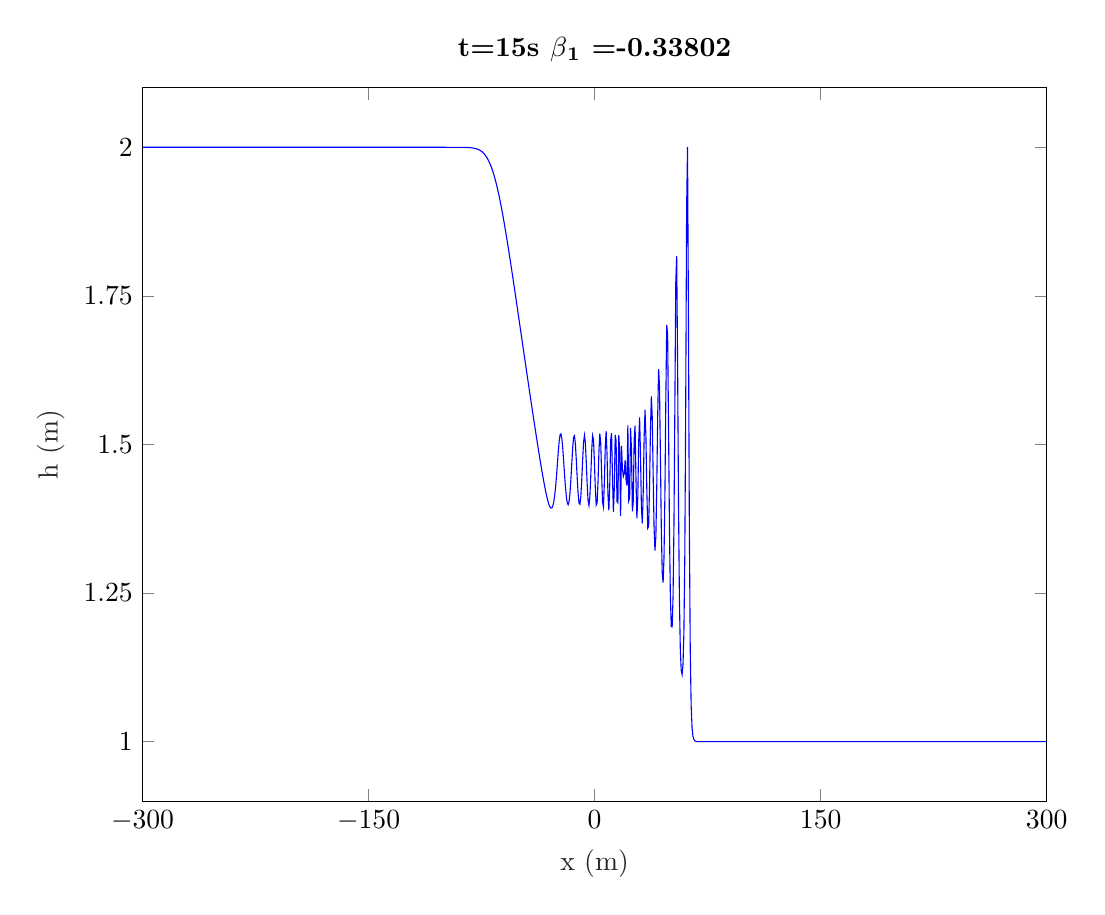
\begin{tikzpicture}

\begin{axis}[%
width=4.521in,
height=3.566in,
at={(0.758in,0.481in)},
scale only axis,
xmin=-300,
xmax=300,
xtick={-300, -150,    0,  150,  300},
xlabel style={font=\color{white!15!black}},
xlabel={x (m)},
ymin=0.9,
ymax=2.1,
ytick={   1, 1.25,  1.5, 1.75,    2},
ylabel style={font=\color{white!15!black}},
ylabel={h (m)},
axis background/.style={fill=white},
title style={font=\bfseries},
title={$\text{t=15s   }\beta{}_\text{1}\text{ =-0.33802}$}
]
\addplot [color=blue, forget plot]
  table[row sep=crcr]{%
-300.18000900045	2\\
-299.57997899895	2\\
-298.97994899745	2\\
-298.37991899595	2\\
-297.77988899445	2\\
-297.17985899295	2\\
-296.57982899145	2\\
-295.979798989949	2\\
-295.379768988449	2\\
-294.779738986949	2\\
-294.179708985449	2\\
-293.579678983949	2\\
-292.979648982449	2\\
-292.379618980949	2\\
-291.779588979449	2\\
-291.179558977949	2\\
-290.579528976449	2\\
-289.979498974949	2\\
-289.379468973449	2\\
-288.779438971949	2\\
-288.179408970449	2\\
-287.579378968948	2\\
-286.979348967448	2\\
-286.379318965948	2\\
-285.779288964448	2\\
-285.179258962948	2\\
-284.579228961448	2\\
-283.979198959948	2\\
-283.379168958448	2\\
-282.779138956948	2\\
-282.179108955448	2\\
-281.579078953948	2\\
-280.979048952448	2\\
-280.379018950948	2\\
-279.778988949447	2\\
-279.178958947947	2\\
-278.578928946447	2\\
-277.978898944947	2\\
-277.378868943447	2\\
-276.778838941947	2\\
-276.178808940447	2\\
-275.578778938947	2\\
-274.978748937447	2\\
-274.378718935947	2\\
-273.778688934447	2\\
-273.178658932947	2\\
-272.578628931447	2\\
-271.978598929946	2\\
-271.378568928446	2\\
-270.778538926946	2\\
-270.178508925446	2\\
-269.578478923946	2\\
-268.978448922446	2\\
-268.378418920946	2\\
-267.778388919446	2\\
-267.178358917946	2\\
-266.578328916446	2\\
-265.978298914946	2\\
-265.378268913446	2\\
-264.778238911946	2\\
-264.178208910446	2\\
-263.578178908945	2\\
-262.978148907445	2\\
-262.378118905945	2\\
-261.778088904445	2\\
-261.178058902945	2\\
-260.578028901445	2\\
-259.977998899945	2\\
-259.377968898445	2\\
-258.777938896945	2\\
-258.177908895445	2\\
-257.577878893945	2\\
-256.977848892445	2\\
-256.377818890945	2\\
-255.777788889444	2\\
-255.177758887944	2\\
-254.577728886444	2\\
-253.977698884944	2\\
-253.377668883444	2\\
-252.777638881944	2\\
-252.177608880444	2\\
-251.577578878944	2\\
-250.977548877444	2\\
-250.377518875944	2\\
-249.777488874444	2\\
-249.177458872944	2\\
-248.577428871444	2\\
-247.977398869943	2\\
-247.377368868443	2\\
-246.777338866943	2\\
-246.177308865443	2\\
-245.577278863943	2\\
-244.977248862443	2\\
-244.377218860943	2\\
-243.777188859443	2\\
-243.177158857943	2\\
-242.577128856443	2\\
-241.977098854943	2\\
-241.377068853443	2\\
-240.777038851943	2\\
-240.177008850443	2\\
-239.576978848942	2\\
-238.976948847442	2\\
-238.376918845942	2\\
-237.776888844442	2\\
-237.176858842942	2\\
-236.576828841442	2\\
-235.976798839942	2\\
-235.376768838442	2\\
-234.776738836942	2\\
-234.176708835442	2\\
-233.576678833942	2\\
-232.976648832442	2\\
-232.376618830942	2\\
-231.776588829441	2\\
-231.176558827941	2\\
-230.576528826441	2\\
-229.976498824941	2\\
-229.376468823441	2\\
-228.776438821941	2\\
-228.176408820441	2\\
-227.576378818941	2\\
-226.976348817441	2\\
-226.376318815941	2\\
-225.776288814441	2\\
-225.176258812941	2\\
-224.576228811441	2\\
-223.976198809941	2\\
-223.37616880844	2\\
-222.77613880694	2\\
-222.17610880544	2\\
-221.57607880394	2\\
-220.97604880244	2\\
-220.37601880094	2\\
-219.77598879944	2\\
-219.17595879794	2\\
-218.57592879644	2\\
-217.97589879494	2\\
-217.37586879344	2\\
-216.77583879194	2\\
-216.17580879044	2\\
-215.575778788939	2\\
-214.975748787439	2\\
-214.375718785939	2\\
-213.775688784439	2\\
-213.175658782939	2\\
-212.575628781439	2\\
-211.975598779939	2\\
-211.375568778439	2\\
-210.775538776939	2\\
-210.175508775439	2\\
-209.575478773939	2\\
-208.975448772439	2\\
-208.375418770939	2\\
-207.775388769438	2\\
-207.175358767938	2\\
-206.575328766438	2\\
-205.975298764938	2\\
-205.375268763438	2\\
-204.775238761938	2\\
-204.175208760438	2\\
-203.575178758938	2\\
-202.975148757438	2\\
-202.375118755938	2\\
-201.775088754438	2\\
-201.175058752938	2\\
-200.575028751438	2\\
-199.974998749937	2\\
-199.374968748437	2\\
-198.774938746937	2\\
-198.174908745437	2\\
-197.574878743937	2\\
-196.974848742437	2\\
-196.374818740937	2\\
-195.774788739437	2\\
-195.174758737937	2\\
-194.574728736437	2\\
-193.974698734937	2\\
-193.374668733437	2\\
-192.774638731937	2\\
-192.174608730437	2\\
-191.574578728936	2\\
-190.974548727436	2\\
-190.374518725936	2\\
-189.774488724436	2\\
-189.174458722936	2\\
-188.574428721436	2\\
-187.974398719936	2\\
-187.374368718436	2\\
-186.774338716936	2\\
-186.174308715436	2\\
-185.574278713936	2\\
-184.974248712436	2\\
-184.374218710936	2\\
-183.774188709435	2\\
-183.174158707935	2\\
-182.574128706435	2\\
-181.974098704935	2\\
-181.374068703435	2\\
-180.774038701935	2\\
-180.174008700435	2\\
-179.573978698935	2\\
-178.973948697435	2\\
-178.373918695935	2\\
-177.773888694435	2\\
-177.173858692935	2\\
-176.573828691435	2\\
-175.973798689934	2\\
-175.373768688434	2\\
-174.773738686934	2\\
-174.173708685434	2\\
-173.573678683934	2\\
-172.973648682434	2\\
-172.373618680934	2\\
-171.773588679434	2\\
-171.173558677934	2\\
-170.573528676434	2\\
-169.973498674934	2\\
-169.373468673434	2\\
-168.773438671934	2\\
-168.173408670434	2\\
-167.573378668933	2\\
-166.973348667433	2\\
-166.373318665933	2\\
-165.773288664433	2\\
-165.173258662933	2\\
-164.573228661433	2\\
-163.973198659933	2\\
-163.373168658433	2\\
-162.773138656933	2\\
-162.173108655433	2\\
-161.573078653933	2\\
-160.973048652433	2\\
-160.373018650933	2\\
-159.772988649432	2\\
-159.172958647932	2\\
-158.572928646432	2\\
-157.972898644932	2\\
-157.372868643432	2\\
-156.772838641932	2\\
-156.172808640432	2\\
-155.572778638932	2\\
-154.972748637432	2\\
-154.372718635932	2\\
-153.772688634432	2\\
-153.172658632932	2\\
-152.572628631432	2\\
-151.972598629931	2\\
-151.372568628431	2\\
-150.772538626931	2\\
-150.172508625431	2\\
-149.572478623931	2\\
-148.972448622431	2\\
-148.372418620931	2\\
-147.772388619431	2\\
-147.172358617931	2\\
-146.572328616431	2\\
-145.972298614931	2\\
-145.372268613431	2\\
-144.772238611931	2\\
-144.172208610431	2\\
-143.57217860893	2\\
-142.97214860743	2\\
-142.37211860593	2\\
-141.77208860443	2\\
-141.17205860293	2\\
-140.57202860143	2\\
-139.97199859993	2\\
-139.37196859843	2\\
-138.77193859693	2\\
-138.17190859543	2\\
-137.57187859393	2\\
-136.97184859243	2\\
-136.37181859093	2\\
-135.771788589429	2\\
-135.171758587929	2\\
-134.571728586429	2\\
-133.971698584929	2\\
-133.371668583429	2\\
-132.771638581929	1.99999999999999\\
-132.171608580429	1.99999999999998\\
-131.571578578929	1.99999999999996\\
-130.971548577429	1.99999999999994\\
-130.371518575929	1.99999999999991\\
-129.771488574429	1.99999999999986\\
-129.171458572929	1.9999999999998\\
-128.571428571429	1.99999999999972\\
-127.971398569929	1.99999999999961\\
-127.371368568428	1.99999999999945\\
-126.771338566928	1.99999999999923\\
-126.171308565428	1.99999999999893\\
-125.571278563928	1.99999999999852\\
-124.971248562428	1.99999999999796\\
-124.371218560928	1.99999999999718\\
-123.771188559428	1.9999999999961\\
-123.171158557928	1.99999999999463\\
-122.571128556428	1.99999999999261\\
-121.971098554928	1.99999999998984\\
-121.371068553428	1.99999999998605\\
-120.771038551928	1.99999999998087\\
-120.171008550428	1.99999999997379\\
-119.570978548927	1.99999999996414\\
-118.970948547427	1.99999999995097\\
-118.370918545927	1.99999999993303\\
-117.770888544427	1.99999999990864\\
-117.170858542927	1.9999999998755\\
-116.570828541427	1.99999999983051\\
-115.970798539927	1.99999999976951\\
-115.370768538427	1.9999999996869\\
-114.770738536927	1.99999999957515\\
-114.170708535427	1.99999999942417\\
-113.570678533927	1.9999999992204\\
-112.970648532427	1.99999999894575\\
-112.370618530927	1.99999999857598\\
-111.770588529426	1.99999999807878\\
-111.170558527926	1.99999999741106\\
-110.570528526426	1.99999999651548\\
-109.970498524926	1.99999999531584\\
-109.370468523426	1.99999999371097\\
-108.770438521926	1.99999999156686\\
-108.170408520426	1.99999998870615\\
-107.570378518926	1.99999998489454\\
-106.970348517426	1.99999997982299\\
-106.370318515926	1.99999997308451\\
-105.770288514426	1.99999996414397\\
-105.170258512926	1.99999995229894\\
-104.570228511426	1.99999993662898\\
-103.970198509925	1.99999991592995\\
-103.370168508425	1.99999988862941\\
-102.770138506925	1.99999985267759\\
-102.170108505425	1.99999980540739\\
-101.570078503925	1.99999974335485\\
-100.970048502425	1.99999966202964\\
-100.370018500925	1.99999955562219\\
-99.769988499425	1.99999941663097\\
-99.1699584979249	1.99999923538931\\
-98.5699284964248	1.99999899946621\\
-97.9698984949247	1.99999869290964\\
-97.3698684934247	1.99999829529349\\
-96.7698384919246	1.99999778052071\\
-96.1698084904245	1.99999711532452\\
-95.5697784889244	1.99999625739739\\
-94.9697484874244	1.99999515306256\\
-94.3697184859243	1.99999373438577\\
-93.7696884844242	1.99999191560472\\
-93.1696584829241	1.99998958873084\\
-92.5696284814241	1.99998661815127\\
-91.969598479924	1.99998283402969\\
-91.3695684784239	1.99997802427093\\
-90.7695384769239	1.99997192477872\\
-90.1695084754238	1.99996420769657\\
-89.5694784739237	1.99995446728143\\
-88.9694484724236	1.99994220301821\\
-88.3694184709235	1.99992679954358\\
-87.7693884694235	1.99990750291102\\
-87.1693584679234	1.99988339270032\\
-86.5693284664233	1.99985334945697\\
-85.9692984649232	1.9998160169465\\
-85.3692684634232	1.99976975873116\\
-84.7692384619231	1.9997126086306\\
-84.169208460423	1.99964221472143\\
-83.5691784589229	1.99955577667366\\
-82.9691484574229	1.9994499764249\\
-82.3691184559228	1.99932090246452\\
-81.7690884544227	1.99916396835006\\
-81.1690584529227	1.99897382651202\\
-80.5690284514226	1.9987442789232\\
-79.9689984499225	1.99846818681141\\
-79.3689684484224	1.99813738226729\\
-78.7689384469223	1.99774258531946\\
-78.1689084454223	1.99727333078344\\
-77.5688784439222	1.99671790988827\\
-76.9688484424221	1.99606333228392\\
-76.368818440922	1.99529531445694\\
-75.768788439422	1.99439830074463\\
-75.1687584379219	1.99335552295133\\
-74.5687284364218	1.99214910394888\\
-73.9686984349217	1.99076020951942\\
-73.3686684334217	1.98916925103454\\
-72.7686384319216	1.98735613936621\\
-72.1686084304215	1.98530058775191\\
-71.5685784289215	1.98298245831529\\
-70.9685484274214	1.98038214376121\\
-70.3685184259213	1.97748097266669\\
-69.7684884244212	1.97426162406013\\
-69.1684584229211	1.97070853491296\\
-68.5684284214211	1.96680828302911\\
-67.968398419921	1.96254992781419\\
-67.3683684184209	1.95792529264479\\
-66.7683384169208	1.95292917502645\\
-66.1683084154208	1.94755947427958\\
-65.5682784139207	1.94181723085967\\
-64.9682484124206	1.93570657623856\\
-64.3682184109205	1.92923459713339\\
-63.7681884094205	1.92241112235401\\
-63.1681584079204	1.91524844428129\\
-62.5681284064203	1.90776098971534\\
-61.9680984049203	1.89996495638698\\
-61.3680684034202	1.89187793178324\\
-60.7680384019201	1.88351851018903\\
-60.16800840042	1.87490592218012\\
-59.5679783989199	1.86605968846652\\
-58.9679483974199	1.85699930725338\\
-58.3679183959198	1.84774398142453\\
-57.7678883944197	1.8383123890921\\
-57.1678583929196	1.8287224985724\\
-56.5678283914196	1.81899142676236\\
-55.9677983899195	1.80913533826326\\
-55.3677683884194	1.7991693814396\\
-54.7677383869193	1.78910765688209\\
-54.1677083854193	1.77896321340965\\
-53.5676783839192	1.76874806672548\\
-52.9676483824191	1.75847323606384\\
-52.3676183809191	1.74814879455435\\
-51.767588379419	1.73778392952716\\
-51.1675583779189	1.72738700953422\\
-50.5675283764188	1.71696565542632\\
-49.9674983749187	1.70652681337669\\
-49.3674683734187	1.69607682825884\\
-48.7674383719186	1.68562151625909\\
-48.1674083704185	1.67516623603066\\
-47.5673783689184	1.66471595807614\\
-46.9673483674184	1.6542753323861\\
-46.3673183659183	1.6438487546719\\
-45.7672883644182	1.63344043182169\\
-45.1672583629181	1.62305444749532\\
-44.5672283614181	1.6126948290718\\
-43.967198359918	1.60236561749336\\
-43.3671683584179	1.5920709419366\\
-42.7671383569178	1.58181510171535\\
-42.1671083554178	1.57160265841947\\
-41.5670783539177	1.56143854207221\\
-40.9670483524176	1.55132817611174\\
-40.3670183509175	1.54127762736459\\
-39.7669883494175	1.53129378900355\\
-39.1669583479174	1.52138460694359\\
-38.5669283464173	1.51155936346419\\
-37.9668983449172	1.50182903638293\\
-37.3668683434172	1.49220675829825\\
-36.7668383419171	1.48270840888976\\
-36.166808340417	1.47335338485868\\
-35.5667783389169	1.46416560793166\\
-34.9667483374168	1.45517485288085\\
-34.3667183359168	1.44641850646499\\
-33.7666883344167	1.43794390638061\\
-33.1666583329167	1.42981145797713\\
-32.5666283314166	1.42209878470999\\
-31.9665983299165	1.41490622940227\\
-31.3665683284164	1.40836406736446\\
-30.7665383269164	1.40264177097257\\
-30.1665083254163	1.39795947374728\\
-29.5664783239162	1.39460121119916\\
-28.9664483224161	1.39292818064262\\
-28.3664183209161	1.39338756919048\\
-27.766388319416	1.39650729621773\\
-27.1663583179159	1.40285979131384\\
-26.5663283164158	1.41296719365518\\
-25.9662983149157	1.42711585235032\\
-25.3662683134157	1.44506173025347\\
-24.7662383119156	1.46566861715929\\
-24.1662083104155	1.48663987322292\\
-23.5661783089154	1.50462826139205\\
-22.9661483074154	1.51597026381354\\
-22.3661183059153	1.51793349686869\\
-21.7660883044152	1.50985610829344\\
-21.1660583029151	1.49343350633537\\
-20.5660283014151	1.4719826905199\\
-19.965998299915	1.44924444520874\\
-19.3659682984149	1.42845831340328\\
-18.7659382969148	1.41203553789067\\
-18.1659082954148	1.40169227132282\\
-17.5658782939147	1.39872406032999\\
-16.9658482924146	1.40412505242713\\
-16.3658182909145	1.41836572096029\\
-15.7657882894144	1.44067921550087\\
-15.1657582879144	1.46803870763275\\
-14.5657282864143	1.49451378678017\\
-13.9656982849143	1.51225409720707\\
-13.3656682834142	1.51470404668843\\
-12.7656382819141	1.50035536354712\\
-12.165608280414	1.47384604029667\\
-11.565578278914	1.44342312113154\\
-10.9655482774139	1.41726724968726\\
-10.3655182759138	1.40139519997255\\
-9.76548827441371	1.39940876731344\\
-9.16545827291367	1.41266457824382\\
-8.56542827141357	1.43953858616362\\
-7.96539826991352	1.4737068231945\\
-7.36536826841342	1.50346377408016\\
-6.76533826691332	1.51546385714305\\
-6.16530826541327	1.50289982978893\\
-5.56527826391317	1.47102994917117\\
-4.96524826241313	1.43386763034002\\
-4.36521826091303	1.40602943140897\\
-3.76518825941298	1.39750324319059\\
-3.16515825791288	1.41229391381176\\
-2.56512825641283	1.44712441860691\\
-1.96509825491273	1.48867255932115\\
-1.36506825341269	1.51503699435981\\
-0.765038251912586	1.50855302524114\\
-0.165008250412541	1.47181332253678\\
0.435021751087561	1.42675268088633\\
1.03505175258761	1.39816092115644\\
1.63508175408771	1.40112349491201\\
2.23511175558775	1.43657932280986\\
2.83514175708785	1.48713164371473\\
3.43517175858796	1.51836394260016\\
4.035201760088	1.50292594247254\\
4.6352317615881	1.4512709221857\\
5.23526176308815	1.4035622799879\\
5.83529176458825	1.39480411613536\\
6.43532176608829	1.43418874669364\\
7.03535176758839	1.49549933257811\\
7.63538176908844	1.52228405057271\\
8.23541177058854	1.48218258190621\\
8.83544177208859	1.41521583687158\\
9.43547177358869	1.3890542727468\\
10.0355017750887	1.43281602174845\\
10.6355317765888	1.5070216547492\\
11.2355617780889	1.51907553156989\\
11.835591779589	1.4455458060431\\
12.435621781089	1.38619871451483\\
13.0356517825891	1.42488514643762\\
13.6356817840892	1.51594774522592\\
14.2357117855893	1.50630619990364\\
14.8357417870894	1.40401329567157\\
15.4357717885894	1.4018438558566\\
16.0358017900895	1.51570469615717\\
16.6358317915896	1.48785598522333\\
17.2358617930897	1.38003938777492\\
17.8358917945897	1.49771476442273\\
18.4359217960898	1.45895141132846\\
19.0359517975899	1.44607367232158\\
19.63598179909	1.45108097722884\\
20.23601180059	1.47354846281987\\
20.8360418020901	1.44050405544269\\
21.4360718035902	1.43094533139173\\
22.0361018050903	1.53207756386655\\
22.6361318065904	1.40549077876717\\
23.2361618080904	1.4104559741628\\
23.8361918095905	1.52798153162815\\
24.4362218110905	1.49209513257363\\
25.0362518125906	1.38733065438242\\
25.6362818140907	1.40502582987409\\
26.2363118155908	1.50942538819862\\
26.8363418170908	1.53160210450706\\
27.4363718185909	1.44080442810601\\
28.036401820091	1.37548776994604\\
28.6364318215911	1.41125810999885\\
29.2364618230911	1.50544132357263\\
29.8364918245912	1.54541968895742\\
30.4365218260913	1.48176424244007\\
31.0365518275914	1.39418045130103\\
31.6365818290914	1.36733898094448\\
32.2366118305915	1.41977492473232\\
32.8366418320916	1.51085625178426\\
33.4366718335917	1.55804490083806\\
34.0367018350918	1.51269900838569\\
34.6367318365918	1.42145061864487\\
35.2367618380919	1.35933427064855\\
35.836791839592	1.36223366308756\\
36.4368218410921	1.42923777781664\\
37.0368518425921	1.52549835321972\\
37.6368818440922	1.58102553708487\\
38.2369118455923	1.54500879823558\\
38.8369418470924	1.4479411244934\\
39.4369718485924	1.35941882305099\\
40.0370018500925	1.32145804562503\\
40.6370318515926	1.34602827593732\\
41.2370618530927	1.43063570399529\\
41.8370918545928	1.54787983513702\\
42.4371218560928	1.62684687264892\\
43.0371518575929	1.5980815039451\\
43.6371818590929	1.48165417723707\\
44.237211860593	1.3595400765351\\
44.8372418620931	1.28426327326219\\
45.4372718635932	1.26740561684119\\
46.0373018650932	1.31069505448332\\
46.6373318665933	1.41858600898845\\
47.2373618680934	1.57554260104382\\
47.8373918695935	1.70109152335156\\
48.4374218710935	1.68433010622841\\
49.0374518725936	1.53200784934387\\
49.6374818740937	1.36094941623839\\
50.2375118755938	1.24606474801473\\
50.8375418770938	1.19386024098509\\
51.4375718785939	1.19315108295024\\
52.037601880094	1.24457173501336\\
52.6376318815941	1.36510993555388\\
53.2376618830942	1.56444962590339\\
53.8376918845942	1.77254947731731\\
54.4377218860943	1.81686819286788\\
55.0377518875944	1.64111065152011\\
55.6377818890945	1.40682286562982\\
56.2378118905945	1.24246209659653\\
56.8378418920946	1.15669574370205\\
57.4378718935947	1.12036281004277\\
58.0379018950948	1.11278807363946\\
58.6379318965948	1.12938007992657\\
59.2379618980949	1.18376587044111\\
59.837991899595	1.31366799575102\\
60.4380219010951	1.56855118010288\\
61.0380519025952	1.89746945178605\\
61.6380819040952	2.00072724397477\\
62.2381119055953	1.71888237408432\\
62.8381419070953	1.36614122985383\\
63.4381719085955	1.15521406352403\\
64.0382019100955	1.06115905188422\\
64.6382319115956	1.02364286020649\\
65.2382619130956	1.00917622088313\\
65.8382919145957	1.00360958354422\\
66.4383219160958	1.00144458107982\\
67.0383519175959	1.00058903868986\\
67.6383819190959	1.00024479352562\\
68.238411920596	1.00010365146211\\
68.8384419220961	1.00004468454459\\
69.4384719235962	1.00001959321386\\
70.0385019250962	1.00000872752968\\
70.6385319265963	1.00000394393067\\
71.2385619280964	1.00000180554633\\
71.8385919295965	1.00000083621633\\
72.4386219310966	1.00000039126338\\
73.0386519325966	1.00000018471655\\
73.6386819340967	1.00000008788585\\
74.2387119355968	1.00000004209679\\
74.8387419370969	1.00000002028089\\
75.4387719385969	1.00000000981914\\
76.038801940097	1.00000000477413\\
76.6388319415971	1.00000000232959\\
77.2388619430972	1.00000000114023\\
77.8388919445972	1.00000000055954\\
78.4389219460973	1.00000000027519\\
79.0389519475974	1.00000000013559\\
79.6389819490975	1.00000000006691\\
80.2390119505975	1.00000000003306\\
80.8390419520976	1.00000000001635\\
81.4390719535977	1.00000000000809\\
82.0391019550977	1.000000000004\\
82.6391319565979	1.00000000000198\\
83.2391619580979	1.00000000000098\\
83.839191959598	1.00000000000048\\
84.439221961098	1.00000000000024\\
85.0392519625981	1.00000000000011\\
85.6392819640982	1.00000000000005\\
86.2393119655983	1.00000000000002\\
86.8393419670983	1\\
87.4393719685984	1\\
88.0394019700985	1\\
88.6394319715986	1\\
89.2394619730986	1\\
89.8394919745987	1\\
90.4395219760988	1\\
91.0395519775989	1\\
91.639581979099	1\\
92.239611980599	1\\
92.8396419820991	1\\
93.4396719835992	1\\
94.0397019850993	1\\
94.6397319865993	1\\
95.2397619880994	1\\
95.8397919895995	1\\
96.4398219910996	1\\
97.0398519925996	1\\
97.6398819940997	1\\
98.2399119955998	1\\
98.8399419970999	1\\
99.4399719985999	1\\
100.0400020001	1\\
100.6400320016	1\\
101.2400620031	1\\
101.8400920046	1\\
102.4401220061	1\\
103.0401520076	1\\
103.6401820091	1\\
104.240212010601	1\\
104.840242012101	1\\
105.440272013601	1\\
106.040302015101	1\\
106.640332016601	1\\
107.240362018101	1\\
107.840392019601	1\\
108.440422021101	1\\
109.040452022601	1\\
109.640482024101	1\\
110.240512025601	1\\
110.840542027101	1\\
111.440572028601	1\\
112.040602030102	1\\
112.640632031602	1\\
113.240662033102	1\\
113.840692034602	1\\
114.440722036102	1\\
115.040752037602	1\\
115.640782039102	1\\
116.240812040602	1\\
116.840842042102	1\\
117.440872043602	1\\
118.040902045102	1\\
118.640932046602	1\\
119.240962048102	1\\
119.840992049603	1\\
120.441022051103	1\\
121.041052052603	1\\
121.641082054103	1\\
122.241112055603	1\\
122.841142057103	1\\
123.441172058603	1\\
124.041202060103	1\\
124.641232061603	1\\
125.241262063103	1\\
125.841292064603	1\\
126.441322066103	1\\
127.041352067603	1\\
127.641382069103	1\\
128.241412070604	1\\
128.841442072104	1\\
129.441472073604	1\\
130.041502075104	1\\
130.641532076604	1\\
131.241562078104	1\\
131.841592079604	1\\
132.441622081104	1\\
133.041652082604	1\\
133.641682084104	1\\
134.241712085604	1\\
134.841742087104	1\\
135.441772088604	1\\
136.041802090105	1\\
136.641832091605	1\\
137.241862093105	1\\
137.841892094605	1\\
138.441922096105	1\\
139.041952097605	1\\
139.641982099105	1\\
140.242012100605	1\\
140.842042102105	1\\
141.442072103605	1\\
142.042102105105	1\\
142.642132106605	1\\
143.242162108105	1\\
143.842192109605	1\\
144.442222111106	1\\
145.042252112606	1\\
145.642282114106	1\\
146.242312115606	1\\
146.842342117106	1\\
147.442372118606	1\\
148.042402120106	1\\
148.642432121606	1\\
149.242462123106	1\\
149.842492124606	1\\
150.442522126106	1\\
151.042552127606	1\\
151.642582129106	1\\
152.242612130607	1\\
152.842642132107	1\\
153.442672133607	1\\
154.042702135107	1\\
154.642732136607	1\\
155.242762138107	1\\
155.842792139607	1\\
156.442822141107	1\\
157.042852142607	1\\
157.642882144107	1\\
158.242912145607	1\\
158.842942147107	1\\
159.442972148607	1\\
160.043002150107	1\\
160.643032151608	1\\
161.243062153108	1\\
161.843092154608	1\\
162.443122156108	1\\
163.043152157608	1\\
163.643182159108	1\\
164.243212160608	1\\
164.843242162108	1\\
165.443272163608	1\\
166.043302165108	1\\
166.643332166608	1\\
167.243362168108	1\\
167.843392169608	1\\
168.443422171109	1\\
169.043452172609	1\\
169.643482174109	1\\
170.243512175609	1\\
170.843542177109	1\\
171.443572178609	1\\
172.043602180109	1\\
172.643632181609	1\\
173.243662183109	1\\
173.843692184609	1\\
174.443722186109	1\\
175.043752187609	1\\
175.643782189109	1\\
176.24381219061	1\\
176.84384219211	1\\
177.44387219361	1\\
178.04390219511	1\\
178.64393219661	1\\
179.24396219811	1\\
179.84399219961	1\\
180.44402220111	1\\
181.04405220261	1\\
181.64408220411	1\\
182.24411220561	1\\
182.84414220711	1\\
183.44417220861	1\\
184.04420221011	1\\
184.644232211611	1\\
185.244262213111	1\\
185.844292214611	1\\
186.444322216111	1\\
187.044352217611	1\\
187.644382219111	1\\
188.244412220611	1\\
188.844442222111	1\\
189.444472223611	1\\
190.044502225111	1\\
190.644532226611	1\\
191.244562228111	1\\
191.844592229611	1\\
192.444622231112	1\\
193.044652232612	1\\
193.644682234112	1\\
194.244712235612	1\\
194.844742237112	1\\
195.444772238612	1\\
196.044802240112	1\\
196.644832241612	1\\
197.244862243112	1\\
197.844892244612	1\\
198.444922246112	1\\
199.044952247612	1\\
199.644982249112	1\\
200.245012250613	1\\
200.845042252113	1\\
201.445072253613	1\\
202.045102255113	1\\
202.645132256613	1\\
203.245162258113	1\\
203.845192259613	1\\
204.445222261113	1\\
205.045252262613	1\\
205.645282264113	1\\
206.245312265613	1\\
206.845342267113	1\\
207.445372268613	1\\
208.045402270114	1\\
208.645432271614	1\\
209.245462273114	1\\
209.845492274614	1\\
210.445522276114	1\\
211.045552277614	1\\
211.645582279114	1\\
212.245612280614	1\\
212.845642282114	1\\
213.445672283614	1\\
214.045702285114	1\\
214.645732286614	1\\
215.245762288114	1\\
215.845792289614	1\\
216.445822291115	1\\
217.045852292615	1\\
217.645882294115	1\\
218.245912295615	1\\
218.845942297115	1\\
219.445972298615	1\\
220.046002300115	1\\
220.646032301615	1\\
221.246062303115	1\\
221.846092304615	1\\
222.446122306115	1\\
223.046152307615	1\\
223.646182309115	1\\
224.246212310616	1\\
224.846242312116	1\\
225.446272313616	1\\
226.046302315116	1\\
226.646332316616	1\\
227.246362318116	1\\
227.846392319616	1\\
228.446422321116	1\\
229.046452322616	1\\
229.646482324116	1\\
230.246512325616	1\\
230.846542327116	1\\
231.446572328616	1\\
232.046602330116	1\\
232.646632331617	1\\
233.246662333117	1\\
233.846692334617	1\\
234.446722336117	1\\
235.046752337617	1\\
235.646782339117	1\\
236.246812340617	1\\
236.846842342117	1\\
237.446872343617	1\\
238.046902345117	1\\
238.646932346617	1\\
239.246962348117	1\\
239.846992349617	1\\
240.447022351118	1\\
241.047052352618	1\\
241.647082354118	1\\
242.247112355618	1\\
242.847142357118	1\\
243.447172358618	1\\
244.047202360118	1\\
244.647232361618	1\\
245.247262363118	1\\
245.847292364618	1\\
246.447322366118	1\\
247.047352367618	1\\
247.647382369118	1\\
248.247412370619	1\\
248.847442372119	1\\
249.447472373619	1\\
250.047502375119	1\\
250.647532376619	1\\
251.247562378119	1\\
251.847592379619	1\\
252.447622381119	1\\
253.047652382619	1\\
253.647682384119	1\\
254.247712385619	1\\
254.847742387119	1\\
255.447772388619	1\\
256.04780239012	1\\
256.64783239162	1\\
257.24786239312	1\\
257.84789239462	1\\
258.44792239612	1\\
259.04795239762	1\\
259.64798239912	1\\
260.24801240062	1\\
260.84804240212	1\\
261.44807240362	1\\
262.04810240512	1\\
262.64813240662	1\\
263.24816240812	1\\
263.84819240962	1\\
264.448222411121	1\\
265.048252412621	1\\
265.648282414121	1\\
266.248312415621	1\\
266.848342417121	1\\
267.448372418621	1\\
268.048402420121	1\\
268.648432421621	1\\
269.248462423121	1\\
269.848492424621	1\\
270.448522426121	1\\
271.048552427621	1\\
271.648582429121	1\\
272.248612430622	1\\
272.848642432122	1\\
273.448672433622	1\\
274.048702435122	1\\
274.648732436622	1\\
275.248762438122	1\\
275.848792439622	1\\
276.448822441122	1\\
277.048852442622	1\\
277.648882444122	1\\
278.248912445622	1\\
278.848942447122	1\\
279.448972448622	1\\
280.049002450123	1\\
280.649032451623	1\\
281.249062453123	1\\
281.849092454623	1\\
282.449122456123	1\\
283.049152457623	1\\
283.649182459123	1\\
284.249212460623	1\\
284.849242462123	1\\
285.449272463623	1\\
286.049302465123	1\\
286.649332466623	1\\
287.249362468123	1\\
287.849392469623	1\\
288.449422471124	1\\
289.049452472624	1\\
289.649482474124	1\\
290.249512475624	1\\
290.849542477124	1\\
291.449572478624	1\\
292.049602480124	1\\
292.649632481624	1\\
293.249662483124	1\\
293.849692484624	1\\
294.449722486124	1\\
295.049752487624	1\\
295.649782489125	1\\
296.249812490625	1\\
296.849842492125	1\\
297.449872493625	1\\
298.049902495125	1\\
298.649932496625	1\\
299.249962498125	1\\
299.849992499625	1\\
};
\end{axis}
\end{tikzpicture}%
		\caption{$t=15s$}
	\end{subfigure}
	\begin{subfigure}{0.49\textwidth}
		\centering
		% This file was created by matlab2tikz.
%
%The latest updates can be retrieved from
%  http://www.mathworks.com/matlabcentral/fileexchange/22022-matlab2tikz-matlab2tikz
%where you can also make suggestions and rate matlab2tikz.
%
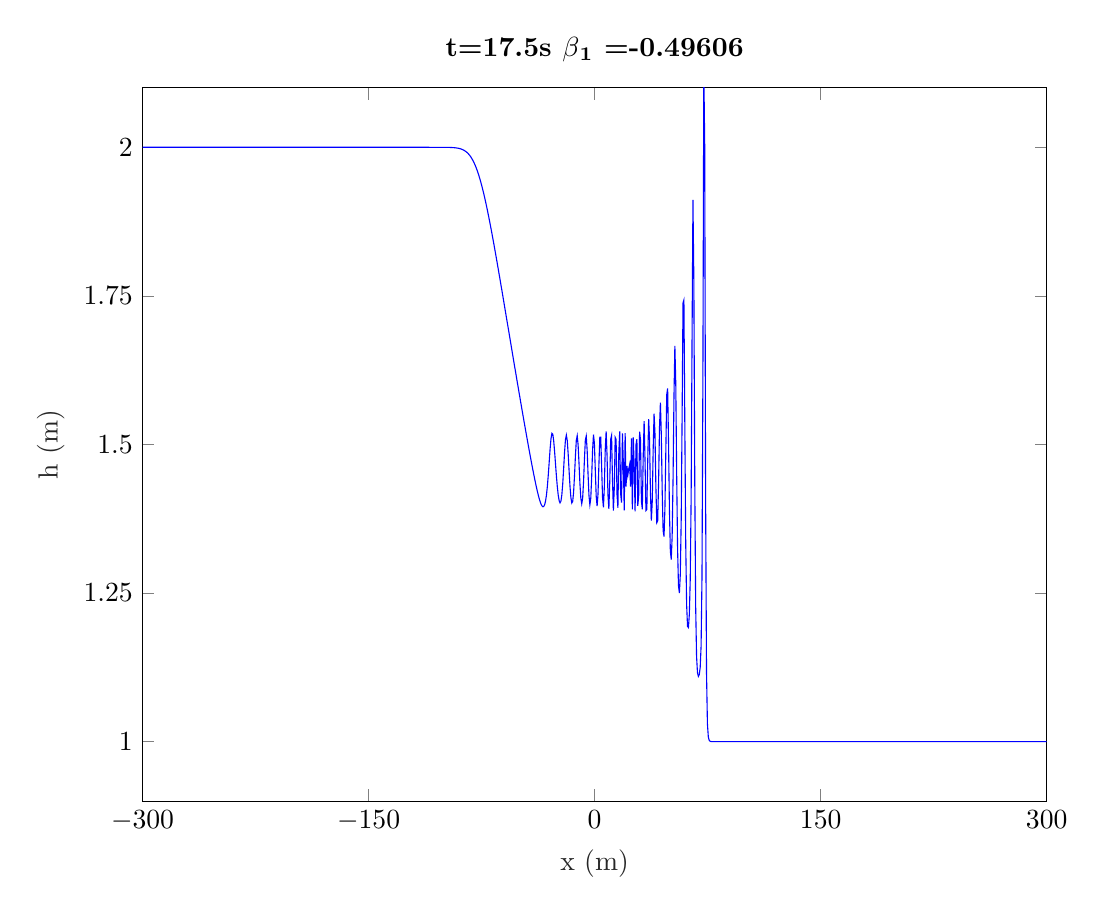
\begin{tikzpicture}

\begin{axis}[%
width=4.521in,
height=3.566in,
at={(0.758in,0.481in)},
scale only axis,
xmin=-300,
xmax=300,
xtick={-300, -150,    0,  150,  300},
xlabel style={font=\color{white!15!black}},
xlabel={x (m)},
ymin=0.9,
ymax=2.1,
ytick={   1, 1.25,  1.5, 1.75,    2},
ylabel style={font=\color{white!15!black}},
ylabel={h (m)},
axis background/.style={fill=white},
title style={font=\bfseries},
title={$\text{t=17.5s   }\beta{}_\text{1}\text{ =-0.49606}$}
]
\addplot [color=blue, forget plot]
  table[row sep=crcr]{%
-300.18000900045	2\\
-299.57997899895	2\\
-298.97994899745	2\\
-298.37991899595	2\\
-297.77988899445	2\\
-297.17985899295	2\\
-296.57982899145	2\\
-295.979798989949	2\\
-295.379768988449	2\\
-294.779738986949	2\\
-294.179708985449	2\\
-293.579678983949	2\\
-292.979648982449	2\\
-292.379618980949	2\\
-291.779588979449	2\\
-291.179558977949	2\\
-290.579528976449	2\\
-289.979498974949	2\\
-289.379468973449	2\\
-288.779438971949	2\\
-288.179408970449	2\\
-287.579378968948	2\\
-286.979348967448	2\\
-286.379318965948	2\\
-285.779288964448	2\\
-285.179258962948	2\\
-284.579228961448	2\\
-283.979198959948	2\\
-283.379168958448	2\\
-282.779138956948	2\\
-282.179108955448	2\\
-281.579078953948	2\\
-280.979048952448	2\\
-280.379018950948	2\\
-279.778988949447	2\\
-279.178958947947	2\\
-278.578928946447	2\\
-277.978898944947	2\\
-277.378868943447	2\\
-276.778838941947	2\\
-276.178808940447	2\\
-275.578778938947	2\\
-274.978748937447	2\\
-274.378718935947	2\\
-273.778688934447	2\\
-273.178658932947	2\\
-272.578628931447	2\\
-271.978598929946	2\\
-271.378568928446	2\\
-270.778538926946	2\\
-270.178508925446	2\\
-269.578478923946	2\\
-268.978448922446	2\\
-268.378418920946	2\\
-267.778388919446	2\\
-267.178358917946	2\\
-266.578328916446	2\\
-265.978298914946	2\\
-265.378268913446	2\\
-264.778238911946	2\\
-264.178208910446	2\\
-263.578178908945	2\\
-262.978148907445	2\\
-262.378118905945	2\\
-261.778088904445	2\\
-261.178058902945	2\\
-260.578028901445	2\\
-259.977998899945	2\\
-259.377968898445	2\\
-258.777938896945	2\\
-258.177908895445	2\\
-257.577878893945	2\\
-256.977848892445	2\\
-256.377818890945	2\\
-255.777788889444	2\\
-255.177758887944	2\\
-254.577728886444	2\\
-253.977698884944	2\\
-253.377668883444	2\\
-252.777638881944	2\\
-252.177608880444	2\\
-251.577578878944	2\\
-250.977548877444	2\\
-250.377518875944	2\\
-249.777488874444	2\\
-249.177458872944	2\\
-248.577428871444	2\\
-247.977398869943	2\\
-247.377368868443	2\\
-246.777338866943	2\\
-246.177308865443	2\\
-245.577278863943	2\\
-244.977248862443	2\\
-244.377218860943	2\\
-243.777188859443	2\\
-243.177158857943	2\\
-242.577128856443	2\\
-241.977098854943	2\\
-241.377068853443	2\\
-240.777038851943	2\\
-240.177008850443	2\\
-239.576978848942	2\\
-238.976948847442	2\\
-238.376918845942	2\\
-237.776888844442	2\\
-237.176858842942	2\\
-236.576828841442	2\\
-235.976798839942	2\\
-235.376768838442	2\\
-234.776738836942	2\\
-234.176708835442	2\\
-233.576678833942	2\\
-232.976648832442	2\\
-232.376618830942	2\\
-231.776588829441	2\\
-231.176558827941	2\\
-230.576528826441	2\\
-229.976498824941	2\\
-229.376468823441	2\\
-228.776438821941	2\\
-228.176408820441	2\\
-227.576378818941	2\\
-226.976348817441	2\\
-226.376318815941	2\\
-225.776288814441	2\\
-225.176258812941	2\\
-224.576228811441	2\\
-223.976198809941	2\\
-223.37616880844	2\\
-222.77613880694	2\\
-222.17610880544	2\\
-221.57607880394	2\\
-220.97604880244	2\\
-220.37601880094	2\\
-219.77598879944	2\\
-219.17595879794	2\\
-218.57592879644	2\\
-217.97589879494	2\\
-217.37586879344	2\\
-216.77583879194	2\\
-216.17580879044	2\\
-215.575778788939	2\\
-214.975748787439	2\\
-214.375718785939	2\\
-213.775688784439	2\\
-213.175658782939	2\\
-212.575628781439	2\\
-211.975598779939	2\\
-211.375568778439	2\\
-210.775538776939	2\\
-210.175508775439	2\\
-209.575478773939	2\\
-208.975448772439	2\\
-208.375418770939	2\\
-207.775388769438	2\\
-207.175358767938	2\\
-206.575328766438	2\\
-205.975298764938	2\\
-205.375268763438	2\\
-204.775238761938	2\\
-204.175208760438	2\\
-203.575178758938	2\\
-202.975148757438	2\\
-202.375118755938	2\\
-201.775088754438	2\\
-201.175058752938	2\\
-200.575028751438	2\\
-199.974998749937	2\\
-199.374968748437	2\\
-198.774938746937	2\\
-198.174908745437	2\\
-197.574878743937	2\\
-196.974848742437	2\\
-196.374818740937	2\\
-195.774788739437	2\\
-195.174758737937	2\\
-194.574728736437	2\\
-193.974698734937	2\\
-193.374668733437	2\\
-192.774638731937	2\\
-192.174608730437	2\\
-191.574578728936	2\\
-190.974548727436	2\\
-190.374518725936	2\\
-189.774488724436	2\\
-189.174458722936	2\\
-188.574428721436	2\\
-187.974398719936	2\\
-187.374368718436	2\\
-186.774338716936	2\\
-186.174308715436	2\\
-185.574278713936	2\\
-184.974248712436	2\\
-184.374218710936	2\\
-183.774188709435	2\\
-183.174158707935	2\\
-182.574128706435	2\\
-181.974098704935	2\\
-181.374068703435	2\\
-180.774038701935	2\\
-180.174008700435	2\\
-179.573978698935	2\\
-178.973948697435	2\\
-178.373918695935	2\\
-177.773888694435	2\\
-177.173858692935	2\\
-176.573828691435	2\\
-175.973798689934	2\\
-175.373768688434	2\\
-174.773738686934	2\\
-174.173708685434	2\\
-173.573678683934	2\\
-172.973648682434	2\\
-172.373618680934	2\\
-171.773588679434	2\\
-171.173558677934	2\\
-170.573528676434	2\\
-169.973498674934	2\\
-169.373468673434	2\\
-168.773438671934	2\\
-168.173408670434	2\\
-167.573378668933	2\\
-166.973348667433	2\\
-166.373318665933	2\\
-165.773288664433	2\\
-165.173258662933	2\\
-164.573228661433	2\\
-163.973198659933	2\\
-163.373168658433	2\\
-162.773138656933	2\\
-162.173108655433	2\\
-161.573078653933	2\\
-160.973048652433	2\\
-160.373018650933	2\\
-159.772988649432	2\\
-159.172958647932	2\\
-158.572928646432	2\\
-157.972898644932	2\\
-157.372868643432	2\\
-156.772838641932	2\\
-156.172808640432	2\\
-155.572778638932	2\\
-154.972748637432	2\\
-154.372718635932	2\\
-153.772688634432	2\\
-153.172658632932	2\\
-152.572628631432	2\\
-151.972598629931	2\\
-151.372568628431	2\\
-150.772538626931	2\\
-150.172508625431	2\\
-149.572478623931	2\\
-148.972448622431	2\\
-148.372418620931	2\\
-147.772388619431	2\\
-147.172358617931	2\\
-146.572328616431	2\\
-145.972298614931	2\\
-145.372268613431	2\\
-144.772238611931	2\\
-144.172208610431	1.99999999999999\\
-143.57217860893	1.99999999999998\\
-142.97214860743	1.99999999999997\\
-142.37211860593	1.99999999999995\\
-141.77208860443	1.99999999999992\\
-141.17205860293	1.99999999999987\\
-140.57202860143	1.99999999999982\\
-139.97199859993	1.99999999999974\\
-139.37196859843	1.99999999999963\\
-138.77193859693	1.99999999999948\\
-138.17190859543	1.99999999999928\\
-137.57187859393	1.999999999999\\
-136.97184859243	1.99999999999863\\
-136.37181859093	1.9999999999981\\
-135.771788589429	1.99999999999739\\
-135.171758587929	1.9999999999964\\
-134.571728586429	1.99999999999505\\
-133.971698584929	1.99999999999321\\
-133.371668583429	1.99999999999069\\
-132.771638581929	1.99999999998725\\
-132.171608580429	1.99999999998255\\
-131.571578578929	1.99999999997616\\
-130.971548577429	1.99999999996746\\
-130.371518575929	1.99999999995564\\
-129.771488574429	1.99999999993958\\
-129.171458572929	1.99999999991779\\
-128.571428571429	1.99999999988826\\
-127.971398569929	1.9999999998483\\
-127.371368568428	1.99999999979426\\
-126.771338566928	1.99999999972127\\
-126.171308565428	1.99999999962281\\
-125.571278563928	1.99999999949014\\
-124.971248562428	1.99999999931158\\
-124.371218560928	1.99999999907154\\
-123.771188559428	1.99999999874925\\
-123.171158557928	1.99999999831706\\
-122.571128556428	1.99999999773819\\
-121.971098554928	1.99999999696386\\
-121.371068553428	1.99999999592939\\
-120.771038551928	1.99999999454916\\
-120.171008550428	1.99999999271002\\
-119.570978548927	1.99999999026268\\
-118.970948547427	1.99999998701037\\
-118.370918545927	1.99999998269425\\
-117.770888544427	1.99999997697436\\
-117.170858542927	1.99999996940479\\
-116.570828541427	1.99999995940177\\
-115.970798539927	1.99999994620223\\
-115.370768538427	1.99999992881046\\
-114.770738536927	1.99999990592937\\
-114.170708535427	1.99999987587227\\
-113.570678533927	1.99999983644982\\
-112.970648532427	1.99999978482531\\
-112.370618530927	1.99999971733021\\
-111.770588529426	1.99999962922918\\
-111.170558527926	1.99999951442175\\
-110.570528526426	1.9999993650643\\
-109.970498524926	1.99999917109244\\
-109.370468523426	1.99999891961897\\
-108.770438521926	1.99999859417704\\
-108.170408520426	1.99999817377149\\
-107.570378518926	1.99999763169292\\
-106.970348517426	1.99999693403971\\
-106.370318515926	1.99999603788158\\
-105.770288514426	1.99999488898501\\
-105.170258512926	1.99999341900537\\
-104.570228511426	1.99999154203244\\
-103.970198509925	1.99998915035574\\
-103.370168508425	1.99998610929292\\
-102.770138506925	1.99998225089844\\
-102.170108505425	1.99997736634175\\
-101.570078503925	1.99997119671349\\
-100.970048502425	1.99996342198598\\
-100.370018500925	1.99995364782165\\
-99.769988499425	1.99994138989054\\
-99.1699584979249	1.99992605532853\\
-98.5699284964248	1.99990692094301\\
-97.9698984949247	1.99988310775623\\
-97.3698684934247	1.99985355147231\\
-96.7698384919246	1.99981696846698\\
-96.1698084904245	1.99977181693508\\
-95.5697784889244	1.9997162528972\\
-94.9697484874244	1.99964808087039\\
-94.3697184859243	1.99956469915712\\
-93.7696884844242	1.9994630399093\\
-93.1696584829241	1.99933950438795\\
-92.5696284814241	1.99918989416868\\
-91.969598479924	1.99900933944268\\
-91.3695684784239	1.9987922260285\\
-90.7695384769239	1.99853212323597\\
-90.1695084754238	1.99822171529143\\
-89.5694784739237	1.99785273961952\\
-88.9694484724236	1.99741593584222\\
-88.3694184709235	1.99690100985343\\
-87.7693884694235	1.99629661769656\\
-87.1693584679234	1.9955903741467\\
-86.5693284664233	1.9947688908052\\
-85.9692984649232	1.99381784808565\\
-85.3692684634232	1.99272210464911\\
-84.7692384619231	1.991465846601\\
-84.169208460423	1.99003277709174\\
-83.5691784589229	1.98840634491487\\
-82.9691484574229	1.98657000836293\\
-82.3691184559228	1.98450752813125\\
-81.7690884544227	1.98220328064266\\
-81.1690584529227	1.97964258102387\\
-80.5690284514226	1.97681200332467\\
-79.9689984499225	1.9736996846419\\
-79.3689684484224	1.97029559974819\\
-78.7689384469223	1.96659179371057\\
-78.1689084454223	1.96258256180051\\
-77.5688784439222	1.95826456862855\\
-76.9688484424221	1.95363690167476\\
-76.368818440922	1.94870105795509\\
-75.768788439422	1.94346086615104\\
-75.1687584379219	1.93792234983071\\
-74.5687284364218	1.93209354013848\\
-73.9686984349217	1.92598424833647\\
-73.3686684334217	1.91960580974117\\
-72.7686384319216	1.91297081090439\\
-72.1686084304215	1.90609281141326\\
-71.5685784289215	1.89898607056896\\
-70.9685484274214	1.89166528762593\\
-70.3685184259213	1.88414536242333\\
-69.7684884244212	1.87644118130072\\
-69.1684584229211	1.86856743131399\\
-68.5684284214211	1.86053844407293\\
-67.968398419921	1.85236806908675\\
-67.3683684184209	1.84406957536426\\
-66.7683384169208	1.83565557918009\\
-66.1683084154208	1.8271379953662\\
-65.5682784139207	1.81852800918496\\
-64.9682484124206	1.80983606574154\\
-64.3682184109205	1.80107187395369\\
-63.7681884094205	1.79224442227109\\
-63.1681584079204	1.78336200358476\\
-62.5681284064203	1.77443224705883\\
-61.9680984049203	1.76546215492374\\
-61.3680684034202	1.7564581425755\\
-60.7680384019201	1.74742608061576\\
-60.16800840042	1.7383713377338\\
-59.5679783989199	1.72929882357152\\
-58.9679483974199	1.7202130309225\\
-58.3679183959198	1.71111807679961\\
-57.7678883944197	1.70201774206185\\
-57.1678583929196	1.69291550942506\\
-56.5678283914196	1.68381459979475\\
-55.9677983899195	1.6747180069569\\
-55.3677683884194	1.66562853074688\\
-54.7677383869193	1.65654880889203\\
-54.1677083854193	1.6474813477927\\
-53.5676783839192	1.63842855257414\\
-52.9676483824191	1.62939275681024\\
-52.3676183809191	1.62037625239552\\
-51.767588379419	1.61138132012795\\
-51.1675583779189	1.60241026166773\\
-50.5675283764188	1.59346543366449\\
-49.9674983749187	1.5845492850059\\
-49.3674683734187	1.57566439834584\\
-48.7674383719186	1.56681353733741\\
-48.1674083704185	1.55799970134432\\
-47.5673783689184	1.54922618986333\\
-46.9673483674184	1.54049667949891\\
-46.3673183659183	1.53181531714245\\
-45.7672883644182	1.52318683409762\\
-45.1672583629181	1.51461668736524\\
-44.5672283614181	1.50611123630282\\
-43.967198359918	1.49767796561816\\
-43.3671683584179	1.48932576944222\\
-42.7671383569178	1.48106531649\\
-42.1671083554178	1.47290952368398\\
-41.5670783539177	1.46487417598997\\
-40.9670483524176	1.45697874490591\\
-40.3670183509175	1.44924747892726\\
-39.7669883494175	1.44171086903531\\
-39.1669583479174	1.43440763445363\\
-38.5669283464173	1.42738743330527\\
-37.9668983449172	1.4207145847842\\
-37.3668683434172	1.41447319836882\\
-36.7668383419171	1.40877423946553\\
-36.166808340417	1.40376519780601\\
-35.5667783389169	1.39964309118575\\
-34.9667483374168	1.3966713369773\\
-34.3667183359168	1.39520009762637\\
-33.7666883344167	1.39568716012545\\
-33.1666583329167	1.39870991543726\\
-32.5666283314166	1.40494800445031\\
-31.9665983299165	1.41509470447455\\
-31.3665683284164	1.42963538544697\\
-30.7665383269164	1.44843653797783\\
-30.1665083254163	1.47018667371779\\
-29.5664783239162	1.49197599352373\\
-28.9664483224161	1.50956976540073\\
-28.3664183209161	1.51876631406555\\
-27.766388319416	1.51731481317552\\
-27.1663583179159	1.50599561687593\\
-26.5663283164158	1.48797944671243\\
-25.9662983149157	1.46715003264457\\
-25.3662683134157	1.44673175658267\\
-24.7662383119156	1.42885241283358\\
-24.1662083104155	1.41479511206987\\
-23.5661783089154	1.40546027038825\\
-22.9661483074154	1.40173633106374\\
-22.3661183059153	1.40467219841157\\
-21.7660883044152	1.41529905585369\\
-21.1660583029151	1.43402124968675\\
-20.5660283014151	1.4593829321548\\
-19.965998299915	1.48671304464668\\
-19.3659682984149	1.5081651657666\\
-18.7659382969148	1.51580396619586\\
-18.1659082954148	1.50651209103577\\
-17.5658782939147	1.48400626245832\\
-16.9658482924146	1.45603484199532\\
-16.3658182909145	1.42998691387593\\
-15.7657882894144	1.41084669104093\\
-15.1657582879144	1.4015812422338\\
-14.5657282864143	1.40414649792944\\
-13.9656982849143	1.41964492574281\\
-13.3656682834142	1.44692906812534\\
-12.7656382819141	1.47998858354145\\
-12.165608280414	1.50690409345807\\
-11.565578278914	1.51476667163522\\
-10.9655482774139	1.49917103479368\\
-10.3655182759138	1.46790113859749\\
-9.76548827441371	1.43436453038293\\
-9.16545827291367	1.40963621937151\\
-8.56542827141357	1.40025246314784\\
-7.96539826991352	1.40945091516375\\
-7.36536826841342	1.43691147760046\\
-6.76533826691332	1.47533706498954\\
-6.16530826541327	1.5076283671154\\
-5.56527826391317	1.51423309857973\\
-4.96524826241313	1.49000118423568\\
-4.36521826091303	1.44964287403362\\
-3.76518825941298	1.41421587604044\\
-3.16515825791288	1.39854227104009\\
-2.56512825641283	1.40938596407841\\
-1.96509825491273	1.44514082407904\\
-1.36506825341269	1.49063176636576\\
-0.765038251912586	1.51668964878619\\
-0.165008250412541	1.50180412967644\\
0.435021751087561	1.45671809775446\\
1.03505175258761	1.41301959005233\\
1.63508175408771	1.39622626053159\\
2.23511175558775	1.41655967255366\\
2.83514175708785	1.46626099877251\\
3.43517175858796	1.51216801761388\\
4.035201760088	1.51211659199763\\
4.6352317615881	1.46390551058275\\
5.23526176308815	1.41080970151716\\
5.83529176458825	1.39434809310513\\
6.43532176608829	1.42864935845085\\
7.03535176758839	1.49149712620509\\
7.63538176908844	1.52194544520675\\
8.23541177058854	1.48153577362732\\
8.83544177208859	1.41513986770382\\
9.43547177358869	1.39170305034885\\
10.0355017750887	1.43669556917232\\
10.6355317765888	1.50890530555627\\
11.2355617780889	1.51511449210856\\
11.835591779589	1.44156144111288\\
12.435621781089	1.38881035039406\\
13.0356517825891	1.42662673771109\\
13.6356817840892	1.51195378030289\\
14.2357117855893	1.50870315594119\\
14.8357417870894	1.41633673489634\\
15.4357717885894	1.39354427001168\\
16.0358017900895	1.48569480708746\\
16.6358317915896	1.52206752638703\\
17.2358617930897	1.41736755385292\\
17.8358917945897	1.40214194635653\\
18.4359217960898	1.5186105691964\\
19.0359517975899	1.46956124220521\\
19.63598179909	1.3892978106272\\
20.23601180059	1.51889095652963\\
20.8360418020901	1.42931081432929\\
21.4360718035902	1.46405182132389\\
22.0361018050903	1.44850881949485\\
22.6361318065904	1.45910188480185\\
23.2361618080904	1.4664695176494\\
23.8361918095905	1.42903990686704\\
24.4362218110905	1.51008391213864\\
25.0362518125906	1.39068412649246\\
25.6362818140907	1.51203447149311\\
26.2363118155908	1.46379872132521\\
26.8363418170908	1.38729155982924\\
27.4363718185909	1.49960062585267\\
28.036401820091	1.50883356443743\\
28.6364318215911	1.39670487799348\\
29.2364618230911	1.41392947381636\\
29.8364918245912	1.5216752964361\\
30.4365218260913	1.5074974187439\\
31.0365518275914	1.40447390847055\\
31.6365818290914	1.39093259287973\\
32.2366118305915	1.48096579187859\\
32.8366418320916	1.53934271882457\\
33.4366718335917	1.47301835734538\\
34.0367018350918	1.38876786070475\\
34.6367318365918	1.39055993236132\\
35.2367618380919	1.47301581823199\\
35.836791839592	1.54273267653075\\
36.4368218410921	1.50778460322595\\
37.0368518425921	1.41758878211931\\
37.6368818440922	1.37205100004098\\
38.2369118455923	1.40484440550054\\
38.8369418470924	1.49100434506732\\
39.4369718485924	1.55193453185056\\
40.0370018500925	1.51803544508427\\
40.6370318515926	1.42909015366143\\
41.2370618530927	1.36831611308874\\
41.8370918545928	1.37151656450378\\
42.4371218560928	1.43653536287032\\
43.0371518575929	1.52826525150714\\
43.6371818590929	1.57044261033526\\
44.237211860593	1.51685832941627\\
44.8372418620931	1.42103436022118\\
45.4372718635932	1.35497449642154\\
46.0373018650932	1.34495300278328\\
46.6373318665933	1.39274622346192\\
47.2373618680934	1.48842893985699\\
47.8373918695935	1.58401664701728\\
48.4374218710935	1.59437390294379\\
49.0374518725936	1.5023108293996\\
49.6374818740937	1.38964824303006\\
50.2375118755938	1.32054653934851\\
50.8375418770938	1.30646321598102\\
51.4375718785939	1.34576753175362\\
52.037601880094	1.44235705919264\\
52.6376318815941	1.57942429236184\\
53.2376618830942	1.66590562465179\\
53.8376918845942	1.60272613085075\\
54.4377218860943	1.44921093373661\\
55.0377518875944	1.32434602209475\\
55.6377818890945	1.26210503896895\\
56.2378118905945	1.24984012173136\\
56.8378418920946	1.2813093119947\\
57.4378718935947	1.37233376595011\\
58.0379018950948	1.54542872904304\\
58.6379318965948	1.73806299508588\\
59.2379618980949	1.74304981539327\\
59.837991899595	1.53452678110106\\
60.4380219010951	1.33404903499316\\
61.0380519025952	1.23055621244317\\
61.6380819040952	1.19396393944042\\
62.2381119055953	1.1919431570184\\
62.8381419070953	1.21408102221733\\
63.4381719085955	1.27318149611939\\
64.0382019100955	1.41245496355658\\
64.6382319115956	1.67586689464077\\
65.2382619130956	1.91139806717487\\
65.8382919145957	1.77499893853616\\
66.4383219160958	1.43853780668268\\
67.0383519175959	1.22762045725524\\
67.6383819190959	1.14337275535562\\
68.238411920596	1.11599715118172\\
68.8384419220961	1.10989412806509\\
69.4384719235962	1.11287693167784\\
70.0385019250962	1.12473469919589\\
70.6385319265963	1.16057090647489\\
71.2385619280964	1.27748473290139\\
71.8385919295965	1.6141194305681\\
72.4386219310966	2.13122751811563\\
73.0386519325966	2.00363158512228\\
73.6386819340967	1.40969941245374\\
74.2387119355968	1.1159536266584\\
74.8387419370969	1.03002432882065\\
75.4387719385969	1.00785098624174\\
76.038801940097	1.00213797397082\\
76.6388319415971	1.00061309039563\\
77.2388619430972	1.0001860691173\\
77.8388919445972	1.00005989423712\\
78.4389219460973	1.00002044409111\\
79.0389519475974	1.00000738168014\\
79.6389819490975	1.00000280697398\\
80.2390119505975	1.00000111771012\\
80.8390419520976	1.00000046310204\\
81.4390719535977	1.00000019840372\\
82.0391019550977	1.00000008738431\\
82.6391319565979	1.00000003936684\\
83.2391619580979	1.00000001806302\\
83.839191959598	1.00000000841182\\
84.439221961098	1.00000000396457\\
85.0392519625981	1.00000000188676\\
85.6392819640982	1.00000000090502\\
86.2393119655983	1.0000000004369\\
86.8393419670983	1.00000000021202\\
87.4393719685984	1.00000000010333\\
88.0394019700985	1.00000000005053\\
88.6394319715986	1.00000000002478\\
89.2394619730986	1.00000000001218\\
89.8394919745987	1.000000000006\\
90.4395219760988	1.00000000000295\\
91.0395519775989	1.00000000000145\\
91.639581979099	1.00000000000071\\
92.239611980599	1.00000000000035\\
92.8396419820991	1.00000000000017\\
93.4396719835992	1.00000000000008\\
94.0397019850993	1.00000000000003\\
94.6397319865993	1.00000000000001\\
95.2397619880994	1\\
95.8397919895995	1\\
96.4398219910996	1\\
97.0398519925996	1\\
97.6398819940997	1\\
98.2399119955998	1\\
98.8399419970999	1\\
99.4399719985999	1\\
100.0400020001	1\\
100.6400320016	1\\
101.2400620031	1\\
101.8400920046	1\\
102.4401220061	1\\
103.0401520076	1\\
103.6401820091	1\\
104.240212010601	1\\
104.840242012101	1\\
105.440272013601	1\\
106.040302015101	1\\
106.640332016601	1\\
107.240362018101	1\\
107.840392019601	1\\
108.440422021101	1\\
109.040452022601	1\\
109.640482024101	1\\
110.240512025601	1\\
110.840542027101	1\\
111.440572028601	1\\
112.040602030102	1\\
112.640632031602	1\\
113.240662033102	1\\
113.840692034602	1\\
114.440722036102	1\\
115.040752037602	1\\
115.640782039102	1\\
116.240812040602	1\\
116.840842042102	1\\
117.440872043602	1\\
118.040902045102	1\\
118.640932046602	1\\
119.240962048102	1\\
119.840992049603	1\\
120.441022051103	1\\
121.041052052603	1\\
121.641082054103	1\\
122.241112055603	1\\
122.841142057103	1\\
123.441172058603	1\\
124.041202060103	1\\
124.641232061603	1\\
125.241262063103	1\\
125.841292064603	1\\
126.441322066103	1\\
127.041352067603	1\\
127.641382069103	1\\
128.241412070604	1\\
128.841442072104	1\\
129.441472073604	1\\
130.041502075104	1\\
130.641532076604	1\\
131.241562078104	1\\
131.841592079604	1\\
132.441622081104	1\\
133.041652082604	1\\
133.641682084104	1\\
134.241712085604	1\\
134.841742087104	1\\
135.441772088604	1\\
136.041802090105	1\\
136.641832091605	1\\
137.241862093105	1\\
137.841892094605	1\\
138.441922096105	1\\
139.041952097605	1\\
139.641982099105	1\\
140.242012100605	1\\
140.842042102105	1\\
141.442072103605	1\\
142.042102105105	1\\
142.642132106605	1\\
143.242162108105	1\\
143.842192109605	1\\
144.442222111106	1\\
145.042252112606	1\\
145.642282114106	1\\
146.242312115606	1\\
146.842342117106	1\\
147.442372118606	1\\
148.042402120106	1\\
148.642432121606	1\\
149.242462123106	1\\
149.842492124606	1\\
150.442522126106	1\\
151.042552127606	1\\
151.642582129106	1\\
152.242612130607	1\\
152.842642132107	1\\
153.442672133607	1\\
154.042702135107	1\\
154.642732136607	1\\
155.242762138107	1\\
155.842792139607	1\\
156.442822141107	1\\
157.042852142607	1\\
157.642882144107	1\\
158.242912145607	1\\
158.842942147107	1\\
159.442972148607	1\\
160.043002150107	1\\
160.643032151608	1\\
161.243062153108	1\\
161.843092154608	1\\
162.443122156108	1\\
163.043152157608	1\\
163.643182159108	1\\
164.243212160608	1\\
164.843242162108	1\\
165.443272163608	1\\
166.043302165108	1\\
166.643332166608	1\\
167.243362168108	1\\
167.843392169608	1\\
168.443422171109	1\\
169.043452172609	1\\
169.643482174109	1\\
170.243512175609	1\\
170.843542177109	1\\
171.443572178609	1\\
172.043602180109	1\\
172.643632181609	1\\
173.243662183109	1\\
173.843692184609	1\\
174.443722186109	1\\
175.043752187609	1\\
175.643782189109	1\\
176.24381219061	1\\
176.84384219211	1\\
177.44387219361	1\\
178.04390219511	1\\
178.64393219661	1\\
179.24396219811	1\\
179.84399219961	1\\
180.44402220111	1\\
181.04405220261	1\\
181.64408220411	1\\
182.24411220561	1\\
182.84414220711	1\\
183.44417220861	1\\
184.04420221011	1\\
184.644232211611	1\\
185.244262213111	1\\
185.844292214611	1\\
186.444322216111	1\\
187.044352217611	1\\
187.644382219111	1\\
188.244412220611	1\\
188.844442222111	1\\
189.444472223611	1\\
190.044502225111	1\\
190.644532226611	1\\
191.244562228111	1\\
191.844592229611	1\\
192.444622231112	1\\
193.044652232612	1\\
193.644682234112	1\\
194.244712235612	1\\
194.844742237112	1\\
195.444772238612	1\\
196.044802240112	1\\
196.644832241612	1\\
197.244862243112	1\\
197.844892244612	1\\
198.444922246112	1\\
199.044952247612	1\\
199.644982249112	1\\
200.245012250613	1\\
200.845042252113	1\\
201.445072253613	1\\
202.045102255113	1\\
202.645132256613	1\\
203.245162258113	1\\
203.845192259613	1\\
204.445222261113	1\\
205.045252262613	1\\
205.645282264113	1\\
206.245312265613	1\\
206.845342267113	1\\
207.445372268613	1\\
208.045402270114	1\\
208.645432271614	1\\
209.245462273114	1\\
209.845492274614	1\\
210.445522276114	1\\
211.045552277614	1\\
211.645582279114	1\\
212.245612280614	1\\
212.845642282114	1\\
213.445672283614	1\\
214.045702285114	1\\
214.645732286614	1\\
215.245762288114	1\\
215.845792289614	1\\
216.445822291115	1\\
217.045852292615	1\\
217.645882294115	1\\
218.245912295615	1\\
218.845942297115	1\\
219.445972298615	1\\
220.046002300115	1\\
220.646032301615	1\\
221.246062303115	1\\
221.846092304615	1\\
222.446122306115	1\\
223.046152307615	1\\
223.646182309115	1\\
224.246212310616	1\\
224.846242312116	1\\
225.446272313616	1\\
226.046302315116	1\\
226.646332316616	1\\
227.246362318116	1\\
227.846392319616	1\\
228.446422321116	1\\
229.046452322616	1\\
229.646482324116	1\\
230.246512325616	1\\
230.846542327116	1\\
231.446572328616	1\\
232.046602330116	1\\
232.646632331617	1\\
233.246662333117	1\\
233.846692334617	1\\
234.446722336117	1\\
235.046752337617	1\\
235.646782339117	1\\
236.246812340617	1\\
236.846842342117	1\\
237.446872343617	1\\
238.046902345117	1\\
238.646932346617	1\\
239.246962348117	1\\
239.846992349617	1\\
240.447022351118	1\\
241.047052352618	1\\
241.647082354118	1\\
242.247112355618	1\\
242.847142357118	1\\
243.447172358618	1\\
244.047202360118	1\\
244.647232361618	1\\
245.247262363118	1\\
245.847292364618	1\\
246.447322366118	1\\
247.047352367618	1\\
247.647382369118	1\\
248.247412370619	1\\
248.847442372119	1\\
249.447472373619	1\\
250.047502375119	1\\
250.647532376619	1\\
251.247562378119	1\\
251.847592379619	1\\
252.447622381119	1\\
253.047652382619	1\\
253.647682384119	1\\
254.247712385619	1\\
254.847742387119	1\\
255.447772388619	1\\
256.04780239012	1\\
256.64783239162	1\\
257.24786239312	1\\
257.84789239462	1\\
258.44792239612	1\\
259.04795239762	1\\
259.64798239912	1\\
260.24801240062	1\\
260.84804240212	1\\
261.44807240362	1\\
262.04810240512	1\\
262.64813240662	1\\
263.24816240812	1\\
263.84819240962	1\\
264.448222411121	1\\
265.048252412621	1\\
265.648282414121	1\\
266.248312415621	1\\
266.848342417121	1\\
267.448372418621	1\\
268.048402420121	1\\
268.648432421621	1\\
269.248462423121	1\\
269.848492424621	1\\
270.448522426121	1\\
271.048552427621	1\\
271.648582429121	1\\
272.248612430622	1\\
272.848642432122	1\\
273.448672433622	1\\
274.048702435122	1\\
274.648732436622	1\\
275.248762438122	1\\
275.848792439622	1\\
276.448822441122	1\\
277.048852442622	1\\
277.648882444122	1\\
278.248912445622	1\\
278.848942447122	1\\
279.448972448622	1\\
280.049002450123	1\\
280.649032451623	1\\
281.249062453123	1\\
281.849092454623	1\\
282.449122456123	1\\
283.049152457623	1\\
283.649182459123	1\\
284.249212460623	1\\
284.849242462123	1\\
285.449272463623	1\\
286.049302465123	1\\
286.649332466623	1\\
287.249362468123	1\\
287.849392469623	1\\
288.449422471124	1\\
289.049452472624	1\\
289.649482474124	1\\
290.249512475624	1\\
290.849542477124	1\\
291.449572478624	1\\
292.049602480124	1\\
292.649632481624	1\\
293.249662483124	1\\
293.849692484624	1\\
294.449722486124	1\\
295.049752487624	1\\
295.649782489125	1\\
296.249812490625	1\\
296.849842492125	1\\
297.449872493625	1\\
298.049902495125	1\\
298.649932496625	1\\
299.249962498125	1\\
299.849992499625	1\\
};
\end{axis}
\end{tikzpicture}%
		\caption{$t=17.5s$}
	\end{subfigure}
	\begin{subfigure}{0.49\textwidth}
		\centering
		% This file was created by matlab2tikz.
%
%The latest updates can be retrieved from
%  http://www.mathworks.com/matlabcentral/fileexchange/22022-matlab2tikz-matlab2tikz
%where you can also make suggestions and rate matlab2tikz.
%
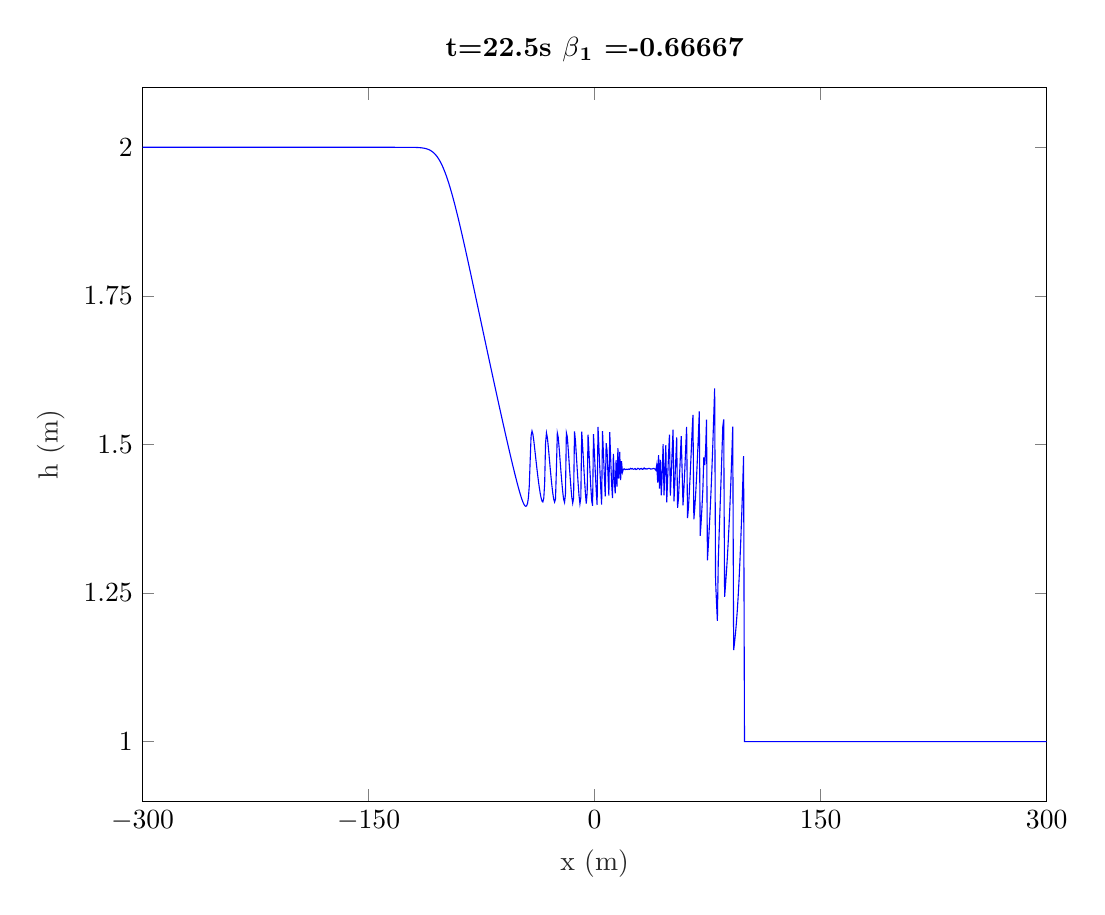
\begin{tikzpicture}

\begin{axis}[%
width=4.521in,
height=3.566in,
at={(0.758in,0.481in)},
scale only axis,
xmin=-300,
xmax=300,
xtick={-300, -150,    0,  150,  300},
xlabel style={font=\color{white!15!black}},
xlabel={x (m)},
ymin=0.9,
ymax=2.1,
ytick={   1, 1.25,  1.5, 1.75,    2},
ylabel style={font=\color{white!15!black}},
ylabel={h (m)},
axis background/.style={fill=white},
title style={font=\bfseries},
title={$\text{t=22.5s   }\beta{}_\text{1}\text{ =-0.66667}$}
]
\addplot [color=blue, forget plot]
  table[row sep=crcr]{%
-300.18000900045	2\\
-299.57997899895	2\\
-298.97994899745	2\\
-298.37991899595	2\\
-297.77988899445	2\\
-297.17985899295	2\\
-296.57982899145	2\\
-295.979798989949	2\\
-295.379768988449	2\\
-294.779738986949	2\\
-294.179708985449	2\\
-293.579678983949	2\\
-292.979648982449	2\\
-292.379618980949	2\\
-291.779588979449	2\\
-291.179558977949	2\\
-290.579528976449	2\\
-289.979498974949	2\\
-289.379468973449	2\\
-288.779438971949	2\\
-288.179408970449	2\\
-287.579378968948	2\\
-286.979348967448	2\\
-286.379318965948	2\\
-285.779288964448	2\\
-285.179258962948	2\\
-284.579228961448	2\\
-283.979198959948	2\\
-283.379168958448	2\\
-282.779138956948	2\\
-282.179108955448	2\\
-281.579078953948	2\\
-280.979048952448	2\\
-280.379018950948	2\\
-279.778988949447	2\\
-279.178958947947	2\\
-278.578928946447	2\\
-277.978898944947	2\\
-277.378868943447	2\\
-276.778838941947	2\\
-276.178808940447	2\\
-275.578778938947	2\\
-274.978748937447	2\\
-274.378718935947	2\\
-273.778688934447	2\\
-273.178658932947	2\\
-272.578628931447	2\\
-271.978598929946	2\\
-271.378568928446	2\\
-270.778538926946	2\\
-270.178508925446	2\\
-269.578478923946	2\\
-268.978448922446	2\\
-268.378418920946	2\\
-267.778388919446	2\\
-267.178358917946	2\\
-266.578328916446	2\\
-265.978298914946	2\\
-265.378268913446	2\\
-264.778238911946	2\\
-264.178208910446	2\\
-263.578178908945	2\\
-262.978148907445	2\\
-262.378118905945	2\\
-261.778088904445	2\\
-261.178058902945	2\\
-260.578028901445	2\\
-259.977998899945	2\\
-259.377968898445	2\\
-258.777938896945	2\\
-258.177908895445	2\\
-257.577878893945	2\\
-256.977848892445	2\\
-256.377818890945	2\\
-255.777788889444	2\\
-255.177758887944	2\\
-254.577728886444	2\\
-253.977698884944	2\\
-253.377668883444	2\\
-252.777638881944	2\\
-252.177608880444	2\\
-251.577578878944	2\\
-250.977548877444	2\\
-250.377518875944	2\\
-249.777488874444	2\\
-249.177458872944	2\\
-248.577428871444	2\\
-247.977398869943	2\\
-247.377368868443	2\\
-246.777338866943	2\\
-246.177308865443	2\\
-245.577278863943	2\\
-244.977248862443	2\\
-244.377218860943	2\\
-243.777188859443	2\\
-243.177158857943	2\\
-242.577128856443	2\\
-241.977098854943	2\\
-241.377068853443	2\\
-240.777038851943	2\\
-240.177008850443	2\\
-239.576978848942	2\\
-238.976948847442	2\\
-238.376918845942	2\\
-237.776888844442	2\\
-237.176858842942	2\\
-236.576828841442	2\\
-235.976798839942	2\\
-235.376768838442	2\\
-234.776738836942	2\\
-234.176708835442	2\\
-233.576678833942	2\\
-232.976648832442	2\\
-232.376618830942	2\\
-231.776588829441	2\\
-231.176558827941	2\\
-230.576528826441	2\\
-229.976498824941	2\\
-229.376468823441	2\\
-228.776438821941	2\\
-228.176408820441	2\\
-227.576378818941	2\\
-226.976348817441	2\\
-226.376318815941	2\\
-225.776288814441	2\\
-225.176258812941	2\\
-224.576228811441	2\\
-223.976198809941	2\\
-223.37616880844	2\\
-222.77613880694	2\\
-222.17610880544	2\\
-221.57607880394	2\\
-220.97604880244	2\\
-220.37601880094	2\\
-219.77598879944	2\\
-219.17595879794	2\\
-218.57592879644	2\\
-217.97589879494	2\\
-217.37586879344	2\\
-216.77583879194	2\\
-216.17580879044	2\\
-215.575778788939	2\\
-214.975748787439	2\\
-214.375718785939	2\\
-213.775688784439	2\\
-213.175658782939	2\\
-212.575628781439	2\\
-211.975598779939	2\\
-211.375568778439	2\\
-210.775538776939	2\\
-210.175508775439	2\\
-209.575478773939	2\\
-208.975448772439	2\\
-208.375418770939	2\\
-207.775388769438	2\\
-207.175358767938	2\\
-206.575328766438	2\\
-205.975298764938	2\\
-205.375268763438	2\\
-204.775238761938	2\\
-204.175208760438	2\\
-203.575178758938	2\\
-202.975148757438	2\\
-202.375118755938	2\\
-201.775088754438	2\\
-201.175058752938	2\\
-200.575028751438	2\\
-199.974998749937	2\\
-199.374968748437	2\\
-198.774938746937	2\\
-198.174908745437	2\\
-197.574878743937	2\\
-196.974848742437	2\\
-196.374818740937	2\\
-195.774788739437	2\\
-195.174758737937	2\\
-194.574728736437	2\\
-193.974698734937	2\\
-193.374668733437	2\\
-192.774638731937	2\\
-192.174608730437	2\\
-191.574578728936	2\\
-190.974548727436	2\\
-190.374518725936	2\\
-189.774488724436	2\\
-189.174458722936	2\\
-188.574428721436	2\\
-187.974398719936	2\\
-187.374368718436	2\\
-186.774338716936	2\\
-186.174308715436	2\\
-185.574278713936	2\\
-184.974248712436	2\\
-184.374218710936	2\\
-183.774188709435	2\\
-183.174158707935	2\\
-182.574128706435	2\\
-181.974098704935	2\\
-181.374068703435	2\\
-180.774038701935	2\\
-180.174008700435	2\\
-179.573978698935	2\\
-178.973948697435	2\\
-178.373918695935	2\\
-177.773888694435	2\\
-177.173858692935	2\\
-176.573828691435	2\\
-175.973798689934	2\\
-175.373768688434	2\\
-174.773738686934	2\\
-174.173708685434	2\\
-173.573678683934	2\\
-172.973648682434	2\\
-172.373618680934	2\\
-171.773588679434	2\\
-171.173558677934	2\\
-170.573528676434	2\\
-169.973498674934	2\\
-169.373468673434	2\\
-168.773438671934	2\\
-168.173408670434	2\\
-167.573378668933	2\\
-166.973348667433	2\\
-166.373318665933	1.99999999999999\\
-165.773288664433	1.99999999999997\\
-165.173258662933	1.99999999999995\\
-164.573228661433	1.99999999999992\\
-163.973198659933	1.99999999999988\\
-163.373168658433	1.99999999999983\\
-162.773138656933	1.99999999999975\\
-162.173108655433	1.99999999999965\\
-161.573078653933	1.9999999999995\\
-160.973048652433	1.99999999999931\\
-160.373018650933	1.99999999999904\\
-159.772988649432	1.99999999999867\\
-159.172958647932	1.99999999999818\\
-158.572928646432	1.99999999999749\\
-157.972898644932	1.99999999999655\\
-157.372868643432	1.99999999999525\\
-156.772838641932	1.99999999999348\\
-156.172808640432	1.99999999999108\\
-155.572778638932	1.99999999998778\\
-154.972748637432	1.99999999998331\\
-154.372718635932	1.99999999997721\\
-153.772688634432	1.99999999996891\\
-153.172658632932	1.99999999995764\\
-152.572628631432	1.99999999994236\\
-151.972598629931	1.99999999992163\\
-151.372568628431	1.99999999989357\\
-150.772538626931	1.99999999985561\\
-150.172508625431	1.99999999980433\\
-149.572478623931	1.99999999973512\\
-148.972448622431	1.99999999964183\\
-148.372418620931	1.99999999951621\\
-147.772388619431	1.99999999934728\\
-147.172358617931	1.99999999912035\\
-146.572328616431	1.9999999988159\\
-145.972298614931	1.99999999840794\\
-145.372268613431	1.99999999786195\\
-144.772238611931	1.99999999713214\\
-144.172208610431	1.99999999615787\\
-143.57217860893	1.99999999485894\\
-142.97214860743	1.99999999312943\\
-142.37211860593	1.99999999082965\\
-141.77208860443	1.99999998777568\\
-141.17205860293	1.99999998372576\\
-140.57202860143	1.99999997836251\\
-139.97199859993	1.99999997127004\\
-139.37196859843	1.9999999619042\\
-138.77193859693	1.99999994955422\\
-138.17190859543	1.99999993329327\\
-137.57187859393	1.99999991191481\\
-136.97184859243	1.99999988385101\\
-136.37181859093	1.99999984706807\\
-135.771788589429	1.9999997989326\\
-135.171758587929	1.99999973604117\\
-134.571728586429	1.99999965400344\\
-133.971698584929	1.99999954716687\\
-133.371668583429	1.99999940826823\\
-132.771638581929	1.99999922799339\\
-132.171608580429	1.99999899442277\\
-131.571578578929	1.99999869233467\\
-130.971548577429	1.99999830233226\\
-130.371518575929	1.99999779975297\\
-129.771488574429	1.99999715330973\\
-129.171458572929	1.99999632340368\\
-128.571428571429	1.99999526003516\\
-127.971398569929	1.99999390022612\\
-127.371368568428	1.9999921648505\\
-126.771338566928	1.99998995475074\\
-126.171308565428	1.99998714599734\\
-125.571278563928	1.99998358412566\\
-124.971248562428	1.99997907715812\\
-124.371218560928	1.99997338719362\\
-123.771188559428	1.99996622031707\\
-123.171158557928	1.9999572145544\\
-122.571128556428	1.99994592557114\\
-121.971098554928	1.99993180978969\\
-121.371068553428	1.99991420458315\\
-120.771038551928	1.99989230519676\\
-120.171008550428	1.99986513805475\\
-119.570978548927	1.99983153013791\\
-118.970948547427	1.99979007417049\\
-118.370918545927	1.99973908944267\\
-117.770888544427	1.99967657822456\\
-117.170858542927	1.99960017790813\\
-116.570828541427	1.99950710925227\\
-115.970798539927	1.9993941214106\\
-115.370768538427	1.99925743479343\\
-114.770738536927	1.99909268325389\\
-114.170708535427	1.99889485758409\\
-113.570678533927	1.99865825284013\\
-112.970648532427	1.99837642255564\\
-112.370618530927	1.99804214340462\\
-111.770588529426	1.99764739427895\\
-111.170558527926	1.99718335398121\\
-110.570528526426	1.99664042172179\\
-109.970498524926	1.99600826427378\\
-109.370468523426	1.9952758929166\\
-108.770438521926	1.99443177215359\\
-108.170408520426	1.99346396062867\\
-107.570378518926	1.99236028275449\\
-106.970348517426	1.99110852742431\\
-106.370318515926	1.98969666799365\\
-105.770288514426	1.98811309570803\\
-105.170258512926	1.98634685715785\\
-104.570228511426	1.98438788537296\\
-103.970198509925	1.98222721398627\\
-103.370168508425	1.97985716456035\\
-102.770138506925	1.9772714986465\\
-102.170108505425	1.9744655282871\\
-101.570078503925	1.97143618125486\\
-100.970048502425	1.96818202007616\\
-100.370018500925	1.96470321653517\\
-99.769988499425	1.9610014856616\\
-99.1699584979249	1.95707998499487\\
-98.5699284964248	1.95294318609694\\
-97.9698984949247	1.94859672584121\\
-97.3698684934247	1.94404724499019\\
-96.7698384919246	1.93930222108968\\
-96.1698084904245	1.93436980188071\\
-95.5697784889244	1.92925864439124\\
-94.9697484874244	1.92397776374062\\
-94.3697184859243	1.91853639456835\\
-93.7696884844242	1.91294386695986\\
-93.1696584829241	1.90720949783362\\
-92.5696284814241	1.90134249799961\\
-91.969598479924	1.89535189450779\\
-91.3695684784239	1.88924646746695\\
-90.7695384769239	1.88303470021533\\
-90.1695084754238	1.8767247415434\\
-89.5694784739237	1.87032437858336\\
-88.9694484724236	1.86384101896893\\
-88.3694184709235	1.85728168091176\\
-87.7693884694235	1.85065298992149\\
-87.1693584679234	1.8439611810003\\
-86.5693284664233	1.83721210525946\\
-85.9692984649232	1.83041124002619\\
-85.3692684634232	1.82356370162827\\
-84.7692384619231	1.81667426015744\\
-84.169208460423	1.80974735561836\\
-83.5691784589229	1.80278711496616\\
-82.9691484574229	1.79579736962284\\
-82.3691184559228	1.78878167313945\\
-81.7690884544227	1.78174331873992\\
-81.1690584529227	1.77468535654163\\
-80.5690284514226	1.76761061029963\\
-79.9689984499225	1.76052169356548\\
-79.3689684484224	1.75342102518882\\
-78.7689384469223	1.74631084412011\\
-78.1689084454223	1.73919322349721\\
-77.5688784439222	1.73207008401764\\
-76.9688484424221	1.72494320661182\\
-76.368818440922	1.71781424444267\\
-75.768788439422	1.7106847342637\\
-75.1687584379219	1.70355610717183\\
-74.5687284364218	1.69642969879384\\
-73.9686984349217	1.68930675894739\\
-73.3686684334217	1.68218846081898\\
-72.7686384319216	1.67507590970312\\
-72.1686084304215	1.66797015134928\\
-71.5685784289215	1.66087217996604\\
-70.9685484274214	1.65378294593583\\
-70.3685184259213	1.64670336329843\\
-69.7684884244212	1.63963431706679\\
-69.1684584229211	1.63257667044594\\
-68.5684284214211	1.62553127203351\\
-67.968398419921	1.6184989630901\\
-67.3683684184209	1.61148058497901\\
-66.7683384169208	1.60447698688883\\
-66.1683084154208	1.59748903396876\\
-65.5682784139207	1.59051761602736\\
-64.9682484124206	1.58356365697046\\
-64.3682184109205	1.57662812518562\\
-63.7681884094205	1.56971204511977\\
-63.1681584079204	1.56281651034655\\
-62.5681284064203	1.55594269848214\\
-61.9680984049203	1.54909188838869\\
-61.3680684034202	1.54226548020608\\
-60.7680384019201	1.53546501888428\\
-60.16800840042	1.52869222205837\\
-59.5679783989199	1.52194901332966\\
-58.9679483974199	1.51523756230723\\
-58.3679183959198	1.50856033314838\\
-57.7678883944197	1.50192014385014\\
-57.1678583929196	1.49532023923468\\
-56.5678283914196	1.48876438151161\\
-55.9677983899195	1.48225696359246\\
-55.3677683884194	1.47580315212916\\
-54.7677383869193	1.469409069779\\
-54.1677083854193	1.46308202980889\\
-53.5676783839192	1.45683084138178\\
-52.9676483824191	1.45066621156387\\
-52.3676183809191	1.44460128161839\\
-51.767588379419	1.43865235275257\\
-51.1675583779189	1.43283988394407\\
-50.5675283764188	1.42718988834715\\
-49.9674983749187	1.42173592678609\\
-49.3674683734187	1.41652201866562\\
-48.7674383719186	1.41160700399135\\
-48.1674083704185	1.40707127911988\\
-47.5673783689184	1.40302757160988\\
-46.9673483674184	1.39963891810045\\
-46.3673183659183	1.39715023518688\\
-45.7672883644182	1.39594747627642\\
-45.1672583629181	1.39668114367597\\
-44.5672283614181	1.40052043300619\\
-43.967198359918	1.40989044475002\\
-43.3671683584179	1.43052110298331\\
-42.7671383569178	1.47385953536934\\
-42.1671083554178	1.51446722870298\\
-41.5670783539177	1.52267451266888\\
-40.9670483524176	1.51728128267961\\
-40.3670183509175	1.50617157594423\\
-39.7669883494175	1.49289548062162\\
-39.1669583479174	1.47897215708812\\
-38.5669283464173	1.46518157131517\\
-37.9668983449172	1.45196943445554\\
-37.3668683434172	1.43962851360008\\
-36.7668383419171	1.42840329975377\\
-36.166808340417	1.4185710148083\\
-35.5667783389169	1.41053954210252\\
-34.9667483374168	1.40502041619195\\
-34.3667183359168	1.40348636661639\\
-33.7666883344167	1.40926920894489\\
-33.1666583329167	1.43426989200539\\
-32.5666283314166	1.50214331001388\\
-31.9665983299165	1.5193912635907\\
-31.3665683284164	1.51161522017108\\
-30.7665383269164	1.49659464509342\\
-30.1665083254163	1.47949714018372\\
-29.5664783239162	1.46223400364617\\
-28.9664483224161	1.44577710950126\\
-28.3664183209161	1.43077802660978\\
-27.766388319416	1.41787193742129\\
-27.1663583179159	1.40799119395956\\
-26.5663283164158	1.40312739144095\\
-25.9662983149157	1.40856496815491\\
-25.3662683134157	1.4589627438848\\
-24.7662383119156	1.5194214063987\\
-24.1662083104155	1.51192746626159\\
-23.5661783089154	1.49437933123187\\
-22.9661483074154	1.47444904182833\\
-22.3661183059153	1.45461203406818\\
-21.7660883044152	1.43614551123044\\
-21.1660583029151	1.42006939866225\\
-20.5660283014151	1.4077438755716\\
-19.965998299915	1.40247074787938\\
-19.3659682984149	1.41658260860959\\
-18.7659382969148	1.5196846053732\\
-18.1659082954148	1.51319509110438\\
-17.5658782939147	1.49330183394599\\
-16.9658482924146	1.47084365808092\\
-16.3658182909145	1.44875323178569\\
-15.7657882894144	1.42858470864017\\
-15.1657582879144	1.41185120952732\\
-14.5657282864143	1.4012288227985\\
-13.9656982849143	1.4099960164481\\
-13.3656682834142	1.52207106398172\\
-12.7656382819141	1.50739270672826\\
-12.165608280414	1.48328641922141\\
-11.565578278914	1.45817760861854\\
-10.9655482774139	1.43456848882242\\
-10.3655182759138	1.41425030202972\\
-9.76548827441371	1.40006144560171\\
-9.16545827291367	1.41064464043908\\
-8.56542827141357	1.52147120067227\\
-7.96539826991352	1.49725576109143\\
-7.36536826841342	1.46977217329494\\
-6.76533826691332	1.44293086393695\\
-6.16530826541327	1.41889676014805\\
-5.56527826391317	1.40053128904577\\
-4.96524826241313	1.41876366657493\\
-4.36521826091303	1.5166885181707\\
-3.76518825941298	1.48800087459076\\
-3.16515825791288	1.45790658673036\\
-2.56512825641283	1.42956572791536\\
-1.96509825491273	1.40563248587528\\
-1.36506825341269	1.39676684613462\\
-0.765038251912586	1.51741091059578\\
-0.165008250412541	1.48591319269781\\
0.435021751087561	1.45340934467125\\
1.03505175258761	1.42300353963462\\
1.63508175408771	1.39820355415017\\
2.23511175558775	1.52938039916067\\
2.83514175708785	1.49514826278827\\
3.43517175858796	1.46012637041103\\
4.035201760088	1.42691062554491\\
4.6352317615881	1.39879955735154\\
5.23526176308815	1.52263205159782\\
5.83529176458825	1.48436874892975\\
6.43532176608829	1.44703356776706\\
7.03535176758839	1.41284730223141\\
7.63538176908844	1.50226159316499\\
8.23541177058854	1.48993756058028\\
8.83544177208859	1.45062020709289\\
9.43547177358869	1.41403395159715\\
10.0355017750887	1.52055042156894\\
10.6355317765888	1.47622701789432\\
11.2355617780889	1.43506911711145\\
11.835591779589	1.40993189625035\\
12.435621781089	1.48416445327547\\
13.0356517825891	1.44088027923167\\
13.6356817840892	1.41775243572858\\
14.2357117855893	1.47361475438135\\
14.8357417870894	1.42902848860641\\
15.4357717885894	1.49363328806839\\
16.0358017900895	1.44273087254956\\
16.6358317915896	1.48759130458428\\
17.2358617930897	1.44000273702405\\
17.8358917945897	1.47192760543845\\
18.4359217960898	1.4530644418659\\
19.0359517975899	1.45814503358371\\
19.63598179909	1.45908548664713\\
20.23601180059	1.45768898217982\\
20.8360418020901	1.45801792694949\\
21.4360718035902	1.45844807550219\\
22.0361018050903	1.45787437053238\\
22.6361318065904	1.45870413658682\\
23.2361618080904	1.45820680358124\\
23.8361918095905	1.45981997255124\\
24.4362218110905	1.45880432132111\\
25.0362518125906	1.45951731110036\\
25.6362818140907	1.45834430409111\\
26.2363118155908	1.45859982275159\\
26.8363418170908	1.45952040526712\\
27.4363718185909	1.45776204115595\\
28.036401820091	1.45839179535419\\
28.6364318215911	1.45993239699658\\
29.2364618230911	1.45954599792161\\
29.8364918245912	1.45803741377468\\
30.4365218260913	1.45931145599716\\
31.0365518275914	1.45969651219426\\
31.6365818290914	1.45817476100281\\
32.2366118305915	1.45858919993897\\
32.8366418320916	1.46052475384374\\
33.4366718335917	1.45871916698221\\
34.0367018350918	1.45928550594765\\
34.6367318365918	1.45853693855822\\
35.2367618380919	1.45923358882711\\
35.836791839592	1.45973702268318\\
36.4368218410921	1.45968013487477\\
37.0368518425921	1.45871310049995\\
37.6368818440922	1.45880177781426\\
38.2369118455923	1.458951105919\\
38.8369418470924	1.45955710945907\\
39.4369718485924	1.45963516048476\\
40.0370018500925	1.45853210494956\\
40.6370318515926	1.45650624952145\\
41.2370618530927	1.46572951671608\\
41.8370918545928	1.43577911087661\\
42.4371218560928	1.48219120433283\\
43.0371518575929	1.42594467982756\\
43.6371818590929	1.47406460280048\\
44.237211860593	1.41432107964452\\
44.8372418620931	1.45263299901259\\
45.4372718635932	1.50037223054468\\
46.0373018650932	1.41458445237987\\
46.6373318665933	1.45675996913429\\
47.2373618680934	1.49900341400457\\
47.8373918695935	1.40274201979605\\
48.4374218710935	1.44211754122049\\
49.0374518725936	1.48260446038323\\
49.6374818740937	1.51646653429021\\
50.2375118755938	1.41394872452946\\
50.8375418770938	1.44947860191484\\
51.4375718785939	1.48838539167115\\
52.037601880094	1.52496204319674\\
52.6376318815941	1.4044317129554\\
53.2376618830942	1.43696696301843\\
53.8376918845942	1.47364769438764\\
54.4377218860943	1.51187217431626\\
55.0377518875944	1.39347301314351\\
55.6377818890945	1.40971279679381\\
56.2378118905945	1.44162816928717\\
56.8378418920946	1.4771225636943\\
57.4378718935947	1.51392517898079\\
58.0379018950948	1.45728913364979\\
58.6379318965948	1.39740729910233\\
59.2379618980949	1.42557494178883\\
59.837991899595	1.45837461687284\\
60.4380219010951	1.49585801129615\\
61.0380519025952	1.52958261487633\\
61.6380819040952	1.3759694859715\\
62.2381119055953	1.3931088607277\\
62.8381419070953	1.41968134406528\\
63.4381719085955	1.45066467360745\\
64.0382019100955	1.48464878847612\\
64.6382319115956	1.52036443098615\\
65.2382619130956	1.54988845035001\\
65.8382919145957	1.37396221603241\\
66.4383219160958	1.39253639221856\\
67.0383519175959	1.41672265557231\\
67.6383819190959	1.44515740233133\\
68.238411920596	1.47860260024973\\
68.8384419220961	1.5155303497308\\
69.4384719235962	1.55549675966779\\
70.0385019250962	1.34630652450734\\
70.6385319265963	1.36778227904351\\
71.2385619280964	1.39484756899449\\
71.8385919295965	1.4263179553342\\
72.4386219310966	1.47835947471173\\
73.0386519325966	1.46545607667308\\
73.6386819340967	1.49042324674457\\
74.2387119355968	1.54187299624993\\
74.8387419370969	1.30508062154299\\
75.4387719385969	1.32983955572813\\
76.038801940097	1.3574433607451\\
76.6388319415971	1.3880519282928\\
77.2388619430972	1.42192283771036\\
77.8388919445972	1.4597340161925\\
78.4389219460973	1.5011642207113\\
79.0389519475974	1.54777580272018\\
79.6389819490975	1.59431090979504\\
80.2390119505975	1.2724009792474\\
80.8390419520976	1.23523574066804\\
81.4390719535977	1.20328154387485\\
82.0391019550977	1.30290665189129\\
82.6391319565979	1.35184417025365\\
83.2391619580979	1.39461177521534\\
83.839191959598	1.43758240667516\\
84.439221961098	1.48247157110071\\
85.0392519625981	1.52983503981811\\
85.6392819640982	1.5420678774349\\
86.2393119655983	1.24347598737264\\
86.8393419670983	1.26288757045844\\
87.4393719685984	1.28441538170838\\
88.0394019700985	1.30857044869884\\
88.6394319715986	1.33586077400031\\
89.2394619730986	1.36673748998682\\
89.8394919745987	1.40158655310174\\
90.4395219760988	1.4403142191926\\
91.0395519775989	1.48322062009017\\
91.639581979099	1.53002853679684\\
92.239611980599	1.15386482036444\\
92.8396419820991	1.1667518473746\\
93.4396719835992	1.18165486285686\\
94.0397019850993	1.19911736634628\\
94.6397319865993	1.2198142994923\\
95.2397619880994	1.24419919831694\\
95.8397919895995	1.27267211302838\\
96.4398219910996	1.30558711628585\\
97.0398519925996	1.34301207316073\\
97.6398819940997	1.38469587269072\\
98.2399119955998	1.43061707599231\\
98.8399419970999	1.48054585559873\\
99.4399719985999	1.00000001955143\\
100.0400020001	1.00000000859405\\
100.6400320016	1.00000000395353\\
101.2400620031	1.00000000184846\\
101.8400920046	1.000000000875\\
102.4401220061	1.00000000041819\\
103.0401520076	1.00000000020137\\
103.6401820091	1.00000000009755\\
104.240212010601	1.00000000004748\\
104.840242012101	1.00000000002319\\
105.440272013601	1.00000000001137\\
106.040302015101	1.00000000000558\\
106.640332016601	1.00000000000274\\
107.240362018101	1.00000000000134\\
107.840392019601	1.00000000000065\\
108.440422021101	1.00000000000033\\
109.040452022601	1.00000000000016\\
109.640482024101	1.00000000000008\\
110.240512025601	1.00000000000002\\
110.840542027101	1\\
111.440572028601	1\\
112.040602030102	1\\
112.640632031602	1\\
113.240662033102	1\\
113.840692034602	1\\
114.440722036102	1\\
115.040752037602	1\\
115.640782039102	1\\
116.240812040602	1\\
116.840842042102	1\\
117.440872043602	1\\
118.040902045102	1\\
118.640932046602	1\\
119.240962048102	1\\
119.840992049603	1\\
120.441022051103	1\\
121.041052052603	1\\
121.641082054103	1\\
122.241112055603	1\\
122.841142057103	1\\
123.441172058603	1\\
124.041202060103	1\\
124.641232061603	1\\
125.241262063103	1\\
125.841292064603	1\\
126.441322066103	1\\
127.041352067603	1\\
127.641382069103	1\\
128.241412070604	1\\
128.841442072104	1\\
129.441472073604	1\\
130.041502075104	1\\
130.641532076604	1\\
131.241562078104	1\\
131.841592079604	1\\
132.441622081104	1\\
133.041652082604	1\\
133.641682084104	1\\
134.241712085604	1\\
134.841742087104	1\\
135.441772088604	1\\
136.041802090105	1\\
136.641832091605	1\\
137.241862093105	1\\
137.841892094605	1\\
138.441922096105	1\\
139.041952097605	1\\
139.641982099105	1\\
140.242012100605	1\\
140.842042102105	1\\
141.442072103605	1\\
142.042102105105	1\\
142.642132106605	1\\
143.242162108105	1\\
143.842192109605	1\\
144.442222111106	1\\
145.042252112606	1\\
145.642282114106	1\\
146.242312115606	1\\
146.842342117106	1\\
147.442372118606	1\\
148.042402120106	1\\
148.642432121606	1\\
149.242462123106	1\\
149.842492124606	1\\
150.442522126106	1\\
151.042552127606	1\\
151.642582129106	1\\
152.242612130607	1\\
152.842642132107	1\\
153.442672133607	1\\
154.042702135107	1\\
154.642732136607	1\\
155.242762138107	1\\
155.842792139607	1\\
156.442822141107	1\\
157.042852142607	1\\
157.642882144107	1\\
158.242912145607	1\\
158.842942147107	1\\
159.442972148607	1\\
160.043002150107	1\\
160.643032151608	1\\
161.243062153108	1\\
161.843092154608	1\\
162.443122156108	1\\
163.043152157608	1\\
163.643182159108	1\\
164.243212160608	1\\
164.843242162108	1\\
165.443272163608	1\\
166.043302165108	1\\
166.643332166608	1\\
167.243362168108	1\\
167.843392169608	1\\
168.443422171109	1\\
169.043452172609	1\\
169.643482174109	1\\
170.243512175609	1\\
170.843542177109	1\\
171.443572178609	1\\
172.043602180109	1\\
172.643632181609	1\\
173.243662183109	1\\
173.843692184609	1\\
174.443722186109	1\\
175.043752187609	1\\
175.643782189109	1\\
176.24381219061	1\\
176.84384219211	1\\
177.44387219361	1\\
178.04390219511	1\\
178.64393219661	1\\
179.24396219811	1\\
179.84399219961	1\\
180.44402220111	1\\
181.04405220261	1\\
181.64408220411	1\\
182.24411220561	1\\
182.84414220711	1\\
183.44417220861	1\\
184.04420221011	1\\
184.644232211611	1\\
185.244262213111	1\\
185.844292214611	1\\
186.444322216111	1\\
187.044352217611	1\\
187.644382219111	1\\
188.244412220611	1\\
188.844442222111	1\\
189.444472223611	1\\
190.044502225111	1\\
190.644532226611	1\\
191.244562228111	1\\
191.844592229611	1\\
192.444622231112	1\\
193.044652232612	1\\
193.644682234112	1\\
194.244712235612	1\\
194.844742237112	1\\
195.444772238612	1\\
196.044802240112	1\\
196.644832241612	1\\
197.244862243112	1\\
197.844892244612	1\\
198.444922246112	1\\
199.044952247612	1\\
199.644982249112	1\\
200.245012250613	1\\
200.845042252113	1\\
201.445072253613	1\\
202.045102255113	1\\
202.645132256613	1\\
203.245162258113	1\\
203.845192259613	1\\
204.445222261113	1\\
205.045252262613	1\\
205.645282264113	1\\
206.245312265613	1\\
206.845342267113	1\\
207.445372268613	1\\
208.045402270114	1\\
208.645432271614	1\\
209.245462273114	1\\
209.845492274614	1\\
210.445522276114	1\\
211.045552277614	1\\
211.645582279114	1\\
212.245612280614	1\\
212.845642282114	1\\
213.445672283614	1\\
214.045702285114	1\\
214.645732286614	1\\
215.245762288114	1\\
215.845792289614	1\\
216.445822291115	1\\
217.045852292615	1\\
217.645882294115	1\\
218.245912295615	1\\
218.845942297115	1\\
219.445972298615	1\\
220.046002300115	1\\
220.646032301615	1\\
221.246062303115	1\\
221.846092304615	1\\
222.446122306115	1\\
223.046152307615	1\\
223.646182309115	1\\
224.246212310616	1\\
224.846242312116	1\\
225.446272313616	1\\
226.046302315116	1\\
226.646332316616	1\\
227.246362318116	1\\
227.846392319616	1\\
228.446422321116	1\\
229.046452322616	1\\
229.646482324116	1\\
230.246512325616	1\\
230.846542327116	1\\
231.446572328616	1\\
232.046602330116	1\\
232.646632331617	1\\
233.246662333117	1\\
233.846692334617	1\\
234.446722336117	1\\
235.046752337617	1\\
235.646782339117	1\\
236.246812340617	1\\
236.846842342117	1\\
237.446872343617	1\\
238.046902345117	1\\
238.646932346617	1\\
239.246962348117	1\\
239.846992349617	1\\
240.447022351118	1\\
241.047052352618	1\\
241.647082354118	1\\
242.247112355618	1\\
242.847142357118	1\\
243.447172358618	1\\
244.047202360118	1\\
244.647232361618	1\\
245.247262363118	1\\
245.847292364618	1\\
246.447322366118	1\\
247.047352367618	1\\
247.647382369118	1\\
248.247412370619	1\\
248.847442372119	1\\
249.447472373619	1\\
250.047502375119	1\\
250.647532376619	1\\
251.247562378119	1\\
251.847592379619	1\\
252.447622381119	1\\
253.047652382619	1\\
253.647682384119	1\\
254.247712385619	1\\
254.847742387119	1\\
255.447772388619	1\\
256.04780239012	1\\
256.64783239162	1\\
257.24786239312	1\\
257.84789239462	1\\
258.44792239612	1\\
259.04795239762	1\\
259.64798239912	1\\
260.24801240062	1\\
260.84804240212	1\\
261.44807240362	1\\
262.04810240512	1\\
262.64813240662	1\\
263.24816240812	1\\
263.84819240962	1\\
264.448222411121	1\\
265.048252412621	1\\
265.648282414121	1\\
266.248312415621	1\\
266.848342417121	1\\
267.448372418621	1\\
268.048402420121	1\\
268.648432421621	1\\
269.248462423121	1\\
269.848492424621	1\\
270.448522426121	1\\
271.048552427621	1\\
271.648582429121	1\\
272.248612430622	1\\
272.848642432122	1\\
273.448672433622	1\\
274.048702435122	1\\
274.648732436622	1\\
275.248762438122	1\\
275.848792439622	1\\
276.448822441122	1\\
277.048852442622	1\\
277.648882444122	1\\
278.248912445622	1\\
278.848942447122	1\\
279.448972448622	1\\
280.049002450123	1\\
280.649032451623	1\\
281.249062453123	1\\
281.849092454623	1\\
282.449122456123	1\\
283.049152457623	1\\
283.649182459123	1\\
284.249212460623	1\\
284.849242462123	1\\
285.449272463623	1\\
286.049302465123	1\\
286.649332466623	1\\
287.249362468123	1\\
287.849392469623	1\\
288.449422471124	1\\
289.049452472624	1\\
289.649482474124	1\\
290.249512475624	1\\
290.849542477124	1\\
291.449572478624	1\\
292.049602480124	1\\
292.649632481624	1\\
293.249662483124	1\\
293.849692484624	1\\
294.449722486124	1\\
295.049752487624	1\\
295.649782489125	1\\
296.249812490625	1\\
296.849842492125	1\\
297.449872493625	1\\
298.049902495125	1\\
298.649932496625	1\\
299.249962498125	1\\
299.849992499625	1\\
};
\end{axis}
\end{tikzpicture}%
		\caption{$t=22.5s$}
	\end{subfigure}
	\begin{subfigure}{0.49\textwidth}
		\centering
		% This file was created by matlab2tikz.
%
%The latest updates can be retrieved from
%  http://www.mathworks.com/matlabcentral/fileexchange/22022-matlab2tikz-matlab2tikz
%where you can also make suggestions and rate matlab2tikz.
%
\begin{tikzpicture}

\begin{axis}[%
width=4.521in,
height=3.566in,
at={(0.758in,0.481in)},
scale only axis,
xmin=-300,
xmax=300,
xtick={-300, -150,    0,  150,  300},
xlabel style={font=\color{white!15!black}},
xlabel={x (m)},
ymin=0.9,
ymax=2.1,
ytick={   1, 1.25,  1.5, 1.75,    2},
ylabel style={font=\color{white!15!black}},
ylabel={h (m)},
axis background/.style={fill=white},
title style={font=\bfseries},
title={$\text{t=25s   }\beta{}_\text{1}\text{ =-0.66667}$}
]
\addplot [color=blue, forget plot]
  table[row sep=crcr]{%
-300.18000900045	2\\
-299.57997899895	2\\
-298.97994899745	2\\
-298.37991899595	2\\
-297.77988899445	2\\
-297.17985899295	2\\
-296.57982899145	2\\
-295.979798989949	2\\
-295.379768988449	2\\
-294.779738986949	2\\
-294.179708985449	2\\
-293.579678983949	2\\
-292.979648982449	2\\
-292.379618980949	2\\
-291.779588979449	2\\
-291.179558977949	2\\
-290.579528976449	2\\
-289.979498974949	2\\
-289.379468973449	2\\
-288.779438971949	2\\
-288.179408970449	2\\
-287.579378968948	2\\
-286.979348967448	2\\
-286.379318965948	2\\
-285.779288964448	2\\
-285.179258962948	2\\
-284.579228961448	2\\
-283.979198959948	2\\
-283.379168958448	2\\
-282.779138956948	2\\
-282.179108955448	2\\
-281.579078953948	2\\
-280.979048952448	2\\
-280.379018950948	2\\
-279.778988949447	2\\
-279.178958947947	2\\
-278.578928946447	2\\
-277.978898944947	2\\
-277.378868943447	2\\
-276.778838941947	2\\
-276.178808940447	2\\
-275.578778938947	2\\
-274.978748937447	2\\
-274.378718935947	2\\
-273.778688934447	2\\
-273.178658932947	2\\
-272.578628931447	2\\
-271.978598929946	2\\
-271.378568928446	2\\
-270.778538926946	2\\
-270.178508925446	2\\
-269.578478923946	2\\
-268.978448922446	2\\
-268.378418920946	2\\
-267.778388919446	2\\
-267.178358917946	2\\
-266.578328916446	2\\
-265.978298914946	2\\
-265.378268913446	2\\
-264.778238911946	2\\
-264.178208910446	2\\
-263.578178908945	2\\
-262.978148907445	2\\
-262.378118905945	2\\
-261.778088904445	2\\
-261.178058902945	2\\
-260.578028901445	2\\
-259.977998899945	2\\
-259.377968898445	2\\
-258.777938896945	2\\
-258.177908895445	2\\
-257.577878893945	2\\
-256.977848892445	2\\
-256.377818890945	2\\
-255.777788889444	2\\
-255.177758887944	2\\
-254.577728886444	2\\
-253.977698884944	2\\
-253.377668883444	2\\
-252.777638881944	2\\
-252.177608880444	2\\
-251.577578878944	2\\
-250.977548877444	2\\
-250.377518875944	2\\
-249.777488874444	2\\
-249.177458872944	2\\
-248.577428871444	2\\
-247.977398869943	2\\
-247.377368868443	2\\
-246.777338866943	2\\
-246.177308865443	2\\
-245.577278863943	2\\
-244.977248862443	2\\
-244.377218860943	2\\
-243.777188859443	2\\
-243.177158857943	2\\
-242.577128856443	2\\
-241.977098854943	2\\
-241.377068853443	2\\
-240.777038851943	2\\
-240.177008850443	2\\
-239.576978848942	2\\
-238.976948847442	2\\
-238.376918845942	2\\
-237.776888844442	2\\
-237.176858842942	2\\
-236.576828841442	2\\
-235.976798839942	2\\
-235.376768838442	2\\
-234.776738836942	2\\
-234.176708835442	2\\
-233.576678833942	2\\
-232.976648832442	2\\
-232.376618830942	2\\
-231.776588829441	2\\
-231.176558827941	2\\
-230.576528826441	2\\
-229.976498824941	2\\
-229.376468823441	2\\
-228.776438821941	2\\
-228.176408820441	2\\
-227.576378818941	2\\
-226.976348817441	2\\
-226.376318815941	2\\
-225.776288814441	2\\
-225.176258812941	2\\
-224.576228811441	2\\
-223.976198809941	2\\
-223.37616880844	2\\
-222.77613880694	2\\
-222.17610880544	2\\
-221.57607880394	2\\
-220.97604880244	2\\
-220.37601880094	2\\
-219.77598879944	2\\
-219.17595879794	2\\
-218.57592879644	2\\
-217.97589879494	2\\
-217.37586879344	2\\
-216.77583879194	2\\
-216.17580879044	2\\
-215.575778788939	2\\
-214.975748787439	2\\
-214.375718785939	2\\
-213.775688784439	2\\
-213.175658782939	2\\
-212.575628781439	2\\
-211.975598779939	2\\
-211.375568778439	2\\
-210.775538776939	2\\
-210.175508775439	2\\
-209.575478773939	2\\
-208.975448772439	2\\
-208.375418770939	2\\
-207.775388769438	2\\
-207.175358767938	2\\
-206.575328766438	2\\
-205.975298764938	2\\
-205.375268763438	2\\
-204.775238761938	2\\
-204.175208760438	2\\
-203.575178758938	2\\
-202.975148757438	2\\
-202.375118755938	2\\
-201.775088754438	2\\
-201.175058752938	2\\
-200.575028751438	2\\
-199.974998749937	2\\
-199.374968748437	2\\
-198.774938746937	2\\
-198.174908745437	2\\
-197.574878743937	2\\
-196.974848742437	2\\
-196.374818740937	2\\
-195.774788739437	2\\
-195.174758737937	2\\
-194.574728736437	2\\
-193.974698734937	2\\
-193.374668733437	2\\
-192.774638731937	2\\
-192.174608730437	2\\
-191.574578728936	2\\
-190.974548727436	2\\
-190.374518725936	2\\
-189.774488724436	2\\
-189.174458722936	2\\
-188.574428721436	2\\
-187.974398719936	2\\
-187.374368718436	2\\
-186.774338716936	2\\
-186.174308715436	2\\
-185.574278713936	2\\
-184.974248712436	2\\
-184.374218710936	2\\
-183.774188709435	2\\
-183.174158707935	2\\
-182.574128706435	2\\
-181.974098704935	2\\
-181.374068703435	2\\
-180.774038701935	2\\
-180.174008700435	2\\
-179.573978698935	2\\
-178.973948697435	2\\
-178.373918695935	2\\
-177.773888694435	1.99999999999999\\
-177.173858692935	1.99999999999998\\
-176.573828691435	1.99999999999996\\
-175.973798689934	1.99999999999993\\
-175.373768688434	1.99999999999989\\
-174.773738686934	1.99999999999984\\
-174.173708685434	1.99999999999977\\
-173.573678683934	1.99999999999967\\
-172.973648682434	1.99999999999954\\
-172.373618680934	1.99999999999936\\
-171.773588679434	1.99999999999911\\
-171.173558677934	1.99999999999878\\
-170.573528676434	1.99999999999832\\
-169.973498674934	1.99999999999768\\
-169.373468673434	1.99999999999681\\
-168.773438671934	1.99999999999561\\
-168.173408670434	1.99999999999398\\
-167.573378668933	1.99999999999175\\
-166.973348667433	1.99999999998871\\
-166.373318665933	1.99999999998456\\
-165.773288664433	1.99999999997891\\
-165.173258662933	1.99999999997123\\
-164.573228661433	1.99999999996079\\
-163.973198659933	1.99999999994663\\
-163.373168658433	1.99999999992742\\
-162.773138656933	1.9999999999014\\
-162.173108655433	1.9999999998662\\
-161.573078653933	1.99999999981863\\
-160.973048652433	1.99999999975441\\
-160.373018650933	1.99999999966782\\
-159.772988649432	1.99999999955119\\
-159.172958647932	1.9999999993943\\
-158.572928646432	1.99999999918349\\
-157.972898644932	1.99999999890058\\
-157.372868643432	1.99999999852136\\
-156.772838641932	1.99999999801367\\
-156.172808640432	1.99999999733485\\
-155.572778638932	1.99999999642836\\
-154.972748637432	1.9999999952194\\
-154.372718635932	1.99999999360915\\
-153.772688634432	1.99999999146725\\
-153.172658632932	1.99999998862198\\
-152.572628631432	1.99999998484751\\
-151.972598629931	1.99999997984729\\
-151.372568628431	1.99999997323256\\
-150.772538626931	1.99999996449445\\
-150.172508625431	1.99999995296801\\
-149.572478623931	1.99999993778577\\
-148.972448622431	1.99999991781801\\
-148.372418620931	1.99999989159602\\
-147.772388619431	1.9999998572138\\
-147.172358617931	1.99999981220225\\
-146.572328616431	1.99999975336881\\
-145.972298614931	1.9999996765932\\
-145.372268613431	1.99999957656799\\
-144.772238611931	1.99999944647006\\
-144.172208610431	1.99999927754522\\
-143.57217860893	1.99999905858473\\
-142.97214860743	1.99999877526707\\
-142.37211860593	1.99999840933279\\
-141.77208860443	1.99999793755268\\
-141.17205860293	1.99999733044164\\
-140.57202860143	1.99999655066016\\
-139.97199859993	1.99999555103395\\
-139.37196859843	1.99999427210852\\
-138.77193859693	1.99999263913972\\
-138.17190859543	1.99999055840377\\
-137.57187859393	1.99998791268946\\
-136.97184859243	1.99998455581353\\
-136.37181859093	1.99998030597518\\
-135.771788589429	1.99997493773989\\
-135.171758587929	1.99996817241546\\
-134.571728586429	1.99995966655595\\
-133.971698584929	1.99994899830414\\
-133.371668583429	1.99993565126061\\
-132.771638581929	1.999918995553\\
-132.171608580429	1.99989826577329\\
-131.571578578929	1.99987253546148\\
-130.971548577429	1.99984068784445\\
-130.371518575929	1.99980138259763\\
-129.771488574429	1.99975301849115\\
-129.171458572929	1.99969369192095\\
-128.571428571429	1.99962115151699\\
-127.971398569929	1.99953274927437\\
-127.371368568428	1.99942538897362\\
-126.771338566928	1.99929547304758\\
-126.171308565428	1.99913884950862\\
-125.571278563928	1.99895076105998\\
-124.971248562428	1.99872579905313\\
-124.371218560928	1.99845786548117\\
-123.771188559428	1.9981401466608\\
-123.171158557928	1.99776510258387\\
-122.571128556428	1.99732447603162\\
-121.971098554928	1.99680932535665\\
-121.371068553428	1.99621008427271\\
-120.771038551928	1.99551665099952\\
-120.171008550428	1.99471850767833\\
-119.570978548927	1.99380486915416\\
-118.970948547427	1.99276485812672\\
-118.370918545927	1.99158770148953\\
-117.770888544427	1.99026294063637\\
-117.170858542927	1.98878064687188\\
-116.570828541427	1.98713163205127\\
-115.970798539927	1.98530764436147\\
-115.370768538427	1.98330153981371\\
-114.770738536927	1.98110742149607\\
-114.170708535427	1.9787207407735\\
-113.570678533927	1.97613835717417\\
-112.970648532427	1.9733585563759\\
-112.370618530927	1.97038102822024\\
-111.770588529426	1.96720680880039\\
-111.170558527926	1.96383819223702\\
-110.570528526426	1.96027861870429\\
-109.970498524926	1.95653254561336\\
-109.370468523426	1.95260530868022\\
-108.770438521926	1.94850297901754\\
-108.170408520426	1.94423222152978\\
-107.570378518926	1.93980015888529\\
-106.970348517426	1.93521424429861\\
-106.370318515926	1.93048214536359\\
-105.770288514426	1.92561164029173\\
-105.170258512926	1.92061052716028\\
-104.570228511426	1.9154865461739\\
-103.970198509925	1.91024731448854\\
-103.370168508425	1.90490027282283\\
-102.770138506925	1.89945264287336\\
-102.170108505425	1.89391139443408\\
-101.570078503925	1.88828322107722\\
-100.970048502425	1.88257452326433\\
-100.370018500925	1.87679139780651\\
-99.769988499425	1.87093963266762\\
-99.1699584979249	1.86502470619477\\
-98.5699284964248	1.859051789957\\
-97.9698984949247	1.85302575447129\\
-97.3698684934247	1.84695117718963\\
-96.7698384919246	1.84083235221027\\
-96.1698084904245	1.83467330125768\\
-95.5697784889244	1.82847778554988\\
-94.9697484874244	1.82224931823673\\
-94.3697184859243	1.81599117714997\\
-93.7696884844242	1.80970641765567\\
-93.1696584829241	1.80339788544133\\
-92.5696284814241	1.79706822910671\\
-91.969598479924	1.79071991245715\\
-91.3695684784239	1.7843552264233\\
-90.7695384769239	1.77797630055278\\
-90.1695084754238	1.77158511403553\\
-89.5694784739237	1.76518350623944\\
-88.9694484724236	1.75877318674359\\
-88.3694184709235	1.75235574486604\\
-87.7693884694235	1.74593265868988\\
-87.1693584679234	1.73950530359747\\
-86.5693284664233	1.73307496032694\\
-85.9692984649232	1.7266428225688\\
-85.3692684634232	1.72021000412319\\
-84.7692384619231	1.71377754564039\\
-84.169208460423	1.70734642096903\\
-83.5691784589229	1.70091754313772\\
-82.9691484574229	1.69449176999691\\
-82.3691184559228	1.68806990954891\\
-81.7690884544227	1.6816527249947\\
-81.1690584529227	1.67524093952729\\
-80.5690284514226	1.66883524090201\\
-79.9689984499225	1.6624362858152\\
-79.3689684484224	1.6560447041239\\
-78.7689384469223	1.6496611029401\\
-78.1689084454223	1.64328607063451\\
-77.5688784439222	1.63692018078633\\
-76.9688484424221	1.63056399611719\\
-76.368818440922	1.62421807244936\\
-75.768788439422	1.61788296273111\\
-75.1687584379219	1.61155922117481\\
-74.5687284364218	1.60524740755773\\
-73.9686984349217	1.59894809174038\\
-73.3686684334217	1.592661858464\\
-72.7686384319216	1.58638931249799\\
-72.1686084304215	1.58013108421915\\
-71.5685784289215	1.57388783572022\\
-70.9685484274214	1.56766026756429\\
-70.3685184259213	1.56144912632666\\
-69.7684884244212	1.55525521309687\\
-69.1684584229211	1.54907939315332\\
-68.5684284214211	1.54292260707179\\
-67.968398419921	1.53678588359138\\
-67.3683684184209	1.53067035463812\\
-66.7683384169208	1.52457727300475\\
-66.1683084154208	1.51850803330905\\
-65.5682784139207	1.51246419701261\\
-64.9682484124206	1.50644752248941\\
-64.3682184109205	1.5004600014056\\
-63.7681884094205	1.49450390303271\\
-63.1681584079204	1.4885818286018\\
-62.5681284064203	1.4826967784634\\
-61.9680984049203	1.47685223572066\\
-61.3680684034202	1.47105227125762\\
-60.7680384019201	1.46530167684848\\
-60.16800840042	1.45960613555268\\
-59.5679783989199	1.45397244225149\\
-58.9679483974199	1.44840879256632\\
-58.3679183959198	1.44292516649385\\
-57.7678883944197	1.4375338455242\\
-57.1678583929196	1.43225012156291\\
-56.5678283914196	1.42709328758115\\
-55.9677983899195	1.42208805259668\\
-55.3677683884194	1.4172666145667\\
-54.7677383869193	1.41267178852272\\
-54.1677083854193	1.40836189669704\\
-53.5676783839192	1.40441874714612\\
-52.9676483824191	1.4009613602459\\
-52.3676183809191	1.39817123495332\\
-51.767588379419	1.39633659403595\\
-51.1675583779189	1.39600859986692\\
-50.5675283764188	1.398221369887\\
-49.9674983749187	1.40586282940103\\
-49.3674683734187	1.43657927439677\\
-48.7674383719186	1.52230317787172\\
-48.1674083704185	1.52094118201505\\
-47.5673783689184	1.51297654521283\\
-46.9673483674184	1.50282642228121\\
-46.3673183659183	1.49176600946715\\
-45.7672883644182	1.48041394681264\\
-45.1672583629181	1.46911383836364\\
-44.5672283614181	1.45808119169003\\
-43.967198359918	1.44747083944869\\
-43.3671683584179	1.43741421308739\\
-42.7671383569178	1.42804929973955\\
-42.1671083554178	1.41955382752425\\
-41.5670783539177	1.41220041496023\\
-40.9670483524176	1.40647593787909\\
-40.3670183509175	1.40345872386922\\
-39.7669883494175	1.406107625371\\
-39.1669583479174	1.51750081758579\\
-38.5669283464173	1.51740324283407\\
-37.9668983449172	1.50707844410019\\
-37.3668683434172	1.49448140768315\\
-36.7668383419171	1.48108388073485\\
-36.166808340417	1.46757811638677\\
-35.5667783389169	1.45435577618803\\
-34.9667483374168	1.44169819382546\\
-34.3667183359168	1.42986928986202\\
-33.7666883344167	1.4191947196533\\
-33.1666583329167	1.41020664546424\\
-32.5666283314166	1.40392098995977\\
-31.9665983299165	1.40461623639784\\
-31.3665683284164	1.5181598122697\\
-30.7665383269164	1.50662107249067\\
-30.1665083254163	1.49241127486809\\
-29.5664783239162	1.47737464689214\\
-28.9664483224161	1.46231926031519\\
-28.3664183209161	1.44769706673497\\
-27.766388319416	1.43386815085646\\
-27.1663583179159	1.42124221143221\\
-26.5663283164158	1.4104863367189\\
-25.9662983149157	1.40290650309123\\
-25.3662683134157	1.51865874415437\\
-24.7662383119156	1.5070949722863\\
-24.1662083104155	1.49153526816991\\
-23.5661783089154	1.4750951320759\\
-22.9661483074154	1.45869007903176\\
-22.3661183059153	1.44282046350311\\
-21.7660883044152	1.42792151768366\\
-21.1660583029151	1.41458993134666\\
-20.5660283014151	1.40401089918828\\
-19.965998299915	1.51810439000087\\
-19.3659682984149	1.50172357623184\\
-18.7659382969148	1.48423066981147\\
-18.1659082954148	1.46641792901031\\
-17.5658782939147	1.44893809715146\\
-16.9658482924146	1.43227672451863\\
-16.3658182909145	1.41701350348682\\
-15.7657882894144	1.40413552381311\\
-15.1657582879144	1.51298333214241\\
-14.5657282864143	1.49398425244849\\
-13.9656982849143	1.47495599748979\\
-13.3656682834142	1.45604751552883\\
-12.7656382819141	1.43777674165589\\
-12.165608280414	1.42067935392999\\
-11.565578278914	1.40539034901675\\
-10.9655482774139	1.50721333198693\\
-10.3655182759138	1.48770905806678\\
-9.76548827441371	1.46744059531822\\
-9.16545827291367	1.44749853066086\\
-8.56542827141357	1.42842060244016\\
-7.96539826991352	1.41090808383329\\
-7.36536826841342	1.5087855974718\\
-6.76533826691332	1.48595267778435\\
-6.16530826541327	1.46462812561284\\
-5.56527826391317	1.44376894249348\\
-4.96524826241313	1.42383512533527\\
-4.36521826091303	1.41331806125029\\
-3.76518825941298	1.49238154091063\\
-3.16515825791288	1.46971370387149\\
-2.56512825641283	1.44774520090983\\
-1.96509825491273	1.42657958017912\\
-1.36506825341269	1.43311761996868\\
-0.765038251912586	1.48541089836831\\
-0.165008250412541	1.46194812954698\\
0.435021751087561	1.43917017283605\\
1.03505175258761	1.41677300084167\\
1.63508175408771	1.48767983377922\\
2.23511175558775	1.46455091049021\\
2.83514175708785	1.44090303987589\\
3.43517175858796	1.42052288955302\\
4.035201760088	1.47972031295187\\
4.6352317615881	1.45560993088523\\
5.23526176308815	1.43134646722051\\
5.83529176458825	1.48780156961064\\
6.43532176608829	1.45963524988381\\
7.03535176758839	1.43464437562889\\
7.63538176908844	1.48167322585348\\
8.23541177058854	1.45270062365849\\
8.83544177208859	1.43352477674657\\
9.43547177358869	1.45953186759703\\
10.0355017750887	1.43606928847821\\
10.6355317765888	1.4599408321737\\
11.2355617780889	1.44286721031962\\
11.835591779589	1.45115272233273\\
12.435621781089	1.46104912702497\\
13.0356517825891	1.45688912607566\\
13.6356817840892	1.45789563487426\\
14.2357117855893	1.45782129904455\\
14.8357417870894	1.45756047331135\\
15.4357717885894	1.45776050170885\\
16.0358017900895	1.45792460812072\\
16.6358317915896	1.45816205033577\\
17.2358617930897	1.45899777894419\\
17.8358917945897	1.45841630794831\\
18.4359217960898	1.45895985589056\\
19.0359517975899	1.45879097166009\\
19.63598179909	1.45760276056658\\
20.23601180059	1.45857121049518\\
20.8360418020901	1.4576351993018\\
21.4360718035902	1.45750329419482\\
22.0361018050903	1.45916419149991\\
22.6361318065904	1.45876289428795\\
23.2361618080904	1.45826484356716\\
23.8361918095905	1.45802981455552\\
24.4362218110905	1.45838543954816\\
25.0362518125906	1.45776410630035\\
25.6362818140907	1.45772309199254\\
26.2363118155908	1.45827010132433\\
26.8363418170908	1.45902677351285\\
27.4363718185909	1.45840040151709\\
28.036401820091	1.45768992395152\\
28.6364318215911	1.45751684112377\\
29.2364618230911	1.4585221582855\\
29.8364918245912	1.45845171525891\\
30.4365218260913	1.45828811377984\\
31.0365518275914	1.45819279013037\\
31.6365818290914	1.45768961299597\\
32.2366118305915	1.4583793393956\\
32.8366418320916	1.45841200167878\\
33.4366718335917	1.45824063940674\\
34.0367018350918	1.45844396444328\\
34.6367318365918	1.45801977511751\\
35.2367618380919	1.45778675200374\\
35.836791839592	1.45869793618485\\
36.4368218410921	1.45862678342086\\
37.0368518425921	1.45881688327374\\
37.6368818440922	1.45809814389536\\
38.2369118455923	1.45778445966944\\
38.8369418470924	1.45806054642021\\
39.4369718485924	1.45929165912791\\
40.0370018500925	1.45915193037743\\
40.6370318515926	1.45818741629186\\
41.2370618530927	1.45842254128746\\
41.8370918545928	1.45905109701588\\
42.4371218560928	1.45821749060768\\
43.0371518575929	1.4580285376661\\
43.6371818590929	1.45936998859345\\
44.237211860593	1.45983360663883\\
44.8372418620931	1.45846289240774\\
45.4372718635932	1.45922554478152\\
46.0373018650932	1.45894475201323\\
46.6373318665933	1.45850566914884\\
47.2373618680934	1.45943622531317\\
47.8373918695935	1.45806188380592\\
48.4374218710935	1.4602893580182\\
49.0374518725936	1.45939673742043\\
49.6374818740937	1.45939986720488\\
50.2375118755938	1.45896915995325\\
50.8375418770938	1.45876298954691\\
51.4375718785939	1.45876667036766\\
52.037601880094	1.4585390139495\\
52.6376318815941	1.45747954295255\\
53.2376618830942	1.45936182359631\\
53.8376918845942	1.45574909360631\\
54.4377218860943	1.45473213375623\\
55.0377518875944	1.45476035349657\\
55.6377818890945	1.44133505743313\\
56.2378118905945	1.45403721383082\\
56.8378418920946	1.47332300941917\\
57.4378718935947	1.44036574876982\\
58.0379018950948	1.46508381487981\\
58.6379318965948	1.4394948247313\\
59.2379618980949	1.44106485251498\\
59.837991899595	1.47283231952106\\
60.4380219010951	1.4741930710245\\
61.0380519025952	1.42844594567128\\
61.6380819040952	1.45015034878573\\
62.2381119055953	1.47447302524659\\
62.8381419070953	1.40943155915106\\
63.4381719085955	1.43266642744652\\
64.0382019100955	1.4574561562217\\
64.6382319115956	1.48293982375276\\
65.2382619130956	1.41212681225262\\
65.8382919145957	1.43331070020853\\
66.4383219160958	1.45041675640432\\
67.0383519175959	1.44711309661685\\
67.6383819190959	1.45997433454741\\
68.238411920596	1.38249876684494\\
68.8384419220961	1.41122882106093\\
69.4384719235962	1.43806389084778\\
70.0385019250962	1.46425824188121\\
70.6385319265963	1.49076094453426\\
71.2385619280964	1.39494284883101\\
71.8385919295965	1.41971107370507\\
72.4386219310966	1.44474005365366\\
73.0386519325966	1.47127777593489\\
73.6386819340967	1.49315348619204\\
74.2387119355968	1.48135729420397\\
74.8387419370969	1.34176983084379\\
75.4387719385969	1.33070459969234\\
76.038801940097	1.32104185326037\\
76.6388319415971	1.3839322403946\\
77.2388619430972	1.44524565414884\\
77.8388919445972	1.47446676250489\\
78.4389219460973	1.36510215861327\\
79.0389519475974	1.3790198569584\\
79.6389819490975	1.40048141451572\\
80.2390119505975	1.42263631228716\\
80.8390419520976	1.44542275900973\\
81.4390719535977	1.46871658210707\\
82.0391019550977	1.49247838926992\\
82.6391319565979	1.45297045170251\\
83.2391619580979	1.3730931558233\\
83.839191959598	1.39236302638984\\
84.439221961098	1.41282107319301\\
85.0392519625981	1.43423001990431\\
85.6392819640982	1.45649627115512\\
86.2393119655983	1.47944854907954\\
86.8393419670983	1.50330713604178\\
87.4393719685984	1.36551294919583\\
88.0394019700985	1.36084978418631\\
88.6394319715986	1.37958687556188\\
89.2394619730986	1.39939790634117\\
89.8394919745987	1.42022259202214\\
90.4395219760988	1.44209816850314\\
91.0395519775989	1.46478928502421\\
91.639581979099	1.48854966384571\\
92.239611980599	1.51429955915961\\
92.8396419820991	1.32506438284909\\
93.4396719835992	1.34285973106913\\
94.0397019850993	1.36166842101751\\
94.6397319865993	1.38150341426462\\
95.2397619880994	1.40239352942654\\
95.8397919895995	1.42427969565107\\
96.4398219910996	1.44696028279763\\
97.0398519925996	1.47070250803289\\
97.6398819940997	1.49514299128782\\
98.2399119955998	1.31189693923892\\
98.8399419970999	1.29743584983525\\
99.4399719985999	1.31401103196165\\
100.0400020001	1.33175148118923\\
100.6400320016	1.35065004641117\\
101.2400620031	1.37070911998433\\
101.8400920046	1.39192362176311\\
102.4401220061	1.41425450702728\\
103.0401520076	1.4376437341076\\
103.6401820091	1.4628773626828\\
104.240212010601	1.2002451463405\\
104.840242012101	1.21473566861882\\
105.440272013601	1.23064143230212\\
106.040302015101	1.24789963214898\\
106.640332016601	1.26655336634554\\
107.240362018101	1.28650281607774\\
107.840392019601	1.30767920819486\\
108.440422021101	1.3299940982619\\
109.040452022601	1.35347083617141\\
109.640482024101	1.0004826586916\\
110.240512025601	1.00000000050574\\
110.840542027101	1.0000000002431\\
111.440572028601	1.0000000001176\\
112.040602030102	1.00000000005717\\
112.640632031602	1.00000000002791\\
113.240662033102	1.00000000001367\\
113.840692034602	1.00000000000671\\
114.440722036102	1.00000000000329\\
115.040752037602	1.00000000000163\\
115.640782039102	1.00000000000078\\
116.240812040602	1.0000000000004\\
116.840842042102	1.0000000000002\\
117.440872043602	1.00000000000011\\
118.040902045102	1.00000000000004\\
118.640932046602	1\\
119.240962048102	1\\
119.840992049603	1\\
120.441022051103	1\\
121.041052052603	1\\
121.641082054103	1\\
122.241112055603	1\\
122.841142057103	1\\
123.441172058603	1\\
124.041202060103	1\\
124.641232061603	1\\
125.241262063103	1\\
125.841292064603	1\\
126.441322066103	1\\
127.041352067603	1\\
127.641382069103	1\\
128.241412070604	1\\
128.841442072104	1\\
129.441472073604	1\\
130.041502075104	1\\
130.641532076604	1\\
131.241562078104	1\\
131.841592079604	1\\
132.441622081104	1\\
133.041652082604	1\\
133.641682084104	1\\
134.241712085604	1\\
134.841742087104	1\\
135.441772088604	1\\
136.041802090105	1\\
136.641832091605	1\\
137.241862093105	1\\
137.841892094605	1\\
138.441922096105	1\\
139.041952097605	1\\
139.641982099105	1\\
140.242012100605	1\\
140.842042102105	1\\
141.442072103605	1\\
142.042102105105	1\\
142.642132106605	1\\
143.242162108105	1\\
143.842192109605	1\\
144.442222111106	1\\
145.042252112606	1\\
145.642282114106	1\\
146.242312115606	1\\
146.842342117106	1\\
147.442372118606	1\\
148.042402120106	1\\
148.642432121606	1\\
149.242462123106	1\\
149.842492124606	1\\
150.442522126106	1\\
151.042552127606	1\\
151.642582129106	1\\
152.242612130607	1\\
152.842642132107	1\\
153.442672133607	1\\
154.042702135107	1\\
154.642732136607	1\\
155.242762138107	1\\
155.842792139607	1\\
156.442822141107	1\\
157.042852142607	1\\
157.642882144107	1\\
158.242912145607	1\\
158.842942147107	1\\
159.442972148607	1\\
160.043002150107	1\\
160.643032151608	1\\
161.243062153108	1\\
161.843092154608	1\\
162.443122156108	1\\
163.043152157608	1\\
163.643182159108	1\\
164.243212160608	1\\
164.843242162108	1\\
165.443272163608	1\\
166.043302165108	1\\
166.643332166608	1\\
167.243362168108	1\\
167.843392169608	1\\
168.443422171109	1\\
169.043452172609	1\\
169.643482174109	1\\
170.243512175609	1\\
170.843542177109	1\\
171.443572178609	1\\
172.043602180109	1\\
172.643632181609	1\\
173.243662183109	1\\
173.843692184609	1\\
174.443722186109	1\\
175.043752187609	1\\
175.643782189109	1\\
176.24381219061	1\\
176.84384219211	1\\
177.44387219361	1\\
178.04390219511	1\\
178.64393219661	1\\
179.24396219811	1\\
179.84399219961	1\\
180.44402220111	1\\
181.04405220261	1\\
181.64408220411	1\\
182.24411220561	1\\
182.84414220711	1\\
183.44417220861	1\\
184.04420221011	1\\
184.644232211611	1\\
185.244262213111	1\\
185.844292214611	1\\
186.444322216111	1\\
187.044352217611	1\\
187.644382219111	1\\
188.244412220611	1\\
188.844442222111	1\\
189.444472223611	1\\
190.044502225111	1\\
190.644532226611	1\\
191.244562228111	1\\
191.844592229611	1\\
192.444622231112	1\\
193.044652232612	1\\
193.644682234112	1\\
194.244712235612	1\\
194.844742237112	1\\
195.444772238612	1\\
196.044802240112	1\\
196.644832241612	1\\
197.244862243112	1\\
197.844892244612	1\\
198.444922246112	1\\
199.044952247612	1\\
199.644982249112	1\\
200.245012250613	1\\
200.845042252113	1\\
201.445072253613	1\\
202.045102255113	1\\
202.645132256613	1\\
203.245162258113	1\\
203.845192259613	1\\
204.445222261113	1\\
205.045252262613	1\\
205.645282264113	1\\
206.245312265613	1\\
206.845342267113	1\\
207.445372268613	1\\
208.045402270114	1\\
208.645432271614	1\\
209.245462273114	1\\
209.845492274614	1\\
210.445522276114	1\\
211.045552277614	1\\
211.645582279114	1\\
212.245612280614	1\\
212.845642282114	1\\
213.445672283614	1\\
214.045702285114	1\\
214.645732286614	1\\
215.245762288114	1\\
215.845792289614	1\\
216.445822291115	1\\
217.045852292615	1\\
217.645882294115	1\\
218.245912295615	1\\
218.845942297115	1\\
219.445972298615	1\\
220.046002300115	1\\
220.646032301615	1\\
221.246062303115	1\\
221.846092304615	1\\
222.446122306115	1\\
223.046152307615	1\\
223.646182309115	1\\
224.246212310616	1\\
224.846242312116	1\\
225.446272313616	1\\
226.046302315116	1\\
226.646332316616	1\\
227.246362318116	1\\
227.846392319616	1\\
228.446422321116	1\\
229.046452322616	1\\
229.646482324116	1\\
230.246512325616	1\\
230.846542327116	1\\
231.446572328616	1\\
232.046602330116	1\\
232.646632331617	1\\
233.246662333117	1\\
233.846692334617	1\\
234.446722336117	1\\
235.046752337617	1\\
235.646782339117	1\\
236.246812340617	1\\
236.846842342117	1\\
237.446872343617	1\\
238.046902345117	1\\
238.646932346617	1\\
239.246962348117	1\\
239.846992349617	1\\
240.447022351118	1\\
241.047052352618	1\\
241.647082354118	1\\
242.247112355618	1\\
242.847142357118	1\\
243.447172358618	1\\
244.047202360118	1\\
244.647232361618	1\\
245.247262363118	1\\
245.847292364618	1\\
246.447322366118	1\\
247.047352367618	1\\
247.647382369118	1\\
248.247412370619	1\\
248.847442372119	1\\
249.447472373619	1\\
250.047502375119	1\\
250.647532376619	1\\
251.247562378119	1\\
251.847592379619	1\\
252.447622381119	1\\
253.047652382619	1\\
253.647682384119	1\\
254.247712385619	1\\
254.847742387119	1\\
255.447772388619	1\\
256.04780239012	1\\
256.64783239162	1\\
257.24786239312	1\\
257.84789239462	1\\
258.44792239612	1\\
259.04795239762	1\\
259.64798239912	1\\
260.24801240062	1\\
260.84804240212	1\\
261.44807240362	1\\
262.04810240512	1\\
262.64813240662	1\\
263.24816240812	1\\
263.84819240962	1\\
264.448222411121	1\\
265.048252412621	1\\
265.648282414121	1\\
266.248312415621	1\\
266.848342417121	1\\
267.448372418621	1\\
268.048402420121	1\\
268.648432421621	1\\
269.248462423121	1\\
269.848492424621	1\\
270.448522426121	1\\
271.048552427621	1\\
271.648582429121	1\\
272.248612430622	1\\
272.848642432122	1\\
273.448672433622	1\\
274.048702435122	1\\
274.648732436622	1\\
275.248762438122	1\\
275.848792439622	1\\
276.448822441122	1\\
277.048852442622	1\\
277.648882444122	1\\
278.248912445622	1\\
278.848942447122	1\\
279.448972448622	1\\
280.049002450123	1\\
280.649032451623	1\\
281.249062453123	1\\
281.849092454623	1\\
282.449122456123	1\\
283.049152457623	1\\
283.649182459123	1\\
284.249212460623	1\\
284.849242462123	1\\
285.449272463623	1\\
286.049302465123	1\\
286.649332466623	1\\
287.249362468123	1\\
287.849392469623	1\\
288.449422471124	1\\
289.049452472624	1\\
289.649482474124	1\\
290.249512475624	1\\
290.849542477124	1\\
291.449572478624	1\\
292.049602480124	1\\
292.649632481624	1\\
293.249662483124	1\\
293.849692484624	1\\
294.449722486124	1\\
295.049752487624	1\\
295.649782489125	1\\
296.249812490625	1\\
296.849842492125	1\\
297.449872493625	1\\
298.049902495125	1\\
298.649932496625	1\\
299.249962498125	1\\
299.849992499625	1\\
};
\end{axis}
\end{tikzpicture}%
		\caption{$t=25s$}
	\end{subfigure}
\caption{ Serre to SWWE, linear transition from $10s$ to $20s$, more times - does go above $h_l$ and below $h_r$}
\end{figure}


\begin{figure}
	\tikzset{every picture/.style={scale=0.7}}%
	\centering
	\begin{subfigure}{0.49\textwidth}
		\centering
		% This file was created by matlab2tikz.
%
%The latest updates can be retrieved from
%  http://www.mathworks.com/matlabcentral/fileexchange/22022-matlab2tikz-matlab2tikz
%where you can also make suggestions and rate matlab2tikz.
%
\begin{tikzpicture}

\begin{axis}[%
width=4.521in,
height=3.566in,
at={(0.758in,0.481in)},
scale only axis,
xmin=-300,
xmax=300,
xtick={-300, -150,    0,  150,  300},
xlabel style={font=\color{white!15!black}},
xlabel={x (m)},
ymin=0.9,
ymax=2.1,
ytick={   1, 1.25,  1.5, 1.75,    2},
ylabel style={font=\color{white!15!black}},
ylabel={h (m)},
axis background/.style={fill=white},
title style={font=\bfseries},
title={$\text{t=10s   }\beta{}_\text{1}\text{ =0}$}
]
\addplot [color=blue, forget plot]
  table[row sep=crcr]{%
-300.18000900045	2\\
-299.57997899895	2\\
-298.97994899745	2\\
-298.37991899595	2\\
-297.77988899445	2\\
-297.17985899295	2\\
-296.57982899145	2\\
-295.979798989949	2\\
-295.379768988449	2\\
-294.779738986949	2\\
-294.179708985449	2\\
-293.579678983949	2\\
-292.979648982449	2\\
-292.379618980949	2\\
-291.779588979449	2\\
-291.179558977949	2\\
-290.579528976449	2\\
-289.979498974949	2\\
-289.379468973449	2\\
-288.779438971949	2\\
-288.179408970449	2\\
-287.579378968948	2\\
-286.979348967448	2\\
-286.379318965948	2\\
-285.779288964448	2\\
-285.179258962948	2\\
-284.579228961448	2\\
-283.979198959948	2\\
-283.379168958448	2\\
-282.779138956948	2\\
-282.179108955448	2\\
-281.579078953948	2\\
-280.979048952448	2\\
-280.379018950948	2\\
-279.778988949447	2\\
-279.178958947947	2\\
-278.578928946447	2\\
-277.978898944947	2\\
-277.378868943447	2\\
-276.778838941947	2\\
-276.178808940447	2\\
-275.578778938947	2\\
-274.978748937447	2\\
-274.378718935947	2\\
-273.778688934447	2\\
-273.178658932947	2\\
-272.578628931447	2\\
-271.978598929946	2\\
-271.378568928446	2\\
-270.778538926946	2\\
-270.178508925446	2\\
-269.578478923946	2\\
-268.978448922446	2\\
-268.378418920946	2\\
-267.778388919446	2\\
-267.178358917946	2\\
-266.578328916446	2\\
-265.978298914946	2\\
-265.378268913446	2\\
-264.778238911946	2\\
-264.178208910446	2\\
-263.578178908945	2\\
-262.978148907445	2\\
-262.378118905945	2\\
-261.778088904445	2\\
-261.178058902945	2\\
-260.578028901445	2\\
-259.977998899945	2\\
-259.377968898445	2\\
-258.777938896945	2\\
-258.177908895445	2\\
-257.577878893945	2\\
-256.977848892445	2\\
-256.377818890945	2\\
-255.777788889444	2\\
-255.177758887944	2\\
-254.577728886444	2\\
-253.977698884944	2\\
-253.377668883444	2\\
-252.777638881944	2\\
-252.177608880444	2\\
-251.577578878944	2\\
-250.977548877444	2\\
-250.377518875944	2\\
-249.777488874444	2\\
-249.177458872944	2\\
-248.577428871444	2\\
-247.977398869943	2\\
-247.377368868443	2\\
-246.777338866943	2\\
-246.177308865443	2\\
-245.577278863943	2\\
-244.977248862443	2\\
-244.377218860943	2\\
-243.777188859443	2\\
-243.177158857943	2\\
-242.577128856443	2\\
-241.977098854943	2\\
-241.377068853443	2\\
-240.777038851943	2\\
-240.177008850443	2\\
-239.576978848942	2\\
-238.976948847442	2\\
-238.376918845942	2\\
-237.776888844442	2\\
-237.176858842942	2\\
-236.576828841442	2\\
-235.976798839942	2\\
-235.376768838442	2\\
-234.776738836942	2\\
-234.176708835442	2\\
-233.576678833942	2\\
-232.976648832442	2\\
-232.376618830942	2\\
-231.776588829441	2\\
-231.176558827941	2\\
-230.576528826441	2\\
-229.976498824941	2\\
-229.376468823441	2\\
-228.776438821941	2\\
-228.176408820441	2\\
-227.576378818941	2\\
-226.976348817441	2\\
-226.376318815941	2\\
-225.776288814441	2\\
-225.176258812941	2\\
-224.576228811441	2\\
-223.976198809941	2\\
-223.37616880844	2\\
-222.77613880694	2\\
-222.17610880544	2\\
-221.57607880394	2\\
-220.97604880244	2\\
-220.37601880094	2\\
-219.77598879944	2\\
-219.17595879794	2\\
-218.57592879644	2\\
-217.97589879494	2\\
-217.37586879344	2\\
-216.77583879194	2\\
-216.17580879044	2\\
-215.575778788939	2\\
-214.975748787439	2\\
-214.375718785939	2\\
-213.775688784439	2\\
-213.175658782939	2\\
-212.575628781439	2\\
-211.975598779939	2\\
-211.375568778439	2\\
-210.775538776939	2\\
-210.175508775439	2\\
-209.575478773939	2\\
-208.975448772439	2\\
-208.375418770939	2\\
-207.775388769438	2\\
-207.175358767938	2\\
-206.575328766438	2\\
-205.975298764938	2\\
-205.375268763438	2\\
-204.775238761938	2\\
-204.175208760438	2\\
-203.575178758938	2\\
-202.975148757438	2\\
-202.375118755938	2\\
-201.775088754438	2\\
-201.175058752938	2\\
-200.575028751438	2\\
-199.974998749937	2\\
-199.374968748437	2\\
-198.774938746937	2\\
-198.174908745437	2\\
-197.574878743937	2\\
-196.974848742437	2\\
-196.374818740937	2\\
-195.774788739437	2\\
-195.174758737937	2\\
-194.574728736437	2\\
-193.974698734937	2\\
-193.374668733437	2\\
-192.774638731937	2\\
-192.174608730437	2\\
-191.574578728936	2\\
-190.974548727436	2\\
-190.374518725936	2\\
-189.774488724436	2\\
-189.174458722936	2\\
-188.574428721436	2\\
-187.974398719936	2\\
-187.374368718436	2\\
-186.774338716936	2\\
-186.174308715436	2\\
-185.574278713936	2\\
-184.974248712436	2\\
-184.374218710936	2\\
-183.774188709435	2\\
-183.174158707935	2\\
-182.574128706435	2\\
-181.974098704935	2\\
-181.374068703435	2\\
-180.774038701935	2\\
-180.174008700435	2\\
-179.573978698935	2\\
-178.973948697435	2\\
-178.373918695935	2\\
-177.773888694435	2\\
-177.173858692935	2\\
-176.573828691435	2\\
-175.973798689934	2\\
-175.373768688434	2\\
-174.773738686934	2\\
-174.173708685434	2\\
-173.573678683934	2\\
-172.973648682434	2\\
-172.373618680934	2\\
-171.773588679434	2\\
-171.173558677934	2\\
-170.573528676434	2\\
-169.973498674934	2\\
-169.373468673434	2\\
-168.773438671934	2\\
-168.173408670434	2\\
-167.573378668933	2\\
-166.973348667433	2\\
-166.373318665933	2\\
-165.773288664433	2\\
-165.173258662933	2\\
-164.573228661433	2\\
-163.973198659933	2\\
-163.373168658433	2\\
-162.773138656933	2\\
-162.173108655433	2\\
-161.573078653933	2\\
-160.973048652433	2\\
-160.373018650933	2\\
-159.772988649432	2\\
-159.172958647932	2\\
-158.572928646432	2\\
-157.972898644932	2\\
-157.372868643432	2\\
-156.772838641932	2\\
-156.172808640432	2\\
-155.572778638932	2\\
-154.972748637432	2\\
-154.372718635932	2\\
-153.772688634432	2\\
-153.172658632932	2\\
-152.572628631432	2\\
-151.972598629931	2\\
-151.372568628431	2\\
-150.772538626931	2\\
-150.172508625431	2\\
-149.572478623931	2\\
-148.972448622431	2\\
-148.372418620931	2\\
-147.772388619431	2\\
-147.172358617931	2\\
-146.572328616431	2\\
-145.972298614931	2\\
-145.372268613431	2\\
-144.772238611931	2\\
-144.172208610431	2\\
-143.57217860893	2\\
-142.97214860743	2\\
-142.37211860593	2\\
-141.77208860443	2\\
-141.17205860293	2\\
-140.57202860143	2\\
-139.97199859993	2\\
-139.37196859843	2\\
-138.77193859693	2\\
-138.17190859543	2\\
-137.57187859393	2\\
-136.97184859243	2\\
-136.37181859093	2\\
-135.771788589429	2\\
-135.171758587929	2\\
-134.571728586429	2\\
-133.971698584929	2\\
-133.371668583429	2\\
-132.771638581929	2\\
-132.171608580429	2\\
-131.571578578929	2\\
-130.971548577429	2\\
-130.371518575929	2\\
-129.771488574429	2\\
-129.171458572929	2\\
-128.571428571429	2\\
-127.971398569929	2\\
-127.371368568428	2\\
-126.771338566928	2\\
-126.171308565428	2\\
-125.571278563928	2\\
-124.971248562428	2\\
-124.371218560928	2\\
-123.771188559428	2\\
-123.171158557928	2\\
-122.571128556428	2\\
-121.971098554928	2\\
-121.371068553428	2\\
-120.771038551928	2\\
-120.171008550428	2\\
-119.570978548927	2\\
-118.970948547427	2\\
-118.370918545927	2\\
-117.770888544427	2\\
-117.170858542927	2\\
-116.570828541427	2\\
-115.970798539927	2\\
-115.370768538427	2\\
-114.770738536927	2\\
-114.170708535427	2\\
-113.570678533927	2\\
-112.970648532427	2\\
-112.370618530927	2\\
-111.770588529426	2\\
-111.170558527926	2\\
-110.570528526426	2\\
-109.970498524926	2\\
-109.370468523426	2\\
-108.770438521926	2\\
-108.170408520426	2\\
-107.570378518926	2\\
-106.970348517426	2\\
-106.370318515926	1.99999999999999\\
-105.770288514426	1.99999999999998\\
-105.170258512926	1.99999999999997\\
-104.570228511426	1.99999999999996\\
-103.970198509925	1.99999999999993\\
-103.370168508425	1.9999999999999\\
-102.770138506925	1.99999999999985\\
-102.170108505425	1.99999999999979\\
-101.570078503925	1.9999999999997\\
-100.970048502425	1.99999999999956\\
-100.370018500925	1.99999999999938\\
-99.769988499425	1.99999999999912\\
-99.1699584979249	1.99999999999876\\
-98.5699284964248	1.99999999999825\\
-97.9698984949247	1.99999999999753\\
-97.3698684934247	1.99999999999653\\
-96.7698384919246	1.99999999999512\\
-96.1698084904245	1.99999999999316\\
-95.5697784889244	1.99999999999042\\
-94.9697484874244	1.99999999998659\\
-94.3697184859243	1.99999999998125\\
-93.7696884844242	1.99999999997381\\
-93.1696584829241	1.99999999996347\\
-92.5696284814241	1.99999999994909\\
-91.969598479924	1.99999999992912\\
-91.3695684784239	1.99999999990144\\
-90.7695384769239	1.99999999986308\\
-90.1695084754238	1.99999999981\\
-89.5694784739237	1.99999999973664\\
-88.9694484724236	1.99999999963536\\
-88.3694184709235	1.99999999949569\\
-87.7693884694235	1.99999999930334\\
-87.1693584679234	1.99999999903873\\
-86.5693284664233	1.99999999867517\\
-85.9692984649232	1.9999999981763\\
-85.3692684634232	1.99999999749262\\
-84.7692384619231	1.9999999965569\\
-84.169208460423	1.9999999952779\\
-83.5691784589229	1.99999999353202\\
-82.9691484574229	1.99999999115212\\
-82.3691184559228	1.99999998791242\\
-81.7690884544227	1.99999998350854\\
-81.1690584529227	1.99999997753073\\
-80.5690284514226	1.99999996942835\\
-79.9689984499225	1.99999995846268\\
-79.3689684484224	1.99999994364435\\
-78.7689384469223	1.99999992365072\\
-78.1689084454223	1.99999989671678\\
-77.5688784439222	1.99999986049157\\
-76.9688484424221	1.99999981184961\\
-76.368818440922	1.99999974664375\\
-75.768788439422	1.99999965938218\\
-75.1687584379219	1.99999954280723\\
-74.5687284364218	1.9999993873475\\
-73.9686984349217	1.99999918040726\\
-73.3686684334217	1.99999890544713\\
-72.7686384319216	1.99999854079818\\
-72.1686084304215	1.99999805813652\\
-71.5685784289215	1.99999742052729\\
-70.9685484274214	1.9999965799241\\
-70.3685184259213	1.999995473983\\
-69.7684884244212	1.99999402201665\\
-69.1684584229211	1.99999211987483\\
-68.5684284214211	1.99998963349036\\
-67.968398419921	1.9999863907736\\
-67.3683684184209	1.99998217147433\\
-66.7683384169208	1.99997669455478\\
-66.1683084154208	1.99996960253288\\
-65.5682784139207	1.99996044215997\\
-64.9682484124206	1.99994864069302\\
-64.3682184109205	1.9999334769104\\
-63.7681884094205	1.99991404590464\\
-63.1681584079204	1.99988921657169\\
-62.5681284064203	1.99985758060973\\
-61.9680984049203	1.99981739175297\\
-61.3680684034202	1.99976649390897\\
-60.7680384019201	1.9997022368601\\
-60.16800840042	1.99962137825011\\
-59.5679783989199	1.99951997073221\\
-58.9679483974199	1.99939323343351\\
-58.3679183959198	1.99923540732425\\
-57.7678883944197	1.99903959470291\\
-57.1678583929196	1.99879758385241\\
-56.5678283914196	1.99849966101514\\
-55.9677983899195	1.99813441319346\\
-55.3677683884194	1.99768852690822\\
-54.7677383869193	1.99714658991589\\
-54.1677083854193	1.99649090493929\\
-53.5676783839192	1.99570132660653\\
-52.9676483824191	1.99475513487118\\
-52.3676183809191	1.99362696000177\\
-51.767588379419	1.99228877552964\\
-51.1675583779189	1.9907099760389\\
-50.5675283764188	1.98885755606075\\
-49.9674983749187	1.98669640429964\\
-49.3674683734187	1.98418972373305\\
-48.7674383719186	1.98129958266601\\
-48.1674083704185	1.97798759462814\\
-47.5673783689184	1.97421571633828\\
-46.9673483674184	1.96994714333867\\
-46.3673183659183	1.96514727307518\\
-45.7672883644182	1.9597846961327\\
-45.1672583629181	1.95383216910085\\
-44.5672283614181	1.9472675181998\\
-43.967198359918	1.94007442221817\\
-43.3671683584179	1.93224302704297\\
-42.7671383569178	1.92377035216361\\
-42.1671083554178	1.91466046153741\\
-41.5670783539177	1.90492438611417\\
-40.9670483524176	1.89457980171666\\
-40.3670183509175	1.88365048220883\\
-39.7669883494175	1.87216556230057\\
-39.1669583479174	1.86015865551685\\
-38.5669283464173	1.84766687981297\\
-37.9668983449172	1.83472984561147\\
-37.3668683434172	1.82138865881383\\
-36.7668383419171	1.80768498525493\\
-36.166808340417	1.79366021414447\\
-35.5667783389169	1.77935474749123\\
-34.9667483374168	1.76480743155742\\
-34.3667183359168	1.75005513611776\\
-33.7666883344167	1.7351324785303\\
-33.1666583329167	1.7200716828911\\
-32.5666283314166	1.70490256007682\\
-31.9665983299165	1.68965259226149\\
-31.3665683284164	1.67434710532804\\
-30.7665383269164	1.65900951418101\\
-30.1665083254163	1.64366162897594\\
-29.5664783239162	1.62832401442457\\
-28.9664483224161	1.61301639941326\\
-28.3664183209161	1.59775814011509\\
-27.766388319416	1.58256874667496\\
-27.1663583179159	1.56746849167703\\
-26.5663283164158	1.55247912845786\\
-25.9662983149157	1.53762475964614\\
-25.3662683134157	1.52293291211687\\
-24.7662383119156	1.5084358951907\\
-24.1662083104155	1.49417254605745\\
-23.5661783089154	1.48019050195435\\
-22.9661483074154	1.46654918439033\\
-22.3661183059153	1.45332373755744\\
-21.7660883044152	1.4406102290806\\
-21.1660583029151	1.42853248772775\\
-20.5660283014151	1.41725099625809\\
-19.965998299915	1.40697422515939\\
-19.3659682984149	1.39797257487455\\
-18.7659382969148	1.39059447898974\\
-18.1659082954148	1.38528283079984\\
-17.5658782939147	1.38258711686234\\
-16.9658482924146	1.38316164880173\\
-16.3658182909145	1.38773211513286\\
-15.7657882894144	1.39700243477771\\
-15.1657582879144	1.41146429290289\\
-14.5657282864143	1.43107788168239\\
-13.9656982849143	1.45483694394142\\
-13.3656682834142	1.4803431399218\\
-12.7656382819141	1.50367948744571\\
-12.165608280414	1.51996457313937\\
-11.565578278914	1.5247530007038\\
-10.9655482774139	1.51585675689133\\
-10.3655182759138	1.49454131308677\\
-9.76548827441371	1.46532942003768\\
-9.16545827291367	1.4345093958909\\
-8.56542827141357	1.40837542353916\\
-7.96539826991352	1.39206840610364\\
-7.36536826841342	1.38913091359771\\
-6.76533826691332	1.40124627704176\\
-6.16530826541327	1.42752657550247\\
-5.56527826391317	1.46319281039528\\
-4.96524826241313	1.49861496280725\\
-4.36521826091303	1.52089597721578\\
-3.76518825941298	1.51947698428619\\
-3.16515825791288	1.49307735579773\\
-2.56512825641283	1.45181897217796\\
-1.96509825491273	1.4122151917973\\
-1.36506825341269	1.38975798167559\\
-0.765038251912586	1.39406246167803\\
-0.165008250412541	1.42609468037144\\
0.435021751087561	1.47491251156182\\
1.03505175258761	1.5164344628708\\
1.63508175408771	1.52340879963249\\
2.23511175558775	1.48738291374111\\
2.83514175708785	1.43033153882725\\
3.43517175858796	1.38934432526744\\
4.035201760088	1.39239751715085\\
4.6352317615881	1.44277317618245\\
5.23526176308815	1.50836671206842\\
5.83529176458825	1.52990040895655\\
6.43532176608829	1.47809374706073\\
7.03535176758839	1.40195557929255\\
7.63538176908844	1.38157128127704\\
8.23541177058854	1.44810653587251\\
8.83544177208859	1.53226577335855\\
9.43547177358869	1.50455692757746\\
10.0355017750887	1.39422485456001\\
10.6355317765888	1.39414080085194\\
11.2355617780889	1.52917807104393\\
11.835591779589	1.47329154759071\\
12.435621781089	1.40100639159496\\
13.0356517825891	1.45469198936755\\
13.6356817840892	1.52261662569769\\
14.2357117855893	1.40280158722238\\
14.8357417870894	1.40705731191486\\
15.4357717885894	1.54223427341551\\
16.0358017900895	1.49289052995202\\
16.6358317915896	1.37802092902564\\
17.2358617930897	1.38682682051658\\
17.8358917945897	1.4949144591546\\
18.4359217960898	1.5551020445396\\
19.0359517975899	1.49111557865294\\
19.63598179909	1.38990555020509\\
20.23601180059	1.35381408916855\\
20.8360418020901	1.40829943270058\\
21.4360718035902	1.51010820378874\\
22.0361018050903	1.57271988558771\\
22.6361318065904	1.53768966645739\\
23.2361618080904	1.43809762473977\\
23.8361918095905	1.35060776518781\\
24.4362218110905	1.32446605579482\\
25.0362518125906	1.37203728906511\\
25.6362818140907	1.47622760461204\\
26.2363118155908	1.58433504405805\\
26.8363418170908	1.62203218785122\\
27.4363718185909	1.55655055056778\\
28.036401820091	1.43296773005215\\
28.6364318215911	1.32080915943101\\
29.2364618230911	1.26152047322167\\
29.8364918245912	1.26939083430025\\
30.4365218260913	1.34818341914625\\
31.0365518275914	1.48849311217701\\
31.6365818290914	1.643171339525\\
32.2366118305915	1.72163883133113\\
32.8366418320916	1.66147669150354\\
33.4366718335917	1.502324901141\\
34.0367018350918	1.33525619437447\\
34.6367318365918	1.2158530731361\\
35.2367618380919	1.15532501237665\\
35.836791839592	1.15037000912217\\
36.4368218410921	1.20338133432458\\
37.0368518425921	1.32552896118465\\
37.6368818440922	1.5195521105337\\
38.2369118455923	1.73708637939956\\
38.8369418470924	1.85675564247521\\
39.4369718485924	1.7838892495875\\
40.0370018500925	1.57408250463371\\
40.6370318515926	1.35618742363514\\
41.2370618530927	1.19906915816626\\
41.8370918545928	1.10488800313419\\
42.4371218560928	1.05357219106795\\
43.0371518575929	1.0269351869479\\
43.6371818590929	1.01343879413173\\
44.237211860593	1.00668096684702\\
44.8372418620931	1.00331627968342\\
45.4372718635932	1.00164528839674\\
46.0373018650932	1.00081626913974\\
46.6373318665933	1.00040507349038\\
47.2373618680934	1.00020109214454\\
47.8373918695935	1.00009987108868\\
48.4374218710935	1.00004962207921\\
49.0374518725936	1.00002466601861\\
49.6374818740937	1.00001226606281\\
50.2375118755938	1.00000610214892\\
50.8375418770938	1.00000303681652\\
51.4375718785939	1.00000151180831\\
52.037601880094	1.00000075283454\\
52.6376318815941	1.0000003749793\\
53.2376618830942	1.00000018680936\\
53.8376918845942	1.00000009307876\\
54.4377218860943	1.00000004638088\\
55.0377518875944	1.00000002311203\\
55.6377818890945	1.00000001151654\\
56.2378118905945	1.00000000573803\\
56.8378418920946	1.00000000285847\\
57.4378718935947	1.00000000142365\\
58.0379018950948	1.00000000070884\\
58.6379318965948	1.0000000003528\\
59.2379618980949	1.00000000017552\\
59.837991899595	1.00000000008728\\
60.4380219010951	1.00000000004337\\
61.0380519025952	1.00000000002154\\
61.6380819040952	1.00000000001069\\
62.2381119055953	1.0000000000053\\
62.8381419070953	1.00000000000262\\
63.4381719085955	1.00000000000129\\
64.0382019100955	1.00000000000064\\
64.6382319115956	1.00000000000031\\
65.2382619130956	1.00000000000015\\
65.8382919145957	1.00000000000007\\
66.4383219160958	1.00000000000003\\
67.0383519175959	1.00000000000001\\
67.6383819190959	1\\
68.238411920596	1\\
68.8384419220961	1\\
69.4384719235962	1\\
70.0385019250962	1\\
70.6385319265963	1\\
71.2385619280964	1\\
71.8385919295965	1\\
72.4386219310966	1\\
73.0386519325966	1\\
73.6386819340967	1\\
74.2387119355968	1\\
74.8387419370969	1\\
75.4387719385969	1\\
76.038801940097	1\\
76.6388319415971	1\\
77.2388619430972	1\\
77.8388919445972	1\\
78.4389219460973	1\\
79.0389519475974	1\\
79.6389819490975	1\\
80.2390119505975	1\\
80.8390419520976	1\\
81.4390719535977	1\\
82.0391019550977	1\\
82.6391319565979	1\\
83.2391619580979	1\\
83.839191959598	1\\
84.439221961098	1\\
85.0392519625981	1\\
85.6392819640982	1\\
86.2393119655983	1\\
86.8393419670983	1\\
87.4393719685984	1\\
88.0394019700985	1\\
88.6394319715986	1\\
89.2394619730986	1\\
89.8394919745987	1\\
90.4395219760988	1\\
91.0395519775989	1\\
91.639581979099	1\\
92.239611980599	1\\
92.8396419820991	1\\
93.4396719835992	1\\
94.0397019850993	1\\
94.6397319865993	1\\
95.2397619880994	1\\
95.8397919895995	1\\
96.4398219910996	1\\
97.0398519925996	1\\
97.6398819940997	1\\
98.2399119955998	1\\
98.8399419970999	1\\
99.4399719985999	1\\
100.0400020001	1\\
100.6400320016	1\\
101.2400620031	1\\
101.8400920046	1\\
102.4401220061	1\\
103.0401520076	1\\
103.6401820091	1\\
104.240212010601	1\\
104.840242012101	1\\
105.440272013601	1\\
106.040302015101	1\\
106.640332016601	1\\
107.240362018101	1\\
107.840392019601	1\\
108.440422021101	1\\
109.040452022601	1\\
109.640482024101	1\\
110.240512025601	1\\
110.840542027101	1\\
111.440572028601	1\\
112.040602030102	1\\
112.640632031602	1\\
113.240662033102	1\\
113.840692034602	1\\
114.440722036102	1\\
115.040752037602	1\\
115.640782039102	1\\
116.240812040602	1\\
116.840842042102	1\\
117.440872043602	1\\
118.040902045102	1\\
118.640932046602	1\\
119.240962048102	1\\
119.840992049603	1\\
120.441022051103	1\\
121.041052052603	1\\
121.641082054103	1\\
122.241112055603	1\\
122.841142057103	1\\
123.441172058603	1\\
124.041202060103	1\\
124.641232061603	1\\
125.241262063103	1\\
125.841292064603	1\\
126.441322066103	1\\
127.041352067603	1\\
127.641382069103	1\\
128.241412070604	1\\
128.841442072104	1\\
129.441472073604	1\\
130.041502075104	1\\
130.641532076604	1\\
131.241562078104	1\\
131.841592079604	1\\
132.441622081104	1\\
133.041652082604	1\\
133.641682084104	1\\
134.241712085604	1\\
134.841742087104	1\\
135.441772088604	1\\
136.041802090105	1\\
136.641832091605	1\\
137.241862093105	1\\
137.841892094605	1\\
138.441922096105	1\\
139.041952097605	1\\
139.641982099105	1\\
140.242012100605	1\\
140.842042102105	1\\
141.442072103605	1\\
142.042102105105	1\\
142.642132106605	1\\
143.242162108105	1\\
143.842192109605	1\\
144.442222111106	1\\
145.042252112606	1\\
145.642282114106	1\\
146.242312115606	1\\
146.842342117106	1\\
147.442372118606	1\\
148.042402120106	1\\
148.642432121606	1\\
149.242462123106	1\\
149.842492124606	1\\
150.442522126106	1\\
151.042552127606	1\\
151.642582129106	1\\
152.242612130607	1\\
152.842642132107	1\\
153.442672133607	1\\
154.042702135107	1\\
154.642732136607	1\\
155.242762138107	1\\
155.842792139607	1\\
156.442822141107	1\\
157.042852142607	1\\
157.642882144107	1\\
158.242912145607	1\\
158.842942147107	1\\
159.442972148607	1\\
160.043002150107	1\\
160.643032151608	1\\
161.243062153108	1\\
161.843092154608	1\\
162.443122156108	1\\
163.043152157608	1\\
163.643182159108	1\\
164.243212160608	1\\
164.843242162108	1\\
165.443272163608	1\\
166.043302165108	1\\
166.643332166608	1\\
167.243362168108	1\\
167.843392169608	1\\
168.443422171109	1\\
169.043452172609	1\\
169.643482174109	1\\
170.243512175609	1\\
170.843542177109	1\\
171.443572178609	1\\
172.043602180109	1\\
172.643632181609	1\\
173.243662183109	1\\
173.843692184609	1\\
174.443722186109	1\\
175.043752187609	1\\
175.643782189109	1\\
176.24381219061	1\\
176.84384219211	1\\
177.44387219361	1\\
178.04390219511	1\\
178.64393219661	1\\
179.24396219811	1\\
179.84399219961	1\\
180.44402220111	1\\
181.04405220261	1\\
181.64408220411	1\\
182.24411220561	1\\
182.84414220711	1\\
183.44417220861	1\\
184.04420221011	1\\
184.644232211611	1\\
185.244262213111	1\\
185.844292214611	1\\
186.444322216111	1\\
187.044352217611	1\\
187.644382219111	1\\
188.244412220611	1\\
188.844442222111	1\\
189.444472223611	1\\
190.044502225111	1\\
190.644532226611	1\\
191.244562228111	1\\
191.844592229611	1\\
192.444622231112	1\\
193.044652232612	1\\
193.644682234112	1\\
194.244712235612	1\\
194.844742237112	1\\
195.444772238612	1\\
196.044802240112	1\\
196.644832241612	1\\
197.244862243112	1\\
197.844892244612	1\\
198.444922246112	1\\
199.044952247612	1\\
199.644982249112	1\\
200.245012250613	1\\
200.845042252113	1\\
201.445072253613	1\\
202.045102255113	1\\
202.645132256613	1\\
203.245162258113	1\\
203.845192259613	1\\
204.445222261113	1\\
205.045252262613	1\\
205.645282264113	1\\
206.245312265613	1\\
206.845342267113	1\\
207.445372268613	1\\
208.045402270114	1\\
208.645432271614	1\\
209.245462273114	1\\
209.845492274614	1\\
210.445522276114	1\\
211.045552277614	1\\
211.645582279114	1\\
212.245612280614	1\\
212.845642282114	1\\
213.445672283614	1\\
214.045702285114	1\\
214.645732286614	1\\
215.245762288114	1\\
215.845792289614	1\\
216.445822291115	1\\
217.045852292615	1\\
217.645882294115	1\\
218.245912295615	1\\
218.845942297115	1\\
219.445972298615	1\\
220.046002300115	1\\
220.646032301615	1\\
221.246062303115	1\\
221.846092304615	1\\
222.446122306115	1\\
223.046152307615	1\\
223.646182309115	1\\
224.246212310616	1\\
224.846242312116	1\\
225.446272313616	1\\
226.046302315116	1\\
226.646332316616	1\\
227.246362318116	1\\
227.846392319616	1\\
228.446422321116	1\\
229.046452322616	1\\
229.646482324116	1\\
230.246512325616	1\\
230.846542327116	1\\
231.446572328616	1\\
232.046602330116	1\\
232.646632331617	1\\
233.246662333117	1\\
233.846692334617	1\\
234.446722336117	1\\
235.046752337617	1\\
235.646782339117	1\\
236.246812340617	1\\
236.846842342117	1\\
237.446872343617	1\\
238.046902345117	1\\
238.646932346617	1\\
239.246962348117	1\\
239.846992349617	1\\
240.447022351118	1\\
241.047052352618	1\\
241.647082354118	1\\
242.247112355618	1\\
242.847142357118	1\\
243.447172358618	1\\
244.047202360118	1\\
244.647232361618	1\\
245.247262363118	1\\
245.847292364618	1\\
246.447322366118	1\\
247.047352367618	1\\
247.647382369118	1\\
248.247412370619	1\\
248.847442372119	1\\
249.447472373619	1\\
250.047502375119	1\\
250.647532376619	1\\
251.247562378119	1\\
251.847592379619	1\\
252.447622381119	1\\
253.047652382619	1\\
253.647682384119	1\\
254.247712385619	1\\
254.847742387119	1\\
255.447772388619	1\\
256.04780239012	1\\
256.64783239162	1\\
257.24786239312	1\\
257.84789239462	1\\
258.44792239612	1\\
259.04795239762	1\\
259.64798239912	1\\
260.24801240062	1\\
260.84804240212	1\\
261.44807240362	1\\
262.04810240512	1\\
262.64813240662	1\\
263.24816240812	1\\
263.84819240962	1\\
264.448222411121	1\\
265.048252412621	1\\
265.648282414121	1\\
266.248312415621	1\\
266.848342417121	1\\
267.448372418621	1\\
268.048402420121	1\\
268.648432421621	1\\
269.248462423121	1\\
269.848492424621	1\\
270.448522426121	1\\
271.048552427621	1\\
271.648582429121	1\\
272.248612430622	1\\
272.848642432122	1\\
273.448672433622	1\\
274.048702435122	1\\
274.648732436622	1\\
275.248762438122	1\\
275.848792439622	1\\
276.448822441122	1\\
277.048852442622	1\\
277.648882444122	1\\
278.248912445622	1\\
278.848942447122	1\\
279.448972448622	1\\
280.049002450123	1\\
280.649032451623	1\\
281.249062453123	1\\
281.849092454623	1\\
282.449122456123	1\\
283.049152457623	1\\
283.649182459123	1\\
284.249212460623	1\\
284.849242462123	1\\
285.449272463623	1\\
286.049302465123	1\\
286.649332466623	1\\
287.249362468123	1\\
287.849392469623	1\\
288.449422471124	1\\
289.049452472624	1\\
289.649482474124	1\\
290.249512475624	1\\
290.849542477124	1\\
291.449572478624	1\\
292.049602480124	1\\
292.649632481624	1\\
293.249662483124	1\\
293.849692484624	1\\
294.449722486124	1\\
295.049752487624	1\\
295.649782489125	1\\
296.249812490625	1\\
296.849842492125	1\\
297.449872493625	1\\
298.049902495125	1\\
298.649932496625	1\\
299.249962498125	1\\
299.849992499625	1\\
};
\end{axis}
\end{tikzpicture}%
		\caption{$t=10s$}
	\end{subfigure}
	\begin{subfigure}{0.49\textwidth}
		\centering
		% This file was created by matlab2tikz.
%
%The latest updates can be retrieved from
%  http://www.mathworks.com/matlabcentral/fileexchange/22022-matlab2tikz-matlab2tikz
%where you can also make suggestions and rate matlab2tikz.
%
\begin{tikzpicture}

\begin{axis}[%
width=4.521in,
height=3.566in,
at={(0.758in,0.481in)},
scale only axis,
xmin=-300,
xmax=300,
xtick={-300, -150,    0,  150,  300},
xlabel style={font=\color{white!15!black}},
xlabel={x (m)},
ymin=0.9,
ymax=2.1,
ytick={   1, 1.25,  1.5, 1.75,    2},
ylabel style={font=\color{white!15!black}},
ylabel={h (m)},
axis background/.style={fill=white},
title style={font=\bfseries},
title={$\text{t=20s   }\beta{}_\text{1}\text{ =-0.66667}$}
]
\addplot [color=blue, forget plot]
  table[row sep=crcr]{%
-300.18000900045	2\\
-299.57997899895	2\\
-298.97994899745	2\\
-298.37991899595	2\\
-297.77988899445	2\\
-297.17985899295	2\\
-296.57982899145	2\\
-295.979798989949	2\\
-295.379768988449	2\\
-294.779738986949	2\\
-294.179708985449	2\\
-293.579678983949	2\\
-292.979648982449	2\\
-292.379618980949	2\\
-291.779588979449	2\\
-291.179558977949	2\\
-290.579528976449	2\\
-289.979498974949	2\\
-289.379468973449	2\\
-288.779438971949	2\\
-288.179408970449	2\\
-287.579378968948	2\\
-286.979348967448	2\\
-286.379318965948	2\\
-285.779288964448	2\\
-285.179258962948	2\\
-284.579228961448	2\\
-283.979198959948	2\\
-283.379168958448	2\\
-282.779138956948	2\\
-282.179108955448	2\\
-281.579078953948	2\\
-280.979048952448	2\\
-280.379018950948	2\\
-279.778988949447	2\\
-279.178958947947	2\\
-278.578928946447	2\\
-277.978898944947	2\\
-277.378868943447	2\\
-276.778838941947	2\\
-276.178808940447	2\\
-275.578778938947	2\\
-274.978748937447	2\\
-274.378718935947	2\\
-273.778688934447	2\\
-273.178658932947	2\\
-272.578628931447	2\\
-271.978598929946	2\\
-271.378568928446	2\\
-270.778538926946	2\\
-270.178508925446	2\\
-269.578478923946	2\\
-268.978448922446	2\\
-268.378418920946	2\\
-267.778388919446	2\\
-267.178358917946	2\\
-266.578328916446	2\\
-265.978298914946	2\\
-265.378268913446	2\\
-264.778238911946	2\\
-264.178208910446	2\\
-263.578178908945	2\\
-262.978148907445	2\\
-262.378118905945	2\\
-261.778088904445	2\\
-261.178058902945	2\\
-260.578028901445	2\\
-259.977998899945	2\\
-259.377968898445	2\\
-258.777938896945	2\\
-258.177908895445	2\\
-257.577878893945	2\\
-256.977848892445	2\\
-256.377818890945	2\\
-255.777788889444	2\\
-255.177758887944	2\\
-254.577728886444	2\\
-253.977698884944	2\\
-253.377668883444	2\\
-252.777638881944	2\\
-252.177608880444	2\\
-251.577578878944	2\\
-250.977548877444	2\\
-250.377518875944	2\\
-249.777488874444	2\\
-249.177458872944	2\\
-248.577428871444	2\\
-247.977398869943	2\\
-247.377368868443	2\\
-246.777338866943	2\\
-246.177308865443	2\\
-245.577278863943	2\\
-244.977248862443	2\\
-244.377218860943	2\\
-243.777188859443	2\\
-243.177158857943	2\\
-242.577128856443	2\\
-241.977098854943	2\\
-241.377068853443	2\\
-240.777038851943	2\\
-240.177008850443	2\\
-239.576978848942	2\\
-238.976948847442	2\\
-238.376918845942	2\\
-237.776888844442	2\\
-237.176858842942	2\\
-236.576828841442	2\\
-235.976798839942	2\\
-235.376768838442	2\\
-234.776738836942	2\\
-234.176708835442	2\\
-233.576678833942	2\\
-232.976648832442	2\\
-232.376618830942	2\\
-231.776588829441	2\\
-231.176558827941	2\\
-230.576528826441	2\\
-229.976498824941	2\\
-229.376468823441	2\\
-228.776438821941	2\\
-228.176408820441	2\\
-227.576378818941	2\\
-226.976348817441	2\\
-226.376318815941	2\\
-225.776288814441	2\\
-225.176258812941	2\\
-224.576228811441	2\\
-223.976198809941	2\\
-223.37616880844	2\\
-222.77613880694	2\\
-222.17610880544	2\\
-221.57607880394	2\\
-220.97604880244	2\\
-220.37601880094	2\\
-219.77598879944	2\\
-219.17595879794	2\\
-218.57592879644	2\\
-217.97589879494	2\\
-217.37586879344	2\\
-216.77583879194	2\\
-216.17580879044	2\\
-215.575778788939	2\\
-214.975748787439	2\\
-214.375718785939	2\\
-213.775688784439	2\\
-213.175658782939	2\\
-212.575628781439	2\\
-211.975598779939	2\\
-211.375568778439	2\\
-210.775538776939	2\\
-210.175508775439	2\\
-209.575478773939	2\\
-208.975448772439	2\\
-208.375418770939	2\\
-207.775388769438	2\\
-207.175358767938	2\\
-206.575328766438	2\\
-205.975298764938	2\\
-205.375268763438	2\\
-204.775238761938	2\\
-204.175208760438	2\\
-203.575178758938	2\\
-202.975148757438	2\\
-202.375118755938	2\\
-201.775088754438	2\\
-201.175058752938	2\\
-200.575028751438	2\\
-199.974998749937	2\\
-199.374968748437	2\\
-198.774938746937	2\\
-198.174908745437	2\\
-197.574878743937	2\\
-196.974848742437	2\\
-196.374818740937	2\\
-195.774788739437	2\\
-195.174758737937	2\\
-194.574728736437	2\\
-193.974698734937	2\\
-193.374668733437	2\\
-192.774638731937	2\\
-192.174608730437	2\\
-191.574578728936	2\\
-190.974548727436	2\\
-190.374518725936	2\\
-189.774488724436	2\\
-189.174458722936	2\\
-188.574428721436	2\\
-187.974398719936	2\\
-187.374368718436	2\\
-186.774338716936	2\\
-186.174308715436	2\\
-185.574278713936	2\\
-184.974248712436	2\\
-184.374218710936	2\\
-183.774188709435	2\\
-183.174158707935	2\\
-182.574128706435	2\\
-181.974098704935	2\\
-181.374068703435	2\\
-180.774038701935	2\\
-180.174008700435	2\\
-179.573978698935	2\\
-178.973948697435	2\\
-178.373918695935	2\\
-177.773888694435	2\\
-177.173858692935	2\\
-176.573828691435	2\\
-175.973798689934	2\\
-175.373768688434	2\\
-174.773738686934	2\\
-174.173708685434	2\\
-173.573678683934	2\\
-172.973648682434	2\\
-172.373618680934	2\\
-171.773588679434	2\\
-171.173558677934	2\\
-170.573528676434	2\\
-169.973498674934	2\\
-169.373468673434	2\\
-168.773438671934	2\\
-168.173408670434	2\\
-167.573378668933	2\\
-166.973348667433	2\\
-166.373318665933	2\\
-165.773288664433	2\\
-165.173258662933	2\\
-164.573228661433	2\\
-163.973198659933	2\\
-163.373168658433	2\\
-162.773138656933	2\\
-162.173108655433	2\\
-161.573078653933	2\\
-160.973048652433	2\\
-160.373018650933	2\\
-159.772988649432	2\\
-159.172958647932	2\\
-158.572928646432	2\\
-157.972898644932	2\\
-157.372868643432	2\\
-156.772838641932	2\\
-156.172808640432	2\\
-155.572778638932	2\\
-154.972748637432	2\\
-154.372718635932	2\\
-153.772688634432	2\\
-153.172658632932	2\\
-152.572628631432	2\\
-151.972598629931	2\\
-151.372568628431	2\\
-150.772538626931	1.99999999999999\\
-150.172508625431	1.99999999999998\\
-149.572478623931	1.99999999999996\\
-148.972448622431	1.99999999999995\\
-148.372418620931	1.99999999999992\\
-147.772388619431	1.99999999999988\\
-147.172358617931	1.99999999999983\\
-146.572328616431	1.99999999999975\\
-145.972298614931	1.99999999999965\\
-145.372268613431	1.9999999999995\\
-144.772238611931	1.99999999999929\\
-144.172208610431	1.999999999999\\
-143.57217860893	1.99999999999859\\
-142.97214860743	1.99999999999802\\
-142.37211860593	1.99999999999722\\
-141.77208860443	1.99999999999609\\
-141.17205860293	1.99999999999453\\
-140.57202860143	1.99999999999234\\
-139.97199859993	1.9999999999893\\
-139.37196859843	1.99999999998506\\
-138.77193859693	1.99999999997916\\
-138.17190859543	1.99999999997097\\
-137.57187859393	1.9999999999596\\
-136.97184859243	1.99999999994382\\
-136.37181859093	1.99999999992199\\
-135.771788589429	1.99999999989177\\
-135.171758587929	1.99999999985002\\
-134.571728586429	1.99999999979237\\
-133.971698584929	1.9999999997129\\
-133.371668583429	1.99999999960345\\
-132.771638581929	1.99999999945289\\
-132.171608580429	1.99999999924603\\
-131.571578578929	1.99999999896218\\
-130.971548577429	1.99999999857314\\
-130.371518575929	1.99999999804062\\
-129.771488574429	1.99999999731265\\
-129.171458572929	1.99999999631875\\
-128.571428571429	1.9999999949636\\
-127.971398569929	1.99999999311837\\
-127.371368568428	1.99999999060927\\
-126.771338566928	1.99999998720219\\
-126.171308565428	1.99999998258225\\
-125.571278563928	1.99999997632677\\
-124.971248562428	1.99999996786907\\
-124.371218560928	1.99999995645095\\
-123.771188559428	1.99999994105955\\
-123.171158557928	1.99999992034429\\
-122.571128556428	1.99999989250751\\
-121.971098554928	1.99999985516091\\
-121.371068553428	1.99999980513751\\
-120.771038551928	1.99999973824588\\
-120.171008550428	1.9999996489498\\
-119.570978548927	1.99999952995159\\
-118.970948547427	1.99999937165174\\
-118.370918545927	1.99999916144977\\
-117.770888544427	1.99999888284225\\
-117.170858542927	1.99999851426248\\
-116.570828541427	1.99999802759207\\
-115.970798539927	1.99999738625761\\
-115.370768538427	1.99999654280434\\
-114.770738536927	1.99999543581363\\
-114.170708535427	1.99999398600005\\
-113.570678533927	1.99999209128777\\
-112.970648532427	1.99998962062318\\
-112.370618530927	1.9999864062305\\
-111.770588529426	1.99998223395997\\
-111.170558527926	1.99997683131364\\
-110.570528526426	1.99996985266183\\
-109.970498524926	1.99996086108658\\
-109.370468523426	1.99994930620838\\
-108.770438521926	1.99993449727382\\
-108.170408520426	1.99991557071165\\
-107.570378518926	1.99989145131123\\
-106.970348517426	1.9998608061555\\
-106.370318515926	1.99982199046699\\
-105.770288514426	1.99977298462322\\
-105.170258512926	1.99971132179721\\
-104.570228511426	1.99963400601178\\
-103.970198509925	1.99953742090322\\
-103.370168508425	1.99941723020768\\
-102.770138506925	1.999268271947\\
-102.170108505425	1.99908444951734\\
-101.570078503925	1.99885862436546\\
-100.970048502425	1.99858251661914\\
-100.370018500925	1.99824662180246\\
-99.769988499425	1.99784015341705\\
-99.1699584979249	1.99735102242118\\
-98.5699284964248	1.99676586513203\\
-97.9698984949247	1.99607013041469\\
-97.3698684934247	1.99524823484763\\
-96.7698384919246	1.99428379065193\\
-96.1698084904245	1.99315990558619\\
-95.5697784889244	1.99185954714378\\
-94.9697484874244	1.99036595603332\\
-94.3697184859243	1.98866308717432\\
-93.7696884844242	1.98673605150766\\
-93.1696584829241	1.98457152984216\\
-92.5696284814241	1.9821581313185\\
-91.969598479924	1.97948667380508\\
-91.3695684784239	1.97655037092429\\
-90.7695384769239	1.9733449192225\\
-90.1695084754238	1.96986848783917\\
-89.5694784739237	1.96612162063323\\
-88.9694484724236	1.9621070662178\\
-88.3694184709235	1.95782955437167\\
-87.7693884694235	1.95329553794532\\
-87.1693584679234	1.94851291811047\\
-86.5693284664233	1.94349076822947\\
-85.9692984649232	1.93823906837482\\
-85.3692684634232	1.93276845914041\\
-84.7692384619231	1.92709002023908\\
-84.169208460423	1.92121507670523\\
-83.5691784589229	1.91515503341255\\
-82.9691484574229	1.90892123707742\\
-82.3691184559228	1.90252486388806\\
-81.7690884544227	1.89597683029029\\
-81.1690584529227	1.88928772417665\\
-80.5690284514226	1.8824677536764\\
-79.9689984499225	1.87552671085376\\
-79.3689684484224	1.86847394782818\\
-78.7689384469223	1.8613183630896\\
-78.1689084454223	1.8540683960586\\
-77.5688784439222	1.84673202821619\\
-76.9688484424221	1.83931678938621\\
-76.368818440922	1.83182976798716\\
-75.768788439422	1.82427762427721\\
-75.1687584379219	1.81666660579516\\
-74.5687284364218	1.80900256435233\\
-73.9686984349217	1.80129097405862\\
-73.3686684334217	1.79353694997209\\
-72.7686384319216	1.7857452670493\\
-72.1686084304215	1.77792037914504\\
-71.5685784289215	1.77006643786839\\
-70.9685484274214	1.7621873111488\\
-70.3685184259213	1.75428660140394\\
-69.7684884244212	1.74636766323156\\
-69.1684584229211	1.73843362057179\\
-68.5684284214211	1.73048738330674\\
-67.968398419921	1.72253166327987\\
-67.3683684184209	1.71456898973169\\
-66.7683384169208	1.70660172415894\\
-66.1683084154208	1.69863207461493\\
-65.5682784139207	1.69066210947705\\
-64.9682484124206	1.68269377071555\\
-64.3682184109205	1.674728886706\\
-63.7681884094205	1.66676918463517\\
-63.1681584079204	1.65881630255834\\
-62.5681284064203	1.65087180117527\\
-61.9680984049203	1.64293717540089\\
-61.3680684034202	1.63501386581849\\
-60.7680384019201	1.62710327011523\\
-60.16800840042	1.61920675461476\\
-59.5679783989199	1.61132566603914\\
-58.9679483974199	1.60346134365318\\
-58.3679183959198	1.59561513196997\\
-57.7678883944197	1.58778839422707\\
-57.1678583929196	1.5799825268819\\
-56.5678283914196	1.57219897542192\\
-55.9677983899195	1.56443925184539\\
-55.3677683884194	1.55670495424375\\
-54.7677383869193	1.54899778901234\\
-54.1677083854193	1.5413195963385\\
-53.5676783839192	1.53367237977429\\
-52.9676483824191	1.52605834090616\\
-52.3676183809191	1.51847992040329\\
-51.767588379419	1.51093984708368\\
-51.1675583779189	1.50344119711454\\
-50.5675283764188	1.49598746611114\\
-49.9674983749187	1.48858265778566\\
-49.3674683734187	1.48123139403173\\
-48.7674383719186	1.47393905307087\\
-48.1674083704185	1.46671194478488\\
-47.5673783689184	1.45955753600545\\
-46.9673483674184	1.45248474396907\\
-46.3673183659183	1.44550432443095\\
-45.7672883644182	1.43862939388155\\
-45.1672583629181	1.43187614613212\\
-44.5672283614181	1.42526485811602\\
-43.967198359918	1.41882133935945\\
-43.3671683584179	1.41257908686556\\
-42.7671383569178	1.40658261041188\\
-42.1671083554178	1.40089280271934\\
-41.5670783539177	1.39559611844125\\
-40.9670483524176	1.39082145129182\\
-40.3670183509175	1.386774353079\\
-39.7669883494175	1.38381187330038\\
-39.1669583479174	1.38279338607755\\
-38.5669283464173	1.42985801753212\\
-37.9668983449172	1.52262628388383\\
-37.3668683434172	1.51416929093355\\
-36.7668383419171	1.50448117846466\\
-36.166808340417	1.49415796609903\\
-35.5667783389169	1.48347577868018\\
-34.9667483374168	1.47260251883727\\
-34.3667183359168	1.46165617054023\\
-33.7666883344167	1.45073475966348\\
-33.1666583329167	1.439925032858\\
-32.5666283314166	1.42931584387724\\
-31.9665983299165	1.41901076149653\\
-31.3665683284164	1.40915818291777\\
-30.7665383269164	1.39998542392067\\
-30.1665083254163	1.39517023171223\\
-29.5664783239162	1.51035571904577\\
-28.9664483224161	1.49862284412396\\
-28.3664183209161	1.48658568632335\\
-27.766388319416	1.47435193866131\\
-27.1663583179159	1.46204710893153\\
-26.5663283164158	1.44977670972534\\
-25.9662983149157	1.43762717841818\\
-25.3662683134157	1.42569565705349\\
-24.7662383119156	1.41409952869208\\
-24.1662083104155	1.40290655688888\\
-23.5661783089154	1.50266801537961\\
-22.9661483074154	1.48986372611235\\
-22.3661183059153	1.47651706211101\\
-21.7660883044152	1.46312275755323\\
-21.1660583029151	1.44976702822011\\
-20.5660283014151	1.43652951803289\\
-19.965998299915	1.42349096579705\\
-19.3659682984149	1.41088842937871\\
-18.7659382969148	1.49418608189117\\
-18.1659082954148	1.48032503663402\\
-17.5658782939147	1.46597266347385\\
-16.9658482924146	1.4516597408851\\
-16.3658182909145	1.43744848474531\\
-15.7657882894144	1.42340952619597\\
-15.1657582879144	1.49278493949834\\
-14.5657282864143	1.4771636397425\\
-13.9656982849143	1.46206645222142\\
-13.3656682834142	1.44695377828461\\
-12.7656382819141	1.43197187043865\\
-12.165608280414	1.48170633781287\\
-11.565578278914	1.46904442993244\\
-10.9655482774139	1.45308155701163\\
-10.3655182759138	1.43733400940836\\
-9.76548827441371	1.46958116976733\\
-9.16545827291367	1.45562790169555\\
-8.56542827141357	1.43885437533863\\
-7.96539826991352	1.42142147308957\\
-7.36536826841342	1.44776133669402\\
-6.76533826691332	1.46341155490894\\
-6.16530826541327	1.45431993908718\\
-5.56527826391317	1.45797407900057\\
-4.96524826241313	1.46276147291226\\
-4.36521826091303	1.45478285127972\\
-3.76518825941298	1.44978835927034\\
-3.16515825791288	1.45346170607708\\
-2.56512825641283	1.46604965936795\\
-1.96509825491273	1.46003510023266\\
-1.36506825341269	1.45462955029943\\
-0.765038251912586	1.4500844115896\\
-0.165008250412541	1.44815246499615\\
0.435021751087561	1.46376235125318\\
1.03505175258761	1.4641644345747\\
1.63508175408771	1.4611270239044\\
2.23511175558775	1.45777055098444\\
2.83514175708785	1.4540378170872\\
3.43517175858796	1.4503870617889\\
4.035201760088	1.44928873948269\\
4.6352317615881	1.46070675851751\\
5.23526176308815	1.46270083770613\\
5.83529176458825	1.46240833547042\\
6.43532176608829	1.46189664884441\\
7.03535176758839	1.46028112700436\\
7.63538176908844	1.4576383775928\\
8.23541177058854	1.45431590360997\\
8.83544177208859	1.45244084317271\\
9.43547177358869	1.46123218622547\\
10.0355017750887	1.46184990304421\\
10.6355317765888	1.4606304211839\\
11.2355617780889	1.46247689501877\\
11.835591779589	1.46423621670067\\
12.435621781089	1.46374706177255\\
13.0356517825891	1.46236335222576\\
13.6356817840892	1.4606994756184\\
14.2357117855893	1.45956345109777\\
14.8357417870894	1.47231584944718\\
15.4357717885894	1.46720659378209\\
16.0358017900895	1.4601359627639\\
16.6358317915896	1.45546508668889\\
17.2358617930897	1.45556620269996\\
17.8358917945897	1.46016515925656\\
18.4359217960898	1.46282275425477\\
19.0359517975899	1.46118185550107\\
19.63598179909	1.45658045346811\\
20.23601180059	1.45150121588196\\
20.8360418020901	1.44680994327924\\
21.4360718035902	1.45071925122622\\
22.0361018050903	1.46964623054233\\
22.6361318065904	1.46080224415208\\
23.2361618080904	1.45374965273987\\
23.8361918095905	1.45017356732151\\
24.4362218110905	1.44914905543839\\
25.0362518125906	1.449014935675\\
25.6362818140907	1.44591475963971\\
26.2363118155908	1.44198716921443\\
26.8363418170908	1.4389214744428\\
27.4363718185909	1.43688287095264\\
28.036401820091	1.43570169544818\\
28.6364318215911	1.43546561456619\\
29.2364618230911	1.4358891485727\\
29.8364918245912	1.43649855140548\\
30.4365218260913	1.43704874097947\\
31.0365518275914	1.43744515373947\\
31.6365818290914	1.43763647532678\\
32.2366118305915	1.43781903061527\\
32.8366418320916	1.43816382418596\\
33.4366718335917	1.4386954063759\\
34.0367018350918	1.43934827569987\\
34.6367318365918	1.440090159381\\
35.2367618380919	1.44084945785535\\
35.836791839592	1.44170696948661\\
36.4368218410921	1.44270036758227\\
37.0368518425921	1.44387994515938\\
37.6368818440922	1.4451780336517\\
38.2369118455923	1.44628210612664\\
38.8369418470924	1.44678836261067\\
39.4369718485924	1.44654605388937\\
40.0370018500925	1.44613126653119\\
40.6370318515926	1.446116835077\\
41.2370618530927	1.44657406094528\\
41.8370918545928	1.44720122705651\\
42.4371218560928	1.44782114622377\\
43.0371518575929	1.44851048899372\\
43.6371818590929	1.44931720302131\\
44.237211860593	1.4497689232498\\
44.8372418620931	1.44899737815265\\
45.4372718635932	1.44752782155088\\
46.0373018650932	1.44732188519418\\
46.6373318665933	1.44855466157507\\
47.2373618680934	1.45020893557409\\
47.8373918695935	1.45186033315054\\
48.4374218710935	1.45333495166959\\
49.0374518725936	1.45390246200129\\
49.6374818740937	1.4504302955703\\
50.2375118755938	1.44625276256807\\
50.8375418770938	1.44747995725643\\
51.4375718785939	1.45057516709744\\
52.037601880094	1.45409984223374\\
52.6376318815941	1.4576326862026\\
53.2376618830942	1.45746007545544\\
53.8376918845942	1.44580762826456\\
54.4377218860943	1.44755828515976\\
55.0377518875944	1.4523964461211\\
55.6377818890945	1.45843554553997\\
56.2378118905945	1.46152744441271\\
56.8378418920946	1.44785047943723\\
57.4378718935947	1.45233400786483\\
58.0379018950948	1.46077021605509\\
58.6379318965948	1.45080051823032\\
59.2379618980949	1.46027882018472\\
59.837991899595	1.43276749505358\\
60.4380219010951	1.44675255458207\\
61.0380519025952	1.42507432283168\\
61.6380819040952	1.44286193840716\\
62.2381119055953	1.45929224273413\\
62.8381419070953	1.46561741809525\\
63.4381719085955	1.43271247170026\\
64.0382019100955	1.44780509619344\\
64.6382319115956	1.46348257482254\\
65.2382619130956	1.48061314792067\\
65.8382919145957	1.41672973691251\\
66.4383219160958	1.43315048543222\\
67.0383519175959	1.44827237921017\\
67.6383819190959	1.46351934277753\\
68.238411920596	1.47888759473947\\
68.8384419220961	1.44962459805408\\
69.4384719235962	1.41435568678493\\
70.0385019250962	1.42905781721259\\
70.6385319265963	1.44389397560602\\
71.2385619280964	1.45887038433959\\
71.8385919295965	1.47396601451768\\
72.4386219310966	1.48948641400983\\
73.0386519325966	1.38855462630703\\
73.6386819340967	1.40337356673546\\
74.2387119355968	1.41800037863604\\
74.8387419370969	1.43280324292167\\
75.4387719385969	1.44776080412079\\
76.038801940097	1.4628570532216\\
76.6388319415971	1.47808646434834\\
77.2388619430972	1.49126809288918\\
77.8388919445972	1.36891356859581\\
78.4389219460973	1.38335967136515\\
79.0389519475974	1.39814154594683\\
79.6389819490975	1.4130869069825\\
80.2390119505975	1.42817653088943\\
80.8390419520976	1.44340204024125\\
81.4390719535977	1.45878204106739\\
82.0391019550977	1.47428465137978\\
82.6391319565979	1.32769016436332\\
83.2391619580979	1.33547626795881\\
83.839191959598	1.35001510968761\\
84.439221961098	1.36487844886548\\
85.0392519625981	1.00024843713441\\
85.6392819640982	1.00000007738603\\
86.2393119655983	1.00000003854315\\
86.8393419670983	1.00000001919899\\
87.4393719685984	1.00000000956378\\
88.0394019700985	1.00000000476403\\
88.6394319715986	1.00000000237294\\
89.2394619730986	1.00000000118179\\
89.8394919745987	1.00000000058844\\
90.4395219760988	1.00000000029292\\
91.0395519775989	1.00000000014577\\
91.639581979099	1.0000000000725\\
92.239611980599	1.00000000003605\\
92.8396419820991	1.00000000001791\\
93.4396719835992	1.0000000000089\\
94.0397019850993	1.00000000000441\\
94.6397319865993	1.0000000000022\\
95.2397619880994	1.00000000000106\\
95.8397919895995	1.00000000000052\\
96.4398219910996	1.00000000000026\\
97.0398519925996	1.00000000000015\\
97.6398819940997	1.00000000000008\\
98.2399119955998	1\\
98.8399419970999	1\\
99.4399719985999	1\\
100.0400020001	1\\
100.6400320016	1\\
101.2400620031	1\\
101.8400920046	1\\
102.4401220061	1\\
103.0401520076	1\\
103.6401820091	1\\
104.240212010601	1\\
104.840242012101	1\\
105.440272013601	1\\
106.040302015101	1\\
106.640332016601	1\\
107.240362018101	1\\
107.840392019601	1\\
108.440422021101	1\\
109.040452022601	1\\
109.640482024101	1\\
110.240512025601	1\\
110.840542027101	1\\
111.440572028601	1\\
112.040602030102	1\\
112.640632031602	1\\
113.240662033102	1\\
113.840692034602	1\\
114.440722036102	1\\
115.040752037602	1\\
115.640782039102	1\\
116.240812040602	1\\
116.840842042102	1\\
117.440872043602	1\\
118.040902045102	1\\
118.640932046602	1\\
119.240962048102	1\\
119.840992049603	1\\
120.441022051103	1\\
121.041052052603	1\\
121.641082054103	1\\
122.241112055603	1\\
122.841142057103	1\\
123.441172058603	1\\
124.041202060103	1\\
124.641232061603	1\\
125.241262063103	1\\
125.841292064603	1\\
126.441322066103	1\\
127.041352067603	1\\
127.641382069103	1\\
128.241412070604	1\\
128.841442072104	1\\
129.441472073604	1\\
130.041502075104	1\\
130.641532076604	1\\
131.241562078104	1\\
131.841592079604	1\\
132.441622081104	1\\
133.041652082604	1\\
133.641682084104	1\\
134.241712085604	1\\
134.841742087104	1\\
135.441772088604	1\\
136.041802090105	1\\
136.641832091605	1\\
137.241862093105	1\\
137.841892094605	1\\
138.441922096105	1\\
139.041952097605	1\\
139.641982099105	1\\
140.242012100605	1\\
140.842042102105	1\\
141.442072103605	1\\
142.042102105105	1\\
142.642132106605	1\\
143.242162108105	1\\
143.842192109605	1\\
144.442222111106	1\\
145.042252112606	1\\
145.642282114106	1\\
146.242312115606	1\\
146.842342117106	1\\
147.442372118606	1\\
148.042402120106	1\\
148.642432121606	1\\
149.242462123106	1\\
149.842492124606	1\\
150.442522126106	1\\
151.042552127606	1\\
151.642582129106	1\\
152.242612130607	1\\
152.842642132107	1\\
153.442672133607	1\\
154.042702135107	1\\
154.642732136607	1\\
155.242762138107	1\\
155.842792139607	1\\
156.442822141107	1\\
157.042852142607	1\\
157.642882144107	1\\
158.242912145607	1\\
158.842942147107	1\\
159.442972148607	1\\
160.043002150107	1\\
160.643032151608	1\\
161.243062153108	1\\
161.843092154608	1\\
162.443122156108	1\\
163.043152157608	1\\
163.643182159108	1\\
164.243212160608	1\\
164.843242162108	1\\
165.443272163608	1\\
166.043302165108	1\\
166.643332166608	1\\
167.243362168108	1\\
167.843392169608	1\\
168.443422171109	1\\
169.043452172609	1\\
169.643482174109	1\\
170.243512175609	1\\
170.843542177109	1\\
171.443572178609	1\\
172.043602180109	1\\
172.643632181609	1\\
173.243662183109	1\\
173.843692184609	1\\
174.443722186109	1\\
175.043752187609	1\\
175.643782189109	1\\
176.24381219061	1\\
176.84384219211	1\\
177.44387219361	1\\
178.04390219511	1\\
178.64393219661	1\\
179.24396219811	1\\
179.84399219961	1\\
180.44402220111	1\\
181.04405220261	1\\
181.64408220411	1\\
182.24411220561	1\\
182.84414220711	1\\
183.44417220861	1\\
184.04420221011	1\\
184.644232211611	1\\
185.244262213111	1\\
185.844292214611	1\\
186.444322216111	1\\
187.044352217611	1\\
187.644382219111	1\\
188.244412220611	1\\
188.844442222111	1\\
189.444472223611	1\\
190.044502225111	1\\
190.644532226611	1\\
191.244562228111	1\\
191.844592229611	1\\
192.444622231112	1\\
193.044652232612	1\\
193.644682234112	1\\
194.244712235612	1\\
194.844742237112	1\\
195.444772238612	1\\
196.044802240112	1\\
196.644832241612	1\\
197.244862243112	1\\
197.844892244612	1\\
198.444922246112	1\\
199.044952247612	1\\
199.644982249112	1\\
200.245012250613	1\\
200.845042252113	1\\
201.445072253613	1\\
202.045102255113	1\\
202.645132256613	1\\
203.245162258113	1\\
203.845192259613	1\\
204.445222261113	1\\
205.045252262613	1\\
205.645282264113	1\\
206.245312265613	1\\
206.845342267113	1\\
207.445372268613	1\\
208.045402270114	1\\
208.645432271614	1\\
209.245462273114	1\\
209.845492274614	1\\
210.445522276114	1\\
211.045552277614	1\\
211.645582279114	1\\
212.245612280614	1\\
212.845642282114	1\\
213.445672283614	1\\
214.045702285114	1\\
214.645732286614	1\\
215.245762288114	1\\
215.845792289614	1\\
216.445822291115	1\\
217.045852292615	1\\
217.645882294115	1\\
218.245912295615	1\\
218.845942297115	1\\
219.445972298615	1\\
220.046002300115	1\\
220.646032301615	1\\
221.246062303115	1\\
221.846092304615	1\\
222.446122306115	1\\
223.046152307615	1\\
223.646182309115	1\\
224.246212310616	1\\
224.846242312116	1\\
225.446272313616	1\\
226.046302315116	1\\
226.646332316616	1\\
227.246362318116	1\\
227.846392319616	1\\
228.446422321116	1\\
229.046452322616	1\\
229.646482324116	1\\
230.246512325616	1\\
230.846542327116	1\\
231.446572328616	1\\
232.046602330116	1\\
232.646632331617	1\\
233.246662333117	1\\
233.846692334617	1\\
234.446722336117	1\\
235.046752337617	1\\
235.646782339117	1\\
236.246812340617	1\\
236.846842342117	1\\
237.446872343617	1\\
238.046902345117	1\\
238.646932346617	1\\
239.246962348117	1\\
239.846992349617	1\\
240.447022351118	1\\
241.047052352618	1\\
241.647082354118	1\\
242.247112355618	1\\
242.847142357118	1\\
243.447172358618	1\\
244.047202360118	1\\
244.647232361618	1\\
245.247262363118	1\\
245.847292364618	1\\
246.447322366118	1\\
247.047352367618	1\\
247.647382369118	1\\
248.247412370619	1\\
248.847442372119	1\\
249.447472373619	1\\
250.047502375119	1\\
250.647532376619	1\\
251.247562378119	1\\
251.847592379619	1\\
252.447622381119	1\\
253.047652382619	1\\
253.647682384119	1\\
254.247712385619	1\\
254.847742387119	1\\
255.447772388619	1\\
256.04780239012	1\\
256.64783239162	1\\
257.24786239312	1\\
257.84789239462	1\\
258.44792239612	1\\
259.04795239762	1\\
259.64798239912	1\\
260.24801240062	1\\
260.84804240212	1\\
261.44807240362	1\\
262.04810240512	1\\
262.64813240662	1\\
263.24816240812	1\\
263.84819240962	1\\
264.448222411121	1\\
265.048252412621	1\\
265.648282414121	1\\
266.248312415621	1\\
266.848342417121	1\\
267.448372418621	1\\
268.048402420121	1\\
268.648432421621	1\\
269.248462423121	1\\
269.848492424621	1\\
270.448522426121	1\\
271.048552427621	1\\
271.648582429121	1\\
272.248612430622	1\\
272.848642432122	1\\
273.448672433622	1\\
274.048702435122	1\\
274.648732436622	1\\
275.248762438122	1\\
275.848792439622	1\\
276.448822441122	1\\
277.048852442622	1\\
277.648882444122	1\\
278.248912445622	1\\
278.848942447122	1\\
279.448972448622	1\\
280.049002450123	1\\
280.649032451623	1\\
281.249062453123	1\\
281.849092454623	1\\
282.449122456123	1\\
283.049152457623	1\\
283.649182459123	1\\
284.249212460623	1\\
284.849242462123	1\\
285.449272463623	1\\
286.049302465123	1\\
286.649332466623	1\\
287.249362468123	1\\
287.849392469623	1\\
288.449422471124	1\\
289.049452472624	1\\
289.649482474124	1\\
290.249512475624	1\\
290.849542477124	1\\
291.449572478624	1\\
292.049602480124	1\\
292.649632481624	1\\
293.249662483124	1\\
293.849692484624	1\\
294.449722486124	1\\
295.049752487624	1\\
295.649782489125	1\\
296.249812490625	1\\
296.849842492125	1\\
297.449872493625	1\\
298.049902495125	1\\
298.649932496625	1\\
299.249962498125	1\\
299.849992499625	1\\
};
\end{axis}
\end{tikzpicture}%
		\caption{$t=20s$}
	\end{subfigure}
	\begin{subfigure}{0.49\textwidth}
		\centering
		% This file was created by matlab2tikz.
%
%The latest updates can be retrieved from
%  http://www.mathworks.com/matlabcentral/fileexchange/22022-matlab2tikz-matlab2tikz
%where you can also make suggestions and rate matlab2tikz.
%
\begin{tikzpicture}

\begin{axis}[%
width=4.521in,
height=3.566in,
at={(0.758in,0.481in)},
scale only axis,
xmin=-300,
xmax=300,
xtick={-300, -150,    0,  150,  300},
xlabel style={font=\color{white!15!black}},
xlabel={x (m)},
ymin=0.9,
ymax=2.1,
ytick={   1, 1.25,  1.5, 1.75,    2},
ylabel style={font=\color{white!15!black}},
ylabel={h (m)},
axis background/.style={fill=white},
title style={font=\bfseries},
title={$\text{t=30s   }\beta{}_\text{1}\text{ =-0.66667}$}
]
\addplot [color=blue, forget plot]
  table[row sep=crcr]{%
-300.18000900045	2\\
-299.57997899895	2\\
-298.97994899745	2\\
-298.37991899595	2\\
-297.77988899445	2\\
-297.17985899295	2\\
-296.57982899145	2\\
-295.979798989949	2\\
-295.379768988449	2\\
-294.779738986949	2\\
-294.179708985449	2\\
-293.579678983949	2\\
-292.979648982449	2\\
-292.379618980949	2\\
-291.779588979449	2\\
-291.179558977949	2\\
-290.579528976449	2\\
-289.979498974949	2\\
-289.379468973449	2\\
-288.779438971949	2\\
-288.179408970449	2\\
-287.579378968948	2\\
-286.979348967448	2\\
-286.379318965948	2\\
-285.779288964448	2\\
-285.179258962948	2\\
-284.579228961448	2\\
-283.979198959948	2\\
-283.379168958448	2\\
-282.779138956948	2\\
-282.179108955448	2\\
-281.579078953948	2\\
-280.979048952448	2\\
-280.379018950948	2\\
-279.778988949447	2\\
-279.178958947947	2\\
-278.578928946447	2\\
-277.978898944947	2\\
-277.378868943447	2\\
-276.778838941947	2\\
-276.178808940447	2\\
-275.578778938947	2\\
-274.978748937447	2\\
-274.378718935947	2\\
-273.778688934447	2\\
-273.178658932947	2\\
-272.578628931447	2\\
-271.978598929946	2\\
-271.378568928446	2\\
-270.778538926946	2\\
-270.178508925446	2\\
-269.578478923946	2\\
-268.978448922446	2\\
-268.378418920946	2\\
-267.778388919446	2\\
-267.178358917946	2\\
-266.578328916446	2\\
-265.978298914946	2\\
-265.378268913446	2\\
-264.778238911946	2\\
-264.178208910446	2\\
-263.578178908945	2\\
-262.978148907445	2\\
-262.378118905945	2\\
-261.778088904445	2\\
-261.178058902945	2\\
-260.578028901445	2\\
-259.977998899945	2\\
-259.377968898445	2\\
-258.777938896945	2\\
-258.177908895445	2\\
-257.577878893945	2\\
-256.977848892445	2\\
-256.377818890945	2\\
-255.777788889444	2\\
-255.177758887944	2\\
-254.577728886444	2\\
-253.977698884944	2\\
-253.377668883444	2\\
-252.777638881944	2\\
-252.177608880444	2\\
-251.577578878944	2\\
-250.977548877444	2\\
-250.377518875944	2\\
-249.777488874444	2\\
-249.177458872944	2\\
-248.577428871444	2\\
-247.977398869943	2\\
-247.377368868443	2\\
-246.777338866943	2\\
-246.177308865443	2\\
-245.577278863943	2\\
-244.977248862443	2\\
-244.377218860943	2\\
-243.777188859443	2\\
-243.177158857943	2\\
-242.577128856443	2\\
-241.977098854943	2\\
-241.377068853443	2\\
-240.777038851943	2\\
-240.177008850443	2\\
-239.576978848942	2\\
-238.976948847442	2\\
-238.376918845942	2\\
-237.776888844442	2\\
-237.176858842942	2\\
-236.576828841442	2\\
-235.976798839942	2\\
-235.376768838442	2\\
-234.776738836942	2\\
-234.176708835442	2\\
-233.576678833942	2\\
-232.976648832442	2\\
-232.376618830942	2\\
-231.776588829441	2\\
-231.176558827941	2\\
-230.576528826441	2\\
-229.976498824941	2\\
-229.376468823441	2\\
-228.776438821941	2\\
-228.176408820441	2\\
-227.576378818941	2\\
-226.976348817441	2\\
-226.376318815941	2\\
-225.776288814441	2\\
-225.176258812941	2\\
-224.576228811441	2\\
-223.976198809941	2\\
-223.37616880844	2\\
-222.77613880694	2\\
-222.17610880544	2\\
-221.57607880394	2\\
-220.97604880244	2\\
-220.37601880094	2\\
-219.77598879944	2\\
-219.17595879794	2\\
-218.57592879644	2\\
-217.97589879494	2\\
-217.37586879344	2\\
-216.77583879194	2\\
-216.17580879044	2\\
-215.575778788939	2\\
-214.975748787439	2\\
-214.375718785939	2\\
-213.775688784439	2\\
-213.175658782939	2\\
-212.575628781439	2\\
-211.975598779939	2\\
-211.375568778439	2\\
-210.775538776939	2\\
-210.175508775439	2\\
-209.575478773939	2\\
-208.975448772439	2\\
-208.375418770939	2\\
-207.775388769438	2\\
-207.175358767938	2\\
-206.575328766438	2\\
-205.975298764938	2\\
-205.375268763438	2\\
-204.775238761938	2\\
-204.175208760438	2\\
-203.575178758938	2\\
-202.975148757438	2\\
-202.375118755938	2\\
-201.775088754438	2\\
-201.175058752938	2\\
-200.575028751438	2\\
-199.974998749937	2\\
-199.374968748437	2\\
-198.774938746937	2\\
-198.174908745437	2\\
-197.574878743937	2\\
-196.974848742437	2\\
-196.374818740937	2\\
-195.774788739437	2\\
-195.174758737937	1.99999999999999\\
-194.574728736437	1.99999999999998\\
-193.974698734937	1.99999999999997\\
-193.374668733437	1.99999999999995\\
-192.774638731937	1.99999999999993\\
-192.174608730437	1.99999999999989\\
-191.574578728936	1.99999999999984\\
-190.974548727436	1.99999999999977\\
-190.374518725936	1.99999999999968\\
-189.774488724436	1.99999999999954\\
-189.174458722936	1.99999999999935\\
-188.574428721436	1.99999999999908\\
-187.974398719936	1.99999999999871\\
-187.374368718436	1.99999999999818\\
-186.774338716936	1.99999999999745\\
-186.174308715436	1.99999999999641\\
-185.574278713936	1.99999999999497\\
-184.974248712436	1.99999999999296\\
-184.374218710936	1.99999999999015\\
-183.774188709435	1.99999999998625\\
-183.174158707935	1.99999999998082\\
-182.574128706435	1.99999999997328\\
-181.974098704935	1.9999999999628\\
-181.374068703435	1.99999999994826\\
-180.774038701935	1.99999999992813\\
-180.174008700435	1.99999999990027\\
-179.573978698935	1.99999999986175\\
-178.973948697435	1.99999999980857\\
-178.373918695935	1.99999999973522\\
-177.773888694435	1.99999999963417\\
-177.173858692935	1.99999999949513\\
-176.573828691435	1.99999999930404\\
-175.973798689934	1.99999999904175\\
-175.373768688434	1.99999999868215\\
-174.773738686934	1.99999999818977\\
-174.173708685434	1.99999999751645\\
-173.573678683934	1.99999999659687\\
-172.973648682434	1.99999999534263\\
-172.373618680934	1.99999999363423\\
-171.773588679434	1.99999999131038\\
-171.173558677934	1.99999998815384\\
-170.573528676434	1.99999998387205\\
-169.973498674934	1.99999997807228\\
-169.373468673434	1.99999997022786\\
-168.773438671934	1.9999999596337\\
-168.173408670434	1.99999994534752\\
-167.573378668933	1.99999992611231\\
-166.973348667433	1.99999990025416\\
-166.373318665933	1.99999986554816\\
-165.773288664433	1.9999998190426\\
-165.173258662933	1.99999975682904\\
-164.573228661433	1.99999967374252\\
-163.973198659933	1.9999995629713\\
-163.373168658433	1.99999941555051\\
-162.773138656933	1.9999992197065\\
-162.173108655433	1.99999896001066\\
-161.573078653933	1.99999861628993\\
-160.973048652433	1.99999816222865\\
-160.373018650933	1.99999756357926\\
-159.772988649432	1.99999677588042\\
-159.172958647932	1.99999574155593\\
-158.572928646432	1.99999438624005\\
-157.972898644932	1.99999261413977\\
-157.372868643432	1.99999030220472\\
-156.772838641932	1.99998729282881\\
-156.172808640432	1.99998338475458\\
-155.572778638932	1.99997832179205\\
-154.972748637432	1.99997177889998\\
-154.372718635932	1.9999633451103\\
-153.772688634432	1.99995250271095\\
-153.172658632932	1.99993860204349\\
-152.572628631432	1.99992083122953\\
-151.972598629931	1.99989818012643\\
-151.372568628431	1.99986939784613\\
-150.772538626931	1.99983294327454\\
-150.172508625431	1.99978692823235\\
-149.572478623931	1.99972905325704\\
-148.972448622431	1.99965653649882\\
-148.372418620931	1.99956603695104\\
-147.772388619431	1.99945357420615\\
-147.172358617931	1.99931444815374\\
-146.572328616431	1.99914316348539\\
-145.972298614931	1.99893336545434\\
-145.372268613431	1.9986777948809\\
-144.772238611931	1.99836827162861\\
-144.172208610431	1.99799571633737\\
-143.57217860893	1.99755021967198\\
-142.97214860743	1.99702116633832\\
-142.37211860593	1.99639741740249\\
-141.77208860443	1.9956675490874\\
-141.17205860293	1.99482013970253\\
-140.57202860143	1.99384408961369\\
-139.97199859993	1.99272895341921\\
-139.37196859843	1.99146526004213\\
-138.77193859693	1.99004479621015\\
-138.17190859543	1.9884608320589\\
-137.57187859393	1.98670827384852\\
-136.97184859243	1.9847837368444\\
-136.37181859093	1.9826855397666\\
-135.771788589429	1.98041362943024\\
-135.171758587929	1.97796944929192\\
-134.571728586429	1.97535576818674\\
-133.971698584929	1.9725764857487\\
-133.371668583429	1.96963642939484\\
-132.771638581929	1.96654115501837\\
-132.171608580429	1.96329676034781\\
-131.571578578929	1.95990971680952\\
-130.971548577429	1.95638672301455\\
-130.371518575929	1.9527345808395\\
-129.771488574429	1.94896009351197\\
-129.171458572929	1.94506998409047\\
-128.571428571429	1.9410708321489\\
-127.971398569929	1.93696902622948\\
-127.371368568428	1.93277072961491\\
-126.771338566928	1.92848185710707\\
-126.171308565428	1.92410806072105\\
-125.571278563928	1.91965472246354\\
-124.971248562428	1.91512695263213\\
-124.371218560928	1.91052959232761\\
-123.771188559428	1.9058672191038\\
-123.171158557928	1.90114415488369\\
-122.571128556428	1.89636447544651\\
-121.971098554928	1.8915320209372\\
-121.371068553428	1.88665040697226\\
-120.771038551928	1.8817230360153\\
-120.171008550428	1.87675310877608\\
-119.570978548927	1.87174363545131\\
-118.970948547427	1.86669744667583\\
-118.370918545927	1.86161720409318\\
-117.770888544427	1.85650541048504\\
-117.170858542927	1.85136441942303\\
-116.570828541427	1.84619644442425\\
-115.970798539927	1.84100356760554\\
-115.370768538427	1.83578774784117\\
-114.770738536927	1.83055082843615\\
-114.170708535427	1.82529454433186\\
-113.570678533927	1.82002052886437\\
-112.970648532427	1.81473032009787\\
-112.370618530927	1.80942536675622\\
-111.770588529426	1.80410703377672\\
-111.170558527926	1.79877660750942\\
-110.570528526426	1.79343530058499\\
-109.970498524926	1.78808425647347\\
-109.370468523426	1.78272455375505\\
-108.770438521926	1.77735721012297\\
-108.170408520426	1.77198318613763\\
-107.570378518926	1.76660338874973\\
-106.970348517426	1.76121867460908\\
-106.370318515926	1.7558298531747\\
-105.770288514426	1.75043768964082\\
-105.170258512926	1.745042907692\\
-104.570228511426	1.73964619210024\\
-103.970198509925	1.73424819117553\\
-103.370168508425	1.72884951908072\\
-102.770138506925	1.72345075802081\\
-102.170108505425	1.71805246031612\\
-101.570078503925	1.71265515036797\\
-100.970048502425	1.70725932652523\\
-100.370018500925	1.70186546285945\\
-99.769988499425	1.6964740108558\\
-99.1699584979249	1.69108540102683\\
-98.5699284964248	1.68570004445555\\
-97.9698984949247	1.68031833427432\\
-97.3698684934247	1.6749406470855\\
-96.7698384919246	1.6695673443299\\
-96.1698084904245	1.664198773609\\
-95.5697784889244	1.65883526996645\\
-94.9697484874244	1.65347715713502\\
-94.3697184859243	1.64812474875448\\
-93.7696884844242	1.64277834956669\\
-93.1696584829241	1.63743825659386\\
-92.5696284814241	1.63210476030634\\
-91.969598479924	1.62677814578683\\
-91.3695684784239	1.62145869389786\\
-90.7695384769239	1.61614668246031\\
-90.1695084754238	1.61084238745111\\
-89.5694784739237	1.60554608422894\\
-88.9694484724236	1.60025804879781\\
-88.3694184709235	1.59497855911925\\
-87.7693884694235	1.58970789648504\\
-87.1693584679234	1.58444634696409\\
-86.5693284664233	1.57919420293831\\
-85.9692984649232	1.573951764745\\
-85.3692684634232	1.56871934244497\\
-84.7692384619231	1.56349725773909\\
-84.169208460423	1.55828584605897\\
-83.5691784589229	1.55308545886187\\
-82.9691484574229	1.54789646616462\\
-82.3691184559228	1.54271925935754\\
-81.7690884544227	1.53755425434638\\
-81.1690584529227	1.53240189507928\\
-80.5690284514226	1.52726265752625\\
-79.9689984499225	1.52213705419228\\
-79.3689684484224	1.51702563926116\\
-78.7689384469223	1.51192901448773\\
-78.1689084454223	1.50684783598163\\
-77.5688784439222	1.50178282205768\\
-76.9688484424221	1.49673476236898\\
-76.368818440922	1.49170452859054\\
-75.768788439422	1.48669308698885\\
-75.1687584379219	1.4817015132999\\
-74.5687284364218	1.47673101045315\\
-73.9686984349217	1.47178292983117\\
-73.3686684334217	1.46685879695896\\
-72.7686384319216	1.4619603427944\\
-72.1686084304215	1.45708954217285\\
-71.5685784289215	1.45224866149059\\
-70.9685484274214	1.44744031846596\\
-70.3685184259213	1.44266755790216\\
-69.7684884244212	1.4379339489699\\
-69.1684584229211	1.43324371191607\\
-68.5684284214211	1.42860188576858\\
-67.968398419921	1.42401455437578\\
-67.3683684184209	1.41948915747459\\
-66.7683384169208	1.41503492917837\\
-66.1683084154208	1.41066353366477\\
-65.5682784139207	1.40639001788227\\
-64.9682484124206	1.402234297645\\
-64.3682184109205	1.39822359253701\\
-63.7681884094205	1.3943965858741\\
-63.1681584079204	1.40376497691252\\
-62.5681284064203	1.4958681468474\\
-61.9680984049203	1.48952372618359\\
-61.3680684034202	1.4831559452681\\
-60.7680384019201	1.47676501096386\\
-60.16800840042	1.47035661748309\\
-59.5679783989199	1.46394015159924\\
-58.9679483974199	1.4575351067435\\
-58.3679183959198	1.45114553733659\\
-57.7678883944197	1.44478277620248\\
-57.1678583929196	1.43845935488255\\
-56.5678283914196	1.43218448881697\\
-55.9677983899195	1.42597136206173\\
-55.3677683884194	1.41983761139008\\
-54.7677383869193	1.42316685666718\\
-54.1677083854193	1.48492442139958\\
-53.5676783839192	1.47803260215357\\
-52.9676483824191	1.47117938680265\\
-52.3676183809191	1.46431924105481\\
-51.767588379419	1.45747202283921\\
-51.1675583779189	1.45064142890586\\
-50.5675283764188	1.4438397022195\\
-49.9674983749187	1.43707359540363\\
-49.3674683734187	1.43035245655446\\
-48.7674383719186	1.42609789626838\\
-48.1674083704185	1.47905400478732\\
-47.5673783689184	1.47220633979366\\
-46.9673483674184	1.46500286370552\\
-46.3673183659183	1.45783217248208\\
-45.7672883644182	1.45067957944286\\
-45.1672583629181	1.44355199556042\\
-44.5672283614181	1.43645772274358\\
-43.967198359918	1.43347719645899\\
-43.3671683584179	1.47361732870611\\
-42.7671383569178	1.46658718105408\\
-42.1671083554178	1.45911835124992\\
-41.5670783539177	1.45170025031073\\
-40.9670483524176	1.44430624481933\\
-40.3670183509175	1.43652472280976\\
-39.7669883494175	1.47316208558118\\
-39.1669583479174	1.46463410704241\\
-38.5669283464173	1.45694211828111\\
-37.9668983449172	1.44933260342453\\
-37.3668683434172	1.44143659928054\\
-36.7668383419171	1.46778634088292\\
-36.166808340417	1.4604575872961\\
-35.5667783389169	1.45249922373867\\
-34.9667483374168	1.44457969821797\\
-34.3667183359168	1.45238432380255\\
-33.7666883344167	1.4526341300286\\
-33.1666583329167	1.44545151273495\\
-32.5666283314166	1.43768191503363\\
-31.9665983299165	1.42989223185947\\
-31.3665683284164	1.46089774843496\\
-30.7665383269164	1.45438799783248\\
-30.1665083254163	1.46462226739621\\
-29.5664783239162	1.45856628840611\\
-28.9664483224161	1.45419329422769\\
-28.3664183209161	1.45053938992033\\
-27.766388319416	1.46590494585466\\
-27.1663583179159	1.46213866923548\\
-26.5663283164158	1.45813941872963\\
-25.9662983149157	1.45423133086748\\
-25.3662683134157	1.45074828949738\\
-24.7662383119156	1.44934512489692\\
-24.1662083104155	1.46490887348864\\
-23.5661783089154	1.46245667399922\\
-22.9661483074154	1.45982575939067\\
-22.3661183059153	1.45693743576681\\
-21.7660883044152	1.45388414440447\\
-21.1660583029151	1.45089551723353\\
-20.5660283014151	1.45008821216812\\
-19.965998299915	1.46301769499331\\
-19.3659682984149	1.46276838038848\\
-18.7659382969148	1.46240989862532\\
-18.1659082954148	1.46125415062378\\
-17.5658782939147	1.4592856933702\\
-16.9658482924146	1.45675102003588\\
-16.3658182909145	1.45393403862598\\
-15.7657882894144	1.45324072730243\\
-15.1657582879144	1.46230660204586\\
-14.5657282864143	1.46075523659579\\
-13.9656982849143	1.46147509426346\\
-13.3656682834142	1.46415708255317\\
-12.7656382819141	1.463967972945\\
-12.165608280414	1.46272066215198\\
-11.565578278914	1.46129667349519\\
-10.9655482774139	1.45986605714756\\
-10.3655182759138	1.47108103972498\\
-9.76548827441371	1.46709484592567\\
-9.16545827291367	1.46216969407767\\
-8.56542827141357	1.45772549135177\\
-7.96539826991352	1.45494712365141\\
-7.36536826841342	1.45656850817807\\
-6.76533826691332	1.46255450967412\\
-6.16530826541327	1.46205351046613\\
-5.56527826391317	1.4590066474744\\
-4.96524826241313	1.45521232098687\\
-4.36521826091303	1.45139048612919\\
-3.76518825941298	1.44773787106354\\
-3.16515825791288	1.46937390485201\\
-2.56512825641283	1.46302721750573\\
-1.96509825491273	1.45744693813454\\
-1.36506825341269	1.45301302973224\\
-0.765038251912586	1.45009323605541\\
-0.165008250412541	1.44891282890657\\
0.435021751087561	1.44866673604684\\
1.03505175258761	1.44687520505168\\
1.63508175408771	1.44349401454278\\
2.23511175558775	1.44046653401874\\
2.83514175708785	1.43796965973766\\
3.43517175858796	1.43608911347605\\
4.035201760088	1.43480243329949\\
4.6352317615881	1.43427918548888\\
5.23526176308815	1.43445410894642\\
5.83529176458825	1.43498482117924\\
6.43532176608829	1.43573813021586\\
7.03535176758839	1.43662045031982\\
7.63538176908844	1.43751704632855\\
8.23541177058854	1.43841888628035\\
8.83544177208859	1.43930450225164\\
9.43547177358869	1.44013747775533\\
10.0355017750887	1.44092056982707\\
10.6355317765888	1.44166629905275\\
11.2355617780889	1.4423632679231\\
11.835591779589	1.44301252452039\\
12.435621781089	1.44362423574164\\
13.0356517825891	1.44418728644667\\
13.6356817840892	1.44471366858217\\
14.2357117855893	1.4452129161963\\
14.8357417870894	1.44567476890531\\
15.4357717885894	1.44611370975163\\
16.0358017900895	1.44652206347784\\
16.6358317915896	1.44690654203603\\
17.2358617930897	1.4472659250571\\
17.8358917945897	1.44760686097202\\
18.4359217960898	1.44793012479934\\
19.0359517975899	1.44822055483061\\
19.63598179909	1.44846304269486\\
20.23601180059	1.44879704267396\\
20.8360418020901	1.44906335567963\\
21.4360718035902	1.44929325862502\\
22.0361018050903	1.44949367110278\\
22.6361318065904	1.44974401274486\\
23.2361618080904	1.4499506797954\\
23.8361918095905	1.4501548371857\\
24.4362218110905	1.45033718915789\\
25.0362518125906	1.45051517590322\\
25.6362818140907	1.4506814830996\\
26.2363118155908	1.45084891963969\\
26.8363418170908	1.45105360147016\\
27.4363718185909	1.45113822825806\\
28.036401820091	1.45129855519187\\
28.6364318215911	1.45144450736026\\
29.2364618230911	1.45158642247636\\
29.8364918245912	1.45168948105059\\
30.4365218260913	1.4518656588791\\
31.0365518275914	1.45193003292256\\
31.6365818290914	1.45203715255567\\
32.2366118305915	1.45216707340103\\
32.8366418320916	1.45228460922964\\
33.4366718335917	1.45238312104234\\
34.0367018350918	1.45247229090103\\
34.6367318365918	1.45255664898603\\
35.2367618380919	1.45264386811185\\
35.836791839592	1.45272592891129\\
36.4368218410921	1.45280376404196\\
37.0368518425921	1.45287438848042\\
37.6368818440922	1.45294463612243\\
38.2369118455923	1.45301288962932\\
38.8369418470924	1.45307963823465\\
39.4369718485924	1.45313549670589\\
40.0370018500925	1.45319118987737\\
40.6370318515926	1.45324321832665\\
41.2370618530927	1.45329366857403\\
41.8370918545928	1.4533382838985\\
42.4371218560928	1.45337969208637\\
43.0371518575929	1.45342127764493\\
43.6371818590929	1.45345882171464\\
44.237211860593	1.4534931053783\\
44.8372418620931	1.45352472834363\\
45.4372718635932	1.45355704895699\\
46.0373018650932	1.45359078787016\\
46.6373318665933	1.45362047328459\\
47.2373618680934	1.45365061431488\\
47.8373918695935	1.45368469509088\\
48.4374218710935	1.45371749932462\\
49.0374518725936	1.45375101376251\\
49.6374818740937	1.45378538702397\\
50.2375118755938	1.45382425797706\\
50.8375418770938	1.45386197133502\\
51.4375718785939	1.45390632704755\\
52.037601880094	1.4539508835678\\
52.6376318815941	1.45399970033076\\
53.2376618830942	1.45405254077482\\
53.8376918845942	1.45410462679467\\
54.4377218860943	1.45415944447256\\
55.0377518875944	1.45421697836483\\
55.6377818890945	1.4542773332434\\
56.2378118905945	1.45433908008434\\
56.8378418920946	1.4543994403516\\
57.4378718935947	1.45446161926863\\
58.0379018950948	1.45452499022003\\
58.6379318965948	1.454587877456\\
59.2379618980949	1.45464795331669\\
59.837991899595	1.45470637086374\\
60.4380219010951	1.4547678999538\\
61.0380519025952	1.45482440862683\\
61.6380819040952	1.45487952704879\\
62.2381119055953	1.45493333034655\\
62.8381419070953	1.45498282349864\\
63.4381719085955	1.45502475067448\\
64.0382019100955	1.45506702601778\\
64.6382319115956	1.45510452966584\\
65.2382619130956	1.45514071895705\\
65.8382919145957	1.45517720438367\\
66.4383219160958	1.45520590992642\\
67.0383519175959	1.45523587147341\\
67.6383819190959	1.45526760956213\\
68.238411920596	1.4552883872888\\
68.8384419220961	1.4553204498932\\
69.4384719235962	1.45534248780373\\
70.0385019250962	1.4553687887679\\
70.6385319265963	1.45539376201785\\
71.2385619280964	1.45542170380387\\
71.8385919295965	1.4554494333971\\
72.4386219310966	1.45547448988853\\
73.0386519325966	1.4555106180188\\
73.6386819340967	1.45554734110475\\
74.2387119355968	1.45559278686747\\
74.8387419370969	1.45567393336053\\
75.4387719385969	1.45590860820119\\
76.038801940097	1.45515390202413\\
76.6388319415971	1.45412661096706\\
77.2388619430972	1.45405337993145\\
77.8388919445972	1.45416199790899\\
78.4389219460973	1.45435213448988\\
79.0389519475974	1.4545813074337\\
79.6389819490975	1.45480314615594\\
80.2390119505975	1.45500693780967\\
80.8390419520976	1.45505232106412\\
81.4390719535977	1.45485069312937\\
82.0391019550977	1.45435315895439\\
82.6391319565979	1.45365005863662\\
83.2391619580979	1.45303412942267\\
83.839191959598	1.45263259884437\\
84.439221961098	1.45247517609513\\
85.0392519625981	1.4524520467942\\
85.6392819640982	1.45252430369632\\
86.2393119655983	1.45268131002915\\
86.8393419670983	1.45298572080343\\
87.4393719685984	1.45348922914554\\
88.0394019700985	1.45417657759236\\
88.6394319715986	1.45492159480578\\
89.2394619730986	1.45542230902859\\
89.8394919745987	1.45526380818237\\
90.4395219760988	1.4544246413814\\
91.0395519775989	1.45369591971723\\
91.639581979099	1.45353847746649\\
92.239611980599	1.45372759943024\\
92.8396419820991	1.45404696768999\\
93.4396719835992	1.45439555191246\\
94.0397019850993	1.45480172440339\\
94.6397319865993	1.45527405082879\\
95.2397619880994	1.45523168933789\\
95.8397919895995	1.45367010148181\\
96.4398219910996	1.45224771444381\\
97.0398519925996	1.45261301298729\\
97.6398819940997	1.45383673543299\\
98.2399119955998	1.45521756839787\\
98.8399419970999	1.4565463286828\\
99.4399719985999	1.45773860182949\\
100.0400020001	1.45760851113983\\
100.6400320016	1.45048387008694\\
101.2400620031	1.45025075341021\\
101.8400920046	1.45243673710653\\
102.4401220061	1.45510298318702\\
103.0401520076	1.4579671641552\\
103.6401820091	1.46099168444053\\
104.240212010601	1.45628956501172\\
104.840242012101	1.44924324550002\\
105.440272013601	1.45262221066755\\
106.040302015101	1.45655506938695\\
106.640332016601	1.46116977619366\\
107.240362018101	1.46072470178634\\
107.840392019601	1.4516722450253\\
108.440422021101	1.45652537131601\\
109.040452022601	1.4611244424858\\
109.640482024101	1.45569385068683\\
110.240512025601	1.4440389701833\\
110.840542027101	1.43037233334982\\
111.440572028601	1.4379831962733\\
112.040602030102	1.44492508386834\\
112.640632031602	1.45318580992666\\
113.240662033102	1.45992732519663\\
113.840692034602	1.43772371117363\\
114.440722036102	1.4461177374696\\
115.040752037602	1.45394272507386\\
115.640782039102	1.46223677490351\\
116.240812040602	1.43498264133358\\
116.840842042102	1.4390168397368\\
117.440872043602	1.44638934608941\\
118.040902045102	1.45398932504545\\
118.640932046602	1.46174535976649\\
119.240962048102	1.46298288405244\\
119.840992049603	1.42895497711544\\
120.441022051103	1.43653314936129\\
121.041052052603	1.44414677257099\\
121.641082054103	1.45165277077993\\
122.241112055603	1.4593564522743\\
122.841142057103	1.46579694722007\\
123.441172058603	1.41502463477798\\
124.041202060103	1.42332949543445\\
124.641232061603	1.43088294173537\\
125.241262063103	1.43845813615318\\
125.841292064603	1.00146763296773\\
126.441322066103	1.00000000000118\\
127.041352067603	1.00000000000057\\
127.641382069103	1.00000000000028\\
128.241412070604	1.00000000000019\\
128.841442072104	1.00000000000009\\
129.441472073604	1\\
130.041502075104	1\\
130.641532076604	1\\
131.241562078104	1\\
131.841592079604	1\\
132.441622081104	1\\
133.041652082604	1\\
133.641682084104	1\\
134.241712085604	1\\
134.841742087104	1\\
135.441772088604	1\\
136.041802090105	1\\
136.641832091605	1\\
137.241862093105	1\\
137.841892094605	1\\
138.441922096105	1\\
139.041952097605	1\\
139.641982099105	1\\
140.242012100605	1\\
140.842042102105	1\\
141.442072103605	1\\
142.042102105105	1\\
142.642132106605	1\\
143.242162108105	1\\
143.842192109605	1\\
144.442222111106	1\\
145.042252112606	1\\
145.642282114106	1\\
146.242312115606	1\\
146.842342117106	1\\
147.442372118606	1\\
148.042402120106	1\\
148.642432121606	1\\
149.242462123106	1\\
149.842492124606	1\\
150.442522126106	1\\
151.042552127606	1\\
151.642582129106	1\\
152.242612130607	1\\
152.842642132107	1\\
153.442672133607	1\\
154.042702135107	1\\
154.642732136607	1\\
155.242762138107	1\\
155.842792139607	1\\
156.442822141107	1\\
157.042852142607	1\\
157.642882144107	1\\
158.242912145607	1\\
158.842942147107	1\\
159.442972148607	1\\
160.043002150107	1\\
160.643032151608	1\\
161.243062153108	1\\
161.843092154608	1\\
162.443122156108	1\\
163.043152157608	1\\
163.643182159108	1\\
164.243212160608	1\\
164.843242162108	1\\
165.443272163608	1\\
166.043302165108	1\\
166.643332166608	1\\
167.243362168108	1\\
167.843392169608	1\\
168.443422171109	1\\
169.043452172609	1\\
169.643482174109	1\\
170.243512175609	1\\
170.843542177109	1\\
171.443572178609	1\\
172.043602180109	1\\
172.643632181609	1\\
173.243662183109	1\\
173.843692184609	1\\
174.443722186109	1\\
175.043752187609	1\\
175.643782189109	1\\
176.24381219061	1\\
176.84384219211	1\\
177.44387219361	1\\
178.04390219511	1\\
178.64393219661	1\\
179.24396219811	1\\
179.84399219961	1\\
180.44402220111	1\\
181.04405220261	1\\
181.64408220411	1\\
182.24411220561	1\\
182.84414220711	1\\
183.44417220861	1\\
184.04420221011	1\\
184.644232211611	1\\
185.244262213111	1\\
185.844292214611	1\\
186.444322216111	1\\
187.044352217611	1\\
187.644382219111	1\\
188.244412220611	1\\
188.844442222111	1\\
189.444472223611	1\\
190.044502225111	1\\
190.644532226611	1\\
191.244562228111	1\\
191.844592229611	1\\
192.444622231112	1\\
193.044652232612	1\\
193.644682234112	1\\
194.244712235612	1\\
194.844742237112	1\\
195.444772238612	1\\
196.044802240112	1\\
196.644832241612	1\\
197.244862243112	1\\
197.844892244612	1\\
198.444922246112	1\\
199.044952247612	1\\
199.644982249112	1\\
200.245012250613	1\\
200.845042252113	1\\
201.445072253613	1\\
202.045102255113	1\\
202.645132256613	1\\
203.245162258113	1\\
203.845192259613	1\\
204.445222261113	1\\
205.045252262613	1\\
205.645282264113	1\\
206.245312265613	1\\
206.845342267113	1\\
207.445372268613	1\\
208.045402270114	1\\
208.645432271614	1\\
209.245462273114	1\\
209.845492274614	1\\
210.445522276114	1\\
211.045552277614	1\\
211.645582279114	1\\
212.245612280614	1\\
212.845642282114	1\\
213.445672283614	1\\
214.045702285114	1\\
214.645732286614	1\\
215.245762288114	1\\
215.845792289614	1\\
216.445822291115	1\\
217.045852292615	1\\
217.645882294115	1\\
218.245912295615	1\\
218.845942297115	1\\
219.445972298615	1\\
220.046002300115	1\\
220.646032301615	1\\
221.246062303115	1\\
221.846092304615	1\\
222.446122306115	1\\
223.046152307615	1\\
223.646182309115	1\\
224.246212310616	1\\
224.846242312116	1\\
225.446272313616	1\\
226.046302315116	1\\
226.646332316616	1\\
227.246362318116	1\\
227.846392319616	1\\
228.446422321116	1\\
229.046452322616	1\\
229.646482324116	1\\
230.246512325616	1\\
230.846542327116	1\\
231.446572328616	1\\
232.046602330116	1\\
232.646632331617	1\\
233.246662333117	1\\
233.846692334617	1\\
234.446722336117	1\\
235.046752337617	1\\
235.646782339117	1\\
236.246812340617	1\\
236.846842342117	1\\
237.446872343617	1\\
238.046902345117	1\\
238.646932346617	1\\
239.246962348117	1\\
239.846992349617	1\\
240.447022351118	1\\
241.047052352618	1\\
241.647082354118	1\\
242.247112355618	1\\
242.847142357118	1\\
243.447172358618	1\\
244.047202360118	1\\
244.647232361618	1\\
245.247262363118	1\\
245.847292364618	1\\
246.447322366118	1\\
247.047352367618	1\\
247.647382369118	1\\
248.247412370619	1\\
248.847442372119	1\\
249.447472373619	1\\
250.047502375119	1\\
250.647532376619	1\\
251.247562378119	1\\
251.847592379619	1\\
252.447622381119	1\\
253.047652382619	1\\
253.647682384119	1\\
254.247712385619	1\\
254.847742387119	1\\
255.447772388619	1\\
256.04780239012	1\\
256.64783239162	1\\
257.24786239312	1\\
257.84789239462	1\\
258.44792239612	1\\
259.04795239762	1\\
259.64798239912	1\\
260.24801240062	1\\
260.84804240212	1\\
261.44807240362	1\\
262.04810240512	1\\
262.64813240662	1\\
263.24816240812	1\\
263.84819240962	1\\
264.448222411121	1\\
265.048252412621	1\\
265.648282414121	1\\
266.248312415621	1\\
266.848342417121	1\\
267.448372418621	1\\
268.048402420121	1\\
268.648432421621	1\\
269.248462423121	1\\
269.848492424621	1\\
270.448522426121	1\\
271.048552427621	1\\
271.648582429121	1\\
272.248612430622	1\\
272.848642432122	1\\
273.448672433622	1\\
274.048702435122	1\\
274.648732436622	1\\
275.248762438122	1\\
275.848792439622	1\\
276.448822441122	1\\
277.048852442622	1\\
277.648882444122	1\\
278.248912445622	1\\
278.848942447122	1\\
279.448972448622	1\\
280.049002450123	1\\
280.649032451623	1\\
281.249062453123	1\\
281.849092454623	1\\
282.449122456123	1\\
283.049152457623	1\\
283.649182459123	1\\
284.249212460623	1\\
284.849242462123	1\\
285.449272463623	1\\
286.049302465123	1\\
286.649332466623	1\\
287.249362468123	1\\
287.849392469623	1\\
288.449422471124	1\\
289.049452472624	1\\
289.649482474124	1\\
290.249512475624	1\\
290.849542477124	1\\
291.449572478624	1\\
292.049602480124	1\\
292.649632481624	1\\
293.249662483124	1\\
293.849692484624	1\\
294.449722486124	1\\
295.049752487624	1\\
295.649782489125	1\\
296.249812490625	1\\
296.849842492125	1\\
297.449872493625	1\\
298.049902495125	1\\
298.649932496625	1\\
299.249962498125	1\\
299.849992499625	1\\
};
\end{axis}
\end{tikzpicture}%
		\caption{$t=30s$}
	\end{subfigure}
	\begin{subfigure}{0.49\textwidth}
		\centering
		% This file was created by matlab2tikz.
%
%The latest updates can be retrieved from
%  http://www.mathworks.com/matlabcentral/fileexchange/22022-matlab2tikz-matlab2tikz
%where you can also make suggestions and rate matlab2tikz.
%
\begin{tikzpicture}

\begin{axis}[%
width=4.521in,
height=3.566in,
at={(0.758in,0.481in)},
scale only axis,
xmin=-300,
xmax=300,
xtick={-300, -150,    0,  150,  300},
xlabel style={font=\color{white!15!black}},
xlabel={x (m)},
ymin=0.9,
ymax=2.1,
ytick={   1, 1.25,  1.5, 1.75,    2},
ylabel style={font=\color{white!15!black}},
ylabel={h (m)},
axis background/.style={fill=white},
title style={font=\bfseries},
title={$\text{t=40s   }\beta{}_\text{1}\text{ =-0.66667}$}
]
\addplot [color=blue, forget plot]
  table[row sep=crcr]{%
-300.18000900045	2\\
-299.57997899895	2\\
-298.97994899745	2\\
-298.37991899595	2\\
-297.77988899445	2\\
-297.17985899295	2\\
-296.57982899145	2\\
-295.979798989949	2\\
-295.379768988449	2\\
-294.779738986949	2\\
-294.179708985449	2\\
-293.579678983949	2\\
-292.979648982449	2\\
-292.379618980949	2\\
-291.779588979449	2\\
-291.179558977949	2\\
-290.579528976449	2\\
-289.979498974949	2\\
-289.379468973449	2\\
-288.779438971949	2\\
-288.179408970449	2\\
-287.579378968948	2\\
-286.979348967448	2\\
-286.379318965948	2\\
-285.779288964448	2\\
-285.179258962948	2\\
-284.579228961448	2\\
-283.979198959948	2\\
-283.379168958448	2\\
-282.779138956948	2\\
-282.179108955448	2\\
-281.579078953948	2\\
-280.979048952448	2\\
-280.379018950948	2\\
-279.778988949447	2\\
-279.178958947947	2\\
-278.578928946447	2\\
-277.978898944947	2\\
-277.378868943447	2\\
-276.778838941947	2\\
-276.178808940447	2\\
-275.578778938947	2\\
-274.978748937447	2\\
-274.378718935947	2\\
-273.778688934447	2\\
-273.178658932947	2\\
-272.578628931447	2\\
-271.978598929946	2\\
-271.378568928446	2\\
-270.778538926946	2\\
-270.178508925446	2\\
-269.578478923946	2\\
-268.978448922446	2\\
-268.378418920946	2\\
-267.778388919446	2\\
-267.178358917946	2\\
-266.578328916446	2\\
-265.978298914946	2\\
-265.378268913446	2\\
-264.778238911946	2\\
-264.178208910446	2\\
-263.578178908945	2\\
-262.978148907445	2\\
-262.378118905945	2\\
-261.778088904445	2\\
-261.178058902945	2\\
-260.578028901445	2\\
-259.977998899945	2\\
-259.377968898445	2\\
-258.777938896945	2\\
-258.177908895445	2\\
-257.577878893945	2\\
-256.977848892445	2\\
-256.377818890945	2\\
-255.777788889444	2\\
-255.177758887944	2\\
-254.577728886444	2\\
-253.977698884944	2\\
-253.377668883444	2\\
-252.777638881944	2\\
-252.177608880444	2\\
-251.577578878944	2\\
-250.977548877444	2\\
-250.377518875944	2\\
-249.777488874444	2\\
-249.177458872944	2\\
-248.577428871444	2\\
-247.977398869943	2\\
-247.377368868443	2\\
-246.777338866943	2\\
-246.177308865443	2\\
-245.577278863943	2\\
-244.977248862443	2\\
-244.377218860943	2\\
-243.777188859443	2\\
-243.177158857943	2\\
-242.577128856443	2\\
-241.977098854943	2\\
-241.377068853443	2\\
-240.777038851943	2\\
-240.177008850443	2\\
-239.576978848942	2\\
-238.976948847442	1.99999999999999\\
-238.376918845942	1.99999999999997\\
-237.776888844442	1.99999999999995\\
-237.176858842942	1.99999999999994\\
-236.576828841442	1.9999999999999\\
-235.976798839942	1.99999999999986\\
-235.376768838442	1.99999999999979\\
-234.776738836942	1.9999999999997\\
-234.176708835442	1.99999999999958\\
-233.576678833942	1.9999999999994\\
-232.976648832442	1.99999999999916\\
-232.376618830942	1.99999999999881\\
-231.776588829441	1.99999999999833\\
-231.176558827941	1.99999999999766\\
-230.576528826441	1.9999999999967\\
-229.976498824941	1.99999999999538\\
-229.376468823441	1.99999999999352\\
-228.776438821941	1.99999999999095\\
-228.176408820441	1.99999999998735\\
-227.576378818941	1.99999999998235\\
-226.976348817441	1.9999999999754\\
-226.376318815941	1.99999999996574\\
-225.776288814441	1.99999999995235\\
-225.176258812941	1.99999999993379\\
-224.576228811441	1.9999999999081\\
-223.976198809941	1.99999999987258\\
-223.37616880844	1.99999999982351\\
-222.77613880694	1.99999999975582\\
-222.17610880544	1.99999999966254\\
-221.57607880394	1.99999999953415\\
-220.97604880244	1.99999999935764\\
-220.37601880094	1.99999999911529\\
-219.77598879944	1.99999999878293\\
-219.17595879794	1.9999999983277\\
-218.57592879644	1.99999999770497\\
-217.97589879494	1.99999999685423\\
-217.37586879344	1.99999999569348\\
-216.77583879194	1.99999999411189\\
-216.17580879044	1.99999999195981\\
-215.575778788939	1.99999998903561\\
-214.975748787439	1.99999998506761\\
-214.375718785939	1.99999997969083\\
-213.775688784439	1.9999999724159\\
-213.175658782939	1.99999996258716\\
-212.575628781439	1.99999994932813\\
-211.975598779939	1.99999993146897\\
-211.375568778439	1.99999990745119\\
-210.775538776939	1.99999987520236\\
-210.175508775439	1.9999998319717\\
-209.575478773939	1.99999977411511\\
-208.975448772439	1.99999969681457\\
-208.375418770939	1.99999959371275\\
-207.775388769438	1.99999945643845\\
-207.175358767938	1.99999927399206\\
-206.575328766438	1.99999903195159\\
-205.975298764938	1.99999871144999\\
-205.375268763438	1.99999828786181\\
-204.775238761938	1.99999772912151\\
-204.175208760438	1.99999699357724\\
-203.575178758938	1.99999602726105\\
-202.975148757438	1.99999476042893\\
-202.375118755938	1.99999310319219\\
-201.775088754438	1.99999094002352\\
-201.175058752938	1.99998812287749\\
-200.575028751438	1.99998446261617\\
-199.974998749937	1.99997971837576\\
-199.374968748437	1.99997358445284\\
-198.774938746937	1.9999656742298\\
-198.174908745437	1.99995550060508\\
-197.574878743937	1.99994245235056\\
-196.974848742437	1.99992576579769\\
-196.374818740937	1.9999044912709\\
-195.774788739437	1.99987745376141\\
-195.174758737937	1.99984320749504\\
-194.574728736437	1.99979998432548\\
-193.974698734937	1.99974563631924\\
-193.374668733437	1.99967757352725\\
-192.774638731937	1.99959269879479\\
-192.174608730437	1.99948734255744\\
-191.574578728936	1.99935720188379\\
-190.974548727436	1.99919728946885\\
-190.374518725936	1.99900189968864\\
-189.774488724436	1.99876459992512\\
-189.174458722936	1.99847825579698\\
-188.574428721436	1.99813509826851\\
-187.974398719936	1.99772683848009\\
-187.374368718436	1.99724483235665\\
-186.774338716936	1.9966802917526\\
-186.174308715436	1.99602453268472\\
-185.574278713936	1.99526924513125\\
-184.974248712436	1.99440676423361\\
-184.374218710936	1.99343032072663\\
-183.774188709435	1.99233424974709\\
-183.174158707935	1.9911141417488\\
-182.574128706435	1.98976692619584\\
-181.974098704935	1.9882908865802\\
-181.374068703435	1.9866856125797\\
-180.774038701935	1.98495190063305\\
-180.174008700435	1.98309161725547\\
-179.573978698935	1.98110754006856\\
-178.973948697435	1.97900319025166\\
-178.373918695935	1.97678266764228\\
-177.773888694435	1.97445049671736\\
-177.173858692935	1.97201148873162\\
-176.573828691435	1.96947062272742\\
-175.973798689934	1.96683294612918\\
-175.373768688434	1.96410349421895\\
-174.773738686934	1.96128722689638\\
-174.173708685434	1.95838898065097\\
-173.573678683934	1.9554134335079\\
-172.973648682434	1.95236508074864\\
-172.373618680934	1.94924821937329\\
-171.773588679434	1.94606693950331\\
-171.173558677934	1.94282512117744\\
-170.573528676434	1.9395264352458\\
-169.973498674934	1.93617434729925\\
-169.373468673434	1.93277212377774\\
-168.773438671934	1.92932283957799\\
-168.173408670434	1.92582938662972\\
-167.573378668933	1.9222944830314\\
-166.973348667433	1.91872068243592\\
-166.373318665933	1.91511038345542\\
-165.773288664433	1.91146583891751\\
-165.173258662933	1.90778916485381\\
-164.573228661433	1.90408234913981\\
-163.973198659933	1.90034725973396\\
-163.373168658433	1.89658565248602\\
-162.773138656933	1.89279917850104\\
-162.173108655433	1.88898939105721\\
-161.573078653933	1.88515775208489\\
-160.973048652433	1.88130563821993\\
-160.373018650933	1.87743434644846\\
-159.772988649432	1.87354509936325\\
-159.172958647932	1.86963905005278\\
-158.572928646432	1.8657172866452\\
-157.972898644932	1.86178083652922\\
-157.372868643432	1.85783067027336\\
-156.772838641932	1.85386770526488\\
-156.172808640432	1.84989280908809\\
-155.572778638932	1.84590680266129\\
-154.972748637432	1.84191046315021\\
-154.372718635932	1.83790452667473\\
-153.772688634432	1.83388969082466\\
-153.172658632932	1.82986661699911\\
-152.572628631432	1.8258359325831\\
-151.972598629931	1.82179823297382\\
-151.372568628431	1.81775408346827\\
-150.772538626931	1.81370402102295\\
-150.172508625431	1.8096485558954\\
-149.572478623931	1.8055881731767\\
-148.972448622431	1.80152333422332\\
-148.372418620931	1.79745447799606\\
-147.772388619431	1.79338202231295\\
-147.172358617931	1.78930636502283\\
-146.572328616431	1.78522788510549\\
-145.972298614931	1.78114694370384\\
-145.372268613431	1.77706388509321\\
-144.772238611931	1.77297903759237\\
-144.172208610431	1.76889271442065\\
-143.57217860893	1.76480521450492\\
-142.97214860743	1.76071682324021\\
-142.37211860593	1.75662781320724\\
-141.77208860443	1.75253844484986\\
-141.17205860293	1.74844896711543\\
-140.57202860143	1.74435961806045\\
-139.97199859993	1.74027062542426\\
-139.37196859843	1.73618220717259\\
-138.77193859693	1.73209457201343\\
-138.17190859543	1.72800791988687\\
-137.57187859393	1.72392244243083\\
-136.97184859243	1.71983832342424\\
-136.37181859093	1.71575573920933\\
-135.771788589429	1.71167485909427\\
-135.171758587929	1.70759584573777\\
-134.571728586429	1.70351885551666\\
-133.971698584929	1.69944403887771\\
-133.371668583429	1.69537154067488\\
-132.771638581929	1.69130150049295\\
-132.171608580429	1.68723405295854\\
-131.571578578929	1.68316932803957\\
-130.971548577429	1.67910745133385\\
-130.371518575929	1.67504854434798\\
-129.771488574429	1.67099272476705\\
-129.171458572929	1.66694010671628\\
-128.571428571429	1.66289080101507\\
-127.971398569929	1.65884491542461\\
-127.371368568428	1.65480255488942\\
-126.771338566928	1.65076382177385\\
-126.171308565428	1.6467288160942\\
-125.571278563928	1.64269763574726\\
-124.971248562428	1.63867037673595\\
-124.371218560928	1.63464713339296\\
-123.771188559428	1.63062799860313\\
-123.171158557928	1.62661306402539\\
-122.571128556428	1.62260242031516\\
-121.971098554928	1.61859615734809\\
-121.371068553428	1.6145943644461\\
-120.771038551928	1.61059713060672\\
-120.171008550428	1.60660454473677\\
-119.570978548927	1.6026166958916\\
-118.970948547427	1.59863367352104\\
-118.370918545927	1.59465556772341\\
-117.770888544427	1.59068246950914\\
-117.170858542927	1.58671447107536\\
-116.570828541427	1.58275166609341\\
-115.970798539927	1.57879415001108\\
-115.370768538427	1.57484202037167\\
-114.770738536927	1.57089537715213\\
-114.170708535427	1.56695432312311\\
-113.570678533927	1.56301896423355\\
-112.970648532427	1.55908941002313\\
-112.370618530927	1.5551657740663\\
-111.770588529426	1.55124817445193\\
-111.170558527926	1.54733673430311\\
-110.570528526426	1.54343158234262\\
-109.970498524926	1.53953285350975\\
-109.370468523426	1.53564068963553\\
-108.770438521926	1.53175524018411\\
-108.170408520426	1.52787666306921\\
-107.570378518926	1.52400512555622\\
-106.970348517426	1.52014080526169\\
-106.370318515926	1.51628389126433\\
-105.770288514426	1.51243458534371\\
-105.170258512926	1.50859310336565\\
-104.570228511426	1.50475967683666\\
-103.970198509925	1.50093455465376\\
-103.370168508425	1.4971180050809\\
-102.770138506925	1.4933103179892\\
-102.170108505425	1.48951180740543\\
-101.570078503925	1.48572281442219\\
-100.970048502425	1.48194371053449\\
-100.370018500925	1.47817490148125\\
-99.769988499425	1.47441683168786\\
-99.1699584979249	1.47066998942819\\
-98.5699284964248	1.46693491285255\\
-97.9698984949247	1.4632121970649\\
-97.3698684934247	1.4595025024795\\
-96.7698384919246	1.45580656474954\\
-96.1698084904245	1.45212520664185\\
-95.5697784889244	1.44845935234167\\
-94.9697484874244	1.44481004481962\\
-94.3697184859243	1.44117846709624\\
-93.7696884844242	1.43756596852179\\
-93.1696584829241	1.43397409758748\\
-92.5696284814241	1.43040464335523\\
-91.969598479924	1.42685968842783\\
-91.3695684784239	1.42334167762525\\
-90.7695384769239	1.41985350842964\\
-90.1695084754238	1.41639865222943\\
-89.5694784739237	1.41298132017073\\
-88.9694484724236	1.40960669537588\\
-88.3694184709235	1.40628126808379\\
-87.7693884694235	1.40289882720412\\
-87.1693584679234	1.48347920771247\\
-86.5693284664233	1.47851202391046\\
-85.9692984649232	1.47396877367552\\
-85.3692684634232	1.46942927833853\\
-84.7692384619231	1.46489500125784\\
-84.169208460423	1.46036517075817\\
-83.5691784589229	1.45583972537653\\
-82.9691484574229	1.45132341719504\\
-82.3691184559228	1.44681994317204\\
-81.7690884544227	1.44233035507459\\
-81.1690584529227	1.43785719907897\\
-80.5690284514226	1.43340425922631\\
-79.9689984499225	1.42897641669347\\
-79.3689684484224	1.43272286654283\\
-78.7689384469223	1.47456364271416\\
-78.1689084454223	1.4699654127711\\
-77.5688784439222	1.46520582156973\\
-76.9688484424221	1.46045853845813\\
-76.368818440922	1.45571754167033\\
-75.768788439422	1.45098684036352\\
-75.1687584379219	1.44626638549211\\
-74.5687284364218	1.44155970475923\\
-73.9686984349217	1.43687114957324\\
-73.3686684334217	1.43774107620131\\
-72.7686384319216	1.47032670602718\\
-72.1686084304215	1.4657205221801\\
-71.5685784289215	1.46080464655357\\
-70.9685484274214	1.45590913576807\\
-70.3685184259213	1.45102493523327\\
-69.7684884244212	1.44615146455511\\
-69.1684584229211	1.44129305174869\\
-68.5684284214211	1.44781489849637\\
-67.968398419921	1.46643159118276\\
-67.3683684184209	1.46174382869662\\
-66.7683384169208	1.45673702133904\\
-66.1683084154208	1.45172589529153\\
-65.5682784139207	1.44672876631189\\
-64.9682484124206	1.4423965853914\\
-64.3682184109205	1.46633454181615\\
-63.7681884094205	1.46047456343341\\
-63.1681584079204	1.45526590575328\\
-62.5681284064203	1.4501519697914\\
-61.9680984049203	1.44472882667743\\
-61.3680684034202	1.46276127419459\\
-60.7680384019201	1.45735229522672\\
-60.16800840042	1.45213195355056\\
-59.5679783989199	1.44694859267258\\
-58.9679483974199	1.44718736396585\\
-58.3679183959198	1.45325571271942\\
-57.7678883944197	1.44800115833046\\
-57.1678583929196	1.44224205186594\\
-56.5678283914196	1.43711194354306\\
-55.9677983899195	1.45361440297833\\
-55.3677683884194	1.45847756113205\\
-54.7677383869193	1.46191666950819\\
-54.1677083854193	1.45691435798429\\
-53.5676783839192	1.45369267263767\\
-52.9676483824191	1.45245288354631\\
-52.3676183809191	1.46421979033406\\
-51.767588379419	1.45996425006149\\
-51.1675583779189	1.45684190257982\\
-50.5675283764188	1.4537828093772\\
-49.9674983749187	1.45085914435511\\
-49.3674683734187	1.45515312815593\\
-48.7674383719186	1.46344955200501\\
-48.1674083704185	1.46097808660839\\
-47.5673783689184	1.45860831120326\\
-46.9673483674184	1.45612512940679\\
-46.3673183659183	1.45356833421353\\
-45.7672883644182	1.4509747235117\\
-45.1672583629181	1.45360496969879\\
-44.5672283614181	1.46297643704188\\
-43.967198359918	1.46259228918705\\
-43.3671683584179	1.46182366475524\\
-42.7671383569178	1.46029792773794\\
-42.1671083554178	1.45831464071601\\
-41.5670783539177	1.45603437665938\\
-40.9670483524176	1.45348696132089\\
-40.3670183509175	1.45807672882156\\
-39.7669883494175	1.46158318061519\\
-39.1669583479174	1.46096534788186\\
-38.5669283464173	1.46397332079797\\
-37.9668983449172	1.46415066176653\\
-37.3668683434172	1.46314152481988\\
-36.7668383419171	1.46186970071329\\
-36.166808340417	1.46043851322956\\
-35.5667783389169	1.46987219853257\\
-34.9667483374168	1.46731559140993\\
-34.3667183359168	1.4633660642841\\
-33.7666883344167	1.45978991526076\\
-33.1666583329167	1.45661931934127\\
-32.5666283314166	1.45513021650038\\
-31.9665983299165	1.46052667609462\\
-31.3665683284164	1.46250160923342\\
-30.7665383269164	1.46057198688291\\
-30.1665083254163	1.45764673665326\\
-29.5664783239162	1.45456420768294\\
-28.9664483224161	1.45149759077911\\
-28.3664183209161	1.45179596225307\\
-27.766388319416	1.46451239390919\\
-27.1663583179159	1.46034231060902\\
-26.5663283164158	1.4561267279191\\
-25.9662983149157	1.45282002006909\\
-25.3662683134157	1.45035562371652\\
-24.7662383119156	1.44908842499049\\
-24.1662083104155	1.44875828097976\\
-23.5661783089154	1.4477408832388\\
-22.9661483074154	1.44501474606482\\
-22.3661183059153	1.44234555291142\\
-21.7660883044152	1.43990684711735\\
-21.1660583029151	1.43783653772727\\
-20.5660283014151	1.43618251103401\\
-19.965998299915	1.43497430087187\\
-19.3659682984149	1.43437558682025\\
-18.7659382969148	1.43448610112176\\
-18.1659082954148	1.43502212550877\\
-17.5658782939147	1.43580812279276\\
-16.9658482924146	1.43672829218729\\
-16.3658182909145	1.43768354264518\\
-15.7657882894144	1.4386443570197\\
-15.1657582879144	1.4395757268763\\
-14.5657282864143	1.44044776367973\\
-13.9656982849143	1.44126318549041\\
-13.3656682834142	1.44202200576993\\
-12.7656382819141	1.44273959778342\\
-12.165608280414	1.44339082194594\\
-11.565578278914	1.44400661348351\\
-10.9655482774139	1.44457694869712\\
-10.3655182759138	1.44509876802316\\
-9.76548827441371	1.44559590332495\\
-9.16545827291367	1.44605526184701\\
-8.56542827141357	1.44648619370706\\
-7.96539826991352	1.44688784461905\\
-7.36536826841342	1.44726480425769\\
-6.76533826691332	1.44761981958233\\
-6.16530826541327	1.44795449973477\\
-5.56527826391317	1.44826545836064\\
-4.96524826241313	1.44856474337097\\
-4.36521826091303	1.44889445818845\\
-3.76518825941298	1.44907149077466\\
-3.16515825791288	1.44938220892838\\
-2.56512825641283	1.4495486124648\\
-1.96509825491273	1.44984469415385\\
-1.36506825341269	1.45004056010342\\
-0.765038251912586	1.45024322336637\\
-0.165008250412541	1.45042413046995\\
0.435021751087561	1.45060539422105\\
1.03505175258761	1.45077884568542\\
1.63508175408771	1.45094391414181\\
2.23511175558775	1.45114565607945\\
2.83514175708785	1.45124209079496\\
3.43517175858796	1.45141175920713\\
4.035201760088	1.45155919894445\\
4.6352317615881	1.45168367949754\\
5.23526176308815	1.45180635754977\\
5.83529176458825	1.45196705230914\\
6.43532176608829	1.45204091451288\\
7.03535176758839	1.45216057008589\\
7.63538176908844	1.45229368269119\\
8.23541177058854	1.45239616562375\\
8.83544177208859	1.45248705524726\\
9.43547177358869	1.45258113415224\\
10.0355017750887	1.45267376433281\\
10.6355317765888	1.4527672175918\\
11.2355617780889	1.45285514810055\\
11.835591779589	1.45294109756579\\
12.435621781089	1.45302210959081\\
13.0356517825891	1.45310296237687\\
13.6356817840892	1.45317859148666\\
14.2357117855893	1.45325316399556\\
14.8357417870894	1.45332259092412\\
15.4357717885894	1.45339206328805\\
16.0358017900895	1.45345782742032\\
16.6358317915896	1.45352411481023\\
17.2358617930897	1.45358652323669\\
17.8358917945897	1.45364694308415\\
18.4359217960898	1.45370643346349\\
19.0359517975899	1.4537624767988\\
19.63598179909	1.4538180402364\\
20.23601180059	1.45387196306641\\
20.8360418020901	1.45392375550569\\
21.4360718035902	1.45397530386438\\
22.0361018050903	1.45402385407136\\
22.6361318065904	1.45407214791388\\
23.2361618080904	1.45411999136257\\
23.8361918095905	1.45416346542073\\
24.4362218110905	1.45420832940016\\
25.0362518125906	1.4542505330668\\
25.6362818140907	1.45429280959312\\
26.2363118155908	1.45433287782597\\
26.8363418170908	1.45437367654151\\
27.4363718185909	1.45441082414492\\
28.036401820091	1.45444850786567\\
28.6364318215911	1.45448593404558\\
29.2364618230911	1.4545208539263\\
29.8364918245912	1.45455602467266\\
30.4365218260913	1.45458910232853\\
31.0365518275914	1.45462297873373\\
31.6365818290914	1.45465547249992\\
32.2366118305915	1.45468621298562\\
32.8366418320916	1.45471738122868\\
33.4366718335917	1.45474708075776\\
34.0367018350918	1.45477633114673\\
34.6367318365918	1.45480543938687\\
35.2367618380919	1.45483241495818\\
35.836791839592	1.45486108216189\\
36.4368218410921	1.45488704387838\\
37.0368518425921	1.4549136769486\\
37.6368818440922	1.45493833938128\\
38.2369118455923	1.45496336686482\\
38.8369418470924	1.45498755683105\\
39.4369718485924	1.45501148409399\\
40.0370018500925	1.45503508965092\\
40.6370318515926	1.455057944687\\
41.2370618530927	1.45507967854318\\
41.8370918545928	1.45510068926096\\
42.4371218560928	1.45512182502913\\
43.0371518575929	1.45514626359742\\
43.6371818590929	1.45516329803871\\
44.237211860593	1.45518629600205\\
44.8372418620931	1.45520288033011\\
45.4372718635932	1.45522390206563\\
46.0373018650932	1.45524272499463\\
46.6373318665933	1.45526083354013\\
47.2373618680934	1.45527952767193\\
47.8373918695935	1.45529596779596\\
48.4374218710935	1.45531516533808\\
49.0374518725936	1.4553326558193\\
49.6374818740937	1.45535650835103\\
50.2375118755938	1.45541993698402\\
50.8375418770938	1.45553739000704\\
51.4375718785939	1.45448402381616\\
52.037601880094	1.45358704411021\\
52.6376318815941	1.45348113752809\\
53.2376618830942	1.45347666116094\\
53.8376918845942	1.45349577882754\\
54.4377218860943	1.45352679094396\\
55.0377518875944	1.45355925389517\\
55.6377818890945	1.45358972032336\\
56.2378118905945	1.45361850690405\\
56.8378418920946	1.45364764383776\\
57.4378718935947	1.45367603438995\\
58.0379018950948	1.45370454500991\\
58.6379318965948	1.45373111135115\\
59.2379618980949	1.45375811451082\\
59.837991899595	1.4537848160595\\
60.4380219010951	1.45381028342927\\
61.0380519025952	1.45383636573854\\
61.6380819040952	1.45386083833421\\
62.2381119055953	1.45388610419981\\
62.8381419070953	1.45391069250858\\
63.4381719085955	1.45393530326534\\
64.0382019100955	1.45395998124465\\
64.6382319115956	1.4539854662622\\
65.2382619130956	1.45400647332464\\
65.8382919145957	1.45402965446265\\
66.4383219160958	1.45405167115364\\
67.0383519175959	1.45407562483879\\
67.6383819190959	1.45409819912128\\
68.238411920596	1.45411798402007\\
68.8384419220961	1.45414038128801\\
69.4384719235962	1.45416078916712\\
70.0385019250962	1.45418390448657\\
70.6385319265963	1.45420301852559\\
71.2385619280964	1.45422302962337\\
71.8385919295965	1.45424330226496\\
72.4386219310966	1.4542622514297\\
73.0386519325966	1.45428532414456\\
73.6386819340967	1.45430098956622\\
74.2387119355968	1.45432154533862\\
74.8387419370969	1.4543400382432\\
75.4387719385969	1.45435826466774\\
76.038801940097	1.45437669810055\\
76.6388319415971	1.45439484520485\\
77.2388619430972	1.45441158081936\\
77.8388919445972	1.45442960046263\\
78.4389219460973	1.45444734395886\\
79.0389519475974	1.45446301215086\\
79.6389819490975	1.45448202615934\\
80.2390119505975	1.45449740029638\\
80.8390419520976	1.45451297912552\\
81.4390719535977	1.45452899071079\\
82.0391019550977	1.45454550602776\\
82.6391319565979	1.45455993333798\\
83.2391619580979	1.45457392689459\\
83.839191959598	1.45458750806799\\
84.439221961098	1.4545992596831\\
85.0392519625981	1.45460944685074\\
85.6392819640982	1.45462153153958\\
86.2393119655983	1.45463909771276\\
86.8393419670983	1.45465509072358\\
87.4393719685984	1.45466975829612\\
88.0394019700985	1.45473616592502\\
88.6394319715986	1.45446734883343\\
89.2394619730986	1.45369934994807\\
89.8394919745987	1.45348870542089\\
90.4395219760988	1.45343314884217\\
91.0395519775989	1.45341580190346\\
91.639581979099	1.45341222708718\\
92.239611980599	1.45341948124778\\
92.8396419820991	1.45342396013669\\
93.4396719835992	1.4534255134012\\
94.0397019850993	1.45342665645628\\
94.6397319865993	1.45342482125514\\
95.2397619880994	1.45342607393507\\
95.8397919895995	1.45342275635819\\
96.4398219910996	1.4534215335185\\
97.0398519925996	1.45342092992184\\
97.6398819940997	1.45342302774489\\
98.2399119955998	1.45342440146222\\
98.8399419970999	1.45342783179895\\
99.4399719985999	1.45343552532797\\
100.0400020001	1.45344490923292\\
100.6400320016	1.45345483079538\\
101.2400620031	1.45347108301648\\
101.8400920046	1.4534888423101\\
102.4401220061	1.45350962999812\\
103.0401520076	1.45353441023219\\
103.6401820091	1.45356329449579\\
104.240212010601	1.45359769389834\\
104.840242012101	1.45363117546015\\
105.440272013601	1.45366801299693\\
106.040302015101	1.45370908364355\\
106.640332016601	1.4537507858876\\
107.240362018101	1.45379634264144\\
107.840392019601	1.45384252629187\\
108.440422021101	1.45388945713119\\
109.040452022601	1.45393669517907\\
109.640482024101	1.45398511006027\\
110.240512025601	1.45403292431994\\
110.840542027101	1.4540778194417\\
111.440572028601	1.45412357590579\\
112.040602030102	1.45416820675708\\
112.640632031602	1.45420954231728\\
113.240662033102	1.45424889167326\\
113.840692034602	1.45428655806574\\
114.440722036102	1.45432020190636\\
115.040752037602	1.45435057098566\\
115.640782039102	1.45437573596883\\
116.240812040602	1.45439892860181\\
116.840842042102	1.45442956910544\\
117.440872043602	1.45446132263432\\
118.040902045102	1.45448069328719\\
118.640932046602	1.45450155780922\\
119.240962048102	1.45454358609507\\
119.840992049603	1.45443111222897\\
120.441022051103	1.45396234767167\\
121.041052052603	1.45377736232261\\
121.641082054103	1.45372878803465\\
122.241112055603	1.45373162115662\\
122.841142057103	1.45374450221184\\
123.441172058603	1.45375950444875\\
124.041202060103	1.4538088463097\\
124.641232061603	1.4538406686132\\
125.241262063103	1.45388486046523\\
125.841292064603	1.45394692968888\\
126.441322066103	1.45400003375853\\
127.041352067603	1.45409191072238\\
127.641382069103	1.45418353035248\\
128.241412070604	1.45431152227592\\
128.841442072104	1.45446281033136\\
129.441472073604	1.45465461642361\\
130.041502075104	1.45486610136421\\
130.641532076604	1.45507660775986\\
131.241562078104	1.4552169015355\\
131.841592079604	1.455194139018\\
132.441622081104	1.45486878403128\\
133.041652082604	1.45424606857268\\
133.641682084104	1.45348844773197\\
134.241712085604	1.45292657656045\\
134.841742087104	1.45262229678425\\
135.441772088604	1.45252581741812\\
136.041802090105	1.45254858259904\\
136.641832091605	1.45263189466227\\
137.241862093105	1.45284624282076\\
137.841892094605	1.45321156528326\\
138.441922096105	1.45376126841755\\
139.041952097605	1.45446311077933\\
139.641982099105	1.45512551084313\\
140.242012100605	1.45539784365376\\
140.842042102105	1.45502437765562\\
141.442072103605	1.45405804799052\\
142.042102105105	1.45348962073147\\
142.642132106605	1.45351441699509\\
143.242162108105	1.45378896041248\\
143.842192109605	1.4541133097015\\
144.442222111106	1.45446040839989\\
145.042252112606	1.4548771451743\\
145.642282114106	1.45521531687503\\
146.242312115606	1.45479004050261\\
146.842342117106	1.45248288271187\\
147.442372118606	1.45192063595557\\
148.042402120106	1.45250909146752\\
148.642432121606	1.45366359559164\\
149.242462123106	1.45485306911084\\
149.842492124606	1.45608737168213\\
150.442522126106	1.4569771574392\\
151.042552127606	1.45563170960862\\
151.642582129106	1.44938135336118\\
152.242612130607	1.45053296979928\\
152.842642132107	1.45281390924638\\
153.442672133607	1.45509961613292\\
154.042702135107	1.45757441764147\\
154.642732136607	1.45973439790937\\
155.242762138107	1.44898376795854\\
155.842792139607	1.45026217548077\\
156.442822141107	1.45331911568396\\
157.042852142607	1.45660940927698\\
157.642882144107	1.46061662548774\\
158.242912145607	1.45426777678507\\
158.842942147107	1.45256369884907\\
159.442972148607	1.45681974517039\\
160.043002150107	1.45952812387804\\
160.643032151608	1.44475294596646\\
161.243062153108	1.43259931374322\\
161.843092154608	1.43970433326384\\
162.443122156108	1.44417459459254\\
163.043152157608	1.44957600449382\\
163.643182159108	1.45535993513057\\
164.243212160608	1.44155141513098\\
164.843242162108	1.4463341367191\\
165.443272163608	1.45095695487057\\
166.043302165108	1.45624296511219\\
166.643332166608	1.45602398452738\\
167.243362168108	1.37492621796016\\
167.843392169608	1.00000000000045\\
168.443422171109	1\\
169.043452172609	1\\
169.643482174109	1\\
170.243512175609	1\\
170.843542177109	1\\
171.443572178609	1\\
172.043602180109	1\\
172.643632181609	1\\
173.243662183109	1\\
173.843692184609	1\\
174.443722186109	1\\
175.043752187609	1\\
175.643782189109	1\\
176.24381219061	1\\
176.84384219211	1\\
177.44387219361	1\\
178.04390219511	1\\
178.64393219661	1\\
179.24396219811	1\\
179.84399219961	1\\
180.44402220111	1\\
181.04405220261	1\\
181.64408220411	1\\
182.24411220561	1\\
182.84414220711	1\\
183.44417220861	1\\
184.04420221011	1\\
184.644232211611	1\\
185.244262213111	1\\
185.844292214611	1\\
186.444322216111	1\\
187.044352217611	1\\
187.644382219111	1\\
188.244412220611	1\\
188.844442222111	1\\
189.444472223611	1\\
190.044502225111	1\\
190.644532226611	1\\
191.244562228111	1\\
191.844592229611	1\\
192.444622231112	1\\
193.044652232612	1\\
193.644682234112	1\\
194.244712235612	1\\
194.844742237112	1\\
195.444772238612	1\\
196.044802240112	1\\
196.644832241612	1\\
197.244862243112	1\\
197.844892244612	1\\
198.444922246112	1\\
199.044952247612	1\\
199.644982249112	1\\
200.245012250613	1\\
200.845042252113	1\\
201.445072253613	1\\
202.045102255113	1\\
202.645132256613	1\\
203.245162258113	1\\
203.845192259613	1\\
204.445222261113	1\\
205.045252262613	1\\
205.645282264113	1\\
206.245312265613	1\\
206.845342267113	1\\
207.445372268613	1\\
208.045402270114	1\\
208.645432271614	1\\
209.245462273114	1\\
209.845492274614	1\\
210.445522276114	1\\
211.045552277614	1\\
211.645582279114	1\\
212.245612280614	1\\
212.845642282114	1\\
213.445672283614	1\\
214.045702285114	1\\
214.645732286614	1\\
215.245762288114	1\\
215.845792289614	1\\
216.445822291115	1\\
217.045852292615	1\\
217.645882294115	1\\
218.245912295615	1\\
218.845942297115	1\\
219.445972298615	1\\
220.046002300115	1\\
220.646032301615	1\\
221.246062303115	1\\
221.846092304615	1\\
222.446122306115	1\\
223.046152307615	1\\
223.646182309115	1\\
224.246212310616	1\\
224.846242312116	1\\
225.446272313616	1\\
226.046302315116	1\\
226.646332316616	1\\
227.246362318116	1\\
227.846392319616	1\\
228.446422321116	1\\
229.046452322616	1\\
229.646482324116	1\\
230.246512325616	1\\
230.846542327116	1\\
231.446572328616	1\\
232.046602330116	1\\
232.646632331617	1\\
233.246662333117	1\\
233.846692334617	1\\
234.446722336117	1\\
235.046752337617	1\\
235.646782339117	1\\
236.246812340617	1\\
236.846842342117	1\\
237.446872343617	1\\
238.046902345117	1\\
238.646932346617	1\\
239.246962348117	1\\
239.846992349617	1\\
240.447022351118	1\\
241.047052352618	1\\
241.647082354118	1\\
242.247112355618	1\\
242.847142357118	1\\
243.447172358618	1\\
244.047202360118	1\\
244.647232361618	1\\
245.247262363118	1\\
245.847292364618	1\\
246.447322366118	1\\
247.047352367618	1\\
247.647382369118	1\\
248.247412370619	1\\
248.847442372119	1\\
249.447472373619	1\\
250.047502375119	1\\
250.647532376619	1\\
251.247562378119	1\\
251.847592379619	1\\
252.447622381119	1\\
253.047652382619	1\\
253.647682384119	1\\
254.247712385619	1\\
254.847742387119	1\\
255.447772388619	1\\
256.04780239012	1\\
256.64783239162	1\\
257.24786239312	1\\
257.84789239462	1\\
258.44792239612	1\\
259.04795239762	1\\
259.64798239912	1\\
260.24801240062	1\\
260.84804240212	1\\
261.44807240362	1\\
262.04810240512	1\\
262.64813240662	1\\
263.24816240812	1\\
263.84819240962	1\\
264.448222411121	1\\
265.048252412621	1\\
265.648282414121	1\\
266.248312415621	1\\
266.848342417121	1\\
267.448372418621	1\\
268.048402420121	1\\
268.648432421621	1\\
269.248462423121	1\\
269.848492424621	1\\
270.448522426121	1\\
271.048552427621	1\\
271.648582429121	1\\
272.248612430622	1\\
272.848642432122	1\\
273.448672433622	1\\
274.048702435122	1\\
274.648732436622	1\\
275.248762438122	1\\
275.848792439622	1\\
276.448822441122	1\\
277.048852442622	1\\
277.648882444122	1\\
278.248912445622	1\\
278.848942447122	1\\
279.448972448622	1\\
280.049002450123	1\\
280.649032451623	1\\
281.249062453123	1\\
281.849092454623	1\\
282.449122456123	1\\
283.049152457623	1\\
283.649182459123	1\\
284.249212460623	1\\
284.849242462123	1\\
285.449272463623	1\\
286.049302465123	1\\
286.649332466623	1\\
287.249362468123	1\\
287.849392469623	1\\
288.449422471124	1\\
289.049452472624	1\\
289.649482474124	1\\
290.249512475624	1\\
290.849542477124	1\\
291.449572478624	1\\
292.049602480124	1\\
292.649632481624	1\\
293.249662483124	1\\
293.849692484624	1\\
294.449722486124	1\\
295.049752487624	1\\
295.649782489125	1\\
296.249812490625	1\\
296.849842492125	1\\
297.449872493625	1\\
298.049902495125	1\\
298.649932496625	1\\
299.249962498125	1\\
299.849992499625	1\\
};
\end{axis}
\end{tikzpicture}%
		\caption{$t=40s$}
	\end{subfigure}
	\begin{subfigure}{0.49\textwidth}
		\centering
		% This file was created by matlab2tikz.
%
%The latest updates can be retrieved from
%  http://www.mathworks.com/matlabcentral/fileexchange/22022-matlab2tikz-matlab2tikz
%where you can also make suggestions and rate matlab2tikz.
%
\begin{tikzpicture}

\begin{axis}[%
width=4.521in,
height=3.566in,
at={(0.758in,0.481in)},
scale only axis,
xmin=-300,
xmax=300,
xtick={-300, -150,    0,  150,  300},
xlabel style={font=\color{white!15!black}},
xlabel={x (m)},
ymin=0.9,
ymax=2.1,
ytick={   1, 1.25,  1.5, 1.75,    2},
ylabel style={font=\color{white!15!black}},
ylabel={h (m)},
axis background/.style={fill=white},
title style={font=\bfseries},
title={$\text{t=50s   }\beta{}_\text{1}\text{ =-0.66667}$}
]
\addplot [color=blue, forget plot]
  table[row sep=crcr]{%
-300.18000900045	2\\
-299.57997899895	2\\
-298.97994899745	2\\
-298.37991899595	2\\
-297.77988899445	2\\
-297.17985899295	2\\
-296.57982899145	2\\
-295.979798989949	2\\
-295.379768988449	2\\
-294.779738986949	2\\
-294.179708985449	2\\
-293.579678983949	2\\
-292.979648982449	2\\
-292.379618980949	2\\
-291.779588979449	2\\
-291.179558977949	2\\
-290.579528976449	2\\
-289.979498974949	2\\
-289.379468973449	2\\
-288.779438971949	2\\
-288.179408970449	2\\
-287.579378968948	2\\
-286.979348967448	2\\
-286.379318965948	2\\
-285.779288964448	2\\
-285.179258962948	2\\
-284.579228961448	2\\
-283.979198959948	2\\
-283.379168958448	1.99999999999999\\
-282.779138956948	1.99999999999998\\
-282.179108955448	1.99999999999996\\
-281.579078953948	1.99999999999994\\
-280.979048952448	1.99999999999991\\
-280.379018950948	1.99999999999987\\
-279.778988949447	1.99999999999981\\
-279.178958947947	1.99999999999973\\
-278.578928946447	1.99999999999961\\
-277.978898944947	1.99999999999945\\
-277.378868943447	1.99999999999923\\
-276.778838941947	1.99999999999891\\
-276.178808940447	1.99999999999847\\
-275.578778938947	1.99999999999785\\
-274.978748937447	1.99999999999697\\
-274.378718935947	1.99999999999575\\
-273.778688934447	1.99999999999405\\
-273.178658932947	1.99999999999168\\
-272.578628931447	1.99999999998837\\
-271.978598929946	1.99999999998376\\
-271.378568928446	1.99999999997736\\
-270.778538926946	1.99999999996846\\
-270.178508925446	1.99999999995612\\
-269.578478923946	1.99999999993901\\
-268.978448922446	1.99999999991533\\
-268.378418920946	1.99999999988256\\
-267.778388919446	1.9999999998373\\
-267.178358917946	1.99999999977483\\
-266.578328916446	1.99999999968872\\
-265.978298914946	1.99999999957018\\
-265.378268913446	1.99999999940715\\
-264.778238911946	1.99999999918324\\
-264.178208910446	1.99999999887608\\
-263.578178908945	1.99999999845523\\
-262.978148907445	1.99999999787935\\
-262.378118905945	1.99999999709234\\
-261.778088904445	1.99999999601822\\
-261.178058902945	1.99999999455416\\
-260.578028901445	1.99999999256131\\
-259.977998899945	1.99999998985252\\
-259.377968898445	1.99999998617571\\
-258.777938896945	1.99999998119151\\
-258.177908895445	1.99999997444537\\
-257.577878893945	1.99999996532761\\
-256.977848892445	1.99999995302304\\
-256.377818890945	1.9999999364431\\
-255.777788889444	1.99999991413692\\
-255.177758887944	1.99999988417432\\
-254.577728886444	1.99999984399204\\
-253.977698884944	1.99999979019293\\
-253.377668883444	1.99999971828309\\
-252.777638881944	1.99999962233002\\
-252.177608880444	1.99999949451789\\
-251.577578878944	1.99999932457153\\
-250.977548877444	1.9999990990116\\
-250.377518875944	1.9999988001948\\
-249.777488874444	1.99999840508028\\
-249.177458872944	1.99999788364921\\
-248.577428871444	1.99999719688655\\
-247.977398869943	1.99999629421235\\
-247.377368868443	1.99999511022425\\
-246.777338866943	1.99999356058225\\
-246.177308865443	1.99999153683103\\
-245.577278863943	1.99998889991436\\
-244.977248862443	1.99998547208972\\
-244.377218860943	1.99998102690137\\
-243.777188859443	1.99997527681735\\
-243.177158857943	1.99996785808424\\
-242.577128856443	1.99995831230825\\
-241.977098854943	1.99994606424053\\
-241.377068853443	1.99993039524023\\
-240.777038851943	1.99991041192858\\
-240.177008850443	1.99988500965259\\
-239.576978848942	1.99985283057772\\
-238.976948847442	1.99981221655935\\
-238.376918845942	1.9997611574407\\
-237.776888844442	1.99969723612557\\
-237.176858842942	1.99961757270056\\
-236.576828841442	1.99951877102523\\
-235.976798839942	1.99939687251435\\
-235.376768838442	1.99924732316753\\
-234.776738836942	1.99906496102817\\
-234.176708835442	1.99884403184365\\
-233.576678833942	1.99857824034922\\
-232.976648832442	1.998260842921\\
-232.376618830942	1.99788478409708\\
-231.776588829441	1.99744287472153\\
-231.176558827941	1.99692800374226\\
-230.576528826441	1.99633336996437\\
-229.976498824941	1.99565271559341\\
-229.376468823441	1.99488054140336\\
-228.776438821941	1.99401228455944\\
-228.176408820441	1.99304444445538\\
-227.576378818941	1.9919746485046\\
-226.976348817441	1.99080165722267\\
-226.376318815941	1.98952531463931\\
-225.776288814441	1.98814645493535\\
-225.176258812941	1.98666677868766\\
-224.576228811441	1.98508871232494\\
-223.976198809941	1.98341526288689\\
-223.37616880844	1.98164987765318\\
-222.77613880694	1.9797963153424\\
-222.17610880544	1.97785853287483\\
-221.57607880394	1.97584058944245\\
-220.97604880244	1.97374656794719\\
-220.37601880094	1.97158051274106\\
-219.77598879944	1.9693463819445\\
-219.17595879794	1.96704801232239\\
-218.57592879644	1.96468909465057\\
-217.97589879494	1.96227315761848\\
-217.37586879344	1.95980355851367\\
-216.77583879194	1.9572834791724\\
-216.17580879044	1.95471592592367\\
-215.575778788939	1.95210373248314\\
-214.975748787439	1.94944956495798\\
-214.375718785939	1.94675592829951\\
-213.775688784439	1.94402517368867\\
-213.175658782939	1.94125950645965\\
-212.575628781439	1.93846099426563\\
-211.975598779939	1.93563157526744\\
-211.375568778439	1.93277306618767\\
-210.775538776939	1.9298871701195\\
-210.175508775439	1.92697548401617\\
-209.575478773939	1.92403950581463\\
-208.975448772439	1.92108064116715\\
-208.375418770939	1.91810020977028\\
-207.775388769438	1.9150994512914\\
-207.175358767938	1.91207953090095\\
-206.575328766438	1.90904154442379\\
-205.975298764938	1.90598652312677\\
-205.375268763438	1.90291543816147\\
-204.775238761938	1.89982920468264\\
-204.175208760438	1.89672868566266\\
-203.575178758938	1.89361469542276\\
-202.975148757438	1.89048800290078\\
-202.375118755938	1.88734933467468\\
-201.775088754438	1.88419937776002\\
-201.175058752938	1.8810387821987\\
-200.575028751438	1.87786816345484\\
-199.974998749937	1.87468810463314\\
-199.374968748437	1.8714991585334\\
-198.774938746937	1.8683018495544\\
-198.174908745437	1.86509667545885\\
-197.574878743937	1.86188410901068\\
-196.974848742437	1.85866459949458\\
-196.374818740937	1.85543857412735\\
-195.774788739437	1.85220643936939\\
-195.174758737937	1.84896858214449\\
-194.574728736437	1.84572537097483\\
-193.974698734937	1.84247715703808\\
-193.374668733437	1.83922427515251\\
-192.774638731937	1.83596704469573\\
-192.174608730437	1.83270577046219\\
-191.574578728936	1.8294407434641\\
-190.974548727436	1.82617224168008\\
-190.374518725936	1.82290053075543\\
-189.774488724436	1.81962586465781\\
-189.174458722936	1.81634848629135\\
-188.574428721436	1.81306862807262\\
-187.974398719936	1.80978651247093\\
-187.374368718436	1.80650235251574\\
-186.774338716936	1.80321635227351\\
-186.174308715436	1.79992870729616\\
-185.574278713936	1.79663960504308\\
-184.974248712436	1.79334922527875\\
-184.374218710936	1.79005774044745\\
-183.774188709435	1.78676531602675\\
-183.174158707935	1.78347211086126\\
-182.574128706435	1.78017827747788\\
-181.974098704935	1.77688396238395\\
-181.374068703435	1.77358930634925\\
-180.774038701935	1.77029444467309\\
-180.174008700435	1.76699950743737\\
-179.573978698935	1.76370461974659\\
-178.973948697435	1.76040990195556\\
-178.373918695935	1.75711546988567\\
-177.773888694435	1.75382143503052\\
-177.173858692935	1.75052790475136\\
-176.573828691435	1.74723498246319\\
-175.973798689934	1.74394276781199\\
-175.373768688434	1.74065135684371\\
-174.773738686934	1.7373608421654\\
-174.173708685434	1.73407131309907\\
-173.573678683934	1.73078285582869\\
-172.973648682434	1.72749555354071\\
-172.373618680934	1.72420948655852\\
-171.773588679434	1.72092473247122\\
-171.173558677934	1.71764136625702\\
-170.573528676434	1.71435946040155\\
-169.973498674934	1.7110790850115\\
-169.373468673434	1.70780030792374\\
-168.773438671934	1.70452319481026\\
-168.173408670434	1.70124780927917\\
-167.573378668933	1.697974212972\\
-166.973348667433	1.69470246565748\\
-166.373318665933	1.69143262532213\\
-165.773288664433	1.68816474825767\\
-165.173258662933	1.68489888914572\\
-164.573228661433	1.68163510113966\\
-163.973198659933	1.67837343594414\\
-163.373168658433	1.67511394389211\\
-162.773138656933	1.67185667401986\\
-162.173108655433	1.66860167413988\\
-161.573078653933	1.66534899091203\\
-160.973048652433	1.66209866991295\\
-160.373018650933	1.65885075570391\\
-159.772988649432	1.65560529189736\\
-159.172958647932	1.65236232122214\\
-158.572928646432	1.64912188558762\\
-157.972898644932	1.64588402614695\\
-157.372868643432	1.64264878335938\\
-156.772838641932	1.63941619705204\\
-156.172808640432	1.63618630648111\\
-155.572778638932	1.63295915039269\\
-154.972748637432	1.62973476708339\\
-154.372718635932	1.62651319446093\\
-153.772688634432	1.62329447010481\\
-153.172658632932	1.62007863132724\\
-152.572628631432	1.61686571523453\\
-151.972598629931	1.61365575878914\\
-151.372568628431	1.61044879887244\\
-150.772538626931	1.60724487234862\\
-150.172508625431	1.6040440161297\\
-149.572478623931	1.60084626724211\\
-148.972448622431	1.59765166289483\\
-148.372418620931	1.59446024054957\\
-147.772388619431	1.59127203799311\\
-147.172358617931	1.58808709341218\\
-146.572328616431	1.58490544547106\\
-145.972298614931	1.5817271333925\\
-145.372268613431	1.57855219704198\\
-144.772238611931	1.57538067701607\\
-144.172208610431	1.57221261473494\\
-143.57217860893	1.56904805253993\\
-142.97214860743	1.56588703379626\\
-142.37211860593	1.56272960300175\\
-141.77208860443	1.5595758059021\\
-141.17205860293	1.55642568961334\\
-140.57202860143	1.55327930275224\\
-139.97199859993	1.55013669557559\\
-139.37196859843	1.54699792012923\\
-138.77193859693	1.54386303040777\\
-138.17190859543	1.54073208252632\\
-137.57187859393	1.53760513490538\\
-136.97184859243	1.53448224847034\\
-136.37181859093	1.53136348686724\\
-135.771788589429	1.52824891669653\\
-135.171758587929	1.52513860776694\\
-134.571728586429	1.52203263337158\\
-133.971698584929	1.51893107058902\\
-133.371668583429	1.51583400061226\\
-132.771638581929	1.51274150910874\\
-132.171608580429	1.50965368661545\\
-131.571578578929	1.50657062897322\\
-130.971548577429	1.50349243780535\\
-130.371518575929	1.50041922104619\\
-129.771488574429	1.49735109352623\\
-129.171458572929	1.49428817762148\\
-128.571428571429	1.49123060397572\\
-127.971398569929	1.48817851230618\\
-127.371368568428	1.48513205230449\\
-126.771338566928	1.48209138464718\\
-126.171308565428	1.47905668213227\\
-125.571278563928	1.47602813096166\\
-124.971248562428	1.47300593219282\\
-124.371218560928	1.46999030338761\\
-123.771188559428	1.46698148049188\\
-123.171158557928	1.4639797199863\\
-122.571128556428	1.46098530135745\\
-121.971098554928	1.45799852994914\\
-121.371068553428	1.45501974026747\\
-120.771038551928	1.45204929983058\\
-120.171008550428	1.44908761367614\\
-119.570978548927	1.44613512966857\\
-118.970948547427	1.44319234478545\\
-118.370918545927	1.44025981261187\\
-117.770888544427	1.43733815233768\\
-117.170858542927	1.4344280596408\\
-116.570828541427	1.431530319961\\
-115.970798539927	1.42864582483542\\
-115.370768538427	1.42577559220134\\
-114.770738536927	1.42292079190534\\
-114.170708535427	1.42008277814208\\
-113.570678533927	1.41726313126145\\
-112.970648532427	1.41446371246355\\
-112.370618530927	1.41168684604738\\
-111.770588529426	1.41375204226507\\
-111.170558527926	1.47234068595621\\
-110.570528526426	1.46892243712482\\
-109.970498524926	1.46541513141308\\
-109.370468523426	1.46190847745274\\
-108.770438521926	1.458407451957\\
-108.170408520426	1.45491131440533\\
-107.570378518926	1.45141937632648\\
-106.970348517426	1.44793340178232\\
-106.370318515926	1.44445507904037\\
-105.770288514426	1.44098544476944\\
-105.170258512926	1.4375247891657\\
-104.570228511426	1.43407677666899\\
-103.970198509925	1.43655556653882\\
-103.370168508425	1.46909784221137\\
-102.770138506925	1.46568592280698\\
-102.170108505425	1.46203940327609\\
-101.570078503925	1.45840942175155\\
-100.970048502425	1.4547846731212\\
-100.370018500925	1.45116552263131\\
-99.769988499425	1.44755200341233\\
-99.1699584979249	1.44394558447885\\
-98.5699284964248	1.44034657817451\\
-97.9698984949247	1.44665304946509\\
-97.3698684934247	1.46580148049586\\
-96.7698384919246	1.46232556403547\\
-96.1698084904245	1.45862601474632\\
-95.5697784889244	1.45490884409552\\
-94.9697484874244	1.45119980670661\\
-94.3697184859243	1.44749727502013\\
-93.7696884844242	1.44372026592975\\
-93.1696584829241	1.46011138523918\\
-92.5696284814241	1.46279657337795\\
-91.969598479924	1.45925391081271\\
-91.3695684784239	1.45550094135711\\
-90.7695384769239	1.45172815545688\\
-90.1695084754238	1.44795898394877\\
-89.5694784739237	1.44607227596004\\
-88.9694484724236	1.46264207734796\\
-88.3694184709235	1.45836493366727\\
-87.7693884694235	1.45442450696923\\
-87.1693584679234	1.45054419072172\\
-86.5693284664233	1.44696894061364\\
-85.9692984649232	1.46025267726514\\
-85.3692684634232	1.45578819314637\\
-84.7692384619231	1.45196750497749\\
-84.169208460423	1.44821655458213\\
-83.5691784589229	1.44655545238921\\
-82.9691484574229	1.45360444636265\\
-82.3691184559228	1.44839821717078\\
-81.7690884544227	1.44488591045491\\
-81.1690584529227	1.44078240200015\\
-80.5690284514226	1.4387996649211\\
-79.9689984499225	1.46257044982054\\
-79.3689684484224	1.45896189566411\\
-78.7689384469223	1.45605361564691\\
-78.1689084454223	1.45308956730568\\
-77.5688784439222	1.46174346219702\\
-76.9688484424221	1.46123775003113\\
-76.368818440922	1.45871685553432\\
-75.768788439422	1.45597772495894\\
-75.1687584379219	1.45346532922723\\
-74.5687284364218	1.45102339148029\\
-73.9686984349217	1.46339568902047\\
-73.3686684334217	1.46155395746843\\
-72.7686384319216	1.45979113327793\\
-72.1686084304215	1.4576788009139\\
-71.5685784289215	1.45551478934152\\
-70.9685484274214	1.45331978604544\\
-70.3685184259213	1.45103790728277\\
-69.7684884244212	1.46215744395078\\
-69.1684584229211	1.46270905569207\\
-68.5684284214211	1.46219598995027\\
-67.968398419921	1.46099149990668\\
-67.3683684184209	1.45937772373845\\
-66.7683384169208	1.45750235107878\\
-66.1683084154208	1.45546683963522\\
-65.5682784139207	1.45378120042052\\
-64.9682484124206	1.46172824529537\\
-64.3682184109205	1.4609816551849\\
-63.7681884094205	1.46273888726416\\
-63.1681584079204	1.46420378788557\\
-62.5681284064203	1.46348844958893\\
-61.9680984049203	1.46228734267963\\
-61.3680684034202	1.46092345084006\\
-60.7680384019201	1.46749017514734\\
-60.16800840042	1.46765647733771\\
-59.5679783989199	1.46400977066773\\
-58.9679483974199	1.46119629080769\\
-58.3679183959198	1.45836027308023\\
-57.7678883944197	1.4558241685191\\
-57.1678583929196	1.45556060040967\\
-56.5678283914196	1.46252603611531\\
-55.9677983899195	1.4615618781128\\
-55.3677683884194	1.45920185345666\\
-54.7677383869193	1.45668178145307\\
-54.1677083854193	1.45410670683148\\
-53.5676783839192	1.45133611497763\\
-52.9676483824191	1.4638739230807\\
-52.3676183809191	1.46104533927682\\
-51.767588379419	1.45844815328138\\
-51.1675583779189	1.45534654263194\\
-50.5675283764188	1.45266438148474\\
-49.9674983749187	1.45052846739072\\
-49.3674683734187	1.44922862587165\\
-48.7674383719186	1.44879919402495\\
-48.1674083704185	1.44818894127907\\
-47.5673783689184	1.4461143360884\\
-46.9673483674184	1.44371073587116\\
-46.3673183659183	1.441522171253\\
-45.7672883644182	1.4394749656295\\
-45.1672583629181	1.43769785136304\\
-44.5672283614181	1.43621773432096\\
-43.967198359918	1.43508211322821\\
-43.3671683584179	1.43440965830154\\
-42.7671383569178	1.43447550670107\\
-42.1671083554178	1.43499337878213\\
-41.5670783539177	1.43580045461314\\
-40.9670483524176	1.43677311726226\\
-40.3670183509175	1.43780107740933\\
-39.7669883494175	1.43882549976176\\
-39.1669583479174	1.43980308973296\\
-38.5669283464173	1.44071278645827\\
-37.9668983449172	1.44155807553958\\
-37.3668683434172	1.44233170077005\\
-36.7668383419171	1.44306094190494\\
-36.166808340417	1.44372062085862\\
-35.5667783389169	1.4443342072408\\
-34.9667483374168	1.44490259677471\\
-34.3667183359168	1.44542893292201\\
-33.7666883344167	1.44591443618715\\
-33.1666583329167	1.44637118730956\\
-32.5666283314166	1.4467920447584\\
-31.9665983299165	1.44718808903747\\
-31.3665683284164	1.44755754709795\\
-30.7665383269164	1.44790548719\\
-30.1665083254163	1.44823064368812\\
-29.5664783239162	1.44853793320595\\
-28.9664483224161	1.44882059914732\\
-28.3664183209161	1.44905109580086\\
-27.766388319416	1.44940173714686\\
-27.1663583179159	1.449547410712\\
-26.5663283164158	1.4498501840143\\
-25.9662983149157	1.45004164832687\\
-25.3662683134157	1.45025370399783\\
-24.7662383119156	1.45044290953687\\
-24.1662083104155	1.45062830426428\\
-23.5661783089154	1.45080594639473\\
-22.9661483074154	1.45096887363574\\
-22.3661183059153	1.45117218891143\\
-21.7660883044152	1.45128374584732\\
-21.1660583029151	1.45144621480741\\
-20.5660283014151	1.45160573350399\\
-19.965998299915	1.45171194386338\\
-19.3659682984149	1.45185854628633\\
-18.7659382969148	1.45199292526291\\
-18.1659082954148	1.45207978308766\\
-17.5658782939147	1.45221774732686\\
-16.9658482924146	1.45233560066611\\
-16.3658182909145	1.45242897963983\\
-15.7657882894144	1.45252670552465\\
-15.1657582879144	1.45262818908058\\
-14.5657282864143	1.45272471751372\\
-13.9656982849143	1.45281867442132\\
-13.3656682834142	1.45290595132229\\
-12.7656382819141	1.45299162998658\\
-12.165608280414	1.4530724582104\\
-11.565578278914	1.45315305977605\\
-10.9655482774139	1.45322875926812\\
-10.3655182759138	1.45330403919161\\
-9.76548827441371	1.4533745095146\\
-9.16545827291367	1.45344489158888\\
-8.56542827141357	1.45351139128936\\
-7.96539826991352	1.45357776358652\\
-7.36536826841342	1.45364045607023\\
-6.76533826691332	1.45370120113526\\
-6.16530826541327	1.45376088588268\\
-5.56527826391317	1.45381746573777\\
-4.96524826241313	1.45387406980548\\
-4.36521826091303	1.45392833602656\\
-3.76518825941298	1.45398099364893\\
-3.16515825791288	1.45403239179502\\
-2.56512825641283	1.45408170811084\\
-1.96509825491273	1.45412997498244\\
-1.36506825341269	1.45417826587801\\
-0.765038251912586	1.4542221245056\\
-0.165008250412541	1.45426795589596\\
0.435021751087561	1.45431021119531\\
1.03505175258761	1.45435363224957\\
1.63508175408771	1.45439370275253\\
2.23511175558775	1.45443495961787\\
2.83514175708785	1.45447256491542\\
3.43517175858796	1.45451105389992\\
4.035201760088	1.45454857751467\\
4.6352317615881	1.45458424749043\\
5.23526176308815	1.45461977263183\\
5.83529176458825	1.4546536668774\\
6.43532176608829	1.45468788215605\\
7.03535176758839	1.45472090905079\\
7.63538176908844	1.45475209141964\\
8.23541177058854	1.45478387525667\\
8.83544177208859	1.45481428403753\\
9.43547177358869	1.45484384089127\\
10.0355017750887	1.45487366654389\\
10.6355317765888	1.45490105076255\\
11.2355617780889	1.45493020519064\\
11.835591779589	1.45495649259058\\
12.435621781089	1.45498402029289\\
13.0356517825891	1.45500924830703\\
13.6356817840892	1.45503506439783\\
14.2357117855893	1.45505980216685\\
14.8357417870894	1.45508428292953\\
15.4357717885894	1.45510842060427\\
16.0358017900895	1.45513164244978\\
16.6358317915896	1.45515477041664\\
17.2358617930897	1.4551766405226\\
17.8358917945897	1.45519815613897\\
18.4359217960898	1.45522231892861\\
19.0359517975899	1.45524081712072\\
19.63598179909	1.45526363917443\\
20.23601180059	1.45528128825129\\
20.8360418020901	1.45530290168269\\
21.4360718035902	1.45532227170488\\
22.0361018050903	1.45534110374541\\
22.6361318065904	1.45536006128718\\
23.2361618080904	1.45537796795117\\
23.8361918095905	1.45539714787082\\
24.4362218110905	1.45541587878001\\
25.0362518125906	1.45544609691888\\
25.6362818140907	1.45554781820712\\
26.2363118155908	1.45552783152991\\
26.8363418170908	1.45433285335631\\
27.4363718185909	1.4536246057615\\
28.036401820091	1.45356159163248\\
28.6364318215911	1.45356153633701\\
29.2364618230911	1.45358363478431\\
29.8364918245912	1.45361605465978\\
30.4365218260913	1.45364930054845\\
31.0365518275914	1.4536805735898\\
31.6365818290914	1.45370994828288\\
32.2366118305915	1.45373997290897\\
32.8366418320916	1.45376858181858\\
33.4366718335917	1.45379744006083\\
34.0367018350918	1.45382461835667\\
34.6367318365918	1.45385263528001\\
35.2367618380919	1.45387991465083\\
35.836791839592	1.45390650331471\\
36.4368218410921	1.45393353074656\\
37.0368518425921	1.45395894743392\\
37.6368818440922	1.45398477090486\\
38.2369118455923	1.45400995012485\\
38.8369418470924	1.45403475518341\\
39.4369718485924	1.45405920774556\\
40.0370018500925	1.45408443753531\\
40.6370318515926	1.45410673263905\\
41.2370618530927	1.45413128300126\\
41.8370918545928	1.45415383577794\\
42.4371218560928	1.45417725577565\\
43.0371518575929	1.4541994912329\\
43.6371818590929	1.454220976745\\
44.237211860593	1.45424406567945\\
44.8372418620931	1.45426407764645\\
45.4372718635932	1.45428686921285\\
46.0373018650932	1.45430760856944\\
46.6373318665933	1.45432781363109\\
47.2373618680934	1.45434822266329\\
47.8373918695935	1.4543681925452\\
48.4374218710935	1.45438995068744\\
49.0374518725936	1.45440663720937\\
49.6374818740937	1.45442797154998\\
50.2375118755938	1.4544465827845\\
50.8375418770938	1.45446536334142\\
51.4375718785939	1.45448398593122\\
52.037601880094	1.45450212386794\\
52.6376318815941	1.45452000682261\\
53.2376618830942	1.4545382116942\\
53.8376918845942	1.45455625912198\\
54.4377218860943	1.45457256663058\\
55.0377518875944	1.45459118585336\\
55.6377818890945	1.45460738271812\\
56.2378118905945	1.45462376114462\\
56.8378418920946	1.45464067658209\\
57.4378718935947	1.45465769421997\\
58.0379018950948	1.4546730484612\\
58.6379318965948	1.45468908377182\\
59.2379618980949	1.45470525109269\\
59.837991899595	1.45471961631698\\
60.4380219010951	1.4547335847724\\
61.0380519025952	1.45475092262321\\
61.6380819040952	1.4547732071\\
62.2381119055953	1.4547928931881\\
62.8381419070953	1.45481930394631\\
63.4381719085955	1.4548659810806\\
64.0382019100955	1.45448786031899\\
64.6382319115956	1.45379814988127\\
65.2382619130956	1.45365016346909\\
65.8382919145957	1.45361683041932\\
66.4383219160958	1.45361580447614\\
67.0383519175959	1.45362912871119\\
67.6383819190959	1.45365160398859\\
68.238411920596	1.45367456686689\\
68.8384419220961	1.45369546393\\
69.4384719235962	1.45371547822833\\
70.0385019250962	1.4537340025459\\
70.6385319265963	1.45375406471096\\
71.2385619280964	1.45377255736118\\
71.8385919295965	1.45379151409688\\
72.4386219310966	1.45380978689104\\
73.0386519325966	1.45382875941703\\
73.6386819340967	1.45384700681531\\
74.2387119355968	1.45386470787906\\
74.8387419370969	1.45388259734915\\
75.4387719385969	1.45389995044756\\
76.038801940097	1.45391733690581\\
76.6388319415971	1.45393494402123\\
77.2388619430972	1.4539514840635\\
77.8388919445972	1.45396901198629\\
78.4389219460973	1.45398491994917\\
79.0389519475974	1.45400219322591\\
79.6389819490975	1.45401883148159\\
80.2390119505975	1.45403437843357\\
80.8390419520976	1.45404970901085\\
81.4390719535977	1.45406646424664\\
82.0391019550977	1.45408144003784\\
82.6391319565979	1.4540972166389\\
83.2391619580979	1.45411246288836\\
83.839191959598	1.45412786627466\\
84.439221961098	1.45414261788318\\
85.0392519625981	1.45415756420973\\
85.6392819640982	1.45417263604673\\
86.2393119655983	1.45418642540354\\
86.8393419670983	1.45420140570635\\
87.4393719685984	1.45421555713566\\
88.0394019700985	1.45422936336108\\
88.6394319715986	1.45424331229424\\
89.2394619730986	1.4542579564616\\
89.8394919745987	1.45427201865619\\
90.4395219760988	1.45428427655181\\
91.0395519775989	1.45429433411214\\
91.639581979099	1.45430780471455\\
92.239611980599	1.45432803861433\\
92.8396419820991	1.45434937622299\\
93.4396719835992	1.45436089052299\\
94.0397019850993	1.45437566882943\\
94.6397319865993	1.45440474863033\\
95.2397619880994	1.45422168427773\\
95.8397919895995	1.45376768905162\\
96.4398219910996	1.45361117175194\\
97.0398519925996	1.45357020355423\\
97.6398819940997	1.45356236539114\\
98.2399119955998	1.45356647247295\\
98.8399419970999	1.4535794380785\\
99.4399719985999	1.45359903886976\\
100.0400020001	1.45361679559176\\
100.6400320016	1.45363293846991\\
101.2400620031	1.45364814466322\\
101.8400920046	1.45366249812463\\
102.4401220061	1.45367781283505\\
103.0401520076	1.45369251810187\\
103.6401820091	1.45370701393009\\
104.240212010601	1.45372115741515\\
104.840242012101	1.45373646868267\\
105.440272013601	1.45375005448727\\
106.040302015101	1.453764591306\\
106.640332016601	1.45377800803696\\
107.240362018101	1.45379194358995\\
107.840392019601	1.45380585997146\\
108.440422021101	1.45381955466927\\
109.040452022601	1.45383291835047\\
109.640482024101	1.45384654310921\\
110.240512025601	1.45385998339982\\
110.840542027101	1.45387318350915\\
111.440572028601	1.45388615969205\\
112.040602030102	1.45390004858565\\
112.640632031602	1.45391186203976\\
113.240662033102	1.45392495568825\\
113.840692034602	1.45393744553701\\
114.440722036102	1.45394939253208\\
115.040752037602	1.45396253782348\\
115.640782039102	1.45397745946505\\
116.240812040602	1.45398972826572\\
116.840842042102	1.45400198078288\\
117.440872043602	1.45401025458046\\
118.040902045102	1.45402045590291\\
118.640932046602	1.45403492386615\\
119.240962048102	1.45405571058613\\
119.840992049603	1.45407431784452\\
120.441022051103	1.45408437314206\\
121.041052052603	1.45409231081661\\
121.641082054103	1.45410985407417\\
122.241112055603	1.45408359746211\\
122.841142057103	1.45381986467754\\
123.441172058603	1.45362382785959\\
124.041202060103	1.45356147203026\\
124.641232061603	1.4535455799684\\
125.241262063103	1.45354080981445\\
125.841292064603	1.45354584225352\\
126.441322066103	1.45355814708289\\
127.041352067603	1.45357576243243\\
127.641382069103	1.4535909940659\\
128.241412070604	1.45360543100269\\
128.841442072104	1.45361852652906\\
129.441472073604	1.45363034186082\\
130.041502075104	1.4536440334206\\
130.641532076604	1.45365586985803\\
131.241562078104	1.45366920556139\\
131.841592079604	1.45368046745572\\
132.441622081104	1.4536912087122\\
133.041652082604	1.45370390917423\\
133.641682084104	1.45371492990721\\
134.241712085604	1.45372584265855\\
134.841742087104	1.45373549478504\\
135.441772088604	1.45374433208816\\
136.041802090105	1.45375292990969\\
136.641832091605	1.45376084766285\\
137.241862093105	1.45376863456716\\
137.841892094605	1.45377625113679\\
138.441922096105	1.45378409884814\\
139.041952097605	1.45378825264503\\
139.641982099105	1.45379052458872\\
140.242012100605	1.45378978328985\\
140.842042102105	1.45378573368989\\
141.442072103605	1.45378566307575\\
142.042102105105	1.45378827047933\\
142.642132106605	1.45379407736019\\
143.242162108105	1.4537933314476\\
143.842192109605	1.4537825641016\\
144.442222111106	1.45376711443174\\
145.042252112606	1.45375941741984\\
145.642282114106	1.45371839289039\\
146.242312115606	1.45353325241487\\
146.842342117106	1.45338267388533\\
147.442372118606	1.45331503908124\\
148.042402120106	1.45328174972792\\
148.642432121606	1.45326030783429\\
149.242462123106	1.45324674403985\\
149.842492124606	1.45324099564679\\
150.442522126106	1.45324536372771\\
151.042552127606	1.45325564896754\\
151.642582129106	1.4532609900116\\
152.242612130607	1.45327383957083\\
152.842642132107	1.45328630836581\\
153.442672133607	1.45330495843368\\
154.042702135107	1.45332576587436\\
154.642732136607	1.45335021704782\\
155.242762138107	1.45337890327862\\
155.842792139607	1.45341198072186\\
156.442822141107	1.45344733284058\\
157.042852142607	1.45348494408507\\
157.642882144107	1.45352252825008\\
158.242912145607	1.45356228062131\\
158.842942147107	1.45359971744438\\
159.442972148607	1.45363920815462\\
160.043002150107	1.45367834565887\\
160.643032151608	1.45372217136086\\
161.243062153108	1.45377102532604\\
161.843092154608	1.45382163118941\\
162.443122156108	1.45387107169996\\
163.043152157608	1.45391438905659\\
163.643182159108	1.45394629510826\\
164.243212160608	1.45397362512995\\
164.843242162108	1.45399959280483\\
165.443272163608	1.45402035426684\\
166.043302165108	1.45396835356485\\
166.643332166608	1.45388526904314\\
167.243362168108	1.45384517040755\\
167.843392169608	1.45383931517435\\
168.443422171109	1.4538403770038\\
169.043452172609	1.45384568258064\\
169.643482174109	1.45385386390551\\
170.243512175609	1.4538686265932\\
170.843542177109	1.4538866812173\\
171.443572178609	1.45390725967262\\
172.043602180109	1.45392570463725\\
172.643632181609	1.45394451441829\\
173.243662183109	1.45396165851626\\
173.843692184609	1.45398462257097\\
174.443722186109	1.45400624732631\\
175.043752187609	1.45403848274334\\
175.643782189109	1.45406837040014\\
176.24381219061	1.45411506405791\\
176.84384219211	1.45416221863832\\
177.44387219361	1.45423212098805\\
178.04390219511	1.45431368215807\\
178.64393219661	1.45441332241175\\
179.24396219811	1.45454353606451\\
179.84399219961	1.45470134359203\\
180.44402220111	1.45488974749847\\
181.04405220261	1.45510182083993\\
181.64408220411	1.455284925172\\
182.24411220561	1.4553705123031\\
182.84414220711	1.45528034689042\\
183.44417220861	1.45482889541123\\
184.04420221011	1.45408517124011\\
184.644232211611	1.45334152847276\\
185.244262213111	1.45286619593614\\
185.844292214611	1.45266414783266\\
186.444322216111	1.4526435743343\\
187.044352217611	1.4526816838432\\
187.644382219111	1.45282129526755\\
188.244412220611	1.45310540379201\\
188.844442222111	1.45354729506171\\
189.444472223611	1.45414085424213\\
190.044502225111	1.45481047619847\\
190.644532226611	1.45541715272616\\
191.244562228111	1.45547854560701\\
191.844592229611	1.45477746213541\\
192.444622231112	1.45358441585016\\
193.044652232612	1.45315014907053\\
193.644682234112	1.45320799704123\\
194.244712235612	1.45345439807059\\
194.844742237112	1.45379668968423\\
195.444772238612	1.45411036685434\\
196.044802240112	1.45455037869807\\
196.644832241612	1.45469429466201\\
197.244862243112	1.4535267231916\\
197.844892244612	1.45171791849312\\
198.444922246112	1.45188604112065\\
199.044952247612	1.45304801934978\\
199.644982249112	1.45415548966525\\
200.245012250613	1.45533056463569\\
200.845042252113	1.45641271044203\\
201.445072253613	1.45701316639253\\
202.045102255113	1.45031463484229\\
202.645132256613	1.44982219149845\\
203.245162258113	1.45184181417443\\
203.845192259613	1.45373649143121\\
204.445222261113	1.45584978325402\\
205.045252262613	1.45793537493071\\
205.645282264113	1.45887807582749\\
206.245312265613	1.44938438798428\\
206.845342267113	1.4520156232065\\
207.445372268613	1.45439559838109\\
208.045402270114	1.45708672648792\\
208.645432271614	1.45998556818219\\
209.245462273114	1.00000016856017\\
209.845492274614	1\\
210.445522276114	1\\
211.045552277614	1\\
211.645582279114	1\\
212.245612280614	1\\
212.845642282114	1\\
213.445672283614	1\\
214.045702285114	1\\
214.645732286614	1\\
215.245762288114	1\\
215.845792289614	1\\
216.445822291115	1\\
217.045852292615	1\\
217.645882294115	1\\
218.245912295615	1\\
218.845942297115	1\\
219.445972298615	1\\
220.046002300115	1\\
220.646032301615	1\\
221.246062303115	1\\
221.846092304615	1\\
222.446122306115	1\\
223.046152307615	1\\
223.646182309115	1\\
224.246212310616	1\\
224.846242312116	1\\
225.446272313616	1\\
226.046302315116	1\\
226.646332316616	1\\
227.246362318116	1\\
227.846392319616	1\\
228.446422321116	1\\
229.046452322616	1\\
229.646482324116	1\\
230.246512325616	1\\
230.846542327116	1\\
231.446572328616	1\\
232.046602330116	1\\
232.646632331617	1\\
233.246662333117	1\\
233.846692334617	1\\
234.446722336117	1\\
235.046752337617	1\\
235.646782339117	1\\
236.246812340617	1\\
236.846842342117	1\\
237.446872343617	1\\
238.046902345117	1\\
238.646932346617	1\\
239.246962348117	1\\
239.846992349617	1\\
240.447022351118	1\\
241.047052352618	1\\
241.647082354118	1\\
242.247112355618	1\\
242.847142357118	1\\
243.447172358618	1\\
244.047202360118	1\\
244.647232361618	1\\
245.247262363118	1\\
245.847292364618	1\\
246.447322366118	1\\
247.047352367618	1\\
247.647382369118	1\\
248.247412370619	1\\
248.847442372119	1\\
249.447472373619	1\\
250.047502375119	1\\
250.647532376619	1\\
251.247562378119	1\\
251.847592379619	1\\
252.447622381119	1\\
253.047652382619	1\\
253.647682384119	1\\
254.247712385619	1\\
254.847742387119	1\\
255.447772388619	1\\
256.04780239012	1\\
256.64783239162	1\\
257.24786239312	1\\
257.84789239462	1\\
258.44792239612	1\\
259.04795239762	1\\
259.64798239912	1\\
260.24801240062	1\\
260.84804240212	1\\
261.44807240362	1\\
262.04810240512	1\\
262.64813240662	1\\
263.24816240812	1\\
263.84819240962	1\\
264.448222411121	1\\
265.048252412621	1\\
265.648282414121	1\\
266.248312415621	1\\
266.848342417121	1\\
267.448372418621	1\\
268.048402420121	1\\
268.648432421621	1\\
269.248462423121	1\\
269.848492424621	1\\
270.448522426121	1\\
271.048552427621	1\\
271.648582429121	1\\
272.248612430622	1\\
272.848642432122	1\\
273.448672433622	1\\
274.048702435122	1\\
274.648732436622	1\\
275.248762438122	1\\
275.848792439622	1\\
276.448822441122	1\\
277.048852442622	1\\
277.648882444122	1\\
278.248912445622	1\\
278.848942447122	1\\
279.448972448622	1\\
280.049002450123	1\\
280.649032451623	1\\
281.249062453123	1\\
281.849092454623	1\\
282.449122456123	1\\
283.049152457623	1\\
283.649182459123	1\\
284.249212460623	1\\
284.849242462123	1\\
285.449272463623	1\\
286.049302465123	1\\
286.649332466623	1\\
287.249362468123	1\\
287.849392469623	1\\
288.449422471124	1\\
289.049452472624	1\\
289.649482474124	1\\
290.249512475624	1\\
290.849542477124	1\\
291.449572478624	1\\
292.049602480124	1\\
292.649632481624	1\\
293.249662483124	1\\
293.849692484624	1\\
294.449722486124	1\\
295.049752487624	1\\
295.649782489125	1\\
296.249812490625	1\\
296.849842492125	1\\
297.449872493625	1\\
298.049902495125	1\\
298.649932496625	1\\
299.249962498125	1\\
299.849992499625	1\\
};
\end{axis}
\end{tikzpicture}%
		\caption{$t=50s$}
	\end{subfigure}
	\begin{subfigure}{0.49\textwidth}
		\centering
		% This file was created by matlab2tikz.
%
%The latest updates can be retrieved from
%  http://www.mathworks.com/matlabcentral/fileexchange/22022-matlab2tikz-matlab2tikz
%where you can also make suggestions and rate matlab2tikz.
%
\begin{tikzpicture}

\begin{axis}[%
width=4.521in,
height=3.566in,
at={(0.758in,0.481in)},
scale only axis,
xmin=-300,
xmax=300,
xtick={-300, -150,    0,  150,  300},
xlabel style={font=\color{white!15!black}},
xlabel={x (m)},
ymin=0.9,
ymax=2.1,
ytick={   1, 1.25,  1.5, 1.75,    2},
ylabel style={font=\color{white!15!black}},
ylabel={h (m)},
axis background/.style={fill=white},
title style={font=\bfseries},
title={t=60s}
]
\addplot [color=blue, forget plot]
  table[row sep=crcr]{%
-300.18000900045	2\\
-299.57997899895	1.99999987814461\\
-298.97994899745	1.99999983580633\\
-298.37991899595	1.99999977916435\\
-297.77988899445	1.99999970349755\\
-297.17985899295	1.99999960257728\\
-296.57982899145	1.99999946820194\\
-295.979798989949	1.99999928959425\\
-295.379768988449	1.9999990526227\\
-294.779738986949	1.99999873879858\\
-294.179708985449	1.99999832398812\\
-293.579678983949	1.99999777676351\\
-292.979648982449	1.99999705629885\\
-292.379618980949	1.99999610969463\\
-291.779588979449	1.99999486858821\\
-291.179558977949	1.99999324487671\\
-290.579528976449	1.99999112534298\\
-289.979498974949	1.99998836493485\\
-289.379468973449	1.99998477840264\\
-288.779438971949	1.99998012995275\\
-288.179408970449	1.99997412052698\\
-287.579378968948	1.99996637227382\\
-286.979348967448	1.9999564097461\\
-286.379318965948	1.99994363734841\\
-285.779288964448	1.99992731258443\\
-285.179258962948	1.99990651473773\\
-284.579228961448	1.99988010878626\\
-283.979198959948	1.99984670463384\\
-283.379168958448	1.99980461217716\\
-282.779138956948	1.99975179334878\\
-282.179108955448	1.99968581311095\\
-281.579078953948	1.99960379241931\\
-280.979048952448	1.99950236738073\\
-280.379018950948	1.99937766007478\\
-279.778988949447	1.99922526757502\\
-279.178958947947	1.99904027627952\\
-278.578928946447	1.99881730834737\\
-277.978898944947	1.99855060546128\\
-277.378868943447	1.998234152059\\
-276.778838941947	1.99786183567559\\
-276.178808940447	1.99742763663819\\
-275.578778938947	1.99692583402985\\
-274.978748937447	1.99635121083861\\
-274.378718935947	1.99569923968271\\
-273.778688934447	1.99496623208449\\
-273.178658932947	1.99414943877564\\
-272.578628931447	1.99324709497619\\
-271.978598929946	1.99225841154094\\
-271.378568928446	1.9911835188645\\
-270.778538926946	1.99002337447518\\
-270.178508925446	1.98877964697396\\
-269.578478923946	1.98745458862557\\
-268.978448922446	1.98605090709153\\
-268.378418920946	1.98457164422432\\
-267.778388919446	1.98302006713342\\
-267.178358917946	1.98139957431318\\
-266.578328916446	1.97971361770441\\
-265.978298914946	1.97796564020253\\
-265.378268913446	1.9761590272731\\
-264.778238911946	1.97429707089188\\
-264.178208910446	1.97238294387903\\
-263.578178908945	1.97041968274459\\
-262.978148907445	1.96841017732405\\
-262.378118905945	1.96635716570025\\
-261.778088904445	1.96426323314156\\
-261.178058902945	1.96213081401105\\
-260.578028901445	1.95996219580585\\
-259.977998899945	1.95775952466279\\
-259.377968898445	1.95552481181488\\
-258.777938896945	1.95325994060585\\
-258.177908895445	1.95096667376799\\
-257.577878893945	1.94864666074678\\
-256.977848892445	1.94630144491692\\
-256.377818890945	1.94393247058119\\
-255.777788889444	1.94154108968018\\
-255.177758887944	1.93912856816726\\
-254.577728886444	1.93669609202422\\
-253.977698884944	1.93424477290708\\
-253.377668883444	1.93177565342267\\
-252.777638881944	1.92928971204382\\
-252.177608880444	1.92678786767627\\
-251.577578878944	1.92427098389338\\
-250.977548877444	1.92173987285701\\
-250.377518875944	1.91919529894371\\
-249.777488874444	1.91663798209562\\
-249.177458872944	1.91406860091532\\
-248.577428871444	1.91148779552333\\
-247.977398869943	1.90889617019598\\
-247.377368868443	1.9062942958006\\
-246.777338866943	1.903682712044\\
-246.177308865443	1.90106192954894\\
-245.577278863943	1.89843243177246\\
-244.977248862443	1.89579467677884\\
-244.377218860943	1.89314909887902\\
-243.777188859443	1.89049611014722\\
-243.177158857943	1.88783610182492\\
-242.577128856443	1.88516944562124\\
-241.977098854943	1.88249649491819\\
-241.377068853443	1.87981758588844\\
-240.777038851943	1.87713303853278\\
-240.177008850443	1.87444315764352\\
-239.576978848942	1.87174823369998\\
-238.976948847442	1.86904854370129\\
-238.376918845942	1.86634435194149\\
-237.776888844442	1.86363591073153\\
-237.176858842942	1.86092346107219\\
-236.576828841442	1.85820723328183\\
-235.976798839942	1.85548744758233\\
-235.376768838442	1.85276431464648\\
-234.776738836942	1.85003803610971\\
-234.176708835442	1.84730880504882\\
-233.576678833942	1.84457680643018\\
-232.976648832442	1.84184221752966\\
-232.376618830942	1.8391052083263\\
-231.776588829441	1.83636594187171\\
-231.176558827941	1.8336245746369\\
-230.576528826441	1.83088125683809\\
-229.976498824941	1.82813613274313\\
-229.376468823441	1.82538934095972\\
-228.776438821941	1.82264101470682\\
-228.176408820441	1.81989128207039\\
-227.576378818941	1.81714026624439\\
-226.976348817441	1.81438808575829\\
-226.376318815941	1.81163485469171\\
-225.776288814441	1.80888068287732\\
-225.176258812941	1.8061256760925\\
-224.576228811441	1.80336993624079\\
-223.976198809941	1.80061356152348\\
-223.37616880844	1.7978566466022\\
-222.77613880694	1.79509928275303\\
-222.17610880544	1.7923415580126\\
-221.57607880394	1.78958355731672\\
-220.97604880244	1.78682536263203\\
-220.37601880094	1.7840670530811\\
-219.77598879944	1.78130870506126\\
-219.17595879794	1.77855039235772\\
-218.57592879644	1.77579218625122\\
-217.97589879494	1.77303415562052\\
-217.37586879344	1.77027636704007\\
-216.77583879194	1.76751888487316\\
-216.17580879044	1.76476177136076\\
-215.575778788939	1.76200508670631\\
-214.975748787439	1.75924888915678\\
-214.375718785939	1.75649323508004\\
-213.775688784439	1.75373817903889\\
-213.175658782939	1.75098377386192\\
-212.575628781439	1.74823007071126\\
-211.975598779939	1.74547711914756\\
-211.375568778439	1.74272496719223\\
-210.775538776939	1.73997366138713\\
-210.175508775439	1.7372232468518\\
-209.575478773939	1.73447376733851\\
-208.975448772439	1.73172526528502\\
-208.375418770939	1.72897778186535\\
-207.775388769438	1.72623135703863\\
-207.175358767938	1.72348602959606\\
-206.575328766438	1.72074183720613\\
-205.975298764938	1.71799881645821\\
-205.375268763438	1.71525700290456\\
-204.775238761938	1.71251643110085\\
-204.175208760438	1.70977713464528\\
-203.575178758938	1.70703914621634\\
-202.975148757438	1.70430249760932\\
-202.375118755938	1.70156721977165\\
-201.775088754438	1.69883334283704\\
-201.175058752938	1.69610089615855\\
-200.575028751438	1.69336990834075\\
-199.974998749937	1.69064040727072\\
-199.374968748437	1.68791242014834\\
-198.774938746937	1.68518597351555\\
-198.174908745437	1.68246109328491\\
-197.574878743937	1.67973780476734\\
-196.974848742437	1.67701613269916\\
-196.374818740937	1.67429610126843\\
-195.774788739437	1.67157773414067\\
-195.174758737937	1.66886105448396\\
-194.574728736437	1.66614608499357\\
-193.974698734937	1.66343284791594\\
-193.374668733437	1.66072136507228\\
-192.774638731937	1.6580116578817\\
-192.174608730437	1.65530374738396\\
-191.574578728936	1.65259765426183\\
-190.974548727436	1.64989339886308\\
-190.374518725936	1.64719100122228\\
-189.774488724436	1.64449048108226\\
-189.174458722936	1.64179185791538\\
-188.574428721436	1.63909515094459\\
-187.974398719936	1.63640037916438\\
-187.374368718436	1.63370756136161\\
-186.774338716936	1.63101671613625\\
-186.174308715436	1.62832786192204\\
-185.574278713936	1.6256410170073\\
-184.974248712436	1.62295619955563\\
-184.374218710936	1.62027342762676\\
-183.774188709435	1.61759271919755\\
-183.174158707935	1.61491409218313\\
-182.574128706435	1.61223756445824\\
-181.974098704935	1.60956315387893\\
-181.374068703435	1.60689087830445\\
-180.774038701935	1.60422075561959\\
-180.174008700435	1.60155280375745\\
-179.573978698935	1.59888704072263\\
-178.973948697435	1.59622348461505\\
-178.373918695935	1.59356215365429\\
-177.773888694435	1.59090306620466\\
-177.173858692935	1.58824624080102\\
-176.573828691435	1.58559169617542\\
-175.973798689934	1.5829394512846\\
-175.373768688434	1.58028952533863\\
-174.773738686934	1.57764193783044\\
-174.173708685434	1.57499670856676\\
-173.573678683934	1.57235385770018\\
-172.973648682434	1.5697134057628\\
-172.373618680934	1.56707537370127\\
-171.773588679434	1.56443978291367\\
-171.173558677934	1.56180665528812\\
-170.573528676434	1.55917601324343\\
-169.973498674934	1.55654787977195\\
-169.373468673434	1.55392227848473\\
-168.773438671934	1.55129923365929\\
-168.173408670434	1.54867877029023\\
-167.573378668933	1.54606091414276\\
-166.973348667433	1.54344569180971\\
-166.373318665933	1.54083313077202\\
-165.773288664433	1.53822325946326\\
-165.173258662933	1.53561610733842\\
-164.573228661433	1.53301170494737\\
-163.973198659933	1.53041008401346\\
-163.373168658433	1.52781127751776\\
-162.773138656933	1.52521531978946\\
-162.173108655433	1.52262224660284\\
-161.573078653933	1.52003209528187\\
-160.973048652433	1.51744490481271\\
-160.373018650933	1.51486071596525\\
-159.772988649432	1.51227957142447\\
-159.172958647932	1.50970151593256\\
-158.572928646432	1.50712659644312\\
-157.972898644932	1.50455486228861\\
-157.372868643432	1.5019863653624\\
-156.772838641932	1.4994211603172\\
-156.172808640432	1.4968593047817\\
-155.572778638932	1.49430085959732\\
-154.972748637432	1.49174588907764\\
-154.372718635932	1.48919446129305\\
-153.772688634432	1.48664664838389\\
-153.172658632932	1.48410252690527\\
-152.572628631432	1.48156217820809\\
-151.972598629931	1.47902568886038\\
-151.372568628431	1.47649315111492\\
-150.772538626931	1.47396466342889\\
-150.172508625431	1.47144033104322\\
-149.572478623931	1.46892026662988\\
-148.972448622431	1.4664045910173\\
-148.372418620931	1.46389343400543\\
-147.772388619431	1.46138693528456\\
-147.172358617931	1.45888524547419\\
-146.572328616431	1.45638852730163\\
-145.972298614931	1.45389695694405\\
-145.372268613431	1.45141072556206\\
-144.772238611931	1.44893004105947\\
-144.172208610431	1.44645513011084\\
-143.57217860893	1.44398624050837\\
-142.97214860743	1.44152364389133\\
-142.37211860593	1.43906763893664\\
-141.77208860443	1.43661855510922\\
-141.17205860293	1.43417675709635\\
-140.57202860143	1.43174265008409\\
-139.97199859993	1.42931668607909\\
-139.37196859843	1.42689937153926\\
-138.77193859693	1.42449127665929\\
-138.17190859543	1.42209304676974\\
-137.57187859393	1.41970541646717\\
-136.97184859243	1.41732922423255\\
-136.37181859093	1.41490763228222\\
-135.771788589429	1.46816106598855\\
-135.171758587929	1.46502871065154\\
-134.571728586429	1.46219733664413\\
-133.971698584929	1.45934452980986\\
-133.371668583429	1.45649609693468\\
-132.771638581929	1.4536500975684\\
-132.171608580429	1.45080708152993\\
-131.571578578929	1.44796827812144\\
-130.971548577429	1.4451343672683\\
-130.371518575929	1.44230542425005\\
-129.771488574429	1.43948162642648\\
-129.171458572929	1.43663428205403\\
-128.571428571429	1.4576366014624\\
-127.971398569929	1.46513604069058\\
-127.371368568428	1.46232758462846\\
-126.771338566928	1.45937636240199\\
-126.171308565428	1.45644055931683\\
-125.571278563928	1.45351086713561\\
-124.971248562428	1.45058407768371\\
-124.371218560928	1.44766139245698\\
-123.771188559428	1.44474279766898\\
-123.171158557928	1.44161773682628\\
-122.571128556428	1.46509355714964\\
-121.971098554928	1.46253833407199\\
-121.371068553428	1.4595837934107\\
-120.771038551928	1.45657834507918\\
-120.171008550428	1.4535858448662\\
-119.570978548927	1.45060041171679\\
-118.970948547427	1.44762013191969\\
-118.370918545927	1.44489056626066\\
-117.770888544427	1.46343539794517\\
-117.170858542927	1.46020099393107\\
-116.570828541427	1.45709481279137\\
-115.970798539927	1.45404136827945\\
-115.370768538427	1.45101380431615\\
-114.770738536927	1.44777981920112\\
-114.170708535427	1.45878982119043\\
-113.570678533927	1.45895710118753\\
-112.970648532427	1.4561826959781\\
-112.370618530927	1.45317187207784\\
-111.770588529426	1.45001418566156\\
-111.170558527926	1.44937269822936\\
-110.570528526426	1.45816839632042\\
-109.970498524926	1.45449628909962\\
-109.370468523426	1.45116318146668\\
-108.770438521926	1.44810109015615\\
-108.170408520426	1.44819753677824\\
-107.570378518926	1.45252872283453\\
-106.970348517426	1.448156105958\\
-106.370318515926	1.44572330861314\\
-105.770288514426	1.44221773507203\\
-105.170258512926	1.44219588025949\\
-104.570228511426	1.46063762425811\\
-103.970198509925	1.45696218880004\\
-103.370168508425	1.45487409468825\\
-102.770138506925	1.45445548716187\\
-102.170108505425	1.46232352506953\\
-101.570078503925	1.45909941732049\\
-100.970048502425	1.45710586224786\\
-100.370018500925	1.45486534064927\\
-99.769988499425	1.45266263958207\\
-99.1699584979249	1.45400908367121\\
-98.5699284964248	1.46232336046556\\
-97.9698984949247	1.46026292733307\\
-97.3698684934247	1.45835868088245\\
-96.7698384919246	1.45650476990211\\
-96.1698084904245	1.4545913028465\\
-95.5697784889244	1.45263806818875\\
-94.9697484874244	1.45255890887208\\
-94.3697184859243	1.46279381334671\\
-93.7696884844242	1.46225091420576\\
-93.1696584829241	1.46120517002364\\
-92.5696284814241	1.45979558654044\\
-91.969598479924	1.45817570649013\\
-91.3695684784239	1.45641875400029\\
-90.7695384769239	1.45439155447921\\
-90.1695084754238	1.45782815906587\\
-89.5694784739237	1.46117761638533\\
-88.9694484724236	1.46241555761711\\
-88.3694184709235	1.46418316769517\\
-87.7693884694235	1.46350641673732\\
-87.1693584679234	1.46236956670669\\
-86.5693284664233	1.46125868558987\\
-85.9692984649232	1.46835791286699\\
-85.3692684634232	1.46684704993802\\
-84.7692384619231	1.4638850511744\\
-84.169208460423	1.46157394300139\\
-83.5691784589229	1.45913303205521\\
-82.9691484574229	1.4568857526022\\
-82.3691184559228	1.45543398592237\\
-81.7690884544227	1.46226574874421\\
-81.1690584529227	1.46183621701347\\
-80.5690284514226	1.45980140907194\\
-79.9689984499225	1.45764959090255\\
-79.3689684484224	1.45545312779172\\
-78.7689384469223	1.45320687770737\\
-78.1689084454223	1.45381430569005\\
-77.5688784439222	1.46239122832386\\
-76.9688484424221	1.45940416154283\\
-76.368818440922	1.45648369823339\\
-75.768788439422	1.45429129403032\\
-75.1687584379219	1.45204716193389\\
-74.5687284364218	1.45029682974724\\
-73.9686984349217	1.44918029731987\\
-73.3686684334217	1.44878070847864\\
-72.7686384319216	1.44818766636031\\
-72.1686084304215	1.44641021370473\\
-71.5685784289215	1.44429510051721\\
-70.9685484274214	1.44233930355546\\
-70.3685184259213	1.44048041804513\\
-69.7684884244212	1.438759069543\\
-69.1684584229211	1.43724623348261\\
-68.5684284214211	1.43596486269998\\
-67.968398419921	1.43496263105106\\
-67.3683684184209	1.43442331814798\\
-66.7683384169208	1.43451905555173\\
-66.1683084154208	1.43510514658767\\
-65.5682784139207	1.43599747761221\\
-64.9682484124206	1.43706779516272\\
-64.3682184109205	1.43816882491412\\
-63.7681884094205	1.43925348057596\\
-63.1681584079204	1.44026066360518\\
-62.5681284064203	1.44119313523998\\
-61.9680984049203	1.44204578702478\\
-61.3680684034202	1.4428256020917\\
-60.7680384019201	1.44353559534858\\
-60.16800840042	1.44419384523824\\
-59.5679783989199	1.44479316844392\\
-58.9679483974199	1.44534257217785\\
-58.3679183959198	1.44585598525958\\
-57.7678883944197	1.44632969825345\\
-57.1678583929196	1.44676647343832\\
-56.5678283914196	1.44717480428993\\
-55.9677983899195	1.44755459220773\\
-55.3677683884194	1.44791147904482\\
-54.7677383869193	1.44824382888053\\
-54.1677083854193	1.44855454160945\\
-53.5676783839192	1.44884407539835\\
-52.9676483824191	1.44910050800184\\
-52.3676183809191	1.44943167591992\\
-51.767588379419	1.4495790362326\\
-51.1675583779189	1.44988735031974\\
-50.5675283764188	1.45007871003699\\
-49.9674983749187	1.45029543231932\\
-49.3674683734187	1.45048424595599\\
-48.7674383719186	1.4506707124161\\
-48.1674083704185	1.45084620315991\\
-47.5673783689184	1.45101700095988\\
-46.9673483674184	1.45121607587239\\
-46.3673183659183	1.45131997664663\\
-45.7672883644182	1.45150028343416\\
-45.1672583629181	1.45163473973431\\
-44.5672283614181	1.45176679513513\\
-43.967198359918	1.45189139665344\\
-43.3671683584179	1.45203873617657\\
-42.7671383569178	1.45212699623604\\
-42.1671083554178	1.45225627858428\\
-41.5670783539177	1.45237506830273\\
-40.9670483524176	1.4524724765759\\
-40.3670183509175	1.45257026731901\\
-39.7669883494175	1.45267117778885\\
-39.1669583479174	1.45276661157746\\
-38.5669283464173	1.45285937893306\\
-37.9668983449172	1.45294639095698\\
-37.3668683434172	1.45303140124313\\
-36.7668383419171	1.45311212328579\\
-36.166808340417	1.45319214196701\\
-35.5667783389169	1.45326784241642\\
-34.9667483374168	1.45334245085012\\
-34.3667183359168	1.4534128068098\\
-33.7666883344167	1.45348267350961\\
-33.1666583329167	1.45354891899528\\
-32.5666283314166	1.45361411851039\\
-31.9665983299165	1.45367752437502\\
-31.3665683284164	1.45373726432732\\
-30.7665383269164	1.45379687461737\\
-30.1665083254163	1.45385363650022\\
-29.5664783239162	1.45390969765127\\
-28.9664483224161	1.45396349296217\\
-28.3664183209161	1.45401578008527\\
-27.766388319416	1.45406698743742\\
-27.1663583179159	1.45411622397222\\
-26.5663283164158	1.454164127187\\
-25.9662983149157	1.45421210086765\\
-25.3662683134157	1.45425616061874\\
-24.7662383119156	1.45430122240359\\
-24.1662083104155	1.45434348257814\\
-23.5661783089154	1.45438702553614\\
-22.9661483074154	1.4544266209871\\
-22.3661183059153	1.45446708563068\\
-21.7660883044152	1.45450594713707\\
-21.1660583029151	1.45454308406279\\
-20.5660283014151	1.45458074725628\\
-19.965998299915	1.45461634819086\\
-19.3659682984149	1.45465206378694\\
-18.7659382969148	1.45468541278339\\
-18.1659082954148	1.45471970257836\\
-17.5658782939147	1.45475225538893\\
-16.9658482924146	1.4547837692315\\
-16.3658182909145	1.45481532871285\\
-15.7657882894144	1.45484556624208\\
-15.1657582879144	1.45487518881969\\
-14.5657282864143	1.45490458587541\\
-13.9656982849143	1.45493263024232\\
-13.3656682834142	1.45496072298808\\
-12.7656382819141	1.45498784787897\\
-12.165608280414	1.45501476270728\\
-11.565578278914	1.45504044974781\\
-10.9655482774139	1.45506590484947\\
-10.3655182759138	1.45509059592346\\
-9.76548827441371	1.45511536806478\\
-9.16545827291367	1.45513909534572\\
-8.56542827141357	1.45516250174292\\
-7.96539826991352	1.45518578086742\\
-7.36536826841342	1.45520799558461\\
-6.76533826691332	1.45522919479855\\
-6.16530826541327	1.45525122274199\\
-5.56527826391317	1.45527378604125\\
-4.96524826241313	1.45529292800683\\
-4.36521826091303	1.4553130687667\\
-3.76518825941298	1.45533363011726\\
-3.16515825791288	1.45535328959478\\
-2.56512825641283	1.45537223888773\\
-1.96509825491273	1.45539054033102\\
-1.36506825341269	1.45541066682915\\
-0.765038251912586	1.45542785054472\\
-0.165008250412541	1.45545041439163\\
0.435021751087561	1.4555025935595\\
1.03505175258761	1.45559875101602\\
1.63508175408771	1.45517653323003\\
2.23511175558775	1.45388392998258\\
2.83514175708785	1.45362964447326\\
3.43517175858796	1.45358525928029\\
4.035201760088	1.45359053288973\\
4.6352317615881	1.45361975721881\\
5.23526176308815	1.45365318654092\\
5.83529176458825	1.45368614833476\\
6.43532176608829	1.45371685511705\\
7.03535176758839	1.45374634977675\\
7.63538176908844	1.45377675459721\\
8.23541177058854	1.45380507326204\\
8.83544177208859	1.45383422554589\\
9.43547177358869	1.45386182955975\\
10.0355017750887	1.45388984841505\\
10.6355317765888	1.45391712534686\\
11.2355617780889	1.45394421344375\\
11.835591779589	1.45397090408064\\
12.435621781089	1.45399668355269\\
13.0356517825891	1.45402286547852\\
13.6356817840892	1.45404793308611\\
14.2357117855893	1.45407319608468\\
14.8357417870894	1.45409753140512\\
15.4357717885894	1.45412291872046\\
16.0358017900895	1.4541455285731\\
16.6358317915896	1.4541701378811\\
17.2358617930897	1.45419323550285\\
17.8358917945897	1.45421647929226\\
18.4359217960898	1.45423901151579\\
19.0359517975899	1.45426100354637\\
19.63598179909	1.45428390594658\\
20.23601180059	1.45430494771142\\
20.8360418020901	1.45432664053672\\
21.4360718035902	1.45434835344757\\
22.0361018050903	1.45436879230233\\
22.6361318065904	1.45438975730457\\
23.2361618080904	1.45440908286561\\
23.8361918095905	1.45443088604512\\
24.4362218110905	1.45444953469919\\
25.0362518125906	1.45447006741154\\
25.6362818140907	1.45448862216659\\
26.2363118155908	1.45450800780809\\
26.8363418170908	1.45452692381818\\
27.4363718185909	1.45454529611772\\
28.036401820091	1.45456312976016\\
28.6364318215911	1.45458261820733\\
29.2364618230911	1.45459945456539\\
29.8364918245912	1.45461761730283\\
30.4365218260913	1.45463488438802\\
31.0365518275914	1.45465287724263\\
31.6365818290914	1.45466900504057\\
32.2366118305915	1.45468586547711\\
32.8366418320916	1.45470314403182\\
33.4366718335917	1.45471920216884\\
34.0367018350918	1.45473591873855\\
34.6367318365918	1.4547518193295\\
35.2367618380919	1.4547659354668\\
35.836791839592	1.45478172534549\\
36.4368218410921	1.45480210889029\\
37.0368518425921	1.45482387421314\\
37.6368818440922	1.45484301537507\\
38.2369118455923	1.45489542198175\\
38.8369418470924	1.45484221363056\\
39.4369718485924	1.45421602254176\\
40.0370018500925	1.45374631828273\\
40.6370318515926	1.45367351852383\\
41.2370618530927	1.4536595718497\\
41.8370918545928	1.45366425847014\\
42.4371218560928	1.45368246325963\\
43.0371518575929	1.45370625565563\\
43.6371818590929	1.45372910253924\\
44.237211860593	1.45375004177031\\
44.8372418620931	1.45376985611835\\
45.4372718635932	1.45378960054769\\
46.0373018650932	1.45380939531351\\
46.6373318665933	1.45382887674976\\
47.2373618680934	1.45384804253809\\
47.8373918695935	1.45386690433483\\
48.4374218710935	1.45388622216949\\
49.0374518725936	1.4539047453922\\
49.6374818740937	1.45392318756591\\
50.2375118755938	1.45394136529071\\
50.8375418770938	1.45395941721198\\
51.4375718785939	1.45397717689166\\
52.037601880094	1.4539955760466\\
52.6376318815941	1.45401215808179\\
53.2376618830942	1.45403051759432\\
53.8376918845942	1.4540469172352\\
54.4377218860943	1.45406429095004\\
55.0377518875944	1.45408133382162\\
55.6377818890945	1.45409832694741\\
56.2378118905945	1.45411360918821\\
56.8378418920946	1.45413143363776\\
57.4378718935947	1.45414614313946\\
58.0379018950948	1.45416325908944\\
58.6379318965948	1.45417866901755\\
59.2379618980949	1.45419473275929\\
59.837991899595	1.45421019767333\\
60.4380219010951	1.45422566668007\\
61.0380519025952	1.45424120402824\\
61.6380819040952	1.45425562790615\\
62.2381119055953	1.45427147215847\\
62.8381419070953	1.45428554132395\\
63.4381719085955	1.4543005760328\\
64.0382019100955	1.45431520577897\\
64.6382319115956	1.45433030062825\\
65.2382619130956	1.4543451043769\\
65.8382919145957	1.45435699429387\\
66.4383219160958	1.45436872888894\\
67.0383519175959	1.45438542829157\\
67.6383819190959	1.45440795102194\\
68.238411920596	1.45442508330574\\
68.8384419220961	1.45443790629719\\
69.4384719235962	1.45446214255292\\
70.0385019250962	1.45445303073279\\
70.6385319265963	1.45411186777948\\
71.2385619280964	1.45375193129993\\
71.8385919295965	1.45366329399059\\
72.4386219310966	1.45364045461931\\
73.0386519325966	1.45363911421166\\
73.6386819340967	1.45364727240579\\
74.2387119355968	1.45366370205566\\
74.8387419370969	1.45368444154693\\
75.4387719385969	1.4537022113236\\
76.038801940097	1.45371869621943\\
76.6388319415971	1.45373451969967\\
77.2388619430972	1.45374948858485\\
77.8388919445972	1.4537661018749\\
78.4389219460973	1.45378080842307\\
79.0389519475974	1.45379674958426\\
79.6389819490975	1.45381129903104\\
80.2390119505975	1.45382707480069\\
80.8390419520976	1.45384155910304\\
81.4390719535977	1.45385700638098\\
82.0391019550977	1.45387090342873\\
82.6391319565979	1.45388578447646\\
83.2391619580979	1.45390038223089\\
83.839191959598	1.45391453235688\\
84.439221961098	1.45392871329139\\
85.0392519625981	1.45394298957355\\
85.6392819640982	1.45395714708263\\
86.2393119655983	1.45397028433983\\
86.8393419670983	1.45398473186748\\
87.4393719685984	1.45399847329464\\
88.0394019700985	1.45401187887955\\
88.6394319715986	1.45402473007475\\
89.2394619730986	1.45403837159645\\
89.8394919745987	1.4540509480023\\
90.4395219760988	1.45406427726802\\
91.0395519775989	1.45407907145749\\
91.639581979099	1.45409238336292\\
92.239611980599	1.45410339593152\\
92.8396419820991	1.45411264252994\\
93.4396719835992	1.45412447209216\\
94.0397019850993	1.45414090190203\\
94.6397319865993	1.45416317224359\\
95.2397619880994	1.454179933676\\
95.8397919895995	1.45418740901681\\
96.4398219910996	1.45419753882671\\
97.0398519925996	1.45421161705286\\
97.6398819940997	1.45410808357254\\
98.2399119955998	1.4538234455793\\
98.8399419970999	1.45369299780105\\
99.4399719985999	1.45365492420095\\
100.0400020001	1.4536457378827\\
100.6400320016	1.45364499792834\\
101.2400620031	1.4536531695514\\
101.8400920046	1.45366863108403\\
102.4401220061	1.45368616854905\\
103.0401520076	1.45370162272437\\
103.6401820091	1.45371591657939\\
104.240212010601	1.45372871485856\\
104.840242012101	1.45374167570351\\
105.440272013601	1.45375543837908\\
106.040302015101	1.453767613688\\
106.640332016601	1.45378112959972\\
107.240362018101	1.4537942135692\\
107.840392019601	1.45380607678029\\
108.440422021101	1.45381927089747\\
109.040452022601	1.45383186398594\\
109.640482024101	1.45384448211742\\
110.240512025601	1.45385624979999\\
110.840542027101	1.45386810326867\\
111.440572028601	1.45387979557334\\
112.040602030102	1.45389196872344\\
112.640632031602	1.45390467363386\\
113.240662033102	1.45391813154663\\
113.840692034602	1.45393135717866\\
114.440722036102	1.45394187132811\\
115.040752037602	1.45395108421051\\
115.640782039102	1.45395897732893\\
116.240812040602	1.45396747090368\\
116.840842042102	1.45398322933016\\
117.440872043602	1.45400298526826\\
118.040902045102	1.45402224979547\\
118.640932046602	1.45403428619041\\
119.240962048102	1.45403951170098\\
119.840992049603	1.45404584310754\\
120.441022051103	1.45405401026703\\
121.041052052603	1.45398421424844\\
121.641082054103	1.45380620135334\\
122.241112055603	1.45371261944575\\
122.841142057103	1.45368237468127\\
123.441172058603	1.45367322044227\\
124.041202060103	1.45367096203477\\
124.641232061603	1.45367447098515\\
125.241262063103	1.45368572640739\\
125.841292064603	1.45370148173352\\
126.441322066103	1.45371675516871\\
127.041352067603	1.45372803754575\\
127.641382069103	1.45374049868128\\
128.241412070604	1.4537504998293\\
128.841442072104	1.45376160972194\\
129.441472073604	1.4537738305361\\
130.041502075104	1.45378525288507\\
130.641532076604	1.45379683196433\\
131.241562078104	1.45380983823759\\
131.841592079604	1.45382203075584\\
132.441622081104	1.45383324904287\\
133.041652082604	1.45384352479667\\
133.641682084104	1.4538514276045\\
134.241712085604	1.45385809340875\\
134.841742087104	1.45386469562771\\
135.441772088604	1.45387326990737\\
136.041802090105	1.45388580367283\\
136.641832091605	1.45390319084477\\
137.241862093105	1.45392353903479\\
137.841892094605	1.45394054736439\\
138.441922096105	1.45395154776801\\
139.041952097605	1.45395455998444\\
139.641982099105	1.45395749215357\\
140.242012100605	1.45396483143234\\
140.842042102105	1.45394827041242\\
141.442072103605	1.45385601918746\\
142.042102105105	1.4537732739267\\
142.642132106605	1.45373804442976\\
143.242162108105	1.45372624271098\\
143.842192109605	1.45372274073279\\
144.442222111106	1.45372066690454\\
145.042252112606	1.45372531213492\\
145.642282114106	1.45373641317788\\
146.242312115606	1.453750199325\\
146.842342117106	1.45376411022298\\
147.442372118606	1.45377552118479\\
148.042402120106	1.45378704715351\\
148.642432121606	1.45379693596719\\
149.242462123106	1.45380681420348\\
149.842492124606	1.45381740511705\\
150.442522126106	1.45382733529526\\
151.042552127606	1.4538374993214\\
151.642582129106	1.45384759457537\\
152.242612130607	1.45385773581284\\
152.842642132107	1.4538678826337\\
153.442672133607	1.45387758761897\\
154.042702135107	1.45388688426828\\
154.642732136607	1.45389627610732\\
155.242762138107	1.45390487432251\\
155.842792139607	1.45391308688367\\
156.442822141107	1.45392030414292\\
157.042852142607	1.45392825060831\\
157.642882144107	1.45393427755374\\
158.242912145607	1.45394184932579\\
158.842942147107	1.45394932961787\\
159.442972148607	1.45395633086783\\
160.043002150107	1.45396336421392\\
160.643032151608	1.45397142329054\\
161.243062153108	1.45398104653631\\
161.843092154608	1.45399108002254\\
162.443122156108	1.4540031055982\\
163.043152157608	1.45402086496102\\
163.643182159108	1.45404016163563\\
164.243212160608	1.45405584537464\\
164.843242162108	1.45406464507917\\
165.443272163608	1.45406873119747\\
166.043302165108	1.45407572831236\\
166.643332166608	1.45408736421858\\
167.243362168108	1.45399070507439\\
167.843392169608	1.45376726465492\\
168.443422171109	1.45365304855355\\
169.043452172609	1.45361373916508\\
169.643482174109	1.45360079343737\\
170.243512175609	1.45359577857602\\
170.843542177109	1.45359463859795\\
171.443572178609	1.45359732300075\\
172.043602180109	1.45360413224019\\
172.643632181609	1.4536135441026\\
173.243662183109	1.45362232396281\\
173.843692184609	1.45363020008484\\
174.443722186109	1.45363679729733\\
175.043752187609	1.45364347010074\\
175.643782189109	1.4536504347307\\
176.24381219061	1.45365806449343\\
176.84384219211	1.45366850552718\\
177.44387219361	1.45367765004624\\
178.04390219511	1.45368992235557\\
178.64393219661	1.45369983083296\\
179.24396219811	1.4537052947444\\
179.84399219961	1.45370760733263\\
180.44402220111	1.45370799279553\\
181.04405220261	1.45370896218527\\
181.64408220411	1.45371298321107\\
182.24411220561	1.4536943605551\\
182.84414220711	1.45363852819178\\
183.44417220861	1.45358797936717\\
184.04420221011	1.45356473515709\\
184.644232211611	1.45355443238199\\
185.244262213111	1.45354951174741\\
185.844292214611	1.45354523102483\\
186.444322216111	1.45354317314254\\
187.044352217611	1.45354381298579\\
187.644382219111	1.45354743175638\\
188.244412220611	1.45355248918082\\
188.844442222111	1.45355482178815\\
189.444472223611	1.45355684815838\\
190.044502225111	1.45355703973297\\
190.644532226611	1.4535553417403\\
191.244562228111	1.45355245593006\\
191.844592229611	1.45354780758127\\
192.444622231112	1.45354017072028\\
193.044652232612	1.45353226767808\\
193.644682234112	1.4535232935809\\
194.244712235612	1.45351283807403\\
194.844742237112	1.45349984733297\\
195.444772238612	1.45348724891127\\
196.044802240112	1.45347299952306\\
196.644832241612	1.45345797222639\\
197.244862243112	1.45344310902858\\
197.844892244612	1.45342701185627\\
198.444922246112	1.45341203303171\\
199.044952247612	1.4533984365325\\
199.644982249112	1.45338587743285\\
200.245012250613	1.45337653282447\\
200.845042252113	1.45337011216204\\
201.445072253613	1.45336886054656\\
202.045102255113	1.45336978857397\\
202.645132256613	1.45336928129679\\
203.245162258113	1.45337233721728\\
203.845192259613	1.45337601980392\\
204.445222261113	1.45338240747149\\
205.045252262613	1.45339466870672\\
205.645282264113	1.45340910455937\\
206.245312265613	1.45338764825226\\
206.845342267113	1.453337587187\\
207.445372268613	1.45331659805546\\
208.045402270114	1.45332131165257\\
208.645432271614	1.45334035524256\\
209.245462273114	1.45336819527936\\
209.845492274614	1.45339540056105\\
210.445522276114	1.45343001670919\\
211.045552277614	1.45346278952939\\
211.645582279114	1.45350278147952\\
212.245612280614	1.45354005525644\\
212.845642282114	1.45357476355115\\
213.445672283614	1.45361257465504\\
214.045702285114	1.4536438534342\\
214.645732286614	1.45367823143149\\
215.245762288114	1.45370350016531\\
215.845792289614	1.45373293865741\\
216.445822291115	1.45375097862667\\
217.045852292615	1.45377248108716\\
217.645882294115	1.45379147547158\\
218.245912295615	1.45380667516571\\
218.845942297115	1.45382235643756\\
219.445972298615	1.45383308958146\\
220.046002300115	1.45384663033739\\
220.646032301615	1.45385307284358\\
221.246062303115	1.45386822478324\\
221.846092304615	1.45387278263336\\
222.446122306115	1.45388581892245\\
223.046152307615	1.45388984142875\\
223.646182309115	1.45390796558863\\
224.246212310616	1.4539120182013\\
224.846242312116	1.45393437370268\\
225.446272313616	1.45394221163405\\
226.046302315116	1.45397269581451\\
226.646332316616	1.45398918929073\\
227.246362318116	1.45403293575249\\
227.846392319616	1.45406838520698\\
228.446422321116	1.45413473577971\\
229.046452322616	1.4541996112294\\
229.646482324116	1.45430041266897\\
230.246512325616	1.4544110502257\\
230.846542327116	1.45456064496478\\
231.446572328616	1.45473973891508\\
232.046602330116	1.45492900474069\\
232.646632331617	1.45512476458424\\
233.246662333117	1.45521019437566\\
233.846692334617	1.45518258086373\\
234.446722336117	1.4547607937656\\
235.046752337617	1.45401952538583\\
235.646782339117	1.45316117026602\\
236.246812340617	1.45261441787517\\
236.846842342117	1.45235108660729\\
237.446872343617	1.45232228528056\\
238.046902345117	1.452327733643\\
238.646932346617	1.45245899538416\\
239.246962348117	1.45268003416369\\
239.846992349617	1.45312644886907\\
240.447022351118	1.45363362411866\\
241.047052352618	1.45431138160387\\
241.647082354118	1.45488818669436\\
242.247112355618	1.45502769410041\\
242.847142357118	1.45456572247791\\
243.447172358618	1.45342629459975\\
244.047202360118	1.45315979082165\\
244.647232361618	1.45318097679196\\
245.247262363118	1.45356572566342\\
245.847292364618	1.45374915579004\\
246.447322366118	1.45416673235089\\
247.047352367618	1.4545106776293\\
247.647382369118	1.4547475390402\\
248.247412370619	1.45386918372694\\
248.847442372119	1.45179094618641\\
249.447472373619	1.45191930205136\\
250.047502375119	1.45302331653423\\
250.647532376619	1.45405351396275\\
251.247562378119	1.0000019398838\\
251.847592379619	1\\
252.447622381119	1\\
253.047652382619	1\\
253.647682384119	1\\
254.247712385619	1\\
254.847742387119	1\\
255.447772388619	1\\
256.04780239012	1\\
256.64783239162	1\\
257.24786239312	1\\
257.84789239462	1\\
258.44792239612	1\\
259.04795239762	1\\
259.64798239912	1\\
260.24801240062	1\\
260.84804240212	1\\
261.44807240362	1\\
262.04810240512	1\\
262.64813240662	1\\
263.24816240812	1\\
263.84819240962	1\\
264.448222411121	1\\
265.048252412621	1\\
265.648282414121	1\\
266.248312415621	1\\
266.848342417121	1\\
267.448372418621	1\\
268.048402420121	1\\
268.648432421621	1\\
269.248462423121	1\\
269.848492424621	1\\
270.448522426121	1\\
271.048552427621	1\\
271.648582429121	1\\
272.248612430622	1\\
272.848642432122	1\\
273.448672433622	1\\
274.048702435122	1\\
274.648732436622	1\\
275.248762438122	1\\
275.848792439622	1\\
276.448822441122	1\\
277.048852442622	1\\
277.648882444122	1\\
278.248912445622	1\\
278.848942447122	1\\
279.448972448622	1\\
280.049002450123	1\\
280.649032451623	1\\
281.249062453123	1\\
281.849092454623	1\\
282.449122456123	1\\
283.049152457623	1\\
283.649182459123	1\\
284.249212460623	1\\
284.849242462123	1\\
285.449272463623	1\\
286.049302465123	1\\
286.649332466623	1\\
287.249362468123	1\\
287.849392469623	1\\
288.449422471124	1\\
289.049452472624	1\\
289.649482474124	1\\
290.249512475624	1\\
290.849542477124	1\\
291.449572478624	1\\
292.049602480124	1\\
292.649632481624	1\\
293.249662483124	1\\
293.849692484624	1\\
294.449722486124	1\\
295.049752487624	1\\
295.649782489125	1\\
296.249812490625	1\\
296.849842492125	1\\
297.449872493625	1\\
298.049902495125	1\\
298.649932496625	1\\
299.249962498125	1\\
299.849992499625	1\\
};
\end{axis}
\end{tikzpicture}%
		\caption{$t=60s$}
	\end{subfigure}
	\caption{ Serre to SWWE, linear transition from $10s$ to $11s$}
\end{figure}


\begin{figure}
	\tikzset{every picture/.style={scale=0.7}}%
	\centering
	\begin{subfigure}{0.49\textwidth}
		\centering
		% This file was created by matlab2tikz.
%
%The latest updates can be retrieved from
%  http://www.mathworks.com/matlabcentral/fileexchange/22022-matlab2tikz-matlab2tikz
%where you can also make suggestions and rate matlab2tikz.
%
\begin{tikzpicture}

\begin{axis}[%
width=4.521in,
height=3.566in,
at={(0.758in,0.481in)},
scale only axis,
xmin=-300,
xmax=300,
xtick={-300, -150,    0,  150,  300},
xlabel style={font=\color{white!15!black}},
xlabel={x (m)},
ymin=0.9,
ymax=2.1,
ytick={   1, 1.25,  1.5, 1.75,    2},
ylabel style={font=\color{white!15!black}},
ylabel={h (m)},
axis background/.style={fill=white},
title style={font=\bfseries},
title={$\text{t=10s   }\beta{}_\text{1}\text{ =0}$}
]
\addplot [color=blue, forget plot]
  table[row sep=crcr]{%
-300.18000900045	2\\
-299.57997899895	2\\
-298.97994899745	2\\
-298.37991899595	2\\
-297.77988899445	2\\
-297.17985899295	2\\
-296.57982899145	2\\
-295.979798989949	2\\
-295.379768988449	2\\
-294.779738986949	2\\
-294.179708985449	2\\
-293.579678983949	2\\
-292.979648982449	2\\
-292.379618980949	2\\
-291.779588979449	2\\
-291.179558977949	2\\
-290.579528976449	2\\
-289.979498974949	2\\
-289.379468973449	2\\
-288.779438971949	2\\
-288.179408970449	2\\
-287.579378968948	2\\
-286.979348967448	2\\
-286.379318965948	2\\
-285.779288964448	2\\
-285.179258962948	2\\
-284.579228961448	2\\
-283.979198959948	2\\
-283.379168958448	2\\
-282.779138956948	2\\
-282.179108955448	2\\
-281.579078953948	2\\
-280.979048952448	2\\
-280.379018950948	2\\
-279.778988949447	2\\
-279.178958947947	2\\
-278.578928946447	2\\
-277.978898944947	2\\
-277.378868943447	2\\
-276.778838941947	2\\
-276.178808940447	2\\
-275.578778938947	2\\
-274.978748937447	2\\
-274.378718935947	2\\
-273.778688934447	2\\
-273.178658932947	2\\
-272.578628931447	2\\
-271.978598929946	2\\
-271.378568928446	2\\
-270.778538926946	2\\
-270.178508925446	2\\
-269.578478923946	2\\
-268.978448922446	2\\
-268.378418920946	2\\
-267.778388919446	2\\
-267.178358917946	2\\
-266.578328916446	2\\
-265.978298914946	2\\
-265.378268913446	2\\
-264.778238911946	2\\
-264.178208910446	2\\
-263.578178908945	2\\
-262.978148907445	2\\
-262.378118905945	2\\
-261.778088904445	2\\
-261.178058902945	2\\
-260.578028901445	2\\
-259.977998899945	2\\
-259.377968898445	2\\
-258.777938896945	2\\
-258.177908895445	2\\
-257.577878893945	2\\
-256.977848892445	2\\
-256.377818890945	2\\
-255.777788889444	2\\
-255.177758887944	2\\
-254.577728886444	2\\
-253.977698884944	2\\
-253.377668883444	2\\
-252.777638881944	2\\
-252.177608880444	2\\
-251.577578878944	2\\
-250.977548877444	2\\
-250.377518875944	2\\
-249.777488874444	2\\
-249.177458872944	2\\
-248.577428871444	2\\
-247.977398869943	2\\
-247.377368868443	2\\
-246.777338866943	2\\
-246.177308865443	2\\
-245.577278863943	2\\
-244.977248862443	2\\
-244.377218860943	2\\
-243.777188859443	2\\
-243.177158857943	2\\
-242.577128856443	2\\
-241.977098854943	2\\
-241.377068853443	2\\
-240.777038851943	2\\
-240.177008850443	2\\
-239.576978848942	2\\
-238.976948847442	2\\
-238.376918845942	2\\
-237.776888844442	2\\
-237.176858842942	2\\
-236.576828841442	2\\
-235.976798839942	2\\
-235.376768838442	2\\
-234.776738836942	2\\
-234.176708835442	2\\
-233.576678833942	2\\
-232.976648832442	2\\
-232.376618830942	2\\
-231.776588829441	2\\
-231.176558827941	2\\
-230.576528826441	2\\
-229.976498824941	2\\
-229.376468823441	2\\
-228.776438821941	2\\
-228.176408820441	2\\
-227.576378818941	2\\
-226.976348817441	2\\
-226.376318815941	2\\
-225.776288814441	2\\
-225.176258812941	2\\
-224.576228811441	2\\
-223.976198809941	2\\
-223.37616880844	2\\
-222.77613880694	2\\
-222.17610880544	2\\
-221.57607880394	2\\
-220.97604880244	2\\
-220.37601880094	2\\
-219.77598879944	2\\
-219.17595879794	2\\
-218.57592879644	2\\
-217.97589879494	2\\
-217.37586879344	2\\
-216.77583879194	2\\
-216.17580879044	2\\
-215.575778788939	2\\
-214.975748787439	2\\
-214.375718785939	2\\
-213.775688784439	2\\
-213.175658782939	2\\
-212.575628781439	2\\
-211.975598779939	2\\
-211.375568778439	2\\
-210.775538776939	2\\
-210.175508775439	2\\
-209.575478773939	2\\
-208.975448772439	2\\
-208.375418770939	2\\
-207.775388769438	2\\
-207.175358767938	2\\
-206.575328766438	2\\
-205.975298764938	2\\
-205.375268763438	2\\
-204.775238761938	2\\
-204.175208760438	2\\
-203.575178758938	2\\
-202.975148757438	2\\
-202.375118755938	2\\
-201.775088754438	2\\
-201.175058752938	2\\
-200.575028751438	2\\
-199.974998749937	2\\
-199.374968748437	2\\
-198.774938746937	2\\
-198.174908745437	2\\
-197.574878743937	2\\
-196.974848742437	2\\
-196.374818740937	2\\
-195.774788739437	2\\
-195.174758737937	2\\
-194.574728736437	2\\
-193.974698734937	2\\
-193.374668733437	2\\
-192.774638731937	2\\
-192.174608730437	2\\
-191.574578728936	2\\
-190.974548727436	2\\
-190.374518725936	2\\
-189.774488724436	2\\
-189.174458722936	2\\
-188.574428721436	2\\
-187.974398719936	2\\
-187.374368718436	2\\
-186.774338716936	2\\
-186.174308715436	2\\
-185.574278713936	2\\
-184.974248712436	2\\
-184.374218710936	2\\
-183.774188709435	2\\
-183.174158707935	2\\
-182.574128706435	2\\
-181.974098704935	2\\
-181.374068703435	2\\
-180.774038701935	2\\
-180.174008700435	2\\
-179.573978698935	2\\
-178.973948697435	2\\
-178.373918695935	2\\
-177.773888694435	2\\
-177.173858692935	2\\
-176.573828691435	2\\
-175.973798689934	2\\
-175.373768688434	2\\
-174.773738686934	2\\
-174.173708685434	2\\
-173.573678683934	2\\
-172.973648682434	2\\
-172.373618680934	2\\
-171.773588679434	2\\
-171.173558677934	2\\
-170.573528676434	2\\
-169.973498674934	2\\
-169.373468673434	2\\
-168.773438671934	2\\
-168.173408670434	2\\
-167.573378668933	2\\
-166.973348667433	2\\
-166.373318665933	2\\
-165.773288664433	2\\
-165.173258662933	2\\
-164.573228661433	2\\
-163.973198659933	2\\
-163.373168658433	2\\
-162.773138656933	2\\
-162.173108655433	2\\
-161.573078653933	2\\
-160.973048652433	2\\
-160.373018650933	2\\
-159.772988649432	2\\
-159.172958647932	2\\
-158.572928646432	2\\
-157.972898644932	2\\
-157.372868643432	2\\
-156.772838641932	2\\
-156.172808640432	2\\
-155.572778638932	2\\
-154.972748637432	2\\
-154.372718635932	2\\
-153.772688634432	2\\
-153.172658632932	2\\
-152.572628631432	2\\
-151.972598629931	2\\
-151.372568628431	2\\
-150.772538626931	2\\
-150.172508625431	2\\
-149.572478623931	2\\
-148.972448622431	2\\
-148.372418620931	2\\
-147.772388619431	2\\
-147.172358617931	2\\
-146.572328616431	2\\
-145.972298614931	2\\
-145.372268613431	2\\
-144.772238611931	2\\
-144.172208610431	2\\
-143.57217860893	2\\
-142.97214860743	2\\
-142.37211860593	2\\
-141.77208860443	2\\
-141.17205860293	2\\
-140.57202860143	2\\
-139.97199859993	2\\
-139.37196859843	2\\
-138.77193859693	2\\
-138.17190859543	2\\
-137.57187859393	2\\
-136.97184859243	2\\
-136.37181859093	2\\
-135.771788589429	2\\
-135.171758587929	2\\
-134.571728586429	2\\
-133.971698584929	2\\
-133.371668583429	2\\
-132.771638581929	2\\
-132.171608580429	2\\
-131.571578578929	2\\
-130.971548577429	2\\
-130.371518575929	2\\
-129.771488574429	2\\
-129.171458572929	2\\
-128.571428571429	2\\
-127.971398569929	2\\
-127.371368568428	2\\
-126.771338566928	2\\
-126.171308565428	2\\
-125.571278563928	2\\
-124.971248562428	2\\
-124.371218560928	2\\
-123.771188559428	2\\
-123.171158557928	2\\
-122.571128556428	2\\
-121.971098554928	2\\
-121.371068553428	2\\
-120.771038551928	2\\
-120.171008550428	2\\
-119.570978548927	2\\
-118.970948547427	2\\
-118.370918545927	2\\
-117.770888544427	2\\
-117.170858542927	2\\
-116.570828541427	2\\
-115.970798539927	2\\
-115.370768538427	2\\
-114.770738536927	2\\
-114.170708535427	2\\
-113.570678533927	2\\
-112.970648532427	2\\
-112.370618530927	2\\
-111.770588529426	2\\
-111.170558527926	2\\
-110.570528526426	2\\
-109.970498524926	2\\
-109.370468523426	2\\
-108.770438521926	2\\
-108.170408520426	2\\
-107.570378518926	2\\
-106.970348517426	2\\
-106.370318515926	1.99999999999999\\
-105.770288514426	1.99999999999998\\
-105.170258512926	1.99999999999997\\
-104.570228511426	1.99999999999996\\
-103.970198509925	1.99999999999993\\
-103.370168508425	1.9999999999999\\
-102.770138506925	1.99999999999985\\
-102.170108505425	1.99999999999979\\
-101.570078503925	1.9999999999997\\
-100.970048502425	1.99999999999956\\
-100.370018500925	1.99999999999938\\
-99.769988499425	1.99999999999912\\
-99.1699584979249	1.99999999999876\\
-98.5699284964248	1.99999999999825\\
-97.9698984949247	1.99999999999753\\
-97.3698684934247	1.99999999999653\\
-96.7698384919246	1.99999999999512\\
-96.1698084904245	1.99999999999316\\
-95.5697784889244	1.99999999999042\\
-94.9697484874244	1.99999999998659\\
-94.3697184859243	1.99999999998125\\
-93.7696884844242	1.99999999997381\\
-93.1696584829241	1.99999999996347\\
-92.5696284814241	1.99999999994909\\
-91.969598479924	1.99999999992912\\
-91.3695684784239	1.99999999990144\\
-90.7695384769239	1.99999999986308\\
-90.1695084754238	1.99999999981\\
-89.5694784739237	1.99999999973664\\
-88.9694484724236	1.99999999963536\\
-88.3694184709235	1.99999999949569\\
-87.7693884694235	1.99999999930334\\
-87.1693584679234	1.99999999903873\\
-86.5693284664233	1.99999999867517\\
-85.9692984649232	1.9999999981763\\
-85.3692684634232	1.99999999749262\\
-84.7692384619231	1.9999999965569\\
-84.169208460423	1.9999999952779\\
-83.5691784589229	1.99999999353202\\
-82.9691484574229	1.99999999115212\\
-82.3691184559228	1.99999998791242\\
-81.7690884544227	1.99999998350854\\
-81.1690584529227	1.99999997753073\\
-80.5690284514226	1.99999996942835\\
-79.9689984499225	1.99999995846268\\
-79.3689684484224	1.99999994364435\\
-78.7689384469223	1.99999992365072\\
-78.1689084454223	1.99999989671678\\
-77.5688784439222	1.99999986049157\\
-76.9688484424221	1.99999981184961\\
-76.368818440922	1.99999974664375\\
-75.768788439422	1.99999965938218\\
-75.1687584379219	1.99999954280723\\
-74.5687284364218	1.9999993873475\\
-73.9686984349217	1.99999918040726\\
-73.3686684334217	1.99999890544713\\
-72.7686384319216	1.99999854079818\\
-72.1686084304215	1.99999805813652\\
-71.5685784289215	1.99999742052729\\
-70.9685484274214	1.9999965799241\\
-70.3685184259213	1.999995473983\\
-69.7684884244212	1.99999402201665\\
-69.1684584229211	1.99999211987483\\
-68.5684284214211	1.99998963349036\\
-67.968398419921	1.9999863907736\\
-67.3683684184209	1.99998217147433\\
-66.7683384169208	1.99997669455478\\
-66.1683084154208	1.99996960253288\\
-65.5682784139207	1.99996044215997\\
-64.9682484124206	1.99994864069302\\
-64.3682184109205	1.9999334769104\\
-63.7681884094205	1.99991404590464\\
-63.1681584079204	1.99988921657169\\
-62.5681284064203	1.99985758060973\\
-61.9680984049203	1.99981739175297\\
-61.3680684034202	1.99976649390897\\
-60.7680384019201	1.9997022368601\\
-60.16800840042	1.99962137825011\\
-59.5679783989199	1.99951997073221\\
-58.9679483974199	1.99939323343351\\
-58.3679183959198	1.99923540732425\\
-57.7678883944197	1.99903959470291\\
-57.1678583929196	1.99879758385241\\
-56.5678283914196	1.99849966101514\\
-55.9677983899195	1.99813441319346\\
-55.3677683884194	1.99768852690822\\
-54.7677383869193	1.99714658991589\\
-54.1677083854193	1.99649090493929\\
-53.5676783839192	1.99570132660653\\
-52.9676483824191	1.99475513487118\\
-52.3676183809191	1.99362696000177\\
-51.767588379419	1.99228877552964\\
-51.1675583779189	1.9907099760389\\
-50.5675283764188	1.98885755606075\\
-49.9674983749187	1.98669640429964\\
-49.3674683734187	1.98418972373305\\
-48.7674383719186	1.98129958266601\\
-48.1674083704185	1.97798759462814\\
-47.5673783689184	1.97421571633828\\
-46.9673483674184	1.96994714333867\\
-46.3673183659183	1.96514727307518\\
-45.7672883644182	1.9597846961327\\
-45.1672583629181	1.95383216910085\\
-44.5672283614181	1.9472675181998\\
-43.967198359918	1.94007442221817\\
-43.3671683584179	1.93224302704297\\
-42.7671383569178	1.92377035216361\\
-42.1671083554178	1.91466046153741\\
-41.5670783539177	1.90492438611417\\
-40.9670483524176	1.89457980171666\\
-40.3670183509175	1.88365048220883\\
-39.7669883494175	1.87216556230057\\
-39.1669583479174	1.86015865551685\\
-38.5669283464173	1.84766687981297\\
-37.9668983449172	1.83472984561147\\
-37.3668683434172	1.82138865881383\\
-36.7668383419171	1.80768498525493\\
-36.166808340417	1.79366021414447\\
-35.5667783389169	1.77935474749123\\
-34.9667483374168	1.76480743155742\\
-34.3667183359168	1.75005513611776\\
-33.7666883344167	1.7351324785303\\
-33.1666583329167	1.7200716828911\\
-32.5666283314166	1.70490256007682\\
-31.9665983299165	1.68965259226149\\
-31.3665683284164	1.67434710532804\\
-30.7665383269164	1.65900951418101\\
-30.1665083254163	1.64366162897594\\
-29.5664783239162	1.62832401442457\\
-28.9664483224161	1.61301639941326\\
-28.3664183209161	1.59775814011509\\
-27.766388319416	1.58256874667496\\
-27.1663583179159	1.56746849167703\\
-26.5663283164158	1.55247912845786\\
-25.9662983149157	1.53762475964614\\
-25.3662683134157	1.52293291211687\\
-24.7662383119156	1.5084358951907\\
-24.1662083104155	1.49417254605745\\
-23.5661783089154	1.48019050195435\\
-22.9661483074154	1.46654918439033\\
-22.3661183059153	1.45332373755744\\
-21.7660883044152	1.4406102290806\\
-21.1660583029151	1.42853248772775\\
-20.5660283014151	1.41725099625809\\
-19.965998299915	1.40697422515939\\
-19.3659682984149	1.39797257487455\\
-18.7659382969148	1.39059447898974\\
-18.1659082954148	1.38528283079984\\
-17.5658782939147	1.38258711686234\\
-16.9658482924146	1.38316164880173\\
-16.3658182909145	1.38773211513286\\
-15.7657882894144	1.39700243477771\\
-15.1657582879144	1.41146429290289\\
-14.5657282864143	1.43107788168239\\
-13.9656982849143	1.45483694394142\\
-13.3656682834142	1.4803431399218\\
-12.7656382819141	1.50367948744571\\
-12.165608280414	1.51996457313937\\
-11.565578278914	1.5247530007038\\
-10.9655482774139	1.51585675689133\\
-10.3655182759138	1.49454131308677\\
-9.76548827441371	1.46532942003768\\
-9.16545827291367	1.4345093958909\\
-8.56542827141357	1.40837542353916\\
-7.96539826991352	1.39206840610364\\
-7.36536826841342	1.38913091359771\\
-6.76533826691332	1.40124627704176\\
-6.16530826541327	1.42752657550247\\
-5.56527826391317	1.46319281039528\\
-4.96524826241313	1.49861496280725\\
-4.36521826091303	1.52089597721578\\
-3.76518825941298	1.51947698428619\\
-3.16515825791288	1.49307735579773\\
-2.56512825641283	1.45181897217796\\
-1.96509825491273	1.4122151917973\\
-1.36506825341269	1.38975798167559\\
-0.765038251912586	1.39406246167803\\
-0.165008250412541	1.42609468037144\\
0.435021751087561	1.47491251156182\\
1.03505175258761	1.5164344628708\\
1.63508175408771	1.52340879963249\\
2.23511175558775	1.48738291374111\\
2.83514175708785	1.43033153882725\\
3.43517175858796	1.38934432526744\\
4.035201760088	1.39239751715085\\
4.6352317615881	1.44277317618245\\
5.23526176308815	1.50836671206842\\
5.83529176458825	1.52990040895655\\
6.43532176608829	1.47809374706073\\
7.03535176758839	1.40195557929255\\
7.63538176908844	1.38157128127704\\
8.23541177058854	1.44810653587251\\
8.83544177208859	1.53226577335855\\
9.43547177358869	1.50455692757746\\
10.0355017750887	1.39422485456001\\
10.6355317765888	1.39414080085194\\
11.2355617780889	1.52917807104393\\
11.835591779589	1.47329154759071\\
12.435621781089	1.40100639159496\\
13.0356517825891	1.45469198936755\\
13.6356817840892	1.52261662569769\\
14.2357117855893	1.40280158722238\\
14.8357417870894	1.40705731191486\\
15.4357717885894	1.54223427341551\\
16.0358017900895	1.49289052995202\\
16.6358317915896	1.37802092902564\\
17.2358617930897	1.38682682051658\\
17.8358917945897	1.4949144591546\\
18.4359217960898	1.5551020445396\\
19.0359517975899	1.49111557865294\\
19.63598179909	1.38990555020509\\
20.23601180059	1.35381408916855\\
20.8360418020901	1.40829943270058\\
21.4360718035902	1.51010820378874\\
22.0361018050903	1.57271988558771\\
22.6361318065904	1.53768966645739\\
23.2361618080904	1.43809762473977\\
23.8361918095905	1.35060776518781\\
24.4362218110905	1.32446605579482\\
25.0362518125906	1.37203728906511\\
25.6362818140907	1.47622760461204\\
26.2363118155908	1.58433504405805\\
26.8363418170908	1.62203218785122\\
27.4363718185909	1.55655055056778\\
28.036401820091	1.43296773005215\\
28.6364318215911	1.32080915943101\\
29.2364618230911	1.26152047322167\\
29.8364918245912	1.26939083430025\\
30.4365218260913	1.34818341914625\\
31.0365518275914	1.48849311217701\\
31.6365818290914	1.643171339525\\
32.2366118305915	1.72163883133113\\
32.8366418320916	1.66147669150354\\
33.4366718335917	1.502324901141\\
34.0367018350918	1.33525619437447\\
34.6367318365918	1.2158530731361\\
35.2367618380919	1.15532501237665\\
35.836791839592	1.15037000912217\\
36.4368218410921	1.20338133432458\\
37.0368518425921	1.32552896118465\\
37.6368818440922	1.5195521105337\\
38.2369118455923	1.73708637939956\\
38.8369418470924	1.85675564247521\\
39.4369718485924	1.7838892495875\\
40.0370018500925	1.57408250463371\\
40.6370318515926	1.35618742363514\\
41.2370618530927	1.19906915816626\\
41.8370918545928	1.10488800313419\\
42.4371218560928	1.05357219106795\\
43.0371518575929	1.0269351869479\\
43.6371818590929	1.01343879413173\\
44.237211860593	1.00668096684702\\
44.8372418620931	1.00331627968342\\
45.4372718635932	1.00164528839674\\
46.0373018650932	1.00081626913974\\
46.6373318665933	1.00040507349038\\
47.2373618680934	1.00020109214454\\
47.8373918695935	1.00009987108868\\
48.4374218710935	1.00004962207921\\
49.0374518725936	1.00002466601861\\
49.6374818740937	1.00001226606281\\
50.2375118755938	1.00000610214892\\
50.8375418770938	1.00000303681652\\
51.4375718785939	1.00000151180831\\
52.037601880094	1.00000075283454\\
52.6376318815941	1.0000003749793\\
53.2376618830942	1.00000018680936\\
53.8376918845942	1.00000009307876\\
54.4377218860943	1.00000004638088\\
55.0377518875944	1.00000002311203\\
55.6377818890945	1.00000001151654\\
56.2378118905945	1.00000000573803\\
56.8378418920946	1.00000000285847\\
57.4378718935947	1.00000000142365\\
58.0379018950948	1.00000000070884\\
58.6379318965948	1.0000000003528\\
59.2379618980949	1.00000000017552\\
59.837991899595	1.00000000008728\\
60.4380219010951	1.00000000004337\\
61.0380519025952	1.00000000002154\\
61.6380819040952	1.00000000001069\\
62.2381119055953	1.0000000000053\\
62.8381419070953	1.00000000000262\\
63.4381719085955	1.00000000000129\\
64.0382019100955	1.00000000000064\\
64.6382319115956	1.00000000000031\\
65.2382619130956	1.00000000000015\\
65.8382919145957	1.00000000000007\\
66.4383219160958	1.00000000000003\\
67.0383519175959	1.00000000000001\\
67.6383819190959	1\\
68.238411920596	1\\
68.8384419220961	1\\
69.4384719235962	1\\
70.0385019250962	1\\
70.6385319265963	1\\
71.2385619280964	1\\
71.8385919295965	1\\
72.4386219310966	1\\
73.0386519325966	1\\
73.6386819340967	1\\
74.2387119355968	1\\
74.8387419370969	1\\
75.4387719385969	1\\
76.038801940097	1\\
76.6388319415971	1\\
77.2388619430972	1\\
77.8388919445972	1\\
78.4389219460973	1\\
79.0389519475974	1\\
79.6389819490975	1\\
80.2390119505975	1\\
80.8390419520976	1\\
81.4390719535977	1\\
82.0391019550977	1\\
82.6391319565979	1\\
83.2391619580979	1\\
83.839191959598	1\\
84.439221961098	1\\
85.0392519625981	1\\
85.6392819640982	1\\
86.2393119655983	1\\
86.8393419670983	1\\
87.4393719685984	1\\
88.0394019700985	1\\
88.6394319715986	1\\
89.2394619730986	1\\
89.8394919745987	1\\
90.4395219760988	1\\
91.0395519775989	1\\
91.639581979099	1\\
92.239611980599	1\\
92.8396419820991	1\\
93.4396719835992	1\\
94.0397019850993	1\\
94.6397319865993	1\\
95.2397619880994	1\\
95.8397919895995	1\\
96.4398219910996	1\\
97.0398519925996	1\\
97.6398819940997	1\\
98.2399119955998	1\\
98.8399419970999	1\\
99.4399719985999	1\\
100.0400020001	1\\
100.6400320016	1\\
101.2400620031	1\\
101.8400920046	1\\
102.4401220061	1\\
103.0401520076	1\\
103.6401820091	1\\
104.240212010601	1\\
104.840242012101	1\\
105.440272013601	1\\
106.040302015101	1\\
106.640332016601	1\\
107.240362018101	1\\
107.840392019601	1\\
108.440422021101	1\\
109.040452022601	1\\
109.640482024101	1\\
110.240512025601	1\\
110.840542027101	1\\
111.440572028601	1\\
112.040602030102	1\\
112.640632031602	1\\
113.240662033102	1\\
113.840692034602	1\\
114.440722036102	1\\
115.040752037602	1\\
115.640782039102	1\\
116.240812040602	1\\
116.840842042102	1\\
117.440872043602	1\\
118.040902045102	1\\
118.640932046602	1\\
119.240962048102	1\\
119.840992049603	1\\
120.441022051103	1\\
121.041052052603	1\\
121.641082054103	1\\
122.241112055603	1\\
122.841142057103	1\\
123.441172058603	1\\
124.041202060103	1\\
124.641232061603	1\\
125.241262063103	1\\
125.841292064603	1\\
126.441322066103	1\\
127.041352067603	1\\
127.641382069103	1\\
128.241412070604	1\\
128.841442072104	1\\
129.441472073604	1\\
130.041502075104	1\\
130.641532076604	1\\
131.241562078104	1\\
131.841592079604	1\\
132.441622081104	1\\
133.041652082604	1\\
133.641682084104	1\\
134.241712085604	1\\
134.841742087104	1\\
135.441772088604	1\\
136.041802090105	1\\
136.641832091605	1\\
137.241862093105	1\\
137.841892094605	1\\
138.441922096105	1\\
139.041952097605	1\\
139.641982099105	1\\
140.242012100605	1\\
140.842042102105	1\\
141.442072103605	1\\
142.042102105105	1\\
142.642132106605	1\\
143.242162108105	1\\
143.842192109605	1\\
144.442222111106	1\\
145.042252112606	1\\
145.642282114106	1\\
146.242312115606	1\\
146.842342117106	1\\
147.442372118606	1\\
148.042402120106	1\\
148.642432121606	1\\
149.242462123106	1\\
149.842492124606	1\\
150.442522126106	1\\
151.042552127606	1\\
151.642582129106	1\\
152.242612130607	1\\
152.842642132107	1\\
153.442672133607	1\\
154.042702135107	1\\
154.642732136607	1\\
155.242762138107	1\\
155.842792139607	1\\
156.442822141107	1\\
157.042852142607	1\\
157.642882144107	1\\
158.242912145607	1\\
158.842942147107	1\\
159.442972148607	1\\
160.043002150107	1\\
160.643032151608	1\\
161.243062153108	1\\
161.843092154608	1\\
162.443122156108	1\\
163.043152157608	1\\
163.643182159108	1\\
164.243212160608	1\\
164.843242162108	1\\
165.443272163608	1\\
166.043302165108	1\\
166.643332166608	1\\
167.243362168108	1\\
167.843392169608	1\\
168.443422171109	1\\
169.043452172609	1\\
169.643482174109	1\\
170.243512175609	1\\
170.843542177109	1\\
171.443572178609	1\\
172.043602180109	1\\
172.643632181609	1\\
173.243662183109	1\\
173.843692184609	1\\
174.443722186109	1\\
175.043752187609	1\\
175.643782189109	1\\
176.24381219061	1\\
176.84384219211	1\\
177.44387219361	1\\
178.04390219511	1\\
178.64393219661	1\\
179.24396219811	1\\
179.84399219961	1\\
180.44402220111	1\\
181.04405220261	1\\
181.64408220411	1\\
182.24411220561	1\\
182.84414220711	1\\
183.44417220861	1\\
184.04420221011	1\\
184.644232211611	1\\
185.244262213111	1\\
185.844292214611	1\\
186.444322216111	1\\
187.044352217611	1\\
187.644382219111	1\\
188.244412220611	1\\
188.844442222111	1\\
189.444472223611	1\\
190.044502225111	1\\
190.644532226611	1\\
191.244562228111	1\\
191.844592229611	1\\
192.444622231112	1\\
193.044652232612	1\\
193.644682234112	1\\
194.244712235612	1\\
194.844742237112	1\\
195.444772238612	1\\
196.044802240112	1\\
196.644832241612	1\\
197.244862243112	1\\
197.844892244612	1\\
198.444922246112	1\\
199.044952247612	1\\
199.644982249112	1\\
200.245012250613	1\\
200.845042252113	1\\
201.445072253613	1\\
202.045102255113	1\\
202.645132256613	1\\
203.245162258113	1\\
203.845192259613	1\\
204.445222261113	1\\
205.045252262613	1\\
205.645282264113	1\\
206.245312265613	1\\
206.845342267113	1\\
207.445372268613	1\\
208.045402270114	1\\
208.645432271614	1\\
209.245462273114	1\\
209.845492274614	1\\
210.445522276114	1\\
211.045552277614	1\\
211.645582279114	1\\
212.245612280614	1\\
212.845642282114	1\\
213.445672283614	1\\
214.045702285114	1\\
214.645732286614	1\\
215.245762288114	1\\
215.845792289614	1\\
216.445822291115	1\\
217.045852292615	1\\
217.645882294115	1\\
218.245912295615	1\\
218.845942297115	1\\
219.445972298615	1\\
220.046002300115	1\\
220.646032301615	1\\
221.246062303115	1\\
221.846092304615	1\\
222.446122306115	1\\
223.046152307615	1\\
223.646182309115	1\\
224.246212310616	1\\
224.846242312116	1\\
225.446272313616	1\\
226.046302315116	1\\
226.646332316616	1\\
227.246362318116	1\\
227.846392319616	1\\
228.446422321116	1\\
229.046452322616	1\\
229.646482324116	1\\
230.246512325616	1\\
230.846542327116	1\\
231.446572328616	1\\
232.046602330116	1\\
232.646632331617	1\\
233.246662333117	1\\
233.846692334617	1\\
234.446722336117	1\\
235.046752337617	1\\
235.646782339117	1\\
236.246812340617	1\\
236.846842342117	1\\
237.446872343617	1\\
238.046902345117	1\\
238.646932346617	1\\
239.246962348117	1\\
239.846992349617	1\\
240.447022351118	1\\
241.047052352618	1\\
241.647082354118	1\\
242.247112355618	1\\
242.847142357118	1\\
243.447172358618	1\\
244.047202360118	1\\
244.647232361618	1\\
245.247262363118	1\\
245.847292364618	1\\
246.447322366118	1\\
247.047352367618	1\\
247.647382369118	1\\
248.247412370619	1\\
248.847442372119	1\\
249.447472373619	1\\
250.047502375119	1\\
250.647532376619	1\\
251.247562378119	1\\
251.847592379619	1\\
252.447622381119	1\\
253.047652382619	1\\
253.647682384119	1\\
254.247712385619	1\\
254.847742387119	1\\
255.447772388619	1\\
256.04780239012	1\\
256.64783239162	1\\
257.24786239312	1\\
257.84789239462	1\\
258.44792239612	1\\
259.04795239762	1\\
259.64798239912	1\\
260.24801240062	1\\
260.84804240212	1\\
261.44807240362	1\\
262.04810240512	1\\
262.64813240662	1\\
263.24816240812	1\\
263.84819240962	1\\
264.448222411121	1\\
265.048252412621	1\\
265.648282414121	1\\
266.248312415621	1\\
266.848342417121	1\\
267.448372418621	1\\
268.048402420121	1\\
268.648432421621	1\\
269.248462423121	1\\
269.848492424621	1\\
270.448522426121	1\\
271.048552427621	1\\
271.648582429121	1\\
272.248612430622	1\\
272.848642432122	1\\
273.448672433622	1\\
274.048702435122	1\\
274.648732436622	1\\
275.248762438122	1\\
275.848792439622	1\\
276.448822441122	1\\
277.048852442622	1\\
277.648882444122	1\\
278.248912445622	1\\
278.848942447122	1\\
279.448972448622	1\\
280.049002450123	1\\
280.649032451623	1\\
281.249062453123	1\\
281.849092454623	1\\
282.449122456123	1\\
283.049152457623	1\\
283.649182459123	1\\
284.249212460623	1\\
284.849242462123	1\\
285.449272463623	1\\
286.049302465123	1\\
286.649332466623	1\\
287.249362468123	1\\
287.849392469623	1\\
288.449422471124	1\\
289.049452472624	1\\
289.649482474124	1\\
290.249512475624	1\\
290.849542477124	1\\
291.449572478624	1\\
292.049602480124	1\\
292.649632481624	1\\
293.249662483124	1\\
293.849692484624	1\\
294.449722486124	1\\
295.049752487624	1\\
295.649782489125	1\\
296.249812490625	1\\
296.849842492125	1\\
297.449872493625	1\\
298.049902495125	1\\
298.649932496625	1\\
299.249962498125	1\\
299.849992499625	1\\
};
\end{axis}
\end{tikzpicture}%
		\caption{$t=10s$}
	\end{subfigure}
	\begin{subfigure}{0.49\textwidth}
		\centering
		% This file was created by matlab2tikz.
%
%The latest updates can be retrieved from
%  http://www.mathworks.com/matlabcentral/fileexchange/22022-matlab2tikz-matlab2tikz
%where you can also make suggestions and rate matlab2tikz.
%
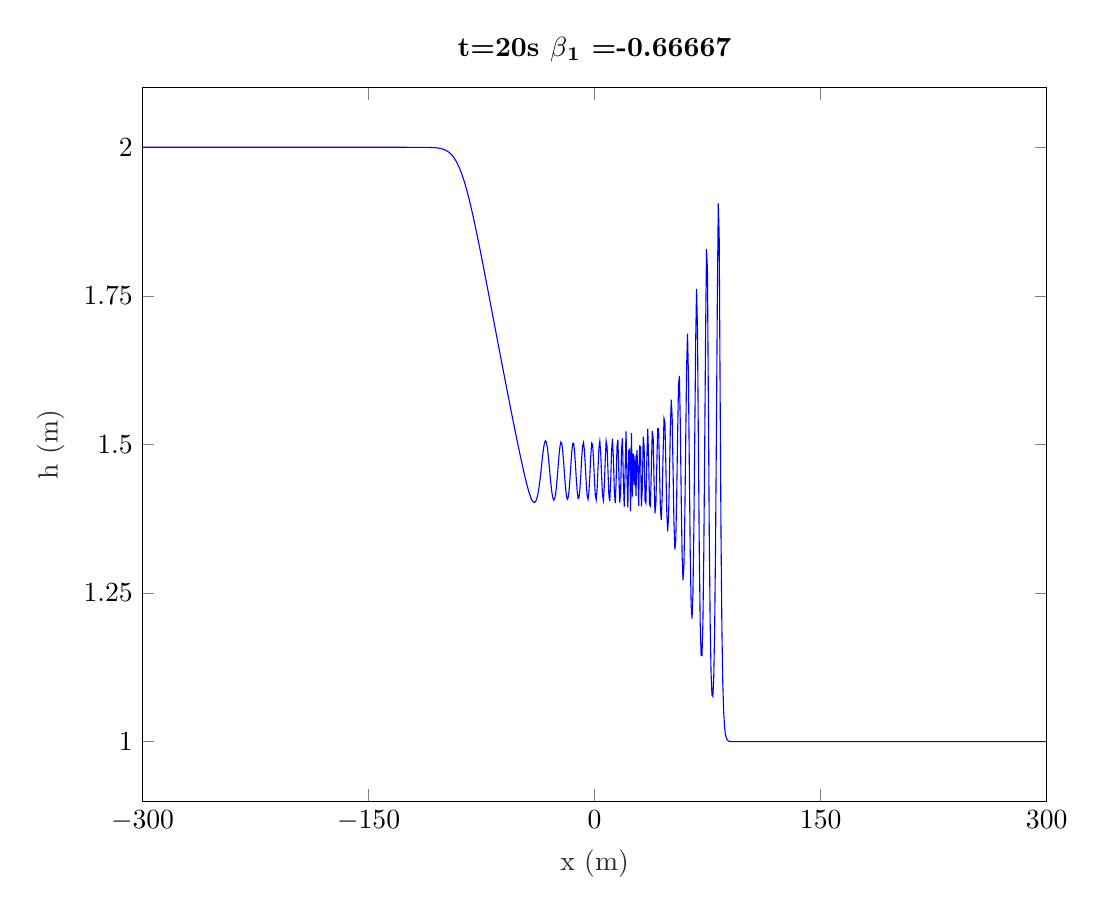
\begin{tikzpicture}

\begin{axis}[%
width=4.521in,
height=3.566in,
at={(0.758in,0.481in)},
scale only axis,
xmin=-300,
xmax=300,
xtick={-300, -150,    0,  150,  300},
xlabel style={font=\color{white!15!black}},
xlabel={x (m)},
ymin=0.9,
ymax=2.1,
ytick={   1, 1.25,  1.5, 1.75,    2},
ylabel style={font=\color{white!15!black}},
ylabel={h (m)},
axis background/.style={fill=white},
title style={font=\bfseries},
title={$\text{t=20s   }\beta{}_\text{1}\text{ =-0.66667}$}
]
\addplot [color=blue, forget plot]
  table[row sep=crcr]{%
-300.18000900045	2\\
-299.57997899895	2\\
-298.97994899745	2\\
-298.37991899595	2\\
-297.77988899445	2\\
-297.17985899295	2\\
-296.57982899145	2\\
-295.979798989949	2\\
-295.379768988449	2\\
-294.779738986949	2\\
-294.179708985449	2\\
-293.579678983949	2\\
-292.979648982449	2\\
-292.379618980949	2\\
-291.779588979449	2\\
-291.179558977949	2\\
-290.579528976449	2\\
-289.979498974949	2\\
-289.379468973449	2\\
-288.779438971949	2\\
-288.179408970449	2\\
-287.579378968948	2\\
-286.979348967448	2\\
-286.379318965948	2\\
-285.779288964448	2\\
-285.179258962948	2\\
-284.579228961448	2\\
-283.979198959948	2\\
-283.379168958448	2\\
-282.779138956948	2\\
-282.179108955448	2\\
-281.579078953948	2\\
-280.979048952448	2\\
-280.379018950948	2\\
-279.778988949447	2\\
-279.178958947947	2\\
-278.578928946447	2\\
-277.978898944947	2\\
-277.378868943447	2\\
-276.778838941947	2\\
-276.178808940447	2\\
-275.578778938947	2\\
-274.978748937447	2\\
-274.378718935947	2\\
-273.778688934447	2\\
-273.178658932947	2\\
-272.578628931447	2\\
-271.978598929946	2\\
-271.378568928446	2\\
-270.778538926946	2\\
-270.178508925446	2\\
-269.578478923946	2\\
-268.978448922446	2\\
-268.378418920946	2\\
-267.778388919446	2\\
-267.178358917946	2\\
-266.578328916446	2\\
-265.978298914946	2\\
-265.378268913446	2\\
-264.778238911946	2\\
-264.178208910446	2\\
-263.578178908945	2\\
-262.978148907445	2\\
-262.378118905945	2\\
-261.778088904445	2\\
-261.178058902945	2\\
-260.578028901445	2\\
-259.977998899945	2\\
-259.377968898445	2\\
-258.777938896945	2\\
-258.177908895445	2\\
-257.577878893945	2\\
-256.977848892445	2\\
-256.377818890945	2\\
-255.777788889444	2\\
-255.177758887944	2\\
-254.577728886444	2\\
-253.977698884944	2\\
-253.377668883444	2\\
-252.777638881944	2\\
-252.177608880444	2\\
-251.577578878944	2\\
-250.977548877444	2\\
-250.377518875944	2\\
-249.777488874444	2\\
-249.177458872944	2\\
-248.577428871444	2\\
-247.977398869943	2\\
-247.377368868443	2\\
-246.777338866943	2\\
-246.177308865443	2\\
-245.577278863943	2\\
-244.977248862443	2\\
-244.377218860943	2\\
-243.777188859443	2\\
-243.177158857943	2\\
-242.577128856443	2\\
-241.977098854943	2\\
-241.377068853443	2\\
-240.777038851943	2\\
-240.177008850443	2\\
-239.576978848942	2\\
-238.976948847442	2\\
-238.376918845942	2\\
-237.776888844442	2\\
-237.176858842942	2\\
-236.576828841442	2\\
-235.976798839942	2\\
-235.376768838442	2\\
-234.776738836942	2\\
-234.176708835442	2\\
-233.576678833942	2\\
-232.976648832442	2\\
-232.376618830942	2\\
-231.776588829441	2\\
-231.176558827941	2\\
-230.576528826441	2\\
-229.976498824941	2\\
-229.376468823441	2\\
-228.776438821941	2\\
-228.176408820441	2\\
-227.576378818941	2\\
-226.976348817441	2\\
-226.376318815941	2\\
-225.776288814441	2\\
-225.176258812941	2\\
-224.576228811441	2\\
-223.976198809941	2\\
-223.37616880844	2\\
-222.77613880694	2\\
-222.17610880544	2\\
-221.57607880394	2\\
-220.97604880244	2\\
-220.37601880094	2\\
-219.77598879944	2\\
-219.17595879794	2\\
-218.57592879644	2\\
-217.97589879494	2\\
-217.37586879344	2\\
-216.77583879194	2\\
-216.17580879044	2\\
-215.575778788939	2\\
-214.975748787439	2\\
-214.375718785939	2\\
-213.775688784439	2\\
-213.175658782939	2\\
-212.575628781439	2\\
-211.975598779939	2\\
-211.375568778439	2\\
-210.775538776939	2\\
-210.175508775439	2\\
-209.575478773939	2\\
-208.975448772439	2\\
-208.375418770939	2\\
-207.775388769438	2\\
-207.175358767938	2\\
-206.575328766438	2\\
-205.975298764938	2\\
-205.375268763438	2\\
-204.775238761938	2\\
-204.175208760438	2\\
-203.575178758938	2\\
-202.975148757438	2\\
-202.375118755938	2\\
-201.775088754438	2\\
-201.175058752938	2\\
-200.575028751438	2\\
-199.974998749937	2\\
-199.374968748437	2\\
-198.774938746937	2\\
-198.174908745437	2\\
-197.574878743937	2\\
-196.974848742437	2\\
-196.374818740937	2\\
-195.774788739437	2\\
-195.174758737937	2\\
-194.574728736437	2\\
-193.974698734937	2\\
-193.374668733437	2\\
-192.774638731937	2\\
-192.174608730437	2\\
-191.574578728936	2\\
-190.974548727436	2\\
-190.374518725936	2\\
-189.774488724436	2\\
-189.174458722936	2\\
-188.574428721436	2\\
-187.974398719936	2\\
-187.374368718436	2\\
-186.774338716936	2\\
-186.174308715436	2\\
-185.574278713936	2\\
-184.974248712436	2\\
-184.374218710936	2\\
-183.774188709435	2\\
-183.174158707935	2\\
-182.574128706435	2\\
-181.974098704935	2\\
-181.374068703435	2\\
-180.774038701935	2\\
-180.174008700435	2\\
-179.573978698935	2\\
-178.973948697435	2\\
-178.373918695935	2\\
-177.773888694435	2\\
-177.173858692935	2\\
-176.573828691435	2\\
-175.973798689934	2\\
-175.373768688434	2\\
-174.773738686934	2\\
-174.173708685434	2\\
-173.573678683934	2\\
-172.973648682434	2\\
-172.373618680934	2\\
-171.773588679434	2\\
-171.173558677934	2\\
-170.573528676434	2\\
-169.973498674934	2\\
-169.373468673434	2\\
-168.773438671934	2\\
-168.173408670434	2\\
-167.573378668933	2\\
-166.973348667433	2\\
-166.373318665933	2\\
-165.773288664433	2\\
-165.173258662933	2\\
-164.573228661433	2\\
-163.973198659933	2\\
-163.373168658433	2\\
-162.773138656933	2\\
-162.173108655433	1.99999999999999\\
-161.573078653933	1.99999999999998\\
-160.973048652433	1.99999999999997\\
-160.373018650933	1.99999999999995\\
-159.772988649432	1.99999999999993\\
-159.172958647932	1.9999999999999\\
-158.572928646432	1.99999999999986\\
-157.972898644932	1.99999999999979\\
-157.372868643432	1.99999999999973\\
-156.772838641932	1.99999999999963\\
-156.172808640432	1.99999999999949\\
-155.572778638932	1.99999999999931\\
-154.972748637432	1.99999999999907\\
-154.372718635932	1.99999999999875\\
-153.772688634432	1.9999999999983\\
-153.172658632932	1.99999999999774\\
-152.572628631432	1.99999999999696\\
-151.972598629931	1.99999999999592\\
-151.372568628431	1.99999999999454\\
-150.772538626931	1.99999999999271\\
-150.172508625431	1.99999999999026\\
-149.572478623931	1.999999999987\\
-148.972448622431	1.99999999998269\\
-148.372418620931	1.99999999997695\\
-147.772388619431	1.99999999996935\\
-147.172358617931	1.99999999995927\\
-146.572328616431	1.99999999994594\\
-145.972298614931	1.9999999999283\\
-145.372268613431	1.99999999990501\\
-144.772238611931	1.99999999987427\\
-144.172208610431	1.99999999983373\\
-143.57217860893	1.99999999978034\\
-142.97214860743	1.9999999997101\\
-142.37211860593	1.99999999961776\\
-141.77208860443	1.9999999994965\\
-141.17205860293	1.99999999933745\\
-140.57202860143	1.99999999912901\\
-139.97199859993	1.99999999885616\\
-139.37196859843	1.99999999849941\\
-138.77193859693	1.9999999980334\\
-138.17190859543	1.99999999742543\\
-137.57187859393	1.99999999663305\\
-136.97184859243	1.99999999560155\\
-136.37181859093	1.9999999942603\\
-135.771788589429	1.99999999251825\\
-135.171758587929	1.99999999025834\\
-134.571728586429	1.99999998733008\\
-133.971698584929	1.99999998354038\\
-133.371668583429	1.99999997864179\\
-132.771638581929	1.99999997231762\\
-132.171608580429	1.99999996416324\\
-131.571578578929	1.99999995366227\\
-130.971548577429	1.99999994015677\\
-130.371518575929	1.99999992280967\\
-129.771488574429	1.99999990055758\\
-129.171458572929	1.99999987205175\\
-128.571428571429	1.99999983558405\\
-127.971398569929	1.99999978899478\\
-127.371368568428	1.99999972955766\\
-126.771338566928	1.99999965383686\\
-126.171308565428	1.99999955750959\\
-125.571278563928	1.99999943514646\\
-124.971248562428	1.99999927994011\\
-124.371218560928	1.99999908337052\\
-123.771188559428	1.99999883479352\\
-123.171158557928	1.99999852093577\\
-122.571128556428	1.99999812527647\\
-121.971098554928	1.99999762729238\\
-121.371068553428	1.99999700153826\\
-120.771038551928	1.99999621652971\\
-120.171008550428	1.99999523338979\\
-119.570978548927	1.99999400421381\\
-118.970948547427	1.99999247009981\\
-118.370918545927	1.99999055878291\\
-117.770888544427	1.99998818180345\\
-117.170858542927	1.99998523112725\\
-116.570828541427	1.99998157512649\\
-115.970798539927	1.99997705381643\\
-115.370768538427	1.9999714732312\\
-114.770738536927	1.99996459880899\\
-114.170708535427	1.99995614764306\\
-113.570678533927	1.99994577944315\\
-112.970648532427	1.99993308603995\\
-112.370618530927	1.99991757925529\\
-111.770588529426	1.99989867695444\\
-111.170558527926	1.99987568709372\\
-110.570528526426	1.99984778957969\\
-109.970498524926	1.99981401576608\\
-109.370468523426	1.9997732254342\\
-108.770438521926	1.99972408113295\\
-108.170408520426	1.99966501979858\\
-107.570378518926	1.99959422163505\\
-106.970348517426	1.99950957631386\\
-106.370318515926	1.99940864665139\\
-105.770288514426	1.99928863004268\\
-105.170258512926	1.99914631807541\\
-104.570228511426	1.99897805491442\\
-103.970198509925	1.99877969523802\\
-103.370168508425	1.99854656271461\\
-102.770138506925	1.99827341023176\\
-102.170108505425	1.99795438331809\\
-101.570078503925	1.99758298842341\\
-100.970048502425	1.99715206793055\\
-100.370018500925	1.99665378394653\\
-99.769988499425	1.9960796130435\\
-99.1699584979249	1.99542035417065\\
-98.5699284964248	1.99466615191575\\
-97.9698984949247	1.99380653713814\\
-97.3698684934247	1.99283048670863\\
-96.7698384919246	1.99172650365968\\
-96.1698084904245	1.99048271846987\\
-95.5697784889244	1.98908701148098\\
-94.9697484874244	1.98752715559372\\
-94.3697184859243	1.98579097743584\\
-93.7696884844242	1.98386653418865\\
-93.1696584829241	1.98174230224938\\
-92.5696284814241	1.97940737296308\\
-91.969598479924	1.97685164984834\\
-91.3695684784239	1.97406604113778\\
-90.7695384769239	1.97104264112034\\
-90.1695084754238	1.9677748937582\\
-89.5694784739237	1.96425773238694\\
-88.9694484724236	1.96048768999962\\
-88.3694184709235	1.95646297563887\\
-87.7693884694235	1.9521835137292\\
-87.1693584679234	1.94765094469441\\
-86.5693284664233	1.9428685868323\\
-85.9692984649232	1.93784136105242\\
-85.3692684634232	1.93257568161749\\
-84.7692384619231	1.92707931736646\\
-84.169208460423	1.92136122895733\\
-83.5691784589229	1.91543138839303\\
-82.9691484574229	1.90930058745611\\
-82.3691184559228	1.90298024167856\\
-81.7690884544227	1.89648219613779\\
-81.1690584529227	1.88981853874991\\
-80.5690284514226	1.88300142589135\\
-79.9689984499225	1.87604292419305\\
-79.3689684484224	1.86895487129582\\
-78.7689384469223	1.86174875729736\\
-78.1689084454223	1.85443562762656\\
-77.5688784439222	1.84702600719115\\
-76.9688484424221	1.83952984489827\\
-76.368818440922	1.83195647705799\\
-75.768788439422	1.82431460775487\\
-75.1687584379219	1.81661230400442\\
-74.5687284364218	1.80885700338468\\
-73.9686984349217	1.80105553182867\\
-73.3686684334217	1.79321412935592\\
-72.7686384319216	1.78533848168773\\
-72.1686084304215	1.77743375590608\\
-71.5685784289215	1.76950463856166\\
-70.9685484274214	1.76155537489173\\
-70.3685184259213	1.75358980806144\\
-69.7684884244212	1.74561141758111\\
-69.1684584229211	1.73762335626956\\
-68.5684284214211	1.7296284853253\\
-67.968398419921	1.72162940723286\\
-67.3683684184209	1.71362849636777\\
-66.7683384169208	1.70562792727594\\
-66.1683084154208	1.69762970068972\\
-65.5682784139207	1.68963566741157\\
-64.9682484124206	1.68164755024533\\
-64.3682184109205	1.67366696419205\\
-63.7681884094205	1.66569543515365\\
-63.1681584079204	1.6577344174063\\
-62.5681284064203	1.64978531012067\\
-61.9680984049203	1.64184947321903\\
-61.3680684034202	1.63392824287447\\
-60.7680384019201	1.62602294697458\\
-60.16800840042	1.6181349208969\\
-59.5679783989199	1.61026552397599\\
-58.9679483974199	1.60241615708622\\
-58.3679183959198	1.59458828182414\\
-57.7678883944197	1.58678344185228\\
-57.1678583929196	1.57900328706898\\
-56.5678283914196	1.57124960140136\\
-55.9677983899195	1.56352433518986\\
-55.3677683884194	1.55582964335306\\
-54.7677383869193	1.54816793080326\\
-54.1677083854193	1.54054190694555\\
-53.5676783839192	1.53295465155636\\
-52.9676483824191	1.5254096949311\\
-52.3676183809191	1.51791111595156\\
-51.767588379419	1.51046366269822\\
-51.1675583779189	1.50307290148041\\
-50.5675283764188	1.49574540175231\\
-49.9674983749187	1.48848896641546\\
-49.3674683734187	1.4813129195896\\
-48.7674383719186	1.47422846718583\\
-48.1674083704185	1.46724914967662\\
-47.5673783689184	1.4603914114487\\
-46.9673483674184	1.45367531712687\\
-46.3673183659183	1.44712545222434\\
-45.7672883644182	1.44077205311108\\
-45.1672583629181	1.4346524188027\\
-44.5672283614181	1.42881266276772\\
-43.967198359918	1.42330986357043\\
-43.3671683584179	1.41821466279725\\
-42.7671383569178	1.41361432715051\\
-42.1671083554178	1.40961622193979\\
-41.5670783539177	1.40635150878181\\
-40.9670483524176	1.40397864138034\\
-40.3670183509175	1.40268583539934\\
-39.7669883494175	1.40269101897216\\
-39.1669583479174	1.40423724592492\\
-38.5669283464173	1.40757914905622\\
-37.9668983449172	1.41295714220522\\
-37.3668683434172	1.42055258257982\\
-36.7668383419171	1.43042037477165\\
-36.166808340417	1.44239896343769\\
-35.5667783389169	1.45600911930596\\
-34.9667483374168	1.47037050796245\\
-34.3667183359168	1.48418444599004\\
-33.7666883344167	1.49583875159386\\
-33.1666583329167	1.50366520532823\\
-32.5666283314166	1.50630860348138\\
-31.9665983299165	1.50311622155472\\
-31.3665683284164	1.49431420867694\\
-30.7665383269164	1.48101446205025\\
-30.1665083254163	1.46494002730117\\
-29.5664783239162	1.44807217347912\\
-28.9664483224161	1.43232600086057\\
-28.3664183209161	1.41934369127398\\
-27.766388319416	1.41041329343331\\
-27.1663583179159	1.40646856173511\\
-26.5663283164158	1.40809902188238\\
-25.9662983149157	1.41550340622954\\
-25.3662683134157	1.4283477969957\\
-24.7662383119156	1.44553553249537\\
-24.1662083104155	1.46498481878096\\
-23.5661783089154	1.48361139259959\\
-22.9661483074154	1.4977546440023\\
-22.3661183059153	1.50412164570116\\
-21.7660883044152	1.50092688640607\\
-21.1660583029151	1.48864421520876\\
-20.5660283014151	1.46988527161972\\
-19.965998299915	1.44857279553226\\
-19.3659682984149	1.42888464557757\\
-18.7659382969148	1.41443544648454\\
-18.1659082954148	1.40784040567646\\
-17.5658782939147	1.41052676405425\\
-16.9658482924146	1.42254516431412\\
-16.3658182909145	1.44222962312402\\
-15.7657882894144	1.46583043627693\\
-15.1657582879144	1.48764652390231\\
-14.5657282864143	1.50131113116669\\
-13.9656982849143	1.50220822380473\\
-13.3656682834142	1.4896976870687\\
-12.7656382819141	1.46752389679965\\
-12.165608280414	1.44222839823021\\
-11.565578278914	1.42084408227803\\
-10.9655482774139	1.409081613653\\
-10.3655182759138	1.41031401024644\\
-9.76548827441371	1.42495311093804\\
-9.16545827291367	1.44977798690119\\
-8.56542827141357	1.47753582920734\\
-7.96539826991352	1.49821624956484\\
-7.36536826841342	1.50311172557956\\
-6.76533826691332	1.48971677419612\\
-6.16530826541327	1.46336524016465\\
-5.56527826391317	1.43430668678964\\
-4.96524826241313	1.41325380386242\\
-4.36521826091303	1.40796312342459\\
-3.76518825941298	1.42123118391724\\
-3.16515825791288	1.44937978591579\\
-2.56512825641283	1.48150839613594\\
-1.96509825491273	1.50224044771073\\
-1.36506825341269	1.50013285420386\\
-0.765038251912586	1.47591736918839\\
-0.165008250412541	1.44194668911743\\
0.435021751087561	1.41463283750327\\
1.03505175258761	1.40704461502559\\
1.63508175408771	1.42410474884491\\
2.23511175558775	1.45929400989516\\
2.83514175708785	1.49388073543015\\
3.43517175858796	1.50542371854571\\
4.035201760088	1.48561808662463\\
4.6352317615881	1.44726407618833\\
5.23526176308815	1.41406484187047\\
5.83529176458825	1.40624348403404\\
6.43532176608829	1.43080528577106\\
7.03535176758839	1.47458887535348\\
7.63538176908844	1.50565479925192\\
8.23541177058854	1.49733019033701\\
8.83544177208859	1.45636766959962\\
9.43547177358869	1.4149571531315\\
10.0355017750887	1.40469954066338\\
10.6355317765888	1.43707044219615\\
11.2355617780889	1.48889864425528\\
11.835591779589	1.50959056416075\\
12.435621781089	1.47667043388948\\
13.0356517825891	1.42363317212941\\
13.6356817840892	1.40123901996639\\
14.2357117855893	1.43547451945075\\
14.8357417870894	1.49667123332639\\
15.4357717885894	1.5081434442844\\
16.0358017900895	1.45402465995111\\
16.6358317915896	1.40241235350832\\
17.2358617930897	1.41792679399426\\
17.8358917945897	1.49171232536117\\
18.4359217960898	1.51048345382093\\
19.0359517975899	1.44145844660079\\
19.63598179909	1.39540120530638\\
20.23601180059	1.45436986512574\\
20.8360418020901	1.52189354592373\\
21.4360718035902	1.44849404903228\\
22.0361018050903	1.39369101282264\\
22.6361318065904	1.48949816887977\\
23.2361618080904	1.49172017491654\\
23.8361918095905	1.38849299603205\\
24.4362218110905	1.51910585619918\\
25.0362518125906	1.41233348631789\\
25.6362818140907	1.48456625968838\\
26.2363118155908	1.43206631569216\\
26.8363418170908	1.48159790135754\\
27.4363718185909	1.41367655552578\\
28.036401820091	1.49084798639232\\
28.6364318215911	1.46272502156727\\
29.2364618230911	1.39657423562311\\
29.8364918245912	1.49741528836618\\
30.4365218260913	1.49643664670824\\
31.0365518275914	1.39602018019772\\
31.6365818290914	1.42555645280434\\
32.2366118305915	1.51327417018109\\
32.8366418320916	1.49593042907795\\
33.4366718335917	1.40552181036088\\
34.0367018350918	1.40116587625908\\
34.6367318365918	1.47488667035863\\
35.2367618380919	1.52626428062309\\
35.836791839592	1.4748648194858\\
36.4368218410921	1.39915842957248\\
37.0368518425921	1.39620788939136\\
37.6368818440922	1.45969477440663\\
38.2369118455923	1.52256686636041\\
38.8369418470924	1.51133152705251\\
39.4369718485924	1.43622928517058\\
40.0370018500925	1.38419613317802\\
40.6370318515926	1.39974366995618\\
41.2370618530927	1.46490994775262\\
41.8370918545928	1.52650581627466\\
42.4371218560928	1.52636072241198\\
43.0371518575929	1.45990187453873\\
43.6371818590929	1.39108991604883\\
44.237211860593	1.37319247965748\\
44.8372418620931	1.41402001171942\\
45.4372718635932	1.48688404065335\\
46.0373018650932	1.54381374416732\\
46.6373318665933	1.53735956596143\\
47.2373618680934	1.46729139796823\\
47.8373918695935	1.38939616268856\\
48.4374218710935	1.35389728476088\\
49.0374518725936	1.37656868448538\\
49.6374818740937	1.44600487053177\\
50.2375118755938	1.52862943122743\\
50.8375418770938	1.5753860185931\\
51.4375718785939	1.54656757456915\\
52.037601880094	1.45686611573598\\
52.6376318815941	1.36724390646024\\
53.2376618830942	1.32299427103548\\
53.8376918845942	1.338990014912\\
54.4377218860943	1.41012535567249\\
55.0377518875944	1.51200519005424\\
55.6377818890945	1.59939906920205\\
56.2378118905945	1.61554291773756\\
56.8378418920946	1.53571146470177\\
57.4378718935947	1.41166422950373\\
58.0379018950948	1.31287835248093\\
58.6379318965948	1.27150888377138\\
59.2379618980949	1.29483434494277\\
59.837991899595	1.3795790059377\\
60.4380219010951	1.50634824391439\\
61.0380519025952	1.63097461706905\\
61.6380819040952	1.68639223681277\\
62.2381119055953	1.61497949227506\\
62.8381419070953	1.45929207656902\\
63.4381719085955	1.3151892575987\\
64.0382019100955	1.2289392500393\\
64.6382319115956	1.20708565210013\\
65.2382619130956	1.24966059715264\\
65.8382919145957	1.35646624563221\\
66.4383219160958	1.51258038385137\\
67.0383519175959	1.67329654721256\\
67.6383819190959	1.76191725157175\\
68.238411920596	1.69378828492362\\
68.8384419220961	1.50301103956579\\
69.4384719235962	1.31940238171815\\
70.0385019250962	1.20027014853956\\
70.6385319265963	1.14490882191134\\
71.2385619280964	1.14462404837117\\
71.8385919295965	1.19999619719326\\
72.4386219310966	1.31852354646336\\
73.0386519325966	1.49508024432064\\
73.6386819340967	1.69015403460561\\
74.2387119355968	1.82886352028687\\
74.8387419370969	1.79551666873918\\
75.4387719385969	1.58425262070195\\
76.038801940097	1.35826203987732\\
76.6388319415971	1.20354860408085\\
77.2388619430972	1.11697518615664\\
77.8388919445972	1.07860443346991\\
78.4389219460973	1.07609052774869\\
79.0389519475974	1.10909740735777\\
79.6389819490975	1.18899752307361\\
80.2390119505975	1.33181321013106\\
80.8390419520976	1.53448102430648\\
81.4390719535977	1.7531192600295\\
82.0391019550977	1.90555565718384\\
82.6391319565979	1.85260307669355\\
83.2391619580979	1.60127707003583\\
83.839191959598	1.35315180254726\\
84.439221961098	1.19017223159649\\
85.0392519625981	1.09789132655322\\
85.6392819640982	1.0491410034806\\
86.2393119655983	1.02433693899933\\
86.8393419670983	1.01196910088089\\
87.4393719685984	1.00586616461016\\
88.0394019700985	1.00287028113635\\
88.6394319715986	1.00140333993565\\
89.2394619730986	1.00068590394561\\
89.8394919745987	1.00033521348404\\
90.4395219760988	1.00016382681885\\
91.0395519775989	1.00008007147122\\
91.639581979099	1.00003913923415\\
92.239611980599	1.00001913354065\\
92.8396419820991	1.00000935472344\\
93.4396719835992	1.00000457427153\\
94.0397019850993	1.00000223702323\\
94.6397319865993	1.00000109415423\\
95.2397619880994	1.0000005352392\\
95.8397919895995	1.00000026186678\\
96.4398219910996	1.00000012813799\\
97.0398519925996	1.00000006271079\\
97.6398819940997	1.00000003069555\\
98.2399119955998	1.00000001502725\\
98.8399419970999	1.00000000735794\\
99.4399719985999	1.00000000360336\\
100.0400020001	1.00000000176497\\
100.6400320016	1.00000000086465\\
101.2400620031	1.00000000042367\\
101.8400920046	1.00000000020764\\
102.4401220061	1.00000000010177\\
103.0401520076	1.00000000004989\\
103.6401820091	1.00000000002447\\
104.240212010601	1.00000000001199\\
104.840242012101	1.00000000000588\\
105.440272013601	1.00000000000289\\
106.040302015101	1.00000000000141\\
106.640332016601	1.00000000000069\\
107.240362018101	1.00000000000033\\
107.840392019601	1.00000000000016\\
108.440422021101	1.00000000000008\\
109.040452022601	1.00000000000003\\
109.640482024101	1.00000000000001\\
110.240512025601	1\\
110.840542027101	1\\
111.440572028601	1\\
112.040602030102	1\\
112.640632031602	1\\
113.240662033102	1\\
113.840692034602	1\\
114.440722036102	1\\
115.040752037602	1\\
115.640782039102	1\\
116.240812040602	1\\
116.840842042102	1\\
117.440872043602	1\\
118.040902045102	1\\
118.640932046602	1\\
119.240962048102	1\\
119.840992049603	1\\
120.441022051103	1\\
121.041052052603	1\\
121.641082054103	1\\
122.241112055603	1\\
122.841142057103	1\\
123.441172058603	1\\
124.041202060103	1\\
124.641232061603	1\\
125.241262063103	1\\
125.841292064603	1\\
126.441322066103	1\\
127.041352067603	1\\
127.641382069103	1\\
128.241412070604	1\\
128.841442072104	1\\
129.441472073604	1\\
130.041502075104	1\\
130.641532076604	1\\
131.241562078104	1\\
131.841592079604	1\\
132.441622081104	1\\
133.041652082604	1\\
133.641682084104	1\\
134.241712085604	1\\
134.841742087104	1\\
135.441772088604	1\\
136.041802090105	1\\
136.641832091605	1\\
137.241862093105	1\\
137.841892094605	1\\
138.441922096105	1\\
139.041952097605	1\\
139.641982099105	1\\
140.242012100605	1\\
140.842042102105	1\\
141.442072103605	1\\
142.042102105105	1\\
142.642132106605	1\\
143.242162108105	1\\
143.842192109605	1\\
144.442222111106	1\\
145.042252112606	1\\
145.642282114106	1\\
146.242312115606	1\\
146.842342117106	1\\
147.442372118606	1\\
148.042402120106	1\\
148.642432121606	1\\
149.242462123106	1\\
149.842492124606	1\\
150.442522126106	1\\
151.042552127606	1\\
151.642582129106	1\\
152.242612130607	1\\
152.842642132107	1\\
153.442672133607	1\\
154.042702135107	1\\
154.642732136607	1\\
155.242762138107	1\\
155.842792139607	1\\
156.442822141107	1\\
157.042852142607	1\\
157.642882144107	1\\
158.242912145607	1\\
158.842942147107	1\\
159.442972148607	1\\
160.043002150107	1\\
160.643032151608	1\\
161.243062153108	1\\
161.843092154608	1\\
162.443122156108	1\\
163.043152157608	1\\
163.643182159108	1\\
164.243212160608	1\\
164.843242162108	1\\
165.443272163608	1\\
166.043302165108	1\\
166.643332166608	1\\
167.243362168108	1\\
167.843392169608	1\\
168.443422171109	1\\
169.043452172609	1\\
169.643482174109	1\\
170.243512175609	1\\
170.843542177109	1\\
171.443572178609	1\\
172.043602180109	1\\
172.643632181609	1\\
173.243662183109	1\\
173.843692184609	1\\
174.443722186109	1\\
175.043752187609	1\\
175.643782189109	1\\
176.24381219061	1\\
176.84384219211	1\\
177.44387219361	1\\
178.04390219511	1\\
178.64393219661	1\\
179.24396219811	1\\
179.84399219961	1\\
180.44402220111	1\\
181.04405220261	1\\
181.64408220411	1\\
182.24411220561	1\\
182.84414220711	1\\
183.44417220861	1\\
184.04420221011	1\\
184.644232211611	1\\
185.244262213111	1\\
185.844292214611	1\\
186.444322216111	1\\
187.044352217611	1\\
187.644382219111	1\\
188.244412220611	1\\
188.844442222111	1\\
189.444472223611	1\\
190.044502225111	1\\
190.644532226611	1\\
191.244562228111	1\\
191.844592229611	1\\
192.444622231112	1\\
193.044652232612	1\\
193.644682234112	1\\
194.244712235612	1\\
194.844742237112	1\\
195.444772238612	1\\
196.044802240112	1\\
196.644832241612	1\\
197.244862243112	1\\
197.844892244612	1\\
198.444922246112	1\\
199.044952247612	1\\
199.644982249112	1\\
200.245012250613	1\\
200.845042252113	1\\
201.445072253613	1\\
202.045102255113	1\\
202.645132256613	1\\
203.245162258113	1\\
203.845192259613	1\\
204.445222261113	1\\
205.045252262613	1\\
205.645282264113	1\\
206.245312265613	1\\
206.845342267113	1\\
207.445372268613	1\\
208.045402270114	1\\
208.645432271614	1\\
209.245462273114	1\\
209.845492274614	1\\
210.445522276114	1\\
211.045552277614	1\\
211.645582279114	1\\
212.245612280614	1\\
212.845642282114	1\\
213.445672283614	1\\
214.045702285114	1\\
214.645732286614	1\\
215.245762288114	1\\
215.845792289614	1\\
216.445822291115	1\\
217.045852292615	1\\
217.645882294115	1\\
218.245912295615	1\\
218.845942297115	1\\
219.445972298615	1\\
220.046002300115	1\\
220.646032301615	1\\
221.246062303115	1\\
221.846092304615	1\\
222.446122306115	1\\
223.046152307615	1\\
223.646182309115	1\\
224.246212310616	1\\
224.846242312116	1\\
225.446272313616	1\\
226.046302315116	1\\
226.646332316616	1\\
227.246362318116	1\\
227.846392319616	1\\
228.446422321116	1\\
229.046452322616	1\\
229.646482324116	1\\
230.246512325616	1\\
230.846542327116	1\\
231.446572328616	1\\
232.046602330116	1\\
232.646632331617	1\\
233.246662333117	1\\
233.846692334617	1\\
234.446722336117	1\\
235.046752337617	1\\
235.646782339117	1\\
236.246812340617	1\\
236.846842342117	1\\
237.446872343617	1\\
238.046902345117	1\\
238.646932346617	1\\
239.246962348117	1\\
239.846992349617	1\\
240.447022351118	1\\
241.047052352618	1\\
241.647082354118	1\\
242.247112355618	1\\
242.847142357118	1\\
243.447172358618	1\\
244.047202360118	1\\
244.647232361618	1\\
245.247262363118	1\\
245.847292364618	1\\
246.447322366118	1\\
247.047352367618	1\\
247.647382369118	1\\
248.247412370619	1\\
248.847442372119	1\\
249.447472373619	1\\
250.047502375119	1\\
250.647532376619	1\\
251.247562378119	1\\
251.847592379619	1\\
252.447622381119	1\\
253.047652382619	1\\
253.647682384119	1\\
254.247712385619	1\\
254.847742387119	1\\
255.447772388619	1\\
256.04780239012	1\\
256.64783239162	1\\
257.24786239312	1\\
257.84789239462	1\\
258.44792239612	1\\
259.04795239762	1\\
259.64798239912	1\\
260.24801240062	1\\
260.84804240212	1\\
261.44807240362	1\\
262.04810240512	1\\
262.64813240662	1\\
263.24816240812	1\\
263.84819240962	1\\
264.448222411121	1\\
265.048252412621	1\\
265.648282414121	1\\
266.248312415621	1\\
266.848342417121	1\\
267.448372418621	1\\
268.048402420121	1\\
268.648432421621	1\\
269.248462423121	1\\
269.848492424621	1\\
270.448522426121	1\\
271.048552427621	1\\
271.648582429121	1\\
272.248612430622	1\\
272.848642432122	1\\
273.448672433622	1\\
274.048702435122	1\\
274.648732436622	1\\
275.248762438122	1\\
275.848792439622	1\\
276.448822441122	1\\
277.048852442622	1\\
277.648882444122	1\\
278.248912445622	1\\
278.848942447122	1\\
279.448972448622	1\\
280.049002450123	1\\
280.649032451623	1\\
281.249062453123	1\\
281.849092454623	1\\
282.449122456123	1\\
283.049152457623	1\\
283.649182459123	1\\
284.249212460623	1\\
284.849242462123	1\\
285.449272463623	1\\
286.049302465123	1\\
286.649332466623	1\\
287.249362468123	1\\
287.849392469623	1\\
288.449422471124	1\\
289.049452472624	1\\
289.649482474124	1\\
290.249512475624	1\\
290.849542477124	1\\
291.449572478624	1\\
292.049602480124	1\\
292.649632481624	1\\
293.249662483124	1\\
293.849692484624	1\\
294.449722486124	1\\
295.049752487624	1\\
295.649782489125	1\\
296.249812490625	1\\
296.849842492125	1\\
297.449872493625	1\\
298.049902495125	1\\
298.649932496625	1\\
299.249962498125	1\\
299.849992499625	1\\
};
\end{axis}
\end{tikzpicture}%
		\caption{$t=20s$}
	\end{subfigure}
	\begin{subfigure}{0.49\textwidth}
		\centering
		% This file was created by matlab2tikz.
%
%The latest updates can be retrieved from
%  http://www.mathworks.com/matlabcentral/fileexchange/22022-matlab2tikz-matlab2tikz
%where you can also make suggestions and rate matlab2tikz.
%
\begin{tikzpicture}

\begin{axis}[%
width=4.521in,
height=3.566in,
at={(0.758in,0.481in)},
scale only axis,
xmin=-300,
xmax=300,
xtick={-300, -150,    0,  150,  300},
xlabel style={font=\color{white!15!black}},
xlabel={x (m)},
ymin=0.9,
ymax=2.1,
ytick={   1, 1.25,  1.5, 1.75,    2},
ylabel style={font=\color{white!15!black}},
ylabel={h (m)},
axis background/.style={fill=white},
title style={font=\bfseries},
title={$\text{t=30s   }\beta{}_\text{1}\text{ =-0.66667}$}
]
\addplot [color=blue, forget plot]
  table[row sep=crcr]{%
-300.18000900045	2\\
-299.57997899895	2\\
-298.97994899745	2\\
-298.37991899595	2\\
-297.77988899445	2\\
-297.17985899295	2\\
-296.57982899145	2\\
-295.979798989949	2\\
-295.379768988449	2\\
-294.779738986949	2\\
-294.179708985449	2\\
-293.579678983949	2\\
-292.979648982449	2\\
-292.379618980949	2\\
-291.779588979449	2\\
-291.179558977949	2\\
-290.579528976449	2\\
-289.979498974949	2\\
-289.379468973449	2\\
-288.779438971949	2\\
-288.179408970449	2\\
-287.579378968948	2\\
-286.979348967448	2\\
-286.379318965948	2\\
-285.779288964448	2\\
-285.179258962948	2\\
-284.579228961448	2\\
-283.979198959948	2\\
-283.379168958448	2\\
-282.779138956948	2\\
-282.179108955448	2\\
-281.579078953948	2\\
-280.979048952448	2\\
-280.379018950948	2\\
-279.778988949447	2\\
-279.178958947947	2\\
-278.578928946447	2\\
-277.978898944947	2\\
-277.378868943447	2\\
-276.778838941947	2\\
-276.178808940447	2\\
-275.578778938947	2\\
-274.978748937447	2\\
-274.378718935947	2\\
-273.778688934447	2\\
-273.178658932947	2\\
-272.578628931447	2\\
-271.978598929946	2\\
-271.378568928446	2\\
-270.778538926946	2\\
-270.178508925446	2\\
-269.578478923946	2\\
-268.978448922446	2\\
-268.378418920946	2\\
-267.778388919446	2\\
-267.178358917946	2\\
-266.578328916446	2\\
-265.978298914946	2\\
-265.378268913446	2\\
-264.778238911946	2\\
-264.178208910446	2\\
-263.578178908945	2\\
-262.978148907445	2\\
-262.378118905945	2\\
-261.778088904445	2\\
-261.178058902945	2\\
-260.578028901445	2\\
-259.977998899945	2\\
-259.377968898445	2\\
-258.777938896945	2\\
-258.177908895445	2\\
-257.577878893945	2\\
-256.977848892445	2\\
-256.377818890945	2\\
-255.777788889444	2\\
-255.177758887944	2\\
-254.577728886444	2\\
-253.977698884944	2\\
-253.377668883444	2\\
-252.777638881944	2\\
-252.177608880444	2\\
-251.577578878944	2\\
-250.977548877444	2\\
-250.377518875944	2\\
-249.777488874444	2\\
-249.177458872944	2\\
-248.577428871444	2\\
-247.977398869943	2\\
-247.377368868443	2\\
-246.777338866943	2\\
-246.177308865443	2\\
-245.577278863943	2\\
-244.977248862443	2\\
-244.377218860943	2\\
-243.777188859443	2\\
-243.177158857943	2\\
-242.577128856443	2\\
-241.977098854943	2\\
-241.377068853443	2\\
-240.777038851943	2\\
-240.177008850443	2\\
-239.576978848942	2\\
-238.976948847442	2\\
-238.376918845942	2\\
-237.776888844442	2\\
-237.176858842942	2\\
-236.576828841442	2\\
-235.976798839942	2\\
-235.376768838442	2\\
-234.776738836942	2\\
-234.176708835442	2\\
-233.576678833942	2\\
-232.976648832442	2\\
-232.376618830942	2\\
-231.776588829441	2\\
-231.176558827941	2\\
-230.576528826441	2\\
-229.976498824941	2\\
-229.376468823441	2\\
-228.776438821941	2\\
-228.176408820441	2\\
-227.576378818941	2\\
-226.976348817441	2\\
-226.376318815941	2\\
-225.776288814441	2\\
-225.176258812941	2\\
-224.576228811441	2\\
-223.976198809941	2\\
-223.37616880844	2\\
-222.77613880694	2\\
-222.17610880544	2\\
-221.57607880394	2\\
-220.97604880244	2\\
-220.37601880094	2\\
-219.77598879944	2\\
-219.17595879794	2\\
-218.57592879644	2\\
-217.97589879494	2\\
-217.37586879344	2\\
-216.77583879194	2\\
-216.17580879044	2\\
-215.575778788939	2\\
-214.975748787439	2\\
-214.375718785939	2\\
-213.775688784439	2\\
-213.175658782939	2\\
-212.575628781439	2\\
-211.975598779939	2\\
-211.375568778439	2\\
-210.775538776939	2\\
-210.175508775439	2\\
-209.575478773939	2\\
-208.975448772439	2\\
-208.375418770939	2\\
-207.775388769438	2\\
-207.175358767938	2\\
-206.575328766438	1.99999999999999\\
-205.975298764938	1.99999999999999\\
-205.375268763438	1.99999999999997\\
-204.775238761938	1.99999999999996\\
-204.175208760438	1.99999999999994\\
-203.575178758938	1.99999999999991\\
-202.975148757438	1.99999999999988\\
-202.375118755938	1.99999999999984\\
-201.775088754438	1.99999999999977\\
-201.175058752938	1.99999999999968\\
-200.575028751438	1.99999999999957\\
-199.974998749937	1.99999999999941\\
-199.374968748437	1.99999999999921\\
-198.774938746937	1.99999999999893\\
-198.174908745437	1.99999999999856\\
-197.574878743937	1.99999999999806\\
-196.974848742437	1.9999999999974\\
-196.374818740937	1.99999999999651\\
-195.774788739437	1.99999999999533\\
-195.174758737937	1.99999999999375\\
-194.574728736437	1.99999999999164\\
-193.974698734937	1.99999999998885\\
-193.374668733437	1.99999999998513\\
-192.774638731937	1.99999999998019\\
-192.174608730437	1.99999999997363\\
-191.574578728936	1.99999999996493\\
-190.974548727436	1.99999999995342\\
-190.374518725936	1.99999999993817\\
-189.774488724436	1.99999999991802\\
-189.174458722936	1.9999999998914\\
-188.574428721436	1.99999999985626\\
-187.974398719936	1.99999999980995\\
-187.374368718436	1.99999999974896\\
-186.774338716936	1.99999999966871\\
-186.174308715436	1.99999999956324\\
-185.574278713936	1.99999999942477\\
-184.974248712436	1.99999999924315\\
-184.374218710936	1.9999999990052\\
-183.774188709435	1.99999999869378\\
-183.174158707935	1.99999999828664\\
-182.574128706435	1.99999999775494\\
-181.974098704935	1.99999999706136\\
-181.374068703435	1.9999999961576\\
-180.774038701935	1.99999999498133\\
-180.174008700435	1.99999999345213\\
-179.573978698935	1.99999999146644\\
-178.973948697435	1.99999998889099\\
-178.373918695935	1.99999998555465\\
-177.773888694435	1.9999999812378\\
-177.173858692935	1.99999997565916\\
-176.573828691435	1.99999996845882\\
-175.973798689934	1.99999995917708\\
-175.373768688434	1.99999994722745\\
-174.773738686934	1.99999993186301\\
-174.173708685434	1.99999991213373\\
-173.573678683934	1.99999988683322\\
-172.973648682434	1.99999985443192\\
-172.373618680934	1.99999981299352\\
-171.773588679434	1.99999976007081\\
-171.173558677934	1.9999996925759\\
-170.573528676434	1.99999960661893\\
-169.973498674934	1.99999949730826\\
-169.373468673434	1.99999935850282\\
-168.773438671934	1.99999918250689\\
-168.173408670434	1.99999895969359\\
-167.573378668933	1.99999867804247\\
-166.973348667433	1.99999832257244\\
-166.373318665933	1.9999978746482\\
-165.773288664433	1.99999731113416\\
-165.173258662933	1.999996603365\\
-164.573228661433	1.99999571589648\\
-163.973198659933	1.9999946049939\\
-163.373168658433	1.99999321680865\\
-162.773138656933	1.9999914851848\\
-162.173108655433	1.99998932902955\\
-161.573078653933	1.99998664917087\\
-160.973048652433	1.99998332461581\\
-160.373018650933	1.9999792081112\\
-159.772988649432	1.99997412089731\\
-159.172958647932	1.999967846533\\
-158.572928646432	1.99996012365993\\
-157.972898644932	1.99995063756261\\
-157.372868643432	1.99993901037341\\
-156.772838641932	1.99992478976575\\
-156.172808640432	1.99990743597813\\
-155.572778638932	1.99988630701731\\
-154.972748637432	1.99986064190206\\
-154.372718635932	1.99982954183426\\
-153.772688634432	1.99979194922173\\
-153.172658632932	1.99974662453237\\
-152.572628631432	1.99969212103407\\
-151.972598629931	1.99962675757251\\
-151.372568628431	1.99954858966275\\
-150.772538626931	1.99945537932153\\
-150.172508625431	1.9993445642457\\
-149.572478623931	1.99921322714678\\
-148.972448622431	1.99905806627642\\
-148.372418620931	1.9988753684135\\
-147.772388619431	1.99866098581681\\
-147.172358617931	1.99841031885837\\
-146.572328616431	1.99811830621671\\
-145.972298614931	1.99777942459805\\
-145.372268613431	1.99738769993436\\
-144.772238611931	1.99693673185135\\
-144.172208610431	1.9964197328798\\
-143.57217860893	1.99582958338674\\
-142.97214860743	1.99515890253071\\
-142.37211860593	1.99440013471955\\
-141.77208860443	1.99354565011772\\
-141.17205860293	1.9925878567815\\
-140.57202860143	1.99151932108192\\
-139.97199859993	1.9903328923025\\
-139.37196859843	1.98902182676173\\
-138.77193859693	1.98757990658161\\
-138.17190859543	1.98600154834318\\
-137.57187859393	1.98428189733992\\
-136.97184859243	1.98241690392004\\
-136.37181859093	1.98040337942234\\
-135.771788589429	1.97823903035954\\
-135.171758587929	1.97592247067429\\
-134.571728586429	1.97345321298621\\
-133.971698584929	1.97083164067617\\
-133.371668583429	1.96805896336068\\
-132.771638581929	1.96513715876831\\
-132.171608580429	1.96206890424359\\
-131.571578578929	1.95885750109834\\
-130.971548577429	1.95550679484522\\
-130.371518575929	1.95202109403383\\
-129.771488574429	1.94840509001216\\
-129.171458572929	1.94466377950224\\
-128.571428571429	1.94080239144263\\
-127.971398569929	1.93682631913981\\
-127.371368568428	1.93274105840406\\
-126.771338566928	1.92855215203128\\
-126.171308565428	1.92426514073596\\
-125.571278563928	1.91988552043873\\
-124.971248562428	1.91541870566211\\
-124.371218560928	1.91086999868152\\
-123.771188559428	1.90624456401077\\
-123.171158557928	1.9015474077625\\
-122.571128556428	1.89678336140971\\
-121.971098554928	1.8919570694769\\
-121.371068553428	1.88707298070535\\
-120.771038551928	1.88213534226066\\
-120.171008550428	1.87714819658004\\
-119.570978548927	1.87211538048894\\
-118.970948547427	1.86704052624925\\
-118.370918545927	1.8619270642342\\
-117.770888544427	1.85677822695629\\
-117.170858542927	1.85159705420407\\
-116.570828541427	1.84638639907117\\
-115.970798539927	1.84114893468626\\
-115.370768538427	1.83588716147581\\
-114.770738536927	1.83060341481219\\
-114.170708535427	1.82529987291909\\
-113.570678533927	1.81997856492315\\
-112.970648532427	1.81464137895609\\
-112.370618530927	1.80929007022597\\
-111.770588529426	1.80392626898843\\
-111.170558527926	1.7985514883603\\
-110.570528526426	1.7931671319282\\
-109.970498524926	1.7877745011138\\
-109.370468523426	1.78237480226569\\
-108.770438521926	1.77696915345519\\
-108.170408520426	1.77155859095986\\
-107.570378518926	1.76614407542435\\
-106.970348517426	1.76072649769306\\
-106.370318515926	1.75530668431376\\
-105.770288514426	1.74988540271491\\
-105.170258512926	1.74446336606268\\
-104.570228511426	1.73904123780634\\
-103.970198509925	1.73361963592303\\
-103.370168508425	1.7281991368745\\
-102.770138506925	1.72278027929001\\
-102.170108505425	1.71736356739058\\
-101.570078503925	1.71194947417027\\
-100.970048502425	1.70653844435137\\
-100.370018500925	1.70113089712962\\
-99.769988499425	1.6957272287268\\
-99.1699584979249	1.69032781476711\\
-98.5699284964248	1.68493301249409\\
-97.9698984949247	1.67954316284457\\
-97.3698684934247	1.67415859239567\\
-96.7698384919246	1.66877961520086\\
-96.1698084904245	1.66340653453078\\
-95.5697784889244	1.65803964453421\\
-94.9697484874244	1.65267923183445\\
-94.3697184859243	1.6473255770767\\
-93.7696884844242	1.64197895644136\\
-93.1696584829241	1.63663964313943\\
-92.5696284814241	1.63130790890548\\
-91.969598479924	1.62598402550517\\
-91.3695684784239	1.62066826627469\\
-90.7695384769239	1.61536090771065\\
-90.1695084754238	1.61006223113061\\
-89.5694784739237	1.60477252442601\\
-88.9694484724236	1.59949208393167\\
-88.3694184709235	1.59422121643896\\
-87.7693884694235	1.5889602413827\\
-87.1693584679234	1.58370949323658\\
-86.5693284664233	1.57846932415647\\
-85.9692984649232	1.57324010691712\\
-85.3692684634232	1.56802223819527\\
-84.7692384619231	1.56281614226071\\
-84.169208460423	1.55762227514781\\
-83.5691784589229	1.5524411293927\\
-82.9691484574229	1.5472732394372\\
-82.3691184559228	1.54211918781963\\
-81.7690884544227	1.53697961229588\\
-81.1690584529227	1.53185521406292\\
-80.5690284514226	1.52674676729205\\
-79.9689984499225	1.52165513022261\\
-79.3689684484224	1.51658125812099\\
-78.7689384469223	1.51152621847727\\
-78.1689084454223	1.50649120889633\\
-77.5688784439222	1.50147757824712\\
-76.9688484424221	1.49648685176989\\
-76.368818440922	1.49152076101471\\
-75.768788439422	1.48658127970957\\
-75.1687584379219	1.48167066694766\\
-74.5687284364218	1.47679151946769\\
-73.9686984349217	1.47194683530877\\
-73.3686684334217	1.46714009180397\\
-72.7686384319216	1.46237534180124\\
-72.1686084304215	1.45765733327186\\
-71.5685784289215	1.45299165923877\\
-70.9685484274214	1.44838494746625\\
-70.3685184259213	1.44384510296538\\
-69.7684884244212	1.43938162167159\\
-69.1684584229211	1.43500600159488\\
-68.5684284214211	1.43073228992403\\
-67.968398419921	1.42657782373718\\
-67.3683684184209	1.42256425303755\\
-66.7683384169208	1.41871898688859\\
-66.1683084154208	1.41507729405871\\
-65.5682784139207	1.4116854546185\\
-64.9682484124206	1.40860567574999\\
-64.3682184109205	1.40592413319661\\
-63.7681884094205	1.40376493475151\\
-63.1681584079204	1.40231085504585\\
-62.5681284064203	1.40192226226211\\
-61.9680984049203	1.40303118458023\\
-61.3680684034202	1.40695363691879\\
-60.7680384019201	1.41747592184109\\
-60.16800840042	1.49634456977826\\
-59.5679783989199	1.50888645480016\\
-58.9679483974199	1.50800839661749\\
-58.3679183959198	1.50344744377506\\
-57.7678883944197	1.49728782351047\\
-57.1678583929196	1.49017646978264\\
-56.5678283914196	1.4824897660273\\
-55.9677983899195	1.47445628005728\\
-55.3677683884194	1.46623218765133\\
-54.7677383869193	1.45793702968255\\
-54.1677083854193	1.44967173594378\\
-53.5676783839192	1.44153163080645\\
-52.9676483824191	1.43361700088347\\
-52.3676183809191	1.4260458916192\\
-51.767588379419	1.41897357416376\\
-51.1675583779189	1.41263002199623\\
-50.5675283764188	1.40740749025247\\
-49.9674983749187	1.40399375406651\\
-49.3674683734187	1.40715017636508\\
-48.7674383719186	1.50790028157718\\
-48.1674083704185	1.50245979745395\\
-47.5673783689184	1.49508036849603\\
-46.9673483674184	1.48669822909552\\
-46.3673183659183	1.47778396010079\\
-45.7672883644182	1.46858679357731\\
-45.1672583629181	1.45926966963752\\
-44.5672283614181	1.4499621095253\\
-43.967198359918	1.44078125848713\\
-43.3671683584179	1.43185220531585\\
-42.7671383569178	1.42333551061165\\
-42.1671083554178	1.41546864742738\\
-41.5670783539177	1.40868139144345\\
-40.9670483524176	1.40512550258304\\
-40.3670183509175	1.50433465769939\\
-39.7669883494175	1.49642846790204\\
-39.1669583479174	1.48729483506854\\
-38.5669283464173	1.47761095423306\\
-37.9668983449172	1.46764977229144\\
-37.3668683434172	1.45758765740058\\
-36.7668383419171	1.44755662369762\\
-36.166808340417	1.43768374476655\\
-35.5667783389169	1.42810956807349\\
-34.9667483374168	1.41903599898775\\
-34.3667183359168	1.41081158722981\\
-33.7666883344167	1.4784447872761\\
-33.1666583329167	1.49731121606128\\
-32.5666283314166	1.48741850212295\\
-31.9665983299165	1.47701441565979\\
-31.3665683284164	1.46637526144915\\
-30.7665383269164	1.45566439452505\\
-30.1665083254163	1.44501057698011\\
-29.5664783239162	1.43453892303882\\
-28.9664483224161	1.42440175891626\\
-28.3664183209161	1.41483714850916\\
-27.766388319416	1.4820993550031\\
-27.1663583179159	1.4930739016002\\
-26.5663283164158	1.48218595912909\\
-25.9662983149157	1.47098460790264\\
-25.3662683134157	1.45967900554575\\
-24.7662383119156	1.44839149277681\\
-24.1662083104155	1.4372367683257\\
-23.5661783089154	1.42634607392789\\
-22.9661483074154	1.4158411828608\\
-22.3661183059153	1.49843626921431\\
-21.7660883044152	1.48591550992383\\
-21.1660583029151	1.47414319795694\\
-20.5660283014151	1.46227159137536\\
-19.965998299915	1.45040850184312\\
-19.3659682984149	1.43865300763461\\
-18.7659382969148	1.42711408088932\\
-18.1659082954148	1.41700029471984\\
-17.5658782939147	1.48974231379756\\
-16.9658482924146	1.47786167171993\\
-16.3658182909145	1.46546321181238\\
-15.7657882894144	1.45305744822211\\
-15.1657582879144	1.44073545973905\\
-14.5657282864143	1.42858427177354\\
-13.9656982849143	1.42967398097805\\
-13.3656682834142	1.4838684838477\\
-12.7656382819141	1.47078687108309\\
-12.165608280414	1.45787684432854\\
-11.565578278914	1.44501493059182\\
-10.9655482774139	1.4322768445607\\
-10.3655182759138	1.43621255896725\\
-9.76548827441371	1.47962675601238\\
-9.16545827291367	1.466028227617\\
-8.56542827141357	1.4526704812331\\
-7.96539826991352	1.43937964467169\\
-7.36536826841342	1.42793371506172\\
-6.76533826691332	1.47774251688858\\
-6.16530826541327	1.46456504070005\\
-5.56527826391317	1.45072026446665\\
-4.96524826241313	1.43700511615082\\
-4.36521826091303	1.47994657807196\\
-3.76518825941298	1.46691570404573\\
-3.16515825791288	1.45248887377842\\
-2.56512825641283	1.43774893503662\\
-1.96509825491273	1.4743756122551\\
-1.36506825341269	1.45795707839471\\
-0.765038251912586	1.44333231833399\\
-0.165008250412541	1.46037595127957\\
0.435021751087561	1.45022381430295\\
1.03505175258761	1.43518503404502\\
1.63508175408771	1.45335670673352\\
2.23511175558775	1.4757370933233\\
2.83514175708785	1.45953182910583\\
3.43517175858796	1.44372133325183\\
4.035201760088	1.47255649929166\\
4.6352317615881	1.45723145796065\\
5.23526176308815	1.44364333878048\\
5.83529176458825	1.47189440307071\\
6.43532176608829	1.46649105261632\\
7.03535176758839	1.45369848534929\\
7.63538176908844	1.44113589163258\\
8.23541177058854	1.45293992113072\\
8.83544177208859	1.47097174800059\\
9.43547177358869	1.45959804932132\\
10.0355017750887	1.44799113599165\\
10.6355317765888	1.43652280438386\\
11.2355617780889	1.47867473519037\\
11.835591779589	1.47228253167566\\
12.435621781089	1.46210489535519\\
13.0356517825891	1.45144456018785\\
13.6356817840892	1.44070686514244\\
14.2357117855893	1.43144323014426\\
14.8357417870894	1.47827300214576\\
15.4357717885894	1.47016363724786\\
16.0358017900895	1.46017384329986\\
16.6358317915896	1.44930097884178\\
17.2358617930897	1.43834763457314\\
17.8358917945897	1.42809054766381\\
18.4359217960898	1.47520008063351\\
19.0359517975899	1.47185554458407\\
19.63598179909	1.46539720862406\\
20.23601180059	1.45741176219284\\
20.8360418020901	1.44872931740224\\
21.4360718035902	1.43986035211004\\
22.0361018050903	1.43143815710603\\
22.6361318065904	1.47944451927046\\
23.2361618080904	1.47915516581353\\
23.8361918095905	1.47449823724074\\
24.4362218110905	1.46672260570817\\
25.0362518125906	1.45733571975356\\
25.6362818140907	1.44705643670465\\
26.2363118155908	1.43626177914999\\
26.8363418170908	1.42542921549059\\
27.4363718185909	1.47577676501667\\
28.036401820091	1.4750940876865\\
28.6364318215911	1.4720325439787\\
29.2364618230911	1.46545638151224\\
29.8364918245912	1.45759287478165\\
30.4365218260913	1.44912913691704\\
31.0365518275914	1.4402209506733\\
31.6365818290914	1.43105545298132\\
32.2366118305915	1.4274127115654\\
32.8366418320916	1.48377542663393\\
33.4366718335917	1.48801720646199\\
34.0367018350918	1.4859480802193\\
34.6367318365918	1.4755666647484\\
35.2367618380919	1.46190606063801\\
35.836791839592	1.44720089819936\\
36.4368218410921	1.4343010585063\\
37.0368518425921	1.42374074474304\\
37.6368818440922	1.41443327350841\\
38.2369118455923	1.48032903120491\\
38.8369418470924	1.48110546110833\\
39.4369718485924	1.4982897586411\\
40.0370018500925	1.49295731769473\\
40.6370318515926	1.48256536987547\\
41.2370618530927	1.46969128161531\\
41.8370918545928	1.45379953208192\\
42.4371218560928	1.43514337220894\\
43.0371518575929	1.41977784443108\\
43.6371818590929	1.40886123893291\\
44.237211860593	1.47499107045165\\
44.8372418620931	1.47335576012023\\
45.4372718635932	1.47383851813098\\
46.0373018650932	1.50859337123318\\
46.6373318665933	1.49856999637083\\
47.2373618680934	1.48581158731724\\
47.8373918695935	1.46764967717288\\
48.4374218710935	1.44448995820907\\
49.0374518725936	1.43078126441427\\
49.6374818740937	1.42149771422629\\
50.2375118755938	1.41338547897494\\
50.8375418770938	1.40557501747591\\
51.4375718785939	1.4771639214979\\
52.037601880094	1.47239895850543\\
52.6376318815941	1.46631842581116\\
53.2376618830942	1.45386006549446\\
53.8376918845942	1.48445951240346\\
54.4377218860943	1.47791431014532\\
55.0377518875944	1.47154880890082\\
55.6377818890945	1.46484342705289\\
56.2378118905945	1.45701872120358\\
56.8378418920946	1.44704807971229\\
57.4378718935947	1.43191286776954\\
58.0379018950948	1.39082154854097\\
58.6379318965948	1.38193471666835\\
59.2379618980949	1.4601812032271\\
59.837991899595	1.45889856528093\\
60.4380219010951	1.45958380755649\\
61.0380519025952	1.46051664682735\\
61.6380819040952	1.45568474983175\\
62.2381119055953	1.4231383937884\\
62.8381419070953	1.42829611842567\\
63.4381719085955	1.43454217050894\\
64.0382019100955	1.44103333945896\\
64.6382319115956	1.44713006195516\\
65.2382619130956	1.44319771747698\\
65.8382919145957	1.41190375448475\\
66.4383219160958	1.42143080141279\\
67.0383519175959	1.43213019233637\\
67.6383819190959	1.44281385971901\\
68.238411920596	1.45085060941297\\
68.8384419220961	1.41230149810864\\
69.4384719235962	1.42531614852289\\
70.0385019250962	1.43789588651744\\
70.6385319265963	1.4502856593306\\
71.2385619280964	1.41817139693099\\
71.8385919295965	1.42621610818232\\
72.4386219310966	1.43997206612439\\
73.0386519325966	1.45449039730702\\
73.6386819340967	1.42327222045709\\
74.2387119355968	1.43687542308327\\
74.8387419370969	1.45177370292528\\
75.4387719385969	1.43461145735441\\
76.038801940097	1.44652736764479\\
76.6388319415971	1.45820645044756\\
77.2388619430972	1.43468531944615\\
77.8388919445972	1.42516693296134\\
78.4389219460973	1.43965564708645\\
79.0389519475974	1.4555607384636\\
79.6389819490975	1.42704747058587\\
80.2390119505975	1.4427671761851\\
80.8390419520976	1.45764255769309\\
81.4390719535977	1.43485656167859\\
82.0391019550977	1.43410751655291\\
82.6391319565979	1.44818893041708\\
83.2391619580979	1.46263852286239\\
83.839191959598	1.45411688508663\\
84.439221961098	1.42922111003121\\
85.0392519625981	1.44279975921859\\
85.6392819640982	1.45690107449532\\
86.2393119655983	1.47089856680721\\
86.8393419670983	1.4203763269707\\
87.4393719685984	1.42760245476019\\
88.0394019700985	1.44131974800065\\
88.6394319715986	1.45505587081092\\
89.2394619730986	1.46884811877844\\
89.8394919745987	1.48169622829945\\
90.4395219760988	1.41562270390568\\
91.0395519775989	1.42967589359869\\
91.639581979099	1.44313278061268\\
92.239611980599	1.45668041346051\\
92.8396419820991	1.47027098126051\\
93.4396719835992	1.48490775988907\\
94.0397019850993	1.40743069941465\\
94.6397319865993	1.4209786039054\\
95.2397619880994	1.43417837673813\\
95.8397919895995	1.44763084713677\\
96.4398219910996	1.46111259020595\\
97.0398519925996	1.47465039713844\\
97.6398819940997	1.48927142907702\\
98.2399119955998	1.40015538461988\\
98.8399419970999	1.41407611220988\\
99.4399719985999	1.42738930864204\\
100.0400020001	1.44083290608354\\
100.6400320016	1.45438786053323\\
101.2400620031	1.46802698529526\\
101.8400920046	1.48174504424908\\
102.4401220061	1.49162243380419\\
103.0401520076	1.39557644824253\\
103.6401820091	1.4087924324108\\
104.240212010601	1.42232493998835\\
104.840242012101	1.4359835380501\\
105.440272013601	1.44978659977943\\
106.040302015101	1.46365064488093\\
106.640332016601	1.47763689023616\\
107.240362018101	1.49236842594281\\
107.840392019601	1.37739027802261\\
108.440422021101	1.39186181009937\\
109.040452022601	1.40560479256363\\
109.640482024101	1.41945390698479\\
110.240512025601	1.43340738113085\\
110.840542027101	1.44746759559658\\
111.440572028601	1.46163037965887\\
112.040602030102	1.47587830800208\\
112.640632031602	1.4908889574124\\
113.240662033102	1.36171640869939\\
113.840692034602	1.3764057760821\\
114.440722036102	1.39028240529681\\
115.040752037602	1.40426010675029\\
115.640782039102	1.41834457820104\\
116.240812040602	1.43252729958553\\
116.840842042102	1.44680453628148\\
117.440872043602	1.46117534890926\\
118.040902045102	1.4756396067068\\
118.640932046602	1.47962298933734\\
119.240962048102	1.34599689540417\\
119.840992049603	1.35981638241019\\
120.441022051103	1.37373614599363\\
121.041052052603	1.38774701454775\\
121.641082054103	1.40185264308657\\
122.241112055603	1.4160584621164\\
122.841142057103	1.43035386076782\\
123.441172058603	1.44475271467219\\
124.041202060103	1.45925251387831\\
124.641232061603	1.47052815930733\\
125.241262063103	1.30679651762501\\
125.841292064603	1.32037503013037\\
126.441322066103	1.33406109499307\\
127.041352067603	1.34790019197545\\
127.641382069103	1.3617042160839\\
128.241412070604	1.08867230383607\\
128.841442072104	1.00000002988926\\
129.441472073604	1.00000001463174\\
130.041502075104	1.00000000716464\\
130.641532076604	1.00000000350888\\
131.241562078104	1.00000000171878\\
131.841592079604	1.00000000084207\\
132.441622081104	1.00000000041263\\
133.041652082604	1.00000000020224\\
133.641682084104	1.00000000009913\\
134.241712085604	1.0000000000486\\
134.841742087104	1.00000000002383\\
135.441772088604	1.00000000001169\\
136.041802090105	1.00000000000574\\
136.641832091605	1.00000000000281\\
137.241862093105	1.00000000000137\\
137.841892094605	1.00000000000066\\
138.441922096105	1.00000000000032\\
139.041952097605	1.00000000000018\\
139.641982099105	1.0000000000001\\
140.242012100605	1.00000000000003\\
140.842042102105	1\\
141.442072103605	1\\
142.042102105105	1\\
142.642132106605	1\\
143.242162108105	1\\
143.842192109605	1\\
144.442222111106	1\\
145.042252112606	1\\
145.642282114106	1\\
146.242312115606	1\\
146.842342117106	1\\
147.442372118606	1\\
148.042402120106	1\\
148.642432121606	1\\
149.242462123106	1\\
149.842492124606	1\\
150.442522126106	1\\
151.042552127606	1\\
151.642582129106	1\\
152.242612130607	1\\
152.842642132107	1\\
153.442672133607	1\\
154.042702135107	1\\
154.642732136607	1\\
155.242762138107	1\\
155.842792139607	1\\
156.442822141107	1\\
157.042852142607	1\\
157.642882144107	1\\
158.242912145607	1\\
158.842942147107	1\\
159.442972148607	1\\
160.043002150107	1\\
160.643032151608	1\\
161.243062153108	1\\
161.843092154608	1\\
162.443122156108	1\\
163.043152157608	1\\
163.643182159108	1\\
164.243212160608	1\\
164.843242162108	1\\
165.443272163608	1\\
166.043302165108	1\\
166.643332166608	1\\
167.243362168108	1\\
167.843392169608	1\\
168.443422171109	1\\
169.043452172609	1\\
169.643482174109	1\\
170.243512175609	1\\
170.843542177109	1\\
171.443572178609	1\\
172.043602180109	1\\
172.643632181609	1\\
173.243662183109	1\\
173.843692184609	1\\
174.443722186109	1\\
175.043752187609	1\\
175.643782189109	1\\
176.24381219061	1\\
176.84384219211	1\\
177.44387219361	1\\
178.04390219511	1\\
178.64393219661	1\\
179.24396219811	1\\
179.84399219961	1\\
180.44402220111	1\\
181.04405220261	1\\
181.64408220411	1\\
182.24411220561	1\\
182.84414220711	1\\
183.44417220861	1\\
184.04420221011	1\\
184.644232211611	1\\
185.244262213111	1\\
185.844292214611	1\\
186.444322216111	1\\
187.044352217611	1\\
187.644382219111	1\\
188.244412220611	1\\
188.844442222111	1\\
189.444472223611	1\\
190.044502225111	1\\
190.644532226611	1\\
191.244562228111	1\\
191.844592229611	1\\
192.444622231112	1\\
193.044652232612	1\\
193.644682234112	1\\
194.244712235612	1\\
194.844742237112	1\\
195.444772238612	1\\
196.044802240112	1\\
196.644832241612	1\\
197.244862243112	1\\
197.844892244612	1\\
198.444922246112	1\\
199.044952247612	1\\
199.644982249112	1\\
200.245012250613	1\\
200.845042252113	1\\
201.445072253613	1\\
202.045102255113	1\\
202.645132256613	1\\
203.245162258113	1\\
203.845192259613	1\\
204.445222261113	1\\
205.045252262613	1\\
205.645282264113	1\\
206.245312265613	1\\
206.845342267113	1\\
207.445372268613	1\\
208.045402270114	1\\
208.645432271614	1\\
209.245462273114	1\\
209.845492274614	1\\
210.445522276114	1\\
211.045552277614	1\\
211.645582279114	1\\
212.245612280614	1\\
212.845642282114	1\\
213.445672283614	1\\
214.045702285114	1\\
214.645732286614	1\\
215.245762288114	1\\
215.845792289614	1\\
216.445822291115	1\\
217.045852292615	1\\
217.645882294115	1\\
218.245912295615	1\\
218.845942297115	1\\
219.445972298615	1\\
220.046002300115	1\\
220.646032301615	1\\
221.246062303115	1\\
221.846092304615	1\\
222.446122306115	1\\
223.046152307615	1\\
223.646182309115	1\\
224.246212310616	1\\
224.846242312116	1\\
225.446272313616	1\\
226.046302315116	1\\
226.646332316616	1\\
227.246362318116	1\\
227.846392319616	1\\
228.446422321116	1\\
229.046452322616	1\\
229.646482324116	1\\
230.246512325616	1\\
230.846542327116	1\\
231.446572328616	1\\
232.046602330116	1\\
232.646632331617	1\\
233.246662333117	1\\
233.846692334617	1\\
234.446722336117	1\\
235.046752337617	1\\
235.646782339117	1\\
236.246812340617	1\\
236.846842342117	1\\
237.446872343617	1\\
238.046902345117	1\\
238.646932346617	1\\
239.246962348117	1\\
239.846992349617	1\\
240.447022351118	1\\
241.047052352618	1\\
241.647082354118	1\\
242.247112355618	1\\
242.847142357118	1\\
243.447172358618	1\\
244.047202360118	1\\
244.647232361618	1\\
245.247262363118	1\\
245.847292364618	1\\
246.447322366118	1\\
247.047352367618	1\\
247.647382369118	1\\
248.247412370619	1\\
248.847442372119	1\\
249.447472373619	1\\
250.047502375119	1\\
250.647532376619	1\\
251.247562378119	1\\
251.847592379619	1\\
252.447622381119	1\\
253.047652382619	1\\
253.647682384119	1\\
254.247712385619	1\\
254.847742387119	1\\
255.447772388619	1\\
256.04780239012	1\\
256.64783239162	1\\
257.24786239312	1\\
257.84789239462	1\\
258.44792239612	1\\
259.04795239762	1\\
259.64798239912	1\\
260.24801240062	1\\
260.84804240212	1\\
261.44807240362	1\\
262.04810240512	1\\
262.64813240662	1\\
263.24816240812	1\\
263.84819240962	1\\
264.448222411121	1\\
265.048252412621	1\\
265.648282414121	1\\
266.248312415621	1\\
266.848342417121	1\\
267.448372418621	1\\
268.048402420121	1\\
268.648432421621	1\\
269.248462423121	1\\
269.848492424621	1\\
270.448522426121	1\\
271.048552427621	1\\
271.648582429121	1\\
272.248612430622	1\\
272.848642432122	1\\
273.448672433622	1\\
274.048702435122	1\\
274.648732436622	1\\
275.248762438122	1\\
275.848792439622	1\\
276.448822441122	1\\
277.048852442622	1\\
277.648882444122	1\\
278.248912445622	1\\
278.848942447122	1\\
279.448972448622	1\\
280.049002450123	1\\
280.649032451623	1\\
281.249062453123	1\\
281.849092454623	1\\
282.449122456123	1\\
283.049152457623	1\\
283.649182459123	1\\
284.249212460623	1\\
284.849242462123	1\\
285.449272463623	1\\
286.049302465123	1\\
286.649332466623	1\\
287.249362468123	1\\
287.849392469623	1\\
288.449422471124	1\\
289.049452472624	1\\
289.649482474124	1\\
290.249512475624	1\\
290.849542477124	1\\
291.449572478624	1\\
292.049602480124	1\\
292.649632481624	1\\
293.249662483124	1\\
293.849692484624	1\\
294.449722486124	1\\
295.049752487624	1\\
295.649782489125	1\\
296.249812490625	1\\
296.849842492125	1\\
297.449872493625	1\\
298.049902495125	1\\
298.649932496625	1\\
299.249962498125	1\\
299.849992499625	1\\
};
\end{axis}
\end{tikzpicture}%
		\caption{$t=30s$}
	\end{subfigure}
	\begin{subfigure}{0.49\textwidth}
		\centering
		% This file was created by matlab2tikz.
%
%The latest updates can be retrieved from
%  http://www.mathworks.com/matlabcentral/fileexchange/22022-matlab2tikz-matlab2tikz
%where you can also make suggestions and rate matlab2tikz.
%
\begin{tikzpicture}

\begin{axis}[%
width=4.521in,
height=3.566in,
at={(0.758in,0.481in)},
scale only axis,
xmin=-300,
xmax=300,
xtick={-300, -150,    0,  150,  300},
xlabel style={font=\color{white!15!black}},
xlabel={x (m)},
ymin=0.9,
ymax=2.1,
ytick={   1, 1.25,  1.5, 1.75,    2},
ylabel style={font=\color{white!15!black}},
ylabel={h (m)},
axis background/.style={fill=white},
title style={font=\bfseries},
title={$\text{t=40s   }\beta{}_\text{1}\text{ =-0.66667}$}
]
\addplot [color=blue, forget plot]
  table[row sep=crcr]{%
-300.18000900045	2\\
-299.57997899895	2\\
-298.97994899745	2\\
-298.37991899595	2\\
-297.77988899445	2\\
-297.17985899295	2\\
-296.57982899145	2\\
-295.979798989949	2\\
-295.379768988449	2\\
-294.779738986949	2\\
-294.179708985449	2\\
-293.579678983949	2\\
-292.979648982449	2\\
-292.379618980949	2\\
-291.779588979449	2\\
-291.179558977949	2\\
-290.579528976449	2\\
-289.979498974949	2\\
-289.379468973449	2\\
-288.779438971949	2\\
-288.179408970449	2\\
-287.579378968948	2\\
-286.979348967448	2\\
-286.379318965948	2\\
-285.779288964448	2\\
-285.179258962948	2\\
-284.579228961448	2\\
-283.979198959948	2\\
-283.379168958448	2\\
-282.779138956948	2\\
-282.179108955448	2\\
-281.579078953948	2\\
-280.979048952448	2\\
-280.379018950948	2\\
-279.778988949447	2\\
-279.178958947947	2\\
-278.578928946447	2\\
-277.978898944947	2\\
-277.378868943447	2\\
-276.778838941947	2\\
-276.178808940447	2\\
-275.578778938947	2\\
-274.978748937447	2\\
-274.378718935947	2\\
-273.778688934447	2\\
-273.178658932947	2\\
-272.578628931447	2\\
-271.978598929946	2\\
-271.378568928446	2\\
-270.778538926946	2\\
-270.178508925446	2\\
-269.578478923946	2\\
-268.978448922446	2\\
-268.378418920946	2\\
-267.778388919446	2\\
-267.178358917946	2\\
-266.578328916446	2\\
-265.978298914946	2\\
-265.378268913446	2\\
-264.778238911946	2\\
-264.178208910446	2\\
-263.578178908945	2\\
-262.978148907445	2\\
-262.378118905945	2\\
-261.778088904445	2\\
-261.178058902945	2\\
-260.578028901445	2\\
-259.977998899945	2\\
-259.377968898445	2\\
-258.777938896945	2\\
-258.177908895445	2\\
-257.577878893945	2\\
-256.977848892445	2\\
-256.377818890945	2\\
-255.777788889444	2\\
-255.177758887944	2\\
-254.577728886444	2\\
-253.977698884944	2\\
-253.377668883444	2\\
-252.777638881944	2\\
-252.177608880444	2\\
-251.577578878944	2\\
-250.977548877444	1.99999999999999\\
-250.377518875944	1.99999999999999\\
-249.777488874444	1.99999999999998\\
-249.177458872944	1.99999999999997\\
-248.577428871444	1.99999999999995\\
-247.977398869943	1.99999999999992\\
-247.377368868443	1.99999999999989\\
-246.777338866943	1.99999999999985\\
-246.177308865443	1.99999999999979\\
-245.577278863943	1.99999999999971\\
-244.977248862443	1.9999999999996\\
-244.377218860943	1.99999999999946\\
-243.777188859443	1.99999999999926\\
-243.177158857943	1.99999999999901\\
-242.577128856443	1.99999999999866\\
-241.977098854943	1.9999999999982\\
-241.377068853443	1.99999999999758\\
-240.777038851943	1.99999999999676\\
-240.177008850443	1.99999999999565\\
-239.576978848942	1.99999999999419\\
-238.976948847442	1.99999999999223\\
-238.376918845942	1.99999999998962\\
-237.776888844442	1.99999999998616\\
-237.176858842942	1.99999999998155\\
-236.576828841442	1.99999999997544\\
-235.976798839942	1.99999999996734\\
-235.376768838442	1.9999999999566\\
-234.776738836942	1.99999999994239\\
-234.176708835442	1.99999999992359\\
-233.576678833942	1.99999999989875\\
-232.976648832442	1.99999999986597\\
-232.376618830942	1.99999999982275\\
-231.776588829441	1.99999999976581\\
-231.176558827941	1.99999999969087\\
-230.576528826441	1.99999999959236\\
-229.976498824941	1.99999999946299\\
-229.376468823441	1.99999999929326\\
-228.776438821941	1.99999999907083\\
-228.176408820441	1.99999999877964\\
-227.576378818941	1.99999999839885\\
-226.976348817441	1.99999999790142\\
-226.376318815941	1.99999999725235\\
-225.776288814441	1.99999999640638\\
-225.176258812941	1.99999999530499\\
-224.576228811441	1.99999999387273\\
-223.976198809941	1.99999999201237\\
-223.37616880844	1.99999998959876\\
-222.77613880694	1.99999998647116\\
-222.17610880544	1.99999998242318\\
-221.57607880394	1.99999997719036\\
-220.97604880244	1.99999997043427\\
-220.37601880094	1.99999996172242\\
-219.77598879944	1.99999995050294\\
-219.17595879794	1.99999993607257\\
-218.57592879644	1.99999991753667\\
-217.97589879494	1.9999998937586\\
-217.37586879344	1.99999986329673\\
-216.77583879194	1.99999982432536\\
-216.17580879044	1.99999977453613\\
-215.575778788939	1.99999971101517\\
-214.975748787439	1.9999996300903\\
-214.375718785939	1.99999952714169\\
-213.775688784439	1.99999939636708\\
-213.175658782939	1.99999923049214\\
-212.575628781439	1.99999902041318\\
-211.975598779939	1.99999875475795\\
-211.375568778439	1.99999841934693\\
-210.775538776939	1.99999799653394\\
-210.175508775439	1.99999746440143\\
-209.575478773939	1.99999679578092\\
-208.975448772439	1.99999595706373\\
-208.375418770939	1.99999490676134\\
-207.775388769438	1.99999359376793\\
-207.175358767938	1.99999195526982\\
-206.575328766438	1.99998991423846\\
-205.975298764938	1.999987376434\\
-205.375268763438	1.99998422683724\\
-204.775238761938	1.99998032541679\\
-204.175208760438	1.99997550212844\\
-203.575178758938	1.99996955103267\\
-202.975148757438	1.99996222340784\\
-202.375118755938	1.99995321972767\\
-201.775088754438	1.99994218036751\\
-201.175058752938	1.99992867490247\\
-200.575028751438	1.99991218986547\\
-199.974998749937	1.99989211484655\\
-199.374968748437	1.99986772683793\\
-198.774938746937	1.99983817276693\\
-198.174908745437	1.9998024502127\\
-197.574878743937	1.99975938637721\\
-196.974848742437	1.99970761547914\\
-196.374818740937	1.9996455548641\\
-195.774788739437	1.99957138027745\\
-195.174758737937	1.99948300092726\\
-194.574728736437	1.99937803517038\\
-193.974698734937	1.99925378787805\\
-193.374668733437	1.99910723076566\\
-192.774638731937	1.99893498718555\\
-192.174608730437	1.99873332305797\\
-191.574578728936	1.99849814572051\\
-190.974548727436	1.99822501247838\\
-190.374518725936	1.99790915049922\\
-189.774488724436	1.99754548938872\\
-189.174458722936	1.99712870728945\\
-188.574428721436	1.99665329066761\\
-187.974398719936	1.99611360711865\\
-187.374368718436	1.99550398959188\\
-186.774338716936	1.99481882948957\\
-186.174308715436	1.99405267524203\\
-185.574278713936	1.99320033230498\\
-184.974248712436	1.99225696016431\\
-184.374218710936	1.99121816192921\\
-183.774188709435	1.99008006246675\\
-183.174158707935	1.98883937174542\\
-182.574128706435	1.98749343103316\\
-181.974098704935	1.9860402407235\\
-181.374068703435	1.98447846971652\\
-180.774038701935	1.98280744733965\\
-180.174008700435	1.98102713966358\\
-179.573978698935	1.97913811269329\\
-178.973948697435	1.97714148527111\\
-178.373918695935	1.97503887463427\\
-177.773888694435	1.97283233746037\\
-177.173858692935	1.97052430896415\\
-176.573828691435	1.96811754223594\\
-175.973798689934	1.96561504958706\\
-175.373768688434	1.96302004723678\\
-174.773738686934	1.9603359042699\\
-174.173708685434	1.9575660964358\\
-173.573678683934	1.95471416505966\\
-172.973648682434	1.95178368109784\\
-172.373618680934	1.94877821418892\\
-171.773588679434	1.94570130642454\\
-171.173558677934	1.94255645048146\\
-170.573528676434	1.93934707170883\\
-169.973498674934	1.93607651374695\\
-169.373468673434	1.9327480272553\\
-168.773438671934	1.9293647613446\\
-168.173408670434	1.92592975733409\\
-167.573378668933	1.92244594448707\\
-166.973348667433	1.91891613741217\\
-166.373318665933	1.91534303485339\\
-165.773288664433	1.91172921962526\\
-165.173258662933	1.90807715948227\\
-164.573228661433	1.90438920874059\\
-163.973198659933	1.90066761049729\\
-163.373168658433	1.89691449931556\\
-162.773138656933	1.89313190426561\\
-162.173108655433	1.88932175222896\\
-161.573078653933	1.88548587138963\\
-160.973048652433	1.88162599484902\\
-160.373018650933	1.8777437643129\\
-159.772988649432	1.87384073380846\\
-159.172958647932	1.86991837339745\\
-158.572928646432	1.86597807285842\\
-157.972898644932	1.86202114531652\\
-157.372868643432	1.85804883080399\\
-156.772838641932	1.85406229973857\\
-156.172808640432	1.85006265630974\\
-155.572778638932	1.84605094176586\\
-154.972748637432	1.84202813759677\\
-154.372718635932	1.8379951686086\\
-153.772688634432	1.83395290588852\\
-153.172658632932	1.82990216965858\\
-152.572628631432	1.82584373201834\\
-151.972598629931	1.82177831957688\\
-151.372568628431	1.81770661597548\\
-150.772538626931	1.81362926430213\\
-150.172508625431	1.80954686940019\\
-149.572478623931	1.80546000007299\\
-148.972448622431	1.80136919118707\\
-148.372418620931	1.79727494567627\\
-147.772388619431	1.79317773644972\\
-147.172358617931	1.7890780082062\\
-146.572328616431	1.78497617915789\\
-145.972298614931	1.78087264266657\\
-145.372268613431	1.77676776879492\\
-144.772238611931	1.77266190577626\\
-144.172208610431	1.76855538140565\\
-143.57217860893	1.76444850435536\\
-142.97214860743	1.76034156541788\\
-142.37211860593	1.75623483867939\\
-141.77208860443	1.75212858262694\\
-141.17205860293	1.74802304119205\\
-140.57202860143	1.74391844473412\\
-139.97199859993	1.73981501096624\\
-139.37196859843	1.73571294582652\\
-138.77193859693	1.73161244429785\\
-138.17190859543	1.72751369117873\\
-137.57187859393	1.72341686180804\\
-136.97184859243	1.71932212274655\\
-136.37181859093	1.71522963241752\\
-135.771788589429	1.7111395417093\\
-135.171758587929	1.70705199454217\\
-134.571728586429	1.70296712840193\\
-133.971698584929	1.69888507484262\\
-133.371668583429	1.69480595996065\\
-132.771638581929	1.6907299048425\\
-132.171608580429	1.68665702598819\\
-131.571578578929	1.68258743571253\\
-130.971548577429	1.67852124252628\\
-130.371518575929	1.67445855149909\\
-129.771488574429	1.67039946460612\\
-129.171458572929	1.66634408106024\\
-128.571428571429	1.66229249763167\\
-127.971398569929	1.65824480895673\\
-127.371368568428	1.65420110783762\\
-126.771338566928	1.65016148553479\\
-126.171308565428	1.64612603205381\\
-125.571278563928	1.64209483642844\\
-124.971248562428	1.63806798700164\\
-124.371218560928	1.63404557170637\\
-123.771188559428	1.63002767834793\\
-123.171158557928	1.62601439488993\\
-122.571128556428	1.62200580974572\\
-121.971098554928	1.61800201207747\\
-121.371068553428	1.61400309210508\\
-120.771038551928	1.61000914142737\\
-120.171008550428	1.60602025335797\\
-119.570978548927	1.60203652327883\\
-118.970948547427	1.59805804901428\\
-118.370918545927	1.59408493122899\\
-117.770888544427	1.59011727385341\\
-117.170858542927	1.58615518454085\\
-116.570828541427	1.58219877516062\\
-115.970798539927	1.57824816233225\\
-115.370768538427	1.57430346800657\\
-114.770738536927	1.57036482009983\\
-114.170708535427	1.56643235318819\\
-113.570678533927	1.56250620927078\\
-112.970648532427	1.55858653861043\\
-112.370618530927	1.55467350066294\\
-111.770588529426	1.55076726510676\\
-111.170558527926	1.54686801298722\\
-110.570528526426	1.54297593799118\\
-109.970498524926	1.5390912478708\\
-109.370468523426	1.53521416603769\\
-108.770438521926	1.53134493335239\\
-108.170408520426	1.52748381013834\\
-107.570378518926	1.52363107845408\\
-106.970348517426	1.51978704466349\\
-106.370318515926	1.51595204235103\\
-105.770288514426	1.51212643563711\\
-105.170258512926	1.50831062295941\\
-104.570228511426	1.50450504139797\\
-103.970198509925	1.5007101716379\\
-103.370168508425	1.49692654368161\\
-102.770138506925	1.49315474344634\\
-102.170108505425	1.4893954204116\\
-101.570078503925	1.48564929651731\\
-100.970048502425	1.48191717655935\\
-100.370018500925	1.47819996038756\\
-99.769988499425	1.47449865728537\\
-99.1699584979249	1.470814403007\\
-98.5699284964248	1.46714848007309\\
-97.9698984949247	1.46350234209104\\
-97.3698684934247	1.45987764308568\\
-96.7698384919246	1.45627627312094\\
-96.1698084904245	1.45270040189543\\
-95.5697784889244	1.44915253254893\\
-94.9697484874244	1.44563556869335\\
-94.3697184859243	1.44215289878523\\
-93.7696884844242	1.43870850355475\\
-93.1696584829241	1.43530709456279\\
-92.5696284814241	1.43195429551\\
-91.969598479924	1.42865688340505\\
-91.3695684784239	1.42542311539455\\
-90.7695384769239	1.42226318127432\\
-90.1695084754238	1.4191898457755\\
-89.5694784739237	1.41621938717608\\
-88.9694484724236	1.41337301732589\\
-88.3694184709235	1.41067912197208\\
-87.7693884694235	1.4081769830918\\
-87.1693584679234	1.40592338382162\\
-86.5693284664233	1.4040053905796\\
-85.9692984649232	1.40256265547419\\
-85.3692684634232	1.40272375520624\\
-84.7692384619231	1.50198344813723\\
-84.169208460423	1.49758254267523\\
-83.5691784589229	1.49276218024078\\
-82.9691484574229	1.48772932645587\\
-82.3691184559228	1.48255100316699\\
-81.7690884544227	1.47727413063764\\
-81.1690584529227	1.47193372556161\\
-80.5690284514226	1.46655521593925\\
-79.9689984499225	1.46115933710123\\
-79.3689684484224	1.45576459981626\\
-78.7689384469223	1.45038883291652\\
-78.1689084454223	1.44504860029328\\
-77.5688784439222	1.43976247695806\\
-76.9688484424221	1.4345507703001\\
-76.368818440922	1.42943760097017\\
-75.768788439422	1.42445400631706\\
-75.1687584379219	1.41964216250186\\
-74.5687284364218	1.415064849089\\
-73.9686984349217	1.44297183168982\\
-73.3686684334217	1.49091751653563\\
-72.7686384319216	1.48531630810267\\
-72.1686084304215	1.47964628007046\\
-71.5685784289215	1.4739044148976\\
-70.9685484274214	1.46811539891087\\
-70.3685184259213	1.46230385808554\\
-69.7684884244212	1.45648997300371\\
-69.1684584229211	1.45069201845162\\
-68.5684284214211	1.44492618051825\\
-67.968398419921	1.43921245532112\\
-67.3683684184209	1.43357156715073\\
-66.7683384169208	1.42803094398326\\
-66.1683084154208	1.42262746021426\\
-65.5682784139207	1.43100655889763\\
-64.9682484124206	1.48568463049882\\
-64.3682184109205	1.47964885741984\\
-63.7681884094205	1.47360952841023\\
-63.1681584079204	1.46752829366942\\
-62.5681284064203	1.46142900160147\\
-61.9680984049203	1.4553315671449\\
-61.3680684034202	1.44925308355303\\
-60.7680384019201	1.4432097827549\\
-60.16800840042	1.43721947352824\\
-59.5679783989199	1.4313048240447\\
-58.9679483974199	1.42543385226489\\
-58.3679183959198	1.48555965043828\\
-57.7678883944197	1.47927940619916\\
-57.1678583929196	1.47302343577022\\
-56.5678283914196	1.46669667735137\\
-55.9677983899195	1.46036368955797\\
-55.3677683884194	1.4540380150705\\
-54.7677383869193	1.44773290338009\\
-54.1677083854193	1.44146416419159\\
-53.5676783839192	1.43524907526435\\
-52.9676483824191	1.42900139395807\\
-52.3676183809191	1.48244302154389\\
-51.767588379419	1.47582748682458\\
-51.1675583779189	1.46932757179499\\
-50.5675283764188	1.46278658238758\\
-49.9674983749187	1.45625417076892\\
-49.3674683734187	1.44973812717451\\
-48.7674383719186	1.4432516183254\\
-48.1674083704185	1.43680795792799\\
-47.5673783689184	1.43080904631856\\
-46.9673483674184	1.47823311874578\\
-46.3673183659183	1.47102575013617\\
-45.7672883644182	1.4643293821207\\
-45.1672583629181	1.4576081895231\\
-44.5672283614181	1.45090604101907\\
-43.967198359918	1.44422931274001\\
-43.3671683584179	1.43759127125876\\
-42.7671383569178	1.44085609632725\\
-42.1671083554178	1.47276773626241\\
-41.5670783539177	1.46617257439028\\
-40.9670483524176	1.459257532883\\
-40.3670183509175	1.45238599501667\\
-39.7669883494175	1.44553617255109\\
-39.1669583479174	1.43870064461205\\
-38.5669283464173	1.47073901392312\\
-37.9668983449172	1.46920289647508\\
-37.3668683434172	1.46203772738258\\
-36.7668383419171	1.45499491591735\\
-36.166808340417	1.44798601418527\\
-35.5667783389169	1.44095024622501\\
-34.9667483374168	1.47054547379285\\
-34.3667183359168	1.46660427591945\\
-33.7666883344167	1.45934837394029\\
-33.1666583329167	1.45215826249119\\
-32.5666283314166	1.44502336995475\\
-31.9665983299165	1.44784219562498\\
-31.3665683284164	1.46515806321299\\
-30.7665383269164	1.45833640417254\\
-30.1665083254163	1.45110553530283\\
-29.5664783239162	1.44341357671937\\
-28.9664483224161	1.46763372567526\\
-28.3664183209161	1.45974403290906\\
-27.766388319416	1.45211986851557\\
-27.1663583179159	1.44535564682331\\
-26.5663283164158	1.4637401210766\\
-25.9662983149157	1.45520677476197\\
-25.3662683134157	1.44725261899037\\
-24.7662383119156	1.44768039280953\\
-24.1662083104155	1.45099895297668\\
-23.5661783089154	1.44399251988826\\
-22.9661483074154	1.45166651986969\\
-22.3661183059153	1.46157541022494\\
-21.7660883044152	1.45583653459474\\
-21.1660583029151	1.452694578827\\
-20.5660283014151	1.46196452880496\\
-19.965998299915	1.4548357893814\\
-19.3659682984149	1.44681828744732\\
-18.7659382969148	1.46714741647853\\
-18.1659082954148	1.45979278231963\\
-17.5658782939147	1.45264290977034\\
-16.9658482924146	1.4454017934535\\
-16.3658182909145	1.4684859718579\\
-15.7657882894144	1.46259991926424\\
-15.1657582879144	1.45595986457594\\
-14.5657282864143	1.44929035866984\\
-13.9656982849143	1.44224015250778\\
-13.3656682834142	1.4701979232977\\
-12.7656382819141	1.46376605333522\\
-12.165608280414	1.45730458252673\\
-11.565578278914	1.4509328495828\\
-10.9655482774139	1.44457926602765\\
-10.3655182759138	1.44315971494006\\
-9.76548827441371	1.46858970206393\\
-9.16545827291367	1.46301895777893\\
-8.56542827141357	1.45706781186787\\
-7.96539826991352	1.45097817855418\\
-7.36536826841342	1.44486615093889\\
-6.76533826691332	1.43903032723822\\
-6.16530826541327	1.47293981042922\\
-5.56527826391317	1.46716977403797\\
-4.96524826241313	1.46158076158121\\
-4.36521826091303	1.4557552973314\\
-3.76518825941298	1.44980916610852\\
-3.16515825791288	1.44383533499883\\
-2.56512825641283	1.43767466021446\\
-1.96509825491273	1.47518622103308\\
-1.36506825341269	1.47045422782822\\
-0.765038251912586	1.46515505174297\\
-0.165008250412541	1.45947107563029\\
0.435021751087561	1.45357154535143\\
1.03505175258761	1.44756928489816\\
1.63508175408771	1.44154105221869\\
2.23511175558775	1.43592490163318\\
2.83514175708785	1.47829794580161\\
3.43517175858796	1.47373672526602\\
4.035201760088	1.46835569263004\\
4.6352317615881	1.46251566828956\\
5.23526176308815	1.4564386821214\\
5.83529176458825	1.45023123965195\\
6.43532176608829	1.44395867460831\\
7.03535176758839	1.43767696654774\\
7.63538176908844	1.44273115968247\\
8.23541177058854	1.4826152096491\\
8.83544177208859	1.47702923577203\\
9.43547177358869	1.47104826649061\\
10.0355017750887	1.46477923100822\\
10.6355317765888	1.45834512330571\\
11.2355617780889	1.45181303807356\\
11.835591779589	1.44522881012401\\
12.435621781089	1.43862411008591\\
13.0356517825891	1.43169721081577\\
13.6356817840892	1.49191992751169\\
14.2357117855893	1.48531390313513\\
14.8357417870894	1.47908691197425\\
15.4357717885894	1.47255307472857\\
16.0358017900895	1.46586886237954\\
16.6358317915896	1.45910216271557\\
17.2358617930897	1.45228451429566\\
17.8358917945897	1.44543610994979\\
18.4359217960898	1.43857443172556\\
19.0359517975899	1.43171265001508\\
19.63598179909	1.42865695461235\\
20.23601180059	1.49484187927792\\
20.8360418020901	1.48755823489406\\
21.4360718035902	1.4806181722066\\
22.0361018050903	1.47376309979516\\
22.6361318065904	1.46684140484915\\
23.2361618080904	1.45985897255638\\
23.8361918095905	1.45284529287474\\
24.4362218110905	1.44581524058806\\
25.0362518125906	1.43877744458207\\
25.6362818140907	1.43173570981774\\
26.2363118155908	1.42469850137537\\
26.8363418170908	1.42086401676483\\
27.4363718185909	1.45994414688309\\
28.036401820091	1.49315211616013\\
28.6364318215911	1.48527774615363\\
29.2364618230911	1.47831282641044\\
29.8364918245912	1.47125193587009\\
30.4365218260913	1.46415688277257\\
31.0365518275914	1.45703988771761\\
31.6365818290914	1.44990476451584\\
32.2366118305915	1.44275864810027\\
32.8366418320916	1.4356090391243\\
33.4366718335917	1.42846061787039\\
34.0367018350918	1.42131886186888\\
34.6367318365918	1.41419064286803\\
35.2367618380919	1.4174745509436\\
35.836791839592	1.45072005550172\\
36.4368218410921	1.44716652566749\\
37.0368518425921	1.44447960530375\\
37.6368818440922	1.44289993181543\\
38.2369118455923	1.44097065570593\\
38.8369418470924	1.4384555691832\\
39.4369718485924	1.43610553263327\\
40.0370018500925	1.43402409087278\\
40.6370318515926	1.43231363913778\\
41.2370618530927	1.43089060190552\\
41.8370918545928	1.4299937104854\\
42.4371218560928	1.42971906628423\\
43.0371518575929	1.42988784006039\\
43.6371818590929	1.4303862484233\\
44.237211860593	1.43115429781489\\
44.8372418620931	1.43208101319349\\
45.4372718635932	1.43305133962302\\
46.0373018650932	1.43408430938214\\
46.6373318665933	1.43511619904714\\
47.2373618680934	1.43610483308083\\
47.8373918695935	1.43707601432132\\
48.4374218710935	1.43797179284676\\
49.0374518725936	1.43883093455315\\
49.6374818740937	1.43963242362901\\
50.2375118755938	1.44039629777723\\
50.8375418770938	1.44111448124259\\
51.4375718785939	1.44177714764259\\
52.037601880094	1.44240403548876\\
52.6376318815941	1.44299943549784\\
53.2376618830942	1.44355330019514\\
53.8376918845942	1.44407723883974\\
54.4377218860943	1.44457222385743\\
55.0377518875944	1.44504476812075\\
55.6377818890945	1.44548544665941\\
56.2378118905945	1.44590838521409\\
56.8378418920946	1.44631714194456\\
57.4378718935947	1.44670057170291\\
58.0379018950948	1.44706567747272\\
58.6379318965948	1.44741998992741\\
59.2379618980949	1.4477447007033\\
59.837991899595	1.44808917984737\\
60.4380219010951	1.44855616813982\\
61.0380519025952	1.44882864407184\\
61.6380819040952	1.4492183335635\\
62.2381119055953	1.44948955902966\\
62.8381419070953	1.44992167983047\\
63.4381719085955	1.45024846668361\\
64.0382019100955	1.4505446127054\\
64.6382319115956	1.45075503280323\\
65.2382619130956	1.45084240164575\\
65.8382919145957	1.45074716464958\\
66.4383219160958	1.45036965981059\\
67.0383519175959	1.44975622595416\\
67.6383819190959	1.44898632991797\\
68.238411920596	1.44824763350588\\
68.8384419220961	1.44798911763794\\
69.4384719235962	1.44819084846878\\
70.0385019250962	1.4488870754619\\
70.6385319265963	1.44976053997917\\
71.2385619280964	1.45084721633538\\
71.8385919295965	1.45178338615678\\
72.4386219310966	1.45263792254557\\
73.0386519325966	1.45338440473959\\
73.6386819340967	1.45393483998143\\
74.2387119355968	1.45431186917794\\
74.8387419370969	1.45457132444452\\
75.4387719385969	1.45471581886504\\
76.038801940097	1.45465660916494\\
76.6388319415971	1.45421074877764\\
77.2388619430972	1.45309421616238\\
77.8388919445972	1.45112144690801\\
78.4389219460973	1.44900217948469\\
79.0389519475974	1.448061060953\\
79.6389819490975	1.44849753534618\\
80.2390119505975	1.44975528028016\\
80.8390419520976	1.45139413503935\\
81.4390719535977	1.45309588913757\\
82.0391019550977	1.45465163568257\\
82.6391319565979	1.45590636193674\\
83.2391619580979	1.45679189498702\\
83.839191959598	1.45729782810351\\
84.439221961098	1.45736510028823\\
85.0392519625981	1.45671548116717\\
85.6392819640982	1.45456068716601\\
86.2393119655983	1.45011909012912\\
86.8393419670983	1.44719668602892\\
87.4393719685984	1.44763896028744\\
88.0394019700985	1.44945327311435\\
88.6394319715986	1.45178752258624\\
89.2394619730986	1.45420578806147\\
89.8394919745987	1.45641888406421\\
90.4395219760988	1.45818330500279\\
91.0395519775989	1.45933612948647\\
91.639581979099	1.45967182862707\\
92.239611980599	1.4585716922626\\
92.8396419820991	1.45287293047529\\
93.4396719835992	1.44575026985522\\
94.0397019850993	1.4465247661678\\
94.6397319865993	1.44909729154441\\
95.2397619880994	1.45217902162237\\
95.8397919895995	1.45531118777244\\
96.4398219910996	1.45817558815924\\
97.0398519925996	1.46046989463372\\
97.6398819940997	1.4618723182698\\
98.2399119955998	1.46146004273485\\
98.8399419970999	1.44865262369246\\
99.4399719985999	1.44397972409036\\
100.0400020001	1.44693468963987\\
100.6400320016	1.45059977728066\\
101.2400620031	1.45446828522788\\
101.8400920046	1.45819455806078\\
102.4401220061	1.46146426047067\\
103.0401520076	1.46387347732554\\
103.6401820091	1.46404089542567\\
104.240212010601	1.44173064101518\\
104.840242012101	1.44493337044821\\
105.440272013601	1.44916942499477\\
106.040302015101	1.45371604158794\\
106.640332016601	1.45819870842129\\
107.240362018101	1.46235484663228\\
107.840392019601	1.46590775408314\\
108.440422021101	1.45700187297355\\
109.040452022601	1.44207416130731\\
109.640482024101	1.44728344651395\\
110.240512025601	1.45247421024299\\
110.840542027101	1.45765163362774\\
111.440572028601	1.46263288524953\\
112.040602030102	1.46763015316416\\
112.640632031602	1.44106329911903\\
113.240662033102	1.44464611504366\\
113.840692034602	1.45010650782626\\
114.440722036102	1.45585893116188\\
115.040752037602	1.46155442942421\\
115.640782039102	1.46769387395248\\
116.240812040602	1.44134401953295\\
116.840842042102	1.44618700710575\\
117.440872043602	1.45223606409637\\
118.040902045102	1.4584853049806\\
118.640932046602	1.46482778374977\\
119.240962048102	1.45195570143751\\
119.840992049603	1.44651824079919\\
120.441022051103	1.45303810754282\\
121.041052052603	1.45968714378053\\
121.641082054103	1.46601756738333\\
122.241112055603	1.44453897659583\\
122.841142057103	1.45199441993396\\
123.441172058603	1.45903758543413\\
124.041202060103	1.46461759704055\\
124.641232061603	1.44788359435149\\
125.241262063103	1.45641114298181\\
125.841292064603	1.46485309319415\\
126.441322066103	1.45437931031228\\
127.041352067603	1.46078577329124\\
127.641382069103	1.45475084336197\\
128.241412070604	1.44001462993147\\
128.841442072104	1.44656984658094\\
129.441472073604	1.45502267062337\\
130.041502075104	1.44666811172761\\
130.641532076604	1.44760455440193\\
131.241562078104	1.45502468877177\\
131.841592079604	1.46231641077161\\
132.441622081104	1.44191271231799\\
133.041652082604	1.44995671014121\\
133.641682084104	1.45736614921665\\
134.241712085604	1.46512736099468\\
134.841742087104	1.43948000793863\\
135.441772088604	1.44661633419328\\
136.041802090105	1.45395417839045\\
136.641832091605	1.46127549223444\\
137.241862093105	1.46717995625985\\
137.841892094605	1.43709146465792\\
138.441922096105	1.44532143708444\\
139.041952097605	1.45260973195174\\
139.641982099105	1.4598573441907\\
140.242012100605	1.46750933821097\\
140.842042102105	1.43541730522342\\
141.442072103605	1.43892551188813\\
142.042102105105	1.44591509093877\\
142.642132106605	1.45310048458527\\
143.242162108105	1.46030377900009\\
143.842192109605	1.46749102965782\\
144.442222111106	1.44584891541534\\
145.042252112606	1.43396302652783\\
145.642282114106	1.44079891559306\\
146.242312115606	1.44795177340135\\
146.842342117106	1.45512486572751\\
147.442372118606	1.46232021964397\\
148.042402120106	1.46992642935712\\
148.642432121606	1.42498580046578\\
149.242462123106	1.42968232055891\\
149.842492124606	1.4368745338206\\
150.442522126106	1.44404585609458\\
151.042552127606	1.45124112011776\\
151.642582129106	1.45846058839241\\
152.242612130607	1.46570600788512\\
152.842642132107	1.46531456009271\\
153.442672133607	1.41976294688449\\
154.042702135107	1.42683875923484\\
154.642732136607	1.43405489295738\\
155.242762138107	1.44129474843569\\
155.842792139607	1.44855685828966\\
156.442822141107	1.45584525863533\\
157.042852142607	1.46315815131168\\
157.642882144107	1.44880936669773\\
158.242912145607	1.41084571358925\\
158.842942147107	1.41791878714739\\
159.442972148607	1.4251937692941\\
160.043002150107	1.43249501351935\\
160.643032151608	1.43981504957208\\
161.243062153108	1.44716071577703\\
161.843092154608	1.45453160073881\\
162.443122156108	1.46146547830279\\
163.043152157608	1.39457632889929\\
163.643182159108	1.40258734599326\\
164.243212160608	1.40988400242255\\
164.843242162108	1.41718426843064\\
165.443272163608	1.42454604920941\\
166.043302165108	1.43187556381082\\
166.643332166608	1.43929254153137\\
167.243362168108	1.44669603298324\\
167.843392169608	1.43606560131139\\
168.443422171109	1.27735379576077\\
169.043452172609	1.00000000000196\\
169.643482174109	1.00000000000034\\
170.243512175609	1.00000000000021\\
170.843542177109	1.00000000000012\\
171.443572178609	1\\
172.043602180109	1\\
172.643632181609	1\\
173.243662183109	1\\
173.843692184609	1\\
174.443722186109	1\\
175.043752187609	1\\
175.643782189109	1\\
176.24381219061	1\\
176.84384219211	1\\
177.44387219361	1\\
178.04390219511	1\\
178.64393219661	1\\
179.24396219811	1\\
179.84399219961	1\\
180.44402220111	1\\
181.04405220261	1\\
181.64408220411	1\\
182.24411220561	1\\
182.84414220711	1\\
183.44417220861	1\\
184.04420221011	1\\
184.644232211611	1\\
185.244262213111	1\\
185.844292214611	1\\
186.444322216111	1\\
187.044352217611	1\\
187.644382219111	1\\
188.244412220611	1\\
188.844442222111	1\\
189.444472223611	1\\
190.044502225111	1\\
190.644532226611	1\\
191.244562228111	1\\
191.844592229611	1\\
192.444622231112	1\\
193.044652232612	1\\
193.644682234112	1\\
194.244712235612	1\\
194.844742237112	1\\
195.444772238612	1\\
196.044802240112	1\\
196.644832241612	1\\
197.244862243112	1\\
197.844892244612	1\\
198.444922246112	1\\
199.044952247612	1\\
199.644982249112	1\\
200.245012250613	1\\
200.845042252113	1\\
201.445072253613	1\\
202.045102255113	1\\
202.645132256613	1\\
203.245162258113	1\\
203.845192259613	1\\
204.445222261113	1\\
205.045252262613	1\\
205.645282264113	1\\
206.245312265613	1\\
206.845342267113	1\\
207.445372268613	1\\
208.045402270114	1\\
208.645432271614	1\\
209.245462273114	1\\
209.845492274614	1\\
210.445522276114	1\\
211.045552277614	1\\
211.645582279114	1\\
212.245612280614	1\\
212.845642282114	1\\
213.445672283614	1\\
214.045702285114	1\\
214.645732286614	1\\
215.245762288114	1\\
215.845792289614	1\\
216.445822291115	1\\
217.045852292615	1\\
217.645882294115	1\\
218.245912295615	1\\
218.845942297115	1\\
219.445972298615	1\\
220.046002300115	1\\
220.646032301615	1\\
221.246062303115	1\\
221.846092304615	1\\
222.446122306115	1\\
223.046152307615	1\\
223.646182309115	1\\
224.246212310616	1\\
224.846242312116	1\\
225.446272313616	1\\
226.046302315116	1\\
226.646332316616	1\\
227.246362318116	1\\
227.846392319616	1\\
228.446422321116	1\\
229.046452322616	1\\
229.646482324116	1\\
230.246512325616	1\\
230.846542327116	1\\
231.446572328616	1\\
232.046602330116	1\\
232.646632331617	1\\
233.246662333117	1\\
233.846692334617	1\\
234.446722336117	1\\
235.046752337617	1\\
235.646782339117	1\\
236.246812340617	1\\
236.846842342117	1\\
237.446872343617	1\\
238.046902345117	1\\
238.646932346617	1\\
239.246962348117	1\\
239.846992349617	1\\
240.447022351118	1\\
241.047052352618	1\\
241.647082354118	1\\
242.247112355618	1\\
242.847142357118	1\\
243.447172358618	1\\
244.047202360118	1\\
244.647232361618	1\\
245.247262363118	1\\
245.847292364618	1\\
246.447322366118	1\\
247.047352367618	1\\
247.647382369118	1\\
248.247412370619	1\\
248.847442372119	1\\
249.447472373619	1\\
250.047502375119	1\\
250.647532376619	1\\
251.247562378119	1\\
251.847592379619	1\\
252.447622381119	1\\
253.047652382619	1\\
253.647682384119	1\\
254.247712385619	1\\
254.847742387119	1\\
255.447772388619	1\\
256.04780239012	1\\
256.64783239162	1\\
257.24786239312	1\\
257.84789239462	1\\
258.44792239612	1\\
259.04795239762	1\\
259.64798239912	1\\
260.24801240062	1\\
260.84804240212	1\\
261.44807240362	1\\
262.04810240512	1\\
262.64813240662	1\\
263.24816240812	1\\
263.84819240962	1\\
264.448222411121	1\\
265.048252412621	1\\
265.648282414121	1\\
266.248312415621	1\\
266.848342417121	1\\
267.448372418621	1\\
268.048402420121	1\\
268.648432421621	1\\
269.248462423121	1\\
269.848492424621	1\\
270.448522426121	1\\
271.048552427621	1\\
271.648582429121	1\\
272.248612430622	1\\
272.848642432122	1\\
273.448672433622	1\\
274.048702435122	1\\
274.648732436622	1\\
275.248762438122	1\\
275.848792439622	1\\
276.448822441122	1\\
277.048852442622	1\\
277.648882444122	1\\
278.248912445622	1\\
278.848942447122	1\\
279.448972448622	1\\
280.049002450123	1\\
280.649032451623	1\\
281.249062453123	1\\
281.849092454623	1\\
282.449122456123	1\\
283.049152457623	1\\
283.649182459123	1\\
284.249212460623	1\\
284.849242462123	1\\
285.449272463623	1\\
286.049302465123	1\\
286.649332466623	1\\
287.249362468123	1\\
287.849392469623	1\\
288.449422471124	1\\
289.049452472624	1\\
289.649482474124	1\\
290.249512475624	1\\
290.849542477124	1\\
291.449572478624	1\\
292.049602480124	1\\
292.649632481624	1\\
293.249662483124	1\\
293.849692484624	1\\
294.449722486124	1\\
295.049752487624	1\\
295.649782489125	1\\
296.249812490625	1\\
296.849842492125	1\\
297.449872493625	1\\
298.049902495125	1\\
298.649932496625	1\\
299.249962498125	1\\
299.849992499625	1\\
};
\end{axis}
\end{tikzpicture}%
		\caption{$t=40s$}
	\end{subfigure}
	\begin{subfigure}{0.49\textwidth}
		\centering
		% This file was created by matlab2tikz.
%
%The latest updates can be retrieved from
%  http://www.mathworks.com/matlabcentral/fileexchange/22022-matlab2tikz-matlab2tikz
%where you can also make suggestions and rate matlab2tikz.
%
\begin{tikzpicture}

\begin{axis}[%
width=4.521in,
height=3.566in,
at={(0.758in,0.481in)},
scale only axis,
xmin=-300,
xmax=300,
xtick={-300, -150,    0,  150,  300},
xlabel style={font=\color{white!15!black}},
xlabel={x (m)},
ymin=0.9,
ymax=2.1,
ytick={   1, 1.25,  1.5, 1.75,    2},
ylabel style={font=\color{white!15!black}},
ylabel={h (m)},
axis background/.style={fill=white},
title style={font=\bfseries},
title={$\text{t=50s   }\beta{}_\text{1}\text{ =-0.66667}$}
]
\addplot [color=blue, forget plot]
  table[row sep=crcr]{%
-300.18000900045	2\\
-299.57997899895	2\\
-298.97994899745	2\\
-298.37991899595	2\\
-297.77988899445	2\\
-297.17985899295	2\\
-296.57982899145	2\\
-295.979798989949	2\\
-295.379768988449	2\\
-294.779738986949	1.99999999999999\\
-294.179708985449	1.99999999999998\\
-293.579678983949	1.99999999999997\\
-292.979648982449	1.99999999999995\\
-292.379618980949	1.99999999999993\\
-291.779588979449	1.9999999999999\\
-291.179558977949	1.99999999999985\\
-290.579528976449	1.9999999999998\\
-289.979498974949	1.99999999999973\\
-289.379468973449	1.99999999999963\\
-288.779438971949	1.9999999999995\\
-288.179408970449	1.99999999999932\\
-287.579378968948	1.99999999999908\\
-286.979348967448	1.99999999999876\\
-286.379318965948	1.99999999999833\\
-285.779288964448	1.99999999999775\\
-285.179258962948	1.99999999999699\\
-284.579228961448	1.99999999999596\\
-283.979198959948	1.9999999999946\\
-283.379168958448	1.99999999999277\\
-282.779138956948	1.99999999999035\\
-282.179108955448	1.99999999998712\\
-281.579078953948	1.99999999998283\\
-280.979048952448	1.99999999997714\\
-280.379018950948	1.99999999996959\\
-279.778988949447	1.99999999995958\\
-279.178958947947	1.99999999994632\\
-278.578928946447	1.99999999992879\\
-277.978898944947	1.99999999990563\\
-277.378868943447	1.99999999987504\\
-276.778838941947	1.9999999998347\\
-276.178808940447	1.99999999978154\\
-275.578778938947	1.99999999971157\\
-274.978748937447	1.99999999961957\\
-274.378718935947	1.9999999994987\\
-273.778688934447	1.9999999993401\\
-273.178658932947	1.99999999913219\\
-272.578628931447	1.99999999885993\\
-271.978598929946	1.9999999985038\\
-271.378568928446	1.99999999803847\\
-270.778538926946	1.99999999743111\\
-270.178508925446	1.99999999663927\\
-269.578478923946	1.99999999560808\\
-268.978448922446	1.99999999426672\\
-268.378418920946	1.99999999252389\\
-267.778388919446	1.99999999026212\\
-267.178358917946	1.9999999873304\\
-266.578328916446	1.99999998353484\\
-265.978298914946	1.99999997862679\\
-265.378268913446	1.99999997228804\\
-264.778238911946	1.99999996411176\\
-264.178208910446	1.99999995357864\\
-263.578178908945	1.99999994002668\\
-262.978148907445	1.9999999226134\\
-262.378118905945	1.99999990026801\\
-261.778088904445	1.99999987163192\\
-261.178058902945	1.99999983498384\\
-260.578028901445	1.99999978814664\\
-259.977998899945	1.99999972837089\\
-259.377968898445	1.99999965219033\\
-258.777938896945	1.99999955524224\\
-258.177908895445	1.99999943204508\\
-257.577878893945	1.99999927572351\\
-256.977848892445	1.99999907766954\\
-256.377818890945	1.9999988271253\\
-255.777788889444	1.99999851067137\\
-255.177758887944	1.99999811159991\\
-254.577728886444	1.99999760914944\\
-253.977698884944	1.99999697757274\\
-253.377668883444	1.99999618500471\\
-252.777638881944	1.99999519209124\\
-252.177608880444	1.99999395033375\\
-251.577578878944	1.9999924000965\\
-250.977548877444	1.99999046821622\\
-250.377518875944	1.99998806514443\\
-249.777488874444	1.9999850815442\\
-249.177458872944	1.99998138425287\\
-248.577428871444	1.99997681151345\\
-247.977398869943	1.99997116736746\\
-247.377368868443	1.99996421509513\\
-246.777338866943	1.99995566958209\\
-246.177308865443	1.99994518849019\\
-245.577278863943	1.99993236211206\\
-244.977248862443	1.9999167017989\\
-244.377218860943	1.99989762686972\\
-243.777188859443	1.99987444994185\\
-243.177158857943	1.9998463606689\\
-242.577128856443	1.99981240793896\\
-241.977098854943	1.99977148067382\\
-241.377068853443	1.99972228748504\\
-240.777038851943	1.99966333558448\\
-240.177008850443	1.99959290951765\\
-239.576978848942	1.99950905048328\\
-238.976948847442	1.99940953721641\\
-238.376918845942	1.99929186963023\\
-237.776888844442	1.99915325661739\\
-237.176858842942	1.99899060957424\\
-236.576828841442	1.9988005433024\\
-235.976798839942	1.99857938592136\\
-235.376768838442	1.9983231992587\\
-234.776738836942	1.99802781084118\\
-234.176708835442	1.99768885807613\\
-233.576678833942	1.99730184449901\\
-232.976648832442	1.99686220710865\\
-232.376618830942	1.99636539288951\\
-231.776588829441	1.99580694173019\\
-231.176558827941	1.99518257220266\\
-230.576528826441	1.99448826618037\\
-229.976498824941	1.99372034812731\\
-229.376468823441	1.99287555512827\\
-228.776438821941	1.99195109433385\\
-228.176408820441	1.99094468539529\\
-227.576378818941	1.98985458654751\\
-226.976348817441	1.98867960413322\\
-226.376318815941	1.98741908641435\\
-225.776288814441	1.98607290338513\\
-225.176258812941	1.98464141491943\\
-224.576228811441	1.98312542992752\\
-223.976198809941	1.98152615928327\\
-223.37616880844	1.9798451651518\\
-222.77613880694	1.97808430906018\\
-222.17610880544	1.97624570066958\\
-221.57607880394	1.97433164878372\\
-220.97604880244	1.97234461570793\\
-220.37601880094	1.97028717568889\\
-219.77598879944	1.96816197783522\\
-219.17595879794	1.96597171365103\\
-218.57592879644	1.96371908910987\\
-217.97589879494	1.9614068010494\\
-217.37586879344	1.95903751756963\\
-216.77583879194	1.95661386206069\\
-216.17580879044	1.95413840046141\\
-215.575778788939	1.95161363134793\\
-214.975748787439	1.94904197846646\\
-214.375718785939	1.94642578534955\\
-213.775688784439	1.94376731168689\\
-213.175658782939	1.94106873115595\\
-212.575628781439	1.93833213045261\\
-211.975598779939	1.93555950929597\\
-211.375568778439	1.93275278121277\\
-210.775538776939	1.92991377493612\\
-210.175508775439	1.92704423627886\\
-209.575478773939	1.92414583036482\\
-208.975448772439	1.92122014412142\\
-208.375418770939	1.91826868895374\\
-207.775388769438	1.91529290353559\\
-207.175358767938	1.91229415666486\\
-206.575328766438	1.90927375014156\\
-205.975298764938	1.9062329216353\\
-205.375268763438	1.90317284751659\\
-204.775238761938	1.90009464563208\\
-204.175208760438	1.8969993780091\\
-203.575178758938	1.89388805347868\\
-202.975148757438	1.89076163020968\\
-202.375118755938	1.88762101814912\\
-201.775088754438	1.88446708136611\\
-201.175058752938	1.88130064029827\\
-200.575028751438	1.87812247390091\\
-199.974998749937	1.87493332170023\\
-199.374968748437	1.87173388575252\\
-198.774938746937	1.86852483251203\\
-198.174908745437	1.86530679461025\\
-197.574878743937	1.86208037255012\\
-196.974848742437	1.85884613631831\\
-196.374818740937	1.85560462691918\\
-195.774788739437	1.85235635783386\\
-195.174758737937	1.84910181640791\\
-194.574728736437	1.84584146517104\\
-193.974698734937	1.84257574309204\\
-193.374668733437	1.83930506677227\\
-192.774638731937	1.83602983158062\\
-192.174608730437	1.83275041273304\\
-191.574578728936	1.82946716631925\\
-190.974548727436	1.8261804302794\\
-190.374518725936	1.82289052533317\\
-189.774488724436	1.81959775586369\\
-189.174458722936	1.81630241075838\\
-188.574428721436	1.81300476420918\\
-187.974398719936	1.80970507647373\\
-187.374368718436	1.80640359459975\\
-186.774338716936	1.80310055311419\\
-186.174308715436	1.79979617467893\\
-185.574278713936	1.79649067071458\\
-184.974248712436	1.79318424199391\\
-184.374218710936	1.78987707920631\\
-183.774188709435	1.78656936349461\\
-183.174158707935	1.78326126696567\\
-182.574128706435	1.77995295317569\\
-181.974098704935	1.77664457759175\\
-181.374068703435	1.77333628803036\\
-180.774038701935	1.77002822507425\\
-180.174008700435	1.76672052246843\\
-179.573978698935	1.76341330749631\\
-178.973948697435	1.76010670133699\\
-178.373918695935	1.75680081940453\\
-177.773888694435	1.75349577166996\\
-177.173858692935	1.75019166296703\\
-176.573828691435	1.74688859328233\\
-175.973798689934	1.74358665803054\\
-175.373768688434	1.74028594831574\\
-174.773738686934	1.73698655117911\\
-174.173708685434	1.73368854983408\\
-173.573678683934	1.73039202388932\\
-172.973648682434	1.72709704956026\\
-172.373618680934	1.72380369986984\\
-171.773588679434	1.72051204483896\\
-171.173558677934	1.7172221516672\\
-170.573528676434	1.71393408490437\\
-169.973498674934	1.71064790661351\\
-169.373468673434	1.70736367652568\\
-168.773438671934	1.70408145218707\\
-168.173408670434	1.70080128909904\\
-167.573378668933	1.6975232408513\\
-166.973348667433	1.69424735924893\\
-166.373318665933	1.69097369443344\\
-165.773288664433	1.68770229499838\\
-165.173258662933	1.68443320809996\\
-164.573228661433	1.68116647956291\\
-163.973198659933	1.67790215398204\\
-163.373168658433	1.67464027481994\\
-162.773138656933	1.67138088450098\\
-162.173108655433	1.6681240245021\\
-161.573078653933	1.66486973544069\\
-160.973048652433	1.66161805715992\\
-160.373018650933	1.6583690288117\\
-159.772988649432	1.65512268893786\\
-159.172958647932	1.6518790755495\\
-158.572928646432	1.64863822620522\\
-157.972898644932	1.64540017808824\\
-157.372868643432	1.64216496808288\\
-156.772838641932	1.63893263285068\\
-156.172808640432	1.63570320890646\\
-155.572778638932	1.63247673269469\\
-154.972748637432	1.62925324066651\\
-154.372718635932	1.62603276935771\\
-153.772688634432	1.62281535546804\\
-153.172658632932	1.6196010359423\\
-152.572628631432	1.61638984805348\\
-151.972598629931	1.61318182948852\\
-151.372568628431	1.60997701843697\\
-150.772538626931	1.60677545368317\\
-150.172508625431	1.60357717470236\\
-149.572478623931	1.60038222176127\\
-148.972448622431	1.59719063602389\\
-148.372418620931	1.5940024596628\\
-147.772388619431	1.59081773597708\\
-147.172358617931	1.58763650951722\\
-146.572328616431	1.58445882621806\\
-145.972298614931	1.58128473354066\\
-145.372268613431	1.57811428062391\\
-144.772238611931	1.57494751844707\\
-144.172208610431	1.57178450000458\\
-143.57217860893	1.56862528049412\\
-142.97214860743	1.56546991751973\\
-142.37211860593	1.56231847131147\\
-141.77208860443	1.55917100496333\\
-141.17205860293	1.55602758469176\\
-140.57202860143	1.5528882801166\\
-139.97199859993	1.54975316456747\\
-139.37196859843	1.5466223154181\\
-138.77193859693	1.54349581445194\\
-138.17190859543	1.54037374826278\\
-137.57187859393	1.53725620869429\\
-136.97184859243	1.53414329332325\\
-136.37181859093	1.53103510599173\\
-135.771788589429	1.52793175739416\\
-135.171758587929	1.52483336572614\\
-134.571728586429	1.52174005740282\\
-133.971698584929	1.51865196785583\\
-133.371668583429	1.515569242419\\
-132.771638581929	1.51249203731473\\
-132.171608580429	1.50942052075477\\
-131.571578578929	1.5063548741712\\
-130.971548577429	1.50329529359627\\
-130.371518575929	1.50024199121235\\
-129.771488574429	1.49719519709765\\
-129.171458572929	1.49415516119695\\
-128.571428571429	1.49112215555273\\
-127.971398569929	1.488096476838\\
-127.371368568428	1.48507844924021\\
-126.771338566928	1.48206842775543\\
-126.171308565428	1.47906680196364\\
-125.571278563928	1.4760740003709\\
-124.971248562428	1.47309049542253\\
-124.371218560928	1.47011680931443\\
-123.771188559428	1.46715352075918\\
-123.171158557928	1.46420127290016\\
-122.571128556428	1.46126078261553\\
-121.971098554928	1.458332851515\\
-121.371068553428	1.45541837901386\\
-120.771038551928	1.45251837797521\\
-120.171008550428	1.44963399355415\\
-119.570978548927	1.44676652607029\\
-118.970948547427	1.44391745899821\\
-118.370918545927	1.44108849353044\\
-117.770888544427	1.43828159168125\\
-117.170858542927	1.43549903063357\\
-116.570828541427	1.43274347210056\\
-115.970798539927	1.43001805206125\\
-115.370768538427	1.42732649864087\\
-114.770738536927	1.42467328966069\\
-114.170708535427	1.42206386739422\\
-113.570678533927	1.41950493800784\\
-112.970648532427	1.4170049002227\\
-112.370618530927	1.41457447829531\\
-111.770588529426	1.41222769202398\\
-111.170558527926	1.40998341194928\\
-110.570528526426	1.40786798816809\\
-109.970498524926	1.40653018599582\\
-109.370468523426	1.49019618523513\\
-108.770438521926	1.48648566111574\\
-108.170408520426	1.48258901236717\\
-107.570378518926	1.47865703823795\\
-106.970348517426	1.47469257556704\\
-106.370318515926	1.47071161733942\\
-105.770288514426	1.46671595252156\\
-105.170258512926	1.46271690977524\\
-104.570228511426	1.45871539980709\\
-103.970198509925	1.45472135354286\\
-103.370168508425	1.45073581335401\\
-102.770138506925	1.4467674227846\\
-102.170108505425	1.44281926043932\\
-101.570078503925	1.43889819048515\\
-100.970048502425	1.43501136112285\\
-100.370018500925	1.43116498653807\\
-99.769988499425	1.42737075865694\\
-99.1699584979249	1.42364220840938\\
-98.5699284964248	1.46792740895994\\
-97.9698984949247	1.48053767996781\\
-97.3698684934247	1.47628346741508\\
-96.7698384919246	1.4720811047811\\
-96.1698084904245	1.46786240724607\\
-95.5697784889244	1.46363760912309\\
-94.9697484874244	1.4594121894523\\
-94.3697184859243	1.45519079878382\\
-93.7696884844242	1.45097865126156\\
-93.1696584829241	1.44678029411055\\
-92.5696284814241	1.44260109447798\\
-91.969598479924	1.43844670920254\\
-91.3695684784239	1.43432376741836\\
-90.7695384769239	1.43024403529838\\
-90.1695084754238	1.46158907911894\\
-89.5694784739237	1.47623391971332\\
-88.9694484724236	1.4717969575382\\
-88.3694184709235	1.46743312085286\\
-87.7693884694235	1.46305950741608\\
-87.1693584679234	1.45868491643326\\
-86.5693284664233	1.45431705167456\\
-85.9692984649232	1.44995833703353\\
-85.3692684634232	1.44561402123162\\
-84.7692384619231	1.44128864182091\\
-84.169208460423	1.43698703833332\\
-83.5691784589229	1.43259921284504\\
-82.9691484574229	1.47632117851142\\
-82.3691184559228	1.47129977357854\\
-81.7690884544227	1.46684257231836\\
-81.1690584529227	1.46234815042623\\
-80.5690284514226	1.45785648976736\\
-79.9689984499225	1.45337287772\\
-79.3689684484224	1.44889854753114\\
-78.7689384469223	1.44443873137861\\
-78.1689084454223	1.43999662319704\\
-77.5688784439222	1.4356014365529\\
-76.9688484424221	1.47388049850428\\
-76.368818440922	1.46866978120835\\
-75.768788439422	1.4640915464636\\
-75.1687584379219	1.45950371960446\\
-74.5687284364218	1.45491570461691\\
-73.9686984349217	1.45033620156563\\
-73.3686684334217	1.44576916850043\\
-72.7686384319216	1.44121893448172\\
-72.1686084304215	1.43949894523598\\
-71.5685784289215	1.46980545139006\\
-70.9685484274214	1.4651554932168\\
-70.3685184259213	1.46051397219254\\
-69.7684884244212	1.45583317169426\\
-69.1684584229211	1.45116260619742\\
-68.5684284214211	1.44650323580639\\
-67.968398419921	1.44180883943382\\
-67.3683684184209	1.46483141893942\\
-66.7683384169208	1.46635683907021\\
-66.1683084154208	1.46173075553534\\
-65.5682784139207	1.4569488193116\\
-64.9682484124206	1.45219170629055\\
-64.3682184109205	1.44744826729844\\
-63.7681884094205	1.44239418715469\\
-63.1681584079204	1.4685300550202\\
-62.5681284064203	1.46379925798287\\
-61.9680984049203	1.45884534712867\\
-61.3680684034202	1.45398852206833\\
-60.7680384019201	1.44916396519426\\
-60.16800840042	1.44406454013564\\
-59.5679783989199	1.46689820035524\\
-58.9679483974199	1.46195546535967\\
-58.3679183959198	1.45695117207887\\
-57.7678883944197	1.45202647000818\\
-57.1678583929196	1.44695948121119\\
-56.5678283914196	1.46306282881969\\
-55.9677983899195	1.46078878244748\\
-55.3677683884194	1.45614604297798\\
-54.7677383869193	1.45130508984614\\
-54.1677083854193	1.44742052739814\\
-53.5676783839192	1.46295921071169\\
-52.9676483824191	1.45720823335876\\
-52.3676183809191	1.45190201316319\\
-51.767588379419	1.44912939511682\\
-51.1675583779189	1.45986981621099\\
-50.5675283764188	1.4540508463118\\
-49.9674983749187	1.4485468301181\\
-49.3674683734187	1.44635515616726\\
-48.7674383719186	1.45258072312078\\
-48.1674083704185	1.4456172452205\\
-47.5673783689184	1.45886172023015\\
-46.9673483674184	1.45829159611163\\
-46.3673183659183	1.45382480600332\\
-45.7672883644182	1.46274009532656\\
-45.1672583629181	1.45790398522177\\
-44.5672283614181	1.45394795658148\\
-43.967198359918	1.45038168503744\\
-43.3671683584179	1.4629083671259\\
-42.7671383569178	1.45740592492763\\
-42.1671083554178	1.45226984688128\\
-41.5670783539177	1.44796058253516\\
-40.9670483524176	1.46464225166435\\
-40.3670183509175	1.45946196773377\\
-39.7669883494175	1.45463651039133\\
-39.1669583479174	1.45001342709713\\
-38.5669283464173	1.44660701206252\\
-37.9668983449172	1.46539773430762\\
-37.3668683434172	1.46032842460352\\
-36.7668383419171	1.45571744858317\\
-36.166808340417	1.45117189883686\\
-35.5667783389169	1.44657538059454\\
-34.9667483374168	1.46200021378683\\
-34.3667183359168	1.4638895854458\\
-33.7666883344167	1.45986001714211\\
-33.1666583329167	1.45556079536145\\
-32.5666283314166	1.45120443037367\\
-31.9665983299165	1.44683407851904\\
-31.3665683284164	1.44559645064957\\
-30.7665383269164	1.4673154027615\\
-30.1665083254163	1.4630645916381\\
-29.5664783239162	1.45891430809035\\
-28.9664483224161	1.45466868087056\\
-28.3664183209161	1.4503786033594\\
-27.766388319416	1.44607919712565\\
-27.1663583179159	1.44384537310494\\
-26.5663283164158	1.46993550751507\\
-25.9662983149157	1.46570068721575\\
-25.3662683134157	1.46161749250772\\
-24.7662383119156	1.45740296450327\\
-24.1662083104155	1.45312247368823\\
-23.5661783089154	1.44880819263842\\
-22.9661483074154	1.44448455038084\\
-22.3661183059153	1.44962807024452\\
-21.7660883044152	1.47196515516764\\
-21.1660583029151	1.46813562824279\\
-20.5660283014151	1.46391810752975\\
-19.965998299915	1.45959098251362\\
-19.3659682984149	1.4552035724816\\
-18.7659382969148	1.45077713643142\\
-18.1659082954148	1.44632813557032\\
-17.5658782939147	1.44168539009697\\
-16.9658482924146	1.47901759704058\\
-16.3658182909145	1.47450515515864\\
-15.7657882894144	1.47007222737542\\
-15.1657582879144	1.46560815070256\\
-14.5657282864143	1.46107884025829\\
-13.9656982849143	1.45650907344043\\
-13.3656682834142	1.45191334075662\\
-12.7656382819141	1.4473020851199\\
-12.165608280414	1.44267585827022\\
-11.565578278914	1.47554904573078\\
-10.9655482774139	1.48033881294164\\
-10.3655182759138	1.47566927023698\\
-9.76548827441371	1.47102874863322\\
-9.16545827291367	1.46634786524021\\
-8.56542827141357	1.4616406651321\\
-7.96539826991352	1.45691579683449\\
-7.36536826841342	1.45217898380484\\
-6.76533826691332	1.44743493616213\\
-6.16530826541327	1.44268764147677\\
-5.56527826391317	1.43770007855134\\
-4.96524826241313	1.48641489256834\\
-4.36521826091303	1.48116761844794\\
-3.76518825941298	1.47651459172224\\
-3.16515825791288	1.47173526096553\\
-2.56512825641283	1.46693964330147\\
-1.96509825491273	1.46212741723215\\
-1.36506825341269	1.45730584060047\\
-0.765038251912586	1.45247876822312\\
-0.165008250412541	1.44764990311433\\
0.435021751087561	1.44282029659627\\
1.03505175258761	1.43799120601803\\
1.63508175408771	1.43316337396717\\
2.23511175558775	1.42844176517036\\
2.83514175708785	1.48473568331814\\
3.43517175858796	1.47955758712139\\
4.035201760088	1.47474802464873\\
4.6352317615881	1.46992178427836\\
5.23526176308815	1.46504997756009\\
5.83529176458825	1.46017788573812\\
6.43532176608829	1.45530212474038\\
7.03535176758839	1.45042367611249\\
7.63538176908844	1.44554375763452\\
8.23541177058854	1.44066522047052\\
8.83544177208859	1.4357888851489\\
9.43547177358869	1.43091528707486\\
10.0355017750887	1.42604608724548\\
10.6355317765888	1.42118219561961\\
11.2355617780889	1.41704707761074\\
11.835591779589	1.44832964915126\\
12.435621781089	1.4453625086869\\
13.0356517825891	1.44357456173405\\
13.6356817840892	1.44226604605627\\
14.2357117855893	1.44027798052593\\
14.8357417870894	1.43812559886705\\
15.4357717885894	1.43610017090923\\
16.0358017900895	1.43425143859782\\
16.6358317915896	1.43263383535329\\
17.2358617930897	1.43130584543017\\
17.8358917945897	1.43025233157984\\
18.4359217960898	1.42971073637972\\
19.0359517975899	1.42973627023453\\
19.63598179909	1.43013848819697\\
20.23601180059	1.43083894103995\\
20.8360418020901	1.43175106213139\\
21.4360718035902	1.43280579148664\\
22.0361018050903	1.43391981287515\\
22.6361318065904	1.43501711315025\\
23.2361618080904	1.4360707550554\\
23.8361918095905	1.43709971664141\\
24.4362218110905	1.4380496277919\\
25.0362518125906	1.43895490584976\\
25.6362818140907	1.43979217969296\\
26.2363118155908	1.44057709636923\\
26.8363418170908	1.4413161691445\\
27.4363718185909	1.44198806325179\\
28.036401820091	1.44262510969671\\
28.6364318215911	1.44321821181535\\
29.2364618230911	1.44377405124017\\
29.8364918245912	1.44429393142963\\
30.4365218260913	1.44477748154872\\
31.0365518275914	1.44523551908464\\
31.6365818290914	1.44566525889589\\
32.2366118305915	1.44606706166421\\
32.8366418320916	1.44644630221475\\
33.4366718335917	1.44680795055727\\
34.0367018350918	1.44714714873743\\
34.6367318365918	1.44747095167739\\
35.2367618380919	1.44780228627703\\
35.836791839592	1.44809370548581\\
36.4368218410921	1.44826706012507\\
37.0368518425921	1.44864137337008\\
37.6368818440922	1.44879712482469\\
38.2369118455923	1.44909604111242\\
38.8369418470924	1.44929335768933\\
39.4369718485924	1.44950813581802\\
40.0370018500925	1.44970621321794\\
40.6370318515926	1.44989296982961\\
41.2370618530927	1.45008032872167\\
41.8370918545928	1.45024644555914\\
42.4371218560928	1.45043029941543\\
43.0371518575929	1.45062378349221\\
43.6371818590929	1.45071180776736\\
44.237211860593	1.45089439676566\\
44.8372418620931	1.45102706587783\\
45.4372718635932	1.45117783269272\\
46.0373018650932	1.45128864431866\\
46.6373318665933	1.45146022993688\\
47.2373618680934	1.451519133359\\
47.8373918695935	1.45164566065451\\
48.4374218710935	1.45178539923738\\
49.0374518725936	1.45188178932424\\
49.6374818740937	1.45196286201869\\
50.2375118755938	1.45205130195582\\
50.8375418770938	1.45214436044285\\
51.4375718785939	1.45223560683184\\
52.037601880094	1.45232336060185\\
52.6376318815941	1.45240699900059\\
53.2376618830942	1.45248420773664\\
53.8376918845942	1.45256152759756\\
54.4377218860943	1.45263366818767\\
55.0377518875944	1.4527044409831\\
55.6377818890945	1.45277247453457\\
56.2378118905945	1.45283880449006\\
56.8378418920946	1.45290430978307\\
57.4378718935947	1.45296614922782\\
58.0379018950948	1.45302661818969\\
58.6379318965948	1.45308714135102\\
59.2379618980949	1.45314708661836\\
59.837991899595	1.45320612030359\\
60.4380219010951	1.45326630168537\\
61.0380519025952	1.45332411305356\\
61.6380819040952	1.45338091875932\\
62.2381119055953	1.45343855746206\\
62.8381419070953	1.45349527129614\\
63.4381719085955	1.45355320740369\\
64.0382019100955	1.45360863312188\\
64.6382319115956	1.45366677273026\\
65.2382619130956	1.4537244625594\\
65.8382919145957	1.45377731161881\\
66.4383219160958	1.45383562384978\\
67.0383519175959	1.45389019207247\\
67.6383819190959	1.45394506686013\\
68.238411920596	1.45399834657168\\
68.8384419220961	1.45405172409111\\
69.4384719235962	1.45410336164655\\
70.0385019250962	1.45415275175289\\
70.6385319265963	1.45420326386141\\
71.2385619280964	1.45425266250377\\
71.8385919295965	1.45430173102471\\
72.4386219310966	1.4543490600658\\
73.0386519325966	1.45439355764082\\
73.6386819340967	1.45443774298767\\
74.2387119355968	1.45447861890021\\
74.8387419370969	1.45451919904077\\
75.4387719385969	1.45455747031923\\
76.038801940097	1.45459463443092\\
76.6388319415971	1.45463197205731\\
77.2388619430972	1.45466698206711\\
77.8388919445972	1.4547010884321\\
78.4389219460973	1.4547330169013\\
79.0389519475974	1.45476609380045\\
79.6389819490975	1.45479503627012\\
80.2390119505975	1.45482644140078\\
80.8390419520976	1.45485382139744\\
81.4390719535977	1.45488228100956\\
82.0391019550977	1.45490940326879\\
82.6391319565979	1.45493576417057\\
83.2391619580979	1.45496135415119\\
83.839191959598	1.45498650941817\\
84.439221961098	1.45500953781016\\
85.0392519625981	1.4550321779449\\
85.6392819640982	1.45505443444833\\
86.2393119655983	1.45507872536355\\
86.8393419670983	1.45510406312644\\
87.4393719685984	1.4551210415884\\
88.0394019700985	1.45514600864413\\
88.6394319715986	1.45516601554695\\
89.2394619730986	1.45518448739385\\
89.8394919745987	1.45520514196697\\
90.4395219760988	1.45522383541931\\
91.0395519775989	1.45524387742215\\
91.639581979099	1.45526236213804\\
92.239611980599	1.45527974238285\\
92.8396419820991	1.45529839486737\\
93.4396719835992	1.45531739346748\\
94.0397019850993	1.45533135423183\\
94.6397319865993	1.45535030813961\\
95.2397619880994	1.45536434733062\\
95.8397919895995	1.45538147574957\\
96.4398219910996	1.45539957473133\\
97.0398519925996	1.45541155696332\\
97.6398819940997	1.45542665642586\\
98.2399119955998	1.45544248416556\\
98.8399419970999	1.45545792533488\\
99.4399719985999	1.45547169768269\\
100.0400020001	1.45548712198423\\
100.6400320016	1.45550116958788\\
101.2400620031	1.45551660499347\\
101.8400920046	1.45554605593604\\
102.4401220061	1.45563507502819\\
103.0401520076	1.45570814970591\\
103.6401820091	1.45427166267315\\
104.240212010601	1.45389205014573\\
104.840242012101	1.45381775406048\\
105.440272013601	1.45382217086785\\
106.040302015101	1.45384999808161\\
106.640332016601	1.45389124251913\\
107.240362018101	1.45393535565801\\
107.840392019601	1.45398102797586\\
108.440422021101	1.45403207802528\\
109.040452022601	1.45408919714483\\
109.640482024101	1.45415231600089\\
110.240512025601	1.45422532819711\\
110.840542027101	1.4543129840577\\
111.440572028601	1.45441153820624\\
112.040602030102	1.45452558127939\\
112.640632031602	1.4546528832639\\
113.240662033102	1.45478932764251\\
113.840692034602	1.45492916723897\\
114.440722036102	1.4550561045607\\
115.040752037602	1.45514716984004\\
115.640782039102	1.45515615704959\\
116.240812040602	1.45502546390247\\
116.840842042102	1.454671957562\\
117.440872043602	1.45402230857347\\
118.040902045102	1.45308877657596\\
118.640932046602	1.45210551556211\\
119.240962048102	1.45145163652536\\
119.840992049603	1.45135051998341\\
120.441022051103	1.45171817689661\\
121.041052052603	1.45238885162399\\
121.641082054103	1.4532219797793\\
122.241112055603	1.45408943879665\\
122.841142057103	1.45489471428207\\
123.441172058603	1.45557901060998\\
124.041202060103	1.45611386023544\\
124.641232061603	1.45650425740315\\
125.241262063103	1.45677373135097\\
125.841292064603	1.45693901606447\\
126.441322066103	1.45696886375244\\
127.041352067603	1.45675128187974\\
127.641382069103	1.45603035299951\\
128.241412070604	1.45436627214302\\
128.841442072104	1.45172205588934\\
129.441472073604	1.44994683888642\\
130.041502075104	1.45001056128337\\
130.641532076604	1.45095346022807\\
131.241562078104	1.45229551766972\\
131.841592079604	1.45378664279019\\
132.441622081104	1.4552458588722\\
133.041652082604	1.4565492303161\\
133.641682084104	1.4575954216023\\
134.241712085604	1.45832388792789\\
134.841742087104	1.45871794673022\\
135.441772088604	1.45864970604978\\
136.041802090105	1.45767971562903\\
136.641832091605	1.45400121834888\\
137.241862093105	1.44843806513885\\
137.841892094605	1.44850074020225\\
138.441922096105	1.44995123446536\\
139.041952097605	1.45185511353053\\
139.641982099105	1.4539296011435\\
140.242012100605	1.45595774457209\\
140.842042102105	1.45779349984138\\
141.442072103605	1.45928178284316\\
142.042102105105	1.46028593733105\\
142.642132106605	1.46050032533982\\
143.242162108105	1.45888454442761\\
143.842192109605	1.44668257624616\\
144.442222111106	1.44701185135352\\
145.042252112606	1.44920241315354\\
145.642282114106	1.45168246781315\\
146.242312115606	1.45430758120804\\
146.842342117106	1.45691537474671\\
147.442372118606	1.45856754868501\\
148.042402120106	1.46001824869598\\
148.642432121606	1.46122114505831\\
149.242462123106	1.46022829197388\\
149.842492124606	1.44356380016488\\
150.442522126106	1.44597508848709\\
151.042552127606	1.44881824976425\\
151.642582129106	1.45190370564463\\
152.242612130607	1.45497907680705\\
152.842642132107	1.45792696724593\\
153.442672133607	1.46060093490833\\
154.042702135107	1.46294579186919\\
154.642732136607	1.44800237645388\\
155.242762138107	1.44401282176702\\
155.842792139607	1.44747685851687\\
156.442822141107	1.45102040056195\\
157.042852142607	1.45453431980124\\
157.642882144107	1.45797328190296\\
158.242912145607	1.46123823616302\\
158.842942147107	1.46382030136752\\
159.442972148607	1.44245780737543\\
160.043002150107	1.4461611284745\\
160.643032151608	1.44990951767656\\
161.243062153108	1.45376824039202\\
161.843092154608	1.45762245604087\\
162.443122156108	1.46137475653021\\
163.043152157608	1.46330368411669\\
163.643182159108	1.44314062278139\\
164.243212160608	1.44786603958371\\
164.843242162108	1.45219157017386\\
165.443272163608	1.45639002643122\\
166.043302165108	1.46053417769015\\
166.643332166608	1.46272607237687\\
167.243362168108	1.44417128358462\\
167.843392169608	1.44930766348902\\
168.443422171109	1.45389749919198\\
169.043452172609	1.45835109454578\\
169.643482174109	1.46252275561677\\
170.243512175609	1.44533852737439\\
170.843542177109	1.45018742777948\\
171.443572178609	1.45462626850548\\
172.043602180109	1.45934940385139\\
172.643632181609	1.45861202247576\\
173.243662183109	1.44815075369999\\
173.843692184609	1.45379461742135\\
174.443722186109	1.45927238301442\\
175.043752187609	1.45662201466074\\
175.643782189109	1.45106161039016\\
176.24381219061	1.45704917176592\\
176.84384219211	1.46208123687077\\
177.44387219361	1.45525606995019\\
178.04390219511	1.45787446077018\\
178.64393219661	1.44094754180689\\
179.24396219811	1.44664508183063\\
179.84399219961	1.45181181000444\\
180.44402220111	1.45510967893711\\
181.04405220261	1.44637279894596\\
181.64408220411	1.45303786787095\\
182.24411220561	1.45790522016037\\
182.84414220711	1.45214006030202\\
183.44417220861	1.44842321423318\\
184.04420221011	1.45369455290018\\
184.644232211611	1.45906545512021\\
185.244262213111	1.45735132257972\\
185.844292214611	1.44598990210466\\
186.444322216111	1.45144642229483\\
187.044352217611	1.45606399460609\\
187.644382219111	1.46143802169721\\
188.244412220611	1.44366327097894\\
188.844442222111	1.44519244143552\\
189.444472223611	1.44983623895598\\
190.044502225111	1.45469115156415\\
190.644532226611	1.45963637337619\\
191.244562228111	1.46205975544843\\
191.844592229611	1.43948568132591\\
192.444622231112	1.44514284171747\\
193.044652232612	1.45009619705035\\
193.644682234112	1.4550429705238\\
194.244712235612	1.45991850363867\\
194.844742237112	1.46313767997419\\
195.444772238612	1.43608397044612\\
196.044802240112	1.44164721981078\\
196.644832241612	1.44662197975506\\
197.244862243112	1.45148120716722\\
197.844892244612	1.45639889072685\\
198.444922246112	1.4613999844903\\
199.044952247612	1.44300447671916\\
199.644982249112	1.43437785384173\\
200.245012250613	1.43907995368518\\
200.845042252113	1.4439217889031\\
201.445072253613	1.44882173502438\\
202.045102255113	1.45377866231321\\
202.645132256613	1.45866695676909\\
203.245162258113	1.45078823546814\\
203.845192259613	1.42739176086623\\
204.445222261113	1.43227332808008\\
205.045252262613	1.43716162446934\\
205.645282264113	1.44203356994612\\
206.245312265613	1.44696720610191\\
206.845342267113	1.45197357308386\\
207.445372268613	1.4569024619384\\
208.045402270114	1.41626706556281\\
208.645432271614	1.42121336448481\\
209.245462273114	1.42614579372671\\
209.845492274614	1.00002749244213\\
210.445522276114	1\\
211.045552277614	1\\
211.645582279114	1\\
212.245612280614	1\\
212.845642282114	1\\
213.445672283614	1\\
214.045702285114	1\\
214.645732286614	1\\
215.245762288114	1\\
215.845792289614	1\\
216.445822291115	1\\
217.045852292615	1\\
217.645882294115	1\\
218.245912295615	1\\
218.845942297115	1\\
219.445972298615	1\\
220.046002300115	1\\
220.646032301615	1\\
221.246062303115	1\\
221.846092304615	1\\
222.446122306115	1\\
223.046152307615	1\\
223.646182309115	1\\
224.246212310616	1\\
224.846242312116	1\\
225.446272313616	1\\
226.046302315116	1\\
226.646332316616	1\\
227.246362318116	1\\
227.846392319616	1\\
228.446422321116	1\\
229.046452322616	1\\
229.646482324116	1\\
230.246512325616	1\\
230.846542327116	1\\
231.446572328616	1\\
232.046602330116	1\\
232.646632331617	1\\
233.246662333117	1\\
233.846692334617	1\\
234.446722336117	1\\
235.046752337617	1\\
235.646782339117	1\\
236.246812340617	1\\
236.846842342117	1\\
237.446872343617	1\\
238.046902345117	1\\
238.646932346617	1\\
239.246962348117	1\\
239.846992349617	1\\
240.447022351118	1\\
241.047052352618	1\\
241.647082354118	1\\
242.247112355618	1\\
242.847142357118	1\\
243.447172358618	1\\
244.047202360118	1\\
244.647232361618	1\\
245.247262363118	1\\
245.847292364618	1\\
246.447322366118	1\\
247.047352367618	1\\
247.647382369118	1\\
248.247412370619	1\\
248.847442372119	1\\
249.447472373619	1\\
250.047502375119	1\\
250.647532376619	1\\
251.247562378119	1\\
251.847592379619	1\\
252.447622381119	1\\
253.047652382619	1\\
253.647682384119	1\\
254.247712385619	1\\
254.847742387119	1\\
255.447772388619	1\\
256.04780239012	1\\
256.64783239162	1\\
257.24786239312	1\\
257.84789239462	1\\
258.44792239612	1\\
259.04795239762	1\\
259.64798239912	1\\
260.24801240062	1\\
260.84804240212	1\\
261.44807240362	1\\
262.04810240512	1\\
262.64813240662	1\\
263.24816240812	1\\
263.84819240962	1\\
264.448222411121	1\\
265.048252412621	1\\
265.648282414121	1\\
266.248312415621	1\\
266.848342417121	1\\
267.448372418621	1\\
268.048402420121	1\\
268.648432421621	1\\
269.248462423121	1\\
269.848492424621	1\\
270.448522426121	1\\
271.048552427621	1\\
271.648582429121	1\\
272.248612430622	1\\
272.848642432122	1\\
273.448672433622	1\\
274.048702435122	1\\
274.648732436622	1\\
275.248762438122	1\\
275.848792439622	1\\
276.448822441122	1\\
277.048852442622	1\\
277.648882444122	1\\
278.248912445622	1\\
278.848942447122	1\\
279.448972448622	1\\
280.049002450123	1\\
280.649032451623	1\\
281.249062453123	1\\
281.849092454623	1\\
282.449122456123	1\\
283.049152457623	1\\
283.649182459123	1\\
284.249212460623	1\\
284.849242462123	1\\
285.449272463623	1\\
286.049302465123	1\\
286.649332466623	1\\
287.249362468123	1\\
287.849392469623	1\\
288.449422471124	1\\
289.049452472624	1\\
289.649482474124	1\\
290.249512475624	1\\
290.849542477124	1\\
291.449572478624	1\\
292.049602480124	1\\
292.649632481624	1\\
293.249662483124	1\\
293.849692484624	1\\
294.449722486124	1\\
295.049752487624	1\\
295.649782489125	1\\
296.249812490625	1\\
296.849842492125	1\\
297.449872493625	1\\
298.049902495125	1\\
298.649932496625	1\\
299.249962498125	1\\
299.849992499625	1\\
};
\end{axis}
\end{tikzpicture}%
		\caption{$t=50s$}
	\end{subfigure}
	\begin{subfigure}{0.49\textwidth}
		\centering
		% This file was created by matlab2tikz.
%
%The latest updates can be retrieved from
%  http://www.mathworks.com/matlabcentral/fileexchange/22022-matlab2tikz-matlab2tikz
%where you can also make suggestions and rate matlab2tikz.
%
\begin{tikzpicture}

\begin{axis}[%
width=4.521in,
height=3.566in,
at={(0.758in,0.481in)},
scale only axis,
xmin=-300,
xmax=300,
xtick={-300, -150,    0,  150,  300},
xlabel style={font=\color{white!15!black}},
xlabel={x (m)},
ymin=0.9,
ymax=2.1,
ytick={   1, 1.25,  1.5, 1.75,    2},
ylabel style={font=\color{white!15!black}},
ylabel={h (m)},
axis background/.style={fill=white},
title style={font=\bfseries},
title={t=60s}
]
\addplot [color=blue, forget plot]
  table[row sep=crcr]{%
-300.18000900045	2\\
-299.57997899895	1.99999814725433\\
-298.97994899745	1.9999976529156\\
-298.37991899595	1.999997031695\\
-297.77988899445	1.99999625221944\\
-297.17985899295	1.99999527574761\\
-296.57982899145	1.99999405453941\\
-295.979798989949	1.99999252989388\\
-295.379768988449	1.99999062979637\\
-294.779738986949	1.99998826610688\\
-294.179708985449	1.99998533121356\\
-293.579678983949	1.99998169406554\\
-292.979648982449	1.99997719549138\\
-292.379618980949	1.99997164270095\\
-291.779588979449	1.99996480286286\\
-291.179558977949	1.99995639564562\\
-290.579528976449	1.99994608461158\\
-289.979498974949	1.99993346735918\\
-289.379468973449	1.99991806432379\\
-288.779438971949	1.99989930617345\\
-288.179408970449	1.99987651977535\\
-287.579378968948	1.99984891276673\\
-286.979348967448	1.99981555684256\\
-286.379318965948	1.99977536997567\\
-285.779288964448	1.99972709791554\\
-285.179258962948	1.9996692954698\\
-284.579228961448	1.99960030825621\\
-283.979198959948	1.99951825581567\\
-283.379168958448	1.99942101718626\\
-282.779138956948	1.999306220236\\
-282.179108955448	1.99917123621199\\
-281.579078953948	1.99901318105044\\
-280.979048952448	1.99882892497125\\
-280.379018950948	1.99861511171235\\
-279.778988949447	1.99836818841448\\
-279.178958947947	1.99808444663311\\
-278.578928946447	1.9977600742438\\
-277.978898944947	1.99739121716413\\
-277.378868943447	1.99697404892068\\
-276.778838941947	1.99650484524796\\
-276.178808940447	1.99598006023779\\
-275.578778938947	1.99539640017207\\
-274.978748937447	1.99475089114619\\
-274.378718935947	1.99404093694893\\
-273.778688934447	1.99326436437245\\
-273.178658932947	1.99241945409147\\
-272.578628931447	1.99150495634483\\
-271.978598929946	1.99052009173599\\
-271.378568928446	1.98946453841615\\
-270.778538926946	1.98833840763414\\
-270.178508925446	1.98714221008722\\
-269.578478923946	1.98587681568523\\
-268.978448922446	1.9845434092824\\
-268.378418920946	1.98314344469244\\
-267.778388919446	1.98167859894796\\
-267.178358917946	1.98015072835475\\
-266.578328916446	1.97856182747565\\
-265.978298914946	1.97691399179291\\
-265.378268913446	1.97520938446521\\
-264.778238911946	1.97345020732537\\
-264.178208910446	1.97163867605827\\
-263.578178908945	1.96977699935196\\
-262.978148907445	1.96786736171819\\
-262.378118905945	1.9659119096243\\
-261.778088904445	1.96391274055504\\
-261.178058902945	1.96187189462344\\
-260.578028901445	1.95979134836598\\
-259.977998899945	1.95767301038372\\
-259.377968898445	1.95551871852291\\
-258.777938896945	1.9533302383231\\
-258.177908895445	1.95110926249469\\
-257.577878893945	1.94885741122114\\
-256.977848892445	1.94657623311073\\
-256.377818890945	1.94426720665091\\
-255.777788889444	1.94193174204206\\
-255.177758887944	1.93957118330883\\
-254.577728886444	1.93718681060581\\
-253.977698884944	1.9347798426497\\
-253.377668883444	1.93235143922343\\
-252.777638881944	1.92990270370894\\
-252.177608880444	1.9274346856144\\
-251.577578878944	1.92494838306956\\
-250.977548877444	1.92244474526906\\
-250.377518875944	1.91992467484871\\
-249.777488874444	1.91738903018401\\
-249.177458872944	1.91483862760358\\
-248.577428871444	1.91227424351266\\
-247.977398869943	1.90969661642431\\
-247.377368868443	1.90710644889736\\
-246.777338866943	1.90450440938156\\
-246.177308865443	1.90189113397145\\
-245.577278863943	1.89926722807103\\
-244.977248862443	1.89663326797217\\
-244.377218860943	1.89398980234971\\
-243.777188859443	1.89133735367677\\
-243.177158857943	1.88867641956373\\
-242.577128856443	1.88600747402461\\
-241.977098854943	1.88333096867443\\
-241.377068853443	1.88064733386105\\
-240.777038851943	1.87795697973524\\
-240.177008850443	1.87526029726213\\
-239.576978848942	1.87255765917759\\
-238.976948847442	1.8698494208925\\
-238.376918845942	1.86713592134807\\
-237.776888844442	1.864417483825\\
-237.176858842942	1.86169441670928\\
-236.576828841442	1.85896701421711\\
-235.976798839942	1.85623555708148\\
-235.376768838442	1.85350031320253\\
-234.776738836942	1.85076153826417\\
-234.176708835442	1.84801947631847\\
-233.576678833942	1.84527436034023\\
-232.976648832442	1.84252641275319\\
-232.376618830942	1.83977584592957\\
-231.776588829441	1.83702286266461\\
-231.176558827941	1.83426765662744\\
-230.576528826441	1.83151041278972\\
-229.976498824941	1.82875130783321\\
-229.376468823441	1.82599051053758\\
-228.776438821941	1.82322818214944\\
-228.176408820441	1.8204644767337\\
-227.576378818941	1.8176995415082\\
-226.976348817441	1.8149335171625\\
-226.376318815941	1.81216653816164\\
-225.776288814441	1.80939873303577\\
-225.176258812941	1.80663022465621\\
-224.576228811441	1.80386113049882\\
-223.976198809941	1.80109156289517\\
-223.37616880844	1.79832162927216\\
-222.77613880694	1.7955514323808\\
-222.17610880544	1.79278107051438\\
-221.57607880394	1.79001063771687\\
-220.97604880244	1.78724022398177\\
-220.37601880094	1.78446991544205\\
-219.77598879944	1.78169979455136\\
-219.17595879794	1.77892994025726\\
-218.57592879644	1.77616042816643\\
-217.97589879494	1.7733913307026\\
-217.37586879344	1.77062271725728\\
-216.77583879194	1.7678546543337\\
-216.17580879044	1.76508720568437\\
-215.575778788939	1.76232043244229\\
-214.975748787439	1.75955439324637\\
-214.375718785939	1.75678914436121\\
-213.775688784439	1.75402473979136\\
-213.175658782939	1.75126123139057\\
-212.575628781439	1.74849866896608\\
-211.975598779939	1.74573710037814\\
-211.375568778439	1.74297657163512\\
-210.775538776939	1.74021712698438\\
-210.175508775439	1.7374588089989\\
-209.575478773939	1.73470165866017\\
-208.975448772439	1.7319457154373\\
-208.375418770939	1.72919101736256\\
-207.775388769438	1.72643760110362\\
-207.175358767938	1.72368550203247\\
-206.575328766438	1.72093475429139\\
-205.975298764938	1.71818539085594\\
-205.375268763438	1.71543744359521\\
-204.775238761938	1.71269094332941\\
-204.175208760438	1.70994591988506\\
-203.575178758938	1.70720240214768\\
-202.975148757438	1.70446041811233\\
-202.375118755938	1.70171999493204\\
-201.775088754438	1.69898115896414\\
-201.175058752938	1.69624393581486\\
-200.575028751438	1.69350835038195\\
-199.974998749937	1.69077442689582\\
-199.374968748437	1.68804218895894\\
-198.774938746937	1.6853116595839\\
-198.174908745437	1.68258286122997\\
-197.574878743937	1.67985581583846\\
-196.974848742437	1.67713054486688\\
-196.374818740937	1.67440706932192\\
-195.774788739437	1.67168540979147\\
-195.174758737937	1.66896558647575\\
-194.574728736437	1.66624761921741\\
-193.974698734937	1.66353152753108\\
-193.374668733437	1.66081733063207\\
-192.774638731937	1.65810504746452\\
-192.174608730437	1.65539469672899\\
-191.574578728936	1.65268629690959\\
-190.974548727436	1.64997986630074\\
-190.374518725936	1.64727542303363\\
-189.774488724436	1.64457298510241\\
-189.174458722936	1.64187257039026\\
-188.574428721436	1.6391741966954\\
-187.974398719936	1.63647788175705\\
-187.374368718436	1.63378364328151\\
-186.774338716936	1.6310914989684\\
-186.174308715436	1.62840146653714\\
-185.574278713936	1.62571356375378\\
-184.974248712436	1.62302780845825\\
-184.374218710936	1.62034421859208\\
-183.774188709435	1.61766281222685\\
-183.174158707935	1.61498360759318\\
-182.574128706435	1.61230662311075\\
-181.974098704935	1.60963187741904\\
-181.374068703435	1.60695938940925\\
-180.774038701935	1.60428917825742\\
-180.174008700435	1.60162126345867\\
-179.573978698935	1.59895566486315\\
-178.973948697435	1.59629240271336\\
-178.373918695935	1.59363149768332\\
-177.773888694435	1.59097297091972\\
-177.173858692935	1.58831684408511\\
-176.573828691435	1.58566313940342\\
-175.973798689934	1.58301187970808\\
-175.373768688434	1.58036308849282\\
-174.773738686934	1.57771678996561\\
-174.173708685434	1.57507300910579\\
-173.573678683934	1.57243177172488\\
-172.973648682434	1.56979310453136\\
-172.373618680934	1.56715703519962\\
-171.773588679434	1.56452359244376\\
-171.173558677934	1.56189280609641\\
-170.573528676434	1.55926470719318\\
-169.973498674934	1.55663932806323\\
-169.373468673434	1.55401670242652\\
-168.773438671934	1.55139686549842\\
-168.173408670434	1.54877985410225\\
-167.573378668933	1.54616570679073\\
-166.973348667433	1.54355446397695\\
-166.373318665933	1.54094616807599\\
-165.773288664433	1.5383408636582\\
-165.173258662933	1.53573859761518\\
-164.573228661433	1.53313941933991\\
-163.973198659933	1.53054338092252\\
-163.373168658433	1.52795053736305\\
-162.773138656933	1.52536094680334\\
-162.173108655433	1.5227746707799\\
-161.573078653933	1.52019177450004\\
-160.973048652433	1.51761232714402\\
-160.373018650933	1.51503640219585\\
-159.772988649432	1.51246407780633\\
-159.172958647932	1.50989543719185\\
-158.572928646432	1.50733056907327\\
-157.972898644932	1.50476956815977\\
-157.372868643432	1.50221253568303\\
-156.772838641932	1.49965957998832\\
-156.172808640432	1.49711081718945\\
-155.572778638932	1.49456637189619\\
-154.972748637432	1.49202637802368\\
-154.372718635932	1.48949097969508\\
-153.772688634432	1.48696033225039\\
-153.172658632932	1.48443460337668\\
-152.572628631432	1.48191397437742\\
-151.972598629931	1.47939864160194\\
-151.372568628431	1.47688881805934\\
-150.772538626931	1.47438473524637\\
-150.172508625431	1.4718866452239\\
-149.572478623931	1.46939482298344\\
-148.972448622431	1.46690956915387\\
-148.372418620931	1.46443121310876\\
-147.772388619431	1.46196011654742\\
-147.172358617931	1.45949667763993\\
-146.572328616431	1.45704133584615\\
-145.972298614931	1.4545945775459\\
-145.372268613431	1.45215694265099\\
-144.772238611931	1.449729032414\\
-144.172208610431	1.44731151870628\\
-143.57217860893	1.44490515511409\\
-142.97214860743	1.44251079030331\\
-142.37211860593	1.44012938424155\\
-141.77208860443	1.43776202805492\\
-141.17205860293	1.43540996855912\\
-140.57202860143	1.43307463887457\\
-139.97199859993	1.43075769706489\\
-139.37196859843	1.4284610755127\\
-138.77193859693	1.42618704489939\\
-138.17190859543	1.42393829841315\\
-137.57187859393	1.42171806455724\\
-136.97184859243	1.41953026135042\\
-136.37181859093	1.41737971206237\\
-135.771788589429	1.41527245532127\\
-135.171758587929	1.41321620433152\\
-134.571728586429	1.41134214695303\\
-133.971698584929	1.48255456375933\\
-133.371668583429	1.47916597524212\\
-132.771638581929	1.47600340314008\\
-132.171608580429	1.47284224388076\\
-131.571578578929	1.46967131979464\\
-130.971548577429	1.46649622980434\\
-130.371518575929	1.46331985649455\\
-129.771488574429	1.46014259591783\\
-129.171458572929	1.45696859740479\\
-128.571428571429	1.45379883533562\\
-127.971398569929	1.45063565933812\\
-127.371368568428	1.44748120891425\\
-126.771338566928	1.44433756000724\\
-126.171308565428	1.44120668504014\\
-125.571278563928	1.43809157897869\\
-124.971248562428	1.43499468642802\\
-124.371218560928	1.43191983431424\\
-123.771188559428	1.428806927106\\
-123.171158557928	1.47656880925064\\
-122.571128556428	1.47406337246844\\
-121.971098554928	1.47069995592704\\
-121.371068553428	1.4673883435888\\
-120.771038551928	1.46407118262094\\
-120.171008550428	1.46075354350727\\
-119.570978548927	1.45743888247037\\
-118.970948547427	1.45412780585161\\
-118.370918545927	1.45082287576731\\
-117.770888544427	1.44752540794413\\
-117.170858542927	1.44423733296323\\
-116.570828541427	1.44096102020062\\
-115.970798539927	1.4376990364306\\
-115.370768538427	1.43430744289007\\
-114.770738536927	1.47355482110148\\
-114.170708535427	1.47052558605074\\
-113.570678533927	1.46703415753593\\
-112.970648532427	1.46363304851948\\
-112.370618530927	1.46022499990285\\
-111.770588529426	1.45681982494781\\
-111.170558527926	1.45341930354107\\
-110.570528526426	1.45002471989386\\
-109.970498524926	1.44663752191385\\
-109.370468523426	1.44325941528041\\
-108.770438521926	1.43989322242306\\
-108.170408520426	1.43793220761013\\
-107.570378518926	1.47029797983699\\
-106.970348517426	1.46653155310557\\
-106.370318515926	1.46309477366913\\
-105.770288514426	1.45961721268339\\
-105.170258512926	1.45614083552077\\
-104.570228511426	1.45267027013943\\
-103.970198509925	1.44920557092283\\
-103.370168508425	1.44574834501559\\
-102.770138506925	1.44230188315927\\
-102.170108505425	1.44098924867717\\
-101.570078503925	1.46816111666843\\
-100.970048502425	1.46440345444465\\
-100.370018500925	1.4609094848054\\
-99.769988499425	1.45737906333134\\
-99.1699584979249	1.4538465652149\\
-98.5699284964248	1.45031937634658\\
-97.9698984949247	1.44679877040127\\
-97.3698684934247	1.44324257558287\\
-96.7698384919246	1.45871742218246\\
-96.1698084904245	1.46505213042877\\
-95.5697784889244	1.46169634321988\\
-94.9697484874244	1.45812140157841\\
-94.3697184859243	1.45453451977705\\
-93.7696884844242	1.45095317830202\\
-93.1696584829241	1.44737820646436\\
-92.5696284814241	1.44377343274411\\
-91.969598479924	1.4664694074211\\
-91.3695684784239	1.46275984527031\\
-90.7695384769239	1.45903329233029\\
-90.1695084754238	1.45537250975707\\
-89.5694784739237	1.45173652307904\\
-88.9694484724236	1.44811405001671\\
-88.3694184709235	1.44557258140998\\
-87.7693884694235	1.46479513703652\\
-87.1693584679234	1.46059098185835\\
-86.5693284664233	1.45680702755026\\
-85.9692984649232	1.45310160795271\\
-85.3692684634232	1.44942532982033\\
-84.7692384619231	1.4471427324708\\
-84.169208460423	1.46344050905564\\
-83.5691784589229	1.45921521206119\\
-82.9691484574229	1.45534955672161\\
-82.3691184559228	1.45158983389557\\
-81.7690884544227	1.44810931462597\\
-81.1690584529227	1.46263423076799\\
-80.5690284514226	1.4584453741683\\
-79.9689984499225	1.45468788366143\\
-79.3689684484224	1.45099042298603\\
-78.7689384469223	1.45263184581984\\
-78.1689084454223	1.45937062891377\\
-77.5688784439222	1.45558817136592\\
-76.9688484424221	1.45124747004969\\
-76.368818440922	1.45468419469382\\
-75.768788439422	1.45699567433396\\
-75.1687584379219	1.45316810741269\\
-74.5687284364218	1.44892763718647\\
-73.9686984349217	1.44700509570395\\
-73.3686684334217	1.45219284727434\\
-72.7686384319216	1.44634425563028\\
-72.1686084304215	1.46023344931778\\
-71.5685784289215	1.45665370427595\\
-70.9685484274214	1.45512904681029\\
-70.3685184259213	1.4612915379526\\
-69.7684884244212	1.4559617637615\\
-69.1684584229211	1.45272101529244\\
-68.5684284214211	1.4597120650579\\
-67.968398419921	1.45897451268372\\
-67.3683684184209	1.45580764589184\\
-66.7683384169208	1.45171850480803\\
-66.1683084154208	1.45239912817181\\
-65.5682784139207	1.4611813515815\\
-64.9682484124206	1.45746336673166\\
-64.3682184109205	1.45362158023752\\
-63.7681884094205	1.44997553675447\\
-63.1681584079204	1.45611727855775\\
-62.5681284064203	1.46123610184682\\
-61.9680984049203	1.45797546931331\\
-61.3680684034202	1.45450356230461\\
-60.7680384019201	1.45096349014215\\
-60.16800840042	1.4476988911564\\
-59.5679783989199	1.46482009019975\\
-58.9679483974199	1.46122167052399\\
-58.3679183959198	1.45778468806056\\
-57.7678883944197	1.4543883747356\\
-57.1678583929196	1.4510035264039\\
-56.5678283914196	1.4473809512936\\
-55.9677983899195	1.46505262824776\\
-55.3677683884194	1.46341162438699\\
-54.7677383869193	1.46032422072949\\
-54.1677083854193	1.45704431388362\\
-53.5676783839192	1.45371608803888\\
-52.9676483824191	1.45036169783482\\
-52.3676183809191	1.44683643873879\\
-51.767588379419	1.46631779472741\\
-51.1675583779189	1.46553790650969\\
-50.5675283764188	1.46246968955293\\
-49.9674983749187	1.45918933509498\\
-49.3674683734187	1.45585960907157\\
-48.7674383719186	1.45250522948824\\
-48.1674083704185	1.44913645143815\\
-47.5673783689184	1.4458164604889\\
-46.9673483674184	1.4711011672378\\
-46.3673183659183	1.46773722972477\\
-45.7672883644182	1.46432401515642\\
-45.1672583629181	1.46093878935298\\
-44.5672283614181	1.45753453877436\\
-43.967198359918	1.45410983838282\\
-43.3671683584179	1.450670217415\\
-42.7671383569178	1.44719311742171\\
-42.1671083554178	1.46400640655215\\
-41.5670783539177	1.47234977620128\\
-40.9670483524176	1.46911398743254\\
-40.3670183509175	1.46563499316376\\
-39.7669883494175	1.46213235300766\\
-39.1669583479174	1.45861401321087\\
-38.5669283464173	1.45508248474151\\
-37.9668983449172	1.45154176820273\\
-37.3668683434172	1.4479986667706\\
-36.7668383419171	1.45009170288528\\
-36.166808340417	1.47672805243071\\
-35.5667783389169	1.47336199038712\\
-34.9667483374168	1.4697981242864\\
-34.3667183359168	1.4661990416845\\
-33.7666883344167	1.46259215781689\\
-33.1666583329167	1.45897859034095\\
-32.5666283314166	1.45535979177747\\
-31.9665983299165	1.45173712812652\\
-31.3665683284164	1.44811269807547\\
-30.7665383269164	1.44445543860846\\
-30.1665083254163	1.47489725979285\\
-29.5664783239162	1.47766604320939\\
-28.9664483224161	1.47396826502277\\
-28.3664183209161	1.47030951901934\\
-27.766388319416	1.46664797977937\\
-27.1663583179159	1.46297989093612\\
-26.5663283164158	1.4593081561262\\
-25.9662983149157	1.45563425523693\\
-25.3662683134157	1.45195960965476\\
-24.7662383119156	1.44828545394018\\
-24.1662083104155	1.44461256290031\\
-23.5661783089154	1.44094077990671\\
-22.9661483074154	1.4372741448924\\
-22.3661183059153	1.44701355237263\\
-21.7660883044152	1.4762049344576\\
-21.1660583029151	1.47260330069217\\
-20.5660283014151	1.46891250298937\\
-19.965998299915	1.46521001911287\\
-19.3659682984149	1.46150707375955\\
-18.7659382969148	1.45780399828877\\
-18.1659082954148	1.45410038236072\\
-17.5658782939147	1.4503973067718\\
-16.9658482924146	1.44669503927374\\
-16.3658182909145	1.4429937350952\\
-15.7657882894144	1.43929426159309\\
-15.1657582879144	1.43559668078036\\
-14.5657282864143	1.43190212739954\\
-13.9656982849143	1.42821025445811\\
-13.3656682834142	1.42452203295867\\
-12.7656382819141	1.42093268851083\\
-12.165608280414	1.44625772423944\\
-11.565578278914	1.44430896275593\\
-10.9655482774139	1.44292459170238\\
-10.3655182759138	1.44155239464262\\
-9.76548827441371	1.43963025566875\\
-9.16545827291367	1.43778053245245\\
-8.56542827141357	1.43600404643651\\
-7.96539826991352	1.43435567989514\\
-7.36536826841342	1.43287389647237\\
-6.76533826691332	1.43162551777773\\
-6.16530826541327	1.43054022902058\\
-5.56527826391317	1.42987694397287\\
-4.96524826241313	1.42975826350856\\
-4.36521826091303	1.4300172977005\\
-3.76518825941298	1.43066463810203\\
-3.16515825791288	1.43160146067992\\
-2.56512825641283	1.43271775596985\\
-1.96509825491273	1.43389486458287\\
-1.36506825341269	1.43507715546736\\
-0.765038251912586	1.43621336143051\\
-0.165008250412541	1.43730879280107\\
0.435021751087561	1.43831121967269\\
1.03505175258761	1.43925532022722\\
1.63508175408771	1.44012292287374\\
2.23511175558775	1.44092526340557\\
2.83514175708785	1.44167688280556\\
3.43517175858796	1.44235904560977\\
4.035201760088	1.44300126672209\\
4.6352317615881	1.44359139016841\\
5.23526176308815	1.44414597681923\\
5.83529176458825	1.44466083296399\\
6.43532176608829	1.44514278783695\\
7.03535176758839	1.44559009485364\\
7.63538176908844	1.44601355896964\\
8.23541177058854	1.44641128233856\\
8.83544177208859	1.44678259674932\\
9.43547177358869	1.44713160097135\\
10.0355017750887	1.44746528234858\\
10.6355317765888	1.44778351069096\\
11.2355617780889	1.44805350390846\\
11.835591779589	1.44831077397569\\
12.435621781089	1.4486673772151\\
13.0356517825891	1.44883183151538\\
13.6356817840892	1.4491118644148\\
14.2357117855893	1.44933639249564\\
14.8357417870894	1.44956172589751\\
15.4357717885894	1.44976407364523\\
16.0358017900895	1.44995198681454\\
16.6358317915896	1.45014113189638\\
17.2358617930897	1.45031323005418\\
17.8358917945897	1.45049674620155\\
18.4359217960898	1.45069123633378\\
19.0359517975899	1.45078819531071\\
19.63598179909	1.45098332372132\\
20.23601180059	1.45111336736077\\
20.8360418020901	1.45125980607472\\
21.4360718035902	1.45138283180542\\
22.0361018050903	1.45154604203972\\
22.6361318065904	1.4516240562574\\
23.2361618080904	1.45175693040438\\
23.8361918095905	1.45189312993837\\
24.4362218110905	1.45198989233125\\
25.0362518125906	1.45208491802983\\
25.6362818140907	1.4521902128458\\
26.2363118155908	1.45229590597716\\
26.8363418170908	1.45239437469465\\
27.4363718185909	1.45248795405356\\
28.036401820091	1.45257793740419\\
28.6364318215911	1.45266241949043\\
29.2364618230911	1.45274665025592\\
29.8364918245912	1.4528265902718\\
30.4365218260913	1.45290512621661\\
31.0365518275914	1.45298126167927\\
31.6365818290914	1.45305477411853\\
32.2366118305915	1.45312738060933\\
32.8366418320916	1.45319606814245\\
33.4366718335917	1.45326225249271\\
34.0367018350918	1.45332811124082\\
34.6367318365918	1.45339210922624\\
35.2367618380919	1.45345324953342\\
35.836791839592	1.45351403388498\\
36.4368218410921	1.45357185204941\\
37.0368518425921	1.45362784063888\\
37.6368818440922	1.45368225578074\\
38.2369118455923	1.4537364665696\\
38.8369418470924	1.45378875839277\\
39.4369718485924	1.4538380912737\\
40.0370018500925	1.45388881040603\\
40.6370318515926	1.45393760176911\\
41.2370618530927	1.45398186886541\\
41.8370918545928	1.45402946515624\\
42.4371218560928	1.4540732681055\\
43.0371518575929	1.45411686720541\\
43.6371818590929	1.45415895056517\\
44.237211860593	1.45420030529601\\
44.8372418620931	1.45424106209153\\
45.4372718635932	1.45427911300995\\
46.0373018650932	1.45431760640098\\
46.6373318665933	1.45435519806695\\
47.2373618680934	1.45439168117267\\
47.8373918695935	1.45442758219565\\
48.4374218710935	1.45446225464994\\
49.0374518725936	1.45449612704433\\
49.6374818740937	1.45452981089714\\
50.2375118755938	1.45456263300935\\
50.8375418770938	1.45459376615291\\
51.4375718785939	1.45462453935653\\
52.037601880094	1.45465493839317\\
52.6376318815941	1.45468468599926\\
53.2376618830942	1.45471401934628\\
53.8376918845942	1.45474226819866\\
54.4377218860943	1.45477151934169\\
55.0377518875944	1.45479701384556\\
55.6377818890945	1.45482452208217\\
56.2378118905945	1.45484990632803\\
56.8378418920946	1.45487656251035\\
57.4378718935947	1.45490129811206\\
58.0379018950948	1.45492577112069\\
58.6379318965948	1.45494979620389\\
59.2379618980949	1.45497368243793\\
59.837991899595	1.4549968495218\\
60.4380219010951	1.45501875039481\\
61.0380519025952	1.45504035738526\\
61.6380819040952	1.45506165840297\\
62.2381119055953	1.45508726741633\\
62.8381419070953	1.45510319770635\\
63.4381719085955	1.45512735082357\\
64.0382019100955	1.4551471151453\\
64.6382319115956	1.45516521877738\\
65.2382619130956	1.45518617209594\\
65.8382919145957	1.45520460305345\\
66.4383219160958	1.45522383570309\\
67.0383519175959	1.4552414746112\\
67.6383819190959	1.45525890782386\\
68.238411920596	1.45527747317422\\
68.8384419220961	1.45529550145087\\
69.4384719235962	1.45531136725532\\
70.0385019250962	1.45532956928423\\
70.6385319265963	1.4553456144992\\
71.2385619280964	1.45536113568097\\
71.8385919295965	1.45537935813512\\
72.4386219310966	1.45539399683979\\
73.0386519325966	1.45540886559655\\
73.6386819340967	1.45542403554239\\
74.2387119355968	1.45543907261289\\
74.8387419370969	1.45545349464785\\
75.4387719385969	1.4554689437944\\
76.038801940097	1.45548304977084\\
76.6388319415971	1.45549983747715\\
77.2388619430972	1.45553768604477\\
77.8388919445972	1.45567911095152\\
78.4389219460973	1.4553577306395\\
79.0389519475974	1.45395377209795\\
79.6389819490975	1.45381641545119\\
80.2390119505975	1.45376531162709\\
80.8390419520976	1.45376809318903\\
81.4390719535977	1.45378886853398\\
82.0391019550977	1.4538166552293\\
82.6391319565979	1.45384274106983\\
83.2391619580979	1.45386723729759\\
83.839191959598	1.45389161875177\\
84.439221961098	1.45391551385701\\
85.0392519625981	1.45393834169379\\
85.6392819640982	1.45396026798642\\
86.2393119655983	1.45398473515746\\
86.8393419670983	1.45400601156771\\
87.4393719685984	1.45402855432811\\
88.0394019700985	1.45405066280867\\
88.6394319715986	1.45407179920652\\
89.2394619730986	1.45409255150321\\
89.8394919745987	1.45411251737538\\
90.4395219760988	1.45413300938844\\
91.0395519775989	1.45415134036368\\
91.639581979099	1.45417149847393\\
92.239611980599	1.45418972223615\\
92.8396419820991	1.45420751875313\\
93.4396719835992	1.45422512051863\\
94.0397019850993	1.45424425033011\\
94.6397319865993	1.45426211588302\\
95.2397619880994	1.45427594339919\\
95.8397919895995	1.45429289755778\\
96.4398219910996	1.45430677031996\\
97.0398519925996	1.45432171219323\\
97.6398819940997	1.45433580531112\\
98.2399119955998	1.45434890245052\\
98.8399419970999	1.45436110114593\\
99.4399719985999	1.45437393404706\\
100.0400020001	1.45438421850533\\
100.6400320016	1.45439396622097\\
101.2400620031	1.45440430404923\\
101.8400920046	1.45441137191798\\
102.4401220061	1.45442170188275\\
103.0401520076	1.45442672735565\\
103.6401820091	1.45443635354339\\
104.240212010601	1.45444390232688\\
104.840242012101	1.45445103729293\\
105.440272013601	1.45445681972894\\
106.040302015101	1.45446340250473\\
106.640332016601	1.45447013561061\\
107.240362018101	1.454477012421\\
107.840392019601	1.45448506016371\\
108.440422021101	1.45449249846374\\
109.040452022601	1.45450261198413\\
109.640482024101	1.45451198491825\\
110.240512025601	1.45452056208183\\
110.840542027101	1.45453374570083\\
111.440572028601	1.45454594228281\\
112.040602030102	1.45456074689995\\
112.640632031602	1.45457380423255\\
113.240662033102	1.45459050290285\\
113.840692034602	1.45460711811551\\
114.440722036102	1.45462571332693\\
115.040752037602	1.45464483368489\\
115.640782039102	1.45466516511669\\
116.240812040602	1.45468626740083\\
116.840842042102	1.45470823241411\\
117.440872043602	1.45473098872439\\
118.040902045102	1.4547546441315\\
118.640932046602	1.45477605800244\\
119.240962048102	1.45479979289872\\
119.840992049603	1.45482755339412\\
120.441022051103	1.45485694928367\\
121.041052052603	1.45488359094119\\
121.641082054103	1.45495073758198\\
122.241112055603	1.45491000564044\\
122.841142057103	1.4541418100591\\
123.441172058603	1.45383413048573\\
124.041202060103	1.45377155051028\\
124.641232061603	1.45377118122928\\
125.241262063103	1.45378350238797\\
125.841292064603	1.45380640727604\\
126.441322066103	1.45383253918352\\
127.041352067603	1.45385670768476\\
127.641382069103	1.45387909628219\\
128.241412070604	1.45390028842087\\
128.841442072104	1.45392118681192\\
129.441472073604	1.45394072957382\\
130.041502075104	1.45395905719316\\
130.641532076604	1.45397883972704\\
131.241562078104	1.45399623562108\\
131.841592079604	1.45401244124838\\
132.441622081104	1.45403076862097\\
133.041652082604	1.45404859014645\\
133.641682084104	1.45406471783111\\
134.241712085604	1.45408063535869\\
134.841742087104	1.45409754106968\\
135.441772088604	1.45411249030527\\
136.041802090105	1.45412738877785\\
136.641832091605	1.45414274699633\\
137.241862093105	1.45415680798811\\
137.841892094605	1.45417168135801\\
138.441922096105	1.45418574739935\\
139.041952097605	1.45420118131415\\
139.641982099105	1.45421374349944\\
140.242012100605	1.4542282738453\\
140.842042102105	1.45424036294478\\
141.442072103605	1.45425523803205\\
142.042102105105	1.45426925186655\\
142.642132106605	1.45428140306605\\
143.242162108105	1.45429466306351\\
143.842192109605	1.45430840409005\\
144.442222111106	1.45432089806621\\
145.042252112606	1.45433137248508\\
145.642282114106	1.45434175619598\\
146.242312115606	1.45435710215751\\
146.842342117106	1.45436991615936\\
147.442372118606	1.45438005979828\\
148.042402120106	1.45439280974284\\
148.642432121606	1.45440463376553\\
149.242462123106	1.45441574976048\\
149.842492124606	1.45442738230246\\
150.442522126106	1.45443865440548\\
151.042552127606	1.45445126148597\\
151.642582129106	1.45446308095005\\
152.242612130607	1.45447576992241\\
152.842642132107	1.45448956392568\\
153.442672133607	1.45450292652561\\
154.042702135107	1.45451789287681\\
154.642732136607	1.45453166917556\\
155.242762138107	1.45454992271084\\
155.842792139607	1.45456664781369\\
156.442822141107	1.45458781134248\\
157.042852142607	1.45460749076377\\
157.642882144107	1.45463366900703\\
158.242912145607	1.45465906919856\\
158.842942147107	1.4546959970345\\
159.442972148607	1.45474327973936\\
160.043002150107	1.45478782978759\\
160.643032151608	1.45484256695681\\
161.243062153108	1.45493728825369\\
161.843092154608	1.45487690723222\\
162.443122156108	1.45441666957943\\
163.043152157608	1.4543213022524\\
163.643182159108	1.45437823426229\\
164.243212160608	1.45448437523711\\
164.843242162108	1.45460308209727\\
165.443272163608	1.45471505674862\\
166.043302165108	1.45479244171664\\
166.643332166608	1.45478108153609\\
167.243362168108	1.45461349879994\\
167.843392169608	1.4541978796897\\
168.443422171109	1.45344637493365\\
169.043452172609	1.45239557515507\\
169.643482174109	1.4514120063947\\
170.243512175609	1.45092752931435\\
170.843542177109	1.45101345721508\\
171.443572178609	1.45150313403784\\
172.043602180109	1.45220596902938\\
172.643632181609	1.45300915663229\\
173.243662183109	1.45382019911754\\
173.843692184609	1.45456588969853\\
174.443722186109	1.45519800116001\\
175.043752187609	1.45569488830564\\
175.643782189109	1.4560614453657\\
176.24381219061	1.45631655845364\\
176.84384219211	1.45647408962858\\
177.44387219361	1.45648549205719\\
178.04390219511	1.45624235919184\\
178.64393219661	1.45540956838825\\
179.24396219811	1.45327622248647\\
179.84399219961	1.45020286369507\\
180.44402220111	1.44941872798432\\
181.04405220261	1.44984780816697\\
181.64408220411	1.4509417853256\\
182.24411220561	1.45224365456087\\
182.84414220711	1.4536092006899\\
183.44417220861	1.45492393331879\\
184.04420221011	1.45610335253773\\
184.644232211611	1.45706862703318\\
185.244262213111	1.45776773594581\\
185.844292214611	1.45817287374942\\
186.444322216111	1.45811697182151\\
187.044352217611	1.45707766841115\\
187.644382219111	1.45075036521828\\
188.244412220611	1.44784665520986\\
188.844442222111	1.44862069407676\\
189.444472223611	1.45021888275331\\
190.044502225111	1.45199190912577\\
190.644532226611	1.45382164654939\\
191.244562228111	1.45559695605392\\
191.844592229611	1.45722634929318\\
192.444622231112	1.45859835931762\\
193.044652232612	1.45960315082701\\
193.644682234112	1.45990970194898\\
194.244712235612	1.45709548186717\\
194.844742237112	1.44620506674831\\
195.444772238612	1.44774473942937\\
196.044802240112	1.4497828455678\\
196.644832241612	1.45199088355424\\
197.244862243112	1.45423529090297\\
197.844892244612	1.45635914107371\\
198.444922246112	1.45799556571113\\
199.044952247612	1.45956103982043\\
199.644982249112	1.46092231599144\\
200.245012250613	1.45279158103336\\
200.845042252113	1.44470358893157\\
201.445072253613	1.44749963258735\\
202.045102255113	1.45003540945444\\
202.645132256613	1.45260769496774\\
203.245162258113	1.45516339767044\\
203.845192259613	1.45763257339104\\
204.445222261113	1.45994905674619\\
205.045252262613	1.4618371058189\\
205.645282264113	1.4441668120244\\
206.245312265613	1.44655648721651\\
206.845342267113	1.44910329444232\\
207.445372268613	1.45196748185306\\
208.045402270114	1.45481442402245\\
208.645432271614	1.45763918183182\\
209.245462273114	1.46033837132329\\
209.845492274614	1.46136056656002\\
210.445522276114	1.44448957329157\\
211.045552277614	1.44796644183579\\
211.645582279114	1.4511687300412\\
212.245612280614	1.4542309736476\\
212.845642282114	1.45732408255965\\
213.445672283614	1.46048896986913\\
214.045702285114	1.45732678763338\\
214.645732286614	1.44586994274671\\
215.245762288114	1.44959331142044\\
215.845792289614	1.45302952850809\\
216.445822291115	1.45634421188715\\
217.045852292615	1.45978208418223\\
217.645882294115	1.45685726737022\\
218.245912295615	1.44685082951661\\
218.845942297115	1.4507880388852\\
219.445972298615	1.45441192823375\\
220.046002300115	1.457871305021\\
220.646032301615	1.45999130894702\\
221.246062303115	1.44724514899562\\
221.846092304615	1.45153841468002\\
222.446122306115	1.45500137625684\\
223.046152307615	1.45916584853725\\
223.646182309115	1.45203026145448\\
224.246212310616	1.45032640793065\\
224.846242312116	1.45435192902462\\
225.446272313616	1.45901265296525\\
226.046302315116	1.45307462174258\\
226.646332316616	1.45234833928109\\
227.246362318116	1.45704829146598\\
227.846392319616	1.46082967958328\\
228.446422321116	1.45609743933069\\
229.046452322616	1.44416096963869\\
229.646482324116	1.44545001357232\\
230.246512325616	1.44872779270382\\
230.846542327116	1.45373333230094\\
231.446572328616	1.44829057689696\\
232.046602330116	1.44825406215859\\
232.646632331617	1.45324053885151\\
233.246662333117	1.45677909960161\\
233.846692334617	1.4472114372883\\
234.446722336117	1.45030765656482\\
235.046752337617	1.45368634062963\\
235.646782339117	1.45828381355251\\
236.246812340617	1.44673387599057\\
236.846842342117	1.44846469324269\\
237.446872343617	1.45201580671872\\
238.046902345117	1.45591151093876\\
238.646932346617	1.45941332734024\\
239.246962348117	1.44413715716204\\
239.846992349617	1.4480454478894\\
240.447022351118	1.45150171396584\\
241.047052352618	1.45520555175151\\
241.647082354118	1.45936188712651\\
242.247112355618	1.44625679567172\\
242.847142357118	1.44430224768234\\
243.447172358618	1.44801792607592\\
244.047202360118	1.45165792275172\\
244.647232361618	1.45546068358591\\
245.247262363118	1.45958029017388\\
245.847292364618	1.4424730233142\\
246.447322366118	1.4418457853195\\
247.047352367618	1.44531276600741\\
247.647382369118	1.44908431220102\\
248.247412370619	1.45271733105633\\
248.847442372119	1.45645641615674\\
249.447472373619	1.45897815363074\\
250.047502375119	1.43529166246713\\
250.647532376619	1.43953543204939\\
251.247562378119	1.12243293672999\\
251.847592379619	1.00000000000004\\
252.447622381119	1\\
253.047652382619	1\\
253.647682384119	1\\
254.247712385619	1\\
254.847742387119	1\\
255.447772388619	1\\
256.04780239012	1\\
256.64783239162	1\\
257.24786239312	1\\
257.84789239462	1\\
258.44792239612	1\\
259.04795239762	1\\
259.64798239912	1\\
260.24801240062	1\\
260.84804240212	1\\
261.44807240362	1\\
262.04810240512	1\\
262.64813240662	1\\
263.24816240812	1\\
263.84819240962	1\\
264.448222411121	1\\
265.048252412621	1\\
265.648282414121	1\\
266.248312415621	1\\
266.848342417121	1\\
267.448372418621	1\\
268.048402420121	1\\
268.648432421621	1\\
269.248462423121	1\\
269.848492424621	1\\
270.448522426121	1\\
271.048552427621	1\\
271.648582429121	1\\
272.248612430622	1\\
272.848642432122	1\\
273.448672433622	1\\
274.048702435122	1\\
274.648732436622	1\\
275.248762438122	1\\
275.848792439622	1\\
276.448822441122	1\\
277.048852442622	1\\
277.648882444122	1\\
278.248912445622	1\\
278.848942447122	1\\
279.448972448622	1\\
280.049002450123	1\\
280.649032451623	1\\
281.249062453123	1\\
281.849092454623	1\\
282.449122456123	1\\
283.049152457623	1\\
283.649182459123	1\\
284.249212460623	1\\
284.849242462123	1\\
285.449272463623	1\\
286.049302465123	1\\
286.649332466623	1\\
287.249362468123	1\\
287.849392469623	1\\
288.449422471124	1\\
289.049452472624	1\\
289.649482474124	1\\
290.249512475624	1\\
290.849542477124	1\\
291.449572478624	1\\
292.049602480124	1\\
292.649632481624	1\\
293.249662483124	1\\
293.849692484624	1\\
294.449722486124	1\\
295.049752487624	1\\
295.649782489125	1\\
296.249812490625	1\\
296.849842492125	1\\
297.449872493625	1\\
298.049902495125	1\\
298.649932496625	1\\
299.249962498125	1\\
299.849992499625	1\\
};
\end{axis}
\end{tikzpicture}%
		\caption{$t=60s$}
	\end{subfigure}
	\caption{ Serre to SWWE, instant transition at $20s$}
\end{figure}



\end{document} 